\documentclass[twoside]{book}

% Packages required by doxygen
\usepackage{fixltx2e}
\usepackage{calc}
\usepackage{doxygen}
\usepackage[export]{adjustbox} % also loads graphicx
\usepackage{graphicx}
\usepackage[utf8]{inputenc}
\usepackage{makeidx}
\usepackage{multicol}
\usepackage{multirow}
\PassOptionsToPackage{warn}{textcomp}
\usepackage{textcomp}
\usepackage[nointegrals]{wasysym}
\usepackage[table]{xcolor}

% Font selection
\usepackage[T1]{fontenc}
\usepackage[scaled=.90]{helvet}
\usepackage{courier}
\usepackage{amssymb}
\usepackage{sectsty}
\renewcommand{\familydefault}{\sfdefault}
\allsectionsfont{%
  \fontseries{bc}\selectfont%
  \color{darkgray}%
}
\renewcommand{\DoxyLabelFont}{%
  \fontseries{bc}\selectfont%
  \color{darkgray}%
}
\newcommand{\+}{\discretionary{\mbox{\scriptsize$\hookleftarrow$}}{}{}}

% Page & text layout
\usepackage{geometry}
\geometry{%
  a4paper,%
  top=2.5cm,%
  bottom=2.5cm,%
  left=2.5cm,%
  right=2.5cm%
}
\tolerance=750
\hfuzz=15pt
\hbadness=750
\setlength{\emergencystretch}{15pt}
\setlength{\parindent}{0cm}
\setlength{\parskip}{3ex plus 2ex minus 2ex}
\makeatletter
\renewcommand{\paragraph}{%
  \@startsection{paragraph}{4}{0ex}{-1.0ex}{1.0ex}{%
    \normalfont\normalsize\bfseries\SS@parafont%
  }%
}
\renewcommand{\subparagraph}{%
  \@startsection{subparagraph}{5}{0ex}{-1.0ex}{1.0ex}{%
    \normalfont\normalsize\bfseries\SS@subparafont%
  }%
}
\makeatother

% Headers & footers
\usepackage{fancyhdr}
\pagestyle{fancyplain}
\fancyhead[LE]{\fancyplain{}{\bfseries\thepage}}
\fancyhead[CE]{\fancyplain{}{}}
\fancyhead[RE]{\fancyplain{}{\bfseries\leftmark}}
\fancyhead[LO]{\fancyplain{}{\bfseries\rightmark}}
\fancyhead[CO]{\fancyplain{}{}}
\fancyhead[RO]{\fancyplain{}{\bfseries\thepage}}
\fancyfoot[LE]{\fancyplain{}{}}
\fancyfoot[CE]{\fancyplain{}{}}
\fancyfoot[RE]{\fancyplain{}{\bfseries\scriptsize Generated by Doxygen }}
\fancyfoot[LO]{\fancyplain{}{\bfseries\scriptsize Generated by Doxygen }}
\fancyfoot[CO]{\fancyplain{}{}}
\fancyfoot[RO]{\fancyplain{}{}}
\renewcommand{\footrulewidth}{0.4pt}
\renewcommand{\chaptermark}[1]{%
  \markboth{#1}{}%
}
\renewcommand{\sectionmark}[1]{%
  \markright{\thesection\ #1}%
}

% Indices & bibliography
\usepackage{natbib}
\usepackage[titles]{tocloft}
\setcounter{tocdepth}{3}
\setcounter{secnumdepth}{5}
\makeindex

% Hyperlinks (required, but should be loaded last)
\usepackage{ifpdf}
\ifpdf
  \usepackage[pdftex,pagebackref=true]{hyperref}
\else
  \usepackage[ps2pdf,pagebackref=true]{hyperref}
\fi
\hypersetup{%
  colorlinks=true,%
  linkcolor=blue,%
  citecolor=blue,%
  unicode%
}

% Custom commands
\newcommand{\clearemptydoublepage}{%
  \newpage{\pagestyle{empty}\cleardoublepage}%
}

\usepackage{caption}
\captionsetup{labelsep=space,justification=centering,font={bf},singlelinecheck=off,skip=4pt,position=top}

%===== C O N T E N T S =====

\begin{document}

% Titlepage & ToC
\hypersetup{pageanchor=false,
             bookmarksnumbered=true,
             pdfencoding=unicode
            }
\pagenumbering{alph}
\begin{titlepage}
\vspace*{7cm}
\begin{center}%
{\Large My Project }\\
\vspace*{1cm}
{\large Generated by Doxygen 1.8.14}\\
\end{center}
\end{titlepage}
\clearemptydoublepage
\pagenumbering{roman}
\tableofcontents
\clearemptydoublepage
\pagenumbering{arabic}
\hypersetup{pageanchor=true}

%--- Begin generated contents ---
\chapter{Template-\/\+SpaceX}
\label{md__r_e_a_d_m_e}
\Hypertarget{md__r_e_a_d_m_e}
\input{md__r_e_a_d_m_e}
\chapter{Namespace Index}
\section{Namespace List}
Here is a list of all namespaces with brief descriptions\+:\begin{DoxyCompactList}
\item\contentsline{section}{\mbox{\hyperlink{namespacechain}{chain}} }{\pageref{namespacechain}}{}
\item\contentsline{section}{\mbox{\hyperlink{namespace_n_o_t_i_c_e}{N\+O\+T\+I\+CE}} }{\pageref{namespace_n_o_t_i_c_e}}{}
\end{DoxyCompactList}

\chapter{Hierarchical Index}
\doxysection{Class Hierarchy}
This inheritance list is sorted roughly, but not completely, alphabetically\+:\begin{DoxyCompactList}
\item \contentsline{section}{space\+::Accelerations$<$ Interactions, Coord $>$}{\pageref{classspace_1_1_accelerations}}{}
\item \contentsline{section}{space\+::Accelerations$<$ space\+::Interactions, Coord $>$}{\pageref{classspace_1_1_accelerations}}{}
\item \contentsline{section}{Any\+Vector}{\pageref{class_any_vector}}{}
\item \contentsline{section}{space\+::big\+\_\+value$<$ Dtype $>$}{\pageref{structspace_1_1big__value}}{}
\item \contentsline{section}{space\+::ode\+Iterator\+::Burlish\+Stoer\+Consts$<$ T, Max\+Iter $>$}{\pageref{classspace_1_1ode_iterator_1_1_burlish_stoer_consts}}{}
\item \contentsline{section}{space\+::ode\+Iterator\+::Burlish\+Stoer\+Consts$<$ Scalar, max\+\_\+depth+1 $>$}{\pageref{classspace_1_1ode_iterator_1_1_burlish_stoer_consts}}{}
\item \contentsline{section}{space\+::Chain}{\pageref{classspace_1_1_chain}}{}
\item \contentsline{section}{space\+::multi\+Thread\+::Cistream$<$ T $>$}{\pageref{classspace_1_1multi_thread_1_1_cistream}}{}
\item \contentsline{section}{space\+::multi\+Thread\+::Concurrent\+Deque$<$ T $>$}{\pageref{classspace_1_1multi_thread_1_1_concurrent_deque}}{}
\item \contentsline{section}{space\+::multi\+Thread\+::Concurrent\+File}{\pageref{classspace_1_1multi_thread_1_1_concurrent_file}}{}
\item \contentsline{section}{space\+::tools\+::Config\+Reader}{\pageref{classspace_1_1tools_1_1_config_reader}}{}
\item \contentsline{section}{space\+::Coords$<$ T $>$}{\pageref{structspace_1_1_coords}}{}
\item \contentsline{section}{space\+::multi\+Thread\+::Costream$<$ T $>$}{\pageref{classspace_1_1multi_thread_1_1_costream}}{}
\item \contentsline{section}{space\+::args\+Opt\+::Default\+Writer}{\pageref{classspace_1_1args_opt_1_1_default_writer}}{}
\item \contentsline{section}{space\+::Empty}{\pageref{classspace_1_1_empty}}{}
\item \contentsline{section}{space\+::epsilon$<$ Dtype $>$}{\pageref{structspace_1_1epsilon}}{}
\item \contentsline{section}{space\+::Error\+Checker$<$ Derived $>$}{\pageref{classspace_1_1_error_checker}}{}
\item \contentsline{section}{space\+::Error\+Checker$<$ R\+MS$<$ T $>$ $>$}{\pageref{classspace_1_1_error_checker}}{}
\begin{DoxyCompactList}
\item \contentsline{section}{space\+::R\+MS$<$ T $>$}{\pageref{classspace_1_1_r_m_s}}{}
\end{DoxyCompactList}
\item \contentsline{section}{space\+::Error\+Checker$<$ Worst\+Offender$<$ T $>$ $>$}{\pageref{classspace_1_1_error_checker}}{}
\begin{DoxyCompactList}
\item \contentsline{section}{space\+::Worst\+Offender$<$ T $>$}{\pageref{classspace_1_1_worst_offender}}{}
\end{DoxyCompactList}
\item \contentsline{section}{SpaceH\+::Lazy\+::Expr$<$ Derived $>$}{\pageref{struct_space_h_1_1_lazy_1_1_expr}}{}
\item \contentsline{section}{SpaceH\+::Lazy\+::Expr$<$ Binary\+\_\+\+Expr$<$ Operator, Lhs, Rhs $>$ $>$}{\pageref{struct_space_h_1_1_lazy_1_1_expr}}{}
\begin{DoxyCompactList}
\item \contentsline{section}{SpaceH\+::Lazy\+::Binary\+\_\+\+Expr$<$ Operator, Lhs, Rhs $>$}{\pageref{struct_space_h_1_1_lazy_1_1_binary___expr}}{}
\end{DoxyCompactList}
\item \contentsline{section}{SpaceH\+::Lazy\+::Expr$<$ Larray$<$ T, Len, Is\+Small $>$ $>$}{\pageref{struct_space_h_1_1_lazy_1_1_expr}}{}
\begin{DoxyCompactList}
\item \contentsline{section}{SpaceH\+::Lazy\+::Larray$<$ T, Len, Is\+Small $>$}{\pageref{struct_space_h_1_1_lazy_1_1_larray}}{}
\end{DoxyCompactList}
\item \contentsline{section}{SpaceH\+::Lazy\+::Expr$<$ Larray$<$ T, Len, true $>$ $>$}{\pageref{struct_space_h_1_1_lazy_1_1_expr}}{}
\begin{DoxyCompactList}
\item \contentsline{section}{SpaceH\+::Lazy\+::Larray$<$ T, Len, true $>$}{\pageref{struct_space_h_1_1_lazy_1_1_larray_3_01_t_00_01_len_00_01true_01_4}}{}
\end{DoxyCompactList}
\item \contentsline{section}{SpaceH\+::Lazy\+::Expr$<$ Slice\+\_\+\+Expr$<$ T, Begin, End, Stride, Src\+Size $>$ $>$}{\pageref{struct_space_h_1_1_lazy_1_1_expr}}{}
\begin{DoxyCompactList}
\item \contentsline{section}{SpaceH\+::Lazy\+::Slice\+\_\+\+Expr$<$ T, Begin, End, Stride, Src\+Size $>$}{\pageref{struct_space_h_1_1_lazy_1_1_slice___expr}}{}
\end{DoxyCompactList}
\item \contentsline{section}{SpaceH\+::Lazy\+::Expr$<$ Unary\+\_\+\+Expr$<$ Operator, Unary $>$ $>$}{\pageref{struct_space_h_1_1_lazy_1_1_expr}}{}
\begin{DoxyCompactList}
\item \contentsline{section}{SpaceH\+::Lazy\+::Unary\+\_\+\+Expr$<$ Operator, Unary $>$}{\pageref{struct_space_h_1_1_lazy_1_1_unary___expr}}{}
\end{DoxyCompactList}
\item false\+\_\+type\begin{DoxyCompactList}
\item \contentsline{section}{space\+::is\+\_\+container$<$ T, \+\_\+ $>$}{\pageref{structspace_1_1is__container}}{}
\end{DoxyCompactList}
\item \contentsline{section}{space\+::Gauss\+Dadau$<$ Partic\+Sys $>$}{\pageref{classspace_1_1_gauss_dadau}}{}
\item \contentsline{section}{space\+::get\+\_\+value\+\_\+type$<$ T $>$}{\pageref{structspace_1_1get__value__type}}{}
\item \contentsline{section}{space\+::I\+A\+S15$<$ Partic\+Sys, Integrator $>$}{\pageref{classspace_1_1_i_a_s15}}{}
\item \contentsline{section}{space\+::Interactions$<$ Derived $>$}{\pageref{classspace_1_1_interactions}}{}
\item \contentsline{section}{space\+::Interactions$<$ Newtonian\+Grav $>$}{\pageref{classspace_1_1_interactions}}{}
\begin{DoxyCompactList}
\item \contentsline{section}{space\+::interactions\+::Newtonian\+Grav}{\pageref{classspace_1_1interactions_1_1_newtonian_grav}}{}
\end{DoxyCompactList}
\item \contentsline{section}{space\+::Interactions$<$ Post\+Newtonian\+Grav$<$ \+\_\+1st\+\_\+order, \+\_\+2nd\+\_\+order, \+\_\+2\+\_\+5th\+\_\+order $>$ $>$}{\pageref{classspace_1_1_interactions}}{}
\begin{DoxyCompactList}
\item \contentsline{section}{space\+::interactions\+::Post\+Newtonian\+Grav$<$ \+\_\+1st\+\_\+order, \+\_\+2nd\+\_\+order, \+\_\+2\+\_\+5th\+\_\+order $>$}{\pageref{classspace_1_1interactions_1_1_post_newtonian_grav}}{}
\end{DoxyCompactList}
\item \contentsline{section}{space\+::Interactions$<$ Tidal\+Force $>$}{\pageref{classspace_1_1_interactions}}{}
\begin{DoxyCompactList}
\item \contentsline{section}{space\+::Tidal\+Force}{\pageref{classspace_1_1_tidal_force}}{}
\end{DoxyCompactList}
\item \contentsline{section}{space\+::multi\+Thread\+::Ipip$<$ T $>$}{\pageref{classspace_1_1multi_thread_1_1_ipip}}{}
\item \contentsline{section}{space\+::is\+\_\+container\+\_\+helper$<$ Ts $>$}{\pageref{structspace_1_1is__container__helper}}{}
\item \contentsline{section}{space\+::is\+\_\+indexable$<$ T, Args $>$}{\pageref{structspace_1_1is__indexable}}{}
\item \contentsline{section}{space\+::is\+\_\+reservable$<$ T $>$}{\pageref{structspace_1_1is__reservable}}{}
\item \contentsline{section}{space\+::Kahan$<$ T $>$}{\pageref{structspace_1_1_kahan}}{}
\item \contentsline{section}{space\+::orbit\+::Lock\+Random}{\pageref{structspace_1_1orbit_1_1_lock_random}}{}
\item \contentsline{section}{space\+::random\+Gen\+::Logarithm$<$ Dtype $>$}{\pageref{classspace_1_1random_gen_1_1_logarithm}}{}
\item \contentsline{section}{space\+::max\+\_\+value$<$ Dtype $>$}{\pageref{structspace_1_1max__value}}{}
\item \contentsline{section}{space\+::random\+Gen\+::Maxwell$<$ Dtype $>$}{\pageref{classspace_1_1random_gen_1_1_maxwell}}{}
\item \contentsline{section}{space\+::M\+K\+L\+Array$<$ T, Size $>$}{\pageref{structspace_1_1_m_k_l_array}}{}
\item \contentsline{section}{space\+::Chain\+::Node}{\pageref{structspace_1_1_chain_1_1_node}}{}
\item \contentsline{section}{space\+::octree\+::Node$<$ T $>$}{\pageref{classspace_1_1octree_1_1_node}}{}
\item \contentsline{section}{space\+::random\+Gen\+::Normal$<$ Dtype $>$}{\pageref{classspace_1_1random_gen_1_1_normal}}{}
\item \contentsline{section}{space\+::octree\+::Octree$<$ T $>$}{\pageref{classspace_1_1octree_1_1_octree}}{}
\item \contentsline{section}{space\+::ode\+Iterator\+::Ode\+Iterator$<$ Derived $>$}{\pageref{classspace_1_1ode_iterator_1_1_ode_iterator}}{}
\item \contentsline{section}{space\+::ode\+Iterator\+::Ode\+Iterator$<$ Burlish\+Stoer$<$ Real, Err\+Checker, Step\+Control $>$ $>$}{\pageref{classspace_1_1ode_iterator_1_1_ode_iterator}}{}
\begin{DoxyCompactList}
\item \contentsline{section}{space\+::ode\+Iterator\+::Burlish\+Stoer$<$ Real, Err\+Checker, Step\+Control $>$}{\pageref{classspace_1_1ode_iterator_1_1_burlish_stoer}}{}
\end{DoxyCompactList}
\item \contentsline{section}{space\+::ode\+Iterator\+::Ode\+Iterator$<$ Const\+Ode\+Iterator$<$ Integrator $>$ $>$}{\pageref{classspace_1_1ode_iterator_1_1_ode_iterator}}{}
\begin{DoxyCompactList}
\item \contentsline{section}{space\+::ode\+Iterator\+::Const\+Ode\+Iterator$<$ Integrator $>$}{\pageref{classspace_1_1ode_iterator_1_1_const_ode_iterator}}{}
\end{DoxyCompactList}
\item \contentsline{section}{space\+::multi\+Thread\+::Opip$<$ T $>$}{\pageref{classspace_1_1multi_thread_1_1_opip}}{}
\item \contentsline{section}{space\+::orbit\+::Orbit\+Args$<$ Real $>$}{\pageref{structspace_1_1orbit_1_1_orbit_args}}{}
\begin{DoxyCompactList}
\item \contentsline{section}{space\+::orbit\+::Hyper\+Orbit\+Args$<$ Real $>$}{\pageref{structspace_1_1orbit_1_1_hyper_orbit_args}}{}
\end{DoxyCompactList}
\item \contentsline{section}{space\+::Particles$<$ Derived $>$}{\pageref{classspace_1_1_particles}}{}
\item \contentsline{section}{space\+::Particles$<$ Point\+Particles$<$ Type\+System $>$ $>$}{\pageref{classspace_1_1_particles}}{}
\begin{DoxyCompactList}
\item \contentsline{section}{space\+::Point\+Particles$<$ Type\+System $>$}{\pageref{classspace_1_1_point_particles}}{}
\end{DoxyCompactList}
\item \contentsline{section}{space\+::Particles$<$ Size\+Particles$<$ Type\+System $>$ $>$}{\pageref{classspace_1_1_particles}}{}
\begin{DoxyCompactList}
\item \contentsline{section}{space\+::Size\+Particles$<$ Type\+System $>$}{\pageref{classspace_1_1_size_particles}}{}
\end{DoxyCompactList}
\item \contentsline{section}{space\+::Particle\+System$<$ Derived $>$}{\pageref{classspace_1_1_particle_system}}{}
\item \contentsline{section}{space\+::Particle\+System$<$ A\+Rchain\+System$<$ Particles, Interactions, Reg\+Type $>$ $>$}{\pageref{classspace_1_1_particle_system}}{}
\begin{DoxyCompactList}
\item \contentsline{section}{space\+::A\+Rchain\+System$<$ Particles, Interactions, Reg\+Type $>$}{\pageref{classspace_1_1_a_rchain_system}}{}
\end{DoxyCompactList}
\item \contentsline{section}{space\+::Particle\+System$<$ Chain\+System$<$ Particles, Interactions $>$ $>$}{\pageref{classspace_1_1_particle_system}}{}
\begin{DoxyCompactList}
\item \contentsline{section}{space\+::Chain\+System$<$ Particles, Interactions $>$}{\pageref{classspace_1_1_chain_system}}{}
\end{DoxyCompactList}
\item \contentsline{section}{space\+::Particle\+System$<$ Regularized\+System$<$ Particles, Interactions, Reg\+Type $>$ $>$}{\pageref{classspace_1_1_particle_system}}{}
\begin{DoxyCompactList}
\item \contentsline{section}{space\+::Regularized\+System$<$ Particles, Interactions, Reg\+Type $>$}{\pageref{classspace_1_1_regularized_system}}{}
\end{DoxyCompactList}
\item \contentsline{section}{space\+::Particle\+System$<$ Simple\+System$<$ Particles, Interactions $>$ $>$}{\pageref{classspace_1_1_particle_system}}{}
\begin{DoxyCompactList}
\item \contentsline{section}{space\+::Simple\+System$<$ Particles, Interactions $>$}{\pageref{classspace_1_1_simple_system}}{}
\end{DoxyCompactList}
\item \contentsline{section}{space\+::Point\+Particle$<$ Real $>$}{\pageref{structspace_1_1_point_particle}}{}
\item \contentsline{section}{space\+::Point\+Particle$<$ Scalar $>$}{\pageref{structspace_1_1_point_particle}}{}
\begin{DoxyCompactList}
\item \contentsline{section}{space\+::Size\+Particles$<$ Type\+System $>$\+::Particle}{\pageref{structspace_1_1_size_particles_1_1_particle}}{}
\end{DoxyCompactList}
\item \contentsline{section}{space\+::random\+Gen\+::Power\+Law$<$ Dtype $>$}{\pageref{classspace_1_1random_gen_1_1_power_law}}{}
\item \contentsline{section}{space\+::orbit\+::Random\+Indicator}{\pageref{structspace_1_1orbit_1_1_random_indicator}}{}
\item \contentsline{section}{space\+::Regularization$<$ Scalar, Type $>$}{\pageref{classspace_1_1_regularization}}{}
\item \contentsline{section}{space\+::Regularization$<$ Scalar, Reg\+Type $>$}{\pageref{classspace_1_1_regularization}}{}
\item \contentsline{section}{space\+::Run\+Args$<$ Particle\+Sys $>$}{\pageref{classspace_1_1_run_args}}{}
\item \contentsline{section}{secular\+::Secular}{\pageref{structsecular_1_1_secular}}{}
\item \contentsline{section}{space\+::Simulator$<$ Partic\+Sys, Ode\+Iterator $>$}{\pageref{classspace_1_1_simulator}}{}
\item \contentsline{section}{SpaceH\+::Lazy\+::Slice$<$ Begin, End, Stride $>$}{\pageref{struct_space_h_1_1_lazy_1_1_slice}}{}
\item \contentsline{section}{space\+::Step\+Controller$<$ Derived $>$}{\pageref{classspace_1_1_step_controller}}{}
\item \contentsline{section}{space\+::Step\+Controller$<$ P\+I\+D\+Controller$<$ Max\+\_\+order, T $>$ $>$}{\pageref{classspace_1_1_step_controller}}{}
\begin{DoxyCompactList}
\item \contentsline{section}{space\+::P\+I\+D\+Controller$<$ Max\+\_\+order, T $>$}{\pageref{classspace_1_1_p_i_d_controller}}{}
\end{DoxyCompactList}
\item \contentsline{section}{space\+::args\+Opt\+::Step\+Slice$<$ Operation $>$}{\pageref{classspace_1_1args_opt_1_1_step_slice}}{}
\item \contentsline{section}{space\+::integrator\+::Sym\+Integrator$<$ Derived $>$}{\pageref{classspace_1_1integrator_1_1_sym_integrator}}{}
\item \contentsline{section}{space\+::integrator\+::Sym\+Integrator$<$ symplectic10th $>$}{\pageref{classspace_1_1integrator_1_1_sym_integrator}}{}
\begin{DoxyCompactList}
\item \contentsline{section}{space\+::integrator\+::symplectic10th}{\pageref{classspace_1_1integrator_1_1symplectic10th}}{}
\end{DoxyCompactList}
\item \contentsline{section}{space\+::integrator\+::Sym\+Integrator$<$ symplectic2nd $>$}{\pageref{classspace_1_1integrator_1_1_sym_integrator}}{}
\begin{DoxyCompactList}
\item \contentsline{section}{space\+::integrator\+::symplectic2nd}{\pageref{classspace_1_1integrator_1_1symplectic2nd}}{}
\end{DoxyCompactList}
\item \contentsline{section}{space\+::integrator\+::Sym\+Integrator$<$ symplectic4th $>$}{\pageref{classspace_1_1integrator_1_1_sym_integrator}}{}
\begin{DoxyCompactList}
\item \contentsline{section}{space\+::integrator\+::symplectic4th}{\pageref{classspace_1_1integrator_1_1symplectic4th}}{}
\end{DoxyCompactList}
\item \contentsline{section}{space\+::integrator\+::Sym\+Integrator$<$ symplectic6th $>$}{\pageref{classspace_1_1integrator_1_1_sym_integrator}}{}
\begin{DoxyCompactList}
\item \contentsline{section}{space\+::integrator\+::symplectic6th}{\pageref{classspace_1_1integrator_1_1symplectic6th}}{}
\end{DoxyCompactList}
\item \contentsline{section}{space\+::integrator\+::Sym\+Integrator$<$ symplectic8th $>$}{\pageref{classspace_1_1integrator_1_1_sym_integrator}}{}
\begin{DoxyCompactList}
\item \contentsline{section}{space\+::integrator\+::symplectic8th}{\pageref{classspace_1_1integrator_1_1symplectic8th}}{}
\end{DoxyCompactList}
\item \contentsline{section}{space\+::multi\+Thread\+::Thread\+Pool}{\pageref{classspace_1_1multi_thread_1_1_thread_pool}}{}
\item \contentsline{section}{space\+::tools\+::Timer}{\pageref{classspace_1_1tools_1_1_timer}}{}
\item \contentsline{section}{space\+::args\+Opt\+::Time\+Slice$<$ Operation $>$}{\pageref{classspace_1_1args_opt_1_1_time_slice}}{}
\item true\+\_\+type\begin{DoxyCompactList}
\item \contentsline{section}{space\+::is\+\_\+container$<$ T, std\+::conditional\+\_\+t$<$ false, is\+\_\+container\+\_\+helper$<$ typename T\+::value\+\_\+type, typename T\+::size\+\_\+type, typename T\+::iterator, typename T\+::const\+\_\+iterator, decltype(std\+::declval$<$ T $>$().size()), decltype(std\+::declval$<$ T $>$().begin()), decltype(std\+::declval$<$ T $>$().end()) $>$, void $>$ $>$}{\pageref{structspace_1_1is__container_3_01_t_00_01std_1_1conditional__t_3_01false_00_01is__container__helcfd49663b99169f905a0b919fe8283f9}}{}
\end{DoxyCompactList}
\item \contentsline{section}{space\+::Types$<$ Real, T\+Container $>$}{\pageref{structspace_1_1_types}}{}
\item \contentsline{section}{space\+::random\+Gen\+::Uniform$<$ Dtype $>$}{\pageref{classspace_1_1random_gen_1_1_uniform}}{}
\item \contentsline{section}{space\+::Vec3$<$ T $>$}{\pageref{structspace_1_1_vec3}}{}
\item \contentsline{section}{space\+::vec3$<$ T $>$}{\pageref{structspace_1_1vec3}}{}
\item \contentsline{section}{space\+::Vec3$<$ Scalar $>$}{\pageref{structspace_1_1_vec3}}{}
\end{DoxyCompactList}

\chapter{Class Index}
\doxysection{Data Structures}
Here are the data structures with brief descriptions\+:\begin{DoxyCompactList}
\item\contentsline{section}{\mbox{\hyperlink{classspace_1_1_accelerations}{space\+::\+Accelerations$<$ Interactions, Coord $>$}} }{\pageref{classspace_1_1_accelerations}}{}
\item\contentsline{section}{\mbox{\hyperlink{class_any_vector}{Any\+Vector}} }{\pageref{class_any_vector}}{}
\item\contentsline{section}{\mbox{\hyperlink{classspace_1_1_a_rchain_system}{space\+::\+A\+Rchain\+System$<$ Particles, Interactions, Reg\+Type $>$}} }{\pageref{classspace_1_1_a_rchain_system}}{}
\item\contentsline{section}{\mbox{\hyperlink{structspace_1_1big__value}{space\+::big\+\_\+value$<$ Dtype $>$}} }{\pageref{structspace_1_1big__value}}{}
\item\contentsline{section}{\mbox{\hyperlink{struct_space_h_1_1_lazy_1_1_binary___expr}{Space\+H\+::\+Lazy\+::\+Binary\+\_\+\+Expr$<$ Operator, Lhs, Rhs $>$}} }{\pageref{struct_space_h_1_1_lazy_1_1_binary___expr}}{}
\item\contentsline{section}{\mbox{\hyperlink{classspace_1_1ode_iterator_1_1_burlish_stoer}{space\+::ode\+Iterator\+::\+Burlish\+Stoer$<$ Real, Err\+Checker, Step\+Control $>$}} }{\pageref{classspace_1_1ode_iterator_1_1_burlish_stoer}}{}
\item\contentsline{section}{\mbox{\hyperlink{classspace_1_1ode_iterator_1_1_burlish_stoer_consts}{space\+::ode\+Iterator\+::\+Burlish\+Stoer\+Consts$<$ T, Max\+Iter $>$}} }{\pageref{classspace_1_1ode_iterator_1_1_burlish_stoer_consts}}{}
\item\contentsline{section}{\mbox{\hyperlink{classspace_1_1_chain}{space\+::\+Chain}} }{\pageref{classspace_1_1_chain}}{}
\item\contentsline{section}{\mbox{\hyperlink{classspace_1_1_chain_system}{space\+::\+Chain\+System$<$ Particles, Interactions $>$}} }{\pageref{classspace_1_1_chain_system}}{}
\item\contentsline{section}{\mbox{\hyperlink{classspace_1_1multi_thread_1_1_cistream}{space\+::multi\+Thread\+::\+Cistream$<$ T $>$}} }{\pageref{classspace_1_1multi_thread_1_1_cistream}}{}
\item\contentsline{section}{\mbox{\hyperlink{classspace_1_1multi_thread_1_1_concurrent_deque}{space\+::multi\+Thread\+::\+Concurrent\+Deque$<$ T $>$}} }{\pageref{classspace_1_1multi_thread_1_1_concurrent_deque}}{}
\item\contentsline{section}{\mbox{\hyperlink{classspace_1_1multi_thread_1_1_concurrent_file}{space\+::multi\+Thread\+::\+Concurrent\+File}} }{\pageref{classspace_1_1multi_thread_1_1_concurrent_file}}{}
\item\contentsline{section}{\mbox{\hyperlink{classspace_1_1tools_1_1_config_reader}{space\+::tools\+::\+Config\+Reader}} }{\pageref{classspace_1_1tools_1_1_config_reader}}{}
\item\contentsline{section}{\mbox{\hyperlink{classspace_1_1ode_iterator_1_1_const_ode_iterator}{space\+::ode\+Iterator\+::\+Const\+Ode\+Iterator$<$ Integrator $>$}} }{\pageref{classspace_1_1ode_iterator_1_1_const_ode_iterator}}{}
\item\contentsline{section}{\mbox{\hyperlink{structspace_1_1_coords}{space\+::\+Coords$<$ T $>$}} }{\pageref{structspace_1_1_coords}}{}
\item\contentsline{section}{\mbox{\hyperlink{classspace_1_1multi_thread_1_1_costream}{space\+::multi\+Thread\+::\+Costream$<$ T $>$}} }{\pageref{classspace_1_1multi_thread_1_1_costream}}{}
\item\contentsline{section}{\mbox{\hyperlink{classspace_1_1args_opt_1_1_default_writer}{space\+::args\+Opt\+::\+Default\+Writer}} }{\pageref{classspace_1_1args_opt_1_1_default_writer}}{}
\item\contentsline{section}{\mbox{\hyperlink{classspace_1_1_empty}{space\+::\+Empty}} }{\pageref{classspace_1_1_empty}}{}
\item\contentsline{section}{\mbox{\hyperlink{structspace_1_1epsilon}{space\+::epsilon$<$ Dtype $>$}} }{\pageref{structspace_1_1epsilon}}{}
\item\contentsline{section}{\mbox{\hyperlink{classspace_1_1_error_checker}{space\+::\+Error\+Checker$<$ Derived $>$}} \\*C\+R\+TP base class of a \textquotesingle{}Structure of Array\textquotesingle{} kind particle set }{\pageref{classspace_1_1_error_checker}}{}
\item\contentsline{section}{\mbox{\hyperlink{struct_space_h_1_1_lazy_1_1_expr}{Space\+H\+::\+Lazy\+::\+Expr$<$ Derived $>$}} }{\pageref{struct_space_h_1_1_lazy_1_1_expr}}{}
\item\contentsline{section}{\mbox{\hyperlink{classspace_1_1_gauss_dadau}{space\+::\+Gauss\+Dadau$<$ Partic\+Sys $>$}} \\*Gauss-\/\+Dadau integrator }{\pageref{classspace_1_1_gauss_dadau}}{}
\item\contentsline{section}{\mbox{\hyperlink{structspace_1_1get__value__type}{space\+::get\+\_\+value\+\_\+type$<$ T $>$}} }{\pageref{structspace_1_1get__value__type}}{}
\item\contentsline{section}{\mbox{\hyperlink{structspace_1_1orbit_1_1_hyper_orbit_args}{space\+::orbit\+::\+Hyper\+Orbit\+Args$<$ Real $>$}} }{\pageref{structspace_1_1orbit_1_1_hyper_orbit_args}}{}
\item\contentsline{section}{\mbox{\hyperlink{classspace_1_1_i_a_s15}{space\+::\+I\+A\+S15$<$ Partic\+Sys, Integrator $>$}} \\*\mbox{\hyperlink{classspace_1_1_i_a_s15}{I\+A\+S15}} iterator see details in \href{https://arxiv.org/abs/1409.4779}{\texttt{ https\+://arxiv.\+org/abs/1409.\+4779}} }{\pageref{classspace_1_1_i_a_s15}}{}
\item\contentsline{section}{\mbox{\hyperlink{classspace_1_1_interactions}{space\+::\+Interactions$<$ Derived $>$}} }{\pageref{classspace_1_1_interactions}}{}
\item\contentsline{section}{\mbox{\hyperlink{classspace_1_1multi_thread_1_1_ipip}{space\+::multi\+Thread\+::\+Ipip$<$ T $>$}} }{\pageref{classspace_1_1multi_thread_1_1_ipip}}{}
\item\contentsline{section}{\mbox{\hyperlink{structspace_1_1is__container}{space\+::is\+\_\+container$<$ T, \+\_\+ $>$}} }{\pageref{structspace_1_1is__container}}{}
\item\contentsline{section}{\mbox{\hyperlink{structspace_1_1is__container_3_01_t_00_01std_1_1conditional__t_3_01false_00_01is__container__helcfd49663b99169f905a0b919fe8283f9}{space\+::is\+\_\+container$<$ T, std\+::conditional\+\_\+t$<$ false, is\+\_\+container\+\_\+helper$<$ typename T\+::value\+\_\+type, typename T\+::size\+\_\+type, typename T\+::iterator, typename T\+::const\+\_\+iterator, decltype(std\+::declval$<$ T $>$().\+size()), decltype(std\+::declval$<$ T $>$().\+begin()), decltype(std\+::declval$<$ T $>$().\+end()) $>$, void $>$ $>$}} }{\pageref{structspace_1_1is__container_3_01_t_00_01std_1_1conditional__t_3_01false_00_01is__container__helcfd49663b99169f905a0b919fe8283f9}}{}
\item\contentsline{section}{\mbox{\hyperlink{structspace_1_1is__container__helper}{space\+::is\+\_\+container\+\_\+helper$<$ Ts $>$}} }{\pageref{structspace_1_1is__container__helper}}{}
\item\contentsline{section}{\mbox{\hyperlink{structspace_1_1is__indexable}{space\+::is\+\_\+indexable$<$ T, Args $>$}} }{\pageref{structspace_1_1is__indexable}}{}
\item\contentsline{section}{\mbox{\hyperlink{structspace_1_1is__reservable}{space\+::is\+\_\+reservable$<$ T $>$}} }{\pageref{structspace_1_1is__reservable}}{}
\item\contentsline{section}{\mbox{\hyperlink{structspace_1_1_kahan}{space\+::\+Kahan$<$ T $>$}} \\*\mbox{\hyperlink{structspace_1_1_kahan}{Kahan}} number }{\pageref{structspace_1_1_kahan}}{}
\item\contentsline{section}{\mbox{\hyperlink{struct_space_h_1_1_lazy_1_1_larray}{Space\+H\+::\+Lazy\+::\+Larray$<$ T, Len, Is\+Small $>$}} }{\pageref{struct_space_h_1_1_lazy_1_1_larray}}{}
\item\contentsline{section}{\mbox{\hyperlink{struct_space_h_1_1_lazy_1_1_larray_3_01_t_00_01_len_00_01true_01_4}{Space\+H\+::\+Lazy\+::\+Larray$<$ T, Len, true $>$}} }{\pageref{struct_space_h_1_1_lazy_1_1_larray_3_01_t_00_01_len_00_01true_01_4}}{}
\item\contentsline{section}{\mbox{\hyperlink{structspace_1_1orbit_1_1_lock_random}{space\+::orbit\+::\+Lock\+Random}} }{\pageref{structspace_1_1orbit_1_1_lock_random}}{}
\item\contentsline{section}{\mbox{\hyperlink{classspace_1_1random_gen_1_1_logarithm}{space\+::random\+Gen\+::\+Logarithm$<$ Dtype $>$}} }{\pageref{classspace_1_1random_gen_1_1_logarithm}}{}
\item\contentsline{section}{\mbox{\hyperlink{structspace_1_1max__value}{space\+::max\+\_\+value$<$ Dtype $>$}} }{\pageref{structspace_1_1max__value}}{}
\item\contentsline{section}{\mbox{\hyperlink{classspace_1_1random_gen_1_1_maxwell}{space\+::random\+Gen\+::\+Maxwell$<$ Dtype $>$}} }{\pageref{classspace_1_1random_gen_1_1_maxwell}}{}
\item\contentsline{section}{\mbox{\hyperlink{structspace_1_1_m_k_l_array}{space\+::\+M\+K\+L\+Array$<$ T, Size $>$}} }{\pageref{structspace_1_1_m_k_l_array}}{}
\item\contentsline{section}{\mbox{\hyperlink{classspace_1_1interactions_1_1_newtonian_grav}{space\+::interactions\+::\+Newtonian\+Grav}} }{\pageref{classspace_1_1interactions_1_1_newtonian_grav}}{}
\item\contentsline{section}{\mbox{\hyperlink{structspace_1_1_chain_1_1_node}{space\+::\+Chain\+::\+Node}} }{\pageref{structspace_1_1_chain_1_1_node}}{}
\item\contentsline{section}{\mbox{\hyperlink{classspace_1_1octree_1_1_node}{space\+::octree\+::\+Node$<$ T $>$}} }{\pageref{classspace_1_1octree_1_1_node}}{}
\item\contentsline{section}{\mbox{\hyperlink{classspace_1_1random_gen_1_1_normal}{space\+::random\+Gen\+::\+Normal$<$ Dtype $>$}} }{\pageref{classspace_1_1random_gen_1_1_normal}}{}
\item\contentsline{section}{\mbox{\hyperlink{classspace_1_1octree_1_1_octree}{space\+::octree\+::\+Octree$<$ T $>$}} }{\pageref{classspace_1_1octree_1_1_octree}}{}
\item\contentsline{section}{\mbox{\hyperlink{classspace_1_1ode_iterator_1_1_ode_iterator}{space\+::ode\+Iterator\+::\+Ode\+Iterator$<$ Derived $>$}} }{\pageref{classspace_1_1ode_iterator_1_1_ode_iterator}}{}
\item\contentsline{section}{\mbox{\hyperlink{classspace_1_1multi_thread_1_1_opip}{space\+::multi\+Thread\+::\+Opip$<$ T $>$}} }{\pageref{classspace_1_1multi_thread_1_1_opip}}{}
\item\contentsline{section}{\mbox{\hyperlink{structspace_1_1orbit_1_1_orbit_args}{space\+::orbit\+::\+Orbit\+Args$<$ Real $>$}} }{\pageref{structspace_1_1orbit_1_1_orbit_args}}{}
\item\contentsline{section}{\mbox{\hyperlink{structspace_1_1_size_particles_1_1_particle}{space\+::\+Size\+Particles$<$ Type\+System $>$\+::\+Particle}} }{\pageref{structspace_1_1_size_particles_1_1_particle}}{}
\item\contentsline{section}{\mbox{\hyperlink{classspace_1_1_particles}{space\+::\+Particles$<$ Derived $>$}} \\*C\+R\+TP base class of a \textquotesingle{}Structure of Array\textquotesingle{} kind particle set }{\pageref{classspace_1_1_particles}}{}
\item\contentsline{section}{\mbox{\hyperlink{classspace_1_1_particle_system}{space\+::\+Particle\+System$<$ Derived $>$}} }{\pageref{classspace_1_1_particle_system}}{}
\item\contentsline{section}{\mbox{\hyperlink{classspace_1_1_p_i_d_controller}{space\+::\+P\+I\+D\+Controller$<$ Max\+\_\+order, T $>$}} }{\pageref{classspace_1_1_p_i_d_controller}}{}
\item\contentsline{section}{\mbox{\hyperlink{structspace_1_1_point_particle}{space\+::\+Point\+Particle$<$ Real $>$}} }{\pageref{structspace_1_1_point_particle}}{}
\item\contentsline{section}{\mbox{\hyperlink{classspace_1_1_point_particles}{space\+::\+Point\+Particles$<$ Type\+System $>$}} }{\pageref{classspace_1_1_point_particles}}{}
\item\contentsline{section}{\mbox{\hyperlink{classspace_1_1interactions_1_1_post_newtonian_grav}{space\+::interactions\+::\+Post\+Newtonian\+Grav$<$ \+\_\+1st\+\_\+order, \+\_\+2nd\+\_\+order, \+\_\+2\+\_\+5th\+\_\+order $>$}} }{\pageref{classspace_1_1interactions_1_1_post_newtonian_grav}}{}
\item\contentsline{section}{\mbox{\hyperlink{classspace_1_1random_gen_1_1_power_law}{space\+::random\+Gen\+::\+Power\+Law$<$ Dtype $>$}} }{\pageref{classspace_1_1random_gen_1_1_power_law}}{}
\item\contentsline{section}{\mbox{\hyperlink{structspace_1_1orbit_1_1_random_indicator}{space\+::orbit\+::\+Random\+Indicator}} }{\pageref{structspace_1_1orbit_1_1_random_indicator}}{}
\item\contentsline{section}{\mbox{\hyperlink{classspace_1_1_regularization}{space\+::\+Regularization$<$ Scalar, Type $>$}} }{\pageref{classspace_1_1_regularization}}{}
\item\contentsline{section}{\mbox{\hyperlink{classspace_1_1_regularized_system}{space\+::\+Regularized\+System$<$ Particles, Interactions, Reg\+Type $>$}} \\*Regularized particle System }{\pageref{classspace_1_1_regularized_system}}{}
\item\contentsline{section}{\mbox{\hyperlink{classspace_1_1_r_m_s}{space\+::\+R\+M\+S$<$ T $>$}} }{\pageref{classspace_1_1_r_m_s}}{}
\item\contentsline{section}{\mbox{\hyperlink{classspace_1_1_run_args}{space\+::\+Run\+Args$<$ Particle\+Sys $>$}} }{\pageref{classspace_1_1_run_args}}{}
\item\contentsline{section}{\mbox{\hyperlink{structsecular_1_1_secular}{secular\+::\+Secular}} }{\pageref{structsecular_1_1_secular}}{}
\item\contentsline{section}{\mbox{\hyperlink{classspace_1_1_simple_system}{space\+::\+Simple\+System$<$ Particles, Interactions $>$}} }{\pageref{classspace_1_1_simple_system}}{}
\item\contentsline{section}{\mbox{\hyperlink{classspace_1_1_simulator}{space\+::\+Simulator$<$ Partic\+Sys, Ode\+Iterator $>$}} }{\pageref{classspace_1_1_simulator}}{}
\item\contentsline{section}{\mbox{\hyperlink{classspace_1_1_size_particles}{space\+::\+Size\+Particles$<$ Type\+System $>$}} }{\pageref{classspace_1_1_size_particles}}{}
\item\contentsline{section}{\mbox{\hyperlink{struct_space_h_1_1_lazy_1_1_slice}{Space\+H\+::\+Lazy\+::\+Slice$<$ Begin, End, Stride $>$}} }{\pageref{struct_space_h_1_1_lazy_1_1_slice}}{}
\item\contentsline{section}{\mbox{\hyperlink{struct_space_h_1_1_lazy_1_1_slice___expr}{Space\+H\+::\+Lazy\+::\+Slice\+\_\+\+Expr$<$ T, Begin, End, Stride, Src\+Size $>$}} }{\pageref{struct_space_h_1_1_lazy_1_1_slice___expr}}{}
\item\contentsline{section}{\mbox{\hyperlink{classspace_1_1_step_controller}{space\+::\+Step\+Controller$<$ Derived $>$}} }{\pageref{classspace_1_1_step_controller}}{}
\item\contentsline{section}{\mbox{\hyperlink{classspace_1_1args_opt_1_1_step_slice}{space\+::args\+Opt\+::\+Step\+Slice$<$ Operation $>$}} }{\pageref{classspace_1_1args_opt_1_1_step_slice}}{}
\item\contentsline{section}{\mbox{\hyperlink{classspace_1_1integrator_1_1_sym_integrator}{space\+::integrator\+::\+Sym\+Integrator$<$ Derived $>$}} }{\pageref{classspace_1_1integrator_1_1_sym_integrator}}{}
\item\contentsline{section}{\mbox{\hyperlink{classspace_1_1integrator_1_1symplectic10th}{space\+::integrator\+::symplectic10th}} }{\pageref{classspace_1_1integrator_1_1symplectic10th}}{}
\item\contentsline{section}{\mbox{\hyperlink{classspace_1_1integrator_1_1symplectic2nd}{space\+::integrator\+::symplectic2nd}} }{\pageref{classspace_1_1integrator_1_1symplectic2nd}}{}
\item\contentsline{section}{\mbox{\hyperlink{classspace_1_1integrator_1_1symplectic4th}{space\+::integrator\+::symplectic4th}} }{\pageref{classspace_1_1integrator_1_1symplectic4th}}{}
\item\contentsline{section}{\mbox{\hyperlink{classspace_1_1integrator_1_1symplectic6th}{space\+::integrator\+::symplectic6th}} }{\pageref{classspace_1_1integrator_1_1symplectic6th}}{}
\item\contentsline{section}{\mbox{\hyperlink{classspace_1_1integrator_1_1symplectic8th}{space\+::integrator\+::symplectic8th}} }{\pageref{classspace_1_1integrator_1_1symplectic8th}}{}
\item\contentsline{section}{\mbox{\hyperlink{classspace_1_1multi_thread_1_1_thread_pool}{space\+::multi\+Thread\+::\+Thread\+Pool}} }{\pageref{classspace_1_1multi_thread_1_1_thread_pool}}{}
\item\contentsline{section}{\mbox{\hyperlink{classspace_1_1_tidal_force}{space\+::\+Tidal\+Force}} }{\pageref{classspace_1_1_tidal_force}}{}
\item\contentsline{section}{\mbox{\hyperlink{classspace_1_1tools_1_1_timer}{space\+::tools\+::\+Timer}} }{\pageref{classspace_1_1tools_1_1_timer}}{}
\item\contentsline{section}{\mbox{\hyperlink{classspace_1_1args_opt_1_1_time_slice}{space\+::args\+Opt\+::\+Time\+Slice$<$ Operation $>$}} }{\pageref{classspace_1_1args_opt_1_1_time_slice}}{}
\item\contentsline{section}{\mbox{\hyperlink{structspace_1_1_types}{space\+::\+Types$<$ Real, T\+Container $>$}} \\*Type system that is used across the whole spacehub system. This type class provide all basic type i.\+e \textquotesingle{}Scalar\textquotesingle{}, \textquotesingle{}Vector\textquotesingle{}, \textquotesingle{}Scalar\+Array\textquotesingle{}, \textquotesingle{}Coord\textquotesingle{} and etc, }{\pageref{structspace_1_1_types}}{}
\item\contentsline{section}{\mbox{\hyperlink{struct_space_h_1_1_lazy_1_1_unary___expr}{Space\+H\+::\+Lazy\+::\+Unary\+\_\+\+Expr$<$ Operator, Unary $>$}} }{\pageref{struct_space_h_1_1_lazy_1_1_unary___expr}}{}
\item\contentsline{section}{\mbox{\hyperlink{classspace_1_1random_gen_1_1_uniform}{space\+::random\+Gen\+::\+Uniform$<$ Dtype $>$}} }{\pageref{classspace_1_1random_gen_1_1_uniform}}{}
\item\contentsline{section}{\mbox{\hyperlink{structspace_1_1_vec3}{space\+::\+Vec3$<$ T $>$}} \\*Self 3D vector class }{\pageref{structspace_1_1_vec3}}{}
\item\contentsline{section}{\mbox{\hyperlink{structspace_1_1vec3}{space\+::vec3$<$ T $>$}} \\*Self 3D vector class }{\pageref{structspace_1_1vec3}}{}
\item\contentsline{section}{\mbox{\hyperlink{classspace_1_1_worst_offender}{space\+::\+Worst\+Offender$<$ T $>$}} }{\pageref{classspace_1_1_worst_offender}}{}
\end{DoxyCompactList}

\chapter{File Index}
\section{File List}
Here is a list of all files with brief descriptions\+:\begin{DoxyCompactList}
\item\contentsline{section}{\mbox{\hyperlink{core_computation_8h}{core\+Computation.\+h}} }{\pageref{core_computation_8h}}{}
\item\contentsline{section}{\mbox{\hyperlink{dev_tools_8h}{dev\+Tools.\+h}} }{\pageref{dev_tools_8h}}{}
\item\contentsline{section}{\mbox{\hyperlink{kahan_number_8h}{kahan\+Number.\+h}} }{\pageref{kahan_number_8h}}{}
\item\contentsline{section}{\mbox{\hyperlink{macros_8h}{macros.\+h}} }{\pageref{macros_8h}}{}
\item\contentsline{section}{\mbox{\hyperlink{own_math_8h}{own\+Math.\+h}} }{\pageref{own_math_8h}}{}
\item\contentsline{section}{\mbox{\hyperlink{particles_8h}{particles.\+h}} }{\pageref{particles_8h}}{}
\item\contentsline{section}{\mbox{\hyperlink{particle_system_8h}{particle\+System.\+h}} }{\pageref{particle_system_8h}}{}
\item\contentsline{section}{\mbox{\hyperlink{proto_type_8h}{proto\+Type.\+h}} }{\pageref{proto_type_8h}}{}
\item\contentsline{section}{\mbox{\hyperlink{solver_8h}{solver.\+h}} }{\pageref{solver_8h}}{}
\item\contentsline{section}{\mbox{\hyperlink{space_hub_8h}{space\+Hub.\+h}} }{\pageref{space_hub_8h}}{}
\item\contentsline{section}{init\+Creator/\mbox{\hyperlink{_init_file_creator_8h}{Init\+File\+Creator.\+h}} }{\pageref{_init_file_creator_8h}}{}
\item\contentsline{section}{init\+Creator/\mbox{\hyperlink{orbits_8h}{orbits.\+h}} }{\pageref{orbits_8h}}{}
\item\contentsline{section}{integration\+Test/\mbox{\hyperlink{main_8cpp}{main.\+cpp}} }{\pageref{main_8cpp}}{}
\item\contentsline{section}{integration\+Test/\mbox{\hyperlink{test_i_a_s15_8cpp}{test\+I\+A\+S15.\+cpp}} }{\pageref{test_i_a_s15_8cpp}}{}
\item\contentsline{section}{integration\+Test/\mbox{\hyperlink{typetest_8cpp}{typetest.\+cpp}} }{\pageref{typetest_8cpp}}{}
\item\contentsline{section}{integrator/\mbox{\hyperlink{_gauss-_dadau_8h}{Gauss-\/\+Dadau.\+h}} }{\pageref{_gauss-_dadau_8h}}{}
\item\contentsline{section}{integrator/symplectic/\mbox{\hyperlink{symplectic10th_8h}{symplectic10th.\+h}} }{\pageref{symplectic10th_8h}}{}
\item\contentsline{section}{integrator/symplectic/\mbox{\hyperlink{symplectic2th_8h}{symplectic2th.\+h}} }{\pageref{symplectic2th_8h}}{}
\item\contentsline{section}{integrator/symplectic/\mbox{\hyperlink{symplectic4th_8h}{symplectic4th.\+h}} }{\pageref{symplectic4th_8h}}{}
\item\contentsline{section}{integrator/symplectic/\mbox{\hyperlink{symplectic6th_8h}{symplectic6th.\+h}} }{\pageref{symplectic6th_8h}}{}
\item\contentsline{section}{integrator/symplectic/\mbox{\hyperlink{symplectic8th_8h}{symplectic8th.\+h}} }{\pageref{symplectic8th_8h}}{}
\item\contentsline{section}{interaction/\mbox{\hyperlink{force_8h}{force.\+h}} }{\pageref{force_8h}}{}
\item\contentsline{section}{interaction/\mbox{\hyperlink{interaction_8h}{interaction.\+h}} }{\pageref{interaction_8h}}{}
\item\contentsline{section}{interaction/\mbox{\hyperlink{post_newtonian_8h}{post\+Newtonian.\+h}} }{\pageref{post_newtonian_8h}}{}
\item\contentsline{section}{O\+D\+Eiterator/\mbox{\hyperlink{_b_s_iterator_8h}{B\+S\+Iterator.\+h}} }{\pageref{_b_s_iterator_8h}}{}
\item\contentsline{section}{O\+D\+Eiterator/\mbox{\hyperlink{_b_s_iterator__impl0_8h}{B\+S\+Iterator\+\_\+impl0.\+h}} }{\pageref{_b_s_iterator__impl0_8h}}{}
\item\contentsline{section}{O\+D\+Eiterator/\mbox{\hyperlink{calcu_8cpp}{calcu.\+cpp}} }{\pageref{calcu_8cpp}}{}
\item\contentsline{section}{O\+D\+Eiterator/\mbox{\hyperlink{const_iterator_8h}{const\+Iterator.\+h}} }{\pageref{const_iterator_8h}}{}
\item\contentsline{section}{O\+D\+Eiterator/\mbox{\hyperlink{dichotomy_8h}{dichotomy.\+h}} }{\pageref{dichotomy_8h}}{}
\item\contentsline{section}{O\+D\+Eiterator/\mbox{\hyperlink{_i_a_s15_8h}{I\+A\+S15.\+h}} }{\pageref{_i_a_s15_8h}}{}
\item\contentsline{section}{particle\+System/\+A\+R\+Chain/\mbox{\hyperlink{_a_rchain_system_8h}{A\+Rchain\+System.\+h}} }{\pageref{_a_rchain_system_8h}}{}
\item\contentsline{section}{particle\+System/\+A\+R\+Chain/\mbox{\hyperlink{chain_8h}{chain_.\+h}} }{\pageref{chain_8h}}{}
\item\contentsline{section}{particle\+System/\+A\+R\+Chain/\mbox{\hyperlink{chain_particles_8h}{chain_\+Particles.\+h}} }{\pageref{chain_particles_8h}}{}
\item\contentsline{section}{particle\+System/\+A\+R\+Chain/\mbox{\hyperlink{chain_particles__implbk_8h}{chain_\+Particles\+\_\+implbk.\+h}} }{\pageref{chain_particles__implbk_8h}}{}
\item\contentsline{section}{particle\+System/octree/\mbox{\hyperlink{octree_8h}{octree.\+h}} }{\pageref{octree_8h}}{}
\item\contentsline{section}{particle\+System/regu\+System/\mbox{\hyperlink{regularization_8h}{regularization.\+h}} }{\pageref{regularization_8h}}{}
\item\contentsline{section}{particle\+System/regu\+System/\mbox{\hyperlink{regular_particles_8h}{regular\+Particles.\+h}} }{\pageref{regular_particles_8h}}{}
\item\contentsline{section}{particle\+System/regu\+System/\mbox{\hyperlink{regu_system_8h}{regu\+System.\+h}} }{\pageref{regu_system_8h}}{}
\item\contentsline{section}{tools/\mbox{\hyperlink{timer_8h}{timer.\+h}} }{\pageref{timer_8h}}{}
\item\contentsline{section}{unit\+Test/\mbox{\hyperlink{test_compond_8cpp}{test\+Compond.\+cpp}} }{\pageref{test_compond_8cpp}}{}
\item\contentsline{section}{unit\+Test/\mbox{\hyperlink{test_vector_8cpp}{test\+Vector.\+cpp}} }{\pageref{test_vector_8cpp}}{}
\item\contentsline{section}{unit\+Test/orbits/\mbox{\hyperlink{create_kepler_8cpp}{create\+Kepler.\+cpp}} }{\pageref{create_kepler_8cpp}}{}
\item\contentsline{section}{unit\+Test/orbits/\mbox{\hyperlink{orbit_params_8cpp}{orbit\+Params.\+cpp}} }{\pageref{orbit_params_8cpp}}{}
\item\contentsline{section}{unit\+Test/orbits/\mbox{\hyperlink{test_orbit_8cpp}{test\+Orbit.\+cpp}} }{\pageref{test_orbit_8cpp}}{}
\item\contentsline{section}{vector/\mbox{\hyperlink{vector3_8h}{vector3.\+h}} }{\pageref{vector3_8h}}{}
\item\contentsline{section}{vector/\mbox{\hyperlink{vector3d_8h}{vector3d.\+h}} }{\pageref{vector3d_8h}}{}
\item\contentsline{section}{vector/\mbox{\hyperlink{vector3f_8h}{vector3f.\+h}} }{\pageref{vector3f_8h}}{}
\item\contentsline{section}{vector/\mbox{\hyperlink{vector3ld_8h}{vector3ld.\+h}} }{\pageref{vector3ld_8h}}{}
\item\contentsline{section}{vector/\mbox{\hyperlink{vector3pd_8h}{vector3pd.\+h}} }{\pageref{vector3pd_8h}}{}
\item\contentsline{section}{vector/\mbox{\hyperlink{vector3pf_8h}{vector3pf.\+h}} }{\pageref{vector3pf_8h}}{}
\item\contentsline{section}{wrapper/\mbox{\hyperlink{err_curve_8h}{err\+Curve.\+h}} }{\pageref{err_curve_8h}}{}
\item\contentsline{section}{wrapper/\mbox{\hyperlink{proto_8h}{proto.\+h}} }{\pageref{proto_8h}}{}
\item\contentsline{section}{wrapper/\mbox{\hyperlink{single_run_8h}{single\+Run.\+h}} }{\pageref{single_run_8h}}{}
\end{DoxyCompactList}

\chapter{Namespace Documentation}
\hypertarget{namespace_space_h}{}\doxysection{SpaceH Namespace Reference}
\label{namespace_space_h}\index{SpaceH@{SpaceH}}
\doxysubsection*{Namespaces}
\begin{DoxyCompactItemize}
\item 
 \mbox{\hyperlink{namespace_space_h_1_1_lazy}{Lazy}}
\end{DoxyCompactItemize}

\hypertarget{namespace_space_h_1_1chain}{}\section{SpaceH\+:\+:chain_ Namespace Reference}
\label{namespace_space_h_1_1chain}\index{Space\+H\+::chain_@{Space\+H\+::chain_}}
\subsection*{Classes}
\begin{DoxyCompactItemize}
\item 
struct \mbox{\hyperlink{struct_space_h_1_1chain_1_1_node}{Node}}
\begin{DoxyCompactList}\small\item\em Struture to store the relative distance and index of two particles. \end{DoxyCompactList}\end{DoxyCompactItemize}
\subsection*{Functions}
\begin{DoxyCompactItemize}
\item 
{\footnotesize template$<$typename Vector\+Array , typename Index\+Array $>$ }\\void \mbox{\hyperlink{namespace_space_h_1_1chain_a9f1ed51f097bc8cf691a87b97639dde9}{get\+Chain\+Index}} (const Vector\+Array \&pos, Index\+Array \&chain_\+Index)
\begin{DoxyCompactList}\small\item\em Calculate the mapping index from Cartesian coordinate to chain_ coordinate. \end{DoxyCompactList}\item
{\footnotesize template$<$typename Vector\+Array , typename Node\+Array $>$ }\\void \mbox{\hyperlink{namespace_space_h_1_1chain_a8d2f8c8026f24294d16309c4f2e11fdb}{create\+Adj\+Martix}} (const Vector\+Array \&pos, Node\+Array \&Adj\+Matrix)
\begin{DoxyCompactList}\small\item\em Create the adjoint matrix for particle pairs. \end{DoxyCompactList}\item 
{\footnotesize template$<$typename Node\+Array , typename Index\+Array $>$ }\\void \mbox{\hyperlink{namespace_space_h_1_1chain_a65d906373401066033d8e4a6ad581cce}{create\+Chain\+Index}} (Node\+Array \&Adj\+Matrix, Index\+Array \&chain_\+Index)
\begin{DoxyCompactList}\small\item\em Create mapping index from adjoint matrix. \end{DoxyCompactList}\item 
{\footnotesize template$<$typename Index\+Array $>$ }\\bool \mbox{\hyperlink{namespace_space_h_1_1chain_ab54ce920a542c01625ee7d6c625cc5c4}{is\+Diff}} (const Index\+Array \&Index1, const Index\+Array \&Index2)
\begin{DoxyCompactList}\small\item\em Check if two mapping indexes are the same. \end{DoxyCompactList}\item 
{\footnotesize template$<$typename Vector\+Array , typename Index\+Array $>$ }\\void \mbox{\hyperlink{namespace_space_h_1_1chain_a631ad6a37f246a0db64e5879825a6878}{update\+Chain}} (Vector\+Array \&pos, Index\+Array \&chain_\+Index, Index\+Array \&new\+Index)
\begin{DoxyCompactList}\small\item\em Update the position chain_. \end{DoxyCompactList}\item
{\footnotesize template$<$typename Vector\+Array , typename Index\+Array $>$ }\\void \mbox{\hyperlink{namespace_space_h_1_1chain_a218de9c738267dd3efceebfda0a90a43}{syn\+Chain}} (const Vector\+Array \&data, Vector\+Array \&chain_\+Data, const Index\+Array \&chain_\+Index)
\begin{DoxyCompactList}\small\item\em Calulate the chain_ data from Cartesian data and chain_ index mapping. \end{DoxyCompactList}\item
{\footnotesize template$<$typename Vector\+Array , typename Index\+Array $>$ }\\void \mbox{\hyperlink{namespace_space_h_1_1chain_a1ba7809b40a52959d0566753b1c2eaee}{syn\+Cartesian}} (const Vector\+Array \&chain_\+Data, Vector\+Array \&data, const Index\+Array \&chain_\+Index)
\begin{DoxyCompactList}\small\item\em Calulate the Cartesian data from chain_ data and chain_ index mapping. \end{DoxyCompactList}\end{DoxyCompactItemize}


\subsection{Function Documentation}
\mbox{\Hypertarget{namespace_space_h_1_1chain_a8d2f8c8026f24294d16309c4f2e11fdb}\label{namespace_space_h_1_1chain_a8d2f8c8026f24294d16309c4f2e11fdb}} 
\index{Space\+H\+::chain_@{Space\+H\+::chain_}!create\+Adj\+Martix@{create\+Adj\+Martix}}
\index{create\+Adj\+Martix@{create\+Adj\+Martix}!Space\+H\+::chain_@{Space\+H\+::chain_}}
\subsubsection{\texorpdfstring{create\+Adj\+Martix()}{createAdjMartix()}}
{\footnotesize\ttfamily template$<$typename Vector\+Array , typename Node\+Array $>$ \\
void Space\+H\+::chain_\+::create\+Adj\+Martix (\begin{DoxyParamCaption}\item[{const Vector\+Array \&}]{pos,  }\item[{Node\+Array \&}]{Adj\+Matrix }\end{DoxyParamCaption})}



Create the adjoint matrix for particle pairs. 

Create the adjoint matrix(distance of particle pairs organized by index-\/index matrix). 
\begin{DoxyParams}{Parameters}
{\em pos} & The array of particle position, used to calculate the distance of particle pairs. \\
\hline
{\em Adj\+Matrix} & The adjoint matrix needs to be calculated as a return value. \\
\hline
\end{DoxyParams}
Here is the caller graph for this function\+:\nopagebreak
\begin{figure}[H]
\begin{center}
\leavevmode
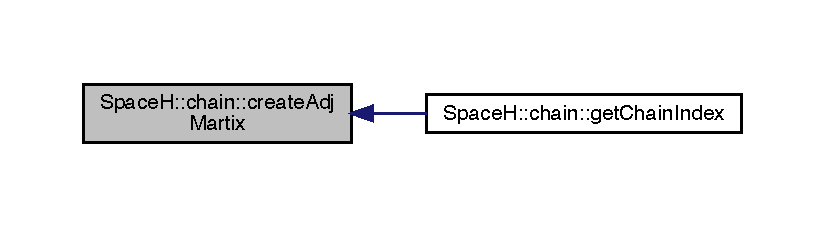
\includegraphics[width=350pt]{namespace_space_h_1_1chain_a8d2f8c8026f24294d16309c4f2e11fdb_icgraph}
\end{center}
\end{figure}
\mbox{\Hypertarget{namespace_space_h_1_1chain_a65d906373401066033d8e4a6ad581cce}\label{namespace_space_h_1_1chain_a65d906373401066033d8e4a6ad581cce}} 
\index{Space\+H\+::chain_@{Space\+H\+::chain_}!create\+Chain\+Index@{create\+Chain\+Index}}
\index{create\+Chain\+Index@{create\+Chain\+Index}!Space\+H\+::chain_@{Space\+H\+::chain_}}
\subsubsection{\texorpdfstring{create\+Chain\+Index()}{createChainIndex()}}
{\footnotesize\ttfamily template$<$typename Node\+Array , typename Index\+Array $>$ \\
void Space\+H\+::chain_\+::create\+Chain\+Index (\begin{DoxyParamCaption}\item[{Node\+Array \&}]{Adj\+Matrix,  }\item[{Index\+Array \&}]{chain_\+Index }\end{DoxyParamCaption})}



Create mapping index from adjoint matrix. 

Create mapping index from sorted elements of adjoint matrix and connect them to a chain_ consequently.
\begin{DoxyParams}{Parameters}
{\em Adj\+Matrix} & The adjoint matrix. \\
\hline
{\em chain_\+Index} & The maping index needs to be calculated as a return value. \\
\hline
\end{DoxyParams}
Here is the caller graph for this function\+:\nopagebreak
\begin{figure}[H]
\begin{center}
\leavevmode
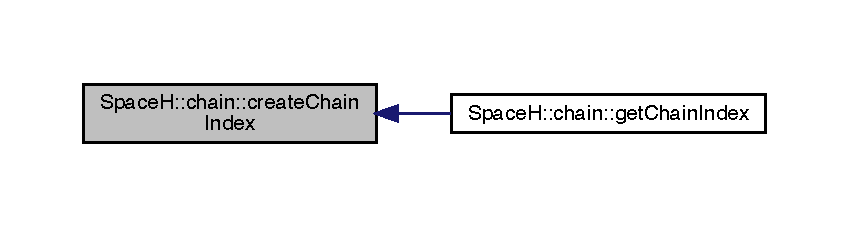
\includegraphics[width=350pt]{namespace_space_h_1_1chain_a65d906373401066033d8e4a6ad581cce_icgraph}
\end{center}
\end{figure}
\mbox{\Hypertarget{namespace_space_h_1_1chain_a9f1ed51f097bc8cf691a87b97639dde9}\label{namespace_space_h_1_1chain_a9f1ed51f097bc8cf691a87b97639dde9}} 
\index{Space\+H\+::chain_@{Space\+H\+::chain_}!get\+Chain\+Index@{get\+Chain\+Index}}
\index{get\+Chain\+Index@{get\+Chain\+Index}!Space\+H\+::chain_@{Space\+H\+::chain_}}
\subsubsection{\texorpdfstring{get\+Chain\+Index()}{getChainIndex()}}
{\footnotesize\ttfamily template$<$typename Vector\+Array , typename Index\+Array $>$ \\
void Space\+H\+::chain_\+::get\+Chain\+Index (\begin{DoxyParamCaption}\item[{const Vector\+Array \&}]{pos,  }\item[{Index\+Array \&}]{chain_\+Index }\end{DoxyParamCaption})}



Calculate the mapping index from Cartesian coordinate to chain_ coordinate.

Find the mapping index from Cartesian coordinate to chain_ coordinate. The chain_ is formed by connecting the nearest particle pairs consequently.
\begin{DoxyParams}{Parameters}
{\em pos} & The array of particle position, used to calculate the distance of particle pairs. \\
\hline
{\em chain_\+Index} & The maping index needs to be calculated as a return value. \\
\hline
\end{DoxyParams}
Here is the call graph for this function\+:\nopagebreak
\begin{figure}[H]
\begin{center}
\leavevmode
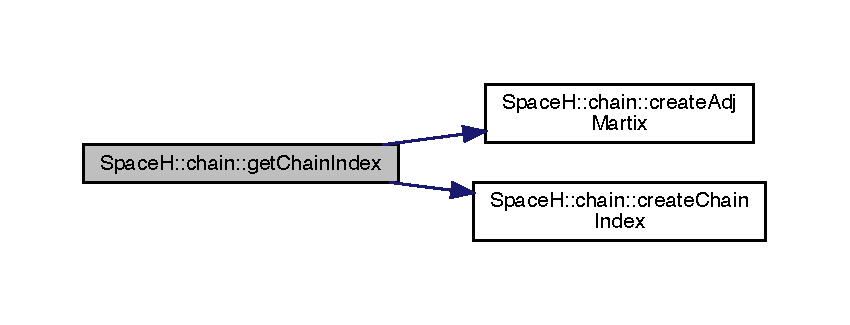
\includegraphics[width=350pt]{namespace_space_h_1_1chain_a9f1ed51f097bc8cf691a87b97639dde9_cgraph}
\end{center}
\end{figure}
Here is the caller graph for this function\+:
\nopagebreak
\begin{figure}[H]
\begin{center}
\leavevmode
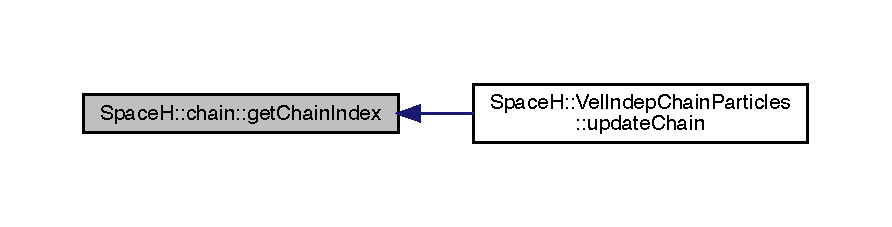
\includegraphics[width=350pt]{namespace_space_h_1_1chain_a9f1ed51f097bc8cf691a87b97639dde9_icgraph}
\end{center}
\end{figure}
\mbox{\Hypertarget{namespace_space_h_1_1chain_ab54ce920a542c01625ee7d6c625cc5c4}\label{namespace_space_h_1_1chain_ab54ce920a542c01625ee7d6c625cc5c4}} 
\index{Space\+H\+::chain_@{Space\+H\+::chain_}!is\+Diff@{is\+Diff}}
\index{is\+Diff@{is\+Diff}!Space\+H\+::chain_@{Space\+H\+::chain_}}
\subsubsection{\texorpdfstring{is\+Diff()}{isDiff()}}
{\footnotesize\ttfamily template$<$typename Index\+Array $>$ \\
bool Space\+H\+::chain_\+::is\+Diff (\begin{DoxyParamCaption}\item[{const Index\+Array \&}]{Index1,  }\item[{const Index\+Array \&}]{Index2 }\end{DoxyParamCaption})}



Check if two mapping indexes are the same. 

Checking the identity of two chain_ index mappings.
\begin{DoxyParams}{Parameters}
{\em Index1} & The first index array. \\
\hline
{\em Index2} & The second index array. \\
\hline
\end{DoxyParams}
\begin{DoxyReturn}{Returns}
boolean 
\end{DoxyReturn}
\begin{DoxyNote}{Note}
\mbox{[}2,4,5,3,1\mbox{]} is identical to \mbox{[}1,3,5,4,2\mbox{]} 
\end{DoxyNote}
Here is the caller graph for this function\+:
\nopagebreak
\begin{figure}[H]
\begin{center}
\leavevmode
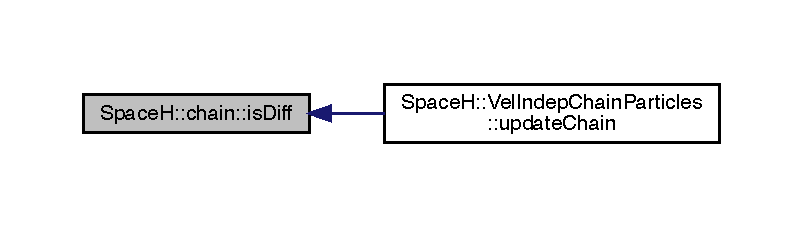
\includegraphics[width=350pt]{namespace_space_h_1_1chain_ab54ce920a542c01625ee7d6c625cc5c4_icgraph}
\end{center}
\end{figure}
\mbox{\Hypertarget{namespace_space_h_1_1chain_a1ba7809b40a52959d0566753b1c2eaee}\label{namespace_space_h_1_1chain_a1ba7809b40a52959d0566753b1c2eaee}} 
\index{Space\+H\+::chain_@{Space\+H\+::chain_}!syn\+Cartesian@{syn\+Cartesian}}
\index{syn\+Cartesian@{syn\+Cartesian}!Space\+H\+::chain_@{Space\+H\+::chain_}}
\subsubsection{\texorpdfstring{syn\+Cartesian()}{synCartesian()}}
{\footnotesize\ttfamily template$<$typename Vector\+Array , typename Index\+Array $>$ \\
void Space\+H\+::chain_\+::syn\+Cartesian (\begin{DoxyParamCaption}\item[{const Vector\+Array \&}]{chain_\+Data,  }\item[{Vector\+Array \&}]{data,  }\item[{const Index\+Array \&}]{chain_\+Index }\end{DoxyParamCaption})}



Calulate the Cartesian data from chain_ data and chain_ index mapping.


\begin{DoxyParams}{Parameters}
{\em chain_\+Data} & Data in chain_ coordinates. \\
\hline
{\em data} & Data need to be calculated in Cartesian coordinates. \\
\hline
{\em chain_\+Index} & Chain index mapping. \\
\hline
\end{DoxyParams}
\begin{DoxyNote}{Note}
This function should be a inverse transformation of \mbox{\hyperlink{namespace_space_h_1_1chain_a218de9c738267dd3efceebfda0a90a43}{syn\+Chain()}}. 
\end{DoxyNote}
Here is the caller graph for this function\+:
\nopagebreak
\begin{figure}[H]
\begin{center}
\leavevmode
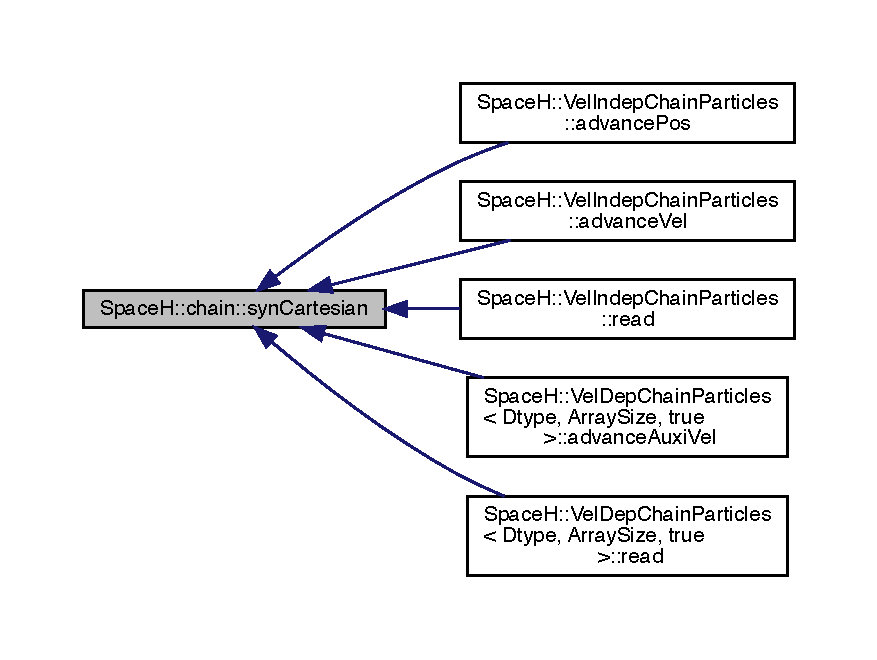
\includegraphics[width=350pt]{namespace_space_h_1_1chain_a1ba7809b40a52959d0566753b1c2eaee_icgraph}
\end{center}
\end{figure}
\mbox{\Hypertarget{namespace_space_h_1_1chain_a218de9c738267dd3efceebfda0a90a43}\label{namespace_space_h_1_1chain_a218de9c738267dd3efceebfda0a90a43}} 
\index{Space\+H\+::chain_@{Space\+H\+::chain_}!syn\+Chain@{syn\+Chain}}
\index{syn\+Chain@{syn\+Chain}!Space\+H\+::chain_@{Space\+H\+::chain_}}
\subsubsection{\texorpdfstring{syn\+Chain()}{synChain()}}
{\footnotesize\ttfamily template$<$typename Vector\+Array , typename Index\+Array $>$ \\
void Space\+H\+::chain_\+::syn\+Chain (\begin{DoxyParamCaption}\item[{const Vector\+Array \&}]{data,  }\item[{Vector\+Array \&}]{chain_\+Data,  }\item[{const Index\+Array \&}]{chain_\+Index }\end{DoxyParamCaption})}



Calulate the chain_ data from Cartesian data and chain_ index mapping.


\begin{DoxyParams}{Parameters}
{\em data} & Data in Cartesian coordinates. \\
\hline
{\em chain_\+Data} & Data need to be calculated in chain_ coordinates. \\
\hline
{\em chain_\+Index} & Chain index mapping. \\
\hline
\end{DoxyParams}
\begin{DoxyNote}{Note}
This function should be a inverse transformation of \mbox{\hyperlink{namespace_space_h_1_1chain_a1ba7809b40a52959d0566753b1c2eaee}{syn\+Cartesian()}}. 
\end{DoxyNote}
Here is the caller graph for this function\+:
\nopagebreak
\begin{figure}[H]
\begin{center}
\leavevmode
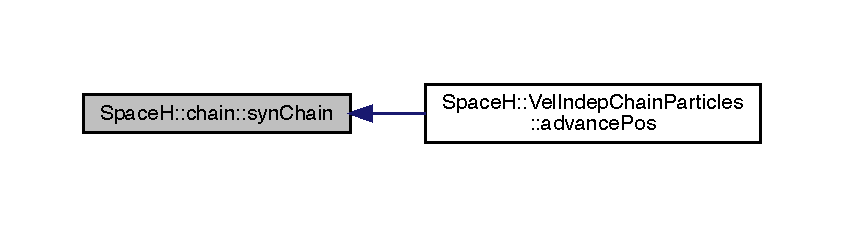
\includegraphics[width=350pt]{namespace_space_h_1_1chain_a218de9c738267dd3efceebfda0a90a43_icgraph}
\end{center}
\end{figure}
\mbox{\Hypertarget{namespace_space_h_1_1chain_a631ad6a37f246a0db64e5879825a6878}\label{namespace_space_h_1_1chain_a631ad6a37f246a0db64e5879825a6878}} 
\index{Space\+H\+::chain_@{Space\+H\+::chain_}!update\+Chain@{update\+Chain}}
\index{update\+Chain@{update\+Chain}!Space\+H\+::chain_@{Space\+H\+::chain_}}
\subsubsection{\texorpdfstring{update\+Chain()}{updateChain()}}
{\footnotesize\ttfamily template$<$typename Vector\+Array , typename Index\+Array $>$ \\
void Space\+H\+::chain_\+::update\+Chain (\begin{DoxyParamCaption}\item[{Vector\+Array \&}]{pos,  }\item[{Index\+Array \&}]{chain_\+Index,  }\item[{Index\+Array \&}]{new\+Index }\end{DoxyParamCaption})}



Update the position chain_.

Update the position chain_. Due to the evolution, the chain_ index mapping could change with time, this function is used to update the position chain_ with old chain_ data.
\begin{DoxyParams}{Parameters}
{\em pos} & The old chain_ position array needs update. \\
\hline
{\em chain_\+Index} & The old chain_ index mapping. \\
\hline
{\em new\+Index} & The new chain_ index mapping. \\
\hline
\end{DoxyParams}
Here is the caller graph for this function\+:
\nopagebreak
\begin{figure}[H]
\begin{center}
\leavevmode
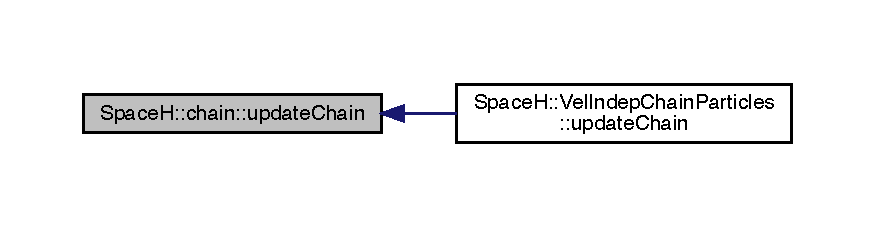
\includegraphics[width=350pt]{namespace_space_h_1_1chain_a631ad6a37f246a0db64e5879825a6878_icgraph}
\end{center}
\end{figure}

\hypertarget{namespace_space_h_1_1_const}{}\section{SpaceH\+:\+:Const Namespace Reference}
\label{namespace_space_h_1_1_const}\index{Space\+H\+::\+Const@{Space\+H\+::\+Const}}
\subsection*{Variables}
\begin{DoxyCompactItemize}
\item 
constexpr double \mbox{\hyperlink{namespace_space_h_1_1_const_a453eccad0d73caeedd6168a50d04d190}{I\+N\+V\+\_\+C}} = 1 / \mbox{\hyperlink{namespace_space_h_1_1_const_a2d7bff2e7b11ffe2fcc07333089c83a4}{C}}
\item 
constexpr double \mbox{\hyperlink{namespace_space_h_1_1_const_ac438c0ca124c73e6a55ef0d4afd05551}{I\+N\+V\+\_\+\+C2}} = \mbox{\hyperlink{namespace_space_h_1_1_const_a453eccad0d73caeedd6168a50d04d190}{I\+N\+V\+\_\+C}} $\ast$ \mbox{\hyperlink{namespace_space_h_1_1_const_a453eccad0d73caeedd6168a50d04d190}{I\+N\+V\+\_\+C}}
\item 
constexpr double \mbox{\hyperlink{namespace_space_h_1_1_const_a8a27f7c32317db823a656ceeaf6223dd}{I\+N\+V\+\_\+\+C3}} = \mbox{\hyperlink{namespace_space_h_1_1_const_ac438c0ca124c73e6a55ef0d4afd05551}{I\+N\+V\+\_\+\+C2}} $\ast$ \mbox{\hyperlink{namespace_space_h_1_1_const_a453eccad0d73caeedd6168a50d04d190}{I\+N\+V\+\_\+C}}
\item 
constexpr double \mbox{\hyperlink{namespace_space_h_1_1_const_a2adde6a8a2a2def2a09e650f6cdcbf98}{I\+N\+V\+\_\+\+C4}} = \mbox{\hyperlink{namespace_space_h_1_1_const_a8a27f7c32317db823a656ceeaf6223dd}{I\+N\+V\+\_\+\+C3}} $\ast$ \mbox{\hyperlink{namespace_space_h_1_1_const_a453eccad0d73caeedd6168a50d04d190}{I\+N\+V\+\_\+C}}
\item 
constexpr double \mbox{\hyperlink{namespace_space_h_1_1_const_a6e9515f852a58219dbb6ceb0f8b381a2}{I\+N\+V\+\_\+\+C5}} = \mbox{\hyperlink{namespace_space_h_1_1_const_a2adde6a8a2a2def2a09e650f6cdcbf98}{I\+N\+V\+\_\+\+C4}} $\ast$ \mbox{\hyperlink{namespace_space_h_1_1_const_a453eccad0d73caeedd6168a50d04d190}{I\+N\+V\+\_\+C}}
\item 
constexpr double \mbox{\hyperlink{namespace_space_h_1_1_const_afdcc70c6f78ec4cf7baad3525ba7c618}{PI}} = 3.\+14159265358979323
\item 
constexpr double \mbox{\hyperlink{namespace_space_h_1_1_const_ac17bec90d7d2b75f8f056347c7d6ced6}{G}} = 1
\item 
constexpr double \mbox{\hyperlink{namespace_space_h_1_1_const_a2d7bff2e7b11ffe2fcc07333089c83a4}{C}} = 299792.\+458 $\ast$ \mbox{\hyperlink{namespace_space_h_1_1_unit_a94c0a976eb50dcc88f04f3513049e8c3}{Unit\+::\+K\+MS}}
\end{DoxyCompactItemize}


\subsection{Variable Documentation}
\mbox{\Hypertarget{namespace_space_h_1_1_const_a2d7bff2e7b11ffe2fcc07333089c83a4}\label{namespace_space_h_1_1_const_a2d7bff2e7b11ffe2fcc07333089c83a4}} 
\index{Space\+H\+::\+Const@{Space\+H\+::\+Const}!C@{C}}
\index{C@{C}!Space\+H\+::\+Const@{Space\+H\+::\+Const}}
\subsubsection{\texorpdfstring{C}{C}}
{\footnotesize\ttfamily constexpr double Space\+H\+::\+Const\+::C = 299792.\+458 $\ast$ \mbox{\hyperlink{namespace_space_h_1_1_unit_a94c0a976eb50dcc88f04f3513049e8c3}{Unit\+::\+K\+MS}}}

\mbox{\Hypertarget{namespace_space_h_1_1_const_ac17bec90d7d2b75f8f056347c7d6ced6}\label{namespace_space_h_1_1_const_ac17bec90d7d2b75f8f056347c7d6ced6}} 
\index{Space\+H\+::\+Const@{Space\+H\+::\+Const}!G@{G}}
\index{G@{G}!Space\+H\+::\+Const@{Space\+H\+::\+Const}}
\subsubsection{\texorpdfstring{G}{G}}
{\footnotesize\ttfamily constexpr double Space\+H\+::\+Const\+::G = 1}

\mbox{\Hypertarget{namespace_space_h_1_1_const_a453eccad0d73caeedd6168a50d04d190}\label{namespace_space_h_1_1_const_a453eccad0d73caeedd6168a50d04d190}} 
\index{Space\+H\+::\+Const@{Space\+H\+::\+Const}!I\+N\+V\+\_\+C@{I\+N\+V\+\_\+C}}
\index{I\+N\+V\+\_\+C@{I\+N\+V\+\_\+C}!Space\+H\+::\+Const@{Space\+H\+::\+Const}}
\subsubsection{\texorpdfstring{I\+N\+V\+\_\+C}{INV\_C}}
{\footnotesize\ttfamily constexpr double Space\+H\+::\+Const\+::\+I\+N\+V\+\_\+C = 1 / \mbox{\hyperlink{namespace_space_h_1_1_const_a2d7bff2e7b11ffe2fcc07333089c83a4}{C}}}

\mbox{\Hypertarget{namespace_space_h_1_1_const_ac438c0ca124c73e6a55ef0d4afd05551}\label{namespace_space_h_1_1_const_ac438c0ca124c73e6a55ef0d4afd05551}} 
\index{Space\+H\+::\+Const@{Space\+H\+::\+Const}!I\+N\+V\+\_\+\+C2@{I\+N\+V\+\_\+\+C2}}
\index{I\+N\+V\+\_\+\+C2@{I\+N\+V\+\_\+\+C2}!Space\+H\+::\+Const@{Space\+H\+::\+Const}}
\subsubsection{\texorpdfstring{I\+N\+V\+\_\+\+C2}{INV\_C2}}
{\footnotesize\ttfamily constexpr double Space\+H\+::\+Const\+::\+I\+N\+V\+\_\+\+C2 = \mbox{\hyperlink{namespace_space_h_1_1_const_a453eccad0d73caeedd6168a50d04d190}{I\+N\+V\+\_\+C}} $\ast$ \mbox{\hyperlink{namespace_space_h_1_1_const_a453eccad0d73caeedd6168a50d04d190}{I\+N\+V\+\_\+C}}}

\mbox{\Hypertarget{namespace_space_h_1_1_const_a8a27f7c32317db823a656ceeaf6223dd}\label{namespace_space_h_1_1_const_a8a27f7c32317db823a656ceeaf6223dd}} 
\index{Space\+H\+::\+Const@{Space\+H\+::\+Const}!I\+N\+V\+\_\+\+C3@{I\+N\+V\+\_\+\+C3}}
\index{I\+N\+V\+\_\+\+C3@{I\+N\+V\+\_\+\+C3}!Space\+H\+::\+Const@{Space\+H\+::\+Const}}
\subsubsection{\texorpdfstring{I\+N\+V\+\_\+\+C3}{INV\_C3}}
{\footnotesize\ttfamily constexpr double Space\+H\+::\+Const\+::\+I\+N\+V\+\_\+\+C3 = \mbox{\hyperlink{namespace_space_h_1_1_const_ac438c0ca124c73e6a55ef0d4afd05551}{I\+N\+V\+\_\+\+C2}} $\ast$ \mbox{\hyperlink{namespace_space_h_1_1_const_a453eccad0d73caeedd6168a50d04d190}{I\+N\+V\+\_\+C}}}

\mbox{\Hypertarget{namespace_space_h_1_1_const_a2adde6a8a2a2def2a09e650f6cdcbf98}\label{namespace_space_h_1_1_const_a2adde6a8a2a2def2a09e650f6cdcbf98}} 
\index{Space\+H\+::\+Const@{Space\+H\+::\+Const}!I\+N\+V\+\_\+\+C4@{I\+N\+V\+\_\+\+C4}}
\index{I\+N\+V\+\_\+\+C4@{I\+N\+V\+\_\+\+C4}!Space\+H\+::\+Const@{Space\+H\+::\+Const}}
\subsubsection{\texorpdfstring{I\+N\+V\+\_\+\+C4}{INV\_C4}}
{\footnotesize\ttfamily constexpr double Space\+H\+::\+Const\+::\+I\+N\+V\+\_\+\+C4 = \mbox{\hyperlink{namespace_space_h_1_1_const_a8a27f7c32317db823a656ceeaf6223dd}{I\+N\+V\+\_\+\+C3}} $\ast$ \mbox{\hyperlink{namespace_space_h_1_1_const_a453eccad0d73caeedd6168a50d04d190}{I\+N\+V\+\_\+C}}}

\mbox{\Hypertarget{namespace_space_h_1_1_const_a6e9515f852a58219dbb6ceb0f8b381a2}\label{namespace_space_h_1_1_const_a6e9515f852a58219dbb6ceb0f8b381a2}} 
\index{Space\+H\+::\+Const@{Space\+H\+::\+Const}!I\+N\+V\+\_\+\+C5@{I\+N\+V\+\_\+\+C5}}
\index{I\+N\+V\+\_\+\+C5@{I\+N\+V\+\_\+\+C5}!Space\+H\+::\+Const@{Space\+H\+::\+Const}}
\subsubsection{\texorpdfstring{I\+N\+V\+\_\+\+C5}{INV\_C5}}
{\footnotesize\ttfamily constexpr double Space\+H\+::\+Const\+::\+I\+N\+V\+\_\+\+C5 = \mbox{\hyperlink{namespace_space_h_1_1_const_a2adde6a8a2a2def2a09e650f6cdcbf98}{I\+N\+V\+\_\+\+C4}} $\ast$ \mbox{\hyperlink{namespace_space_h_1_1_const_a453eccad0d73caeedd6168a50d04d190}{I\+N\+V\+\_\+C}}}

\mbox{\Hypertarget{namespace_space_h_1_1_const_afdcc70c6f78ec4cf7baad3525ba7c618}\label{namespace_space_h_1_1_const_afdcc70c6f78ec4cf7baad3525ba7c618}} 
\index{Space\+H\+::\+Const@{Space\+H\+::\+Const}!PI@{PI}}
\index{PI@{PI}!Space\+H\+::\+Const@{Space\+H\+::\+Const}}
\subsubsection{\texorpdfstring{PI}{PI}}
{\footnotesize\ttfamily constexpr double Space\+H\+::\+Const\+::\+PI = 3.\+14159265358979323}


\hypertarget{namespace_space_h_1_1_oc_tree}{}\section{SpaceH\+:\+:Oc\+Tree Namespace Reference}
\label{namespace_space_h_1_1_oc_tree}\index{Space\+H\+::\+Oc\+Tree@{Space\+H\+::\+Oc\+Tree}}
\subsection*{Classes}
\begin{DoxyCompactItemize}
\item 
struct \mbox{\hyperlink{struct_space_h_1_1_oc_tree_1_1_coord}{Coord}}
\item 
struct \mbox{\hyperlink{struct_space_h_1_1_oc_tree_1_1empty_parent_node}{empty\+Parent\+Node}}
\item 
struct \mbox{\hyperlink{struct_space_h_1_1_oc_tree_1_1_list}{List}}
\item 
struct \mbox{\hyperlink{struct_space_h_1_1_oc_tree_1_1_list_node}{List\+Node}}
\item 
struct \mbox{\hyperlink{struct_space_h_1_1_oc_tree_1_1_oct}{Oct}}
\item 
struct \mbox{\hyperlink{struct_space_h_1_1_oc_tree_1_1_octree}{Octree}}
\item 
struct \mbox{\hyperlink{struct_space_h_1_1_oc_tree_1_1_octree_node}{Octree\+Node}}
\end{DoxyCompactItemize}
\subsection*{Functions}
\begin{DoxyCompactItemize}
\item 
{\footnotesize template$<$typename List , typename T $>$ }\\void \mbox{\hyperlink{namespace_space_h_1_1_oc_tree_af27f1253cb5f80c85149b2ccbc2b6f0b}{split\+Oct}} (\mbox{\hyperlink{struct_space_h_1_1_oc_tree_1_1_list}{List}} \&raw\+List, \mbox{\hyperlink{struct_space_h_1_1_oc_tree_1_1_oct}{Oct}}$<$ \mbox{\hyperlink{struct_space_h_1_1_oc_tree_1_1_list}{List}} $>$ \&Lists, T xmid, T ymid, T zmid)
\end{DoxyCompactItemize}


\subsection{Function Documentation}
\mbox{\Hypertarget{namespace_space_h_1_1_oc_tree_af27f1253cb5f80c85149b2ccbc2b6f0b}\label{namespace_space_h_1_1_oc_tree_af27f1253cb5f80c85149b2ccbc2b6f0b}} 
\index{Space\+H\+::\+Oc\+Tree@{Space\+H\+::\+Oc\+Tree}!split\+Oct@{split\+Oct}}
\index{split\+Oct@{split\+Oct}!Space\+H\+::\+Oc\+Tree@{Space\+H\+::\+Oc\+Tree}}
\subsubsection{\texorpdfstring{split\+Oct()}{splitOct()}}
{\footnotesize\ttfamily template$<$typename List , typename T $>$ \\
void Space\+H\+::\+Oc\+Tree\+::split\+Oct (\begin{DoxyParamCaption}\item[{\mbox{\hyperlink{struct_space_h_1_1_oc_tree_1_1_list}{List}} \&}]{raw\+List,  }\item[{\mbox{\hyperlink{struct_space_h_1_1_oc_tree_1_1_oct}{Oct}}$<$ \mbox{\hyperlink{struct_space_h_1_1_oc_tree_1_1_list}{List}} $>$ \&}]{Lists,  }\item[{T}]{xmid,  }\item[{T}]{ymid,  }\item[{T}]{zmid }\end{DoxyParamCaption})}

Here is the call graph for this function\+:
\nopagebreak
\begin{figure}[H]
\begin{center}
\leavevmode
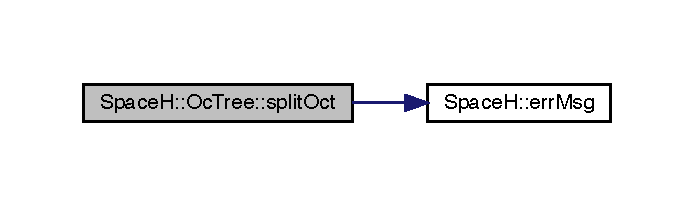
\includegraphics[width=333pt]{namespace_space_h_1_1_oc_tree_af27f1253cb5f80c85149b2ccbc2b6f0b_cgraph}
\end{center}
\end{figure}

\hypertarget{namespace_space_h_1_1_orbits}{}\section{SpaceH\+:\+:Orbits Namespace Reference}
\label{namespace_space_h_1_1_orbits}\index{Space\+H\+::\+Orbits@{Space\+H\+::\+Orbits}}
\subsection*{Classes}
\begin{DoxyCompactItemize}
\item 
struct \mbox{\hyperlink{struct_space_h_1_1_orbits_1_1_param}{Param}}
\end{DoxyCompactItemize}
\subsection*{Functions}
\begin{DoxyCompactItemize}
\item 
{\footnotesize template$<$typename Scalar $>$ }\\\mbox{\hyperlink{create_kepler_8cpp_a8c2981f3f834be9448a6ab06c28748eb}{Scalar}} \mbox{\hyperlink{namespace_space_h_1_1_orbits_a678a54bbf3a8637d6437b4b8b4a39d97}{myacos}} (\mbox{\hyperlink{create_kepler_8cpp_a8c2981f3f834be9448a6ab06c28748eb}{Scalar}} x)
\item 
{\footnotesize template$<$typename Vector , typename Scalar $>$ }\\Vector \mbox{\hyperlink{namespace_space_h_1_1_orbits_a67c6c20142cd8a4bd9690741c61314da}{calcu\+Eccentricity}} (\mbox{\hyperlink{create_kepler_8cpp_a8c2981f3f834be9448a6ab06c28748eb}{Scalar}} m1, \mbox{\hyperlink{create_kepler_8cpp_a8c2981f3f834be9448a6ab06c28748eb}{Scalar}} m2, const Vector \&pos1, const Vector \&pos2, const Vector \&vel1, const Vector \&vel2)
\item 
{\footnotesize template$<$typename Vector , typename Scalar $>$ }\\\mbox{\hyperlink{create_kepler_8cpp_a8c2981f3f834be9448a6ab06c28748eb}{Scalar}} \mbox{\hyperlink{namespace_space_h_1_1_orbits_ad5dd14dac8365a426bc0ff7452318835}{calcu\+Semi\+Major\+Axis}} (\mbox{\hyperlink{create_kepler_8cpp_a8c2981f3f834be9448a6ab06c28748eb}{Scalar}} m1, \mbox{\hyperlink{create_kepler_8cpp_a8c2981f3f834be9448a6ab06c28748eb}{Scalar}} m2, const Vector \&pos1, const Vector \&pos2, const Vector \&vel1, const Vector \&vel2)
\item 
{\footnotesize template$<$typename Vector , typename Scalar $>$ }\\void \mbox{\hyperlink{namespace_space_h_1_1_orbits_a5e8b37a1237e17770907f5c2adbb53d6}{to\+Oribt\+Parameters}} (\mbox{\hyperlink{create_kepler_8cpp_a8c2981f3f834be9448a6ab06c28748eb}{Scalar}} m1, \mbox{\hyperlink{create_kepler_8cpp_a8c2981f3f834be9448a6ab06c28748eb}{Scalar}} m2, const Vector \&pos1, const Vector \&pos2, const Vector \&vel1, const Vector \&vel2, \mbox{\hyperlink{struct_space_h_1_1_orbits_1_1_param}{Param}}$<$ \mbox{\hyperlink{create_kepler_8cpp_a8c2981f3f834be9448a6ab06c28748eb}{Scalar}} $>$ \&params)
\item 
{\footnotesize template$<$typename Vector , typename Scalar $>$ }\\void \mbox{\hyperlink{namespace_space_h_1_1_orbits_ab06b7e85a786928255938378f9a97e26}{euler\+Rotate}} (Vector \&v, const \mbox{\hyperlink{create_kepler_8cpp_a8c2981f3f834be9448a6ab06c28748eb}{Scalar}} phi, const \mbox{\hyperlink{create_kepler_8cpp_a8c2981f3f834be9448a6ab06c28748eb}{Scalar}} theta, const \mbox{\hyperlink{create_kepler_8cpp_a8c2981f3f834be9448a6ab06c28748eb}{Scalar}} psi)
\item 
{\footnotesize template$<$typename Scalar $>$ }\\\mbox{\hyperlink{create_kepler_8cpp_a8c2981f3f834be9448a6ab06c28748eb}{Scalar}} \mbox{\hyperlink{namespace_space_h_1_1_orbits_ab0a6bf4bbce5725fa15cc6250057817c}{get\+Random\+Mean\+Anomaly}} (\mbox{\hyperlink{create_kepler_8cpp_a8c2981f3f834be9448a6ab06c28748eb}{Scalar}} e, \mbox{\hyperlink{create_kepler_8cpp_a8c2981f3f834be9448a6ab06c28748eb}{Scalar}} Mmin, \mbox{\hyperlink{create_kepler_8cpp_a8c2981f3f834be9448a6ab06c28748eb}{Scalar}} Mmax)
\item 
{\footnotesize template$<$typename Scalar $>$ }\\\mbox{\hyperlink{create_kepler_8cpp_a8c2981f3f834be9448a6ab06c28748eb}{Scalar}} \mbox{\hyperlink{namespace_space_h_1_1_orbits_a43d1a07ed25eaf775f3a83d7000a2596}{get\+True\+Anomaly}} (\mbox{\hyperlink{create_kepler_8cpp_a8c2981f3f834be9448a6ab06c28748eb}{Scalar}} E, \mbox{\hyperlink{create_kepler_8cpp_a8c2981f3f834be9448a6ab06c28748eb}{Scalar}} e)
\item 
{\footnotesize template$<$typename Scalar $>$ }\\\mbox{\hyperlink{create_kepler_8cpp_a8c2981f3f834be9448a6ab06c28748eb}{Scalar}} \mbox{\hyperlink{namespace_space_h_1_1_orbits_a729783768420346b170d79aa5e196841}{get\+Eccentric\+Anomaly}} (\mbox{\hyperlink{create_kepler_8cpp_a8c2981f3f834be9448a6ab06c28748eb}{Scalar}} M, \mbox{\hyperlink{create_kepler_8cpp_a8c2981f3f834be9448a6ab06c28748eb}{Scalar}} e)
\end{DoxyCompactItemize}


\subsection{Function Documentation}
\mbox{\Hypertarget{namespace_space_h_1_1_orbits_a67c6c20142cd8a4bd9690741c61314da}\label{namespace_space_h_1_1_orbits_a67c6c20142cd8a4bd9690741c61314da}} 
\index{Space\+H\+::\+Orbits@{Space\+H\+::\+Orbits}!calcu\+Eccentricity@{calcu\+Eccentricity}}
\index{calcu\+Eccentricity@{calcu\+Eccentricity}!Space\+H\+::\+Orbits@{Space\+H\+::\+Orbits}}
\subsubsection{\texorpdfstring{calcu\+Eccentricity()}{calcuEccentricity()}}
{\footnotesize\ttfamily template$<$typename Vector , typename Scalar $>$ \\
Vector Space\+H\+::\+Orbits\+::calcu\+Eccentricity (\begin{DoxyParamCaption}\item[{\mbox{\hyperlink{create_kepler_8cpp_a8c2981f3f834be9448a6ab06c28748eb}{Scalar}}}]{m1,  }\item[{\mbox{\hyperlink{create_kepler_8cpp_a8c2981f3f834be9448a6ab06c28748eb}{Scalar}}}]{m2,  }\item[{const Vector \&}]{pos1,  }\item[{const Vector \&}]{pos2,  }\item[{const Vector \&}]{vel1,  }\item[{const Vector \&}]{vel2 }\end{DoxyParamCaption})\hspace{0.3cm}{\ttfamily [inline]}}

Here is the call graph for this function\+:
\nopagebreak
\begin{figure}[H]
\begin{center}
\leavevmode
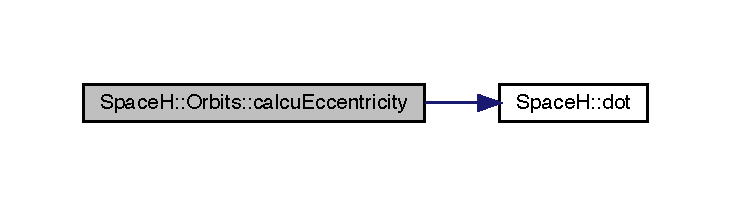
\includegraphics[width=350pt]{namespace_space_h_1_1_orbits_a67c6c20142cd8a4bd9690741c61314da_cgraph}
\end{center}
\end{figure}
\mbox{\Hypertarget{namespace_space_h_1_1_orbits_ad5dd14dac8365a426bc0ff7452318835}\label{namespace_space_h_1_1_orbits_ad5dd14dac8365a426bc0ff7452318835}} 
\index{Space\+H\+::\+Orbits@{Space\+H\+::\+Orbits}!calcu\+Semi\+Major\+Axis@{calcu\+Semi\+Major\+Axis}}
\index{calcu\+Semi\+Major\+Axis@{calcu\+Semi\+Major\+Axis}!Space\+H\+::\+Orbits@{Space\+H\+::\+Orbits}}
\subsubsection{\texorpdfstring{calcu\+Semi\+Major\+Axis()}{calcuSemiMajorAxis()}}
{\footnotesize\ttfamily template$<$typename Vector , typename Scalar $>$ \\
\mbox{\hyperlink{create_kepler_8cpp_a8c2981f3f834be9448a6ab06c28748eb}{Scalar}} Space\+H\+::\+Orbits\+::calcu\+Semi\+Major\+Axis (\begin{DoxyParamCaption}\item[{\mbox{\hyperlink{create_kepler_8cpp_a8c2981f3f834be9448a6ab06c28748eb}{Scalar}}}]{m1,  }\item[{\mbox{\hyperlink{create_kepler_8cpp_a8c2981f3f834be9448a6ab06c28748eb}{Scalar}}}]{m2,  }\item[{const Vector \&}]{pos1,  }\item[{const Vector \&}]{pos2,  }\item[{const Vector \&}]{vel1,  }\item[{const Vector \&}]{vel2 }\end{DoxyParamCaption})\hspace{0.3cm}{\ttfamily [inline]}}

\mbox{\Hypertarget{namespace_space_h_1_1_orbits_ab06b7e85a786928255938378f9a97e26}\label{namespace_space_h_1_1_orbits_ab06b7e85a786928255938378f9a97e26}} 
\index{Space\+H\+::\+Orbits@{Space\+H\+::\+Orbits}!euler\+Rotate@{euler\+Rotate}}
\index{euler\+Rotate@{euler\+Rotate}!Space\+H\+::\+Orbits@{Space\+H\+::\+Orbits}}
\subsubsection{\texorpdfstring{euler\+Rotate()}{eulerRotate()}}
{\footnotesize\ttfamily template$<$typename Vector , typename Scalar $>$ \\
void Space\+H\+::\+Orbits\+::euler\+Rotate (\begin{DoxyParamCaption}\item[{Vector \&}]{v,  }\item[{const \mbox{\hyperlink{create_kepler_8cpp_a8c2981f3f834be9448a6ab06c28748eb}{Scalar}}}]{phi,  }\item[{const \mbox{\hyperlink{create_kepler_8cpp_a8c2981f3f834be9448a6ab06c28748eb}{Scalar}}}]{theta,  }\item[{const \mbox{\hyperlink{create_kepler_8cpp_a8c2981f3f834be9448a6ab06c28748eb}{Scalar}}}]{psi }\end{DoxyParamCaption})}

\mbox{\Hypertarget{namespace_space_h_1_1_orbits_a729783768420346b170d79aa5e196841}\label{namespace_space_h_1_1_orbits_a729783768420346b170d79aa5e196841}} 
\index{Space\+H\+::\+Orbits@{Space\+H\+::\+Orbits}!get\+Eccentric\+Anomaly@{get\+Eccentric\+Anomaly}}
\index{get\+Eccentric\+Anomaly@{get\+Eccentric\+Anomaly}!Space\+H\+::\+Orbits@{Space\+H\+::\+Orbits}}
\subsubsection{\texorpdfstring{get\+Eccentric\+Anomaly()}{calcuEccentricAnomaly()}}
{\footnotesize\ttfamily template$<$typename Scalar $>$ \\
\mbox{\hyperlink{create_kepler_8cpp_a8c2981f3f834be9448a6ab06c28748eb}{Scalar}} Space\+H\+::\+Orbits\+::get\+Eccentric\+Anomaly (\begin{DoxyParamCaption}\item[{\mbox{\hyperlink{create_kepler_8cpp_a8c2981f3f834be9448a6ab06c28748eb}{Scalar}}}]{M,  }\item[{\mbox{\hyperlink{create_kepler_8cpp_a8c2981f3f834be9448a6ab06c28748eb}{Scalar}}}]{e }\end{DoxyParamCaption})}

Here is the call graph for this function\+:
\nopagebreak
\begin{figure}[H]
\begin{center}
\leavevmode
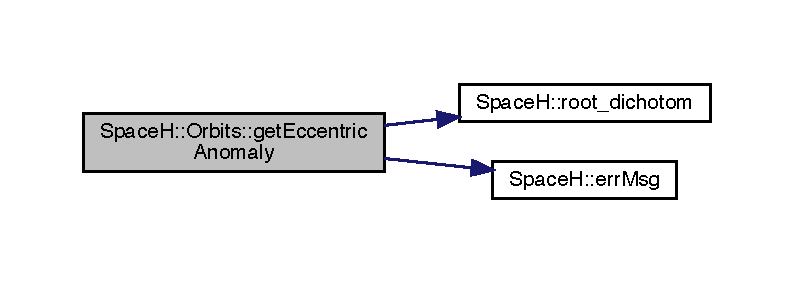
\includegraphics[width=350pt]{namespace_space_h_1_1_orbits_a729783768420346b170d79aa5e196841_cgraph}
\end{center}
\end{figure}
Here is the caller graph for this function\+:
\nopagebreak
\begin{figure}[H]
\begin{center}
\leavevmode
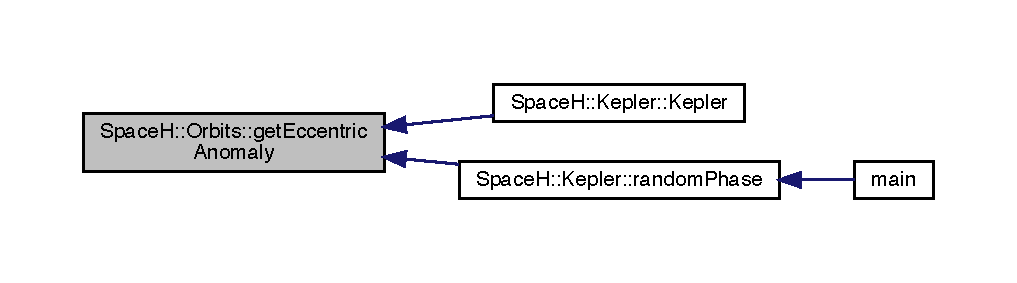
\includegraphics[width=350pt]{namespace_space_h_1_1_orbits_a729783768420346b170d79aa5e196841_icgraph}
\end{center}
\end{figure}
\mbox{\Hypertarget{namespace_space_h_1_1_orbits_ab0a6bf4bbce5725fa15cc6250057817c}\label{namespace_space_h_1_1_orbits_ab0a6bf4bbce5725fa15cc6250057817c}} 
\index{Space\+H\+::\+Orbits@{Space\+H\+::\+Orbits}!get\+Random\+Mean\+Anomaly@{get\+Random\+Mean\+Anomaly}}
\index{get\+Random\+Mean\+Anomaly@{get\+Random\+Mean\+Anomaly}!Space\+H\+::\+Orbits@{Space\+H\+::\+Orbits}}
\subsubsection{\texorpdfstring{get\+Random\+Mean\+Anomaly()}{getRandomMeanAnomaly()}}
{\footnotesize\ttfamily template$<$typename Scalar $>$ \\
\mbox{\hyperlink{create_kepler_8cpp_a8c2981f3f834be9448a6ab06c28748eb}{Scalar}} Space\+H\+::\+Orbits\+::get\+Random\+Mean\+Anomaly (\begin{DoxyParamCaption}\item[{\mbox{\hyperlink{create_kepler_8cpp_a8c2981f3f834be9448a6ab06c28748eb}{Scalar}}}]{e,  }\item[{\mbox{\hyperlink{create_kepler_8cpp_a8c2981f3f834be9448a6ab06c28748eb}{Scalar}}}]{Mmin,  }\item[{\mbox{\hyperlink{create_kepler_8cpp_a8c2981f3f834be9448a6ab06c28748eb}{Scalar}}}]{Mmax }\end{DoxyParamCaption})}

Here is the call graph for this function\+:
\nopagebreak
\begin{figure}[H]
\begin{center}
\leavevmode
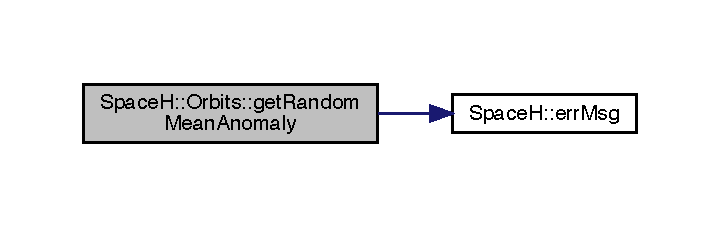
\includegraphics[width=345pt]{namespace_space_h_1_1_orbits_ab0a6bf4bbce5725fa15cc6250057817c_cgraph}
\end{center}
\end{figure}
Here is the caller graph for this function\+:
\nopagebreak
\begin{figure}[H]
\begin{center}
\leavevmode
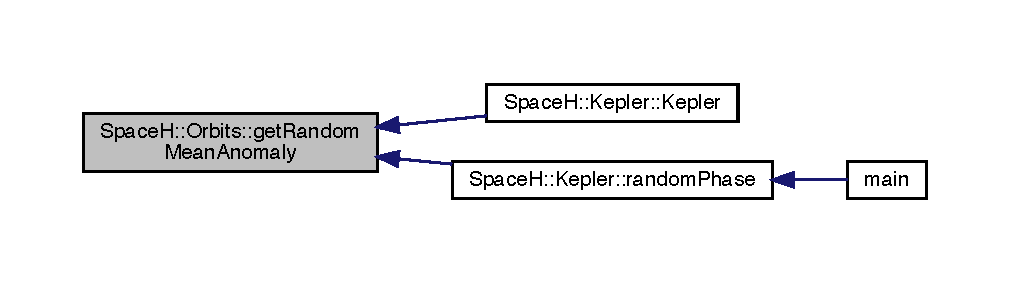
\includegraphics[width=350pt]{namespace_space_h_1_1_orbits_ab0a6bf4bbce5725fa15cc6250057817c_icgraph}
\end{center}
\end{figure}
\mbox{\Hypertarget{namespace_space_h_1_1_orbits_a43d1a07ed25eaf775f3a83d7000a2596}\label{namespace_space_h_1_1_orbits_a43d1a07ed25eaf775f3a83d7000a2596}} 
\index{Space\+H\+::\+Orbits@{Space\+H\+::\+Orbits}!get\+True\+Anomaly@{get\+True\+Anomaly}}
\index{get\+True\+Anomaly@{get\+True\+Anomaly}!Space\+H\+::\+Orbits@{Space\+H\+::\+Orbits}}
\subsubsection{\texorpdfstring{get\+True\+Anomaly()}{calcuTrueAnomaly()}}
{\footnotesize\ttfamily template$<$typename Scalar $>$ \\
\mbox{\hyperlink{create_kepler_8cpp_a8c2981f3f834be9448a6ab06c28748eb}{Scalar}} Space\+H\+::\+Orbits\+::get\+True\+Anomaly (\begin{DoxyParamCaption}\item[{\mbox{\hyperlink{create_kepler_8cpp_a8c2981f3f834be9448a6ab06c28748eb}{Scalar}}}]{E,  }\item[{\mbox{\hyperlink{create_kepler_8cpp_a8c2981f3f834be9448a6ab06c28748eb}{Scalar}}}]{e }\end{DoxyParamCaption})}

Here is the call graph for this function\+:
\nopagebreak
\begin{figure}[H]
\begin{center}
\leavevmode
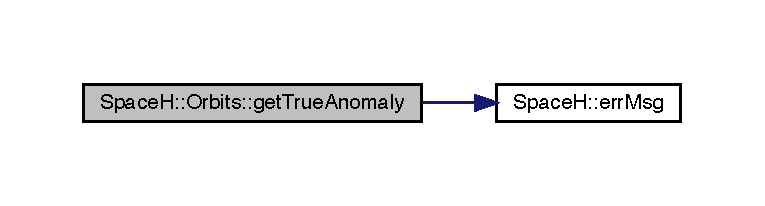
\includegraphics[width=350pt]{namespace_space_h_1_1_orbits_a43d1a07ed25eaf775f3a83d7000a2596_cgraph}
\end{center}
\end{figure}
Here is the caller graph for this function\+:
\nopagebreak
\begin{figure}[H]
\begin{center}
\leavevmode
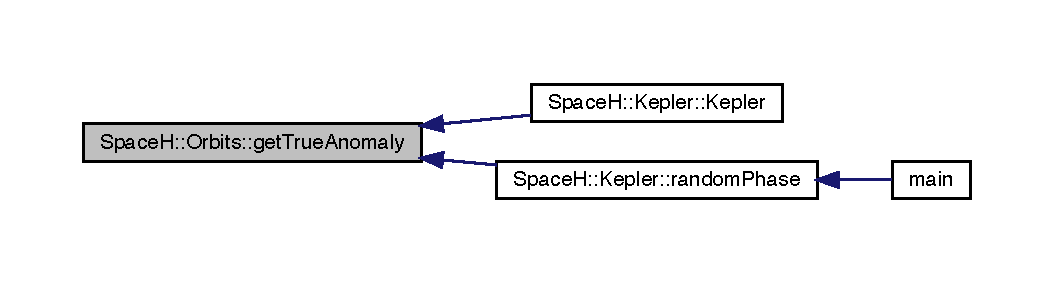
\includegraphics[width=350pt]{namespace_space_h_1_1_orbits_a43d1a07ed25eaf775f3a83d7000a2596_icgraph}
\end{center}
\end{figure}
\mbox{\Hypertarget{namespace_space_h_1_1_orbits_a678a54bbf3a8637d6437b4b8b4a39d97}\label{namespace_space_h_1_1_orbits_a678a54bbf3a8637d6437b4b8b4a39d97}} 
\index{Space\+H\+::\+Orbits@{Space\+H\+::\+Orbits}!myacos@{myacos}}
\index{myacos@{myacos}!Space\+H\+::\+Orbits@{Space\+H\+::\+Orbits}}
\subsubsection{\texorpdfstring{myacos()}{myacos()}}
{\footnotesize\ttfamily template$<$typename Scalar $>$ \\
\mbox{\hyperlink{create_kepler_8cpp_a8c2981f3f834be9448a6ab06c28748eb}{Scalar}} Space\+H\+::\+Orbits\+::myacos (\begin{DoxyParamCaption}\item[{\mbox{\hyperlink{create_kepler_8cpp_a8c2981f3f834be9448a6ab06c28748eb}{Scalar}}}]{x }\end{DoxyParamCaption})\hspace{0.3cm}{\ttfamily [inline]}}

Here is the call graph for this function\+:
\nopagebreak
\begin{figure}[H]
\begin{center}
\leavevmode
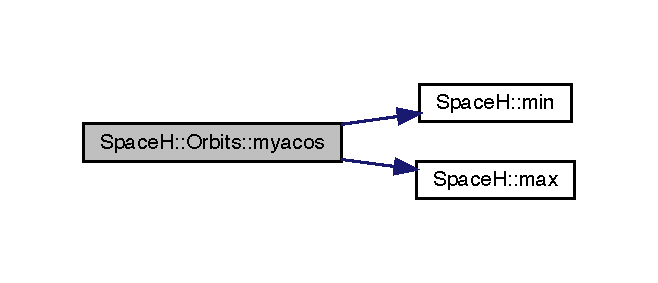
\includegraphics[width=316pt]{namespace_space_h_1_1_orbits_a678a54bbf3a8637d6437b4b8b4a39d97_cgraph}
\end{center}
\end{figure}
Here is the caller graph for this function\+:
\nopagebreak
\begin{figure}[H]
\begin{center}
\leavevmode
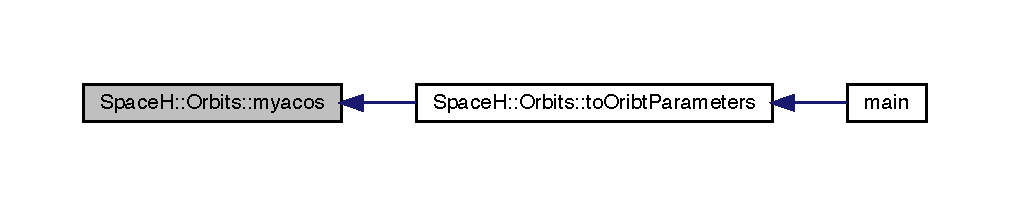
\includegraphics[width=350pt]{namespace_space_h_1_1_orbits_a678a54bbf3a8637d6437b4b8b4a39d97_icgraph}
\end{center}
\end{figure}
\mbox{\Hypertarget{namespace_space_h_1_1_orbits_a5e8b37a1237e17770907f5c2adbb53d6}\label{namespace_space_h_1_1_orbits_a5e8b37a1237e17770907f5c2adbb53d6}} 
\index{Space\+H\+::\+Orbits@{Space\+H\+::\+Orbits}!to\+Oribt\+Parameters@{to\+Oribt\+Parameters}}
\index{to\+Oribt\+Parameters@{to\+Oribt\+Parameters}!Space\+H\+::\+Orbits@{Space\+H\+::\+Orbits}}
\subsubsection{\texorpdfstring{to\+Oribt\+Parameters()}{toOribtParameters()}}
{\footnotesize\ttfamily template$<$typename Vector , typename Scalar $>$ \\
void Space\+H\+::\+Orbits\+::to\+Oribt\+Parameters (\begin{DoxyParamCaption}\item[{\mbox{\hyperlink{create_kepler_8cpp_a8c2981f3f834be9448a6ab06c28748eb}{Scalar}}}]{m1,  }\item[{\mbox{\hyperlink{create_kepler_8cpp_a8c2981f3f834be9448a6ab06c28748eb}{Scalar}}}]{m2,  }\item[{const Vector \&}]{pos1,  }\item[{const Vector \&}]{pos2,  }\item[{const Vector \&}]{vel1,  }\item[{const Vector \&}]{vel2,  }\item[{\mbox{\hyperlink{struct_space_h_1_1_orbits_1_1_param}{Param}}$<$ \mbox{\hyperlink{create_kepler_8cpp_a8c2981f3f834be9448a6ab06c28748eb}{Scalar}} $>$ \&}]{params }\end{DoxyParamCaption})\hspace{0.3cm}{\ttfamily [inline]}}

Here is the call graph for this function\+:
\nopagebreak
\begin{figure}[H]
\begin{center}
\leavevmode
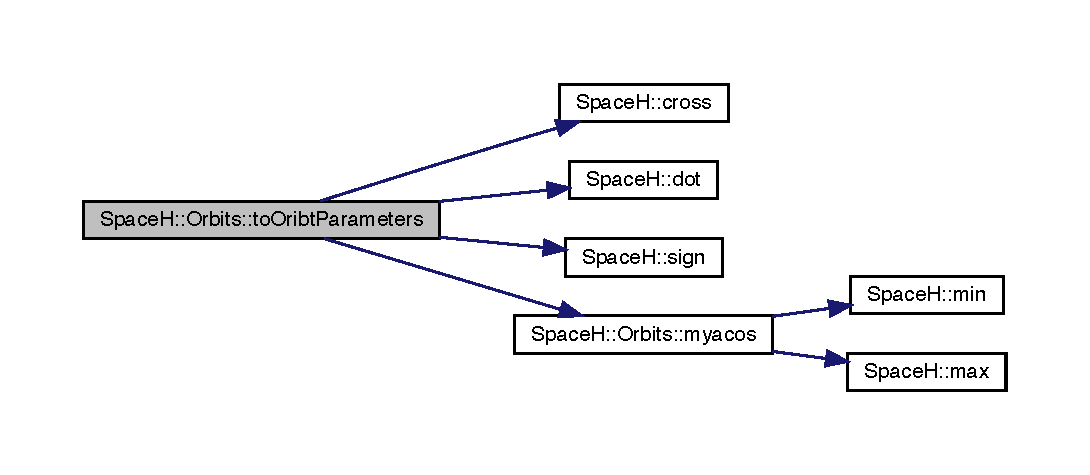
\includegraphics[width=350pt]{namespace_space_h_1_1_orbits_a5e8b37a1237e17770907f5c2adbb53d6_cgraph}
\end{center}
\end{figure}
Here is the caller graph for this function\+:
\nopagebreak
\begin{figure}[H]
\begin{center}
\leavevmode
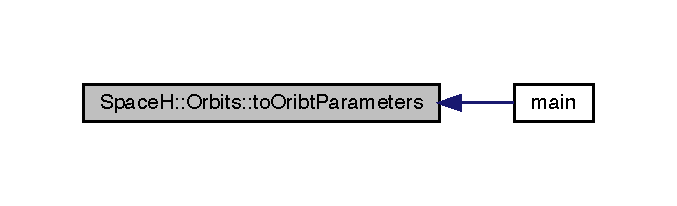
\includegraphics[width=325pt]{namespace_space_h_1_1_orbits_a5e8b37a1237e17770907f5c2adbb53d6_icgraph}
\end{center}
\end{figure}

\hypertarget{namespace_space_h_1_1_radau}{}\section{SpaceH\+:\+:Radau Namespace Reference}
\label{namespace_space_h_1_1_radau}\index{Space\+H\+::\+Radau@{Space\+H\+::\+Radau}}
\subsection*{Functions}
\begin{DoxyCompactItemize}
\item 
{\footnotesize template$<$typename Radau\+Tab $>$ }\\void \mbox{\hyperlink{namespace_space_h_1_1_radau_ac20bc7d0c1a878276e64f05506b875e5}{trans\+G2B}} (const Radau\+Tab \&G, Radau\+Tab \&B)
\end{DoxyCompactItemize}
\subsection*{Variables}
\begin{DoxyCompactItemize}
\item 
constexpr double \mbox{\hyperlink{namespace_space_h_1_1_radau_ace842233b380d237a5275cf16462ceeb}{interplt}} \mbox{[}8\mbox{]} = \{5.\+62625605369221465e-\/02, 1.\+80240691736892365e-\/01, 3.\+52624717113169637e-\/01, 5.\+47153626330555383e-\/01, 7.\+34210177215410532e-\/01, 8.\+85320946839095768e-\/01, 9.\+77520613561287502e-\/01\}
\item 
constexpr double \mbox{\hyperlink{namespace_space_h_1_1_radau_a9fb1c247de193221b47ce294964aa06b}{VC}} \mbox{[}8\mbox{]}\mbox{[}8\mbox{]}
\item 
constexpr double \mbox{\hyperlink{namespace_space_h_1_1_radau_a24cc5eaca3250fc45186dd96873afe73}{PC}} \mbox{[}8\mbox{]}\mbox{[}9\mbox{]}
\item 
constexpr double \mbox{\hyperlink{namespace_space_h_1_1_radau_a4b01e8b6450f665f02918969259eea09}{gg}} \mbox{[}28\mbox{]}
\item 
constexpr double \mbox{\hyperlink{namespace_space_h_1_1_radau_a8ef5a0de3fa20bfed420d08e5b85dcd9}{c}} \mbox{[}21\mbox{]}
\item 
constexpr double \mbox{\hyperlink{namespace_space_h_1_1_radau_aa4b3264817117df4b43f0b8a176edf69}{max\+Step\+Cof}} = 1.\+74867862159014
\item 
constexpr double \mbox{\hyperlink{namespace_space_h_1_1_radau_a4f2cef8d9622ff78d76403b062ec33a7}{min\+Step\+Cof}} = 0.\+5718603679678214
\item 
constexpr double \mbox{\hyperlink{namespace_space_h_1_1_radau_aa1696f42694bdb9870e499a1cf1068d9}{max\+Float}} = 1e100
\end{DoxyCompactItemize}


\subsection{Function Documentation}
\mbox{\Hypertarget{namespace_space_h_1_1_radau_ac20bc7d0c1a878276e64f05506b875e5}\label{namespace_space_h_1_1_radau_ac20bc7d0c1a878276e64f05506b875e5}} 
\index{Space\+H\+::\+Radau@{Space\+H\+::\+Radau}!trans\+G2B@{trans\+G2B}}
\index{trans\+G2B@{trans\+G2B}!Space\+H\+::\+Radau@{Space\+H\+::\+Radau}}
\subsubsection{\texorpdfstring{trans\+G2\+B()}{transG2B()}}
{\footnotesize\ttfamily template$<$typename Radau\+Tab $>$ \\
void Space\+H\+::\+Radau\+::trans\+G2B (\begin{DoxyParamCaption}\item[{const Radau\+Tab \&}]{G,  }\item[{Radau\+Tab \&}]{B }\end{DoxyParamCaption})}

Here is the caller graph for this function\+:
\nopagebreak
\begin{figure}[H]
\begin{center}
\leavevmode
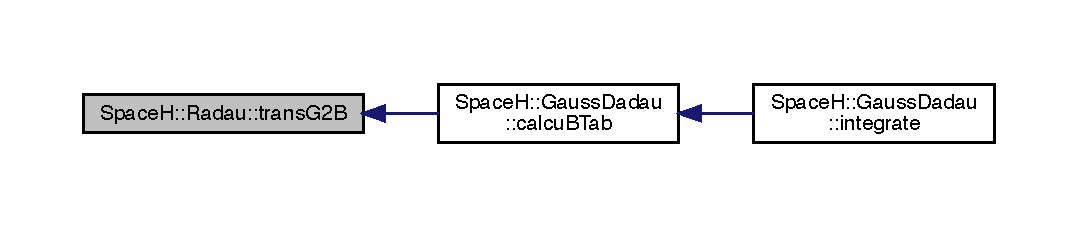
\includegraphics[width=350pt]{namespace_space_h_1_1_radau_ac20bc7d0c1a878276e64f05506b875e5_icgraph}
\end{center}
\end{figure}


\subsection{Variable Documentation}
\mbox{\Hypertarget{namespace_space_h_1_1_radau_a8ef5a0de3fa20bfed420d08e5b85dcd9}\label{namespace_space_h_1_1_radau_a8ef5a0de3fa20bfed420d08e5b85dcd9}} 
\index{Space\+H\+::\+Radau@{Space\+H\+::\+Radau}!c@{c}}
\index{c@{c}!Space\+H\+::\+Radau@{Space\+H\+::\+Radau}}
\subsubsection{\texorpdfstring{c}{c}}
{\footnotesize\ttfamily constexpr double Space\+H\+::\+Radau\+::c\mbox{[}21\mbox{]}}

{\bfseries Initial value\+:}
\begin{DoxyCode}
=
        \{
             1.27179030902686775e-03, -1.43653023637089149e-03,  1.95656540994722109e-03, -3.57589772925161
      718e-03,  1.01408028300636298e-02, -5.62625605369221488e-02,
            -3.87603579159067693e-02,  4.21585277212687057e-02, -5.47553868890686898e-02,  9.35376952594620
      670e-02, -2.36503252273814524e-01,
             3.60962243452845999e-01, -3.60099596502056807e-01,  4.15881200082306890e-01, -5.89127969386984
      196e-01,
            -1.46688420840042699e+00,  1.25015071184069093e+00, -1.13628159571753962e+00,
             2.90613625930842900e+00, -1.87049177293294999e+00,
            -2.75581271977204567e+00
        \}
\end{DoxyCode}
\mbox{\Hypertarget{namespace_space_h_1_1_radau_a4b01e8b6450f665f02918969259eea09}\label{namespace_space_h_1_1_radau_a4b01e8b6450f665f02918969259eea09}} 
\index{Space\+H\+::\+Radau@{Space\+H\+::\+Radau}!gg@{gg}}
\index{gg@{gg}!Space\+H\+::\+Radau@{Space\+H\+::\+Radau}}
\subsubsection{\texorpdfstring{gg}{gg}}
{\footnotesize\ttfamily constexpr double Space\+H\+::\+Radau\+::gg\mbox{[}28\mbox{]}}

{\bfseries Initial value\+:}
\begin{DoxyCode}
=
        \{
            1.77738089140780001e+01,
            4.47509303845559954e+01, 8.06593864838188709e+00,
            5.55095216749226992e+01, 1.95740293777069741e+01, 5.80100155926406205e+00,
            5.21625022561530086e+01, 2.85409022679298973e+01, 1.40104739330160323e+01, 5.14062410581093270e
      +00,
            5.08080910907447823e+01, 3.73038175637124453e+01, 2.52900342103279856e+01, 1.40099072392295156e
      +01, 5.34597689987110987e+00,
            7.09853803416487244e+01, 6.28448441358017857e+01, 5.21020450666394487e+01, 3.67361232269326421e
      +01, 1.95691943377340431e+01, 6.61766201370242155e+00,
            2.30858165231426693e+02, 2.25668615322657310e+02, 2.07899029180855735e+02, 1.65753721732680304e
      +02, 1.03578820531755138e+02, 4.45769049331641530e+01, 1.08460261902368476e+01
        \}
\end{DoxyCode}
\mbox{\Hypertarget{namespace_space_h_1_1_radau_ace842233b380d237a5275cf16462ceeb}\label{namespace_space_h_1_1_radau_ace842233b380d237a5275cf16462ceeb}} 
\index{Space\+H\+::\+Radau@{Space\+H\+::\+Radau}!interplt@{interplt}}
\index{interplt@{interplt}!Space\+H\+::\+Radau@{Space\+H\+::\+Radau}}
\subsubsection{\texorpdfstring{interplt}{interplt}}
{\footnotesize\ttfamily constexpr double Space\+H\+::\+Radau\+::interplt\mbox{[}8\mbox{]} = \{5.\+62625605369221465e-\/02, 1.\+80240691736892365e-\/01, 3.\+52624717113169637e-\/01, 5.\+47153626330555383e-\/01, 7.\+34210177215410532e-\/01, 8.\+85320946839095768e-\/01, 9.\+77520613561287502e-\/01\}}

Gauss radau stepping. see details in \href{https://www.cambridge.org/core/journals/international-astronomical-union-colloquium/article/an-efficient-integrator-that-uses-gauss-radau-spacings/F942BC9121C74CC2FA296050FC18D824}{\tt https\+://www.\+cambridge.\+org/core/journals/international-\/astronomical-\/union-\/colloquium/article/an-\/efficient-\/integrator-\/that-\/uses-\/gauss-\/radau-\/spacings/\+F942\+B\+C9121\+C74\+C\+C2\+F\+A296050\+F\+C18\+D824} \mbox{\Hypertarget{namespace_space_h_1_1_radau_aa1696f42694bdb9870e499a1cf1068d9}\label{namespace_space_h_1_1_radau_aa1696f42694bdb9870e499a1cf1068d9}} 
\index{Space\+H\+::\+Radau@{Space\+H\+::\+Radau}!max\+Float@{max\+Float}}
\index{max\+Float@{max\+Float}!Space\+H\+::\+Radau@{Space\+H\+::\+Radau}}
\subsubsection{\texorpdfstring{max\+Float}{maxFloat}}
{\footnotesize\ttfamily constexpr double Space\+H\+::\+Radau\+::max\+Float = 1e100}

\mbox{\Hypertarget{namespace_space_h_1_1_radau_aa4b3264817117df4b43f0b8a176edf69}\label{namespace_space_h_1_1_radau_aa4b3264817117df4b43f0b8a176edf69}} 
\index{Space\+H\+::\+Radau@{Space\+H\+::\+Radau}!max\+Step\+Cof@{max\+Step\+Cof}}
\index{max\+Step\+Cof@{max\+Step\+Cof}!Space\+H\+::\+Radau@{Space\+H\+::\+Radau}}
\subsubsection{\texorpdfstring{max\+Step\+Cof}{maxStepCof}}
{\footnotesize\ttfamily constexpr double Space\+H\+::\+Radau\+::max\+Step\+Cof = 1.\+74867862159014}

\mbox{\Hypertarget{namespace_space_h_1_1_radau_a4f2cef8d9622ff78d76403b062ec33a7}\label{namespace_space_h_1_1_radau_a4f2cef8d9622ff78d76403b062ec33a7}} 
\index{Space\+H\+::\+Radau@{Space\+H\+::\+Radau}!min\+Step\+Cof@{min\+Step\+Cof}}
\index{min\+Step\+Cof@{min\+Step\+Cof}!Space\+H\+::\+Radau@{Space\+H\+::\+Radau}}
\subsubsection{\texorpdfstring{min\+Step\+Cof}{minStepCof}}
{\footnotesize\ttfamily constexpr double Space\+H\+::\+Radau\+::min\+Step\+Cof = 0.\+5718603679678214}

\mbox{\Hypertarget{namespace_space_h_1_1_radau_a24cc5eaca3250fc45186dd96873afe73}\label{namespace_space_h_1_1_radau_a24cc5eaca3250fc45186dd96873afe73}} 
\index{Space\+H\+::\+Radau@{Space\+H\+::\+Radau}!PC@{PC}}
\index{PC@{PC}!Space\+H\+::\+Radau@{Space\+H\+::\+Radau}}
\subsubsection{\texorpdfstring{PC}{PC}}
{\footnotesize\ttfamily constexpr double Space\+H\+::\+Radau\+::\+PC\mbox{[}8\mbox{]}\mbox{[}9\mbox{]}}

{\bfseries Initial value\+:}
\begin{DoxyCode}
=
        \{
            \{5.62625605369221488e-02, 1.58273785908541475e-03, 2.96829615369572350e-05, 8.35019710194094070
      e-07, 2.81882081965910438e-08, 1.05729384672537914e-09, 4.24900421833585225e-11, 1.79294892791818847e-12, 7.
      84590314640274681e-14\},
            \{1.80240691736892361e-01, 1.62433534788967291e-02, 9.75904422387734491e-04, 8.79488440801288243
      e-05, 9.51117629667750602e-06, 1.14286732996312523e-06, 1.47136570082892073e-07, 1.98899978786506567e-08, 2.
      78832320378369023e-09\},
            \{3.52624717113169617e-01, 6.21720955595714486e-02, 7.30780586967561031e-03, 1.28845648875616128
      e-03, 2.72604962916161508e-04, 6.40848319546383638e-05, 1.61413540994638327e-05, 4.26888031736020103e-06, 1.
      17079877778820337e-06\},
            \{5.47153626330555420e-01, 1.49688545403338535e-01, 2.73008768125275573e-02, 7.46888687498911401
      e-03, 2.45197712298179009e-03, 8.94405449679365805e-04, 3.49555132287054362e-04, 1.43445268674989108e-04, 6.
      10451325053742022e-05\},
            \{7.34210177215410487e-01, 2.69532292163342236e-01, 6.59644506648410994e-02, 2.42158855062750928
      e-02, 1.06677297533941957e-02, 5.22157050181710644e-03, 2.73837871677278399e-03, 1.50790914219349057e-03, 8.
      61095074400260249e-04\},
            \{8.85320946839095790e-01, 3.91896589456036537e-01, 1.15651419880076890e-01, 5.11943122757577493
      e-02, 2.71940382100501173e-02, 1.60503011043334130e-02, 1.01497626933864586e-02, 6.73934813842577294e-03, 4.
      64060028054731337e-03\},
            \{9.77520613561287499e-01, 4.77773274968617985e-01, 1.55677741630169725e-01, 7.60891007580795496
      e-02, 4.46271986750187282e-02, 2.90826710868838558e-02, 2.03063646320370162e-02, 1.48874175107310391e-02, 1.
      13188113884477806e-02\},
            \{1.00000000000000000e+00, 5.00000000000000000e-01, 1.66666666666666667e-01, 8.33333333333333333
      e-02, 5.00000000000000000e-02, 3.33333333333333333e-02, 2.38095238095238095e-02, 1.78571428571428571e-02, 1.
      38888888888888889e-02\}
        \}
\end{DoxyCode}
\mbox{\Hypertarget{namespace_space_h_1_1_radau_a9fb1c247de193221b47ce294964aa06b}\label{namespace_space_h_1_1_radau_a9fb1c247de193221b47ce294964aa06b}} 
\index{Space\+H\+::\+Radau@{Space\+H\+::\+Radau}!VC@{VC}}
\index{VC@{VC}!Space\+H\+::\+Radau@{Space\+H\+::\+Radau}}
\subsubsection{\texorpdfstring{VC}{VC}}
{\footnotesize\ttfamily constexpr double Space\+H\+::\+Radau\+::\+VC\mbox{[}8\mbox{]}\mbox{[}8\mbox{]}}

{\bfseries Initial value\+:}
\begin{DoxyCode}
=
        \{
            \{5.62625605369221488e-02, 1.58273785908541475e-03, 5.93659230739144700e-05, 2.50505913058228221
      e-06, 1.12752832786364175e-07, 5.28646923362689570e-09, 2.54940253100151135e-10, 1.25506424954273193e-11\},
            \{1.80240691736892361e-01, 1.62433534788967291e-02, 1.95180884477546898e-03, 2.63846532240386473
      e-04, 3.80447051867100241e-05, 5.71433664981562616e-06, 8.82819420497352435e-07, 1.39229985150554597e-07\},
            \{3.52624717113169617e-01, 6.21720955595714486e-02, 1.46156117393512206e-02, 3.86536946626848384
      e-03, 1.09041985166464603e-03, 3.20424159773191819e-04, 9.68481245967829960e-05, 2.98821622215214072e-05\},
            \{5.47153626330555420e-01, 1.49688545403338535e-01, 5.46017536250551146e-02, 2.24066606249673420
      e-02, 9.80790849192716036e-03, 4.47202724839682903e-03, 2.09733079372232617e-03, 1.00411688072492376e-03\},
            \{7.34210177215410487e-01, 2.69532292163342236e-01, 1.31928901329682199e-01, 7.26476565188252785
      e-02, 4.26709190135767829e-02, 2.61078525090855322e-02, 1.64302723006367039e-02, 1.05553639953544340e-02\},
            \{8.85320946839095790e-01, 3.91896589456036537e-01, 2.31302839760153781e-01, 1.53582936827273248
      e-01, 1.08776152840200469e-01, 8.02515055216670650e-02, 6.08985761603187514e-02, 4.71754369689804106e-02\},
            \{9.77520613561287499e-01, 4.77773274968617985e-01, 3.11355483260339450e-01, 2.28267302274238649
      e-01, 1.78508794700074913e-01, 1.45413355434419279e-01, 1.21838187792222097e-01, 1.04211922575117274e-01\},
            \{1.00000000000000000e+00, 5.00000000000000000e-01, 3.33333333333333333e-01, 2.50000000000000000
      e-01, 2.00000000000000000e-01, 1.66666666666666667e-01, 1.42857142857142857e-01, 1.25000000000000000e-01\}
        \}
\end{DoxyCode}

\hypertarget{namespace_space_h_1_1_unit}{}\section{SpaceH\+:\+:Unit Namespace Reference}
\label{namespace_space_h_1_1_unit}\index{Space\+H\+::\+Unit@{Space\+H\+::\+Unit}}
\subsection*{Variables}
\begin{DoxyCompactItemize}
\item 
constexpr double \mbox{\hyperlink{namespace_space_h_1_1_unit_a3851fdb2c14e9823ba0a46b68f99d6f9}{AU}} = 1
\item 
constexpr double \mbox{\hyperlink{namespace_space_h_1_1_unit_a65df0928124a0990520fda009dbfd3e4}{M\+\_\+\+S\+O\+L\+AR}} = 1
\item 
constexpr double \mbox{\hyperlink{namespace_space_h_1_1_unit_a386ecd4744a86ce94e14270b1305fc62}{Y\+E\+AR}} = 2$\ast$\mbox{\hyperlink{namespace_space_h_1_1_const_afdcc70c6f78ec4cf7baad3525ba7c618}{Const\+::\+PI}}
\item 
constexpr double \mbox{\hyperlink{namespace_space_h_1_1_unit_a92db3086d9b968f2931b81b4c31cf587}{K\+YR}} = 1e3$\ast$\+Y\+E\+AR
\item 
constexpr double \mbox{\hyperlink{namespace_space_h_1_1_unit_a6d4784385a7314879a24cf69b8e0d434}{M\+YR}} = 1e6$\ast$\+Y\+E\+AR
\item 
constexpr double \mbox{\hyperlink{namespace_space_h_1_1_unit_a41d9004e5902ee96826af6512c6819c4}{G\+YR}} = 1e9$\ast$\+Y\+E\+AR
\item 
constexpr double \mbox{\hyperlink{namespace_space_h_1_1_unit_ad38d8884159cb621872ee7587073b529}{M\+O\+N\+TH}} = \mbox{\hyperlink{namespace_space_h_1_1_unit_a386ecd4744a86ce94e14270b1305fc62}{Y\+E\+AR}} / 12
\item 
constexpr double \mbox{\hyperlink{namespace_space_h_1_1_unit_a1f85dcd972f4336bccee277f6bb2654c}{D\+AY}} = \mbox{\hyperlink{namespace_space_h_1_1_unit_a386ecd4744a86ce94e14270b1305fc62}{Y\+E\+AR}} / 365.\+25636042
\item 
constexpr double \mbox{\hyperlink{namespace_space_h_1_1_unit_a3a80e4b127a3d63688a18077d0d47bee}{H\+O\+UR}} = \mbox{\hyperlink{namespace_space_h_1_1_unit_a1f85dcd972f4336bccee277f6bb2654c}{D\+AY}} / 24
\item 
constexpr double \mbox{\hyperlink{namespace_space_h_1_1_unit_a581da52233fafb94663eb4e8377b4b5a}{M\+I\+N\+U\+TE}} = \mbox{\hyperlink{namespace_space_h_1_1_unit_a3a80e4b127a3d63688a18077d0d47bee}{H\+O\+UR}} / 60
\item 
constexpr double \mbox{\hyperlink{namespace_space_h_1_1_unit_a3ece158d89b3558ae66acd7e5324a101}{S\+E\+C\+O\+ND}} = \mbox{\hyperlink{namespace_space_h_1_1_unit_a581da52233fafb94663eb4e8377b4b5a}{M\+I\+N\+U\+TE}} /60
\item 
constexpr double \mbox{\hyperlink{namespace_space_h_1_1_unit_af26bad8094a2c37c5b9932d9c40baaac}{H\+U\+B\+B\+L\+E\+T\+I\+ME}} = 14.\+7$\ast$\mbox{\hyperlink{namespace_space_h_1_1_unit_a41d9004e5902ee96826af6512c6819c4}{G\+YR}}
\item 
constexpr double \mbox{\hyperlink{namespace_space_h_1_1_unit_a57affbb952358107b4b23bfe8b2bcd6b}{KM}} = 1 / 149597870.\+7
\item 
constexpr double \mbox{\hyperlink{namespace_space_h_1_1_unit_ac3a4adce0bc40c23ec0c3abfa48292ff}{PC}} = 648000/\mbox{\hyperlink{namespace_space_h_1_1_const_afdcc70c6f78ec4cf7baad3525ba7c618}{Const\+::\+PI}}
\item 
constexpr double \mbox{\hyperlink{namespace_space_h_1_1_unit_a0808076f6fe0cac6268f660dd72c6458}{R\+\_\+\+S\+O\+L\+AR}} = 6.\+957\+E5$\ast$\+KM
\item 
constexpr double \mbox{\hyperlink{namespace_space_h_1_1_unit_af411a7d1df0c45c90d4f2e23fd96de94}{M\+\_\+\+E\+A\+R\+TH}} = 3.\+003\+E-\/6$\ast$\+M\+\_\+\+S\+O\+L\+AR
\item 
constexpr double \mbox{\hyperlink{namespace_space_h_1_1_unit_a36faff1fcf3f6090c74d2e96aea6ad9c}{M\+\_\+\+M\+E\+C\+U\+RY}} = 0.\+055$\ast$\mbox{\hyperlink{namespace_space_h_1_1_unit_af411a7d1df0c45c90d4f2e23fd96de94}{M\+\_\+\+E\+A\+R\+TH}}
\item 
constexpr double \mbox{\hyperlink{namespace_space_h_1_1_unit_a7a668de567b17096cdc91a81403f7347}{M\+\_\+\+V\+E\+N\+US}} = 0.\+815$\ast$\mbox{\hyperlink{namespace_space_h_1_1_unit_af411a7d1df0c45c90d4f2e23fd96de94}{M\+\_\+\+E\+A\+R\+TH}}
\item 
constexpr double \mbox{\hyperlink{namespace_space_h_1_1_unit_a8d04d7cdfd1d857c8b6e633edc6998e7}{M\+\_\+\+M\+A\+RS}} = 0.\+107$\ast$\mbox{\hyperlink{namespace_space_h_1_1_unit_af411a7d1df0c45c90d4f2e23fd96de94}{M\+\_\+\+E\+A\+R\+TH}}
\item 
constexpr double \mbox{\hyperlink{namespace_space_h_1_1_unit_a7cfce92c7e60f385723a1bfb8cfd4c75}{M\+\_\+\+J\+U\+P\+I\+T\+ER}} = 317.\+8$\ast$\mbox{\hyperlink{namespace_space_h_1_1_unit_af411a7d1df0c45c90d4f2e23fd96de94}{M\+\_\+\+E\+A\+R\+TH}}
\item 
constexpr double \mbox{\hyperlink{namespace_space_h_1_1_unit_aea9be6aefe6f65546fc195c0e4748ca4}{M\+\_\+\+S\+A\+T\+U\+RN}} = 95.\+16$\ast$\mbox{\hyperlink{namespace_space_h_1_1_unit_af411a7d1df0c45c90d4f2e23fd96de94}{M\+\_\+\+E\+A\+R\+TH}}
\item 
constexpr double \mbox{\hyperlink{namespace_space_h_1_1_unit_aa5e34a70455ece7b0d0461b2100d2e37}{M\+\_\+\+N\+E\+P\+T\+U\+NE}} = 17.\+15$\ast$\mbox{\hyperlink{namespace_space_h_1_1_unit_af411a7d1df0c45c90d4f2e23fd96de94}{M\+\_\+\+E\+A\+R\+TH}}
\item 
constexpr double \mbox{\hyperlink{namespace_space_h_1_1_unit_a06ca6cd52ca75780258cbe237788d27c}{M\+\_\+\+M\+O\+ON}} = 0.\+012300$\ast$\mbox{\hyperlink{namespace_space_h_1_1_unit_af411a7d1df0c45c90d4f2e23fd96de94}{M\+\_\+\+E\+A\+R\+TH}}
\item 
constexpr double \mbox{\hyperlink{namespace_space_h_1_1_unit_a08a0bb62e0888ec690dd0e70a415e3fb}{V\+\_\+\+U\+N\+IT}} = 2.\+9784651272402163\+E1
\item 
constexpr double \mbox{\hyperlink{namespace_space_h_1_1_unit_a94c0a976eb50dcc88f04f3513049e8c3}{K\+MS}} = 1 / \mbox{\hyperlink{namespace_space_h_1_1_unit_a08a0bb62e0888ec690dd0e70a415e3fb}{V\+\_\+\+U\+N\+IT}}
\item 
constexpr double \mbox{\hyperlink{namespace_space_h_1_1_unit_ad18c80501bf460d50d363aecc5d933e8}{D\+EG}} = \mbox{\hyperlink{namespace_space_h_1_1_const_afdcc70c6f78ec4cf7baad3525ba7c618}{Const\+::\+PI}}/180
\end{DoxyCompactItemize}


\subsection{Variable Documentation}
\mbox{\Hypertarget{namespace_space_h_1_1_unit_a3851fdb2c14e9823ba0a46b68f99d6f9}\label{namespace_space_h_1_1_unit_a3851fdb2c14e9823ba0a46b68f99d6f9}} 
\index{Space\+H\+::\+Unit@{Space\+H\+::\+Unit}!AU@{AU}}
\index{AU@{AU}!Space\+H\+::\+Unit@{Space\+H\+::\+Unit}}
\subsubsection{\texorpdfstring{AU}{AU}}
{\footnotesize\ttfamily constexpr double Space\+H\+::\+Unit\+::\+AU = 1}

\mbox{\Hypertarget{namespace_space_h_1_1_unit_a1f85dcd972f4336bccee277f6bb2654c}\label{namespace_space_h_1_1_unit_a1f85dcd972f4336bccee277f6bb2654c}} 
\index{Space\+H\+::\+Unit@{Space\+H\+::\+Unit}!D\+AY@{D\+AY}}
\index{D\+AY@{D\+AY}!Space\+H\+::\+Unit@{Space\+H\+::\+Unit}}
\subsubsection{\texorpdfstring{D\+AY}{DAY}}
{\footnotesize\ttfamily constexpr double Space\+H\+::\+Unit\+::\+D\+AY = \mbox{\hyperlink{namespace_space_h_1_1_unit_a386ecd4744a86ce94e14270b1305fc62}{Y\+E\+AR}} / 365.\+25636042}

\mbox{\Hypertarget{namespace_space_h_1_1_unit_ad18c80501bf460d50d363aecc5d933e8}\label{namespace_space_h_1_1_unit_ad18c80501bf460d50d363aecc5d933e8}} 
\index{Space\+H\+::\+Unit@{Space\+H\+::\+Unit}!D\+EG@{D\+EG}}
\index{D\+EG@{D\+EG}!Space\+H\+::\+Unit@{Space\+H\+::\+Unit}}
\subsubsection{\texorpdfstring{D\+EG}{DEG}}
{\footnotesize\ttfamily constexpr double Space\+H\+::\+Unit\+::\+D\+EG = \mbox{\hyperlink{namespace_space_h_1_1_const_afdcc70c6f78ec4cf7baad3525ba7c618}{Const\+::\+PI}}/180}

\mbox{\Hypertarget{namespace_space_h_1_1_unit_a41d9004e5902ee96826af6512c6819c4}\label{namespace_space_h_1_1_unit_a41d9004e5902ee96826af6512c6819c4}} 
\index{Space\+H\+::\+Unit@{Space\+H\+::\+Unit}!G\+YR@{G\+YR}}
\index{G\+YR@{G\+YR}!Space\+H\+::\+Unit@{Space\+H\+::\+Unit}}
\subsubsection{\texorpdfstring{G\+YR}{GYR}}
{\footnotesize\ttfamily constexpr double Space\+H\+::\+Unit\+::\+G\+YR = 1e9$\ast$\+Y\+E\+AR}

\mbox{\Hypertarget{namespace_space_h_1_1_unit_a3a80e4b127a3d63688a18077d0d47bee}\label{namespace_space_h_1_1_unit_a3a80e4b127a3d63688a18077d0d47bee}} 
\index{Space\+H\+::\+Unit@{Space\+H\+::\+Unit}!H\+O\+UR@{H\+O\+UR}}
\index{H\+O\+UR@{H\+O\+UR}!Space\+H\+::\+Unit@{Space\+H\+::\+Unit}}
\subsubsection{\texorpdfstring{H\+O\+UR}{HOUR}}
{\footnotesize\ttfamily constexpr double Space\+H\+::\+Unit\+::\+H\+O\+UR = \mbox{\hyperlink{namespace_space_h_1_1_unit_a1f85dcd972f4336bccee277f6bb2654c}{D\+AY}} / 24}

\mbox{\Hypertarget{namespace_space_h_1_1_unit_af26bad8094a2c37c5b9932d9c40baaac}\label{namespace_space_h_1_1_unit_af26bad8094a2c37c5b9932d9c40baaac}} 
\index{Space\+H\+::\+Unit@{Space\+H\+::\+Unit}!H\+U\+B\+B\+L\+E\+T\+I\+ME@{H\+U\+B\+B\+L\+E\+T\+I\+ME}}
\index{H\+U\+B\+B\+L\+E\+T\+I\+ME@{H\+U\+B\+B\+L\+E\+T\+I\+ME}!Space\+H\+::\+Unit@{Space\+H\+::\+Unit}}
\subsubsection{\texorpdfstring{H\+U\+B\+B\+L\+E\+T\+I\+ME}{HUBBLETIME}}
{\footnotesize\ttfamily constexpr double Space\+H\+::\+Unit\+::\+H\+U\+B\+B\+L\+E\+T\+I\+ME = 14.\+7$\ast$\mbox{\hyperlink{namespace_space_h_1_1_unit_a41d9004e5902ee96826af6512c6819c4}{G\+YR}}}

\mbox{\Hypertarget{namespace_space_h_1_1_unit_a57affbb952358107b4b23bfe8b2bcd6b}\label{namespace_space_h_1_1_unit_a57affbb952358107b4b23bfe8b2bcd6b}} 
\index{Space\+H\+::\+Unit@{Space\+H\+::\+Unit}!KM@{KM}}
\index{KM@{KM}!Space\+H\+::\+Unit@{Space\+H\+::\+Unit}}
\subsubsection{\texorpdfstring{KM}{KM}}
{\footnotesize\ttfamily constexpr double Space\+H\+::\+Unit\+::\+KM = 1 / 149597870.\+7}

\mbox{\Hypertarget{namespace_space_h_1_1_unit_a94c0a976eb50dcc88f04f3513049e8c3}\label{namespace_space_h_1_1_unit_a94c0a976eb50dcc88f04f3513049e8c3}} 
\index{Space\+H\+::\+Unit@{Space\+H\+::\+Unit}!K\+MS@{K\+MS}}
\index{K\+MS@{K\+MS}!Space\+H\+::\+Unit@{Space\+H\+::\+Unit}}
\subsubsection{\texorpdfstring{K\+MS}{KMS}}
{\footnotesize\ttfamily constexpr double Space\+H\+::\+Unit\+::\+K\+MS = 1 / \mbox{\hyperlink{namespace_space_h_1_1_unit_a08a0bb62e0888ec690dd0e70a415e3fb}{V\+\_\+\+U\+N\+IT}}}

\mbox{\Hypertarget{namespace_space_h_1_1_unit_a92db3086d9b968f2931b81b4c31cf587}\label{namespace_space_h_1_1_unit_a92db3086d9b968f2931b81b4c31cf587}} 
\index{Space\+H\+::\+Unit@{Space\+H\+::\+Unit}!K\+YR@{K\+YR}}
\index{K\+YR@{K\+YR}!Space\+H\+::\+Unit@{Space\+H\+::\+Unit}}
\subsubsection{\texorpdfstring{K\+YR}{KYR}}
{\footnotesize\ttfamily constexpr double Space\+H\+::\+Unit\+::\+K\+YR = 1e3$\ast$\+Y\+E\+AR}

\mbox{\Hypertarget{namespace_space_h_1_1_unit_af411a7d1df0c45c90d4f2e23fd96de94}\label{namespace_space_h_1_1_unit_af411a7d1df0c45c90d4f2e23fd96de94}} 
\index{Space\+H\+::\+Unit@{Space\+H\+::\+Unit}!M\+\_\+\+E\+A\+R\+TH@{M\+\_\+\+E\+A\+R\+TH}}
\index{M\+\_\+\+E\+A\+R\+TH@{M\+\_\+\+E\+A\+R\+TH}!Space\+H\+::\+Unit@{Space\+H\+::\+Unit}}
\subsubsection{\texorpdfstring{M\+\_\+\+E\+A\+R\+TH}{M\_EARTH}}
{\footnotesize\ttfamily constexpr double Space\+H\+::\+Unit\+::\+M\+\_\+\+E\+A\+R\+TH = 3.\+003\+E-\/6$\ast$\+M\+\_\+\+S\+O\+L\+AR}

\mbox{\Hypertarget{namespace_space_h_1_1_unit_a7cfce92c7e60f385723a1bfb8cfd4c75}\label{namespace_space_h_1_1_unit_a7cfce92c7e60f385723a1bfb8cfd4c75}} 
\index{Space\+H\+::\+Unit@{Space\+H\+::\+Unit}!M\+\_\+\+J\+U\+P\+I\+T\+ER@{M\+\_\+\+J\+U\+P\+I\+T\+ER}}
\index{M\+\_\+\+J\+U\+P\+I\+T\+ER@{M\+\_\+\+J\+U\+P\+I\+T\+ER}!Space\+H\+::\+Unit@{Space\+H\+::\+Unit}}
\subsubsection{\texorpdfstring{M\+\_\+\+J\+U\+P\+I\+T\+ER}{M\_JUPITER}}
{\footnotesize\ttfamily constexpr double Space\+H\+::\+Unit\+::\+M\+\_\+\+J\+U\+P\+I\+T\+ER = 317.\+8$\ast$\mbox{\hyperlink{namespace_space_h_1_1_unit_af411a7d1df0c45c90d4f2e23fd96de94}{M\+\_\+\+E\+A\+R\+TH}}}

\mbox{\Hypertarget{namespace_space_h_1_1_unit_a8d04d7cdfd1d857c8b6e633edc6998e7}\label{namespace_space_h_1_1_unit_a8d04d7cdfd1d857c8b6e633edc6998e7}} 
\index{Space\+H\+::\+Unit@{Space\+H\+::\+Unit}!M\+\_\+\+M\+A\+RS@{M\+\_\+\+M\+A\+RS}}
\index{M\+\_\+\+M\+A\+RS@{M\+\_\+\+M\+A\+RS}!Space\+H\+::\+Unit@{Space\+H\+::\+Unit}}
\subsubsection{\texorpdfstring{M\+\_\+\+M\+A\+RS}{M\_MARS}}
{\footnotesize\ttfamily constexpr double Space\+H\+::\+Unit\+::\+M\+\_\+\+M\+A\+RS = 0.\+107$\ast$\mbox{\hyperlink{namespace_space_h_1_1_unit_af411a7d1df0c45c90d4f2e23fd96de94}{M\+\_\+\+E\+A\+R\+TH}}}

\mbox{\Hypertarget{namespace_space_h_1_1_unit_a36faff1fcf3f6090c74d2e96aea6ad9c}\label{namespace_space_h_1_1_unit_a36faff1fcf3f6090c74d2e96aea6ad9c}} 
\index{Space\+H\+::\+Unit@{Space\+H\+::\+Unit}!M\+\_\+\+M\+E\+C\+U\+RY@{M\+\_\+\+M\+E\+C\+U\+RY}}
\index{M\+\_\+\+M\+E\+C\+U\+RY@{M\+\_\+\+M\+E\+C\+U\+RY}!Space\+H\+::\+Unit@{Space\+H\+::\+Unit}}
\subsubsection{\texorpdfstring{M\+\_\+\+M\+E\+C\+U\+RY}{M\_MECURY}}
{\footnotesize\ttfamily constexpr double Space\+H\+::\+Unit\+::\+M\+\_\+\+M\+E\+C\+U\+RY = 0.\+055$\ast$\mbox{\hyperlink{namespace_space_h_1_1_unit_af411a7d1df0c45c90d4f2e23fd96de94}{M\+\_\+\+E\+A\+R\+TH}}}

\mbox{\Hypertarget{namespace_space_h_1_1_unit_a06ca6cd52ca75780258cbe237788d27c}\label{namespace_space_h_1_1_unit_a06ca6cd52ca75780258cbe237788d27c}} 
\index{Space\+H\+::\+Unit@{Space\+H\+::\+Unit}!M\+\_\+\+M\+O\+ON@{M\+\_\+\+M\+O\+ON}}
\index{M\+\_\+\+M\+O\+ON@{M\+\_\+\+M\+O\+ON}!Space\+H\+::\+Unit@{Space\+H\+::\+Unit}}
\subsubsection{\texorpdfstring{M\+\_\+\+M\+O\+ON}{M\_MOON}}
{\footnotesize\ttfamily constexpr double Space\+H\+::\+Unit\+::\+M\+\_\+\+M\+O\+ON = 0.\+012300$\ast$\mbox{\hyperlink{namespace_space_h_1_1_unit_af411a7d1df0c45c90d4f2e23fd96de94}{M\+\_\+\+E\+A\+R\+TH}}}

\mbox{\Hypertarget{namespace_space_h_1_1_unit_aa5e34a70455ece7b0d0461b2100d2e37}\label{namespace_space_h_1_1_unit_aa5e34a70455ece7b0d0461b2100d2e37}} 
\index{Space\+H\+::\+Unit@{Space\+H\+::\+Unit}!M\+\_\+\+N\+E\+P\+T\+U\+NE@{M\+\_\+\+N\+E\+P\+T\+U\+NE}}
\index{M\+\_\+\+N\+E\+P\+T\+U\+NE@{M\+\_\+\+N\+E\+P\+T\+U\+NE}!Space\+H\+::\+Unit@{Space\+H\+::\+Unit}}
\subsubsection{\texorpdfstring{M\+\_\+\+N\+E\+P\+T\+U\+NE}{M\_NEPTUNE}}
{\footnotesize\ttfamily constexpr double Space\+H\+::\+Unit\+::\+M\+\_\+\+N\+E\+P\+T\+U\+NE = 17.\+15$\ast$\mbox{\hyperlink{namespace_space_h_1_1_unit_af411a7d1df0c45c90d4f2e23fd96de94}{M\+\_\+\+E\+A\+R\+TH}}}

\mbox{\Hypertarget{namespace_space_h_1_1_unit_aea9be6aefe6f65546fc195c0e4748ca4}\label{namespace_space_h_1_1_unit_aea9be6aefe6f65546fc195c0e4748ca4}} 
\index{Space\+H\+::\+Unit@{Space\+H\+::\+Unit}!M\+\_\+\+S\+A\+T\+U\+RN@{M\+\_\+\+S\+A\+T\+U\+RN}}
\index{M\+\_\+\+S\+A\+T\+U\+RN@{M\+\_\+\+S\+A\+T\+U\+RN}!Space\+H\+::\+Unit@{Space\+H\+::\+Unit}}
\subsubsection{\texorpdfstring{M\+\_\+\+S\+A\+T\+U\+RN}{M\_SATURN}}
{\footnotesize\ttfamily constexpr double Space\+H\+::\+Unit\+::\+M\+\_\+\+S\+A\+T\+U\+RN = 95.\+16$\ast$\mbox{\hyperlink{namespace_space_h_1_1_unit_af411a7d1df0c45c90d4f2e23fd96de94}{M\+\_\+\+E\+A\+R\+TH}}}

\mbox{\Hypertarget{namespace_space_h_1_1_unit_a65df0928124a0990520fda009dbfd3e4}\label{namespace_space_h_1_1_unit_a65df0928124a0990520fda009dbfd3e4}} 
\index{Space\+H\+::\+Unit@{Space\+H\+::\+Unit}!M\+\_\+\+S\+O\+L\+AR@{M\+\_\+\+S\+O\+L\+AR}}
\index{M\+\_\+\+S\+O\+L\+AR@{M\+\_\+\+S\+O\+L\+AR}!Space\+H\+::\+Unit@{Space\+H\+::\+Unit}}
\subsubsection{\texorpdfstring{M\+\_\+\+S\+O\+L\+AR}{M\_SOLAR}}
{\footnotesize\ttfamily constexpr double Space\+H\+::\+Unit\+::\+M\+\_\+\+S\+O\+L\+AR = 1}

\mbox{\Hypertarget{namespace_space_h_1_1_unit_a7a668de567b17096cdc91a81403f7347}\label{namespace_space_h_1_1_unit_a7a668de567b17096cdc91a81403f7347}} 
\index{Space\+H\+::\+Unit@{Space\+H\+::\+Unit}!M\+\_\+\+V\+E\+N\+US@{M\+\_\+\+V\+E\+N\+US}}
\index{M\+\_\+\+V\+E\+N\+US@{M\+\_\+\+V\+E\+N\+US}!Space\+H\+::\+Unit@{Space\+H\+::\+Unit}}
\subsubsection{\texorpdfstring{M\+\_\+\+V\+E\+N\+US}{M\_VENUS}}
{\footnotesize\ttfamily constexpr double Space\+H\+::\+Unit\+::\+M\+\_\+\+V\+E\+N\+US = 0.\+815$\ast$\mbox{\hyperlink{namespace_space_h_1_1_unit_af411a7d1df0c45c90d4f2e23fd96de94}{M\+\_\+\+E\+A\+R\+TH}}}

\mbox{\Hypertarget{namespace_space_h_1_1_unit_a581da52233fafb94663eb4e8377b4b5a}\label{namespace_space_h_1_1_unit_a581da52233fafb94663eb4e8377b4b5a}} 
\index{Space\+H\+::\+Unit@{Space\+H\+::\+Unit}!M\+I\+N\+U\+TE@{M\+I\+N\+U\+TE}}
\index{M\+I\+N\+U\+TE@{M\+I\+N\+U\+TE}!Space\+H\+::\+Unit@{Space\+H\+::\+Unit}}
\subsubsection{\texorpdfstring{M\+I\+N\+U\+TE}{MINUTE}}
{\footnotesize\ttfamily constexpr double Space\+H\+::\+Unit\+::\+M\+I\+N\+U\+TE = \mbox{\hyperlink{namespace_space_h_1_1_unit_a3a80e4b127a3d63688a18077d0d47bee}{H\+O\+UR}} / 60}

\mbox{\Hypertarget{namespace_space_h_1_1_unit_ad38d8884159cb621872ee7587073b529}\label{namespace_space_h_1_1_unit_ad38d8884159cb621872ee7587073b529}} 
\index{Space\+H\+::\+Unit@{Space\+H\+::\+Unit}!M\+O\+N\+TH@{M\+O\+N\+TH}}
\index{M\+O\+N\+TH@{M\+O\+N\+TH}!Space\+H\+::\+Unit@{Space\+H\+::\+Unit}}
\subsubsection{\texorpdfstring{M\+O\+N\+TH}{MONTH}}
{\footnotesize\ttfamily constexpr double Space\+H\+::\+Unit\+::\+M\+O\+N\+TH = \mbox{\hyperlink{namespace_space_h_1_1_unit_a386ecd4744a86ce94e14270b1305fc62}{Y\+E\+AR}} / 12}

\mbox{\Hypertarget{namespace_space_h_1_1_unit_a6d4784385a7314879a24cf69b8e0d434}\label{namespace_space_h_1_1_unit_a6d4784385a7314879a24cf69b8e0d434}} 
\index{Space\+H\+::\+Unit@{Space\+H\+::\+Unit}!M\+YR@{M\+YR}}
\index{M\+YR@{M\+YR}!Space\+H\+::\+Unit@{Space\+H\+::\+Unit}}
\subsubsection{\texorpdfstring{M\+YR}{MYR}}
{\footnotesize\ttfamily constexpr double Space\+H\+::\+Unit\+::\+M\+YR = 1e6$\ast$\+Y\+E\+AR}

\mbox{\Hypertarget{namespace_space_h_1_1_unit_ac3a4adce0bc40c23ec0c3abfa48292ff}\label{namespace_space_h_1_1_unit_ac3a4adce0bc40c23ec0c3abfa48292ff}} 
\index{Space\+H\+::\+Unit@{Space\+H\+::\+Unit}!PC@{PC}}
\index{PC@{PC}!Space\+H\+::\+Unit@{Space\+H\+::\+Unit}}
\subsubsection{\texorpdfstring{PC}{PC}}
{\footnotesize\ttfamily constexpr double Space\+H\+::\+Unit\+::\+PC = 648000/\mbox{\hyperlink{namespace_space_h_1_1_const_afdcc70c6f78ec4cf7baad3525ba7c618}{Const\+::\+PI}}}

\mbox{\Hypertarget{namespace_space_h_1_1_unit_a0808076f6fe0cac6268f660dd72c6458}\label{namespace_space_h_1_1_unit_a0808076f6fe0cac6268f660dd72c6458}} 
\index{Space\+H\+::\+Unit@{Space\+H\+::\+Unit}!R\+\_\+\+S\+O\+L\+AR@{R\+\_\+\+S\+O\+L\+AR}}
\index{R\+\_\+\+S\+O\+L\+AR@{R\+\_\+\+S\+O\+L\+AR}!Space\+H\+::\+Unit@{Space\+H\+::\+Unit}}
\subsubsection{\texorpdfstring{R\+\_\+\+S\+O\+L\+AR}{R\_SOLAR}}
{\footnotesize\ttfamily constexpr double Space\+H\+::\+Unit\+::\+R\+\_\+\+S\+O\+L\+AR = 6.\+957\+E5$\ast$\+KM}

\mbox{\Hypertarget{namespace_space_h_1_1_unit_a3ece158d89b3558ae66acd7e5324a101}\label{namespace_space_h_1_1_unit_a3ece158d89b3558ae66acd7e5324a101}} 
\index{Space\+H\+::\+Unit@{Space\+H\+::\+Unit}!S\+E\+C\+O\+ND@{S\+E\+C\+O\+ND}}
\index{S\+E\+C\+O\+ND@{S\+E\+C\+O\+ND}!Space\+H\+::\+Unit@{Space\+H\+::\+Unit}}
\subsubsection{\texorpdfstring{S\+E\+C\+O\+ND}{SECOND}}
{\footnotesize\ttfamily constexpr double Space\+H\+::\+Unit\+::\+S\+E\+C\+O\+ND = \mbox{\hyperlink{namespace_space_h_1_1_unit_a581da52233fafb94663eb4e8377b4b5a}{M\+I\+N\+U\+TE}} /60}

\mbox{\Hypertarget{namespace_space_h_1_1_unit_a08a0bb62e0888ec690dd0e70a415e3fb}\label{namespace_space_h_1_1_unit_a08a0bb62e0888ec690dd0e70a415e3fb}} 
\index{Space\+H\+::\+Unit@{Space\+H\+::\+Unit}!V\+\_\+\+U\+N\+IT@{V\+\_\+\+U\+N\+IT}}
\index{V\+\_\+\+U\+N\+IT@{V\+\_\+\+U\+N\+IT}!Space\+H\+::\+Unit@{Space\+H\+::\+Unit}}
\subsubsection{\texorpdfstring{V\+\_\+\+U\+N\+IT}{V\_UNIT}}
{\footnotesize\ttfamily constexpr double Space\+H\+::\+Unit\+::\+V\+\_\+\+U\+N\+IT = 2.\+9784651272402163\+E1}

\mbox{\Hypertarget{namespace_space_h_1_1_unit_a386ecd4744a86ce94e14270b1305fc62}\label{namespace_space_h_1_1_unit_a386ecd4744a86ce94e14270b1305fc62}} 
\index{Space\+H\+::\+Unit@{Space\+H\+::\+Unit}!Y\+E\+AR@{Y\+E\+AR}}
\index{Y\+E\+AR@{Y\+E\+AR}!Space\+H\+::\+Unit@{Space\+H\+::\+Unit}}
\subsubsection{\texorpdfstring{Y\+E\+AR}{YEAR}}
{\footnotesize\ttfamily constexpr double Space\+H\+::\+Unit\+::\+Y\+E\+AR = 2$\ast$\mbox{\hyperlink{namespace_space_h_1_1_const_afdcc70c6f78ec4cf7baad3525ba7c618}{Const\+::\+PI}}}


\chapter{Class Documentation}
\hypertarget{class_space_h_1_1_a_rchain_system}{}\section{SpaceH\+:\+:A\+Rchain\+System$<$ Particles, Interaction, Regularitor $>$ Class Template Reference}
\label{class_space_h_1_1_a_rchain_system}\index{Space\+H\+::\+A\+Rchain\+System$<$ Particles, Interaction, Regularitor $>$@{Space\+H\+::\+A\+Rchain\+System$<$ Particles, Interaction, Regularitor $>$}}


Algorithmatic Regularization chain System.  




{\ttfamily \#include $<$A\+Rchain\+System.\+h$>$}



Inheritance diagram for SpaceH\+:\+:A\+Rchain\+System$<$ Particles, Interaction, Regularitor $>$\+:
\nopagebreak
\begin{figure}[H]
\begin{center}
\leavevmode
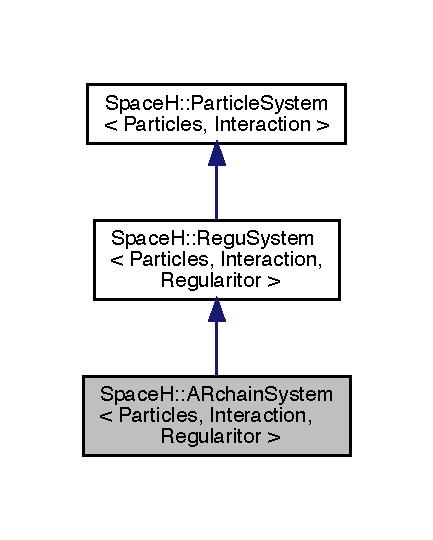
\includegraphics[width=208pt]{class_space_h_1_1_a_rchain_system__inherit__graph}
\end{center}
\end{figure}


Collaboration diagram for SpaceH\+:\+:A\+Rchain\+System$<$ Particles, Interaction, Regularitor $>$\+:
\nopagebreak
\begin{figure}[H]
\begin{center}
\leavevmode
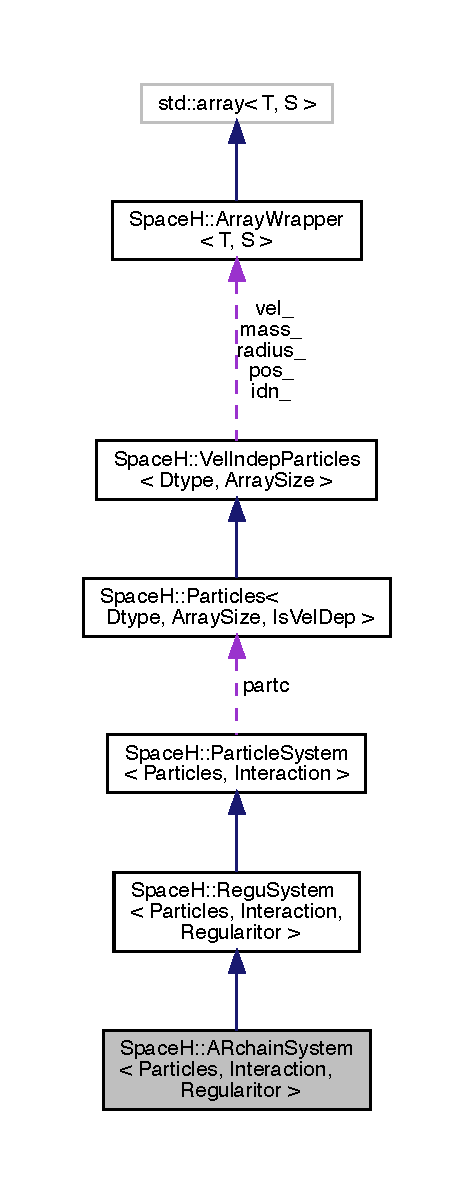
\includegraphics[height=550pt]{class_space_h_1_1_a_rchain_system__coll__graph}
\end{center}
\end{figure}
\subsection*{Public Types}
\begin{DoxyCompactItemize}
\item 
using \mbox{\hyperlink{class_space_h_1_1_a_rchain_system_a406ea4f9fd417879ac32c691bb705de4}{Base}} = \mbox{\hyperlink{class_space_h_1_1_regu_system}{Regu\+System}}$<$ \mbox{\hyperlink{struct_space_h_1_1_particles}{Particles}}, Interaction, Regularitor $>$
\item 
using \mbox{\hyperlink{class_space_h_1_1_a_rchain_system_a1830232bc4647fc2ef093696d76db007}{type}} = typename \mbox{\hyperlink{class_space_h_1_1_regu_system_a21376735739dfbe668a70cdba008baa3}{Base\+::type}}
\item 
using \mbox{\hyperlink{class_space_h_1_1_a_rchain_system_acaaa03940944dd5d6978c575888dd308}{Scalar}} = typename type\+::\+Scalar
\end{DoxyCompactItemize}
\subsection*{Public Member Functions}
\begin{DoxyCompactItemize}
\item 
void \mbox{\hyperlink{class_space_h_1_1_a_rchain_system_a2a0f231485f166cf9037a06a4b83e8ca}{after\+Iter\+Process}} ()
\item 
\mbox{\hyperlink{class_space_h_1_1_a_rchain_system_acaaa03940944dd5d6978c575888dd308}{Scalar}} \mbox{\hyperlink{class_space_h_1_1_a_rchain_system_adf6a2220ead064e01251a74ecbd7eb41}{potential\+Energy}} ()
\begin{DoxyCompactList}\small\item\em Calculate the potential energy of the system. \end{DoxyCompactList}\item 
\mbox{\hyperlink{class_space_h_1_1_a_rchain_system_acaaa03940944dd5d6978c575888dd308}{Scalar}} \mbox{\hyperlink{class_space_h_1_1_a_rchain_system_a069b5ae075413b26fa177df689bf044d}{total\+Energy}} ()
\begin{DoxyCompactList}\small\item\em Calculate the total energy of the system. \end{DoxyCompactList}\end{DoxyCompactItemize}
\subsection*{Additional Inherited Members}


\subsection{Detailed Description}
\subsubsection*{template$<$typename Particles, typename Interaction, typename Regularitor$>$\newline
class Space\+H\+::\+A\+Rchain\+System$<$ Particles, Interaction, Regularitor $>$}

Algorithmatic Regularization chain System. 

See details in \href{https://arxiv.org/abs/0709.3367}{\tt https\+://arxiv.\+org/abs/0709.\+3367} . 

\subsection{Member Typedef Documentation}
\mbox{\Hypertarget{class_space_h_1_1_a_rchain_system_a406ea4f9fd417879ac32c691bb705de4}\label{class_space_h_1_1_a_rchain_system_a406ea4f9fd417879ac32c691bb705de4}} 
\index{Space\+H\+::\+A\+Rchain\+System@{Space\+H\+::\+A\+Rchain\+System}!Base@{Base}}
\index{Base@{Base}!Space\+H\+::\+A\+Rchain\+System@{Space\+H\+::\+A\+Rchain\+System}}
\subsubsection{\texorpdfstring{Base}{Base}}
{\footnotesize\ttfamily template$<$typename Particles , typename Interaction , typename Regularitor $>$ \\
using \mbox{\hyperlink{class_space_h_1_1_a_rchain_system}{Space\+H\+::\+A\+Rchain\+System}}$<$ \mbox{\hyperlink{struct_space_h_1_1_particles}{Particles}}, Interaction, Regularitor $>$\+::\mbox{\hyperlink{class_space_h_1_1_a_rchain_system_a406ea4f9fd417879ac32c691bb705de4}{Base}} =  \mbox{\hyperlink{class_space_h_1_1_regu_system}{Regu\+System}}$<$\mbox{\hyperlink{struct_space_h_1_1_particles}{Particles}}, Interaction, Regularitor$>$}

\mbox{\Hypertarget{class_space_h_1_1_a_rchain_system_acaaa03940944dd5d6978c575888dd308}\label{class_space_h_1_1_a_rchain_system_acaaa03940944dd5d6978c575888dd308}} 
\index{Space\+H\+::\+A\+Rchain\+System@{Space\+H\+::\+A\+Rchain\+System}!Scalar@{Scalar}}
\index{Scalar@{Scalar}!Space\+H\+::\+A\+Rchain\+System@{Space\+H\+::\+A\+Rchain\+System}}
\subsubsection{\texorpdfstring{Scalar}{Scalar}}
{\footnotesize\ttfamily template$<$typename Particles , typename Interaction , typename Regularitor $>$ \\
using \mbox{\hyperlink{class_space_h_1_1_a_rchain_system}{Space\+H\+::\+A\+Rchain\+System}}$<$ \mbox{\hyperlink{struct_space_h_1_1_particles}{Particles}}, Interaction, Regularitor $>$\+::\mbox{\hyperlink{class_space_h_1_1_a_rchain_system_acaaa03940944dd5d6978c575888dd308}{Scalar}} =  typename type\+::\+Scalar}

\mbox{\Hypertarget{class_space_h_1_1_a_rchain_system_a1830232bc4647fc2ef093696d76db007}\label{class_space_h_1_1_a_rchain_system_a1830232bc4647fc2ef093696d76db007}} 
\index{Space\+H\+::\+A\+Rchain\+System@{Space\+H\+::\+A\+Rchain\+System}!type@{type}}
\index{type@{type}!Space\+H\+::\+A\+Rchain\+System@{Space\+H\+::\+A\+Rchain\+System}}
\subsubsection{\texorpdfstring{type}{type}}
{\footnotesize\ttfamily template$<$typename Particles , typename Interaction , typename Regularitor $>$ \\
using \mbox{\hyperlink{class_space_h_1_1_a_rchain_system}{Space\+H\+::\+A\+Rchain\+System}}$<$ \mbox{\hyperlink{struct_space_h_1_1_particles}{Particles}}, Interaction, Regularitor $>$\+::\mbox{\hyperlink{class_space_h_1_1_a_rchain_system_a1830232bc4647fc2ef093696d76db007}{type}} =  typename \mbox{\hyperlink{class_space_h_1_1_regu_system_a21376735739dfbe668a70cdba008baa3}{Base\+::type}}}



\subsection{Member Function Documentation}
\mbox{\Hypertarget{class_space_h_1_1_a_rchain_system_a2a0f231485f166cf9037a06a4b83e8ca}\label{class_space_h_1_1_a_rchain_system_a2a0f231485f166cf9037a06a4b83e8ca}} 
\index{Space\+H\+::\+A\+Rchain\+System@{Space\+H\+::\+A\+Rchain\+System}!after\+Iter\+Process@{after\+Iter\+Process}}
\index{after\+Iter\+Process@{after\+Iter\+Process}!Space\+H\+::\+A\+Rchain\+System@{Space\+H\+::\+A\+Rchain\+System}}
\subsubsection{\texorpdfstring{after\+Iter\+Process()}{afterIterProcess()}}
{\footnotesize\ttfamily template$<$typename Particles , typename Interaction , typename Regularitor $>$ \\
void \mbox{\hyperlink{class_space_h_1_1_a_rchain_system}{Space\+H\+::\+A\+Rchain\+System}}$<$ \mbox{\hyperlink{struct_space_h_1_1_particles}{Particles}}, Interaction, Regularitor $>$\+::after\+Iter\+Process (\begin{DoxyParamCaption}{ }\end{DoxyParamCaption})\hspace{0.3cm}{\ttfamily [inline]}}

Here is the call graph for this function\+:
\nopagebreak
\begin{figure}[H]
\begin{center}
\leavevmode
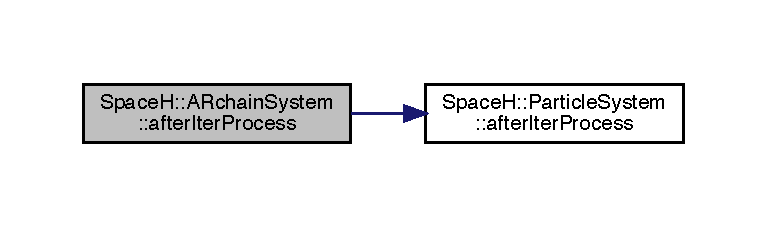
\includegraphics[width=350pt]{class_space_h_1_1_a_rchain_system_a2a0f231485f166cf9037a06a4b83e8ca_cgraph}
\end{center}
\end{figure}
\mbox{\Hypertarget{class_space_h_1_1_a_rchain_system_adf6a2220ead064e01251a74ecbd7eb41}\label{class_space_h_1_1_a_rchain_system_adf6a2220ead064e01251a74ecbd7eb41}} 
\index{Space\+H\+::\+A\+Rchain\+System@{Space\+H\+::\+A\+Rchain\+System}!potential\+Energy@{potential\+Energy}}
\index{potential\+Energy@{potential\+Energy}!Space\+H\+::\+A\+Rchain\+System@{Space\+H\+::\+A\+Rchain\+System}}
\subsubsection{\texorpdfstring{potential\+Energy()}{potentialEnergy()}}
{\footnotesize\ttfamily template$<$typename Particles , typename Interaction , typename Regularitor $>$ \\
\mbox{\hyperlink{class_space_h_1_1_a_rchain_system_acaaa03940944dd5d6978c575888dd308}{Scalar}} \mbox{\hyperlink{class_space_h_1_1_a_rchain_system}{Space\+H\+::\+A\+Rchain\+System}}$<$ \mbox{\hyperlink{struct_space_h_1_1_particles}{Particles}}, Interaction, Regularitor $>$\+::potential\+Energy (\begin{DoxyParamCaption}{ }\end{DoxyParamCaption})\hspace{0.3cm}{\ttfamily [inline]}}



Calculate the potential energy of the system. 

Here is the call graph for this function\+:
\nopagebreak
\begin{figure}[H]
\begin{center}
\leavevmode
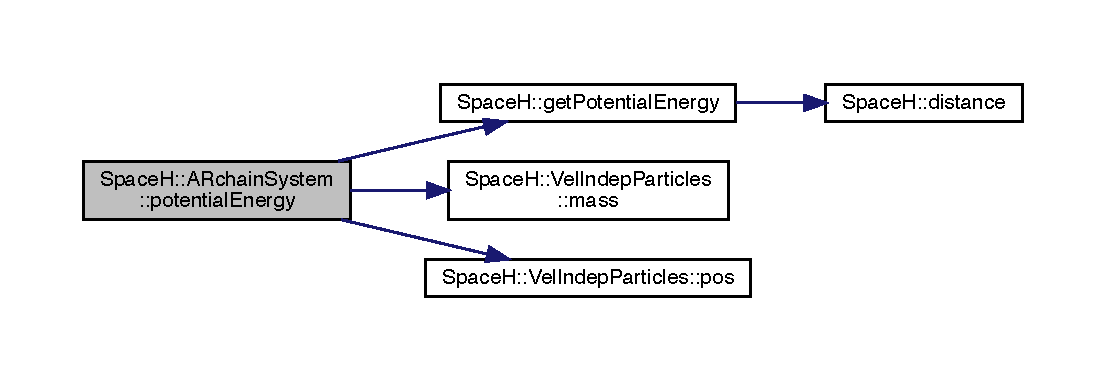
\includegraphics[width=350pt]{class_space_h_1_1_a_rchain_system_adf6a2220ead064e01251a74ecbd7eb41_cgraph}
\end{center}
\end{figure}
Here is the caller graph for this function\+:
\nopagebreak
\begin{figure}[H]
\begin{center}
\leavevmode
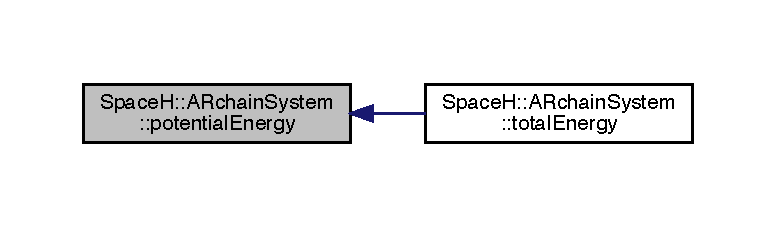
\includegraphics[width=350pt]{class_space_h_1_1_a_rchain_system_adf6a2220ead064e01251a74ecbd7eb41_icgraph}
\end{center}
\end{figure}
\mbox{\Hypertarget{class_space_h_1_1_a_rchain_system_a069b5ae075413b26fa177df689bf044d}\label{class_space_h_1_1_a_rchain_system_a069b5ae075413b26fa177df689bf044d}} 
\index{Space\+H\+::\+A\+Rchain\+System@{Space\+H\+::\+A\+Rchain\+System}!total\+Energy@{total\+Energy}}
\index{total\+Energy@{total\+Energy}!Space\+H\+::\+A\+Rchain\+System@{Space\+H\+::\+A\+Rchain\+System}}
\subsubsection{\texorpdfstring{total\+Energy()}{totalEnergy()}}
{\footnotesize\ttfamily template$<$typename Particles , typename Interaction , typename Regularitor $>$ \\
\mbox{\hyperlink{class_space_h_1_1_a_rchain_system_acaaa03940944dd5d6978c575888dd308}{Scalar}} \mbox{\hyperlink{class_space_h_1_1_a_rchain_system}{Space\+H\+::\+A\+Rchain\+System}}$<$ \mbox{\hyperlink{struct_space_h_1_1_particles}{Particles}}, Interaction, Regularitor $>$\+::total\+Energy (\begin{DoxyParamCaption}{ }\end{DoxyParamCaption})\hspace{0.3cm}{\ttfamily [inline]}}



Calculate the total energy of the system. 

Here is the call graph for this function\+:
\nopagebreak
\begin{figure}[H]
\begin{center}
\leavevmode
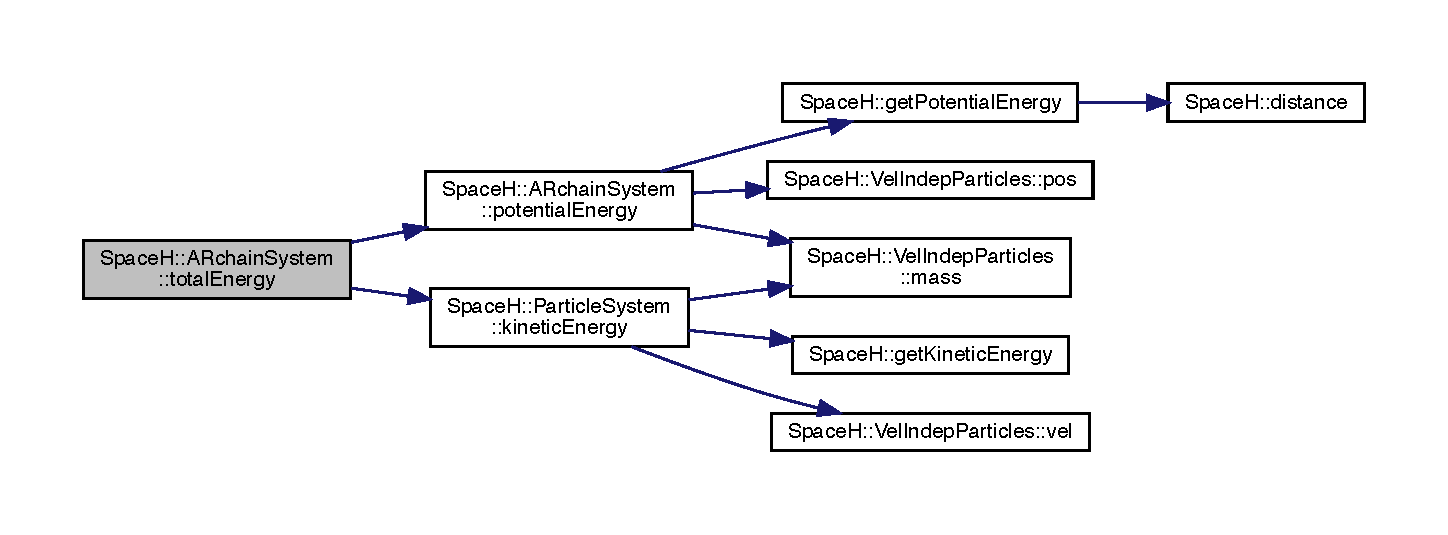
\includegraphics[width=350pt]{class_space_h_1_1_a_rchain_system_a069b5ae075413b26fa177df689bf044d_cgraph}
\end{center}
\end{figure}


The documentation for this class was generated from the following file\+:\begin{DoxyCompactItemize}
\item 
particle\+System/\+A\+R\+Chain/\mbox{\hyperlink{_a_rchain_system_8h}{A\+Rchain\+System.\+h}}\end{DoxyCompactItemize}

\hypertarget{struct_space_h_1_1_array_wrapper}{}\section{SpaceH\+:\+:Array\+Wrapper$<$ T, S $>$ Struct Template Reference}
\label{struct_space_h_1_1_array_wrapper}\index{Space\+H\+::\+Array\+Wrapper$<$ T, S $>$@{Space\+H\+::\+Array\+Wrapper$<$ T, S $>$}}


{\ttfamily \#include $<$proto\+Type.\+h$>$}



Inheritance diagram for SpaceH\+:\+:Array\+Wrapper$<$ T, S $>$\+:\nopagebreak
\begin{figure}[H]
\begin{center}
\leavevmode
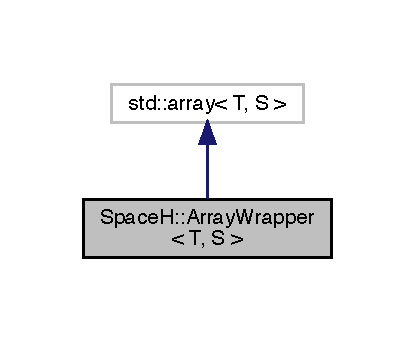
\includegraphics[width=199pt]{struct_space_h_1_1_array_wrapper__inherit__graph}
\end{center}
\end{figure}


Collaboration diagram for SpaceH\+:\+:Array\+Wrapper$<$ T, S $>$\+:\nopagebreak
\begin{figure}[H]
\begin{center}
\leavevmode
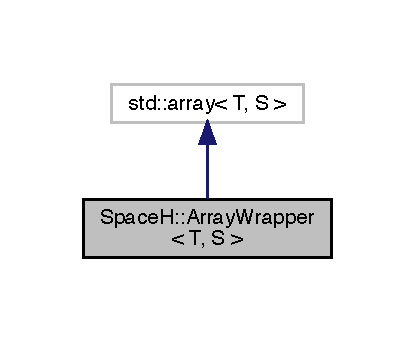
\includegraphics[width=199pt]{struct_space_h_1_1_array_wrapper__coll__graph}
\end{center}
\end{figure}
\subsection*{Public Member Functions}
\begin{DoxyCompactItemize}
\item 
void \mbox{\hyperlink{struct_space_h_1_1_array_wrapper_ac388a0420df96cf7fa128af10bd91514}{clear}} ()
\item 
void \mbox{\hyperlink{struct_space_h_1_1_array_wrapper_a0b6c9b3a863b31b77f67a61afdd3f6f1}{reserve}} (size\+\_\+t new\+\_\+cap)
\item 
void \mbox{\hyperlink{struct_space_h_1_1_array_wrapper_a5198ec13cd7200e87bd786bcc1692884}{resize}} (size\+\_\+t new\+\_\+size)
\end{DoxyCompactItemize}


\subsection{Member Function Documentation}
\mbox{\Hypertarget{struct_space_h_1_1_array_wrapper_ac388a0420df96cf7fa128af10bd91514}\label{struct_space_h_1_1_array_wrapper_ac388a0420df96cf7fa128af10bd91514}} 
\index{Space\+H\+::\+Array\+Wrapper@{Space\+H\+::\+Array\+Wrapper}!clear@{clear}}
\index{clear@{clear}!Space\+H\+::\+Array\+Wrapper@{Space\+H\+::\+Array\+Wrapper}}
\subsubsection{\texorpdfstring{clear()}{clear()}}
{\footnotesize\ttfamily template$<$typename T , size\+\_\+t S$>$ \\
void \mbox{\hyperlink{struct_space_h_1_1_array_wrapper}{Space\+H\+::\+Array\+Wrapper}}$<$ T, S $>$\+::clear (\begin{DoxyParamCaption}{ }\end{DoxyParamCaption})\hspace{0.3cm}{\ttfamily [inline]}}

\mbox{\Hypertarget{struct_space_h_1_1_array_wrapper_a0b6c9b3a863b31b77f67a61afdd3f6f1}\label{struct_space_h_1_1_array_wrapper_a0b6c9b3a863b31b77f67a61afdd3f6f1}} 
\index{Space\+H\+::\+Array\+Wrapper@{Space\+H\+::\+Array\+Wrapper}!reserve@{reserve}}
\index{reserve@{reserve}!Space\+H\+::\+Array\+Wrapper@{Space\+H\+::\+Array\+Wrapper}}
\subsubsection{\texorpdfstring{reserve()}{reserve()}}
{\footnotesize\ttfamily template$<$typename T , size\+\_\+t S$>$ \\
void \mbox{\hyperlink{struct_space_h_1_1_array_wrapper}{Space\+H\+::\+Array\+Wrapper}}$<$ T, S $>$\+::reserve (\begin{DoxyParamCaption}\item[{size\+\_\+t}]{new\+\_\+cap }\end{DoxyParamCaption})\hspace{0.3cm}{\ttfamily [inline]}}

\mbox{\Hypertarget{struct_space_h_1_1_array_wrapper_a5198ec13cd7200e87bd786bcc1692884}\label{struct_space_h_1_1_array_wrapper_a5198ec13cd7200e87bd786bcc1692884}} 
\index{Space\+H\+::\+Array\+Wrapper@{Space\+H\+::\+Array\+Wrapper}!resize@{resize}}
\index{resize@{resize}!Space\+H\+::\+Array\+Wrapper@{Space\+H\+::\+Array\+Wrapper}}
\subsubsection{\texorpdfstring{resize()}{resize()}}
{\footnotesize\ttfamily template$<$typename T , size\+\_\+t S$>$ \\
void \mbox{\hyperlink{struct_space_h_1_1_array_wrapper}{Space\+H\+::\+Array\+Wrapper}}$<$ T, S $>$\+::resize (\begin{DoxyParamCaption}\item[{size\+\_\+t}]{new\+\_\+size }\end{DoxyParamCaption})\hspace{0.3cm}{\ttfamily [inline]}}



The documentation for this struct was generated from the following file\+:\begin{DoxyCompactItemize}
\item 
\mbox{\hyperlink{proto_type_8h}{proto\+Type.\+h}}\end{DoxyCompactItemize}

\hypertarget{struct_space_h_1_1_array_wrapper_3_01_t_00_01_d_y_n_a_m_i_c_a_l_01_4}{}\section{SpaceH\+:\+:Array\+Wrapper$<$ T, D\+Y\+N\+A\+M\+I\+C\+AL $>$ Struct Template Reference}
\label{struct_space_h_1_1_array_wrapper_3_01_t_00_01_d_y_n_a_m_i_c_a_l_01_4}\index{Space\+H\+::\+Array\+Wrapper$<$ T, D\+Y\+N\+A\+M\+I\+C\+A\+L $>$@{Space\+H\+::\+Array\+Wrapper$<$ T, D\+Y\+N\+A\+M\+I\+C\+A\+L $>$}}


{\ttfamily \#include $<$proto\+Type.\+h$>$}



Inheritance diagram for SpaceH\+:\+:Array\+Wrapper$<$ T, D\+Y\+N\+A\+M\+I\+C\+AL $>$\+:\nopagebreak
\begin{figure}[H]
\begin{center}
\leavevmode
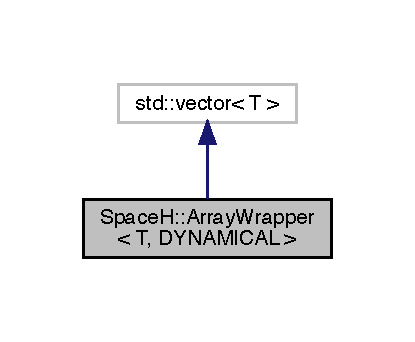
\includegraphics[width=199pt]{struct_space_h_1_1_array_wrapper_3_01_t_00_01_d_y_n_a_m_i_c_a_l_01_4__inherit__graph}
\end{center}
\end{figure}


Collaboration diagram for SpaceH\+:\+:Array\+Wrapper$<$ T, D\+Y\+N\+A\+M\+I\+C\+AL $>$\+:\nopagebreak
\begin{figure}[H]
\begin{center}
\leavevmode
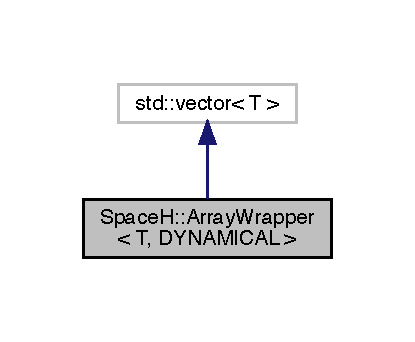
\includegraphics[width=199pt]{struct_space_h_1_1_array_wrapper_3_01_t_00_01_d_y_n_a_m_i_c_a_l_01_4__coll__graph}
\end{center}
\end{figure}


The documentation for this struct was generated from the following file\+:\begin{DoxyCompactItemize}
\item 
\mbox{\hyperlink{proto_type_8h}{proto\+Type.\+h}}\end{DoxyCompactItemize}

\hypertarget{struct_space_h_1_1big__value}{}\section{SpaceH\+:\+:big\+\_\+value$<$ Dtype $>$ Struct Template Reference}
\label{struct_space_h_1_1big__value}\index{Space\+H\+::big\+\_\+value$<$ Dtype $>$@{Space\+H\+::big\+\_\+value$<$ Dtype $>$}}


{\ttfamily \#include $<$own\+Math.\+h$>$}

\subsection*{Public Types}
\begin{DoxyCompactItemize}
\item 
using \mbox{\hyperlink{struct_space_h_1_1big__value_a8c1a5da25377f513b626b99b2c9e4e54}{value\+\_\+type}} = typename \mbox{\hyperlink{struct_space_h_1_1get__value__type}{Space\+H\+::get\+\_\+value\+\_\+type}}$<$ Dtype $>$\+::type
\end{DoxyCompactItemize}
\subsection*{Static Public Attributes}
\begin{DoxyCompactItemize}
\item 
static constexpr \mbox{\hyperlink{struct_space_h_1_1big__value_a8c1a5da25377f513b626b99b2c9e4e54}{value\+\_\+type}} \mbox{\hyperlink{struct_space_h_1_1big__value_a3191cef28acf20e7770b64e273802dda}{value}} = 0.\+1$\ast$std\+::numeric\+\_\+limits$<$\mbox{\hyperlink{struct_space_h_1_1big__value_a8c1a5da25377f513b626b99b2c9e4e54}{value\+\_\+type}}$>$\+::\mbox{\hyperlink{namespace_space_h_aacd80a06ba9a8b2381301a3917d79cbe}{max}}()
\end{DoxyCompactItemize}


\subsection{Member Typedef Documentation}
\mbox{\Hypertarget{struct_space_h_1_1big__value_a8c1a5da25377f513b626b99b2c9e4e54}\label{struct_space_h_1_1big__value_a8c1a5da25377f513b626b99b2c9e4e54}} 
\index{Space\+H\+::big\+\_\+value@{Space\+H\+::big\+\_\+value}!value\+\_\+type@{value\+\_\+type}}
\index{value\+\_\+type@{value\+\_\+type}!Space\+H\+::big\+\_\+value@{Space\+H\+::big\+\_\+value}}
\subsubsection{\texorpdfstring{value\+\_\+type}{value\_type}}
{\footnotesize\ttfamily template$<$typename Dtype $>$ \\
using \mbox{\hyperlink{struct_space_h_1_1big__value}{Space\+H\+::big\+\_\+value}}$<$ Dtype $>$\+::\mbox{\hyperlink{struct_space_h_1_1big__value_a8c1a5da25377f513b626b99b2c9e4e54}{value\+\_\+type}} =  typename \mbox{\hyperlink{struct_space_h_1_1get__value__type}{Space\+H\+::get\+\_\+value\+\_\+type}}$<$Dtype$>$\+::type}



\subsection{Member Data Documentation}
\mbox{\Hypertarget{struct_space_h_1_1big__value_a3191cef28acf20e7770b64e273802dda}\label{struct_space_h_1_1big__value_a3191cef28acf20e7770b64e273802dda}} 
\index{Space\+H\+::big\+\_\+value@{Space\+H\+::big\+\_\+value}!value@{value}}
\index{value@{value}!Space\+H\+::big\+\_\+value@{Space\+H\+::big\+\_\+value}}
\subsubsection{\texorpdfstring{value}{value}}
{\footnotesize\ttfamily template$<$typename Dtype $>$ \\
constexpr \mbox{\hyperlink{struct_space_h_1_1big__value_a8c1a5da25377f513b626b99b2c9e4e54}{value\+\_\+type}} \mbox{\hyperlink{struct_space_h_1_1big__value}{Space\+H\+::big\+\_\+value}}$<$ Dtype $>$\+::value = 0.\+1$\ast$std\+::numeric\+\_\+limits$<$\mbox{\hyperlink{struct_space_h_1_1big__value_a8c1a5da25377f513b626b99b2c9e4e54}{value\+\_\+type}}$>$\+::\mbox{\hyperlink{namespace_space_h_aacd80a06ba9a8b2381301a3917d79cbe}{max}}()\hspace{0.3cm}{\ttfamily [static]}}



The documentation for this struct was generated from the following file\+:\begin{DoxyCompactItemize}
\item 
\mbox{\hyperlink{own_math_8h}{own\+Math.\+h}}\end{DoxyCompactItemize}

\hypertarget{class_space_h_1_1_b_s_iterator}{}\section{SpaceH\+:\+:B\+S\+Iterator$<$ Partic\+Sys, Integrator $>$ Class Template Reference}
\label{class_space_h_1_1_b_s_iterator}\index{Space\+H\+::\+B\+S\+Iterator$<$ Partic\+Sys, Integrator $>$@{Space\+H\+::\+B\+S\+Iterator$<$ Partic\+Sys, Integrator $>$}}


Bulirsch-\/\+Stoer extrapolation algorithm.  




{\ttfamily \#include $<$B\+S\+Iterator.\+h$>$}

\subsection*{Public Types}
\begin{DoxyCompactItemize}
\item 
using \mbox{\hyperlink{class_space_h_1_1_b_s_iterator_a659e97efd0fe41f3993663d0ec9b75e7}{type}} = typename Partic\+Sys\+::type
\item 
using \mbox{\hyperlink{class_space_h_1_1_b_s_iterator_a89993409583b3022709bdfd84ea8149d}{Scalar}} = typename type\+::\+Scalar
\item 
using \mbox{\hyperlink{class_space_h_1_1_b_s_iterator_a3c3609d40e0ac4268760adeb1f0514de}{Scalar\+Buffer}} = typename type\+::\+Scalar\+Buffer
\item 
{\footnotesize template$<$typename T , size\+\_\+t S$>$ }\\using \mbox{\hyperlink{class_space_h_1_1_b_s_iterator_a6f704f5db07202710306e6e334c99e2f}{Container}} = typename type\+::template \mbox{\hyperlink{class_space_h_1_1_b_s_iterator_a6f704f5db07202710306e6e334c99e2f}{Container}}$<$ T, S $>$
\item 
using \mbox{\hyperlink{class_space_h_1_1_b_s_iterator_a659e97efd0fe41f3993663d0ec9b75e7}{type}} = typename Partic\+Sys\+::type
\item 
using \mbox{\hyperlink{class_space_h_1_1_b_s_iterator_a89993409583b3022709bdfd84ea8149d}{Scalar}} = typename type\+::\+Scalar
\item 
using \mbox{\hyperlink{class_space_h_1_1_b_s_iterator_a3c3609d40e0ac4268760adeb1f0514de}{Scalar\+Buffer}} = typename type\+::\+Scalar\+Buffer
\item 
{\footnotesize template$<$typename T , size\+\_\+t S$>$ }\\using \mbox{\hyperlink{class_space_h_1_1_b_s_iterator_a6f704f5db07202710306e6e334c99e2f}{Container}} = typename type\+::template \mbox{\hyperlink{class_space_h_1_1_b_s_iterator_a6f704f5db07202710306e6e334c99e2f}{Container}}$<$ T, S $>$
\end{DoxyCompactItemize}
\subsection*{Public Member Functions}
\begin{DoxyCompactItemize}
\item 
\mbox{\hyperlink{class_space_h_1_1_b_s_iterator_aef64ddf4540fa44e7c408e0ed7caabb2}{B\+S\+Iterator}} ()
\begin{DoxyCompactList}\small\item\em Constructor for initializing work\+\_\+, n\+Steps, fmin and CC. \end{DoxyCompactList}\item 
\mbox{\hyperlink{class_space_h_1_1_b_s_iterator_a89993409583b3022709bdfd84ea8149d}{Scalar}} \mbox{\hyperlink{class_space_h_1_1_b_s_iterator_a5ddc9dbcdecb554d58952c3b002e6b5e}{iterate}} (Partic\+Sys \&particles, \mbox{\hyperlink{class_space_h_1_1_b_s_iterator_a89993409583b3022709bdfd84ea8149d}{Scalar}} step\+Length)
\begin{DoxyCompactList}\small\item\em Interface of O\+DE iterator. \end{DoxyCompactList}\item 
void \mbox{\hyperlink{class_space_h_1_1_b_s_iterator_a8ac161c12bba12277bb9c881b692f60a}{set\+Relative\+Error}} (\mbox{\hyperlink{class_space_h_1_1_b_s_iterator_a89993409583b3022709bdfd84ea8149d}{Scalar}} rel\+Error)
\begin{DoxyCompactList}\small\item\em Set the local relative error. \end{DoxyCompactList}\item 
\mbox{\hyperlink{class_space_h_1_1_b_s_iterator_a89993409583b3022709bdfd84ea8149d}{Scalar}} \mbox{\hyperlink{class_space_h_1_1_b_s_iterator_a86345cb32e6cb2da0437a3697866501f}{get\+Rej\+Rate}} ()
\item 
\mbox{\hyperlink{class_space_h_1_1_b_s_iterator_aef64ddf4540fa44e7c408e0ed7caabb2}{B\+S\+Iterator}} ()
\begin{DoxyCompactList}\small\item\em Constructor for initializing cost, n\+Steps, fmin and CC. \end{DoxyCompactList}\item 
\mbox{\hyperlink{class_space_h_1_1_b_s_iterator_a89993409583b3022709bdfd84ea8149d}{Scalar}} \mbox{\hyperlink{class_space_h_1_1_b_s_iterator_afd196cc621849edd195622dfb5f83719}{iterate}} (Partic\+Sys \&particles, \mbox{\hyperlink{class_space_h_1_1_b_s_iterator_a89993409583b3022709bdfd84ea8149d}{Scalar}} step\+Length)
\begin{DoxyCompactList}\small\item\em Interface of O\+DE iterator. \end{DoxyCompactList}\item 
void \mbox{\hyperlink{class_space_h_1_1_b_s_iterator_a8ac161c12bba12277bb9c881b692f60a}{set\+Relative\+Error}} (\mbox{\hyperlink{class_space_h_1_1_b_s_iterator_a89993409583b3022709bdfd84ea8149d}{Scalar}} rel\+Error)
\begin{DoxyCompactList}\small\item\em Set the local relative error. \end{DoxyCompactList}\item 
void \mbox{\hyperlink{class_space_h_1_1_b_s_iterator_a632afee18728553ba785f7b9468833e7}{set\+Absolute\+Error}} (\mbox{\hyperlink{class_space_h_1_1_b_s_iterator_a89993409583b3022709bdfd84ea8149d}{Scalar}} abs\+Error)
\begin{DoxyCompactList}\small\item\em Set the local absolute error. \end{DoxyCompactList}\item 
\mbox{\hyperlink{class_space_h_1_1_b_s_iterator_a89993409583b3022709bdfd84ea8149d}{Scalar}} \mbox{\hyperlink{class_space_h_1_1_b_s_iterator_a86345cb32e6cb2da0437a3697866501f}{get\+Rej\+Rate}} ()
\item 
\mbox{\hyperlink{class_space_h_1_1_b_s_iterator_a89993409583b3022709bdfd84ea8149d}{Scalar}} \mbox{\hyperlink{class_space_h_1_1_b_s_iterator_aac17462f691d6e8c1adee5d14f066e75}{get\+Efficiency}} ()
\end{DoxyCompactItemize}


\subsection{Detailed Description}
\subsubsection*{template$<$typename Partic\+Sys, typename Integrator$>$\newline
class Space\+H\+::\+B\+S\+Iterator$<$ Partic\+Sys, Integrator $>$}

Bulirsch-\/\+Stoer extrapolation algorithm. 

\subsection{Member Typedef Documentation}
\mbox{\Hypertarget{class_space_h_1_1_b_s_iterator_a6f704f5db07202710306e6e334c99e2f}\label{class_space_h_1_1_b_s_iterator_a6f704f5db07202710306e6e334c99e2f}} 
\index{Space\+H\+::\+B\+S\+Iterator@{Space\+H\+::\+B\+S\+Iterator}!Container@{Container}}
\index{Container@{Container}!Space\+H\+::\+B\+S\+Iterator@{Space\+H\+::\+B\+S\+Iterator}}
\subsubsection{\texorpdfstring{Container}{Container}\hspace{0.1cm}{\footnotesize\ttfamily [1/2]}}
{\footnotesize\ttfamily template$<$typename Partic\+Sys , typename Integrator $>$ \\
template$<$typename T , size\+\_\+t S$>$ \\
using \mbox{\hyperlink{class_space_h_1_1_b_s_iterator}{Space\+H\+::\+B\+S\+Iterator}}$<$ Partic\+Sys, Integrator $>$\+::\mbox{\hyperlink{class_space_h_1_1_b_s_iterator_a6f704f5db07202710306e6e334c99e2f}{Container}} =  typename type\+::template \mbox{\hyperlink{class_space_h_1_1_b_s_iterator_a6f704f5db07202710306e6e334c99e2f}{Container}}$<$T, S$>$}

\mbox{\Hypertarget{class_space_h_1_1_b_s_iterator_a6f704f5db07202710306e6e334c99e2f}\label{class_space_h_1_1_b_s_iterator_a6f704f5db07202710306e6e334c99e2f}} 
\index{Space\+H\+::\+B\+S\+Iterator@{Space\+H\+::\+B\+S\+Iterator}!Container@{Container}}
\index{Container@{Container}!Space\+H\+::\+B\+S\+Iterator@{Space\+H\+::\+B\+S\+Iterator}}
\subsubsection{\texorpdfstring{Container}{Container}\hspace{0.1cm}{\footnotesize\ttfamily [2/2]}}
{\footnotesize\ttfamily template$<$typename Partic\+Sys , typename Integrator $>$ \\
template$<$typename T , size\+\_\+t S$>$ \\
using \mbox{\hyperlink{class_space_h_1_1_b_s_iterator}{Space\+H\+::\+B\+S\+Iterator}}$<$ Partic\+Sys, Integrator $>$\+::\mbox{\hyperlink{class_space_h_1_1_b_s_iterator_a6f704f5db07202710306e6e334c99e2f}{Container}} =  typename type\+::template \mbox{\hyperlink{class_space_h_1_1_b_s_iterator_a6f704f5db07202710306e6e334c99e2f}{Container}}$<$T, S$>$}

\mbox{\Hypertarget{class_space_h_1_1_b_s_iterator_a89993409583b3022709bdfd84ea8149d}\label{class_space_h_1_1_b_s_iterator_a89993409583b3022709bdfd84ea8149d}} 
\index{Space\+H\+::\+B\+S\+Iterator@{Space\+H\+::\+B\+S\+Iterator}!Scalar@{Scalar}}
\index{Scalar@{Scalar}!Space\+H\+::\+B\+S\+Iterator@{Space\+H\+::\+B\+S\+Iterator}}
\subsubsection{\texorpdfstring{Scalar}{Scalar}\hspace{0.1cm}{\footnotesize\ttfamily [1/2]}}
{\footnotesize\ttfamily template$<$typename Partic\+Sys , typename Integrator $>$ \\
using \mbox{\hyperlink{class_space_h_1_1_b_s_iterator}{Space\+H\+::\+B\+S\+Iterator}}$<$ Partic\+Sys, Integrator $>$\+::\mbox{\hyperlink{class_space_h_1_1_b_s_iterator_a89993409583b3022709bdfd84ea8149d}{Scalar}} =  typename type\+::\+Scalar}

\mbox{\Hypertarget{class_space_h_1_1_b_s_iterator_a89993409583b3022709bdfd84ea8149d}\label{class_space_h_1_1_b_s_iterator_a89993409583b3022709bdfd84ea8149d}} 
\index{Space\+H\+::\+B\+S\+Iterator@{Space\+H\+::\+B\+S\+Iterator}!Scalar@{Scalar}}
\index{Scalar@{Scalar}!Space\+H\+::\+B\+S\+Iterator@{Space\+H\+::\+B\+S\+Iterator}}
\subsubsection{\texorpdfstring{Scalar}{Scalar}\hspace{0.1cm}{\footnotesize\ttfamily [2/2]}}
{\footnotesize\ttfamily template$<$typename Partic\+Sys , typename Integrator $>$ \\
using \mbox{\hyperlink{class_space_h_1_1_b_s_iterator}{Space\+H\+::\+B\+S\+Iterator}}$<$ Partic\+Sys, Integrator $>$\+::\mbox{\hyperlink{class_space_h_1_1_b_s_iterator_a89993409583b3022709bdfd84ea8149d}{Scalar}} =  typename type\+::\+Scalar}

\mbox{\Hypertarget{class_space_h_1_1_b_s_iterator_a3c3609d40e0ac4268760adeb1f0514de}\label{class_space_h_1_1_b_s_iterator_a3c3609d40e0ac4268760adeb1f0514de}} 
\index{Space\+H\+::\+B\+S\+Iterator@{Space\+H\+::\+B\+S\+Iterator}!Scalar\+Buffer@{Scalar\+Buffer}}
\index{Scalar\+Buffer@{Scalar\+Buffer}!Space\+H\+::\+B\+S\+Iterator@{Space\+H\+::\+B\+S\+Iterator}}
\subsubsection{\texorpdfstring{Scalar\+Buffer}{ScalarBuffer}\hspace{0.1cm}{\footnotesize\ttfamily [1/2]}}
{\footnotesize\ttfamily template$<$typename Partic\+Sys , typename Integrator $>$ \\
using \mbox{\hyperlink{class_space_h_1_1_b_s_iterator}{Space\+H\+::\+B\+S\+Iterator}}$<$ Partic\+Sys, Integrator $>$\+::\mbox{\hyperlink{class_space_h_1_1_b_s_iterator_a3c3609d40e0ac4268760adeb1f0514de}{Scalar\+Buffer}} =  typename type\+::\+Scalar\+Buffer}

\mbox{\Hypertarget{class_space_h_1_1_b_s_iterator_a3c3609d40e0ac4268760adeb1f0514de}\label{class_space_h_1_1_b_s_iterator_a3c3609d40e0ac4268760adeb1f0514de}} 
\index{Space\+H\+::\+B\+S\+Iterator@{Space\+H\+::\+B\+S\+Iterator}!Scalar\+Buffer@{Scalar\+Buffer}}
\index{Scalar\+Buffer@{Scalar\+Buffer}!Space\+H\+::\+B\+S\+Iterator@{Space\+H\+::\+B\+S\+Iterator}}
\subsubsection{\texorpdfstring{Scalar\+Buffer}{ScalarBuffer}\hspace{0.1cm}{\footnotesize\ttfamily [2/2]}}
{\footnotesize\ttfamily template$<$typename Partic\+Sys , typename Integrator $>$ \\
using \mbox{\hyperlink{class_space_h_1_1_b_s_iterator}{Space\+H\+::\+B\+S\+Iterator}}$<$ Partic\+Sys, Integrator $>$\+::\mbox{\hyperlink{class_space_h_1_1_b_s_iterator_a3c3609d40e0ac4268760adeb1f0514de}{Scalar\+Buffer}} =  typename type\+::\+Scalar\+Buffer}

\mbox{\Hypertarget{class_space_h_1_1_b_s_iterator_a659e97efd0fe41f3993663d0ec9b75e7}\label{class_space_h_1_1_b_s_iterator_a659e97efd0fe41f3993663d0ec9b75e7}} 
\index{Space\+H\+::\+B\+S\+Iterator@{Space\+H\+::\+B\+S\+Iterator}!type@{type}}
\index{type@{type}!Space\+H\+::\+B\+S\+Iterator@{Space\+H\+::\+B\+S\+Iterator}}
\subsubsection{\texorpdfstring{type}{type}\hspace{0.1cm}{\footnotesize\ttfamily [1/2]}}
{\footnotesize\ttfamily template$<$typename Partic\+Sys , typename Integrator $>$ \\
using \mbox{\hyperlink{class_space_h_1_1_b_s_iterator}{Space\+H\+::\+B\+S\+Iterator}}$<$ Partic\+Sys, Integrator $>$\+::\mbox{\hyperlink{class_space_h_1_1_b_s_iterator_a659e97efd0fe41f3993663d0ec9b75e7}{type}} =  typename Partic\+Sys\+::type}

\mbox{\Hypertarget{class_space_h_1_1_b_s_iterator_a659e97efd0fe41f3993663d0ec9b75e7}\label{class_space_h_1_1_b_s_iterator_a659e97efd0fe41f3993663d0ec9b75e7}} 
\index{Space\+H\+::\+B\+S\+Iterator@{Space\+H\+::\+B\+S\+Iterator}!type@{type}}
\index{type@{type}!Space\+H\+::\+B\+S\+Iterator@{Space\+H\+::\+B\+S\+Iterator}}
\subsubsection{\texorpdfstring{type}{type}\hspace{0.1cm}{\footnotesize\ttfamily [2/2]}}
{\footnotesize\ttfamily template$<$typename Partic\+Sys , typename Integrator $>$ \\
using \mbox{\hyperlink{class_space_h_1_1_b_s_iterator}{Space\+H\+::\+B\+S\+Iterator}}$<$ Partic\+Sys, Integrator $>$\+::\mbox{\hyperlink{class_space_h_1_1_b_s_iterator_a659e97efd0fe41f3993663d0ec9b75e7}{type}} =  typename Partic\+Sys\+::type}



\subsection{Constructor \& Destructor Documentation}
\mbox{\Hypertarget{class_space_h_1_1_b_s_iterator_aef64ddf4540fa44e7c408e0ed7caabb2}\label{class_space_h_1_1_b_s_iterator_aef64ddf4540fa44e7c408e0ed7caabb2}} 
\index{Space\+H\+::\+B\+S\+Iterator@{Space\+H\+::\+B\+S\+Iterator}!B\+S\+Iterator@{B\+S\+Iterator}}
\index{B\+S\+Iterator@{B\+S\+Iterator}!Space\+H\+::\+B\+S\+Iterator@{Space\+H\+::\+B\+S\+Iterator}}
\subsubsection{\texorpdfstring{B\+S\+Iterator()}{BSIterator()}\hspace{0.1cm}{\footnotesize\ttfamily [1/2]}}
{\footnotesize\ttfamily template$<$typename Partic\+Sys , typename Integrator $>$ \\
\mbox{\hyperlink{class_space_h_1_1_b_s_iterator}{Space\+H\+::\+B\+S\+Iterator}}$<$ Partic\+Sys, Integrator $>$\+::\mbox{\hyperlink{class_space_h_1_1_b_s_iterator}{B\+S\+Iterator}} (\begin{DoxyParamCaption}{ }\end{DoxyParamCaption})}



Constructor for initializing work\+\_\+, n\+Steps, fmin and CC. 

Constructor for initializing cost, n\+Steps, fmin and CC. \mbox{\Hypertarget{class_space_h_1_1_b_s_iterator_aef64ddf4540fa44e7c408e0ed7caabb2}\label{class_space_h_1_1_b_s_iterator_aef64ddf4540fa44e7c408e0ed7caabb2}} 
\index{Space\+H\+::\+B\+S\+Iterator@{Space\+H\+::\+B\+S\+Iterator}!B\+S\+Iterator@{B\+S\+Iterator}}
\index{B\+S\+Iterator@{B\+S\+Iterator}!Space\+H\+::\+B\+S\+Iterator@{Space\+H\+::\+B\+S\+Iterator}}
\subsubsection{\texorpdfstring{B\+S\+Iterator()}{BSIterator()}\hspace{0.1cm}{\footnotesize\ttfamily [2/2]}}
{\footnotesize\ttfamily template$<$typename Partic\+Sys , typename Integrator $>$ \\
\mbox{\hyperlink{class_space_h_1_1_b_s_iterator}{Space\+H\+::\+B\+S\+Iterator}}$<$ Partic\+Sys, Integrator $>$\+::\mbox{\hyperlink{class_space_h_1_1_b_s_iterator}{B\+S\+Iterator}} (\begin{DoxyParamCaption}{ }\end{DoxyParamCaption})}



Constructor for initializing cost, n\+Steps, fmin and CC. 



\subsection{Member Function Documentation}
\mbox{\Hypertarget{class_space_h_1_1_b_s_iterator_aac17462f691d6e8c1adee5d14f066e75}\label{class_space_h_1_1_b_s_iterator_aac17462f691d6e8c1adee5d14f066e75}} 
\index{Space\+H\+::\+B\+S\+Iterator@{Space\+H\+::\+B\+S\+Iterator}!get\+Efficiency@{get\+Efficiency}}
\index{get\+Efficiency@{get\+Efficiency}!Space\+H\+::\+B\+S\+Iterator@{Space\+H\+::\+B\+S\+Iterator}}
\subsubsection{\texorpdfstring{get\+Efficiency()}{getEfficiency()}}
{\footnotesize\ttfamily template$<$typename Partic\+Sys , typename Integrator $>$ \\
\mbox{\hyperlink{class_space_h_1_1_b_s_iterator_a89993409583b3022709bdfd84ea8149d}{Scalar}} \mbox{\hyperlink{class_space_h_1_1_b_s_iterator}{Space\+H\+::\+B\+S\+Iterator}}$<$ Partic\+Sys, Integrator $>$\+::get\+Efficiency (\begin{DoxyParamCaption}{ }\end{DoxyParamCaption})\hspace{0.3cm}{\ttfamily [inline]}}

\mbox{\Hypertarget{class_space_h_1_1_b_s_iterator_a86345cb32e6cb2da0437a3697866501f}\label{class_space_h_1_1_b_s_iterator_a86345cb32e6cb2da0437a3697866501f}} 
\index{Space\+H\+::\+B\+S\+Iterator@{Space\+H\+::\+B\+S\+Iterator}!get\+Rej\+Rate@{get\+Rej\+Rate}}
\index{get\+Rej\+Rate@{get\+Rej\+Rate}!Space\+H\+::\+B\+S\+Iterator@{Space\+H\+::\+B\+S\+Iterator}}
\subsubsection{\texorpdfstring{get\+Rej\+Rate()}{getRejRate()}\hspace{0.1cm}{\footnotesize\ttfamily [1/2]}}
{\footnotesize\ttfamily template$<$typename Partic\+Sys , typename Integrator $>$ \\
\mbox{\hyperlink{class_space_h_1_1_b_s_iterator_a89993409583b3022709bdfd84ea8149d}{Scalar}} \mbox{\hyperlink{class_space_h_1_1_b_s_iterator}{Space\+H\+::\+B\+S\+Iterator}}$<$ Partic\+Sys, Integrator $>$\+::get\+Rej\+Rate (\begin{DoxyParamCaption}{ }\end{DoxyParamCaption})\hspace{0.3cm}{\ttfamily [inline]}}

\mbox{\Hypertarget{class_space_h_1_1_b_s_iterator_a86345cb32e6cb2da0437a3697866501f}\label{class_space_h_1_1_b_s_iterator_a86345cb32e6cb2da0437a3697866501f}} 
\index{Space\+H\+::\+B\+S\+Iterator@{Space\+H\+::\+B\+S\+Iterator}!get\+Rej\+Rate@{get\+Rej\+Rate}}
\index{get\+Rej\+Rate@{get\+Rej\+Rate}!Space\+H\+::\+B\+S\+Iterator@{Space\+H\+::\+B\+S\+Iterator}}
\subsubsection{\texorpdfstring{get\+Rej\+Rate()}{getRejRate()}\hspace{0.1cm}{\footnotesize\ttfamily [2/2]}}
{\footnotesize\ttfamily template$<$typename Partic\+Sys , typename Integrator $>$ \\
\mbox{\hyperlink{class_space_h_1_1_b_s_iterator_a89993409583b3022709bdfd84ea8149d}{Scalar}} \mbox{\hyperlink{class_space_h_1_1_b_s_iterator}{Space\+H\+::\+B\+S\+Iterator}}$<$ Partic\+Sys, Integrator $>$\+::get\+Rej\+Rate (\begin{DoxyParamCaption}{ }\end{DoxyParamCaption})\hspace{0.3cm}{\ttfamily [inline]}}

\mbox{\Hypertarget{class_space_h_1_1_b_s_iterator_afd196cc621849edd195622dfb5f83719}\label{class_space_h_1_1_b_s_iterator_afd196cc621849edd195622dfb5f83719}} 
\index{Space\+H\+::\+B\+S\+Iterator@{Space\+H\+::\+B\+S\+Iterator}!iterate@{iterate}}
\index{iterate@{iterate}!Space\+H\+::\+B\+S\+Iterator@{Space\+H\+::\+B\+S\+Iterator}}
\subsubsection{\texorpdfstring{iterate()}{iterate()}\hspace{0.1cm}{\footnotesize\ttfamily [1/2]}}
{\footnotesize\ttfamily template$<$typename Partic\+Sys , typename Integrator $>$ \\
\mbox{\hyperlink{class_space_h_1_1_b_s_iterator_a89993409583b3022709bdfd84ea8149d}{Scalar}} \mbox{\hyperlink{class_space_h_1_1_b_s_iterator}{Space\+H\+::\+B\+S\+Iterator}}$<$ Partic\+Sys, Integrator $>$\+::iterate (\begin{DoxyParamCaption}\item[{Partic\+Sys \&}]{particles,  }\item[{\mbox{\hyperlink{class_space_h_1_1_b_s_iterator_a89993409583b3022709bdfd84ea8149d}{Scalar}}}]{step\+Length }\end{DoxyParamCaption})}



Interface of O\+DE iterator. 

\begin{DoxyNote}{Note}
B\+Siterator will force use the internal mid-\/point integrator as the basic integrator. 
\end{DoxyNote}
\mbox{\Hypertarget{class_space_h_1_1_b_s_iterator_a5ddc9dbcdecb554d58952c3b002e6b5e}\label{class_space_h_1_1_b_s_iterator_a5ddc9dbcdecb554d58952c3b002e6b5e}} 
\index{Space\+H\+::\+B\+S\+Iterator@{Space\+H\+::\+B\+S\+Iterator}!iterate@{iterate}}
\index{iterate@{iterate}!Space\+H\+::\+B\+S\+Iterator@{Space\+H\+::\+B\+S\+Iterator}}
\subsubsection{\texorpdfstring{iterate()}{iterate()}\hspace{0.1cm}{\footnotesize\ttfamily [2/2]}}
{\footnotesize\ttfamily template$<$typename Partic\+Sys , typename Integrator $>$ \\
\mbox{\hyperlink{test_orbit_8cpp_a8c2981f3f834be9448a6ab06c28748eb}{Partic\+Sys\+::type\+::\+Scalar}} \mbox{\hyperlink{class_space_h_1_1_b_s_iterator}{Space\+H\+::\+B\+S\+Iterator}}$<$ Partic\+Sys, Integrator $>$\+::iterate (\begin{DoxyParamCaption}\item[{Partic\+Sys \&}]{particles,  }\item[{\mbox{\hyperlink{class_space_h_1_1_b_s_iterator_a89993409583b3022709bdfd84ea8149d}{Scalar}}}]{step\+Length }\end{DoxyParamCaption})}



Interface of O\+DE iterator. 

\begin{DoxyNote}{Note}
B\+Siterator will force use the internal mid-\/point integrator as the basic integrator.
\end{DoxyNote}

\begin{DoxyParams}{Parameters}
{\em particles} & \mbox{\hyperlink{struct_space_h_1_1_particle}{Particle}} system need iteration. \\
\hline
{\em integrator} & Basica integrator used to evolve, but here BS iterator will force use internal mid-\/point integrator. \\
\hline
{\em step\+Length} & Macro integration step length. \\
\hline
\end{DoxyParams}
\begin{DoxyReturn}{Returns}
The next macro integration step length. 
\end{DoxyReturn}
\mbox{\Hypertarget{class_space_h_1_1_b_s_iterator_a632afee18728553ba785f7b9468833e7}\label{class_space_h_1_1_b_s_iterator_a632afee18728553ba785f7b9468833e7}} 
\index{Space\+H\+::\+B\+S\+Iterator@{Space\+H\+::\+B\+S\+Iterator}!set\+Absolute\+Error@{set\+Absolute\+Error}}
\index{set\+Absolute\+Error@{set\+Absolute\+Error}!Space\+H\+::\+B\+S\+Iterator@{Space\+H\+::\+B\+S\+Iterator}}
\subsubsection{\texorpdfstring{set\+Absolute\+Error()}{setAbsoluteError()}}
{\footnotesize\ttfamily template$<$typename Partic\+Sys , typename Integrator $>$ \\
void \mbox{\hyperlink{class_space_h_1_1_b_s_iterator}{Space\+H\+::\+B\+S\+Iterator}}$<$ Partic\+Sys, Integrator $>$\+::set\+Absolute\+Error (\begin{DoxyParamCaption}\item[{\mbox{\hyperlink{class_space_h_1_1_b_s_iterator_a89993409583b3022709bdfd84ea8149d}{Scalar}}}]{abs\+Error }\end{DoxyParamCaption})\hspace{0.3cm}{\ttfamily [inline]}}



Set the local absolute error. 

\mbox{\Hypertarget{class_space_h_1_1_b_s_iterator_a8ac161c12bba12277bb9c881b692f60a}\label{class_space_h_1_1_b_s_iterator_a8ac161c12bba12277bb9c881b692f60a}} 
\index{Space\+H\+::\+B\+S\+Iterator@{Space\+H\+::\+B\+S\+Iterator}!set\+Relative\+Error@{set\+Relative\+Error}}
\index{set\+Relative\+Error@{set\+Relative\+Error}!Space\+H\+::\+B\+S\+Iterator@{Space\+H\+::\+B\+S\+Iterator}}
\subsubsection{\texorpdfstring{set\+Relative\+Error()}{setRelativeError()}\hspace{0.1cm}{\footnotesize\ttfamily [1/2]}}
{\footnotesize\ttfamily template$<$typename Partic\+Sys , typename Integrator $>$ \\
void \mbox{\hyperlink{class_space_h_1_1_b_s_iterator}{Space\+H\+::\+B\+S\+Iterator}}$<$ Partic\+Sys, Integrator $>$\+::set\+Relative\+Error (\begin{DoxyParamCaption}\item[{\mbox{\hyperlink{class_space_h_1_1_b_s_iterator_a89993409583b3022709bdfd84ea8149d}{Scalar}}}]{rel\+Error }\end{DoxyParamCaption})\hspace{0.3cm}{\ttfamily [inline]}}



Set the local relative error. 

\mbox{\Hypertarget{class_space_h_1_1_b_s_iterator_a8ac161c12bba12277bb9c881b692f60a}\label{class_space_h_1_1_b_s_iterator_a8ac161c12bba12277bb9c881b692f60a}} 
\index{Space\+H\+::\+B\+S\+Iterator@{Space\+H\+::\+B\+S\+Iterator}!set\+Relative\+Error@{set\+Relative\+Error}}
\index{set\+Relative\+Error@{set\+Relative\+Error}!Space\+H\+::\+B\+S\+Iterator@{Space\+H\+::\+B\+S\+Iterator}}
\subsubsection{\texorpdfstring{set\+Relative\+Error()}{setRelativeError()}\hspace{0.1cm}{\footnotesize\ttfamily [2/2]}}
{\footnotesize\ttfamily template$<$typename Partic\+Sys , typename Integrator $>$ \\
void \mbox{\hyperlink{class_space_h_1_1_b_s_iterator}{Space\+H\+::\+B\+S\+Iterator}}$<$ Partic\+Sys, Integrator $>$\+::set\+Relative\+Error (\begin{DoxyParamCaption}\item[{\mbox{\hyperlink{class_space_h_1_1_b_s_iterator_a89993409583b3022709bdfd84ea8149d}{Scalar}}}]{rel\+Error }\end{DoxyParamCaption})\hspace{0.3cm}{\ttfamily [inline]}}



Set the local relative error. 



The documentation for this class was generated from the following files\+:\begin{DoxyCompactItemize}
\item 
O\+D\+Eiterator/\mbox{\hyperlink{_b_s_iterator_8h}{B\+S\+Iterator.\+h}}\item 
O\+D\+Eiterator/\mbox{\hyperlink{_b_s_iterator__impl0_8h}{B\+S\+Iterator\+\_\+impl0.\+h}}\end{DoxyCompactItemize}

\hypertarget{class_space_h_1_1_chain_particles}{}\section{SpaceH\+:\+:Chain\+Particles$<$ Dtype, Array\+Size, Is\+Vel\+Dep $>$ Class Template Reference}
\label{class_space_h_1_1_chain_particles}\index{Space\+H\+::\+Chain\+Particles$<$ Dtype, Array\+Size, Is\+Vel\+Dep $>$@{Space\+H\+::\+Chain\+Particles$<$ Dtype, Array\+Size, Is\+Vel\+Dep $>$}}


{\ttfamily \#include $<$chain\+Particles.\+h$>$}



Inheritance diagram for SpaceH\+:\+:Chain\+Particles$<$ Dtype, Array\+Size, Is\+Vel\+Dep $>$\+:
\nopagebreak
\begin{figure}[H]
\begin{center}
\leavevmode
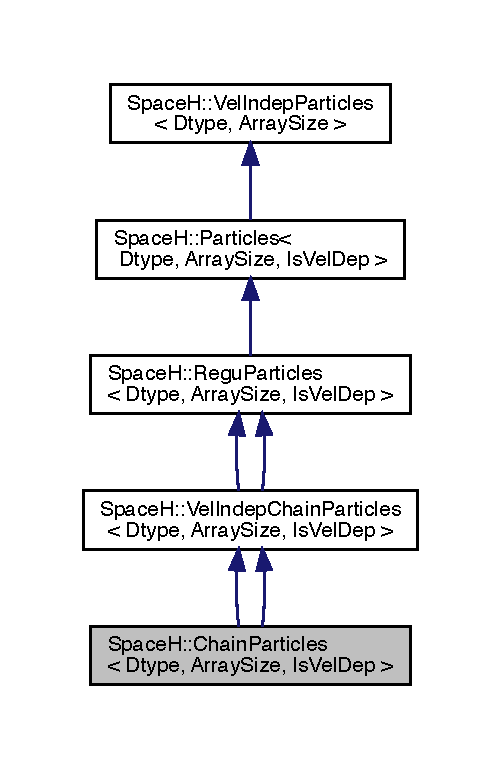
\includegraphics[width=241pt]{class_space_h_1_1_chain_particles__inherit__graph}
\end{center}
\end{figure}


Collaboration diagram for SpaceH\+:\+:Chain\+Particles$<$ Dtype, Array\+Size, Is\+Vel\+Dep $>$\+:
\nopagebreak
\begin{figure}[H]
\begin{center}
\leavevmode
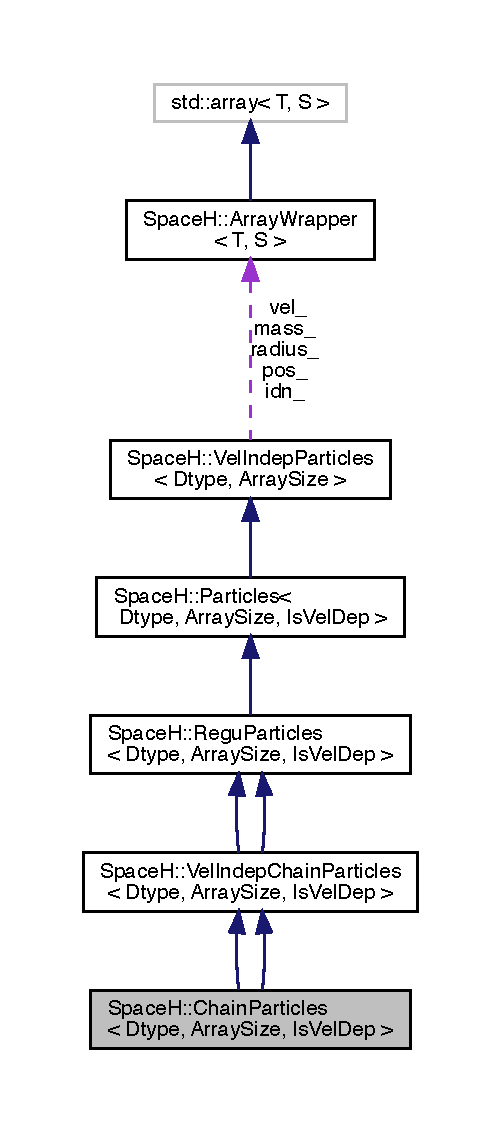
\includegraphics[width=241pt]{class_space_h_1_1_chain_particles__coll__graph}
\end{center}
\end{figure}
\subsection*{Additional Inherited Members}


The documentation for this class was generated from the following file\+:\begin{DoxyCompactItemize}
\item 
particle\+System/\+A\+R\+Chain/\mbox{\hyperlink{chain_particles_8h}{chain\+Particles.\+h}}\end{DoxyCompactItemize}

\hypertarget{class_space_h_1_1_chain_particles_3_01_dtype_00_01_array_size_00_01true_01_4}{}\section{SpaceH\+:\+:Chain\+Particles$<$ Dtype, Array\+Size, true $>$ Class Template Reference}
\label{class_space_h_1_1_chain_particles_3_01_dtype_00_01_array_size_00_01true_01_4}\index{Space\+H\+::\+Chain\+Particles$<$ Dtype, Array\+Size, true $>$@{Space\+H\+::\+Chain\+Particles$<$ Dtype, Array\+Size, true $>$}}


{\ttfamily \#include $<$chain\+Particles.\+h$>$}



Inheritance diagram for SpaceH\+:\+:Chain\+Particles$<$ Dtype, Array\+Size, true $>$\+:
\nopagebreak
\begin{figure}[H]
\begin{center}
\leavevmode
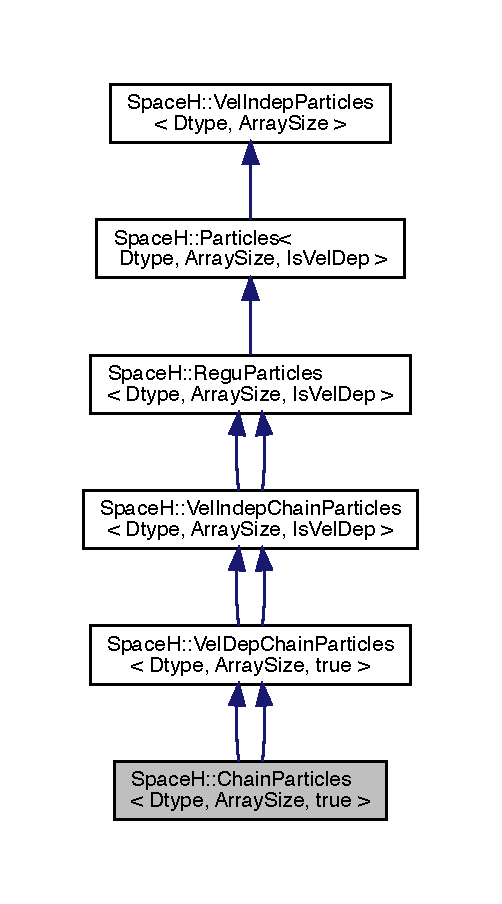
\includegraphics[width=241pt]{class_space_h_1_1_chain_particles_3_01_dtype_00_01_array_size_00_01true_01_4__inherit__graph}
\end{center}
\end{figure}


Collaboration diagram for SpaceH\+:\+:Chain\+Particles$<$ Dtype, Array\+Size, true $>$\+:
\nopagebreak
\begin{figure}[H]
\begin{center}
\leavevmode
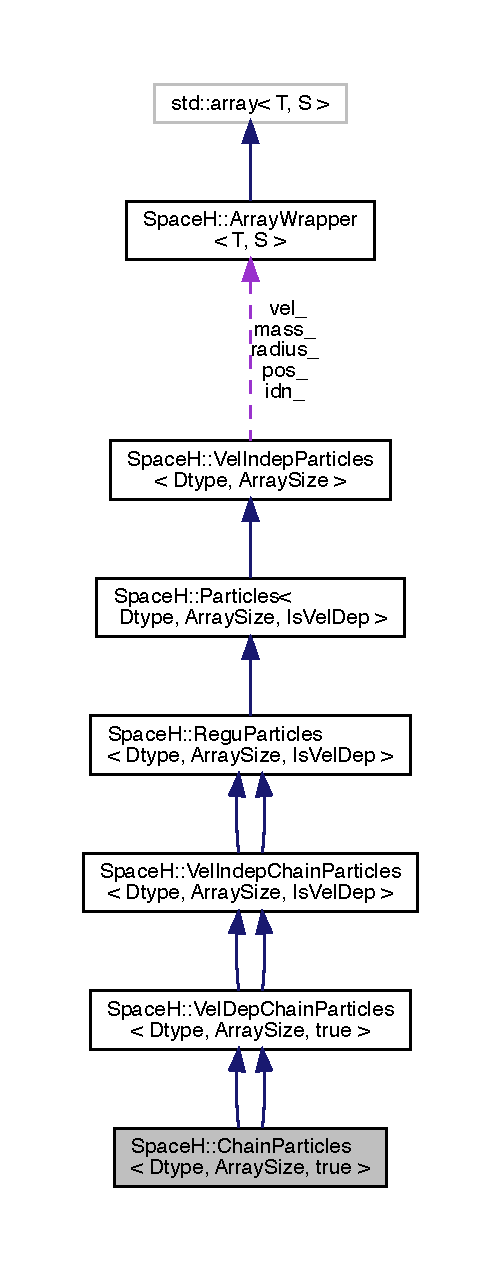
\includegraphics[height=550pt]{class_space_h_1_1_chain_particles_3_01_dtype_00_01_array_size_00_01true_01_4__coll__graph}
\end{center}
\end{figure}
\subsection*{Additional Inherited Members}


The documentation for this class was generated from the following file\+:\begin{DoxyCompactItemize}
\item 
particle\+System/\+A\+R\+Chain/\mbox{\hyperlink{chain_particles_8h}{chain\+Particles.\+h}}\end{DoxyCompactItemize}

\hypertarget{class_space_h_1_1const_iterator}{}\section{SpaceH\+:\+:const\+Iterator$<$ Partic\+Sys, Integrator $>$ Class Template Reference}
\label{class_space_h_1_1const_iterator}\index{Space\+H\+::const\+Iterator$<$ Partic\+Sys, Integrator $>$@{Space\+H\+::const\+Iterator$<$ Partic\+Sys, Integrator $>$}}


Most common iterator.  




{\ttfamily \#include $<$const\+Iterator.\+h$>$}

\subsection*{Public Types}
\begin{DoxyCompactItemize}
\item 
using \mbox{\hyperlink{class_space_h_1_1const_iterator_a2a6ca617f92a243149efe6027f1ffea2}{type}} = typename Partic\+Sys\+::type
\item 
using \mbox{\hyperlink{class_space_h_1_1const_iterator_aa8e66385a5d8eeb2a8dc98a2e1c2dbdd}{Scalar}} = typename type\+::\+Scalar
\end{DoxyCompactItemize}
\subsection*{Public Member Functions}
\begin{DoxyCompactItemize}
\item 
\mbox{\hyperlink{class_space_h_1_1const_iterator_aa8e66385a5d8eeb2a8dc98a2e1c2dbdd}{Scalar}} \mbox{\hyperlink{class_space_h_1_1const_iterator_a75d21d7e7427f6c667cd9fc954e99cc6}{iterate}} (Partic\+Sys \&particles, \mbox{\hyperlink{class_space_h_1_1const_iterator_aa8e66385a5d8eeb2a8dc98a2e1c2dbdd}{Scalar}} step\+Length)
\begin{DoxyCompactList}\small\item\em interface to iterate particle system for one step \end{DoxyCompactList}\end{DoxyCompactItemize}


\subsection{Detailed Description}
\subsubsection*{template$<$typename Partic\+Sys, typename Integrator$>$\newline
class Space\+H\+::const\+Iterator$<$ Partic\+Sys, Integrator $>$}

Most common iterator. 

Constant iterator keep the step length constant and integrate the particle system for one step. 

\subsection{Member Typedef Documentation}
\mbox{\Hypertarget{class_space_h_1_1const_iterator_aa8e66385a5d8eeb2a8dc98a2e1c2dbdd}\label{class_space_h_1_1const_iterator_aa8e66385a5d8eeb2a8dc98a2e1c2dbdd}} 
\index{Space\+H\+::const\+Iterator@{Space\+H\+::const\+Iterator}!Scalar@{Scalar}}
\index{Scalar@{Scalar}!Space\+H\+::const\+Iterator@{Space\+H\+::const\+Iterator}}
\subsubsection{\texorpdfstring{Scalar}{Scalar}}
{\footnotesize\ttfamily template$<$typename Partic\+Sys , typename Integrator $>$ \\
using \mbox{\hyperlink{class_space_h_1_1const_iterator}{Space\+H\+::const\+Iterator}}$<$ Partic\+Sys, Integrator $>$\+::\mbox{\hyperlink{class_space_h_1_1const_iterator_aa8e66385a5d8eeb2a8dc98a2e1c2dbdd}{Scalar}} =  typename type\+::\+Scalar}

\mbox{\Hypertarget{class_space_h_1_1const_iterator_a2a6ca617f92a243149efe6027f1ffea2}\label{class_space_h_1_1const_iterator_a2a6ca617f92a243149efe6027f1ffea2}} 
\index{Space\+H\+::const\+Iterator@{Space\+H\+::const\+Iterator}!type@{type}}
\index{type@{type}!Space\+H\+::const\+Iterator@{Space\+H\+::const\+Iterator}}
\subsubsection{\texorpdfstring{type}{type}}
{\footnotesize\ttfamily template$<$typename Partic\+Sys , typename Integrator $>$ \\
using \mbox{\hyperlink{class_space_h_1_1const_iterator}{Space\+H\+::const\+Iterator}}$<$ Partic\+Sys, Integrator $>$\+::\mbox{\hyperlink{class_space_h_1_1const_iterator_a2a6ca617f92a243149efe6027f1ffea2}{type}} =  typename Partic\+Sys\+::type}



\subsection{Member Function Documentation}
\mbox{\Hypertarget{class_space_h_1_1const_iterator_a75d21d7e7427f6c667cd9fc954e99cc6}\label{class_space_h_1_1const_iterator_a75d21d7e7427f6c667cd9fc954e99cc6}} 
\index{Space\+H\+::const\+Iterator@{Space\+H\+::const\+Iterator}!iterate@{iterate}}
\index{iterate@{iterate}!Space\+H\+::const\+Iterator@{Space\+H\+::const\+Iterator}}
\subsubsection{\texorpdfstring{iterate()}{iterate()}}
{\footnotesize\ttfamily template$<$typename Partic\+Sys , typename Integrator $>$ \\
\mbox{\hyperlink{class_space_h_1_1const_iterator_aa8e66385a5d8eeb2a8dc98a2e1c2dbdd}{Scalar}} \mbox{\hyperlink{class_space_h_1_1const_iterator}{Space\+H\+::const\+Iterator}}$<$ Partic\+Sys, Integrator $>$\+::iterate (\begin{DoxyParamCaption}\item[{Partic\+Sys \&}]{particles,  }\item[{\mbox{\hyperlink{class_space_h_1_1const_iterator_aa8e66385a5d8eeb2a8dc98a2e1c2dbdd}{Scalar}}}]{step\+Length }\end{DoxyParamCaption})\hspace{0.3cm}{\ttfamily [inline]}}



interface to iterate particle system for one step 


\begin{DoxyParams}{Parameters}
{\em particles} & \mbox{\hyperlink{struct_space_h_1_1_particle}{Particle}} system needs evolution. \\
\hline
{\em integrator} & Integrator to integrate the particle system. \\
\hline
{\em step\+Length} & Macro step length for iteration(\+Here, the step length of the integrator). \\
\hline
\end{DoxyParams}
\begin{DoxyReturn}{Returns}
step length for next iteration. 
\end{DoxyReturn}


The documentation for this class was generated from the following file\+:\begin{DoxyCompactItemize}
\item 
O\+D\+Eiterator/\mbox{\hyperlink{const_iterator_8h}{const\+Iterator.\+h}}\end{DoxyCompactItemize}

\hypertarget{struct_space_h_1_1_oc_tree_1_1_coord}{}\section{SpaceH\+:\+:Oc\+Tree\+:\+:Coord$<$ T $>$ Struct Template Reference}
\label{struct_space_h_1_1_oc_tree_1_1_coord}\index{Space\+H\+::\+Oc\+Tree\+::\+Coord$<$ T $>$@{Space\+H\+::\+Oc\+Tree\+::\+Coord$<$ T $>$}}


{\ttfamily \#include $<$octree.\+h$>$}

\subsection*{Public Types}
\begin{DoxyCompactItemize}
\item 
using \mbox{\hyperlink{struct_space_h_1_1_oc_tree_1_1_coord_a7d0ab8b11125aa7214690a891c682645}{value\+\_\+type}} = T
\end{DoxyCompactItemize}
\subsection*{Public Attributes}
\begin{DoxyCompactItemize}
\item 
T \mbox{\hyperlink{struct_space_h_1_1_oc_tree_1_1_coord_acaf50e31eeb18f518b0f3d8ea06c69ac}{xmin}} \{0\}
\item 
T \mbox{\hyperlink{struct_space_h_1_1_oc_tree_1_1_coord_a4cedb350f1b5cee24f8fbb435af7b2d0}{xmax}} \{0\}
\item 
T \mbox{\hyperlink{struct_space_h_1_1_oc_tree_1_1_coord_a094b49bff80734585def902f87973f15}{ymin}} \{0\}
\item 
T \mbox{\hyperlink{struct_space_h_1_1_oc_tree_1_1_coord_ae4fbed83cac15bf8aeeb4a54f21ef829}{ymax}} \{0\}
\item 
T \mbox{\hyperlink{struct_space_h_1_1_oc_tree_1_1_coord_a62fc99017cd4495c3e93f779002870e9}{zmin}} \{0\}
\item 
T \mbox{\hyperlink{struct_space_h_1_1_oc_tree_1_1_coord_aeb57e74e4175c2973f3bc5cc0b0cb120}{zmax}} \{0\}
\end{DoxyCompactItemize}


\subsection{Member Typedef Documentation}
\mbox{\Hypertarget{struct_space_h_1_1_oc_tree_1_1_coord_a7d0ab8b11125aa7214690a891c682645}\label{struct_space_h_1_1_oc_tree_1_1_coord_a7d0ab8b11125aa7214690a891c682645}} 
\index{Space\+H\+::\+Oc\+Tree\+::\+Coord@{Space\+H\+::\+Oc\+Tree\+::\+Coord}!value\+\_\+type@{value\+\_\+type}}
\index{value\+\_\+type@{value\+\_\+type}!Space\+H\+::\+Oc\+Tree\+::\+Coord@{Space\+H\+::\+Oc\+Tree\+::\+Coord}}
\subsubsection{\texorpdfstring{value\+\_\+type}{value\_type}}
{\footnotesize\ttfamily template$<$typename T$>$ \\
using \mbox{\hyperlink{struct_space_h_1_1_oc_tree_1_1_coord}{Space\+H\+::\+Oc\+Tree\+::\+Coord}}$<$ T $>$\+::\mbox{\hyperlink{struct_space_h_1_1_oc_tree_1_1_coord_a7d0ab8b11125aa7214690a891c682645}{value\+\_\+type}} =  T}



\subsection{Member Data Documentation}
\mbox{\Hypertarget{struct_space_h_1_1_oc_tree_1_1_coord_a4cedb350f1b5cee24f8fbb435af7b2d0}\label{struct_space_h_1_1_oc_tree_1_1_coord_a4cedb350f1b5cee24f8fbb435af7b2d0}} 
\index{Space\+H\+::\+Oc\+Tree\+::\+Coord@{Space\+H\+::\+Oc\+Tree\+::\+Coord}!xmax@{xmax}}
\index{xmax@{xmax}!Space\+H\+::\+Oc\+Tree\+::\+Coord@{Space\+H\+::\+Oc\+Tree\+::\+Coord}}
\subsubsection{\texorpdfstring{xmax}{xmax}}
{\footnotesize\ttfamily template$<$typename T$>$ \\
T \mbox{\hyperlink{struct_space_h_1_1_oc_tree_1_1_coord}{Space\+H\+::\+Oc\+Tree\+::\+Coord}}$<$ T $>$\+::xmax \{0\}}

\mbox{\Hypertarget{struct_space_h_1_1_oc_tree_1_1_coord_acaf50e31eeb18f518b0f3d8ea06c69ac}\label{struct_space_h_1_1_oc_tree_1_1_coord_acaf50e31eeb18f518b0f3d8ea06c69ac}} 
\index{Space\+H\+::\+Oc\+Tree\+::\+Coord@{Space\+H\+::\+Oc\+Tree\+::\+Coord}!xmin@{xmin}}
\index{xmin@{xmin}!Space\+H\+::\+Oc\+Tree\+::\+Coord@{Space\+H\+::\+Oc\+Tree\+::\+Coord}}
\subsubsection{\texorpdfstring{xmin}{xmin}}
{\footnotesize\ttfamily template$<$typename T$>$ \\
T \mbox{\hyperlink{struct_space_h_1_1_oc_tree_1_1_coord}{Space\+H\+::\+Oc\+Tree\+::\+Coord}}$<$ T $>$\+::xmin \{0\}}

\mbox{\Hypertarget{struct_space_h_1_1_oc_tree_1_1_coord_ae4fbed83cac15bf8aeeb4a54f21ef829}\label{struct_space_h_1_1_oc_tree_1_1_coord_ae4fbed83cac15bf8aeeb4a54f21ef829}} 
\index{Space\+H\+::\+Oc\+Tree\+::\+Coord@{Space\+H\+::\+Oc\+Tree\+::\+Coord}!ymax@{ymax}}
\index{ymax@{ymax}!Space\+H\+::\+Oc\+Tree\+::\+Coord@{Space\+H\+::\+Oc\+Tree\+::\+Coord}}
\subsubsection{\texorpdfstring{ymax}{ymax}}
{\footnotesize\ttfamily template$<$typename T$>$ \\
T \mbox{\hyperlink{struct_space_h_1_1_oc_tree_1_1_coord}{Space\+H\+::\+Oc\+Tree\+::\+Coord}}$<$ T $>$\+::ymax \{0\}}

\mbox{\Hypertarget{struct_space_h_1_1_oc_tree_1_1_coord_a094b49bff80734585def902f87973f15}\label{struct_space_h_1_1_oc_tree_1_1_coord_a094b49bff80734585def902f87973f15}} 
\index{Space\+H\+::\+Oc\+Tree\+::\+Coord@{Space\+H\+::\+Oc\+Tree\+::\+Coord}!ymin@{ymin}}
\index{ymin@{ymin}!Space\+H\+::\+Oc\+Tree\+::\+Coord@{Space\+H\+::\+Oc\+Tree\+::\+Coord}}
\subsubsection{\texorpdfstring{ymin}{ymin}}
{\footnotesize\ttfamily template$<$typename T$>$ \\
T \mbox{\hyperlink{struct_space_h_1_1_oc_tree_1_1_coord}{Space\+H\+::\+Oc\+Tree\+::\+Coord}}$<$ T $>$\+::ymin \{0\}}

\mbox{\Hypertarget{struct_space_h_1_1_oc_tree_1_1_coord_aeb57e74e4175c2973f3bc5cc0b0cb120}\label{struct_space_h_1_1_oc_tree_1_1_coord_aeb57e74e4175c2973f3bc5cc0b0cb120}} 
\index{Space\+H\+::\+Oc\+Tree\+::\+Coord@{Space\+H\+::\+Oc\+Tree\+::\+Coord}!zmax@{zmax}}
\index{zmax@{zmax}!Space\+H\+::\+Oc\+Tree\+::\+Coord@{Space\+H\+::\+Oc\+Tree\+::\+Coord}}
\subsubsection{\texorpdfstring{zmax}{zmax}}
{\footnotesize\ttfamily template$<$typename T$>$ \\
T \mbox{\hyperlink{struct_space_h_1_1_oc_tree_1_1_coord}{Space\+H\+::\+Oc\+Tree\+::\+Coord}}$<$ T $>$\+::zmax \{0\}}

\mbox{\Hypertarget{struct_space_h_1_1_oc_tree_1_1_coord_a62fc99017cd4495c3e93f779002870e9}\label{struct_space_h_1_1_oc_tree_1_1_coord_a62fc99017cd4495c3e93f779002870e9}} 
\index{Space\+H\+::\+Oc\+Tree\+::\+Coord@{Space\+H\+::\+Oc\+Tree\+::\+Coord}!zmin@{zmin}}
\index{zmin@{zmin}!Space\+H\+::\+Oc\+Tree\+::\+Coord@{Space\+H\+::\+Oc\+Tree\+::\+Coord}}
\subsubsection{\texorpdfstring{zmin}{zmin}}
{\footnotesize\ttfamily template$<$typename T$>$ \\
T \mbox{\hyperlink{struct_space_h_1_1_oc_tree_1_1_coord}{Space\+H\+::\+Oc\+Tree\+::\+Coord}}$<$ T $>$\+::zmin \{0\}}



The documentation for this struct was generated from the following file\+:\begin{DoxyCompactItemize}
\item 
particle\+System/octree/\mbox{\hyperlink{octree_8h}{octree.\+h}}\end{DoxyCompactItemize}

\hypertarget{classdicho_iterator}{}\section{dicho\+Iterator$<$ Partic\+Sys, Integrator $>$ Class Template Reference}
\label{classdicho_iterator}\index{dicho\+Iterator$<$ Partic\+Sys, Integrator $>$@{dicho\+Iterator$<$ Partic\+Sys, Integrator $>$}}


Dichotomy iterator.  




{\ttfamily \#include $<$dichotomy.\+h$>$}

\subsection*{Public Types}
\begin{DoxyCompactItemize}
\item 
typedef Partic\+Sys\+::\+Scalar \mbox{\hyperlink{classdicho_iterator_a292e986136313822f21b1b60d9cbb95d}{Scalar}}
\item 
typedef Partic\+Sys\+::\+Plain\+Array \mbox{\hyperlink{classdicho_iterator_ab5b708b3b8a8fbd975c55231052d2547}{Plain\+Array}}
\end{DoxyCompactItemize}
\subsection*{Public Member Functions}
\begin{DoxyCompactItemize}
\item 
\mbox{\hyperlink{classdicho_iterator_a292e986136313822f21b1b60d9cbb95d}{Scalar}} \mbox{\hyperlink{classdicho_iterator_ad341b0652d8fb1530707893ed48a0257}{iterate}} (Partic\+Sys \&particles, \mbox{\hyperlink{classdicho_iterator_a292e986136313822f21b1b60d9cbb95d}{Scalar}} step\+Length)
\begin{DoxyCompactList}\small\item\em interface to iterate particle system for one step \end{DoxyCompactList}\item 
void \mbox{\hyperlink{classdicho_iterator_a2e810ce79342069faafde863d4876ce4}{set\+Relative\+Error}} (\mbox{\hyperlink{classdicho_iterator_a292e986136313822f21b1b60d9cbb95d}{Scalar}} rel\+Error)
\begin{DoxyCompactList}\small\item\em Set the local relative error. \end{DoxyCompactList}\item 
void \mbox{\hyperlink{classdicho_iterator_a95eaed5747897df265b2935a13eee8ca}{set\+Absolute\+Error}} (\mbox{\hyperlink{classdicho_iterator_a292e986136313822f21b1b60d9cbb95d}{Scalar}} abs\+Error)
\begin{DoxyCompactList}\small\item\em Set the local absolute error. \end{DoxyCompactList}\end{DoxyCompactItemize}


\subsection{Detailed Description}
\subsubsection*{template$<$typename Partic\+Sys, typename Integrator$>$\newline
class dicho\+Iterator$<$ Partic\+Sys, Integrator $>$}

Dichotomy iterator. 

Dichotomy iterator, use dichotomy to adjust the step size. 

\subsection{Member Typedef Documentation}
\mbox{\Hypertarget{classdicho_iterator_ab5b708b3b8a8fbd975c55231052d2547}\label{classdicho_iterator_ab5b708b3b8a8fbd975c55231052d2547}} 
\index{dicho\+Iterator@{dicho\+Iterator}!Plain\+Array@{Plain\+Array}}
\index{Plain\+Array@{Plain\+Array}!dicho\+Iterator@{dicho\+Iterator}}
\subsubsection{\texorpdfstring{Plain\+Array}{PlainArray}}
{\footnotesize\ttfamily template$<$typename Partic\+Sys , typename Integrator $>$ \\
typedef Partic\+Sys\+::\+Plain\+Array \mbox{\hyperlink{classdicho_iterator}{dicho\+Iterator}}$<$ Partic\+Sys, Integrator $>$\+::\mbox{\hyperlink{classdicho_iterator_ab5b708b3b8a8fbd975c55231052d2547}{Plain\+Array}}}

\mbox{\Hypertarget{classdicho_iterator_a292e986136313822f21b1b60d9cbb95d}\label{classdicho_iterator_a292e986136313822f21b1b60d9cbb95d}} 
\index{dicho\+Iterator@{dicho\+Iterator}!Scalar@{Scalar}}
\index{Scalar@{Scalar}!dicho\+Iterator@{dicho\+Iterator}}
\subsubsection{\texorpdfstring{Scalar}{Scalar}}
{\footnotesize\ttfamily template$<$typename Partic\+Sys , typename Integrator $>$ \\
typedef Partic\+Sys\+::\+Scalar \mbox{\hyperlink{classdicho_iterator}{dicho\+Iterator}}$<$ Partic\+Sys, Integrator $>$\+::\mbox{\hyperlink{classdicho_iterator_a292e986136313822f21b1b60d9cbb95d}{Scalar}}}



\subsection{Member Function Documentation}
\mbox{\Hypertarget{classdicho_iterator_ad341b0652d8fb1530707893ed48a0257}\label{classdicho_iterator_ad341b0652d8fb1530707893ed48a0257}} 
\index{dicho\+Iterator@{dicho\+Iterator}!iterate@{iterate}}
\index{iterate@{iterate}!dicho\+Iterator@{dicho\+Iterator}}
\subsubsection{\texorpdfstring{iterate()}{iterate()}}
{\footnotesize\ttfamily template$<$typename Partic\+Sys , typename Integrator $>$ \\
\mbox{\hyperlink{test_orbit_8cpp_a8c2981f3f834be9448a6ab06c28748eb}{Partic\+Sys\+::\+Scalar}} \mbox{\hyperlink{classdicho_iterator}{dicho\+Iterator}}$<$ Partic\+Sys, Integrator $>$\+::iterate (\begin{DoxyParamCaption}\item[{Partic\+Sys \&}]{particles,  }\item[{\mbox{\hyperlink{classdicho_iterator_a292e986136313822f21b1b60d9cbb95d}{Scalar}}}]{step\+Length }\end{DoxyParamCaption})}



interface to iterate particle system for one step 


\begin{DoxyParams}{Parameters}
{\em particles} & Particle system needs evolution. \\
\hline
{\em integrator} & Integrator to integrate the particle system. \\
\hline
{\em step\+Length} & Macro step length for iteration(\+Here, the step length of the integrator). \\
\hline
\end{DoxyParams}
\begin{DoxyReturn}{Returns}
step length for next iteration. 
\end{DoxyReturn}
\mbox{\Hypertarget{classdicho_iterator_a95eaed5747897df265b2935a13eee8ca}\label{classdicho_iterator_a95eaed5747897df265b2935a13eee8ca}} 
\index{dicho\+Iterator@{dicho\+Iterator}!set\+Absolute\+Error@{set\+Absolute\+Error}}
\index{set\+Absolute\+Error@{set\+Absolute\+Error}!dicho\+Iterator@{dicho\+Iterator}}
\subsubsection{\texorpdfstring{set\+Absolute\+Error()}{setAbsoluteError()}}
{\footnotesize\ttfamily template$<$typename Partic\+Sys , typename Integrator $>$ \\
void \mbox{\hyperlink{classdicho_iterator}{dicho\+Iterator}}$<$ Partic\+Sys, Integrator $>$\+::set\+Absolute\+Error (\begin{DoxyParamCaption}\item[{\mbox{\hyperlink{classdicho_iterator_a292e986136313822f21b1b60d9cbb95d}{Scalar}}}]{abs\+Error }\end{DoxyParamCaption})\hspace{0.3cm}{\ttfamily [inline]}}



Set the local absolute error. 

\mbox{\Hypertarget{classdicho_iterator_a2e810ce79342069faafde863d4876ce4}\label{classdicho_iterator_a2e810ce79342069faafde863d4876ce4}} 
\index{dicho\+Iterator@{dicho\+Iterator}!set\+Relative\+Error@{set\+Relative\+Error}}
\index{set\+Relative\+Error@{set\+Relative\+Error}!dicho\+Iterator@{dicho\+Iterator}}
\subsubsection{\texorpdfstring{set\+Relative\+Error()}{setRelativeError()}}
{\footnotesize\ttfamily template$<$typename Partic\+Sys , typename Integrator $>$ \\
void \mbox{\hyperlink{classdicho_iterator}{dicho\+Iterator}}$<$ Partic\+Sys, Integrator $>$\+::set\+Relative\+Error (\begin{DoxyParamCaption}\item[{\mbox{\hyperlink{classdicho_iterator_a292e986136313822f21b1b60d9cbb95d}{Scalar}}}]{rel\+Error }\end{DoxyParamCaption})\hspace{0.3cm}{\ttfamily [inline]}}



Set the local relative error. 



The documentation for this class was generated from the following file\+:\begin{DoxyCompactItemize}
\item 
O\+D\+Eiterator/\mbox{\hyperlink{dichotomy_8h}{dichotomy.\+h}}\end{DoxyCompactItemize}

\hypertarget{struct_space_h_1_1_empty_class}{}\section{SpaceH\+:\+:Empty\+Class Struct Reference}
\label{struct_space_h_1_1_empty_class}\index{Space\+H\+::\+Empty\+Class@{Space\+H\+::\+Empty\+Class}}


{\ttfamily \#include $<$proto\+Type.\+h$>$}



The documentation for this struct was generated from the following file\+:\begin{DoxyCompactItemize}
\item 
\mbox{\hyperlink{proto_type_8h}{proto\+Type.\+h}}\end{DoxyCompactItemize}

\hypertarget{struct_space_h_1_1_oc_tree_1_1empty_parent_node}{}\section{SpaceH\+:\+:Oc\+Tree\+:\+:empty\+Parent\+Node$<$ T $>$ Struct Template Reference}
\label{struct_space_h_1_1_oc_tree_1_1empty_parent_node}\index{Space\+H\+::\+Oc\+Tree\+::empty\+Parent\+Node$<$ T $>$@{Space\+H\+::\+Oc\+Tree\+::empty\+Parent\+Node$<$ T $>$}}


{\ttfamily \#include $<$octree.\+h$>$}

\subsection*{Public Member Functions}
\begin{DoxyCompactItemize}
\item 
T $\ast$ \mbox{\hyperlink{struct_space_h_1_1_oc_tree_1_1empty_parent_node_aae8bd4358998eca0a7b1a5005c0bb492}{operator()}} (T $\ast$data\+Set)
\end{DoxyCompactItemize}


\subsection{Member Function Documentation}
\mbox{\Hypertarget{struct_space_h_1_1_oc_tree_1_1empty_parent_node_aae8bd4358998eca0a7b1a5005c0bb492}\label{struct_space_h_1_1_oc_tree_1_1empty_parent_node_aae8bd4358998eca0a7b1a5005c0bb492}} 
\index{Space\+H\+::\+Oc\+Tree\+::empty\+Parent\+Node@{Space\+H\+::\+Oc\+Tree\+::empty\+Parent\+Node}!operator()@{operator()}}
\index{operator()@{operator()}!Space\+H\+::\+Oc\+Tree\+::empty\+Parent\+Node@{Space\+H\+::\+Oc\+Tree\+::empty\+Parent\+Node}}
\subsubsection{\texorpdfstring{operator()()}{operator()()}}
{\footnotesize\ttfamily template$<$typename T $>$ \\
T$\ast$ \mbox{\hyperlink{struct_space_h_1_1_oc_tree_1_1empty_parent_node}{Space\+H\+::\+Oc\+Tree\+::empty\+Parent\+Node}}$<$ T $>$\+::operator() (\begin{DoxyParamCaption}\item[{T $\ast$}]{data\+Set }\end{DoxyParamCaption})\hspace{0.3cm}{\ttfamily [inline]}}



The documentation for this struct was generated from the following file\+:\begin{DoxyCompactItemize}
\item 
particle\+System/octree/\mbox{\hyperlink{octree_8h}{octree.\+h}}\end{DoxyCompactItemize}

\hypertarget{struct_space_h_1_1epsilon}{}\section{SpaceH\+:\+:epsilon$<$ Dtype $>$ Struct Template Reference}
\label{struct_space_h_1_1epsilon}\index{Space\+H\+::epsilon$<$ Dtype $>$@{Space\+H\+::epsilon$<$ Dtype $>$}}


{\ttfamily \#include $<$own\+Math.\+h$>$}

\subsection*{Public Types}
\begin{DoxyCompactItemize}
\item 
using \mbox{\hyperlink{struct_space_h_1_1epsilon_abd3cad02e7f97ff8ed6b20b67c2ff1fc}{value\+\_\+type}} = typename \mbox{\hyperlink{struct_space_h_1_1get__value__type}{Space\+H\+::get\+\_\+value\+\_\+type}}$<$ Dtype $>$\+::type
\end{DoxyCompactItemize}
\subsection*{Static Public Attributes}
\begin{DoxyCompactItemize}
\item 
static constexpr \mbox{\hyperlink{struct_space_h_1_1epsilon_abd3cad02e7f97ff8ed6b20b67c2ff1fc}{value\+\_\+type}} \mbox{\hyperlink{struct_space_h_1_1epsilon_ac5843bdc3a64016722e87809ead426bb}{value}} = std\+::numeric\+\_\+limits$<$\mbox{\hyperlink{struct_space_h_1_1epsilon_abd3cad02e7f97ff8ed6b20b67c2ff1fc}{value\+\_\+type}}$>$\+::\mbox{\hyperlink{struct_space_h_1_1epsilon}{epsilon}}()
\end{DoxyCompactItemize}


\subsection{Member Typedef Documentation}
\mbox{\Hypertarget{struct_space_h_1_1epsilon_abd3cad02e7f97ff8ed6b20b67c2ff1fc}\label{struct_space_h_1_1epsilon_abd3cad02e7f97ff8ed6b20b67c2ff1fc}} 
\index{Space\+H\+::epsilon@{Space\+H\+::epsilon}!value\+\_\+type@{value\+\_\+type}}
\index{value\+\_\+type@{value\+\_\+type}!Space\+H\+::epsilon@{Space\+H\+::epsilon}}
\subsubsection{\texorpdfstring{value\+\_\+type}{value\_type}}
{\footnotesize\ttfamily template$<$typename Dtype $>$ \\
using \mbox{\hyperlink{struct_space_h_1_1epsilon}{Space\+H\+::epsilon}}$<$ Dtype $>$\+::\mbox{\hyperlink{struct_space_h_1_1epsilon_abd3cad02e7f97ff8ed6b20b67c2ff1fc}{value\+\_\+type}} =  typename \mbox{\hyperlink{struct_space_h_1_1get__value__type}{Space\+H\+::get\+\_\+value\+\_\+type}}$<$Dtype$>$\+::type}



\subsection{Member Data Documentation}
\mbox{\Hypertarget{struct_space_h_1_1epsilon_ac5843bdc3a64016722e87809ead426bb}\label{struct_space_h_1_1epsilon_ac5843bdc3a64016722e87809ead426bb}} 
\index{Space\+H\+::epsilon@{Space\+H\+::epsilon}!value@{value}}
\index{value@{value}!Space\+H\+::epsilon@{Space\+H\+::epsilon}}
\subsubsection{\texorpdfstring{value}{value}}
{\footnotesize\ttfamily template$<$typename Dtype $>$ \\
constexpr \mbox{\hyperlink{struct_space_h_1_1epsilon_abd3cad02e7f97ff8ed6b20b67c2ff1fc}{value\+\_\+type}} \mbox{\hyperlink{struct_space_h_1_1epsilon}{Space\+H\+::epsilon}}$<$ Dtype $>$\+::value = std\+::numeric\+\_\+limits$<$\mbox{\hyperlink{struct_space_h_1_1epsilon_abd3cad02e7f97ff8ed6b20b67c2ff1fc}{value\+\_\+type}}$>$\+::\mbox{\hyperlink{struct_space_h_1_1epsilon}{epsilon}}()\hspace{0.3cm}{\ttfamily [static]}}



The documentation for this struct was generated from the following file\+:\begin{DoxyCompactItemize}
\item 
\mbox{\hyperlink{own_math_8h}{own\+Math.\+h}}\end{DoxyCompactItemize}

\hypertarget{struct_space_h_1_1_ext_vel_dep_force}{}\section{SpaceH\+:\+:Ext\+Vel\+Dep\+Force$<$ Ext\+Force, Dtype, Array\+Size $>$ Struct Template Reference}
\label{struct_space_h_1_1_ext_vel_dep_force}\index{Space\+H\+::\+Ext\+Vel\+Dep\+Force$<$ Ext\+Force, Dtype, Array\+Size $>$@{Space\+H\+::\+Ext\+Vel\+Dep\+Force$<$ Ext\+Force, Dtype, Array\+Size $>$}}


{\ttfamily \#include $<$force.\+h$>$}



Inheritance diagram for SpaceH\+:\+:Ext\+Vel\+Dep\+Force$<$ Ext\+Force, Dtype, Array\+Size $>$\+:\nopagebreak
\begin{figure}[H]
\begin{center}
\leavevmode
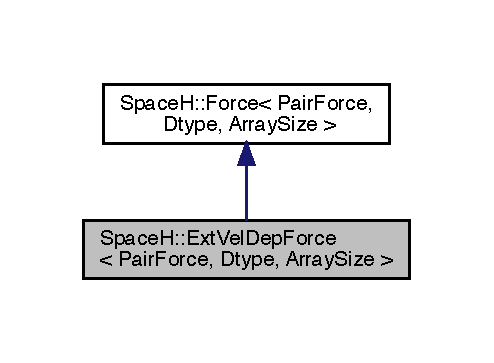
\includegraphics[width=237pt]{struct_space_h_1_1_ext_vel_dep_force__inherit__graph}
\end{center}
\end{figure}


Collaboration diagram for SpaceH\+:\+:Ext\+Vel\+Dep\+Force$<$ Ext\+Force, Dtype, Array\+Size $>$\+:\nopagebreak
\begin{figure}[H]
\begin{center}
\leavevmode
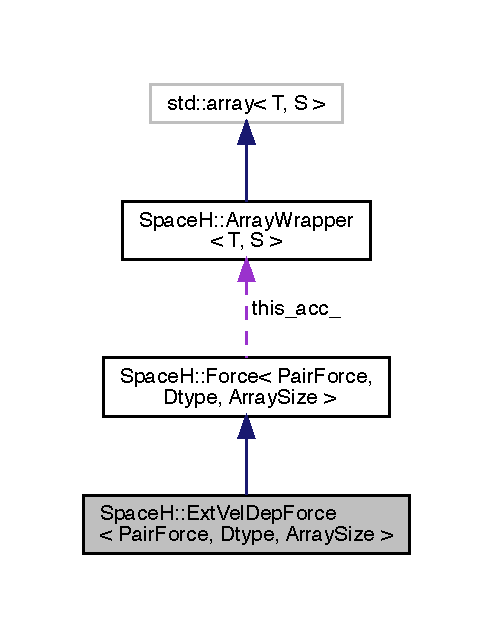
\includegraphics[width=237pt]{struct_space_h_1_1_ext_vel_dep_force__coll__graph}
\end{center}
\end{figure}
\subsection*{Public Types}
\begin{DoxyCompactItemize}
\item 
using \mbox{\hyperlink{struct_space_h_1_1_ext_vel_dep_force_a92ddc0ad1001e17ef8b4f870be20cada}{Base}} = \mbox{\hyperlink{struct_space_h_1_1_force}{Force}}$<$ Ext\+Force, Dtype, Array\+Size $>$
\item 
using \mbox{\hyperlink{struct_space_h_1_1_ext_vel_dep_force_ace51228267cd84b498bef72f6a06b727}{type}} = typename \mbox{\hyperlink{struct_space_h_1_1_force_a151c6ae1ec7ad87825c2b6cc74aee5f2}{Base\+::type}}
\item 
using \mbox{\hyperlink{struct_space_h_1_1_ext_vel_dep_force_afb0d9418e7236855d8cd8ce883493c27}{Scalar\+Array}} = typename type\+::\+Scalar\+Array
\item 
using \mbox{\hyperlink{struct_space_h_1_1_ext_vel_dep_force_ac2320cdd3fdaad369c901e79ded11d31}{Vector\+Array}} = typename type\+::\+Vector\+Array
\end{DoxyCompactItemize}
\subsection*{Public Member Functions}
\begin{DoxyCompactItemize}
\item 
void \mbox{\hyperlink{struct_space_h_1_1_ext_vel_dep_force_a58775894138f5ebd1d7d7460183f6c1e}{calcu\+Acc}} (const \mbox{\hyperlink{struct_space_h_1_1_ext_vel_dep_force_afb0d9418e7236855d8cd8ce883493c27}{Scalar\+Array}} \&mass, const \mbox{\hyperlink{struct_space_h_1_1_ext_vel_dep_force_ac2320cdd3fdaad369c901e79ded11d31}{Vector\+Array}} \&pos, const \mbox{\hyperlink{struct_space_h_1_1_ext_vel_dep_force_ac2320cdd3fdaad369c901e79ded11d31}{Vector\+Array}} \&vel)
\end{DoxyCompactItemize}
\subsection*{Additional Inherited Members}


\subsection{Member Typedef Documentation}
\mbox{\Hypertarget{struct_space_h_1_1_ext_vel_dep_force_a92ddc0ad1001e17ef8b4f870be20cada}\label{struct_space_h_1_1_ext_vel_dep_force_a92ddc0ad1001e17ef8b4f870be20cada}} 
\index{Space\+H\+::\+Ext\+Vel\+Dep\+Force@{Space\+H\+::\+Ext\+Vel\+Dep\+Force}!Base@{Base}}
\index{Base@{Base}!Space\+H\+::\+Ext\+Vel\+Dep\+Force@{Space\+H\+::\+Ext\+Vel\+Dep\+Force}}
\subsubsection{\texorpdfstring{Base}{Base}}
{\footnotesize\ttfamily template$<$typename Ext\+Force, typename Dtype, size\+\_\+t Array\+Size$>$ \\
using \mbox{\hyperlink{struct_space_h_1_1_ext_vel_dep_force}{Space\+H\+::\+Ext\+Vel\+Dep\+Force}}$<$ Ext\+Force, Dtype, Array\+Size $>$\+::\mbox{\hyperlink{struct_space_h_1_1_ext_vel_dep_force_a92ddc0ad1001e17ef8b4f870be20cada}{Base}} =  \mbox{\hyperlink{struct_space_h_1_1_force}{Force}}$<$Ext\+Force, Dtype, Array\+Size$>$}

\mbox{\Hypertarget{struct_space_h_1_1_ext_vel_dep_force_afb0d9418e7236855d8cd8ce883493c27}\label{struct_space_h_1_1_ext_vel_dep_force_afb0d9418e7236855d8cd8ce883493c27}} 
\index{Space\+H\+::\+Ext\+Vel\+Dep\+Force@{Space\+H\+::\+Ext\+Vel\+Dep\+Force}!Scalar\+Array@{Scalar\+Array}}
\index{Scalar\+Array@{Scalar\+Array}!Space\+H\+::\+Ext\+Vel\+Dep\+Force@{Space\+H\+::\+Ext\+Vel\+Dep\+Force}}
\subsubsection{\texorpdfstring{Scalar\+Array}{ScalarArray}}
{\footnotesize\ttfamily template$<$typename Ext\+Force, typename Dtype, size\+\_\+t Array\+Size$>$ \\
using \mbox{\hyperlink{struct_space_h_1_1_ext_vel_dep_force}{Space\+H\+::\+Ext\+Vel\+Dep\+Force}}$<$ Ext\+Force, Dtype, Array\+Size $>$\+::\mbox{\hyperlink{struct_space_h_1_1_ext_vel_dep_force_afb0d9418e7236855d8cd8ce883493c27}{Scalar\+Array}} =  typename type\+::\+Scalar\+Array}

\mbox{\Hypertarget{struct_space_h_1_1_ext_vel_dep_force_ace51228267cd84b498bef72f6a06b727}\label{struct_space_h_1_1_ext_vel_dep_force_ace51228267cd84b498bef72f6a06b727}} 
\index{Space\+H\+::\+Ext\+Vel\+Dep\+Force@{Space\+H\+::\+Ext\+Vel\+Dep\+Force}!type@{type}}
\index{type@{type}!Space\+H\+::\+Ext\+Vel\+Dep\+Force@{Space\+H\+::\+Ext\+Vel\+Dep\+Force}}
\subsubsection{\texorpdfstring{type}{type}}
{\footnotesize\ttfamily template$<$typename Ext\+Force, typename Dtype, size\+\_\+t Array\+Size$>$ \\
using \mbox{\hyperlink{struct_space_h_1_1_ext_vel_dep_force}{Space\+H\+::\+Ext\+Vel\+Dep\+Force}}$<$ Ext\+Force, Dtype, Array\+Size $>$\+::\mbox{\hyperlink{struct_space_h_1_1_ext_vel_dep_force_ace51228267cd84b498bef72f6a06b727}{type}} =  typename \mbox{\hyperlink{struct_space_h_1_1_force_a151c6ae1ec7ad87825c2b6cc74aee5f2}{Base\+::type}}}

\mbox{\Hypertarget{struct_space_h_1_1_ext_vel_dep_force_ac2320cdd3fdaad369c901e79ded11d31}\label{struct_space_h_1_1_ext_vel_dep_force_ac2320cdd3fdaad369c901e79ded11d31}} 
\index{Space\+H\+::\+Ext\+Vel\+Dep\+Force@{Space\+H\+::\+Ext\+Vel\+Dep\+Force}!Vector\+Array@{Vector\+Array}}
\index{Vector\+Array@{Vector\+Array}!Space\+H\+::\+Ext\+Vel\+Dep\+Force@{Space\+H\+::\+Ext\+Vel\+Dep\+Force}}
\subsubsection{\texorpdfstring{Vector\+Array}{VectorArray}}
{\footnotesize\ttfamily template$<$typename Ext\+Force, typename Dtype, size\+\_\+t Array\+Size$>$ \\
using \mbox{\hyperlink{struct_space_h_1_1_ext_vel_dep_force}{Space\+H\+::\+Ext\+Vel\+Dep\+Force}}$<$ Ext\+Force, Dtype, Array\+Size $>$\+::\mbox{\hyperlink{struct_space_h_1_1_ext_vel_dep_force_ac2320cdd3fdaad369c901e79ded11d31}{Vector\+Array}} =  typename type\+::\+Vector\+Array}



\subsection{Member Function Documentation}
\mbox{\Hypertarget{struct_space_h_1_1_ext_vel_dep_force_a58775894138f5ebd1d7d7460183f6c1e}\label{struct_space_h_1_1_ext_vel_dep_force_a58775894138f5ebd1d7d7460183f6c1e}} 
\index{Space\+H\+::\+Ext\+Vel\+Dep\+Force@{Space\+H\+::\+Ext\+Vel\+Dep\+Force}!calcu\+Acc@{calcu\+Acc}}
\index{calcu\+Acc@{calcu\+Acc}!Space\+H\+::\+Ext\+Vel\+Dep\+Force@{Space\+H\+::\+Ext\+Vel\+Dep\+Force}}
\subsubsection{\texorpdfstring{calcu\+Acc()}{calcuAcc()}}
{\footnotesize\ttfamily template$<$typename Ext\+Force, typename Dtype, size\+\_\+t Array\+Size$>$ \\
void \mbox{\hyperlink{struct_space_h_1_1_ext_vel_dep_force}{Space\+H\+::\+Ext\+Vel\+Dep\+Force}}$<$ Ext\+Force, Dtype, Array\+Size $>$\+::calcu\+Acc (\begin{DoxyParamCaption}\item[{const \mbox{\hyperlink{struct_space_h_1_1_ext_vel_dep_force_afb0d9418e7236855d8cd8ce883493c27}{Scalar\+Array}} \&}]{mass,  }\item[{const \mbox{\hyperlink{struct_space_h_1_1_ext_vel_dep_force_ac2320cdd3fdaad369c901e79ded11d31}{Vector\+Array}} \&}]{pos,  }\item[{const \mbox{\hyperlink{struct_space_h_1_1_ext_vel_dep_force_ac2320cdd3fdaad369c901e79ded11d31}{Vector\+Array}} \&}]{vel }\end{DoxyParamCaption})\hspace{0.3cm}{\ttfamily [inline]}}

Here is the caller graph for this function\+:
\nopagebreak
\begin{figure}[H]
\begin{center}
\leavevmode
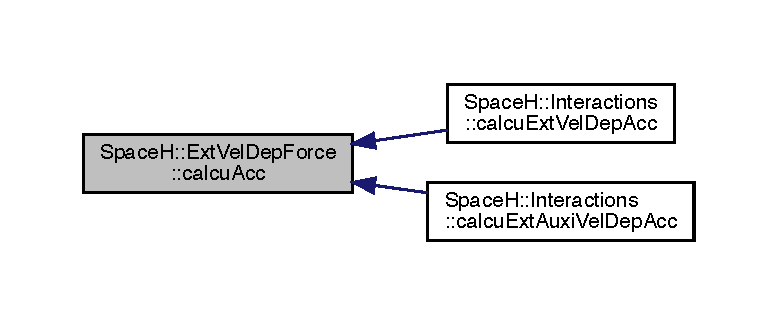
\includegraphics[width=350pt]{struct_space_h_1_1_ext_vel_dep_force_a58775894138f5ebd1d7d7460183f6c1e_icgraph}
\end{center}
\end{figure}


The documentation for this struct was generated from the following file\+:\begin{DoxyCompactItemize}
\item 
interaction/\mbox{\hyperlink{force_8h}{force.\+h}}\end{DoxyCompactItemize}

\hypertarget{struct_space_h_1_1_ext_vel_dep_force_3_01void_00_01_dtype_00_01_array_size_01_4}{}\section{SpaceH\+:\+:Ext\+Vel\+Dep\+Force$<$ void, Dtype, Array\+Size $>$ Struct Template Reference}
\label{struct_space_h_1_1_ext_vel_dep_force_3_01void_00_01_dtype_00_01_array_size_01_4}\index{Space\+H\+::\+Ext\+Vel\+Dep\+Force$<$ void, Dtype, Array\+Size $>$@{Space\+H\+::\+Ext\+Vel\+Dep\+Force$<$ void, Dtype, Array\+Size $>$}}


{\ttfamily \#include $<$force.\+h$>$}

\subsection*{Public Types}
\begin{DoxyCompactItemize}
\item 
using \mbox{\hyperlink{struct_space_h_1_1_ext_vel_dep_force_3_01void_00_01_dtype_00_01_array_size_01_4_a6f1a7483c68f9269a6313400c93e774a}{type}} = \mbox{\hyperlink{struct_space_h_1_1_proto_type}{Space\+H\+::\+Proto\+Type}}$<$ Dtype, Array\+Size $>$
\item 
using \mbox{\hyperlink{struct_space_h_1_1_ext_vel_dep_force_3_01void_00_01_dtype_00_01_array_size_01_4_aff7fedbfa20cab198234cc35a922fa1f}{Scalar\+Array}} = typename \mbox{\hyperlink{struct_space_h_1_1_proto_type_a09ef91dc8a37a044c403f5a833044725}{type\+::\+Scalar\+Array}}
\item 
using \mbox{\hyperlink{struct_space_h_1_1_ext_vel_dep_force_3_01void_00_01_dtype_00_01_array_size_01_4_a606b1df4989b62f06775a825c0f8e483}{Vector\+Array}} = typename \mbox{\hyperlink{struct_space_h_1_1_proto_type_a622b8e122b33bb4966a02299fb7b82d6}{type\+::\+Vector\+Array}}
\end{DoxyCompactItemize}
\subsection*{Public Member Functions}
\begin{DoxyCompactItemize}
\item 
void \mbox{\hyperlink{struct_space_h_1_1_ext_vel_dep_force_3_01void_00_01_dtype_00_01_array_size_01_4_ace1007ee6131097df834217979940cbb}{add\+Total}} (\mbox{\hyperlink{struct_space_h_1_1_ext_vel_dep_force_3_01void_00_01_dtype_00_01_array_size_01_4_a606b1df4989b62f06775a825c0f8e483}{Vector\+Array}} \&acc)
\item 
void \mbox{\hyperlink{struct_space_h_1_1_ext_vel_dep_force_3_01void_00_01_dtype_00_01_array_size_01_4_ab1ab7d0fa69ef28c8ec05ce5673d3373}{calcu\+Acc}} (const \mbox{\hyperlink{struct_space_h_1_1_ext_vel_dep_force_3_01void_00_01_dtype_00_01_array_size_01_4_aff7fedbfa20cab198234cc35a922fa1f}{Scalar\+Array}} \&mass, const \mbox{\hyperlink{struct_space_h_1_1_ext_vel_dep_force_3_01void_00_01_dtype_00_01_array_size_01_4_a606b1df4989b62f06775a825c0f8e483}{Vector\+Array}} \&pos, const \mbox{\hyperlink{struct_space_h_1_1_ext_vel_dep_force_3_01void_00_01_dtype_00_01_array_size_01_4_a606b1df4989b62f06775a825c0f8e483}{Vector\+Array}} \&vel)
\end{DoxyCompactItemize}


\subsection{Member Typedef Documentation}
\mbox{\Hypertarget{struct_space_h_1_1_ext_vel_dep_force_3_01void_00_01_dtype_00_01_array_size_01_4_aff7fedbfa20cab198234cc35a922fa1f}\label{struct_space_h_1_1_ext_vel_dep_force_3_01void_00_01_dtype_00_01_array_size_01_4_aff7fedbfa20cab198234cc35a922fa1f}} 
\index{Space\+H\+::\+Ext\+Vel\+Dep\+Force$<$ void, Dtype, Array\+Size $>$@{Space\+H\+::\+Ext\+Vel\+Dep\+Force$<$ void, Dtype, Array\+Size $>$}!Scalar\+Array@{Scalar\+Array}}
\index{Scalar\+Array@{Scalar\+Array}!Space\+H\+::\+Ext\+Vel\+Dep\+Force$<$ void, Dtype, Array\+Size $>$@{Space\+H\+::\+Ext\+Vel\+Dep\+Force$<$ void, Dtype, Array\+Size $>$}}
\subsubsection{\texorpdfstring{Scalar\+Array}{ScalarArray}}
{\footnotesize\ttfamily template$<$typename Dtype , size\+\_\+t Array\+Size$>$ \\
using \mbox{\hyperlink{struct_space_h_1_1_ext_vel_dep_force}{Space\+H\+::\+Ext\+Vel\+Dep\+Force}}$<$ void, Dtype, Array\+Size $>$\+::\mbox{\hyperlink{struct_space_h_1_1_ext_vel_dep_force_3_01void_00_01_dtype_00_01_array_size_01_4_aff7fedbfa20cab198234cc35a922fa1f}{Scalar\+Array}} =  typename \mbox{\hyperlink{struct_space_h_1_1_proto_type_a09ef91dc8a37a044c403f5a833044725}{type\+::\+Scalar\+Array}}}

\mbox{\Hypertarget{struct_space_h_1_1_ext_vel_dep_force_3_01void_00_01_dtype_00_01_array_size_01_4_a6f1a7483c68f9269a6313400c93e774a}\label{struct_space_h_1_1_ext_vel_dep_force_3_01void_00_01_dtype_00_01_array_size_01_4_a6f1a7483c68f9269a6313400c93e774a}} 
\index{Space\+H\+::\+Ext\+Vel\+Dep\+Force$<$ void, Dtype, Array\+Size $>$@{Space\+H\+::\+Ext\+Vel\+Dep\+Force$<$ void, Dtype, Array\+Size $>$}!type@{type}}
\index{type@{type}!Space\+H\+::\+Ext\+Vel\+Dep\+Force$<$ void, Dtype, Array\+Size $>$@{Space\+H\+::\+Ext\+Vel\+Dep\+Force$<$ void, Dtype, Array\+Size $>$}}
\subsubsection{\texorpdfstring{type}{type}}
{\footnotesize\ttfamily template$<$typename Dtype , size\+\_\+t Array\+Size$>$ \\
using \mbox{\hyperlink{struct_space_h_1_1_ext_vel_dep_force}{Space\+H\+::\+Ext\+Vel\+Dep\+Force}}$<$ void, Dtype, Array\+Size $>$\+::\mbox{\hyperlink{struct_space_h_1_1_ext_vel_dep_force_3_01void_00_01_dtype_00_01_array_size_01_4_a6f1a7483c68f9269a6313400c93e774a}{type}} =  \mbox{\hyperlink{struct_space_h_1_1_proto_type}{Space\+H\+::\+Proto\+Type}}$<$Dtype, Array\+Size$>$}

\mbox{\Hypertarget{struct_space_h_1_1_ext_vel_dep_force_3_01void_00_01_dtype_00_01_array_size_01_4_a606b1df4989b62f06775a825c0f8e483}\label{struct_space_h_1_1_ext_vel_dep_force_3_01void_00_01_dtype_00_01_array_size_01_4_a606b1df4989b62f06775a825c0f8e483}} 
\index{Space\+H\+::\+Ext\+Vel\+Dep\+Force$<$ void, Dtype, Array\+Size $>$@{Space\+H\+::\+Ext\+Vel\+Dep\+Force$<$ void, Dtype, Array\+Size $>$}!Vector\+Array@{Vector\+Array}}
\index{Vector\+Array@{Vector\+Array}!Space\+H\+::\+Ext\+Vel\+Dep\+Force$<$ void, Dtype, Array\+Size $>$@{Space\+H\+::\+Ext\+Vel\+Dep\+Force$<$ void, Dtype, Array\+Size $>$}}
\subsubsection{\texorpdfstring{Vector\+Array}{VectorArray}}
{\footnotesize\ttfamily template$<$typename Dtype , size\+\_\+t Array\+Size$>$ \\
using \mbox{\hyperlink{struct_space_h_1_1_ext_vel_dep_force}{Space\+H\+::\+Ext\+Vel\+Dep\+Force}}$<$ void, Dtype, Array\+Size $>$\+::\mbox{\hyperlink{struct_space_h_1_1_ext_vel_dep_force_3_01void_00_01_dtype_00_01_array_size_01_4_a606b1df4989b62f06775a825c0f8e483}{Vector\+Array}} =  typename \mbox{\hyperlink{struct_space_h_1_1_proto_type_a622b8e122b33bb4966a02299fb7b82d6}{type\+::\+Vector\+Array}}}



\subsection{Member Function Documentation}
\mbox{\Hypertarget{struct_space_h_1_1_ext_vel_dep_force_3_01void_00_01_dtype_00_01_array_size_01_4_ace1007ee6131097df834217979940cbb}\label{struct_space_h_1_1_ext_vel_dep_force_3_01void_00_01_dtype_00_01_array_size_01_4_ace1007ee6131097df834217979940cbb}} 
\index{Space\+H\+::\+Ext\+Vel\+Dep\+Force$<$ void, Dtype, Array\+Size $>$@{Space\+H\+::\+Ext\+Vel\+Dep\+Force$<$ void, Dtype, Array\+Size $>$}!add\+Total@{add\+Total}}
\index{add\+Total@{add\+Total}!Space\+H\+::\+Ext\+Vel\+Dep\+Force$<$ void, Dtype, Array\+Size $>$@{Space\+H\+::\+Ext\+Vel\+Dep\+Force$<$ void, Dtype, Array\+Size $>$}}
\subsubsection{\texorpdfstring{add\+Total()}{addTotal()}}
{\footnotesize\ttfamily template$<$typename Dtype , size\+\_\+t Array\+Size$>$ \\
void \mbox{\hyperlink{struct_space_h_1_1_ext_vel_dep_force}{Space\+H\+::\+Ext\+Vel\+Dep\+Force}}$<$ void, Dtype, Array\+Size $>$\+::add\+Total (\begin{DoxyParamCaption}\item[{\mbox{\hyperlink{struct_space_h_1_1_ext_vel_dep_force_3_01void_00_01_dtype_00_01_array_size_01_4_a606b1df4989b62f06775a825c0f8e483}{Vector\+Array}} \&}]{acc }\end{DoxyParamCaption})\hspace{0.3cm}{\ttfamily [inline]}}

\mbox{\Hypertarget{struct_space_h_1_1_ext_vel_dep_force_3_01void_00_01_dtype_00_01_array_size_01_4_ab1ab7d0fa69ef28c8ec05ce5673d3373}\label{struct_space_h_1_1_ext_vel_dep_force_3_01void_00_01_dtype_00_01_array_size_01_4_ab1ab7d0fa69ef28c8ec05ce5673d3373}} 
\index{Space\+H\+::\+Ext\+Vel\+Dep\+Force$<$ void, Dtype, Array\+Size $>$@{Space\+H\+::\+Ext\+Vel\+Dep\+Force$<$ void, Dtype, Array\+Size $>$}!calcu\+Acc@{calcu\+Acc}}
\index{calcu\+Acc@{calcu\+Acc}!Space\+H\+::\+Ext\+Vel\+Dep\+Force$<$ void, Dtype, Array\+Size $>$@{Space\+H\+::\+Ext\+Vel\+Dep\+Force$<$ void, Dtype, Array\+Size $>$}}
\subsubsection{\texorpdfstring{calcu\+Acc()}{calcuAcc()}}
{\footnotesize\ttfamily template$<$typename Dtype , size\+\_\+t Array\+Size$>$ \\
void \mbox{\hyperlink{struct_space_h_1_1_ext_vel_dep_force}{Space\+H\+::\+Ext\+Vel\+Dep\+Force}}$<$ void, Dtype, Array\+Size $>$\+::calcu\+Acc (\begin{DoxyParamCaption}\item[{const \mbox{\hyperlink{struct_space_h_1_1_ext_vel_dep_force_3_01void_00_01_dtype_00_01_array_size_01_4_aff7fedbfa20cab198234cc35a922fa1f}{Scalar\+Array}} \&}]{mass,  }\item[{const \mbox{\hyperlink{struct_space_h_1_1_ext_vel_dep_force_3_01void_00_01_dtype_00_01_array_size_01_4_a606b1df4989b62f06775a825c0f8e483}{Vector\+Array}} \&}]{pos,  }\item[{const \mbox{\hyperlink{struct_space_h_1_1_ext_vel_dep_force_3_01void_00_01_dtype_00_01_array_size_01_4_a606b1df4989b62f06775a825c0f8e483}{Vector\+Array}} \&}]{vel }\end{DoxyParamCaption})\hspace{0.3cm}{\ttfamily [inline]}}



The documentation for this struct was generated from the following file\+:\begin{DoxyCompactItemize}
\item 
interaction/\mbox{\hyperlink{force_8h}{force.\+h}}\end{DoxyCompactItemize}

\hypertarget{struct_space_h_1_1_ext_vel_indep_force}{}\section{SpaceH\+:\+:Ext\+Vel\+Indep\+Force$<$ Ext\+Force, Dtype, Array\+Size $>$ Struct Template Reference}
\label{struct_space_h_1_1_ext_vel_indep_force}\index{Space\+H\+::\+Ext\+Vel\+Indep\+Force$<$ Ext\+Force, Dtype, Array\+Size $>$@{Space\+H\+::\+Ext\+Vel\+Indep\+Force$<$ Ext\+Force, Dtype, Array\+Size $>$}}


{\ttfamily \#include $<$force.\+h$>$}



Inheritance diagram for SpaceH\+:\+:Ext\+Vel\+Indep\+Force$<$ Ext\+Force, Dtype, Array\+Size $>$\+:\nopagebreak
\begin{figure}[H]
\begin{center}
\leavevmode
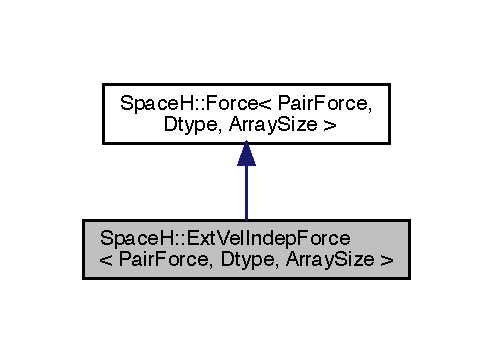
\includegraphics[width=237pt]{struct_space_h_1_1_ext_vel_indep_force__inherit__graph}
\end{center}
\end{figure}


Collaboration diagram for SpaceH\+:\+:Ext\+Vel\+Indep\+Force$<$ Ext\+Force, Dtype, Array\+Size $>$\+:\nopagebreak
\begin{figure}[H]
\begin{center}
\leavevmode
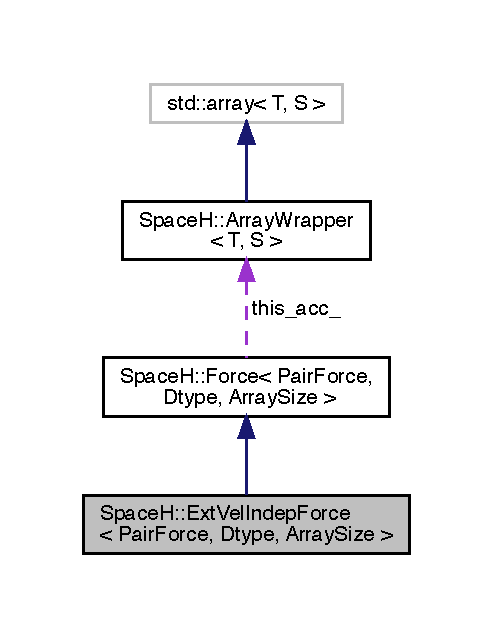
\includegraphics[width=237pt]{struct_space_h_1_1_ext_vel_indep_force__coll__graph}
\end{center}
\end{figure}
\subsection*{Public Types}
\begin{DoxyCompactItemize}
\item 
using \mbox{\hyperlink{struct_space_h_1_1_ext_vel_indep_force_acf786913cd012bc90bb02f9ae1f87e91}{Base}} = \mbox{\hyperlink{struct_space_h_1_1_force}{Force}}$<$ Ext\+Force, Dtype, Array\+Size $>$
\item 
using \mbox{\hyperlink{struct_space_h_1_1_ext_vel_indep_force_a6db7150bace18b57cb059989c7f29e50}{type}} = typename \mbox{\hyperlink{struct_space_h_1_1_force_a151c6ae1ec7ad87825c2b6cc74aee5f2}{Base\+::type}}
\item 
using \mbox{\hyperlink{struct_space_h_1_1_ext_vel_indep_force_afe9c9f6c747f7b82f5e1058f5df2f2af}{Scalar\+Array}} = typename type\+::\+Scalar\+Array
\item 
using \mbox{\hyperlink{struct_space_h_1_1_ext_vel_indep_force_ae9d2ecd856cbcfa1cc848003a8450adf}{Vector\+Array}} = typename type\+::\+Vector\+Array
\end{DoxyCompactItemize}
\subsection*{Public Member Functions}
\begin{DoxyCompactItemize}
\item 
void \mbox{\hyperlink{struct_space_h_1_1_ext_vel_indep_force_ade2a9eececdb0833213048c1e73c7756}{calcu\+Acc}} (const \mbox{\hyperlink{struct_space_h_1_1_ext_vel_indep_force_afe9c9f6c747f7b82f5e1058f5df2f2af}{Scalar\+Array}} \&mass, const \mbox{\hyperlink{struct_space_h_1_1_ext_vel_indep_force_ae9d2ecd856cbcfa1cc848003a8450adf}{Vector\+Array}} \&pos)
\end{DoxyCompactItemize}
\subsection*{Additional Inherited Members}


\subsection{Member Typedef Documentation}
\mbox{\Hypertarget{struct_space_h_1_1_ext_vel_indep_force_acf786913cd012bc90bb02f9ae1f87e91}\label{struct_space_h_1_1_ext_vel_indep_force_acf786913cd012bc90bb02f9ae1f87e91}} 
\index{Space\+H\+::\+Ext\+Vel\+Indep\+Force@{Space\+H\+::\+Ext\+Vel\+Indep\+Force}!Base@{Base}}
\index{Base@{Base}!Space\+H\+::\+Ext\+Vel\+Indep\+Force@{Space\+H\+::\+Ext\+Vel\+Indep\+Force}}
\subsubsection{\texorpdfstring{Base}{Base}}
{\footnotesize\ttfamily template$<$typename Ext\+Force, typename Dtype, size\+\_\+t Array\+Size$>$ \\
using \mbox{\hyperlink{struct_space_h_1_1_ext_vel_indep_force}{Space\+H\+::\+Ext\+Vel\+Indep\+Force}}$<$ Ext\+Force, Dtype, Array\+Size $>$\+::\mbox{\hyperlink{struct_space_h_1_1_ext_vel_indep_force_acf786913cd012bc90bb02f9ae1f87e91}{Base}} =  \mbox{\hyperlink{struct_space_h_1_1_force}{Force}}$<$Ext\+Force, Dtype, Array\+Size$>$}

\mbox{\Hypertarget{struct_space_h_1_1_ext_vel_indep_force_afe9c9f6c747f7b82f5e1058f5df2f2af}\label{struct_space_h_1_1_ext_vel_indep_force_afe9c9f6c747f7b82f5e1058f5df2f2af}} 
\index{Space\+H\+::\+Ext\+Vel\+Indep\+Force@{Space\+H\+::\+Ext\+Vel\+Indep\+Force}!Scalar\+Array@{Scalar\+Array}}
\index{Scalar\+Array@{Scalar\+Array}!Space\+H\+::\+Ext\+Vel\+Indep\+Force@{Space\+H\+::\+Ext\+Vel\+Indep\+Force}}
\subsubsection{\texorpdfstring{Scalar\+Array}{ScalarArray}}
{\footnotesize\ttfamily template$<$typename Ext\+Force, typename Dtype, size\+\_\+t Array\+Size$>$ \\
using \mbox{\hyperlink{struct_space_h_1_1_ext_vel_indep_force}{Space\+H\+::\+Ext\+Vel\+Indep\+Force}}$<$ Ext\+Force, Dtype, Array\+Size $>$\+::\mbox{\hyperlink{struct_space_h_1_1_ext_vel_indep_force_afe9c9f6c747f7b82f5e1058f5df2f2af}{Scalar\+Array}} =  typename type\+::\+Scalar\+Array}

\mbox{\Hypertarget{struct_space_h_1_1_ext_vel_indep_force_a6db7150bace18b57cb059989c7f29e50}\label{struct_space_h_1_1_ext_vel_indep_force_a6db7150bace18b57cb059989c7f29e50}} 
\index{Space\+H\+::\+Ext\+Vel\+Indep\+Force@{Space\+H\+::\+Ext\+Vel\+Indep\+Force}!type@{type}}
\index{type@{type}!Space\+H\+::\+Ext\+Vel\+Indep\+Force@{Space\+H\+::\+Ext\+Vel\+Indep\+Force}}
\subsubsection{\texorpdfstring{type}{type}}
{\footnotesize\ttfamily template$<$typename Ext\+Force, typename Dtype, size\+\_\+t Array\+Size$>$ \\
using \mbox{\hyperlink{struct_space_h_1_1_ext_vel_indep_force}{Space\+H\+::\+Ext\+Vel\+Indep\+Force}}$<$ Ext\+Force, Dtype, Array\+Size $>$\+::\mbox{\hyperlink{struct_space_h_1_1_ext_vel_indep_force_a6db7150bace18b57cb059989c7f29e50}{type}} =  typename \mbox{\hyperlink{struct_space_h_1_1_force_a151c6ae1ec7ad87825c2b6cc74aee5f2}{Base\+::type}}}

\mbox{\Hypertarget{struct_space_h_1_1_ext_vel_indep_force_ae9d2ecd856cbcfa1cc848003a8450adf}\label{struct_space_h_1_1_ext_vel_indep_force_ae9d2ecd856cbcfa1cc848003a8450adf}} 
\index{Space\+H\+::\+Ext\+Vel\+Indep\+Force@{Space\+H\+::\+Ext\+Vel\+Indep\+Force}!Vector\+Array@{Vector\+Array}}
\index{Vector\+Array@{Vector\+Array}!Space\+H\+::\+Ext\+Vel\+Indep\+Force@{Space\+H\+::\+Ext\+Vel\+Indep\+Force}}
\subsubsection{\texorpdfstring{Vector\+Array}{VectorArray}}
{\footnotesize\ttfamily template$<$typename Ext\+Force, typename Dtype, size\+\_\+t Array\+Size$>$ \\
using \mbox{\hyperlink{struct_space_h_1_1_ext_vel_indep_force}{Space\+H\+::\+Ext\+Vel\+Indep\+Force}}$<$ Ext\+Force, Dtype, Array\+Size $>$\+::\mbox{\hyperlink{struct_space_h_1_1_ext_vel_indep_force_ae9d2ecd856cbcfa1cc848003a8450adf}{Vector\+Array}} =  typename type\+::\+Vector\+Array}



\subsection{Member Function Documentation}
\mbox{\Hypertarget{struct_space_h_1_1_ext_vel_indep_force_ade2a9eececdb0833213048c1e73c7756}\label{struct_space_h_1_1_ext_vel_indep_force_ade2a9eececdb0833213048c1e73c7756}} 
\index{Space\+H\+::\+Ext\+Vel\+Indep\+Force@{Space\+H\+::\+Ext\+Vel\+Indep\+Force}!calcu\+Acc@{calcu\+Acc}}
\index{calcu\+Acc@{calcu\+Acc}!Space\+H\+::\+Ext\+Vel\+Indep\+Force@{Space\+H\+::\+Ext\+Vel\+Indep\+Force}}
\subsubsection{\texorpdfstring{calcu\+Acc()}{calcuAcc()}}
{\footnotesize\ttfamily template$<$typename Ext\+Force, typename Dtype, size\+\_\+t Array\+Size$>$ \\
void \mbox{\hyperlink{struct_space_h_1_1_ext_vel_indep_force}{Space\+H\+::\+Ext\+Vel\+Indep\+Force}}$<$ Ext\+Force, Dtype, Array\+Size $>$\+::calcu\+Acc (\begin{DoxyParamCaption}\item[{const \mbox{\hyperlink{struct_space_h_1_1_ext_vel_indep_force_afe9c9f6c747f7b82f5e1058f5df2f2af}{Scalar\+Array}} \&}]{mass,  }\item[{const \mbox{\hyperlink{struct_space_h_1_1_ext_vel_indep_force_ae9d2ecd856cbcfa1cc848003a8450adf}{Vector\+Array}} \&}]{pos }\end{DoxyParamCaption})\hspace{0.3cm}{\ttfamily [inline]}}

Here is the caller graph for this function\+:
\nopagebreak
\begin{figure}[H]
\begin{center}
\leavevmode
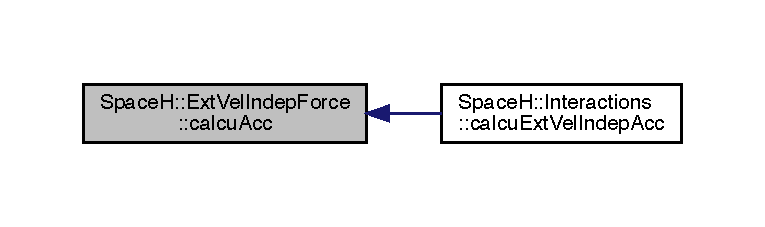
\includegraphics[width=350pt]{struct_space_h_1_1_ext_vel_indep_force_ade2a9eececdb0833213048c1e73c7756_icgraph}
\end{center}
\end{figure}


The documentation for this struct was generated from the following file\+:\begin{DoxyCompactItemize}
\item 
interaction/\mbox{\hyperlink{force_8h}{force.\+h}}\end{DoxyCompactItemize}

\hypertarget{struct_space_h_1_1_ext_vel_indep_force_3_01void_00_01_dtype_00_01_array_size_01_4}{}\section{SpaceH\+:\+:Ext\+Vel\+Indep\+Force$<$ void, Dtype, Array\+Size $>$ Struct Template Reference}
\label{struct_space_h_1_1_ext_vel_indep_force_3_01void_00_01_dtype_00_01_array_size_01_4}\index{Space\+H\+::\+Ext\+Vel\+Indep\+Force$<$ void, Dtype, Array\+Size $>$@{Space\+H\+::\+Ext\+Vel\+Indep\+Force$<$ void, Dtype, Array\+Size $>$}}


{\ttfamily \#include $<$force.\+h$>$}

\subsection*{Public Types}
\begin{DoxyCompactItemize}
\item 
using \mbox{\hyperlink{struct_space_h_1_1_ext_vel_indep_force_3_01void_00_01_dtype_00_01_array_size_01_4_a1d5ec14368fdd57d1cea251229ba72f7}{type}} = \mbox{\hyperlink{struct_space_h_1_1_proto_type}{Space\+H\+::\+Proto\+Type}}$<$ Dtype, Array\+Size $>$
\item 
using \mbox{\hyperlink{struct_space_h_1_1_ext_vel_indep_force_3_01void_00_01_dtype_00_01_array_size_01_4_ab186d960b853d69afb7cdbb19af71639}{Scalar\+Array}} = typename \mbox{\hyperlink{struct_space_h_1_1_proto_type_a09ef91dc8a37a044c403f5a833044725}{type\+::\+Scalar\+Array}}
\item 
using \mbox{\hyperlink{struct_space_h_1_1_ext_vel_indep_force_3_01void_00_01_dtype_00_01_array_size_01_4_a2f23924c3395826cf1701b5b0c74be50}{Vector\+Array}} = typename \mbox{\hyperlink{struct_space_h_1_1_proto_type_a622b8e122b33bb4966a02299fb7b82d6}{type\+::\+Vector\+Array}}
\end{DoxyCompactItemize}
\subsection*{Public Member Functions}
\begin{DoxyCompactItemize}
\item 
void \mbox{\hyperlink{struct_space_h_1_1_ext_vel_indep_force_3_01void_00_01_dtype_00_01_array_size_01_4_a358d0f758147a31d7d9e41b8e4d7fda7}{add\+Total}} (\mbox{\hyperlink{struct_space_h_1_1_ext_vel_indep_force_3_01void_00_01_dtype_00_01_array_size_01_4_a2f23924c3395826cf1701b5b0c74be50}{Vector\+Array}} \&acc)
\item 
void \mbox{\hyperlink{struct_space_h_1_1_ext_vel_indep_force_3_01void_00_01_dtype_00_01_array_size_01_4_a2eaf0655966479362ded7fddc5273008}{calcu\+Acc}} (const \mbox{\hyperlink{struct_space_h_1_1_ext_vel_indep_force_3_01void_00_01_dtype_00_01_array_size_01_4_ab186d960b853d69afb7cdbb19af71639}{Scalar\+Array}} \&mass, const \mbox{\hyperlink{struct_space_h_1_1_ext_vel_indep_force_3_01void_00_01_dtype_00_01_array_size_01_4_a2f23924c3395826cf1701b5b0c74be50}{Vector\+Array}} \&pos)
\end{DoxyCompactItemize}


\subsection{Member Typedef Documentation}
\mbox{\Hypertarget{struct_space_h_1_1_ext_vel_indep_force_3_01void_00_01_dtype_00_01_array_size_01_4_ab186d960b853d69afb7cdbb19af71639}\label{struct_space_h_1_1_ext_vel_indep_force_3_01void_00_01_dtype_00_01_array_size_01_4_ab186d960b853d69afb7cdbb19af71639}} 
\index{Space\+H\+::\+Ext\+Vel\+Indep\+Force$<$ void, Dtype, Array\+Size $>$@{Space\+H\+::\+Ext\+Vel\+Indep\+Force$<$ void, Dtype, Array\+Size $>$}!Scalar\+Array@{Scalar\+Array}}
\index{Scalar\+Array@{Scalar\+Array}!Space\+H\+::\+Ext\+Vel\+Indep\+Force$<$ void, Dtype, Array\+Size $>$@{Space\+H\+::\+Ext\+Vel\+Indep\+Force$<$ void, Dtype, Array\+Size $>$}}
\subsubsection{\texorpdfstring{Scalar\+Array}{ScalarArray}}
{\footnotesize\ttfamily template$<$typename Dtype , size\+\_\+t Array\+Size$>$ \\
using \mbox{\hyperlink{struct_space_h_1_1_ext_vel_indep_force}{Space\+H\+::\+Ext\+Vel\+Indep\+Force}}$<$ void, Dtype, Array\+Size $>$\+::\mbox{\hyperlink{struct_space_h_1_1_ext_vel_indep_force_3_01void_00_01_dtype_00_01_array_size_01_4_ab186d960b853d69afb7cdbb19af71639}{Scalar\+Array}} =  typename \mbox{\hyperlink{struct_space_h_1_1_proto_type_a09ef91dc8a37a044c403f5a833044725}{type\+::\+Scalar\+Array}}}

\mbox{\Hypertarget{struct_space_h_1_1_ext_vel_indep_force_3_01void_00_01_dtype_00_01_array_size_01_4_a1d5ec14368fdd57d1cea251229ba72f7}\label{struct_space_h_1_1_ext_vel_indep_force_3_01void_00_01_dtype_00_01_array_size_01_4_a1d5ec14368fdd57d1cea251229ba72f7}} 
\index{Space\+H\+::\+Ext\+Vel\+Indep\+Force$<$ void, Dtype, Array\+Size $>$@{Space\+H\+::\+Ext\+Vel\+Indep\+Force$<$ void, Dtype, Array\+Size $>$}!type@{type}}
\index{type@{type}!Space\+H\+::\+Ext\+Vel\+Indep\+Force$<$ void, Dtype, Array\+Size $>$@{Space\+H\+::\+Ext\+Vel\+Indep\+Force$<$ void, Dtype, Array\+Size $>$}}
\subsubsection{\texorpdfstring{type}{type}}
{\footnotesize\ttfamily template$<$typename Dtype , size\+\_\+t Array\+Size$>$ \\
using \mbox{\hyperlink{struct_space_h_1_1_ext_vel_indep_force}{Space\+H\+::\+Ext\+Vel\+Indep\+Force}}$<$ void, Dtype, Array\+Size $>$\+::\mbox{\hyperlink{struct_space_h_1_1_ext_vel_indep_force_3_01void_00_01_dtype_00_01_array_size_01_4_a1d5ec14368fdd57d1cea251229ba72f7}{type}} =  \mbox{\hyperlink{struct_space_h_1_1_proto_type}{Space\+H\+::\+Proto\+Type}}$<$Dtype, Array\+Size$>$}

\mbox{\Hypertarget{struct_space_h_1_1_ext_vel_indep_force_3_01void_00_01_dtype_00_01_array_size_01_4_a2f23924c3395826cf1701b5b0c74be50}\label{struct_space_h_1_1_ext_vel_indep_force_3_01void_00_01_dtype_00_01_array_size_01_4_a2f23924c3395826cf1701b5b0c74be50}} 
\index{Space\+H\+::\+Ext\+Vel\+Indep\+Force$<$ void, Dtype, Array\+Size $>$@{Space\+H\+::\+Ext\+Vel\+Indep\+Force$<$ void, Dtype, Array\+Size $>$}!Vector\+Array@{Vector\+Array}}
\index{Vector\+Array@{Vector\+Array}!Space\+H\+::\+Ext\+Vel\+Indep\+Force$<$ void, Dtype, Array\+Size $>$@{Space\+H\+::\+Ext\+Vel\+Indep\+Force$<$ void, Dtype, Array\+Size $>$}}
\subsubsection{\texorpdfstring{Vector\+Array}{VectorArray}}
{\footnotesize\ttfamily template$<$typename Dtype , size\+\_\+t Array\+Size$>$ \\
using \mbox{\hyperlink{struct_space_h_1_1_ext_vel_indep_force}{Space\+H\+::\+Ext\+Vel\+Indep\+Force}}$<$ void, Dtype, Array\+Size $>$\+::\mbox{\hyperlink{struct_space_h_1_1_ext_vel_indep_force_3_01void_00_01_dtype_00_01_array_size_01_4_a2f23924c3395826cf1701b5b0c74be50}{Vector\+Array}} =  typename \mbox{\hyperlink{struct_space_h_1_1_proto_type_a622b8e122b33bb4966a02299fb7b82d6}{type\+::\+Vector\+Array}}}



\subsection{Member Function Documentation}
\mbox{\Hypertarget{struct_space_h_1_1_ext_vel_indep_force_3_01void_00_01_dtype_00_01_array_size_01_4_a358d0f758147a31d7d9e41b8e4d7fda7}\label{struct_space_h_1_1_ext_vel_indep_force_3_01void_00_01_dtype_00_01_array_size_01_4_a358d0f758147a31d7d9e41b8e4d7fda7}} 
\index{Space\+H\+::\+Ext\+Vel\+Indep\+Force$<$ void, Dtype, Array\+Size $>$@{Space\+H\+::\+Ext\+Vel\+Indep\+Force$<$ void, Dtype, Array\+Size $>$}!add\+Total@{add\+Total}}
\index{add\+Total@{add\+Total}!Space\+H\+::\+Ext\+Vel\+Indep\+Force$<$ void, Dtype, Array\+Size $>$@{Space\+H\+::\+Ext\+Vel\+Indep\+Force$<$ void, Dtype, Array\+Size $>$}}
\subsubsection{\texorpdfstring{add\+Total()}{addTotal()}}
{\footnotesize\ttfamily template$<$typename Dtype , size\+\_\+t Array\+Size$>$ \\
void \mbox{\hyperlink{struct_space_h_1_1_ext_vel_indep_force}{Space\+H\+::\+Ext\+Vel\+Indep\+Force}}$<$ void, Dtype, Array\+Size $>$\+::add\+Total (\begin{DoxyParamCaption}\item[{\mbox{\hyperlink{struct_space_h_1_1_ext_vel_indep_force_3_01void_00_01_dtype_00_01_array_size_01_4_a2f23924c3395826cf1701b5b0c74be50}{Vector\+Array}} \&}]{acc }\end{DoxyParamCaption})\hspace{0.3cm}{\ttfamily [inline]}}

\mbox{\Hypertarget{struct_space_h_1_1_ext_vel_indep_force_3_01void_00_01_dtype_00_01_array_size_01_4_a2eaf0655966479362ded7fddc5273008}\label{struct_space_h_1_1_ext_vel_indep_force_3_01void_00_01_dtype_00_01_array_size_01_4_a2eaf0655966479362ded7fddc5273008}} 
\index{Space\+H\+::\+Ext\+Vel\+Indep\+Force$<$ void, Dtype, Array\+Size $>$@{Space\+H\+::\+Ext\+Vel\+Indep\+Force$<$ void, Dtype, Array\+Size $>$}!calcu\+Acc@{calcu\+Acc}}
\index{calcu\+Acc@{calcu\+Acc}!Space\+H\+::\+Ext\+Vel\+Indep\+Force$<$ void, Dtype, Array\+Size $>$@{Space\+H\+::\+Ext\+Vel\+Indep\+Force$<$ void, Dtype, Array\+Size $>$}}
\subsubsection{\texorpdfstring{calcu\+Acc()}{calcuAcc()}}
{\footnotesize\ttfamily template$<$typename Dtype , size\+\_\+t Array\+Size$>$ \\
void \mbox{\hyperlink{struct_space_h_1_1_ext_vel_indep_force}{Space\+H\+::\+Ext\+Vel\+Indep\+Force}}$<$ void, Dtype, Array\+Size $>$\+::calcu\+Acc (\begin{DoxyParamCaption}\item[{const \mbox{\hyperlink{struct_space_h_1_1_ext_vel_indep_force_3_01void_00_01_dtype_00_01_array_size_01_4_ab186d960b853d69afb7cdbb19af71639}{Scalar\+Array}} \&}]{mass,  }\item[{const \mbox{\hyperlink{struct_space_h_1_1_ext_vel_indep_force_3_01void_00_01_dtype_00_01_array_size_01_4_a2f23924c3395826cf1701b5b0c74be50}{Vector\+Array}} \&}]{pos }\end{DoxyParamCaption})\hspace{0.3cm}{\ttfamily [inline]}}



The documentation for this struct was generated from the following file\+:\begin{DoxyCompactItemize}
\item 
interaction/\mbox{\hyperlink{force_8h}{force.\+h}}\end{DoxyCompactItemize}

\hypertarget{struct_space_h_1_1_force}{}\section{SpaceH\+:\+:Force$<$ Forcefunc, Dtype, Array\+Size $>$ Struct Template Reference}
\label{struct_space_h_1_1_force}\index{Space\+H\+::\+Force$<$ Forcefunc, Dtype, Array\+Size $>$@{Space\+H\+::\+Force$<$ Forcefunc, Dtype, Array\+Size $>$}}


{\ttfamily \#include $<$force.\+h$>$}



Collaboration diagram for SpaceH\+:\+:Force$<$ Forcefunc, Dtype, Array\+Size $>$\+:\nopagebreak
\begin{figure}[H]
\begin{center}
\leavevmode
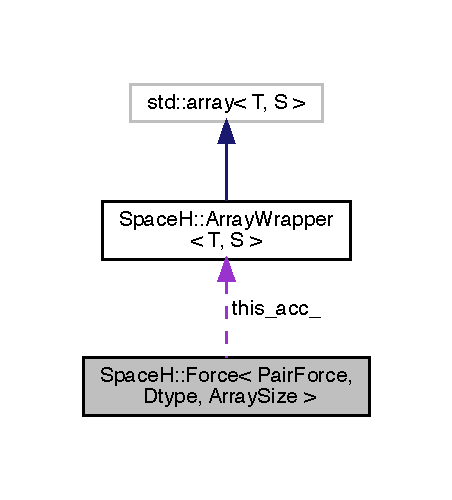
\includegraphics[width=217pt]{struct_space_h_1_1_force__coll__graph}
\end{center}
\end{figure}
\subsection*{Public Types}
\begin{DoxyCompactItemize}
\item 
using \mbox{\hyperlink{struct_space_h_1_1_force_a151c6ae1ec7ad87825c2b6cc74aee5f2}{type}} = \mbox{\hyperlink{struct_space_h_1_1_proto_type}{Space\+H\+::\+Proto\+Type}}$<$ Dtype, Array\+Size $>$
\item 
using \mbox{\hyperlink{struct_space_h_1_1_force_a7da326c7793f559bb39c73b6d0d01e39}{Vector}} = typename \mbox{\hyperlink{struct_space_h_1_1_proto_type_a316b81f4660b2b4fab14a8e1f23b6089}{type\+::\+Vector}}
\item 
using \mbox{\hyperlink{struct_space_h_1_1_force_aa58fd21903006c1d033713d04b4719f3}{Vector\+Array}} = typename \mbox{\hyperlink{struct_space_h_1_1_proto_type_a622b8e122b33bb4966a02299fb7b82d6}{type\+::\+Vector\+Array}}
\end{DoxyCompactItemize}
\subsection*{Public Member Functions}
\begin{DoxyCompactItemize}
\item 
void \mbox{\hyperlink{struct_space_h_1_1_force_a9f85a2d5e3e642c6e1121c591c19dded}{add\+Total}} (\mbox{\hyperlink{struct_space_h_1_1_force_aa58fd21903006c1d033713d04b4719f3}{Vector\+Array}} \&\mbox{\hyperlink{struct_space_h_1_1_force_ac4f8ce97d4513859ad94064ed35ab300}{acc}})
\item 
const \mbox{\hyperlink{struct_space_h_1_1_force_aa58fd21903006c1d033713d04b4719f3}{Vector\+Array}} \& \mbox{\hyperlink{struct_space_h_1_1_force_ac4f8ce97d4513859ad94064ed35ab300}{acc}} () const
\item 
const \mbox{\hyperlink{struct_space_h_1_1_force_a7da326c7793f559bb39c73b6d0d01e39}{Vector}} \& \mbox{\hyperlink{struct_space_h_1_1_force_abff837e46b01461762054d79ebee0fb8}{acc}} (size\+\_\+t i) const
\item 
void \mbox{\hyperlink{struct_space_h_1_1_force_aa1a3ef23a57eb72d0004c4afe505eb0b}{check\+Array\+Size}} (size\+\_\+t size)
\end{DoxyCompactItemize}
\subsection*{Protected Attributes}
\begin{DoxyCompactItemize}
\item 
\mbox{\hyperlink{struct_space_h_1_1_force_aa58fd21903006c1d033713d04b4719f3}{Vector\+Array}} \mbox{\hyperlink{struct_space_h_1_1_force_a7e87abc40a345bc5e24bdf56ca32f045}{this\+\_\+acc\+\_\+}}
\item 
Forcefunc \mbox{\hyperlink{struct_space_h_1_1_force_a9d669e983d78f8bfa0e1a08dd27b6abb}{force\+\_\+}}
\end{DoxyCompactItemize}


\subsection{Member Typedef Documentation}
\mbox{\Hypertarget{struct_space_h_1_1_force_a151c6ae1ec7ad87825c2b6cc74aee5f2}\label{struct_space_h_1_1_force_a151c6ae1ec7ad87825c2b6cc74aee5f2}} 
\index{Space\+H\+::\+Force@{Space\+H\+::\+Force}!type@{type}}
\index{type@{type}!Space\+H\+::\+Force@{Space\+H\+::\+Force}}
\subsubsection{\texorpdfstring{type}{type}}
{\footnotesize\ttfamily template$<$typename Forcefunc, typename Dtype, size\+\_\+t Array\+Size$>$ \\
using \mbox{\hyperlink{struct_space_h_1_1_force}{Space\+H\+::\+Force}}$<$ Forcefunc, Dtype, Array\+Size $>$\+::\mbox{\hyperlink{struct_space_h_1_1_force_a151c6ae1ec7ad87825c2b6cc74aee5f2}{type}} =  \mbox{\hyperlink{struct_space_h_1_1_proto_type}{Space\+H\+::\+Proto\+Type}}$<$Dtype, Array\+Size$>$}

\mbox{\Hypertarget{struct_space_h_1_1_force_a7da326c7793f559bb39c73b6d0d01e39}\label{struct_space_h_1_1_force_a7da326c7793f559bb39c73b6d0d01e39}} 
\index{Space\+H\+::\+Force@{Space\+H\+::\+Force}!Vector@{Vector}}
\index{Vector@{Vector}!Space\+H\+::\+Force@{Space\+H\+::\+Force}}
\subsubsection{\texorpdfstring{Vector}{Vector}}
{\footnotesize\ttfamily template$<$typename Forcefunc, typename Dtype, size\+\_\+t Array\+Size$>$ \\
using \mbox{\hyperlink{struct_space_h_1_1_force}{Space\+H\+::\+Force}}$<$ Forcefunc, Dtype, Array\+Size $>$\+::\mbox{\hyperlink{struct_space_h_1_1_force_a7da326c7793f559bb39c73b6d0d01e39}{Vector}} =  typename \mbox{\hyperlink{struct_space_h_1_1_proto_type_a316b81f4660b2b4fab14a8e1f23b6089}{type\+::\+Vector}}}

\mbox{\Hypertarget{struct_space_h_1_1_force_aa58fd21903006c1d033713d04b4719f3}\label{struct_space_h_1_1_force_aa58fd21903006c1d033713d04b4719f3}} 
\index{Space\+H\+::\+Force@{Space\+H\+::\+Force}!Vector\+Array@{Vector\+Array}}
\index{Vector\+Array@{Vector\+Array}!Space\+H\+::\+Force@{Space\+H\+::\+Force}}
\subsubsection{\texorpdfstring{Vector\+Array}{VectorArray}}
{\footnotesize\ttfamily template$<$typename Forcefunc, typename Dtype, size\+\_\+t Array\+Size$>$ \\
using \mbox{\hyperlink{struct_space_h_1_1_force}{Space\+H\+::\+Force}}$<$ Forcefunc, Dtype, Array\+Size $>$\+::\mbox{\hyperlink{struct_space_h_1_1_force_aa58fd21903006c1d033713d04b4719f3}{Vector\+Array}} =  typename \mbox{\hyperlink{struct_space_h_1_1_proto_type_a622b8e122b33bb4966a02299fb7b82d6}{type\+::\+Vector\+Array}}}



\subsection{Member Function Documentation}
\mbox{\Hypertarget{struct_space_h_1_1_force_ac4f8ce97d4513859ad94064ed35ab300}\label{struct_space_h_1_1_force_ac4f8ce97d4513859ad94064ed35ab300}} 
\index{Space\+H\+::\+Force@{Space\+H\+::\+Force}!acc@{acc}}
\index{acc@{acc}!Space\+H\+::\+Force@{Space\+H\+::\+Force}}
\subsubsection{\texorpdfstring{acc()}{acc()}\hspace{0.1cm}{\footnotesize\ttfamily [1/2]}}
{\footnotesize\ttfamily template$<$typename Forcefunc, typename Dtype, size\+\_\+t Array\+Size$>$ \\
const \mbox{\hyperlink{struct_space_h_1_1_force_aa58fd21903006c1d033713d04b4719f3}{Vector\+Array}}\& \mbox{\hyperlink{struct_space_h_1_1_force}{Space\+H\+::\+Force}}$<$ Forcefunc, Dtype, Array\+Size $>$\+::acc (\begin{DoxyParamCaption}{ }\end{DoxyParamCaption}) const\hspace{0.3cm}{\ttfamily [inline]}}

Here is the caller graph for this function\+:
\nopagebreak
\begin{figure}[H]
\begin{center}
\leavevmode
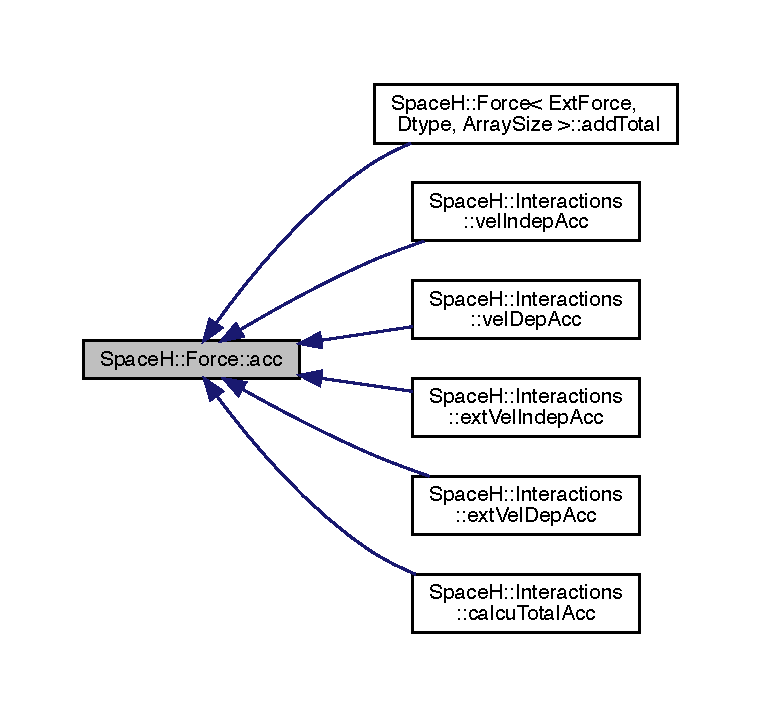
\includegraphics[width=350pt]{struct_space_h_1_1_force_ac4f8ce97d4513859ad94064ed35ab300_icgraph}
\end{center}
\end{figure}
\mbox{\Hypertarget{struct_space_h_1_1_force_abff837e46b01461762054d79ebee0fb8}\label{struct_space_h_1_1_force_abff837e46b01461762054d79ebee0fb8}} 
\index{Space\+H\+::\+Force@{Space\+H\+::\+Force}!acc@{acc}}
\index{acc@{acc}!Space\+H\+::\+Force@{Space\+H\+::\+Force}}
\subsubsection{\texorpdfstring{acc()}{acc()}\hspace{0.1cm}{\footnotesize\ttfamily [2/2]}}
{\footnotesize\ttfamily template$<$typename Forcefunc, typename Dtype, size\+\_\+t Array\+Size$>$ \\
const \mbox{\hyperlink{struct_space_h_1_1_force_a7da326c7793f559bb39c73b6d0d01e39}{Vector}}\& \mbox{\hyperlink{struct_space_h_1_1_force}{Space\+H\+::\+Force}}$<$ Forcefunc, Dtype, Array\+Size $>$\+::acc (\begin{DoxyParamCaption}\item[{size\+\_\+t}]{i }\end{DoxyParamCaption}) const\hspace{0.3cm}{\ttfamily [inline]}}

\mbox{\Hypertarget{struct_space_h_1_1_force_a9f85a2d5e3e642c6e1121c591c19dded}\label{struct_space_h_1_1_force_a9f85a2d5e3e642c6e1121c591c19dded}} 
\index{Space\+H\+::\+Force@{Space\+H\+::\+Force}!add\+Total@{add\+Total}}
\index{add\+Total@{add\+Total}!Space\+H\+::\+Force@{Space\+H\+::\+Force}}
\subsubsection{\texorpdfstring{add\+Total()}{addTotal()}}
{\footnotesize\ttfamily template$<$typename Forcefunc, typename Dtype, size\+\_\+t Array\+Size$>$ \\
void \mbox{\hyperlink{struct_space_h_1_1_force}{Space\+H\+::\+Force}}$<$ Forcefunc, Dtype, Array\+Size $>$\+::add\+Total (\begin{DoxyParamCaption}\item[{\mbox{\hyperlink{struct_space_h_1_1_force_aa58fd21903006c1d033713d04b4719f3}{Vector\+Array}} \&}]{acc }\end{DoxyParamCaption})\hspace{0.3cm}{\ttfamily [inline]}}

Here is the caller graph for this function\+:
\nopagebreak
\begin{figure}[H]
\begin{center}
\leavevmode
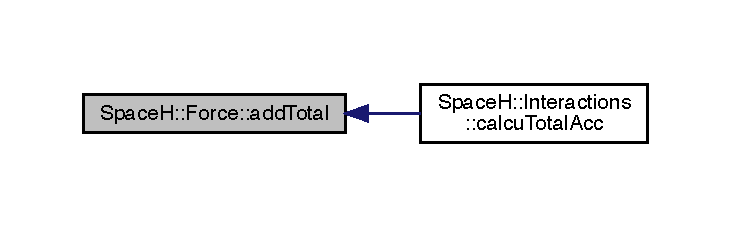
\includegraphics[width=350pt]{struct_space_h_1_1_force_a9f85a2d5e3e642c6e1121c591c19dded_icgraph}
\end{center}
\end{figure}
\mbox{\Hypertarget{struct_space_h_1_1_force_aa1a3ef23a57eb72d0004c4afe505eb0b}\label{struct_space_h_1_1_force_aa1a3ef23a57eb72d0004c4afe505eb0b}} 
\index{Space\+H\+::\+Force@{Space\+H\+::\+Force}!check\+Array\+Size@{check\+Array\+Size}}
\index{check\+Array\+Size@{check\+Array\+Size}!Space\+H\+::\+Force@{Space\+H\+::\+Force}}
\subsubsection{\texorpdfstring{check\+Array\+Size()}{checkArraySize()}}
{\footnotesize\ttfamily template$<$typename Forcefunc, typename Dtype, size\+\_\+t Array\+Size$>$ \\
void \mbox{\hyperlink{struct_space_h_1_1_force}{Space\+H\+::\+Force}}$<$ Forcefunc, Dtype, Array\+Size $>$\+::check\+Array\+Size (\begin{DoxyParamCaption}\item[{size\+\_\+t}]{size }\end{DoxyParamCaption})\hspace{0.3cm}{\ttfamily [inline]}}



\subsection{Member Data Documentation}
\mbox{\Hypertarget{struct_space_h_1_1_force_a9d669e983d78f8bfa0e1a08dd27b6abb}\label{struct_space_h_1_1_force_a9d669e983d78f8bfa0e1a08dd27b6abb}} 
\index{Space\+H\+::\+Force@{Space\+H\+::\+Force}!force\+\_\+@{force\+\_\+}}
\index{force\+\_\+@{force\+\_\+}!Space\+H\+::\+Force@{Space\+H\+::\+Force}}
\subsubsection{\texorpdfstring{force\+\_\+}{force\_}}
{\footnotesize\ttfamily template$<$typename Forcefunc, typename Dtype, size\+\_\+t Array\+Size$>$ \\
Forcefunc \mbox{\hyperlink{struct_space_h_1_1_force}{Space\+H\+::\+Force}}$<$ Forcefunc, Dtype, Array\+Size $>$\+::force\+\_\+\hspace{0.3cm}{\ttfamily [protected]}}

\mbox{\Hypertarget{struct_space_h_1_1_force_a7e87abc40a345bc5e24bdf56ca32f045}\label{struct_space_h_1_1_force_a7e87abc40a345bc5e24bdf56ca32f045}} 
\index{Space\+H\+::\+Force@{Space\+H\+::\+Force}!this\+\_\+acc\+\_\+@{this\+\_\+acc\+\_\+}}
\index{this\+\_\+acc\+\_\+@{this\+\_\+acc\+\_\+}!Space\+H\+::\+Force@{Space\+H\+::\+Force}}
\subsubsection{\texorpdfstring{this\+\_\+acc\+\_\+}{this\_acc\_}}
{\footnotesize\ttfamily template$<$typename Forcefunc, typename Dtype, size\+\_\+t Array\+Size$>$ \\
\mbox{\hyperlink{struct_space_h_1_1_force_aa58fd21903006c1d033713d04b4719f3}{Vector\+Array}} \mbox{\hyperlink{struct_space_h_1_1_force}{Space\+H\+::\+Force}}$<$ Forcefunc, Dtype, Array\+Size $>$\+::this\+\_\+acc\+\_\+\hspace{0.3cm}{\ttfamily [protected]}}



The documentation for this struct was generated from the following file\+:\begin{DoxyCompactItemize}
\item 
interaction/\mbox{\hyperlink{force_8h}{force.\+h}}\end{DoxyCompactItemize}

\hypertarget{class_space_h_1_1_gauss_dadau}{}\section{SpaceH\+:\+:Gauss\+Dadau$<$ Partic\+Sys $>$ Class Template Reference}
\label{class_space_h_1_1_gauss_dadau}\index{Space\+H\+::\+Gauss\+Dadau$<$ Partic\+Sys $>$@{Space\+H\+::\+Gauss\+Dadau$<$ Partic\+Sys $>$}}


Gauss-\/\+Dadau integrator.  




{\ttfamily \#include $<$Gauss-\/\+Dadau.\+h$>$}

\subsection*{Public Types}
\begin{DoxyCompactItemize}
\item 
using \mbox{\hyperlink{class_space_h_1_1_gauss_dadau_a780629d19a82feeab959cd68c8a5f8a3}{type}} = typename Partic\+Sys\+::type
\item 
using \mbox{\hyperlink{class_space_h_1_1_gauss_dadau_ace42540e9fb47d7f1d1f00622bbd1ccb}{Scalar}} = typename type\+::\+Scalar
\item 
using \mbox{\hyperlink{class_space_h_1_1_gauss_dadau_a2019bc4c1ee812f59a32f9273c84f5be}{Vector}} = typename type\+::\+Vector
\item 
using \mbox{\hyperlink{class_space_h_1_1_gauss_dadau_a69e00c49f96f4ffeeb767bb7222834da}{Vector\+Array}} = typename type\+::\+Vector\+Array
\item 
{\footnotesize template$<$typename T , size\+\_\+t S$>$ }\\using \mbox{\hyperlink{class_space_h_1_1_gauss_dadau_adccd45f5653523a6ae7bb0da0c244b5d}{Container}} = typename type\+::template \mbox{\hyperlink{class_space_h_1_1_gauss_dadau_adccd45f5653523a6ae7bb0da0c244b5d}{Container}}$<$ T, S $>$
\item 
using \mbox{\hyperlink{class_space_h_1_1_gauss_dadau_abe198802fcc0899c1f4d472ac989b845}{Radau\+Array}} = \mbox{\hyperlink{class_space_h_1_1_gauss_dadau_adccd45f5653523a6ae7bb0da0c244b5d}{Container}}$<$ \mbox{\hyperlink{class_space_h_1_1_gauss_dadau_a2019bc4c1ee812f59a32f9273c84f5be}{Vector}}, 7 $>$
\item 
using \mbox{\hyperlink{class_space_h_1_1_gauss_dadau_aa191c67a1447ce70b7ec2dae6b061176}{Radau\+Tab}} = \mbox{\hyperlink{class_space_h_1_1_gauss_dadau_adccd45f5653523a6ae7bb0da0c244b5d}{Container}}$<$ \mbox{\hyperlink{class_space_h_1_1_gauss_dadau_abe198802fcc0899c1f4d472ac989b845}{Radau\+Array}}, Partic\+Sys\+::array\+Size $>$
\end{DoxyCompactItemize}
\subsection*{Public Member Functions}
\begin{DoxyCompactItemize}
\item 
void \mbox{\hyperlink{class_space_h_1_1_gauss_dadau_a5ce29f965ea0376d9fb3fddf116926b1}{integrate}} (Partic\+Sys \&particles, \mbox{\hyperlink{class_space_h_1_1_gauss_dadau_ace42540e9fb47d7f1d1f00622bbd1ccb}{Scalar}} step\+Length)
\begin{DoxyCompactList}\small\item\em Interface to integrate particle system. \end{DoxyCompactList}\item 
void \mbox{\hyperlink{class_space_h_1_1_gauss_dadau_ac7089493b28c3c3ed67dc875e172b40c}{calcu\+B\+Tab}} (const Partic\+Sys \&particles, \mbox{\hyperlink{class_space_h_1_1_gauss_dadau_ace42540e9fb47d7f1d1f00622bbd1ccb}{Scalar}} step\+Length)
\item 
void \mbox{\hyperlink{class_space_h_1_1_gauss_dadau_a135095dd4f33570045a327dec46e6840}{evaluate\+System\+At}} (Partic\+Sys \&particle\+Sys, \mbox{\hyperlink{class_space_h_1_1_gauss_dadau_ace42540e9fb47d7f1d1f00622bbd1ccb}{Scalar}} step\+Length, size\+\_\+t index)
\item 
const \mbox{\hyperlink{class_space_h_1_1_gauss_dadau_aa191c67a1447ce70b7ec2dae6b061176}{Radau\+Tab}} \& \mbox{\hyperlink{class_space_h_1_1_gauss_dadau_acd80e3ae759660e91227ff4c83da01f1}{get\+B\+Tab}} () const
\item 
const \mbox{\hyperlink{class_space_h_1_1_gauss_dadau_a69e00c49f96f4ffeeb767bb7222834da}{Vector\+Array}} \& \mbox{\hyperlink{class_space_h_1_1_gauss_dadau_a9e89b65584577e684033159d85aa1a9f}{local\+Acc}} () const
\item 
{\footnotesize template$<$size\+\_\+t is\+D\+Y\+N\+A\+M\+I\+C\+AL$>$ }\\std\+::enable\+\_\+if$<$ is\+D\+Y\+N\+A\+M\+I\+C\+AL !=\mbox{\hyperlink{namespace_space_h_a3e55b9bc2a9e10c08ce8121bce11244a}{Space\+H\+::\+D\+Y\+N\+A\+M\+I\+C\+AL}} $>$\+::\mbox{\hyperlink{class_space_h_1_1_gauss_dadau_a780629d19a82feeab959cd68c8a5f8a3}{type}} \mbox{\hyperlink{class_space_h_1_1_gauss_dadau_a0e5f1df629baf9e5dfdfa052544c68ff}{check\+Tab\+Volume}} (size\+\_\+t particle\+Num)
\item 
{\footnotesize template$<$size\+\_\+t is\+D\+Y\+N\+A\+M\+I\+C\+AL$>$ }\\std\+::enable\+\_\+if$<$ is\+D\+Y\+N\+A\+M\+I\+C\+AL==\mbox{\hyperlink{namespace_space_h_a3e55b9bc2a9e10c08ce8121bce11244a}{Space\+H\+::\+D\+Y\+N\+A\+M\+I\+C\+AL}} $>$\+::\mbox{\hyperlink{class_space_h_1_1_gauss_dadau_a780629d19a82feeab959cd68c8a5f8a3}{type}} \mbox{\hyperlink{class_space_h_1_1_gauss_dadau_acd04be9569a1426f923714b6086598a5}{check\+Tab\+Volume}} (size\+\_\+t particle\+Num)
\item 
void \mbox{\hyperlink{class_space_h_1_1_gauss_dadau_a7669fef19d9982793fc4f4bbd49ad650}{predict\+NewB}} (\mbox{\hyperlink{class_space_h_1_1_gauss_dadau_ace42540e9fb47d7f1d1f00622bbd1ccb}{Scalar}} Q1)
\end{DoxyCompactItemize}
\subsection*{Static Public Attributes}
\begin{DoxyCompactItemize}
\item 
static const int \mbox{\hyperlink{class_space_h_1_1_gauss_dadau_aa306d2c64787f9a38901bdddc791c938}{order}} \{15\}
\begin{DoxyCompactList}\small\item\em Order of the integrator. \end{DoxyCompactList}\item 
static const size\+\_\+t \mbox{\hyperlink{class_space_h_1_1_gauss_dadau_ac671afa9ebffbf85891ba283076d04f1}{final\+Point}} \{7\}
\end{DoxyCompactItemize}


\subsection{Detailed Description}
\subsubsection*{template$<$typename Partic\+Sys$>$\newline
class Space\+H\+::\+Gauss\+Dadau$<$ Partic\+Sys $>$}

Gauss-\/\+Dadau integrator. 

\subsection{Member Typedef Documentation}
\mbox{\Hypertarget{class_space_h_1_1_gauss_dadau_adccd45f5653523a6ae7bb0da0c244b5d}\label{class_space_h_1_1_gauss_dadau_adccd45f5653523a6ae7bb0da0c244b5d}} 
\index{Space\+H\+::\+Gauss\+Dadau@{Space\+H\+::\+Gauss\+Dadau}!Container@{Container}}
\index{Container@{Container}!Space\+H\+::\+Gauss\+Dadau@{Space\+H\+::\+Gauss\+Dadau}}
\subsubsection{\texorpdfstring{Container}{Container}}
{\footnotesize\ttfamily template$<$typename Partic\+Sys $>$ \\
template$<$typename T , size\+\_\+t S$>$ \\
using \mbox{\hyperlink{class_space_h_1_1_gauss_dadau}{Space\+H\+::\+Gauss\+Dadau}}$<$ Partic\+Sys $>$\+::\mbox{\hyperlink{class_space_h_1_1_gauss_dadau_adccd45f5653523a6ae7bb0da0c244b5d}{Container}} =  typename type\+::template \mbox{\hyperlink{class_space_h_1_1_gauss_dadau_adccd45f5653523a6ae7bb0da0c244b5d}{Container}}$<$T, S$>$}

\mbox{\Hypertarget{class_space_h_1_1_gauss_dadau_abe198802fcc0899c1f4d472ac989b845}\label{class_space_h_1_1_gauss_dadau_abe198802fcc0899c1f4d472ac989b845}} 
\index{Space\+H\+::\+Gauss\+Dadau@{Space\+H\+::\+Gauss\+Dadau}!Radau\+Array@{Radau\+Array}}
\index{Radau\+Array@{Radau\+Array}!Space\+H\+::\+Gauss\+Dadau@{Space\+H\+::\+Gauss\+Dadau}}
\subsubsection{\texorpdfstring{Radau\+Array}{RadauArray}}
{\footnotesize\ttfamily template$<$typename Partic\+Sys $>$ \\
using \mbox{\hyperlink{class_space_h_1_1_gauss_dadau}{Space\+H\+::\+Gauss\+Dadau}}$<$ Partic\+Sys $>$\+::\mbox{\hyperlink{class_space_h_1_1_gauss_dadau_abe198802fcc0899c1f4d472ac989b845}{Radau\+Array}} =  \mbox{\hyperlink{class_space_h_1_1_gauss_dadau_adccd45f5653523a6ae7bb0da0c244b5d}{Container}}$<$\mbox{\hyperlink{class_space_h_1_1_gauss_dadau_a2019bc4c1ee812f59a32f9273c84f5be}{Vector}},7$>$}

\mbox{\Hypertarget{class_space_h_1_1_gauss_dadau_aa191c67a1447ce70b7ec2dae6b061176}\label{class_space_h_1_1_gauss_dadau_aa191c67a1447ce70b7ec2dae6b061176}} 
\index{Space\+H\+::\+Gauss\+Dadau@{Space\+H\+::\+Gauss\+Dadau}!Radau\+Tab@{Radau\+Tab}}
\index{Radau\+Tab@{Radau\+Tab}!Space\+H\+::\+Gauss\+Dadau@{Space\+H\+::\+Gauss\+Dadau}}
\subsubsection{\texorpdfstring{Radau\+Tab}{RadauTab}}
{\footnotesize\ttfamily template$<$typename Partic\+Sys $>$ \\
using \mbox{\hyperlink{class_space_h_1_1_gauss_dadau}{Space\+H\+::\+Gauss\+Dadau}}$<$ Partic\+Sys $>$\+::\mbox{\hyperlink{class_space_h_1_1_gauss_dadau_aa191c67a1447ce70b7ec2dae6b061176}{Radau\+Tab}} =  \mbox{\hyperlink{class_space_h_1_1_gauss_dadau_adccd45f5653523a6ae7bb0da0c244b5d}{Container}}$<$\mbox{\hyperlink{class_space_h_1_1_gauss_dadau_abe198802fcc0899c1f4d472ac989b845}{Radau\+Array}}, Partic\+Sys\+::array\+Size$>$}

\mbox{\Hypertarget{class_space_h_1_1_gauss_dadau_ace42540e9fb47d7f1d1f00622bbd1ccb}\label{class_space_h_1_1_gauss_dadau_ace42540e9fb47d7f1d1f00622bbd1ccb}} 
\index{Space\+H\+::\+Gauss\+Dadau@{Space\+H\+::\+Gauss\+Dadau}!Scalar@{Scalar}}
\index{Scalar@{Scalar}!Space\+H\+::\+Gauss\+Dadau@{Space\+H\+::\+Gauss\+Dadau}}
\subsubsection{\texorpdfstring{Scalar}{Scalar}}
{\footnotesize\ttfamily template$<$typename Partic\+Sys $>$ \\
using \mbox{\hyperlink{class_space_h_1_1_gauss_dadau}{Space\+H\+::\+Gauss\+Dadau}}$<$ Partic\+Sys $>$\+::\mbox{\hyperlink{class_space_h_1_1_gauss_dadau_ace42540e9fb47d7f1d1f00622bbd1ccb}{Scalar}} =  typename type\+::\+Scalar}

\mbox{\Hypertarget{class_space_h_1_1_gauss_dadau_a780629d19a82feeab959cd68c8a5f8a3}\label{class_space_h_1_1_gauss_dadau_a780629d19a82feeab959cd68c8a5f8a3}} 
\index{Space\+H\+::\+Gauss\+Dadau@{Space\+H\+::\+Gauss\+Dadau}!type@{type}}
\index{type@{type}!Space\+H\+::\+Gauss\+Dadau@{Space\+H\+::\+Gauss\+Dadau}}
\subsubsection{\texorpdfstring{type}{type}}
{\footnotesize\ttfamily template$<$typename Partic\+Sys $>$ \\
using \mbox{\hyperlink{class_space_h_1_1_gauss_dadau}{Space\+H\+::\+Gauss\+Dadau}}$<$ Partic\+Sys $>$\+::\mbox{\hyperlink{class_space_h_1_1_gauss_dadau_a780629d19a82feeab959cd68c8a5f8a3}{type}} =  typename Partic\+Sys\+::type}

\mbox{\Hypertarget{class_space_h_1_1_gauss_dadau_a2019bc4c1ee812f59a32f9273c84f5be}\label{class_space_h_1_1_gauss_dadau_a2019bc4c1ee812f59a32f9273c84f5be}} 
\index{Space\+H\+::\+Gauss\+Dadau@{Space\+H\+::\+Gauss\+Dadau}!Vector@{Vector}}
\index{Vector@{Vector}!Space\+H\+::\+Gauss\+Dadau@{Space\+H\+::\+Gauss\+Dadau}}
\subsubsection{\texorpdfstring{Vector}{Vector}}
{\footnotesize\ttfamily template$<$typename Partic\+Sys $>$ \\
using \mbox{\hyperlink{class_space_h_1_1_gauss_dadau}{Space\+H\+::\+Gauss\+Dadau}}$<$ Partic\+Sys $>$\+::\mbox{\hyperlink{class_space_h_1_1_gauss_dadau_a2019bc4c1ee812f59a32f9273c84f5be}{Vector}} =  typename type\+::\+Vector}

\mbox{\Hypertarget{class_space_h_1_1_gauss_dadau_a69e00c49f96f4ffeeb767bb7222834da}\label{class_space_h_1_1_gauss_dadau_a69e00c49f96f4ffeeb767bb7222834da}} 
\index{Space\+H\+::\+Gauss\+Dadau@{Space\+H\+::\+Gauss\+Dadau}!Vector\+Array@{Vector\+Array}}
\index{Vector\+Array@{Vector\+Array}!Space\+H\+::\+Gauss\+Dadau@{Space\+H\+::\+Gauss\+Dadau}}
\subsubsection{\texorpdfstring{Vector\+Array}{VectorArray}}
{\footnotesize\ttfamily template$<$typename Partic\+Sys $>$ \\
using \mbox{\hyperlink{class_space_h_1_1_gauss_dadau}{Space\+H\+::\+Gauss\+Dadau}}$<$ Partic\+Sys $>$\+::\mbox{\hyperlink{class_space_h_1_1_gauss_dadau_a69e00c49f96f4ffeeb767bb7222834da}{Vector\+Array}} =  typename type\+::\+Vector\+Array}



\subsection{Member Function Documentation}
\mbox{\Hypertarget{class_space_h_1_1_gauss_dadau_ac7089493b28c3c3ed67dc875e172b40c}\label{class_space_h_1_1_gauss_dadau_ac7089493b28c3c3ed67dc875e172b40c}} 
\index{Space\+H\+::\+Gauss\+Dadau@{Space\+H\+::\+Gauss\+Dadau}!calcu\+B\+Tab@{calcu\+B\+Tab}}
\index{calcu\+B\+Tab@{calcu\+B\+Tab}!Space\+H\+::\+Gauss\+Dadau@{Space\+H\+::\+Gauss\+Dadau}}
\subsubsection{\texorpdfstring{calcu\+B\+Tab()}{calcuBTab()}}
{\footnotesize\ttfamily template$<$typename Partic\+Sys $>$ \\
void \mbox{\hyperlink{class_space_h_1_1_gauss_dadau}{Space\+H\+::\+Gauss\+Dadau}}$<$ Partic\+Sys $>$\+::calcu\+B\+Tab (\begin{DoxyParamCaption}\item[{const Partic\+Sys \&}]{particles,  }\item[{\mbox{\hyperlink{class_space_h_1_1_gauss_dadau_ace42540e9fb47d7f1d1f00622bbd1ccb}{Scalar}}}]{step\+Length }\end{DoxyParamCaption})\hspace{0.3cm}{\ttfamily [inline]}}

Here is the call graph for this function\+:
\nopagebreak
\begin{figure}[H]
\begin{center}
\leavevmode
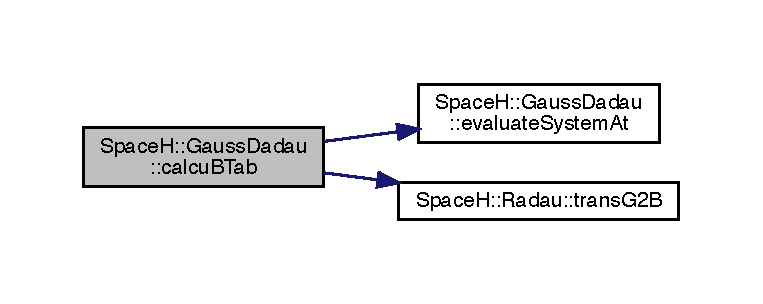
\includegraphics[width=350pt]{class_space_h_1_1_gauss_dadau_ac7089493b28c3c3ed67dc875e172b40c_cgraph}
\end{center}
\end{figure}
Here is the caller graph for this function\+:
\nopagebreak
\begin{figure}[H]
\begin{center}
\leavevmode
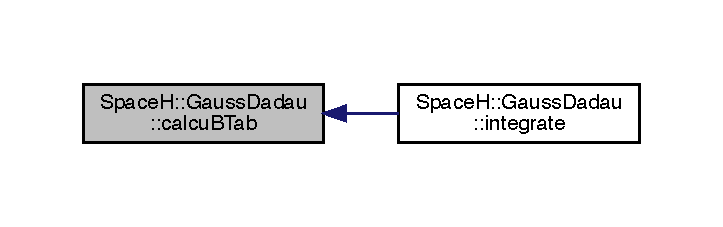
\includegraphics[width=347pt]{class_space_h_1_1_gauss_dadau_ac7089493b28c3c3ed67dc875e172b40c_icgraph}
\end{center}
\end{figure}
\mbox{\Hypertarget{class_space_h_1_1_gauss_dadau_a0e5f1df629baf9e5dfdfa052544c68ff}\label{class_space_h_1_1_gauss_dadau_a0e5f1df629baf9e5dfdfa052544c68ff}} 
\index{Space\+H\+::\+Gauss\+Dadau@{Space\+H\+::\+Gauss\+Dadau}!check\+Tab\+Volume@{check\+Tab\+Volume}}
\index{check\+Tab\+Volume@{check\+Tab\+Volume}!Space\+H\+::\+Gauss\+Dadau@{Space\+H\+::\+Gauss\+Dadau}}
\subsubsection{\texorpdfstring{check\+Tab\+Volume()}{checkTabVolume()}\hspace{0.1cm}{\footnotesize\ttfamily [1/2]}}
{\footnotesize\ttfamily template$<$typename Partic\+Sys $>$ \\
template$<$size\+\_\+t is\+D\+Y\+N\+A\+M\+I\+C\+AL$>$ \\
std\+::enable\+\_\+if$<$is\+D\+Y\+N\+A\+M\+I\+C\+AL != \mbox{\hyperlink{namespace_space_h_a3e55b9bc2a9e10c08ce8121bce11244a}{Space\+H\+::\+D\+Y\+N\+A\+M\+I\+C\+AL}}$>$\+::\mbox{\hyperlink{class_space_h_1_1_gauss_dadau_a780629d19a82feeab959cd68c8a5f8a3}{type}} \mbox{\hyperlink{class_space_h_1_1_gauss_dadau}{Space\+H\+::\+Gauss\+Dadau}}$<$ Partic\+Sys $>$\+::check\+Tab\+Volume (\begin{DoxyParamCaption}\item[{size\+\_\+t}]{particle\+Num }\end{DoxyParamCaption})\hspace{0.3cm}{\ttfamily [inline]}}

\mbox{\Hypertarget{class_space_h_1_1_gauss_dadau_acd04be9569a1426f923714b6086598a5}\label{class_space_h_1_1_gauss_dadau_acd04be9569a1426f923714b6086598a5}} 
\index{Space\+H\+::\+Gauss\+Dadau@{Space\+H\+::\+Gauss\+Dadau}!check\+Tab\+Volume@{check\+Tab\+Volume}}
\index{check\+Tab\+Volume@{check\+Tab\+Volume}!Space\+H\+::\+Gauss\+Dadau@{Space\+H\+::\+Gauss\+Dadau}}
\subsubsection{\texorpdfstring{check\+Tab\+Volume()}{checkTabVolume()}\hspace{0.1cm}{\footnotesize\ttfamily [2/2]}}
{\footnotesize\ttfamily template$<$typename Partic\+Sys $>$ \\
template$<$size\+\_\+t is\+D\+Y\+N\+A\+M\+I\+C\+AL$>$ \\
std\+::enable\+\_\+if$<$is\+D\+Y\+N\+A\+M\+I\+C\+AL == \mbox{\hyperlink{namespace_space_h_a3e55b9bc2a9e10c08ce8121bce11244a}{Space\+H\+::\+D\+Y\+N\+A\+M\+I\+C\+AL}}$>$\+::\mbox{\hyperlink{class_space_h_1_1_gauss_dadau_a780629d19a82feeab959cd68c8a5f8a3}{type}} \mbox{\hyperlink{class_space_h_1_1_gauss_dadau}{Space\+H\+::\+Gauss\+Dadau}}$<$ Partic\+Sys $>$\+::check\+Tab\+Volume (\begin{DoxyParamCaption}\item[{size\+\_\+t}]{particle\+Num }\end{DoxyParamCaption})\hspace{0.3cm}{\ttfamily [inline]}}

\mbox{\Hypertarget{class_space_h_1_1_gauss_dadau_a135095dd4f33570045a327dec46e6840}\label{class_space_h_1_1_gauss_dadau_a135095dd4f33570045a327dec46e6840}} 
\index{Space\+H\+::\+Gauss\+Dadau@{Space\+H\+::\+Gauss\+Dadau}!evaluate\+System\+At@{evaluate\+System\+At}}
\index{evaluate\+System\+At@{evaluate\+System\+At}!Space\+H\+::\+Gauss\+Dadau@{Space\+H\+::\+Gauss\+Dadau}}
\subsubsection{\texorpdfstring{evaluate\+System\+At()}{evaluateSystemAt()}}
{\footnotesize\ttfamily template$<$typename Partic\+Sys $>$ \\
void \mbox{\hyperlink{class_space_h_1_1_gauss_dadau}{Space\+H\+::\+Gauss\+Dadau}}$<$ Partic\+Sys $>$\+::evaluate\+System\+At (\begin{DoxyParamCaption}\item[{Partic\+Sys \&}]{particle\+Sys,  }\item[{\mbox{\hyperlink{class_space_h_1_1_gauss_dadau_ace42540e9fb47d7f1d1f00622bbd1ccb}{Scalar}}}]{step\+Length,  }\item[{size\+\_\+t}]{index }\end{DoxyParamCaption})\hspace{0.3cm}{\ttfamily [inline]}}

Here is the caller graph for this function\+:
\nopagebreak
\begin{figure}[H]
\begin{center}
\leavevmode
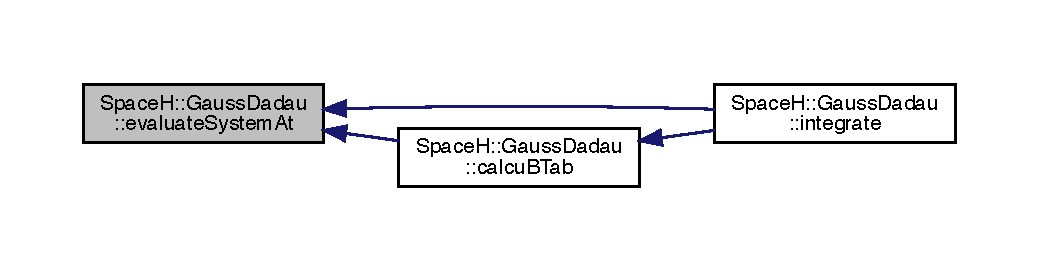
\includegraphics[width=350pt]{class_space_h_1_1_gauss_dadau_a135095dd4f33570045a327dec46e6840_icgraph}
\end{center}
\end{figure}
\mbox{\Hypertarget{class_space_h_1_1_gauss_dadau_acd80e3ae759660e91227ff4c83da01f1}\label{class_space_h_1_1_gauss_dadau_acd80e3ae759660e91227ff4c83da01f1}} 
\index{Space\+H\+::\+Gauss\+Dadau@{Space\+H\+::\+Gauss\+Dadau}!get\+B\+Tab@{get\+B\+Tab}}
\index{get\+B\+Tab@{get\+B\+Tab}!Space\+H\+::\+Gauss\+Dadau@{Space\+H\+::\+Gauss\+Dadau}}
\subsubsection{\texorpdfstring{get\+B\+Tab()}{getBTab()}}
{\footnotesize\ttfamily template$<$typename Partic\+Sys $>$ \\
const \mbox{\hyperlink{class_space_h_1_1_gauss_dadau_aa191c67a1447ce70b7ec2dae6b061176}{Radau\+Tab}}\& \mbox{\hyperlink{class_space_h_1_1_gauss_dadau}{Space\+H\+::\+Gauss\+Dadau}}$<$ Partic\+Sys $>$\+::get\+B\+Tab (\begin{DoxyParamCaption}{ }\end{DoxyParamCaption}) const\hspace{0.3cm}{\ttfamily [inline]}}

\mbox{\Hypertarget{class_space_h_1_1_gauss_dadau_a5ce29f965ea0376d9fb3fddf116926b1}\label{class_space_h_1_1_gauss_dadau_a5ce29f965ea0376d9fb3fddf116926b1}} 
\index{Space\+H\+::\+Gauss\+Dadau@{Space\+H\+::\+Gauss\+Dadau}!integrate@{integrate}}
\index{integrate@{integrate}!Space\+H\+::\+Gauss\+Dadau@{Space\+H\+::\+Gauss\+Dadau}}
\subsubsection{\texorpdfstring{integrate()}{integrate()}}
{\footnotesize\ttfamily template$<$typename Partic\+Sys $>$ \\
void \mbox{\hyperlink{class_space_h_1_1_gauss_dadau}{Space\+H\+::\+Gauss\+Dadau}}$<$ Partic\+Sys $>$\+::integrate (\begin{DoxyParamCaption}\item[{Partic\+Sys \&}]{particles,  }\item[{\mbox{\hyperlink{class_space_h_1_1_gauss_dadau_ace42540e9fb47d7f1d1f00622bbd1ccb}{Scalar}}}]{step\+Length }\end{DoxyParamCaption})\hspace{0.3cm}{\ttfamily [inline]}}



Interface to integrate particle system. 

This function integrate the particle system for one step with Gauss-\/\+Radau stepping. 
\begin{DoxyParams}{Parameters}
{\em particles} & \mbox{\hyperlink{struct_space_h_1_1_particle}{Particle}} system need to be integrated. \\
\hline
{\em step\+Length} & Step size for integration. \\
\hline
\end{DoxyParams}
Here is the call graph for this function\+:
\nopagebreak
\begin{figure}[H]
\begin{center}
\leavevmode
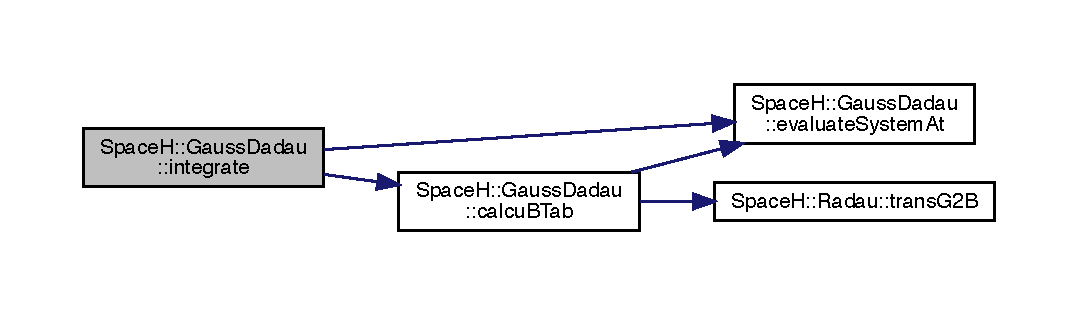
\includegraphics[width=350pt]{class_space_h_1_1_gauss_dadau_a5ce29f965ea0376d9fb3fddf116926b1_cgraph}
\end{center}
\end{figure}
\mbox{\Hypertarget{class_space_h_1_1_gauss_dadau_a9e89b65584577e684033159d85aa1a9f}\label{class_space_h_1_1_gauss_dadau_a9e89b65584577e684033159d85aa1a9f}} 
\index{Space\+H\+::\+Gauss\+Dadau@{Space\+H\+::\+Gauss\+Dadau}!local\+Acc@{local\+Acc}}
\index{local\+Acc@{local\+Acc}!Space\+H\+::\+Gauss\+Dadau@{Space\+H\+::\+Gauss\+Dadau}}
\subsubsection{\texorpdfstring{local\+Acc()}{localAcc()}}
{\footnotesize\ttfamily template$<$typename Partic\+Sys $>$ \\
const \mbox{\hyperlink{class_space_h_1_1_gauss_dadau_a69e00c49f96f4ffeeb767bb7222834da}{Vector\+Array}}\& \mbox{\hyperlink{class_space_h_1_1_gauss_dadau}{Space\+H\+::\+Gauss\+Dadau}}$<$ Partic\+Sys $>$\+::local\+Acc (\begin{DoxyParamCaption}{ }\end{DoxyParamCaption}) const\hspace{0.3cm}{\ttfamily [inline]}}

\mbox{\Hypertarget{class_space_h_1_1_gauss_dadau_a7669fef19d9982793fc4f4bbd49ad650}\label{class_space_h_1_1_gauss_dadau_a7669fef19d9982793fc4f4bbd49ad650}} 
\index{Space\+H\+::\+Gauss\+Dadau@{Space\+H\+::\+Gauss\+Dadau}!predict\+NewB@{predict\+NewB}}
\index{predict\+NewB@{predict\+NewB}!Space\+H\+::\+Gauss\+Dadau@{Space\+H\+::\+Gauss\+Dadau}}
\subsubsection{\texorpdfstring{predict\+New\+B()}{predictNewB()}}
{\footnotesize\ttfamily template$<$typename Partic\+Sys $>$ \\
void \mbox{\hyperlink{class_space_h_1_1_gauss_dadau}{Space\+H\+::\+Gauss\+Dadau}}$<$ Partic\+Sys $>$\+::predict\+NewB (\begin{DoxyParamCaption}\item[{\mbox{\hyperlink{class_space_h_1_1_gauss_dadau_ace42540e9fb47d7f1d1f00622bbd1ccb}{Scalar}}}]{Q1 }\end{DoxyParamCaption})\hspace{0.3cm}{\ttfamily [inline]}}



\subsection{Member Data Documentation}
\mbox{\Hypertarget{class_space_h_1_1_gauss_dadau_ac671afa9ebffbf85891ba283076d04f1}\label{class_space_h_1_1_gauss_dadau_ac671afa9ebffbf85891ba283076d04f1}} 
\index{Space\+H\+::\+Gauss\+Dadau@{Space\+H\+::\+Gauss\+Dadau}!final\+Point@{final\+Point}}
\index{final\+Point@{final\+Point}!Space\+H\+::\+Gauss\+Dadau@{Space\+H\+::\+Gauss\+Dadau}}
\subsubsection{\texorpdfstring{final\+Point}{finalPoint}}
{\footnotesize\ttfamily template$<$typename Partic\+Sys $>$ \\
const size\+\_\+t \mbox{\hyperlink{class_space_h_1_1_gauss_dadau}{Space\+H\+::\+Gauss\+Dadau}}$<$ Partic\+Sys $>$\+::final\+Point \{7\}\hspace{0.3cm}{\ttfamily [static]}}

\mbox{\Hypertarget{class_space_h_1_1_gauss_dadau_aa306d2c64787f9a38901bdddc791c938}\label{class_space_h_1_1_gauss_dadau_aa306d2c64787f9a38901bdddc791c938}} 
\index{Space\+H\+::\+Gauss\+Dadau@{Space\+H\+::\+Gauss\+Dadau}!order@{order}}
\index{order@{order}!Space\+H\+::\+Gauss\+Dadau@{Space\+H\+::\+Gauss\+Dadau}}
\subsubsection{\texorpdfstring{order}{order}}
{\footnotesize\ttfamily template$<$typename Partic\+Sys $>$ \\
const int \mbox{\hyperlink{class_space_h_1_1_gauss_dadau}{Space\+H\+::\+Gauss\+Dadau}}$<$ Partic\+Sys $>$\+::order \{15\}\hspace{0.3cm}{\ttfamily [static]}}



Order of the integrator. 



The documentation for this class was generated from the following file\+:\begin{DoxyCompactItemize}
\item 
integrator/\mbox{\hyperlink{_gauss-_dadau_8h}{Gauss-\/\+Dadau.\+h}}\end{DoxyCompactItemize}

\hypertarget{struct_space_h_1_1get__value__type}{}\section{SpaceH\+:\+:get\+\_\+value\+\_\+type$<$ T $>$ Struct Template Reference}
\label{struct_space_h_1_1get__value__type}\index{Space\+H\+::get\+\_\+value\+\_\+type$<$ T $>$@{Space\+H\+::get\+\_\+value\+\_\+type$<$ T $>$}}


{\ttfamily \#include $<$dev\+Tools.\+h$>$}

\subsection*{Public Types}
\begin{DoxyCompactItemize}
\item 
using \mbox{\hyperlink{struct_space_h_1_1get__value__type_a22e0b1ebb5f91bb129a9487208ebd7c7}{type}} = decltype(check$<$ T $>$(0))
\end{DoxyCompactItemize}


\subsection{Member Typedef Documentation}
\mbox{\Hypertarget{struct_space_h_1_1get__value__type_a22e0b1ebb5f91bb129a9487208ebd7c7}\label{struct_space_h_1_1get__value__type_a22e0b1ebb5f91bb129a9487208ebd7c7}} 
\index{Space\+H\+::get\+\_\+value\+\_\+type@{Space\+H\+::get\+\_\+value\+\_\+type}!type@{type}}
\index{type@{type}!Space\+H\+::get\+\_\+value\+\_\+type@{Space\+H\+::get\+\_\+value\+\_\+type}}
\subsubsection{\texorpdfstring{type}{type}}
{\footnotesize\ttfamily template$<$typename T$>$ \\
using \mbox{\hyperlink{struct_space_h_1_1get__value__type}{Space\+H\+::get\+\_\+value\+\_\+type}}$<$ T $>$\+::\mbox{\hyperlink{struct_space_h_1_1get__value__type_a22e0b1ebb5f91bb129a9487208ebd7c7}{type}} =  decltype(check$<$T$>$(0))}



The documentation for this struct was generated from the following file\+:\begin{DoxyCompactItemize}
\item 
\mbox{\hyperlink{dev_tools_8h}{dev\+Tools.\+h}}\end{DoxyCompactItemize}

\hypertarget{class_space_h_1_1_i_a_s15}{}\section{SpaceH\+:\+:I\+A\+S15$<$ Partic\+Sys, Integrator $>$ Class Template Reference}
\label{class_space_h_1_1_i_a_s15}\index{Space\+H\+::\+I\+A\+S15$<$ Partic\+Sys, Integrator $>$@{Space\+H\+::\+I\+A\+S15$<$ Partic\+Sys, Integrator $>$}}


\mbox{\hyperlink{class_space_h_1_1_i_a_s15}{I\+A\+S15}} iterator see details in \href{https://arxiv.org/abs/1409.4779}{\tt https\+://arxiv.\+org/abs/1409.\+4779} .  




{\ttfamily \#include $<$I\+A\+S15.\+h$>$}

\subsection*{Public Types}
\begin{DoxyCompactItemize}
\item 
using \mbox{\hyperlink{class_space_h_1_1_i_a_s15_aaa8ebb8060b4421b9bb799dfb0a0d21a}{type}} = typename Partic\+Sys\+::type
\item 
using \mbox{\hyperlink{class_space_h_1_1_i_a_s15_ac4ee5f40852d7b500ca50084eb35b012}{Scalar}} = typename type\+::\+Scalar
\item 
using \mbox{\hyperlink{class_space_h_1_1_i_a_s15_ae34d12477ecdc0742911fc95748e5fd8}{Vector}} = typename type\+::\+Vector
\item 
using \mbox{\hyperlink{class_space_h_1_1_i_a_s15_a70aa5a3879ee4da4472dbeca219f9b3f}{Vector\+Array}} = typename type\+::\+Vector\+Array
\item 
using \mbox{\hyperlink{class_space_h_1_1_i_a_s15_a17ef1472c0db7e9fdafffed41e5b9a3b}{Scalar\+Buffer}} = typename type\+::\+Scalar\+Buffer
\item 
using \mbox{\hyperlink{class_space_h_1_1_i_a_s15_a1eda622ee773ed5b2dff783600e1f7f7}{Radau\+Array}} = typename Integrator\+::\+Radau\+Array
\item 
using \mbox{\hyperlink{class_space_h_1_1_i_a_s15_a4023c69d2644098aa8d75181f6a82fc7}{Radau\+Tab}} = typename Integrator\+::\+Radau\+Tab
\end{DoxyCompactItemize}
\subsection*{Public Member Functions}
\begin{DoxyCompactItemize}
\item 
\mbox{\hyperlink{class_space_h_1_1_i_a_s15_ac4ee5f40852d7b500ca50084eb35b012}{Scalar}} \mbox{\hyperlink{class_space_h_1_1_i_a_s15_a60d1a4d8ab5124bf3adc12624f1d7954}{iterate}} (Partic\+Sys \&particles, \mbox{\hyperlink{class_space_h_1_1_i_a_s15_ac4ee5f40852d7b500ca50084eb35b012}{Scalar}} step\+Length)
\begin{DoxyCompactList}\small\item\em interface to iterate particle system for one step \end{DoxyCompactList}\item 
void \mbox{\hyperlink{class_space_h_1_1_i_a_s15_a05a4ea53a8d39fc77fc761f7a8a9864d}{set\+Relative\+Error}} (\mbox{\hyperlink{class_space_h_1_1_i_a_s15_ac4ee5f40852d7b500ca50084eb35b012}{Scalar}} rel\+\_\+tol)
\item 
void \mbox{\hyperlink{class_space_h_1_1_i_a_s15_a7897b1d71c67cd47c5559f6997a9d487}{Set\+Convergent\+Limit}} (\mbox{\hyperlink{class_space_h_1_1_i_a_s15_ac4ee5f40852d7b500ca50084eb35b012}{Scalar}} limit)
\end{DoxyCompactItemize}


\subsection{Detailed Description}
\subsubsection*{template$<$typename Partic\+Sys, typename Integrator$>$\newline
class Space\+H\+::\+I\+A\+S15$<$ Partic\+Sys, Integrator $>$}

\mbox{\hyperlink{class_space_h_1_1_i_a_s15}{I\+A\+S15}} iterator see details in \href{https://arxiv.org/abs/1409.4779}{\tt https\+://arxiv.\+org/abs/1409.\+4779} . 



\subsection{Member Typedef Documentation}
\mbox{\Hypertarget{class_space_h_1_1_i_a_s15_a1eda622ee773ed5b2dff783600e1f7f7}\label{class_space_h_1_1_i_a_s15_a1eda622ee773ed5b2dff783600e1f7f7}} 
\index{Space\+H\+::\+I\+A\+S15@{Space\+H\+::\+I\+A\+S15}!Radau\+Array@{Radau\+Array}}
\index{Radau\+Array@{Radau\+Array}!Space\+H\+::\+I\+A\+S15@{Space\+H\+::\+I\+A\+S15}}
\subsubsection{\texorpdfstring{Radau\+Array}{RadauArray}}
{\footnotesize\ttfamily template$<$typename Partic\+Sys , typename Integrator $>$ \\
using \mbox{\hyperlink{class_space_h_1_1_i_a_s15}{Space\+H\+::\+I\+A\+S15}}$<$ Partic\+Sys, Integrator $>$\+::\mbox{\hyperlink{class_space_h_1_1_i_a_s15_a1eda622ee773ed5b2dff783600e1f7f7}{Radau\+Array}} =  typename Integrator\+::\+Radau\+Array}

\mbox{\Hypertarget{class_space_h_1_1_i_a_s15_a4023c69d2644098aa8d75181f6a82fc7}\label{class_space_h_1_1_i_a_s15_a4023c69d2644098aa8d75181f6a82fc7}} 
\index{Space\+H\+::\+I\+A\+S15@{Space\+H\+::\+I\+A\+S15}!Radau\+Tab@{Radau\+Tab}}
\index{Radau\+Tab@{Radau\+Tab}!Space\+H\+::\+I\+A\+S15@{Space\+H\+::\+I\+A\+S15}}
\subsubsection{\texorpdfstring{Radau\+Tab}{RadauTab}}
{\footnotesize\ttfamily template$<$typename Partic\+Sys , typename Integrator $>$ \\
using \mbox{\hyperlink{class_space_h_1_1_i_a_s15}{Space\+H\+::\+I\+A\+S15}}$<$ Partic\+Sys, Integrator $>$\+::\mbox{\hyperlink{class_space_h_1_1_i_a_s15_a4023c69d2644098aa8d75181f6a82fc7}{Radau\+Tab}} =  typename Integrator\+::\+Radau\+Tab}

\mbox{\Hypertarget{class_space_h_1_1_i_a_s15_ac4ee5f40852d7b500ca50084eb35b012}\label{class_space_h_1_1_i_a_s15_ac4ee5f40852d7b500ca50084eb35b012}} 
\index{Space\+H\+::\+I\+A\+S15@{Space\+H\+::\+I\+A\+S15}!Scalar@{Scalar}}
\index{Scalar@{Scalar}!Space\+H\+::\+I\+A\+S15@{Space\+H\+::\+I\+A\+S15}}
\subsubsection{\texorpdfstring{Scalar}{Scalar}}
{\footnotesize\ttfamily template$<$typename Partic\+Sys , typename Integrator $>$ \\
using \mbox{\hyperlink{class_space_h_1_1_i_a_s15}{Space\+H\+::\+I\+A\+S15}}$<$ Partic\+Sys, Integrator $>$\+::\mbox{\hyperlink{class_space_h_1_1_i_a_s15_ac4ee5f40852d7b500ca50084eb35b012}{Scalar}} =  typename type\+::\+Scalar}

\mbox{\Hypertarget{class_space_h_1_1_i_a_s15_a17ef1472c0db7e9fdafffed41e5b9a3b}\label{class_space_h_1_1_i_a_s15_a17ef1472c0db7e9fdafffed41e5b9a3b}} 
\index{Space\+H\+::\+I\+A\+S15@{Space\+H\+::\+I\+A\+S15}!Scalar\+Buffer@{Scalar\+Buffer}}
\index{Scalar\+Buffer@{Scalar\+Buffer}!Space\+H\+::\+I\+A\+S15@{Space\+H\+::\+I\+A\+S15}}
\subsubsection{\texorpdfstring{Scalar\+Buffer}{ScalarBuffer}}
{\footnotesize\ttfamily template$<$typename Partic\+Sys , typename Integrator $>$ \\
using \mbox{\hyperlink{class_space_h_1_1_i_a_s15}{Space\+H\+::\+I\+A\+S15}}$<$ Partic\+Sys, Integrator $>$\+::\mbox{\hyperlink{class_space_h_1_1_i_a_s15_a17ef1472c0db7e9fdafffed41e5b9a3b}{Scalar\+Buffer}} =  typename type\+::\+Scalar\+Buffer}

\mbox{\Hypertarget{class_space_h_1_1_i_a_s15_aaa8ebb8060b4421b9bb799dfb0a0d21a}\label{class_space_h_1_1_i_a_s15_aaa8ebb8060b4421b9bb799dfb0a0d21a}} 
\index{Space\+H\+::\+I\+A\+S15@{Space\+H\+::\+I\+A\+S15}!type@{type}}
\index{type@{type}!Space\+H\+::\+I\+A\+S15@{Space\+H\+::\+I\+A\+S15}}
\subsubsection{\texorpdfstring{type}{type}}
{\footnotesize\ttfamily template$<$typename Partic\+Sys , typename Integrator $>$ \\
using \mbox{\hyperlink{class_space_h_1_1_i_a_s15}{Space\+H\+::\+I\+A\+S15}}$<$ Partic\+Sys, Integrator $>$\+::\mbox{\hyperlink{class_space_h_1_1_i_a_s15_aaa8ebb8060b4421b9bb799dfb0a0d21a}{type}} =  typename Partic\+Sys\+::type}

\mbox{\Hypertarget{class_space_h_1_1_i_a_s15_ae34d12477ecdc0742911fc95748e5fd8}\label{class_space_h_1_1_i_a_s15_ae34d12477ecdc0742911fc95748e5fd8}} 
\index{Space\+H\+::\+I\+A\+S15@{Space\+H\+::\+I\+A\+S15}!Vector@{Vector}}
\index{Vector@{Vector}!Space\+H\+::\+I\+A\+S15@{Space\+H\+::\+I\+A\+S15}}
\subsubsection{\texorpdfstring{Vector}{Vector}}
{\footnotesize\ttfamily template$<$typename Partic\+Sys , typename Integrator $>$ \\
using \mbox{\hyperlink{class_space_h_1_1_i_a_s15}{Space\+H\+::\+I\+A\+S15}}$<$ Partic\+Sys, Integrator $>$\+::\mbox{\hyperlink{class_space_h_1_1_i_a_s15_ae34d12477ecdc0742911fc95748e5fd8}{Vector}} =  typename type\+::\+Vector}

\mbox{\Hypertarget{class_space_h_1_1_i_a_s15_a70aa5a3879ee4da4472dbeca219f9b3f}\label{class_space_h_1_1_i_a_s15_a70aa5a3879ee4da4472dbeca219f9b3f}} 
\index{Space\+H\+::\+I\+A\+S15@{Space\+H\+::\+I\+A\+S15}!Vector\+Array@{Vector\+Array}}
\index{Vector\+Array@{Vector\+Array}!Space\+H\+::\+I\+A\+S15@{Space\+H\+::\+I\+A\+S15}}
\subsubsection{\texorpdfstring{Vector\+Array}{VectorArray}}
{\footnotesize\ttfamily template$<$typename Partic\+Sys , typename Integrator $>$ \\
using \mbox{\hyperlink{class_space_h_1_1_i_a_s15}{Space\+H\+::\+I\+A\+S15}}$<$ Partic\+Sys, Integrator $>$\+::\mbox{\hyperlink{class_space_h_1_1_i_a_s15_a70aa5a3879ee4da4472dbeca219f9b3f}{Vector\+Array}} =  typename type\+::\+Vector\+Array}



\subsection{Member Function Documentation}
\mbox{\Hypertarget{class_space_h_1_1_i_a_s15_a60d1a4d8ab5124bf3adc12624f1d7954}\label{class_space_h_1_1_i_a_s15_a60d1a4d8ab5124bf3adc12624f1d7954}} 
\index{Space\+H\+::\+I\+A\+S15@{Space\+H\+::\+I\+A\+S15}!iterate@{iterate}}
\index{iterate@{iterate}!Space\+H\+::\+I\+A\+S15@{Space\+H\+::\+I\+A\+S15}}
\subsubsection{\texorpdfstring{iterate()}{iterate()}}
{\footnotesize\ttfamily template$<$typename Partic\+Sys , typename Integrator $>$ \\
\mbox{\hyperlink{class_space_h_1_1_i_a_s15_ac4ee5f40852d7b500ca50084eb35b012}{Scalar}} \mbox{\hyperlink{class_space_h_1_1_i_a_s15}{Space\+H\+::\+I\+A\+S15}}$<$ Partic\+Sys, Integrator $>$\+::iterate (\begin{DoxyParamCaption}\item[{Partic\+Sys \&}]{particles,  }\item[{\mbox{\hyperlink{class_space_h_1_1_i_a_s15_ac4ee5f40852d7b500ca50084eb35b012}{Scalar}}}]{step\+Length }\end{DoxyParamCaption})\hspace{0.3cm}{\ttfamily [inline]}}



interface to iterate particle system for one step 


\begin{DoxyParams}{Parameters}
{\em particles} & \mbox{\hyperlink{struct_space_h_1_1_particle}{Particle}} system needs evolution. \\
\hline
{\em integrator} & Integrator to integrate the particle system. \\
\hline
{\em step\+Length} & Macro step length for iteration(\+Here, the step length of the integrator). \\
\hline
\end{DoxyParams}
\begin{DoxyReturn}{Returns}
step length for next iteration. 
\end{DoxyReturn}
Here is the call graph for this function\+:
\nopagebreak
\begin{figure}[H]
\begin{center}
\leavevmode
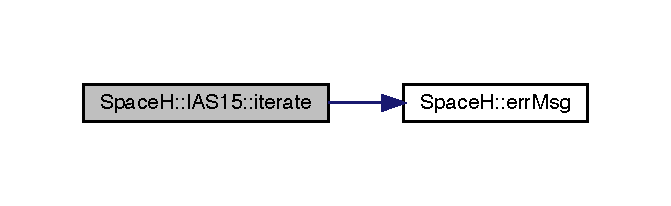
\includegraphics[width=322pt]{class_space_h_1_1_i_a_s15_a60d1a4d8ab5124bf3adc12624f1d7954_cgraph}
\end{center}
\end{figure}
\mbox{\Hypertarget{class_space_h_1_1_i_a_s15_a7897b1d71c67cd47c5559f6997a9d487}\label{class_space_h_1_1_i_a_s15_a7897b1d71c67cd47c5559f6997a9d487}} 
\index{Space\+H\+::\+I\+A\+S15@{Space\+H\+::\+I\+A\+S15}!Set\+Convergent\+Limit@{Set\+Convergent\+Limit}}
\index{Set\+Convergent\+Limit@{Set\+Convergent\+Limit}!Space\+H\+::\+I\+A\+S15@{Space\+H\+::\+I\+A\+S15}}
\subsubsection{\texorpdfstring{Set\+Convergent\+Limit()}{SetConvergentLimit()}}
{\footnotesize\ttfamily template$<$typename Partic\+Sys , typename Integrator $>$ \\
void \mbox{\hyperlink{class_space_h_1_1_i_a_s15}{Space\+H\+::\+I\+A\+S15}}$<$ Partic\+Sys, Integrator $>$\+::Set\+Convergent\+Limit (\begin{DoxyParamCaption}\item[{\mbox{\hyperlink{class_space_h_1_1_i_a_s15_ac4ee5f40852d7b500ca50084eb35b012}{Scalar}}}]{limit }\end{DoxyParamCaption})\hspace{0.3cm}{\ttfamily [inline]}}

\mbox{\Hypertarget{class_space_h_1_1_i_a_s15_a05a4ea53a8d39fc77fc761f7a8a9864d}\label{class_space_h_1_1_i_a_s15_a05a4ea53a8d39fc77fc761f7a8a9864d}} 
\index{Space\+H\+::\+I\+A\+S15@{Space\+H\+::\+I\+A\+S15}!set\+Relative\+Error@{set\+Relative\+Error}}
\index{set\+Relative\+Error@{set\+Relative\+Error}!Space\+H\+::\+I\+A\+S15@{Space\+H\+::\+I\+A\+S15}}
\subsubsection{\texorpdfstring{set\+Relative\+Error()}{setRelativeError()}}
{\footnotesize\ttfamily template$<$typename Partic\+Sys , typename Integrator $>$ \\
void \mbox{\hyperlink{class_space_h_1_1_i_a_s15}{Space\+H\+::\+I\+A\+S15}}$<$ Partic\+Sys, Integrator $>$\+::set\+Relative\+Error (\begin{DoxyParamCaption}\item[{\mbox{\hyperlink{class_space_h_1_1_i_a_s15_ac4ee5f40852d7b500ca50084eb35b012}{Scalar}}}]{rel\+\_\+tol }\end{DoxyParamCaption})\hspace{0.3cm}{\ttfamily [inline]}}



The documentation for this class was generated from the following file\+:\begin{DoxyCompactItemize}
\item 
O\+D\+Eiterator/\mbox{\hyperlink{_i_a_s15_8h}{I\+A\+S15.\+h}}\end{DoxyCompactItemize}

\hypertarget{class_space_h_1_1_init_creator}{}\section{SpaceH\+:\+:Init\+Creator$<$ Particle $>$ Class Template Reference}
\label{class_space_h_1_1_init_creator}\index{Space\+H\+::\+Init\+Creator$<$ Particle $>$@{Space\+H\+::\+Init\+Creator$<$ Particle $>$}}


{\ttfamily \#include $<$Init\+File\+Creator.\+h$>$}

\subsection*{Public Types}
\begin{DoxyCompactItemize}
\item 
using \mbox{\hyperlink{class_space_h_1_1_init_creator_abe67b1be453e00e5ce5d84fe0755cf24}{type}} = typename \mbox{\hyperlink{struct_space_h_1_1_particle_a4da7db09bcfc01d24c63468e6e08fa24}{Particle\+::type}}
\item 
using \mbox{\hyperlink{class_space_h_1_1_init_creator_ac049ccad04f7cd33cc95b17ad763a988}{Scalar}} = typename type\+::\+Scalar
\item 
using \mbox{\hyperlink{class_space_h_1_1_init_creator_ad355713fe020ed2c9fb0007cb4340340}{Vector}} = typename type\+::\+Vector
\item 
{\footnotesize template$<$typename T , size\+\_\+t S$>$ }\\using \mbox{\hyperlink{class_space_h_1_1_init_creator_a6e484fb8b2f46a2b1c4a54b782dec9d8}{Container}} = typename type\+::template \mbox{\hyperlink{class_space_h_1_1_init_creator_a6e484fb8b2f46a2b1c4a54b782dec9d8}{Container}}$<$ T, S $>$
\end{DoxyCompactItemize}
\subsection*{Public Member Functions}
\begin{DoxyCompactItemize}
\item 
void \mbox{\hyperlink{class_space_h_1_1_init_creator_a6cf46010b11b3b7ad19f1d37e2cb1cb4}{write\+To\+File}} (const char $\ast$file\+Path, \mbox{\hyperlink{class_space_h_1_1_init_creator_ac049ccad04f7cd33cc95b17ad763a988}{Scalar}} time=0)
\item 
void \mbox{\hyperlink{class_space_h_1_1_init_creator_a3d0b62c72c0bd432ca93ec3ec60f6153}{add\+Particle}} (const \mbox{\hyperlink{struct_space_h_1_1_particle}{Particle}} \&new\+Particle)
\item 
size\+\_\+t \mbox{\hyperlink{class_space_h_1_1_init_creator_ad6dde97c265c5336f5d9e16b36dfad5c}{particle\+Number}} ()
\item 
const \mbox{\hyperlink{struct_space_h_1_1_particle}{Particle}} \& \mbox{\hyperlink{class_space_h_1_1_init_creator_a3de1c9fb8bfd533fe69aa782d8d1bcb8}{operator\mbox{[}$\,$\mbox{]}}} (size\+\_\+t i) const
\item 
void \mbox{\hyperlink{class_space_h_1_1_init_creator_aa54d6696d3cd8cab4db3a284aaeb54ca}{clear}} ()
\end{DoxyCompactItemize}


\subsection{Member Typedef Documentation}
\mbox{\Hypertarget{class_space_h_1_1_init_creator_a6e484fb8b2f46a2b1c4a54b782dec9d8}\label{class_space_h_1_1_init_creator_a6e484fb8b2f46a2b1c4a54b782dec9d8}} 
\index{Space\+H\+::\+Init\+Creator@{Space\+H\+::\+Init\+Creator}!Container@{Container}}
\index{Container@{Container}!Space\+H\+::\+Init\+Creator@{Space\+H\+::\+Init\+Creator}}
\subsubsection{\texorpdfstring{Container}{Container}}
{\footnotesize\ttfamily template$<$typename Particle $>$ \\
template$<$typename T , size\+\_\+t S$>$ \\
using \mbox{\hyperlink{class_space_h_1_1_init_creator}{Space\+H\+::\+Init\+Creator}}$<$ \mbox{\hyperlink{struct_space_h_1_1_particle}{Particle}} $>$\+::\mbox{\hyperlink{class_space_h_1_1_init_creator_a6e484fb8b2f46a2b1c4a54b782dec9d8}{Container}} =  typename type\+::template \mbox{\hyperlink{class_space_h_1_1_init_creator_a6e484fb8b2f46a2b1c4a54b782dec9d8}{Container}}$<$T, S$>$}

\mbox{\Hypertarget{class_space_h_1_1_init_creator_ac049ccad04f7cd33cc95b17ad763a988}\label{class_space_h_1_1_init_creator_ac049ccad04f7cd33cc95b17ad763a988}} 
\index{Space\+H\+::\+Init\+Creator@{Space\+H\+::\+Init\+Creator}!Scalar@{Scalar}}
\index{Scalar@{Scalar}!Space\+H\+::\+Init\+Creator@{Space\+H\+::\+Init\+Creator}}
\subsubsection{\texorpdfstring{Scalar}{Scalar}}
{\footnotesize\ttfamily template$<$typename Particle $>$ \\
using \mbox{\hyperlink{class_space_h_1_1_init_creator}{Space\+H\+::\+Init\+Creator}}$<$ \mbox{\hyperlink{struct_space_h_1_1_particle}{Particle}} $>$\+::\mbox{\hyperlink{class_space_h_1_1_init_creator_ac049ccad04f7cd33cc95b17ad763a988}{Scalar}} =  typename type\+::\+Scalar}

\mbox{\Hypertarget{class_space_h_1_1_init_creator_abe67b1be453e00e5ce5d84fe0755cf24}\label{class_space_h_1_1_init_creator_abe67b1be453e00e5ce5d84fe0755cf24}} 
\index{Space\+H\+::\+Init\+Creator@{Space\+H\+::\+Init\+Creator}!type@{type}}
\index{type@{type}!Space\+H\+::\+Init\+Creator@{Space\+H\+::\+Init\+Creator}}
\subsubsection{\texorpdfstring{type}{type}}
{\footnotesize\ttfamily template$<$typename Particle $>$ \\
using \mbox{\hyperlink{class_space_h_1_1_init_creator}{Space\+H\+::\+Init\+Creator}}$<$ \mbox{\hyperlink{struct_space_h_1_1_particle}{Particle}} $>$\+::\mbox{\hyperlink{class_space_h_1_1_init_creator_abe67b1be453e00e5ce5d84fe0755cf24}{type}} =  typename \mbox{\hyperlink{struct_space_h_1_1_particle_a4da7db09bcfc01d24c63468e6e08fa24}{Particle\+::type}}}

\mbox{\Hypertarget{class_space_h_1_1_init_creator_ad355713fe020ed2c9fb0007cb4340340}\label{class_space_h_1_1_init_creator_ad355713fe020ed2c9fb0007cb4340340}} 
\index{Space\+H\+::\+Init\+Creator@{Space\+H\+::\+Init\+Creator}!Vector@{Vector}}
\index{Vector@{Vector}!Space\+H\+::\+Init\+Creator@{Space\+H\+::\+Init\+Creator}}
\subsubsection{\texorpdfstring{Vector}{Vector}}
{\footnotesize\ttfamily template$<$typename Particle $>$ \\
using \mbox{\hyperlink{class_space_h_1_1_init_creator}{Space\+H\+::\+Init\+Creator}}$<$ \mbox{\hyperlink{struct_space_h_1_1_particle}{Particle}} $>$\+::\mbox{\hyperlink{class_space_h_1_1_init_creator_ad355713fe020ed2c9fb0007cb4340340}{Vector}} =  typename type\+::\+Vector}



\subsection{Member Function Documentation}
\mbox{\Hypertarget{class_space_h_1_1_init_creator_a3d0b62c72c0bd432ca93ec3ec60f6153}\label{class_space_h_1_1_init_creator_a3d0b62c72c0bd432ca93ec3ec60f6153}} 
\index{Space\+H\+::\+Init\+Creator@{Space\+H\+::\+Init\+Creator}!add\+Particle@{add\+Particle}}
\index{add\+Particle@{add\+Particle}!Space\+H\+::\+Init\+Creator@{Space\+H\+::\+Init\+Creator}}
\subsubsection{\texorpdfstring{add\+Particle()}{addParticle()}}
{\footnotesize\ttfamily template$<$typename Particle $>$ \\
void \mbox{\hyperlink{class_space_h_1_1_init_creator}{Space\+H\+::\+Init\+Creator}}$<$ \mbox{\hyperlink{struct_space_h_1_1_particle}{Particle}} $>$\+::add\+Particle (\begin{DoxyParamCaption}\item[{const \mbox{\hyperlink{struct_space_h_1_1_particle}{Particle}} \&}]{new\+Particle }\end{DoxyParamCaption})\hspace{0.3cm}{\ttfamily [inline]}}

Here is the caller graph for this function\+:
\nopagebreak
\begin{figure}[H]
\begin{center}
\leavevmode
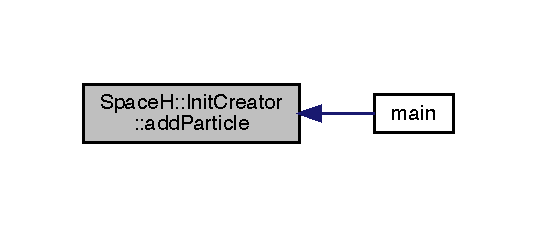
\includegraphics[width=257pt]{class_space_h_1_1_init_creator_a3d0b62c72c0bd432ca93ec3ec60f6153_icgraph}
\end{center}
\end{figure}
\mbox{\Hypertarget{class_space_h_1_1_init_creator_aa54d6696d3cd8cab4db3a284aaeb54ca}\label{class_space_h_1_1_init_creator_aa54d6696d3cd8cab4db3a284aaeb54ca}} 
\index{Space\+H\+::\+Init\+Creator@{Space\+H\+::\+Init\+Creator}!clear@{clear}}
\index{clear@{clear}!Space\+H\+::\+Init\+Creator@{Space\+H\+::\+Init\+Creator}}
\subsubsection{\texorpdfstring{clear()}{clear()}}
{\footnotesize\ttfamily template$<$typename Particle $>$ \\
void \mbox{\hyperlink{class_space_h_1_1_init_creator}{Space\+H\+::\+Init\+Creator}}$<$ \mbox{\hyperlink{struct_space_h_1_1_particle}{Particle}} $>$\+::clear (\begin{DoxyParamCaption}{ }\end{DoxyParamCaption})\hspace{0.3cm}{\ttfamily [inline]}}

\mbox{\Hypertarget{class_space_h_1_1_init_creator_a3de1c9fb8bfd533fe69aa782d8d1bcb8}\label{class_space_h_1_1_init_creator_a3de1c9fb8bfd533fe69aa782d8d1bcb8}} 
\index{Space\+H\+::\+Init\+Creator@{Space\+H\+::\+Init\+Creator}!operator\mbox{[}\mbox{]}@{operator[]}}
\index{operator\mbox{[}\mbox{]}@{operator[]}!Space\+H\+::\+Init\+Creator@{Space\+H\+::\+Init\+Creator}}
\subsubsection{\texorpdfstring{operator[]()}{operator[]()}}
{\footnotesize\ttfamily template$<$typename Particle $>$ \\
const \mbox{\hyperlink{struct_space_h_1_1_particle}{Particle}}\& \mbox{\hyperlink{class_space_h_1_1_init_creator}{Space\+H\+::\+Init\+Creator}}$<$ \mbox{\hyperlink{struct_space_h_1_1_particle}{Particle}} $>$\+::operator\mbox{[}$\,$\mbox{]} (\begin{DoxyParamCaption}\item[{size\+\_\+t}]{i }\end{DoxyParamCaption}) const\hspace{0.3cm}{\ttfamily [inline]}}

\mbox{\Hypertarget{class_space_h_1_1_init_creator_ad6dde97c265c5336f5d9e16b36dfad5c}\label{class_space_h_1_1_init_creator_ad6dde97c265c5336f5d9e16b36dfad5c}} 
\index{Space\+H\+::\+Init\+Creator@{Space\+H\+::\+Init\+Creator}!particle\+Number@{particle\+Number}}
\index{particle\+Number@{particle\+Number}!Space\+H\+::\+Init\+Creator@{Space\+H\+::\+Init\+Creator}}
\subsubsection{\texorpdfstring{particle\+Number()}{particleNumber()}}
{\footnotesize\ttfamily template$<$typename Particle $>$ \\
size\+\_\+t \mbox{\hyperlink{class_space_h_1_1_init_creator}{Space\+H\+::\+Init\+Creator}}$<$ \mbox{\hyperlink{struct_space_h_1_1_particle}{Particle}} $>$\+::particle\+Number (\begin{DoxyParamCaption}{ }\end{DoxyParamCaption})\hspace{0.3cm}{\ttfamily [inline]}}

Here is the caller graph for this function\+:
\nopagebreak
\begin{figure}[H]
\begin{center}
\leavevmode
\includegraphics[width=350pt]{class_space_h_1_1_init_creator_ad6dde97c265c5336f5d9e16b36dfad5c_icgraph}
\end{center}
\end{figure}
\mbox{\Hypertarget{class_space_h_1_1_init_creator_a6cf46010b11b3b7ad19f1d37e2cb1cb4}\label{class_space_h_1_1_init_creator_a6cf46010b11b3b7ad19f1d37e2cb1cb4}} 
\index{Space\+H\+::\+Init\+Creator@{Space\+H\+::\+Init\+Creator}!write\+To\+File@{write\+To\+File}}
\index{write\+To\+File@{write\+To\+File}!Space\+H\+::\+Init\+Creator@{Space\+H\+::\+Init\+Creator}}
\subsubsection{\texorpdfstring{write\+To\+File()}{writeToFile()}}
{\footnotesize\ttfamily template$<$typename Particle $>$ \\
void \mbox{\hyperlink{class_space_h_1_1_init_creator}{Space\+H\+::\+Init\+Creator}}$<$ \mbox{\hyperlink{struct_space_h_1_1_particle}{Particle}} $>$\+::write\+To\+File (\begin{DoxyParamCaption}\item[{const char $\ast$}]{file\+Path,  }\item[{\mbox{\hyperlink{class_space_h_1_1_init_creator_ac049ccad04f7cd33cc95b17ad763a988}{Scalar}}}]{time = {\ttfamily 0} }\end{DoxyParamCaption})\hspace{0.3cm}{\ttfamily [inline]}}

Here is the call graph for this function\+:
\nopagebreak
\begin{figure}[H]
\begin{center}
\leavevmode
\includegraphics[width=324pt]{class_space_h_1_1_init_creator_a6cf46010b11b3b7ad19f1d37e2cb1cb4_cgraph}
\end{center}
\end{figure}
Here is the caller graph for this function\+:
\nopagebreak
\begin{figure}[H]
\begin{center}
\leavevmode
\includegraphics[width=257pt]{class_space_h_1_1_init_creator_a6cf46010b11b3b7ad19f1d37e2cb1cb4_icgraph}
\end{center}
\end{figure}


The documentation for this class was generated from the following file\+:\begin{DoxyCompactItemize}
\item 
init\+Creator/\mbox{\hyperlink{_init_file_creator_8h}{Init\+File\+Creator.\+h}}\end{DoxyCompactItemize}

\hypertarget{class_space_h_1_1_interactions}{}\section{SpaceH\+:\+:Interactions$<$ Vel\+Indep, Vel\+Dep, Ext\+Vel\+Indep, Ext\+Vel\+Dep $>$ Class Template Reference}
\label{class_space_h_1_1_interactions}\index{Space\+H\+::\+Interactions$<$ Vel\+Indep, Vel\+Dep, Ext\+Vel\+Indep, Ext\+Vel\+Dep $>$@{Space\+H\+::\+Interactions$<$ Vel\+Indep, Vel\+Dep, Ext\+Vel\+Indep, Ext\+Vel\+Dep $>$}}


{\ttfamily \#include $<$interaction.\+h$>$}

\subsection*{Public Types}
\begin{DoxyCompactItemize}
\item 
using \mbox{\hyperlink{class_space_h_1_1_interactions_aa45fc9367bfa0b8693700525ffa2655f}{type}} = typename Vel\+Indep\+::type
\item 
using \mbox{\hyperlink{class_space_h_1_1_interactions_a75aa1c0790d493ec5c64bb13087b8125}{Scalar}} = typename type\+::\+Scalar
\item 
using \mbox{\hyperlink{class_space_h_1_1_interactions_aaebe228fb44635e85cdb8cc9c10d30d1}{Vector}} = typename type\+::\+Vector
\item 
using \mbox{\hyperlink{class_space_h_1_1_interactions_ac9d9b24b469c4be73b96ce0f09f93fcf}{Vector\+Array}} = typename type\+::\+Vector\+Array
\item 
using \mbox{\hyperlink{class_space_h_1_1_interactions_ad883cb84fcf3379499fade542310632e}{Scalar\+Array}} = typename type\+::\+Scalar\+Array
\end{DoxyCompactItemize}
\subsection*{Public Member Functions}
\begin{DoxyCompactItemize}
\item 
const \mbox{\hyperlink{class_space_h_1_1_interactions_ac9d9b24b469c4be73b96ce0f09f93fcf}{Vector\+Array}} \& \mbox{\hyperlink{class_space_h_1_1_interactions_a77d514a1346180fd39679352cd4de5ed}{total\+Acc}} () const
\item 
const \mbox{\hyperlink{class_space_h_1_1_interactions_ac9d9b24b469c4be73b96ce0f09f93fcf}{Vector\+Array}} \& \mbox{\hyperlink{class_space_h_1_1_interactions_af9568e6cb38cfa30480c2d267f5cc442}{vel\+Indep\+Acc}} () const
\item 
const \mbox{\hyperlink{class_space_h_1_1_interactions_ac9d9b24b469c4be73b96ce0f09f93fcf}{Vector\+Array}} \& \mbox{\hyperlink{class_space_h_1_1_interactions_ade044b9e2a362b35aee04462d70d49ae}{vel\+Dep\+Acc}} () const
\item 
const \mbox{\hyperlink{class_space_h_1_1_interactions_ac9d9b24b469c4be73b96ce0f09f93fcf}{Vector\+Array}} \& \mbox{\hyperlink{class_space_h_1_1_interactions_a26c95f1540b9b0646d5d975ca1d3ca01}{ext\+Vel\+Indep\+Acc}} () const
\item 
const \mbox{\hyperlink{class_space_h_1_1_interactions_ac9d9b24b469c4be73b96ce0f09f93fcf}{Vector\+Array}} \& \mbox{\hyperlink{class_space_h_1_1_interactions_a0513d1e434ad7c7eefeb57d1cd8f45f8}{ext\+Vel\+Dep\+Acc}} () const
\item 
const \mbox{\hyperlink{class_space_h_1_1_interactions_aaebe228fb44635e85cdb8cc9c10d30d1}{Vector}} \& \mbox{\hyperlink{class_space_h_1_1_interactions_ae59b86cfff2e966076f90f1ebed099dd}{total\+Acc}} (size\+\_\+t i) const
\item 
const \mbox{\hyperlink{class_space_h_1_1_interactions_aaebe228fb44635e85cdb8cc9c10d30d1}{Vector}} \& \mbox{\hyperlink{class_space_h_1_1_interactions_a5293a4d03004f7f454e3e1c7e7d04310}{vel\+Indep\+Acc}} (size\+\_\+t i) const
\item 
const \mbox{\hyperlink{class_space_h_1_1_interactions_aaebe228fb44635e85cdb8cc9c10d30d1}{Vector}} \& \mbox{\hyperlink{class_space_h_1_1_interactions_a7d05ece2dd2961b7f577ff019fad97da}{vel\+Dep\+Acc}} (size\+\_\+t i) const
\item 
const \mbox{\hyperlink{class_space_h_1_1_interactions_aaebe228fb44635e85cdb8cc9c10d30d1}{Vector}} \& \mbox{\hyperlink{class_space_h_1_1_interactions_ad2b05f1d0f50c5136aa5e437fd8e6226}{ext\+Vel\+Indep\+Acc}} (size\+\_\+t i) const
\item 
const \mbox{\hyperlink{class_space_h_1_1_interactions_aaebe228fb44635e85cdb8cc9c10d30d1}{Vector}} \& \mbox{\hyperlink{class_space_h_1_1_interactions_a9718af3e96323a7141f0c11e0d86b138}{ext\+Vel\+Dep\+Acc}} (size\+\_\+t i) const
\item 
{\footnotesize template$<$typename Particles $>$ }\\std\+::enable\+\_\+if$<$ \mbox{\hyperlink{class_space_h_1_1_vel_indep_particles_a066cbb08e0d444c27e2f71c30092e13f}{Particles\+::data\+Struct}}==\mbox{\hyperlink{namespace_space_h_a4782f089179a3c269891f02482b072dfaf62eb0bf5e5c72e80983fbbac1cb70e5}{Space\+H\+::\+D\+A\+T\+A\+S\+T\+R\+U\+C\+T\+::\+P\+L\+A\+IN}} $>$\+::\mbox{\hyperlink{class_space_h_1_1_interactions_aa45fc9367bfa0b8693700525ffa2655f}{type}} \mbox{\hyperlink{class_space_h_1_1_interactions_a648a2de8140f2f29fc9599fe8aed3b60}{calcu\+Vel\+Indep\+Acc}} (const \mbox{\hyperlink{struct_space_h_1_1_particles}{Particles}} \&partc)
\item 
{\footnotesize template$<$typename Particles $>$ }\\std\+::enable\+\_\+if$<$ \mbox{\hyperlink{class_space_h_1_1_vel_indep_particles_a066cbb08e0d444c27e2f71c30092e13f}{Particles\+::data\+Struct}}==\mbox{\hyperlink{namespace_space_h_a4782f089179a3c269891f02482b072dfa014d2cf3cdc3af6f4f92c09190860e33}{Space\+H\+::\+D\+A\+T\+A\+S\+T\+R\+U\+C\+T\+::\+C\+H\+A\+IN}} $>$\+::\mbox{\hyperlink{class_space_h_1_1_interactions_aa45fc9367bfa0b8693700525ffa2655f}{type}} \mbox{\hyperlink{class_space_h_1_1_interactions_a80aac6bfbb89e22788cff413ee62db1c}{calcu\+Vel\+Indep\+Acc}} (const \mbox{\hyperlink{struct_space_h_1_1_particles}{Particles}} \&partc)
\item 
{\footnotesize template$<$typename Particles $>$ }\\std\+::enable\+\_\+if$<$ \mbox{\hyperlink{class_space_h_1_1_vel_indep_particles_a066cbb08e0d444c27e2f71c30092e13f}{Particles\+::data\+Struct}}==\mbox{\hyperlink{namespace_space_h_a4782f089179a3c269891f02482b072dfaf62eb0bf5e5c72e80983fbbac1cb70e5}{Space\+H\+::\+D\+A\+T\+A\+S\+T\+R\+U\+C\+T\+::\+P\+L\+A\+IN}} $>$\+::\mbox{\hyperlink{class_space_h_1_1_interactions_aa45fc9367bfa0b8693700525ffa2655f}{type}} \mbox{\hyperlink{class_space_h_1_1_interactions_abe696c7b0b263c1f86af6e2b131777fc}{calcu\+Vel\+Dep\+Acc}} (const \mbox{\hyperlink{struct_space_h_1_1_particles}{Particles}} \&partc)
\item 
{\footnotesize template$<$typename Particles $>$ }\\std\+::enable\+\_\+if$<$ \mbox{\hyperlink{class_space_h_1_1_vel_indep_particles_a066cbb08e0d444c27e2f71c30092e13f}{Particles\+::data\+Struct}}==\mbox{\hyperlink{namespace_space_h_a4782f089179a3c269891f02482b072dfa014d2cf3cdc3af6f4f92c09190860e33}{Space\+H\+::\+D\+A\+T\+A\+S\+T\+R\+U\+C\+T\+::\+C\+H\+A\+IN}} $>$\+::\mbox{\hyperlink{class_space_h_1_1_interactions_aa45fc9367bfa0b8693700525ffa2655f}{type}} \mbox{\hyperlink{class_space_h_1_1_interactions_aedfdfea7ed97d4ee203b8779ae58b202}{calcu\+Vel\+Dep\+Acc}} (const \mbox{\hyperlink{struct_space_h_1_1_particles}{Particles}} \&partc)
\item 
{\footnotesize template$<$typename Particles $>$ }\\std\+::enable\+\_\+if$<$ \mbox{\hyperlink{class_space_h_1_1_vel_indep_particles_a066cbb08e0d444c27e2f71c30092e13f}{Particles\+::data\+Struct}}==\mbox{\hyperlink{namespace_space_h_a4782f089179a3c269891f02482b072dfaf62eb0bf5e5c72e80983fbbac1cb70e5}{Space\+H\+::\+D\+A\+T\+A\+S\+T\+R\+U\+C\+T\+::\+P\+L\+A\+IN}} $>$\+::\mbox{\hyperlink{class_space_h_1_1_interactions_aa45fc9367bfa0b8693700525ffa2655f}{type}} \mbox{\hyperlink{class_space_h_1_1_interactions_a99436e576da0455cd4ab795e3ccbc19a}{calcu\+Auxi\+Vel\+Dep\+Acc}} (const \mbox{\hyperlink{struct_space_h_1_1_particles}{Particles}} \&partc)
\item 
{\footnotesize template$<$typename Particles $>$ }\\std\+::enable\+\_\+if$<$ \mbox{\hyperlink{class_space_h_1_1_vel_indep_particles_a066cbb08e0d444c27e2f71c30092e13f}{Particles\+::data\+Struct}}==\mbox{\hyperlink{namespace_space_h_a4782f089179a3c269891f02482b072dfa014d2cf3cdc3af6f4f92c09190860e33}{Space\+H\+::\+D\+A\+T\+A\+S\+T\+R\+U\+C\+T\+::\+C\+H\+A\+IN}} $>$\+::\mbox{\hyperlink{class_space_h_1_1_interactions_aa45fc9367bfa0b8693700525ffa2655f}{type}} \mbox{\hyperlink{class_space_h_1_1_interactions_a738d79fa867f94cc9fcc5e0e017ed86b}{calcu\+Auxi\+Vel\+Dep\+Acc}} (const \mbox{\hyperlink{struct_space_h_1_1_particles}{Particles}} \&partc)
\item 
{\footnotesize template$<$typename Particles $>$ }\\void \mbox{\hyperlink{class_space_h_1_1_interactions_a56561622edc899080000b5bafce1fb79}{calcu\+Ext\+Vel\+Indep\+Acc}} (const \mbox{\hyperlink{struct_space_h_1_1_particles}{Particles}} \&partc)
\item 
{\footnotesize template$<$typename Particles $>$ }\\void \mbox{\hyperlink{class_space_h_1_1_interactions_a4d2c97809af5989a1a47def9e2fb0f35}{calcu\+Ext\+Vel\+Dep\+Acc}} (const \mbox{\hyperlink{struct_space_h_1_1_particles}{Particles}} \&partc)
\item 
{\footnotesize template$<$typename Particles $>$ }\\void \mbox{\hyperlink{class_space_h_1_1_interactions_aaebe1aae63825dea150b3892e487da02}{calcu\+Ext\+Auxi\+Vel\+Dep\+Acc}} (const \mbox{\hyperlink{struct_space_h_1_1_particles}{Particles}} \&partc)
\item 
void \mbox{\hyperlink{class_space_h_1_1_interactions_aa92db94c7328bdec6eb1729749589b5a}{zero\+Total\+Acc}} ()
\item 
void \mbox{\hyperlink{class_space_h_1_1_interactions_a03e732beb7595072c5861434cec1f24f}{calcu\+Total\+Acc}} ()
\end{DoxyCompactItemize}
\subsection*{Static Public Attributes}
\begin{DoxyCompactItemize}
\item 
static constexpr bool \mbox{\hyperlink{class_space_h_1_1_interactions_a99b83df9531e4eb96ed24c093241b9d8}{is\+Vel\+Dep}} \{ !std\+::is\+\_\+void$<$Vel\+Dep$>$\+::value $\vert$ !std\+::is\+\_\+void$<$Ext\+Vel\+Dep$>$\+::value \}
\end{DoxyCompactItemize}


\subsection{Member Typedef Documentation}
\mbox{\Hypertarget{class_space_h_1_1_interactions_a75aa1c0790d493ec5c64bb13087b8125}\label{class_space_h_1_1_interactions_a75aa1c0790d493ec5c64bb13087b8125}} 
\index{Space\+H\+::\+Interactions@{Space\+H\+::\+Interactions}!Scalar@{Scalar}}
\index{Scalar@{Scalar}!Space\+H\+::\+Interactions@{Space\+H\+::\+Interactions}}
\subsubsection{\texorpdfstring{Scalar}{Scalar}}
{\footnotesize\ttfamily template$<$typename Vel\+Indep , typename Vel\+Dep  = void, typename Ext\+Vel\+Indep  = void, typename Ext\+Vel\+Dep  = void$>$ \\
using \mbox{\hyperlink{class_space_h_1_1_interactions}{Space\+H\+::\+Interactions}}$<$ Vel\+Indep, Vel\+Dep, Ext\+Vel\+Indep, Ext\+Vel\+Dep $>$\+::\mbox{\hyperlink{class_space_h_1_1_interactions_a75aa1c0790d493ec5c64bb13087b8125}{Scalar}} =  typename type\+::\+Scalar}

\mbox{\Hypertarget{class_space_h_1_1_interactions_ad883cb84fcf3379499fade542310632e}\label{class_space_h_1_1_interactions_ad883cb84fcf3379499fade542310632e}} 
\index{Space\+H\+::\+Interactions@{Space\+H\+::\+Interactions}!Scalar\+Array@{Scalar\+Array}}
\index{Scalar\+Array@{Scalar\+Array}!Space\+H\+::\+Interactions@{Space\+H\+::\+Interactions}}
\subsubsection{\texorpdfstring{Scalar\+Array}{ScalarArray}}
{\footnotesize\ttfamily template$<$typename Vel\+Indep , typename Vel\+Dep  = void, typename Ext\+Vel\+Indep  = void, typename Ext\+Vel\+Dep  = void$>$ \\
using \mbox{\hyperlink{class_space_h_1_1_interactions}{Space\+H\+::\+Interactions}}$<$ Vel\+Indep, Vel\+Dep, Ext\+Vel\+Indep, Ext\+Vel\+Dep $>$\+::\mbox{\hyperlink{class_space_h_1_1_interactions_ad883cb84fcf3379499fade542310632e}{Scalar\+Array}} =  typename type\+::\+Scalar\+Array}

\mbox{\Hypertarget{class_space_h_1_1_interactions_aa45fc9367bfa0b8693700525ffa2655f}\label{class_space_h_1_1_interactions_aa45fc9367bfa0b8693700525ffa2655f}} 
\index{Space\+H\+::\+Interactions@{Space\+H\+::\+Interactions}!type@{type}}
\index{type@{type}!Space\+H\+::\+Interactions@{Space\+H\+::\+Interactions}}
\subsubsection{\texorpdfstring{type}{type}}
{\footnotesize\ttfamily template$<$typename Vel\+Indep , typename Vel\+Dep  = void, typename Ext\+Vel\+Indep  = void, typename Ext\+Vel\+Dep  = void$>$ \\
using \mbox{\hyperlink{class_space_h_1_1_interactions}{Space\+H\+::\+Interactions}}$<$ Vel\+Indep, Vel\+Dep, Ext\+Vel\+Indep, Ext\+Vel\+Dep $>$\+::\mbox{\hyperlink{class_space_h_1_1_interactions_aa45fc9367bfa0b8693700525ffa2655f}{type}} =  typename Vel\+Indep\+::type}

\mbox{\Hypertarget{class_space_h_1_1_interactions_aaebe228fb44635e85cdb8cc9c10d30d1}\label{class_space_h_1_1_interactions_aaebe228fb44635e85cdb8cc9c10d30d1}} 
\index{Space\+H\+::\+Interactions@{Space\+H\+::\+Interactions}!Vector@{Vector}}
\index{Vector@{Vector}!Space\+H\+::\+Interactions@{Space\+H\+::\+Interactions}}
\subsubsection{\texorpdfstring{Vector}{Vector}}
{\footnotesize\ttfamily template$<$typename Vel\+Indep , typename Vel\+Dep  = void, typename Ext\+Vel\+Indep  = void, typename Ext\+Vel\+Dep  = void$>$ \\
using \mbox{\hyperlink{class_space_h_1_1_interactions}{Space\+H\+::\+Interactions}}$<$ Vel\+Indep, Vel\+Dep, Ext\+Vel\+Indep, Ext\+Vel\+Dep $>$\+::\mbox{\hyperlink{class_space_h_1_1_interactions_aaebe228fb44635e85cdb8cc9c10d30d1}{Vector}} =  typename type\+::\+Vector}

\mbox{\Hypertarget{class_space_h_1_1_interactions_ac9d9b24b469c4be73b96ce0f09f93fcf}\label{class_space_h_1_1_interactions_ac9d9b24b469c4be73b96ce0f09f93fcf}} 
\index{Space\+H\+::\+Interactions@{Space\+H\+::\+Interactions}!Vector\+Array@{Vector\+Array}}
\index{Vector\+Array@{Vector\+Array}!Space\+H\+::\+Interactions@{Space\+H\+::\+Interactions}}
\subsubsection{\texorpdfstring{Vector\+Array}{VectorArray}}
{\footnotesize\ttfamily template$<$typename Vel\+Indep , typename Vel\+Dep  = void, typename Ext\+Vel\+Indep  = void, typename Ext\+Vel\+Dep  = void$>$ \\
using \mbox{\hyperlink{class_space_h_1_1_interactions}{Space\+H\+::\+Interactions}}$<$ Vel\+Indep, Vel\+Dep, Ext\+Vel\+Indep, Ext\+Vel\+Dep $>$\+::\mbox{\hyperlink{class_space_h_1_1_interactions_ac9d9b24b469c4be73b96ce0f09f93fcf}{Vector\+Array}} =  typename type\+::\+Vector\+Array}



\subsection{Member Function Documentation}
\mbox{\Hypertarget{class_space_h_1_1_interactions_a99436e576da0455cd4ab795e3ccbc19a}\label{class_space_h_1_1_interactions_a99436e576da0455cd4ab795e3ccbc19a}} 
\index{Space\+H\+::\+Interactions@{Space\+H\+::\+Interactions}!calcu\+Auxi\+Vel\+Dep\+Acc@{calcu\+Auxi\+Vel\+Dep\+Acc}}
\index{calcu\+Auxi\+Vel\+Dep\+Acc@{calcu\+Auxi\+Vel\+Dep\+Acc}!Space\+H\+::\+Interactions@{Space\+H\+::\+Interactions}}
\subsubsection{\texorpdfstring{calcu\+Auxi\+Vel\+Dep\+Acc()}{calcuAuxiVelDepAcc()}\hspace{0.1cm}{\footnotesize\ttfamily [1/2]}}
{\footnotesize\ttfamily template$<$typename Vel\+Indep , typename Vel\+Dep  = void, typename Ext\+Vel\+Indep  = void, typename Ext\+Vel\+Dep  = void$>$ \\
template$<$typename Particles $>$ \\
std\+::enable\+\_\+if$<$\mbox{\hyperlink{class_space_h_1_1_vel_indep_particles_a066cbb08e0d444c27e2f71c30092e13f}{Particles\+::data\+Struct}} == \mbox{\hyperlink{namespace_space_h_a4782f089179a3c269891f02482b072dfaf62eb0bf5e5c72e80983fbbac1cb70e5}{Space\+H\+::\+D\+A\+T\+A\+S\+T\+R\+U\+C\+T\+::\+P\+L\+A\+IN}}$>$\+::\mbox{\hyperlink{class_space_h_1_1_interactions_aa45fc9367bfa0b8693700525ffa2655f}{type}} \mbox{\hyperlink{class_space_h_1_1_interactions}{Space\+H\+::\+Interactions}}$<$ Vel\+Indep, Vel\+Dep, Ext\+Vel\+Indep, Ext\+Vel\+Dep $>$\+::calcu\+Auxi\+Vel\+Dep\+Acc (\begin{DoxyParamCaption}\item[{const \mbox{\hyperlink{struct_space_h_1_1_particles}{Particles}} \&}]{partc }\end{DoxyParamCaption})\hspace{0.3cm}{\ttfamily [inline]}}

Here is the call graph for this function\+:
\nopagebreak
\begin{figure}[H]
\begin{center}
\leavevmode
\includegraphics[width=350pt]{class_space_h_1_1_interactions_a99436e576da0455cd4ab795e3ccbc19a_cgraph}
\end{center}
\end{figure}
\mbox{\Hypertarget{class_space_h_1_1_interactions_a738d79fa867f94cc9fcc5e0e017ed86b}\label{class_space_h_1_1_interactions_a738d79fa867f94cc9fcc5e0e017ed86b}} 
\index{Space\+H\+::\+Interactions@{Space\+H\+::\+Interactions}!calcu\+Auxi\+Vel\+Dep\+Acc@{calcu\+Auxi\+Vel\+Dep\+Acc}}
\index{calcu\+Auxi\+Vel\+Dep\+Acc@{calcu\+Auxi\+Vel\+Dep\+Acc}!Space\+H\+::\+Interactions@{Space\+H\+::\+Interactions}}
\subsubsection{\texorpdfstring{calcu\+Auxi\+Vel\+Dep\+Acc()}{calcuAuxiVelDepAcc()}\hspace{0.1cm}{\footnotesize\ttfamily [2/2]}}
{\footnotesize\ttfamily template$<$typename Vel\+Indep , typename Vel\+Dep  = void, typename Ext\+Vel\+Indep  = void, typename Ext\+Vel\+Dep  = void$>$ \\
template$<$typename Particles $>$ \\
std\+::enable\+\_\+if$<$\mbox{\hyperlink{class_space_h_1_1_vel_indep_particles_a066cbb08e0d444c27e2f71c30092e13f}{Particles\+::data\+Struct}} == \mbox{\hyperlink{namespace_space_h_a4782f089179a3c269891f02482b072dfa014d2cf3cdc3af6f4f92c09190860e33}{Space\+H\+::\+D\+A\+T\+A\+S\+T\+R\+U\+C\+T\+::\+C\+H\+A\+IN}}$>$\+::\mbox{\hyperlink{class_space_h_1_1_interactions_aa45fc9367bfa0b8693700525ffa2655f}{type}} \mbox{\hyperlink{class_space_h_1_1_interactions}{Space\+H\+::\+Interactions}}$<$ Vel\+Indep, Vel\+Dep, Ext\+Vel\+Indep, Ext\+Vel\+Dep $>$\+::calcu\+Auxi\+Vel\+Dep\+Acc (\begin{DoxyParamCaption}\item[{const \mbox{\hyperlink{struct_space_h_1_1_particles}{Particles}} \&}]{partc }\end{DoxyParamCaption})\hspace{0.3cm}{\ttfamily [inline]}}

Here is the call graph for this function\+:
\nopagebreak
\begin{figure}[H]
\begin{center}
\leavevmode
\includegraphics[width=350pt]{class_space_h_1_1_interactions_a738d79fa867f94cc9fcc5e0e017ed86b_cgraph}
\end{center}
\end{figure}
\mbox{\Hypertarget{class_space_h_1_1_interactions_aaebe1aae63825dea150b3892e487da02}\label{class_space_h_1_1_interactions_aaebe1aae63825dea150b3892e487da02}} 
\index{Space\+H\+::\+Interactions@{Space\+H\+::\+Interactions}!calcu\+Ext\+Auxi\+Vel\+Dep\+Acc@{calcu\+Ext\+Auxi\+Vel\+Dep\+Acc}}
\index{calcu\+Ext\+Auxi\+Vel\+Dep\+Acc@{calcu\+Ext\+Auxi\+Vel\+Dep\+Acc}!Space\+H\+::\+Interactions@{Space\+H\+::\+Interactions}}
\subsubsection{\texorpdfstring{calcu\+Ext\+Auxi\+Vel\+Dep\+Acc()}{calcuExtAuxiVelDepAcc()}}
{\footnotesize\ttfamily template$<$typename Vel\+Indep , typename Vel\+Dep  = void, typename Ext\+Vel\+Indep  = void, typename Ext\+Vel\+Dep  = void$>$ \\
template$<$typename Particles $>$ \\
void \mbox{\hyperlink{class_space_h_1_1_interactions}{Space\+H\+::\+Interactions}}$<$ Vel\+Indep, Vel\+Dep, Ext\+Vel\+Indep, Ext\+Vel\+Dep $>$\+::calcu\+Ext\+Auxi\+Vel\+Dep\+Acc (\begin{DoxyParamCaption}\item[{const \mbox{\hyperlink{struct_space_h_1_1_particles}{Particles}} \&}]{partc }\end{DoxyParamCaption})\hspace{0.3cm}{\ttfamily [inline]}}

Here is the call graph for this function\+:
\nopagebreak
\begin{figure}[H]
\begin{center}
\leavevmode
\includegraphics[width=350pt]{class_space_h_1_1_interactions_aaebe1aae63825dea150b3892e487da02_cgraph}
\end{center}
\end{figure}
\mbox{\Hypertarget{class_space_h_1_1_interactions_a4d2c97809af5989a1a47def9e2fb0f35}\label{class_space_h_1_1_interactions_a4d2c97809af5989a1a47def9e2fb0f35}} 
\index{Space\+H\+::\+Interactions@{Space\+H\+::\+Interactions}!calcu\+Ext\+Vel\+Dep\+Acc@{calcu\+Ext\+Vel\+Dep\+Acc}}
\index{calcu\+Ext\+Vel\+Dep\+Acc@{calcu\+Ext\+Vel\+Dep\+Acc}!Space\+H\+::\+Interactions@{Space\+H\+::\+Interactions}}
\subsubsection{\texorpdfstring{calcu\+Ext\+Vel\+Dep\+Acc()}{calcuExtVelDepAcc()}}
{\footnotesize\ttfamily template$<$typename Vel\+Indep , typename Vel\+Dep  = void, typename Ext\+Vel\+Indep  = void, typename Ext\+Vel\+Dep  = void$>$ \\
template$<$typename Particles $>$ \\
void \mbox{\hyperlink{class_space_h_1_1_interactions}{Space\+H\+::\+Interactions}}$<$ Vel\+Indep, Vel\+Dep, Ext\+Vel\+Indep, Ext\+Vel\+Dep $>$\+::calcu\+Ext\+Vel\+Dep\+Acc (\begin{DoxyParamCaption}\item[{const \mbox{\hyperlink{struct_space_h_1_1_particles}{Particles}} \&}]{partc }\end{DoxyParamCaption})\hspace{0.3cm}{\ttfamily [inline]}}

Here is the call graph for this function\+:
\nopagebreak
\begin{figure}[H]
\begin{center}
\leavevmode
\includegraphics[width=350pt]{class_space_h_1_1_interactions_a4d2c97809af5989a1a47def9e2fb0f35_cgraph}
\end{center}
\end{figure}
\mbox{\Hypertarget{class_space_h_1_1_interactions_a56561622edc899080000b5bafce1fb79}\label{class_space_h_1_1_interactions_a56561622edc899080000b5bafce1fb79}} 
\index{Space\+H\+::\+Interactions@{Space\+H\+::\+Interactions}!calcu\+Ext\+Vel\+Indep\+Acc@{calcu\+Ext\+Vel\+Indep\+Acc}}
\index{calcu\+Ext\+Vel\+Indep\+Acc@{calcu\+Ext\+Vel\+Indep\+Acc}!Space\+H\+::\+Interactions@{Space\+H\+::\+Interactions}}
\subsubsection{\texorpdfstring{calcu\+Ext\+Vel\+Indep\+Acc()}{calcuExtVelIndepAcc()}}
{\footnotesize\ttfamily template$<$typename Vel\+Indep , typename Vel\+Dep  = void, typename Ext\+Vel\+Indep  = void, typename Ext\+Vel\+Dep  = void$>$ \\
template$<$typename Particles $>$ \\
void \mbox{\hyperlink{class_space_h_1_1_interactions}{Space\+H\+::\+Interactions}}$<$ Vel\+Indep, Vel\+Dep, Ext\+Vel\+Indep, Ext\+Vel\+Dep $>$\+::calcu\+Ext\+Vel\+Indep\+Acc (\begin{DoxyParamCaption}\item[{const \mbox{\hyperlink{struct_space_h_1_1_particles}{Particles}} \&}]{partc }\end{DoxyParamCaption})\hspace{0.3cm}{\ttfamily [inline]}}

Here is the call graph for this function\+:
\nopagebreak
\begin{figure}[H]
\begin{center}
\leavevmode
\includegraphics[width=350pt]{class_space_h_1_1_interactions_a56561622edc899080000b5bafce1fb79_cgraph}
\end{center}
\end{figure}
\mbox{\Hypertarget{class_space_h_1_1_interactions_a03e732beb7595072c5861434cec1f24f}\label{class_space_h_1_1_interactions_a03e732beb7595072c5861434cec1f24f}} 
\index{Space\+H\+::\+Interactions@{Space\+H\+::\+Interactions}!calcu\+Total\+Acc@{calcu\+Total\+Acc}}
\index{calcu\+Total\+Acc@{calcu\+Total\+Acc}!Space\+H\+::\+Interactions@{Space\+H\+::\+Interactions}}
\subsubsection{\texorpdfstring{calcu\+Total\+Acc()}{calcuTotalAcc()}}
{\footnotesize\ttfamily template$<$typename Vel\+Indep , typename Vel\+Dep  = void, typename Ext\+Vel\+Indep  = void, typename Ext\+Vel\+Dep  = void$>$ \\
void \mbox{\hyperlink{class_space_h_1_1_interactions}{Space\+H\+::\+Interactions}}$<$ Vel\+Indep, Vel\+Dep, Ext\+Vel\+Indep, Ext\+Vel\+Dep $>$\+::calcu\+Total\+Acc (\begin{DoxyParamCaption}{ }\end{DoxyParamCaption})\hspace{0.3cm}{\ttfamily [inline]}}

Here is the call graph for this function\+:
\nopagebreak
\begin{figure}[H]
\begin{center}
\leavevmode
\includegraphics[width=350pt]{class_space_h_1_1_interactions_a03e732beb7595072c5861434cec1f24f_cgraph}
\end{center}
\end{figure}
\mbox{\Hypertarget{class_space_h_1_1_interactions_abe696c7b0b263c1f86af6e2b131777fc}\label{class_space_h_1_1_interactions_abe696c7b0b263c1f86af6e2b131777fc}} 
\index{Space\+H\+::\+Interactions@{Space\+H\+::\+Interactions}!calcu\+Vel\+Dep\+Acc@{calcu\+Vel\+Dep\+Acc}}
\index{calcu\+Vel\+Dep\+Acc@{calcu\+Vel\+Dep\+Acc}!Space\+H\+::\+Interactions@{Space\+H\+::\+Interactions}}
\subsubsection{\texorpdfstring{calcu\+Vel\+Dep\+Acc()}{calcuVelDepAcc()}\hspace{0.1cm}{\footnotesize\ttfamily [1/2]}}
{\footnotesize\ttfamily template$<$typename Vel\+Indep , typename Vel\+Dep  = void, typename Ext\+Vel\+Indep  = void, typename Ext\+Vel\+Dep  = void$>$ \\
template$<$typename Particles $>$ \\
std\+::enable\+\_\+if$<$\mbox{\hyperlink{class_space_h_1_1_vel_indep_particles_a066cbb08e0d444c27e2f71c30092e13f}{Particles\+::data\+Struct}} == \mbox{\hyperlink{namespace_space_h_a4782f089179a3c269891f02482b072dfaf62eb0bf5e5c72e80983fbbac1cb70e5}{Space\+H\+::\+D\+A\+T\+A\+S\+T\+R\+U\+C\+T\+::\+P\+L\+A\+IN}}$>$\+::\mbox{\hyperlink{class_space_h_1_1_interactions_aa45fc9367bfa0b8693700525ffa2655f}{type}} \mbox{\hyperlink{class_space_h_1_1_interactions}{Space\+H\+::\+Interactions}}$<$ Vel\+Indep, Vel\+Dep, Ext\+Vel\+Indep, Ext\+Vel\+Dep $>$\+::calcu\+Vel\+Dep\+Acc (\begin{DoxyParamCaption}\item[{const \mbox{\hyperlink{struct_space_h_1_1_particles}{Particles}} \&}]{partc }\end{DoxyParamCaption})\hspace{0.3cm}{\ttfamily [inline]}}

Here is the call graph for this function\+:
\nopagebreak
\begin{figure}[H]
\begin{center}
\leavevmode
\includegraphics[width=350pt]{class_space_h_1_1_interactions_abe696c7b0b263c1f86af6e2b131777fc_cgraph}
\end{center}
\end{figure}
\mbox{\Hypertarget{class_space_h_1_1_interactions_aedfdfea7ed97d4ee203b8779ae58b202}\label{class_space_h_1_1_interactions_aedfdfea7ed97d4ee203b8779ae58b202}} 
\index{Space\+H\+::\+Interactions@{Space\+H\+::\+Interactions}!calcu\+Vel\+Dep\+Acc@{calcu\+Vel\+Dep\+Acc}}
\index{calcu\+Vel\+Dep\+Acc@{calcu\+Vel\+Dep\+Acc}!Space\+H\+::\+Interactions@{Space\+H\+::\+Interactions}}
\subsubsection{\texorpdfstring{calcu\+Vel\+Dep\+Acc()}{calcuVelDepAcc()}\hspace{0.1cm}{\footnotesize\ttfamily [2/2]}}
{\footnotesize\ttfamily template$<$typename Vel\+Indep , typename Vel\+Dep  = void, typename Ext\+Vel\+Indep  = void, typename Ext\+Vel\+Dep  = void$>$ \\
template$<$typename Particles $>$ \\
std\+::enable\+\_\+if$<$\mbox{\hyperlink{class_space_h_1_1_vel_indep_particles_a066cbb08e0d444c27e2f71c30092e13f}{Particles\+::data\+Struct}} == \mbox{\hyperlink{namespace_space_h_a4782f089179a3c269891f02482b072dfa014d2cf3cdc3af6f4f92c09190860e33}{Space\+H\+::\+D\+A\+T\+A\+S\+T\+R\+U\+C\+T\+::\+C\+H\+A\+IN}}$>$\+::\mbox{\hyperlink{class_space_h_1_1_interactions_aa45fc9367bfa0b8693700525ffa2655f}{type}} \mbox{\hyperlink{class_space_h_1_1_interactions}{Space\+H\+::\+Interactions}}$<$ Vel\+Indep, Vel\+Dep, Ext\+Vel\+Indep, Ext\+Vel\+Dep $>$\+::calcu\+Vel\+Dep\+Acc (\begin{DoxyParamCaption}\item[{const \mbox{\hyperlink{struct_space_h_1_1_particles}{Particles}} \&}]{partc }\end{DoxyParamCaption})\hspace{0.3cm}{\ttfamily [inline]}}

Here is the call graph for this function\+:
\nopagebreak
\begin{figure}[H]
\begin{center}
\leavevmode
\includegraphics[width=350pt]{class_space_h_1_1_interactions_aedfdfea7ed97d4ee203b8779ae58b202_cgraph}
\end{center}
\end{figure}
\mbox{\Hypertarget{class_space_h_1_1_interactions_a648a2de8140f2f29fc9599fe8aed3b60}\label{class_space_h_1_1_interactions_a648a2de8140f2f29fc9599fe8aed3b60}} 
\index{Space\+H\+::\+Interactions@{Space\+H\+::\+Interactions}!calcu\+Vel\+Indep\+Acc@{calcu\+Vel\+Indep\+Acc}}
\index{calcu\+Vel\+Indep\+Acc@{calcu\+Vel\+Indep\+Acc}!Space\+H\+::\+Interactions@{Space\+H\+::\+Interactions}}
\subsubsection{\texorpdfstring{calcu\+Vel\+Indep\+Acc()}{calcuVelIndepAcc()}\hspace{0.1cm}{\footnotesize\ttfamily [1/2]}}
{\footnotesize\ttfamily template$<$typename Vel\+Indep , typename Vel\+Dep  = void, typename Ext\+Vel\+Indep  = void, typename Ext\+Vel\+Dep  = void$>$ \\
template$<$typename Particles $>$ \\
std\+::enable\+\_\+if$<$\mbox{\hyperlink{class_space_h_1_1_vel_indep_particles_a066cbb08e0d444c27e2f71c30092e13f}{Particles\+::data\+Struct}} == \mbox{\hyperlink{namespace_space_h_a4782f089179a3c269891f02482b072dfaf62eb0bf5e5c72e80983fbbac1cb70e5}{Space\+H\+::\+D\+A\+T\+A\+S\+T\+R\+U\+C\+T\+::\+P\+L\+A\+IN}}$>$\+::\mbox{\hyperlink{class_space_h_1_1_interactions_aa45fc9367bfa0b8693700525ffa2655f}{type}} \mbox{\hyperlink{class_space_h_1_1_interactions}{Space\+H\+::\+Interactions}}$<$ Vel\+Indep, Vel\+Dep, Ext\+Vel\+Indep, Ext\+Vel\+Dep $>$\+::calcu\+Vel\+Indep\+Acc (\begin{DoxyParamCaption}\item[{const \mbox{\hyperlink{struct_space_h_1_1_particles}{Particles}} \&}]{partc }\end{DoxyParamCaption})\hspace{0.3cm}{\ttfamily [inline]}}

Here is the call graph for this function\+:
\nopagebreak
\begin{figure}[H]
\begin{center}
\leavevmode
\includegraphics[width=350pt]{class_space_h_1_1_interactions_a648a2de8140f2f29fc9599fe8aed3b60_cgraph}
\end{center}
\end{figure}
\mbox{\Hypertarget{class_space_h_1_1_interactions_a80aac6bfbb89e22788cff413ee62db1c}\label{class_space_h_1_1_interactions_a80aac6bfbb89e22788cff413ee62db1c}} 
\index{Space\+H\+::\+Interactions@{Space\+H\+::\+Interactions}!calcu\+Vel\+Indep\+Acc@{calcu\+Vel\+Indep\+Acc}}
\index{calcu\+Vel\+Indep\+Acc@{calcu\+Vel\+Indep\+Acc}!Space\+H\+::\+Interactions@{Space\+H\+::\+Interactions}}
\subsubsection{\texorpdfstring{calcu\+Vel\+Indep\+Acc()}{calcuVelIndepAcc()}\hspace{0.1cm}{\footnotesize\ttfamily [2/2]}}
{\footnotesize\ttfamily template$<$typename Vel\+Indep , typename Vel\+Dep  = void, typename Ext\+Vel\+Indep  = void, typename Ext\+Vel\+Dep  = void$>$ \\
template$<$typename Particles $>$ \\
std\+::enable\+\_\+if$<$\mbox{\hyperlink{class_space_h_1_1_vel_indep_particles_a066cbb08e0d444c27e2f71c30092e13f}{Particles\+::data\+Struct}} == \mbox{\hyperlink{namespace_space_h_a4782f089179a3c269891f02482b072dfa014d2cf3cdc3af6f4f92c09190860e33}{Space\+H\+::\+D\+A\+T\+A\+S\+T\+R\+U\+C\+T\+::\+C\+H\+A\+IN}}$>$\+::\mbox{\hyperlink{class_space_h_1_1_interactions_aa45fc9367bfa0b8693700525ffa2655f}{type}} \mbox{\hyperlink{class_space_h_1_1_interactions}{Space\+H\+::\+Interactions}}$<$ Vel\+Indep, Vel\+Dep, Ext\+Vel\+Indep, Ext\+Vel\+Dep $>$\+::calcu\+Vel\+Indep\+Acc (\begin{DoxyParamCaption}\item[{const \mbox{\hyperlink{struct_space_h_1_1_particles}{Particles}} \&}]{partc }\end{DoxyParamCaption})\hspace{0.3cm}{\ttfamily [inline]}}

Here is the call graph for this function\+:
\nopagebreak
\begin{figure}[H]
\begin{center}
\leavevmode
\includegraphics[width=350pt]{class_space_h_1_1_interactions_a80aac6bfbb89e22788cff413ee62db1c_cgraph}
\end{center}
\end{figure}
\mbox{\Hypertarget{class_space_h_1_1_interactions_a0513d1e434ad7c7eefeb57d1cd8f45f8}\label{class_space_h_1_1_interactions_a0513d1e434ad7c7eefeb57d1cd8f45f8}} 
\index{Space\+H\+::\+Interactions@{Space\+H\+::\+Interactions}!ext\+Vel\+Dep\+Acc@{ext\+Vel\+Dep\+Acc}}
\index{ext\+Vel\+Dep\+Acc@{ext\+Vel\+Dep\+Acc}!Space\+H\+::\+Interactions@{Space\+H\+::\+Interactions}}
\subsubsection{\texorpdfstring{ext\+Vel\+Dep\+Acc()}{extVelDepAcc()}\hspace{0.1cm}{\footnotesize\ttfamily [1/2]}}
{\footnotesize\ttfamily template$<$typename Vel\+Indep , typename Vel\+Dep  = void, typename Ext\+Vel\+Indep  = void, typename Ext\+Vel\+Dep  = void$>$ \\
const \mbox{\hyperlink{class_space_h_1_1_interactions_ac9d9b24b469c4be73b96ce0f09f93fcf}{Vector\+Array}}\& \mbox{\hyperlink{class_space_h_1_1_interactions}{Space\+H\+::\+Interactions}}$<$ Vel\+Indep, Vel\+Dep, Ext\+Vel\+Indep, Ext\+Vel\+Dep $>$\+::ext\+Vel\+Dep\+Acc (\begin{DoxyParamCaption}{ }\end{DoxyParamCaption}) const\hspace{0.3cm}{\ttfamily [inline]}}

Here is the call graph for this function\+:
\nopagebreak
\begin{figure}[H]
\begin{center}
\leavevmode
\includegraphics[width=329pt]{class_space_h_1_1_interactions_a0513d1e434ad7c7eefeb57d1cd8f45f8_cgraph}
\end{center}
\end{figure}
\mbox{\Hypertarget{class_space_h_1_1_interactions_a9718af3e96323a7141f0c11e0d86b138}\label{class_space_h_1_1_interactions_a9718af3e96323a7141f0c11e0d86b138}} 
\index{Space\+H\+::\+Interactions@{Space\+H\+::\+Interactions}!ext\+Vel\+Dep\+Acc@{ext\+Vel\+Dep\+Acc}}
\index{ext\+Vel\+Dep\+Acc@{ext\+Vel\+Dep\+Acc}!Space\+H\+::\+Interactions@{Space\+H\+::\+Interactions}}
\subsubsection{\texorpdfstring{ext\+Vel\+Dep\+Acc()}{extVelDepAcc()}\hspace{0.1cm}{\footnotesize\ttfamily [2/2]}}
{\footnotesize\ttfamily template$<$typename Vel\+Indep , typename Vel\+Dep  = void, typename Ext\+Vel\+Indep  = void, typename Ext\+Vel\+Dep  = void$>$ \\
const \mbox{\hyperlink{class_space_h_1_1_interactions_aaebe228fb44635e85cdb8cc9c10d30d1}{Vector}}\& \mbox{\hyperlink{class_space_h_1_1_interactions}{Space\+H\+::\+Interactions}}$<$ Vel\+Indep, Vel\+Dep, Ext\+Vel\+Indep, Ext\+Vel\+Dep $>$\+::ext\+Vel\+Dep\+Acc (\begin{DoxyParamCaption}\item[{size\+\_\+t}]{i }\end{DoxyParamCaption}) const\hspace{0.3cm}{\ttfamily [inline]}}

Here is the call graph for this function\+:
\nopagebreak
\begin{figure}[H]
\begin{center}
\leavevmode
\includegraphics[width=329pt]{class_space_h_1_1_interactions_a9718af3e96323a7141f0c11e0d86b138_cgraph}
\end{center}
\end{figure}
\mbox{\Hypertarget{class_space_h_1_1_interactions_a26c95f1540b9b0646d5d975ca1d3ca01}\label{class_space_h_1_1_interactions_a26c95f1540b9b0646d5d975ca1d3ca01}} 
\index{Space\+H\+::\+Interactions@{Space\+H\+::\+Interactions}!ext\+Vel\+Indep\+Acc@{ext\+Vel\+Indep\+Acc}}
\index{ext\+Vel\+Indep\+Acc@{ext\+Vel\+Indep\+Acc}!Space\+H\+::\+Interactions@{Space\+H\+::\+Interactions}}
\subsubsection{\texorpdfstring{ext\+Vel\+Indep\+Acc()}{extVelIndepAcc()}\hspace{0.1cm}{\footnotesize\ttfamily [1/2]}}
{\footnotesize\ttfamily template$<$typename Vel\+Indep , typename Vel\+Dep  = void, typename Ext\+Vel\+Indep  = void, typename Ext\+Vel\+Dep  = void$>$ \\
const \mbox{\hyperlink{class_space_h_1_1_interactions_ac9d9b24b469c4be73b96ce0f09f93fcf}{Vector\+Array}}\& \mbox{\hyperlink{class_space_h_1_1_interactions}{Space\+H\+::\+Interactions}}$<$ Vel\+Indep, Vel\+Dep, Ext\+Vel\+Indep, Ext\+Vel\+Dep $>$\+::ext\+Vel\+Indep\+Acc (\begin{DoxyParamCaption}{ }\end{DoxyParamCaption}) const\hspace{0.3cm}{\ttfamily [inline]}}

Here is the call graph for this function\+:
\nopagebreak
\begin{figure}[H]
\begin{center}
\leavevmode
\includegraphics[width=329pt]{class_space_h_1_1_interactions_a26c95f1540b9b0646d5d975ca1d3ca01_cgraph}
\end{center}
\end{figure}
\mbox{\Hypertarget{class_space_h_1_1_interactions_ad2b05f1d0f50c5136aa5e437fd8e6226}\label{class_space_h_1_1_interactions_ad2b05f1d0f50c5136aa5e437fd8e6226}} 
\index{Space\+H\+::\+Interactions@{Space\+H\+::\+Interactions}!ext\+Vel\+Indep\+Acc@{ext\+Vel\+Indep\+Acc}}
\index{ext\+Vel\+Indep\+Acc@{ext\+Vel\+Indep\+Acc}!Space\+H\+::\+Interactions@{Space\+H\+::\+Interactions}}
\subsubsection{\texorpdfstring{ext\+Vel\+Indep\+Acc()}{extVelIndepAcc()}\hspace{0.1cm}{\footnotesize\ttfamily [2/2]}}
{\footnotesize\ttfamily template$<$typename Vel\+Indep , typename Vel\+Dep  = void, typename Ext\+Vel\+Indep  = void, typename Ext\+Vel\+Dep  = void$>$ \\
const \mbox{\hyperlink{class_space_h_1_1_interactions_aaebe228fb44635e85cdb8cc9c10d30d1}{Vector}}\& \mbox{\hyperlink{class_space_h_1_1_interactions}{Space\+H\+::\+Interactions}}$<$ Vel\+Indep, Vel\+Dep, Ext\+Vel\+Indep, Ext\+Vel\+Dep $>$\+::ext\+Vel\+Indep\+Acc (\begin{DoxyParamCaption}\item[{size\+\_\+t}]{i }\end{DoxyParamCaption}) const\hspace{0.3cm}{\ttfamily [inline]}}

Here is the call graph for this function\+:
\nopagebreak
\begin{figure}[H]
\begin{center}
\leavevmode
\includegraphics[width=329pt]{class_space_h_1_1_interactions_ad2b05f1d0f50c5136aa5e437fd8e6226_cgraph}
\end{center}
\end{figure}
\mbox{\Hypertarget{class_space_h_1_1_interactions_a77d514a1346180fd39679352cd4de5ed}\label{class_space_h_1_1_interactions_a77d514a1346180fd39679352cd4de5ed}} 
\index{Space\+H\+::\+Interactions@{Space\+H\+::\+Interactions}!total\+Acc@{total\+Acc}}
\index{total\+Acc@{total\+Acc}!Space\+H\+::\+Interactions@{Space\+H\+::\+Interactions}}
\subsubsection{\texorpdfstring{total\+Acc()}{totalAcc()}\hspace{0.1cm}{\footnotesize\ttfamily [1/2]}}
{\footnotesize\ttfamily template$<$typename Vel\+Indep , typename Vel\+Dep  = void, typename Ext\+Vel\+Indep  = void, typename Ext\+Vel\+Dep  = void$>$ \\
const \mbox{\hyperlink{class_space_h_1_1_interactions_ac9d9b24b469c4be73b96ce0f09f93fcf}{Vector\+Array}}\& \mbox{\hyperlink{class_space_h_1_1_interactions}{Space\+H\+::\+Interactions}}$<$ Vel\+Indep, Vel\+Dep, Ext\+Vel\+Indep, Ext\+Vel\+Dep $>$\+::total\+Acc (\begin{DoxyParamCaption}{ }\end{DoxyParamCaption}) const\hspace{0.3cm}{\ttfamily [inline]}}

\mbox{\Hypertarget{class_space_h_1_1_interactions_ae59b86cfff2e966076f90f1ebed099dd}\label{class_space_h_1_1_interactions_ae59b86cfff2e966076f90f1ebed099dd}} 
\index{Space\+H\+::\+Interactions@{Space\+H\+::\+Interactions}!total\+Acc@{total\+Acc}}
\index{total\+Acc@{total\+Acc}!Space\+H\+::\+Interactions@{Space\+H\+::\+Interactions}}
\subsubsection{\texorpdfstring{total\+Acc()}{totalAcc()}\hspace{0.1cm}{\footnotesize\ttfamily [2/2]}}
{\footnotesize\ttfamily template$<$typename Vel\+Indep , typename Vel\+Dep  = void, typename Ext\+Vel\+Indep  = void, typename Ext\+Vel\+Dep  = void$>$ \\
const \mbox{\hyperlink{class_space_h_1_1_interactions_aaebe228fb44635e85cdb8cc9c10d30d1}{Vector}}\& \mbox{\hyperlink{class_space_h_1_1_interactions}{Space\+H\+::\+Interactions}}$<$ Vel\+Indep, Vel\+Dep, Ext\+Vel\+Indep, Ext\+Vel\+Dep $>$\+::total\+Acc (\begin{DoxyParamCaption}\item[{size\+\_\+t}]{i }\end{DoxyParamCaption}) const\hspace{0.3cm}{\ttfamily [inline]}}

\mbox{\Hypertarget{class_space_h_1_1_interactions_ade044b9e2a362b35aee04462d70d49ae}\label{class_space_h_1_1_interactions_ade044b9e2a362b35aee04462d70d49ae}} 
\index{Space\+H\+::\+Interactions@{Space\+H\+::\+Interactions}!vel\+Dep\+Acc@{vel\+Dep\+Acc}}
\index{vel\+Dep\+Acc@{vel\+Dep\+Acc}!Space\+H\+::\+Interactions@{Space\+H\+::\+Interactions}}
\subsubsection{\texorpdfstring{vel\+Dep\+Acc()}{velDepAcc()}\hspace{0.1cm}{\footnotesize\ttfamily [1/2]}}
{\footnotesize\ttfamily template$<$typename Vel\+Indep , typename Vel\+Dep  = void, typename Ext\+Vel\+Indep  = void, typename Ext\+Vel\+Dep  = void$>$ \\
const \mbox{\hyperlink{class_space_h_1_1_interactions_ac9d9b24b469c4be73b96ce0f09f93fcf}{Vector\+Array}}\& \mbox{\hyperlink{class_space_h_1_1_interactions}{Space\+H\+::\+Interactions}}$<$ Vel\+Indep, Vel\+Dep, Ext\+Vel\+Indep, Ext\+Vel\+Dep $>$\+::vel\+Dep\+Acc (\begin{DoxyParamCaption}{ }\end{DoxyParamCaption}) const\hspace{0.3cm}{\ttfamily [inline]}}

Here is the call graph for this function\+:
\nopagebreak
\begin{figure}[H]
\begin{center}
\leavevmode
\includegraphics[width=329pt]{class_space_h_1_1_interactions_ade044b9e2a362b35aee04462d70d49ae_cgraph}
\end{center}
\end{figure}
\mbox{\Hypertarget{class_space_h_1_1_interactions_a7d05ece2dd2961b7f577ff019fad97da}\label{class_space_h_1_1_interactions_a7d05ece2dd2961b7f577ff019fad97da}} 
\index{Space\+H\+::\+Interactions@{Space\+H\+::\+Interactions}!vel\+Dep\+Acc@{vel\+Dep\+Acc}}
\index{vel\+Dep\+Acc@{vel\+Dep\+Acc}!Space\+H\+::\+Interactions@{Space\+H\+::\+Interactions}}
\subsubsection{\texorpdfstring{vel\+Dep\+Acc()}{velDepAcc()}\hspace{0.1cm}{\footnotesize\ttfamily [2/2]}}
{\footnotesize\ttfamily template$<$typename Vel\+Indep , typename Vel\+Dep  = void, typename Ext\+Vel\+Indep  = void, typename Ext\+Vel\+Dep  = void$>$ \\
const \mbox{\hyperlink{class_space_h_1_1_interactions_aaebe228fb44635e85cdb8cc9c10d30d1}{Vector}}\& \mbox{\hyperlink{class_space_h_1_1_interactions}{Space\+H\+::\+Interactions}}$<$ Vel\+Indep, Vel\+Dep, Ext\+Vel\+Indep, Ext\+Vel\+Dep $>$\+::vel\+Dep\+Acc (\begin{DoxyParamCaption}\item[{size\+\_\+t}]{i }\end{DoxyParamCaption}) const\hspace{0.3cm}{\ttfamily [inline]}}

Here is the call graph for this function\+:
\nopagebreak
\begin{figure}[H]
\begin{center}
\leavevmode
\includegraphics[width=329pt]{class_space_h_1_1_interactions_a7d05ece2dd2961b7f577ff019fad97da_cgraph}
\end{center}
\end{figure}
\mbox{\Hypertarget{class_space_h_1_1_interactions_af9568e6cb38cfa30480c2d267f5cc442}\label{class_space_h_1_1_interactions_af9568e6cb38cfa30480c2d267f5cc442}} 
\index{Space\+H\+::\+Interactions@{Space\+H\+::\+Interactions}!vel\+Indep\+Acc@{vel\+Indep\+Acc}}
\index{vel\+Indep\+Acc@{vel\+Indep\+Acc}!Space\+H\+::\+Interactions@{Space\+H\+::\+Interactions}}
\subsubsection{\texorpdfstring{vel\+Indep\+Acc()}{velIndepAcc()}\hspace{0.1cm}{\footnotesize\ttfamily [1/2]}}
{\footnotesize\ttfamily template$<$typename Vel\+Indep , typename Vel\+Dep  = void, typename Ext\+Vel\+Indep  = void, typename Ext\+Vel\+Dep  = void$>$ \\
const \mbox{\hyperlink{class_space_h_1_1_interactions_ac9d9b24b469c4be73b96ce0f09f93fcf}{Vector\+Array}}\& \mbox{\hyperlink{class_space_h_1_1_interactions}{Space\+H\+::\+Interactions}}$<$ Vel\+Indep, Vel\+Dep, Ext\+Vel\+Indep, Ext\+Vel\+Dep $>$\+::vel\+Indep\+Acc (\begin{DoxyParamCaption}{ }\end{DoxyParamCaption}) const\hspace{0.3cm}{\ttfamily [inline]}}

Here is the call graph for this function\+:
\nopagebreak
\begin{figure}[H]
\begin{center}
\leavevmode
\includegraphics[width=329pt]{class_space_h_1_1_interactions_af9568e6cb38cfa30480c2d267f5cc442_cgraph}
\end{center}
\end{figure}
\mbox{\Hypertarget{class_space_h_1_1_interactions_a5293a4d03004f7f454e3e1c7e7d04310}\label{class_space_h_1_1_interactions_a5293a4d03004f7f454e3e1c7e7d04310}} 
\index{Space\+H\+::\+Interactions@{Space\+H\+::\+Interactions}!vel\+Indep\+Acc@{vel\+Indep\+Acc}}
\index{vel\+Indep\+Acc@{vel\+Indep\+Acc}!Space\+H\+::\+Interactions@{Space\+H\+::\+Interactions}}
\subsubsection{\texorpdfstring{vel\+Indep\+Acc()}{velIndepAcc()}\hspace{0.1cm}{\footnotesize\ttfamily [2/2]}}
{\footnotesize\ttfamily template$<$typename Vel\+Indep , typename Vel\+Dep  = void, typename Ext\+Vel\+Indep  = void, typename Ext\+Vel\+Dep  = void$>$ \\
const \mbox{\hyperlink{class_space_h_1_1_interactions_aaebe228fb44635e85cdb8cc9c10d30d1}{Vector}}\& \mbox{\hyperlink{class_space_h_1_1_interactions}{Space\+H\+::\+Interactions}}$<$ Vel\+Indep, Vel\+Dep, Ext\+Vel\+Indep, Ext\+Vel\+Dep $>$\+::vel\+Indep\+Acc (\begin{DoxyParamCaption}\item[{size\+\_\+t}]{i }\end{DoxyParamCaption}) const\hspace{0.3cm}{\ttfamily [inline]}}

Here is the call graph for this function\+:
\nopagebreak
\begin{figure}[H]
\begin{center}
\leavevmode
\includegraphics[width=329pt]{class_space_h_1_1_interactions_a5293a4d03004f7f454e3e1c7e7d04310_cgraph}
\end{center}
\end{figure}
\mbox{\Hypertarget{class_space_h_1_1_interactions_aa92db94c7328bdec6eb1729749589b5a}\label{class_space_h_1_1_interactions_aa92db94c7328bdec6eb1729749589b5a}} 
\index{Space\+H\+::\+Interactions@{Space\+H\+::\+Interactions}!zero\+Total\+Acc@{zero\+Total\+Acc}}
\index{zero\+Total\+Acc@{zero\+Total\+Acc}!Space\+H\+::\+Interactions@{Space\+H\+::\+Interactions}}
\subsubsection{\texorpdfstring{zero\+Total\+Acc()}{zeroTotalAcc()}}
{\footnotesize\ttfamily template$<$typename Vel\+Indep , typename Vel\+Dep  = void, typename Ext\+Vel\+Indep  = void, typename Ext\+Vel\+Dep  = void$>$ \\
void \mbox{\hyperlink{class_space_h_1_1_interactions}{Space\+H\+::\+Interactions}}$<$ Vel\+Indep, Vel\+Dep, Ext\+Vel\+Indep, Ext\+Vel\+Dep $>$\+::zero\+Total\+Acc (\begin{DoxyParamCaption}{ }\end{DoxyParamCaption})\hspace{0.3cm}{\ttfamily [inline]}}



\subsection{Member Data Documentation}
\mbox{\Hypertarget{class_space_h_1_1_interactions_a99b83df9531e4eb96ed24c093241b9d8}\label{class_space_h_1_1_interactions_a99b83df9531e4eb96ed24c093241b9d8}} 
\index{Space\+H\+::\+Interactions@{Space\+H\+::\+Interactions}!is\+Vel\+Dep@{is\+Vel\+Dep}}
\index{is\+Vel\+Dep@{is\+Vel\+Dep}!Space\+H\+::\+Interactions@{Space\+H\+::\+Interactions}}
\subsubsection{\texorpdfstring{is\+Vel\+Dep}{isVelDep}}
{\footnotesize\ttfamily template$<$typename Vel\+Indep , typename Vel\+Dep  = void, typename Ext\+Vel\+Indep  = void, typename Ext\+Vel\+Dep  = void$>$ \\
constexpr bool \mbox{\hyperlink{class_space_h_1_1_interactions}{Space\+H\+::\+Interactions}}$<$ Vel\+Indep, Vel\+Dep, Ext\+Vel\+Indep, Ext\+Vel\+Dep $>$\+::is\+Vel\+Dep \{ !std\+::is\+\_\+void$<$Vel\+Dep$>$\+::value $\vert$ !std\+::is\+\_\+void$<$Ext\+Vel\+Dep$>$\+::value \}\hspace{0.3cm}{\ttfamily [static]}}



The documentation for this class was generated from the following file\+:\begin{DoxyCompactItemize}
\item 
interaction/\mbox{\hyperlink{interaction_8h}{interaction.\+h}}\end{DoxyCompactItemize}

\hypertarget{struct_space_h_1_1kahan}{}\section{SpaceH\+:\+:kahan$<$ T $>$ Struct Template Reference}
\label{struct_space_h_1_1kahan}\index{Space\+H\+::kahan$<$ T $>$@{Space\+H\+::kahan$<$ T $>$}}


Kahan number.  




{\ttfamily \#include $<$kahan\+Number.\+h$>$}

\subsection*{Public Types}
\begin{DoxyCompactItemize}
\item 
using \mbox{\hyperlink{struct_space_h_1_1kahan_ae2e0e0627b003662802b12bf6b02f551}{value\+\_\+type}} = T
\end{DoxyCompactItemize}
\subsection*{Public Member Functions}
\begin{DoxyCompactItemize}
\item 
\mbox{\hyperlink{struct_space_h_1_1kahan_a97b3bd761defb5ed56ec1693822a23aa}{kahan}} ()
\item 
\mbox{\hyperlink{struct_space_h_1_1kahan_a0ba659734c4a20fbb307cfb26b871585}{kahan}} (T r)
\item 
\mbox{\hyperlink{struct_space_h_1_1kahan_a52479b2b99e2fc5174552eee059c70ea}{kahan}} (const \mbox{\hyperlink{struct_space_h_1_1kahan}{kahan}} \&k)
\item 
const \mbox{\hyperlink{struct_space_h_1_1kahan}{kahan}} \& \mbox{\hyperlink{struct_space_h_1_1kahan_ac37afdaf89b9767870b8b67a7e62ab4b}{operator=}} (const \mbox{\hyperlink{struct_space_h_1_1kahan}{kahan}} \&hs)
\item 
\mbox{\hyperlink{struct_space_h_1_1kahan_ac818dc8e06b0df33793f3a166dcacdd7}{operator T}} ()
\item 
\mbox{\hyperlink{struct_space_h_1_1kahan_aac0531dd242d8da70ecd34789bc29282}{operator T}} () const
\item 
void \mbox{\hyperlink{struct_space_h_1_1kahan_a2e4b2e324e738455f7ff545137993a4a}{zero\+Err}} ()
\end{DoxyCompactItemize}
\subsection*{Public Attributes}
\begin{DoxyCompactItemize}
\item 
T \mbox{\hyperlink{struct_space_h_1_1kahan_a34f95db4f173e2136fb49e679b6816be}{real}}
\item 
T \mbox{\hyperlink{struct_space_h_1_1kahan_abd8853c83c20e2eb13b602032a55bd2a}{err}}
\end{DoxyCompactItemize}
\subsection*{Friends}
\begin{DoxyCompactItemize}
\item 
\mbox{\hyperlink{struct_space_h_1_1kahan}{kahan}} \mbox{\hyperlink{struct_space_h_1_1kahan_ab77d95a6c784d0d3aeb9c07c11cf4492}{operator-\/}} (const \mbox{\hyperlink{struct_space_h_1_1kahan}{kahan}} \&hs)
\item 
const \mbox{\hyperlink{struct_space_h_1_1kahan}{kahan}} \& \mbox{\hyperlink{struct_space_h_1_1kahan_a8183a5443769b1b64ab323558a4700fd}{operator+=}} (\mbox{\hyperlink{struct_space_h_1_1kahan}{kahan}} \&lhs, const \mbox{\hyperlink{struct_space_h_1_1kahan}{kahan}} \&rhs)
\item 
const \mbox{\hyperlink{struct_space_h_1_1kahan}{kahan}} \& \mbox{\hyperlink{struct_space_h_1_1kahan_ac0214cfa7da4475dd8f209f071c26dd8}{operator-\/=}} (\mbox{\hyperlink{struct_space_h_1_1kahan}{kahan}} \&lhs, const \mbox{\hyperlink{struct_space_h_1_1kahan}{kahan}} \&rhs)
\item 
const \mbox{\hyperlink{struct_space_h_1_1kahan}{kahan}} \& \mbox{\hyperlink{struct_space_h_1_1kahan_a3092bcb332eb3a793d58e34a8a82ff1e}{operator/=}} (\mbox{\hyperlink{struct_space_h_1_1kahan}{kahan}} \&lhs, const \mbox{\hyperlink{struct_space_h_1_1kahan}{kahan}} \&rhs)
\item 
const \mbox{\hyperlink{struct_space_h_1_1kahan}{kahan}} \& \mbox{\hyperlink{struct_space_h_1_1kahan_a23bc801f60370bf8a564989c7cf5da03}{operator$\ast$=}} (\mbox{\hyperlink{struct_space_h_1_1kahan}{kahan}} \&lhs, const \mbox{\hyperlink{struct_space_h_1_1kahan}{kahan}} \&rhs)
\item 
std\+::ostream \& \mbox{\hyperlink{struct_space_h_1_1kahan_a5f74f934a96e15e37de4023571d648a6}{operator$<$$<$}} (std\+::ostream \&output, const \mbox{\hyperlink{struct_space_h_1_1kahan}{kahan}} \&v)
\begin{DoxyCompactList}\small\item\em Output to ostream. \end{DoxyCompactList}\item 
std\+::istream \& \mbox{\hyperlink{struct_space_h_1_1kahan_a53c2b4bd3238b250075cb76fa4548f19}{operator$>$$>$}} (std\+::istream \&input, \mbox{\hyperlink{struct_space_h_1_1kahan}{kahan}} \&v)
\begin{DoxyCompactList}\small\item\em Input from istream. \end{DoxyCompactList}\end{DoxyCompactItemize}


\subsection{Detailed Description}
\subsubsection*{template$<$typename T$>$\newline
struct Space\+H\+::kahan$<$ T $>$}

Kahan number. 

A way to reduce the round off error when adding a small number to a big one. See details in \href{https://en.wikipedia.org/wiki/Kahan_summation_algorithm}{\tt https\+://en.\+wikipedia.\+org/wiki/\+Kahan\+\_\+summation\+\_\+algorithm} 

\subsection{Member Typedef Documentation}
\mbox{\Hypertarget{struct_space_h_1_1kahan_ae2e0e0627b003662802b12bf6b02f551}\label{struct_space_h_1_1kahan_ae2e0e0627b003662802b12bf6b02f551}} 
\index{Space\+H\+::kahan@{Space\+H\+::kahan}!value\+\_\+type@{value\+\_\+type}}
\index{value\+\_\+type@{value\+\_\+type}!Space\+H\+::kahan@{Space\+H\+::kahan}}
\subsubsection{\texorpdfstring{value\+\_\+type}{value\_type}}
{\footnotesize\ttfamily template$<$typename T $>$ \\
using \mbox{\hyperlink{struct_space_h_1_1kahan}{Space\+H\+::kahan}}$<$ T $>$\+::\mbox{\hyperlink{struct_space_h_1_1kahan_ae2e0e0627b003662802b12bf6b02f551}{value\+\_\+type}} =  T}



\subsection{Constructor \& Destructor Documentation}
\mbox{\Hypertarget{struct_space_h_1_1kahan_a97b3bd761defb5ed56ec1693822a23aa}\label{struct_space_h_1_1kahan_a97b3bd761defb5ed56ec1693822a23aa}} 
\index{Space\+H\+::kahan@{Space\+H\+::kahan}!kahan@{kahan}}
\index{kahan@{kahan}!Space\+H\+::kahan@{Space\+H\+::kahan}}
\subsubsection{\texorpdfstring{kahan()}{kahan()}\hspace{0.1cm}{\footnotesize\ttfamily [1/3]}}
{\footnotesize\ttfamily template$<$typename T $>$ \\
\mbox{\hyperlink{struct_space_h_1_1kahan}{Space\+H\+::kahan}}$<$ T $>$\+::\mbox{\hyperlink{struct_space_h_1_1kahan}{kahan}} (\begin{DoxyParamCaption}{ }\end{DoxyParamCaption})\hspace{0.3cm}{\ttfamily [inline]}}

\mbox{\Hypertarget{struct_space_h_1_1kahan_a0ba659734c4a20fbb307cfb26b871585}\label{struct_space_h_1_1kahan_a0ba659734c4a20fbb307cfb26b871585}} 
\index{Space\+H\+::kahan@{Space\+H\+::kahan}!kahan@{kahan}}
\index{kahan@{kahan}!Space\+H\+::kahan@{Space\+H\+::kahan}}
\subsubsection{\texorpdfstring{kahan()}{kahan()}\hspace{0.1cm}{\footnotesize\ttfamily [2/3]}}
{\footnotesize\ttfamily template$<$typename T $>$ \\
\mbox{\hyperlink{struct_space_h_1_1kahan}{Space\+H\+::kahan}}$<$ T $>$\+::\mbox{\hyperlink{struct_space_h_1_1kahan}{kahan}} (\begin{DoxyParamCaption}\item[{T}]{r }\end{DoxyParamCaption})\hspace{0.3cm}{\ttfamily [inline]}}

\mbox{\Hypertarget{struct_space_h_1_1kahan_a52479b2b99e2fc5174552eee059c70ea}\label{struct_space_h_1_1kahan_a52479b2b99e2fc5174552eee059c70ea}} 
\index{Space\+H\+::kahan@{Space\+H\+::kahan}!kahan@{kahan}}
\index{kahan@{kahan}!Space\+H\+::kahan@{Space\+H\+::kahan}}
\subsubsection{\texorpdfstring{kahan()}{kahan()}\hspace{0.1cm}{\footnotesize\ttfamily [3/3]}}
{\footnotesize\ttfamily template$<$typename T $>$ \\
\mbox{\hyperlink{struct_space_h_1_1kahan}{Space\+H\+::kahan}}$<$ T $>$\+::\mbox{\hyperlink{struct_space_h_1_1kahan}{kahan}} (\begin{DoxyParamCaption}\item[{const \mbox{\hyperlink{struct_space_h_1_1kahan}{kahan}}$<$ T $>$ \&}]{k }\end{DoxyParamCaption})\hspace{0.3cm}{\ttfamily [inline]}}



\subsection{Member Function Documentation}
\mbox{\Hypertarget{struct_space_h_1_1kahan_ac818dc8e06b0df33793f3a166dcacdd7}\label{struct_space_h_1_1kahan_ac818dc8e06b0df33793f3a166dcacdd7}} 
\index{Space\+H\+::kahan@{Space\+H\+::kahan}!operator T@{operator T}}
\index{operator T@{operator T}!Space\+H\+::kahan@{Space\+H\+::kahan}}
\subsubsection{\texorpdfstring{operator T()}{operator T()}\hspace{0.1cm}{\footnotesize\ttfamily [1/2]}}
{\footnotesize\ttfamily template$<$typename T $>$ \\
\mbox{\hyperlink{struct_space_h_1_1kahan}{Space\+H\+::kahan}}$<$ T $>$\+::operator T (\begin{DoxyParamCaption}{ }\end{DoxyParamCaption})\hspace{0.3cm}{\ttfamily [inline]}}

\mbox{\Hypertarget{struct_space_h_1_1kahan_aac0531dd242d8da70ecd34789bc29282}\label{struct_space_h_1_1kahan_aac0531dd242d8da70ecd34789bc29282}} 
\index{Space\+H\+::kahan@{Space\+H\+::kahan}!operator T@{operator T}}
\index{operator T@{operator T}!Space\+H\+::kahan@{Space\+H\+::kahan}}
\subsubsection{\texorpdfstring{operator T()}{operator T()}\hspace{0.1cm}{\footnotesize\ttfamily [2/2]}}
{\footnotesize\ttfamily template$<$typename T $>$ \\
\mbox{\hyperlink{struct_space_h_1_1kahan}{Space\+H\+::kahan}}$<$ T $>$\+::operator T (\begin{DoxyParamCaption}{ }\end{DoxyParamCaption}) const\hspace{0.3cm}{\ttfamily [inline]}}

\mbox{\Hypertarget{struct_space_h_1_1kahan_ac37afdaf89b9767870b8b67a7e62ab4b}\label{struct_space_h_1_1kahan_ac37afdaf89b9767870b8b67a7e62ab4b}} 
\index{Space\+H\+::kahan@{Space\+H\+::kahan}!operator=@{operator=}}
\index{operator=@{operator=}!Space\+H\+::kahan@{Space\+H\+::kahan}}
\subsubsection{\texorpdfstring{operator=()}{operator=()}}
{\footnotesize\ttfamily template$<$typename T $>$ \\
const \mbox{\hyperlink{struct_space_h_1_1kahan}{kahan}}\& \mbox{\hyperlink{struct_space_h_1_1kahan}{Space\+H\+::kahan}}$<$ T $>$\+::operator= (\begin{DoxyParamCaption}\item[{const \mbox{\hyperlink{struct_space_h_1_1kahan}{kahan}}$<$ T $>$ \&}]{hs }\end{DoxyParamCaption})\hspace{0.3cm}{\ttfamily [inline]}}

\mbox{\Hypertarget{struct_space_h_1_1kahan_a2e4b2e324e738455f7ff545137993a4a}\label{struct_space_h_1_1kahan_a2e4b2e324e738455f7ff545137993a4a}} 
\index{Space\+H\+::kahan@{Space\+H\+::kahan}!zero\+Err@{zero\+Err}}
\index{zero\+Err@{zero\+Err}!Space\+H\+::kahan@{Space\+H\+::kahan}}
\subsubsection{\texorpdfstring{zero\+Err()}{zeroErr()}}
{\footnotesize\ttfamily template$<$typename T $>$ \\
void \mbox{\hyperlink{struct_space_h_1_1kahan}{Space\+H\+::kahan}}$<$ T $>$\+::zero\+Err (\begin{DoxyParamCaption}{ }\end{DoxyParamCaption})\hspace{0.3cm}{\ttfamily [inline]}}



\subsection{Friends And Related Function Documentation}
\mbox{\Hypertarget{struct_space_h_1_1kahan_a23bc801f60370bf8a564989c7cf5da03}\label{struct_space_h_1_1kahan_a23bc801f60370bf8a564989c7cf5da03}} 
\index{Space\+H\+::kahan@{Space\+H\+::kahan}!operator$\ast$=@{operator$\ast$=}}
\index{operator$\ast$=@{operator$\ast$=}!Space\+H\+::kahan@{Space\+H\+::kahan}}
\subsubsection{\texorpdfstring{operator$\ast$=}{operator*=}}
{\footnotesize\ttfamily template$<$typename T $>$ \\
const \mbox{\hyperlink{struct_space_h_1_1kahan}{kahan}}\& operator$\ast$= (\begin{DoxyParamCaption}\item[{\mbox{\hyperlink{struct_space_h_1_1kahan}{kahan}}$<$ T $>$ \&}]{lhs,  }\item[{const \mbox{\hyperlink{struct_space_h_1_1kahan}{kahan}}$<$ T $>$ \&}]{rhs }\end{DoxyParamCaption})\hspace{0.3cm}{\ttfamily [friend]}}

\mbox{\Hypertarget{struct_space_h_1_1kahan_a8183a5443769b1b64ab323558a4700fd}\label{struct_space_h_1_1kahan_a8183a5443769b1b64ab323558a4700fd}} 
\index{Space\+H\+::kahan@{Space\+H\+::kahan}!operator+=@{operator+=}}
\index{operator+=@{operator+=}!Space\+H\+::kahan@{Space\+H\+::kahan}}
\subsubsection{\texorpdfstring{operator+=}{operator+=}}
{\footnotesize\ttfamily template$<$typename T $>$ \\
const \mbox{\hyperlink{struct_space_h_1_1kahan}{kahan}}\& operator+= (\begin{DoxyParamCaption}\item[{\mbox{\hyperlink{struct_space_h_1_1kahan}{kahan}}$<$ T $>$ \&}]{lhs,  }\item[{const \mbox{\hyperlink{struct_space_h_1_1kahan}{kahan}}$<$ T $>$ \&}]{rhs }\end{DoxyParamCaption})\hspace{0.3cm}{\ttfamily [friend]}}

\mbox{\Hypertarget{struct_space_h_1_1kahan_ab77d95a6c784d0d3aeb9c07c11cf4492}\label{struct_space_h_1_1kahan_ab77d95a6c784d0d3aeb9c07c11cf4492}} 
\index{Space\+H\+::kahan@{Space\+H\+::kahan}!operator-\/@{operator-\/}}
\index{operator-\/@{operator-\/}!Space\+H\+::kahan@{Space\+H\+::kahan}}
\subsubsection{\texorpdfstring{operator-\/}{operator-}}
{\footnotesize\ttfamily template$<$typename T $>$ \\
\mbox{\hyperlink{struct_space_h_1_1kahan}{kahan}} operator-\/ (\begin{DoxyParamCaption}\item[{const \mbox{\hyperlink{struct_space_h_1_1kahan}{kahan}}$<$ T $>$ \&}]{hs }\end{DoxyParamCaption})\hspace{0.3cm}{\ttfamily [friend]}}

\mbox{\Hypertarget{struct_space_h_1_1kahan_ac0214cfa7da4475dd8f209f071c26dd8}\label{struct_space_h_1_1kahan_ac0214cfa7da4475dd8f209f071c26dd8}} 
\index{Space\+H\+::kahan@{Space\+H\+::kahan}!operator-\/=@{operator-\/=}}
\index{operator-\/=@{operator-\/=}!Space\+H\+::kahan@{Space\+H\+::kahan}}
\subsubsection{\texorpdfstring{operator-\/=}{operator-=}}
{\footnotesize\ttfamily template$<$typename T $>$ \\
const \mbox{\hyperlink{struct_space_h_1_1kahan}{kahan}}\& operator-\/= (\begin{DoxyParamCaption}\item[{\mbox{\hyperlink{struct_space_h_1_1kahan}{kahan}}$<$ T $>$ \&}]{lhs,  }\item[{const \mbox{\hyperlink{struct_space_h_1_1kahan}{kahan}}$<$ T $>$ \&}]{rhs }\end{DoxyParamCaption})\hspace{0.3cm}{\ttfamily [friend]}}

\mbox{\Hypertarget{struct_space_h_1_1kahan_a3092bcb332eb3a793d58e34a8a82ff1e}\label{struct_space_h_1_1kahan_a3092bcb332eb3a793d58e34a8a82ff1e}} 
\index{Space\+H\+::kahan@{Space\+H\+::kahan}!operator/=@{operator/=}}
\index{operator/=@{operator/=}!Space\+H\+::kahan@{Space\+H\+::kahan}}
\subsubsection{\texorpdfstring{operator/=}{operator/=}}
{\footnotesize\ttfamily template$<$typename T $>$ \\
const \mbox{\hyperlink{struct_space_h_1_1kahan}{kahan}}\& operator/= (\begin{DoxyParamCaption}\item[{\mbox{\hyperlink{struct_space_h_1_1kahan}{kahan}}$<$ T $>$ \&}]{lhs,  }\item[{const \mbox{\hyperlink{struct_space_h_1_1kahan}{kahan}}$<$ T $>$ \&}]{rhs }\end{DoxyParamCaption})\hspace{0.3cm}{\ttfamily [friend]}}

\mbox{\Hypertarget{struct_space_h_1_1kahan_a5f74f934a96e15e37de4023571d648a6}\label{struct_space_h_1_1kahan_a5f74f934a96e15e37de4023571d648a6}} 
\index{Space\+H\+::kahan@{Space\+H\+::kahan}!operator$<$$<$@{operator$<$$<$}}
\index{operator$<$$<$@{operator$<$$<$}!Space\+H\+::kahan@{Space\+H\+::kahan}}
\subsubsection{\texorpdfstring{operator$<$$<$}{operator<<}}
{\footnotesize\ttfamily template$<$typename T $>$ \\
std\+::ostream\& operator$<$$<$ (\begin{DoxyParamCaption}\item[{std\+::ostream \&}]{output,  }\item[{const \mbox{\hyperlink{struct_space_h_1_1kahan}{kahan}}$<$ T $>$ \&}]{v }\end{DoxyParamCaption})\hspace{0.3cm}{\ttfamily [friend]}}



Output to ostream. 

\mbox{\Hypertarget{struct_space_h_1_1kahan_a53c2b4bd3238b250075cb76fa4548f19}\label{struct_space_h_1_1kahan_a53c2b4bd3238b250075cb76fa4548f19}} 
\index{Space\+H\+::kahan@{Space\+H\+::kahan}!operator$>$$>$@{operator$>$$>$}}
\index{operator$>$$>$@{operator$>$$>$}!Space\+H\+::kahan@{Space\+H\+::kahan}}
\subsubsection{\texorpdfstring{operator$>$$>$}{operator>>}}
{\footnotesize\ttfamily template$<$typename T $>$ \\
std\+::istream\& operator$>$$>$ (\begin{DoxyParamCaption}\item[{std\+::istream \&}]{input,  }\item[{\mbox{\hyperlink{struct_space_h_1_1kahan}{kahan}}$<$ T $>$ \&}]{v }\end{DoxyParamCaption})\hspace{0.3cm}{\ttfamily [friend]}}



Input from istream. 



\subsection{Member Data Documentation}
\mbox{\Hypertarget{struct_space_h_1_1kahan_abd8853c83c20e2eb13b602032a55bd2a}\label{struct_space_h_1_1kahan_abd8853c83c20e2eb13b602032a55bd2a}} 
\index{Space\+H\+::kahan@{Space\+H\+::kahan}!err@{err}}
\index{err@{err}!Space\+H\+::kahan@{Space\+H\+::kahan}}
\subsubsection{\texorpdfstring{err}{err}}
{\footnotesize\ttfamily template$<$typename T $>$ \\
T \mbox{\hyperlink{struct_space_h_1_1kahan}{Space\+H\+::kahan}}$<$ T $>$\+::err}

\mbox{\Hypertarget{struct_space_h_1_1kahan_a34f95db4f173e2136fb49e679b6816be}\label{struct_space_h_1_1kahan_a34f95db4f173e2136fb49e679b6816be}} 
\index{Space\+H\+::kahan@{Space\+H\+::kahan}!real@{real}}
\index{real@{real}!Space\+H\+::kahan@{Space\+H\+::kahan}}
\subsubsection{\texorpdfstring{real}{real}}
{\footnotesize\ttfamily template$<$typename T $>$ \\
T \mbox{\hyperlink{struct_space_h_1_1kahan}{Space\+H\+::kahan}}$<$ T $>$\+::real}



The documentation for this struct was generated from the following file\+:\begin{DoxyCompactItemize}
\item 
\mbox{\hyperlink{kahan_number_8h}{kahan\+Number.\+h}}\end{DoxyCompactItemize}

\hypertarget{struct_space_h_1_1_karmack_newtonian}{}\section{SpaceH\+:\+:Karmack\+Newtonian$<$ Dtype, Array\+Size $>$ Struct Template Reference}
\label{struct_space_h_1_1_karmack_newtonian}\index{Space\+H\+::\+Karmack\+Newtonian$<$ Dtype, Array\+Size $>$@{Space\+H\+::\+Karmack\+Newtonian$<$ Dtype, Array\+Size $>$}}


{\ttfamily \#include $<$post\+Newtonian.\+h$>$}

\subsection*{Public Types}
\begin{DoxyCompactItemize}
\item 
using \mbox{\hyperlink{struct_space_h_1_1_karmack_newtonian_a1e7865ad1ed3b6f158f83af6575db27d}{type}} = \mbox{\hyperlink{struct_space_h_1_1_proto_type}{Space\+H\+::\+Proto\+Type}}$<$ Dtype, Array\+Size $>$
\item 
using \mbox{\hyperlink{struct_space_h_1_1_karmack_newtonian_ae3b4407bf4803cf861b7bdf0d117c4bb}{Scalar}} = typename \mbox{\hyperlink{struct_space_h_1_1_proto_type_af3c8245d83d9db64749882920de5c274}{type\+::\+Scalar}}
\item 
using \mbox{\hyperlink{struct_space_h_1_1_karmack_newtonian_a7c009d5759bb0bb17376432619394e4f}{Vector}} = typename \mbox{\hyperlink{struct_space_h_1_1_proto_type_a316b81f4660b2b4fab14a8e1f23b6089}{type\+::\+Vector}}
\end{DoxyCompactItemize}
\subsection*{Public Member Functions}
\begin{DoxyCompactItemize}
\item 
void \mbox{\hyperlink{struct_space_h_1_1_karmack_newtonian_af941c7ffd20d15e5f7fbbdde88a617c2}{operator()}} (\mbox{\hyperlink{struct_space_h_1_1_karmack_newtonian_a7c009d5759bb0bb17376432619394e4f}{Vector}} \&acc1, \mbox{\hyperlink{struct_space_h_1_1_karmack_newtonian_a7c009d5759bb0bb17376432619394e4f}{Vector}} \&acc2, const \mbox{\hyperlink{struct_space_h_1_1_karmack_newtonian_ae3b4407bf4803cf861b7bdf0d117c4bb}{Scalar}} m1, const \mbox{\hyperlink{struct_space_h_1_1_karmack_newtonian_ae3b4407bf4803cf861b7bdf0d117c4bb}{Scalar}} m2, const \mbox{\hyperlink{struct_space_h_1_1_karmack_newtonian_a7c009d5759bb0bb17376432619394e4f}{Vector}} \&pos1, const \mbox{\hyperlink{struct_space_h_1_1_karmack_newtonian_a7c009d5759bb0bb17376432619394e4f}{Vector}} \&pos2, const \mbox{\hyperlink{struct_space_h_1_1_karmack_newtonian_a7c009d5759bb0bb17376432619394e4f}{Vector}} \&dr)
\end{DoxyCompactItemize}


\subsection{Member Typedef Documentation}
\mbox{\Hypertarget{struct_space_h_1_1_karmack_newtonian_ae3b4407bf4803cf861b7bdf0d117c4bb}\label{struct_space_h_1_1_karmack_newtonian_ae3b4407bf4803cf861b7bdf0d117c4bb}} 
\index{Space\+H\+::\+Karmack\+Newtonian@{Space\+H\+::\+Karmack\+Newtonian}!Scalar@{Scalar}}
\index{Scalar@{Scalar}!Space\+H\+::\+Karmack\+Newtonian@{Space\+H\+::\+Karmack\+Newtonian}}
\subsubsection{\texorpdfstring{Scalar}{Scalar}}
{\footnotesize\ttfamily template$<$typename Dtype , size\+\_\+t Array\+Size$>$ \\
using \mbox{\hyperlink{struct_space_h_1_1_karmack_newtonian}{Space\+H\+::\+Karmack\+Newtonian}}$<$ Dtype, Array\+Size $>$\+::\mbox{\hyperlink{struct_space_h_1_1_karmack_newtonian_ae3b4407bf4803cf861b7bdf0d117c4bb}{Scalar}} =  typename \mbox{\hyperlink{struct_space_h_1_1_proto_type_af3c8245d83d9db64749882920de5c274}{type\+::\+Scalar}}}

\mbox{\Hypertarget{struct_space_h_1_1_karmack_newtonian_a1e7865ad1ed3b6f158f83af6575db27d}\label{struct_space_h_1_1_karmack_newtonian_a1e7865ad1ed3b6f158f83af6575db27d}} 
\index{Space\+H\+::\+Karmack\+Newtonian@{Space\+H\+::\+Karmack\+Newtonian}!type@{type}}
\index{type@{type}!Space\+H\+::\+Karmack\+Newtonian@{Space\+H\+::\+Karmack\+Newtonian}}
\subsubsection{\texorpdfstring{type}{type}}
{\footnotesize\ttfamily template$<$typename Dtype , size\+\_\+t Array\+Size$>$ \\
using \mbox{\hyperlink{struct_space_h_1_1_karmack_newtonian}{Space\+H\+::\+Karmack\+Newtonian}}$<$ Dtype, Array\+Size $>$\+::\mbox{\hyperlink{struct_space_h_1_1_karmack_newtonian_a1e7865ad1ed3b6f158f83af6575db27d}{type}} =  \mbox{\hyperlink{struct_space_h_1_1_proto_type}{Space\+H\+::\+Proto\+Type}}$<$Dtype, Array\+Size$>$}

\mbox{\Hypertarget{struct_space_h_1_1_karmack_newtonian_a7c009d5759bb0bb17376432619394e4f}\label{struct_space_h_1_1_karmack_newtonian_a7c009d5759bb0bb17376432619394e4f}} 
\index{Space\+H\+::\+Karmack\+Newtonian@{Space\+H\+::\+Karmack\+Newtonian}!Vector@{Vector}}
\index{Vector@{Vector}!Space\+H\+::\+Karmack\+Newtonian@{Space\+H\+::\+Karmack\+Newtonian}}
\subsubsection{\texorpdfstring{Vector}{Vector}}
{\footnotesize\ttfamily template$<$typename Dtype , size\+\_\+t Array\+Size$>$ \\
using \mbox{\hyperlink{struct_space_h_1_1_karmack_newtonian}{Space\+H\+::\+Karmack\+Newtonian}}$<$ Dtype, Array\+Size $>$\+::\mbox{\hyperlink{struct_space_h_1_1_karmack_newtonian_a7c009d5759bb0bb17376432619394e4f}{Vector}} =  typename \mbox{\hyperlink{struct_space_h_1_1_proto_type_a316b81f4660b2b4fab14a8e1f23b6089}{type\+::\+Vector}}}



\subsection{Member Function Documentation}
\mbox{\Hypertarget{struct_space_h_1_1_karmack_newtonian_af941c7ffd20d15e5f7fbbdde88a617c2}\label{struct_space_h_1_1_karmack_newtonian_af941c7ffd20d15e5f7fbbdde88a617c2}} 
\index{Space\+H\+::\+Karmack\+Newtonian@{Space\+H\+::\+Karmack\+Newtonian}!operator()@{operator()}}
\index{operator()@{operator()}!Space\+H\+::\+Karmack\+Newtonian@{Space\+H\+::\+Karmack\+Newtonian}}
\subsubsection{\texorpdfstring{operator()()}{operator()()}}
{\footnotesize\ttfamily template$<$typename Dtype , size\+\_\+t Array\+Size$>$ \\
void \mbox{\hyperlink{struct_space_h_1_1_karmack_newtonian}{Space\+H\+::\+Karmack\+Newtonian}}$<$ Dtype, Array\+Size $>$\+::operator() (\begin{DoxyParamCaption}\item[{\mbox{\hyperlink{struct_space_h_1_1_karmack_newtonian_a7c009d5759bb0bb17376432619394e4f}{Vector}} \&}]{acc1,  }\item[{\mbox{\hyperlink{struct_space_h_1_1_karmack_newtonian_a7c009d5759bb0bb17376432619394e4f}{Vector}} \&}]{acc2,  }\item[{const \mbox{\hyperlink{struct_space_h_1_1_karmack_newtonian_ae3b4407bf4803cf861b7bdf0d117c4bb}{Scalar}}}]{m1,  }\item[{const \mbox{\hyperlink{struct_space_h_1_1_karmack_newtonian_ae3b4407bf4803cf861b7bdf0d117c4bb}{Scalar}}}]{m2,  }\item[{const \mbox{\hyperlink{struct_space_h_1_1_karmack_newtonian_a7c009d5759bb0bb17376432619394e4f}{Vector}} \&}]{pos1,  }\item[{const \mbox{\hyperlink{struct_space_h_1_1_karmack_newtonian_a7c009d5759bb0bb17376432619394e4f}{Vector}} \&}]{pos2,  }\item[{const \mbox{\hyperlink{struct_space_h_1_1_karmack_newtonian_a7c009d5759bb0bb17376432619394e4f}{Vector}} \&}]{dr }\end{DoxyParamCaption})\hspace{0.3cm}{\ttfamily [inline]}}



The documentation for this struct was generated from the following file\+:\begin{DoxyCompactItemize}
\item 
interaction/\mbox{\hyperlink{post_newtonian_8h}{post\+Newtonian.\+h}}\end{DoxyCompactItemize}

\hypertarget{struct_space_h_1_1_kepler}{}\section{SpaceH\+:\+:Kepler$<$ Dtype $>$ Struct Template Reference}
\label{struct_space_h_1_1_kepler}\index{Space\+H\+::\+Kepler$<$ Dtype $>$@{Space\+H\+::\+Kepler$<$ Dtype $>$}}


{\ttfamily \#include $<$orbits.\+h$>$}

\subsection*{Public Types}
\begin{DoxyCompactItemize}
\item 
using \mbox{\hyperlink{struct_space_h_1_1_kepler_a34c000d5045014f85cad95306c3d8a9e}{type}} = \mbox{\hyperlink{struct_space_h_1_1_proto_type}{Space\+H\+::\+Proto\+Type}}$<$ Dtype, \mbox{\hyperlink{namespace_space_h_a3e55b9bc2a9e10c08ce8121bce11244a}{Space\+H\+::\+D\+Y\+N\+A\+M\+I\+C\+AL}} $>$
\item 
using \mbox{\hyperlink{struct_space_h_1_1_kepler_a19291f268209f594a96fb4828fa1a54c}{Scalar}} = typename \mbox{\hyperlink{struct_space_h_1_1_proto_type_af3c8245d83d9db64749882920de5c274}{type\+::\+Scalar}}
\item 
using \mbox{\hyperlink{struct_space_h_1_1_kepler_aa0f5e7ecefa626a0e32a9435dd9662cd}{Vector}} = typename \mbox{\hyperlink{struct_space_h_1_1_proto_type_a316b81f4660b2b4fab14a8e1f23b6089}{type\+::\+Vector}}
\end{DoxyCompactItemize}
\subsection*{Public Member Functions}
\begin{DoxyCompactItemize}
\item 
const \mbox{\hyperlink{struct_space_h_1_1_kepler_a19291f268209f594a96fb4828fa1a54c}{Scalar}} \mbox{\hyperlink{struct_space_h_1_1_kepler_abf2934980df9d27a9705b891152e4f22}{a}} () const
\item 
const \mbox{\hyperlink{struct_space_h_1_1_kepler_a19291f268209f594a96fb4828fa1a54c}{Scalar}} \mbox{\hyperlink{struct_space_h_1_1_kepler_ab4c26acf95e92f8e0310bfd965b77562}{b}} () const
\item 
const \mbox{\hyperlink{struct_space_h_1_1_kepler_a19291f268209f594a96fb4828fa1a54c}{Scalar}} \mbox{\hyperlink{struct_space_h_1_1_kepler_a7355f57b679ccf074aecb26c2eaad7f5}{p}} () const
\item 
const \mbox{\hyperlink{struct_space_h_1_1_kepler_a19291f268209f594a96fb4828fa1a54c}{Scalar}} \mbox{\hyperlink{struct_space_h_1_1_kepler_a17a4205719ad64fe7a3b05f86cab7486}{e}} () const
\item 
const \mbox{\hyperlink{struct_space_h_1_1_kepler_a19291f268209f594a96fb4828fa1a54c}{Scalar}} \mbox{\hyperlink{struct_space_h_1_1_kepler_ac0853e59c86fc53e46f13dcfaa03930a}{nu}} () const
\item 
const \mbox{\hyperlink{struct_space_h_1_1_kepler_a19291f268209f594a96fb4828fa1a54c}{Scalar}} \mbox{\hyperlink{struct_space_h_1_1_kepler_a9c646058e884c4e759039e504c4616c2}{phi}} () const
\item 
const \mbox{\hyperlink{struct_space_h_1_1_kepler_a19291f268209f594a96fb4828fa1a54c}{Scalar}} \mbox{\hyperlink{struct_space_h_1_1_kepler_a54cb1ca091a25449bd298c3dfdd21f6b}{theta}} () const
\item 
const \mbox{\hyperlink{struct_space_h_1_1_kepler_a19291f268209f594a96fb4828fa1a54c}{Scalar}} \mbox{\hyperlink{struct_space_h_1_1_kepler_a053b7309d6296ff35c16a0fd4450e3d5}{psi}} () const
\item 
\mbox{\hyperlink{struct_space_h_1_1_kepler_a3763d2c0a28c244c5a9b992f95ebdd9d}{Kepler}} ()=delete
\item 
\mbox{\hyperlink{struct_space_h_1_1_kepler_a99435c19c0e7c815f067666e374a13e4}{Kepler}} (\mbox{\hyperlink{struct_space_h_1_1_kepler_a19291f268209f594a96fb4828fa1a54c}{Scalar}} m1, \mbox{\hyperlink{struct_space_h_1_1_kepler_a19291f268209f594a96fb4828fa1a54c}{Scalar}} m2, \mbox{\hyperlink{struct_space_h_1_1_kepler_a19291f268209f594a96fb4828fa1a54c}{Scalar}} \mbox{\hyperlink{struct_space_h_1_1_kepler_a7355f57b679ccf074aecb26c2eaad7f5}{p}}, \mbox{\hyperlink{struct_space_h_1_1_kepler_a19291f268209f594a96fb4828fa1a54c}{Scalar}} \mbox{\hyperlink{struct_space_h_1_1_kepler_a17a4205719ad64fe7a3b05f86cab7486}{e}})
\item 
\mbox{\hyperlink{struct_space_h_1_1_kepler_ad451c2795f7525d1767d71333a673fc0}{Kepler}} (\mbox{\hyperlink{struct_space_h_1_1_kepler_a19291f268209f594a96fb4828fa1a54c}{Scalar}} m1, \mbox{\hyperlink{struct_space_h_1_1_kepler_a19291f268209f594a96fb4828fa1a54c}{Scalar}} m2, \mbox{\hyperlink{struct_space_h_1_1_kepler_a19291f268209f594a96fb4828fa1a54c}{Scalar}} \mbox{\hyperlink{struct_space_h_1_1_kepler_a7355f57b679ccf074aecb26c2eaad7f5}{p}}, \mbox{\hyperlink{struct_space_h_1_1_kepler_a19291f268209f594a96fb4828fa1a54c}{Scalar}} \mbox{\hyperlink{struct_space_h_1_1_kepler_a17a4205719ad64fe7a3b05f86cab7486}{e}}, \mbox{\hyperlink{struct_space_h_1_1_kepler_a19291f268209f594a96fb4828fa1a54c}{Scalar}} \mbox{\hyperlink{struct_space_h_1_1_kepler_a9c646058e884c4e759039e504c4616c2}{phi}}, \mbox{\hyperlink{struct_space_h_1_1_kepler_a19291f268209f594a96fb4828fa1a54c}{Scalar}} \mbox{\hyperlink{struct_space_h_1_1_kepler_a54cb1ca091a25449bd298c3dfdd21f6b}{theta}}, \mbox{\hyperlink{struct_space_h_1_1_kepler_a19291f268209f594a96fb4828fa1a54c}{Scalar}} \mbox{\hyperlink{struct_space_h_1_1_kepler_a053b7309d6296ff35c16a0fd4450e3d5}{psi}}, \mbox{\hyperlink{struct_space_h_1_1_kepler_a19291f268209f594a96fb4828fa1a54c}{Scalar}} true\+Anomaly=\mbox{\hyperlink{namespace_space_h_1_1_const_afdcc70c6f78ec4cf7baad3525ba7c618}{Const\+::\+PI}})
\item 
void \mbox{\hyperlink{struct_space_h_1_1_kepler_a3ed7500940d6d23c878a3423a6fc24d0}{move\+Orbit\+To}} (const \mbox{\hyperlink{struct_space_h_1_1_kepler_aa0f5e7ecefa626a0e32a9435dd9662cd}{Vector}} \&new\+C\+M\+Pos, const \mbox{\hyperlink{struct_space_h_1_1_kepler_aa0f5e7ecefa626a0e32a9435dd9662cd}{Vector}} \&new\+C\+M\+Vel)
\item 
void \mbox{\hyperlink{struct_space_h_1_1_kepler_a2a2595d386eca7c9dda35a2a4da1114f}{move\+Orbit\+To}} (const \mbox{\hyperlink{struct_space_h_1_1_particle}{Particle}}$<$ \mbox{\hyperlink{struct_space_h_1_1_kepler_a19291f268209f594a96fb4828fa1a54c}{Scalar}} $>$ \&P)
\item 
void \mbox{\hyperlink{struct_space_h_1_1_kepler_a695ab24623b4bd6dbcba8fc388090ace}{move\+To\+Centre\+Mass\+Coord}} ()
\item 
void \mbox{\hyperlink{struct_space_h_1_1_kepler_a4f8da6a7c2ca873ebb19f885b7f2e889}{move\+To\+Primary\+Centre}} ()
\item 
\mbox{\hyperlink{struct_space_h_1_1_kepler_aa0f5e7ecefa626a0e32a9435dd9662cd}{Vector}} \mbox{\hyperlink{struct_space_h_1_1_kepler_a0db141671a25e3f20b1f784256658fb1}{get\+Centre\+Mass\+Pos}} ()
\item 
\mbox{\hyperlink{struct_space_h_1_1_kepler_aa0f5e7ecefa626a0e32a9435dd9662cd}{Vector}} \mbox{\hyperlink{struct_space_h_1_1_kepler_ab3c523b35f5d0c4f25fdf3bf46830c08}{get\+Centre\+Mass\+Vel}} ()
\item 
const \mbox{\hyperlink{struct_space_h_1_1_particle}{Particle}}$<$ Dtype $>$ \& \mbox{\hyperlink{struct_space_h_1_1_kepler_a4eec4730b416c39c431ec3251e869aaa}{primary}} () const
\item 
const \mbox{\hyperlink{struct_space_h_1_1_particle}{Particle}}$<$ Dtype $>$ \& \mbox{\hyperlink{struct_space_h_1_1_kepler_a40fb68cda1662a2ae76e541e2c8fadb8}{secondary}} () const
\item 
void \mbox{\hyperlink{struct_space_h_1_1_kepler_ae8a58ee2c7658d9a1aec71ff8a8e271f}{random\+Phi}} ()
\item 
void \mbox{\hyperlink{struct_space_h_1_1_kepler_a8d8e745f0a2773e1e3469f25ca6cac76}{random\+Theta}} ()
\item 
void \mbox{\hyperlink{struct_space_h_1_1_kepler_a162d47c07b7dbcd361dae5725b718760}{random\+Psi}} ()
\item 
void \mbox{\hyperlink{struct_space_h_1_1_kepler_ac8d49ec22dd42341e73a289a818ae0ac}{random\+Angles}} ()
\item 
void \mbox{\hyperlink{struct_space_h_1_1_kepler_a7a21a6bad2fda19e9d93e023c8879c42}{random\+Phase}} (\mbox{\hyperlink{struct_space_h_1_1_kepler_a19291f268209f594a96fb4828fa1a54c}{Scalar}} past\+Time=-\/\mbox{\hyperlink{namespace_space_h_1_1_unit_af26bad8094a2c37c5b9932d9c40baaac}{Unit\+::\+H\+U\+B\+B\+L\+E\+T\+I\+ME}}, \mbox{\hyperlink{struct_space_h_1_1_kepler_a19291f268209f594a96fb4828fa1a54c}{Scalar}} future\+Time=\mbox{\hyperlink{namespace_space_h_1_1_unit_af26bad8094a2c37c5b9932d9c40baaac}{Unit\+::\+H\+U\+B\+B\+L\+E\+T\+I\+ME}})
\end{DoxyCompactItemize}


\subsection{Member Typedef Documentation}
\mbox{\Hypertarget{struct_space_h_1_1_kepler_a19291f268209f594a96fb4828fa1a54c}\label{struct_space_h_1_1_kepler_a19291f268209f594a96fb4828fa1a54c}} 
\index{Space\+H\+::\+Kepler@{Space\+H\+::\+Kepler}!Scalar@{Scalar}}
\index{Scalar@{Scalar}!Space\+H\+::\+Kepler@{Space\+H\+::\+Kepler}}
\subsubsection{\texorpdfstring{Scalar}{Scalar}}
{\footnotesize\ttfamily template$<$typename Dtype $>$ \\
using \mbox{\hyperlink{struct_space_h_1_1_kepler}{Space\+H\+::\+Kepler}}$<$ Dtype $>$\+::\mbox{\hyperlink{struct_space_h_1_1_kepler_a19291f268209f594a96fb4828fa1a54c}{Scalar}} =  typename \mbox{\hyperlink{struct_space_h_1_1_proto_type_af3c8245d83d9db64749882920de5c274}{type\+::\+Scalar}}}

\mbox{\Hypertarget{struct_space_h_1_1_kepler_a34c000d5045014f85cad95306c3d8a9e}\label{struct_space_h_1_1_kepler_a34c000d5045014f85cad95306c3d8a9e}} 
\index{Space\+H\+::\+Kepler@{Space\+H\+::\+Kepler}!type@{type}}
\index{type@{type}!Space\+H\+::\+Kepler@{Space\+H\+::\+Kepler}}
\subsubsection{\texorpdfstring{type}{type}}
{\footnotesize\ttfamily template$<$typename Dtype $>$ \\
using \mbox{\hyperlink{struct_space_h_1_1_kepler}{Space\+H\+::\+Kepler}}$<$ Dtype $>$\+::\mbox{\hyperlink{struct_space_h_1_1_kepler_a34c000d5045014f85cad95306c3d8a9e}{type}} =  \mbox{\hyperlink{struct_space_h_1_1_proto_type}{Space\+H\+::\+Proto\+Type}}$<$Dtype, \mbox{\hyperlink{namespace_space_h_a3e55b9bc2a9e10c08ce8121bce11244a}{Space\+H\+::\+D\+Y\+N\+A\+M\+I\+C\+AL}}$>$}

\mbox{\Hypertarget{struct_space_h_1_1_kepler_aa0f5e7ecefa626a0e32a9435dd9662cd}\label{struct_space_h_1_1_kepler_aa0f5e7ecefa626a0e32a9435dd9662cd}} 
\index{Space\+H\+::\+Kepler@{Space\+H\+::\+Kepler}!Vector@{Vector}}
\index{Vector@{Vector}!Space\+H\+::\+Kepler@{Space\+H\+::\+Kepler}}
\subsubsection{\texorpdfstring{Vector}{Vector}}
{\footnotesize\ttfamily template$<$typename Dtype $>$ \\
using \mbox{\hyperlink{struct_space_h_1_1_kepler}{Space\+H\+::\+Kepler}}$<$ Dtype $>$\+::\mbox{\hyperlink{struct_space_h_1_1_kepler_aa0f5e7ecefa626a0e32a9435dd9662cd}{Vector}} =  typename \mbox{\hyperlink{struct_space_h_1_1_proto_type_a316b81f4660b2b4fab14a8e1f23b6089}{type\+::\+Vector}}}



\subsection{Constructor \& Destructor Documentation}
\mbox{\Hypertarget{struct_space_h_1_1_kepler_a3763d2c0a28c244c5a9b992f95ebdd9d}\label{struct_space_h_1_1_kepler_a3763d2c0a28c244c5a9b992f95ebdd9d}} 
\index{Space\+H\+::\+Kepler@{Space\+H\+::\+Kepler}!Kepler@{Kepler}}
\index{Kepler@{Kepler}!Space\+H\+::\+Kepler@{Space\+H\+::\+Kepler}}
\subsubsection{\texorpdfstring{Kepler()}{Kepler()}\hspace{0.1cm}{\footnotesize\ttfamily [1/3]}}
{\footnotesize\ttfamily template$<$typename Dtype $>$ \\
\mbox{\hyperlink{struct_space_h_1_1_kepler}{Space\+H\+::\+Kepler}}$<$ Dtype $>$\+::\mbox{\hyperlink{struct_space_h_1_1_kepler}{Kepler}} (\begin{DoxyParamCaption}{ }\end{DoxyParamCaption})\hspace{0.3cm}{\ttfamily [delete]}}

\mbox{\Hypertarget{struct_space_h_1_1_kepler_a99435c19c0e7c815f067666e374a13e4}\label{struct_space_h_1_1_kepler_a99435c19c0e7c815f067666e374a13e4}} 
\index{Space\+H\+::\+Kepler@{Space\+H\+::\+Kepler}!Kepler@{Kepler}}
\index{Kepler@{Kepler}!Space\+H\+::\+Kepler@{Space\+H\+::\+Kepler}}
\subsubsection{\texorpdfstring{Kepler()}{Kepler()}\hspace{0.1cm}{\footnotesize\ttfamily [2/3]}}
{\footnotesize\ttfamily template$<$typename Dtype $>$ \\
\mbox{\hyperlink{struct_space_h_1_1_kepler}{Space\+H\+::\+Kepler}}$<$ Dtype $>$\+::\mbox{\hyperlink{struct_space_h_1_1_kepler}{Kepler}} (\begin{DoxyParamCaption}\item[{\mbox{\hyperlink{struct_space_h_1_1_kepler_a19291f268209f594a96fb4828fa1a54c}{Scalar}}}]{m1,  }\item[{\mbox{\hyperlink{struct_space_h_1_1_kepler_a19291f268209f594a96fb4828fa1a54c}{Scalar}}}]{m2,  }\item[{\mbox{\hyperlink{struct_space_h_1_1_kepler_a19291f268209f594a96fb4828fa1a54c}{Scalar}}}]{p,  }\item[{\mbox{\hyperlink{struct_space_h_1_1_kepler_a19291f268209f594a96fb4828fa1a54c}{Scalar}}}]{e }\end{DoxyParamCaption})\hspace{0.3cm}{\ttfamily [inline]}}

Here is the call graph for this function\+:
\nopagebreak
\begin{figure}[H]
\begin{center}
\leavevmode
\includegraphics[width=350pt]{struct_space_h_1_1_kepler_a99435c19c0e7c815f067666e374a13e4_cgraph}
\end{center}
\end{figure}
\mbox{\Hypertarget{struct_space_h_1_1_kepler_ad451c2795f7525d1767d71333a673fc0}\label{struct_space_h_1_1_kepler_ad451c2795f7525d1767d71333a673fc0}} 
\index{Space\+H\+::\+Kepler@{Space\+H\+::\+Kepler}!Kepler@{Kepler}}
\index{Kepler@{Kepler}!Space\+H\+::\+Kepler@{Space\+H\+::\+Kepler}}
\subsubsection{\texorpdfstring{Kepler()}{Kepler()}\hspace{0.1cm}{\footnotesize\ttfamily [3/3]}}
{\footnotesize\ttfamily template$<$typename Dtype $>$ \\
\mbox{\hyperlink{struct_space_h_1_1_kepler}{Space\+H\+::\+Kepler}}$<$ Dtype $>$\+::\mbox{\hyperlink{struct_space_h_1_1_kepler}{Kepler}} (\begin{DoxyParamCaption}\item[{\mbox{\hyperlink{struct_space_h_1_1_kepler_a19291f268209f594a96fb4828fa1a54c}{Scalar}}}]{m1,  }\item[{\mbox{\hyperlink{struct_space_h_1_1_kepler_a19291f268209f594a96fb4828fa1a54c}{Scalar}}}]{m2,  }\item[{\mbox{\hyperlink{struct_space_h_1_1_kepler_a19291f268209f594a96fb4828fa1a54c}{Scalar}}}]{p,  }\item[{\mbox{\hyperlink{struct_space_h_1_1_kepler_a19291f268209f594a96fb4828fa1a54c}{Scalar}}}]{e,  }\item[{\mbox{\hyperlink{struct_space_h_1_1_kepler_a19291f268209f594a96fb4828fa1a54c}{Scalar}}}]{phi,  }\item[{\mbox{\hyperlink{struct_space_h_1_1_kepler_a19291f268209f594a96fb4828fa1a54c}{Scalar}}}]{theta,  }\item[{\mbox{\hyperlink{struct_space_h_1_1_kepler_a19291f268209f594a96fb4828fa1a54c}{Scalar}}}]{psi,  }\item[{\mbox{\hyperlink{struct_space_h_1_1_kepler_a19291f268209f594a96fb4828fa1a54c}{Scalar}}}]{true\+Anomaly = {\ttfamily \mbox{\hyperlink{namespace_space_h_1_1_const_afdcc70c6f78ec4cf7baad3525ba7c618}{Const\+::\+PI}}} }\end{DoxyParamCaption})\hspace{0.3cm}{\ttfamily [inline]}}

Here is the call graph for this function\+:
\nopagebreak
\begin{figure}[H]
\begin{center}
\leavevmode
\includegraphics[width=350pt]{struct_space_h_1_1_kepler_ad451c2795f7525d1767d71333a673fc0_cgraph}
\end{center}
\end{figure}


\subsection{Member Function Documentation}
\mbox{\Hypertarget{struct_space_h_1_1_kepler_abf2934980df9d27a9705b891152e4f22}\label{struct_space_h_1_1_kepler_abf2934980df9d27a9705b891152e4f22}} 
\index{Space\+H\+::\+Kepler@{Space\+H\+::\+Kepler}!a@{a}}
\index{a@{a}!Space\+H\+::\+Kepler@{Space\+H\+::\+Kepler}}
\subsubsection{\texorpdfstring{a()}{a()}}
{\footnotesize\ttfamily template$<$typename Dtype $>$ \\
const \mbox{\hyperlink{struct_space_h_1_1_kepler_a19291f268209f594a96fb4828fa1a54c}{Scalar}} \mbox{\hyperlink{struct_space_h_1_1_kepler}{Space\+H\+::\+Kepler}}$<$ Dtype $>$\+::a (\begin{DoxyParamCaption}{ }\end{DoxyParamCaption}) const\hspace{0.3cm}{\ttfamily [inline]}}

\mbox{\Hypertarget{struct_space_h_1_1_kepler_ab4c26acf95e92f8e0310bfd965b77562}\label{struct_space_h_1_1_kepler_ab4c26acf95e92f8e0310bfd965b77562}} 
\index{Space\+H\+::\+Kepler@{Space\+H\+::\+Kepler}!b@{b}}
\index{b@{b}!Space\+H\+::\+Kepler@{Space\+H\+::\+Kepler}}
\subsubsection{\texorpdfstring{b()}{b()}}
{\footnotesize\ttfamily template$<$typename Dtype $>$ \\
const \mbox{\hyperlink{struct_space_h_1_1_kepler_a19291f268209f594a96fb4828fa1a54c}{Scalar}} \mbox{\hyperlink{struct_space_h_1_1_kepler}{Space\+H\+::\+Kepler}}$<$ Dtype $>$\+::b (\begin{DoxyParamCaption}{ }\end{DoxyParamCaption}) const\hspace{0.3cm}{\ttfamily [inline]}}

\mbox{\Hypertarget{struct_space_h_1_1_kepler_a17a4205719ad64fe7a3b05f86cab7486}\label{struct_space_h_1_1_kepler_a17a4205719ad64fe7a3b05f86cab7486}} 
\index{Space\+H\+::\+Kepler@{Space\+H\+::\+Kepler}!e@{e}}
\index{e@{e}!Space\+H\+::\+Kepler@{Space\+H\+::\+Kepler}}
\subsubsection{\texorpdfstring{e()}{e()}}
{\footnotesize\ttfamily template$<$typename Dtype $>$ \\
const \mbox{\hyperlink{struct_space_h_1_1_kepler_a19291f268209f594a96fb4828fa1a54c}{Scalar}} \mbox{\hyperlink{struct_space_h_1_1_kepler}{Space\+H\+::\+Kepler}}$<$ Dtype $>$\+::e (\begin{DoxyParamCaption}{ }\end{DoxyParamCaption}) const\hspace{0.3cm}{\ttfamily [inline]}}

Here is the caller graph for this function\+:
\nopagebreak
\begin{figure}[H]
\begin{center}
\leavevmode
\includegraphics[width=334pt]{struct_space_h_1_1_kepler_a17a4205719ad64fe7a3b05f86cab7486_icgraph}
\end{center}
\end{figure}
\mbox{\Hypertarget{struct_space_h_1_1_kepler_a0db141671a25e3f20b1f784256658fb1}\label{struct_space_h_1_1_kepler_a0db141671a25e3f20b1f784256658fb1}} 
\index{Space\+H\+::\+Kepler@{Space\+H\+::\+Kepler}!get\+Centre\+Mass\+Pos@{get\+Centre\+Mass\+Pos}}
\index{get\+Centre\+Mass\+Pos@{get\+Centre\+Mass\+Pos}!Space\+H\+::\+Kepler@{Space\+H\+::\+Kepler}}
\subsubsection{\texorpdfstring{get\+Centre\+Mass\+Pos()}{getCentreMassPos()}}
{\footnotesize\ttfamily template$<$typename Dtype $>$ \\
\mbox{\hyperlink{struct_space_h_1_1_kepler_aa0f5e7ecefa626a0e32a9435dd9662cd}{Vector}} \mbox{\hyperlink{struct_space_h_1_1_kepler}{Space\+H\+::\+Kepler}}$<$ Dtype $>$\+::get\+Centre\+Mass\+Pos (\begin{DoxyParamCaption}{ }\end{DoxyParamCaption})\hspace{0.3cm}{\ttfamily [inline]}}

Here is the caller graph for this function\+:
\nopagebreak
\begin{figure}[H]
\begin{center}
\leavevmode
\includegraphics[width=350pt]{struct_space_h_1_1_kepler_a0db141671a25e3f20b1f784256658fb1_icgraph}
\end{center}
\end{figure}
\mbox{\Hypertarget{struct_space_h_1_1_kepler_ab3c523b35f5d0c4f25fdf3bf46830c08}\label{struct_space_h_1_1_kepler_ab3c523b35f5d0c4f25fdf3bf46830c08}} 
\index{Space\+H\+::\+Kepler@{Space\+H\+::\+Kepler}!get\+Centre\+Mass\+Vel@{get\+Centre\+Mass\+Vel}}
\index{get\+Centre\+Mass\+Vel@{get\+Centre\+Mass\+Vel}!Space\+H\+::\+Kepler@{Space\+H\+::\+Kepler}}
\subsubsection{\texorpdfstring{get\+Centre\+Mass\+Vel()}{getCentreMassVel()}}
{\footnotesize\ttfamily template$<$typename Dtype $>$ \\
\mbox{\hyperlink{struct_space_h_1_1_kepler_aa0f5e7ecefa626a0e32a9435dd9662cd}{Vector}} \mbox{\hyperlink{struct_space_h_1_1_kepler}{Space\+H\+::\+Kepler}}$<$ Dtype $>$\+::get\+Centre\+Mass\+Vel (\begin{DoxyParamCaption}{ }\end{DoxyParamCaption})\hspace{0.3cm}{\ttfamily [inline]}}

Here is the caller graph for this function\+:
\nopagebreak
\begin{figure}[H]
\begin{center}
\leavevmode
\includegraphics[width=350pt]{struct_space_h_1_1_kepler_ab3c523b35f5d0c4f25fdf3bf46830c08_icgraph}
\end{center}
\end{figure}
\mbox{\Hypertarget{struct_space_h_1_1_kepler_a3ed7500940d6d23c878a3423a6fc24d0}\label{struct_space_h_1_1_kepler_a3ed7500940d6d23c878a3423a6fc24d0}} 
\index{Space\+H\+::\+Kepler@{Space\+H\+::\+Kepler}!move\+Orbit\+To@{move\+Orbit\+To}}
\index{move\+Orbit\+To@{move\+Orbit\+To}!Space\+H\+::\+Kepler@{Space\+H\+::\+Kepler}}
\subsubsection{\texorpdfstring{move\+Orbit\+To()}{moveOrbitTo()}\hspace{0.1cm}{\footnotesize\ttfamily [1/2]}}
{\footnotesize\ttfamily template$<$typename Dtype $>$ \\
void \mbox{\hyperlink{struct_space_h_1_1_kepler}{Space\+H\+::\+Kepler}}$<$ Dtype $>$\+::move\+Orbit\+To (\begin{DoxyParamCaption}\item[{const \mbox{\hyperlink{struct_space_h_1_1_kepler_aa0f5e7ecefa626a0e32a9435dd9662cd}{Vector}} \&}]{new\+C\+M\+Pos,  }\item[{const \mbox{\hyperlink{struct_space_h_1_1_kepler_aa0f5e7ecefa626a0e32a9435dd9662cd}{Vector}} \&}]{new\+C\+M\+Vel }\end{DoxyParamCaption})\hspace{0.3cm}{\ttfamily [inline]}}

Here is the call graph for this function\+:
\nopagebreak
\begin{figure}[H]
\begin{center}
\leavevmode
\includegraphics[width=350pt]{struct_space_h_1_1_kepler_a3ed7500940d6d23c878a3423a6fc24d0_cgraph}
\end{center}
\end{figure}
Here is the caller graph for this function\+:
\nopagebreak
\begin{figure}[H]
\begin{center}
\leavevmode
\includegraphics[width=302pt]{struct_space_h_1_1_kepler_a3ed7500940d6d23c878a3423a6fc24d0_icgraph}
\end{center}
\end{figure}
\mbox{\Hypertarget{struct_space_h_1_1_kepler_a2a2595d386eca7c9dda35a2a4da1114f}\label{struct_space_h_1_1_kepler_a2a2595d386eca7c9dda35a2a4da1114f}} 
\index{Space\+H\+::\+Kepler@{Space\+H\+::\+Kepler}!move\+Orbit\+To@{move\+Orbit\+To}}
\index{move\+Orbit\+To@{move\+Orbit\+To}!Space\+H\+::\+Kepler@{Space\+H\+::\+Kepler}}
\subsubsection{\texorpdfstring{move\+Orbit\+To()}{moveOrbitTo()}\hspace{0.1cm}{\footnotesize\ttfamily [2/2]}}
{\footnotesize\ttfamily template$<$typename Dtype $>$ \\
void \mbox{\hyperlink{struct_space_h_1_1_kepler}{Space\+H\+::\+Kepler}}$<$ Dtype $>$\+::move\+Orbit\+To (\begin{DoxyParamCaption}\item[{const \mbox{\hyperlink{struct_space_h_1_1_particle}{Particle}}$<$ \mbox{\hyperlink{struct_space_h_1_1_kepler_a19291f268209f594a96fb4828fa1a54c}{Scalar}} $>$ \&}]{P }\end{DoxyParamCaption})\hspace{0.3cm}{\ttfamily [inline]}}

Here is the call graph for this function\+:
\nopagebreak
\begin{figure}[H]
\begin{center}
\leavevmode
\includegraphics[width=350pt]{struct_space_h_1_1_kepler_a2a2595d386eca7c9dda35a2a4da1114f_cgraph}
\end{center}
\end{figure}
\mbox{\Hypertarget{struct_space_h_1_1_kepler_a695ab24623b4bd6dbcba8fc388090ace}\label{struct_space_h_1_1_kepler_a695ab24623b4bd6dbcba8fc388090ace}} 
\index{Space\+H\+::\+Kepler@{Space\+H\+::\+Kepler}!move\+To\+Centre\+Mass\+Coord@{move\+To\+Centre\+Mass\+Coord}}
\index{move\+To\+Centre\+Mass\+Coord@{move\+To\+Centre\+Mass\+Coord}!Space\+H\+::\+Kepler@{Space\+H\+::\+Kepler}}
\subsubsection{\texorpdfstring{move\+To\+Centre\+Mass\+Coord()}{moveToCentreMassCoord()}}
{\footnotesize\ttfamily template$<$typename Dtype $>$ \\
void \mbox{\hyperlink{struct_space_h_1_1_kepler}{Space\+H\+::\+Kepler}}$<$ Dtype $>$\+::move\+To\+Centre\+Mass\+Coord (\begin{DoxyParamCaption}{ }\end{DoxyParamCaption})\hspace{0.3cm}{\ttfamily [inline]}}

Here is the call graph for this function\+:
\nopagebreak
\begin{figure}[H]
\begin{center}
\leavevmode
\includegraphics[width=350pt]{struct_space_h_1_1_kepler_a695ab24623b4bd6dbcba8fc388090ace_cgraph}
\end{center}
\end{figure}
Here is the caller graph for this function\+:
\nopagebreak
\begin{figure}[H]
\begin{center}
\leavevmode
\includegraphics[width=350pt]{struct_space_h_1_1_kepler_a695ab24623b4bd6dbcba8fc388090ace_icgraph}
\end{center}
\end{figure}
\mbox{\Hypertarget{struct_space_h_1_1_kepler_a4f8da6a7c2ca873ebb19f885b7f2e889}\label{struct_space_h_1_1_kepler_a4f8da6a7c2ca873ebb19f885b7f2e889}} 
\index{Space\+H\+::\+Kepler@{Space\+H\+::\+Kepler}!move\+To\+Primary\+Centre@{move\+To\+Primary\+Centre}}
\index{move\+To\+Primary\+Centre@{move\+To\+Primary\+Centre}!Space\+H\+::\+Kepler@{Space\+H\+::\+Kepler}}
\subsubsection{\texorpdfstring{move\+To\+Primary\+Centre()}{moveToPrimaryCentre()}}
{\footnotesize\ttfamily template$<$typename Dtype $>$ \\
void \mbox{\hyperlink{struct_space_h_1_1_kepler}{Space\+H\+::\+Kepler}}$<$ Dtype $>$\+::move\+To\+Primary\+Centre (\begin{DoxyParamCaption}{ }\end{DoxyParamCaption})\hspace{0.3cm}{\ttfamily [inline]}}

\mbox{\Hypertarget{struct_space_h_1_1_kepler_ac0853e59c86fc53e46f13dcfaa03930a}\label{struct_space_h_1_1_kepler_ac0853e59c86fc53e46f13dcfaa03930a}} 
\index{Space\+H\+::\+Kepler@{Space\+H\+::\+Kepler}!nu@{nu}}
\index{nu@{nu}!Space\+H\+::\+Kepler@{Space\+H\+::\+Kepler}}
\subsubsection{\texorpdfstring{nu()}{nu()}}
{\footnotesize\ttfamily template$<$typename Dtype $>$ \\
const \mbox{\hyperlink{struct_space_h_1_1_kepler_a19291f268209f594a96fb4828fa1a54c}{Scalar}} \mbox{\hyperlink{struct_space_h_1_1_kepler}{Space\+H\+::\+Kepler}}$<$ Dtype $>$\+::nu (\begin{DoxyParamCaption}{ }\end{DoxyParamCaption}) const\hspace{0.3cm}{\ttfamily [inline]}}

\mbox{\Hypertarget{struct_space_h_1_1_kepler_a7355f57b679ccf074aecb26c2eaad7f5}\label{struct_space_h_1_1_kepler_a7355f57b679ccf074aecb26c2eaad7f5}} 
\index{Space\+H\+::\+Kepler@{Space\+H\+::\+Kepler}!p@{p}}
\index{p@{p}!Space\+H\+::\+Kepler@{Space\+H\+::\+Kepler}}
\subsubsection{\texorpdfstring{p()}{p()}}
{\footnotesize\ttfamily template$<$typename Dtype $>$ \\
const \mbox{\hyperlink{struct_space_h_1_1_kepler_a19291f268209f594a96fb4828fa1a54c}{Scalar}} \mbox{\hyperlink{struct_space_h_1_1_kepler}{Space\+H\+::\+Kepler}}$<$ Dtype $>$\+::p (\begin{DoxyParamCaption}{ }\end{DoxyParamCaption}) const\hspace{0.3cm}{\ttfamily [inline]}}

Here is the caller graph for this function\+:
\nopagebreak
\begin{figure}[H]
\begin{center}
\leavevmode
\includegraphics[width=334pt]{struct_space_h_1_1_kepler_a7355f57b679ccf074aecb26c2eaad7f5_icgraph}
\end{center}
\end{figure}
\mbox{\Hypertarget{struct_space_h_1_1_kepler_a9c646058e884c4e759039e504c4616c2}\label{struct_space_h_1_1_kepler_a9c646058e884c4e759039e504c4616c2}} 
\index{Space\+H\+::\+Kepler@{Space\+H\+::\+Kepler}!phi@{phi}}
\index{phi@{phi}!Space\+H\+::\+Kepler@{Space\+H\+::\+Kepler}}
\subsubsection{\texorpdfstring{phi()}{phi()}}
{\footnotesize\ttfamily template$<$typename Dtype $>$ \\
const \mbox{\hyperlink{struct_space_h_1_1_kepler_a19291f268209f594a96fb4828fa1a54c}{Scalar}} \mbox{\hyperlink{struct_space_h_1_1_kepler}{Space\+H\+::\+Kepler}}$<$ Dtype $>$\+::phi (\begin{DoxyParamCaption}{ }\end{DoxyParamCaption}) const\hspace{0.3cm}{\ttfamily [inline]}}

Here is the caller graph for this function\+:
\nopagebreak
\begin{figure}[H]
\begin{center}
\leavevmode
\includegraphics[width=341pt]{struct_space_h_1_1_kepler_a9c646058e884c4e759039e504c4616c2_icgraph}
\end{center}
\end{figure}
\mbox{\Hypertarget{struct_space_h_1_1_kepler_a4eec4730b416c39c431ec3251e869aaa}\label{struct_space_h_1_1_kepler_a4eec4730b416c39c431ec3251e869aaa}} 
\index{Space\+H\+::\+Kepler@{Space\+H\+::\+Kepler}!primary@{primary}}
\index{primary@{primary}!Space\+H\+::\+Kepler@{Space\+H\+::\+Kepler}}
\subsubsection{\texorpdfstring{primary()}{primary()}}
{\footnotesize\ttfamily template$<$typename Dtype $>$ \\
const \mbox{\hyperlink{struct_space_h_1_1_particle}{Particle}}$<$Dtype$>$\& \mbox{\hyperlink{struct_space_h_1_1_kepler}{Space\+H\+::\+Kepler}}$<$ Dtype $>$\+::primary (\begin{DoxyParamCaption}{ }\end{DoxyParamCaption}) const\hspace{0.3cm}{\ttfamily [inline]}}

Here is the caller graph for this function\+:
\nopagebreak
\begin{figure}[H]
\begin{center}
\leavevmode
\includegraphics[width=279pt]{struct_space_h_1_1_kepler_a4eec4730b416c39c431ec3251e869aaa_icgraph}
\end{center}
\end{figure}
\mbox{\Hypertarget{struct_space_h_1_1_kepler_a053b7309d6296ff35c16a0fd4450e3d5}\label{struct_space_h_1_1_kepler_a053b7309d6296ff35c16a0fd4450e3d5}} 
\index{Space\+H\+::\+Kepler@{Space\+H\+::\+Kepler}!psi@{psi}}
\index{psi@{psi}!Space\+H\+::\+Kepler@{Space\+H\+::\+Kepler}}
\subsubsection{\texorpdfstring{psi()}{psi()}}
{\footnotesize\ttfamily template$<$typename Dtype $>$ \\
const \mbox{\hyperlink{struct_space_h_1_1_kepler_a19291f268209f594a96fb4828fa1a54c}{Scalar}} \mbox{\hyperlink{struct_space_h_1_1_kepler}{Space\+H\+::\+Kepler}}$<$ Dtype $>$\+::psi (\begin{DoxyParamCaption}{ }\end{DoxyParamCaption}) const\hspace{0.3cm}{\ttfamily [inline]}}

Here is the caller graph for this function\+:
\nopagebreak
\begin{figure}[H]
\begin{center}
\leavevmode
\includegraphics[width=341pt]{struct_space_h_1_1_kepler_a053b7309d6296ff35c16a0fd4450e3d5_icgraph}
\end{center}
\end{figure}
\mbox{\Hypertarget{struct_space_h_1_1_kepler_ac8d49ec22dd42341e73a289a818ae0ac}\label{struct_space_h_1_1_kepler_ac8d49ec22dd42341e73a289a818ae0ac}} 
\index{Space\+H\+::\+Kepler@{Space\+H\+::\+Kepler}!random\+Angles@{random\+Angles}}
\index{random\+Angles@{random\+Angles}!Space\+H\+::\+Kepler@{Space\+H\+::\+Kepler}}
\subsubsection{\texorpdfstring{random\+Angles()}{randomAngles()}}
{\footnotesize\ttfamily template$<$typename Dtype $>$ \\
void \mbox{\hyperlink{struct_space_h_1_1_kepler}{Space\+H\+::\+Kepler}}$<$ Dtype $>$\+::random\+Angles (\begin{DoxyParamCaption}{ }\end{DoxyParamCaption})\hspace{0.3cm}{\ttfamily [inline]}}

Here is the caller graph for this function\+:
\nopagebreak
\begin{figure}[H]
\begin{center}
\leavevmode
\includegraphics[width=310pt]{struct_space_h_1_1_kepler_ac8d49ec22dd42341e73a289a818ae0ac_icgraph}
\end{center}
\end{figure}
\mbox{\Hypertarget{struct_space_h_1_1_kepler_a7a21a6bad2fda19e9d93e023c8879c42}\label{struct_space_h_1_1_kepler_a7a21a6bad2fda19e9d93e023c8879c42}} 
\index{Space\+H\+::\+Kepler@{Space\+H\+::\+Kepler}!random\+Phase@{random\+Phase}}
\index{random\+Phase@{random\+Phase}!Space\+H\+::\+Kepler@{Space\+H\+::\+Kepler}}
\subsubsection{\texorpdfstring{random\+Phase()}{randomPhase()}}
{\footnotesize\ttfamily template$<$typename Dtype $>$ \\
void \mbox{\hyperlink{struct_space_h_1_1_kepler}{Space\+H\+::\+Kepler}}$<$ Dtype $>$\+::random\+Phase (\begin{DoxyParamCaption}\item[{\mbox{\hyperlink{struct_space_h_1_1_kepler_a19291f268209f594a96fb4828fa1a54c}{Scalar}}}]{past\+Time = {\ttfamily -\/\mbox{\hyperlink{namespace_space_h_1_1_unit_af26bad8094a2c37c5b9932d9c40baaac}{Unit\+::\+H\+U\+B\+B\+L\+E\+T\+I\+ME}}},  }\item[{\mbox{\hyperlink{struct_space_h_1_1_kepler_a19291f268209f594a96fb4828fa1a54c}{Scalar}}}]{future\+Time = {\ttfamily \mbox{\hyperlink{namespace_space_h_1_1_unit_af26bad8094a2c37c5b9932d9c40baaac}{Unit\+::\+H\+U\+B\+B\+L\+E\+T\+I\+ME}}} }\end{DoxyParamCaption})\hspace{0.3cm}{\ttfamily [inline]}}

Here is the call graph for this function\+:
\nopagebreak
\begin{figure}[H]
\begin{center}
\leavevmode
\includegraphics[width=350pt]{struct_space_h_1_1_kepler_a7a21a6bad2fda19e9d93e023c8879c42_cgraph}
\end{center}
\end{figure}
Here is the caller graph for this function\+:
\nopagebreak
\begin{figure}[H]
\begin{center}
\leavevmode
\includegraphics[width=308pt]{struct_space_h_1_1_kepler_a7a21a6bad2fda19e9d93e023c8879c42_icgraph}
\end{center}
\end{figure}
\mbox{\Hypertarget{struct_space_h_1_1_kepler_ae8a58ee2c7658d9a1aec71ff8a8e271f}\label{struct_space_h_1_1_kepler_ae8a58ee2c7658d9a1aec71ff8a8e271f}} 
\index{Space\+H\+::\+Kepler@{Space\+H\+::\+Kepler}!random\+Phi@{random\+Phi}}
\index{random\+Phi@{random\+Phi}!Space\+H\+::\+Kepler@{Space\+H\+::\+Kepler}}
\subsubsection{\texorpdfstring{random\+Phi()}{randomPhi()}}
{\footnotesize\ttfamily template$<$typename Dtype $>$ \\
void \mbox{\hyperlink{struct_space_h_1_1_kepler}{Space\+H\+::\+Kepler}}$<$ Dtype $>$\+::random\+Phi (\begin{DoxyParamCaption}{ }\end{DoxyParamCaption})\hspace{0.3cm}{\ttfamily [inline]}}

\mbox{\Hypertarget{struct_space_h_1_1_kepler_a162d47c07b7dbcd361dae5725b718760}\label{struct_space_h_1_1_kepler_a162d47c07b7dbcd361dae5725b718760}} 
\index{Space\+H\+::\+Kepler@{Space\+H\+::\+Kepler}!random\+Psi@{random\+Psi}}
\index{random\+Psi@{random\+Psi}!Space\+H\+::\+Kepler@{Space\+H\+::\+Kepler}}
\subsubsection{\texorpdfstring{random\+Psi()}{randomPsi()}}
{\footnotesize\ttfamily template$<$typename Dtype $>$ \\
void \mbox{\hyperlink{struct_space_h_1_1_kepler}{Space\+H\+::\+Kepler}}$<$ Dtype $>$\+::random\+Psi (\begin{DoxyParamCaption}{ }\end{DoxyParamCaption})\hspace{0.3cm}{\ttfamily [inline]}}

\mbox{\Hypertarget{struct_space_h_1_1_kepler_a8d8e745f0a2773e1e3469f25ca6cac76}\label{struct_space_h_1_1_kepler_a8d8e745f0a2773e1e3469f25ca6cac76}} 
\index{Space\+H\+::\+Kepler@{Space\+H\+::\+Kepler}!random\+Theta@{random\+Theta}}
\index{random\+Theta@{random\+Theta}!Space\+H\+::\+Kepler@{Space\+H\+::\+Kepler}}
\subsubsection{\texorpdfstring{random\+Theta()}{randomTheta()}}
{\footnotesize\ttfamily template$<$typename Dtype $>$ \\
void \mbox{\hyperlink{struct_space_h_1_1_kepler}{Space\+H\+::\+Kepler}}$<$ Dtype $>$\+::random\+Theta (\begin{DoxyParamCaption}{ }\end{DoxyParamCaption})\hspace{0.3cm}{\ttfamily [inline]}}

\mbox{\Hypertarget{struct_space_h_1_1_kepler_a40fb68cda1662a2ae76e541e2c8fadb8}\label{struct_space_h_1_1_kepler_a40fb68cda1662a2ae76e541e2c8fadb8}} 
\index{Space\+H\+::\+Kepler@{Space\+H\+::\+Kepler}!secondary@{secondary}}
\index{secondary@{secondary}!Space\+H\+::\+Kepler@{Space\+H\+::\+Kepler}}
\subsubsection{\texorpdfstring{secondary()}{secondary()}}
{\footnotesize\ttfamily template$<$typename Dtype $>$ \\
const \mbox{\hyperlink{struct_space_h_1_1_particle}{Particle}}$<$Dtype$>$\& \mbox{\hyperlink{struct_space_h_1_1_kepler}{Space\+H\+::\+Kepler}}$<$ Dtype $>$\+::secondary (\begin{DoxyParamCaption}{ }\end{DoxyParamCaption}) const\hspace{0.3cm}{\ttfamily [inline]}}

Here is the caller graph for this function\+:
\nopagebreak
\begin{figure}[H]
\begin{center}
\leavevmode
\includegraphics[width=291pt]{struct_space_h_1_1_kepler_a40fb68cda1662a2ae76e541e2c8fadb8_icgraph}
\end{center}
\end{figure}
\mbox{\Hypertarget{struct_space_h_1_1_kepler_a54cb1ca091a25449bd298c3dfdd21f6b}\label{struct_space_h_1_1_kepler_a54cb1ca091a25449bd298c3dfdd21f6b}} 
\index{Space\+H\+::\+Kepler@{Space\+H\+::\+Kepler}!theta@{theta}}
\index{theta@{theta}!Space\+H\+::\+Kepler@{Space\+H\+::\+Kepler}}
\subsubsection{\texorpdfstring{theta()}{theta()}}
{\footnotesize\ttfamily template$<$typename Dtype $>$ \\
const \mbox{\hyperlink{struct_space_h_1_1_kepler_a19291f268209f594a96fb4828fa1a54c}{Scalar}} \mbox{\hyperlink{struct_space_h_1_1_kepler}{Space\+H\+::\+Kepler}}$<$ Dtype $>$\+::theta (\begin{DoxyParamCaption}{ }\end{DoxyParamCaption}) const\hspace{0.3cm}{\ttfamily [inline]}}

Here is the caller graph for this function\+:
\nopagebreak
\begin{figure}[H]
\begin{center}
\leavevmode
\includegraphics[width=350pt]{struct_space_h_1_1_kepler_a54cb1ca091a25449bd298c3dfdd21f6b_icgraph}
\end{center}
\end{figure}


The documentation for this struct was generated from the following file\+:\begin{DoxyCompactItemize}
\item 
init\+Creator/\mbox{\hyperlink{orbits_8h}{orbits.\+h}}\end{DoxyCompactItemize}

\hypertarget{struct_space_h_1_1_oc_tree_1_1_list}{}\section{SpaceH\+:\+:Oc\+Tree\+:\+:List$<$ T $>$ Struct Template Reference}
\label{struct_space_h_1_1_oc_tree_1_1_list}\index{Space\+H\+::\+Oc\+Tree\+::\+List$<$ T $>$@{Space\+H\+::\+Oc\+Tree\+::\+List$<$ T $>$}}


{\ttfamily \#include $<$octree.\+h$>$}



Collaboration diagram for SpaceH\+:\+:Oc\+Tree\+:\+:List$<$ T $>$\+:
\nopagebreak
\begin{figure}[H]
\begin{center}
\leavevmode
\includegraphics[width=278pt]{struct_space_h_1_1_oc_tree_1_1_list__coll__graph}
\end{center}
\end{figure}
\subsection*{Public Types}
\begin{DoxyCompactItemize}
\item 
using \mbox{\hyperlink{struct_space_h_1_1_oc_tree_1_1_list_ae787f0bcf88c840b7a5da72d48fe5041}{Node}} = \mbox{\hyperlink{struct_space_h_1_1_oc_tree_1_1_list_node}{List\+Node}}$<$ T $>$
\end{DoxyCompactItemize}
\subsection*{Public Attributes}
\begin{DoxyCompactItemize}
\item 
size\+\_\+t \mbox{\hyperlink{struct_space_h_1_1_oc_tree_1_1_list_aa385a8c05f2e0ff920ae5aff8985ba59}{size}} \{0\}
\item 
\mbox{\hyperlink{struct_space_h_1_1_oc_tree_1_1_list_ae787f0bcf88c840b7a5da72d48fe5041}{Node}} $\ast$ \mbox{\hyperlink{struct_space_h_1_1_oc_tree_1_1_list_af74d1aa423831edea1feba9363e4dc6a}{head}} \{nullptr\}
\item 
\mbox{\hyperlink{struct_space_h_1_1_oc_tree_1_1_list_ae787f0bcf88c840b7a5da72d48fe5041}{Node}} $\ast$ \mbox{\hyperlink{struct_space_h_1_1_oc_tree_1_1_list_a462081f7696b8ade48648ef0c5dd38ef}{tail}} \{nullptr\}
\end{DoxyCompactItemize}


\subsection{Member Typedef Documentation}
\mbox{\Hypertarget{struct_space_h_1_1_oc_tree_1_1_list_ae787f0bcf88c840b7a5da72d48fe5041}\label{struct_space_h_1_1_oc_tree_1_1_list_ae787f0bcf88c840b7a5da72d48fe5041}} 
\index{Space\+H\+::\+Oc\+Tree\+::\+List@{Space\+H\+::\+Oc\+Tree\+::\+List}!Node@{Node}}
\index{Node@{Node}!Space\+H\+::\+Oc\+Tree\+::\+List@{Space\+H\+::\+Oc\+Tree\+::\+List}}
\subsubsection{\texorpdfstring{Node}{Node}}
{\footnotesize\ttfamily template$<$typename T $>$ \\
using \mbox{\hyperlink{struct_space_h_1_1_oc_tree_1_1_list}{Space\+H\+::\+Oc\+Tree\+::\+List}}$<$ T $>$\+::\mbox{\hyperlink{struct_space_h_1_1_oc_tree_1_1_list_ae787f0bcf88c840b7a5da72d48fe5041}{Node}} =  \mbox{\hyperlink{struct_space_h_1_1_oc_tree_1_1_list_node}{List\+Node}}$<$T$>$}



\subsection{Member Data Documentation}
\mbox{\Hypertarget{struct_space_h_1_1_oc_tree_1_1_list_af74d1aa423831edea1feba9363e4dc6a}\label{struct_space_h_1_1_oc_tree_1_1_list_af74d1aa423831edea1feba9363e4dc6a}} 
\index{Space\+H\+::\+Oc\+Tree\+::\+List@{Space\+H\+::\+Oc\+Tree\+::\+List}!head@{head}}
\index{head@{head}!Space\+H\+::\+Oc\+Tree\+::\+List@{Space\+H\+::\+Oc\+Tree\+::\+List}}
\subsubsection{\texorpdfstring{head}{head}}
{\footnotesize\ttfamily template$<$typename T $>$ \\
\mbox{\hyperlink{struct_space_h_1_1_oc_tree_1_1_list_ae787f0bcf88c840b7a5da72d48fe5041}{Node}}$\ast$ \mbox{\hyperlink{struct_space_h_1_1_oc_tree_1_1_list}{Space\+H\+::\+Oc\+Tree\+::\+List}}$<$ T $>$\+::head \{nullptr\}}

\mbox{\Hypertarget{struct_space_h_1_1_oc_tree_1_1_list_aa385a8c05f2e0ff920ae5aff8985ba59}\label{struct_space_h_1_1_oc_tree_1_1_list_aa385a8c05f2e0ff920ae5aff8985ba59}} 
\index{Space\+H\+::\+Oc\+Tree\+::\+List@{Space\+H\+::\+Oc\+Tree\+::\+List}!size@{size}}
\index{size@{size}!Space\+H\+::\+Oc\+Tree\+::\+List@{Space\+H\+::\+Oc\+Tree\+::\+List}}
\subsubsection{\texorpdfstring{size}{size}}
{\footnotesize\ttfamily template$<$typename T $>$ \\
size\+\_\+t \mbox{\hyperlink{struct_space_h_1_1_oc_tree_1_1_list}{Space\+H\+::\+Oc\+Tree\+::\+List}}$<$ T $>$\+::size \{0\}}

\mbox{\Hypertarget{struct_space_h_1_1_oc_tree_1_1_list_a462081f7696b8ade48648ef0c5dd38ef}\label{struct_space_h_1_1_oc_tree_1_1_list_a462081f7696b8ade48648ef0c5dd38ef}} 
\index{Space\+H\+::\+Oc\+Tree\+::\+List@{Space\+H\+::\+Oc\+Tree\+::\+List}!tail@{tail}}
\index{tail@{tail}!Space\+H\+::\+Oc\+Tree\+::\+List@{Space\+H\+::\+Oc\+Tree\+::\+List}}
\subsubsection{\texorpdfstring{tail}{tail}}
{\footnotesize\ttfamily template$<$typename T $>$ \\
\mbox{\hyperlink{struct_space_h_1_1_oc_tree_1_1_list_ae787f0bcf88c840b7a5da72d48fe5041}{Node}}$\ast$ \mbox{\hyperlink{struct_space_h_1_1_oc_tree_1_1_list}{Space\+H\+::\+Oc\+Tree\+::\+List}}$<$ T $>$\+::tail \{nullptr\}}



The documentation for this struct was generated from the following file\+:\begin{DoxyCompactItemize}
\item 
particle\+System/octree/\mbox{\hyperlink{octree_8h}{octree.\+h}}\end{DoxyCompactItemize}

\hypertarget{struct_space_h_1_1_oc_tree_1_1_list_node}{}\section{SpaceH\+:\+:Oc\+Tree\+:\+:List\+Node$<$ T $>$ Struct Template Reference}
\label{struct_space_h_1_1_oc_tree_1_1_list_node}\index{Space\+H\+::\+Oc\+Tree\+::\+List\+Node$<$ T $>$@{Space\+H\+::\+Oc\+Tree\+::\+List\+Node$<$ T $>$}}


{\ttfamily \#include $<$octree.\+h$>$}



Collaboration diagram for SpaceH\+:\+:Oc\+Tree\+:\+:List\+Node$<$ T $>$\+:
\nopagebreak
\begin{figure}[H]
\begin{center}
\leavevmode
\includegraphics[width=278pt]{struct_space_h_1_1_oc_tree_1_1_list_node__coll__graph}
\end{center}
\end{figure}
\subsection*{Public Attributes}
\begin{DoxyCompactItemize}
\item 
T \mbox{\hyperlink{struct_space_h_1_1_oc_tree_1_1_list_node_a42fe42f889392f73e20b7dfda44cdc25}{data}}
\item 
\mbox{\hyperlink{struct_space_h_1_1_oc_tree_1_1_list_node}{List\+Node}} $\ast$ \mbox{\hyperlink{struct_space_h_1_1_oc_tree_1_1_list_node_a6e95458aada7a0faa359bf09f07bf96b}{next}} \{nullptr\}
\end{DoxyCompactItemize}


\subsection{Member Data Documentation}
\mbox{\Hypertarget{struct_space_h_1_1_oc_tree_1_1_list_node_a42fe42f889392f73e20b7dfda44cdc25}\label{struct_space_h_1_1_oc_tree_1_1_list_node_a42fe42f889392f73e20b7dfda44cdc25}} 
\index{Space\+H\+::\+Oc\+Tree\+::\+List\+Node@{Space\+H\+::\+Oc\+Tree\+::\+List\+Node}!data@{data}}
\index{data@{data}!Space\+H\+::\+Oc\+Tree\+::\+List\+Node@{Space\+H\+::\+Oc\+Tree\+::\+List\+Node}}
\subsubsection{\texorpdfstring{data}{data}}
{\footnotesize\ttfamily template$<$typename T $>$ \\
T \mbox{\hyperlink{struct_space_h_1_1_oc_tree_1_1_list_node}{Space\+H\+::\+Oc\+Tree\+::\+List\+Node}}$<$ T $>$\+::data}

\mbox{\Hypertarget{struct_space_h_1_1_oc_tree_1_1_list_node_a6e95458aada7a0faa359bf09f07bf96b}\label{struct_space_h_1_1_oc_tree_1_1_list_node_a6e95458aada7a0faa359bf09f07bf96b}} 
\index{Space\+H\+::\+Oc\+Tree\+::\+List\+Node@{Space\+H\+::\+Oc\+Tree\+::\+List\+Node}!next@{next}}
\index{next@{next}!Space\+H\+::\+Oc\+Tree\+::\+List\+Node@{Space\+H\+::\+Oc\+Tree\+::\+List\+Node}}
\subsubsection{\texorpdfstring{next}{next}}
{\footnotesize\ttfamily template$<$typename T $>$ \\
\mbox{\hyperlink{struct_space_h_1_1_oc_tree_1_1_list_node}{List\+Node}}$\ast$ \mbox{\hyperlink{struct_space_h_1_1_oc_tree_1_1_list_node}{Space\+H\+::\+Oc\+Tree\+::\+List\+Node}}$<$ T $>$\+::next \{nullptr\}}



The documentation for this struct was generated from the following file\+:\begin{DoxyCompactItemize}
\item 
particle\+System/octree/\mbox{\hyperlink{octree_8h}{octree.\+h}}\end{DoxyCompactItemize}

\hypertarget{class_space_h_1_1_log_h}{}\section{SpaceH\+:\+:LogH$<$ Particles $>$ Class Template Reference}
\label{class_space_h_1_1_log_h}\index{Space\+H\+::\+Log\+H$<$ Particles $>$@{Space\+H\+::\+Log\+H$<$ Particles $>$}}


logH extention algorithmatic regularization interface  




{\ttfamily \#include $<$regularization.\+h$>$}

\subsection*{Public Types}
\begin{DoxyCompactItemize}
\item 
using \mbox{\hyperlink{class_space_h_1_1_log_h_a9d445f78b1c815836820de45771a6772}{type}} = typename \mbox{\hyperlink{class_space_h_1_1_vel_indep_particles_a09aa167b5fb1b203ab021220601ed74c}{Particles\+::type}}
\item 
using \mbox{\hyperlink{class_space_h_1_1_log_h_a930675187172d40c888b4b2c94f0bff5}{Scalar}} = typename type\+::\+Scalar
\end{DoxyCompactItemize}
\subsection*{Public Member Functions}
\begin{DoxyCompactItemize}
\item 
\mbox{\hyperlink{class_space_h_1_1_log_h_a930675187172d40c888b4b2c94f0bff5}{Scalar}} \mbox{\hyperlink{class_space_h_1_1_log_h_a57e53ea3152d08ebb3153bd42a71e3a8}{get\+Physical\+Pos\+Time}} (const \mbox{\hyperlink{struct_space_h_1_1_particles}{Particles}} \&partc, \mbox{\hyperlink{class_space_h_1_1_log_h_a930675187172d40c888b4b2c94f0bff5}{Scalar}} step\+Size)
\begin{DoxyCompactList}\small\item\em Calculate the physical time for position advance from integration step size. \end{DoxyCompactList}\item 
\mbox{\hyperlink{class_space_h_1_1_log_h_a930675187172d40c888b4b2c94f0bff5}{Scalar}} \mbox{\hyperlink{class_space_h_1_1_log_h_a04cad522588d52045507735376308301}{get\+Physical\+Vel\+Time}} (const \mbox{\hyperlink{struct_space_h_1_1_particles}{Particles}} \&partc, \mbox{\hyperlink{class_space_h_1_1_log_h_a930675187172d40c888b4b2c94f0bff5}{Scalar}} step\+Size)
\begin{DoxyCompactList}\small\item\em Calculate the physical time for velocity advance from integration step size. \end{DoxyCompactList}\end{DoxyCompactItemize}


\subsection{Detailed Description}
\subsubsection*{template$<$typename Particles$>$\newline
class Space\+H\+::\+Log\+H$<$ Particles $>$}

logH extention algorithmatic regularization interface 

See detials in \href{https://link.springer.com/article/10.1023%2FA%3A1008368322547}{\tt https\+://link.\+springer.\+com/article/10.\+1023\%2\+F\+A\%3\+A1008368322547} and \href{http://iopscience.iop.org/article/10.1086/301102/meta}{\tt http\+://iopscience.\+iop.\+org/article/10.\+1086/301102/meta} . 

\subsection{Member Typedef Documentation}
\mbox{\Hypertarget{class_space_h_1_1_log_h_a930675187172d40c888b4b2c94f0bff5}\label{class_space_h_1_1_log_h_a930675187172d40c888b4b2c94f0bff5}} 
\index{Space\+H\+::\+LogH@{Space\+H\+::\+LogH}!Scalar@{Scalar}}
\index{Scalar@{Scalar}!Space\+H\+::\+LogH@{Space\+H\+::\+LogH}}
\subsubsection{\texorpdfstring{Scalar}{Scalar}}
{\footnotesize\ttfamily template$<$typename Particles $>$ \\
using \mbox{\hyperlink{class_space_h_1_1_log_h}{Space\+H\+::\+LogH}}$<$ \mbox{\hyperlink{struct_space_h_1_1_particles}{Particles}} $>$\+::\mbox{\hyperlink{class_space_h_1_1_log_h_a930675187172d40c888b4b2c94f0bff5}{Scalar}} =  typename type\+::\+Scalar}

\mbox{\Hypertarget{class_space_h_1_1_log_h_a9d445f78b1c815836820de45771a6772}\label{class_space_h_1_1_log_h_a9d445f78b1c815836820de45771a6772}} 
\index{Space\+H\+::\+LogH@{Space\+H\+::\+LogH}!type@{type}}
\index{type@{type}!Space\+H\+::\+LogH@{Space\+H\+::\+LogH}}
\subsubsection{\texorpdfstring{type}{type}}
{\footnotesize\ttfamily template$<$typename Particles $>$ \\
using \mbox{\hyperlink{class_space_h_1_1_log_h}{Space\+H\+::\+LogH}}$<$ \mbox{\hyperlink{struct_space_h_1_1_particles}{Particles}} $>$\+::\mbox{\hyperlink{class_space_h_1_1_log_h_a9d445f78b1c815836820de45771a6772}{type}} =  typename \mbox{\hyperlink{class_space_h_1_1_vel_indep_particles_a09aa167b5fb1b203ab021220601ed74c}{Particles\+::type}}}



\subsection{Member Function Documentation}
\mbox{\Hypertarget{class_space_h_1_1_log_h_a57e53ea3152d08ebb3153bd42a71e3a8}\label{class_space_h_1_1_log_h_a57e53ea3152d08ebb3153bd42a71e3a8}} 
\index{Space\+H\+::\+LogH@{Space\+H\+::\+LogH}!get\+Physical\+Pos\+Time@{get\+Physical\+Pos\+Time}}
\index{get\+Physical\+Pos\+Time@{get\+Physical\+Pos\+Time}!Space\+H\+::\+LogH@{Space\+H\+::\+LogH}}
\subsubsection{\texorpdfstring{get\+Physical\+Pos\+Time()}{getPhysicalPosTime()}}
{\footnotesize\ttfamily template$<$typename Particles $>$ \\
\mbox{\hyperlink{class_space_h_1_1_log_h_a930675187172d40c888b4b2c94f0bff5}{Scalar}} \mbox{\hyperlink{class_space_h_1_1_log_h}{Space\+H\+::\+LogH}}$<$ \mbox{\hyperlink{struct_space_h_1_1_particles}{Particles}} $>$\+::get\+Physical\+Pos\+Time (\begin{DoxyParamCaption}\item[{const \mbox{\hyperlink{struct_space_h_1_1_particles}{Particles}} \&}]{partc,  }\item[{\mbox{\hyperlink{class_space_h_1_1_log_h_a930675187172d40c888b4b2c94f0bff5}{Scalar}}}]{step\+Size }\end{DoxyParamCaption})\hspace{0.3cm}{\ttfamily [inline]}}



Calculate the physical time for position advance from integration step size. 


\begin{DoxyParams}{Parameters}
{\em partc} & Dynamic system contains position, velocity and regularization variables. See example class in \mbox{\hyperlink{particles_8h}{particles.\+h}}. \\
\hline
{\em step\+Size} & Integration step size. This could not be the physical time. Look references for details in class despriction. \\
\hline
\end{DoxyParams}
Here is the call graph for this function\+:
\nopagebreak
\begin{figure}[H]
\begin{center}
\leavevmode
\includegraphics[width=350pt]{class_space_h_1_1_log_h_a57e53ea3152d08ebb3153bd42a71e3a8_cgraph}
\end{center}
\end{figure}
\mbox{\Hypertarget{class_space_h_1_1_log_h_a04cad522588d52045507735376308301}\label{class_space_h_1_1_log_h_a04cad522588d52045507735376308301}} 
\index{Space\+H\+::\+LogH@{Space\+H\+::\+LogH}!get\+Physical\+Vel\+Time@{get\+Physical\+Vel\+Time}}
\index{get\+Physical\+Vel\+Time@{get\+Physical\+Vel\+Time}!Space\+H\+::\+LogH@{Space\+H\+::\+LogH}}
\subsubsection{\texorpdfstring{get\+Physical\+Vel\+Time()}{getPhysicalVelTime()}}
{\footnotesize\ttfamily template$<$typename Particles $>$ \\
\mbox{\hyperlink{class_space_h_1_1_log_h_a930675187172d40c888b4b2c94f0bff5}{Scalar}} \mbox{\hyperlink{class_space_h_1_1_log_h}{Space\+H\+::\+LogH}}$<$ \mbox{\hyperlink{struct_space_h_1_1_particles}{Particles}} $>$\+::get\+Physical\+Vel\+Time (\begin{DoxyParamCaption}\item[{const \mbox{\hyperlink{struct_space_h_1_1_particles}{Particles}} \&}]{partc,  }\item[{\mbox{\hyperlink{class_space_h_1_1_log_h_a930675187172d40c888b4b2c94f0bff5}{Scalar}}}]{step\+Size }\end{DoxyParamCaption})\hspace{0.3cm}{\ttfamily [inline]}}



Calculate the physical time for velocity advance from integration step size. 


\begin{DoxyParams}{Parameters}
{\em partc} & Dynamic system contains position, velocity and regularization variables. See example class in \mbox{\hyperlink{particles_8h}{particles.\+h}}. \\
\hline
{\em step\+Size} & Integration step size. This could not be the physical time. Look references for details in class despriction. \\
\hline
\end{DoxyParams}


The documentation for this class was generated from the following file\+:\begin{DoxyCompactItemize}
\item 
particle\+System/regu\+System/\mbox{\hyperlink{regularization_8h}{regularization.\+h}}\end{DoxyCompactItemize}

\hypertarget{struct_space_h_1_1max__value}{}\section{SpaceH\+:\+:max\+\_\+value$<$ Dtype $>$ Struct Template Reference}
\label{struct_space_h_1_1max__value}\index{Space\+H\+::max\+\_\+value$<$ Dtype $>$@{Space\+H\+::max\+\_\+value$<$ Dtype $>$}}


{\ttfamily \#include $<$own\+Math.\+h$>$}

\subsection*{Public Types}
\begin{DoxyCompactItemize}
\item 
using \mbox{\hyperlink{struct_space_h_1_1max__value_ae43b9c4bb300e03280887ef4144c40af}{value\+\_\+type}} = typename \mbox{\hyperlink{struct_space_h_1_1get__value__type}{Space\+H\+::get\+\_\+value\+\_\+type}}$<$ Dtype $>$\+::type
\end{DoxyCompactItemize}
\subsection*{Static Public Attributes}
\begin{DoxyCompactItemize}
\item 
static constexpr \mbox{\hyperlink{struct_space_h_1_1max__value_ae43b9c4bb300e03280887ef4144c40af}{value\+\_\+type}} \mbox{\hyperlink{struct_space_h_1_1max__value_af27ab405cbcf92a3e6213eb9ae5c97b6}{value}} = std\+::numeric\+\_\+limits$<$\mbox{\hyperlink{struct_space_h_1_1max__value_ae43b9c4bb300e03280887ef4144c40af}{value\+\_\+type}}$>$\+::\mbox{\hyperlink{namespace_space_h_aacd80a06ba9a8b2381301a3917d79cbe}{max}}()
\end{DoxyCompactItemize}


\subsection{Member Typedef Documentation}
\mbox{\Hypertarget{struct_space_h_1_1max__value_ae43b9c4bb300e03280887ef4144c40af}\label{struct_space_h_1_1max__value_ae43b9c4bb300e03280887ef4144c40af}} 
\index{Space\+H\+::max\+\_\+value@{Space\+H\+::max\+\_\+value}!value\+\_\+type@{value\+\_\+type}}
\index{value\+\_\+type@{value\+\_\+type}!Space\+H\+::max\+\_\+value@{Space\+H\+::max\+\_\+value}}
\subsubsection{\texorpdfstring{value\+\_\+type}{value\_type}}
{\footnotesize\ttfamily template$<$typename Dtype $>$ \\
using \mbox{\hyperlink{struct_space_h_1_1max__value}{Space\+H\+::max\+\_\+value}}$<$ Dtype $>$\+::\mbox{\hyperlink{struct_space_h_1_1max__value_ae43b9c4bb300e03280887ef4144c40af}{value\+\_\+type}} =  typename \mbox{\hyperlink{struct_space_h_1_1get__value__type}{Space\+H\+::get\+\_\+value\+\_\+type}}$<$Dtype$>$\+::type}



\subsection{Member Data Documentation}
\mbox{\Hypertarget{struct_space_h_1_1max__value_af27ab405cbcf92a3e6213eb9ae5c97b6}\label{struct_space_h_1_1max__value_af27ab405cbcf92a3e6213eb9ae5c97b6}} 
\index{Space\+H\+::max\+\_\+value@{Space\+H\+::max\+\_\+value}!value@{value}}
\index{value@{value}!Space\+H\+::max\+\_\+value@{Space\+H\+::max\+\_\+value}}
\subsubsection{\texorpdfstring{value}{value}}
{\footnotesize\ttfamily template$<$typename Dtype $>$ \\
constexpr \mbox{\hyperlink{struct_space_h_1_1max__value_ae43b9c4bb300e03280887ef4144c40af}{value\+\_\+type}} \mbox{\hyperlink{struct_space_h_1_1max__value}{Space\+H\+::max\+\_\+value}}$<$ Dtype $>$\+::value = std\+::numeric\+\_\+limits$<$\mbox{\hyperlink{struct_space_h_1_1max__value_ae43b9c4bb300e03280887ef4144c40af}{value\+\_\+type}}$>$\+::\mbox{\hyperlink{namespace_space_h_aacd80a06ba9a8b2381301a3917d79cbe}{max}}()\hspace{0.3cm}{\ttfamily [static]}}



The documentation for this struct was generated from the following file\+:\begin{DoxyCompactItemize}
\item 
\mbox{\hyperlink{own_math_8h}{own\+Math.\+h}}\end{DoxyCompactItemize}

\hypertarget{struct_space_h_1_1_newton_force}{}\section{SpaceH\+:\+:Newton\+Force$<$ Dtype, Array\+Size $>$ Struct Template Reference}
\label{struct_space_h_1_1_newton_force}\index{Space\+H\+::\+Newton\+Force$<$ Dtype, Array\+Size $>$@{Space\+H\+::\+Newton\+Force$<$ Dtype, Array\+Size $>$}}


{\ttfamily \#include $<$post\+Newtonian.\+h$>$}

\subsection*{Public Types}
\begin{DoxyCompactItemize}
\item 
using \mbox{\hyperlink{struct_space_h_1_1_newton_force_a8d8255adf547360365ec990ff39324d6}{type}} = \mbox{\hyperlink{struct_space_h_1_1_proto_type}{Space\+H\+::\+Proto\+Type}}$<$ Dtype, Array\+Size $>$
\item 
using \mbox{\hyperlink{struct_space_h_1_1_newton_force_a26afc180e0b2f65fe0a38aedceb9616f}{Scalar}} = typename \mbox{\hyperlink{struct_space_h_1_1_proto_type_af3c8245d83d9db64749882920de5c274}{type\+::\+Scalar}}
\item 
using \mbox{\hyperlink{struct_space_h_1_1_newton_force_aeb07826be31edb8f1bbaef06c66e9565}{Vector}} = typename \mbox{\hyperlink{struct_space_h_1_1_proto_type_a316b81f4660b2b4fab14a8e1f23b6089}{type\+::\+Vector}}
\end{DoxyCompactItemize}
\subsection*{Public Member Functions}
\begin{DoxyCompactItemize}
\item 
void \mbox{\hyperlink{struct_space_h_1_1_newton_force_abef48bbbed814919f3269f9210864380}{operator()}} (\mbox{\hyperlink{struct_space_h_1_1_newton_force_aeb07826be31edb8f1bbaef06c66e9565}{Vector}} \&acc1, \mbox{\hyperlink{struct_space_h_1_1_newton_force_aeb07826be31edb8f1bbaef06c66e9565}{Vector}} \&acc2, const \mbox{\hyperlink{struct_space_h_1_1_newton_force_a26afc180e0b2f65fe0a38aedceb9616f}{Scalar}} m1, const \mbox{\hyperlink{struct_space_h_1_1_newton_force_a26afc180e0b2f65fe0a38aedceb9616f}{Scalar}} m2, const \mbox{\hyperlink{struct_space_h_1_1_newton_force_aeb07826be31edb8f1bbaef06c66e9565}{Vector}} \&pos1, const \mbox{\hyperlink{struct_space_h_1_1_newton_force_aeb07826be31edb8f1bbaef06c66e9565}{Vector}} \&pos2, const \mbox{\hyperlink{struct_space_h_1_1_newton_force_aeb07826be31edb8f1bbaef06c66e9565}{Vector}} \&dr)
\end{DoxyCompactItemize}


\subsection{Member Typedef Documentation}
\mbox{\Hypertarget{struct_space_h_1_1_newton_force_a26afc180e0b2f65fe0a38aedceb9616f}\label{struct_space_h_1_1_newton_force_a26afc180e0b2f65fe0a38aedceb9616f}} 
\index{Space\+H\+::\+Newton\+Force@{Space\+H\+::\+Newton\+Force}!Scalar@{Scalar}}
\index{Scalar@{Scalar}!Space\+H\+::\+Newton\+Force@{Space\+H\+::\+Newton\+Force}}
\subsubsection{\texorpdfstring{Scalar}{Scalar}}
{\footnotesize\ttfamily template$<$typename Dtype , size\+\_\+t Array\+Size$>$ \\
using \mbox{\hyperlink{struct_space_h_1_1_newton_force}{Space\+H\+::\+Newton\+Force}}$<$ Dtype, Array\+Size $>$\+::\mbox{\hyperlink{struct_space_h_1_1_newton_force_a26afc180e0b2f65fe0a38aedceb9616f}{Scalar}} =  typename \mbox{\hyperlink{struct_space_h_1_1_proto_type_af3c8245d83d9db64749882920de5c274}{type\+::\+Scalar}}}

\mbox{\Hypertarget{struct_space_h_1_1_newton_force_a8d8255adf547360365ec990ff39324d6}\label{struct_space_h_1_1_newton_force_a8d8255adf547360365ec990ff39324d6}} 
\index{Space\+H\+::\+Newton\+Force@{Space\+H\+::\+Newton\+Force}!type@{type}}
\index{type@{type}!Space\+H\+::\+Newton\+Force@{Space\+H\+::\+Newton\+Force}}
\subsubsection{\texorpdfstring{type}{type}}
{\footnotesize\ttfamily template$<$typename Dtype , size\+\_\+t Array\+Size$>$ \\
using \mbox{\hyperlink{struct_space_h_1_1_newton_force}{Space\+H\+::\+Newton\+Force}}$<$ Dtype, Array\+Size $>$\+::\mbox{\hyperlink{struct_space_h_1_1_newton_force_a8d8255adf547360365ec990ff39324d6}{type}} =  \mbox{\hyperlink{struct_space_h_1_1_proto_type}{Space\+H\+::\+Proto\+Type}}$<$Dtype, Array\+Size$>$}

\mbox{\Hypertarget{struct_space_h_1_1_newton_force_aeb07826be31edb8f1bbaef06c66e9565}\label{struct_space_h_1_1_newton_force_aeb07826be31edb8f1bbaef06c66e9565}} 
\index{Space\+H\+::\+Newton\+Force@{Space\+H\+::\+Newton\+Force}!Vector@{Vector}}
\index{Vector@{Vector}!Space\+H\+::\+Newton\+Force@{Space\+H\+::\+Newton\+Force}}
\subsubsection{\texorpdfstring{Vector}{Vector}}
{\footnotesize\ttfamily template$<$typename Dtype , size\+\_\+t Array\+Size$>$ \\
using \mbox{\hyperlink{struct_space_h_1_1_newton_force}{Space\+H\+::\+Newton\+Force}}$<$ Dtype, Array\+Size $>$\+::\mbox{\hyperlink{struct_space_h_1_1_newton_force_aeb07826be31edb8f1bbaef06c66e9565}{Vector}} =  typename \mbox{\hyperlink{struct_space_h_1_1_proto_type_a316b81f4660b2b4fab14a8e1f23b6089}{type\+::\+Vector}}}



\subsection{Member Function Documentation}
\mbox{\Hypertarget{struct_space_h_1_1_newton_force_abef48bbbed814919f3269f9210864380}\label{struct_space_h_1_1_newton_force_abef48bbbed814919f3269f9210864380}} 
\index{Space\+H\+::\+Newton\+Force@{Space\+H\+::\+Newton\+Force}!operator()@{operator()}}
\index{operator()@{operator()}!Space\+H\+::\+Newton\+Force@{Space\+H\+::\+Newton\+Force}}
\subsubsection{\texorpdfstring{operator()()}{operator()()}}
{\footnotesize\ttfamily template$<$typename Dtype , size\+\_\+t Array\+Size$>$ \\
void \mbox{\hyperlink{struct_space_h_1_1_newton_force}{Space\+H\+::\+Newton\+Force}}$<$ Dtype, Array\+Size $>$\+::operator() (\begin{DoxyParamCaption}\item[{\mbox{\hyperlink{struct_space_h_1_1_newton_force_aeb07826be31edb8f1bbaef06c66e9565}{Vector}} \&}]{acc1,  }\item[{\mbox{\hyperlink{struct_space_h_1_1_newton_force_aeb07826be31edb8f1bbaef06c66e9565}{Vector}} \&}]{acc2,  }\item[{const \mbox{\hyperlink{struct_space_h_1_1_newton_force_a26afc180e0b2f65fe0a38aedceb9616f}{Scalar}}}]{m1,  }\item[{const \mbox{\hyperlink{struct_space_h_1_1_newton_force_a26afc180e0b2f65fe0a38aedceb9616f}{Scalar}}}]{m2,  }\item[{const \mbox{\hyperlink{struct_space_h_1_1_newton_force_aeb07826be31edb8f1bbaef06c66e9565}{Vector}} \&}]{pos1,  }\item[{const \mbox{\hyperlink{struct_space_h_1_1_newton_force_aeb07826be31edb8f1bbaef06c66e9565}{Vector}} \&}]{pos2,  }\item[{const \mbox{\hyperlink{struct_space_h_1_1_newton_force_aeb07826be31edb8f1bbaef06c66e9565}{Vector}} \&}]{dr }\end{DoxyParamCaption})\hspace{0.3cm}{\ttfamily [inline]}}



The documentation for this struct was generated from the following file\+:\begin{DoxyCompactItemize}
\item 
interaction/\mbox{\hyperlink{post_newtonian_8h}{post\+Newtonian.\+h}}\end{DoxyCompactItemize}

\hypertarget{struct_space_h_1_1chain_1_1_node}{}\section{SpaceH\+:\+:chain\+:\+:Node$<$ Scalar $>$ Struct Template Reference}
\label{struct_space_h_1_1chain_1_1_node}\index{Space\+H\+::chain\+::\+Node$<$ Scalar $>$@{Space\+H\+::chain\+::\+Node$<$ Scalar $>$}}


Struture to store the relative distance and index of two particles.  




{\ttfamily \#include $<$chain.\+h$>$}

\subsection*{Public Attributes}
\begin{DoxyCompactItemize}
\item 
\mbox{\hyperlink{create_kepler_8cpp_a8c2981f3f834be9448a6ab06c28748eb}{Scalar}} \mbox{\hyperlink{struct_space_h_1_1chain_1_1_node_aea525d23b6c16acd3e2c186d36327f92}{Rij}}
\item 
size\+\_\+t \mbox{\hyperlink{struct_space_h_1_1chain_1_1_node_ac3784f544e43740ba9496a821b1818eb}{i}}
\item 
size\+\_\+t \mbox{\hyperlink{struct_space_h_1_1chain_1_1_node_a7e0bcb5270769de3d49ee981241b027c}{j}}
\item 
bool \mbox{\hyperlink{struct_space_h_1_1chain_1_1_node_a98b17b286eb6c281f087224d348070f6}{available}}
\end{DoxyCompactItemize}


\subsection{Detailed Description}
\subsubsection*{template$<$typename Scalar$>$\newline
struct Space\+H\+::chain\+::\+Node$<$ Scalar $>$}

Struture to store the relative distance and index of two particles. 

\subsection{Member Data Documentation}
\mbox{\Hypertarget{struct_space_h_1_1chain_1_1_node_a98b17b286eb6c281f087224d348070f6}\label{struct_space_h_1_1chain_1_1_node_a98b17b286eb6c281f087224d348070f6}} 
\index{Space\+H\+::chain\+::\+Node@{Space\+H\+::chain\+::\+Node}!available@{available}}
\index{available@{available}!Space\+H\+::chain\+::\+Node@{Space\+H\+::chain\+::\+Node}}
\subsubsection{\texorpdfstring{available}{available}}
{\footnotesize\ttfamily template$<$typename Scalar$>$ \\
bool \mbox{\hyperlink{struct_space_h_1_1chain_1_1_node}{Space\+H\+::chain\+::\+Node}}$<$ \mbox{\hyperlink{create_kepler_8cpp_a8c2981f3f834be9448a6ab06c28748eb}{Scalar}} $>$\+::available}

State of node. If this node can be chained. \mbox{\Hypertarget{struct_space_h_1_1chain_1_1_node_ac3784f544e43740ba9496a821b1818eb}\label{struct_space_h_1_1chain_1_1_node_ac3784f544e43740ba9496a821b1818eb}} 
\index{Space\+H\+::chain\+::\+Node@{Space\+H\+::chain\+::\+Node}!i@{i}}
\index{i@{i}!Space\+H\+::chain\+::\+Node@{Space\+H\+::chain\+::\+Node}}
\subsubsection{\texorpdfstring{i}{i}}
{\footnotesize\ttfamily template$<$typename Scalar$>$ \\
size\+\_\+t \mbox{\hyperlink{struct_space_h_1_1chain_1_1_node}{Space\+H\+::chain\+::\+Node}}$<$ \mbox{\hyperlink{create_kepler_8cpp_a8c2981f3f834be9448a6ab06c28748eb}{Scalar}} $>$\+::i}

\mbox{\hyperlink{struct_space_h_1_1_particle}{Particle}} index. \mbox{\Hypertarget{struct_space_h_1_1chain_1_1_node_a7e0bcb5270769de3d49ee981241b027c}\label{struct_space_h_1_1chain_1_1_node_a7e0bcb5270769de3d49ee981241b027c}} 
\index{Space\+H\+::chain\+::\+Node@{Space\+H\+::chain\+::\+Node}!j@{j}}
\index{j@{j}!Space\+H\+::chain\+::\+Node@{Space\+H\+::chain\+::\+Node}}
\subsubsection{\texorpdfstring{j}{j}}
{\footnotesize\ttfamily template$<$typename Scalar$>$ \\
size\+\_\+t \mbox{\hyperlink{struct_space_h_1_1chain_1_1_node}{Space\+H\+::chain\+::\+Node}}$<$ \mbox{\hyperlink{create_kepler_8cpp_a8c2981f3f834be9448a6ab06c28748eb}{Scalar}} $>$\+::j}

\mbox{\hyperlink{struct_space_h_1_1_particle}{Particle}} index. \mbox{\Hypertarget{struct_space_h_1_1chain_1_1_node_aea525d23b6c16acd3e2c186d36327f92}\label{struct_space_h_1_1chain_1_1_node_aea525d23b6c16acd3e2c186d36327f92}} 
\index{Space\+H\+::chain\+::\+Node@{Space\+H\+::chain\+::\+Node}!Rij@{Rij}}
\index{Rij@{Rij}!Space\+H\+::chain\+::\+Node@{Space\+H\+::chain\+::\+Node}}
\subsubsection{\texorpdfstring{Rij}{Rij}}
{\footnotesize\ttfamily template$<$typename Scalar$>$ \\
\mbox{\hyperlink{create_kepler_8cpp_a8c2981f3f834be9448a6ab06c28748eb}{Scalar}} \mbox{\hyperlink{struct_space_h_1_1chain_1_1_node}{Space\+H\+::chain\+::\+Node}}$<$ \mbox{\hyperlink{create_kepler_8cpp_a8c2981f3f834be9448a6ab06c28748eb}{Scalar}} $>$\+::Rij}

Relative distance of two particles. 

The documentation for this struct was generated from the following file\+:\begin{DoxyCompactItemize}
\item 
particle\+System/\+A\+R\+Chain/\mbox{\hyperlink{chain_8h}{chain.\+h}}\end{DoxyCompactItemize}

\hypertarget{class_space_h_1_1_no_regu}{}\section{SpaceH\+:\+:No\+Regu$<$ Particles $>$ Class Template Reference}
\label{class_space_h_1_1_no_regu}\index{Space\+H\+::\+No\+Regu$<$ Particles $>$@{Space\+H\+::\+No\+Regu$<$ Particles $>$}}


Ordinary algorithmatic regularization interface.  




{\ttfamily \#include $<$regularization.\+h$>$}

\subsection*{Public Types}
\begin{DoxyCompactItemize}
\item 
using \mbox{\hyperlink{class_space_h_1_1_no_regu_a0fc6770f1b6eab98e3b28e32ab8d2454}{type}} = typename \mbox{\hyperlink{class_space_h_1_1_vel_indep_particles_a09aa167b5fb1b203ab021220601ed74c}{Particles\+::type}}
\item 
using \mbox{\hyperlink{class_space_h_1_1_no_regu_a1b9ea47811c5f906727b791ba67ff458}{Scalar}} = typename type\+::\+Scalar
\end{DoxyCompactItemize}
\subsection*{Public Member Functions}
\begin{DoxyCompactItemize}
\item 
\mbox{\hyperlink{class_space_h_1_1_no_regu_a1b9ea47811c5f906727b791ba67ff458}{Scalar}} \mbox{\hyperlink{class_space_h_1_1_no_regu_abbf14013efeed4a2be9689e57cd1a9d7}{get\+Physical\+Pos\+Time}} (const \mbox{\hyperlink{struct_space_h_1_1_particles}{Particles}} \&partc, \mbox{\hyperlink{class_space_h_1_1_no_regu_a1b9ea47811c5f906727b791ba67ff458}{Scalar}} step\+Size)
\begin{DoxyCompactList}\small\item\em Calculate the physical time for position advance from integration step size. \end{DoxyCompactList}\item 
\mbox{\hyperlink{class_space_h_1_1_no_regu_a1b9ea47811c5f906727b791ba67ff458}{Scalar}} \mbox{\hyperlink{class_space_h_1_1_no_regu_ad10e25f31d1f9519463a314f2f4155e6}{get\+Physical\+Vel\+Time}} (const \mbox{\hyperlink{struct_space_h_1_1_particles}{Particles}} \&partc, \mbox{\hyperlink{class_space_h_1_1_no_regu_a1b9ea47811c5f906727b791ba67ff458}{Scalar}} step\+Size)
\begin{DoxyCompactList}\small\item\em Calculate the physical time for velocity advance from integration step size. \end{DoxyCompactList}\end{DoxyCompactItemize}


\subsection{Detailed Description}
\subsubsection*{template$<$typename Particles$>$\newline
class Space\+H\+::\+No\+Regu$<$ Particles $>$}

Ordinary algorithmatic regularization interface. 

No regularization. 

\subsection{Member Typedef Documentation}
\mbox{\Hypertarget{class_space_h_1_1_no_regu_a1b9ea47811c5f906727b791ba67ff458}\label{class_space_h_1_1_no_regu_a1b9ea47811c5f906727b791ba67ff458}} 
\index{Space\+H\+::\+No\+Regu@{Space\+H\+::\+No\+Regu}!Scalar@{Scalar}}
\index{Scalar@{Scalar}!Space\+H\+::\+No\+Regu@{Space\+H\+::\+No\+Regu}}
\subsubsection{\texorpdfstring{Scalar}{Scalar}}
{\footnotesize\ttfamily template$<$typename Particles $>$ \\
using \mbox{\hyperlink{class_space_h_1_1_no_regu}{Space\+H\+::\+No\+Regu}}$<$ \mbox{\hyperlink{struct_space_h_1_1_particles}{Particles}} $>$\+::\mbox{\hyperlink{class_space_h_1_1_no_regu_a1b9ea47811c5f906727b791ba67ff458}{Scalar}} =  typename type\+::\+Scalar}

\mbox{\Hypertarget{class_space_h_1_1_no_regu_a0fc6770f1b6eab98e3b28e32ab8d2454}\label{class_space_h_1_1_no_regu_a0fc6770f1b6eab98e3b28e32ab8d2454}} 
\index{Space\+H\+::\+No\+Regu@{Space\+H\+::\+No\+Regu}!type@{type}}
\index{type@{type}!Space\+H\+::\+No\+Regu@{Space\+H\+::\+No\+Regu}}
\subsubsection{\texorpdfstring{type}{type}}
{\footnotesize\ttfamily template$<$typename Particles $>$ \\
using \mbox{\hyperlink{class_space_h_1_1_no_regu}{Space\+H\+::\+No\+Regu}}$<$ \mbox{\hyperlink{struct_space_h_1_1_particles}{Particles}} $>$\+::\mbox{\hyperlink{class_space_h_1_1_no_regu_a0fc6770f1b6eab98e3b28e32ab8d2454}{type}} =  typename \mbox{\hyperlink{class_space_h_1_1_vel_indep_particles_a09aa167b5fb1b203ab021220601ed74c}{Particles\+::type}}}



\subsection{Member Function Documentation}
\mbox{\Hypertarget{class_space_h_1_1_no_regu_abbf14013efeed4a2be9689e57cd1a9d7}\label{class_space_h_1_1_no_regu_abbf14013efeed4a2be9689e57cd1a9d7}} 
\index{Space\+H\+::\+No\+Regu@{Space\+H\+::\+No\+Regu}!get\+Physical\+Pos\+Time@{get\+Physical\+Pos\+Time}}
\index{get\+Physical\+Pos\+Time@{get\+Physical\+Pos\+Time}!Space\+H\+::\+No\+Regu@{Space\+H\+::\+No\+Regu}}
\subsubsection{\texorpdfstring{get\+Physical\+Pos\+Time()}{getPhysicalPosTime()}}
{\footnotesize\ttfamily template$<$typename Particles $>$ \\
\mbox{\hyperlink{class_space_h_1_1_no_regu_a1b9ea47811c5f906727b791ba67ff458}{Scalar}} \mbox{\hyperlink{class_space_h_1_1_no_regu}{Space\+H\+::\+No\+Regu}}$<$ \mbox{\hyperlink{struct_space_h_1_1_particles}{Particles}} $>$\+::get\+Physical\+Pos\+Time (\begin{DoxyParamCaption}\item[{const \mbox{\hyperlink{struct_space_h_1_1_particles}{Particles}} \&}]{partc,  }\item[{\mbox{\hyperlink{class_space_h_1_1_no_regu_a1b9ea47811c5f906727b791ba67ff458}{Scalar}}}]{step\+Size }\end{DoxyParamCaption})\hspace{0.3cm}{\ttfamily [inline]}}



Calculate the physical time for position advance from integration step size. 


\begin{DoxyParams}{Parameters}
{\em partc} & Dynamic system contains position, velocity and regularization variables. See example class in \mbox{\hyperlink{particles_8h}{particles.\+h}}. \\
\hline
{\em step\+Size} & Integration step size. \\
\hline
\end{DoxyParams}
\mbox{\Hypertarget{class_space_h_1_1_no_regu_ad10e25f31d1f9519463a314f2f4155e6}\label{class_space_h_1_1_no_regu_ad10e25f31d1f9519463a314f2f4155e6}} 
\index{Space\+H\+::\+No\+Regu@{Space\+H\+::\+No\+Regu}!get\+Physical\+Vel\+Time@{get\+Physical\+Vel\+Time}}
\index{get\+Physical\+Vel\+Time@{get\+Physical\+Vel\+Time}!Space\+H\+::\+No\+Regu@{Space\+H\+::\+No\+Regu}}
\subsubsection{\texorpdfstring{get\+Physical\+Vel\+Time()}{getPhysicalVelTime()}}
{\footnotesize\ttfamily template$<$typename Particles $>$ \\
\mbox{\hyperlink{class_space_h_1_1_no_regu_a1b9ea47811c5f906727b791ba67ff458}{Scalar}} \mbox{\hyperlink{class_space_h_1_1_no_regu}{Space\+H\+::\+No\+Regu}}$<$ \mbox{\hyperlink{struct_space_h_1_1_particles}{Particles}} $>$\+::get\+Physical\+Vel\+Time (\begin{DoxyParamCaption}\item[{const \mbox{\hyperlink{struct_space_h_1_1_particles}{Particles}} \&}]{partc,  }\item[{\mbox{\hyperlink{class_space_h_1_1_no_regu_a1b9ea47811c5f906727b791ba67ff458}{Scalar}}}]{step\+Size }\end{DoxyParamCaption})\hspace{0.3cm}{\ttfamily [inline]}}



Calculate the physical time for velocity advance from integration step size. 


\begin{DoxyParams}{Parameters}
{\em partc} & Dynamic system contains position, velocity and regularization variables. See example class in \mbox{\hyperlink{particles_8h}{particles.\+h}}. \\
\hline
{\em step\+Size} & Integration step size. \\
\hline
\end{DoxyParams}


The documentation for this class was generated from the following file\+:\begin{DoxyCompactItemize}
\item 
particle\+System/regu\+System/\mbox{\hyperlink{regularization_8h}{regularization.\+h}}\end{DoxyCompactItemize}

\hypertarget{struct_space_h_1_1_oc_tree_1_1_oct}{}\section{SpaceH\+:\+:Oc\+Tree\+:\+:Oct$<$ T $>$ Struct Template Reference}
\label{struct_space_h_1_1_oc_tree_1_1_oct}\index{Space\+H\+::\+Oc\+Tree\+::\+Oct$<$ T $>$@{Space\+H\+::\+Oc\+Tree\+::\+Oct$<$ T $>$}}


{\ttfamily \#include $<$octree.\+h$>$}

\subsection*{Public Types}
\begin{DoxyCompactItemize}
\item 
using \mbox{\hyperlink{struct_space_h_1_1_oc_tree_1_1_oct_a41cf6a021264a323ca727e1a261202d7}{value\+\_\+type}} = T
\end{DoxyCompactItemize}
\subsection*{Public Attributes}
\begin{DoxyCompactItemize}
\item 
T \mbox{\hyperlink{struct_space_h_1_1_oc_tree_1_1_oct_a5216deb04bc777d394bc21c0dfa3215a}{trf}} \{static\+\_\+cast$<$T$>$(0)\}
\item 
T \mbox{\hyperlink{struct_space_h_1_1_oc_tree_1_1_oct_a75d776212702a914b6238b7bc2c3aacc}{trb}} \{static\+\_\+cast$<$T$>$(0)\}
\item 
T \mbox{\hyperlink{struct_space_h_1_1_oc_tree_1_1_oct_adc23e3c0b2a50049bd7b176a1abc64d4}{tlf}} \{static\+\_\+cast$<$T$>$(0)\}
\item 
T \mbox{\hyperlink{struct_space_h_1_1_oc_tree_1_1_oct_abf983128e53b8347e40062b196ce10e0}{tlb}} \{static\+\_\+cast$<$T$>$(0)\}
\item 
T \mbox{\hyperlink{struct_space_h_1_1_oc_tree_1_1_oct_af6388b3ca622c2a2309a97d6dbef9f29}{brf}} \{static\+\_\+cast$<$T$>$(0)\}
\item 
T \mbox{\hyperlink{struct_space_h_1_1_oc_tree_1_1_oct_a8d4bf5ed19244049c060746f92c4565f}{brb}} \{static\+\_\+cast$<$T$>$(0)\}
\item 
T \mbox{\hyperlink{struct_space_h_1_1_oc_tree_1_1_oct_a2b98879ab115598ed5e31dbad59de76a}{blf}} \{static\+\_\+cast$<$T$>$(0)\}
\item 
T \mbox{\hyperlink{struct_space_h_1_1_oc_tree_1_1_oct_a5686b8a8af2a730540161b5df01e9fd8}{blb}} \{static\+\_\+cast$<$T$>$(0)\}
\end{DoxyCompactItemize}


\subsection{Member Typedef Documentation}
\mbox{\Hypertarget{struct_space_h_1_1_oc_tree_1_1_oct_a41cf6a021264a323ca727e1a261202d7}\label{struct_space_h_1_1_oc_tree_1_1_oct_a41cf6a021264a323ca727e1a261202d7}} 
\index{Space\+H\+::\+Oc\+Tree\+::\+Oct@{Space\+H\+::\+Oc\+Tree\+::\+Oct}!value\+\_\+type@{value\+\_\+type}}
\index{value\+\_\+type@{value\+\_\+type}!Space\+H\+::\+Oc\+Tree\+::\+Oct@{Space\+H\+::\+Oc\+Tree\+::\+Oct}}
\subsubsection{\texorpdfstring{value\+\_\+type}{value\_type}}
{\footnotesize\ttfamily template$<$typename T$>$ \\
using \mbox{\hyperlink{struct_space_h_1_1_oc_tree_1_1_oct}{Space\+H\+::\+Oc\+Tree\+::\+Oct}}$<$ T $>$\+::\mbox{\hyperlink{struct_space_h_1_1_oc_tree_1_1_oct_a41cf6a021264a323ca727e1a261202d7}{value\+\_\+type}} =  T}



\subsection{Member Data Documentation}
\mbox{\Hypertarget{struct_space_h_1_1_oc_tree_1_1_oct_a5686b8a8af2a730540161b5df01e9fd8}\label{struct_space_h_1_1_oc_tree_1_1_oct_a5686b8a8af2a730540161b5df01e9fd8}} 
\index{Space\+H\+::\+Oc\+Tree\+::\+Oct@{Space\+H\+::\+Oc\+Tree\+::\+Oct}!blb@{blb}}
\index{blb@{blb}!Space\+H\+::\+Oc\+Tree\+::\+Oct@{Space\+H\+::\+Oc\+Tree\+::\+Oct}}
\subsubsection{\texorpdfstring{blb}{blb}}
{\footnotesize\ttfamily template$<$typename T$>$ \\
T \mbox{\hyperlink{struct_space_h_1_1_oc_tree_1_1_oct}{Space\+H\+::\+Oc\+Tree\+::\+Oct}}$<$ T $>$\+::blb \{static\+\_\+cast$<$T$>$(0)\}}

\mbox{\Hypertarget{struct_space_h_1_1_oc_tree_1_1_oct_a2b98879ab115598ed5e31dbad59de76a}\label{struct_space_h_1_1_oc_tree_1_1_oct_a2b98879ab115598ed5e31dbad59de76a}} 
\index{Space\+H\+::\+Oc\+Tree\+::\+Oct@{Space\+H\+::\+Oc\+Tree\+::\+Oct}!blf@{blf}}
\index{blf@{blf}!Space\+H\+::\+Oc\+Tree\+::\+Oct@{Space\+H\+::\+Oc\+Tree\+::\+Oct}}
\subsubsection{\texorpdfstring{blf}{blf}}
{\footnotesize\ttfamily template$<$typename T$>$ \\
T \mbox{\hyperlink{struct_space_h_1_1_oc_tree_1_1_oct}{Space\+H\+::\+Oc\+Tree\+::\+Oct}}$<$ T $>$\+::blf \{static\+\_\+cast$<$T$>$(0)\}}

\mbox{\Hypertarget{struct_space_h_1_1_oc_tree_1_1_oct_a8d4bf5ed19244049c060746f92c4565f}\label{struct_space_h_1_1_oc_tree_1_1_oct_a8d4bf5ed19244049c060746f92c4565f}} 
\index{Space\+H\+::\+Oc\+Tree\+::\+Oct@{Space\+H\+::\+Oc\+Tree\+::\+Oct}!brb@{brb}}
\index{brb@{brb}!Space\+H\+::\+Oc\+Tree\+::\+Oct@{Space\+H\+::\+Oc\+Tree\+::\+Oct}}
\subsubsection{\texorpdfstring{brb}{brb}}
{\footnotesize\ttfamily template$<$typename T$>$ \\
T \mbox{\hyperlink{struct_space_h_1_1_oc_tree_1_1_oct}{Space\+H\+::\+Oc\+Tree\+::\+Oct}}$<$ T $>$\+::brb \{static\+\_\+cast$<$T$>$(0)\}}

\mbox{\Hypertarget{struct_space_h_1_1_oc_tree_1_1_oct_af6388b3ca622c2a2309a97d6dbef9f29}\label{struct_space_h_1_1_oc_tree_1_1_oct_af6388b3ca622c2a2309a97d6dbef9f29}} 
\index{Space\+H\+::\+Oc\+Tree\+::\+Oct@{Space\+H\+::\+Oc\+Tree\+::\+Oct}!brf@{brf}}
\index{brf@{brf}!Space\+H\+::\+Oc\+Tree\+::\+Oct@{Space\+H\+::\+Oc\+Tree\+::\+Oct}}
\subsubsection{\texorpdfstring{brf}{brf}}
{\footnotesize\ttfamily template$<$typename T$>$ \\
T \mbox{\hyperlink{struct_space_h_1_1_oc_tree_1_1_oct}{Space\+H\+::\+Oc\+Tree\+::\+Oct}}$<$ T $>$\+::brf \{static\+\_\+cast$<$T$>$(0)\}}

\mbox{\Hypertarget{struct_space_h_1_1_oc_tree_1_1_oct_abf983128e53b8347e40062b196ce10e0}\label{struct_space_h_1_1_oc_tree_1_1_oct_abf983128e53b8347e40062b196ce10e0}} 
\index{Space\+H\+::\+Oc\+Tree\+::\+Oct@{Space\+H\+::\+Oc\+Tree\+::\+Oct}!tlb@{tlb}}
\index{tlb@{tlb}!Space\+H\+::\+Oc\+Tree\+::\+Oct@{Space\+H\+::\+Oc\+Tree\+::\+Oct}}
\subsubsection{\texorpdfstring{tlb}{tlb}}
{\footnotesize\ttfamily template$<$typename T$>$ \\
T \mbox{\hyperlink{struct_space_h_1_1_oc_tree_1_1_oct}{Space\+H\+::\+Oc\+Tree\+::\+Oct}}$<$ T $>$\+::tlb \{static\+\_\+cast$<$T$>$(0)\}}

\mbox{\Hypertarget{struct_space_h_1_1_oc_tree_1_1_oct_adc23e3c0b2a50049bd7b176a1abc64d4}\label{struct_space_h_1_1_oc_tree_1_1_oct_adc23e3c0b2a50049bd7b176a1abc64d4}} 
\index{Space\+H\+::\+Oc\+Tree\+::\+Oct@{Space\+H\+::\+Oc\+Tree\+::\+Oct}!tlf@{tlf}}
\index{tlf@{tlf}!Space\+H\+::\+Oc\+Tree\+::\+Oct@{Space\+H\+::\+Oc\+Tree\+::\+Oct}}
\subsubsection{\texorpdfstring{tlf}{tlf}}
{\footnotesize\ttfamily template$<$typename T$>$ \\
T \mbox{\hyperlink{struct_space_h_1_1_oc_tree_1_1_oct}{Space\+H\+::\+Oc\+Tree\+::\+Oct}}$<$ T $>$\+::tlf \{static\+\_\+cast$<$T$>$(0)\}}

\mbox{\Hypertarget{struct_space_h_1_1_oc_tree_1_1_oct_a75d776212702a914b6238b7bc2c3aacc}\label{struct_space_h_1_1_oc_tree_1_1_oct_a75d776212702a914b6238b7bc2c3aacc}} 
\index{Space\+H\+::\+Oc\+Tree\+::\+Oct@{Space\+H\+::\+Oc\+Tree\+::\+Oct}!trb@{trb}}
\index{trb@{trb}!Space\+H\+::\+Oc\+Tree\+::\+Oct@{Space\+H\+::\+Oc\+Tree\+::\+Oct}}
\subsubsection{\texorpdfstring{trb}{trb}}
{\footnotesize\ttfamily template$<$typename T$>$ \\
T \mbox{\hyperlink{struct_space_h_1_1_oc_tree_1_1_oct}{Space\+H\+::\+Oc\+Tree\+::\+Oct}}$<$ T $>$\+::trb \{static\+\_\+cast$<$T$>$(0)\}}

\mbox{\Hypertarget{struct_space_h_1_1_oc_tree_1_1_oct_a5216deb04bc777d394bc21c0dfa3215a}\label{struct_space_h_1_1_oc_tree_1_1_oct_a5216deb04bc777d394bc21c0dfa3215a}} 
\index{Space\+H\+::\+Oc\+Tree\+::\+Oct@{Space\+H\+::\+Oc\+Tree\+::\+Oct}!trf@{trf}}
\index{trf@{trf}!Space\+H\+::\+Oc\+Tree\+::\+Oct@{Space\+H\+::\+Oc\+Tree\+::\+Oct}}
\subsubsection{\texorpdfstring{trf}{trf}}
{\footnotesize\ttfamily template$<$typename T$>$ \\
T \mbox{\hyperlink{struct_space_h_1_1_oc_tree_1_1_oct}{Space\+H\+::\+Oc\+Tree\+::\+Oct}}$<$ T $>$\+::trf \{static\+\_\+cast$<$T$>$(0)\}}



The documentation for this struct was generated from the following file\+:\begin{DoxyCompactItemize}
\item 
particle\+System/octree/\mbox{\hyperlink{octree_8h}{octree.\+h}}\end{DoxyCompactItemize}

\hypertarget{struct_space_h_1_1_oc_tree_1_1_octree}{}\section{SpaceH\+:\+:Oc\+Tree\+:\+:Octree$<$ Dtype, Coord\+Type, Parent\+Fun $>$ Struct Template Reference}
\label{struct_space_h_1_1_oc_tree_1_1_octree}\index{Space\+H\+::\+Oc\+Tree\+::\+Octree$<$ Dtype, Coord\+Type, Parent\+Fun $>$@{Space\+H\+::\+Oc\+Tree\+::\+Octree$<$ Dtype, Coord\+Type, Parent\+Fun $>$}}


{\ttfamily \#include $<$octree.\+h$>$}

\subsection*{Public Types}
\begin{DoxyCompactItemize}
\item 
using \mbox{\hyperlink{struct_space_h_1_1_oc_tree_1_1_octree_a5f0a7881da3fe77ffa83c83283202917}{Tree\+Node}} = \mbox{\hyperlink{struct_space_h_1_1_oc_tree_1_1_octree_node}{Octree\+Node}}$<$ Dtype, Coord\+Type $>$
\item 
using \mbox{\hyperlink{struct_space_h_1_1_oc_tree_1_1_octree_a31d92f17b44eff8b7f80dd647de17176}{Box}} = \mbox{\hyperlink{struct_space_h_1_1_oc_tree_1_1_coord}{Coord}}$<$ Corrd\+Type $>$
\item 
using \mbox{\hyperlink{struct_space_h_1_1_oc_tree_1_1_octree_a0a18ebc4ba2cd75e96390866501d4c4a}{List}} = \mbox{\hyperlink{struct_space_h_1_1_oc_tree_1_1_octree_a0a18ebc4ba2cd75e96390866501d4c4a}{List}}$<$ Dtype $>$
\end{DoxyCompactItemize}


\subsection{Member Typedef Documentation}
\mbox{\Hypertarget{struct_space_h_1_1_oc_tree_1_1_octree_a31d92f17b44eff8b7f80dd647de17176}\label{struct_space_h_1_1_oc_tree_1_1_octree_a31d92f17b44eff8b7f80dd647de17176}} 
\index{Space\+H\+::\+Oc\+Tree\+::\+Octree@{Space\+H\+::\+Oc\+Tree\+::\+Octree}!Box@{Box}}
\index{Box@{Box}!Space\+H\+::\+Oc\+Tree\+::\+Octree@{Space\+H\+::\+Oc\+Tree\+::\+Octree}}
\subsubsection{\texorpdfstring{Box}{Box}}
{\footnotesize\ttfamily template$<$typename Dtype , typename Coord\+Type , typename Parent\+Fun  = empty\+Parent\+Node$<$\+Dtype$>$$>$ \\
using \mbox{\hyperlink{struct_space_h_1_1_oc_tree_1_1_octree}{Space\+H\+::\+Oc\+Tree\+::\+Octree}}$<$ Dtype, Coord\+Type, Parent\+Fun $>$\+::\mbox{\hyperlink{struct_space_h_1_1_oc_tree_1_1_octree_a31d92f17b44eff8b7f80dd647de17176}{Box}} =  \mbox{\hyperlink{struct_space_h_1_1_oc_tree_1_1_coord}{Coord}}$<$Corrd\+Type$>$}

\mbox{\Hypertarget{struct_space_h_1_1_oc_tree_1_1_octree_a0a18ebc4ba2cd75e96390866501d4c4a}\label{struct_space_h_1_1_oc_tree_1_1_octree_a0a18ebc4ba2cd75e96390866501d4c4a}} 
\index{Space\+H\+::\+Oc\+Tree\+::\+Octree@{Space\+H\+::\+Oc\+Tree\+::\+Octree}!List@{List}}
\index{List@{List}!Space\+H\+::\+Oc\+Tree\+::\+Octree@{Space\+H\+::\+Oc\+Tree\+::\+Octree}}
\subsubsection{\texorpdfstring{List}{List}}
{\footnotesize\ttfamily template$<$typename Dtype , typename Coord\+Type , typename Parent\+Fun  = empty\+Parent\+Node$<$\+Dtype$>$$>$ \\
using \mbox{\hyperlink{struct_space_h_1_1_oc_tree_1_1_octree}{Space\+H\+::\+Oc\+Tree\+::\+Octree}}$<$ Dtype, Coord\+Type, Parent\+Fun $>$\+::\mbox{\hyperlink{struct_space_h_1_1_oc_tree_1_1_octree_a0a18ebc4ba2cd75e96390866501d4c4a}{List}} =  \mbox{\hyperlink{struct_space_h_1_1_oc_tree_1_1_octree_a0a18ebc4ba2cd75e96390866501d4c4a}{List}}$<$Dtype$>$}

\mbox{\Hypertarget{struct_space_h_1_1_oc_tree_1_1_octree_a5f0a7881da3fe77ffa83c83283202917}\label{struct_space_h_1_1_oc_tree_1_1_octree_a5f0a7881da3fe77ffa83c83283202917}} 
\index{Space\+H\+::\+Oc\+Tree\+::\+Octree@{Space\+H\+::\+Oc\+Tree\+::\+Octree}!Tree\+Node@{Tree\+Node}}
\index{Tree\+Node@{Tree\+Node}!Space\+H\+::\+Oc\+Tree\+::\+Octree@{Space\+H\+::\+Oc\+Tree\+::\+Octree}}
\subsubsection{\texorpdfstring{Tree\+Node}{TreeNode}}
{\footnotesize\ttfamily template$<$typename Dtype , typename Coord\+Type , typename Parent\+Fun  = empty\+Parent\+Node$<$\+Dtype$>$$>$ \\
using \mbox{\hyperlink{struct_space_h_1_1_oc_tree_1_1_octree}{Space\+H\+::\+Oc\+Tree\+::\+Octree}}$<$ Dtype, Coord\+Type, Parent\+Fun $>$\+::\mbox{\hyperlink{struct_space_h_1_1_oc_tree_1_1_octree_a5f0a7881da3fe77ffa83c83283202917}{Tree\+Node}} =  \mbox{\hyperlink{struct_space_h_1_1_oc_tree_1_1_octree_node}{Octree\+Node}}$<$Dtype, Coord\+Type$>$}



The documentation for this struct was generated from the following file\+:\begin{DoxyCompactItemize}
\item 
particle\+System/octree/\mbox{\hyperlink{octree_8h}{octree.\+h}}\end{DoxyCompactItemize}

\hypertarget{struct_space_h_1_1_oc_tree_1_1_octree_node}{}\section{SpaceH\+:\+:Oc\+Tree\+:\+:Octree\+Node$<$ Dtype, Coord\+Type $>$ Struct Template Reference}
\label{struct_space_h_1_1_oc_tree_1_1_octree_node}\index{Space\+H\+::\+Oc\+Tree\+::\+Octree\+Node$<$ Dtype, Coord\+Type $>$@{Space\+H\+::\+Oc\+Tree\+::\+Octree\+Node$<$ Dtype, Coord\+Type $>$}}


{\ttfamily \#include $<$octree.\+h$>$}



Collaboration diagram for SpaceH\+:\+:Oc\+Tree\+:\+:Octree\+Node$<$ Dtype, Coord\+Type $>$\+:
\nopagebreak
\begin{figure}[H]
\begin{center}
\leavevmode
\includegraphics[width=332pt]{struct_space_h_1_1_oc_tree_1_1_octree_node__coll__graph}
\end{center}
\end{figure}
\subsection*{Public Member Functions}
\begin{DoxyCompactItemize}
\item 
\mbox{\hyperlink{struct_space_h_1_1_oc_tree_1_1_octree_node_ad705e740d831361cd8f99ea9bb96742a}{Node}} (size\+\_\+t num, \mbox{\hyperlink{struct_space_h_1_1_oc_tree_1_1_coord}{Coord}}$<$ Coord\+Type $>$ \&coords)
\end{DoxyCompactItemize}
\subsection*{Public Attributes}
\begin{DoxyCompactItemize}
\item 
Dtype $\ast$ \mbox{\hyperlink{struct_space_h_1_1_oc_tree_1_1_octree_node_a8cf9586b830ca9bcd9e3d7ed668d9612}{data}} \{nullptr\}
\item 
\mbox{\hyperlink{struct_space_h_1_1_oc_tree_1_1_coord}{Coord}}$<$ Coord\+Type $>$ \mbox{\hyperlink{struct_space_h_1_1_oc_tree_1_1_octree_node_a6e84d105617b6215ebc85feb17246f6e}{coord}}
\item 
\mbox{\hyperlink{struct_space_h_1_1_oc_tree_1_1_oct}{Oct}}$<$ \mbox{\hyperlink{struct_space_h_1_1_oc_tree_1_1_octree_node_ad705e740d831361cd8f99ea9bb96742a}{Node}} $\ast$ $>$ \mbox{\hyperlink{struct_space_h_1_1_oc_tree_1_1_octree_node_a6b658825d9ba4272873f7a57f860f8f0}{children}}
\item 
size\+\_\+t \mbox{\hyperlink{struct_space_h_1_1_oc_tree_1_1_octree_node_ad1cd17e82094b677b971151652b28067}{number}} \{0\}
\item 
bool \mbox{\hyperlink{struct_space_h_1_1_oc_tree_1_1_octree_node_a50a0de4997b3b1256d623a0c44d59265}{is\+Leaf}} \{false\}
\end{DoxyCompactItemize}


\subsection{Member Function Documentation}
\mbox{\Hypertarget{struct_space_h_1_1_oc_tree_1_1_octree_node_ad705e740d831361cd8f99ea9bb96742a}\label{struct_space_h_1_1_oc_tree_1_1_octree_node_ad705e740d831361cd8f99ea9bb96742a}} 
\index{Space\+H\+::\+Oc\+Tree\+::\+Octree\+Node@{Space\+H\+::\+Oc\+Tree\+::\+Octree\+Node}!Node@{Node}}
\index{Node@{Node}!Space\+H\+::\+Oc\+Tree\+::\+Octree\+Node@{Space\+H\+::\+Oc\+Tree\+::\+Octree\+Node}}
\subsubsection{\texorpdfstring{Node()}{Node()}}
{\footnotesize\ttfamily template$<$typename Dtype , typename Coord\+Type $>$ \\
\mbox{\hyperlink{struct_space_h_1_1_oc_tree_1_1_octree_node}{Space\+H\+::\+Oc\+Tree\+::\+Octree\+Node}}$<$ Dtype, Coord\+Type $>$\+::Node (\begin{DoxyParamCaption}\item[{size\+\_\+t}]{num,  }\item[{\mbox{\hyperlink{struct_space_h_1_1_oc_tree_1_1_coord}{Coord}}$<$ Coord\+Type $>$ \&}]{coords }\end{DoxyParamCaption})\hspace{0.3cm}{\ttfamily [inline]}}



\subsection{Member Data Documentation}
\mbox{\Hypertarget{struct_space_h_1_1_oc_tree_1_1_octree_node_a6b658825d9ba4272873f7a57f860f8f0}\label{struct_space_h_1_1_oc_tree_1_1_octree_node_a6b658825d9ba4272873f7a57f860f8f0}} 
\index{Space\+H\+::\+Oc\+Tree\+::\+Octree\+Node@{Space\+H\+::\+Oc\+Tree\+::\+Octree\+Node}!children@{children}}
\index{children@{children}!Space\+H\+::\+Oc\+Tree\+::\+Octree\+Node@{Space\+H\+::\+Oc\+Tree\+::\+Octree\+Node}}
\subsubsection{\texorpdfstring{children}{children}}
{\footnotesize\ttfamily template$<$typename Dtype , typename Coord\+Type $>$ \\
\mbox{\hyperlink{struct_space_h_1_1_oc_tree_1_1_oct}{Oct}}$<$\mbox{\hyperlink{struct_space_h_1_1_oc_tree_1_1_octree_node_ad705e740d831361cd8f99ea9bb96742a}{Node}}$\ast$$>$ \mbox{\hyperlink{struct_space_h_1_1_oc_tree_1_1_octree_node}{Space\+H\+::\+Oc\+Tree\+::\+Octree\+Node}}$<$ Dtype, Coord\+Type $>$\+::children}

\mbox{\Hypertarget{struct_space_h_1_1_oc_tree_1_1_octree_node_a6e84d105617b6215ebc85feb17246f6e}\label{struct_space_h_1_1_oc_tree_1_1_octree_node_a6e84d105617b6215ebc85feb17246f6e}} 
\index{Space\+H\+::\+Oc\+Tree\+::\+Octree\+Node@{Space\+H\+::\+Oc\+Tree\+::\+Octree\+Node}!coord@{coord}}
\index{coord@{coord}!Space\+H\+::\+Oc\+Tree\+::\+Octree\+Node@{Space\+H\+::\+Oc\+Tree\+::\+Octree\+Node}}
\subsubsection{\texorpdfstring{coord}{coord}}
{\footnotesize\ttfamily template$<$typename Dtype , typename Coord\+Type $>$ \\
\mbox{\hyperlink{struct_space_h_1_1_oc_tree_1_1_coord}{Coord}}$<$Coord\+Type$>$ \mbox{\hyperlink{struct_space_h_1_1_oc_tree_1_1_octree_node}{Space\+H\+::\+Oc\+Tree\+::\+Octree\+Node}}$<$ Dtype, Coord\+Type $>$\+::coord}

\mbox{\Hypertarget{struct_space_h_1_1_oc_tree_1_1_octree_node_a8cf9586b830ca9bcd9e3d7ed668d9612}\label{struct_space_h_1_1_oc_tree_1_1_octree_node_a8cf9586b830ca9bcd9e3d7ed668d9612}} 
\index{Space\+H\+::\+Oc\+Tree\+::\+Octree\+Node@{Space\+H\+::\+Oc\+Tree\+::\+Octree\+Node}!data@{data}}
\index{data@{data}!Space\+H\+::\+Oc\+Tree\+::\+Octree\+Node@{Space\+H\+::\+Oc\+Tree\+::\+Octree\+Node}}
\subsubsection{\texorpdfstring{data}{data}}
{\footnotesize\ttfamily template$<$typename Dtype , typename Coord\+Type $>$ \\
Dtype$\ast$ \mbox{\hyperlink{struct_space_h_1_1_oc_tree_1_1_octree_node}{Space\+H\+::\+Oc\+Tree\+::\+Octree\+Node}}$<$ Dtype, Coord\+Type $>$\+::data \{nullptr\}}

\mbox{\Hypertarget{struct_space_h_1_1_oc_tree_1_1_octree_node_a50a0de4997b3b1256d623a0c44d59265}\label{struct_space_h_1_1_oc_tree_1_1_octree_node_a50a0de4997b3b1256d623a0c44d59265}} 
\index{Space\+H\+::\+Oc\+Tree\+::\+Octree\+Node@{Space\+H\+::\+Oc\+Tree\+::\+Octree\+Node}!is\+Leaf@{is\+Leaf}}
\index{is\+Leaf@{is\+Leaf}!Space\+H\+::\+Oc\+Tree\+::\+Octree\+Node@{Space\+H\+::\+Oc\+Tree\+::\+Octree\+Node}}
\subsubsection{\texorpdfstring{is\+Leaf}{isLeaf}}
{\footnotesize\ttfamily template$<$typename Dtype , typename Coord\+Type $>$ \\
bool \mbox{\hyperlink{struct_space_h_1_1_oc_tree_1_1_octree_node}{Space\+H\+::\+Oc\+Tree\+::\+Octree\+Node}}$<$ Dtype, Coord\+Type $>$\+::is\+Leaf \{false\}}

\mbox{\Hypertarget{struct_space_h_1_1_oc_tree_1_1_octree_node_ad1cd17e82094b677b971151652b28067}\label{struct_space_h_1_1_oc_tree_1_1_octree_node_ad1cd17e82094b677b971151652b28067}} 
\index{Space\+H\+::\+Oc\+Tree\+::\+Octree\+Node@{Space\+H\+::\+Oc\+Tree\+::\+Octree\+Node}!number@{number}}
\index{number@{number}!Space\+H\+::\+Oc\+Tree\+::\+Octree\+Node@{Space\+H\+::\+Oc\+Tree\+::\+Octree\+Node}}
\subsubsection{\texorpdfstring{number}{number}}
{\footnotesize\ttfamily template$<$typename Dtype , typename Coord\+Type $>$ \\
size\+\_\+t \mbox{\hyperlink{struct_space_h_1_1_oc_tree_1_1_octree_node}{Space\+H\+::\+Oc\+Tree\+::\+Octree\+Node}}$<$ Dtype, Coord\+Type $>$\+::number \{0\}}



The documentation for this struct was generated from the following file\+:\begin{DoxyCompactItemize}
\item 
particle\+System/octree/\mbox{\hyperlink{octree_8h}{octree.\+h}}\end{DoxyCompactItemize}

\hypertarget{struct_space_h_1_1_orbits_1_1_param}{}\section{SpaceH\+:\+:Orbits\+:\+:Param$<$ Scalar $>$ Struct Template Reference}
\label{struct_space_h_1_1_orbits_1_1_param}\index{Space\+H\+::\+Orbits\+::\+Param$<$ Scalar $>$@{Space\+H\+::\+Orbits\+::\+Param$<$ Scalar $>$}}


{\ttfamily \#include $<$orbits.\+h$>$}

\subsection*{Public Attributes}
\begin{DoxyCompactItemize}
\item 
\mbox{\hyperlink{create_kepler_8cpp_a8c2981f3f834be9448a6ab06c28748eb}{Scalar}} \mbox{\hyperlink{struct_space_h_1_1_orbits_1_1_param_a556bdfa7c970d194ae30475e9fc01057}{e}}
\item 
\mbox{\hyperlink{create_kepler_8cpp_a8c2981f3f834be9448a6ab06c28748eb}{Scalar}} \mbox{\hyperlink{struct_space_h_1_1_orbits_1_1_param_a9547603de19a4532bef2c12cc27b9e59}{a}}
\item 
\mbox{\hyperlink{create_kepler_8cpp_a8c2981f3f834be9448a6ab06c28748eb}{Scalar}} \mbox{\hyperlink{struct_space_h_1_1_orbits_1_1_param_ae5cfa9345566dfdb9b7f1572a504c871}{p}}
\item 
\mbox{\hyperlink{create_kepler_8cpp_a8c2981f3f834be9448a6ab06c28748eb}{Scalar}} \mbox{\hyperlink{struct_space_h_1_1_orbits_1_1_param_a2a1eb55dcbb0f9a6331dd07cda5d74f0}{i}}
\item 
\mbox{\hyperlink{create_kepler_8cpp_a8c2981f3f834be9448a6ab06c28748eb}{Scalar}} \mbox{\hyperlink{struct_space_h_1_1_orbits_1_1_param_a3b8865c1d8219e642123738e90a3d649}{Omega}}
\item 
\mbox{\hyperlink{create_kepler_8cpp_a8c2981f3f834be9448a6ab06c28748eb}{Scalar}} \mbox{\hyperlink{struct_space_h_1_1_orbits_1_1_param_a68b12502aac994cdac86ccb4f4d5958d}{omega}}
\item 
\mbox{\hyperlink{create_kepler_8cpp_a8c2981f3f834be9448a6ab06c28748eb}{Scalar}} \mbox{\hyperlink{struct_space_h_1_1_orbits_1_1_param_a237d50c5a67df7c4ccf25929da750341}{nu}}
\end{DoxyCompactItemize}
\subsection*{Friends}
\begin{DoxyCompactItemize}
\item 
std\+::ostream \& \mbox{\hyperlink{struct_space_h_1_1_orbits_1_1_param_a75c015aaf43c749ef7a0a3b396dee912}{operator$<$$<$}} (std\+::ostream \&os, const \mbox{\hyperlink{struct_space_h_1_1_orbits_1_1_param}{Param}} \&P)
\end{DoxyCompactItemize}


\subsection{Friends And Related Function Documentation}
\mbox{\Hypertarget{struct_space_h_1_1_orbits_1_1_param_a75c015aaf43c749ef7a0a3b396dee912}\label{struct_space_h_1_1_orbits_1_1_param_a75c015aaf43c749ef7a0a3b396dee912}} 
\index{Space\+H\+::\+Orbits\+::\+Param@{Space\+H\+::\+Orbits\+::\+Param}!operator$<$$<$@{operator$<$$<$}}
\index{operator$<$$<$@{operator$<$$<$}!Space\+H\+::\+Orbits\+::\+Param@{Space\+H\+::\+Orbits\+::\+Param}}
\subsubsection{\texorpdfstring{operator$<$$<$}{operator<<}}
{\footnotesize\ttfamily template$<$typename Scalar$>$ \\
std\+::ostream\& operator$<$$<$ (\begin{DoxyParamCaption}\item[{std\+::ostream \&}]{os,  }\item[{const \mbox{\hyperlink{struct_space_h_1_1_orbits_1_1_param}{Param}}$<$ \mbox{\hyperlink{create_kepler_8cpp_a8c2981f3f834be9448a6ab06c28748eb}{Scalar}} $>$ \&}]{P }\end{DoxyParamCaption})\hspace{0.3cm}{\ttfamily [friend]}}



\subsection{Member Data Documentation}
\mbox{\Hypertarget{struct_space_h_1_1_orbits_1_1_param_a9547603de19a4532bef2c12cc27b9e59}\label{struct_space_h_1_1_orbits_1_1_param_a9547603de19a4532bef2c12cc27b9e59}} 
\index{Space\+H\+::\+Orbits\+::\+Param@{Space\+H\+::\+Orbits\+::\+Param}!a@{a}}
\index{a@{a}!Space\+H\+::\+Orbits\+::\+Param@{Space\+H\+::\+Orbits\+::\+Param}}
\subsubsection{\texorpdfstring{a}{a}}
{\footnotesize\ttfamily template$<$typename Scalar$>$ \\
\mbox{\hyperlink{create_kepler_8cpp_a8c2981f3f834be9448a6ab06c28748eb}{Scalar}} \mbox{\hyperlink{struct_space_h_1_1_orbits_1_1_param}{Space\+H\+::\+Orbits\+::\+Param}}$<$ \mbox{\hyperlink{create_kepler_8cpp_a8c2981f3f834be9448a6ab06c28748eb}{Scalar}} $>$\+::a}

\mbox{\Hypertarget{struct_space_h_1_1_orbits_1_1_param_a556bdfa7c970d194ae30475e9fc01057}\label{struct_space_h_1_1_orbits_1_1_param_a556bdfa7c970d194ae30475e9fc01057}} 
\index{Space\+H\+::\+Orbits\+::\+Param@{Space\+H\+::\+Orbits\+::\+Param}!e@{e}}
\index{e@{e}!Space\+H\+::\+Orbits\+::\+Param@{Space\+H\+::\+Orbits\+::\+Param}}
\subsubsection{\texorpdfstring{e}{e}}
{\footnotesize\ttfamily template$<$typename Scalar$>$ \\
\mbox{\hyperlink{create_kepler_8cpp_a8c2981f3f834be9448a6ab06c28748eb}{Scalar}} \mbox{\hyperlink{struct_space_h_1_1_orbits_1_1_param}{Space\+H\+::\+Orbits\+::\+Param}}$<$ \mbox{\hyperlink{create_kepler_8cpp_a8c2981f3f834be9448a6ab06c28748eb}{Scalar}} $>$\+::e}

\mbox{\Hypertarget{struct_space_h_1_1_orbits_1_1_param_a2a1eb55dcbb0f9a6331dd07cda5d74f0}\label{struct_space_h_1_1_orbits_1_1_param_a2a1eb55dcbb0f9a6331dd07cda5d74f0}} 
\index{Space\+H\+::\+Orbits\+::\+Param@{Space\+H\+::\+Orbits\+::\+Param}!i@{i}}
\index{i@{i}!Space\+H\+::\+Orbits\+::\+Param@{Space\+H\+::\+Orbits\+::\+Param}}
\subsubsection{\texorpdfstring{i}{i}}
{\footnotesize\ttfamily template$<$typename Scalar$>$ \\
\mbox{\hyperlink{create_kepler_8cpp_a8c2981f3f834be9448a6ab06c28748eb}{Scalar}} \mbox{\hyperlink{struct_space_h_1_1_orbits_1_1_param}{Space\+H\+::\+Orbits\+::\+Param}}$<$ \mbox{\hyperlink{create_kepler_8cpp_a8c2981f3f834be9448a6ab06c28748eb}{Scalar}} $>$\+::i}

\mbox{\Hypertarget{struct_space_h_1_1_orbits_1_1_param_a237d50c5a67df7c4ccf25929da750341}\label{struct_space_h_1_1_orbits_1_1_param_a237d50c5a67df7c4ccf25929da750341}} 
\index{Space\+H\+::\+Orbits\+::\+Param@{Space\+H\+::\+Orbits\+::\+Param}!nu@{nu}}
\index{nu@{nu}!Space\+H\+::\+Orbits\+::\+Param@{Space\+H\+::\+Orbits\+::\+Param}}
\subsubsection{\texorpdfstring{nu}{nu}}
{\footnotesize\ttfamily template$<$typename Scalar$>$ \\
\mbox{\hyperlink{create_kepler_8cpp_a8c2981f3f834be9448a6ab06c28748eb}{Scalar}} \mbox{\hyperlink{struct_space_h_1_1_orbits_1_1_param}{Space\+H\+::\+Orbits\+::\+Param}}$<$ \mbox{\hyperlink{create_kepler_8cpp_a8c2981f3f834be9448a6ab06c28748eb}{Scalar}} $>$\+::nu}

\mbox{\Hypertarget{struct_space_h_1_1_orbits_1_1_param_a3b8865c1d8219e642123738e90a3d649}\label{struct_space_h_1_1_orbits_1_1_param_a3b8865c1d8219e642123738e90a3d649}} 
\index{Space\+H\+::\+Orbits\+::\+Param@{Space\+H\+::\+Orbits\+::\+Param}!Omega@{Omega}}
\index{Omega@{Omega}!Space\+H\+::\+Orbits\+::\+Param@{Space\+H\+::\+Orbits\+::\+Param}}
\subsubsection{\texorpdfstring{Omega}{Omega}}
{\footnotesize\ttfamily template$<$typename Scalar$>$ \\
\mbox{\hyperlink{create_kepler_8cpp_a8c2981f3f834be9448a6ab06c28748eb}{Scalar}} \mbox{\hyperlink{struct_space_h_1_1_orbits_1_1_param}{Space\+H\+::\+Orbits\+::\+Param}}$<$ \mbox{\hyperlink{create_kepler_8cpp_a8c2981f3f834be9448a6ab06c28748eb}{Scalar}} $>$\+::Omega}

\mbox{\Hypertarget{struct_space_h_1_1_orbits_1_1_param_a68b12502aac994cdac86ccb4f4d5958d}\label{struct_space_h_1_1_orbits_1_1_param_a68b12502aac994cdac86ccb4f4d5958d}} 
\index{Space\+H\+::\+Orbits\+::\+Param@{Space\+H\+::\+Orbits\+::\+Param}!omega@{omega}}
\index{omega@{omega}!Space\+H\+::\+Orbits\+::\+Param@{Space\+H\+::\+Orbits\+::\+Param}}
\subsubsection{\texorpdfstring{omega}{omega}}
{\footnotesize\ttfamily template$<$typename Scalar$>$ \\
\mbox{\hyperlink{create_kepler_8cpp_a8c2981f3f834be9448a6ab06c28748eb}{Scalar}} \mbox{\hyperlink{struct_space_h_1_1_orbits_1_1_param}{Space\+H\+::\+Orbits\+::\+Param}}$<$ \mbox{\hyperlink{create_kepler_8cpp_a8c2981f3f834be9448a6ab06c28748eb}{Scalar}} $>$\+::omega}

\mbox{\Hypertarget{struct_space_h_1_1_orbits_1_1_param_ae5cfa9345566dfdb9b7f1572a504c871}\label{struct_space_h_1_1_orbits_1_1_param_ae5cfa9345566dfdb9b7f1572a504c871}} 
\index{Space\+H\+::\+Orbits\+::\+Param@{Space\+H\+::\+Orbits\+::\+Param}!p@{p}}
\index{p@{p}!Space\+H\+::\+Orbits\+::\+Param@{Space\+H\+::\+Orbits\+::\+Param}}
\subsubsection{\texorpdfstring{p}{p}}
{\footnotesize\ttfamily template$<$typename Scalar$>$ \\
\mbox{\hyperlink{create_kepler_8cpp_a8c2981f3f834be9448a6ab06c28748eb}{Scalar}} \mbox{\hyperlink{struct_space_h_1_1_orbits_1_1_param}{Space\+H\+::\+Orbits\+::\+Param}}$<$ \mbox{\hyperlink{create_kepler_8cpp_a8c2981f3f834be9448a6ab06c28748eb}{Scalar}} $>$\+::p}



The documentation for this struct was generated from the following file\+:\begin{DoxyCompactItemize}
\item 
init\+Creator/\mbox{\hyperlink{orbits_8h}{orbits.\+h}}\end{DoxyCompactItemize}

\hypertarget{struct_space_h_1_1_particle}{}\section{SpaceH\+:\+:Particle$<$ Dtype $>$ Struct Template Reference}
\label{struct_space_h_1_1_particle}\index{Space\+H\+::\+Particle$<$ Dtype $>$@{Space\+H\+::\+Particle$<$ Dtype $>$}}


{\ttfamily \#include $<$orbits.\+h$>$}



Collaboration diagram for SpaceH\+:\+:Particle$<$ Dtype $>$\+:
\nopagebreak
\begin{figure}[H]
\begin{center}
\leavevmode
\includegraphics[width=214pt]{struct_space_h_1_1_particle__coll__graph}
\end{center}
\end{figure}
\subsection*{Public Types}
\begin{DoxyCompactItemize}
\item 
using \mbox{\hyperlink{struct_space_h_1_1_particle_a4da7db09bcfc01d24c63468e6e08fa24}{type}} = \mbox{\hyperlink{struct_space_h_1_1_proto_type}{Space\+H\+::\+Proto\+Type}}$<$ Dtype, \mbox{\hyperlink{namespace_space_h_a3e55b9bc2a9e10c08ce8121bce11244a}{Space\+H\+::\+D\+Y\+N\+A\+M\+I\+C\+AL}} $>$
\item 
using \mbox{\hyperlink{struct_space_h_1_1_particle_ab84dbb32b69069c6876698eec48cc984}{Scalar}} = typename \mbox{\hyperlink{struct_space_h_1_1_proto_type_af3c8245d83d9db64749882920de5c274}{type\+::\+Scalar}}
\item 
using \mbox{\hyperlink{struct_space_h_1_1_particle_afba20bb4c28d27263de384ba6a18f5c3}{Vector}} = typename \mbox{\hyperlink{struct_space_h_1_1_proto_type_a316b81f4660b2b4fab14a8e1f23b6089}{type\+::\+Vector}}
\end{DoxyCompactItemize}
\subsection*{Public Attributes}
\begin{DoxyCompactItemize}
\item 
\mbox{\hyperlink{struct_space_h_1_1_particle_afba20bb4c28d27263de384ba6a18f5c3}{Vector}} \mbox{\hyperlink{struct_space_h_1_1_particle_a8549632782c55a3f209e68b71572a771}{pos}}
\item 
\mbox{\hyperlink{struct_space_h_1_1_particle_afba20bb4c28d27263de384ba6a18f5c3}{Vector}} \mbox{\hyperlink{struct_space_h_1_1_particle_ae90b74768294374d2b97d4e537b48673}{vel}}
\item 
\mbox{\hyperlink{struct_space_h_1_1_particle_ab84dbb32b69069c6876698eec48cc984}{Scalar}} \mbox{\hyperlink{struct_space_h_1_1_particle_a642b596f6617a351de7def4fd814f48a}{mass}}
\item 
\mbox{\hyperlink{struct_space_h_1_1_particle_ab84dbb32b69069c6876698eec48cc984}{Scalar}} \mbox{\hyperlink{struct_space_h_1_1_particle_a7f6657c414053c18c3f8610acf69a519}{radius}}
\end{DoxyCompactItemize}
\subsection*{Friends}
\begin{DoxyCompactItemize}
\item 
std\+::ostream \& \mbox{\hyperlink{struct_space_h_1_1_particle_a2a1242332e0e6ddcf12e64645823d7c8}{operator$<$$<$}} (std\+::ostream \&os, const \mbox{\hyperlink{struct_space_h_1_1_particle}{Particle}} \&P)
\end{DoxyCompactItemize}


\subsection{Member Typedef Documentation}
\mbox{\Hypertarget{struct_space_h_1_1_particle_ab84dbb32b69069c6876698eec48cc984}\label{struct_space_h_1_1_particle_ab84dbb32b69069c6876698eec48cc984}} 
\index{Space\+H\+::\+Particle@{Space\+H\+::\+Particle}!Scalar@{Scalar}}
\index{Scalar@{Scalar}!Space\+H\+::\+Particle@{Space\+H\+::\+Particle}}
\subsubsection{\texorpdfstring{Scalar}{Scalar}}
{\footnotesize\ttfamily template$<$typename Dtype$>$ \\
using \mbox{\hyperlink{struct_space_h_1_1_particle}{Space\+H\+::\+Particle}}$<$ Dtype $>$\+::\mbox{\hyperlink{struct_space_h_1_1_particle_ab84dbb32b69069c6876698eec48cc984}{Scalar}} =  typename \mbox{\hyperlink{struct_space_h_1_1_proto_type_af3c8245d83d9db64749882920de5c274}{type\+::\+Scalar}}}

\mbox{\Hypertarget{struct_space_h_1_1_particle_a4da7db09bcfc01d24c63468e6e08fa24}\label{struct_space_h_1_1_particle_a4da7db09bcfc01d24c63468e6e08fa24}} 
\index{Space\+H\+::\+Particle@{Space\+H\+::\+Particle}!type@{type}}
\index{type@{type}!Space\+H\+::\+Particle@{Space\+H\+::\+Particle}}
\subsubsection{\texorpdfstring{type}{type}}
{\footnotesize\ttfamily template$<$typename Dtype$>$ \\
using \mbox{\hyperlink{struct_space_h_1_1_particle}{Space\+H\+::\+Particle}}$<$ Dtype $>$\+::\mbox{\hyperlink{struct_space_h_1_1_particle_a4da7db09bcfc01d24c63468e6e08fa24}{type}} =  \mbox{\hyperlink{struct_space_h_1_1_proto_type}{Space\+H\+::\+Proto\+Type}}$<$Dtype, \mbox{\hyperlink{namespace_space_h_a3e55b9bc2a9e10c08ce8121bce11244a}{Space\+H\+::\+D\+Y\+N\+A\+M\+I\+C\+AL}}$>$}

\mbox{\Hypertarget{struct_space_h_1_1_particle_afba20bb4c28d27263de384ba6a18f5c3}\label{struct_space_h_1_1_particle_afba20bb4c28d27263de384ba6a18f5c3}} 
\index{Space\+H\+::\+Particle@{Space\+H\+::\+Particle}!Vector@{Vector}}
\index{Vector@{Vector}!Space\+H\+::\+Particle@{Space\+H\+::\+Particle}}
\subsubsection{\texorpdfstring{Vector}{Vector}}
{\footnotesize\ttfamily template$<$typename Dtype$>$ \\
using \mbox{\hyperlink{struct_space_h_1_1_particle}{Space\+H\+::\+Particle}}$<$ Dtype $>$\+::\mbox{\hyperlink{struct_space_h_1_1_particle_afba20bb4c28d27263de384ba6a18f5c3}{Vector}} =  typename \mbox{\hyperlink{struct_space_h_1_1_proto_type_a316b81f4660b2b4fab14a8e1f23b6089}{type\+::\+Vector}}}



\subsection{Friends And Related Function Documentation}
\mbox{\Hypertarget{struct_space_h_1_1_particle_a2a1242332e0e6ddcf12e64645823d7c8}\label{struct_space_h_1_1_particle_a2a1242332e0e6ddcf12e64645823d7c8}} 
\index{Space\+H\+::\+Particle@{Space\+H\+::\+Particle}!operator$<$$<$@{operator$<$$<$}}
\index{operator$<$$<$@{operator$<$$<$}!Space\+H\+::\+Particle@{Space\+H\+::\+Particle}}
\subsubsection{\texorpdfstring{operator$<$$<$}{operator<<}}
{\footnotesize\ttfamily template$<$typename Dtype$>$ \\
std\+::ostream\& operator$<$$<$ (\begin{DoxyParamCaption}\item[{std\+::ostream \&}]{os,  }\item[{const \mbox{\hyperlink{struct_space_h_1_1_particle}{Particle}}$<$ Dtype $>$ \&}]{P }\end{DoxyParamCaption})\hspace{0.3cm}{\ttfamily [friend]}}



\subsection{Member Data Documentation}
\mbox{\Hypertarget{struct_space_h_1_1_particle_a642b596f6617a351de7def4fd814f48a}\label{struct_space_h_1_1_particle_a642b596f6617a351de7def4fd814f48a}} 
\index{Space\+H\+::\+Particle@{Space\+H\+::\+Particle}!mass@{mass}}
\index{mass@{mass}!Space\+H\+::\+Particle@{Space\+H\+::\+Particle}}
\subsubsection{\texorpdfstring{mass}{mass}}
{\footnotesize\ttfamily template$<$typename Dtype$>$ \\
\mbox{\hyperlink{struct_space_h_1_1_particle_ab84dbb32b69069c6876698eec48cc984}{Scalar}} \mbox{\hyperlink{struct_space_h_1_1_particle}{Space\+H\+::\+Particle}}$<$ Dtype $>$\+::mass}

\mbox{\Hypertarget{struct_space_h_1_1_particle_a8549632782c55a3f209e68b71572a771}\label{struct_space_h_1_1_particle_a8549632782c55a3f209e68b71572a771}} 
\index{Space\+H\+::\+Particle@{Space\+H\+::\+Particle}!pos@{pos}}
\index{pos@{pos}!Space\+H\+::\+Particle@{Space\+H\+::\+Particle}}
\subsubsection{\texorpdfstring{pos}{pos}}
{\footnotesize\ttfamily template$<$typename Dtype$>$ \\
\mbox{\hyperlink{struct_space_h_1_1_particle_afba20bb4c28d27263de384ba6a18f5c3}{Vector}} \mbox{\hyperlink{struct_space_h_1_1_particle}{Space\+H\+::\+Particle}}$<$ Dtype $>$\+::pos}

\mbox{\Hypertarget{struct_space_h_1_1_particle_a7f6657c414053c18c3f8610acf69a519}\label{struct_space_h_1_1_particle_a7f6657c414053c18c3f8610acf69a519}} 
\index{Space\+H\+::\+Particle@{Space\+H\+::\+Particle}!radius@{radius}}
\index{radius@{radius}!Space\+H\+::\+Particle@{Space\+H\+::\+Particle}}
\subsubsection{\texorpdfstring{radius}{radius}}
{\footnotesize\ttfamily template$<$typename Dtype$>$ \\
\mbox{\hyperlink{struct_space_h_1_1_particle_ab84dbb32b69069c6876698eec48cc984}{Scalar}} \mbox{\hyperlink{struct_space_h_1_1_particle}{Space\+H\+::\+Particle}}$<$ Dtype $>$\+::radius}

\mbox{\Hypertarget{struct_space_h_1_1_particle_ae90b74768294374d2b97d4e537b48673}\label{struct_space_h_1_1_particle_ae90b74768294374d2b97d4e537b48673}} 
\index{Space\+H\+::\+Particle@{Space\+H\+::\+Particle}!vel@{vel}}
\index{vel@{vel}!Space\+H\+::\+Particle@{Space\+H\+::\+Particle}}
\subsubsection{\texorpdfstring{vel}{vel}}
{\footnotesize\ttfamily template$<$typename Dtype$>$ \\
\mbox{\hyperlink{struct_space_h_1_1_particle_afba20bb4c28d27263de384ba6a18f5c3}{Vector}} \mbox{\hyperlink{struct_space_h_1_1_particle}{Space\+H\+::\+Particle}}$<$ Dtype $>$\+::vel}



The documentation for this struct was generated from the following file\+:\begin{DoxyCompactItemize}
\item 
init\+Creator/\mbox{\hyperlink{orbits_8h}{orbits.\+h}}\end{DoxyCompactItemize}

\hypertarget{struct_space_h_1_1_particles}{}\section{SpaceH\+:\+:Particles$<$ Dtype, Array\+Size, Is\+Vel\+Dep $>$ Struct Template Reference}
\label{struct_space_h_1_1_particles}\index{Space\+H\+::\+Particles$<$ Dtype, Array\+Size, Is\+Vel\+Dep $>$@{Space\+H\+::\+Particles$<$ Dtype, Array\+Size, Is\+Vel\+Dep $>$}}


Basic particles group, wrapper on \mbox{\hyperlink{class_space_h_1_1_vel_indep_particles}{Vel\+Indep\+Particles}} and \mbox{\hyperlink{class_space_h_1_1_vel_dep_particles}{Vel\+Dep\+Particles}}.  




{\ttfamily \#include $<$particles.\+h$>$}



Inheritance diagram for SpaceH\+:\+:Particles$<$ Dtype, Array\+Size, Is\+Vel\+Dep $>$\+:
\nopagebreak
\begin{figure}[H]
\begin{center}
\leavevmode
\includegraphics[width=350pt]{struct_space_h_1_1_particles__inherit__graph}
\end{center}
\end{figure}


Collaboration diagram for SpaceH\+:\+:Particles$<$ Dtype, Array\+Size, Is\+Vel\+Dep $>$\+:
\nopagebreak
\begin{figure}[H]
\begin{center}
\leavevmode
\includegraphics[width=227pt]{struct_space_h_1_1_particles__coll__graph}
\end{center}
\end{figure}
\subsection*{Static Public Attributes}
\begin{DoxyCompactItemize}
\item 
static constexpr bool \mbox{\hyperlink{struct_space_h_1_1_particles_a0e288210d4c5cfabd19648afd3e79912}{is\+Vel\+Dep}} \{false\}
\end{DoxyCompactItemize}
\subsection*{Additional Inherited Members}


\subsection{Detailed Description}
\subsubsection*{template$<$typename Dtype, size\+\_\+t Array\+Size, bool Is\+Vel\+Dep$>$\newline
struct Space\+H\+::\+Particles$<$ Dtype, Array\+Size, Is\+Vel\+Dep $>$}

Basic particles group, wrapper on \mbox{\hyperlink{class_space_h_1_1_vel_indep_particles}{Vel\+Indep\+Particles}} and \mbox{\hyperlink{class_space_h_1_1_vel_dep_particles}{Vel\+Dep\+Particles}}. 


\begin{DoxyTemplParams}{Template Parameters}
{\em Dtype} & Type of scalar. e.\+g., float, double, kahan\+Number... \\
\hline
{\em Array\+Size} & The size of the arrays in whole system. \mbox{\hyperlink{namespace_space_h_a3e55b9bc2a9e10c08ce8121bce11244a}{Space\+H\+::\+D\+Y\+N\+A\+M\+I\+C\+AL}} for dynamical array. \\
\hline
{\em Is\+Vel\+Dep} & Template parameters to determine if the particles are velocity dependent. \\
\hline
\end{DoxyTemplParams}


\subsection{Member Data Documentation}
\mbox{\Hypertarget{struct_space_h_1_1_particles_a0e288210d4c5cfabd19648afd3e79912}\label{struct_space_h_1_1_particles_a0e288210d4c5cfabd19648afd3e79912}} 
\index{Space\+H\+::\+Particles@{Space\+H\+::\+Particles}!is\+Vel\+Dep@{is\+Vel\+Dep}}
\index{is\+Vel\+Dep@{is\+Vel\+Dep}!Space\+H\+::\+Particles@{Space\+H\+::\+Particles}}
\subsubsection{\texorpdfstring{is\+Vel\+Dep}{isVelDep}}
{\footnotesize\ttfamily template$<$typename Dtype , size\+\_\+t Array\+Size, bool Is\+Vel\+Dep$>$ \\
constexpr bool \mbox{\hyperlink{struct_space_h_1_1_particles}{Space\+H\+::\+Particles}}$<$ Dtype, Array\+Size, Is\+Vel\+Dep $>$\+::is\+Vel\+Dep \{false\}\hspace{0.3cm}{\ttfamily [static]}}



The documentation for this struct was generated from the following file\+:\begin{DoxyCompactItemize}
\item 
\mbox{\hyperlink{particles_8h}{particles.\+h}}\end{DoxyCompactItemize}

\hypertarget{struct_space_h_1_1_particles_3_01_dtype_00_01_array_size_00_01true_01_4}{}\section{SpaceH\+:\+:Particles$<$ Dtype, Array\+Size, true $>$ Struct Template Reference}
\label{struct_space_h_1_1_particles_3_01_dtype_00_01_array_size_00_01true_01_4}\index{Space\+H\+::\+Particles$<$ Dtype, Array\+Size, true $>$@{Space\+H\+::\+Particles$<$ Dtype, Array\+Size, true $>$}}


{\ttfamily \#include $<$particles.\+h$>$}



Inheritance diagram for SpaceH\+:\+:Particles$<$ Dtype, Array\+Size, true $>$\+:
\nopagebreak
\begin{figure}[H]
\begin{center}
\leavevmode
\includegraphics[width=214pt]{struct_space_h_1_1_particles_3_01_dtype_00_01_array_size_00_01true_01_4__inherit__graph}
\end{center}
\end{figure}


Collaboration diagram for SpaceH\+:\+:Particles$<$ Dtype, Array\+Size, true $>$\+:
\nopagebreak
\begin{figure}[H]
\begin{center}
\leavevmode
\includegraphics[width=214pt]{struct_space_h_1_1_particles_3_01_dtype_00_01_array_size_00_01true_01_4__coll__graph}
\end{center}
\end{figure}
\subsection*{Static Public Attributes}
\begin{DoxyCompactItemize}
\item 
static constexpr bool \mbox{\hyperlink{struct_space_h_1_1_particles_3_01_dtype_00_01_array_size_00_01true_01_4_a171609d16bedb2c33dcbe5887dd983e3}{is\+Vel\+Dep}} \{true\}
\end{DoxyCompactItemize}
\subsection*{Additional Inherited Members}


\subsection{Member Data Documentation}
\mbox{\Hypertarget{struct_space_h_1_1_particles_3_01_dtype_00_01_array_size_00_01true_01_4_a171609d16bedb2c33dcbe5887dd983e3}\label{struct_space_h_1_1_particles_3_01_dtype_00_01_array_size_00_01true_01_4_a171609d16bedb2c33dcbe5887dd983e3}} 
\index{Space\+H\+::\+Particles$<$ Dtype, Array\+Size, true $>$@{Space\+H\+::\+Particles$<$ Dtype, Array\+Size, true $>$}!is\+Vel\+Dep@{is\+Vel\+Dep}}
\index{is\+Vel\+Dep@{is\+Vel\+Dep}!Space\+H\+::\+Particles$<$ Dtype, Array\+Size, true $>$@{Space\+H\+::\+Particles$<$ Dtype, Array\+Size, true $>$}}
\subsubsection{\texorpdfstring{is\+Vel\+Dep}{isVelDep}}
{\footnotesize\ttfamily template$<$typename Dtype , size\+\_\+t Array\+Size$>$ \\
constexpr bool \mbox{\hyperlink{struct_space_h_1_1_particles}{Space\+H\+::\+Particles}}$<$ Dtype, Array\+Size, true $>$\+::is\+Vel\+Dep \{true\}\hspace{0.3cm}{\ttfamily [static]}}



The documentation for this struct was generated from the following file\+:\begin{DoxyCompactItemize}
\item 
\mbox{\hyperlink{particles_8h}{particles.\+h}}\end{DoxyCompactItemize}

\hypertarget{struct_space_h_1_1_particle_struct__}{}\section{SpaceH\+:\+:Particle\+Struct\+\_\+$<$ Vector, Scalar $>$ Struct Template Reference}
\label{struct_space_h_1_1_particle_struct__}\index{Space\+H\+::\+Particle\+Struct\+\_\+$<$ Vector, Scalar $>$@{Space\+H\+::\+Particle\+Struct\+\_\+$<$ Vector, Scalar $>$}}


{\ttfamily \#include $<$particles.\+h$>$}

\subsection*{Public Member Functions}
\begin{DoxyCompactItemize}
\item 
\mbox{\hyperlink{struct_space_h_1_1_particle_struct___a914d98d694408caea1d64403ac7f696f}{Particle\+Struct\+\_\+}} ()=delete
\item 
\mbox{\hyperlink{struct_space_h_1_1_particle_struct___a6a9d0158da7c8be6ff40053981e112b6}{Particle\+Struct\+\_\+}} (Vector \&p, Vector \&v, \mbox{\hyperlink{create_kepler_8cpp_a8c2981f3f834be9448a6ab06c28748eb}{Scalar}} \&m, \mbox{\hyperlink{create_kepler_8cpp_a8c2981f3f834be9448a6ab06c28748eb}{Scalar}} \&r, int \&i)
\end{DoxyCompactItemize}
\subsection*{Public Attributes}
\begin{DoxyCompactItemize}
\item 
Vector \& \mbox{\hyperlink{struct_space_h_1_1_particle_struct___a611eb4fe7fba3e1b6615322399627b25}{pos}}
\item 
Vector \& \mbox{\hyperlink{struct_space_h_1_1_particle_struct___a110dd25faafb71a22e076a133cd6d547}{vel}}
\item 
\mbox{\hyperlink{create_kepler_8cpp_a8c2981f3f834be9448a6ab06c28748eb}{Scalar}} \& \mbox{\hyperlink{struct_space_h_1_1_particle_struct___a51b155f67fbf98f5cf0dbf1231ad0d5f}{mass}}
\item 
\mbox{\hyperlink{create_kepler_8cpp_a8c2981f3f834be9448a6ab06c28748eb}{Scalar}} \& \mbox{\hyperlink{struct_space_h_1_1_particle_struct___aeae3107d6a3a33fbcfe323eb54c4b5ec}{radius}}
\item 
int \& \mbox{\hyperlink{struct_space_h_1_1_particle_struct___a4e1ffe43fb4118732fb301cd6029712e}{idn}}
\end{DoxyCompactItemize}


\subsection{Constructor \& Destructor Documentation}
\mbox{\Hypertarget{struct_space_h_1_1_particle_struct___a914d98d694408caea1d64403ac7f696f}\label{struct_space_h_1_1_particle_struct___a914d98d694408caea1d64403ac7f696f}} 
\index{Space\+H\+::\+Particle\+Struct\+\_\+@{Space\+H\+::\+Particle\+Struct\+\_\+}!Particle\+Struct\+\_\+@{Particle\+Struct\+\_\+}}
\index{Particle\+Struct\+\_\+@{Particle\+Struct\+\_\+}!Space\+H\+::\+Particle\+Struct\+\_\+@{Space\+H\+::\+Particle\+Struct\+\_\+}}
\subsubsection{\texorpdfstring{Particle\+Struct\+\_\+()}{ParticleStruct\_()}\hspace{0.1cm}{\footnotesize\ttfamily [1/2]}}
{\footnotesize\ttfamily template$<$typename Vector , typename Scalar $>$ \\
\mbox{\hyperlink{struct_space_h_1_1_particle_struct__}{Space\+H\+::\+Particle\+Struct\+\_\+}}$<$ Vector, \mbox{\hyperlink{create_kepler_8cpp_a8c2981f3f834be9448a6ab06c28748eb}{Scalar}} $>$\+::\mbox{\hyperlink{struct_space_h_1_1_particle_struct__}{Particle\+Struct\+\_\+}} (\begin{DoxyParamCaption}{ }\end{DoxyParamCaption})\hspace{0.3cm}{\ttfamily [delete]}}

\mbox{\Hypertarget{struct_space_h_1_1_particle_struct___a6a9d0158da7c8be6ff40053981e112b6}\label{struct_space_h_1_1_particle_struct___a6a9d0158da7c8be6ff40053981e112b6}} 
\index{Space\+H\+::\+Particle\+Struct\+\_\+@{Space\+H\+::\+Particle\+Struct\+\_\+}!Particle\+Struct\+\_\+@{Particle\+Struct\+\_\+}}
\index{Particle\+Struct\+\_\+@{Particle\+Struct\+\_\+}!Space\+H\+::\+Particle\+Struct\+\_\+@{Space\+H\+::\+Particle\+Struct\+\_\+}}
\subsubsection{\texorpdfstring{Particle\+Struct\+\_\+()}{ParticleStruct\_()}\hspace{0.1cm}{\footnotesize\ttfamily [2/2]}}
{\footnotesize\ttfamily template$<$typename Vector , typename Scalar $>$ \\
\mbox{\hyperlink{struct_space_h_1_1_particle_struct__}{Space\+H\+::\+Particle\+Struct\+\_\+}}$<$ Vector, \mbox{\hyperlink{create_kepler_8cpp_a8c2981f3f834be9448a6ab06c28748eb}{Scalar}} $>$\+::\mbox{\hyperlink{struct_space_h_1_1_particle_struct__}{Particle\+Struct\+\_\+}} (\begin{DoxyParamCaption}\item[{Vector \&}]{p,  }\item[{Vector \&}]{v,  }\item[{\mbox{\hyperlink{create_kepler_8cpp_a8c2981f3f834be9448a6ab06c28748eb}{Scalar}} \&}]{m,  }\item[{\mbox{\hyperlink{create_kepler_8cpp_a8c2981f3f834be9448a6ab06c28748eb}{Scalar}} \&}]{r,  }\item[{int \&}]{i }\end{DoxyParamCaption})\hspace{0.3cm}{\ttfamily [inline]}}



\subsection{Member Data Documentation}
\mbox{\Hypertarget{struct_space_h_1_1_particle_struct___a4e1ffe43fb4118732fb301cd6029712e}\label{struct_space_h_1_1_particle_struct___a4e1ffe43fb4118732fb301cd6029712e}} 
\index{Space\+H\+::\+Particle\+Struct\+\_\+@{Space\+H\+::\+Particle\+Struct\+\_\+}!idn@{idn}}
\index{idn@{idn}!Space\+H\+::\+Particle\+Struct\+\_\+@{Space\+H\+::\+Particle\+Struct\+\_\+}}
\subsubsection{\texorpdfstring{idn}{idn}}
{\footnotesize\ttfamily template$<$typename Vector , typename Scalar $>$ \\
int\& \mbox{\hyperlink{struct_space_h_1_1_particle_struct__}{Space\+H\+::\+Particle\+Struct\+\_\+}}$<$ Vector, \mbox{\hyperlink{create_kepler_8cpp_a8c2981f3f834be9448a6ab06c28748eb}{Scalar}} $>$\+::idn}

\mbox{\Hypertarget{struct_space_h_1_1_particle_struct___a51b155f67fbf98f5cf0dbf1231ad0d5f}\label{struct_space_h_1_1_particle_struct___a51b155f67fbf98f5cf0dbf1231ad0d5f}} 
\index{Space\+H\+::\+Particle\+Struct\+\_\+@{Space\+H\+::\+Particle\+Struct\+\_\+}!mass@{mass}}
\index{mass@{mass}!Space\+H\+::\+Particle\+Struct\+\_\+@{Space\+H\+::\+Particle\+Struct\+\_\+}}
\subsubsection{\texorpdfstring{mass}{mass}}
{\footnotesize\ttfamily template$<$typename Vector , typename Scalar $>$ \\
\mbox{\hyperlink{create_kepler_8cpp_a8c2981f3f834be9448a6ab06c28748eb}{Scalar}}\& \mbox{\hyperlink{struct_space_h_1_1_particle_struct__}{Space\+H\+::\+Particle\+Struct\+\_\+}}$<$ Vector, \mbox{\hyperlink{create_kepler_8cpp_a8c2981f3f834be9448a6ab06c28748eb}{Scalar}} $>$\+::mass}

\mbox{\Hypertarget{struct_space_h_1_1_particle_struct___a611eb4fe7fba3e1b6615322399627b25}\label{struct_space_h_1_1_particle_struct___a611eb4fe7fba3e1b6615322399627b25}} 
\index{Space\+H\+::\+Particle\+Struct\+\_\+@{Space\+H\+::\+Particle\+Struct\+\_\+}!pos@{pos}}
\index{pos@{pos}!Space\+H\+::\+Particle\+Struct\+\_\+@{Space\+H\+::\+Particle\+Struct\+\_\+}}
\subsubsection{\texorpdfstring{pos}{pos}}
{\footnotesize\ttfamily template$<$typename Vector , typename Scalar $>$ \\
Vector\& \mbox{\hyperlink{struct_space_h_1_1_particle_struct__}{Space\+H\+::\+Particle\+Struct\+\_\+}}$<$ Vector, \mbox{\hyperlink{create_kepler_8cpp_a8c2981f3f834be9448a6ab06c28748eb}{Scalar}} $>$\+::pos}

\mbox{\Hypertarget{struct_space_h_1_1_particle_struct___aeae3107d6a3a33fbcfe323eb54c4b5ec}\label{struct_space_h_1_1_particle_struct___aeae3107d6a3a33fbcfe323eb54c4b5ec}} 
\index{Space\+H\+::\+Particle\+Struct\+\_\+@{Space\+H\+::\+Particle\+Struct\+\_\+}!radius@{radius}}
\index{radius@{radius}!Space\+H\+::\+Particle\+Struct\+\_\+@{Space\+H\+::\+Particle\+Struct\+\_\+}}
\subsubsection{\texorpdfstring{radius}{radius}}
{\footnotesize\ttfamily template$<$typename Vector , typename Scalar $>$ \\
\mbox{\hyperlink{create_kepler_8cpp_a8c2981f3f834be9448a6ab06c28748eb}{Scalar}}\& \mbox{\hyperlink{struct_space_h_1_1_particle_struct__}{Space\+H\+::\+Particle\+Struct\+\_\+}}$<$ Vector, \mbox{\hyperlink{create_kepler_8cpp_a8c2981f3f834be9448a6ab06c28748eb}{Scalar}} $>$\+::radius}

\mbox{\Hypertarget{struct_space_h_1_1_particle_struct___a110dd25faafb71a22e076a133cd6d547}\label{struct_space_h_1_1_particle_struct___a110dd25faafb71a22e076a133cd6d547}} 
\index{Space\+H\+::\+Particle\+Struct\+\_\+@{Space\+H\+::\+Particle\+Struct\+\_\+}!vel@{vel}}
\index{vel@{vel}!Space\+H\+::\+Particle\+Struct\+\_\+@{Space\+H\+::\+Particle\+Struct\+\_\+}}
\subsubsection{\texorpdfstring{vel}{vel}}
{\footnotesize\ttfamily template$<$typename Vector , typename Scalar $>$ \\
Vector\& \mbox{\hyperlink{struct_space_h_1_1_particle_struct__}{Space\+H\+::\+Particle\+Struct\+\_\+}}$<$ Vector, \mbox{\hyperlink{create_kepler_8cpp_a8c2981f3f834be9448a6ab06c28748eb}{Scalar}} $>$\+::vel}



The documentation for this struct was generated from the following file\+:\begin{DoxyCompactItemize}
\item 
\mbox{\hyperlink{particles_8h}{particles.\+h}}\end{DoxyCompactItemize}

\hypertarget{class_space_h_1_1_particle_system}{}\section{SpaceH\+:\+:Particle\+System$<$ Particles, Interaction $>$ Class Template Reference}
\label{class_space_h_1_1_particle_system}\index{Space\+H\+::\+Particle\+System$<$ Particles, Interaction $>$@{Space\+H\+::\+Particle\+System$<$ Particles, Interaction $>$}}


Base class of particle System.  




{\ttfamily \#include $<$particle\+System.\+h$>$}



Inheritance diagram for SpaceH\+:\+:Particle\+System$<$ Particles, Interaction $>$\+:
\nopagebreak
\begin{figure}[H]
\begin{center}
\leavevmode
\includegraphics[width=208pt]{class_space_h_1_1_particle_system__inherit__graph}
\end{center}
\end{figure}


Collaboration diagram for SpaceH\+:\+:Particle\+System$<$ Particles, Interaction $>$\+:
\nopagebreak
\begin{figure}[H]
\begin{center}
\leavevmode
\includegraphics[width=227pt]{class_space_h_1_1_particle_system__coll__graph}
\end{center}
\end{figure}
\subsection*{Public Types}
\begin{DoxyCompactItemize}
\item 
using \mbox{\hyperlink{class_space_h_1_1_particle_system_a21376735739dfbe668a70cdba008baa3}{type}} = typename \mbox{\hyperlink{class_space_h_1_1_vel_indep_particles_a09aa167b5fb1b203ab021220601ed74c}{Particles\+::type}}
\item 
using \mbox{\hyperlink{class_space_h_1_1_particle_system_a522770dcfaf8b29aed35ea9348185a34}{Scalar}} = typename type\+::\+Scalar
\item 
using \mbox{\hyperlink{class_space_h_1_1_particle_system_a7cb2705f7e4edf94131c31eda3edfded}{Vector}} = typename type\+::\+Vector
\item 
using \mbox{\hyperlink{class_space_h_1_1_particle_system_acf48c66c8d42b85cd3a77911bb7da9ce}{Vector\+Array}} = typename type\+::\+Vector\+Array
\item 
using \mbox{\hyperlink{class_space_h_1_1_particle_system_a7c621641dbb2bb4192af568758ed07bb}{Scalar\+Array}} = typename type\+::\+Scalar\+Array
\item 
using \mbox{\hyperlink{class_space_h_1_1_particle_system_a833833592d4c4750bbfa021610e94619}{Int\+Array}} = typename type\+::\+Int\+Array
\item 
using \mbox{\hyperlink{class_space_h_1_1_particle_system_a71f8e04a3c8adc44b2a8b41e0cd55278}{Scalar\+Buffer}} = typename type\+::\+Scalar\+Buffer
\item 
using \mbox{\hyperlink{class_space_h_1_1_particle_system_af4779451c05c70a4c7812f530c9ad057}{Particle\+Type}} = \mbox{\hyperlink{struct_space_h_1_1_particles}{Particles}}
\end{DoxyCompactItemize}
\subsection*{Public Member Functions}
\begin{DoxyCompactItemize}
\item 
size\+\_\+t \mbox{\hyperlink{class_space_h_1_1_particle_system_aebcc8ea132ff3e1c97713328fa8b0d4a}{particle\+Number}} () const
\begin{DoxyCompactList}\small\item\em Get the number of the particles. \end{DoxyCompactList}\item 
void \mbox{\hyperlink{class_space_h_1_1_particle_system_af485828ec5712726054b377e9c135d39}{resize}} (size\+\_\+t new\+\_\+siz)
\begin{DoxyCompactList}\small\item\em Resize all containers if they are dynamical. \end{DoxyCompactList}\item 
void \mbox{\hyperlink{class_space_h_1_1_particle_system_a8c62e209b283261d3e616ff23eddd748}{reserve}} (size\+\_\+t new\+\_\+cap)
\begin{DoxyCompactList}\small\item\em Reserve space for all containers if they are dynamical. \end{DoxyCompactList}\item 
const \mbox{\hyperlink{class_space_h_1_1_particle_system_a522770dcfaf8b29aed35ea9348185a34}{Scalar}} \& \mbox{\hyperlink{class_space_h_1_1_particle_system_a3c4c4ef7509d5c19d565ffad4bf5286a}{time}} () const
\begin{DoxyCompactList}\small\item\em Physical time scalar const interface. Reference to partc.\+time. \end{DoxyCompactList}\item 
const \mbox{\hyperlink{class_space_h_1_1_particle_system_acf48c66c8d42b85cd3a77911bb7da9ce}{Vector\+Array}} \& \mbox{\hyperlink{class_space_h_1_1_particle_system_a6106365f497255a761789a37cd3f6ea6}{pos}} () const
\begin{DoxyCompactList}\small\item\em Position array const interface. Reference to partc.\+pos. \end{DoxyCompactList}\item 
const \mbox{\hyperlink{class_space_h_1_1_particle_system_acf48c66c8d42b85cd3a77911bb7da9ce}{Vector\+Array}} \& \mbox{\hyperlink{class_space_h_1_1_particle_system_a51c2aae4b2dd9d5aca3c15eb9116ff2d}{vel}} () const
\begin{DoxyCompactList}\small\item\em Velocity array const interface. Reference to partc.\+vel. \end{DoxyCompactList}\item 
const \mbox{\hyperlink{class_space_h_1_1_particle_system_acf48c66c8d42b85cd3a77911bb7da9ce}{Vector\+Array}} \& \mbox{\hyperlink{class_space_h_1_1_particle_system_a9c7f70968a15d3d02248b313b086b21d}{acc}} () const
\begin{DoxyCompactList}\small\item\em Acceleration array const interface. Reference to partc.\+pos. \end{DoxyCompactList}\item 
const \mbox{\hyperlink{class_space_h_1_1_particle_system_a7c621641dbb2bb4192af568758ed07bb}{Scalar\+Array}} \& \mbox{\hyperlink{class_space_h_1_1_particle_system_aa639ed5d2edbbfd49964d012e1971807}{mass}} () const
\begin{DoxyCompactList}\small\item\em Mass array const interface. Reference to partc.\+mass. \end{DoxyCompactList}\item 
const \mbox{\hyperlink{class_space_h_1_1_particle_system_a7c621641dbb2bb4192af568758ed07bb}{Scalar\+Array}} \& \mbox{\hyperlink{class_space_h_1_1_particle_system_a6a75cad68d5c752c05a4f898be6425b0}{radius}} () const
\begin{DoxyCompactList}\small\item\em Radius array const interface. Reference to partc.\+radius. \end{DoxyCompactList}\item 
const \mbox{\hyperlink{class_space_h_1_1_particle_system_a833833592d4c4750bbfa021610e94619}{Int\+Array}} \& \mbox{\hyperlink{class_space_h_1_1_particle_system_a2d5c1b26f3b8a85cd07deb3ade85180d}{idn}} () const
\begin{DoxyCompactList}\small\item\em \mbox{\hyperlink{struct_space_h_1_1_particle}{Particle}} id array const interface. Reference to partc.\+type. \end{DoxyCompactList}\item 
const \mbox{\hyperlink{class_space_h_1_1_particle_system_a7cb2705f7e4edf94131c31eda3edfded}{Vector}} \& \mbox{\hyperlink{class_space_h_1_1_particle_system_a779f51e7cf5ee524f02c09329496f6f0}{pos}} (size\+\_\+t i) const
\begin{DoxyCompactList}\small\item\em Position vector const interface. Reference to partc.\+pos\mbox{[}i\mbox{]}. \end{DoxyCompactList}\item 
const \mbox{\hyperlink{class_space_h_1_1_particle_system_a7cb2705f7e4edf94131c31eda3edfded}{Vector}} \& \mbox{\hyperlink{class_space_h_1_1_particle_system_a5f781e70a7b479b5b8ad427241203dae}{vel}} (size\+\_\+t i) const
\begin{DoxyCompactList}\small\item\em Velocity vecotr const interface. Reference to partc.\+vel\mbox{[}i\mbox{]}. \end{DoxyCompactList}\item 
const \mbox{\hyperlink{class_space_h_1_1_particle_system_a7cb2705f7e4edf94131c31eda3edfded}{Vector}} \& \mbox{\hyperlink{class_space_h_1_1_particle_system_a8cf5717cbb5b08d762fdfd6c6fd37d76}{acc}} (size\+\_\+t i) const
\begin{DoxyCompactList}\small\item\em Acceleration vecotr const interface. Reference to partc.\+vel\mbox{[}i\mbox{]}. \end{DoxyCompactList}\item 
const \mbox{\hyperlink{class_space_h_1_1_particle_system_a522770dcfaf8b29aed35ea9348185a34}{Scalar}} \& \mbox{\hyperlink{class_space_h_1_1_particle_system_a406f5aba5be8f379d0f1422997e9bf16}{mass}} (size\+\_\+t i) const
\begin{DoxyCompactList}\small\item\em Mass const interface. Reference to partc.\+mass\mbox{[}i\mbox{]}. \end{DoxyCompactList}\item 
const \mbox{\hyperlink{class_space_h_1_1_particle_system_a522770dcfaf8b29aed35ea9348185a34}{Scalar}} \& \mbox{\hyperlink{class_space_h_1_1_particle_system_a18070c0c4d554f65f67d3377e846010f}{radius}} (size\+\_\+t i) const
\begin{DoxyCompactList}\small\item\em Radius const interface. Reference to partc.\+radius\mbox{[}i\mbox{]}. \end{DoxyCompactList}\item 
const int \& \mbox{\hyperlink{class_space_h_1_1_particle_system_afbd15397e9717ae374f9ef6bab6a4d6b}{idn}} (size\+\_\+t i) const
\begin{DoxyCompactList}\small\item\em \mbox{\hyperlink{struct_space_h_1_1_particle}{Particle}} id const interface. Reference to partc.\+type\mbox{[}i\mbox{]}. \end{DoxyCompactList}\item 
\mbox{\hyperlink{class_space_h_1_1_particle_system_a522770dcfaf8b29aed35ea9348185a34}{Scalar}} \mbox{\hyperlink{class_space_h_1_1_particle_system_a48745701be46a42213d9b35c599bb10a}{time\+Scale}} ()
\begin{DoxyCompactList}\small\item\em Interface to rescale the time. \end{DoxyCompactList}\item 
void \mbox{\hyperlink{class_space_h_1_1_particle_system_a9a0a562d544beab2b7ac4c964d641cea}{drift}} (\mbox{\hyperlink{class_space_h_1_1_particle_system_a522770dcfaf8b29aed35ea9348185a34}{Scalar}} step\+Size)
\begin{DoxyCompactList}\small\item\em Advance position one step with current velocity. Used for symplectic integrator. \end{DoxyCompactList}\item 
void \mbox{\hyperlink{class_space_h_1_1_particle_system_a329a15ac66d084537ff69345449f9f24}{kick}} (\mbox{\hyperlink{class_space_h_1_1_particle_system_a522770dcfaf8b29aed35ea9348185a34}{Scalar}} step\+Size)
\begin{DoxyCompactList}\small\item\em Advance velocity one step with current acceleration. Used for symplectic integrator. \end{DoxyCompactList}\item 
void \mbox{\hyperlink{class_space_h_1_1_particle_system_a60555ca2ed3ad323e736b5c810d93ad5}{advance\+Time}} (\mbox{\hyperlink{class_space_h_1_1_particle_system_a522770dcfaf8b29aed35ea9348185a34}{Scalar}} dt)
\item 
void \mbox{\hyperlink{class_space_h_1_1_particle_system_acdd6ab19e8a43161d4e508efd4f01d5c}{advance\+Pos}} (\mbox{\hyperlink{class_space_h_1_1_particle_system_a522770dcfaf8b29aed35ea9348185a34}{Scalar}} step\+Size)
\begin{DoxyCompactList}\small\item\em Advance the position array with internal velocity array. \end{DoxyCompactList}\item 
void \mbox{\hyperlink{class_space_h_1_1_particle_system_a9d29a47e00ceed6b77b5e0fec5b967f2}{advance\+Pos}} (const \mbox{\hyperlink{class_space_h_1_1_particle_system_acf48c66c8d42b85cd3a77911bb7da9ce}{Vector\+Array}} \&\mbox{\hyperlink{class_space_h_1_1_particle_system_a51c2aae4b2dd9d5aca3c15eb9116ff2d}{vel}}, \mbox{\hyperlink{class_space_h_1_1_particle_system_a522770dcfaf8b29aed35ea9348185a34}{Scalar}} step\+Size)
\begin{DoxyCompactList}\small\item\em Advance the position array with given velocity array. \end{DoxyCompactList}\item 
void \mbox{\hyperlink{class_space_h_1_1_particle_system_a1c5413658f4946e9b2246bdd09107f84}{advance\+Vel}} (const \mbox{\hyperlink{class_space_h_1_1_particle_system_acf48c66c8d42b85cd3a77911bb7da9ce}{Vector\+Array}} \&\mbox{\hyperlink{class_space_h_1_1_particle_system_a9c7f70968a15d3d02248b313b086b21d}{acc}}, \mbox{\hyperlink{class_space_h_1_1_particle_system_a522770dcfaf8b29aed35ea9348185a34}{Scalar}} step\+Size)
\begin{DoxyCompactList}\small\item\em Advance the velocity array with given acceleration array. \end{DoxyCompactList}\item 
void \mbox{\hyperlink{class_space_h_1_1_particle_system_adf4cf89418a06d338dd464b775aa3446}{evaluate\+Acc}} ()
\begin{DoxyCompactList}\small\item\em Evaluate acceleration with current velocity and position without any advance. \end{DoxyCompactList}\item 
\mbox{\hyperlink{class_space_h_1_1_particle_system_a522770dcfaf8b29aed35ea9348185a34}{Scalar}} \mbox{\hyperlink{class_space_h_1_1_particle_system_a3b8fcc8922c6c32d888e0493d5058ae4}{potential\+Energy}} ()
\begin{DoxyCompactList}\small\item\em Calculate the potential energy of the system. \end{DoxyCompactList}\item 
\mbox{\hyperlink{class_space_h_1_1_particle_system_a522770dcfaf8b29aed35ea9348185a34}{Scalar}} \mbox{\hyperlink{class_space_h_1_1_particle_system_acf2ffbad4476dae3f259a60338d80288}{kinetic\+Energy}} ()
\begin{DoxyCompactList}\small\item\em Calculate the kinetic energy of the system. \end{DoxyCompactList}\item 
\mbox{\hyperlink{class_space_h_1_1_particle_system_a522770dcfaf8b29aed35ea9348185a34}{Scalar}} \mbox{\hyperlink{class_space_h_1_1_particle_system_a9351bf7ed263b6624456e610fd351190}{total\+Energy}} ()
\begin{DoxyCompactList}\small\item\em Calculate the total energy of the system. \end{DoxyCompactList}\item 
void \mbox{\hyperlink{class_space_h_1_1_particle_system_a7d20b605ada4cf4b19f5e7e4842a2200}{pre\+Iter\+Process}} ()
\begin{DoxyCompactList}\small\item\em Preprocess before iteration. \end{DoxyCompactList}\item 
void \mbox{\hyperlink{class_space_h_1_1_particle_system_af31e35ad97bedb42ab85c107f1277004}{after\+Iter\+Process}} ()
\begin{DoxyCompactList}\small\item\em After process after iteration. \end{DoxyCompactList}\item 
virtual \mbox{\hyperlink{class_space_h_1_1_particle_system_a897e72dbf619c8a235121e195bc7edde}{$\sim$\+Particle\+System}} ()
\begin{DoxyCompactList}\small\item\em Virtualize default destructor. \end{DoxyCompactList}\item 
size\+\_\+t \mbox{\hyperlink{class_space_h_1_1_particle_system_af8c8bbae833f6031b1b55a66aafa0475}{read}} (const \mbox{\hyperlink{class_space_h_1_1_particle_system_a71f8e04a3c8adc44b2a8b41e0cd55278}{Scalar\+Buffer}} \&data, const \mbox{\hyperlink{namespace_space_h_a296a8bae763a754564bfdce216e31b59}{Nbody\+IO}} I\+O\+\_\+flag=\mbox{\hyperlink{namespace_space_h_a296a8bae763a754564bfdce216e31b59ac6ce23be5d350ce18a665427d2d950f7}{Nbody\+I\+O\+::\+S\+TD}})
\begin{DoxyCompactList}\small\item\em Input variables with plain scalar array. \end{DoxyCompactList}\item 
size\+\_\+t \mbox{\hyperlink{class_space_h_1_1_particle_system_af662bb9620680baa12c67f8901c42f90}{write}} (\mbox{\hyperlink{class_space_h_1_1_particle_system_a71f8e04a3c8adc44b2a8b41e0cd55278}{Scalar\+Buffer}} \&data, const \mbox{\hyperlink{namespace_space_h_a296a8bae763a754564bfdce216e31b59}{Nbody\+IO}} I\+O\+\_\+flag=\mbox{\hyperlink{namespace_space_h_a296a8bae763a754564bfdce216e31b59ac6ce23be5d350ce18a665427d2d950f7}{Nbody\+I\+O\+::\+S\+TD}}) const
\begin{DoxyCompactList}\small\item\em Output variables to plain scalar array. \end{DoxyCompactList}\end{DoxyCompactItemize}
\subsection*{Static Public Attributes}
\begin{DoxyCompactItemize}
\item 
static constexpr size\+\_\+t \mbox{\hyperlink{class_space_h_1_1_particle_system_a63bedef5e42ff18291a6c7c231decf24}{array\+Size}} \{type\+::array\+Size\}
\end{DoxyCompactItemize}
\subsection*{Protected Attributes}
\begin{DoxyCompactItemize}
\item 
\mbox{\hyperlink{struct_space_h_1_1_particles}{Particles}} \mbox{\hyperlink{class_space_h_1_1_particle_system_aa82364f412d9de96503478f116b7b77b}{partc}}
\begin{DoxyCompactList}\small\item\em \mbox{\hyperlink{struct_space_h_1_1_particle}{Particle}} class. \end{DoxyCompactList}\item 
Interaction \mbox{\hyperlink{class_space_h_1_1_particle_system_a9fa9c5d8996d8574f7fdd0b201f3383e}{act}}
\begin{DoxyCompactList}\small\item\em Interaction class. \end{DoxyCompactList}\end{DoxyCompactItemize}
\subsection*{Friends}
\begin{DoxyCompactItemize}
\item 
std\+::ostream \& \mbox{\hyperlink{class_space_h_1_1_particle_system_adfa6e43fea537f62484260b659155912}{operator$<$$<$}} (std\+::ostream \&os, const \mbox{\hyperlink{class_space_h_1_1_particle_system}{Particle\+System}} \&sys)
\begin{DoxyCompactList}\small\item\em Overload operator $<$$<$. \end{DoxyCompactList}\item 
std\+::istream \& \mbox{\hyperlink{class_space_h_1_1_particle_system_a5e0b0ba1120f72d983344016f57daa92}{operator$>$$>$}} (std\+::istream \&is, \mbox{\hyperlink{class_space_h_1_1_particle_system}{Particle\+System}} \&sys)
\begin{DoxyCompactList}\small\item\em Input from istream. \end{DoxyCompactList}\end{DoxyCompactItemize}


\subsection{Detailed Description}
\subsubsection*{template$<$typename Particles, typename Interaction$>$\newline
class Space\+H\+::\+Particle\+System$<$ Particles, Interaction $>$}

Base class of particle System. 

Base particles system class. Other particle system can inherit this class. Considering the performance, we don\textquotesingle{}t set virtual function. 

\subsection{Member Typedef Documentation}
\mbox{\Hypertarget{class_space_h_1_1_particle_system_a833833592d4c4750bbfa021610e94619}\label{class_space_h_1_1_particle_system_a833833592d4c4750bbfa021610e94619}} 
\index{Space\+H\+::\+Particle\+System@{Space\+H\+::\+Particle\+System}!Int\+Array@{Int\+Array}}
\index{Int\+Array@{Int\+Array}!Space\+H\+::\+Particle\+System@{Space\+H\+::\+Particle\+System}}
\subsubsection{\texorpdfstring{Int\+Array}{IntArray}}
{\footnotesize\ttfamily template$<$typename Particles , typename Interaction $>$ \\
using \mbox{\hyperlink{class_space_h_1_1_particle_system}{Space\+H\+::\+Particle\+System}}$<$ \mbox{\hyperlink{struct_space_h_1_1_particles}{Particles}}, Interaction $>$\+::\mbox{\hyperlink{class_space_h_1_1_particle_system_a833833592d4c4750bbfa021610e94619}{Int\+Array}} =  typename type\+::\+Int\+Array}

\mbox{\Hypertarget{class_space_h_1_1_particle_system_af4779451c05c70a4c7812f530c9ad057}\label{class_space_h_1_1_particle_system_af4779451c05c70a4c7812f530c9ad057}} 
\index{Space\+H\+::\+Particle\+System@{Space\+H\+::\+Particle\+System}!Particle\+Type@{Particle\+Type}}
\index{Particle\+Type@{Particle\+Type}!Space\+H\+::\+Particle\+System@{Space\+H\+::\+Particle\+System}}
\subsubsection{\texorpdfstring{Particle\+Type}{ParticleType}}
{\footnotesize\ttfamily template$<$typename Particles , typename Interaction $>$ \\
using \mbox{\hyperlink{class_space_h_1_1_particle_system}{Space\+H\+::\+Particle\+System}}$<$ \mbox{\hyperlink{struct_space_h_1_1_particles}{Particles}}, Interaction $>$\+::\mbox{\hyperlink{class_space_h_1_1_particle_system_af4779451c05c70a4c7812f530c9ad057}{Particle\+Type}} =  \mbox{\hyperlink{struct_space_h_1_1_particles}{Particles}}}

\mbox{\Hypertarget{class_space_h_1_1_particle_system_a522770dcfaf8b29aed35ea9348185a34}\label{class_space_h_1_1_particle_system_a522770dcfaf8b29aed35ea9348185a34}} 
\index{Space\+H\+::\+Particle\+System@{Space\+H\+::\+Particle\+System}!Scalar@{Scalar}}
\index{Scalar@{Scalar}!Space\+H\+::\+Particle\+System@{Space\+H\+::\+Particle\+System}}
\subsubsection{\texorpdfstring{Scalar}{Scalar}}
{\footnotesize\ttfamily template$<$typename Particles , typename Interaction $>$ \\
using \mbox{\hyperlink{class_space_h_1_1_particle_system}{Space\+H\+::\+Particle\+System}}$<$ \mbox{\hyperlink{struct_space_h_1_1_particles}{Particles}}, Interaction $>$\+::\mbox{\hyperlink{class_space_h_1_1_particle_system_a522770dcfaf8b29aed35ea9348185a34}{Scalar}} =  typename type\+::\+Scalar}

\mbox{\Hypertarget{class_space_h_1_1_particle_system_a7c621641dbb2bb4192af568758ed07bb}\label{class_space_h_1_1_particle_system_a7c621641dbb2bb4192af568758ed07bb}} 
\index{Space\+H\+::\+Particle\+System@{Space\+H\+::\+Particle\+System}!Scalar\+Array@{Scalar\+Array}}
\index{Scalar\+Array@{Scalar\+Array}!Space\+H\+::\+Particle\+System@{Space\+H\+::\+Particle\+System}}
\subsubsection{\texorpdfstring{Scalar\+Array}{ScalarArray}}
{\footnotesize\ttfamily template$<$typename Particles , typename Interaction $>$ \\
using \mbox{\hyperlink{class_space_h_1_1_particle_system}{Space\+H\+::\+Particle\+System}}$<$ \mbox{\hyperlink{struct_space_h_1_1_particles}{Particles}}, Interaction $>$\+::\mbox{\hyperlink{class_space_h_1_1_particle_system_a7c621641dbb2bb4192af568758ed07bb}{Scalar\+Array}} =  typename type\+::\+Scalar\+Array}

\mbox{\Hypertarget{class_space_h_1_1_particle_system_a71f8e04a3c8adc44b2a8b41e0cd55278}\label{class_space_h_1_1_particle_system_a71f8e04a3c8adc44b2a8b41e0cd55278}} 
\index{Space\+H\+::\+Particle\+System@{Space\+H\+::\+Particle\+System}!Scalar\+Buffer@{Scalar\+Buffer}}
\index{Scalar\+Buffer@{Scalar\+Buffer}!Space\+H\+::\+Particle\+System@{Space\+H\+::\+Particle\+System}}
\subsubsection{\texorpdfstring{Scalar\+Buffer}{ScalarBuffer}}
{\footnotesize\ttfamily template$<$typename Particles , typename Interaction $>$ \\
using \mbox{\hyperlink{class_space_h_1_1_particle_system}{Space\+H\+::\+Particle\+System}}$<$ \mbox{\hyperlink{struct_space_h_1_1_particles}{Particles}}, Interaction $>$\+::\mbox{\hyperlink{class_space_h_1_1_particle_system_a71f8e04a3c8adc44b2a8b41e0cd55278}{Scalar\+Buffer}} =  typename type\+::\+Scalar\+Buffer}

\mbox{\Hypertarget{class_space_h_1_1_particle_system_a21376735739dfbe668a70cdba008baa3}\label{class_space_h_1_1_particle_system_a21376735739dfbe668a70cdba008baa3}} 
\index{Space\+H\+::\+Particle\+System@{Space\+H\+::\+Particle\+System}!type@{type}}
\index{type@{type}!Space\+H\+::\+Particle\+System@{Space\+H\+::\+Particle\+System}}
\subsubsection{\texorpdfstring{type}{type}}
{\footnotesize\ttfamily template$<$typename Particles , typename Interaction $>$ \\
using \mbox{\hyperlink{class_space_h_1_1_particle_system}{Space\+H\+::\+Particle\+System}}$<$ \mbox{\hyperlink{struct_space_h_1_1_particles}{Particles}}, Interaction $>$\+::\mbox{\hyperlink{class_space_h_1_1_particle_system_a21376735739dfbe668a70cdba008baa3}{type}} =  typename \mbox{\hyperlink{class_space_h_1_1_vel_indep_particles_a09aa167b5fb1b203ab021220601ed74c}{Particles\+::type}}}

\mbox{\Hypertarget{class_space_h_1_1_particle_system_a7cb2705f7e4edf94131c31eda3edfded}\label{class_space_h_1_1_particle_system_a7cb2705f7e4edf94131c31eda3edfded}} 
\index{Space\+H\+::\+Particle\+System@{Space\+H\+::\+Particle\+System}!Vector@{Vector}}
\index{Vector@{Vector}!Space\+H\+::\+Particle\+System@{Space\+H\+::\+Particle\+System}}
\subsubsection{\texorpdfstring{Vector}{Vector}}
{\footnotesize\ttfamily template$<$typename Particles , typename Interaction $>$ \\
using \mbox{\hyperlink{class_space_h_1_1_particle_system}{Space\+H\+::\+Particle\+System}}$<$ \mbox{\hyperlink{struct_space_h_1_1_particles}{Particles}}, Interaction $>$\+::\mbox{\hyperlink{class_space_h_1_1_particle_system_a7cb2705f7e4edf94131c31eda3edfded}{Vector}} =  typename type\+::\+Vector}

\mbox{\Hypertarget{class_space_h_1_1_particle_system_acf48c66c8d42b85cd3a77911bb7da9ce}\label{class_space_h_1_1_particle_system_acf48c66c8d42b85cd3a77911bb7da9ce}} 
\index{Space\+H\+::\+Particle\+System@{Space\+H\+::\+Particle\+System}!Vector\+Array@{Vector\+Array}}
\index{Vector\+Array@{Vector\+Array}!Space\+H\+::\+Particle\+System@{Space\+H\+::\+Particle\+System}}
\subsubsection{\texorpdfstring{Vector\+Array}{VectorArray}}
{\footnotesize\ttfamily template$<$typename Particles , typename Interaction $>$ \\
using \mbox{\hyperlink{class_space_h_1_1_particle_system}{Space\+H\+::\+Particle\+System}}$<$ \mbox{\hyperlink{struct_space_h_1_1_particles}{Particles}}, Interaction $>$\+::\mbox{\hyperlink{class_space_h_1_1_particle_system_acf48c66c8d42b85cd3a77911bb7da9ce}{Vector\+Array}} =  typename type\+::\+Vector\+Array}



\subsection{Constructor \& Destructor Documentation}
\mbox{\Hypertarget{class_space_h_1_1_particle_system_a897e72dbf619c8a235121e195bc7edde}\label{class_space_h_1_1_particle_system_a897e72dbf619c8a235121e195bc7edde}} 
\index{Space\+H\+::\+Particle\+System@{Space\+H\+::\+Particle\+System}!````~Particle\+System@{$\sim$\+Particle\+System}}
\index{````~Particle\+System@{$\sim$\+Particle\+System}!Space\+H\+::\+Particle\+System@{Space\+H\+::\+Particle\+System}}
\subsubsection{\texorpdfstring{$\sim$\+Particle\+System()}{~ParticleSystem()}}
{\footnotesize\ttfamily template$<$typename Particles , typename Interaction $>$ \\
virtual \mbox{\hyperlink{class_space_h_1_1_particle_system}{Space\+H\+::\+Particle\+System}}$<$ \mbox{\hyperlink{struct_space_h_1_1_particles}{Particles}}, Interaction $>$\+::$\sim$\mbox{\hyperlink{class_space_h_1_1_particle_system}{Particle\+System}} (\begin{DoxyParamCaption}{ }\end{DoxyParamCaption})\hspace{0.3cm}{\ttfamily [inline]}, {\ttfamily [virtual]}}



Virtualize default destructor. 



\subsection{Member Function Documentation}
\mbox{\Hypertarget{class_space_h_1_1_particle_system_a9c7f70968a15d3d02248b313b086b21d}\label{class_space_h_1_1_particle_system_a9c7f70968a15d3d02248b313b086b21d}} 
\index{Space\+H\+::\+Particle\+System@{Space\+H\+::\+Particle\+System}!acc@{acc}}
\index{acc@{acc}!Space\+H\+::\+Particle\+System@{Space\+H\+::\+Particle\+System}}
\subsubsection{\texorpdfstring{acc()}{acc()}\hspace{0.1cm}{\footnotesize\ttfamily [1/2]}}
{\footnotesize\ttfamily template$<$typename Particles , typename Interaction $>$ \\
const \mbox{\hyperlink{class_space_h_1_1_particle_system_acf48c66c8d42b85cd3a77911bb7da9ce}{Vector\+Array}}\& \mbox{\hyperlink{class_space_h_1_1_particle_system}{Space\+H\+::\+Particle\+System}}$<$ \mbox{\hyperlink{struct_space_h_1_1_particles}{Particles}}, Interaction $>$\+::acc (\begin{DoxyParamCaption}{ }\end{DoxyParamCaption}) const\hspace{0.3cm}{\ttfamily [inline]}}



Acceleration array const interface. Reference to partc.\+pos. 

Here is the caller graph for this function\+:
\nopagebreak
\begin{figure}[H]
\begin{center}
\leavevmode
\includegraphics[width=350pt]{class_space_h_1_1_particle_system_a9c7f70968a15d3d02248b313b086b21d_icgraph}
\end{center}
\end{figure}
\mbox{\Hypertarget{class_space_h_1_1_particle_system_a8cf5717cbb5b08d762fdfd6c6fd37d76}\label{class_space_h_1_1_particle_system_a8cf5717cbb5b08d762fdfd6c6fd37d76}} 
\index{Space\+H\+::\+Particle\+System@{Space\+H\+::\+Particle\+System}!acc@{acc}}
\index{acc@{acc}!Space\+H\+::\+Particle\+System@{Space\+H\+::\+Particle\+System}}
\subsubsection{\texorpdfstring{acc()}{acc()}\hspace{0.1cm}{\footnotesize\ttfamily [2/2]}}
{\footnotesize\ttfamily template$<$typename Particles , typename Interaction $>$ \\
const \mbox{\hyperlink{class_space_h_1_1_particle_system_a7cb2705f7e4edf94131c31eda3edfded}{Vector}}\& \mbox{\hyperlink{class_space_h_1_1_particle_system}{Space\+H\+::\+Particle\+System}}$<$ \mbox{\hyperlink{struct_space_h_1_1_particles}{Particles}}, Interaction $>$\+::acc (\begin{DoxyParamCaption}\item[{size\+\_\+t}]{i }\end{DoxyParamCaption}) const\hspace{0.3cm}{\ttfamily [inline]}}



Acceleration vecotr const interface. Reference to partc.\+vel\mbox{[}i\mbox{]}. 

\mbox{\Hypertarget{class_space_h_1_1_particle_system_acdd6ab19e8a43161d4e508efd4f01d5c}\label{class_space_h_1_1_particle_system_acdd6ab19e8a43161d4e508efd4f01d5c}} 
\index{Space\+H\+::\+Particle\+System@{Space\+H\+::\+Particle\+System}!advance\+Pos@{advance\+Pos}}
\index{advance\+Pos@{advance\+Pos}!Space\+H\+::\+Particle\+System@{Space\+H\+::\+Particle\+System}}
\subsubsection{\texorpdfstring{advance\+Pos()}{advancePos()}\hspace{0.1cm}{\footnotesize\ttfamily [1/2]}}
{\footnotesize\ttfamily template$<$typename Particles , typename Interaction $>$ \\
void \mbox{\hyperlink{class_space_h_1_1_particle_system}{Space\+H\+::\+Particle\+System}}$<$ \mbox{\hyperlink{struct_space_h_1_1_particles}{Particles}}, Interaction $>$\+::advance\+Pos (\begin{DoxyParamCaption}\item[{\mbox{\hyperlink{class_space_h_1_1_particle_system_a522770dcfaf8b29aed35ea9348185a34}{Scalar}}}]{step\+Size }\end{DoxyParamCaption})\hspace{0.3cm}{\ttfamily [inline]}}



Advance the position array with internal velocity array. 


\begin{DoxyParams}{Parameters}
{\em step\+Size} & The advance step size. \\
\hline
\end{DoxyParams}
Here is the call graph for this function\+:
\nopagebreak
\begin{figure}[H]
\begin{center}
\leavevmode
\includegraphics[width=350pt]{class_space_h_1_1_particle_system_acdd6ab19e8a43161d4e508efd4f01d5c_cgraph}
\end{center}
\end{figure}
\mbox{\Hypertarget{class_space_h_1_1_particle_system_a9d29a47e00ceed6b77b5e0fec5b967f2}\label{class_space_h_1_1_particle_system_a9d29a47e00ceed6b77b5e0fec5b967f2}} 
\index{Space\+H\+::\+Particle\+System@{Space\+H\+::\+Particle\+System}!advance\+Pos@{advance\+Pos}}
\index{advance\+Pos@{advance\+Pos}!Space\+H\+::\+Particle\+System@{Space\+H\+::\+Particle\+System}}
\subsubsection{\texorpdfstring{advance\+Pos()}{advancePos()}\hspace{0.1cm}{\footnotesize\ttfamily [2/2]}}
{\footnotesize\ttfamily template$<$typename Particles , typename Interaction $>$ \\
void \mbox{\hyperlink{class_space_h_1_1_particle_system}{Space\+H\+::\+Particle\+System}}$<$ \mbox{\hyperlink{struct_space_h_1_1_particles}{Particles}}, Interaction $>$\+::advance\+Pos (\begin{DoxyParamCaption}\item[{const \mbox{\hyperlink{class_space_h_1_1_particle_system_acf48c66c8d42b85cd3a77911bb7da9ce}{Vector\+Array}} \&}]{vel,  }\item[{\mbox{\hyperlink{class_space_h_1_1_particle_system_a522770dcfaf8b29aed35ea9348185a34}{Scalar}}}]{step\+Size }\end{DoxyParamCaption})\hspace{0.3cm}{\ttfamily [inline]}}



Advance the position array with given velocity array. 


\begin{DoxyParams}{Parameters}
{\em vel} & The given velocity array. \\
\hline
{\em step\+Size} & The advance step size. \\
\hline
\end{DoxyParams}
Here is the call graph for this function\+:
\nopagebreak
\begin{figure}[H]
\begin{center}
\leavevmode
\includegraphics[width=350pt]{class_space_h_1_1_particle_system_a9d29a47e00ceed6b77b5e0fec5b967f2_cgraph}
\end{center}
\end{figure}
\mbox{\Hypertarget{class_space_h_1_1_particle_system_a60555ca2ed3ad323e736b5c810d93ad5}\label{class_space_h_1_1_particle_system_a60555ca2ed3ad323e736b5c810d93ad5}} 
\index{Space\+H\+::\+Particle\+System@{Space\+H\+::\+Particle\+System}!advance\+Time@{advance\+Time}}
\index{advance\+Time@{advance\+Time}!Space\+H\+::\+Particle\+System@{Space\+H\+::\+Particle\+System}}
\subsubsection{\texorpdfstring{advance\+Time()}{advanceTime()}}
{\footnotesize\ttfamily template$<$typename Particles , typename Interaction $>$ \\
void \mbox{\hyperlink{class_space_h_1_1_particle_system}{Space\+H\+::\+Particle\+System}}$<$ \mbox{\hyperlink{struct_space_h_1_1_particles}{Particles}}, Interaction $>$\+::advance\+Time (\begin{DoxyParamCaption}\item[{\mbox{\hyperlink{class_space_h_1_1_particle_system_a522770dcfaf8b29aed35ea9348185a34}{Scalar}}}]{dt }\end{DoxyParamCaption})\hspace{0.3cm}{\ttfamily [inline]}}

Here is the call graph for this function\+:
\nopagebreak
\begin{figure}[H]
\begin{center}
\leavevmode
\includegraphics[width=350pt]{class_space_h_1_1_particle_system_a60555ca2ed3ad323e736b5c810d93ad5_cgraph}
\end{center}
\end{figure}
\mbox{\Hypertarget{class_space_h_1_1_particle_system_a1c5413658f4946e9b2246bdd09107f84}\label{class_space_h_1_1_particle_system_a1c5413658f4946e9b2246bdd09107f84}} 
\index{Space\+H\+::\+Particle\+System@{Space\+H\+::\+Particle\+System}!advance\+Vel@{advance\+Vel}}
\index{advance\+Vel@{advance\+Vel}!Space\+H\+::\+Particle\+System@{Space\+H\+::\+Particle\+System}}
\subsubsection{\texorpdfstring{advance\+Vel()}{advanceVel()}}
{\footnotesize\ttfamily template$<$typename Particles , typename Interaction $>$ \\
void \mbox{\hyperlink{class_space_h_1_1_particle_system}{Space\+H\+::\+Particle\+System}}$<$ \mbox{\hyperlink{struct_space_h_1_1_particles}{Particles}}, Interaction $>$\+::advance\+Vel (\begin{DoxyParamCaption}\item[{const \mbox{\hyperlink{class_space_h_1_1_particle_system_acf48c66c8d42b85cd3a77911bb7da9ce}{Vector\+Array}} \&}]{acc,  }\item[{\mbox{\hyperlink{class_space_h_1_1_particle_system_a522770dcfaf8b29aed35ea9348185a34}{Scalar}}}]{step\+Size }\end{DoxyParamCaption})\hspace{0.3cm}{\ttfamily [inline]}}



Advance the velocity array with given acceleration array. 


\begin{DoxyParams}{Parameters}
{\em step\+Size} & The advance step size. \\
\hline
{\em acc} & The acceleration array. \\
\hline
\end{DoxyParams}
Here is the call graph for this function\+:
\nopagebreak
\begin{figure}[H]
\begin{center}
\leavevmode
\includegraphics[width=350pt]{class_space_h_1_1_particle_system_a1c5413658f4946e9b2246bdd09107f84_cgraph}
\end{center}
\end{figure}
\mbox{\Hypertarget{class_space_h_1_1_particle_system_af31e35ad97bedb42ab85c107f1277004}\label{class_space_h_1_1_particle_system_af31e35ad97bedb42ab85c107f1277004}} 
\index{Space\+H\+::\+Particle\+System@{Space\+H\+::\+Particle\+System}!after\+Iter\+Process@{after\+Iter\+Process}}
\index{after\+Iter\+Process@{after\+Iter\+Process}!Space\+H\+::\+Particle\+System@{Space\+H\+::\+Particle\+System}}
\subsubsection{\texorpdfstring{after\+Iter\+Process()}{afterIterProcess()}}
{\footnotesize\ttfamily template$<$typename Particles , typename Interaction $>$ \\
void \mbox{\hyperlink{class_space_h_1_1_particle_system}{Space\+H\+::\+Particle\+System}}$<$ \mbox{\hyperlink{struct_space_h_1_1_particles}{Particles}}, Interaction $>$\+::after\+Iter\+Process (\begin{DoxyParamCaption}{ }\end{DoxyParamCaption})\hspace{0.3cm}{\ttfamily [inline]}}



After process after iteration. 

Here is the caller graph for this function\+:
\nopagebreak
\begin{figure}[H]
\begin{center}
\leavevmode
\includegraphics[width=350pt]{class_space_h_1_1_particle_system_af31e35ad97bedb42ab85c107f1277004_icgraph}
\end{center}
\end{figure}
\mbox{\Hypertarget{class_space_h_1_1_particle_system_a9a0a562d544beab2b7ac4c964d641cea}\label{class_space_h_1_1_particle_system_a9a0a562d544beab2b7ac4c964d641cea}} 
\index{Space\+H\+::\+Particle\+System@{Space\+H\+::\+Particle\+System}!drift@{drift}}
\index{drift@{drift}!Space\+H\+::\+Particle\+System@{Space\+H\+::\+Particle\+System}}
\subsubsection{\texorpdfstring{drift()}{drift()}}
{\footnotesize\ttfamily template$<$typename Particles , typename Interaction $>$ \\
void \mbox{\hyperlink{class_space_h_1_1_particle_system}{Space\+H\+::\+Particle\+System}}$<$ \mbox{\hyperlink{struct_space_h_1_1_particles}{Particles}}, Interaction $>$\+::drift (\begin{DoxyParamCaption}\item[{\mbox{\hyperlink{class_space_h_1_1_particle_system_a522770dcfaf8b29aed35ea9348185a34}{Scalar}}}]{step\+Size }\end{DoxyParamCaption})\hspace{0.3cm}{\ttfamily [inline]}}



Advance position one step with current velocity. Used for symplectic integrator. 

Here is the call graph for this function\+:
\nopagebreak
\begin{figure}[H]
\begin{center}
\leavevmode
\includegraphics[width=350pt]{class_space_h_1_1_particle_system_a9a0a562d544beab2b7ac4c964d641cea_cgraph}
\end{center}
\end{figure}
\mbox{\Hypertarget{class_space_h_1_1_particle_system_adf4cf89418a06d338dd464b775aa3446}\label{class_space_h_1_1_particle_system_adf4cf89418a06d338dd464b775aa3446}} 
\index{Space\+H\+::\+Particle\+System@{Space\+H\+::\+Particle\+System}!evaluate\+Acc@{evaluate\+Acc}}
\index{evaluate\+Acc@{evaluate\+Acc}!Space\+H\+::\+Particle\+System@{Space\+H\+::\+Particle\+System}}
\subsubsection{\texorpdfstring{evaluate\+Acc()}{evaluateAcc()}}
{\footnotesize\ttfamily template$<$typename Particles , typename Interaction $>$ \\
void \mbox{\hyperlink{class_space_h_1_1_particle_system}{Space\+H\+::\+Particle\+System}}$<$ \mbox{\hyperlink{struct_space_h_1_1_particles}{Particles}}, Interaction $>$\+::evaluate\+Acc (\begin{DoxyParamCaption}{ }\end{DoxyParamCaption})\hspace{0.3cm}{\ttfamily [inline]}}



Evaluate acceleration with current velocity and position without any advance. 

\begin{DoxyNote}{Note}
Used in non-\/symplectic method for function evaluation 
\end{DoxyNote}
\mbox{\Hypertarget{class_space_h_1_1_particle_system_a2d5c1b26f3b8a85cd07deb3ade85180d}\label{class_space_h_1_1_particle_system_a2d5c1b26f3b8a85cd07deb3ade85180d}} 
\index{Space\+H\+::\+Particle\+System@{Space\+H\+::\+Particle\+System}!idn@{idn}}
\index{idn@{idn}!Space\+H\+::\+Particle\+System@{Space\+H\+::\+Particle\+System}}
\subsubsection{\texorpdfstring{idn()}{idn()}\hspace{0.1cm}{\footnotesize\ttfamily [1/2]}}
{\footnotesize\ttfamily template$<$typename Particles , typename Interaction $>$ \\
const \mbox{\hyperlink{class_space_h_1_1_particle_system_a833833592d4c4750bbfa021610e94619}{Int\+Array}}\& \mbox{\hyperlink{class_space_h_1_1_particle_system}{Space\+H\+::\+Particle\+System}}$<$ \mbox{\hyperlink{struct_space_h_1_1_particles}{Particles}}, Interaction $>$\+::idn (\begin{DoxyParamCaption}{ }\end{DoxyParamCaption}) const\hspace{0.3cm}{\ttfamily [inline]}}



\mbox{\hyperlink{struct_space_h_1_1_particle}{Particle}} id array const interface. Reference to partc.\+type. 

Here is the call graph for this function\+:
\nopagebreak
\begin{figure}[H]
\begin{center}
\leavevmode
\includegraphics[width=350pt]{class_space_h_1_1_particle_system_a2d5c1b26f3b8a85cd07deb3ade85180d_cgraph}
\end{center}
\end{figure}
\mbox{\Hypertarget{class_space_h_1_1_particle_system_afbd15397e9717ae374f9ef6bab6a4d6b}\label{class_space_h_1_1_particle_system_afbd15397e9717ae374f9ef6bab6a4d6b}} 
\index{Space\+H\+::\+Particle\+System@{Space\+H\+::\+Particle\+System}!idn@{idn}}
\index{idn@{idn}!Space\+H\+::\+Particle\+System@{Space\+H\+::\+Particle\+System}}
\subsubsection{\texorpdfstring{idn()}{idn()}\hspace{0.1cm}{\footnotesize\ttfamily [2/2]}}
{\footnotesize\ttfamily template$<$typename Particles , typename Interaction $>$ \\
const int\& \mbox{\hyperlink{class_space_h_1_1_particle_system}{Space\+H\+::\+Particle\+System}}$<$ \mbox{\hyperlink{struct_space_h_1_1_particles}{Particles}}, Interaction $>$\+::idn (\begin{DoxyParamCaption}\item[{size\+\_\+t}]{i }\end{DoxyParamCaption}) const\hspace{0.3cm}{\ttfamily [inline]}}



\mbox{\hyperlink{struct_space_h_1_1_particle}{Particle}} id const interface. Reference to partc.\+type\mbox{[}i\mbox{]}. 

Here is the call graph for this function\+:
\nopagebreak
\begin{figure}[H]
\begin{center}
\leavevmode
\includegraphics[width=350pt]{class_space_h_1_1_particle_system_afbd15397e9717ae374f9ef6bab6a4d6b_cgraph}
\end{center}
\end{figure}
\mbox{\Hypertarget{class_space_h_1_1_particle_system_a329a15ac66d084537ff69345449f9f24}\label{class_space_h_1_1_particle_system_a329a15ac66d084537ff69345449f9f24}} 
\index{Space\+H\+::\+Particle\+System@{Space\+H\+::\+Particle\+System}!kick@{kick}}
\index{kick@{kick}!Space\+H\+::\+Particle\+System@{Space\+H\+::\+Particle\+System}}
\subsubsection{\texorpdfstring{kick()}{kick()}}
{\footnotesize\ttfamily template$<$typename Particles , typename Interaction $>$ \\
void \mbox{\hyperlink{class_space_h_1_1_particle_system}{Space\+H\+::\+Particle\+System}}$<$ \mbox{\hyperlink{struct_space_h_1_1_particles}{Particles}}, Interaction $>$\+::kick (\begin{DoxyParamCaption}\item[{\mbox{\hyperlink{class_space_h_1_1_particle_system_a522770dcfaf8b29aed35ea9348185a34}{Scalar}}}]{step\+Size }\end{DoxyParamCaption})\hspace{0.3cm}{\ttfamily [inline]}}



Advance velocity one step with current acceleration. Used for symplectic integrator. 

\mbox{\Hypertarget{class_space_h_1_1_particle_system_acf2ffbad4476dae3f259a60338d80288}\label{class_space_h_1_1_particle_system_acf2ffbad4476dae3f259a60338d80288}} 
\index{Space\+H\+::\+Particle\+System@{Space\+H\+::\+Particle\+System}!kinetic\+Energy@{kinetic\+Energy}}
\index{kinetic\+Energy@{kinetic\+Energy}!Space\+H\+::\+Particle\+System@{Space\+H\+::\+Particle\+System}}
\subsubsection{\texorpdfstring{kinetic\+Energy()}{kineticEnergy()}}
{\footnotesize\ttfamily template$<$typename Particles , typename Interaction $>$ \\
\mbox{\hyperlink{class_space_h_1_1_particle_system_a522770dcfaf8b29aed35ea9348185a34}{Scalar}} \mbox{\hyperlink{class_space_h_1_1_particle_system}{Space\+H\+::\+Particle\+System}}$<$ \mbox{\hyperlink{struct_space_h_1_1_particles}{Particles}}, Interaction $>$\+::kinetic\+Energy (\begin{DoxyParamCaption}{ }\end{DoxyParamCaption})\hspace{0.3cm}{\ttfamily [inline]}}



Calculate the kinetic energy of the system. 

Here is the call graph for this function\+:
\nopagebreak
\begin{figure}[H]
\begin{center}
\leavevmode
\includegraphics[width=350pt]{class_space_h_1_1_particle_system_acf2ffbad4476dae3f259a60338d80288_cgraph}
\end{center}
\end{figure}
Here is the caller graph for this function\+:
\nopagebreak
\begin{figure}[H]
\begin{center}
\leavevmode
\includegraphics[width=350pt]{class_space_h_1_1_particle_system_acf2ffbad4476dae3f259a60338d80288_icgraph}
\end{center}
\end{figure}
\mbox{\Hypertarget{class_space_h_1_1_particle_system_aa639ed5d2edbbfd49964d012e1971807}\label{class_space_h_1_1_particle_system_aa639ed5d2edbbfd49964d012e1971807}} 
\index{Space\+H\+::\+Particle\+System@{Space\+H\+::\+Particle\+System}!mass@{mass}}
\index{mass@{mass}!Space\+H\+::\+Particle\+System@{Space\+H\+::\+Particle\+System}}
\subsubsection{\texorpdfstring{mass()}{mass()}\hspace{0.1cm}{\footnotesize\ttfamily [1/2]}}
{\footnotesize\ttfamily template$<$typename Particles , typename Interaction $>$ \\
const \mbox{\hyperlink{class_space_h_1_1_particle_system_a7c621641dbb2bb4192af568758ed07bb}{Scalar\+Array}}\& \mbox{\hyperlink{class_space_h_1_1_particle_system}{Space\+H\+::\+Particle\+System}}$<$ \mbox{\hyperlink{struct_space_h_1_1_particles}{Particles}}, Interaction $>$\+::mass (\begin{DoxyParamCaption}{ }\end{DoxyParamCaption}) const\hspace{0.3cm}{\ttfamily [inline]}}



Mass array const interface. Reference to partc.\+mass. 

Here is the call graph for this function\+:
\nopagebreak
\begin{figure}[H]
\begin{center}
\leavevmode
\includegraphics[width=350pt]{class_space_h_1_1_particle_system_aa639ed5d2edbbfd49964d012e1971807_cgraph}
\end{center}
\end{figure}
\mbox{\Hypertarget{class_space_h_1_1_particle_system_a406f5aba5be8f379d0f1422997e9bf16}\label{class_space_h_1_1_particle_system_a406f5aba5be8f379d0f1422997e9bf16}} 
\index{Space\+H\+::\+Particle\+System@{Space\+H\+::\+Particle\+System}!mass@{mass}}
\index{mass@{mass}!Space\+H\+::\+Particle\+System@{Space\+H\+::\+Particle\+System}}
\subsubsection{\texorpdfstring{mass()}{mass()}\hspace{0.1cm}{\footnotesize\ttfamily [2/2]}}
{\footnotesize\ttfamily template$<$typename Particles , typename Interaction $>$ \\
const \mbox{\hyperlink{class_space_h_1_1_particle_system_a522770dcfaf8b29aed35ea9348185a34}{Scalar}}\& \mbox{\hyperlink{class_space_h_1_1_particle_system}{Space\+H\+::\+Particle\+System}}$<$ \mbox{\hyperlink{struct_space_h_1_1_particles}{Particles}}, Interaction $>$\+::mass (\begin{DoxyParamCaption}\item[{size\+\_\+t}]{i }\end{DoxyParamCaption}) const\hspace{0.3cm}{\ttfamily [inline]}}



Mass const interface. Reference to partc.\+mass\mbox{[}i\mbox{]}. 

Here is the call graph for this function\+:
\nopagebreak
\begin{figure}[H]
\begin{center}
\leavevmode
\includegraphics[width=350pt]{class_space_h_1_1_particle_system_a406f5aba5be8f379d0f1422997e9bf16_cgraph}
\end{center}
\end{figure}
\mbox{\Hypertarget{class_space_h_1_1_particle_system_aebcc8ea132ff3e1c97713328fa8b0d4a}\label{class_space_h_1_1_particle_system_aebcc8ea132ff3e1c97713328fa8b0d4a}} 
\index{Space\+H\+::\+Particle\+System@{Space\+H\+::\+Particle\+System}!particle\+Number@{particle\+Number}}
\index{particle\+Number@{particle\+Number}!Space\+H\+::\+Particle\+System@{Space\+H\+::\+Particle\+System}}
\subsubsection{\texorpdfstring{particle\+Number()}{particleNumber()}}
{\footnotesize\ttfamily template$<$typename Particles , typename Interaction $>$ \\
size\+\_\+t \mbox{\hyperlink{class_space_h_1_1_particle_system}{Space\+H\+::\+Particle\+System}}$<$ \mbox{\hyperlink{struct_space_h_1_1_particles}{Particles}}, Interaction $>$\+::particle\+Number (\begin{DoxyParamCaption}{ }\end{DoxyParamCaption}) const\hspace{0.3cm}{\ttfamily [inline]}}



Get the number of the particles. 

\begin{DoxyReturn}{Returns}
The particle number. 
\end{DoxyReturn}
Here is the call graph for this function\+:
\nopagebreak
\begin{figure}[H]
\begin{center}
\leavevmode
\includegraphics[width=350pt]{class_space_h_1_1_particle_system_aebcc8ea132ff3e1c97713328fa8b0d4a_cgraph}
\end{center}
\end{figure}
\mbox{\Hypertarget{class_space_h_1_1_particle_system_a6106365f497255a761789a37cd3f6ea6}\label{class_space_h_1_1_particle_system_a6106365f497255a761789a37cd3f6ea6}} 
\index{Space\+H\+::\+Particle\+System@{Space\+H\+::\+Particle\+System}!pos@{pos}}
\index{pos@{pos}!Space\+H\+::\+Particle\+System@{Space\+H\+::\+Particle\+System}}
\subsubsection{\texorpdfstring{pos()}{pos()}\hspace{0.1cm}{\footnotesize\ttfamily [1/2]}}
{\footnotesize\ttfamily template$<$typename Particles , typename Interaction $>$ \\
const \mbox{\hyperlink{class_space_h_1_1_particle_system_acf48c66c8d42b85cd3a77911bb7da9ce}{Vector\+Array}}\& \mbox{\hyperlink{class_space_h_1_1_particle_system}{Space\+H\+::\+Particle\+System}}$<$ \mbox{\hyperlink{struct_space_h_1_1_particles}{Particles}}, Interaction $>$\+::pos (\begin{DoxyParamCaption}{ }\end{DoxyParamCaption}) const\hspace{0.3cm}{\ttfamily [inline]}}



Position array const interface. Reference to partc.\+pos. 

Here is the call graph for this function\+:
\nopagebreak
\begin{figure}[H]
\begin{center}
\leavevmode
\includegraphics[width=350pt]{class_space_h_1_1_particle_system_a6106365f497255a761789a37cd3f6ea6_cgraph}
\end{center}
\end{figure}
\mbox{\Hypertarget{class_space_h_1_1_particle_system_a779f51e7cf5ee524f02c09329496f6f0}\label{class_space_h_1_1_particle_system_a779f51e7cf5ee524f02c09329496f6f0}} 
\index{Space\+H\+::\+Particle\+System@{Space\+H\+::\+Particle\+System}!pos@{pos}}
\index{pos@{pos}!Space\+H\+::\+Particle\+System@{Space\+H\+::\+Particle\+System}}
\subsubsection{\texorpdfstring{pos()}{pos()}\hspace{0.1cm}{\footnotesize\ttfamily [2/2]}}
{\footnotesize\ttfamily template$<$typename Particles , typename Interaction $>$ \\
const \mbox{\hyperlink{class_space_h_1_1_particle_system_a7cb2705f7e4edf94131c31eda3edfded}{Vector}}\& \mbox{\hyperlink{class_space_h_1_1_particle_system}{Space\+H\+::\+Particle\+System}}$<$ \mbox{\hyperlink{struct_space_h_1_1_particles}{Particles}}, Interaction $>$\+::pos (\begin{DoxyParamCaption}\item[{size\+\_\+t}]{i }\end{DoxyParamCaption}) const\hspace{0.3cm}{\ttfamily [inline]}}



Position vector const interface. Reference to partc.\+pos\mbox{[}i\mbox{]}. 

Here is the call graph for this function\+:
\nopagebreak
\begin{figure}[H]
\begin{center}
\leavevmode
\includegraphics[width=350pt]{class_space_h_1_1_particle_system_a779f51e7cf5ee524f02c09329496f6f0_cgraph}
\end{center}
\end{figure}
\mbox{\Hypertarget{class_space_h_1_1_particle_system_a3b8fcc8922c6c32d888e0493d5058ae4}\label{class_space_h_1_1_particle_system_a3b8fcc8922c6c32d888e0493d5058ae4}} 
\index{Space\+H\+::\+Particle\+System@{Space\+H\+::\+Particle\+System}!potential\+Energy@{potential\+Energy}}
\index{potential\+Energy@{potential\+Energy}!Space\+H\+::\+Particle\+System@{Space\+H\+::\+Particle\+System}}
\subsubsection{\texorpdfstring{potential\+Energy()}{potentialEnergy()}}
{\footnotesize\ttfamily template$<$typename Particles , typename Interaction $>$ \\
\mbox{\hyperlink{class_space_h_1_1_particle_system_a522770dcfaf8b29aed35ea9348185a34}{Scalar}} \mbox{\hyperlink{class_space_h_1_1_particle_system}{Space\+H\+::\+Particle\+System}}$<$ \mbox{\hyperlink{struct_space_h_1_1_particles}{Particles}}, Interaction $>$\+::potential\+Energy (\begin{DoxyParamCaption}{ }\end{DoxyParamCaption})\hspace{0.3cm}{\ttfamily [inline]}}



Calculate the potential energy of the system. 

Here is the call graph for this function\+:
\nopagebreak
\begin{figure}[H]
\begin{center}
\leavevmode
\includegraphics[width=350pt]{class_space_h_1_1_particle_system_a3b8fcc8922c6c32d888e0493d5058ae4_cgraph}
\end{center}
\end{figure}
Here is the caller graph for this function\+:
\nopagebreak
\begin{figure}[H]
\begin{center}
\leavevmode
\includegraphics[width=350pt]{class_space_h_1_1_particle_system_a3b8fcc8922c6c32d888e0493d5058ae4_icgraph}
\end{center}
\end{figure}
\mbox{\Hypertarget{class_space_h_1_1_particle_system_a7d20b605ada4cf4b19f5e7e4842a2200}\label{class_space_h_1_1_particle_system_a7d20b605ada4cf4b19f5e7e4842a2200}} 
\index{Space\+H\+::\+Particle\+System@{Space\+H\+::\+Particle\+System}!pre\+Iter\+Process@{pre\+Iter\+Process}}
\index{pre\+Iter\+Process@{pre\+Iter\+Process}!Space\+H\+::\+Particle\+System@{Space\+H\+::\+Particle\+System}}
\subsubsection{\texorpdfstring{pre\+Iter\+Process()}{preIterProcess()}}
{\footnotesize\ttfamily template$<$typename Particles , typename Interaction $>$ \\
void \mbox{\hyperlink{class_space_h_1_1_particle_system}{Space\+H\+::\+Particle\+System}}$<$ \mbox{\hyperlink{struct_space_h_1_1_particles}{Particles}}, Interaction $>$\+::pre\+Iter\+Process (\begin{DoxyParamCaption}{ }\end{DoxyParamCaption})\hspace{0.3cm}{\ttfamily [inline]}}



Preprocess before iteration. 

\mbox{\Hypertarget{class_space_h_1_1_particle_system_a6a75cad68d5c752c05a4f898be6425b0}\label{class_space_h_1_1_particle_system_a6a75cad68d5c752c05a4f898be6425b0}} 
\index{Space\+H\+::\+Particle\+System@{Space\+H\+::\+Particle\+System}!radius@{radius}}
\index{radius@{radius}!Space\+H\+::\+Particle\+System@{Space\+H\+::\+Particle\+System}}
\subsubsection{\texorpdfstring{radius()}{radius()}\hspace{0.1cm}{\footnotesize\ttfamily [1/2]}}
{\footnotesize\ttfamily template$<$typename Particles , typename Interaction $>$ \\
const \mbox{\hyperlink{class_space_h_1_1_particle_system_a7c621641dbb2bb4192af568758ed07bb}{Scalar\+Array}}\& \mbox{\hyperlink{class_space_h_1_1_particle_system}{Space\+H\+::\+Particle\+System}}$<$ \mbox{\hyperlink{struct_space_h_1_1_particles}{Particles}}, Interaction $>$\+::radius (\begin{DoxyParamCaption}{ }\end{DoxyParamCaption}) const\hspace{0.3cm}{\ttfamily [inline]}}



Radius array const interface. Reference to partc.\+radius. 

Here is the call graph for this function\+:
\nopagebreak
\begin{figure}[H]
\begin{center}
\leavevmode
\includegraphics[width=350pt]{class_space_h_1_1_particle_system_a6a75cad68d5c752c05a4f898be6425b0_cgraph}
\end{center}
\end{figure}
\mbox{\Hypertarget{class_space_h_1_1_particle_system_a18070c0c4d554f65f67d3377e846010f}\label{class_space_h_1_1_particle_system_a18070c0c4d554f65f67d3377e846010f}} 
\index{Space\+H\+::\+Particle\+System@{Space\+H\+::\+Particle\+System}!radius@{radius}}
\index{radius@{radius}!Space\+H\+::\+Particle\+System@{Space\+H\+::\+Particle\+System}}
\subsubsection{\texorpdfstring{radius()}{radius()}\hspace{0.1cm}{\footnotesize\ttfamily [2/2]}}
{\footnotesize\ttfamily template$<$typename Particles , typename Interaction $>$ \\
const \mbox{\hyperlink{class_space_h_1_1_particle_system_a522770dcfaf8b29aed35ea9348185a34}{Scalar}}\& \mbox{\hyperlink{class_space_h_1_1_particle_system}{Space\+H\+::\+Particle\+System}}$<$ \mbox{\hyperlink{struct_space_h_1_1_particles}{Particles}}, Interaction $>$\+::radius (\begin{DoxyParamCaption}\item[{size\+\_\+t}]{i }\end{DoxyParamCaption}) const\hspace{0.3cm}{\ttfamily [inline]}}



Radius const interface. Reference to partc.\+radius\mbox{[}i\mbox{]}. 

Here is the call graph for this function\+:
\nopagebreak
\begin{figure}[H]
\begin{center}
\leavevmode
\includegraphics[width=350pt]{class_space_h_1_1_particle_system_a18070c0c4d554f65f67d3377e846010f_cgraph}
\end{center}
\end{figure}
\mbox{\Hypertarget{class_space_h_1_1_particle_system_af8c8bbae833f6031b1b55a66aafa0475}\label{class_space_h_1_1_particle_system_af8c8bbae833f6031b1b55a66aafa0475}} 
\index{Space\+H\+::\+Particle\+System@{Space\+H\+::\+Particle\+System}!read@{read}}
\index{read@{read}!Space\+H\+::\+Particle\+System@{Space\+H\+::\+Particle\+System}}
\subsubsection{\texorpdfstring{read()}{read()}}
{\footnotesize\ttfamily template$<$typename Particles , typename Interaction $>$ \\
size\+\_\+t \mbox{\hyperlink{class_space_h_1_1_particle_system}{Space\+H\+::\+Particle\+System}}$<$ \mbox{\hyperlink{struct_space_h_1_1_particles}{Particles}}, Interaction $>$\+::read (\begin{DoxyParamCaption}\item[{const \mbox{\hyperlink{class_space_h_1_1_particle_system_a71f8e04a3c8adc44b2a8b41e0cd55278}{Scalar\+Buffer}} \&}]{data,  }\item[{const \mbox{\hyperlink{namespace_space_h_a296a8bae763a754564bfdce216e31b59}{Nbody\+IO}}}]{I\+O\+\_\+flag = {\ttfamily \mbox{\hyperlink{namespace_space_h_a296a8bae763a754564bfdce216e31b59ac6ce23be5d350ce18a665427d2d950f7}{Nbody\+I\+O\+::\+S\+TD}}} }\end{DoxyParamCaption})\hspace{0.3cm}{\ttfamily [inline]}}



Input variables with plain scalar array. 

Here is the call graph for this function\+:
\nopagebreak
\begin{figure}[H]
\begin{center}
\leavevmode
\includegraphics[width=350pt]{class_space_h_1_1_particle_system_af8c8bbae833f6031b1b55a66aafa0475_cgraph}
\end{center}
\end{figure}
\mbox{\Hypertarget{class_space_h_1_1_particle_system_a8c62e209b283261d3e616ff23eddd748}\label{class_space_h_1_1_particle_system_a8c62e209b283261d3e616ff23eddd748}} 
\index{Space\+H\+::\+Particle\+System@{Space\+H\+::\+Particle\+System}!reserve@{reserve}}
\index{reserve@{reserve}!Space\+H\+::\+Particle\+System@{Space\+H\+::\+Particle\+System}}
\subsubsection{\texorpdfstring{reserve()}{reserve()}}
{\footnotesize\ttfamily template$<$typename Particles , typename Interaction $>$ \\
void \mbox{\hyperlink{class_space_h_1_1_particle_system}{Space\+H\+::\+Particle\+System}}$<$ \mbox{\hyperlink{struct_space_h_1_1_particles}{Particles}}, Interaction $>$\+::reserve (\begin{DoxyParamCaption}\item[{size\+\_\+t}]{new\+\_\+cap }\end{DoxyParamCaption})\hspace{0.3cm}{\ttfamily [inline]}}



Reserve space for all containers if they are dynamical. 


\begin{DoxyParams}{Parameters}
{\em New} & capacity of container. \\
\hline
\end{DoxyParams}
Here is the call graph for this function\+:
\nopagebreak
\begin{figure}[H]
\begin{center}
\leavevmode
\includegraphics[width=350pt]{class_space_h_1_1_particle_system_a8c62e209b283261d3e616ff23eddd748_cgraph}
\end{center}
\end{figure}
\mbox{\Hypertarget{class_space_h_1_1_particle_system_af485828ec5712726054b377e9c135d39}\label{class_space_h_1_1_particle_system_af485828ec5712726054b377e9c135d39}} 
\index{Space\+H\+::\+Particle\+System@{Space\+H\+::\+Particle\+System}!resize@{resize}}
\index{resize@{resize}!Space\+H\+::\+Particle\+System@{Space\+H\+::\+Particle\+System}}
\subsubsection{\texorpdfstring{resize()}{resize()}}
{\footnotesize\ttfamily template$<$typename Particles , typename Interaction $>$ \\
void \mbox{\hyperlink{class_space_h_1_1_particle_system}{Space\+H\+::\+Particle\+System}}$<$ \mbox{\hyperlink{struct_space_h_1_1_particles}{Particles}}, Interaction $>$\+::resize (\begin{DoxyParamCaption}\item[{size\+\_\+t}]{new\+\_\+siz }\end{DoxyParamCaption})\hspace{0.3cm}{\ttfamily [inline]}}



Resize all containers if they are dynamical. 


\begin{DoxyParams}{Parameters}
{\em New} & size of container. \\
\hline
\end{DoxyParams}
Here is the call graph for this function\+:
\nopagebreak
\begin{figure}[H]
\begin{center}
\leavevmode
\includegraphics[width=350pt]{class_space_h_1_1_particle_system_af485828ec5712726054b377e9c135d39_cgraph}
\end{center}
\end{figure}
\mbox{\Hypertarget{class_space_h_1_1_particle_system_a3c4c4ef7509d5c19d565ffad4bf5286a}\label{class_space_h_1_1_particle_system_a3c4c4ef7509d5c19d565ffad4bf5286a}} 
\index{Space\+H\+::\+Particle\+System@{Space\+H\+::\+Particle\+System}!time@{time}}
\index{time@{time}!Space\+H\+::\+Particle\+System@{Space\+H\+::\+Particle\+System}}
\subsubsection{\texorpdfstring{time()}{time()}}
{\footnotesize\ttfamily template$<$typename Particles , typename Interaction $>$ \\
const \mbox{\hyperlink{class_space_h_1_1_particle_system_a522770dcfaf8b29aed35ea9348185a34}{Scalar}}\& \mbox{\hyperlink{class_space_h_1_1_particle_system}{Space\+H\+::\+Particle\+System}}$<$ \mbox{\hyperlink{struct_space_h_1_1_particles}{Particles}}, Interaction $>$\+::time (\begin{DoxyParamCaption}{ }\end{DoxyParamCaption}) const\hspace{0.3cm}{\ttfamily [inline]}}



Physical time scalar const interface. Reference to partc.\+time. 

Here is the call graph for this function\+:
\nopagebreak
\begin{figure}[H]
\begin{center}
\leavevmode
\includegraphics[width=350pt]{class_space_h_1_1_particle_system_a3c4c4ef7509d5c19d565ffad4bf5286a_cgraph}
\end{center}
\end{figure}
\mbox{\Hypertarget{class_space_h_1_1_particle_system_a48745701be46a42213d9b35c599bb10a}\label{class_space_h_1_1_particle_system_a48745701be46a42213d9b35c599bb10a}} 
\index{Space\+H\+::\+Particle\+System@{Space\+H\+::\+Particle\+System}!time\+Scale@{time\+Scale}}
\index{time\+Scale@{time\+Scale}!Space\+H\+::\+Particle\+System@{Space\+H\+::\+Particle\+System}}
\subsubsection{\texorpdfstring{time\+Scale()}{timeScale()}}
{\footnotesize\ttfamily template$<$typename Particles , typename Interaction $>$ \\
\mbox{\hyperlink{class_space_h_1_1_particle_system_a522770dcfaf8b29aed35ea9348185a34}{Scalar}} \mbox{\hyperlink{class_space_h_1_1_particle_system}{Space\+H\+::\+Particle\+System}}$<$ \mbox{\hyperlink{struct_space_h_1_1_particles}{Particles}}, Interaction $>$\+::time\+Scale (\begin{DoxyParamCaption}{ }\end{DoxyParamCaption})\hspace{0.3cm}{\ttfamily [inline]}}



Interface to rescale the time. 

Interace used by dynamic system. Transfer integration time(For some system, integration time is different from physical time) to physical time. \begin{DoxyReturn}{Returns}
The phsyical time. 
\end{DoxyReturn}
Here is the call graph for this function\+:
\nopagebreak
\begin{figure}[H]
\begin{center}
\leavevmode
\includegraphics[width=350pt]{class_space_h_1_1_particle_system_a48745701be46a42213d9b35c599bb10a_cgraph}
\end{center}
\end{figure}
Here is the caller graph for this function\+:
\nopagebreak
\begin{figure}[H]
\begin{center}
\leavevmode
\includegraphics[width=350pt]{class_space_h_1_1_particle_system_a48745701be46a42213d9b35c599bb10a_icgraph}
\end{center}
\end{figure}
\mbox{\Hypertarget{class_space_h_1_1_particle_system_a9351bf7ed263b6624456e610fd351190}\label{class_space_h_1_1_particle_system_a9351bf7ed263b6624456e610fd351190}} 
\index{Space\+H\+::\+Particle\+System@{Space\+H\+::\+Particle\+System}!total\+Energy@{total\+Energy}}
\index{total\+Energy@{total\+Energy}!Space\+H\+::\+Particle\+System@{Space\+H\+::\+Particle\+System}}
\subsubsection{\texorpdfstring{total\+Energy()}{totalEnergy()}}
{\footnotesize\ttfamily template$<$typename Particles , typename Interaction $>$ \\
\mbox{\hyperlink{class_space_h_1_1_particle_system_a522770dcfaf8b29aed35ea9348185a34}{Scalar}} \mbox{\hyperlink{class_space_h_1_1_particle_system}{Space\+H\+::\+Particle\+System}}$<$ \mbox{\hyperlink{struct_space_h_1_1_particles}{Particles}}, Interaction $>$\+::total\+Energy (\begin{DoxyParamCaption}{ }\end{DoxyParamCaption})\hspace{0.3cm}{\ttfamily [inline]}}



Calculate the total energy of the system. 

Here is the call graph for this function\+:
\nopagebreak
\begin{figure}[H]
\begin{center}
\leavevmode
\includegraphics[width=350pt]{class_space_h_1_1_particle_system_a9351bf7ed263b6624456e610fd351190_cgraph}
\end{center}
\end{figure}
\mbox{\Hypertarget{class_space_h_1_1_particle_system_a51c2aae4b2dd9d5aca3c15eb9116ff2d}\label{class_space_h_1_1_particle_system_a51c2aae4b2dd9d5aca3c15eb9116ff2d}} 
\index{Space\+H\+::\+Particle\+System@{Space\+H\+::\+Particle\+System}!vel@{vel}}
\index{vel@{vel}!Space\+H\+::\+Particle\+System@{Space\+H\+::\+Particle\+System}}
\subsubsection{\texorpdfstring{vel()}{vel()}\hspace{0.1cm}{\footnotesize\ttfamily [1/2]}}
{\footnotesize\ttfamily template$<$typename Particles , typename Interaction $>$ \\
const \mbox{\hyperlink{class_space_h_1_1_particle_system_acf48c66c8d42b85cd3a77911bb7da9ce}{Vector\+Array}}\& \mbox{\hyperlink{class_space_h_1_1_particle_system}{Space\+H\+::\+Particle\+System}}$<$ \mbox{\hyperlink{struct_space_h_1_1_particles}{Particles}}, Interaction $>$\+::vel (\begin{DoxyParamCaption}{ }\end{DoxyParamCaption}) const\hspace{0.3cm}{\ttfamily [inline]}}



Velocity array const interface. Reference to partc.\+vel. 

Here is the call graph for this function\+:
\nopagebreak
\begin{figure}[H]
\begin{center}
\leavevmode
\includegraphics[width=350pt]{class_space_h_1_1_particle_system_a51c2aae4b2dd9d5aca3c15eb9116ff2d_cgraph}
\end{center}
\end{figure}
Here is the caller graph for this function\+:
\nopagebreak
\begin{figure}[H]
\begin{center}
\leavevmode
\includegraphics[width=350pt]{class_space_h_1_1_particle_system_a51c2aae4b2dd9d5aca3c15eb9116ff2d_icgraph}
\end{center}
\end{figure}
\mbox{\Hypertarget{class_space_h_1_1_particle_system_a5f781e70a7b479b5b8ad427241203dae}\label{class_space_h_1_1_particle_system_a5f781e70a7b479b5b8ad427241203dae}} 
\index{Space\+H\+::\+Particle\+System@{Space\+H\+::\+Particle\+System}!vel@{vel}}
\index{vel@{vel}!Space\+H\+::\+Particle\+System@{Space\+H\+::\+Particle\+System}}
\subsubsection{\texorpdfstring{vel()}{vel()}\hspace{0.1cm}{\footnotesize\ttfamily [2/2]}}
{\footnotesize\ttfamily template$<$typename Particles , typename Interaction $>$ \\
const \mbox{\hyperlink{class_space_h_1_1_particle_system_a7cb2705f7e4edf94131c31eda3edfded}{Vector}}\& \mbox{\hyperlink{class_space_h_1_1_particle_system}{Space\+H\+::\+Particle\+System}}$<$ \mbox{\hyperlink{struct_space_h_1_1_particles}{Particles}}, Interaction $>$\+::vel (\begin{DoxyParamCaption}\item[{size\+\_\+t}]{i }\end{DoxyParamCaption}) const\hspace{0.3cm}{\ttfamily [inline]}}



Velocity vecotr const interface. Reference to partc.\+vel\mbox{[}i\mbox{]}. 

Here is the call graph for this function\+:
\nopagebreak
\begin{figure}[H]
\begin{center}
\leavevmode
\includegraphics[width=350pt]{class_space_h_1_1_particle_system_a5f781e70a7b479b5b8ad427241203dae_cgraph}
\end{center}
\end{figure}
\mbox{\Hypertarget{class_space_h_1_1_particle_system_af662bb9620680baa12c67f8901c42f90}\label{class_space_h_1_1_particle_system_af662bb9620680baa12c67f8901c42f90}} 
\index{Space\+H\+::\+Particle\+System@{Space\+H\+::\+Particle\+System}!write@{write}}
\index{write@{write}!Space\+H\+::\+Particle\+System@{Space\+H\+::\+Particle\+System}}
\subsubsection{\texorpdfstring{write()}{write()}}
{\footnotesize\ttfamily template$<$typename Particles , typename Interaction $>$ \\
size\+\_\+t \mbox{\hyperlink{class_space_h_1_1_particle_system}{Space\+H\+::\+Particle\+System}}$<$ \mbox{\hyperlink{struct_space_h_1_1_particles}{Particles}}, Interaction $>$\+::write (\begin{DoxyParamCaption}\item[{\mbox{\hyperlink{class_space_h_1_1_particle_system_a71f8e04a3c8adc44b2a8b41e0cd55278}{Scalar\+Buffer}} \&}]{data,  }\item[{const \mbox{\hyperlink{namespace_space_h_a296a8bae763a754564bfdce216e31b59}{Nbody\+IO}}}]{I\+O\+\_\+flag = {\ttfamily \mbox{\hyperlink{namespace_space_h_a296a8bae763a754564bfdce216e31b59ac6ce23be5d350ce18a665427d2d950f7}{Nbody\+I\+O\+::\+S\+TD}}} }\end{DoxyParamCaption}) const\hspace{0.3cm}{\ttfamily [inline]}}



Output variables to plain scalar array. 

Here is the call graph for this function\+:
\nopagebreak
\begin{figure}[H]
\begin{center}
\leavevmode
\includegraphics[width=350pt]{class_space_h_1_1_particle_system_af662bb9620680baa12c67f8901c42f90_cgraph}
\end{center}
\end{figure}


\subsection{Friends And Related Function Documentation}
\mbox{\Hypertarget{class_space_h_1_1_particle_system_adfa6e43fea537f62484260b659155912}\label{class_space_h_1_1_particle_system_adfa6e43fea537f62484260b659155912}} 
\index{Space\+H\+::\+Particle\+System@{Space\+H\+::\+Particle\+System}!operator$<$$<$@{operator$<$$<$}}
\index{operator$<$$<$@{operator$<$$<$}!Space\+H\+::\+Particle\+System@{Space\+H\+::\+Particle\+System}}
\subsubsection{\texorpdfstring{operator$<$$<$}{operator<<}}
{\footnotesize\ttfamily template$<$typename Particles , typename Interaction $>$ \\
std\+::ostream\& operator$<$$<$ (\begin{DoxyParamCaption}\item[{std\+::ostream \&}]{os,  }\item[{const \mbox{\hyperlink{class_space_h_1_1_particle_system}{Particle\+System}}$<$ \mbox{\hyperlink{struct_space_h_1_1_particles}{Particles}}, Interaction $>$ \&}]{sys }\end{DoxyParamCaption})\hspace{0.3cm}{\ttfamily [friend]}}



Overload operator $<$$<$. 

\mbox{\Hypertarget{class_space_h_1_1_particle_system_a5e0b0ba1120f72d983344016f57daa92}\label{class_space_h_1_1_particle_system_a5e0b0ba1120f72d983344016f57daa92}} 
\index{Space\+H\+::\+Particle\+System@{Space\+H\+::\+Particle\+System}!operator$>$$>$@{operator$>$$>$}}
\index{operator$>$$>$@{operator$>$$>$}!Space\+H\+::\+Particle\+System@{Space\+H\+::\+Particle\+System}}
\subsubsection{\texorpdfstring{operator$>$$>$}{operator>>}}
{\footnotesize\ttfamily template$<$typename Particles , typename Interaction $>$ \\
std\+::istream\& operator$>$$>$ (\begin{DoxyParamCaption}\item[{std\+::istream \&}]{is,  }\item[{\mbox{\hyperlink{class_space_h_1_1_particle_system}{Particle\+System}}$<$ \mbox{\hyperlink{struct_space_h_1_1_particles}{Particles}}, Interaction $>$ \&}]{sys }\end{DoxyParamCaption})\hspace{0.3cm}{\ttfamily [friend]}}



Input from istream. 



\subsection{Member Data Documentation}
\mbox{\Hypertarget{class_space_h_1_1_particle_system_a9fa9c5d8996d8574f7fdd0b201f3383e}\label{class_space_h_1_1_particle_system_a9fa9c5d8996d8574f7fdd0b201f3383e}} 
\index{Space\+H\+::\+Particle\+System@{Space\+H\+::\+Particle\+System}!act@{act}}
\index{act@{act}!Space\+H\+::\+Particle\+System@{Space\+H\+::\+Particle\+System}}
\subsubsection{\texorpdfstring{act}{act}}
{\footnotesize\ttfamily template$<$typename Particles , typename Interaction $>$ \\
Interaction \mbox{\hyperlink{class_space_h_1_1_particle_system}{Space\+H\+::\+Particle\+System}}$<$ \mbox{\hyperlink{struct_space_h_1_1_particles}{Particles}}, Interaction $>$\+::act\hspace{0.3cm}{\ttfamily [protected]}}



Interaction class. 

\mbox{\Hypertarget{class_space_h_1_1_particle_system_a63bedef5e42ff18291a6c7c231decf24}\label{class_space_h_1_1_particle_system_a63bedef5e42ff18291a6c7c231decf24}} 
\index{Space\+H\+::\+Particle\+System@{Space\+H\+::\+Particle\+System}!array\+Size@{array\+Size}}
\index{array\+Size@{array\+Size}!Space\+H\+::\+Particle\+System@{Space\+H\+::\+Particle\+System}}
\subsubsection{\texorpdfstring{array\+Size}{arraySize}}
{\footnotesize\ttfamily template$<$typename Particles , typename Interaction $>$ \\
constexpr size\+\_\+t \mbox{\hyperlink{class_space_h_1_1_particle_system}{Space\+H\+::\+Particle\+System}}$<$ \mbox{\hyperlink{struct_space_h_1_1_particles}{Particles}}, Interaction $>$\+::array\+Size \{type\+::array\+Size\}\hspace{0.3cm}{\ttfamily [static]}}

\mbox{\Hypertarget{class_space_h_1_1_particle_system_aa82364f412d9de96503478f116b7b77b}\label{class_space_h_1_1_particle_system_aa82364f412d9de96503478f116b7b77b}} 
\index{Space\+H\+::\+Particle\+System@{Space\+H\+::\+Particle\+System}!partc@{partc}}
\index{partc@{partc}!Space\+H\+::\+Particle\+System@{Space\+H\+::\+Particle\+System}}
\subsubsection{\texorpdfstring{partc}{partc}}
{\footnotesize\ttfamily template$<$typename Particles , typename Interaction $>$ \\
\mbox{\hyperlink{struct_space_h_1_1_particles}{Particles}} \mbox{\hyperlink{class_space_h_1_1_particle_system}{Space\+H\+::\+Particle\+System}}$<$ \mbox{\hyperlink{struct_space_h_1_1_particles}{Particles}}, Interaction $>$\+::partc\hspace{0.3cm}{\ttfamily [protected]}}



\mbox{\hyperlink{struct_space_h_1_1_particle}{Particle}} class. 



The documentation for this class was generated from the following file\+:\begin{DoxyCompactItemize}
\item 
\mbox{\hyperlink{particle_system_8h}{particle\+System.\+h}}\end{DoxyCompactItemize}

\hypertarget{class_space_h_1_1_post_newtonian_force}{}\section{SpaceH\+:\+:Post\+Newtonian\+Force$<$ Dtype, Array\+Size, First, Second, Radiative $>$ Class Template Reference}
\label{class_space_h_1_1_post_newtonian_force}\index{Space\+H\+::\+Post\+Newtonian\+Force$<$ Dtype, Array\+Size, First, Second, Radiative $>$@{Space\+H\+::\+Post\+Newtonian\+Force$<$ Dtype, Array\+Size, First, Second, Radiative $>$}}


Post newtonian pair interaction functor(c++ std11)  




{\ttfamily \#include $<$post\+Newtonian.\+h$>$}

\subsection*{Public Types}
\begin{DoxyCompactItemize}
\item 
using \mbox{\hyperlink{class_space_h_1_1_post_newtonian_force_a51db63e61431148f38ada0ca11f55ae6}{type}} = \mbox{\hyperlink{struct_space_h_1_1_proto_type}{Space\+H\+::\+Proto\+Type}}$<$ Dtype, Array\+Size $>$
\item 
using \mbox{\hyperlink{class_space_h_1_1_post_newtonian_force_a4c47b7292998ddda142216f6b614bedd}{Scalar}} = typename \mbox{\hyperlink{struct_space_h_1_1_proto_type_af3c8245d83d9db64749882920de5c274}{type\+::\+Scalar}}
\item 
using \mbox{\hyperlink{class_space_h_1_1_post_newtonian_force_ae9a942fc7a0c5fa260d7e8a17cb107bd}{Vector}} = typename \mbox{\hyperlink{struct_space_h_1_1_proto_type_a316b81f4660b2b4fab14a8e1f23b6089}{type\+::\+Vector}}
\end{DoxyCompactItemize}
\subsection*{Public Member Functions}
\begin{DoxyCompactItemize}
\item 
void \mbox{\hyperlink{class_space_h_1_1_post_newtonian_force_ae22b34213f69af6bf9b5732c284afc17}{operator()}} (\mbox{\hyperlink{class_space_h_1_1_post_newtonian_force_ae9a942fc7a0c5fa260d7e8a17cb107bd}{Vector}} \&acc1, \mbox{\hyperlink{class_space_h_1_1_post_newtonian_force_ae9a942fc7a0c5fa260d7e8a17cb107bd}{Vector}} \&acc2, const \mbox{\hyperlink{class_space_h_1_1_post_newtonian_force_a4c47b7292998ddda142216f6b614bedd}{Scalar}} m1, const \mbox{\hyperlink{class_space_h_1_1_post_newtonian_force_a4c47b7292998ddda142216f6b614bedd}{Scalar}} m2, const \mbox{\hyperlink{class_space_h_1_1_post_newtonian_force_ae9a942fc7a0c5fa260d7e8a17cb107bd}{Vector}} \&p1, const \mbox{\hyperlink{class_space_h_1_1_post_newtonian_force_ae9a942fc7a0c5fa260d7e8a17cb107bd}{Vector}} \&p2, const \mbox{\hyperlink{class_space_h_1_1_post_newtonian_force_ae9a942fc7a0c5fa260d7e8a17cb107bd}{Vector}} \&v1, const \mbox{\hyperlink{class_space_h_1_1_post_newtonian_force_ae9a942fc7a0c5fa260d7e8a17cb107bd}{Vector}} \&v2, const \mbox{\hyperlink{class_space_h_1_1_post_newtonian_force_ae9a942fc7a0c5fa260d7e8a17cb107bd}{Vector}} \&dr, const \mbox{\hyperlink{class_space_h_1_1_post_newtonian_force_ae9a942fc7a0c5fa260d7e8a17cb107bd}{Vector}} \&dv)
\end{DoxyCompactItemize}


\subsection{Detailed Description}
\subsubsection*{template$<$typename Dtype, size\+\_\+t Array\+Size, bool First, bool Second, bool Radiative$>$\newline
class Space\+H\+::\+Post\+Newtonian\+Force$<$ Dtype, Array\+Size, First, Second, Radiative $>$}

Post newtonian pair interaction functor(c++ std11) 

\subsection{Member Typedef Documentation}
\mbox{\Hypertarget{class_space_h_1_1_post_newtonian_force_a4c47b7292998ddda142216f6b614bedd}\label{class_space_h_1_1_post_newtonian_force_a4c47b7292998ddda142216f6b614bedd}} 
\index{Space\+H\+::\+Post\+Newtonian\+Force@{Space\+H\+::\+Post\+Newtonian\+Force}!Scalar@{Scalar}}
\index{Scalar@{Scalar}!Space\+H\+::\+Post\+Newtonian\+Force@{Space\+H\+::\+Post\+Newtonian\+Force}}
\subsubsection{\texorpdfstring{Scalar}{Scalar}}
{\footnotesize\ttfamily template$<$typename Dtype , size\+\_\+t Array\+Size, bool First, bool Second, bool Radiative$>$ \\
using \mbox{\hyperlink{class_space_h_1_1_post_newtonian_force}{Space\+H\+::\+Post\+Newtonian\+Force}}$<$ Dtype, Array\+Size, First, Second, Radiative $>$\+::\mbox{\hyperlink{class_space_h_1_1_post_newtonian_force_a4c47b7292998ddda142216f6b614bedd}{Scalar}} =  typename \mbox{\hyperlink{struct_space_h_1_1_proto_type_af3c8245d83d9db64749882920de5c274}{type\+::\+Scalar}}}

\mbox{\Hypertarget{class_space_h_1_1_post_newtonian_force_a51db63e61431148f38ada0ca11f55ae6}\label{class_space_h_1_1_post_newtonian_force_a51db63e61431148f38ada0ca11f55ae6}} 
\index{Space\+H\+::\+Post\+Newtonian\+Force@{Space\+H\+::\+Post\+Newtonian\+Force}!type@{type}}
\index{type@{type}!Space\+H\+::\+Post\+Newtonian\+Force@{Space\+H\+::\+Post\+Newtonian\+Force}}
\subsubsection{\texorpdfstring{type}{type}}
{\footnotesize\ttfamily template$<$typename Dtype , size\+\_\+t Array\+Size, bool First, bool Second, bool Radiative$>$ \\
using \mbox{\hyperlink{class_space_h_1_1_post_newtonian_force}{Space\+H\+::\+Post\+Newtonian\+Force}}$<$ Dtype, Array\+Size, First, Second, Radiative $>$\+::\mbox{\hyperlink{class_space_h_1_1_post_newtonian_force_a51db63e61431148f38ada0ca11f55ae6}{type}} =  \mbox{\hyperlink{struct_space_h_1_1_proto_type}{Space\+H\+::\+Proto\+Type}}$<$Dtype, Array\+Size$>$}

\mbox{\Hypertarget{class_space_h_1_1_post_newtonian_force_ae9a942fc7a0c5fa260d7e8a17cb107bd}\label{class_space_h_1_1_post_newtonian_force_ae9a942fc7a0c5fa260d7e8a17cb107bd}} 
\index{Space\+H\+::\+Post\+Newtonian\+Force@{Space\+H\+::\+Post\+Newtonian\+Force}!Vector@{Vector}}
\index{Vector@{Vector}!Space\+H\+::\+Post\+Newtonian\+Force@{Space\+H\+::\+Post\+Newtonian\+Force}}
\subsubsection{\texorpdfstring{Vector}{Vector}}
{\footnotesize\ttfamily template$<$typename Dtype , size\+\_\+t Array\+Size, bool First, bool Second, bool Radiative$>$ \\
using \mbox{\hyperlink{class_space_h_1_1_post_newtonian_force}{Space\+H\+::\+Post\+Newtonian\+Force}}$<$ Dtype, Array\+Size, First, Second, Radiative $>$\+::\mbox{\hyperlink{class_space_h_1_1_post_newtonian_force_ae9a942fc7a0c5fa260d7e8a17cb107bd}{Vector}} =  typename \mbox{\hyperlink{struct_space_h_1_1_proto_type_a316b81f4660b2b4fab14a8e1f23b6089}{type\+::\+Vector}}}



\subsection{Member Function Documentation}
\mbox{\Hypertarget{class_space_h_1_1_post_newtonian_force_ae22b34213f69af6bf9b5732c284afc17}\label{class_space_h_1_1_post_newtonian_force_ae22b34213f69af6bf9b5732c284afc17}} 
\index{Space\+H\+::\+Post\+Newtonian\+Force@{Space\+H\+::\+Post\+Newtonian\+Force}!operator()@{operator()}}
\index{operator()@{operator()}!Space\+H\+::\+Post\+Newtonian\+Force@{Space\+H\+::\+Post\+Newtonian\+Force}}
\subsubsection{\texorpdfstring{operator()()}{operator()()}}
{\footnotesize\ttfamily template$<$typename Dtype , size\+\_\+t Array\+Size, bool First, bool Second, bool Radiative$>$ \\
void \mbox{\hyperlink{class_space_h_1_1_post_newtonian_force}{Space\+H\+::\+Post\+Newtonian\+Force}}$<$ Dtype, Array\+Size, First, Second, Radiative $>$\+::operator() (\begin{DoxyParamCaption}\item[{\mbox{\hyperlink{class_space_h_1_1_post_newtonian_force_ae9a942fc7a0c5fa260d7e8a17cb107bd}{Vector}} \&}]{acc1,  }\item[{\mbox{\hyperlink{class_space_h_1_1_post_newtonian_force_ae9a942fc7a0c5fa260d7e8a17cb107bd}{Vector}} \&}]{acc2,  }\item[{const \mbox{\hyperlink{class_space_h_1_1_post_newtonian_force_a4c47b7292998ddda142216f6b614bedd}{Scalar}}}]{m1,  }\item[{const \mbox{\hyperlink{class_space_h_1_1_post_newtonian_force_a4c47b7292998ddda142216f6b614bedd}{Scalar}}}]{m2,  }\item[{const \mbox{\hyperlink{class_space_h_1_1_post_newtonian_force_ae9a942fc7a0c5fa260d7e8a17cb107bd}{Vector}} \&}]{p1,  }\item[{const \mbox{\hyperlink{class_space_h_1_1_post_newtonian_force_ae9a942fc7a0c5fa260d7e8a17cb107bd}{Vector}} \&}]{p2,  }\item[{const \mbox{\hyperlink{class_space_h_1_1_post_newtonian_force_ae9a942fc7a0c5fa260d7e8a17cb107bd}{Vector}} \&}]{v1,  }\item[{const \mbox{\hyperlink{class_space_h_1_1_post_newtonian_force_ae9a942fc7a0c5fa260d7e8a17cb107bd}{Vector}} \&}]{v2,  }\item[{const \mbox{\hyperlink{class_space_h_1_1_post_newtonian_force_ae9a942fc7a0c5fa260d7e8a17cb107bd}{Vector}} \&}]{dr,  }\item[{const \mbox{\hyperlink{class_space_h_1_1_post_newtonian_force_ae9a942fc7a0c5fa260d7e8a17cb107bd}{Vector}} \&}]{dv }\end{DoxyParamCaption})\hspace{0.3cm}{\ttfamily [inline]}}



The documentation for this class was generated from the following file\+:\begin{DoxyCompactItemize}
\item 
interaction/\mbox{\hyperlink{post_newtonian_8h}{post\+Newtonian.\+h}}\end{DoxyCompactItemize}

\hypertarget{class_space_h_1_1_progress}{}\section{SpaceH\+:\+:Progress Class Reference}
\label{class_space_h_1_1_progress}\index{Space\+H\+::\+Progress@{Space\+H\+::\+Progress}}


{\ttfamily \#include $<$timer.\+h$>$}

\subsection*{Public Member Functions}
\begin{DoxyCompactItemize}
\item 
\mbox{\hyperlink{class_space_h_1_1_progress_a7e8c56bf2ed55433c1e39b6935820e51}{Progress}} ()=delete
\item 
\mbox{\hyperlink{class_space_h_1_1_progress_af0c17e2de023eee46e2ae5d09cae6b08}{Progress}} (float end)
\item 
void \mbox{\hyperlink{class_space_h_1_1_progress_ad8537bcca9928ac45c2ce4f89645e681}{start}} ()
\item 
float \mbox{\hyperlink{class_space_h_1_1_progress_a65de623956f06ddf7b587dd248916dff}{get\+Time}} ()
\item 
void \mbox{\hyperlink{class_space_h_1_1_progress_ad194086720a65396b774f1609917ef93}{auto\+Show}} (float current)
\end{DoxyCompactItemize}


\subsection{Constructor \& Destructor Documentation}
\mbox{\Hypertarget{class_space_h_1_1_progress_a7e8c56bf2ed55433c1e39b6935820e51}\label{class_space_h_1_1_progress_a7e8c56bf2ed55433c1e39b6935820e51}} 
\index{Space\+H\+::\+Progress@{Space\+H\+::\+Progress}!Progress@{Progress}}
\index{Progress@{Progress}!Space\+H\+::\+Progress@{Space\+H\+::\+Progress}}
\subsubsection{\texorpdfstring{Progress()}{Progress()}\hspace{0.1cm}{\footnotesize\ttfamily [1/2]}}
{\footnotesize\ttfamily Space\+H\+::\+Progress\+::\+Progress (\begin{DoxyParamCaption}{ }\end{DoxyParamCaption})\hspace{0.3cm}{\ttfamily [delete]}}

\mbox{\Hypertarget{class_space_h_1_1_progress_af0c17e2de023eee46e2ae5d09cae6b08}\label{class_space_h_1_1_progress_af0c17e2de023eee46e2ae5d09cae6b08}} 
\index{Space\+H\+::\+Progress@{Space\+H\+::\+Progress}!Progress@{Progress}}
\index{Progress@{Progress}!Space\+H\+::\+Progress@{Space\+H\+::\+Progress}}
\subsubsection{\texorpdfstring{Progress()}{Progress()}\hspace{0.1cm}{\footnotesize\ttfamily [2/2]}}
{\footnotesize\ttfamily Space\+H\+::\+Progress\+::\+Progress (\begin{DoxyParamCaption}\item[{float}]{end }\end{DoxyParamCaption})\hspace{0.3cm}{\ttfamily [inline]}}



\subsection{Member Function Documentation}
\mbox{\Hypertarget{class_space_h_1_1_progress_ad194086720a65396b774f1609917ef93}\label{class_space_h_1_1_progress_ad194086720a65396b774f1609917ef93}} 
\index{Space\+H\+::\+Progress@{Space\+H\+::\+Progress}!auto\+Show@{auto\+Show}}
\index{auto\+Show@{auto\+Show}!Space\+H\+::\+Progress@{Space\+H\+::\+Progress}}
\subsubsection{\texorpdfstring{auto\+Show()}{autoShow()}}
{\footnotesize\ttfamily void Space\+H\+::\+Progress\+::auto\+Show (\begin{DoxyParamCaption}\item[{float}]{current }\end{DoxyParamCaption})\hspace{0.3cm}{\ttfamily [inline]}}

Here is the call graph for this function\+:
\nopagebreak
\begin{figure}[H]
\begin{center}
\leavevmode
\includegraphics[width=350pt]{class_space_h_1_1_progress_ad194086720a65396b774f1609917ef93_cgraph}
\end{center}
\end{figure}
Here is the caller graph for this function\+:
\nopagebreak
\begin{figure}[H]
\begin{center}
\leavevmode
\includegraphics[width=350pt]{class_space_h_1_1_progress_ad194086720a65396b774f1609917ef93_icgraph}
\end{center}
\end{figure}
\mbox{\Hypertarget{class_space_h_1_1_progress_a65de623956f06ddf7b587dd248916dff}\label{class_space_h_1_1_progress_a65de623956f06ddf7b587dd248916dff}} 
\index{Space\+H\+::\+Progress@{Space\+H\+::\+Progress}!get\+Time@{get\+Time}}
\index{get\+Time@{get\+Time}!Space\+H\+::\+Progress@{Space\+H\+::\+Progress}}
\subsubsection{\texorpdfstring{get\+Time()}{getTime()}}
{\footnotesize\ttfamily float Space\+H\+::\+Progress\+::get\+Time (\begin{DoxyParamCaption}{ }\end{DoxyParamCaption})\hspace{0.3cm}{\ttfamily [inline]}}

Here is the call graph for this function\+:
\nopagebreak
\begin{figure}[H]
\begin{center}
\leavevmode
\includegraphics[width=350pt]{class_space_h_1_1_progress_a65de623956f06ddf7b587dd248916dff_cgraph}
\end{center}
\end{figure}
Here is the caller graph for this function\+:
\nopagebreak
\begin{figure}[H]
\begin{center}
\leavevmode
\includegraphics[width=350pt]{class_space_h_1_1_progress_a65de623956f06ddf7b587dd248916dff_icgraph}
\end{center}
\end{figure}
\mbox{\Hypertarget{class_space_h_1_1_progress_ad8537bcca9928ac45c2ce4f89645e681}\label{class_space_h_1_1_progress_ad8537bcca9928ac45c2ce4f89645e681}} 
\index{Space\+H\+::\+Progress@{Space\+H\+::\+Progress}!start@{start}}
\index{start@{start}!Space\+H\+::\+Progress@{Space\+H\+::\+Progress}}
\subsubsection{\texorpdfstring{start()}{start()}}
{\footnotesize\ttfamily void Space\+H\+::\+Progress\+::start (\begin{DoxyParamCaption}{ }\end{DoxyParamCaption})\hspace{0.3cm}{\ttfamily [inline]}}

Here is the call graph for this function\+:
\nopagebreak
\begin{figure}[H]
\begin{center}
\leavevmode
\includegraphics[width=345pt]{class_space_h_1_1_progress_ad8537bcca9928ac45c2ce4f89645e681_cgraph}
\end{center}
\end{figure}
Here is the caller graph for this function\+:
\nopagebreak
\begin{figure}[H]
\begin{center}
\leavevmode
\includegraphics[width=344pt]{class_space_h_1_1_progress_ad8537bcca9928ac45c2ce4f89645e681_icgraph}
\end{center}
\end{figure}


The documentation for this class was generated from the following file\+:\begin{DoxyCompactItemize}
\item 
tools/\mbox{\hyperlink{timer_8h}{timer.\+h}}\end{DoxyCompactItemize}

\hypertarget{classprogress}{}\section{progress Class Reference}
\label{classprogress}\index{progress@{progress}}
\subsection*{Public Member Functions}
\begin{DoxyCompactItemize}
\item 
\mbox{\hyperlink{classprogress_a50c7c9309a9d3e65b369810508294748}{progress}} ()=delete
\item 
\mbox{\hyperlink{classprogress_a0ef959538c5639e51421f0f365395f05}{progress}} (float end)
\item 
void \mbox{\hyperlink{classprogress_a9abf6cad4ec787f0f886469b3fac058a}{auto\+Show}} (float current)
\end{DoxyCompactItemize}


\subsection{Constructor \& Destructor Documentation}
\mbox{\Hypertarget{classprogress_a50c7c9309a9d3e65b369810508294748}\label{classprogress_a50c7c9309a9d3e65b369810508294748}} 
\index{progress@{progress}!progress@{progress}}
\index{progress@{progress}!progress@{progress}}
\subsubsection{\texorpdfstring{progress()}{progress()}\hspace{0.1cm}{\footnotesize\ttfamily [1/2]}}
{\footnotesize\ttfamily progress\+::progress (\begin{DoxyParamCaption}{ }\end{DoxyParamCaption})\hspace{0.3cm}{\ttfamily [delete]}}

\mbox{\Hypertarget{classprogress_a0ef959538c5639e51421f0f365395f05}\label{classprogress_a0ef959538c5639e51421f0f365395f05}} 
\index{progress@{progress}!progress@{progress}}
\index{progress@{progress}!progress@{progress}}
\subsubsection{\texorpdfstring{progress()}{progress()}\hspace{0.1cm}{\footnotesize\ttfamily [2/2]}}
{\footnotesize\ttfamily progress\+::progress (\begin{DoxyParamCaption}\item[{float}]{end }\end{DoxyParamCaption})\hspace{0.3cm}{\ttfamily [inline]}}



\subsection{Member Function Documentation}
\mbox{\Hypertarget{classprogress_a9abf6cad4ec787f0f886469b3fac058a}\label{classprogress_a9abf6cad4ec787f0f886469b3fac058a}} 
\index{progress@{progress}!auto\+Show@{auto\+Show}}
\index{auto\+Show@{auto\+Show}!progress@{progress}}
\subsubsection{\texorpdfstring{auto\+Show()}{autoShow()}}
{\footnotesize\ttfamily void progress\+::auto\+Show (\begin{DoxyParamCaption}\item[{float}]{current }\end{DoxyParamCaption})\hspace{0.3cm}{\ttfamily [inline]}}

Here is the caller graph for this function\+:
\nopagebreak
\begin{figure}[H]
\begin{center}
\leavevmode
\includegraphics[width=259pt]{classprogress_a9abf6cad4ec787f0f886469b3fac058a_icgraph}
\end{center}
\end{figure}


The documentation for this class was generated from the following file\+:\begin{DoxyCompactItemize}
\item 
integration\+Test/\mbox{\hyperlink{typetest_8cpp}{typetest.\+cpp}}\end{DoxyCompactItemize}

\hypertarget{struct_space_h_1_1_proto_type}{}\section{SpaceH\+:\+:Proto\+Type$<$ Dtype, Size $>$ Struct Template Reference}
\label{struct_space_h_1_1_proto_type}\index{Space\+H\+::\+Proto\+Type$<$ Dtype, Size $>$@{Space\+H\+::\+Proto\+Type$<$ Dtype, Size $>$}}


{\ttfamily \#include $<$proto\+Type.\+h$>$}

\subsection*{Public Types}
\begin{DoxyCompactItemize}
\item 
{\footnotesize template$<$typename T , size\+\_\+t S$>$ }\\using \mbox{\hyperlink{struct_space_h_1_1_proto_type_a60ee86c74f6f9ebfa78936f6dc1d2b07}{Container}} = \mbox{\hyperlink{struct_space_h_1_1_array_wrapper}{Array\+Wrapper}}$<$ T, S $>$
\item 
using \mbox{\hyperlink{struct_space_h_1_1_proto_type_af3c8245d83d9db64749882920de5c274}{Scalar}} = Dtype
\item 
using \mbox{\hyperlink{struct_space_h_1_1_proto_type_a316b81f4660b2b4fab14a8e1f23b6089}{Vector}} = \mbox{\hyperlink{struct_space_h_1_1vec3}{vec3}}$<$ \mbox{\hyperlink{struct_space_h_1_1_proto_type_af3c8245d83d9db64749882920de5c274}{Scalar}} $>$
\item 
using \mbox{\hyperlink{struct_space_h_1_1_proto_type_a622b8e122b33bb4966a02299fb7b82d6}{Vector\+Array}} = \mbox{\hyperlink{struct_space_h_1_1_proto_type_a60ee86c74f6f9ebfa78936f6dc1d2b07}{Container}}$<$ \mbox{\hyperlink{struct_space_h_1_1_proto_type_a316b81f4660b2b4fab14a8e1f23b6089}{Vector}}, Size $>$
\item 
using \mbox{\hyperlink{struct_space_h_1_1_proto_type_a09ef91dc8a37a044c403f5a833044725}{Scalar\+Array}} = \mbox{\hyperlink{struct_space_h_1_1_proto_type_a60ee86c74f6f9ebfa78936f6dc1d2b07}{Container}}$<$ \mbox{\hyperlink{struct_space_h_1_1_proto_type_af3c8245d83d9db64749882920de5c274}{Scalar}}, Size $>$
\item 
using \mbox{\hyperlink{struct_space_h_1_1_proto_type_ad9105b93d029a9d231bc31ddcfd7dbd9}{Int\+Array}} = \mbox{\hyperlink{struct_space_h_1_1_proto_type_a60ee86c74f6f9ebfa78936f6dc1d2b07}{Container}}$<$ int, Size $>$
\item 
using \mbox{\hyperlink{struct_space_h_1_1_proto_type_abb1c3c7a06f24576cc47636441331972}{Size\+Array}} = \mbox{\hyperlink{struct_space_h_1_1_proto_type_a60ee86c74f6f9ebfa78936f6dc1d2b07}{Container}}$<$ size\+\_\+t, Size $>$
\item 
using \mbox{\hyperlink{struct_space_h_1_1_proto_type_a276a37c81faf08681b57e8082f3f6c1b}{Index\+Array}} = \mbox{\hyperlink{struct_space_h_1_1_proto_type_abb1c3c7a06f24576cc47636441331972}{Size\+Array}}
\item 
using \mbox{\hyperlink{struct_space_h_1_1_proto_type_a62c491884996da10377d348a5aabad86}{Scalar\+Buffer}} = \mbox{\hyperlink{struct_space_h_1_1_proto_type_a60ee86c74f6f9ebfa78936f6dc1d2b07}{Container}}$<$ \mbox{\hyperlink{struct_space_h_1_1_proto_type_af3c8245d83d9db64749882920de5c274}{Scalar}}, \mbox{\hyperlink{namespace_space_h_a3e55b9bc2a9e10c08ce8121bce11244a}{D\+Y\+N\+A\+M\+I\+C\+AL}} $>$
\end{DoxyCompactItemize}
\subsection*{Static Public Attributes}
\begin{DoxyCompactItemize}
\item 
static constexpr size\+\_\+t \mbox{\hyperlink{struct_space_h_1_1_proto_type_a52e6df98534a97aa207f4447abd14d3c}{array\+Size}} \{Size\}
\end{DoxyCompactItemize}


\subsection{Member Typedef Documentation}
\mbox{\Hypertarget{struct_space_h_1_1_proto_type_a60ee86c74f6f9ebfa78936f6dc1d2b07}\label{struct_space_h_1_1_proto_type_a60ee86c74f6f9ebfa78936f6dc1d2b07}} 
\index{Space\+H\+::\+Proto\+Type@{Space\+H\+::\+Proto\+Type}!Container@{Container}}
\index{Container@{Container}!Space\+H\+::\+Proto\+Type@{Space\+H\+::\+Proto\+Type}}
\subsubsection{\texorpdfstring{Container}{Container}}
{\footnotesize\ttfamily template$<$typename Dtype , size\+\_\+t Size$>$ \\
template$<$typename T , size\+\_\+t S$>$ \\
using \mbox{\hyperlink{struct_space_h_1_1_proto_type}{Space\+H\+::\+Proto\+Type}}$<$ Dtype, Size $>$\+::\mbox{\hyperlink{struct_space_h_1_1_proto_type_a60ee86c74f6f9ebfa78936f6dc1d2b07}{Container}} =  \mbox{\hyperlink{struct_space_h_1_1_array_wrapper}{Array\+Wrapper}}$<$T, S$>$}

\mbox{\Hypertarget{struct_space_h_1_1_proto_type_a276a37c81faf08681b57e8082f3f6c1b}\label{struct_space_h_1_1_proto_type_a276a37c81faf08681b57e8082f3f6c1b}} 
\index{Space\+H\+::\+Proto\+Type@{Space\+H\+::\+Proto\+Type}!Index\+Array@{Index\+Array}}
\index{Index\+Array@{Index\+Array}!Space\+H\+::\+Proto\+Type@{Space\+H\+::\+Proto\+Type}}
\subsubsection{\texorpdfstring{Index\+Array}{IndexArray}}
{\footnotesize\ttfamily template$<$typename Dtype , size\+\_\+t Size$>$ \\
using \mbox{\hyperlink{struct_space_h_1_1_proto_type}{Space\+H\+::\+Proto\+Type}}$<$ Dtype, Size $>$\+::\mbox{\hyperlink{struct_space_h_1_1_proto_type_a276a37c81faf08681b57e8082f3f6c1b}{Index\+Array}} =  \mbox{\hyperlink{struct_space_h_1_1_proto_type_abb1c3c7a06f24576cc47636441331972}{Size\+Array}}}

\mbox{\Hypertarget{struct_space_h_1_1_proto_type_ad9105b93d029a9d231bc31ddcfd7dbd9}\label{struct_space_h_1_1_proto_type_ad9105b93d029a9d231bc31ddcfd7dbd9}} 
\index{Space\+H\+::\+Proto\+Type@{Space\+H\+::\+Proto\+Type}!Int\+Array@{Int\+Array}}
\index{Int\+Array@{Int\+Array}!Space\+H\+::\+Proto\+Type@{Space\+H\+::\+Proto\+Type}}
\subsubsection{\texorpdfstring{Int\+Array}{IntArray}}
{\footnotesize\ttfamily template$<$typename Dtype , size\+\_\+t Size$>$ \\
using \mbox{\hyperlink{struct_space_h_1_1_proto_type}{Space\+H\+::\+Proto\+Type}}$<$ Dtype, Size $>$\+::\mbox{\hyperlink{struct_space_h_1_1_proto_type_ad9105b93d029a9d231bc31ddcfd7dbd9}{Int\+Array}} =  \mbox{\hyperlink{struct_space_h_1_1_proto_type_a60ee86c74f6f9ebfa78936f6dc1d2b07}{Container}}$<$int, Size$>$}

\mbox{\Hypertarget{struct_space_h_1_1_proto_type_af3c8245d83d9db64749882920de5c274}\label{struct_space_h_1_1_proto_type_af3c8245d83d9db64749882920de5c274}} 
\index{Space\+H\+::\+Proto\+Type@{Space\+H\+::\+Proto\+Type}!Scalar@{Scalar}}
\index{Scalar@{Scalar}!Space\+H\+::\+Proto\+Type@{Space\+H\+::\+Proto\+Type}}
\subsubsection{\texorpdfstring{Scalar}{Scalar}}
{\footnotesize\ttfamily template$<$typename Dtype , size\+\_\+t Size$>$ \\
using \mbox{\hyperlink{struct_space_h_1_1_proto_type}{Space\+H\+::\+Proto\+Type}}$<$ Dtype, Size $>$\+::\mbox{\hyperlink{struct_space_h_1_1_proto_type_af3c8245d83d9db64749882920de5c274}{Scalar}} =  Dtype}

\mbox{\Hypertarget{struct_space_h_1_1_proto_type_a09ef91dc8a37a044c403f5a833044725}\label{struct_space_h_1_1_proto_type_a09ef91dc8a37a044c403f5a833044725}} 
\index{Space\+H\+::\+Proto\+Type@{Space\+H\+::\+Proto\+Type}!Scalar\+Array@{Scalar\+Array}}
\index{Scalar\+Array@{Scalar\+Array}!Space\+H\+::\+Proto\+Type@{Space\+H\+::\+Proto\+Type}}
\subsubsection{\texorpdfstring{Scalar\+Array}{ScalarArray}}
{\footnotesize\ttfamily template$<$typename Dtype , size\+\_\+t Size$>$ \\
using \mbox{\hyperlink{struct_space_h_1_1_proto_type}{Space\+H\+::\+Proto\+Type}}$<$ Dtype, Size $>$\+::\mbox{\hyperlink{struct_space_h_1_1_proto_type_a09ef91dc8a37a044c403f5a833044725}{Scalar\+Array}} =  \mbox{\hyperlink{struct_space_h_1_1_proto_type_a60ee86c74f6f9ebfa78936f6dc1d2b07}{Container}}$<$\mbox{\hyperlink{struct_space_h_1_1_proto_type_af3c8245d83d9db64749882920de5c274}{Scalar}}, Size$>$}

\mbox{\Hypertarget{struct_space_h_1_1_proto_type_a62c491884996da10377d348a5aabad86}\label{struct_space_h_1_1_proto_type_a62c491884996da10377d348a5aabad86}} 
\index{Space\+H\+::\+Proto\+Type@{Space\+H\+::\+Proto\+Type}!Scalar\+Buffer@{Scalar\+Buffer}}
\index{Scalar\+Buffer@{Scalar\+Buffer}!Space\+H\+::\+Proto\+Type@{Space\+H\+::\+Proto\+Type}}
\subsubsection{\texorpdfstring{Scalar\+Buffer}{ScalarBuffer}}
{\footnotesize\ttfamily template$<$typename Dtype , size\+\_\+t Size$>$ \\
using \mbox{\hyperlink{struct_space_h_1_1_proto_type}{Space\+H\+::\+Proto\+Type}}$<$ Dtype, Size $>$\+::\mbox{\hyperlink{struct_space_h_1_1_proto_type_a62c491884996da10377d348a5aabad86}{Scalar\+Buffer}} =  \mbox{\hyperlink{struct_space_h_1_1_proto_type_a60ee86c74f6f9ebfa78936f6dc1d2b07}{Container}}$<$\mbox{\hyperlink{struct_space_h_1_1_proto_type_af3c8245d83d9db64749882920de5c274}{Scalar}}, \mbox{\hyperlink{namespace_space_h_a3e55b9bc2a9e10c08ce8121bce11244a}{D\+Y\+N\+A\+M\+I\+C\+AL}}$>$}

\mbox{\Hypertarget{struct_space_h_1_1_proto_type_abb1c3c7a06f24576cc47636441331972}\label{struct_space_h_1_1_proto_type_abb1c3c7a06f24576cc47636441331972}} 
\index{Space\+H\+::\+Proto\+Type@{Space\+H\+::\+Proto\+Type}!Size\+Array@{Size\+Array}}
\index{Size\+Array@{Size\+Array}!Space\+H\+::\+Proto\+Type@{Space\+H\+::\+Proto\+Type}}
\subsubsection{\texorpdfstring{Size\+Array}{SizeArray}}
{\footnotesize\ttfamily template$<$typename Dtype , size\+\_\+t Size$>$ \\
using \mbox{\hyperlink{struct_space_h_1_1_proto_type}{Space\+H\+::\+Proto\+Type}}$<$ Dtype, Size $>$\+::\mbox{\hyperlink{struct_space_h_1_1_proto_type_abb1c3c7a06f24576cc47636441331972}{Size\+Array}} =  \mbox{\hyperlink{struct_space_h_1_1_proto_type_a60ee86c74f6f9ebfa78936f6dc1d2b07}{Container}}$<$size\+\_\+t, Size$>$}

\mbox{\Hypertarget{struct_space_h_1_1_proto_type_a316b81f4660b2b4fab14a8e1f23b6089}\label{struct_space_h_1_1_proto_type_a316b81f4660b2b4fab14a8e1f23b6089}} 
\index{Space\+H\+::\+Proto\+Type@{Space\+H\+::\+Proto\+Type}!Vector@{Vector}}
\index{Vector@{Vector}!Space\+H\+::\+Proto\+Type@{Space\+H\+::\+Proto\+Type}}
\subsubsection{\texorpdfstring{Vector}{Vector}}
{\footnotesize\ttfamily template$<$typename Dtype , size\+\_\+t Size$>$ \\
using \mbox{\hyperlink{struct_space_h_1_1_proto_type}{Space\+H\+::\+Proto\+Type}}$<$ Dtype, Size $>$\+::\mbox{\hyperlink{struct_space_h_1_1_proto_type_a316b81f4660b2b4fab14a8e1f23b6089}{Vector}} =  \mbox{\hyperlink{struct_space_h_1_1vec3}{vec3}}$<$\mbox{\hyperlink{struct_space_h_1_1_proto_type_af3c8245d83d9db64749882920de5c274}{Scalar}}$>$}

\mbox{\Hypertarget{struct_space_h_1_1_proto_type_a622b8e122b33bb4966a02299fb7b82d6}\label{struct_space_h_1_1_proto_type_a622b8e122b33bb4966a02299fb7b82d6}} 
\index{Space\+H\+::\+Proto\+Type@{Space\+H\+::\+Proto\+Type}!Vector\+Array@{Vector\+Array}}
\index{Vector\+Array@{Vector\+Array}!Space\+H\+::\+Proto\+Type@{Space\+H\+::\+Proto\+Type}}
\subsubsection{\texorpdfstring{Vector\+Array}{VectorArray}}
{\footnotesize\ttfamily template$<$typename Dtype , size\+\_\+t Size$>$ \\
using \mbox{\hyperlink{struct_space_h_1_1_proto_type}{Space\+H\+::\+Proto\+Type}}$<$ Dtype, Size $>$\+::\mbox{\hyperlink{struct_space_h_1_1_proto_type_a622b8e122b33bb4966a02299fb7b82d6}{Vector\+Array}} =  \mbox{\hyperlink{struct_space_h_1_1_proto_type_a60ee86c74f6f9ebfa78936f6dc1d2b07}{Container}}$<$\mbox{\hyperlink{struct_space_h_1_1_proto_type_a316b81f4660b2b4fab14a8e1f23b6089}{Vector}}, Size$>$}



\subsection{Member Data Documentation}
\mbox{\Hypertarget{struct_space_h_1_1_proto_type_a52e6df98534a97aa207f4447abd14d3c}\label{struct_space_h_1_1_proto_type_a52e6df98534a97aa207f4447abd14d3c}} 
\index{Space\+H\+::\+Proto\+Type@{Space\+H\+::\+Proto\+Type}!array\+Size@{array\+Size}}
\index{array\+Size@{array\+Size}!Space\+H\+::\+Proto\+Type@{Space\+H\+::\+Proto\+Type}}
\subsubsection{\texorpdfstring{array\+Size}{arraySize}}
{\footnotesize\ttfamily template$<$typename Dtype , size\+\_\+t Size$>$ \\
constexpr size\+\_\+t \mbox{\hyperlink{struct_space_h_1_1_proto_type}{Space\+H\+::\+Proto\+Type}}$<$ Dtype, Size $>$\+::array\+Size \{Size\}\hspace{0.3cm}{\ttfamily [static]}}



The documentation for this struct was generated from the following file\+:\begin{DoxyCompactItemize}
\item 
\mbox{\hyperlink{proto_type_8h}{proto\+Type.\+h}}\end{DoxyCompactItemize}

\hypertarget{class_space_h_1_1_random}{}\section{SpaceH\+:\+:Random$<$ Dtype $>$ Class Template Reference}
\label{class_space_h_1_1_random}\index{Space\+H\+::\+Random$<$ Dtype $>$@{Space\+H\+::\+Random$<$ Dtype $>$}}


{\ttfamily \#include $<$own\+Math.\+h$>$}

\subsection*{Public Member Functions}
\begin{DoxyCompactItemize}
\item 
\mbox{\hyperlink{class_space_h_1_1_random_a313024370bcb157bf72c56d0f6e8f2d5}{Random}} ()
\item 
Dtype \mbox{\hyperlink{class_space_h_1_1_random_a12e686912fc85070505209f69d006c51}{operator()}} ()
\end{DoxyCompactItemize}
\subsection*{Public Attributes}
\begin{DoxyCompactItemize}
\item 
std\+::random\+\_\+device \mbox{\hyperlink{class_space_h_1_1_random_a2d705e3238648654f3e675ad77c00943}{rd}}
\item 
std\+::mt19937 \mbox{\hyperlink{class_space_h_1_1_random_aeff0adf149520c41dd78f602d5c0820f}{gen}}
\item 
std\+::uniform\+\_\+real\+\_\+distribution$<$ Dtype $>$ \mbox{\hyperlink{class_space_h_1_1_random_a521984ba642735af9e3251b292cb7863}{Dist}}
\end{DoxyCompactItemize}


\subsection{Constructor \& Destructor Documentation}
\mbox{\Hypertarget{class_space_h_1_1_random_a313024370bcb157bf72c56d0f6e8f2d5}\label{class_space_h_1_1_random_a313024370bcb157bf72c56d0f6e8f2d5}} 
\index{Space\+H\+::\+Random@{Space\+H\+::\+Random}!Random@{Random}}
\index{Random@{Random}!Space\+H\+::\+Random@{Space\+H\+::\+Random}}
\subsubsection{\texorpdfstring{Random()}{Random()}}
{\footnotesize\ttfamily template$<$typename Dtype$>$ \\
\mbox{\hyperlink{class_space_h_1_1_random}{Space\+H\+::\+Random}}$<$ Dtype $>$\+::\mbox{\hyperlink{class_space_h_1_1_random}{Random}} (\begin{DoxyParamCaption}{ }\end{DoxyParamCaption})\hspace{0.3cm}{\ttfamily [inline]}}



\subsection{Member Function Documentation}
\mbox{\Hypertarget{class_space_h_1_1_random_a12e686912fc85070505209f69d006c51}\label{class_space_h_1_1_random_a12e686912fc85070505209f69d006c51}} 
\index{Space\+H\+::\+Random@{Space\+H\+::\+Random}!operator()@{operator()}}
\index{operator()@{operator()}!Space\+H\+::\+Random@{Space\+H\+::\+Random}}
\subsubsection{\texorpdfstring{operator()()}{operator()()}}
{\footnotesize\ttfamily template$<$typename Dtype$>$ \\
Dtype \mbox{\hyperlink{class_space_h_1_1_random}{Space\+H\+::\+Random}}$<$ Dtype $>$\+::operator() (\begin{DoxyParamCaption}{ }\end{DoxyParamCaption})\hspace{0.3cm}{\ttfamily [inline]}}



\subsection{Member Data Documentation}
\mbox{\Hypertarget{class_space_h_1_1_random_a521984ba642735af9e3251b292cb7863}\label{class_space_h_1_1_random_a521984ba642735af9e3251b292cb7863}} 
\index{Space\+H\+::\+Random@{Space\+H\+::\+Random}!Dist@{Dist}}
\index{Dist@{Dist}!Space\+H\+::\+Random@{Space\+H\+::\+Random}}
\subsubsection{\texorpdfstring{Dist}{Dist}}
{\footnotesize\ttfamily template$<$typename Dtype$>$ \\
std\+::uniform\+\_\+real\+\_\+distribution$<$Dtype$>$ \mbox{\hyperlink{class_space_h_1_1_random}{Space\+H\+::\+Random}}$<$ Dtype $>$\+::Dist}

\mbox{\Hypertarget{class_space_h_1_1_random_aeff0adf149520c41dd78f602d5c0820f}\label{class_space_h_1_1_random_aeff0adf149520c41dd78f602d5c0820f}} 
\index{Space\+H\+::\+Random@{Space\+H\+::\+Random}!gen@{gen}}
\index{gen@{gen}!Space\+H\+::\+Random@{Space\+H\+::\+Random}}
\subsubsection{\texorpdfstring{gen}{gen}}
{\footnotesize\ttfamily template$<$typename Dtype$>$ \\
std\+::mt19937 \mbox{\hyperlink{class_space_h_1_1_random}{Space\+H\+::\+Random}}$<$ Dtype $>$\+::gen}

\mbox{\Hypertarget{class_space_h_1_1_random_a2d705e3238648654f3e675ad77c00943}\label{class_space_h_1_1_random_a2d705e3238648654f3e675ad77c00943}} 
\index{Space\+H\+::\+Random@{Space\+H\+::\+Random}!rd@{rd}}
\index{rd@{rd}!Space\+H\+::\+Random@{Space\+H\+::\+Random}}
\subsubsection{\texorpdfstring{rd}{rd}}
{\footnotesize\ttfamily template$<$typename Dtype$>$ \\
std\+::random\+\_\+device \mbox{\hyperlink{class_space_h_1_1_random}{Space\+H\+::\+Random}}$<$ Dtype $>$\+::rd}



The documentation for this class was generated from the following file\+:\begin{DoxyCompactItemize}
\item 
\mbox{\hyperlink{own_math_8h}{own\+Math.\+h}}\end{DoxyCompactItemize}

\hypertarget{class_space_h_1_1_regu_particles}{}\section{SpaceH\+:\+:Regu\+Particles$<$ Dtype, Array\+Size, Is\+Vel\+Dep $>$ Class Template Reference}
\label{class_space_h_1_1_regu_particles}\index{Space\+H\+::\+Regu\+Particles$<$ Dtype, Array\+Size, Is\+Vel\+Dep $>$@{Space\+H\+::\+Regu\+Particles$<$ Dtype, Array\+Size, Is\+Vel\+Dep $>$}}


Class of dynamical system with regularization variables.  




{\ttfamily \#include $<$regular\+Particles.\+h$>$}



Inheritance diagram for SpaceH\+:\+:Regu\+Particles$<$ Dtype, Array\+Size, Is\+Vel\+Dep $>$\+:
\nopagebreak
\begin{figure}[H]
\begin{center}
\leavevmode
\includegraphics[width=350pt]{class_space_h_1_1_regu_particles__inherit__graph}
\end{center}
\end{figure}


Collaboration diagram for SpaceH\+:\+:Regu\+Particles$<$ Dtype, Array\+Size, Is\+Vel\+Dep $>$\+:
\nopagebreak
\begin{figure}[H]
\begin{center}
\leavevmode
\includegraphics[width=233pt]{class_space_h_1_1_regu_particles__coll__graph}
\end{center}
\end{figure}
\subsection*{Public Types}
\begin{DoxyCompactItemize}
\item 
using \mbox{\hyperlink{class_space_h_1_1_regu_particles_a1d863fa181a9871459539c11d18d5f10}{Base}} = \mbox{\hyperlink{struct_space_h_1_1_particles}{Particles}}$<$ Dtype, Array\+Size, Is\+Vel\+Dep $>$
\item 
using \mbox{\hyperlink{class_space_h_1_1_regu_particles_ae2831b4f4434150ac51be629012d383d}{Scalar}} = typename type\+::\+Scalar
\item 
using \mbox{\hyperlink{class_space_h_1_1_regu_particles_aefe83926ebdcf1f06d980d02a44fe486}{Vector}} = typename \mbox{\hyperlink{struct_space_h_1_1_proto_type_a316b81f4660b2b4fab14a8e1f23b6089}{type\+::\+Vector}}
\item 
using \mbox{\hyperlink{class_space_h_1_1_regu_particles_aef5ee8d2bab734a42f9b79f96ebf05ca}{Vector\+Array}} = typename \mbox{\hyperlink{struct_space_h_1_1_proto_type_a622b8e122b33bb4966a02299fb7b82d6}{type\+::\+Vector\+Array}}
\item 
using \mbox{\hyperlink{class_space_h_1_1_regu_particles_a49987a2ea42df368ebbf75200efc5439}{Scalar\+Buffer}} = typename \mbox{\hyperlink{struct_space_h_1_1_proto_type_a62c491884996da10377d348a5aabad86}{type\+::\+Scalar\+Buffer}}
\end{DoxyCompactItemize}
\subsection*{Public Member Functions}
\begin{DoxyCompactItemize}
\item 
const \mbox{\hyperlink{class_space_h_1_1_vel_indep_particles_aeb47d8131b30ed790320ff634f0d6af1}{Scalar}} \& \mbox{\hyperlink{class_space_h_1_1_regu_particles_a70cead0da9ed17befb6580ca6e6bc11c}{omega}} () const
\begin{DoxyCompactList}\small\item\em Omega scalar const interface. Reference to state.\+time. \end{DoxyCompactList}\item 
const \mbox{\hyperlink{class_space_h_1_1_vel_indep_particles_aeb47d8131b30ed790320ff634f0d6af1}{Scalar}} \& \mbox{\hyperlink{class_space_h_1_1_regu_particles_af0f897b60e335bdecaf64588a2d4cefa}{bindE}} () const
\begin{DoxyCompactList}\small\item\em BindE scalar const interface. Reference to state.\+time. \end{DoxyCompactList}\item 
\mbox{\hyperlink{class_space_h_1_1_vel_indep_particles_aeb47d8131b30ed790320ff634f0d6af1}{Scalar}} \mbox{\hyperlink{class_space_h_1_1_regu_particles_a4f9e99c1492db8dbcfa232f285227cb6}{get\+Capital\+Omega}} () const
\begin{DoxyCompactList}\small\item\em Calculate the regularized variable Omega. \end{DoxyCompactList}\item 
void \mbox{\hyperlink{class_space_h_1_1_regu_particles_a5248a79d323188ef82e35defd0ffacf7}{advance\+Omega}} (const \mbox{\hyperlink{class_space_h_1_1_vel_indep_particles_aa9983058940249df8b00fa800e8cbad2}{Vector\+Array}} \&vel\+Indep\+Acc, const \mbox{\hyperlink{class_space_h_1_1_vel_indep_particles_aa9983058940249df8b00fa800e8cbad2}{Vector\+Array}} \&velocity, \mbox{\hyperlink{class_space_h_1_1_vel_indep_particles_aeb47d8131b30ed790320ff634f0d6af1}{Scalar}} step\+Size)
\begin{DoxyCompactList}\small\item\em Advance the Omega. \end{DoxyCompactList}\item 
void \mbox{\hyperlink{class_space_h_1_1_regu_particles_af84c5b59251cc1c412124a6127aa5a98}{advance\+BindE}} (const \mbox{\hyperlink{class_space_h_1_1_vel_indep_particles_aa9983058940249df8b00fa800e8cbad2}{Vector\+Array}} \&vel\+Dep\+Acc, const \mbox{\hyperlink{class_space_h_1_1_vel_indep_particles_aa9983058940249df8b00fa800e8cbad2}{Vector\+Array}} \&velocity, \mbox{\hyperlink{class_space_h_1_1_vel_indep_particles_aeb47d8131b30ed790320ff634f0d6af1}{Scalar}} step\+Size)
\begin{DoxyCompactList}\small\item\em Advance the bindE. \end{DoxyCompactList}\item 
size\+\_\+t \mbox{\hyperlink{class_space_h_1_1_regu_particles_a639789e55a57427963b49a95c4e66c86}{read}} (const \mbox{\hyperlink{class_space_h_1_1_vel_indep_particles_abca40159a816385790d5a6fd19c1dc6d}{Scalar\+Buffer}} \&data, const \mbox{\hyperlink{namespace_space_h_a296a8bae763a754564bfdce216e31b59}{Nbody\+IO}} I\+O\+\_\+flag=\mbox{\hyperlink{namespace_space_h_a296a8bae763a754564bfdce216e31b59ac6ce23be5d350ce18a665427d2d950f7}{Nbody\+I\+O\+::\+S\+TD}})
\begin{DoxyCompactList}\small\item\em Input variables with plain scalar array. \end{DoxyCompactList}\item 
size\+\_\+t \mbox{\hyperlink{class_space_h_1_1_regu_particles_a5e6f99ab289e48790db7599fac59aa5a}{write}} (\mbox{\hyperlink{class_space_h_1_1_vel_indep_particles_abca40159a816385790d5a6fd19c1dc6d}{Scalar\+Buffer}} \&data, const \mbox{\hyperlink{namespace_space_h_a296a8bae763a754564bfdce216e31b59}{Nbody\+IO}} I\+O\+\_\+flag=\mbox{\hyperlink{namespace_space_h_a296a8bae763a754564bfdce216e31b59ac6ce23be5d350ce18a665427d2d950f7}{Nbody\+I\+O\+::\+S\+TD}}) const
\begin{DoxyCompactList}\small\item\em Output variables to plain scalar array. \end{DoxyCompactList}\end{DoxyCompactItemize}
\subsection*{Protected Attributes}
\begin{DoxyCompactItemize}
\item 
\mbox{\hyperlink{class_space_h_1_1_vel_indep_particles_aeb47d8131b30ed790320ff634f0d6af1}{Scalar}} \mbox{\hyperlink{class_space_h_1_1_regu_particles_a7e9eaabdd5e20d9ea16a56c22929273a}{omega\+\_\+}}
\item 
\mbox{\hyperlink{class_space_h_1_1_vel_indep_particles_aeb47d8131b30ed790320ff634f0d6af1}{Scalar}} \mbox{\hyperlink{class_space_h_1_1_regu_particles_af708a170d51c845813d8f8ef01a3ac79}{bind\+E\+\_\+}}
\end{DoxyCompactItemize}
\subsection*{Friends}
\begin{DoxyCompactItemize}
\item 
std\+::istream \& \mbox{\hyperlink{class_space_h_1_1_regu_particles_a9a189bff31e696428cec5810b545f050}{operator$>$$>$}} (std\+::istream \&is, \mbox{\hyperlink{class_space_h_1_1_regu_particles}{Regu\+Particles}} \&partc)
\begin{DoxyCompactList}\small\item\em Input(\+Initialize) variables with istream. \end{DoxyCompactList}\end{DoxyCompactItemize}
\subsection*{Additional Inherited Members}


\subsection{Detailed Description}
\subsubsection*{template$<$typename Dtype, size\+\_\+t Array\+Size, bool Is\+Vel\+Dep$>$\newline
class Space\+H\+::\+Regu\+Particles$<$ Dtype, Array\+Size, Is\+Vel\+Dep $>$}

Class of dynamical system with regularization variables. 

A simple extension of class dynamics in dynamic\+State.\+h. Used for regularization system. See detail in \href{https://academic.oup.com/mnras/article/372/1/219/974304}{\tt https\+://academic.\+oup.\+com/mnras/article/372/1/219/974304} . 

\subsection{Member Typedef Documentation}
\mbox{\Hypertarget{class_space_h_1_1_regu_particles_a1d863fa181a9871459539c11d18d5f10}\label{class_space_h_1_1_regu_particles_a1d863fa181a9871459539c11d18d5f10}} 
\index{Space\+H\+::\+Regu\+Particles@{Space\+H\+::\+Regu\+Particles}!Base@{Base}}
\index{Base@{Base}!Space\+H\+::\+Regu\+Particles@{Space\+H\+::\+Regu\+Particles}}
\subsubsection{\texorpdfstring{Base}{Base}}
{\footnotesize\ttfamily template$<$typename Dtype , size\+\_\+t Array\+Size, bool Is\+Vel\+Dep$>$ \\
using \mbox{\hyperlink{class_space_h_1_1_regu_particles}{Space\+H\+::\+Regu\+Particles}}$<$ Dtype, Array\+Size, Is\+Vel\+Dep $>$\+::\mbox{\hyperlink{class_space_h_1_1_regu_particles_a1d863fa181a9871459539c11d18d5f10}{Base}} =  \mbox{\hyperlink{struct_space_h_1_1_particles}{Particles}}$<$Dtype, Array\+Size, Is\+Vel\+Dep$>$}

\mbox{\Hypertarget{class_space_h_1_1_regu_particles_ae2831b4f4434150ac51be629012d383d}\label{class_space_h_1_1_regu_particles_ae2831b4f4434150ac51be629012d383d}} 
\index{Space\+H\+::\+Regu\+Particles@{Space\+H\+::\+Regu\+Particles}!Scalar@{Scalar}}
\index{Scalar@{Scalar}!Space\+H\+::\+Regu\+Particles@{Space\+H\+::\+Regu\+Particles}}
\subsubsection{\texorpdfstring{Scalar}{Scalar}}
{\footnotesize\ttfamily template$<$typename Dtype , size\+\_\+t Array\+Size, bool Is\+Vel\+Dep$>$ \\
using \mbox{\hyperlink{class_space_h_1_1_regu_particles}{Space\+H\+::\+Regu\+Particles}}$<$ Dtype, Array\+Size, Is\+Vel\+Dep $>$\+::\mbox{\hyperlink{class_space_h_1_1_vel_indep_particles_aeb47d8131b30ed790320ff634f0d6af1}{Scalar}} =  typename type\+::\+Scalar}

\mbox{\Hypertarget{class_space_h_1_1_regu_particles_a49987a2ea42df368ebbf75200efc5439}\label{class_space_h_1_1_regu_particles_a49987a2ea42df368ebbf75200efc5439}} 
\index{Space\+H\+::\+Regu\+Particles@{Space\+H\+::\+Regu\+Particles}!Scalar\+Buffer@{Scalar\+Buffer}}
\index{Scalar\+Buffer@{Scalar\+Buffer}!Space\+H\+::\+Regu\+Particles@{Space\+H\+::\+Regu\+Particles}}
\subsubsection{\texorpdfstring{Scalar\+Buffer}{ScalarBuffer}}
{\footnotesize\ttfamily template$<$typename Dtype , size\+\_\+t Array\+Size, bool Is\+Vel\+Dep$>$ \\
using \mbox{\hyperlink{class_space_h_1_1_regu_particles}{Space\+H\+::\+Regu\+Particles}}$<$ Dtype, Array\+Size, Is\+Vel\+Dep $>$\+::\mbox{\hyperlink{class_space_h_1_1_vel_indep_particles_abca40159a816385790d5a6fd19c1dc6d}{Scalar\+Buffer}} =  typename \mbox{\hyperlink{struct_space_h_1_1_proto_type_a62c491884996da10377d348a5aabad86}{type\+::\+Scalar\+Buffer}}}

\mbox{\Hypertarget{class_space_h_1_1_regu_particles_aefe83926ebdcf1f06d980d02a44fe486}\label{class_space_h_1_1_regu_particles_aefe83926ebdcf1f06d980d02a44fe486}} 
\index{Space\+H\+::\+Regu\+Particles@{Space\+H\+::\+Regu\+Particles}!Vector@{Vector}}
\index{Vector@{Vector}!Space\+H\+::\+Regu\+Particles@{Space\+H\+::\+Regu\+Particles}}
\subsubsection{\texorpdfstring{Vector}{Vector}}
{\footnotesize\ttfamily template$<$typename Dtype , size\+\_\+t Array\+Size, bool Is\+Vel\+Dep$>$ \\
using \mbox{\hyperlink{class_space_h_1_1_regu_particles}{Space\+H\+::\+Regu\+Particles}}$<$ Dtype, Array\+Size, Is\+Vel\+Dep $>$\+::\mbox{\hyperlink{class_space_h_1_1_vel_indep_particles_a61bbcfdb0dc7f99f3c68af69a755c935}{Vector}} =  typename \mbox{\hyperlink{struct_space_h_1_1_proto_type_a316b81f4660b2b4fab14a8e1f23b6089}{type\+::\+Vector}}}

\mbox{\Hypertarget{class_space_h_1_1_regu_particles_aef5ee8d2bab734a42f9b79f96ebf05ca}\label{class_space_h_1_1_regu_particles_aef5ee8d2bab734a42f9b79f96ebf05ca}} 
\index{Space\+H\+::\+Regu\+Particles@{Space\+H\+::\+Regu\+Particles}!Vector\+Array@{Vector\+Array}}
\index{Vector\+Array@{Vector\+Array}!Space\+H\+::\+Regu\+Particles@{Space\+H\+::\+Regu\+Particles}}
\subsubsection{\texorpdfstring{Vector\+Array}{VectorArray}}
{\footnotesize\ttfamily template$<$typename Dtype , size\+\_\+t Array\+Size, bool Is\+Vel\+Dep$>$ \\
using \mbox{\hyperlink{class_space_h_1_1_regu_particles}{Space\+H\+::\+Regu\+Particles}}$<$ Dtype, Array\+Size, Is\+Vel\+Dep $>$\+::\mbox{\hyperlink{class_space_h_1_1_vel_indep_particles_aa9983058940249df8b00fa800e8cbad2}{Vector\+Array}} =  typename \mbox{\hyperlink{struct_space_h_1_1_proto_type_a622b8e122b33bb4966a02299fb7b82d6}{type\+::\+Vector\+Array}}}



\subsection{Member Function Documentation}
\mbox{\Hypertarget{class_space_h_1_1_regu_particles_af84c5b59251cc1c412124a6127aa5a98}\label{class_space_h_1_1_regu_particles_af84c5b59251cc1c412124a6127aa5a98}} 
\index{Space\+H\+::\+Regu\+Particles@{Space\+H\+::\+Regu\+Particles}!advance\+BindE@{advance\+BindE}}
\index{advance\+BindE@{advance\+BindE}!Space\+H\+::\+Regu\+Particles@{Space\+H\+::\+Regu\+Particles}}
\subsubsection{\texorpdfstring{advance\+Bind\+E()}{advanceBindE()}}
{\footnotesize\ttfamily template$<$typename Dtype , size\+\_\+t Array\+Size, bool Is\+Vel\+Dep$>$ \\
void \mbox{\hyperlink{class_space_h_1_1_regu_particles}{Space\+H\+::\+Regu\+Particles}}$<$ Dtype, Array\+Size, Is\+Vel\+Dep $>$\+::advance\+BindE (\begin{DoxyParamCaption}\item[{const \mbox{\hyperlink{class_space_h_1_1_vel_indep_particles_aa9983058940249df8b00fa800e8cbad2}{Vector\+Array}} \&}]{vel\+Dep\+Acc,  }\item[{const \mbox{\hyperlink{class_space_h_1_1_vel_indep_particles_aa9983058940249df8b00fa800e8cbad2}{Vector\+Array}} \&}]{velocity,  }\item[{\mbox{\hyperlink{class_space_h_1_1_vel_indep_particles_aeb47d8131b30ed790320ff634f0d6af1}{Scalar}}}]{step\+Size }\end{DoxyParamCaption})\hspace{0.3cm}{\ttfamily [inline]}}



Advance the bindE. 


\begin{DoxyParams}{Parameters}
{\em vel\+Dep\+Acc} & Velocity dependent acceleration array. \\
\hline
{\em vel} & Velocity array. \\
\hline
{\em step\+Size} & Time step\+Size. \\
\hline
\end{DoxyParams}
Here is the call graph for this function\+:
\nopagebreak
\begin{figure}[H]
\begin{center}
\leavevmode
\includegraphics[width=350pt]{class_space_h_1_1_regu_particles_af84c5b59251cc1c412124a6127aa5a98_cgraph}
\end{center}
\end{figure}
\mbox{\Hypertarget{class_space_h_1_1_regu_particles_a5248a79d323188ef82e35defd0ffacf7}\label{class_space_h_1_1_regu_particles_a5248a79d323188ef82e35defd0ffacf7}} 
\index{Space\+H\+::\+Regu\+Particles@{Space\+H\+::\+Regu\+Particles}!advance\+Omega@{advance\+Omega}}
\index{advance\+Omega@{advance\+Omega}!Space\+H\+::\+Regu\+Particles@{Space\+H\+::\+Regu\+Particles}}
\subsubsection{\texorpdfstring{advance\+Omega()}{advanceOmega()}}
{\footnotesize\ttfamily template$<$typename Dtype , size\+\_\+t Array\+Size, bool Is\+Vel\+Dep$>$ \\
void \mbox{\hyperlink{class_space_h_1_1_regu_particles}{Space\+H\+::\+Regu\+Particles}}$<$ Dtype, Array\+Size, Is\+Vel\+Dep $>$\+::advance\+Omega (\begin{DoxyParamCaption}\item[{const \mbox{\hyperlink{class_space_h_1_1_vel_indep_particles_aa9983058940249df8b00fa800e8cbad2}{Vector\+Array}} \&}]{vel\+Indep\+Acc,  }\item[{const \mbox{\hyperlink{class_space_h_1_1_vel_indep_particles_aa9983058940249df8b00fa800e8cbad2}{Vector\+Array}} \&}]{velocity,  }\item[{\mbox{\hyperlink{class_space_h_1_1_vel_indep_particles_aeb47d8131b30ed790320ff634f0d6af1}{Scalar}}}]{step\+Size }\end{DoxyParamCaption})\hspace{0.3cm}{\ttfamily [inline]}}



Advance the Omega. 


\begin{DoxyParams}{Parameters}
{\em vel\+Indep\+Acc} & Velocity independent acceleration array. \\
\hline
{\em vel} & Velocity array. \\
\hline
{\em step\+Size} & Time step\+Size. \\
\hline
\end{DoxyParams}
Here is the call graph for this function\+:
\nopagebreak
\begin{figure}[H]
\begin{center}
\leavevmode
\includegraphics[width=350pt]{class_space_h_1_1_regu_particles_a5248a79d323188ef82e35defd0ffacf7_cgraph}
\end{center}
\end{figure}
\mbox{\Hypertarget{class_space_h_1_1_regu_particles_af0f897b60e335bdecaf64588a2d4cefa}\label{class_space_h_1_1_regu_particles_af0f897b60e335bdecaf64588a2d4cefa}} 
\index{Space\+H\+::\+Regu\+Particles@{Space\+H\+::\+Regu\+Particles}!bindE@{bindE}}
\index{bindE@{bindE}!Space\+H\+::\+Regu\+Particles@{Space\+H\+::\+Regu\+Particles}}
\subsubsection{\texorpdfstring{bind\+E()}{bindE()}}
{\footnotesize\ttfamily template$<$typename Dtype , size\+\_\+t Array\+Size, bool Is\+Vel\+Dep$>$ \\
const \mbox{\hyperlink{class_space_h_1_1_vel_indep_particles_aeb47d8131b30ed790320ff634f0d6af1}{Scalar}}\& \mbox{\hyperlink{class_space_h_1_1_regu_particles}{Space\+H\+::\+Regu\+Particles}}$<$ Dtype, Array\+Size, Is\+Vel\+Dep $>$\+::bindE (\begin{DoxyParamCaption}{ }\end{DoxyParamCaption}) const\hspace{0.3cm}{\ttfamily [inline]}}



BindE scalar const interface. Reference to state.\+time. 

\mbox{\Hypertarget{class_space_h_1_1_regu_particles_a4f9e99c1492db8dbcfa232f285227cb6}\label{class_space_h_1_1_regu_particles_a4f9e99c1492db8dbcfa232f285227cb6}} 
\index{Space\+H\+::\+Regu\+Particles@{Space\+H\+::\+Regu\+Particles}!get\+Capital\+Omega@{get\+Capital\+Omega}}
\index{get\+Capital\+Omega@{get\+Capital\+Omega}!Space\+H\+::\+Regu\+Particles@{Space\+H\+::\+Regu\+Particles}}
\subsubsection{\texorpdfstring{get\+Capital\+Omega()}{getCapitalOmega()}}
{\footnotesize\ttfamily template$<$typename Dtype , size\+\_\+t Array\+Size, bool Is\+Vel\+Dep$>$ \\
\mbox{\hyperlink{class_space_h_1_1_vel_indep_particles_aeb47d8131b30ed790320ff634f0d6af1}{Scalar}} \mbox{\hyperlink{class_space_h_1_1_regu_particles}{Space\+H\+::\+Regu\+Particles}}$<$ Dtype, Array\+Size, Is\+Vel\+Dep $>$\+::get\+Capital\+Omega (\begin{DoxyParamCaption}{ }\end{DoxyParamCaption}) const\hspace{0.3cm}{\ttfamily [inline]}}



Calculate the regularized variable Omega. 

\begin{DoxyReturn}{Returns}
The value of capital omega. 
\end{DoxyReturn}
Here is the call graph for this function\+:
\nopagebreak
\begin{figure}[H]
\begin{center}
\leavevmode
\includegraphics[width=350pt]{class_space_h_1_1_regu_particles_a4f9e99c1492db8dbcfa232f285227cb6_cgraph}
\end{center}
\end{figure}
\mbox{\Hypertarget{class_space_h_1_1_regu_particles_a70cead0da9ed17befb6580ca6e6bc11c}\label{class_space_h_1_1_regu_particles_a70cead0da9ed17befb6580ca6e6bc11c}} 
\index{Space\+H\+::\+Regu\+Particles@{Space\+H\+::\+Regu\+Particles}!omega@{omega}}
\index{omega@{omega}!Space\+H\+::\+Regu\+Particles@{Space\+H\+::\+Regu\+Particles}}
\subsubsection{\texorpdfstring{omega()}{omega()}}
{\footnotesize\ttfamily template$<$typename Dtype , size\+\_\+t Array\+Size, bool Is\+Vel\+Dep$>$ \\
const \mbox{\hyperlink{class_space_h_1_1_vel_indep_particles_aeb47d8131b30ed790320ff634f0d6af1}{Scalar}}\& \mbox{\hyperlink{class_space_h_1_1_regu_particles}{Space\+H\+::\+Regu\+Particles}}$<$ Dtype, Array\+Size, Is\+Vel\+Dep $>$\+::omega (\begin{DoxyParamCaption}{ }\end{DoxyParamCaption}) const\hspace{0.3cm}{\ttfamily [inline]}}



Omega scalar const interface. Reference to state.\+time. 

\mbox{\Hypertarget{class_space_h_1_1_regu_particles_a639789e55a57427963b49a95c4e66c86}\label{class_space_h_1_1_regu_particles_a639789e55a57427963b49a95c4e66c86}} 
\index{Space\+H\+::\+Regu\+Particles@{Space\+H\+::\+Regu\+Particles}!read@{read}}
\index{read@{read}!Space\+H\+::\+Regu\+Particles@{Space\+H\+::\+Regu\+Particles}}
\subsubsection{\texorpdfstring{read()}{read()}}
{\footnotesize\ttfamily template$<$typename Dtype , size\+\_\+t Array\+Size, bool Is\+Vel\+Dep$>$ \\
size\+\_\+t \mbox{\hyperlink{class_space_h_1_1_regu_particles}{Space\+H\+::\+Regu\+Particles}}$<$ Dtype, Array\+Size, Is\+Vel\+Dep $>$\+::read (\begin{DoxyParamCaption}\item[{const \mbox{\hyperlink{class_space_h_1_1_vel_indep_particles_abca40159a816385790d5a6fd19c1dc6d}{Scalar\+Buffer}} \&}]{data,  }\item[{const \mbox{\hyperlink{namespace_space_h_a296a8bae763a754564bfdce216e31b59}{Nbody\+IO}}}]{I\+O\+\_\+flag = {\ttfamily \mbox{\hyperlink{namespace_space_h_a296a8bae763a754564bfdce216e31b59ac6ce23be5d350ce18a665427d2d950f7}{Nbody\+I\+O\+::\+S\+TD}}} }\end{DoxyParamCaption})\hspace{0.3cm}{\ttfamily [inline]}}



Input variables with plain scalar array. 

Here is the call graph for this function\+:
\nopagebreak
\begin{figure}[H]
\begin{center}
\leavevmode
\includegraphics[width=350pt]{class_space_h_1_1_regu_particles_a639789e55a57427963b49a95c4e66c86_cgraph}
\end{center}
\end{figure}
Here is the caller graph for this function\+:
\nopagebreak
\begin{figure}[H]
\begin{center}
\leavevmode
\includegraphics[width=350pt]{class_space_h_1_1_regu_particles_a639789e55a57427963b49a95c4e66c86_icgraph}
\end{center}
\end{figure}
\mbox{\Hypertarget{class_space_h_1_1_regu_particles_a5e6f99ab289e48790db7599fac59aa5a}\label{class_space_h_1_1_regu_particles_a5e6f99ab289e48790db7599fac59aa5a}} 
\index{Space\+H\+::\+Regu\+Particles@{Space\+H\+::\+Regu\+Particles}!write@{write}}
\index{write@{write}!Space\+H\+::\+Regu\+Particles@{Space\+H\+::\+Regu\+Particles}}
\subsubsection{\texorpdfstring{write()}{write()}}
{\footnotesize\ttfamily template$<$typename Dtype , size\+\_\+t Array\+Size, bool Is\+Vel\+Dep$>$ \\
size\+\_\+t \mbox{\hyperlink{class_space_h_1_1_regu_particles}{Space\+H\+::\+Regu\+Particles}}$<$ Dtype, Array\+Size, Is\+Vel\+Dep $>$\+::write (\begin{DoxyParamCaption}\item[{\mbox{\hyperlink{class_space_h_1_1_vel_indep_particles_abca40159a816385790d5a6fd19c1dc6d}{Scalar\+Buffer}} \&}]{data,  }\item[{const \mbox{\hyperlink{namespace_space_h_a296a8bae763a754564bfdce216e31b59}{Nbody\+IO}}}]{I\+O\+\_\+flag = {\ttfamily \mbox{\hyperlink{namespace_space_h_a296a8bae763a754564bfdce216e31b59ac6ce23be5d350ce18a665427d2d950f7}{Nbody\+I\+O\+::\+S\+TD}}} }\end{DoxyParamCaption}) const\hspace{0.3cm}{\ttfamily [inline]}}



Output variables to plain scalar array. 

Here is the call graph for this function\+:
\nopagebreak
\begin{figure}[H]
\begin{center}
\leavevmode
\includegraphics[width=350pt]{class_space_h_1_1_regu_particles_a5e6f99ab289e48790db7599fac59aa5a_cgraph}
\end{center}
\end{figure}
Here is the caller graph for this function\+:
\nopagebreak
\begin{figure}[H]
\begin{center}
\leavevmode
\includegraphics[width=350pt]{class_space_h_1_1_regu_particles_a5e6f99ab289e48790db7599fac59aa5a_icgraph}
\end{center}
\end{figure}


\subsection{Friends And Related Function Documentation}
\mbox{\Hypertarget{class_space_h_1_1_regu_particles_a9a189bff31e696428cec5810b545f050}\label{class_space_h_1_1_regu_particles_a9a189bff31e696428cec5810b545f050}} 
\index{Space\+H\+::\+Regu\+Particles@{Space\+H\+::\+Regu\+Particles}!operator$>$$>$@{operator$>$$>$}}
\index{operator$>$$>$@{operator$>$$>$}!Space\+H\+::\+Regu\+Particles@{Space\+H\+::\+Regu\+Particles}}
\subsubsection{\texorpdfstring{operator$>$$>$}{operator>>}}
{\footnotesize\ttfamily template$<$typename Dtype , size\+\_\+t Array\+Size, bool Is\+Vel\+Dep$>$ \\
std\+::istream\& operator$>$$>$ (\begin{DoxyParamCaption}\item[{std\+::istream \&}]{is,  }\item[{\mbox{\hyperlink{class_space_h_1_1_regu_particles}{Regu\+Particles}}$<$ Dtype, Array\+Size, Is\+Vel\+Dep $>$ \&}]{partc }\end{DoxyParamCaption})\hspace{0.3cm}{\ttfamily [friend]}}



Input(\+Initialize) variables with istream. 



\subsection{Member Data Documentation}
\mbox{\Hypertarget{class_space_h_1_1_regu_particles_af708a170d51c845813d8f8ef01a3ac79}\label{class_space_h_1_1_regu_particles_af708a170d51c845813d8f8ef01a3ac79}} 
\index{Space\+H\+::\+Regu\+Particles@{Space\+H\+::\+Regu\+Particles}!bind\+E\+\_\+@{bind\+E\+\_\+}}
\index{bind\+E\+\_\+@{bind\+E\+\_\+}!Space\+H\+::\+Regu\+Particles@{Space\+H\+::\+Regu\+Particles}}
\subsubsection{\texorpdfstring{bind\+E\+\_\+}{bindE\_}}
{\footnotesize\ttfamily template$<$typename Dtype , size\+\_\+t Array\+Size, bool Is\+Vel\+Dep$>$ \\
\mbox{\hyperlink{class_space_h_1_1_vel_indep_particles_aeb47d8131b30ed790320ff634f0d6af1}{Scalar}} \mbox{\hyperlink{class_space_h_1_1_regu_particles}{Space\+H\+::\+Regu\+Particles}}$<$ Dtype, Array\+Size, Is\+Vel\+Dep $>$\+::bind\+E\+\_\+\hspace{0.3cm}{\ttfamily [protected]}}

\mbox{\Hypertarget{class_space_h_1_1_regu_particles_a7e9eaabdd5e20d9ea16a56c22929273a}\label{class_space_h_1_1_regu_particles_a7e9eaabdd5e20d9ea16a56c22929273a}} 
\index{Space\+H\+::\+Regu\+Particles@{Space\+H\+::\+Regu\+Particles}!omega\+\_\+@{omega\+\_\+}}
\index{omega\+\_\+@{omega\+\_\+}!Space\+H\+::\+Regu\+Particles@{Space\+H\+::\+Regu\+Particles}}
\subsubsection{\texorpdfstring{omega\+\_\+}{omega\_}}
{\footnotesize\ttfamily template$<$typename Dtype , size\+\_\+t Array\+Size, bool Is\+Vel\+Dep$>$ \\
\mbox{\hyperlink{class_space_h_1_1_vel_indep_particles_aeb47d8131b30ed790320ff634f0d6af1}{Scalar}} \mbox{\hyperlink{class_space_h_1_1_regu_particles}{Space\+H\+::\+Regu\+Particles}}$<$ Dtype, Array\+Size, Is\+Vel\+Dep $>$\+::omega\+\_\+\hspace{0.3cm}{\ttfamily [protected]}}



The documentation for this class was generated from the following file\+:\begin{DoxyCompactItemize}
\item 
particle\+System/regu\+System/\mbox{\hyperlink{regular_particles_8h}{regular\+Particles.\+h}}\end{DoxyCompactItemize}

\hypertarget{class_space_h_1_1_regu_system}{}\section{SpaceH\+:\+:Regu\+System$<$ Particles, Interaction, Regularitor $>$ Class Template Reference}
\label{class_space_h_1_1_regu_system}\index{Space\+H\+::\+Regu\+System$<$ Particles, Interaction, Regularitor $>$@{Space\+H\+::\+Regu\+System$<$ Particles, Interaction, Regularitor $>$}}


Regularized particle System.  




{\ttfamily \#include $<$regu\+System.\+h$>$}



Inheritance diagram for SpaceH\+:\+:Regu\+System$<$ Particles, Interaction, Regularitor $>$\+:
\nopagebreak
\begin{figure}[H]
\begin{center}
\leavevmode
\includegraphics[width=208pt]{class_space_h_1_1_regu_system__inherit__graph}
\end{center}
\end{figure}


Collaboration diagram for SpaceH\+:\+:Regu\+System$<$ Particles, Interaction, Regularitor $>$\+:
\nopagebreak
\begin{figure}[H]
\begin{center}
\leavevmode
\includegraphics[width=227pt]{class_space_h_1_1_regu_system__coll__graph}
\end{center}
\end{figure}
\subsection*{Public Types}
\begin{DoxyCompactItemize}
\item 
using \mbox{\hyperlink{class_space_h_1_1_regu_system_ad65166badb7cec65669212f7b61489a6}{Base}} = \mbox{\hyperlink{class_space_h_1_1_particle_system}{Particle\+System}}$<$ \mbox{\hyperlink{struct_space_h_1_1_particles}{Particles}}, Interaction $>$
\item 
using \mbox{\hyperlink{class_space_h_1_1_regu_system_a6f6c4d4fd030a85621a78b137c0ac889}{Scalar}} = typename type\+::\+Scalar
\item 
using \mbox{\hyperlink{class_space_h_1_1_regu_system_a26cc9ed7fee2c1b376993fe6ca010190}{Vector}} = typename type\+::\+Vector
\item 
using \mbox{\hyperlink{class_space_h_1_1_regu_system_a506e965b0be781a4143b1f2311f98da9}{Vector\+Array}} = typename type\+::\+Vector\+Array
\item 
using \mbox{\hyperlink{class_space_h_1_1_regu_system_a21376735739dfbe668a70cdba008baa3}{type}} = typename \mbox{\hyperlink{class_space_h_1_1_vel_indep_particles_a09aa167b5fb1b203ab021220601ed74c}{Particles\+::type}}
\end{DoxyCompactItemize}
\subsection*{Public Member Functions}
\begin{DoxyCompactItemize}
\item 
const \mbox{\hyperlink{class_space_h_1_1_regu_system_a6f6c4d4fd030a85621a78b137c0ac889}{Scalar}} \& \mbox{\hyperlink{class_space_h_1_1_regu_system_a94017190fb2ab31159e27fcbfd105c7b}{omega}} ()
\begin{DoxyCompactList}\small\item\em Omega interface. Reference to partc.\+omega. \end{DoxyCompactList}\item 
const \mbox{\hyperlink{class_space_h_1_1_regu_system_a6f6c4d4fd030a85621a78b137c0ac889}{Scalar}} \& \mbox{\hyperlink{class_space_h_1_1_regu_system_a86d3f6978e184f6cdd91a70eda2b5789}{bindE}} ()
\begin{DoxyCompactList}\small\item\em Bindine energy interface. Reference to partc.\+bindE. \end{DoxyCompactList}\item 
void \mbox{\hyperlink{class_space_h_1_1_regu_system_a96230f1b7cda19c0605e1148252ec7ae}{drift}} (\mbox{\hyperlink{class_space_h_1_1_regu_system_a6f6c4d4fd030a85621a78b137c0ac889}{Scalar}} step\+Size)
\begin{DoxyCompactList}\small\item\em Advance position one step with current velocity. \end{DoxyCompactList}\item 
void \mbox{\hyperlink{class_space_h_1_1_regu_system_a6f395fb438f86a8da6fbd1c7c8903cc4}{kick}} (\mbox{\hyperlink{class_space_h_1_1_regu_system_a6f6c4d4fd030a85621a78b137c0ac889}{Scalar}} step\+Size)
\begin{DoxyCompactList}\small\item\em Advance velocity one step with current acceleration. \end{DoxyCompactList}\item 
\mbox{\hyperlink{class_space_h_1_1_regu_system_a6f6c4d4fd030a85621a78b137c0ac889}{Scalar}} \mbox{\hyperlink{class_space_h_1_1_regu_system_a761c0dab5206189ba9e2abd19b1bce4f}{time\+Scale}} ()
\begin{DoxyCompactList}\small\item\em Interface to rescale the time. \end{DoxyCompactList}\end{DoxyCompactItemize}
\subsection*{Public Attributes}
\begin{DoxyCompactItemize}
\item 
Interaction \mbox{\hyperlink{class_space_h_1_1_regu_system_a9fa9c5d8996d8574f7fdd0b201f3383e}{act}}
\begin{DoxyCompactList}\small\item\em Interaction class. \end{DoxyCompactList}\item 
\mbox{\hyperlink{struct_space_h_1_1_particles}{Particles}} \mbox{\hyperlink{class_space_h_1_1_regu_system_aa82364f412d9de96503478f116b7b77b}{partc}}
\begin{DoxyCompactList}\small\item\em \mbox{\hyperlink{struct_space_h_1_1_particle}{Particle}} class. \end{DoxyCompactList}\end{DoxyCompactItemize}
\subsection*{Additional Inherited Members}


\subsection{Detailed Description}
\subsubsection*{template$<$typename Particles, typename Interaction, typename Regularitor$>$\newline
class Space\+H\+::\+Regu\+System$<$ Particles, Interaction, Regularitor $>$}

Regularized particle System. 

Regularied particle system. See details in \href{https://link.springer.com/article/10.1023%2FA%3A1008368322547}{\tt https\+://link.\+springer.\+com/article/10.\+1023\%2\+F\+A\%3\+A1008368322547} , \href{http://iopscience.iop.org/article/10.1086/301102/meta}{\tt http\+://iopscience.\+iop.\+org/article/10.\+1086/301102/meta} and \href{https://link.springer.com/article/10.1023%2FA%3A1021149313347}{\tt https\+://link.\+springer.\+com/article/10.\+1023\%2\+F\+A\%3\+A1021149313347} . 

\subsection{Member Typedef Documentation}
\mbox{\Hypertarget{class_space_h_1_1_regu_system_ad65166badb7cec65669212f7b61489a6}\label{class_space_h_1_1_regu_system_ad65166badb7cec65669212f7b61489a6}} 
\index{Space\+H\+::\+Regu\+System@{Space\+H\+::\+Regu\+System}!Base@{Base}}
\index{Base@{Base}!Space\+H\+::\+Regu\+System@{Space\+H\+::\+Regu\+System}}
\subsubsection{\texorpdfstring{Base}{Base}}
{\footnotesize\ttfamily template$<$typename Particles , typename Interaction , typename Regularitor $>$ \\
using \mbox{\hyperlink{class_space_h_1_1_regu_system}{Space\+H\+::\+Regu\+System}}$<$ \mbox{\hyperlink{struct_space_h_1_1_particles}{Particles}}, Interaction, Regularitor $>$\+::\mbox{\hyperlink{class_space_h_1_1_regu_system_ad65166badb7cec65669212f7b61489a6}{Base}} =  \mbox{\hyperlink{class_space_h_1_1_particle_system}{Particle\+System}}$<$\mbox{\hyperlink{struct_space_h_1_1_particles}{Particles}}, Interaction$>$}

\mbox{\Hypertarget{class_space_h_1_1_regu_system_a6f6c4d4fd030a85621a78b137c0ac889}\label{class_space_h_1_1_regu_system_a6f6c4d4fd030a85621a78b137c0ac889}} 
\index{Space\+H\+::\+Regu\+System@{Space\+H\+::\+Regu\+System}!Scalar@{Scalar}}
\index{Scalar@{Scalar}!Space\+H\+::\+Regu\+System@{Space\+H\+::\+Regu\+System}}
\subsubsection{\texorpdfstring{Scalar}{Scalar}}
{\footnotesize\ttfamily template$<$typename Particles , typename Interaction , typename Regularitor $>$ \\
using \mbox{\hyperlink{class_space_h_1_1_regu_system}{Space\+H\+::\+Regu\+System}}$<$ \mbox{\hyperlink{struct_space_h_1_1_particles}{Particles}}, Interaction, Regularitor $>$\+::\mbox{\hyperlink{class_space_h_1_1_regu_system_a6f6c4d4fd030a85621a78b137c0ac889}{Scalar}} =  typename type\+::\+Scalar}

\mbox{\Hypertarget{class_space_h_1_1_regu_system_a21376735739dfbe668a70cdba008baa3}\label{class_space_h_1_1_regu_system_a21376735739dfbe668a70cdba008baa3}} 
\index{Space\+H\+::\+Regu\+System@{Space\+H\+::\+Regu\+System}!type@{type}}
\index{type@{type}!Space\+H\+::\+Regu\+System@{Space\+H\+::\+Regu\+System}}
\subsubsection{\texorpdfstring{type}{type}}
{\footnotesize\ttfamily template$<$typename Particles , typename Interaction , typename Regularitor $>$ \\
using \mbox{\hyperlink{class_space_h_1_1_particle_system}{Space\+H\+::\+Particle\+System}}$<$ \mbox{\hyperlink{struct_space_h_1_1_particles}{Particles}}, Interaction $>$\+::\mbox{\hyperlink{class_space_h_1_1_particle_system_a21376735739dfbe668a70cdba008baa3}{type}} =  typename \mbox{\hyperlink{class_space_h_1_1_vel_indep_particles_a09aa167b5fb1b203ab021220601ed74c}{Particles\+::type}}}

\mbox{\Hypertarget{class_space_h_1_1_regu_system_a26cc9ed7fee2c1b376993fe6ca010190}\label{class_space_h_1_1_regu_system_a26cc9ed7fee2c1b376993fe6ca010190}} 
\index{Space\+H\+::\+Regu\+System@{Space\+H\+::\+Regu\+System}!Vector@{Vector}}
\index{Vector@{Vector}!Space\+H\+::\+Regu\+System@{Space\+H\+::\+Regu\+System}}
\subsubsection{\texorpdfstring{Vector}{Vector}}
{\footnotesize\ttfamily template$<$typename Particles , typename Interaction , typename Regularitor $>$ \\
using \mbox{\hyperlink{class_space_h_1_1_regu_system}{Space\+H\+::\+Regu\+System}}$<$ \mbox{\hyperlink{struct_space_h_1_1_particles}{Particles}}, Interaction, Regularitor $>$\+::\mbox{\hyperlink{class_space_h_1_1_regu_system_a26cc9ed7fee2c1b376993fe6ca010190}{Vector}} =  typename type\+::\+Vector}

\mbox{\Hypertarget{class_space_h_1_1_regu_system_a506e965b0be781a4143b1f2311f98da9}\label{class_space_h_1_1_regu_system_a506e965b0be781a4143b1f2311f98da9}} 
\index{Space\+H\+::\+Regu\+System@{Space\+H\+::\+Regu\+System}!Vector\+Array@{Vector\+Array}}
\index{Vector\+Array@{Vector\+Array}!Space\+H\+::\+Regu\+System@{Space\+H\+::\+Regu\+System}}
\subsubsection{\texorpdfstring{Vector\+Array}{VectorArray}}
{\footnotesize\ttfamily template$<$typename Particles , typename Interaction , typename Regularitor $>$ \\
using \mbox{\hyperlink{class_space_h_1_1_regu_system}{Space\+H\+::\+Regu\+System}}$<$ \mbox{\hyperlink{struct_space_h_1_1_particles}{Particles}}, Interaction, Regularitor $>$\+::\mbox{\hyperlink{class_space_h_1_1_regu_system_a506e965b0be781a4143b1f2311f98da9}{Vector\+Array}} =  typename type\+::\+Vector\+Array}



\subsection{Member Function Documentation}
\mbox{\Hypertarget{class_space_h_1_1_regu_system_a86d3f6978e184f6cdd91a70eda2b5789}\label{class_space_h_1_1_regu_system_a86d3f6978e184f6cdd91a70eda2b5789}} 
\index{Space\+H\+::\+Regu\+System@{Space\+H\+::\+Regu\+System}!bindE@{bindE}}
\index{bindE@{bindE}!Space\+H\+::\+Regu\+System@{Space\+H\+::\+Regu\+System}}
\subsubsection{\texorpdfstring{bind\+E()}{bindE()}}
{\footnotesize\ttfamily template$<$typename Particles , typename Interaction , typename Regularitor $>$ \\
const \mbox{\hyperlink{class_space_h_1_1_regu_system_a6f6c4d4fd030a85621a78b137c0ac889}{Scalar}}\& \mbox{\hyperlink{class_space_h_1_1_regu_system}{Space\+H\+::\+Regu\+System}}$<$ \mbox{\hyperlink{struct_space_h_1_1_particles}{Particles}}, Interaction, Regularitor $>$\+::bindE (\begin{DoxyParamCaption}{ }\end{DoxyParamCaption})\hspace{0.3cm}{\ttfamily [inline]}}



Bindine energy interface. Reference to partc.\+bindE. 

\mbox{\Hypertarget{class_space_h_1_1_regu_system_a96230f1b7cda19c0605e1148252ec7ae}\label{class_space_h_1_1_regu_system_a96230f1b7cda19c0605e1148252ec7ae}} 
\index{Space\+H\+::\+Regu\+System@{Space\+H\+::\+Regu\+System}!drift@{drift}}
\index{drift@{drift}!Space\+H\+::\+Regu\+System@{Space\+H\+::\+Regu\+System}}
\subsubsection{\texorpdfstring{drift()}{drift()}}
{\footnotesize\ttfamily template$<$typename Particles , typename Interaction , typename Regularitor $>$ \\
void \mbox{\hyperlink{class_space_h_1_1_regu_system}{Space\+H\+::\+Regu\+System}}$<$ \mbox{\hyperlink{struct_space_h_1_1_particles}{Particles}}, Interaction, Regularitor $>$\+::drift (\begin{DoxyParamCaption}\item[{\mbox{\hyperlink{class_space_h_1_1_regu_system_a6f6c4d4fd030a85621a78b137c0ac889}{Scalar}}}]{step\+Size }\end{DoxyParamCaption})\hspace{0.3cm}{\ttfamily [inline]}}



Advance position one step with current velocity. 

Advance position array and physical time one step with current integration step size and velocity. 
\begin{DoxyParams}{Parameters}
{\em time\+Step\+Size} & Integration step size, will be transfered to physical time in the function. \\
\hline
\end{DoxyParams}
Here is the call graph for this function\+:
\nopagebreak
\begin{figure}[H]
\begin{center}
\leavevmode
\includegraphics[width=350pt]{class_space_h_1_1_regu_system_a96230f1b7cda19c0605e1148252ec7ae_cgraph}
\end{center}
\end{figure}
\mbox{\Hypertarget{class_space_h_1_1_regu_system_a6f395fb438f86a8da6fbd1c7c8903cc4}\label{class_space_h_1_1_regu_system_a6f395fb438f86a8da6fbd1c7c8903cc4}} 
\index{Space\+H\+::\+Regu\+System@{Space\+H\+::\+Regu\+System}!kick@{kick}}
\index{kick@{kick}!Space\+H\+::\+Regu\+System@{Space\+H\+::\+Regu\+System}}
\subsubsection{\texorpdfstring{kick()}{kick()}}
{\footnotesize\ttfamily template$<$typename Particles , typename Interaction , typename Regularitor $>$ \\
void \mbox{\hyperlink{class_space_h_1_1_regu_system}{Space\+H\+::\+Regu\+System}}$<$ \mbox{\hyperlink{struct_space_h_1_1_particles}{Particles}}, Interaction, Regularitor $>$\+::kick (\begin{DoxyParamCaption}\item[{\mbox{\hyperlink{class_space_h_1_1_regu_system_a6f6c4d4fd030a85621a78b137c0ac889}{Scalar}}}]{step\+Size }\end{DoxyParamCaption})\hspace{0.3cm}{\ttfamily [inline]}}



Advance velocity one step with current acceleration. 

Advance velocity array one step with current integration step size and accelerations. 
\begin{DoxyParams}{Parameters}
{\em step\+Size} & Integration step size, will be transfered to physical time in the function. \\
\hline
\end{DoxyParams}
\mbox{\Hypertarget{class_space_h_1_1_regu_system_a94017190fb2ab31159e27fcbfd105c7b}\label{class_space_h_1_1_regu_system_a94017190fb2ab31159e27fcbfd105c7b}} 
\index{Space\+H\+::\+Regu\+System@{Space\+H\+::\+Regu\+System}!omega@{omega}}
\index{omega@{omega}!Space\+H\+::\+Regu\+System@{Space\+H\+::\+Regu\+System}}
\subsubsection{\texorpdfstring{omega()}{omega()}}
{\footnotesize\ttfamily template$<$typename Particles , typename Interaction , typename Regularitor $>$ \\
const \mbox{\hyperlink{class_space_h_1_1_regu_system_a6f6c4d4fd030a85621a78b137c0ac889}{Scalar}}\& \mbox{\hyperlink{class_space_h_1_1_regu_system}{Space\+H\+::\+Regu\+System}}$<$ \mbox{\hyperlink{struct_space_h_1_1_particles}{Particles}}, Interaction, Regularitor $>$\+::omega (\begin{DoxyParamCaption}{ }\end{DoxyParamCaption})\hspace{0.3cm}{\ttfamily [inline]}}



Omega interface. Reference to partc.\+omega. 

\mbox{\Hypertarget{class_space_h_1_1_regu_system_a761c0dab5206189ba9e2abd19b1bce4f}\label{class_space_h_1_1_regu_system_a761c0dab5206189ba9e2abd19b1bce4f}} 
\index{Space\+H\+::\+Regu\+System@{Space\+H\+::\+Regu\+System}!time\+Scale@{time\+Scale}}
\index{time\+Scale@{time\+Scale}!Space\+H\+::\+Regu\+System@{Space\+H\+::\+Regu\+System}}
\subsubsection{\texorpdfstring{time\+Scale()}{timeScale()}}
{\footnotesize\ttfamily template$<$typename Particles , typename Interaction , typename Regularitor $>$ \\
\mbox{\hyperlink{class_space_h_1_1_regu_system_a6f6c4d4fd030a85621a78b137c0ac889}{Scalar}} \mbox{\hyperlink{class_space_h_1_1_regu_system}{Space\+H\+::\+Regu\+System}}$<$ \mbox{\hyperlink{struct_space_h_1_1_particles}{Particles}}, Interaction, Regularitor $>$\+::time\+Scale (\begin{DoxyParamCaption}{ }\end{DoxyParamCaption})\hspace{0.3cm}{\ttfamily [inline]}}



Interface to rescale the time. 

Interace used by dynamic system. Transfer integration time to physical time. \begin{DoxyReturn}{Returns}
The phsyical time. 
\end{DoxyReturn}
Here is the call graph for this function\+:
\nopagebreak
\begin{figure}[H]
\begin{center}
\leavevmode
\includegraphics[width=350pt]{class_space_h_1_1_regu_system_a761c0dab5206189ba9e2abd19b1bce4f_cgraph}
\end{center}
\end{figure}


\subsection{Member Data Documentation}
\mbox{\Hypertarget{class_space_h_1_1_regu_system_a9fa9c5d8996d8574f7fdd0b201f3383e}\label{class_space_h_1_1_regu_system_a9fa9c5d8996d8574f7fdd0b201f3383e}} 
\index{Space\+H\+::\+Regu\+System@{Space\+H\+::\+Regu\+System}!act@{act}}
\index{act@{act}!Space\+H\+::\+Regu\+System@{Space\+H\+::\+Regu\+System}}
\subsubsection{\texorpdfstring{act}{act}}
{\footnotesize\ttfamily template$<$typename Particles , typename Interaction , typename Regularitor $>$ \\
Interaction \mbox{\hyperlink{class_space_h_1_1_particle_system}{Space\+H\+::\+Particle\+System}}$<$ \mbox{\hyperlink{struct_space_h_1_1_particles}{Particles}}, Interaction $>$\+::act}



Interaction class. 

\mbox{\Hypertarget{class_space_h_1_1_regu_system_aa82364f412d9de96503478f116b7b77b}\label{class_space_h_1_1_regu_system_aa82364f412d9de96503478f116b7b77b}} 
\index{Space\+H\+::\+Regu\+System@{Space\+H\+::\+Regu\+System}!partc@{partc}}
\index{partc@{partc}!Space\+H\+::\+Regu\+System@{Space\+H\+::\+Regu\+System}}
\subsubsection{\texorpdfstring{partc}{partc}}
{\footnotesize\ttfamily template$<$typename Particles , typename Interaction , typename Regularitor $>$ \\
\mbox{\hyperlink{struct_space_h_1_1_particles}{Particles}} \mbox{\hyperlink{class_space_h_1_1_particle_system}{Space\+H\+::\+Particle\+System}}$<$ \mbox{\hyperlink{struct_space_h_1_1_particles}{Particles}}, Interaction $>$\+::partc}



\mbox{\hyperlink{struct_space_h_1_1_particle}{Particle}} class. 



The documentation for this class was generated from the following file\+:\begin{DoxyCompactItemize}
\item 
particle\+System/regu\+System/\mbox{\hyperlink{regu_system_8h}{regu\+System.\+h}}\end{DoxyCompactItemize}

\hypertarget{struct_space_h_1_1_run_args}{}\section{SpaceH\+:\+:Run\+Args Struct Reference}
\label{struct_space_h_1_1_run_args}\index{Space\+H\+::\+Run\+Args@{Space\+H\+::\+Run\+Args}}


{\ttfamily \#include $<$proto.\+h$>$}

\subsection*{Public Attributes}
\begin{DoxyCompactItemize}
\item 
double \mbox{\hyperlink{struct_space_h_1_1_run_args_adcdd3340b5c7d73eb1f9a29875169b72}{end\+Time}} \{0\}
\item 
double \mbox{\hyperlink{struct_space_h_1_1_run_args_a7e8f5a545046c3a2e0d63cc40247127e}{absolute\+Tolerance}} \{1e-\/15\}
\item 
double \mbox{\hyperlink{struct_space_h_1_1_run_args_a9b9ba1c4d3a78db9da6fa9539fba58cd}{relative\+Tolerance}} \{1e-\/15\}
\item 
size\+\_\+t \mbox{\hyperlink{struct_space_h_1_1_run_args_a2eac04f1970a737d11ac0526576ba98f}{output\+Density}} \{5000\}
\item 
std\+::string \mbox{\hyperlink{struct_space_h_1_1_run_args_abe0393795ac194e24a65dcd3367638d1}{path}} \{\char`\"{}\textbackslash{}0\char`\"{}\}
\item 
std\+::string \mbox{\hyperlink{struct_space_h_1_1_run_args_aeb58d8dff1d50d813ecd2dea9d944cb2}{prefix}} \{\char`\"{}\textbackslash{}0\char`\"{}\}
\item 
std\+::string \mbox{\hyperlink{struct_space_h_1_1_run_args_acb3f7f260c665c9a7af014bcf941cd51}{name}} \{\char`\"{}out\char`\"{}\}
\end{DoxyCompactItemize}


\subsection{Member Data Documentation}
\mbox{\Hypertarget{struct_space_h_1_1_run_args_a7e8f5a545046c3a2e0d63cc40247127e}\label{struct_space_h_1_1_run_args_a7e8f5a545046c3a2e0d63cc40247127e}} 
\index{Space\+H\+::\+Run\+Args@{Space\+H\+::\+Run\+Args}!absolute\+Tolerance@{absolute\+Tolerance}}
\index{absolute\+Tolerance@{absolute\+Tolerance}!Space\+H\+::\+Run\+Args@{Space\+H\+::\+Run\+Args}}
\subsubsection{\texorpdfstring{absolute\+Tolerance}{absoluteTolerance}}
{\footnotesize\ttfamily double Space\+H\+::\+Run\+Args\+::absolute\+Tolerance \{1e-\/15\}}

\mbox{\Hypertarget{struct_space_h_1_1_run_args_adcdd3340b5c7d73eb1f9a29875169b72}\label{struct_space_h_1_1_run_args_adcdd3340b5c7d73eb1f9a29875169b72}} 
\index{Space\+H\+::\+Run\+Args@{Space\+H\+::\+Run\+Args}!end\+Time@{end\+Time}}
\index{end\+Time@{end\+Time}!Space\+H\+::\+Run\+Args@{Space\+H\+::\+Run\+Args}}
\subsubsection{\texorpdfstring{end\+Time}{endTime}}
{\footnotesize\ttfamily double Space\+H\+::\+Run\+Args\+::end\+Time \{0\}}

\mbox{\Hypertarget{struct_space_h_1_1_run_args_acb3f7f260c665c9a7af014bcf941cd51}\label{struct_space_h_1_1_run_args_acb3f7f260c665c9a7af014bcf941cd51}} 
\index{Space\+H\+::\+Run\+Args@{Space\+H\+::\+Run\+Args}!name@{name}}
\index{name@{name}!Space\+H\+::\+Run\+Args@{Space\+H\+::\+Run\+Args}}
\subsubsection{\texorpdfstring{name}{name}}
{\footnotesize\ttfamily std\+::string Space\+H\+::\+Run\+Args\+::name \{\char`\"{}out\char`\"{}\}}

\mbox{\Hypertarget{struct_space_h_1_1_run_args_a2eac04f1970a737d11ac0526576ba98f}\label{struct_space_h_1_1_run_args_a2eac04f1970a737d11ac0526576ba98f}} 
\index{Space\+H\+::\+Run\+Args@{Space\+H\+::\+Run\+Args}!output\+Density@{output\+Density}}
\index{output\+Density@{output\+Density}!Space\+H\+::\+Run\+Args@{Space\+H\+::\+Run\+Args}}
\subsubsection{\texorpdfstring{output\+Density}{outputDensity}}
{\footnotesize\ttfamily size\+\_\+t Space\+H\+::\+Run\+Args\+::output\+Density \{5000\}}

\mbox{\Hypertarget{struct_space_h_1_1_run_args_abe0393795ac194e24a65dcd3367638d1}\label{struct_space_h_1_1_run_args_abe0393795ac194e24a65dcd3367638d1}} 
\index{Space\+H\+::\+Run\+Args@{Space\+H\+::\+Run\+Args}!path@{path}}
\index{path@{path}!Space\+H\+::\+Run\+Args@{Space\+H\+::\+Run\+Args}}
\subsubsection{\texorpdfstring{path}{path}}
{\footnotesize\ttfamily std\+::string Space\+H\+::\+Run\+Args\+::path \{\char`\"{}\textbackslash{}0\char`\"{}\}}

\mbox{\Hypertarget{struct_space_h_1_1_run_args_aeb58d8dff1d50d813ecd2dea9d944cb2}\label{struct_space_h_1_1_run_args_aeb58d8dff1d50d813ecd2dea9d944cb2}} 
\index{Space\+H\+::\+Run\+Args@{Space\+H\+::\+Run\+Args}!prefix@{prefix}}
\index{prefix@{prefix}!Space\+H\+::\+Run\+Args@{Space\+H\+::\+Run\+Args}}
\subsubsection{\texorpdfstring{prefix}{prefix}}
{\footnotesize\ttfamily std\+::string Space\+H\+::\+Run\+Args\+::prefix \{\char`\"{}\textbackslash{}0\char`\"{}\}}

\mbox{\Hypertarget{struct_space_h_1_1_run_args_a9b9ba1c4d3a78db9da6fa9539fba58cd}\label{struct_space_h_1_1_run_args_a9b9ba1c4d3a78db9da6fa9539fba58cd}} 
\index{Space\+H\+::\+Run\+Args@{Space\+H\+::\+Run\+Args}!relative\+Tolerance@{relative\+Tolerance}}
\index{relative\+Tolerance@{relative\+Tolerance}!Space\+H\+::\+Run\+Args@{Space\+H\+::\+Run\+Args}}
\subsubsection{\texorpdfstring{relative\+Tolerance}{relativeTolerance}}
{\footnotesize\ttfamily double Space\+H\+::\+Run\+Args\+::relative\+Tolerance \{1e-\/15\}}



The documentation for this struct was generated from the following file\+:\begin{DoxyCompactItemize}
\item 
wrapper/\mbox{\hyperlink{proto_8h}{proto.\+h}}\end{DoxyCompactItemize}

\hypertarget{class_space_h_1_1_solver}{}\section{SpaceH\+:\+:Solver$<$ Partic\+Sys, O\+D\+Eiterator $>$ Class Template Reference}
\label{class_space_h_1_1_solver}\index{Space\+H\+::\+Solver$<$ Partic\+Sys, O\+D\+Eiterator $>$@{Space\+H\+::\+Solver$<$ Partic\+Sys, O\+D\+Eiterator $>$}}


A wrapper to make particle system, integrator and O\+DE iterator work together.  




{\ttfamily \#include $<$solver.\+h$>$}

\subsection*{Public Types}
\begin{DoxyCompactItemize}
\item 
using \mbox{\hyperlink{class_space_h_1_1_solver_a6f82bc1008c7f769d2c95bdcbb49e463}{type}} = typename Partic\+Sys\+::type
\item 
using \mbox{\hyperlink{class_space_h_1_1_solver_aa0ade682bd07e13fef77e7dcbeb6b46a}{Scalar}} = typename type\+::\+Scalar
\item 
using \mbox{\hyperlink{class_space_h_1_1_solver_a218013786e16f411e8c72cb82a180a05}{Scalar\+Buffer}} = typename type\+::\+Scalar\+Buffer
\end{DoxyCompactItemize}
\subsection*{Public Member Functions}
\begin{DoxyCompactItemize}
\item 
void \mbox{\hyperlink{class_space_h_1_1_solver_a28a4fd8cbf6df0d2bd1e3d376275f57e}{advance\+One\+Step}} ()
\begin{DoxyCompactList}\small\item\em Advance the particle system for one step. \end{DoxyCompactList}\item 
void \mbox{\hyperlink{class_space_h_1_1_solver_aca3536accc3ff7f048f546992984d92a}{load\+Text}} (char const $\ast$init\+File\+Path)
\begin{DoxyCompactList}\small\item\em Load particle system initial condition from file. \end{DoxyCompactList}\item 
void \mbox{\hyperlink{class_space_h_1_1_solver_ad52921ef312d63c82adf7f2fb98205aa}{set\+Step\+Length}} (\mbox{\hyperlink{class_space_h_1_1_solver_aa0ade682bd07e13fef77e7dcbeb6b46a}{Scalar}})
\begin{DoxyCompactList}\small\item\em Set the step length. \end{DoxyCompactList}\item 
virtual \mbox{\hyperlink{class_space_h_1_1_solver_ab2d2219ff8d7882b91e20daba262a0f1}{$\sim$\+Solver}} ()
\begin{DoxyCompactList}\small\item\em Default destructor, virtualize for inherent class. \end{DoxyCompactList}\end{DoxyCompactItemize}
\subsection*{Public Attributes}
\begin{DoxyCompactItemize}
\item 
\mbox{\hyperlink{class_space_h_1_1_solver_aa0ade682bd07e13fef77e7dcbeb6b46a}{Scalar}} \mbox{\hyperlink{class_space_h_1_1_solver_ab48648625039dbf5730a6499ecbe7ce2}{step\+Length}} \{0.\+0\}
\begin{DoxyCompactList}\small\item\em Macro step size for O\+DE iterator. \end{DoxyCompactList}\item 
int \mbox{\hyperlink{class_space_h_1_1_solver_ae6798bb49a2bcc64657c6b7b6fb48181}{steps}} \{0\}
\begin{DoxyCompactList}\small\item\em Steps. \end{DoxyCompactList}\item 
Partic\+Sys \mbox{\hyperlink{class_space_h_1_1_solver_a74790be198a2d8b73eb68108a94edeb6}{particles}}
\begin{DoxyCompactList}\small\item\em \mbox{\hyperlink{struct_space_h_1_1_particle}{Particle}} system. \end{DoxyCompactList}\item 
O\+D\+Eiterator \mbox{\hyperlink{class_space_h_1_1_solver_a874a6878de65c4e4b20a766d7d262a3c}{iterator}}
\begin{DoxyCompactList}\small\item\em O\+DE Iterator. \end{DoxyCompactList}\end{DoxyCompactItemize}


\subsection{Detailed Description}
\subsubsection*{template$<$typename Partic\+Sys, typename O\+D\+Eiterator$>$\newline
class Space\+H\+::\+Solver$<$ Partic\+Sys, O\+D\+Eiterator $>$}

A wrapper to make particle system, integrator and O\+DE iterator work together. 

\subsection{Member Typedef Documentation}
\mbox{\Hypertarget{class_space_h_1_1_solver_aa0ade682bd07e13fef77e7dcbeb6b46a}\label{class_space_h_1_1_solver_aa0ade682bd07e13fef77e7dcbeb6b46a}} 
\index{Space\+H\+::\+Solver@{Space\+H\+::\+Solver}!Scalar@{Scalar}}
\index{Scalar@{Scalar}!Space\+H\+::\+Solver@{Space\+H\+::\+Solver}}
\subsubsection{\texorpdfstring{Scalar}{Scalar}}
{\footnotesize\ttfamily template$<$typename Partic\+Sys, typename O\+D\+Eiterator$>$ \\
using \mbox{\hyperlink{class_space_h_1_1_solver}{Space\+H\+::\+Solver}}$<$ Partic\+Sys, O\+D\+Eiterator $>$\+::\mbox{\hyperlink{class_space_h_1_1_solver_aa0ade682bd07e13fef77e7dcbeb6b46a}{Scalar}} =  typename type\+::\+Scalar}

\mbox{\Hypertarget{class_space_h_1_1_solver_a218013786e16f411e8c72cb82a180a05}\label{class_space_h_1_1_solver_a218013786e16f411e8c72cb82a180a05}} 
\index{Space\+H\+::\+Solver@{Space\+H\+::\+Solver}!Scalar\+Buffer@{Scalar\+Buffer}}
\index{Scalar\+Buffer@{Scalar\+Buffer}!Space\+H\+::\+Solver@{Space\+H\+::\+Solver}}
\subsubsection{\texorpdfstring{Scalar\+Buffer}{ScalarBuffer}}
{\footnotesize\ttfamily template$<$typename Partic\+Sys, typename O\+D\+Eiterator$>$ \\
using \mbox{\hyperlink{class_space_h_1_1_solver}{Space\+H\+::\+Solver}}$<$ Partic\+Sys, O\+D\+Eiterator $>$\+::\mbox{\hyperlink{class_space_h_1_1_solver_a218013786e16f411e8c72cb82a180a05}{Scalar\+Buffer}} =  typename type\+::\+Scalar\+Buffer}

\mbox{\Hypertarget{class_space_h_1_1_solver_a6f82bc1008c7f769d2c95bdcbb49e463}\label{class_space_h_1_1_solver_a6f82bc1008c7f769d2c95bdcbb49e463}} 
\index{Space\+H\+::\+Solver@{Space\+H\+::\+Solver}!type@{type}}
\index{type@{type}!Space\+H\+::\+Solver@{Space\+H\+::\+Solver}}
\subsubsection{\texorpdfstring{type}{type}}
{\footnotesize\ttfamily template$<$typename Partic\+Sys, typename O\+D\+Eiterator$>$ \\
using \mbox{\hyperlink{class_space_h_1_1_solver}{Space\+H\+::\+Solver}}$<$ Partic\+Sys, O\+D\+Eiterator $>$\+::\mbox{\hyperlink{class_space_h_1_1_solver_a6f82bc1008c7f769d2c95bdcbb49e463}{type}} =  typename Partic\+Sys\+::type}



\subsection{Constructor \& Destructor Documentation}
\mbox{\Hypertarget{class_space_h_1_1_solver_ab2d2219ff8d7882b91e20daba262a0f1}\label{class_space_h_1_1_solver_ab2d2219ff8d7882b91e20daba262a0f1}} 
\index{Space\+H\+::\+Solver@{Space\+H\+::\+Solver}!````~Solver@{$\sim$\+Solver}}
\index{````~Solver@{$\sim$\+Solver}!Space\+H\+::\+Solver@{Space\+H\+::\+Solver}}
\subsubsection{\texorpdfstring{$\sim$\+Solver()}{~Solver()}}
{\footnotesize\ttfamily template$<$typename Partic\+Sys, typename O\+D\+Eiterator$>$ \\
virtual \mbox{\hyperlink{class_space_h_1_1_solver}{Space\+H\+::\+Solver}}$<$ Partic\+Sys, O\+D\+Eiterator $>$\+::$\sim$\mbox{\hyperlink{class_space_h_1_1_solver}{Solver}} (\begin{DoxyParamCaption}{ }\end{DoxyParamCaption})\hspace{0.3cm}{\ttfamily [inline]}, {\ttfamily [virtual]}}



Default destructor, virtualize for inherent class. 



\subsection{Member Function Documentation}
\mbox{\Hypertarget{class_space_h_1_1_solver_a28a4fd8cbf6df0d2bd1e3d376275f57e}\label{class_space_h_1_1_solver_a28a4fd8cbf6df0d2bd1e3d376275f57e}} 
\index{Space\+H\+::\+Solver@{Space\+H\+::\+Solver}!advance\+One\+Step@{advance\+One\+Step}}
\index{advance\+One\+Step@{advance\+One\+Step}!Space\+H\+::\+Solver@{Space\+H\+::\+Solver}}
\subsubsection{\texorpdfstring{advance\+One\+Step()}{advanceOneStep()}}
{\footnotesize\ttfamily template$<$typename Partic\+Sys , typename O\+D\+Eiterator $>$ \\
void \mbox{\hyperlink{class_space_h_1_1_solver}{Space\+H\+::\+Solver}}$<$ Partic\+Sys, O\+D\+Eiterator $>$\+::advance\+One\+Step (\begin{DoxyParamCaption}{ }\end{DoxyParamCaption})\hspace{0.3cm}{\ttfamily [inline]}}



Advance the particle system for one step. 

Advance the particle system with current steplength step\+Length. The O\+DE iterator iterate the integrator to convergence by its own implement. The step length will also be updated by its own implement. Here is the caller graph for this function\+:
\nopagebreak
\begin{figure}[H]
\begin{center}
\leavevmode
\includegraphics[width=350pt]{class_space_h_1_1_solver_a28a4fd8cbf6df0d2bd1e3d376275f57e_icgraph}
\end{center}
\end{figure}
\mbox{\Hypertarget{class_space_h_1_1_solver_aca3536accc3ff7f048f546992984d92a}\label{class_space_h_1_1_solver_aca3536accc3ff7f048f546992984d92a}} 
\index{Space\+H\+::\+Solver@{Space\+H\+::\+Solver}!load\+Text@{load\+Text}}
\index{load\+Text@{load\+Text}!Space\+H\+::\+Solver@{Space\+H\+::\+Solver}}
\subsubsection{\texorpdfstring{load\+Text()}{loadText()}}
{\footnotesize\ttfamily template$<$typename Partic\+Sys , typename O\+D\+Eiterator $>$ \\
void \mbox{\hyperlink{class_space_h_1_1_solver}{Space\+H\+::\+Solver}}$<$ Partic\+Sys, O\+D\+Eiterator $>$\+::load\+Text (\begin{DoxyParamCaption}\item[{char const $\ast$}]{init\+File\+Path }\end{DoxyParamCaption})}



Load particle system initial condition from file. 

This function will read and check the initial file header (begin with \textquotesingle{}\#\textquotesingle{}) and the particle number after the \textquotesingle{}\#\textquotesingle{}. Pass the rest information to particles by operator \textquotesingle{}$>$$>$\textquotesingle{}. The way to load the initial condition depend on the implemet of the particles. If the initial condition read successfully. This function will call get\+Init\+Step\+Length() to set the initial step length.


\begin{DoxyParams}{Parameters}
{\em init\+File\+Path} & The relative path of initial conditions file \\
\hline
\end{DoxyParams}

\begin{DoxyExceptions}{Exceptions}
{\em If} & the partcile number in the header is inconsisitent with the size of particles, this function will throw an exception. \\
\hline
\end{DoxyExceptions}
Here is the call graph for this function\+:
\nopagebreak
\begin{figure}[H]
\begin{center}
\leavevmode
\includegraphics[width=333pt]{class_space_h_1_1_solver_aca3536accc3ff7f048f546992984d92a_cgraph}
\end{center}
\end{figure}
Here is the caller graph for this function\+:
\nopagebreak
\begin{figure}[H]
\begin{center}
\leavevmode
\includegraphics[width=350pt]{class_space_h_1_1_solver_aca3536accc3ff7f048f546992984d92a_icgraph}
\end{center}
\end{figure}
\mbox{\Hypertarget{class_space_h_1_1_solver_ad52921ef312d63c82adf7f2fb98205aa}\label{class_space_h_1_1_solver_ad52921ef312d63c82adf7f2fb98205aa}} 
\index{Space\+H\+::\+Solver@{Space\+H\+::\+Solver}!set\+Step\+Length@{set\+Step\+Length}}
\index{set\+Step\+Length@{set\+Step\+Length}!Space\+H\+::\+Solver@{Space\+H\+::\+Solver}}
\subsubsection{\texorpdfstring{set\+Step\+Length()}{setStepLength()}}
{\footnotesize\ttfamily template$<$typename Partic\+Sys , typename O\+D\+Eiterator $>$ \\
void \mbox{\hyperlink{class_space_h_1_1_solver}{Space\+H\+::\+Solver}}$<$ Partic\+Sys, O\+D\+Eiterator $>$\+::set\+Step\+Length (\begin{DoxyParamCaption}\item[{\mbox{\hyperlink{class_space_h_1_1_solver_aa0ade682bd07e13fef77e7dcbeb6b46a}{Scalar}}}]{step\+Size }\end{DoxyParamCaption})}



Set the step length. 



\subsection{Member Data Documentation}
\mbox{\Hypertarget{class_space_h_1_1_solver_a874a6878de65c4e4b20a766d7d262a3c}\label{class_space_h_1_1_solver_a874a6878de65c4e4b20a766d7d262a3c}} 
\index{Space\+H\+::\+Solver@{Space\+H\+::\+Solver}!iterator@{iterator}}
\index{iterator@{iterator}!Space\+H\+::\+Solver@{Space\+H\+::\+Solver}}
\subsubsection{\texorpdfstring{iterator}{iterator}}
{\footnotesize\ttfamily template$<$typename Partic\+Sys, typename O\+D\+Eiterator$>$ \\
O\+D\+Eiterator \mbox{\hyperlink{class_space_h_1_1_solver}{Space\+H\+::\+Solver}}$<$ Partic\+Sys, O\+D\+Eiterator $>$\+::iterator}



O\+DE Iterator. 

\mbox{\Hypertarget{class_space_h_1_1_solver_a74790be198a2d8b73eb68108a94edeb6}\label{class_space_h_1_1_solver_a74790be198a2d8b73eb68108a94edeb6}} 
\index{Space\+H\+::\+Solver@{Space\+H\+::\+Solver}!particles@{particles}}
\index{particles@{particles}!Space\+H\+::\+Solver@{Space\+H\+::\+Solver}}
\subsubsection{\texorpdfstring{particles}{particles}}
{\footnotesize\ttfamily template$<$typename Partic\+Sys, typename O\+D\+Eiterator$>$ \\
Partic\+Sys \mbox{\hyperlink{class_space_h_1_1_solver}{Space\+H\+::\+Solver}}$<$ Partic\+Sys, O\+D\+Eiterator $>$\+::particles}



\mbox{\hyperlink{struct_space_h_1_1_particle}{Particle}} system. 

\mbox{\Hypertarget{class_space_h_1_1_solver_ab48648625039dbf5730a6499ecbe7ce2}\label{class_space_h_1_1_solver_ab48648625039dbf5730a6499ecbe7ce2}} 
\index{Space\+H\+::\+Solver@{Space\+H\+::\+Solver}!step\+Length@{step\+Length}}
\index{step\+Length@{step\+Length}!Space\+H\+::\+Solver@{Space\+H\+::\+Solver}}
\subsubsection{\texorpdfstring{step\+Length}{stepLength}}
{\footnotesize\ttfamily template$<$typename Partic\+Sys, typename O\+D\+Eiterator$>$ \\
\mbox{\hyperlink{class_space_h_1_1_solver_aa0ade682bd07e13fef77e7dcbeb6b46a}{Scalar}} \mbox{\hyperlink{class_space_h_1_1_solver}{Space\+H\+::\+Solver}}$<$ Partic\+Sys, O\+D\+Eiterator $>$\+::step\+Length \{0.\+0\}}



Macro step size for O\+DE iterator. 

\mbox{\Hypertarget{class_space_h_1_1_solver_ae6798bb49a2bcc64657c6b7b6fb48181}\label{class_space_h_1_1_solver_ae6798bb49a2bcc64657c6b7b6fb48181}} 
\index{Space\+H\+::\+Solver@{Space\+H\+::\+Solver}!steps@{steps}}
\index{steps@{steps}!Space\+H\+::\+Solver@{Space\+H\+::\+Solver}}
\subsubsection{\texorpdfstring{steps}{steps}}
{\footnotesize\ttfamily template$<$typename Partic\+Sys, typename O\+D\+Eiterator$>$ \\
int \mbox{\hyperlink{class_space_h_1_1_solver}{Space\+H\+::\+Solver}}$<$ Partic\+Sys, O\+D\+Eiterator $>$\+::steps \{0\}}



Steps. 



The documentation for this class was generated from the following file\+:\begin{DoxyCompactItemize}
\item 
\mbox{\hyperlink{solver_8h}{solver.\+h}}\end{DoxyCompactItemize}

\hypertarget{classsymplectic10th}{}\section{symplectic10th$<$ Partic\+Sys $>$ Class Template Reference}
\label{classsymplectic10th}\index{symplectic10th$<$ Partic\+Sys $>$@{symplectic10th$<$ Partic\+Sys $>$}}


Eighth order symplectic integrator.  




{\ttfamily \#include $<$symplectic10th.\+h$>$}

\subsection*{Public Types}
\begin{DoxyCompactItemize}
\item 
using \mbox{\hyperlink{classsymplectic10th_a4fe3f3c6f8e672f40426f52512e083a5}{type}} = typename Partic\+Sys\+::type
\item 
using \mbox{\hyperlink{classsymplectic10th_a700bbf7a6116e27ac7c6bfd0cc3018bc}{Scalar}} = typename type\+::\+Scalar
\end{DoxyCompactItemize}
\subsection*{Public Member Functions}
\begin{DoxyCompactItemize}
\item 
void \mbox{\hyperlink{classsymplectic10th_aaa762c854968f135a0a6b01c908c7636}{integrate}} (Partic\+Sys \&particles, \mbox{\hyperlink{classsymplectic10th_a700bbf7a6116e27ac7c6bfd0cc3018bc}{Scalar}} step\+Length)
\begin{DoxyCompactList}\small\item\em Interface to integrate particle system. \end{DoxyCompactList}\end{DoxyCompactItemize}
\subsection*{Static Public Attributes}
\begin{DoxyCompactItemize}
\item 
static const int \mbox{\hyperlink{classsymplectic10th_af1cb88e94e3022b5bf90091d03c609a4}{order}} \{10\}
\begin{DoxyCompactList}\small\item\em Order of the integrator. \end{DoxyCompactList}\end{DoxyCompactItemize}


\subsection{Detailed Description}
\subsubsection*{template$<$typename Partic\+Sys$>$\newline
class symplectic10th$<$ Partic\+Sys $>$}

Eighth order symplectic integrator. 

Definition at line 13 of file symplectic10th.\+h.



\subsection{Member Typedef Documentation}
\mbox{\Hypertarget{classsymplectic10th_a700bbf7a6116e27ac7c6bfd0cc3018bc}\label{classsymplectic10th_a700bbf7a6116e27ac7c6bfd0cc3018bc}} 
\index{symplectic10th@{symplectic10th}!Scalar@{Scalar}}
\index{Scalar@{Scalar}!symplectic10th@{symplectic10th}}
\subsubsection{\texorpdfstring{Scalar}{Scalar}}
{\footnotesize\ttfamily template$<$typename Partic\+Sys $>$ \\
using \mbox{\hyperlink{classsymplectic10th}{symplectic10th}}$<$ Partic\+Sys $>$\+::\mbox{\hyperlink{classsymplectic10th_a700bbf7a6116e27ac7c6bfd0cc3018bc}{Scalar}} =  typename type\+::\+Scalar}



Definition at line 17 of file symplectic10th.\+h.

\mbox{\Hypertarget{classsymplectic10th_a4fe3f3c6f8e672f40426f52512e083a5}\label{classsymplectic10th_a4fe3f3c6f8e672f40426f52512e083a5}} 
\index{symplectic10th@{symplectic10th}!type@{type}}
\index{type@{type}!symplectic10th@{symplectic10th}}
\subsubsection{\texorpdfstring{type}{type}}
{\footnotesize\ttfamily template$<$typename Partic\+Sys $>$ \\
using \mbox{\hyperlink{classsymplectic10th}{symplectic10th}}$<$ Partic\+Sys $>$\+::\mbox{\hyperlink{classsymplectic10th_a4fe3f3c6f8e672f40426f52512e083a5}{type}} =  typename Partic\+Sys\+::type}



Definition at line 16 of file symplectic10th.\+h.



\subsection{Member Function Documentation}
\mbox{\Hypertarget{classsymplectic10th_aaa762c854968f135a0a6b01c908c7636}\label{classsymplectic10th_aaa762c854968f135a0a6b01c908c7636}} 
\index{symplectic10th@{symplectic10th}!integrate@{integrate}}
\index{integrate@{integrate}!symplectic10th@{symplectic10th}}
\subsubsection{\texorpdfstring{integrate()}{integrate()}}
{\footnotesize\ttfamily template$<$typename Partic\+Sys $>$ \\
void \mbox{\hyperlink{classsymplectic10th}{symplectic10th}}$<$ Partic\+Sys $>$\+::integrate (\begin{DoxyParamCaption}\item[{Partic\+Sys \&}]{particles,  }\item[{\mbox{\hyperlink{classsymplectic10th_a700bbf7a6116e27ac7c6bfd0cc3018bc}{Scalar}}}]{step\+Length }\end{DoxyParamCaption})}



Interface to integrate particle system. 

This function integrate the particle system for one step with D\+KD leapfrog second order symplectic algorithm. 
\begin{DoxyParams}{Parameters}
{\em particles} & Particle system need to be integrated. \\
\hline
{\em step\+Length} & Step size for integration. \\
\hline
\end{DoxyParams}


Definition at line 31 of file symplectic10th.\+h.



\subsection{Member Data Documentation}
\mbox{\Hypertarget{classsymplectic10th_af1cb88e94e3022b5bf90091d03c609a4}\label{classsymplectic10th_af1cb88e94e3022b5bf90091d03c609a4}} 
\index{symplectic10th@{symplectic10th}!order@{order}}
\index{order@{order}!symplectic10th@{symplectic10th}}
\subsubsection{\texorpdfstring{order}{order}}
{\footnotesize\ttfamily template$<$typename Partic\+Sys $>$ \\
const int \mbox{\hyperlink{classsymplectic10th}{symplectic10th}}$<$ Partic\+Sys $>$\+::order \{10\}\hspace{0.3cm}{\ttfamily [static]}}



Order of the integrator. 



Definition at line 20 of file symplectic10th.\+h.



The documentation for this class was generated from the following file\+:\begin{DoxyCompactItemize}
\item 
integrator/symplectic/\mbox{\hyperlink{symplectic10th_8h}{symplectic10th.\+h}}\end{DoxyCompactItemize}

\hypertarget{class_space_h_1_1symplectic2th}{}\section{SpaceH\+:\+:symplectic2th$<$ Partic\+Sys $>$ Class Template Reference}
\label{class_space_h_1_1symplectic2th}\index{Space\+H\+::symplectic2th$<$ Partic\+Sys $>$@{Space\+H\+::symplectic2th$<$ Partic\+Sys $>$}}


Second order symplectic integrator.  




{\ttfamily \#include $<$symplectic2th.\+h$>$}

\subsection*{Public Types}
\begin{DoxyCompactItemize}
\item 
using \mbox{\hyperlink{class_space_h_1_1symplectic2th_a37bb3e82a496cf7e4ca61d0dcb1f0001}{type}} = typename Partic\+Sys\+::type
\item 
using \mbox{\hyperlink{class_space_h_1_1symplectic2th_a744708fc201c6970effe4d0b011973e9}{Scalar}} = typename type\+::\+Scalar
\end{DoxyCompactItemize}
\subsection*{Public Member Functions}
\begin{DoxyCompactItemize}
\item 
void \mbox{\hyperlink{class_space_h_1_1symplectic2th_a966295cb14c383d9ae1d1d99840f7613}{integrate}} (Partic\+Sys \&particles, \mbox{\hyperlink{class_space_h_1_1symplectic2th_a744708fc201c6970effe4d0b011973e9}{Scalar}} step\+Length)
\begin{DoxyCompactList}\small\item\em Interface to integrate particle system. \end{DoxyCompactList}\end{DoxyCompactItemize}
\subsection*{Static Public Attributes}
\begin{DoxyCompactItemize}
\item 
static const int \mbox{\hyperlink{class_space_h_1_1symplectic2th_a49d477ddc7a7009d5f4dfc1d88f2e52b}{order}} \{2\}
\begin{DoxyCompactList}\small\item\em Order of the integrator. \end{DoxyCompactList}\end{DoxyCompactItemize}


\subsection{Detailed Description}
\subsubsection*{template$<$typename Partic\+Sys$>$\newline
class Space\+H\+::symplectic2th$<$ Partic\+Sys $>$}

Second order symplectic integrator. 

\subsection{Member Typedef Documentation}
\mbox{\Hypertarget{class_space_h_1_1symplectic2th_a744708fc201c6970effe4d0b011973e9}\label{class_space_h_1_1symplectic2th_a744708fc201c6970effe4d0b011973e9}} 
\index{Space\+H\+::symplectic2th@{Space\+H\+::symplectic2th}!Scalar@{Scalar}}
\index{Scalar@{Scalar}!Space\+H\+::symplectic2th@{Space\+H\+::symplectic2th}}
\subsubsection{\texorpdfstring{Scalar}{Scalar}}
{\footnotesize\ttfamily template$<$typename Partic\+Sys $>$ \\
using \mbox{\hyperlink{class_space_h_1_1symplectic2th}{Space\+H\+::symplectic2th}}$<$ Partic\+Sys $>$\+::\mbox{\hyperlink{class_space_h_1_1symplectic2th_a744708fc201c6970effe4d0b011973e9}{Scalar}} =  typename type\+::\+Scalar}

\mbox{\Hypertarget{class_space_h_1_1symplectic2th_a37bb3e82a496cf7e4ca61d0dcb1f0001}\label{class_space_h_1_1symplectic2th_a37bb3e82a496cf7e4ca61d0dcb1f0001}} 
\index{Space\+H\+::symplectic2th@{Space\+H\+::symplectic2th}!type@{type}}
\index{type@{type}!Space\+H\+::symplectic2th@{Space\+H\+::symplectic2th}}
\subsubsection{\texorpdfstring{type}{type}}
{\footnotesize\ttfamily template$<$typename Partic\+Sys $>$ \\
using \mbox{\hyperlink{class_space_h_1_1symplectic2th}{Space\+H\+::symplectic2th}}$<$ Partic\+Sys $>$\+::\mbox{\hyperlink{class_space_h_1_1symplectic2th_a37bb3e82a496cf7e4ca61d0dcb1f0001}{type}} =  typename Partic\+Sys\+::type}



\subsection{Member Function Documentation}
\mbox{\Hypertarget{class_space_h_1_1symplectic2th_a966295cb14c383d9ae1d1d99840f7613}\label{class_space_h_1_1symplectic2th_a966295cb14c383d9ae1d1d99840f7613}} 
\index{Space\+H\+::symplectic2th@{Space\+H\+::symplectic2th}!integrate@{integrate}}
\index{integrate@{integrate}!Space\+H\+::symplectic2th@{Space\+H\+::symplectic2th}}
\subsubsection{\texorpdfstring{integrate()}{integrate()}}
{\footnotesize\ttfamily template$<$typename Partic\+Sys $>$ \\
void \mbox{\hyperlink{class_space_h_1_1symplectic2th}{Space\+H\+::symplectic2th}}$<$ Partic\+Sys $>$\+::integrate (\begin{DoxyParamCaption}\item[{Partic\+Sys \&}]{particles,  }\item[{\mbox{\hyperlink{class_space_h_1_1symplectic2th_a744708fc201c6970effe4d0b011973e9}{Scalar}}}]{step\+Length }\end{DoxyParamCaption})}



Interface to integrate particle system. 

This function integrate the particle system for one step with D\+KD leapfrog second order symplectic algorithm. 
\begin{DoxyParams}{Parameters}
{\em particles} & \mbox{\hyperlink{struct_space_h_1_1_particle}{Particle}} system need to be integrated. \\
\hline
{\em step\+Length} & Step size for integration. \\
\hline
\end{DoxyParams}


\subsection{Member Data Documentation}
\mbox{\Hypertarget{class_space_h_1_1symplectic2th_a49d477ddc7a7009d5f4dfc1d88f2e52b}\label{class_space_h_1_1symplectic2th_a49d477ddc7a7009d5f4dfc1d88f2e52b}} 
\index{Space\+H\+::symplectic2th@{Space\+H\+::symplectic2th}!order@{order}}
\index{order@{order}!Space\+H\+::symplectic2th@{Space\+H\+::symplectic2th}}
\subsubsection{\texorpdfstring{order}{order}}
{\footnotesize\ttfamily template$<$typename Partic\+Sys $>$ \\
const int \mbox{\hyperlink{class_space_h_1_1symplectic2th}{Space\+H\+::symplectic2th}}$<$ Partic\+Sys $>$\+::order \{2\}\hspace{0.3cm}{\ttfamily [static]}}



Order of the integrator. 



The documentation for this class was generated from the following file\+:\begin{DoxyCompactItemize}
\item 
integrator/symplectic/\mbox{\hyperlink{symplectic2th_8h}{symplectic2th.\+h}}\end{DoxyCompactItemize}

\hypertarget{classsymplectic4th}{}\section{symplectic4th$<$ Partic\+Sys $>$ Class Template Reference}
\label{classsymplectic4th}\index{symplectic4th$<$ Partic\+Sys $>$@{symplectic4th$<$ Partic\+Sys $>$}}


Fourth order symplectic integrator.  




{\ttfamily \#include $<$symplectic4th.\+h$>$}

\subsection*{Public Member Functions}
\begin{DoxyCompactItemize}
\item 
void \mbox{\hyperlink{classsymplectic4th_aa4fc1444804ed2effb0033a3cb5056e4}{integrate}} (Partic\+Sys \&particles, double step\+Length)
\begin{DoxyCompactList}\small\item\em Interface to integrate particle system. \end{DoxyCompactList}\end{DoxyCompactItemize}
\subsection*{Static Public Attributes}
\begin{DoxyCompactItemize}
\item 
static const int \mbox{\hyperlink{classsymplectic4th_a44427b7e9dab1a2241071d1cc639ebe4}{order}} \{4\}
\begin{DoxyCompactList}\small\item\em Order of the integrator. \end{DoxyCompactList}\end{DoxyCompactItemize}


\subsection{Detailed Description}
\subsubsection*{template$<$typename Partic\+Sys$>$\newline
class symplectic4th$<$ Partic\+Sys $>$}

Fourth order symplectic integrator. 

\subsection{Member Function Documentation}
\mbox{\Hypertarget{classsymplectic4th_aa4fc1444804ed2effb0033a3cb5056e4}\label{classsymplectic4th_aa4fc1444804ed2effb0033a3cb5056e4}} 
\index{symplectic4th@{symplectic4th}!integrate@{integrate}}
\index{integrate@{integrate}!symplectic4th@{symplectic4th}}
\subsubsection{\texorpdfstring{integrate()}{integrate()}}
{\footnotesize\ttfamily template$<$typename Partic\+Sys $>$ \\
void \mbox{\hyperlink{classsymplectic4th}{symplectic4th}}$<$ Partic\+Sys $>$\+::integrate (\begin{DoxyParamCaption}\item[{Partic\+Sys \&}]{particles,  }\item[{double}]{step\+Length }\end{DoxyParamCaption})}



Interface to integrate particle system. 

This function integrate the particle system for one step with D\+KD leapfrog second order symplectic algorithm. 
\begin{DoxyParams}{Parameters}
{\em particles} & Particle system need to be integrated. \\
\hline
{\em step\+Length} & Step size for integration. \\
\hline
\end{DoxyParams}


\subsection{Member Data Documentation}
\mbox{\Hypertarget{classsymplectic4th_a44427b7e9dab1a2241071d1cc639ebe4}\label{classsymplectic4th_a44427b7e9dab1a2241071d1cc639ebe4}} 
\index{symplectic4th@{symplectic4th}!order@{order}}
\index{order@{order}!symplectic4th@{symplectic4th}}
\subsubsection{\texorpdfstring{order}{order}}
{\footnotesize\ttfamily template$<$typename Partic\+Sys $>$ \\
const int \mbox{\hyperlink{classsymplectic4th}{symplectic4th}}$<$ Partic\+Sys $>$\+::order \{4\}\hspace{0.3cm}{\ttfamily [static]}}



Order of the integrator. 



The documentation for this class was generated from the following file\+:\begin{DoxyCompactItemize}
\item 
integrator/symplectic/\mbox{\hyperlink{symplectic4th_8h}{symplectic4th.\+h}}\end{DoxyCompactItemize}

\hypertarget{classsymplectic6th}{}\subsection{symplectic6th$<$ Partic\+Sys $>$ Class Template Reference}
\label{classsymplectic6th}\index{symplectic6th$<$ Partic\+Sys $>$@{symplectic6th$<$ Partic\+Sys $>$}}


Sixth order symplectic integrator.  




{\ttfamily \#include $<$symplectic6th.\+h$>$}

\subsubsection*{Static Public Attributes}
\begin{DoxyCompactItemize}
\item 
static const int \mbox{\hyperlink{classsymplectic6th_a7f4232a8639d27aeb0890476176e8553}{order}} \{6\}
\begin{DoxyCompactList}\small\item\em Order of the integrator. \end{DoxyCompactList}\end{DoxyCompactItemize}
\subsubsection*{Private Member Functions}
\begin{DoxyCompactItemize}
\item 
void \mbox{\hyperlink{classsymplectic6th_a204014a9214f444e23a1a75cbbae2b86}{integrate}} (Partic\+Sys \&particles, double step\+Length)
\begin{DoxyCompactList}\small\item\em Interface to integrate particle system. \end{DoxyCompactList}\end{DoxyCompactItemize}


\subsubsection{Detailed Description}
\subsubsection*{template$<$typename Partic\+Sys$>$\newline
class symplectic6th$<$ Partic\+Sys $>$}

Sixth order symplectic integrator. 

\subsubsection{Member Function Documentation}
\mbox{\Hypertarget{classsymplectic6th_a204014a9214f444e23a1a75cbbae2b86}\label{classsymplectic6th_a204014a9214f444e23a1a75cbbae2b86}} 
\index{symplectic6th@{symplectic6th}!integrate@{integrate}}
\index{integrate@{integrate}!symplectic6th@{symplectic6th}}
\paragraph{\texorpdfstring{integrate()}{integrate()}}
{\footnotesize\ttfamily template$<$typename Partic\+Sys $>$ \\
void \mbox{\hyperlink{classsymplectic6th}{symplectic6th}}$<$ Partic\+Sys $>$\+::integrate (\begin{DoxyParamCaption}\item[{Partic\+Sys \&}]{particles,  }\item[{double}]{step\+Length }\end{DoxyParamCaption})\hspace{0.3cm}{\ttfamily [private]}}



Interface to integrate particle system. 

This function integrate the particle system for one step with D\+KD leapfrog second order symplectic algorithm. 
\begin{DoxyParams}{Parameters}
{\em particles} & Particle system need to be integrated. \\
\hline
{\em step\+Length} & Step size for integration. \\
\hline
\end{DoxyParams}


\subsubsection{Member Data Documentation}
\mbox{\Hypertarget{classsymplectic6th_a7f4232a8639d27aeb0890476176e8553}\label{classsymplectic6th_a7f4232a8639d27aeb0890476176e8553}} 
\index{symplectic6th@{symplectic6th}!order@{order}}
\index{order@{order}!symplectic6th@{symplectic6th}}
\paragraph{\texorpdfstring{order}{order}}
{\footnotesize\ttfamily template$<$typename Partic\+Sys $>$ \\
const int \mbox{\hyperlink{classsymplectic6th}{symplectic6th}}$<$ Partic\+Sys $>$\+::order \{6\}\hspace{0.3cm}{\ttfamily [static]}}



Order of the integrator. 



The documentation for this class was generated from the following file\+:\begin{DoxyCompactItemize}
\item 
integrator/symplectic/\mbox{\hyperlink{symplectic6th_8h}{symplectic6th.\+h}}\end{DoxyCompactItemize}

\hypertarget{classsymplectic8th}{}\section{symplectic8th$<$ Partic\+Sys $>$ Class Template Reference}
\label{classsymplectic8th}\index{symplectic8th$<$ Partic\+Sys $>$@{symplectic8th$<$ Partic\+Sys $>$}}


Eighth order symplectic integrator.  




{\ttfamily \#include $<$symplectic8th.\+h$>$}

\subsection*{Public Types}
\begin{DoxyCompactItemize}
\item 
using \mbox{\hyperlink{classsymplectic8th_a9e02e91dadeed454d5e3986f83c489fa}{type}} = typename Partic\+Sys\+::type
\item 
using \mbox{\hyperlink{classsymplectic8th_a3a85c2b58a75f2da56a6989a73a001b8}{Scalar}} = typename type\+::\+Scalar
\end{DoxyCompactItemize}
\subsection*{Public Member Functions}
\begin{DoxyCompactItemize}
\item 
void \mbox{\hyperlink{classsymplectic8th_a6d3406699e9edfe9fe0791821b719fe0}{integrate}} (Partic\+Sys \&particles, \mbox{\hyperlink{classsymplectic8th_a3a85c2b58a75f2da56a6989a73a001b8}{Scalar}} step\+Length)
\begin{DoxyCompactList}\small\item\em Interface to integrate particle system. \end{DoxyCompactList}\end{DoxyCompactItemize}
\subsection*{Static Public Attributes}
\begin{DoxyCompactItemize}
\item 
static const int \mbox{\hyperlink{classsymplectic8th_a5f80ae81362e3542cb9ed7653f1b20d6}{order}} \{8\}
\begin{DoxyCompactList}\small\item\em Order of the integrator. \end{DoxyCompactList}\end{DoxyCompactItemize}


\subsection{Detailed Description}
\subsubsection*{template$<$typename Partic\+Sys$>$\newline
class symplectic8th$<$ Partic\+Sys $>$}

Eighth order symplectic integrator. 

Definition at line 13 of file symplectic8th.\+h.



\subsection{Member Typedef Documentation}
\mbox{\Hypertarget{classsymplectic8th_a3a85c2b58a75f2da56a6989a73a001b8}\label{classsymplectic8th_a3a85c2b58a75f2da56a6989a73a001b8}} 
\index{symplectic8th@{symplectic8th}!Scalar@{Scalar}}
\index{Scalar@{Scalar}!symplectic8th@{symplectic8th}}
\subsubsection{\texorpdfstring{Scalar}{Scalar}}
{\footnotesize\ttfamily template$<$typename Partic\+Sys $>$ \\
using \mbox{\hyperlink{classsymplectic8th}{symplectic8th}}$<$ Partic\+Sys $>$\+::\mbox{\hyperlink{classsymplectic8th_a3a85c2b58a75f2da56a6989a73a001b8}{Scalar}} =  typename type\+::\+Scalar}



Definition at line 17 of file symplectic8th.\+h.

\mbox{\Hypertarget{classsymplectic8th_a9e02e91dadeed454d5e3986f83c489fa}\label{classsymplectic8th_a9e02e91dadeed454d5e3986f83c489fa}} 
\index{symplectic8th@{symplectic8th}!type@{type}}
\index{type@{type}!symplectic8th@{symplectic8th}}
\subsubsection{\texorpdfstring{type}{type}}
{\footnotesize\ttfamily template$<$typename Partic\+Sys $>$ \\
using \mbox{\hyperlink{classsymplectic8th}{symplectic8th}}$<$ Partic\+Sys $>$\+::\mbox{\hyperlink{classsymplectic8th_a9e02e91dadeed454d5e3986f83c489fa}{type}} =  typename Partic\+Sys\+::type}



Definition at line 16 of file symplectic8th.\+h.



\subsection{Member Function Documentation}
\mbox{\Hypertarget{classsymplectic8th_a6d3406699e9edfe9fe0791821b719fe0}\label{classsymplectic8th_a6d3406699e9edfe9fe0791821b719fe0}} 
\index{symplectic8th@{symplectic8th}!integrate@{integrate}}
\index{integrate@{integrate}!symplectic8th@{symplectic8th}}
\subsubsection{\texorpdfstring{integrate()}{integrate()}}
{\footnotesize\ttfamily template$<$typename Partic\+Sys $>$ \\
void \mbox{\hyperlink{classsymplectic8th}{symplectic8th}}$<$ Partic\+Sys $>$\+::integrate (\begin{DoxyParamCaption}\item[{Partic\+Sys \&}]{particles,  }\item[{\mbox{\hyperlink{classsymplectic8th_a3a85c2b58a75f2da56a6989a73a001b8}{Scalar}}}]{step\+Length }\end{DoxyParamCaption})}



Interface to integrate particle system. 

This function integrate the particle system for one step with D\+KD leapfrog second order symplectic algorithm. 
\begin{DoxyParams}{Parameters}
{\em particles} & Particle system need to be integrated. \\
\hline
{\em step\+Length} & Step size for integration. \\
\hline
\end{DoxyParams}


Definition at line 31 of file symplectic8th.\+h.



\subsection{Member Data Documentation}
\mbox{\Hypertarget{classsymplectic8th_a5f80ae81362e3542cb9ed7653f1b20d6}\label{classsymplectic8th_a5f80ae81362e3542cb9ed7653f1b20d6}} 
\index{symplectic8th@{symplectic8th}!order@{order}}
\index{order@{order}!symplectic8th@{symplectic8th}}
\subsubsection{\texorpdfstring{order}{order}}
{\footnotesize\ttfamily template$<$typename Partic\+Sys $>$ \\
const int \mbox{\hyperlink{classsymplectic8th}{symplectic8th}}$<$ Partic\+Sys $>$\+::order \{8\}\hspace{0.3cm}{\ttfamily [static]}}



Order of the integrator. 



Definition at line 20 of file symplectic8th.\+h.



The documentation for this class was generated from the following file\+:\begin{DoxyCompactItemize}
\item 
integrator/symplectic/\mbox{\hyperlink{symplectic8th_8h}{symplectic8th.\+h}}\end{DoxyCompactItemize}

\hypertarget{class_space_h_1_1_timer}{}\section{SpaceH\+:\+:Timer Class Reference}
\label{class_space_h_1_1_timer}\index{Space\+H\+::\+Timer@{Space\+H\+::\+Timer}}


{\ttfamily \#include $<$timer.\+h$>$}

\subsection*{Public Member Functions}
\begin{DoxyCompactItemize}
\item 
void \mbox{\hyperlink{class_space_h_1_1_timer_a54e4e20698afb68d2054d5ebb40fc4b6}{start}} ()
\item 
float \mbox{\hyperlink{class_space_h_1_1_timer_a65e860a9cfce03262f641aab780c4555}{get\+Time}} ()
\item 
void \mbox{\hyperlink{class_space_h_1_1_timer_a5bcada7781d8fc8f858607d81d9730bd}{pause}} ()
\item 
void \mbox{\hyperlink{class_space_h_1_1_timer_a80e119ed1c08d10f36b725cfb85fd8c1}{reset}} ()
\end{DoxyCompactItemize}


\subsection{Member Function Documentation}
\mbox{\Hypertarget{class_space_h_1_1_timer_a65e860a9cfce03262f641aab780c4555}\label{class_space_h_1_1_timer_a65e860a9cfce03262f641aab780c4555}} 
\index{Space\+H\+::\+Timer@{Space\+H\+::\+Timer}!get\+Time@{get\+Time}}
\index{get\+Time@{get\+Time}!Space\+H\+::\+Timer@{Space\+H\+::\+Timer}}
\subsubsection{\texorpdfstring{get\+Time()}{getTime()}}
{\footnotesize\ttfamily float Space\+H\+::\+Timer\+::get\+Time (\begin{DoxyParamCaption}{ }\end{DoxyParamCaption})\hspace{0.3cm}{\ttfamily [inline]}}

Here is the caller graph for this function\+:
\nopagebreak
\begin{figure}[H]
\begin{center}
\leavevmode
\includegraphics[width=350pt]{class_space_h_1_1_timer_a65e860a9cfce03262f641aab780c4555_icgraph}
\end{center}
\end{figure}
\mbox{\Hypertarget{class_space_h_1_1_timer_a5bcada7781d8fc8f858607d81d9730bd}\label{class_space_h_1_1_timer_a5bcada7781d8fc8f858607d81d9730bd}} 
\index{Space\+H\+::\+Timer@{Space\+H\+::\+Timer}!pause@{pause}}
\index{pause@{pause}!Space\+H\+::\+Timer@{Space\+H\+::\+Timer}}
\subsubsection{\texorpdfstring{pause()}{pause()}}
{\footnotesize\ttfamily void Space\+H\+::\+Timer\+::pause (\begin{DoxyParamCaption}{ }\end{DoxyParamCaption})\hspace{0.3cm}{\ttfamily [inline]}}

Here is the call graph for this function\+:
\nopagebreak
\begin{figure}[H]
\begin{center}
\leavevmode
\includegraphics[width=350pt]{class_space_h_1_1_timer_a5bcada7781d8fc8f858607d81d9730bd_cgraph}
\end{center}
\end{figure}
\mbox{\Hypertarget{class_space_h_1_1_timer_a80e119ed1c08d10f36b725cfb85fd8c1}\label{class_space_h_1_1_timer_a80e119ed1c08d10f36b725cfb85fd8c1}} 
\index{Space\+H\+::\+Timer@{Space\+H\+::\+Timer}!reset@{reset}}
\index{reset@{reset}!Space\+H\+::\+Timer@{Space\+H\+::\+Timer}}
\subsubsection{\texorpdfstring{reset()}{reset()}}
{\footnotesize\ttfamily void Space\+H\+::\+Timer\+::reset (\begin{DoxyParamCaption}{ }\end{DoxyParamCaption})\hspace{0.3cm}{\ttfamily [inline]}}

Here is the caller graph for this function\+:
\nopagebreak
\begin{figure}[H]
\begin{center}
\leavevmode
\includegraphics[width=339pt]{class_space_h_1_1_timer_a80e119ed1c08d10f36b725cfb85fd8c1_icgraph}
\end{center}
\end{figure}
\mbox{\Hypertarget{class_space_h_1_1_timer_a54e4e20698afb68d2054d5ebb40fc4b6}\label{class_space_h_1_1_timer_a54e4e20698afb68d2054d5ebb40fc4b6}} 
\index{Space\+H\+::\+Timer@{Space\+H\+::\+Timer}!start@{start}}
\index{start@{start}!Space\+H\+::\+Timer@{Space\+H\+::\+Timer}}
\subsubsection{\texorpdfstring{start()}{start()}}
{\footnotesize\ttfamily void Space\+H\+::\+Timer\+::start (\begin{DoxyParamCaption}{ }\end{DoxyParamCaption})\hspace{0.3cm}{\ttfamily [inline]}}

Here is the caller graph for this function\+:
\nopagebreak
\begin{figure}[H]
\begin{center}
\leavevmode
\includegraphics[width=350pt]{class_space_h_1_1_timer_a54e4e20698afb68d2054d5ebb40fc4b6_icgraph}
\end{center}
\end{figure}


The documentation for this class was generated from the following file\+:\begin{DoxyCompactItemize}
\item 
tools/\mbox{\hyperlink{timer_8h}{timer.\+h}}\end{DoxyCompactItemize}

\hypertarget{class_timer}{}\section{Timer Class Reference}
\label{class_timer}\index{Timer@{Timer}}
\subsection*{Public Member Functions}
\begin{DoxyCompactItemize}
\item 
void \mbox{\hyperlink{class_timer_a3a8b5272198d029779dc9302a54305a8}{start}} ()
\item 
float \mbox{\hyperlink{class_timer_a73e3d7fbad6ba5f24dea95e493d15fd1}{get\+Time}} ()
\item 
void \mbox{\hyperlink{class_timer_a0289effad7b573c508bc27e405900a23}{pause}} ()
\item 
void \mbox{\hyperlink{class_timer_a9020542d73357a4eef512eefaf57524b}{reset}} ()
\end{DoxyCompactItemize}


\subsection{Member Function Documentation}
\mbox{\Hypertarget{class_timer_a73e3d7fbad6ba5f24dea95e493d15fd1}\label{class_timer_a73e3d7fbad6ba5f24dea95e493d15fd1}} 
\index{Timer@{Timer}!get\+Time@{get\+Time}}
\index{get\+Time@{get\+Time}!Timer@{Timer}}
\subsubsection{\texorpdfstring{get\+Time()}{getTime()}}
{\footnotesize\ttfamily float Timer\+::get\+Time (\begin{DoxyParamCaption}{ }\end{DoxyParamCaption})\hspace{0.3cm}{\ttfamily [inline]}}

Here is the caller graph for this function\+:
\nopagebreak
\begin{figure}[H]
\begin{center}
\leavevmode
\includegraphics[width=272pt]{class_timer_a73e3d7fbad6ba5f24dea95e493d15fd1_icgraph}
\end{center}
\end{figure}
\mbox{\Hypertarget{class_timer_a0289effad7b573c508bc27e405900a23}\label{class_timer_a0289effad7b573c508bc27e405900a23}} 
\index{Timer@{Timer}!pause@{pause}}
\index{pause@{pause}!Timer@{Timer}}
\subsubsection{\texorpdfstring{pause()}{pause()}}
{\footnotesize\ttfamily void Timer\+::pause (\begin{DoxyParamCaption}{ }\end{DoxyParamCaption})\hspace{0.3cm}{\ttfamily [inline]}}

Here is the call graph for this function\+:
\nopagebreak
\begin{figure}[H]
\begin{center}
\leavevmode
\includegraphics[width=272pt]{class_timer_a0289effad7b573c508bc27e405900a23_cgraph}
\end{center}
\end{figure}
\mbox{\Hypertarget{class_timer_a9020542d73357a4eef512eefaf57524b}\label{class_timer_a9020542d73357a4eef512eefaf57524b}} 
\index{Timer@{Timer}!reset@{reset}}
\index{reset@{reset}!Timer@{Timer}}
\subsubsection{\texorpdfstring{reset()}{reset()}}
{\footnotesize\ttfamily void Timer\+::reset (\begin{DoxyParamCaption}{ }\end{DoxyParamCaption})\hspace{0.3cm}{\ttfamily [inline]}}

\mbox{\Hypertarget{class_timer_a3a8b5272198d029779dc9302a54305a8}\label{class_timer_a3a8b5272198d029779dc9302a54305a8}} 
\index{Timer@{Timer}!start@{start}}
\index{start@{start}!Timer@{Timer}}
\subsubsection{\texorpdfstring{start()}{start()}}
{\footnotesize\ttfamily void Timer\+::start (\begin{DoxyParamCaption}{ }\end{DoxyParamCaption})\hspace{0.3cm}{\ttfamily [inline]}}

Here is the caller graph for this function\+:
\nopagebreak
\begin{figure}[H]
\begin{center}
\leavevmode
\includegraphics[width=220pt]{class_timer_a3a8b5272198d029779dc9302a54305a8_icgraph}
\end{center}
\end{figure}


The documentation for this class was generated from the following file\+:\begin{DoxyCompactItemize}
\item 
integration\+Test/\mbox{\hyperlink{typetest_8cpp}{typetest.\+cpp}}\end{DoxyCompactItemize}

\hypertarget{class_space_h_1_1_t_t_l}{}\section{SpaceH\+:\+:T\+TL$<$ Particles $>$ Class Template Reference}
\label{class_space_h_1_1_t_t_l}\index{Space\+H\+::\+T\+T\+L$<$ Particles $>$@{Space\+H\+::\+T\+T\+L$<$ Particles $>$}}


Time Transform Leapfrog algorithmatic regularization interface.  




{\ttfamily \#include $<$regularization.\+h$>$}

\subsection*{Public Types}
\begin{DoxyCompactItemize}
\item 
using \mbox{\hyperlink{class_space_h_1_1_t_t_l_a51de608711eb738bb6f80447759c15f0}{type}} = typename \mbox{\hyperlink{class_space_h_1_1_vel_indep_particles_a09aa167b5fb1b203ab021220601ed74c}{Particles\+::type}}
\item 
using \mbox{\hyperlink{class_space_h_1_1_t_t_l_a8d0bb489470e6da1bcaf70a9eb38d96d}{Scalar}} = typename type\+::\+Scalar
\end{DoxyCompactItemize}
\subsection*{Public Member Functions}
\begin{DoxyCompactItemize}
\item 
\mbox{\hyperlink{class_space_h_1_1_t_t_l_a8d0bb489470e6da1bcaf70a9eb38d96d}{Scalar}} \mbox{\hyperlink{class_space_h_1_1_t_t_l_a98eae0c137d47ead0c1483521443b5d7}{get\+Physical\+Pos\+Time}} (const \mbox{\hyperlink{struct_space_h_1_1_particles}{Particles}} \&partc, \mbox{\hyperlink{class_space_h_1_1_t_t_l_a8d0bb489470e6da1bcaf70a9eb38d96d}{Scalar}} step\+Size)
\begin{DoxyCompactList}\small\item\em Calculate the physical time for position advance from integration step size. \end{DoxyCompactList}\item 
\mbox{\hyperlink{class_space_h_1_1_t_t_l_a8d0bb489470e6da1bcaf70a9eb38d96d}{Scalar}} \mbox{\hyperlink{class_space_h_1_1_t_t_l_aa98edc3ecfab76e612b9e77f64c08865}{get\+Physical\+Vel\+Time}} (const \mbox{\hyperlink{struct_space_h_1_1_particles}{Particles}} \&partc, \mbox{\hyperlink{class_space_h_1_1_t_t_l_a8d0bb489470e6da1bcaf70a9eb38d96d}{Scalar}} step\+Size)
\begin{DoxyCompactList}\small\item\em Calculate the physical time for velocity advance from integration step size. \end{DoxyCompactList}\end{DoxyCompactItemize}


\subsection{Detailed Description}
\subsubsection*{template$<$typename Particles$>$\newline
class Space\+H\+::\+T\+T\+L$<$ Particles $>$}

Time Transform Leapfrog algorithmatic regularization interface. 

See detials in \href{https://link.springer.com/article/10.1023%2FA%3A1021149313347}{\tt https\+://link.\+springer.\+com/article/10.\+1023\%2\+F\+A\%3\+A1021149313347} . 

\subsection{Member Typedef Documentation}
\mbox{\Hypertarget{class_space_h_1_1_t_t_l_a8d0bb489470e6da1bcaf70a9eb38d96d}\label{class_space_h_1_1_t_t_l_a8d0bb489470e6da1bcaf70a9eb38d96d}} 
\index{Space\+H\+::\+T\+TL@{Space\+H\+::\+T\+TL}!Scalar@{Scalar}}
\index{Scalar@{Scalar}!Space\+H\+::\+T\+TL@{Space\+H\+::\+T\+TL}}
\subsubsection{\texorpdfstring{Scalar}{Scalar}}
{\footnotesize\ttfamily template$<$typename Particles $>$ \\
using \mbox{\hyperlink{class_space_h_1_1_t_t_l}{Space\+H\+::\+T\+TL}}$<$ \mbox{\hyperlink{struct_space_h_1_1_particles}{Particles}} $>$\+::\mbox{\hyperlink{class_space_h_1_1_t_t_l_a8d0bb489470e6da1bcaf70a9eb38d96d}{Scalar}} =  typename type\+::\+Scalar}

\mbox{\Hypertarget{class_space_h_1_1_t_t_l_a51de608711eb738bb6f80447759c15f0}\label{class_space_h_1_1_t_t_l_a51de608711eb738bb6f80447759c15f0}} 
\index{Space\+H\+::\+T\+TL@{Space\+H\+::\+T\+TL}!type@{type}}
\index{type@{type}!Space\+H\+::\+T\+TL@{Space\+H\+::\+T\+TL}}
\subsubsection{\texorpdfstring{type}{type}}
{\footnotesize\ttfamily template$<$typename Particles $>$ \\
using \mbox{\hyperlink{class_space_h_1_1_t_t_l}{Space\+H\+::\+T\+TL}}$<$ \mbox{\hyperlink{struct_space_h_1_1_particles}{Particles}} $>$\+::\mbox{\hyperlink{class_space_h_1_1_t_t_l_a51de608711eb738bb6f80447759c15f0}{type}} =  typename \mbox{\hyperlink{class_space_h_1_1_vel_indep_particles_a09aa167b5fb1b203ab021220601ed74c}{Particles\+::type}}}



\subsection{Member Function Documentation}
\mbox{\Hypertarget{class_space_h_1_1_t_t_l_a98eae0c137d47ead0c1483521443b5d7}\label{class_space_h_1_1_t_t_l_a98eae0c137d47ead0c1483521443b5d7}} 
\index{Space\+H\+::\+T\+TL@{Space\+H\+::\+T\+TL}!get\+Physical\+Pos\+Time@{get\+Physical\+Pos\+Time}}
\index{get\+Physical\+Pos\+Time@{get\+Physical\+Pos\+Time}!Space\+H\+::\+T\+TL@{Space\+H\+::\+T\+TL}}
\subsubsection{\texorpdfstring{get\+Physical\+Pos\+Time()}{getPhysicalPosTime()}}
{\footnotesize\ttfamily template$<$typename Particles $>$ \\
\mbox{\hyperlink{class_space_h_1_1_t_t_l_a8d0bb489470e6da1bcaf70a9eb38d96d}{Scalar}} \mbox{\hyperlink{class_space_h_1_1_t_t_l}{Space\+H\+::\+T\+TL}}$<$ \mbox{\hyperlink{struct_space_h_1_1_particles}{Particles}} $>$\+::get\+Physical\+Pos\+Time (\begin{DoxyParamCaption}\item[{const \mbox{\hyperlink{struct_space_h_1_1_particles}{Particles}} \&}]{partc,  }\item[{\mbox{\hyperlink{class_space_h_1_1_t_t_l_a8d0bb489470e6da1bcaf70a9eb38d96d}{Scalar}}}]{step\+Size }\end{DoxyParamCaption})\hspace{0.3cm}{\ttfamily [inline]}}



Calculate the physical time for position advance from integration step size. 


\begin{DoxyParams}{Parameters}
{\em partc} & Dynamic system contains position, velocity and regularization variables. See example class in \mbox{\hyperlink{particles_8h}{particles.\+h}}. \\
\hline
{\em step\+Size} & Integration step size. This could not be the physical time. Look references for details in class despriction. \\
\hline
\end{DoxyParams}
\mbox{\Hypertarget{class_space_h_1_1_t_t_l_aa98edc3ecfab76e612b9e77f64c08865}\label{class_space_h_1_1_t_t_l_aa98edc3ecfab76e612b9e77f64c08865}} 
\index{Space\+H\+::\+T\+TL@{Space\+H\+::\+T\+TL}!get\+Physical\+Vel\+Time@{get\+Physical\+Vel\+Time}}
\index{get\+Physical\+Vel\+Time@{get\+Physical\+Vel\+Time}!Space\+H\+::\+T\+TL@{Space\+H\+::\+T\+TL}}
\subsubsection{\texorpdfstring{get\+Physical\+Vel\+Time()}{getPhysicalVelTime()}}
{\footnotesize\ttfamily template$<$typename Particles $>$ \\
\mbox{\hyperlink{class_space_h_1_1_t_t_l_a8d0bb489470e6da1bcaf70a9eb38d96d}{Scalar}} \mbox{\hyperlink{class_space_h_1_1_t_t_l}{Space\+H\+::\+T\+TL}}$<$ \mbox{\hyperlink{struct_space_h_1_1_particles}{Particles}} $>$\+::get\+Physical\+Vel\+Time (\begin{DoxyParamCaption}\item[{const \mbox{\hyperlink{struct_space_h_1_1_particles}{Particles}} \&}]{partc,  }\item[{\mbox{\hyperlink{class_space_h_1_1_t_t_l_a8d0bb489470e6da1bcaf70a9eb38d96d}{Scalar}}}]{step\+Size }\end{DoxyParamCaption})\hspace{0.3cm}{\ttfamily [inline]}}



Calculate the physical time for velocity advance from integration step size. 


\begin{DoxyParams}{Parameters}
{\em partc} & Dynamic system contains position, velocity and regularization variables. See example class in \mbox{\hyperlink{particles_8h}{particles.\+h}}. \\
\hline
{\em step\+Size} & Integration step size. This could not be the physical time. Look references for details in class despriction. \\
\hline
\end{DoxyParams}


The documentation for this class was generated from the following file\+:\begin{DoxyCompactItemize}
\item 
particle\+System/regu\+System/\mbox{\hyperlink{regularization_8h}{regularization.\+h}}\end{DoxyCompactItemize}

\hypertarget{struct_space_h_1_1vec3}{}\section{SpaceH\+:\+:vec3$<$ T $>$ Struct Template Reference}
\label{struct_space_h_1_1vec3}\index{Space\+H\+::vec3$<$ T $>$@{Space\+H\+::vec3$<$ T $>$}}


Self 3D vector class.  




{\ttfamily \#include $<$vector3.\+h$>$}

\subsection*{Public Types}
\begin{DoxyCompactItemize}
\item 
using \mbox{\hyperlink{struct_space_h_1_1vec3_a08579f643d09de9cf876530068fe8f7d}{value\+\_\+type}} = T
\item 
using \mbox{\hyperlink{struct_space_h_1_1vec3_a08579f643d09de9cf876530068fe8f7d}{value\+\_\+type}} = T
\item 
using \mbox{\hyperlink{struct_space_h_1_1vec3_a08579f643d09de9cf876530068fe8f7d}{value\+\_\+type}} = T
\item 
using \mbox{\hyperlink{struct_space_h_1_1vec3_a08579f643d09de9cf876530068fe8f7d}{value\+\_\+type}} = T
\end{DoxyCompactItemize}
\subsection*{Public Member Functions}
\begin{DoxyCompactItemize}
\item 
\mbox{\hyperlink{struct_space_h_1_1vec3_adaeadb1aa964e9f603d2d2402bc0e29a}{vec3}} ()
\item 
\mbox{\hyperlink{struct_space_h_1_1vec3_a642fe9876e4a929a13b859e0941a5a77}{vec3}} (T \mbox{\hyperlink{main_8cpp_af786f233400a63a2d45bfcb709ffbfb3}{scalar}})
\item 
\mbox{\hyperlink{struct_space_h_1_1vec3_ac718d5c1fa131b4a3dafbf8fe709a73a}{vec3}} (typename T\+::value\+\_\+type \mbox{\hyperlink{main_8cpp_af786f233400a63a2d45bfcb709ffbfb3}{scalar}})
\item 
\mbox{\hyperlink{struct_space_h_1_1vec3_a9441fda82b87e8b91167dc6e5e3039a2}{vec3}} (T vx, T vy, T vz)
\item 
\mbox{\hyperlink{struct_space_h_1_1vec3_ae3f72473af782f642108ed5c87263657}{vec3}} (const \mbox{\hyperlink{struct_space_h_1_1vec3}{vec3}} \&v)
\item 
\mbox{\hyperlink{struct_space_h_1_1vec3}{vec3}} \mbox{\hyperlink{struct_space_h_1_1vec3_a439dd37afaf3c046cd58b370b9d70b80}{operator+}} (const \mbox{\hyperlink{struct_space_h_1_1vec3}{vec3}} \&v) const
\begin{DoxyCompactList}\small\item\em Addition by wise. \end{DoxyCompactList}\item 
\mbox{\hyperlink{struct_space_h_1_1vec3}{vec3}} \mbox{\hyperlink{struct_space_h_1_1vec3_a8af5f368ccbf70d24d528592acfc6278}{operator-\/}} (const \mbox{\hyperlink{struct_space_h_1_1vec3}{vec3}} \&v) const
\begin{DoxyCompactList}\small\item\em Subtraction by wise. \end{DoxyCompactList}\item 
\mbox{\hyperlink{struct_space_h_1_1vec3}{vec3}} \mbox{\hyperlink{struct_space_h_1_1vec3_a5399298171d5e12e7b76ade00ab7d67d}{operator$\ast$}} (const \mbox{\hyperlink{struct_space_h_1_1vec3}{vec3}} \&v) const
\begin{DoxyCompactList}\small\item\em Product by wise. \end{DoxyCompactList}\item 
\mbox{\hyperlink{struct_space_h_1_1vec3}{vec3}} \mbox{\hyperlink{struct_space_h_1_1vec3_ab9d46a10bb578ff6939ed9280cb12df8}{operator/}} (const \mbox{\hyperlink{struct_space_h_1_1vec3}{vec3}} \&v) const
\begin{DoxyCompactList}\small\item\em Divition by wise. \end{DoxyCompactList}\item 
\mbox{\hyperlink{struct_space_h_1_1vec3}{vec3}} \mbox{\hyperlink{struct_space_h_1_1vec3_a74db760e195c089b32b5319e9d45028e}{operator-\/}} () const
\begin{DoxyCompactList}\small\item\em Opposite vector. \end{DoxyCompactList}\item 
\mbox{\hyperlink{struct_space_h_1_1vec3}{vec3}} \mbox{\hyperlink{struct_space_h_1_1vec3_af82905f49546b9aa03799dcd87bdff0c}{abs}} () const
\begin{DoxyCompactList}\small\item\em Absolute value by wise. \end{DoxyCompactList}\item 
\mbox{\hyperlink{struct_space_h_1_1vec3}{vec3}} \mbox{\hyperlink{struct_space_h_1_1vec3_a7733c9e0651122a67a0fdda34415985c}{unit}} ()
\item 
const \mbox{\hyperlink{struct_space_h_1_1vec3}{vec3}} \& \mbox{\hyperlink{struct_space_h_1_1vec3_a5a9143627e21c4b343b4ac44a5759cc8}{operator+=}} (const \mbox{\hyperlink{struct_space_h_1_1vec3}{vec3}} \&v)
\item 
const \mbox{\hyperlink{struct_space_h_1_1vec3}{vec3}} \& \mbox{\hyperlink{struct_space_h_1_1vec3_a54124bffc816d8dcf912422647bac6c3}{operator-\/=}} (const \mbox{\hyperlink{struct_space_h_1_1vec3}{vec3}} \&v)
\item 
const \mbox{\hyperlink{struct_space_h_1_1vec3}{vec3}} \& \mbox{\hyperlink{struct_space_h_1_1vec3_a845fc96e3ad6efd38ee83c816ebaac98}{operator$\ast$=}} (const \mbox{\hyperlink{struct_space_h_1_1vec3}{vec3}} \&v)
\item 
const \mbox{\hyperlink{struct_space_h_1_1vec3}{vec3}} \& \mbox{\hyperlink{struct_space_h_1_1vec3_a0de32a9762524bf50e592c5a463c29e2}{operator/=}} (const \mbox{\hyperlink{struct_space_h_1_1vec3}{vec3}} \&v)
\item 
const \mbox{\hyperlink{struct_space_h_1_1vec3}{vec3}} \& \mbox{\hyperlink{struct_space_h_1_1vec3_a958945cd614424f1c11daf9397370f6a}{operator=}} (const \mbox{\hyperlink{struct_space_h_1_1vec3}{vec3}} \&v)
\item 
T \mbox{\hyperlink{struct_space_h_1_1vec3_aeec869b0802a468ffff325efb2d0e780}{norm}} () const
\begin{DoxyCompactList}\small\item\em Calculate the norm. \end{DoxyCompactList}\item 
T \mbox{\hyperlink{struct_space_h_1_1vec3_a62dcbdc184d4228da839845c7e179eea}{norm2}} () const
\begin{DoxyCompactList}\small\item\em Calculate the norm. \end{DoxyCompactList}\item 
T \mbox{\hyperlink{struct_space_h_1_1vec3_a5bf7ae47f97a2269748d66933d719bd9}{max\+\_\+component}} ()
\item 
T \mbox{\hyperlink{struct_space_h_1_1vec3_a90d3f8ac98cf17cb20986997daaf9e0e}{re\+Norm}} () const
\begin{DoxyCompactList}\small\item\em Calculate the inverse of the norm. \end{DoxyCompactList}\item 
void \mbox{\hyperlink{struct_space_h_1_1vec3_ad2e7b91b843f84633372857718f1b5ba}{set\+Zero}} ()
\item 
\mbox{\hyperlink{struct_space_h_1_1vec3_adaeadb1aa964e9f603d2d2402bc0e29a}{vec3}} ()
\item 
\mbox{\hyperlink{struct_space_h_1_1vec3_a9441fda82b87e8b91167dc6e5e3039a2}{vec3}} (T vx, T vy, T vz)
\item 
\mbox{\hyperlink{struct_space_h_1_1vec3_ae3f72473af782f642108ed5c87263657}{vec3}} (const \mbox{\hyperlink{struct_space_h_1_1vec3}{vec3}} \&v)
\item 
\mbox{\hyperlink{struct_space_h_1_1vec3}{vec3}} \mbox{\hyperlink{struct_space_h_1_1vec3_a439dd37afaf3c046cd58b370b9d70b80}{operator+}} (const \mbox{\hyperlink{struct_space_h_1_1vec3}{vec3}} \&v) const
\begin{DoxyCompactList}\small\item\em Addition by wise. \end{DoxyCompactList}\item 
\mbox{\hyperlink{struct_space_h_1_1vec3}{vec3}} \mbox{\hyperlink{struct_space_h_1_1vec3_a8af5f368ccbf70d24d528592acfc6278}{operator-\/}} (const \mbox{\hyperlink{struct_space_h_1_1vec3}{vec3}} \&v) const
\begin{DoxyCompactList}\small\item\em Subtraction by wise. \end{DoxyCompactList}\item 
\mbox{\hyperlink{struct_space_h_1_1vec3}{vec3}} \mbox{\hyperlink{struct_space_h_1_1vec3_a5399298171d5e12e7b76ade00ab7d67d}{operator$\ast$}} (const \mbox{\hyperlink{struct_space_h_1_1vec3}{vec3}} \&v) const
\begin{DoxyCompactList}\small\item\em Product by wise. \end{DoxyCompactList}\item 
\mbox{\hyperlink{struct_space_h_1_1vec3}{vec3}} \mbox{\hyperlink{struct_space_h_1_1vec3_ab9d46a10bb578ff6939ed9280cb12df8}{operator/}} (const \mbox{\hyperlink{struct_space_h_1_1vec3}{vec3}} \&v) const
\begin{DoxyCompactList}\small\item\em Divition by wise. \end{DoxyCompactList}\item 
\mbox{\hyperlink{struct_space_h_1_1vec3}{vec3}} \mbox{\hyperlink{struct_space_h_1_1vec3_a9271a40ff2a3d64a97f37e53fb668d07}{operator+}} (const T c) const
\begin{DoxyCompactList}\small\item\em Add scalar by wise. \end{DoxyCompactList}\item 
\mbox{\hyperlink{struct_space_h_1_1vec3}{vec3}} \mbox{\hyperlink{struct_space_h_1_1vec3_a05e464381d8e6757e6604fd42a62fec6}{operator-\/}} (const T c) const
\begin{DoxyCompactList}\small\item\em Subtract scalar by wise. \end{DoxyCompactList}\item 
\mbox{\hyperlink{struct_space_h_1_1vec3}{vec3}} \mbox{\hyperlink{struct_space_h_1_1vec3_adb9a23774fc263d23487bdc6d2e253ce}{operator$\ast$}} (const T c) const
\begin{DoxyCompactList}\small\item\em Multiply scalar by wise. \end{DoxyCompactList}\item 
\mbox{\hyperlink{struct_space_h_1_1vec3}{vec3}} \mbox{\hyperlink{struct_space_h_1_1vec3_af3f90f3a0f92d6ee7bd8b413b14d2aaf}{operator/}} (const T c) const
\begin{DoxyCompactList}\small\item\em Divide scalar by wise. \end{DoxyCompactList}\item 
\mbox{\hyperlink{struct_space_h_1_1vec3}{vec3}} \mbox{\hyperlink{struct_space_h_1_1vec3_a74db760e195c089b32b5319e9d45028e}{operator-\/}} () const
\begin{DoxyCompactList}\small\item\em Opposite vector. \end{DoxyCompactList}\item 
\mbox{\hyperlink{struct_space_h_1_1vec3}{vec3}} \mbox{\hyperlink{struct_space_h_1_1vec3_af82905f49546b9aa03799dcd87bdff0c}{abs}} () const
\begin{DoxyCompactList}\small\item\em Absolute value by wise. \end{DoxyCompactList}\item 
const \mbox{\hyperlink{struct_space_h_1_1vec3}{vec3}} \& \mbox{\hyperlink{struct_space_h_1_1vec3_a5a9143627e21c4b343b4ac44a5759cc8}{operator+=}} (const \mbox{\hyperlink{struct_space_h_1_1vec3}{vec3}} \&v)
\item 
const \mbox{\hyperlink{struct_space_h_1_1vec3}{vec3}} \& \mbox{\hyperlink{struct_space_h_1_1vec3_a54124bffc816d8dcf912422647bac6c3}{operator-\/=}} (const \mbox{\hyperlink{struct_space_h_1_1vec3}{vec3}} \&v)
\item 
const \mbox{\hyperlink{struct_space_h_1_1vec3}{vec3}} \& \mbox{\hyperlink{struct_space_h_1_1vec3_a0de32a9762524bf50e592c5a463c29e2}{operator/=}} (const \mbox{\hyperlink{struct_space_h_1_1vec3}{vec3}} \&v)
\item 
const \mbox{\hyperlink{struct_space_h_1_1vec3}{vec3}} \& \mbox{\hyperlink{struct_space_h_1_1vec3_a444d5277ca3ad78b88dbba50d45007f1}{operator+=}} (const T c)
\item 
const \mbox{\hyperlink{struct_space_h_1_1vec3}{vec3}} \& \mbox{\hyperlink{struct_space_h_1_1vec3_a78f7adf1ccf20819b5c9a536762933e0}{operator-\/=}} (const T c)
\item 
const \mbox{\hyperlink{struct_space_h_1_1vec3}{vec3}} \& \mbox{\hyperlink{struct_space_h_1_1vec3_ad4d8983185e2a69b9478c6f2baad2d36}{operator$\ast$=}} (const T c)
\item 
const \mbox{\hyperlink{struct_space_h_1_1vec3}{vec3}} \& \mbox{\hyperlink{struct_space_h_1_1vec3_afd7ec569421aa04734cebdb346b9bdbf}{operator/=}} (const T c)
\item 
const \mbox{\hyperlink{struct_space_h_1_1vec3}{vec3}} \& \mbox{\hyperlink{struct_space_h_1_1vec3_a958945cd614424f1c11daf9397370f6a}{operator=}} (const \mbox{\hyperlink{struct_space_h_1_1vec3}{vec3}} \&v)
\item 
T \mbox{\hyperlink{struct_space_h_1_1vec3_aeec869b0802a468ffff325efb2d0e780}{norm}} () const
\begin{DoxyCompactList}\small\item\em Calculate the norm. \end{DoxyCompactList}\item 
T \mbox{\hyperlink{struct_space_h_1_1vec3_a62dcbdc184d4228da839845c7e179eea}{norm2}} () const
\begin{DoxyCompactList}\small\item\em Calculate the norm. \end{DoxyCompactList}\item 
T \mbox{\hyperlink{struct_space_h_1_1vec3_a5bf7ae47f97a2269748d66933d719bd9}{max\+\_\+component}} ()
\item 
T \mbox{\hyperlink{struct_space_h_1_1vec3_a90d3f8ac98cf17cb20986997daaf9e0e}{re\+Norm}} () const
\begin{DoxyCompactList}\small\item\em Calculate the inverse of the norm. \end{DoxyCompactList}\item 
void \mbox{\hyperlink{struct_space_h_1_1vec3_ad2e7b91b843f84633372857718f1b5ba}{set\+Zero}} ()
\item 
\mbox{\hyperlink{struct_space_h_1_1vec3_adaeadb1aa964e9f603d2d2402bc0e29a}{vec3}} ()
\item 
\mbox{\hyperlink{struct_space_h_1_1vec3_a9441fda82b87e8b91167dc6e5e3039a2}{vec3}} (T vx, T vy, T vz)
\item 
\mbox{\hyperlink{struct_space_h_1_1vec3_ae3f72473af782f642108ed5c87263657}{vec3}} (const \mbox{\hyperlink{struct_space_h_1_1vec3}{vec3}} \&v)
\item 
\mbox{\hyperlink{struct_space_h_1_1vec3}{vec3}} \mbox{\hyperlink{struct_space_h_1_1vec3_a439dd37afaf3c046cd58b370b9d70b80}{operator+}} (const \mbox{\hyperlink{struct_space_h_1_1vec3}{vec3}} \&v) const
\begin{DoxyCompactList}\small\item\em Addition by wise. \end{DoxyCompactList}\item 
\mbox{\hyperlink{struct_space_h_1_1vec3}{vec3}} \mbox{\hyperlink{struct_space_h_1_1vec3_a8af5f368ccbf70d24d528592acfc6278}{operator-\/}} (const \mbox{\hyperlink{struct_space_h_1_1vec3}{vec3}} \&v) const
\begin{DoxyCompactList}\small\item\em Subtraction by wise. \end{DoxyCompactList}\item 
\mbox{\hyperlink{struct_space_h_1_1vec3}{vec3}} \mbox{\hyperlink{struct_space_h_1_1vec3_a5399298171d5e12e7b76ade00ab7d67d}{operator$\ast$}} (const \mbox{\hyperlink{struct_space_h_1_1vec3}{vec3}} \&v) const
\begin{DoxyCompactList}\small\item\em Product by wise. \end{DoxyCompactList}\item 
\mbox{\hyperlink{struct_space_h_1_1vec3}{vec3}} \mbox{\hyperlink{struct_space_h_1_1vec3_ab9d46a10bb578ff6939ed9280cb12df8}{operator/}} (const \mbox{\hyperlink{struct_space_h_1_1vec3}{vec3}} \&v) const
\begin{DoxyCompactList}\small\item\em Divition by wise. \end{DoxyCompactList}\item 
\mbox{\hyperlink{struct_space_h_1_1vec3}{vec3}} \mbox{\hyperlink{struct_space_h_1_1vec3_a9271a40ff2a3d64a97f37e53fb668d07}{operator+}} (const T c) const
\begin{DoxyCompactList}\small\item\em Add scalar by wise. \end{DoxyCompactList}\item 
\mbox{\hyperlink{struct_space_h_1_1vec3}{vec3}} \mbox{\hyperlink{struct_space_h_1_1vec3_a05e464381d8e6757e6604fd42a62fec6}{operator-\/}} (const T c) const
\begin{DoxyCompactList}\small\item\em Subtract scalar by wise. \end{DoxyCompactList}\item 
\mbox{\hyperlink{struct_space_h_1_1vec3}{vec3}} \mbox{\hyperlink{struct_space_h_1_1vec3_adb9a23774fc263d23487bdc6d2e253ce}{operator$\ast$}} (const T c) const
\begin{DoxyCompactList}\small\item\em Multiply scalar by wise. \end{DoxyCompactList}\item 
\mbox{\hyperlink{struct_space_h_1_1vec3}{vec3}} \mbox{\hyperlink{struct_space_h_1_1vec3_af3f90f3a0f92d6ee7bd8b413b14d2aaf}{operator/}} (const T c) const
\begin{DoxyCompactList}\small\item\em Divide scalar by wise. \end{DoxyCompactList}\item 
\mbox{\hyperlink{struct_space_h_1_1vec3}{vec3}} \mbox{\hyperlink{struct_space_h_1_1vec3_a74db760e195c089b32b5319e9d45028e}{operator-\/}} () const
\begin{DoxyCompactList}\small\item\em Opposite vector. \end{DoxyCompactList}\item 
\mbox{\hyperlink{struct_space_h_1_1vec3}{vec3}} \mbox{\hyperlink{struct_space_h_1_1vec3_af82905f49546b9aa03799dcd87bdff0c}{abs}} () const
\begin{DoxyCompactList}\small\item\em Absolute value by wise. \end{DoxyCompactList}\item 
const \mbox{\hyperlink{struct_space_h_1_1vec3}{vec3}} \& \mbox{\hyperlink{struct_space_h_1_1vec3_a5a9143627e21c4b343b4ac44a5759cc8}{operator+=}} (const \mbox{\hyperlink{struct_space_h_1_1vec3}{vec3}} \&v)
\item 
const \mbox{\hyperlink{struct_space_h_1_1vec3}{vec3}} \& \mbox{\hyperlink{struct_space_h_1_1vec3_a54124bffc816d8dcf912422647bac6c3}{operator-\/=}} (const \mbox{\hyperlink{struct_space_h_1_1vec3}{vec3}} \&v)
\item 
const \mbox{\hyperlink{struct_space_h_1_1vec3}{vec3}} \& \mbox{\hyperlink{struct_space_h_1_1vec3_a0de32a9762524bf50e592c5a463c29e2}{operator/=}} (const \mbox{\hyperlink{struct_space_h_1_1vec3}{vec3}} \&v)
\item 
const \mbox{\hyperlink{struct_space_h_1_1vec3}{vec3}} \& \mbox{\hyperlink{struct_space_h_1_1vec3_a444d5277ca3ad78b88dbba50d45007f1}{operator+=}} (const T c)
\item 
const \mbox{\hyperlink{struct_space_h_1_1vec3}{vec3}} \& \mbox{\hyperlink{struct_space_h_1_1vec3_a78f7adf1ccf20819b5c9a536762933e0}{operator-\/=}} (const T c)
\item 
const \mbox{\hyperlink{struct_space_h_1_1vec3}{vec3}} \& \mbox{\hyperlink{struct_space_h_1_1vec3_ad4d8983185e2a69b9478c6f2baad2d36}{operator$\ast$=}} (const T c)
\item 
const \mbox{\hyperlink{struct_space_h_1_1vec3}{vec3}} \& \mbox{\hyperlink{struct_space_h_1_1vec3_afd7ec569421aa04734cebdb346b9bdbf}{operator/=}} (const T c)
\item 
const \mbox{\hyperlink{struct_space_h_1_1vec3}{vec3}} \& \mbox{\hyperlink{struct_space_h_1_1vec3_a958945cd614424f1c11daf9397370f6a}{operator=}} (const \mbox{\hyperlink{struct_space_h_1_1vec3}{vec3}} \&v)
\item 
T \mbox{\hyperlink{struct_space_h_1_1vec3_aeec869b0802a468ffff325efb2d0e780}{norm}} () const
\begin{DoxyCompactList}\small\item\em Calculate the norm. \end{DoxyCompactList}\item 
T \mbox{\hyperlink{struct_space_h_1_1vec3_a62dcbdc184d4228da839845c7e179eea}{norm2}} () const
\begin{DoxyCompactList}\small\item\em Calculate the norm. \end{DoxyCompactList}\item 
T \mbox{\hyperlink{struct_space_h_1_1vec3_a5bf7ae47f97a2269748d66933d719bd9}{max\+\_\+component}} ()
\item 
T \mbox{\hyperlink{struct_space_h_1_1vec3_a90d3f8ac98cf17cb20986997daaf9e0e}{re\+Norm}} () const
\begin{DoxyCompactList}\small\item\em Calculate the inverse of the norm. \end{DoxyCompactList}\item 
void \mbox{\hyperlink{struct_space_h_1_1vec3_ad2e7b91b843f84633372857718f1b5ba}{set\+Zero}} ()
\item 
\mbox{\hyperlink{struct_space_h_1_1vec3_adaeadb1aa964e9f603d2d2402bc0e29a}{vec3}} ()
\item 
\mbox{\hyperlink{struct_space_h_1_1vec3_a9441fda82b87e8b91167dc6e5e3039a2}{vec3}} (T vx, T vy, T vz)
\item 
\mbox{\hyperlink{struct_space_h_1_1vec3_ae3f72473af782f642108ed5c87263657}{vec3}} (const \mbox{\hyperlink{struct_space_h_1_1vec3}{vec3}} \&v)
\item 
\mbox{\hyperlink{struct_space_h_1_1vec3}{vec3}} \mbox{\hyperlink{struct_space_h_1_1vec3_a439dd37afaf3c046cd58b370b9d70b80}{operator+}} (const \mbox{\hyperlink{struct_space_h_1_1vec3}{vec3}} \&v) const
\begin{DoxyCompactList}\small\item\em Addition by wise. \end{DoxyCompactList}\item 
\mbox{\hyperlink{struct_space_h_1_1vec3}{vec3}} \mbox{\hyperlink{struct_space_h_1_1vec3_a8af5f368ccbf70d24d528592acfc6278}{operator-\/}} (const \mbox{\hyperlink{struct_space_h_1_1vec3}{vec3}} \&v) const
\begin{DoxyCompactList}\small\item\em Subtraction by wise. \end{DoxyCompactList}\item 
\mbox{\hyperlink{struct_space_h_1_1vec3}{vec3}} \mbox{\hyperlink{struct_space_h_1_1vec3_a5399298171d5e12e7b76ade00ab7d67d}{operator$\ast$}} (const \mbox{\hyperlink{struct_space_h_1_1vec3}{vec3}} \&v) const
\begin{DoxyCompactList}\small\item\em Product by wise. \end{DoxyCompactList}\item 
\mbox{\hyperlink{struct_space_h_1_1vec3}{vec3}} \mbox{\hyperlink{struct_space_h_1_1vec3_ab9d46a10bb578ff6939ed9280cb12df8}{operator/}} (const \mbox{\hyperlink{struct_space_h_1_1vec3}{vec3}} \&v) const
\begin{DoxyCompactList}\small\item\em Divition by wise. \end{DoxyCompactList}\item 
\mbox{\hyperlink{struct_space_h_1_1vec3}{vec3}} \mbox{\hyperlink{struct_space_h_1_1vec3_a9271a40ff2a3d64a97f37e53fb668d07}{operator+}} (const T c) const
\begin{DoxyCompactList}\small\item\em Add scalar by wise. \end{DoxyCompactList}\item 
\mbox{\hyperlink{struct_space_h_1_1vec3}{vec3}} \mbox{\hyperlink{struct_space_h_1_1vec3_a05e464381d8e6757e6604fd42a62fec6}{operator-\/}} (const T c) const
\begin{DoxyCompactList}\small\item\em Subtract scalar by wise. \end{DoxyCompactList}\item 
\mbox{\hyperlink{struct_space_h_1_1vec3}{vec3}} \mbox{\hyperlink{struct_space_h_1_1vec3_adb9a23774fc263d23487bdc6d2e253ce}{operator$\ast$}} (const T c) const
\begin{DoxyCompactList}\small\item\em Multiply scalar by wise. \end{DoxyCompactList}\item 
\mbox{\hyperlink{struct_space_h_1_1vec3}{vec3}} \mbox{\hyperlink{struct_space_h_1_1vec3_af3f90f3a0f92d6ee7bd8b413b14d2aaf}{operator/}} (const T c) const
\begin{DoxyCompactList}\small\item\em Divide scalar by wise. \end{DoxyCompactList}\item 
\mbox{\hyperlink{struct_space_h_1_1vec3}{vec3}} \mbox{\hyperlink{struct_space_h_1_1vec3_a74db760e195c089b32b5319e9d45028e}{operator-\/}} () const
\begin{DoxyCompactList}\small\item\em Opposite vector. \end{DoxyCompactList}\item 
\mbox{\hyperlink{struct_space_h_1_1vec3}{vec3}} \mbox{\hyperlink{struct_space_h_1_1vec3_af82905f49546b9aa03799dcd87bdff0c}{abs}} () const
\begin{DoxyCompactList}\small\item\em Absolute value by wise. \end{DoxyCompactList}\item 
const \mbox{\hyperlink{struct_space_h_1_1vec3}{vec3}} \& \mbox{\hyperlink{struct_space_h_1_1vec3_a5a9143627e21c4b343b4ac44a5759cc8}{operator+=}} (const \mbox{\hyperlink{struct_space_h_1_1vec3}{vec3}} \&v)
\item 
const \mbox{\hyperlink{struct_space_h_1_1vec3}{vec3}} \& \mbox{\hyperlink{struct_space_h_1_1vec3_a54124bffc816d8dcf912422647bac6c3}{operator-\/=}} (const \mbox{\hyperlink{struct_space_h_1_1vec3}{vec3}} \&v)
\item 
const \mbox{\hyperlink{struct_space_h_1_1vec3}{vec3}} \& \mbox{\hyperlink{struct_space_h_1_1vec3_a0de32a9762524bf50e592c5a463c29e2}{operator/=}} (const \mbox{\hyperlink{struct_space_h_1_1vec3}{vec3}} \&v)
\item 
const \mbox{\hyperlink{struct_space_h_1_1vec3}{vec3}} \& \mbox{\hyperlink{struct_space_h_1_1vec3_a444d5277ca3ad78b88dbba50d45007f1}{operator+=}} (const T c)
\item 
const \mbox{\hyperlink{struct_space_h_1_1vec3}{vec3}} \& \mbox{\hyperlink{struct_space_h_1_1vec3_a78f7adf1ccf20819b5c9a536762933e0}{operator-\/=}} (const T c)
\item 
const \mbox{\hyperlink{struct_space_h_1_1vec3}{vec3}} \& \mbox{\hyperlink{struct_space_h_1_1vec3_ad4d8983185e2a69b9478c6f2baad2d36}{operator$\ast$=}} (const T c)
\item 
const \mbox{\hyperlink{struct_space_h_1_1vec3}{vec3}} \& \mbox{\hyperlink{struct_space_h_1_1vec3_afd7ec569421aa04734cebdb346b9bdbf}{operator/=}} (const T c)
\item 
const \mbox{\hyperlink{struct_space_h_1_1vec3}{vec3}} \& \mbox{\hyperlink{struct_space_h_1_1vec3_a958945cd614424f1c11daf9397370f6a}{operator=}} (const \mbox{\hyperlink{struct_space_h_1_1vec3}{vec3}} \&v)
\item 
T \mbox{\hyperlink{struct_space_h_1_1vec3_aeec869b0802a468ffff325efb2d0e780}{norm}} () const
\begin{DoxyCompactList}\small\item\em Calculate the norm. \end{DoxyCompactList}\item 
T \mbox{\hyperlink{struct_space_h_1_1vec3_a62dcbdc184d4228da839845c7e179eea}{norm2}} () const
\begin{DoxyCompactList}\small\item\em Calculate the norm. \end{DoxyCompactList}\item 
T \mbox{\hyperlink{struct_space_h_1_1vec3_a5bf7ae47f97a2269748d66933d719bd9}{max\+\_\+component}} ()
\item 
T \mbox{\hyperlink{struct_space_h_1_1vec3_a90d3f8ac98cf17cb20986997daaf9e0e}{re\+Norm}} () const
\begin{DoxyCompactList}\small\item\em Calculate the inverse of the norm. \end{DoxyCompactList}\item 
void \mbox{\hyperlink{struct_space_h_1_1vec3_ad2e7b91b843f84633372857718f1b5ba}{set\+Zero}} ()
\end{DoxyCompactItemize}
\subsection*{Public Attributes}
\begin{DoxyCompactItemize}
\item 
T \mbox{\hyperlink{struct_space_h_1_1vec3_a5fc1d6e363cfd8ed5835576d2b8c8163}{x}}
\item 
T \mbox{\hyperlink{struct_space_h_1_1vec3_a28ae016a54c1d0929b16a4b80a7b286f}{y}}
\item 
T \mbox{\hyperlink{struct_space_h_1_1vec3_a079eb453e23db2c765449e211400c2ac}{z}}
\end{DoxyCompactItemize}
\subsection*{Friends}
\begin{DoxyCompactItemize}
\item 
std\+::ostream \& \mbox{\hyperlink{struct_space_h_1_1vec3_af5e1bcad9d3d484d6f4e6b3f8949f5cf}{operator$<$$<$}} (std\+::ostream \&output, const \mbox{\hyperlink{struct_space_h_1_1vec3}{vec3}} \&v)
\begin{DoxyCompactList}\small\item\em Output to ostream. \end{DoxyCompactList}\item 
std\+::istream \& \mbox{\hyperlink{struct_space_h_1_1vec3_a72f92578884bd68e0747871acd8545fd}{operator$>$$>$}} (std\+::istream \&input, \mbox{\hyperlink{struct_space_h_1_1vec3}{vec3}} \&v)
\begin{DoxyCompactList}\small\item\em Input from istream. \end{DoxyCompactList}\item 
\mbox{\hyperlink{struct_space_h_1_1vec3}{vec3}} \mbox{\hyperlink{struct_space_h_1_1vec3_a04165a00cae4ce5d2f5e142cc177a720}{operator+}} (const T c, const \mbox{\hyperlink{struct_space_h_1_1vec3}{vec3}} \&v)
\item 
\mbox{\hyperlink{struct_space_h_1_1vec3}{vec3}} \mbox{\hyperlink{struct_space_h_1_1vec3_a6252e85a538cca25b99107166be778b1}{operator-\/}} (const T c, const \mbox{\hyperlink{struct_space_h_1_1vec3}{vec3}} \&v)
\item 
\mbox{\hyperlink{struct_space_h_1_1vec3}{vec3}} \mbox{\hyperlink{struct_space_h_1_1vec3_a4f0b2685679a321b6c43a7406719c3a5}{operator$\ast$}} (const T c, const \mbox{\hyperlink{struct_space_h_1_1vec3}{vec3}} \&v)
\item 
std\+::ostream \& \mbox{\hyperlink{struct_space_h_1_1vec3_af5e1bcad9d3d484d6f4e6b3f8949f5cf}{operator$<$$<$}} (std\+::ostream \&output, const \mbox{\hyperlink{struct_space_h_1_1vec3}{vec3}} \&v)
\begin{DoxyCompactList}\small\item\em Output to ostream. \end{DoxyCompactList}\item 
std\+::istream \& \mbox{\hyperlink{struct_space_h_1_1vec3_a72f92578884bd68e0747871acd8545fd}{operator$>$$>$}} (std\+::istream \&input, \mbox{\hyperlink{struct_space_h_1_1vec3}{vec3}} \&v)
\begin{DoxyCompactList}\small\item\em Input from istream. \end{DoxyCompactList}\item 
\mbox{\hyperlink{struct_space_h_1_1vec3}{vec3}} \mbox{\hyperlink{struct_space_h_1_1vec3_a04165a00cae4ce5d2f5e142cc177a720}{operator+}} (const T c, const \mbox{\hyperlink{struct_space_h_1_1vec3}{vec3}} \&v)
\item 
\mbox{\hyperlink{struct_space_h_1_1vec3}{vec3}} \mbox{\hyperlink{struct_space_h_1_1vec3_a6252e85a538cca25b99107166be778b1}{operator-\/}} (const T c, const \mbox{\hyperlink{struct_space_h_1_1vec3}{vec3}} \&v)
\item 
\mbox{\hyperlink{struct_space_h_1_1vec3}{vec3}} \mbox{\hyperlink{struct_space_h_1_1vec3_a4f0b2685679a321b6c43a7406719c3a5}{operator$\ast$}} (const T c, const \mbox{\hyperlink{struct_space_h_1_1vec3}{vec3}} \&v)
\item 
std\+::ostream \& \mbox{\hyperlink{struct_space_h_1_1vec3_af5e1bcad9d3d484d6f4e6b3f8949f5cf}{operator$<$$<$}} (std\+::ostream \&output, const \mbox{\hyperlink{struct_space_h_1_1vec3}{vec3}} \&v)
\begin{DoxyCompactList}\small\item\em Output to ostream. \end{DoxyCompactList}\item 
std\+::istream \& \mbox{\hyperlink{struct_space_h_1_1vec3_a72f92578884bd68e0747871acd8545fd}{operator$>$$>$}} (std\+::istream \&input, \mbox{\hyperlink{struct_space_h_1_1vec3}{vec3}} \&v)
\begin{DoxyCompactList}\small\item\em Input from istream. \end{DoxyCompactList}\item 
\mbox{\hyperlink{struct_space_h_1_1vec3}{vec3}} \mbox{\hyperlink{struct_space_h_1_1vec3_a04165a00cae4ce5d2f5e142cc177a720}{operator+}} (const T c, const \mbox{\hyperlink{struct_space_h_1_1vec3}{vec3}} \&v)
\item 
\mbox{\hyperlink{struct_space_h_1_1vec3}{vec3}} \mbox{\hyperlink{struct_space_h_1_1vec3_a6252e85a538cca25b99107166be778b1}{operator-\/}} (const T c, const \mbox{\hyperlink{struct_space_h_1_1vec3}{vec3}} \&v)
\item 
\mbox{\hyperlink{struct_space_h_1_1vec3}{vec3}} \mbox{\hyperlink{struct_space_h_1_1vec3_a4f0b2685679a321b6c43a7406719c3a5}{operator$\ast$}} (const T c, const \mbox{\hyperlink{struct_space_h_1_1vec3}{vec3}} \&v)
\item 
std\+::ostream \& \mbox{\hyperlink{struct_space_h_1_1vec3_af5e1bcad9d3d484d6f4e6b3f8949f5cf}{operator$<$$<$}} (std\+::ostream \&output, const \mbox{\hyperlink{struct_space_h_1_1vec3}{vec3}} \&v)
\begin{DoxyCompactList}\small\item\em Output to ostream. \end{DoxyCompactList}\item 
std\+::istream \& \mbox{\hyperlink{struct_space_h_1_1vec3_a72f92578884bd68e0747871acd8545fd}{operator$>$$>$}} (std\+::istream \&input, \mbox{\hyperlink{struct_space_h_1_1vec3}{vec3}} \&v)
\begin{DoxyCompactList}\small\item\em Input from istream. \end{DoxyCompactList}\end{DoxyCompactItemize}


\subsection{Detailed Description}
\subsubsection*{template$<$typename T$>$\newline
struct Space\+H\+::vec3$<$ T $>$}

Self 3D vector class. 

\subsection{Member Typedef Documentation}
\mbox{\Hypertarget{struct_space_h_1_1vec3_a08579f643d09de9cf876530068fe8f7d}\label{struct_space_h_1_1vec3_a08579f643d09de9cf876530068fe8f7d}} 
\index{Space\+H\+::vec3@{Space\+H\+::vec3}!value\+\_\+type@{value\+\_\+type}}
\index{value\+\_\+type@{value\+\_\+type}!Space\+H\+::vec3@{Space\+H\+::vec3}}
\subsubsection{\texorpdfstring{value\+\_\+type}{value\_type}\hspace{0.1cm}{\footnotesize\ttfamily [1/4]}}
{\footnotesize\ttfamily template$<$typename T$>$ \\
using \mbox{\hyperlink{struct_space_h_1_1vec3}{Space\+H\+::vec3}}$<$ T $>$\+::\mbox{\hyperlink{struct_space_h_1_1vec3_a08579f643d09de9cf876530068fe8f7d}{value\+\_\+type}} =  T}

\mbox{\Hypertarget{struct_space_h_1_1vec3_a08579f643d09de9cf876530068fe8f7d}\label{struct_space_h_1_1vec3_a08579f643d09de9cf876530068fe8f7d}} 
\index{Space\+H\+::vec3@{Space\+H\+::vec3}!value\+\_\+type@{value\+\_\+type}}
\index{value\+\_\+type@{value\+\_\+type}!Space\+H\+::vec3@{Space\+H\+::vec3}}
\subsubsection{\texorpdfstring{value\+\_\+type}{value\_type}\hspace{0.1cm}{\footnotesize\ttfamily [2/4]}}
{\footnotesize\ttfamily template$<$typename T$>$ \\
using \mbox{\hyperlink{struct_space_h_1_1vec3}{Space\+H\+::vec3}}$<$ T $>$\+::\mbox{\hyperlink{struct_space_h_1_1vec3_a08579f643d09de9cf876530068fe8f7d}{value\+\_\+type}} =  T}

\mbox{\Hypertarget{struct_space_h_1_1vec3_a08579f643d09de9cf876530068fe8f7d}\label{struct_space_h_1_1vec3_a08579f643d09de9cf876530068fe8f7d}} 
\index{Space\+H\+::vec3@{Space\+H\+::vec3}!value\+\_\+type@{value\+\_\+type}}
\index{value\+\_\+type@{value\+\_\+type}!Space\+H\+::vec3@{Space\+H\+::vec3}}
\subsubsection{\texorpdfstring{value\+\_\+type}{value\_type}\hspace{0.1cm}{\footnotesize\ttfamily [3/4]}}
{\footnotesize\ttfamily template$<$typename T$>$ \\
using \mbox{\hyperlink{struct_space_h_1_1vec3}{Space\+H\+::vec3}}$<$ T $>$\+::\mbox{\hyperlink{struct_space_h_1_1vec3_a08579f643d09de9cf876530068fe8f7d}{value\+\_\+type}} =  T}

\mbox{\Hypertarget{struct_space_h_1_1vec3_a08579f643d09de9cf876530068fe8f7d}\label{struct_space_h_1_1vec3_a08579f643d09de9cf876530068fe8f7d}} 
\index{Space\+H\+::vec3@{Space\+H\+::vec3}!value\+\_\+type@{value\+\_\+type}}
\index{value\+\_\+type@{value\+\_\+type}!Space\+H\+::vec3@{Space\+H\+::vec3}}
\subsubsection{\texorpdfstring{value\+\_\+type}{value\_type}\hspace{0.1cm}{\footnotesize\ttfamily [4/4]}}
{\footnotesize\ttfamily template$<$typename T$>$ \\
using \mbox{\hyperlink{struct_space_h_1_1vec3}{Space\+H\+::vec3}}$<$ T $>$\+::\mbox{\hyperlink{struct_space_h_1_1vec3_a08579f643d09de9cf876530068fe8f7d}{value\+\_\+type}} =  T}



\subsection{Constructor \& Destructor Documentation}
\mbox{\Hypertarget{struct_space_h_1_1vec3_adaeadb1aa964e9f603d2d2402bc0e29a}\label{struct_space_h_1_1vec3_adaeadb1aa964e9f603d2d2402bc0e29a}} 
\index{Space\+H\+::vec3@{Space\+H\+::vec3}!vec3@{vec3}}
\index{vec3@{vec3}!Space\+H\+::vec3@{Space\+H\+::vec3}}
\subsubsection{\texorpdfstring{vec3()}{vec3()}\hspace{0.1cm}{\footnotesize\ttfamily [1/14]}}
{\footnotesize\ttfamily template$<$typename T$>$ \\
\mbox{\hyperlink{struct_space_h_1_1vec3}{Space\+H\+::vec3}}$<$ T $>$\+::\mbox{\hyperlink{struct_space_h_1_1vec3}{vec3}} (\begin{DoxyParamCaption}{ }\end{DoxyParamCaption})\hspace{0.3cm}{\ttfamily [inline]}}

Here is the caller graph for this function\+:
\nopagebreak
\begin{figure}[H]
\begin{center}
\leavevmode
\includegraphics[width=348pt]{struct_space_h_1_1vec3_adaeadb1aa964e9f603d2d2402bc0e29a_icgraph}
\end{center}
\end{figure}
\mbox{\Hypertarget{struct_space_h_1_1vec3_a642fe9876e4a929a13b859e0941a5a77}\label{struct_space_h_1_1vec3_a642fe9876e4a929a13b859e0941a5a77}} 
\index{Space\+H\+::vec3@{Space\+H\+::vec3}!vec3@{vec3}}
\index{vec3@{vec3}!Space\+H\+::vec3@{Space\+H\+::vec3}}
\subsubsection{\texorpdfstring{vec3()}{vec3()}\hspace{0.1cm}{\footnotesize\ttfamily [2/14]}}
{\footnotesize\ttfamily template$<$typename T$>$ \\
\mbox{\hyperlink{struct_space_h_1_1vec3}{Space\+H\+::vec3}}$<$ T $>$\+::\mbox{\hyperlink{struct_space_h_1_1vec3}{vec3}} (\begin{DoxyParamCaption}\item[{T}]{scalar }\end{DoxyParamCaption})\hspace{0.3cm}{\ttfamily [inline]}}

\mbox{\Hypertarget{struct_space_h_1_1vec3_ac718d5c1fa131b4a3dafbf8fe709a73a}\label{struct_space_h_1_1vec3_ac718d5c1fa131b4a3dafbf8fe709a73a}} 
\index{Space\+H\+::vec3@{Space\+H\+::vec3}!vec3@{vec3}}
\index{vec3@{vec3}!Space\+H\+::vec3@{Space\+H\+::vec3}}
\subsubsection{\texorpdfstring{vec3()}{vec3()}\hspace{0.1cm}{\footnotesize\ttfamily [3/14]}}
{\footnotesize\ttfamily template$<$typename T$>$ \\
\mbox{\hyperlink{struct_space_h_1_1vec3}{Space\+H\+::vec3}}$<$ T $>$\+::\mbox{\hyperlink{struct_space_h_1_1vec3}{vec3}} (\begin{DoxyParamCaption}\item[{typename T\+::value\+\_\+type}]{scalar }\end{DoxyParamCaption})\hspace{0.3cm}{\ttfamily [inline]}}

\mbox{\Hypertarget{struct_space_h_1_1vec3_a9441fda82b87e8b91167dc6e5e3039a2}\label{struct_space_h_1_1vec3_a9441fda82b87e8b91167dc6e5e3039a2}} 
\index{Space\+H\+::vec3@{Space\+H\+::vec3}!vec3@{vec3}}
\index{vec3@{vec3}!Space\+H\+::vec3@{Space\+H\+::vec3}}
\subsubsection{\texorpdfstring{vec3()}{vec3()}\hspace{0.1cm}{\footnotesize\ttfamily [4/14]}}
{\footnotesize\ttfamily template$<$typename T$>$ \\
\mbox{\hyperlink{struct_space_h_1_1vec3}{Space\+H\+::vec3}}$<$ T $>$\+::\mbox{\hyperlink{struct_space_h_1_1vec3}{vec3}} (\begin{DoxyParamCaption}\item[{T}]{vx,  }\item[{T}]{vy,  }\item[{T}]{vz }\end{DoxyParamCaption})\hspace{0.3cm}{\ttfamily [inline]}}

\mbox{\Hypertarget{struct_space_h_1_1vec3_ae3f72473af782f642108ed5c87263657}\label{struct_space_h_1_1vec3_ae3f72473af782f642108ed5c87263657}} 
\index{Space\+H\+::vec3@{Space\+H\+::vec3}!vec3@{vec3}}
\index{vec3@{vec3}!Space\+H\+::vec3@{Space\+H\+::vec3}}
\subsubsection{\texorpdfstring{vec3()}{vec3()}\hspace{0.1cm}{\footnotesize\ttfamily [5/14]}}
{\footnotesize\ttfamily template$<$typename T$>$ \\
\mbox{\hyperlink{struct_space_h_1_1vec3}{Space\+H\+::vec3}}$<$ T $>$\+::\mbox{\hyperlink{struct_space_h_1_1vec3}{vec3}} (\begin{DoxyParamCaption}\item[{const \mbox{\hyperlink{struct_space_h_1_1vec3}{vec3}}$<$ T $>$ \&}]{v }\end{DoxyParamCaption})\hspace{0.3cm}{\ttfamily [inline]}}

\mbox{\Hypertarget{struct_space_h_1_1vec3_adaeadb1aa964e9f603d2d2402bc0e29a}\label{struct_space_h_1_1vec3_adaeadb1aa964e9f603d2d2402bc0e29a}} 
\index{Space\+H\+::vec3@{Space\+H\+::vec3}!vec3@{vec3}}
\index{vec3@{vec3}!Space\+H\+::vec3@{Space\+H\+::vec3}}
\subsubsection{\texorpdfstring{vec3()}{vec3()}\hspace{0.1cm}{\footnotesize\ttfamily [6/14]}}
{\footnotesize\ttfamily template$<$typename T$>$ \\
\mbox{\hyperlink{struct_space_h_1_1vec3}{Space\+H\+::vec3}}$<$ T $>$\+::\mbox{\hyperlink{struct_space_h_1_1vec3}{vec3}} (\begin{DoxyParamCaption}{ }\end{DoxyParamCaption})\hspace{0.3cm}{\ttfamily [inline]}}

\mbox{\Hypertarget{struct_space_h_1_1vec3_a9441fda82b87e8b91167dc6e5e3039a2}\label{struct_space_h_1_1vec3_a9441fda82b87e8b91167dc6e5e3039a2}} 
\index{Space\+H\+::vec3@{Space\+H\+::vec3}!vec3@{vec3}}
\index{vec3@{vec3}!Space\+H\+::vec3@{Space\+H\+::vec3}}
\subsubsection{\texorpdfstring{vec3()}{vec3()}\hspace{0.1cm}{\footnotesize\ttfamily [7/14]}}
{\footnotesize\ttfamily template$<$typename T$>$ \\
\mbox{\hyperlink{struct_space_h_1_1vec3}{Space\+H\+::vec3}}$<$ T $>$\+::\mbox{\hyperlink{struct_space_h_1_1vec3}{vec3}} (\begin{DoxyParamCaption}\item[{T}]{vx,  }\item[{T}]{vy,  }\item[{T}]{vz }\end{DoxyParamCaption})\hspace{0.3cm}{\ttfamily [inline]}}

\mbox{\Hypertarget{struct_space_h_1_1vec3_ae3f72473af782f642108ed5c87263657}\label{struct_space_h_1_1vec3_ae3f72473af782f642108ed5c87263657}} 
\index{Space\+H\+::vec3@{Space\+H\+::vec3}!vec3@{vec3}}
\index{vec3@{vec3}!Space\+H\+::vec3@{Space\+H\+::vec3}}
\subsubsection{\texorpdfstring{vec3()}{vec3()}\hspace{0.1cm}{\footnotesize\ttfamily [8/14]}}
{\footnotesize\ttfamily template$<$typename T$>$ \\
\mbox{\hyperlink{struct_space_h_1_1vec3}{Space\+H\+::vec3}}$<$ T $>$\+::\mbox{\hyperlink{struct_space_h_1_1vec3}{vec3}} (\begin{DoxyParamCaption}\item[{const \mbox{\hyperlink{struct_space_h_1_1vec3}{vec3}}$<$ T $>$ \&}]{v }\end{DoxyParamCaption})\hspace{0.3cm}{\ttfamily [inline]}}

\mbox{\Hypertarget{struct_space_h_1_1vec3_adaeadb1aa964e9f603d2d2402bc0e29a}\label{struct_space_h_1_1vec3_adaeadb1aa964e9f603d2d2402bc0e29a}} 
\index{Space\+H\+::vec3@{Space\+H\+::vec3}!vec3@{vec3}}
\index{vec3@{vec3}!Space\+H\+::vec3@{Space\+H\+::vec3}}
\subsubsection{\texorpdfstring{vec3()}{vec3()}\hspace{0.1cm}{\footnotesize\ttfamily [9/14]}}
{\footnotesize\ttfamily template$<$typename T$>$ \\
\mbox{\hyperlink{struct_space_h_1_1vec3}{Space\+H\+::vec3}}$<$ T $>$\+::\mbox{\hyperlink{struct_space_h_1_1vec3}{vec3}} (\begin{DoxyParamCaption}{ }\end{DoxyParamCaption})\hspace{0.3cm}{\ttfamily [inline]}}

\mbox{\Hypertarget{struct_space_h_1_1vec3_a9441fda82b87e8b91167dc6e5e3039a2}\label{struct_space_h_1_1vec3_a9441fda82b87e8b91167dc6e5e3039a2}} 
\index{Space\+H\+::vec3@{Space\+H\+::vec3}!vec3@{vec3}}
\index{vec3@{vec3}!Space\+H\+::vec3@{Space\+H\+::vec3}}
\subsubsection{\texorpdfstring{vec3()}{vec3()}\hspace{0.1cm}{\footnotesize\ttfamily [10/14]}}
{\footnotesize\ttfamily template$<$typename T$>$ \\
\mbox{\hyperlink{struct_space_h_1_1vec3}{Space\+H\+::vec3}}$<$ T $>$\+::\mbox{\hyperlink{struct_space_h_1_1vec3}{vec3}} (\begin{DoxyParamCaption}\item[{T}]{vx,  }\item[{T}]{vy,  }\item[{T}]{vz }\end{DoxyParamCaption})\hspace{0.3cm}{\ttfamily [inline]}}

\mbox{\Hypertarget{struct_space_h_1_1vec3_ae3f72473af782f642108ed5c87263657}\label{struct_space_h_1_1vec3_ae3f72473af782f642108ed5c87263657}} 
\index{Space\+H\+::vec3@{Space\+H\+::vec3}!vec3@{vec3}}
\index{vec3@{vec3}!Space\+H\+::vec3@{Space\+H\+::vec3}}
\subsubsection{\texorpdfstring{vec3()}{vec3()}\hspace{0.1cm}{\footnotesize\ttfamily [11/14]}}
{\footnotesize\ttfamily template$<$typename T$>$ \\
\mbox{\hyperlink{struct_space_h_1_1vec3}{Space\+H\+::vec3}}$<$ T $>$\+::\mbox{\hyperlink{struct_space_h_1_1vec3}{vec3}} (\begin{DoxyParamCaption}\item[{const \mbox{\hyperlink{struct_space_h_1_1vec3}{vec3}}$<$ T $>$ \&}]{v }\end{DoxyParamCaption})\hspace{0.3cm}{\ttfamily [inline]}}

\mbox{\Hypertarget{struct_space_h_1_1vec3_adaeadb1aa964e9f603d2d2402bc0e29a}\label{struct_space_h_1_1vec3_adaeadb1aa964e9f603d2d2402bc0e29a}} 
\index{Space\+H\+::vec3@{Space\+H\+::vec3}!vec3@{vec3}}
\index{vec3@{vec3}!Space\+H\+::vec3@{Space\+H\+::vec3}}
\subsubsection{\texorpdfstring{vec3()}{vec3()}\hspace{0.1cm}{\footnotesize\ttfamily [12/14]}}
{\footnotesize\ttfamily template$<$typename T$>$ \\
\mbox{\hyperlink{struct_space_h_1_1vec3}{Space\+H\+::vec3}}$<$ T $>$\+::\mbox{\hyperlink{struct_space_h_1_1vec3}{vec3}} (\begin{DoxyParamCaption}{ }\end{DoxyParamCaption})\hspace{0.3cm}{\ttfamily [inline]}}

\mbox{\Hypertarget{struct_space_h_1_1vec3_a9441fda82b87e8b91167dc6e5e3039a2}\label{struct_space_h_1_1vec3_a9441fda82b87e8b91167dc6e5e3039a2}} 
\index{Space\+H\+::vec3@{Space\+H\+::vec3}!vec3@{vec3}}
\index{vec3@{vec3}!Space\+H\+::vec3@{Space\+H\+::vec3}}
\subsubsection{\texorpdfstring{vec3()}{vec3()}\hspace{0.1cm}{\footnotesize\ttfamily [13/14]}}
{\footnotesize\ttfamily template$<$typename T$>$ \\
\mbox{\hyperlink{struct_space_h_1_1vec3}{Space\+H\+::vec3}}$<$ T $>$\+::\mbox{\hyperlink{struct_space_h_1_1vec3}{vec3}} (\begin{DoxyParamCaption}\item[{T}]{vx,  }\item[{T}]{vy,  }\item[{T}]{vz }\end{DoxyParamCaption})\hspace{0.3cm}{\ttfamily [inline]}}

\mbox{\Hypertarget{struct_space_h_1_1vec3_ae3f72473af782f642108ed5c87263657}\label{struct_space_h_1_1vec3_ae3f72473af782f642108ed5c87263657}} 
\index{Space\+H\+::vec3@{Space\+H\+::vec3}!vec3@{vec3}}
\index{vec3@{vec3}!Space\+H\+::vec3@{Space\+H\+::vec3}}
\subsubsection{\texorpdfstring{vec3()}{vec3()}\hspace{0.1cm}{\footnotesize\ttfamily [14/14]}}
{\footnotesize\ttfamily template$<$typename T$>$ \\
\mbox{\hyperlink{struct_space_h_1_1vec3}{Space\+H\+::vec3}}$<$ T $>$\+::\mbox{\hyperlink{struct_space_h_1_1vec3}{vec3}} (\begin{DoxyParamCaption}\item[{const \mbox{\hyperlink{struct_space_h_1_1vec3}{vec3}}$<$ T $>$ \&}]{v }\end{DoxyParamCaption})\hspace{0.3cm}{\ttfamily [inline]}}



\subsection{Member Function Documentation}
\mbox{\Hypertarget{struct_space_h_1_1vec3_af82905f49546b9aa03799dcd87bdff0c}\label{struct_space_h_1_1vec3_af82905f49546b9aa03799dcd87bdff0c}} 
\index{Space\+H\+::vec3@{Space\+H\+::vec3}!abs@{abs}}
\index{abs@{abs}!Space\+H\+::vec3@{Space\+H\+::vec3}}
\subsubsection{\texorpdfstring{abs()}{abs()}\hspace{0.1cm}{\footnotesize\ttfamily [1/4]}}
{\footnotesize\ttfamily template$<$typename T$>$ \\
\mbox{\hyperlink{struct_space_h_1_1vec3}{vec3}} \mbox{\hyperlink{struct_space_h_1_1vec3}{Space\+H\+::vec3}}$<$ T $>$\+::abs (\begin{DoxyParamCaption}{ }\end{DoxyParamCaption}) const\hspace{0.3cm}{\ttfamily [inline]}}



Absolute value by wise. 

Here is the call graph for this function\+:
\nopagebreak
\begin{figure}[H]
\begin{center}
\leavevmode
\includegraphics[width=321pt]{struct_space_h_1_1vec3_af82905f49546b9aa03799dcd87bdff0c_cgraph}
\end{center}
\end{figure}
\mbox{\Hypertarget{struct_space_h_1_1vec3_af82905f49546b9aa03799dcd87bdff0c}\label{struct_space_h_1_1vec3_af82905f49546b9aa03799dcd87bdff0c}} 
\index{Space\+H\+::vec3@{Space\+H\+::vec3}!abs@{abs}}
\index{abs@{abs}!Space\+H\+::vec3@{Space\+H\+::vec3}}
\subsubsection{\texorpdfstring{abs()}{abs()}\hspace{0.1cm}{\footnotesize\ttfamily [2/4]}}
{\footnotesize\ttfamily template$<$typename T$>$ \\
\mbox{\hyperlink{struct_space_h_1_1vec3}{vec3}} \mbox{\hyperlink{struct_space_h_1_1vec3}{Space\+H\+::vec3}}$<$ T $>$\+::abs (\begin{DoxyParamCaption}{ }\end{DoxyParamCaption}) const\hspace{0.3cm}{\ttfamily [inline]}}



Absolute value by wise. 

Here is the call graph for this function\+:
\nopagebreak
\begin{figure}[H]
\begin{center}
\leavevmode
\includegraphics[width=321pt]{struct_space_h_1_1vec3_af82905f49546b9aa03799dcd87bdff0c_cgraph}
\end{center}
\end{figure}
\mbox{\Hypertarget{struct_space_h_1_1vec3_af82905f49546b9aa03799dcd87bdff0c}\label{struct_space_h_1_1vec3_af82905f49546b9aa03799dcd87bdff0c}} 
\index{Space\+H\+::vec3@{Space\+H\+::vec3}!abs@{abs}}
\index{abs@{abs}!Space\+H\+::vec3@{Space\+H\+::vec3}}
\subsubsection{\texorpdfstring{abs()}{abs()}\hspace{0.1cm}{\footnotesize\ttfamily [3/4]}}
{\footnotesize\ttfamily template$<$typename T$>$ \\
\mbox{\hyperlink{struct_space_h_1_1vec3}{vec3}} \mbox{\hyperlink{struct_space_h_1_1vec3}{Space\+H\+::vec3}}$<$ T $>$\+::abs (\begin{DoxyParamCaption}{ }\end{DoxyParamCaption}) const\hspace{0.3cm}{\ttfamily [inline]}}



Absolute value by wise. 

Here is the call graph for this function\+:
\nopagebreak
\begin{figure}[H]
\begin{center}
\leavevmode
\includegraphics[width=321pt]{struct_space_h_1_1vec3_af82905f49546b9aa03799dcd87bdff0c_cgraph}
\end{center}
\end{figure}
\mbox{\Hypertarget{struct_space_h_1_1vec3_af82905f49546b9aa03799dcd87bdff0c}\label{struct_space_h_1_1vec3_af82905f49546b9aa03799dcd87bdff0c}} 
\index{Space\+H\+::vec3@{Space\+H\+::vec3}!abs@{abs}}
\index{abs@{abs}!Space\+H\+::vec3@{Space\+H\+::vec3}}
\subsubsection{\texorpdfstring{abs()}{abs()}\hspace{0.1cm}{\footnotesize\ttfamily [4/4]}}
{\footnotesize\ttfamily template$<$typename T$>$ \\
\mbox{\hyperlink{struct_space_h_1_1vec3}{vec3}} \mbox{\hyperlink{struct_space_h_1_1vec3}{Space\+H\+::vec3}}$<$ T $>$\+::abs (\begin{DoxyParamCaption}{ }\end{DoxyParamCaption}) const\hspace{0.3cm}{\ttfamily [inline]}}



Absolute value by wise. 

Here is the call graph for this function\+:
\nopagebreak
\begin{figure}[H]
\begin{center}
\leavevmode
\includegraphics[width=321pt]{struct_space_h_1_1vec3_af82905f49546b9aa03799dcd87bdff0c_cgraph}
\end{center}
\end{figure}
\mbox{\Hypertarget{struct_space_h_1_1vec3_a5bf7ae47f97a2269748d66933d719bd9}\label{struct_space_h_1_1vec3_a5bf7ae47f97a2269748d66933d719bd9}} 
\index{Space\+H\+::vec3@{Space\+H\+::vec3}!max\+\_\+component@{max\+\_\+component}}
\index{max\+\_\+component@{max\+\_\+component}!Space\+H\+::vec3@{Space\+H\+::vec3}}
\subsubsection{\texorpdfstring{max\+\_\+component()}{max\_component()}\hspace{0.1cm}{\footnotesize\ttfamily [1/4]}}
{\footnotesize\ttfamily template$<$typename T$>$ \\
T \mbox{\hyperlink{struct_space_h_1_1vec3}{Space\+H\+::vec3}}$<$ T $>$\+::max\+\_\+component (\begin{DoxyParamCaption}{ }\end{DoxyParamCaption})\hspace{0.3cm}{\ttfamily [inline]}}

Here is the call graph for this function\+:
\nopagebreak
\begin{figure}[H]
\begin{center}
\leavevmode
\includegraphics[width=350pt]{struct_space_h_1_1vec3_a5bf7ae47f97a2269748d66933d719bd9_cgraph}
\end{center}
\end{figure}
\mbox{\Hypertarget{struct_space_h_1_1vec3_a5bf7ae47f97a2269748d66933d719bd9}\label{struct_space_h_1_1vec3_a5bf7ae47f97a2269748d66933d719bd9}} 
\index{Space\+H\+::vec3@{Space\+H\+::vec3}!max\+\_\+component@{max\+\_\+component}}
\index{max\+\_\+component@{max\+\_\+component}!Space\+H\+::vec3@{Space\+H\+::vec3}}
\subsubsection{\texorpdfstring{max\+\_\+component()}{max\_component()}\hspace{0.1cm}{\footnotesize\ttfamily [2/4]}}
{\footnotesize\ttfamily template$<$typename T$>$ \\
T \mbox{\hyperlink{struct_space_h_1_1vec3}{Space\+H\+::vec3}}$<$ T $>$\+::max\+\_\+component (\begin{DoxyParamCaption}{ }\end{DoxyParamCaption})\hspace{0.3cm}{\ttfamily [inline]}}

Here is the call graph for this function\+:
\nopagebreak
\begin{figure}[H]
\begin{center}
\leavevmode
\includegraphics[width=350pt]{struct_space_h_1_1vec3_a5bf7ae47f97a2269748d66933d719bd9_cgraph}
\end{center}
\end{figure}
\mbox{\Hypertarget{struct_space_h_1_1vec3_a5bf7ae47f97a2269748d66933d719bd9}\label{struct_space_h_1_1vec3_a5bf7ae47f97a2269748d66933d719bd9}} 
\index{Space\+H\+::vec3@{Space\+H\+::vec3}!max\+\_\+component@{max\+\_\+component}}
\index{max\+\_\+component@{max\+\_\+component}!Space\+H\+::vec3@{Space\+H\+::vec3}}
\subsubsection{\texorpdfstring{max\+\_\+component()}{max\_component()}\hspace{0.1cm}{\footnotesize\ttfamily [3/4]}}
{\footnotesize\ttfamily template$<$typename T$>$ \\
T \mbox{\hyperlink{struct_space_h_1_1vec3}{Space\+H\+::vec3}}$<$ T $>$\+::max\+\_\+component (\begin{DoxyParamCaption}{ }\end{DoxyParamCaption})\hspace{0.3cm}{\ttfamily [inline]}}

Here is the call graph for this function\+:
\nopagebreak
\begin{figure}[H]
\begin{center}
\leavevmode
\includegraphics[width=350pt]{struct_space_h_1_1vec3_a5bf7ae47f97a2269748d66933d719bd9_cgraph}
\end{center}
\end{figure}
\mbox{\Hypertarget{struct_space_h_1_1vec3_a5bf7ae47f97a2269748d66933d719bd9}\label{struct_space_h_1_1vec3_a5bf7ae47f97a2269748d66933d719bd9}} 
\index{Space\+H\+::vec3@{Space\+H\+::vec3}!max\+\_\+component@{max\+\_\+component}}
\index{max\+\_\+component@{max\+\_\+component}!Space\+H\+::vec3@{Space\+H\+::vec3}}
\subsubsection{\texorpdfstring{max\+\_\+component()}{max\_component()}\hspace{0.1cm}{\footnotesize\ttfamily [4/4]}}
{\footnotesize\ttfamily template$<$typename T$>$ \\
T \mbox{\hyperlink{struct_space_h_1_1vec3}{Space\+H\+::vec3}}$<$ T $>$\+::max\+\_\+component (\begin{DoxyParamCaption}{ }\end{DoxyParamCaption})\hspace{0.3cm}{\ttfamily [inline]}}

Here is the call graph for this function\+:
\nopagebreak
\begin{figure}[H]
\begin{center}
\leavevmode
\includegraphics[width=350pt]{struct_space_h_1_1vec3_a5bf7ae47f97a2269748d66933d719bd9_cgraph}
\end{center}
\end{figure}
\mbox{\Hypertarget{struct_space_h_1_1vec3_aeec869b0802a468ffff325efb2d0e780}\label{struct_space_h_1_1vec3_aeec869b0802a468ffff325efb2d0e780}} 
\index{Space\+H\+::vec3@{Space\+H\+::vec3}!norm@{norm}}
\index{norm@{norm}!Space\+H\+::vec3@{Space\+H\+::vec3}}
\subsubsection{\texorpdfstring{norm()}{norm()}\hspace{0.1cm}{\footnotesize\ttfamily [1/4]}}
{\footnotesize\ttfamily template$<$typename T$>$ \\
T \mbox{\hyperlink{struct_space_h_1_1vec3}{Space\+H\+::vec3}}$<$ T $>$\+::norm (\begin{DoxyParamCaption}{ }\end{DoxyParamCaption}) const\hspace{0.3cm}{\ttfamily [inline]}}



Calculate the norm. 

Here is the caller graph for this function\+:
\nopagebreak
\begin{figure}[H]
\begin{center}
\leavevmode
\includegraphics[width=323pt]{struct_space_h_1_1vec3_aeec869b0802a468ffff325efb2d0e780_icgraph}
\end{center}
\end{figure}
\mbox{\Hypertarget{struct_space_h_1_1vec3_aeec869b0802a468ffff325efb2d0e780}\label{struct_space_h_1_1vec3_aeec869b0802a468ffff325efb2d0e780}} 
\index{Space\+H\+::vec3@{Space\+H\+::vec3}!norm@{norm}}
\index{norm@{norm}!Space\+H\+::vec3@{Space\+H\+::vec3}}
\subsubsection{\texorpdfstring{norm()}{norm()}\hspace{0.1cm}{\footnotesize\ttfamily [2/4]}}
{\footnotesize\ttfamily template$<$typename T$>$ \\
T \mbox{\hyperlink{struct_space_h_1_1vec3}{Space\+H\+::vec3}}$<$ T $>$\+::norm (\begin{DoxyParamCaption}{ }\end{DoxyParamCaption}) const\hspace{0.3cm}{\ttfamily [inline]}}



Calculate the norm. 

\mbox{\Hypertarget{struct_space_h_1_1vec3_aeec869b0802a468ffff325efb2d0e780}\label{struct_space_h_1_1vec3_aeec869b0802a468ffff325efb2d0e780}} 
\index{Space\+H\+::vec3@{Space\+H\+::vec3}!norm@{norm}}
\index{norm@{norm}!Space\+H\+::vec3@{Space\+H\+::vec3}}
\subsubsection{\texorpdfstring{norm()}{norm()}\hspace{0.1cm}{\footnotesize\ttfamily [3/4]}}
{\footnotesize\ttfamily template$<$typename T$>$ \\
T \mbox{\hyperlink{struct_space_h_1_1vec3}{Space\+H\+::vec3}}$<$ T $>$\+::norm (\begin{DoxyParamCaption}{ }\end{DoxyParamCaption}) const\hspace{0.3cm}{\ttfamily [inline]}}



Calculate the norm. 

\mbox{\Hypertarget{struct_space_h_1_1vec3_aeec869b0802a468ffff325efb2d0e780}\label{struct_space_h_1_1vec3_aeec869b0802a468ffff325efb2d0e780}} 
\index{Space\+H\+::vec3@{Space\+H\+::vec3}!norm@{norm}}
\index{norm@{norm}!Space\+H\+::vec3@{Space\+H\+::vec3}}
\subsubsection{\texorpdfstring{norm()}{norm()}\hspace{0.1cm}{\footnotesize\ttfamily [4/4]}}
{\footnotesize\ttfamily template$<$typename T$>$ \\
T \mbox{\hyperlink{struct_space_h_1_1vec3}{Space\+H\+::vec3}}$<$ T $>$\+::norm (\begin{DoxyParamCaption}{ }\end{DoxyParamCaption}) const\hspace{0.3cm}{\ttfamily [inline]}}



Calculate the norm. 

\mbox{\Hypertarget{struct_space_h_1_1vec3_a62dcbdc184d4228da839845c7e179eea}\label{struct_space_h_1_1vec3_a62dcbdc184d4228da839845c7e179eea}} 
\index{Space\+H\+::vec3@{Space\+H\+::vec3}!norm2@{norm2}}
\index{norm2@{norm2}!Space\+H\+::vec3@{Space\+H\+::vec3}}
\subsubsection{\texorpdfstring{norm2()}{norm2()}\hspace{0.1cm}{\footnotesize\ttfamily [1/4]}}
{\footnotesize\ttfamily template$<$typename T$>$ \\
T \mbox{\hyperlink{struct_space_h_1_1vec3}{Space\+H\+::vec3}}$<$ T $>$\+::norm2 (\begin{DoxyParamCaption}{ }\end{DoxyParamCaption}) const\hspace{0.3cm}{\ttfamily [inline]}}



Calculate the norm. 

\mbox{\Hypertarget{struct_space_h_1_1vec3_a62dcbdc184d4228da839845c7e179eea}\label{struct_space_h_1_1vec3_a62dcbdc184d4228da839845c7e179eea}} 
\index{Space\+H\+::vec3@{Space\+H\+::vec3}!norm2@{norm2}}
\index{norm2@{norm2}!Space\+H\+::vec3@{Space\+H\+::vec3}}
\subsubsection{\texorpdfstring{norm2()}{norm2()}\hspace{0.1cm}{\footnotesize\ttfamily [2/4]}}
{\footnotesize\ttfamily template$<$typename T$>$ \\
T \mbox{\hyperlink{struct_space_h_1_1vec3}{Space\+H\+::vec3}}$<$ T $>$\+::norm2 (\begin{DoxyParamCaption}{ }\end{DoxyParamCaption}) const\hspace{0.3cm}{\ttfamily [inline]}}



Calculate the norm. 

\mbox{\Hypertarget{struct_space_h_1_1vec3_a62dcbdc184d4228da839845c7e179eea}\label{struct_space_h_1_1vec3_a62dcbdc184d4228da839845c7e179eea}} 
\index{Space\+H\+::vec3@{Space\+H\+::vec3}!norm2@{norm2}}
\index{norm2@{norm2}!Space\+H\+::vec3@{Space\+H\+::vec3}}
\subsubsection{\texorpdfstring{norm2()}{norm2()}\hspace{0.1cm}{\footnotesize\ttfamily [3/4]}}
{\footnotesize\ttfamily template$<$typename T$>$ \\
T \mbox{\hyperlink{struct_space_h_1_1vec3}{Space\+H\+::vec3}}$<$ T $>$\+::norm2 (\begin{DoxyParamCaption}{ }\end{DoxyParamCaption}) const\hspace{0.3cm}{\ttfamily [inline]}}



Calculate the norm. 

\mbox{\Hypertarget{struct_space_h_1_1vec3_a62dcbdc184d4228da839845c7e179eea}\label{struct_space_h_1_1vec3_a62dcbdc184d4228da839845c7e179eea}} 
\index{Space\+H\+::vec3@{Space\+H\+::vec3}!norm2@{norm2}}
\index{norm2@{norm2}!Space\+H\+::vec3@{Space\+H\+::vec3}}
\subsubsection{\texorpdfstring{norm2()}{norm2()}\hspace{0.1cm}{\footnotesize\ttfamily [4/4]}}
{\footnotesize\ttfamily template$<$typename T$>$ \\
T \mbox{\hyperlink{struct_space_h_1_1vec3}{Space\+H\+::vec3}}$<$ T $>$\+::norm2 (\begin{DoxyParamCaption}{ }\end{DoxyParamCaption}) const\hspace{0.3cm}{\ttfamily [inline]}}



Calculate the norm. 

\mbox{\Hypertarget{struct_space_h_1_1vec3_a5399298171d5e12e7b76ade00ab7d67d}\label{struct_space_h_1_1vec3_a5399298171d5e12e7b76ade00ab7d67d}} 
\index{Space\+H\+::vec3@{Space\+H\+::vec3}!operator$\ast$@{operator$\ast$}}
\index{operator$\ast$@{operator$\ast$}!Space\+H\+::vec3@{Space\+H\+::vec3}}
\subsubsection{\texorpdfstring{operator$\ast$()}{operator*()}\hspace{0.1cm}{\footnotesize\ttfamily [1/7]}}
{\footnotesize\ttfamily template$<$typename T$>$ \\
\mbox{\hyperlink{struct_space_h_1_1vec3}{vec3}} \mbox{\hyperlink{struct_space_h_1_1vec3}{Space\+H\+::vec3}}$<$ T $>$\+::operator$\ast$ (\begin{DoxyParamCaption}\item[{const \mbox{\hyperlink{struct_space_h_1_1vec3}{vec3}}$<$ T $>$ \&}]{v }\end{DoxyParamCaption}) const\hspace{0.3cm}{\ttfamily [inline]}}



Product by wise. 

Here is the call graph for this function\+:
\nopagebreak
\begin{figure}[H]
\begin{center}
\leavevmode
\includegraphics[width=346pt]{struct_space_h_1_1vec3_a5399298171d5e12e7b76ade00ab7d67d_cgraph}
\end{center}
\end{figure}
\mbox{\Hypertarget{struct_space_h_1_1vec3_a5399298171d5e12e7b76ade00ab7d67d}\label{struct_space_h_1_1vec3_a5399298171d5e12e7b76ade00ab7d67d}} 
\index{Space\+H\+::vec3@{Space\+H\+::vec3}!operator$\ast$@{operator$\ast$}}
\index{operator$\ast$@{operator$\ast$}!Space\+H\+::vec3@{Space\+H\+::vec3}}
\subsubsection{\texorpdfstring{operator$\ast$()}{operator*()}\hspace{0.1cm}{\footnotesize\ttfamily [2/7]}}
{\footnotesize\ttfamily template$<$typename T$>$ \\
\mbox{\hyperlink{struct_space_h_1_1vec3}{vec3}} \mbox{\hyperlink{struct_space_h_1_1vec3}{Space\+H\+::vec3}}$<$ T $>$\+::operator$\ast$ (\begin{DoxyParamCaption}\item[{const \mbox{\hyperlink{struct_space_h_1_1vec3}{vec3}}$<$ T $>$ \&}]{v }\end{DoxyParamCaption}) const\hspace{0.3cm}{\ttfamily [inline]}}



Product by wise. 

Here is the call graph for this function\+:
\nopagebreak
\begin{figure}[H]
\begin{center}
\leavevmode
\includegraphics[width=346pt]{struct_space_h_1_1vec3_a5399298171d5e12e7b76ade00ab7d67d_cgraph}
\end{center}
\end{figure}
\mbox{\Hypertarget{struct_space_h_1_1vec3_a5399298171d5e12e7b76ade00ab7d67d}\label{struct_space_h_1_1vec3_a5399298171d5e12e7b76ade00ab7d67d}} 
\index{Space\+H\+::vec3@{Space\+H\+::vec3}!operator$\ast$@{operator$\ast$}}
\index{operator$\ast$@{operator$\ast$}!Space\+H\+::vec3@{Space\+H\+::vec3}}
\subsubsection{\texorpdfstring{operator$\ast$()}{operator*()}\hspace{0.1cm}{\footnotesize\ttfamily [3/7]}}
{\footnotesize\ttfamily template$<$typename T$>$ \\
\mbox{\hyperlink{struct_space_h_1_1vec3}{vec3}} \mbox{\hyperlink{struct_space_h_1_1vec3}{Space\+H\+::vec3}}$<$ T $>$\+::operator$\ast$ (\begin{DoxyParamCaption}\item[{const \mbox{\hyperlink{struct_space_h_1_1vec3}{vec3}}$<$ T $>$ \&}]{v }\end{DoxyParamCaption}) const\hspace{0.3cm}{\ttfamily [inline]}}



Product by wise. 

Here is the call graph for this function\+:
\nopagebreak
\begin{figure}[H]
\begin{center}
\leavevmode
\includegraphics[width=346pt]{struct_space_h_1_1vec3_a5399298171d5e12e7b76ade00ab7d67d_cgraph}
\end{center}
\end{figure}
\mbox{\Hypertarget{struct_space_h_1_1vec3_a5399298171d5e12e7b76ade00ab7d67d}\label{struct_space_h_1_1vec3_a5399298171d5e12e7b76ade00ab7d67d}} 
\index{Space\+H\+::vec3@{Space\+H\+::vec3}!operator$\ast$@{operator$\ast$}}
\index{operator$\ast$@{operator$\ast$}!Space\+H\+::vec3@{Space\+H\+::vec3}}
\subsubsection{\texorpdfstring{operator$\ast$()}{operator*()}\hspace{0.1cm}{\footnotesize\ttfamily [4/7]}}
{\footnotesize\ttfamily template$<$typename T$>$ \\
\mbox{\hyperlink{struct_space_h_1_1vec3}{vec3}} \mbox{\hyperlink{struct_space_h_1_1vec3}{Space\+H\+::vec3}}$<$ T $>$\+::operator$\ast$ (\begin{DoxyParamCaption}\item[{const \mbox{\hyperlink{struct_space_h_1_1vec3}{vec3}}$<$ T $>$ \&}]{v }\end{DoxyParamCaption}) const\hspace{0.3cm}{\ttfamily [inline]}}



Product by wise. 

Here is the call graph for this function\+:
\nopagebreak
\begin{figure}[H]
\begin{center}
\leavevmode
\includegraphics[width=346pt]{struct_space_h_1_1vec3_a5399298171d5e12e7b76ade00ab7d67d_cgraph}
\end{center}
\end{figure}
\mbox{\Hypertarget{struct_space_h_1_1vec3_adb9a23774fc263d23487bdc6d2e253ce}\label{struct_space_h_1_1vec3_adb9a23774fc263d23487bdc6d2e253ce}} 
\index{Space\+H\+::vec3@{Space\+H\+::vec3}!operator$\ast$@{operator$\ast$}}
\index{operator$\ast$@{operator$\ast$}!Space\+H\+::vec3@{Space\+H\+::vec3}}
\subsubsection{\texorpdfstring{operator$\ast$()}{operator*()}\hspace{0.1cm}{\footnotesize\ttfamily [5/7]}}
{\footnotesize\ttfamily template$<$typename T$>$ \\
\mbox{\hyperlink{struct_space_h_1_1vec3}{vec3}} \mbox{\hyperlink{struct_space_h_1_1vec3}{Space\+H\+::vec3}}$<$ T $>$\+::operator$\ast$ (\begin{DoxyParamCaption}\item[{const T}]{c }\end{DoxyParamCaption}) const\hspace{0.3cm}{\ttfamily [inline]}}



Multiply scalar by wise. 

Here is the call graph for this function\+:
\nopagebreak
\begin{figure}[H]
\begin{center}
\leavevmode
\includegraphics[width=346pt]{struct_space_h_1_1vec3_adb9a23774fc263d23487bdc6d2e253ce_cgraph}
\end{center}
\end{figure}
\mbox{\Hypertarget{struct_space_h_1_1vec3_adb9a23774fc263d23487bdc6d2e253ce}\label{struct_space_h_1_1vec3_adb9a23774fc263d23487bdc6d2e253ce}} 
\index{Space\+H\+::vec3@{Space\+H\+::vec3}!operator$\ast$@{operator$\ast$}}
\index{operator$\ast$@{operator$\ast$}!Space\+H\+::vec3@{Space\+H\+::vec3}}
\subsubsection{\texorpdfstring{operator$\ast$()}{operator*()}\hspace{0.1cm}{\footnotesize\ttfamily [6/7]}}
{\footnotesize\ttfamily template$<$typename T$>$ \\
\mbox{\hyperlink{struct_space_h_1_1vec3}{vec3}} \mbox{\hyperlink{struct_space_h_1_1vec3}{Space\+H\+::vec3}}$<$ T $>$\+::operator$\ast$ (\begin{DoxyParamCaption}\item[{const T}]{c }\end{DoxyParamCaption}) const\hspace{0.3cm}{\ttfamily [inline]}}



Multiply scalar by wise. 

Here is the call graph for this function\+:
\nopagebreak
\begin{figure}[H]
\begin{center}
\leavevmode
\includegraphics[width=346pt]{struct_space_h_1_1vec3_adb9a23774fc263d23487bdc6d2e253ce_cgraph}
\end{center}
\end{figure}
\mbox{\Hypertarget{struct_space_h_1_1vec3_adb9a23774fc263d23487bdc6d2e253ce}\label{struct_space_h_1_1vec3_adb9a23774fc263d23487bdc6d2e253ce}} 
\index{Space\+H\+::vec3@{Space\+H\+::vec3}!operator$\ast$@{operator$\ast$}}
\index{operator$\ast$@{operator$\ast$}!Space\+H\+::vec3@{Space\+H\+::vec3}}
\subsubsection{\texorpdfstring{operator$\ast$()}{operator*()}\hspace{0.1cm}{\footnotesize\ttfamily [7/7]}}
{\footnotesize\ttfamily template$<$typename T$>$ \\
\mbox{\hyperlink{struct_space_h_1_1vec3}{vec3}} \mbox{\hyperlink{struct_space_h_1_1vec3}{Space\+H\+::vec3}}$<$ T $>$\+::operator$\ast$ (\begin{DoxyParamCaption}\item[{const T}]{c }\end{DoxyParamCaption}) const\hspace{0.3cm}{\ttfamily [inline]}}



Multiply scalar by wise. 

Here is the call graph for this function\+:
\nopagebreak
\begin{figure}[H]
\begin{center}
\leavevmode
\includegraphics[width=346pt]{struct_space_h_1_1vec3_adb9a23774fc263d23487bdc6d2e253ce_cgraph}
\end{center}
\end{figure}
\mbox{\Hypertarget{struct_space_h_1_1vec3_a845fc96e3ad6efd38ee83c816ebaac98}\label{struct_space_h_1_1vec3_a845fc96e3ad6efd38ee83c816ebaac98}} 
\index{Space\+H\+::vec3@{Space\+H\+::vec3}!operator$\ast$=@{operator$\ast$=}}
\index{operator$\ast$=@{operator$\ast$=}!Space\+H\+::vec3@{Space\+H\+::vec3}}
\subsubsection{\texorpdfstring{operator$\ast$=()}{operator*=()}\hspace{0.1cm}{\footnotesize\ttfamily [1/4]}}
{\footnotesize\ttfamily template$<$typename T$>$ \\
const \mbox{\hyperlink{struct_space_h_1_1vec3}{vec3}}\& \mbox{\hyperlink{struct_space_h_1_1vec3}{Space\+H\+::vec3}}$<$ T $>$\+::operator$\ast$= (\begin{DoxyParamCaption}\item[{const \mbox{\hyperlink{struct_space_h_1_1vec3}{vec3}}$<$ T $>$ \&}]{v }\end{DoxyParamCaption})\hspace{0.3cm}{\ttfamily [inline]}}

\mbox{\Hypertarget{struct_space_h_1_1vec3_ad4d8983185e2a69b9478c6f2baad2d36}\label{struct_space_h_1_1vec3_ad4d8983185e2a69b9478c6f2baad2d36}} 
\index{Space\+H\+::vec3@{Space\+H\+::vec3}!operator$\ast$=@{operator$\ast$=}}
\index{operator$\ast$=@{operator$\ast$=}!Space\+H\+::vec3@{Space\+H\+::vec3}}
\subsubsection{\texorpdfstring{operator$\ast$=()}{operator*=()}\hspace{0.1cm}{\footnotesize\ttfamily [2/4]}}
{\footnotesize\ttfamily template$<$typename T$>$ \\
const \mbox{\hyperlink{struct_space_h_1_1vec3}{vec3}}\& \mbox{\hyperlink{struct_space_h_1_1vec3}{Space\+H\+::vec3}}$<$ T $>$\+::operator$\ast$= (\begin{DoxyParamCaption}\item[{const T}]{c }\end{DoxyParamCaption})\hspace{0.3cm}{\ttfamily [inline]}}

\mbox{\Hypertarget{struct_space_h_1_1vec3_ad4d8983185e2a69b9478c6f2baad2d36}\label{struct_space_h_1_1vec3_ad4d8983185e2a69b9478c6f2baad2d36}} 
\index{Space\+H\+::vec3@{Space\+H\+::vec3}!operator$\ast$=@{operator$\ast$=}}
\index{operator$\ast$=@{operator$\ast$=}!Space\+H\+::vec3@{Space\+H\+::vec3}}
\subsubsection{\texorpdfstring{operator$\ast$=()}{operator*=()}\hspace{0.1cm}{\footnotesize\ttfamily [3/4]}}
{\footnotesize\ttfamily template$<$typename T$>$ \\
const \mbox{\hyperlink{struct_space_h_1_1vec3}{vec3}}\& \mbox{\hyperlink{struct_space_h_1_1vec3}{Space\+H\+::vec3}}$<$ T $>$\+::operator$\ast$= (\begin{DoxyParamCaption}\item[{const T}]{c }\end{DoxyParamCaption})\hspace{0.3cm}{\ttfamily [inline]}}

\mbox{\Hypertarget{struct_space_h_1_1vec3_ad4d8983185e2a69b9478c6f2baad2d36}\label{struct_space_h_1_1vec3_ad4d8983185e2a69b9478c6f2baad2d36}} 
\index{Space\+H\+::vec3@{Space\+H\+::vec3}!operator$\ast$=@{operator$\ast$=}}
\index{operator$\ast$=@{operator$\ast$=}!Space\+H\+::vec3@{Space\+H\+::vec3}}
\subsubsection{\texorpdfstring{operator$\ast$=()}{operator*=()}\hspace{0.1cm}{\footnotesize\ttfamily [4/4]}}
{\footnotesize\ttfamily template$<$typename T$>$ \\
const \mbox{\hyperlink{struct_space_h_1_1vec3}{vec3}}\& \mbox{\hyperlink{struct_space_h_1_1vec3}{Space\+H\+::vec3}}$<$ T $>$\+::operator$\ast$= (\begin{DoxyParamCaption}\item[{const T}]{c }\end{DoxyParamCaption})\hspace{0.3cm}{\ttfamily [inline]}}

\mbox{\Hypertarget{struct_space_h_1_1vec3_a439dd37afaf3c046cd58b370b9d70b80}\label{struct_space_h_1_1vec3_a439dd37afaf3c046cd58b370b9d70b80}} 
\index{Space\+H\+::vec3@{Space\+H\+::vec3}!operator+@{operator+}}
\index{operator+@{operator+}!Space\+H\+::vec3@{Space\+H\+::vec3}}
\subsubsection{\texorpdfstring{operator+()}{operator+()}\hspace{0.1cm}{\footnotesize\ttfamily [1/7]}}
{\footnotesize\ttfamily template$<$typename T$>$ \\
\mbox{\hyperlink{struct_space_h_1_1vec3}{vec3}} \mbox{\hyperlink{struct_space_h_1_1vec3}{Space\+H\+::vec3}}$<$ T $>$\+::operator+ (\begin{DoxyParamCaption}\item[{const \mbox{\hyperlink{struct_space_h_1_1vec3}{vec3}}$<$ T $>$ \&}]{v }\end{DoxyParamCaption}) const\hspace{0.3cm}{\ttfamily [inline]}}



Addition by wise. 

Here is the call graph for this function\+:
\nopagebreak
\begin{figure}[H]
\begin{center}
\leavevmode
\includegraphics[width=348pt]{struct_space_h_1_1vec3_a439dd37afaf3c046cd58b370b9d70b80_cgraph}
\end{center}
\end{figure}
\mbox{\Hypertarget{struct_space_h_1_1vec3_a439dd37afaf3c046cd58b370b9d70b80}\label{struct_space_h_1_1vec3_a439dd37afaf3c046cd58b370b9d70b80}} 
\index{Space\+H\+::vec3@{Space\+H\+::vec3}!operator+@{operator+}}
\index{operator+@{operator+}!Space\+H\+::vec3@{Space\+H\+::vec3}}
\subsubsection{\texorpdfstring{operator+()}{operator+()}\hspace{0.1cm}{\footnotesize\ttfamily [2/7]}}
{\footnotesize\ttfamily template$<$typename T$>$ \\
\mbox{\hyperlink{struct_space_h_1_1vec3}{vec3}} \mbox{\hyperlink{struct_space_h_1_1vec3}{Space\+H\+::vec3}}$<$ T $>$\+::operator+ (\begin{DoxyParamCaption}\item[{const \mbox{\hyperlink{struct_space_h_1_1vec3}{vec3}}$<$ T $>$ \&}]{v }\end{DoxyParamCaption}) const\hspace{0.3cm}{\ttfamily [inline]}}



Addition by wise. 

Here is the call graph for this function\+:
\nopagebreak
\begin{figure}[H]
\begin{center}
\leavevmode
\includegraphics[width=348pt]{struct_space_h_1_1vec3_a439dd37afaf3c046cd58b370b9d70b80_cgraph}
\end{center}
\end{figure}
\mbox{\Hypertarget{struct_space_h_1_1vec3_a439dd37afaf3c046cd58b370b9d70b80}\label{struct_space_h_1_1vec3_a439dd37afaf3c046cd58b370b9d70b80}} 
\index{Space\+H\+::vec3@{Space\+H\+::vec3}!operator+@{operator+}}
\index{operator+@{operator+}!Space\+H\+::vec3@{Space\+H\+::vec3}}
\subsubsection{\texorpdfstring{operator+()}{operator+()}\hspace{0.1cm}{\footnotesize\ttfamily [3/7]}}
{\footnotesize\ttfamily template$<$typename T$>$ \\
\mbox{\hyperlink{struct_space_h_1_1vec3}{vec3}} \mbox{\hyperlink{struct_space_h_1_1vec3}{Space\+H\+::vec3}}$<$ T $>$\+::operator+ (\begin{DoxyParamCaption}\item[{const \mbox{\hyperlink{struct_space_h_1_1vec3}{vec3}}$<$ T $>$ \&}]{v }\end{DoxyParamCaption}) const\hspace{0.3cm}{\ttfamily [inline]}}



Addition by wise. 

Here is the call graph for this function\+:
\nopagebreak
\begin{figure}[H]
\begin{center}
\leavevmode
\includegraphics[width=348pt]{struct_space_h_1_1vec3_a439dd37afaf3c046cd58b370b9d70b80_cgraph}
\end{center}
\end{figure}
\mbox{\Hypertarget{struct_space_h_1_1vec3_a439dd37afaf3c046cd58b370b9d70b80}\label{struct_space_h_1_1vec3_a439dd37afaf3c046cd58b370b9d70b80}} 
\index{Space\+H\+::vec3@{Space\+H\+::vec3}!operator+@{operator+}}
\index{operator+@{operator+}!Space\+H\+::vec3@{Space\+H\+::vec3}}
\subsubsection{\texorpdfstring{operator+()}{operator+()}\hspace{0.1cm}{\footnotesize\ttfamily [4/7]}}
{\footnotesize\ttfamily template$<$typename T$>$ \\
\mbox{\hyperlink{struct_space_h_1_1vec3}{vec3}} \mbox{\hyperlink{struct_space_h_1_1vec3}{Space\+H\+::vec3}}$<$ T $>$\+::operator+ (\begin{DoxyParamCaption}\item[{const \mbox{\hyperlink{struct_space_h_1_1vec3}{vec3}}$<$ T $>$ \&}]{v }\end{DoxyParamCaption}) const\hspace{0.3cm}{\ttfamily [inline]}}



Addition by wise. 

Here is the call graph for this function\+:
\nopagebreak
\begin{figure}[H]
\begin{center}
\leavevmode
\includegraphics[width=348pt]{struct_space_h_1_1vec3_a439dd37afaf3c046cd58b370b9d70b80_cgraph}
\end{center}
\end{figure}
\mbox{\Hypertarget{struct_space_h_1_1vec3_a9271a40ff2a3d64a97f37e53fb668d07}\label{struct_space_h_1_1vec3_a9271a40ff2a3d64a97f37e53fb668d07}} 
\index{Space\+H\+::vec3@{Space\+H\+::vec3}!operator+@{operator+}}
\index{operator+@{operator+}!Space\+H\+::vec3@{Space\+H\+::vec3}}
\subsubsection{\texorpdfstring{operator+()}{operator+()}\hspace{0.1cm}{\footnotesize\ttfamily [5/7]}}
{\footnotesize\ttfamily template$<$typename T$>$ \\
\mbox{\hyperlink{struct_space_h_1_1vec3}{vec3}} \mbox{\hyperlink{struct_space_h_1_1vec3}{Space\+H\+::vec3}}$<$ T $>$\+::operator+ (\begin{DoxyParamCaption}\item[{const T}]{c }\end{DoxyParamCaption}) const\hspace{0.3cm}{\ttfamily [inline]}}



Add scalar by wise. 

Here is the call graph for this function\+:
\nopagebreak
\begin{figure}[H]
\begin{center}
\leavevmode
\includegraphics[width=348pt]{struct_space_h_1_1vec3_a9271a40ff2a3d64a97f37e53fb668d07_cgraph}
\end{center}
\end{figure}
\mbox{\Hypertarget{struct_space_h_1_1vec3_a9271a40ff2a3d64a97f37e53fb668d07}\label{struct_space_h_1_1vec3_a9271a40ff2a3d64a97f37e53fb668d07}} 
\index{Space\+H\+::vec3@{Space\+H\+::vec3}!operator+@{operator+}}
\index{operator+@{operator+}!Space\+H\+::vec3@{Space\+H\+::vec3}}
\subsubsection{\texorpdfstring{operator+()}{operator+()}\hspace{0.1cm}{\footnotesize\ttfamily [6/7]}}
{\footnotesize\ttfamily template$<$typename T$>$ \\
\mbox{\hyperlink{struct_space_h_1_1vec3}{vec3}} \mbox{\hyperlink{struct_space_h_1_1vec3}{Space\+H\+::vec3}}$<$ T $>$\+::operator+ (\begin{DoxyParamCaption}\item[{const T}]{c }\end{DoxyParamCaption}) const\hspace{0.3cm}{\ttfamily [inline]}}



Add scalar by wise. 

Here is the call graph for this function\+:
\nopagebreak
\begin{figure}[H]
\begin{center}
\leavevmode
\includegraphics[width=348pt]{struct_space_h_1_1vec3_a9271a40ff2a3d64a97f37e53fb668d07_cgraph}
\end{center}
\end{figure}
\mbox{\Hypertarget{struct_space_h_1_1vec3_a9271a40ff2a3d64a97f37e53fb668d07}\label{struct_space_h_1_1vec3_a9271a40ff2a3d64a97f37e53fb668d07}} 
\index{Space\+H\+::vec3@{Space\+H\+::vec3}!operator+@{operator+}}
\index{operator+@{operator+}!Space\+H\+::vec3@{Space\+H\+::vec3}}
\subsubsection{\texorpdfstring{operator+()}{operator+()}\hspace{0.1cm}{\footnotesize\ttfamily [7/7]}}
{\footnotesize\ttfamily template$<$typename T$>$ \\
\mbox{\hyperlink{struct_space_h_1_1vec3}{vec3}} \mbox{\hyperlink{struct_space_h_1_1vec3}{Space\+H\+::vec3}}$<$ T $>$\+::operator+ (\begin{DoxyParamCaption}\item[{const T}]{c }\end{DoxyParamCaption}) const\hspace{0.3cm}{\ttfamily [inline]}}



Add scalar by wise. 

Here is the call graph for this function\+:
\nopagebreak
\begin{figure}[H]
\begin{center}
\leavevmode
\includegraphics[width=348pt]{struct_space_h_1_1vec3_a9271a40ff2a3d64a97f37e53fb668d07_cgraph}
\end{center}
\end{figure}
\mbox{\Hypertarget{struct_space_h_1_1vec3_a5a9143627e21c4b343b4ac44a5759cc8}\label{struct_space_h_1_1vec3_a5a9143627e21c4b343b4ac44a5759cc8}} 
\index{Space\+H\+::vec3@{Space\+H\+::vec3}!operator+=@{operator+=}}
\index{operator+=@{operator+=}!Space\+H\+::vec3@{Space\+H\+::vec3}}
\subsubsection{\texorpdfstring{operator+=()}{operator+=()}\hspace{0.1cm}{\footnotesize\ttfamily [1/7]}}
{\footnotesize\ttfamily template$<$typename T$>$ \\
const \mbox{\hyperlink{struct_space_h_1_1vec3}{vec3}}\& \mbox{\hyperlink{struct_space_h_1_1vec3}{Space\+H\+::vec3}}$<$ T $>$\+::operator+= (\begin{DoxyParamCaption}\item[{const \mbox{\hyperlink{struct_space_h_1_1vec3}{vec3}}$<$ T $>$ \&}]{v }\end{DoxyParamCaption})\hspace{0.3cm}{\ttfamily [inline]}}

\mbox{\Hypertarget{struct_space_h_1_1vec3_a5a9143627e21c4b343b4ac44a5759cc8}\label{struct_space_h_1_1vec3_a5a9143627e21c4b343b4ac44a5759cc8}} 
\index{Space\+H\+::vec3@{Space\+H\+::vec3}!operator+=@{operator+=}}
\index{operator+=@{operator+=}!Space\+H\+::vec3@{Space\+H\+::vec3}}
\subsubsection{\texorpdfstring{operator+=()}{operator+=()}\hspace{0.1cm}{\footnotesize\ttfamily [2/7]}}
{\footnotesize\ttfamily template$<$typename T$>$ \\
const \mbox{\hyperlink{struct_space_h_1_1vec3}{vec3}}\& \mbox{\hyperlink{struct_space_h_1_1vec3}{Space\+H\+::vec3}}$<$ T $>$\+::operator+= (\begin{DoxyParamCaption}\item[{const \mbox{\hyperlink{struct_space_h_1_1vec3}{vec3}}$<$ T $>$ \&}]{v }\end{DoxyParamCaption})\hspace{0.3cm}{\ttfamily [inline]}}

\mbox{\Hypertarget{struct_space_h_1_1vec3_a5a9143627e21c4b343b4ac44a5759cc8}\label{struct_space_h_1_1vec3_a5a9143627e21c4b343b4ac44a5759cc8}} 
\index{Space\+H\+::vec3@{Space\+H\+::vec3}!operator+=@{operator+=}}
\index{operator+=@{operator+=}!Space\+H\+::vec3@{Space\+H\+::vec3}}
\subsubsection{\texorpdfstring{operator+=()}{operator+=()}\hspace{0.1cm}{\footnotesize\ttfamily [3/7]}}
{\footnotesize\ttfamily template$<$typename T$>$ \\
const \mbox{\hyperlink{struct_space_h_1_1vec3}{vec3}}\& \mbox{\hyperlink{struct_space_h_1_1vec3}{Space\+H\+::vec3}}$<$ T $>$\+::operator+= (\begin{DoxyParamCaption}\item[{const \mbox{\hyperlink{struct_space_h_1_1vec3}{vec3}}$<$ T $>$ \&}]{v }\end{DoxyParamCaption})\hspace{0.3cm}{\ttfamily [inline]}}

\mbox{\Hypertarget{struct_space_h_1_1vec3_a5a9143627e21c4b343b4ac44a5759cc8}\label{struct_space_h_1_1vec3_a5a9143627e21c4b343b4ac44a5759cc8}} 
\index{Space\+H\+::vec3@{Space\+H\+::vec3}!operator+=@{operator+=}}
\index{operator+=@{operator+=}!Space\+H\+::vec3@{Space\+H\+::vec3}}
\subsubsection{\texorpdfstring{operator+=()}{operator+=()}\hspace{0.1cm}{\footnotesize\ttfamily [4/7]}}
{\footnotesize\ttfamily template$<$typename T$>$ \\
const \mbox{\hyperlink{struct_space_h_1_1vec3}{vec3}}\& \mbox{\hyperlink{struct_space_h_1_1vec3}{Space\+H\+::vec3}}$<$ T $>$\+::operator+= (\begin{DoxyParamCaption}\item[{const \mbox{\hyperlink{struct_space_h_1_1vec3}{vec3}}$<$ T $>$ \&}]{v }\end{DoxyParamCaption})\hspace{0.3cm}{\ttfamily [inline]}}

\mbox{\Hypertarget{struct_space_h_1_1vec3_a444d5277ca3ad78b88dbba50d45007f1}\label{struct_space_h_1_1vec3_a444d5277ca3ad78b88dbba50d45007f1}} 
\index{Space\+H\+::vec3@{Space\+H\+::vec3}!operator+=@{operator+=}}
\index{operator+=@{operator+=}!Space\+H\+::vec3@{Space\+H\+::vec3}}
\subsubsection{\texorpdfstring{operator+=()}{operator+=()}\hspace{0.1cm}{\footnotesize\ttfamily [5/7]}}
{\footnotesize\ttfamily template$<$typename T$>$ \\
const \mbox{\hyperlink{struct_space_h_1_1vec3}{vec3}}\& \mbox{\hyperlink{struct_space_h_1_1vec3}{Space\+H\+::vec3}}$<$ T $>$\+::operator+= (\begin{DoxyParamCaption}\item[{const T}]{c }\end{DoxyParamCaption})\hspace{0.3cm}{\ttfamily [inline]}}

\mbox{\Hypertarget{struct_space_h_1_1vec3_a444d5277ca3ad78b88dbba50d45007f1}\label{struct_space_h_1_1vec3_a444d5277ca3ad78b88dbba50d45007f1}} 
\index{Space\+H\+::vec3@{Space\+H\+::vec3}!operator+=@{operator+=}}
\index{operator+=@{operator+=}!Space\+H\+::vec3@{Space\+H\+::vec3}}
\subsubsection{\texorpdfstring{operator+=()}{operator+=()}\hspace{0.1cm}{\footnotesize\ttfamily [6/7]}}
{\footnotesize\ttfamily template$<$typename T$>$ \\
const \mbox{\hyperlink{struct_space_h_1_1vec3}{vec3}}\& \mbox{\hyperlink{struct_space_h_1_1vec3}{Space\+H\+::vec3}}$<$ T $>$\+::operator+= (\begin{DoxyParamCaption}\item[{const T}]{c }\end{DoxyParamCaption})\hspace{0.3cm}{\ttfamily [inline]}}

\mbox{\Hypertarget{struct_space_h_1_1vec3_a444d5277ca3ad78b88dbba50d45007f1}\label{struct_space_h_1_1vec3_a444d5277ca3ad78b88dbba50d45007f1}} 
\index{Space\+H\+::vec3@{Space\+H\+::vec3}!operator+=@{operator+=}}
\index{operator+=@{operator+=}!Space\+H\+::vec3@{Space\+H\+::vec3}}
\subsubsection{\texorpdfstring{operator+=()}{operator+=()}\hspace{0.1cm}{\footnotesize\ttfamily [7/7]}}
{\footnotesize\ttfamily template$<$typename T$>$ \\
const \mbox{\hyperlink{struct_space_h_1_1vec3}{vec3}}\& \mbox{\hyperlink{struct_space_h_1_1vec3}{Space\+H\+::vec3}}$<$ T $>$\+::operator+= (\begin{DoxyParamCaption}\item[{const T}]{c }\end{DoxyParamCaption})\hspace{0.3cm}{\ttfamily [inline]}}

\mbox{\Hypertarget{struct_space_h_1_1vec3_a8af5f368ccbf70d24d528592acfc6278}\label{struct_space_h_1_1vec3_a8af5f368ccbf70d24d528592acfc6278}} 
\index{Space\+H\+::vec3@{Space\+H\+::vec3}!operator-\/@{operator-\/}}
\index{operator-\/@{operator-\/}!Space\+H\+::vec3@{Space\+H\+::vec3}}
\subsubsection{\texorpdfstring{operator-\/()}{operator-()}\hspace{0.1cm}{\footnotesize\ttfamily [1/11]}}
{\footnotesize\ttfamily template$<$typename T$>$ \\
\mbox{\hyperlink{struct_space_h_1_1vec3}{vec3}} \mbox{\hyperlink{struct_space_h_1_1vec3}{Space\+H\+::vec3}}$<$ T $>$\+::operator-\/ (\begin{DoxyParamCaption}\item[{const \mbox{\hyperlink{struct_space_h_1_1vec3}{vec3}}$<$ T $>$ \&}]{v }\end{DoxyParamCaption}) const\hspace{0.3cm}{\ttfamily [inline]}}



Subtraction by wise. 

Here is the call graph for this function\+:
\nopagebreak
\begin{figure}[H]
\begin{center}
\leavevmode
\includegraphics[width=345pt]{struct_space_h_1_1vec3_a8af5f368ccbf70d24d528592acfc6278_cgraph}
\end{center}
\end{figure}
\mbox{\Hypertarget{struct_space_h_1_1vec3_a8af5f368ccbf70d24d528592acfc6278}\label{struct_space_h_1_1vec3_a8af5f368ccbf70d24d528592acfc6278}} 
\index{Space\+H\+::vec3@{Space\+H\+::vec3}!operator-\/@{operator-\/}}
\index{operator-\/@{operator-\/}!Space\+H\+::vec3@{Space\+H\+::vec3}}
\subsubsection{\texorpdfstring{operator-\/()}{operator-()}\hspace{0.1cm}{\footnotesize\ttfamily [2/11]}}
{\footnotesize\ttfamily template$<$typename T$>$ \\
\mbox{\hyperlink{struct_space_h_1_1vec3}{vec3}} \mbox{\hyperlink{struct_space_h_1_1vec3}{Space\+H\+::vec3}}$<$ T $>$\+::operator-\/ (\begin{DoxyParamCaption}\item[{const \mbox{\hyperlink{struct_space_h_1_1vec3}{vec3}}$<$ T $>$ \&}]{v }\end{DoxyParamCaption}) const\hspace{0.3cm}{\ttfamily [inline]}}



Subtraction by wise. 

Here is the call graph for this function\+:
\nopagebreak
\begin{figure}[H]
\begin{center}
\leavevmode
\includegraphics[width=345pt]{struct_space_h_1_1vec3_a8af5f368ccbf70d24d528592acfc6278_cgraph}
\end{center}
\end{figure}
\mbox{\Hypertarget{struct_space_h_1_1vec3_a8af5f368ccbf70d24d528592acfc6278}\label{struct_space_h_1_1vec3_a8af5f368ccbf70d24d528592acfc6278}} 
\index{Space\+H\+::vec3@{Space\+H\+::vec3}!operator-\/@{operator-\/}}
\index{operator-\/@{operator-\/}!Space\+H\+::vec3@{Space\+H\+::vec3}}
\subsubsection{\texorpdfstring{operator-\/()}{operator-()}\hspace{0.1cm}{\footnotesize\ttfamily [3/11]}}
{\footnotesize\ttfamily template$<$typename T$>$ \\
\mbox{\hyperlink{struct_space_h_1_1vec3}{vec3}} \mbox{\hyperlink{struct_space_h_1_1vec3}{Space\+H\+::vec3}}$<$ T $>$\+::operator-\/ (\begin{DoxyParamCaption}\item[{const \mbox{\hyperlink{struct_space_h_1_1vec3}{vec3}}$<$ T $>$ \&}]{v }\end{DoxyParamCaption}) const\hspace{0.3cm}{\ttfamily [inline]}}



Subtraction by wise. 

Here is the call graph for this function\+:
\nopagebreak
\begin{figure}[H]
\begin{center}
\leavevmode
\includegraphics[width=345pt]{struct_space_h_1_1vec3_a8af5f368ccbf70d24d528592acfc6278_cgraph}
\end{center}
\end{figure}
\mbox{\Hypertarget{struct_space_h_1_1vec3_a8af5f368ccbf70d24d528592acfc6278}\label{struct_space_h_1_1vec3_a8af5f368ccbf70d24d528592acfc6278}} 
\index{Space\+H\+::vec3@{Space\+H\+::vec3}!operator-\/@{operator-\/}}
\index{operator-\/@{operator-\/}!Space\+H\+::vec3@{Space\+H\+::vec3}}
\subsubsection{\texorpdfstring{operator-\/()}{operator-()}\hspace{0.1cm}{\footnotesize\ttfamily [4/11]}}
{\footnotesize\ttfamily template$<$typename T$>$ \\
\mbox{\hyperlink{struct_space_h_1_1vec3}{vec3}} \mbox{\hyperlink{struct_space_h_1_1vec3}{Space\+H\+::vec3}}$<$ T $>$\+::operator-\/ (\begin{DoxyParamCaption}\item[{const \mbox{\hyperlink{struct_space_h_1_1vec3}{vec3}}$<$ T $>$ \&}]{v }\end{DoxyParamCaption}) const\hspace{0.3cm}{\ttfamily [inline]}}



Subtraction by wise. 

Here is the call graph for this function\+:
\nopagebreak
\begin{figure}[H]
\begin{center}
\leavevmode
\includegraphics[width=345pt]{struct_space_h_1_1vec3_a8af5f368ccbf70d24d528592acfc6278_cgraph}
\end{center}
\end{figure}
\mbox{\Hypertarget{struct_space_h_1_1vec3_a05e464381d8e6757e6604fd42a62fec6}\label{struct_space_h_1_1vec3_a05e464381d8e6757e6604fd42a62fec6}} 
\index{Space\+H\+::vec3@{Space\+H\+::vec3}!operator-\/@{operator-\/}}
\index{operator-\/@{operator-\/}!Space\+H\+::vec3@{Space\+H\+::vec3}}
\subsubsection{\texorpdfstring{operator-\/()}{operator-()}\hspace{0.1cm}{\footnotesize\ttfamily [5/11]}}
{\footnotesize\ttfamily template$<$typename T$>$ \\
\mbox{\hyperlink{struct_space_h_1_1vec3}{vec3}} \mbox{\hyperlink{struct_space_h_1_1vec3}{Space\+H\+::vec3}}$<$ T $>$\+::operator-\/ (\begin{DoxyParamCaption}\item[{const T}]{c }\end{DoxyParamCaption}) const\hspace{0.3cm}{\ttfamily [inline]}}



Subtract scalar by wise. 

Here is the call graph for this function\+:
\nopagebreak
\begin{figure}[H]
\begin{center}
\leavevmode
\includegraphics[width=345pt]{struct_space_h_1_1vec3_a05e464381d8e6757e6604fd42a62fec6_cgraph}
\end{center}
\end{figure}
\mbox{\Hypertarget{struct_space_h_1_1vec3_a05e464381d8e6757e6604fd42a62fec6}\label{struct_space_h_1_1vec3_a05e464381d8e6757e6604fd42a62fec6}} 
\index{Space\+H\+::vec3@{Space\+H\+::vec3}!operator-\/@{operator-\/}}
\index{operator-\/@{operator-\/}!Space\+H\+::vec3@{Space\+H\+::vec3}}
\subsubsection{\texorpdfstring{operator-\/()}{operator-()}\hspace{0.1cm}{\footnotesize\ttfamily [6/11]}}
{\footnotesize\ttfamily template$<$typename T$>$ \\
\mbox{\hyperlink{struct_space_h_1_1vec3}{vec3}} \mbox{\hyperlink{struct_space_h_1_1vec3}{Space\+H\+::vec3}}$<$ T $>$\+::operator-\/ (\begin{DoxyParamCaption}\item[{const T}]{c }\end{DoxyParamCaption}) const\hspace{0.3cm}{\ttfamily [inline]}}



Subtract scalar by wise. 

Here is the call graph for this function\+:
\nopagebreak
\begin{figure}[H]
\begin{center}
\leavevmode
\includegraphics[width=345pt]{struct_space_h_1_1vec3_a05e464381d8e6757e6604fd42a62fec6_cgraph}
\end{center}
\end{figure}
\mbox{\Hypertarget{struct_space_h_1_1vec3_a74db760e195c089b32b5319e9d45028e}\label{struct_space_h_1_1vec3_a74db760e195c089b32b5319e9d45028e}} 
\index{Space\+H\+::vec3@{Space\+H\+::vec3}!operator-\/@{operator-\/}}
\index{operator-\/@{operator-\/}!Space\+H\+::vec3@{Space\+H\+::vec3}}
\subsubsection{\texorpdfstring{operator-\/()}{operator-()}\hspace{0.1cm}{\footnotesize\ttfamily [7/11]}}
{\footnotesize\ttfamily template$<$typename T$>$ \\
\mbox{\hyperlink{struct_space_h_1_1vec3}{vec3}} \mbox{\hyperlink{struct_space_h_1_1vec3}{Space\+H\+::vec3}}$<$ T $>$\+::operator-\/ (\begin{DoxyParamCaption}{ }\end{DoxyParamCaption}) const\hspace{0.3cm}{\ttfamily [inline]}}



Opposite vector. 

Here is the call graph for this function\+:
\nopagebreak
\begin{figure}[H]
\begin{center}
\leavevmode
\includegraphics[width=345pt]{struct_space_h_1_1vec3_a74db760e195c089b32b5319e9d45028e_cgraph}
\end{center}
\end{figure}
\mbox{\Hypertarget{struct_space_h_1_1vec3_a05e464381d8e6757e6604fd42a62fec6}\label{struct_space_h_1_1vec3_a05e464381d8e6757e6604fd42a62fec6}} 
\index{Space\+H\+::vec3@{Space\+H\+::vec3}!operator-\/@{operator-\/}}
\index{operator-\/@{operator-\/}!Space\+H\+::vec3@{Space\+H\+::vec3}}
\subsubsection{\texorpdfstring{operator-\/()}{operator-()}\hspace{0.1cm}{\footnotesize\ttfamily [8/11]}}
{\footnotesize\ttfamily template$<$typename T$>$ \\
\mbox{\hyperlink{struct_space_h_1_1vec3}{vec3}} \mbox{\hyperlink{struct_space_h_1_1vec3}{Space\+H\+::vec3}}$<$ T $>$\+::operator-\/ (\begin{DoxyParamCaption}\item[{const T}]{c }\end{DoxyParamCaption}) const\hspace{0.3cm}{\ttfamily [inline]}}



Subtract scalar by wise. 

Here is the call graph for this function\+:
\nopagebreak
\begin{figure}[H]
\begin{center}
\leavevmode
\includegraphics[width=345pt]{struct_space_h_1_1vec3_a05e464381d8e6757e6604fd42a62fec6_cgraph}
\end{center}
\end{figure}
\mbox{\Hypertarget{struct_space_h_1_1vec3_a74db760e195c089b32b5319e9d45028e}\label{struct_space_h_1_1vec3_a74db760e195c089b32b5319e9d45028e}} 
\index{Space\+H\+::vec3@{Space\+H\+::vec3}!operator-\/@{operator-\/}}
\index{operator-\/@{operator-\/}!Space\+H\+::vec3@{Space\+H\+::vec3}}
\subsubsection{\texorpdfstring{operator-\/()}{operator-()}\hspace{0.1cm}{\footnotesize\ttfamily [9/11]}}
{\footnotesize\ttfamily template$<$typename T$>$ \\
\mbox{\hyperlink{struct_space_h_1_1vec3}{vec3}} \mbox{\hyperlink{struct_space_h_1_1vec3}{Space\+H\+::vec3}}$<$ T $>$\+::operator-\/ (\begin{DoxyParamCaption}{ }\end{DoxyParamCaption}) const\hspace{0.3cm}{\ttfamily [inline]}}



Opposite vector. 

Here is the call graph for this function\+:
\nopagebreak
\begin{figure}[H]
\begin{center}
\leavevmode
\includegraphics[width=345pt]{struct_space_h_1_1vec3_a74db760e195c089b32b5319e9d45028e_cgraph}
\end{center}
\end{figure}
\mbox{\Hypertarget{struct_space_h_1_1vec3_a74db760e195c089b32b5319e9d45028e}\label{struct_space_h_1_1vec3_a74db760e195c089b32b5319e9d45028e}} 
\index{Space\+H\+::vec3@{Space\+H\+::vec3}!operator-\/@{operator-\/}}
\index{operator-\/@{operator-\/}!Space\+H\+::vec3@{Space\+H\+::vec3}}
\subsubsection{\texorpdfstring{operator-\/()}{operator-()}\hspace{0.1cm}{\footnotesize\ttfamily [10/11]}}
{\footnotesize\ttfamily template$<$typename T$>$ \\
\mbox{\hyperlink{struct_space_h_1_1vec3}{vec3}} \mbox{\hyperlink{struct_space_h_1_1vec3}{Space\+H\+::vec3}}$<$ T $>$\+::operator-\/ (\begin{DoxyParamCaption}{ }\end{DoxyParamCaption}) const\hspace{0.3cm}{\ttfamily [inline]}}



Opposite vector. 

Here is the call graph for this function\+:
\nopagebreak
\begin{figure}[H]
\begin{center}
\leavevmode
\includegraphics[width=345pt]{struct_space_h_1_1vec3_a74db760e195c089b32b5319e9d45028e_cgraph}
\end{center}
\end{figure}
\mbox{\Hypertarget{struct_space_h_1_1vec3_a74db760e195c089b32b5319e9d45028e}\label{struct_space_h_1_1vec3_a74db760e195c089b32b5319e9d45028e}} 
\index{Space\+H\+::vec3@{Space\+H\+::vec3}!operator-\/@{operator-\/}}
\index{operator-\/@{operator-\/}!Space\+H\+::vec3@{Space\+H\+::vec3}}
\subsubsection{\texorpdfstring{operator-\/()}{operator-()}\hspace{0.1cm}{\footnotesize\ttfamily [11/11]}}
{\footnotesize\ttfamily template$<$typename T$>$ \\
\mbox{\hyperlink{struct_space_h_1_1vec3}{vec3}} \mbox{\hyperlink{struct_space_h_1_1vec3}{Space\+H\+::vec3}}$<$ T $>$\+::operator-\/ (\begin{DoxyParamCaption}{ }\end{DoxyParamCaption}) const\hspace{0.3cm}{\ttfamily [inline]}}



Opposite vector. 

Here is the call graph for this function\+:
\nopagebreak
\begin{figure}[H]
\begin{center}
\leavevmode
\includegraphics[width=345pt]{struct_space_h_1_1vec3_a74db760e195c089b32b5319e9d45028e_cgraph}
\end{center}
\end{figure}
\mbox{\Hypertarget{struct_space_h_1_1vec3_a54124bffc816d8dcf912422647bac6c3}\label{struct_space_h_1_1vec3_a54124bffc816d8dcf912422647bac6c3}} 
\index{Space\+H\+::vec3@{Space\+H\+::vec3}!operator-\/=@{operator-\/=}}
\index{operator-\/=@{operator-\/=}!Space\+H\+::vec3@{Space\+H\+::vec3}}
\subsubsection{\texorpdfstring{operator-\/=()}{operator-=()}\hspace{0.1cm}{\footnotesize\ttfamily [1/7]}}
{\footnotesize\ttfamily template$<$typename T$>$ \\
const \mbox{\hyperlink{struct_space_h_1_1vec3}{vec3}}\& \mbox{\hyperlink{struct_space_h_1_1vec3}{Space\+H\+::vec3}}$<$ T $>$\+::operator-\/= (\begin{DoxyParamCaption}\item[{const \mbox{\hyperlink{struct_space_h_1_1vec3}{vec3}}$<$ T $>$ \&}]{v }\end{DoxyParamCaption})\hspace{0.3cm}{\ttfamily [inline]}}

\mbox{\Hypertarget{struct_space_h_1_1vec3_a54124bffc816d8dcf912422647bac6c3}\label{struct_space_h_1_1vec3_a54124bffc816d8dcf912422647bac6c3}} 
\index{Space\+H\+::vec3@{Space\+H\+::vec3}!operator-\/=@{operator-\/=}}
\index{operator-\/=@{operator-\/=}!Space\+H\+::vec3@{Space\+H\+::vec3}}
\subsubsection{\texorpdfstring{operator-\/=()}{operator-=()}\hspace{0.1cm}{\footnotesize\ttfamily [2/7]}}
{\footnotesize\ttfamily template$<$typename T$>$ \\
const \mbox{\hyperlink{struct_space_h_1_1vec3}{vec3}}\& \mbox{\hyperlink{struct_space_h_1_1vec3}{Space\+H\+::vec3}}$<$ T $>$\+::operator-\/= (\begin{DoxyParamCaption}\item[{const \mbox{\hyperlink{struct_space_h_1_1vec3}{vec3}}$<$ T $>$ \&}]{v }\end{DoxyParamCaption})\hspace{0.3cm}{\ttfamily [inline]}}

\mbox{\Hypertarget{struct_space_h_1_1vec3_a54124bffc816d8dcf912422647bac6c3}\label{struct_space_h_1_1vec3_a54124bffc816d8dcf912422647bac6c3}} 
\index{Space\+H\+::vec3@{Space\+H\+::vec3}!operator-\/=@{operator-\/=}}
\index{operator-\/=@{operator-\/=}!Space\+H\+::vec3@{Space\+H\+::vec3}}
\subsubsection{\texorpdfstring{operator-\/=()}{operator-=()}\hspace{0.1cm}{\footnotesize\ttfamily [3/7]}}
{\footnotesize\ttfamily template$<$typename T$>$ \\
const \mbox{\hyperlink{struct_space_h_1_1vec3}{vec3}}\& \mbox{\hyperlink{struct_space_h_1_1vec3}{Space\+H\+::vec3}}$<$ T $>$\+::operator-\/= (\begin{DoxyParamCaption}\item[{const \mbox{\hyperlink{struct_space_h_1_1vec3}{vec3}}$<$ T $>$ \&}]{v }\end{DoxyParamCaption})\hspace{0.3cm}{\ttfamily [inline]}}

\mbox{\Hypertarget{struct_space_h_1_1vec3_a54124bffc816d8dcf912422647bac6c3}\label{struct_space_h_1_1vec3_a54124bffc816d8dcf912422647bac6c3}} 
\index{Space\+H\+::vec3@{Space\+H\+::vec3}!operator-\/=@{operator-\/=}}
\index{operator-\/=@{operator-\/=}!Space\+H\+::vec3@{Space\+H\+::vec3}}
\subsubsection{\texorpdfstring{operator-\/=()}{operator-=()}\hspace{0.1cm}{\footnotesize\ttfamily [4/7]}}
{\footnotesize\ttfamily template$<$typename T$>$ \\
const \mbox{\hyperlink{struct_space_h_1_1vec3}{vec3}}\& \mbox{\hyperlink{struct_space_h_1_1vec3}{Space\+H\+::vec3}}$<$ T $>$\+::operator-\/= (\begin{DoxyParamCaption}\item[{const \mbox{\hyperlink{struct_space_h_1_1vec3}{vec3}}$<$ T $>$ \&}]{v }\end{DoxyParamCaption})\hspace{0.3cm}{\ttfamily [inline]}}

\mbox{\Hypertarget{struct_space_h_1_1vec3_a78f7adf1ccf20819b5c9a536762933e0}\label{struct_space_h_1_1vec3_a78f7adf1ccf20819b5c9a536762933e0}} 
\index{Space\+H\+::vec3@{Space\+H\+::vec3}!operator-\/=@{operator-\/=}}
\index{operator-\/=@{operator-\/=}!Space\+H\+::vec3@{Space\+H\+::vec3}}
\subsubsection{\texorpdfstring{operator-\/=()}{operator-=()}\hspace{0.1cm}{\footnotesize\ttfamily [5/7]}}
{\footnotesize\ttfamily template$<$typename T$>$ \\
const \mbox{\hyperlink{struct_space_h_1_1vec3}{vec3}}\& \mbox{\hyperlink{struct_space_h_1_1vec3}{Space\+H\+::vec3}}$<$ T $>$\+::operator-\/= (\begin{DoxyParamCaption}\item[{const T}]{c }\end{DoxyParamCaption})\hspace{0.3cm}{\ttfamily [inline]}}

\mbox{\Hypertarget{struct_space_h_1_1vec3_a78f7adf1ccf20819b5c9a536762933e0}\label{struct_space_h_1_1vec3_a78f7adf1ccf20819b5c9a536762933e0}} 
\index{Space\+H\+::vec3@{Space\+H\+::vec3}!operator-\/=@{operator-\/=}}
\index{operator-\/=@{operator-\/=}!Space\+H\+::vec3@{Space\+H\+::vec3}}
\subsubsection{\texorpdfstring{operator-\/=()}{operator-=()}\hspace{0.1cm}{\footnotesize\ttfamily [6/7]}}
{\footnotesize\ttfamily template$<$typename T$>$ \\
const \mbox{\hyperlink{struct_space_h_1_1vec3}{vec3}}\& \mbox{\hyperlink{struct_space_h_1_1vec3}{Space\+H\+::vec3}}$<$ T $>$\+::operator-\/= (\begin{DoxyParamCaption}\item[{const T}]{c }\end{DoxyParamCaption})\hspace{0.3cm}{\ttfamily [inline]}}

\mbox{\Hypertarget{struct_space_h_1_1vec3_a78f7adf1ccf20819b5c9a536762933e0}\label{struct_space_h_1_1vec3_a78f7adf1ccf20819b5c9a536762933e0}} 
\index{Space\+H\+::vec3@{Space\+H\+::vec3}!operator-\/=@{operator-\/=}}
\index{operator-\/=@{operator-\/=}!Space\+H\+::vec3@{Space\+H\+::vec3}}
\subsubsection{\texorpdfstring{operator-\/=()}{operator-=()}\hspace{0.1cm}{\footnotesize\ttfamily [7/7]}}
{\footnotesize\ttfamily template$<$typename T$>$ \\
const \mbox{\hyperlink{struct_space_h_1_1vec3}{vec3}}\& \mbox{\hyperlink{struct_space_h_1_1vec3}{Space\+H\+::vec3}}$<$ T $>$\+::operator-\/= (\begin{DoxyParamCaption}\item[{const T}]{c }\end{DoxyParamCaption})\hspace{0.3cm}{\ttfamily [inline]}}

\mbox{\Hypertarget{struct_space_h_1_1vec3_ab9d46a10bb578ff6939ed9280cb12df8}\label{struct_space_h_1_1vec3_ab9d46a10bb578ff6939ed9280cb12df8}} 
\index{Space\+H\+::vec3@{Space\+H\+::vec3}!operator/@{operator/}}
\index{operator/@{operator/}!Space\+H\+::vec3@{Space\+H\+::vec3}}
\subsubsection{\texorpdfstring{operator/()}{operator/()}\hspace{0.1cm}{\footnotesize\ttfamily [1/7]}}
{\footnotesize\ttfamily template$<$typename T$>$ \\
\mbox{\hyperlink{struct_space_h_1_1vec3}{vec3}} \mbox{\hyperlink{struct_space_h_1_1vec3}{Space\+H\+::vec3}}$<$ T $>$\+::operator/ (\begin{DoxyParamCaption}\item[{const \mbox{\hyperlink{struct_space_h_1_1vec3}{vec3}}$<$ T $>$ \&}]{v }\end{DoxyParamCaption}) const\hspace{0.3cm}{\ttfamily [inline]}}



Divition by wise. 

Here is the call graph for this function\+:
\nopagebreak
\begin{figure}[H]
\begin{center}
\leavevmode
\includegraphics[width=345pt]{struct_space_h_1_1vec3_ab9d46a10bb578ff6939ed9280cb12df8_cgraph}
\end{center}
\end{figure}
\mbox{\Hypertarget{struct_space_h_1_1vec3_ab9d46a10bb578ff6939ed9280cb12df8}\label{struct_space_h_1_1vec3_ab9d46a10bb578ff6939ed9280cb12df8}} 
\index{Space\+H\+::vec3@{Space\+H\+::vec3}!operator/@{operator/}}
\index{operator/@{operator/}!Space\+H\+::vec3@{Space\+H\+::vec3}}
\subsubsection{\texorpdfstring{operator/()}{operator/()}\hspace{0.1cm}{\footnotesize\ttfamily [2/7]}}
{\footnotesize\ttfamily template$<$typename T$>$ \\
\mbox{\hyperlink{struct_space_h_1_1vec3}{vec3}} \mbox{\hyperlink{struct_space_h_1_1vec3}{Space\+H\+::vec3}}$<$ T $>$\+::operator/ (\begin{DoxyParamCaption}\item[{const \mbox{\hyperlink{struct_space_h_1_1vec3}{vec3}}$<$ T $>$ \&}]{v }\end{DoxyParamCaption}) const\hspace{0.3cm}{\ttfamily [inline]}}



Divition by wise. 

Here is the call graph for this function\+:
\nopagebreak
\begin{figure}[H]
\begin{center}
\leavevmode
\includegraphics[width=345pt]{struct_space_h_1_1vec3_ab9d46a10bb578ff6939ed9280cb12df8_cgraph}
\end{center}
\end{figure}
\mbox{\Hypertarget{struct_space_h_1_1vec3_ab9d46a10bb578ff6939ed9280cb12df8}\label{struct_space_h_1_1vec3_ab9d46a10bb578ff6939ed9280cb12df8}} 
\index{Space\+H\+::vec3@{Space\+H\+::vec3}!operator/@{operator/}}
\index{operator/@{operator/}!Space\+H\+::vec3@{Space\+H\+::vec3}}
\subsubsection{\texorpdfstring{operator/()}{operator/()}\hspace{0.1cm}{\footnotesize\ttfamily [3/7]}}
{\footnotesize\ttfamily template$<$typename T$>$ \\
\mbox{\hyperlink{struct_space_h_1_1vec3}{vec3}} \mbox{\hyperlink{struct_space_h_1_1vec3}{Space\+H\+::vec3}}$<$ T $>$\+::operator/ (\begin{DoxyParamCaption}\item[{const \mbox{\hyperlink{struct_space_h_1_1vec3}{vec3}}$<$ T $>$ \&}]{v }\end{DoxyParamCaption}) const\hspace{0.3cm}{\ttfamily [inline]}}



Divition by wise. 

Here is the call graph for this function\+:
\nopagebreak
\begin{figure}[H]
\begin{center}
\leavevmode
\includegraphics[width=345pt]{struct_space_h_1_1vec3_ab9d46a10bb578ff6939ed9280cb12df8_cgraph}
\end{center}
\end{figure}
\mbox{\Hypertarget{struct_space_h_1_1vec3_ab9d46a10bb578ff6939ed9280cb12df8}\label{struct_space_h_1_1vec3_ab9d46a10bb578ff6939ed9280cb12df8}} 
\index{Space\+H\+::vec3@{Space\+H\+::vec3}!operator/@{operator/}}
\index{operator/@{operator/}!Space\+H\+::vec3@{Space\+H\+::vec3}}
\subsubsection{\texorpdfstring{operator/()}{operator/()}\hspace{0.1cm}{\footnotesize\ttfamily [4/7]}}
{\footnotesize\ttfamily template$<$typename T$>$ \\
\mbox{\hyperlink{struct_space_h_1_1vec3}{vec3}} \mbox{\hyperlink{struct_space_h_1_1vec3}{Space\+H\+::vec3}}$<$ T $>$\+::operator/ (\begin{DoxyParamCaption}\item[{const \mbox{\hyperlink{struct_space_h_1_1vec3}{vec3}}$<$ T $>$ \&}]{v }\end{DoxyParamCaption}) const\hspace{0.3cm}{\ttfamily [inline]}}



Divition by wise. 

Here is the call graph for this function\+:
\nopagebreak
\begin{figure}[H]
\begin{center}
\leavevmode
\includegraphics[width=345pt]{struct_space_h_1_1vec3_ab9d46a10bb578ff6939ed9280cb12df8_cgraph}
\end{center}
\end{figure}
\mbox{\Hypertarget{struct_space_h_1_1vec3_af3f90f3a0f92d6ee7bd8b413b14d2aaf}\label{struct_space_h_1_1vec3_af3f90f3a0f92d6ee7bd8b413b14d2aaf}} 
\index{Space\+H\+::vec3@{Space\+H\+::vec3}!operator/@{operator/}}
\index{operator/@{operator/}!Space\+H\+::vec3@{Space\+H\+::vec3}}
\subsubsection{\texorpdfstring{operator/()}{operator/()}\hspace{0.1cm}{\footnotesize\ttfamily [5/7]}}
{\footnotesize\ttfamily template$<$typename T$>$ \\
\mbox{\hyperlink{struct_space_h_1_1vec3}{vec3}} \mbox{\hyperlink{struct_space_h_1_1vec3}{Space\+H\+::vec3}}$<$ T $>$\+::operator/ (\begin{DoxyParamCaption}\item[{const T}]{c }\end{DoxyParamCaption}) const\hspace{0.3cm}{\ttfamily [inline]}}



Divide scalar by wise. 

Here is the call graph for this function\+:
\nopagebreak
\begin{figure}[H]
\begin{center}
\leavevmode
\includegraphics[width=345pt]{struct_space_h_1_1vec3_af3f90f3a0f92d6ee7bd8b413b14d2aaf_cgraph}
\end{center}
\end{figure}
\mbox{\Hypertarget{struct_space_h_1_1vec3_af3f90f3a0f92d6ee7bd8b413b14d2aaf}\label{struct_space_h_1_1vec3_af3f90f3a0f92d6ee7bd8b413b14d2aaf}} 
\index{Space\+H\+::vec3@{Space\+H\+::vec3}!operator/@{operator/}}
\index{operator/@{operator/}!Space\+H\+::vec3@{Space\+H\+::vec3}}
\subsubsection{\texorpdfstring{operator/()}{operator/()}\hspace{0.1cm}{\footnotesize\ttfamily [6/7]}}
{\footnotesize\ttfamily template$<$typename T$>$ \\
\mbox{\hyperlink{struct_space_h_1_1vec3}{vec3}} \mbox{\hyperlink{struct_space_h_1_1vec3}{Space\+H\+::vec3}}$<$ T $>$\+::operator/ (\begin{DoxyParamCaption}\item[{const T}]{c }\end{DoxyParamCaption}) const\hspace{0.3cm}{\ttfamily [inline]}}



Divide scalar by wise. 

Here is the call graph for this function\+:
\nopagebreak
\begin{figure}[H]
\begin{center}
\leavevmode
\includegraphics[width=345pt]{struct_space_h_1_1vec3_af3f90f3a0f92d6ee7bd8b413b14d2aaf_cgraph}
\end{center}
\end{figure}
\mbox{\Hypertarget{struct_space_h_1_1vec3_af3f90f3a0f92d6ee7bd8b413b14d2aaf}\label{struct_space_h_1_1vec3_af3f90f3a0f92d6ee7bd8b413b14d2aaf}} 
\index{Space\+H\+::vec3@{Space\+H\+::vec3}!operator/@{operator/}}
\index{operator/@{operator/}!Space\+H\+::vec3@{Space\+H\+::vec3}}
\subsubsection{\texorpdfstring{operator/()}{operator/()}\hspace{0.1cm}{\footnotesize\ttfamily [7/7]}}
{\footnotesize\ttfamily template$<$typename T$>$ \\
\mbox{\hyperlink{struct_space_h_1_1vec3}{vec3}} \mbox{\hyperlink{struct_space_h_1_1vec3}{Space\+H\+::vec3}}$<$ T $>$\+::operator/ (\begin{DoxyParamCaption}\item[{const T}]{c }\end{DoxyParamCaption}) const\hspace{0.3cm}{\ttfamily [inline]}}



Divide scalar by wise. 

Here is the call graph for this function\+:
\nopagebreak
\begin{figure}[H]
\begin{center}
\leavevmode
\includegraphics[width=345pt]{struct_space_h_1_1vec3_af3f90f3a0f92d6ee7bd8b413b14d2aaf_cgraph}
\end{center}
\end{figure}
\mbox{\Hypertarget{struct_space_h_1_1vec3_a0de32a9762524bf50e592c5a463c29e2}\label{struct_space_h_1_1vec3_a0de32a9762524bf50e592c5a463c29e2}} 
\index{Space\+H\+::vec3@{Space\+H\+::vec3}!operator/=@{operator/=}}
\index{operator/=@{operator/=}!Space\+H\+::vec3@{Space\+H\+::vec3}}
\subsubsection{\texorpdfstring{operator/=()}{operator/=()}\hspace{0.1cm}{\footnotesize\ttfamily [1/7]}}
{\footnotesize\ttfamily template$<$typename T$>$ \\
const \mbox{\hyperlink{struct_space_h_1_1vec3}{vec3}}\& \mbox{\hyperlink{struct_space_h_1_1vec3}{Space\+H\+::vec3}}$<$ T $>$\+::operator/= (\begin{DoxyParamCaption}\item[{const \mbox{\hyperlink{struct_space_h_1_1vec3}{vec3}}$<$ T $>$ \&}]{v }\end{DoxyParamCaption})\hspace{0.3cm}{\ttfamily [inline]}}

\mbox{\Hypertarget{struct_space_h_1_1vec3_a0de32a9762524bf50e592c5a463c29e2}\label{struct_space_h_1_1vec3_a0de32a9762524bf50e592c5a463c29e2}} 
\index{Space\+H\+::vec3@{Space\+H\+::vec3}!operator/=@{operator/=}}
\index{operator/=@{operator/=}!Space\+H\+::vec3@{Space\+H\+::vec3}}
\subsubsection{\texorpdfstring{operator/=()}{operator/=()}\hspace{0.1cm}{\footnotesize\ttfamily [2/7]}}
{\footnotesize\ttfamily template$<$typename T$>$ \\
const \mbox{\hyperlink{struct_space_h_1_1vec3}{vec3}}\& \mbox{\hyperlink{struct_space_h_1_1vec3}{Space\+H\+::vec3}}$<$ T $>$\+::operator/= (\begin{DoxyParamCaption}\item[{const \mbox{\hyperlink{struct_space_h_1_1vec3}{vec3}}$<$ T $>$ \&}]{v }\end{DoxyParamCaption})\hspace{0.3cm}{\ttfamily [inline]}}

\mbox{\Hypertarget{struct_space_h_1_1vec3_a0de32a9762524bf50e592c5a463c29e2}\label{struct_space_h_1_1vec3_a0de32a9762524bf50e592c5a463c29e2}} 
\index{Space\+H\+::vec3@{Space\+H\+::vec3}!operator/=@{operator/=}}
\index{operator/=@{operator/=}!Space\+H\+::vec3@{Space\+H\+::vec3}}
\subsubsection{\texorpdfstring{operator/=()}{operator/=()}\hspace{0.1cm}{\footnotesize\ttfamily [3/7]}}
{\footnotesize\ttfamily template$<$typename T$>$ \\
const \mbox{\hyperlink{struct_space_h_1_1vec3}{vec3}}\& \mbox{\hyperlink{struct_space_h_1_1vec3}{Space\+H\+::vec3}}$<$ T $>$\+::operator/= (\begin{DoxyParamCaption}\item[{const \mbox{\hyperlink{struct_space_h_1_1vec3}{vec3}}$<$ T $>$ \&}]{v }\end{DoxyParamCaption})\hspace{0.3cm}{\ttfamily [inline]}}

\mbox{\Hypertarget{struct_space_h_1_1vec3_a0de32a9762524bf50e592c5a463c29e2}\label{struct_space_h_1_1vec3_a0de32a9762524bf50e592c5a463c29e2}} 
\index{Space\+H\+::vec3@{Space\+H\+::vec3}!operator/=@{operator/=}}
\index{operator/=@{operator/=}!Space\+H\+::vec3@{Space\+H\+::vec3}}
\subsubsection{\texorpdfstring{operator/=()}{operator/=()}\hspace{0.1cm}{\footnotesize\ttfamily [4/7]}}
{\footnotesize\ttfamily template$<$typename T$>$ \\
const \mbox{\hyperlink{struct_space_h_1_1vec3}{vec3}}\& \mbox{\hyperlink{struct_space_h_1_1vec3}{Space\+H\+::vec3}}$<$ T $>$\+::operator/= (\begin{DoxyParamCaption}\item[{const \mbox{\hyperlink{struct_space_h_1_1vec3}{vec3}}$<$ T $>$ \&}]{v }\end{DoxyParamCaption})\hspace{0.3cm}{\ttfamily [inline]}}

\mbox{\Hypertarget{struct_space_h_1_1vec3_afd7ec569421aa04734cebdb346b9bdbf}\label{struct_space_h_1_1vec3_afd7ec569421aa04734cebdb346b9bdbf}} 
\index{Space\+H\+::vec3@{Space\+H\+::vec3}!operator/=@{operator/=}}
\index{operator/=@{operator/=}!Space\+H\+::vec3@{Space\+H\+::vec3}}
\subsubsection{\texorpdfstring{operator/=()}{operator/=()}\hspace{0.1cm}{\footnotesize\ttfamily [5/7]}}
{\footnotesize\ttfamily template$<$typename T$>$ \\
const \mbox{\hyperlink{struct_space_h_1_1vec3}{vec3}}\& \mbox{\hyperlink{struct_space_h_1_1vec3}{Space\+H\+::vec3}}$<$ T $>$\+::operator/= (\begin{DoxyParamCaption}\item[{const T}]{c }\end{DoxyParamCaption})\hspace{0.3cm}{\ttfamily [inline]}}

\mbox{\Hypertarget{struct_space_h_1_1vec3_afd7ec569421aa04734cebdb346b9bdbf}\label{struct_space_h_1_1vec3_afd7ec569421aa04734cebdb346b9bdbf}} 
\index{Space\+H\+::vec3@{Space\+H\+::vec3}!operator/=@{operator/=}}
\index{operator/=@{operator/=}!Space\+H\+::vec3@{Space\+H\+::vec3}}
\subsubsection{\texorpdfstring{operator/=()}{operator/=()}\hspace{0.1cm}{\footnotesize\ttfamily [6/7]}}
{\footnotesize\ttfamily template$<$typename T$>$ \\
const \mbox{\hyperlink{struct_space_h_1_1vec3}{vec3}}\& \mbox{\hyperlink{struct_space_h_1_1vec3}{Space\+H\+::vec3}}$<$ T $>$\+::operator/= (\begin{DoxyParamCaption}\item[{const T}]{c }\end{DoxyParamCaption})\hspace{0.3cm}{\ttfamily [inline]}}

\mbox{\Hypertarget{struct_space_h_1_1vec3_afd7ec569421aa04734cebdb346b9bdbf}\label{struct_space_h_1_1vec3_afd7ec569421aa04734cebdb346b9bdbf}} 
\index{Space\+H\+::vec3@{Space\+H\+::vec3}!operator/=@{operator/=}}
\index{operator/=@{operator/=}!Space\+H\+::vec3@{Space\+H\+::vec3}}
\subsubsection{\texorpdfstring{operator/=()}{operator/=()}\hspace{0.1cm}{\footnotesize\ttfamily [7/7]}}
{\footnotesize\ttfamily template$<$typename T$>$ \\
const \mbox{\hyperlink{struct_space_h_1_1vec3}{vec3}}\& \mbox{\hyperlink{struct_space_h_1_1vec3}{Space\+H\+::vec3}}$<$ T $>$\+::operator/= (\begin{DoxyParamCaption}\item[{const T}]{c }\end{DoxyParamCaption})\hspace{0.3cm}{\ttfamily [inline]}}

\mbox{\Hypertarget{struct_space_h_1_1vec3_a958945cd614424f1c11daf9397370f6a}\label{struct_space_h_1_1vec3_a958945cd614424f1c11daf9397370f6a}} 
\index{Space\+H\+::vec3@{Space\+H\+::vec3}!operator=@{operator=}}
\index{operator=@{operator=}!Space\+H\+::vec3@{Space\+H\+::vec3}}
\subsubsection{\texorpdfstring{operator=()}{operator=()}\hspace{0.1cm}{\footnotesize\ttfamily [1/4]}}
{\footnotesize\ttfamily template$<$typename T$>$ \\
const \mbox{\hyperlink{struct_space_h_1_1vec3}{vec3}}\& \mbox{\hyperlink{struct_space_h_1_1vec3}{Space\+H\+::vec3}}$<$ T $>$\+::operator= (\begin{DoxyParamCaption}\item[{const \mbox{\hyperlink{struct_space_h_1_1vec3}{vec3}}$<$ T $>$ \&}]{v }\end{DoxyParamCaption})\hspace{0.3cm}{\ttfamily [inline]}}

\mbox{\Hypertarget{struct_space_h_1_1vec3_a958945cd614424f1c11daf9397370f6a}\label{struct_space_h_1_1vec3_a958945cd614424f1c11daf9397370f6a}} 
\index{Space\+H\+::vec3@{Space\+H\+::vec3}!operator=@{operator=}}
\index{operator=@{operator=}!Space\+H\+::vec3@{Space\+H\+::vec3}}
\subsubsection{\texorpdfstring{operator=()}{operator=()}\hspace{0.1cm}{\footnotesize\ttfamily [2/4]}}
{\footnotesize\ttfamily template$<$typename T$>$ \\
const \mbox{\hyperlink{struct_space_h_1_1vec3}{vec3}}\& \mbox{\hyperlink{struct_space_h_1_1vec3}{Space\+H\+::vec3}}$<$ T $>$\+::operator= (\begin{DoxyParamCaption}\item[{const \mbox{\hyperlink{struct_space_h_1_1vec3}{vec3}}$<$ T $>$ \&}]{v }\end{DoxyParamCaption})\hspace{0.3cm}{\ttfamily [inline]}}

\mbox{\Hypertarget{struct_space_h_1_1vec3_a958945cd614424f1c11daf9397370f6a}\label{struct_space_h_1_1vec3_a958945cd614424f1c11daf9397370f6a}} 
\index{Space\+H\+::vec3@{Space\+H\+::vec3}!operator=@{operator=}}
\index{operator=@{operator=}!Space\+H\+::vec3@{Space\+H\+::vec3}}
\subsubsection{\texorpdfstring{operator=()}{operator=()}\hspace{0.1cm}{\footnotesize\ttfamily [3/4]}}
{\footnotesize\ttfamily template$<$typename T$>$ \\
const \mbox{\hyperlink{struct_space_h_1_1vec3}{vec3}}\& \mbox{\hyperlink{struct_space_h_1_1vec3}{Space\+H\+::vec3}}$<$ T $>$\+::operator= (\begin{DoxyParamCaption}\item[{const \mbox{\hyperlink{struct_space_h_1_1vec3}{vec3}}$<$ T $>$ \&}]{v }\end{DoxyParamCaption})\hspace{0.3cm}{\ttfamily [inline]}}

\mbox{\Hypertarget{struct_space_h_1_1vec3_a958945cd614424f1c11daf9397370f6a}\label{struct_space_h_1_1vec3_a958945cd614424f1c11daf9397370f6a}} 
\index{Space\+H\+::vec3@{Space\+H\+::vec3}!operator=@{operator=}}
\index{operator=@{operator=}!Space\+H\+::vec3@{Space\+H\+::vec3}}
\subsubsection{\texorpdfstring{operator=()}{operator=()}\hspace{0.1cm}{\footnotesize\ttfamily [4/4]}}
{\footnotesize\ttfamily template$<$typename T$>$ \\
const \mbox{\hyperlink{struct_space_h_1_1vec3}{vec3}}\& \mbox{\hyperlink{struct_space_h_1_1vec3}{Space\+H\+::vec3}}$<$ T $>$\+::operator= (\begin{DoxyParamCaption}\item[{const \mbox{\hyperlink{struct_space_h_1_1vec3}{vec3}}$<$ T $>$ \&}]{v }\end{DoxyParamCaption})\hspace{0.3cm}{\ttfamily [inline]}}

\mbox{\Hypertarget{struct_space_h_1_1vec3_a90d3f8ac98cf17cb20986997daaf9e0e}\label{struct_space_h_1_1vec3_a90d3f8ac98cf17cb20986997daaf9e0e}} 
\index{Space\+H\+::vec3@{Space\+H\+::vec3}!re\+Norm@{re\+Norm}}
\index{re\+Norm@{re\+Norm}!Space\+H\+::vec3@{Space\+H\+::vec3}}
\subsubsection{\texorpdfstring{re\+Norm()}{reNorm()}\hspace{0.1cm}{\footnotesize\ttfamily [1/4]}}
{\footnotesize\ttfamily template$<$typename T$>$ \\
T \mbox{\hyperlink{struct_space_h_1_1vec3}{Space\+H\+::vec3}}$<$ T $>$\+::re\+Norm (\begin{DoxyParamCaption}{ }\end{DoxyParamCaption}) const\hspace{0.3cm}{\ttfamily [inline]}}



Calculate the inverse of the norm. 

\mbox{\Hypertarget{struct_space_h_1_1vec3_a90d3f8ac98cf17cb20986997daaf9e0e}\label{struct_space_h_1_1vec3_a90d3f8ac98cf17cb20986997daaf9e0e}} 
\index{Space\+H\+::vec3@{Space\+H\+::vec3}!re\+Norm@{re\+Norm}}
\index{re\+Norm@{re\+Norm}!Space\+H\+::vec3@{Space\+H\+::vec3}}
\subsubsection{\texorpdfstring{re\+Norm()}{reNorm()}\hspace{0.1cm}{\footnotesize\ttfamily [2/4]}}
{\footnotesize\ttfamily template$<$typename T$>$ \\
T \mbox{\hyperlink{struct_space_h_1_1vec3}{Space\+H\+::vec3}}$<$ T $>$\+::re\+Norm (\begin{DoxyParamCaption}{ }\end{DoxyParamCaption}) const\hspace{0.3cm}{\ttfamily [inline]}}



Calculate the inverse of the norm. 

\mbox{\Hypertarget{struct_space_h_1_1vec3_a90d3f8ac98cf17cb20986997daaf9e0e}\label{struct_space_h_1_1vec3_a90d3f8ac98cf17cb20986997daaf9e0e}} 
\index{Space\+H\+::vec3@{Space\+H\+::vec3}!re\+Norm@{re\+Norm}}
\index{re\+Norm@{re\+Norm}!Space\+H\+::vec3@{Space\+H\+::vec3}}
\subsubsection{\texorpdfstring{re\+Norm()}{reNorm()}\hspace{0.1cm}{\footnotesize\ttfamily [3/4]}}
{\footnotesize\ttfamily template$<$typename T$>$ \\
T \mbox{\hyperlink{struct_space_h_1_1vec3}{Space\+H\+::vec3}}$<$ T $>$\+::re\+Norm (\begin{DoxyParamCaption}{ }\end{DoxyParamCaption}) const\hspace{0.3cm}{\ttfamily [inline]}}



Calculate the inverse of the norm. 

\mbox{\Hypertarget{struct_space_h_1_1vec3_a90d3f8ac98cf17cb20986997daaf9e0e}\label{struct_space_h_1_1vec3_a90d3f8ac98cf17cb20986997daaf9e0e}} 
\index{Space\+H\+::vec3@{Space\+H\+::vec3}!re\+Norm@{re\+Norm}}
\index{re\+Norm@{re\+Norm}!Space\+H\+::vec3@{Space\+H\+::vec3}}
\subsubsection{\texorpdfstring{re\+Norm()}{reNorm()}\hspace{0.1cm}{\footnotesize\ttfamily [4/4]}}
{\footnotesize\ttfamily template$<$typename T$>$ \\
T \mbox{\hyperlink{struct_space_h_1_1vec3}{Space\+H\+::vec3}}$<$ T $>$\+::re\+Norm (\begin{DoxyParamCaption}{ }\end{DoxyParamCaption}) const\hspace{0.3cm}{\ttfamily [inline]}}



Calculate the inverse of the norm. 

\mbox{\Hypertarget{struct_space_h_1_1vec3_ad2e7b91b843f84633372857718f1b5ba}\label{struct_space_h_1_1vec3_ad2e7b91b843f84633372857718f1b5ba}} 
\index{Space\+H\+::vec3@{Space\+H\+::vec3}!set\+Zero@{set\+Zero}}
\index{set\+Zero@{set\+Zero}!Space\+H\+::vec3@{Space\+H\+::vec3}}
\subsubsection{\texorpdfstring{set\+Zero()}{setZero()}\hspace{0.1cm}{\footnotesize\ttfamily [1/4]}}
{\footnotesize\ttfamily template$<$typename T$>$ \\
void \mbox{\hyperlink{struct_space_h_1_1vec3}{Space\+H\+::vec3}}$<$ T $>$\+::set\+Zero (\begin{DoxyParamCaption}{ }\end{DoxyParamCaption})\hspace{0.3cm}{\ttfamily [inline]}}

\mbox{\Hypertarget{struct_space_h_1_1vec3_ad2e7b91b843f84633372857718f1b5ba}\label{struct_space_h_1_1vec3_ad2e7b91b843f84633372857718f1b5ba}} 
\index{Space\+H\+::vec3@{Space\+H\+::vec3}!set\+Zero@{set\+Zero}}
\index{set\+Zero@{set\+Zero}!Space\+H\+::vec3@{Space\+H\+::vec3}}
\subsubsection{\texorpdfstring{set\+Zero()}{setZero()}\hspace{0.1cm}{\footnotesize\ttfamily [2/4]}}
{\footnotesize\ttfamily template$<$typename T$>$ \\
void \mbox{\hyperlink{struct_space_h_1_1vec3}{Space\+H\+::vec3}}$<$ T $>$\+::set\+Zero (\begin{DoxyParamCaption}{ }\end{DoxyParamCaption})\hspace{0.3cm}{\ttfamily [inline]}}

\mbox{\Hypertarget{struct_space_h_1_1vec3_ad2e7b91b843f84633372857718f1b5ba}\label{struct_space_h_1_1vec3_ad2e7b91b843f84633372857718f1b5ba}} 
\index{Space\+H\+::vec3@{Space\+H\+::vec3}!set\+Zero@{set\+Zero}}
\index{set\+Zero@{set\+Zero}!Space\+H\+::vec3@{Space\+H\+::vec3}}
\subsubsection{\texorpdfstring{set\+Zero()}{setZero()}\hspace{0.1cm}{\footnotesize\ttfamily [3/4]}}
{\footnotesize\ttfamily template$<$typename T$>$ \\
void \mbox{\hyperlink{struct_space_h_1_1vec3}{Space\+H\+::vec3}}$<$ T $>$\+::set\+Zero (\begin{DoxyParamCaption}{ }\end{DoxyParamCaption})\hspace{0.3cm}{\ttfamily [inline]}}

\mbox{\Hypertarget{struct_space_h_1_1vec3_ad2e7b91b843f84633372857718f1b5ba}\label{struct_space_h_1_1vec3_ad2e7b91b843f84633372857718f1b5ba}} 
\index{Space\+H\+::vec3@{Space\+H\+::vec3}!set\+Zero@{set\+Zero}}
\index{set\+Zero@{set\+Zero}!Space\+H\+::vec3@{Space\+H\+::vec3}}
\subsubsection{\texorpdfstring{set\+Zero()}{setZero()}\hspace{0.1cm}{\footnotesize\ttfamily [4/4]}}
{\footnotesize\ttfamily template$<$typename T$>$ \\
void \mbox{\hyperlink{struct_space_h_1_1vec3}{Space\+H\+::vec3}}$<$ T $>$\+::set\+Zero (\begin{DoxyParamCaption}{ }\end{DoxyParamCaption})\hspace{0.3cm}{\ttfamily [inline]}}

\mbox{\Hypertarget{struct_space_h_1_1vec3_a7733c9e0651122a67a0fdda34415985c}\label{struct_space_h_1_1vec3_a7733c9e0651122a67a0fdda34415985c}} 
\index{Space\+H\+::vec3@{Space\+H\+::vec3}!unit@{unit}}
\index{unit@{unit}!Space\+H\+::vec3@{Space\+H\+::vec3}}
\subsubsection{\texorpdfstring{unit()}{unit()}}
{\footnotesize\ttfamily template$<$typename T$>$ \\
\mbox{\hyperlink{struct_space_h_1_1vec3}{vec3}} \mbox{\hyperlink{struct_space_h_1_1vec3}{Space\+H\+::vec3}}$<$ T $>$\+::unit (\begin{DoxyParamCaption}{ }\end{DoxyParamCaption})\hspace{0.3cm}{\ttfamily [inline]}}

Here is the call graph for this function\+:
\nopagebreak
\begin{figure}[H]
\begin{center}
\leavevmode
\includegraphics[width=323pt]{struct_space_h_1_1vec3_a7733c9e0651122a67a0fdda34415985c_cgraph}
\end{center}
\end{figure}


\subsection{Friends And Related Function Documentation}
\mbox{\Hypertarget{struct_space_h_1_1vec3_a4f0b2685679a321b6c43a7406719c3a5}\label{struct_space_h_1_1vec3_a4f0b2685679a321b6c43a7406719c3a5}} 
\index{Space\+H\+::vec3@{Space\+H\+::vec3}!operator$\ast$@{operator$\ast$}}
\index{operator$\ast$@{operator$\ast$}!Space\+H\+::vec3@{Space\+H\+::vec3}}
\subsubsection{\texorpdfstring{operator$\ast$}{operator*}\hspace{0.1cm}{\footnotesize\ttfamily [1/3]}}
{\footnotesize\ttfamily template$<$typename T$>$ \\
\mbox{\hyperlink{struct_space_h_1_1vec3}{vec3}} operator$\ast$ (\begin{DoxyParamCaption}\item[{const T}]{c,  }\item[{const \mbox{\hyperlink{struct_space_h_1_1vec3}{vec3}}$<$ T $>$ \&}]{v }\end{DoxyParamCaption})\hspace{0.3cm}{\ttfamily [friend]}}

\mbox{\Hypertarget{struct_space_h_1_1vec3_a4f0b2685679a321b6c43a7406719c3a5}\label{struct_space_h_1_1vec3_a4f0b2685679a321b6c43a7406719c3a5}} 
\index{Space\+H\+::vec3@{Space\+H\+::vec3}!operator$\ast$@{operator$\ast$}}
\index{operator$\ast$@{operator$\ast$}!Space\+H\+::vec3@{Space\+H\+::vec3}}
\subsubsection{\texorpdfstring{operator$\ast$}{operator*}\hspace{0.1cm}{\footnotesize\ttfamily [2/3]}}
{\footnotesize\ttfamily template$<$typename T$>$ \\
\mbox{\hyperlink{struct_space_h_1_1vec3}{vec3}} operator$\ast$ (\begin{DoxyParamCaption}\item[{const T}]{c,  }\item[{const \mbox{\hyperlink{struct_space_h_1_1vec3}{vec3}}$<$ T $>$ \&}]{v }\end{DoxyParamCaption})\hspace{0.3cm}{\ttfamily [friend]}}

\mbox{\Hypertarget{struct_space_h_1_1vec3_a4f0b2685679a321b6c43a7406719c3a5}\label{struct_space_h_1_1vec3_a4f0b2685679a321b6c43a7406719c3a5}} 
\index{Space\+H\+::vec3@{Space\+H\+::vec3}!operator$\ast$@{operator$\ast$}}
\index{operator$\ast$@{operator$\ast$}!Space\+H\+::vec3@{Space\+H\+::vec3}}
\subsubsection{\texorpdfstring{operator$\ast$}{operator*}\hspace{0.1cm}{\footnotesize\ttfamily [3/3]}}
{\footnotesize\ttfamily template$<$typename T$>$ \\
\mbox{\hyperlink{struct_space_h_1_1vec3}{vec3}} operator$\ast$ (\begin{DoxyParamCaption}\item[{const T}]{c,  }\item[{const \mbox{\hyperlink{struct_space_h_1_1vec3}{vec3}}$<$ T $>$ \&}]{v }\end{DoxyParamCaption})\hspace{0.3cm}{\ttfamily [friend]}}

\mbox{\Hypertarget{struct_space_h_1_1vec3_a04165a00cae4ce5d2f5e142cc177a720}\label{struct_space_h_1_1vec3_a04165a00cae4ce5d2f5e142cc177a720}} 
\index{Space\+H\+::vec3@{Space\+H\+::vec3}!operator+@{operator+}}
\index{operator+@{operator+}!Space\+H\+::vec3@{Space\+H\+::vec3}}
\subsubsection{\texorpdfstring{operator+}{operator+}\hspace{0.1cm}{\footnotesize\ttfamily [1/3]}}
{\footnotesize\ttfamily template$<$typename T$>$ \\
\mbox{\hyperlink{struct_space_h_1_1vec3}{vec3}} operator+ (\begin{DoxyParamCaption}\item[{const T}]{c,  }\item[{const \mbox{\hyperlink{struct_space_h_1_1vec3}{vec3}}$<$ T $>$ \&}]{v }\end{DoxyParamCaption})\hspace{0.3cm}{\ttfamily [friend]}}

\mbox{\Hypertarget{struct_space_h_1_1vec3_a04165a00cae4ce5d2f5e142cc177a720}\label{struct_space_h_1_1vec3_a04165a00cae4ce5d2f5e142cc177a720}} 
\index{Space\+H\+::vec3@{Space\+H\+::vec3}!operator+@{operator+}}
\index{operator+@{operator+}!Space\+H\+::vec3@{Space\+H\+::vec3}}
\subsubsection{\texorpdfstring{operator+}{operator+}\hspace{0.1cm}{\footnotesize\ttfamily [2/3]}}
{\footnotesize\ttfamily template$<$typename T$>$ \\
\mbox{\hyperlink{struct_space_h_1_1vec3}{vec3}} operator+ (\begin{DoxyParamCaption}\item[{const T}]{c,  }\item[{const \mbox{\hyperlink{struct_space_h_1_1vec3}{vec3}}$<$ T $>$ \&}]{v }\end{DoxyParamCaption})\hspace{0.3cm}{\ttfamily [friend]}}

\mbox{\Hypertarget{struct_space_h_1_1vec3_a04165a00cae4ce5d2f5e142cc177a720}\label{struct_space_h_1_1vec3_a04165a00cae4ce5d2f5e142cc177a720}} 
\index{Space\+H\+::vec3@{Space\+H\+::vec3}!operator+@{operator+}}
\index{operator+@{operator+}!Space\+H\+::vec3@{Space\+H\+::vec3}}
\subsubsection{\texorpdfstring{operator+}{operator+}\hspace{0.1cm}{\footnotesize\ttfamily [3/3]}}
{\footnotesize\ttfamily template$<$typename T$>$ \\
\mbox{\hyperlink{struct_space_h_1_1vec3}{vec3}} operator+ (\begin{DoxyParamCaption}\item[{const T}]{c,  }\item[{const \mbox{\hyperlink{struct_space_h_1_1vec3}{vec3}}$<$ T $>$ \&}]{v }\end{DoxyParamCaption})\hspace{0.3cm}{\ttfamily [friend]}}

\mbox{\Hypertarget{struct_space_h_1_1vec3_a6252e85a538cca25b99107166be778b1}\label{struct_space_h_1_1vec3_a6252e85a538cca25b99107166be778b1}} 
\index{Space\+H\+::vec3@{Space\+H\+::vec3}!operator-\/@{operator-\/}}
\index{operator-\/@{operator-\/}!Space\+H\+::vec3@{Space\+H\+::vec3}}
\subsubsection{\texorpdfstring{operator-\/}{operator-}\hspace{0.1cm}{\footnotesize\ttfamily [1/3]}}
{\footnotesize\ttfamily template$<$typename T$>$ \\
\mbox{\hyperlink{struct_space_h_1_1vec3}{vec3}} operator-\/ (\begin{DoxyParamCaption}\item[{const T}]{c,  }\item[{const \mbox{\hyperlink{struct_space_h_1_1vec3}{vec3}}$<$ T $>$ \&}]{v }\end{DoxyParamCaption})\hspace{0.3cm}{\ttfamily [friend]}}

\mbox{\Hypertarget{struct_space_h_1_1vec3_a6252e85a538cca25b99107166be778b1}\label{struct_space_h_1_1vec3_a6252e85a538cca25b99107166be778b1}} 
\index{Space\+H\+::vec3@{Space\+H\+::vec3}!operator-\/@{operator-\/}}
\index{operator-\/@{operator-\/}!Space\+H\+::vec3@{Space\+H\+::vec3}}
\subsubsection{\texorpdfstring{operator-\/}{operator-}\hspace{0.1cm}{\footnotesize\ttfamily [2/3]}}
{\footnotesize\ttfamily template$<$typename T$>$ \\
\mbox{\hyperlink{struct_space_h_1_1vec3}{vec3}} operator-\/ (\begin{DoxyParamCaption}\item[{const T}]{c,  }\item[{const \mbox{\hyperlink{struct_space_h_1_1vec3}{vec3}}$<$ T $>$ \&}]{v }\end{DoxyParamCaption})\hspace{0.3cm}{\ttfamily [friend]}}

\mbox{\Hypertarget{struct_space_h_1_1vec3_a6252e85a538cca25b99107166be778b1}\label{struct_space_h_1_1vec3_a6252e85a538cca25b99107166be778b1}} 
\index{Space\+H\+::vec3@{Space\+H\+::vec3}!operator-\/@{operator-\/}}
\index{operator-\/@{operator-\/}!Space\+H\+::vec3@{Space\+H\+::vec3}}
\subsubsection{\texorpdfstring{operator-\/}{operator-}\hspace{0.1cm}{\footnotesize\ttfamily [3/3]}}
{\footnotesize\ttfamily template$<$typename T$>$ \\
\mbox{\hyperlink{struct_space_h_1_1vec3}{vec3}} operator-\/ (\begin{DoxyParamCaption}\item[{const T}]{c,  }\item[{const \mbox{\hyperlink{struct_space_h_1_1vec3}{vec3}}$<$ T $>$ \&}]{v }\end{DoxyParamCaption})\hspace{0.3cm}{\ttfamily [friend]}}

\mbox{\Hypertarget{struct_space_h_1_1vec3_af5e1bcad9d3d484d6f4e6b3f8949f5cf}\label{struct_space_h_1_1vec3_af5e1bcad9d3d484d6f4e6b3f8949f5cf}} 
\index{Space\+H\+::vec3@{Space\+H\+::vec3}!operator$<$$<$@{operator$<$$<$}}
\index{operator$<$$<$@{operator$<$$<$}!Space\+H\+::vec3@{Space\+H\+::vec3}}
\subsubsection{\texorpdfstring{operator$<$$<$}{operator<<}\hspace{0.1cm}{\footnotesize\ttfamily [1/4]}}
{\footnotesize\ttfamily template$<$typename T$>$ \\
std\+::ostream\& operator$<$$<$ (\begin{DoxyParamCaption}\item[{std\+::ostream \&}]{output,  }\item[{const \mbox{\hyperlink{struct_space_h_1_1vec3}{vec3}}$<$ T $>$ \&}]{v }\end{DoxyParamCaption})\hspace{0.3cm}{\ttfamily [friend]}}



Output to ostream. 

\mbox{\Hypertarget{struct_space_h_1_1vec3_af5e1bcad9d3d484d6f4e6b3f8949f5cf}\label{struct_space_h_1_1vec3_af5e1bcad9d3d484d6f4e6b3f8949f5cf}} 
\index{Space\+H\+::vec3@{Space\+H\+::vec3}!operator$<$$<$@{operator$<$$<$}}
\index{operator$<$$<$@{operator$<$$<$}!Space\+H\+::vec3@{Space\+H\+::vec3}}
\subsubsection{\texorpdfstring{operator$<$$<$}{operator<<}\hspace{0.1cm}{\footnotesize\ttfamily [2/4]}}
{\footnotesize\ttfamily template$<$typename T$>$ \\
std\+::ostream\& operator$<$$<$ (\begin{DoxyParamCaption}\item[{std\+::ostream \&}]{output,  }\item[{const \mbox{\hyperlink{struct_space_h_1_1vec3}{vec3}}$<$ T $>$ \&}]{v }\end{DoxyParamCaption})\hspace{0.3cm}{\ttfamily [friend]}}



Output to ostream. 

\mbox{\Hypertarget{struct_space_h_1_1vec3_af5e1bcad9d3d484d6f4e6b3f8949f5cf}\label{struct_space_h_1_1vec3_af5e1bcad9d3d484d6f4e6b3f8949f5cf}} 
\index{Space\+H\+::vec3@{Space\+H\+::vec3}!operator$<$$<$@{operator$<$$<$}}
\index{operator$<$$<$@{operator$<$$<$}!Space\+H\+::vec3@{Space\+H\+::vec3}}
\subsubsection{\texorpdfstring{operator$<$$<$}{operator<<}\hspace{0.1cm}{\footnotesize\ttfamily [3/4]}}
{\footnotesize\ttfamily template$<$typename T$>$ \\
std\+::ostream\& operator$<$$<$ (\begin{DoxyParamCaption}\item[{std\+::ostream \&}]{output,  }\item[{const \mbox{\hyperlink{struct_space_h_1_1vec3}{vec3}}$<$ T $>$ \&}]{v }\end{DoxyParamCaption})\hspace{0.3cm}{\ttfamily [friend]}}



Output to ostream. 

\mbox{\Hypertarget{struct_space_h_1_1vec3_af5e1bcad9d3d484d6f4e6b3f8949f5cf}\label{struct_space_h_1_1vec3_af5e1bcad9d3d484d6f4e6b3f8949f5cf}} 
\index{Space\+H\+::vec3@{Space\+H\+::vec3}!operator$<$$<$@{operator$<$$<$}}
\index{operator$<$$<$@{operator$<$$<$}!Space\+H\+::vec3@{Space\+H\+::vec3}}
\subsubsection{\texorpdfstring{operator$<$$<$}{operator<<}\hspace{0.1cm}{\footnotesize\ttfamily [4/4]}}
{\footnotesize\ttfamily template$<$typename T$>$ \\
std\+::ostream\& operator$<$$<$ (\begin{DoxyParamCaption}\item[{std\+::ostream \&}]{output,  }\item[{const \mbox{\hyperlink{struct_space_h_1_1vec3}{vec3}}$<$ T $>$ \&}]{v }\end{DoxyParamCaption})\hspace{0.3cm}{\ttfamily [friend]}}



Output to ostream. 

\mbox{\Hypertarget{struct_space_h_1_1vec3_a72f92578884bd68e0747871acd8545fd}\label{struct_space_h_1_1vec3_a72f92578884bd68e0747871acd8545fd}} 
\index{Space\+H\+::vec3@{Space\+H\+::vec3}!operator$>$$>$@{operator$>$$>$}}
\index{operator$>$$>$@{operator$>$$>$}!Space\+H\+::vec3@{Space\+H\+::vec3}}
\subsubsection{\texorpdfstring{operator$>$$>$}{operator>>}\hspace{0.1cm}{\footnotesize\ttfamily [1/4]}}
{\footnotesize\ttfamily template$<$typename T$>$ \\
std\+::istream\& operator$>$$>$ (\begin{DoxyParamCaption}\item[{std\+::istream \&}]{input,  }\item[{\mbox{\hyperlink{struct_space_h_1_1vec3}{vec3}}$<$ T $>$ \&}]{v }\end{DoxyParamCaption})\hspace{0.3cm}{\ttfamily [friend]}}



Input from istream. 

\mbox{\Hypertarget{struct_space_h_1_1vec3_a72f92578884bd68e0747871acd8545fd}\label{struct_space_h_1_1vec3_a72f92578884bd68e0747871acd8545fd}} 
\index{Space\+H\+::vec3@{Space\+H\+::vec3}!operator$>$$>$@{operator$>$$>$}}
\index{operator$>$$>$@{operator$>$$>$}!Space\+H\+::vec3@{Space\+H\+::vec3}}
\subsubsection{\texorpdfstring{operator$>$$>$}{operator>>}\hspace{0.1cm}{\footnotesize\ttfamily [2/4]}}
{\footnotesize\ttfamily template$<$typename T$>$ \\
std\+::istream\& operator$>$$>$ (\begin{DoxyParamCaption}\item[{std\+::istream \&}]{input,  }\item[{\mbox{\hyperlink{struct_space_h_1_1vec3}{vec3}}$<$ T $>$ \&}]{v }\end{DoxyParamCaption})\hspace{0.3cm}{\ttfamily [friend]}}



Input from istream. 

\mbox{\Hypertarget{struct_space_h_1_1vec3_a72f92578884bd68e0747871acd8545fd}\label{struct_space_h_1_1vec3_a72f92578884bd68e0747871acd8545fd}} 
\index{Space\+H\+::vec3@{Space\+H\+::vec3}!operator$>$$>$@{operator$>$$>$}}
\index{operator$>$$>$@{operator$>$$>$}!Space\+H\+::vec3@{Space\+H\+::vec3}}
\subsubsection{\texorpdfstring{operator$>$$>$}{operator>>}\hspace{0.1cm}{\footnotesize\ttfamily [3/4]}}
{\footnotesize\ttfamily template$<$typename T$>$ \\
std\+::istream\& operator$>$$>$ (\begin{DoxyParamCaption}\item[{std\+::istream \&}]{input,  }\item[{\mbox{\hyperlink{struct_space_h_1_1vec3}{vec3}}$<$ T $>$ \&}]{v }\end{DoxyParamCaption})\hspace{0.3cm}{\ttfamily [friend]}}



Input from istream. 

\mbox{\Hypertarget{struct_space_h_1_1vec3_a72f92578884bd68e0747871acd8545fd}\label{struct_space_h_1_1vec3_a72f92578884bd68e0747871acd8545fd}} 
\index{Space\+H\+::vec3@{Space\+H\+::vec3}!operator$>$$>$@{operator$>$$>$}}
\index{operator$>$$>$@{operator$>$$>$}!Space\+H\+::vec3@{Space\+H\+::vec3}}
\subsubsection{\texorpdfstring{operator$>$$>$}{operator>>}\hspace{0.1cm}{\footnotesize\ttfamily [4/4]}}
{\footnotesize\ttfamily template$<$typename T$>$ \\
std\+::istream\& operator$>$$>$ (\begin{DoxyParamCaption}\item[{std\+::istream \&}]{input,  }\item[{\mbox{\hyperlink{struct_space_h_1_1vec3}{vec3}}$<$ T $>$ \&}]{v }\end{DoxyParamCaption})\hspace{0.3cm}{\ttfamily [friend]}}



Input from istream. 



\subsection{Member Data Documentation}
\mbox{\Hypertarget{struct_space_h_1_1vec3_a5fc1d6e363cfd8ed5835576d2b8c8163}\label{struct_space_h_1_1vec3_a5fc1d6e363cfd8ed5835576d2b8c8163}} 
\index{Space\+H\+::vec3@{Space\+H\+::vec3}!x@{x}}
\index{x@{x}!Space\+H\+::vec3@{Space\+H\+::vec3}}
\subsubsection{\texorpdfstring{x}{x}}
{\footnotesize\ttfamily template$<$typename T$>$ \\
T \mbox{\hyperlink{struct_space_h_1_1vec3}{Space\+H\+::vec3}}$<$ T $>$\+::x}

\mbox{\Hypertarget{struct_space_h_1_1vec3_a28ae016a54c1d0929b16a4b80a7b286f}\label{struct_space_h_1_1vec3_a28ae016a54c1d0929b16a4b80a7b286f}} 
\index{Space\+H\+::vec3@{Space\+H\+::vec3}!y@{y}}
\index{y@{y}!Space\+H\+::vec3@{Space\+H\+::vec3}}
\subsubsection{\texorpdfstring{y}{y}}
{\footnotesize\ttfamily template$<$typename T$>$ \\
T \mbox{\hyperlink{struct_space_h_1_1vec3}{Space\+H\+::vec3}}$<$ T $>$\+::y}

\mbox{\Hypertarget{struct_space_h_1_1vec3_a079eb453e23db2c765449e211400c2ac}\label{struct_space_h_1_1vec3_a079eb453e23db2c765449e211400c2ac}} 
\index{Space\+H\+::vec3@{Space\+H\+::vec3}!z@{z}}
\index{z@{z}!Space\+H\+::vec3@{Space\+H\+::vec3}}
\subsubsection{\texorpdfstring{z}{z}}
{\footnotesize\ttfamily template$<$typename T$>$ \\
T \mbox{\hyperlink{struct_space_h_1_1vec3}{Space\+H\+::vec3}}$<$ T $>$\+::z}



The documentation for this struct was generated from the following files\+:\begin{DoxyCompactItemize}
\item 
vector/\mbox{\hyperlink{vector3_8h}{vector3.\+h}}\item 
vector/\mbox{\hyperlink{vector3f_8h}{vector3f.\+h}}\item 
vector/\mbox{\hyperlink{vector3ld_8h}{vector3ld.\+h}}\item 
vector/\mbox{\hyperlink{vector3pf_8h}{vector3pf.\+h}}\end{DoxyCompactItemize}

\hypertarget{class_space_h_1_1_vel_dep_chain_particles}{}\section{SpaceH\+:\+:Vel\+Dep\+Chain\+Particles$<$ Dtype, Array\+Size, Is\+Vel\+Dep $>$ Class Template Reference}
\label{class_space_h_1_1_vel_dep_chain_particles}\index{Space\+H\+::\+Vel\+Dep\+Chain\+Particles$<$ Dtype, Array\+Size, Is\+Vel\+Dep $>$@{Space\+H\+::\+Vel\+Dep\+Chain\+Particles$<$ Dtype, Array\+Size, Is\+Vel\+Dep $>$}}


{\ttfamily \#include $<$chain\+Particles.\+h$>$}



Inheritance diagram for SpaceH\+:\+:Vel\+Dep\+Chain\+Particles$<$ Dtype, Array\+Size, Is\+Vel\+Dep $>$\+:
\nopagebreak
\begin{figure}[H]
\begin{center}
\leavevmode
\includegraphics[width=241pt]{class_space_h_1_1_vel_dep_chain_particles__inherit__graph}
\end{center}
\end{figure}


Collaboration diagram for SpaceH\+:\+:Vel\+Dep\+Chain\+Particles$<$ Dtype, Array\+Size, Is\+Vel\+Dep $>$\+:
\nopagebreak
\begin{figure}[H]
\begin{center}
\leavevmode
\includegraphics[width=241pt]{class_space_h_1_1_vel_dep_chain_particles__coll__graph}
\end{center}
\end{figure}
\subsection*{Public Types}
\begin{DoxyCompactItemize}
\item 
using \mbox{\hyperlink{class_space_h_1_1_vel_dep_chain_particles_aca1c605196c7fff9e15ea7ed97da7cfe}{Base}} = \mbox{\hyperlink{class_space_h_1_1_vel_indep_chain_particles}{Vel\+Indep\+Chain\+Particles}}$<$ Dtype, Array\+Size, Is\+Vel\+Dep $>$
\item 
using \mbox{\hyperlink{class_space_h_1_1_vel_dep_chain_particles_a1f624cc5755ed9e9c7f3a519730fc232}{Scalar}} = typename \mbox{\hyperlink{struct_space_h_1_1_proto_type_af3c8245d83d9db64749882920de5c274}{type\+::\+Scalar}}
\item 
using \mbox{\hyperlink{class_space_h_1_1_vel_dep_chain_particles_a954578905c7d7d1830c8e6eb95bc7eb6}{Vector}} = typename \mbox{\hyperlink{struct_space_h_1_1_proto_type_a316b81f4660b2b4fab14a8e1f23b6089}{type\+::\+Vector}}
\item 
using \mbox{\hyperlink{class_space_h_1_1_vel_dep_chain_particles_ab2a1081b63c60af35e99d3d2250fb8ee}{Vector\+Array}} = typename type\+::\+Vector\+Array
\item 
using \mbox{\hyperlink{class_space_h_1_1_vel_dep_chain_particles_a1b6480883ff99b7648c1a68a714af20f}{Scalar\+Buffer}} = typename \mbox{\hyperlink{struct_space_h_1_1_proto_type_a62c491884996da10377d348a5aabad86}{type\+::\+Scalar\+Buffer}}
\item 
using \mbox{\hyperlink{class_space_h_1_1_vel_dep_chain_particles_aca1c605196c7fff9e15ea7ed97da7cfe}{Base}} = \mbox{\hyperlink{class_space_h_1_1_vel_indep_chain_particles}{Vel\+Indep\+Chain\+Particles}}$<$ Dtype, Array\+Size, Is\+Vel\+Dep $>$
\item 
using \mbox{\hyperlink{class_space_h_1_1_vel_dep_chain_particles_a1f624cc5755ed9e9c7f3a519730fc232}{Scalar}} = typename \mbox{\hyperlink{struct_space_h_1_1_proto_type_af3c8245d83d9db64749882920de5c274}{type\+::\+Scalar}}
\item 
using \mbox{\hyperlink{class_space_h_1_1_vel_dep_chain_particles_a954578905c7d7d1830c8e6eb95bc7eb6}{Vector}} = typename \mbox{\hyperlink{struct_space_h_1_1_proto_type_a316b81f4660b2b4fab14a8e1f23b6089}{type\+::\+Vector}}
\item 
using \mbox{\hyperlink{class_space_h_1_1_vel_dep_chain_particles_ab2a1081b63c60af35e99d3d2250fb8ee}{Vector\+Array}} = typename type\+::\+Vector\+Array
\item 
using \mbox{\hyperlink{class_space_h_1_1_vel_dep_chain_particles_a1b6480883ff99b7648c1a68a714af20f}{Scalar\+Buffer}} = typename \mbox{\hyperlink{struct_space_h_1_1_proto_type_a62c491884996da10377d348a5aabad86}{type\+::\+Scalar\+Buffer}}
\end{DoxyCompactItemize}
\subsection*{Public Member Functions}
\begin{DoxyCompactItemize}
\item 
void \mbox{\hyperlink{class_space_h_1_1_vel_dep_chain_particles_a8cc7751b890724be0bf72471cb65d761}{resize}} (size\+\_\+t new\+\_\+siz)
\begin{DoxyCompactList}\small\item\em Resize all containers if they are dynamical. \end{DoxyCompactList}\item 
void \mbox{\hyperlink{class_space_h_1_1_vel_dep_chain_particles_a0257a89d0e3058624cc076c2956b94ea}{reserve}} (size\+\_\+t new\+\_\+cap)
\begin{DoxyCompactList}\small\item\em Reserve space for all containers if they are dynamical. \end{DoxyCompactList}\item 
const \mbox{\hyperlink{class_space_h_1_1_vel_indep_particles_aa9983058940249df8b00fa800e8cbad2}{Vector\+Array}} \& \mbox{\hyperlink{class_space_h_1_1_vel_dep_chain_particles_ab2ec7493ee6cb12ed77f6aac4f4e8660}{chain\+Auxi\+Vel}} () const
\begin{DoxyCompactList}\small\item\em Velocity array const interface. Reference to vel\+\_\+. \end{DoxyCompactList}\item 
const \mbox{\hyperlink{class_space_h_1_1_vel_indep_particles_a61bbcfdb0dc7f99f3c68af69a755c935}{Vector}} \& \mbox{\hyperlink{class_space_h_1_1_vel_dep_chain_particles_a1f717dd8619e3237362bacd55623500c}{chain\+Auxi\+Vel}} (size\+\_\+t i) const
\begin{DoxyCompactList}\small\item\em Velocity vecotr const interface. Reference to vel\+\_\+\mbox{[}i\mbox{]}. \end{DoxyCompactList}\item 
const \mbox{\hyperlink{class_space_h_1_1_vel_indep_particles_aa9983058940249df8b00fa800e8cbad2}{Vector\+Array}} \& \mbox{\hyperlink{class_space_h_1_1_vel_dep_chain_particles_a36387410e94b04978444b572da9f9104}{auxi\+Vel}} () const
\begin{DoxyCompactList}\small\item\em Auxiliary velocity array const interface. Reference to auxi\+\_\+vel\+\_\+. \end{DoxyCompactList}\item 
const \mbox{\hyperlink{class_space_h_1_1_vel_indep_particles_a61bbcfdb0dc7f99f3c68af69a755c935}{Vector}} \& \mbox{\hyperlink{class_space_h_1_1_vel_dep_chain_particles_a7b5b672b0b887799e3aed436509bd5b5}{auxi\+Vel}} (size\+\_\+t i) const
\begin{DoxyCompactList}\small\item\em Auxiliary velocity vecotr const interface. Reference to auxi\+\_\+vel\+\_\+\mbox{[}i\mbox{]}. \end{DoxyCompactList}\item 
void \mbox{\hyperlink{class_space_h_1_1_vel_dep_chain_particles_ac875237066008b4fa02feeacbbcb100a}{advance\+Auxi\+Vel}} (const \mbox{\hyperlink{class_space_h_1_1_vel_indep_particles_aa9983058940249df8b00fa800e8cbad2}{Vector\+Array}} \&cartesian\+\_\+acc, \mbox{\hyperlink{class_space_h_1_1_vel_indep_particles_aeb47d8131b30ed790320ff634f0d6af1}{Scalar}} step\+Size)
\begin{DoxyCompactList}\small\item\em Advance the velocity array with given acceleration array. \end{DoxyCompactList}\item 
void \mbox{\hyperlink{class_space_h_1_1_vel_dep_chain_particles_a0d32d36439671d1c2344178d1d548567}{syn\+Auxi\+Velwith\+Vel}} ()
\begin{DoxyCompactList}\small\item\em synchronize auxi\+Vel\+\_\+ with vel\+\_\+ \end{DoxyCompactList}\item 
size\+\_\+t \mbox{\hyperlink{class_space_h_1_1_vel_dep_chain_particles_a901445956f76ea38574b2df3c45c77a1}{read}} (const \mbox{\hyperlink{class_space_h_1_1_vel_indep_particles_abca40159a816385790d5a6fd19c1dc6d}{Scalar\+Buffer}} \&data, const \mbox{\hyperlink{namespace_space_h_a296a8bae763a754564bfdce216e31b59}{Nbody\+IO}} I\+O\+\_\+flag=\mbox{\hyperlink{namespace_space_h_a296a8bae763a754564bfdce216e31b59ac6ce23be5d350ce18a665427d2d950f7}{Nbody\+I\+O\+::\+S\+TD}})
\begin{DoxyCompactList}\small\item\em Input variables with plain scalar array. \end{DoxyCompactList}\item 
void \mbox{\hyperlink{class_space_h_1_1_vel_dep_chain_particles_a8cc7751b890724be0bf72471cb65d761}{resize}} (size\+\_\+t new\+\_\+siz)
\begin{DoxyCompactList}\small\item\em Resize all containers if they are dynamical. \end{DoxyCompactList}\item 
void \mbox{\hyperlink{class_space_h_1_1_vel_dep_chain_particles_a0257a89d0e3058624cc076c2956b94ea}{reserve}} (size\+\_\+t new\+\_\+cap)
\begin{DoxyCompactList}\small\item\em Reserve space for all containers if they are dynamical. \end{DoxyCompactList}\item 
const \mbox{\hyperlink{class_space_h_1_1_vel_indep_particles_aa9983058940249df8b00fa800e8cbad2}{Vector\+Array}} \& \mbox{\hyperlink{class_space_h_1_1_vel_dep_chain_particles_ab2ec7493ee6cb12ed77f6aac4f4e8660}{chain\+Auxi\+Vel}} () const
\begin{DoxyCompactList}\small\item\em Velocity array const interface. Reference to vel\+\_\+. \end{DoxyCompactList}\item 
const \mbox{\hyperlink{class_space_h_1_1_vel_indep_particles_a61bbcfdb0dc7f99f3c68af69a755c935}{Vector}} \& \mbox{\hyperlink{class_space_h_1_1_vel_dep_chain_particles_a1f717dd8619e3237362bacd55623500c}{chain\+Auxi\+Vel}} (size\+\_\+t i) const
\begin{DoxyCompactList}\small\item\em Velocity vecotr const interface. Reference to vel\+\_\+\mbox{[}i\mbox{]}. \end{DoxyCompactList}\item 
void \mbox{\hyperlink{class_space_h_1_1_vel_dep_chain_particles_a7dae0ccc9035be9e37e45d45b030a89c}{advance\+Auxi\+Vel}} (const \mbox{\hyperlink{class_space_h_1_1_vel_indep_particles_aa9983058940249df8b00fa800e8cbad2}{Vector\+Array}} \&acc, \mbox{\hyperlink{class_space_h_1_1_vel_indep_particles_aeb47d8131b30ed790320ff634f0d6af1}{Scalar}} step\+Size)
\begin{DoxyCompactList}\small\item\em Advance the velocity array with given acceleration array. \end{DoxyCompactList}\item 
void \mbox{\hyperlink{class_space_h_1_1_vel_dep_chain_particles_a0d32d36439671d1c2344178d1d548567}{syn\+Auxi\+Velwith\+Vel}} ()
\begin{DoxyCompactList}\small\item\em synchronize auxi\+Vel\+\_\+ with vel\+\_\+ \end{DoxyCompactList}\item 
size\+\_\+t \mbox{\hyperlink{class_space_h_1_1_vel_dep_chain_particles_a901445956f76ea38574b2df3c45c77a1}{read}} (const \mbox{\hyperlink{class_space_h_1_1_vel_indep_particles_abca40159a816385790d5a6fd19c1dc6d}{Scalar\+Buffer}} \&data, const \mbox{\hyperlink{namespace_space_h_a296a8bae763a754564bfdce216e31b59}{Nbody\+IO}} I\+O\+\_\+flag=\mbox{\hyperlink{namespace_space_h_a296a8bae763a754564bfdce216e31b59ac6ce23be5d350ce18a665427d2d950f7}{Nbody\+I\+O\+::\+S\+TD}})
\begin{DoxyCompactList}\small\item\em Input variables with plain scalar array. \end{DoxyCompactList}\item 
size\+\_\+t \mbox{\hyperlink{class_space_h_1_1_vel_dep_chain_particles_a469e7b3374c6a0067ebaa81a66d9b7d2}{write}} (\mbox{\hyperlink{class_space_h_1_1_vel_indep_particles_abca40159a816385790d5a6fd19c1dc6d}{Scalar\+Buffer}} \&data, const \mbox{\hyperlink{namespace_space_h_a296a8bae763a754564bfdce216e31b59}{Nbody\+IO}} I\+O\+\_\+flag=\mbox{\hyperlink{namespace_space_h_a296a8bae763a754564bfdce216e31b59ac6ce23be5d350ce18a665427d2d950f7}{Nbody\+I\+O\+::\+S\+TD}}) const
\begin{DoxyCompactList}\small\item\em Output variables to plain scalar array. \end{DoxyCompactList}\end{DoxyCompactItemize}
\subsection*{Friends}
\begin{DoxyCompactItemize}
\item 
std\+::istream \& \mbox{\hyperlink{class_space_h_1_1_vel_dep_chain_particles_aa49e7bdbd28850629b79699eadb04d9c}{operator$>$$>$}} (std\+::istream \&is, \mbox{\hyperlink{class_space_h_1_1_vel_dep_chain_particles}{Vel\+Dep\+Chain\+Particles}} \&partc)
\begin{DoxyCompactList}\small\item\em Input(\+Initialize) variables with istream. \end{DoxyCompactList}\item 
std\+::istream \& \mbox{\hyperlink{class_space_h_1_1_vel_dep_chain_particles_aa49e7bdbd28850629b79699eadb04d9c}{operator$>$$>$}} (std\+::istream \&is, \mbox{\hyperlink{class_space_h_1_1_vel_dep_chain_particles}{Vel\+Dep\+Chain\+Particles}} \&partc)
\begin{DoxyCompactList}\small\item\em Input(\+Initialize) variables with istream. \end{DoxyCompactList}\end{DoxyCompactItemize}
\subsection*{Additional Inherited Members}


\subsection{Member Typedef Documentation}
\mbox{\Hypertarget{class_space_h_1_1_vel_dep_chain_particles_aca1c605196c7fff9e15ea7ed97da7cfe}\label{class_space_h_1_1_vel_dep_chain_particles_aca1c605196c7fff9e15ea7ed97da7cfe}} 
\index{Space\+H\+::\+Vel\+Dep\+Chain\+Particles@{Space\+H\+::\+Vel\+Dep\+Chain\+Particles}!Base@{Base}}
\index{Base@{Base}!Space\+H\+::\+Vel\+Dep\+Chain\+Particles@{Space\+H\+::\+Vel\+Dep\+Chain\+Particles}}
\subsubsection{\texorpdfstring{Base}{Base}\hspace{0.1cm}{\footnotesize\ttfamily [1/2]}}
{\footnotesize\ttfamily template$<$typename Dtype, size\+\_\+t Array\+Size, bool Is\+Vel\+Dep$>$ \\
using \mbox{\hyperlink{class_space_h_1_1_vel_dep_chain_particles}{Space\+H\+::\+Vel\+Dep\+Chain\+Particles}}$<$ Dtype, Array\+Size, Is\+Vel\+Dep $>$\+::\mbox{\hyperlink{class_space_h_1_1_vel_indep_chain_particles_a071fb842f4ccb3ff01015c1105302e8a}{Base}} =  \mbox{\hyperlink{class_space_h_1_1_vel_indep_chain_particles}{Vel\+Indep\+Chain\+Particles}}$<$Dtype, Array\+Size, Is\+Vel\+Dep$>$}

\mbox{\Hypertarget{class_space_h_1_1_vel_dep_chain_particles_aca1c605196c7fff9e15ea7ed97da7cfe}\label{class_space_h_1_1_vel_dep_chain_particles_aca1c605196c7fff9e15ea7ed97da7cfe}} 
\index{Space\+H\+::\+Vel\+Dep\+Chain\+Particles@{Space\+H\+::\+Vel\+Dep\+Chain\+Particles}!Base@{Base}}
\index{Base@{Base}!Space\+H\+::\+Vel\+Dep\+Chain\+Particles@{Space\+H\+::\+Vel\+Dep\+Chain\+Particles}}
\subsubsection{\texorpdfstring{Base}{Base}\hspace{0.1cm}{\footnotesize\ttfamily [2/2]}}
{\footnotesize\ttfamily template$<$typename Dtype, size\+\_\+t Array\+Size, bool Is\+Vel\+Dep$>$ \\
using \mbox{\hyperlink{class_space_h_1_1_vel_dep_chain_particles}{Space\+H\+::\+Vel\+Dep\+Chain\+Particles}}$<$ Dtype, Array\+Size, Is\+Vel\+Dep $>$\+::\mbox{\hyperlink{class_space_h_1_1_vel_indep_chain_particles_a071fb842f4ccb3ff01015c1105302e8a}{Base}} =  \mbox{\hyperlink{class_space_h_1_1_vel_indep_chain_particles}{Vel\+Indep\+Chain\+Particles}}$<$Dtype, Array\+Size, Is\+Vel\+Dep$>$}

\mbox{\Hypertarget{class_space_h_1_1_vel_dep_chain_particles_a1f624cc5755ed9e9c7f3a519730fc232}\label{class_space_h_1_1_vel_dep_chain_particles_a1f624cc5755ed9e9c7f3a519730fc232}} 
\index{Space\+H\+::\+Vel\+Dep\+Chain\+Particles@{Space\+H\+::\+Vel\+Dep\+Chain\+Particles}!Scalar@{Scalar}}
\index{Scalar@{Scalar}!Space\+H\+::\+Vel\+Dep\+Chain\+Particles@{Space\+H\+::\+Vel\+Dep\+Chain\+Particles}}
\subsubsection{\texorpdfstring{Scalar}{Scalar}\hspace{0.1cm}{\footnotesize\ttfamily [1/2]}}
{\footnotesize\ttfamily template$<$typename Dtype, size\+\_\+t Array\+Size, bool Is\+Vel\+Dep$>$ \\
using \mbox{\hyperlink{class_space_h_1_1_vel_dep_chain_particles}{Space\+H\+::\+Vel\+Dep\+Chain\+Particles}}$<$ Dtype, Array\+Size, Is\+Vel\+Dep $>$\+::\mbox{\hyperlink{class_space_h_1_1_vel_indep_particles_aeb47d8131b30ed790320ff634f0d6af1}{Scalar}} =  typename \mbox{\hyperlink{struct_space_h_1_1_proto_type_af3c8245d83d9db64749882920de5c274}{type\+::\+Scalar}}}

\mbox{\Hypertarget{class_space_h_1_1_vel_dep_chain_particles_a1f624cc5755ed9e9c7f3a519730fc232}\label{class_space_h_1_1_vel_dep_chain_particles_a1f624cc5755ed9e9c7f3a519730fc232}} 
\index{Space\+H\+::\+Vel\+Dep\+Chain\+Particles@{Space\+H\+::\+Vel\+Dep\+Chain\+Particles}!Scalar@{Scalar}}
\index{Scalar@{Scalar}!Space\+H\+::\+Vel\+Dep\+Chain\+Particles@{Space\+H\+::\+Vel\+Dep\+Chain\+Particles}}
\subsubsection{\texorpdfstring{Scalar}{Scalar}\hspace{0.1cm}{\footnotesize\ttfamily [2/2]}}
{\footnotesize\ttfamily template$<$typename Dtype, size\+\_\+t Array\+Size, bool Is\+Vel\+Dep$>$ \\
using \mbox{\hyperlink{class_space_h_1_1_vel_dep_chain_particles}{Space\+H\+::\+Vel\+Dep\+Chain\+Particles}}$<$ Dtype, Array\+Size, Is\+Vel\+Dep $>$\+::\mbox{\hyperlink{class_space_h_1_1_vel_indep_particles_aeb47d8131b30ed790320ff634f0d6af1}{Scalar}} =  typename \mbox{\hyperlink{struct_space_h_1_1_proto_type_af3c8245d83d9db64749882920de5c274}{type\+::\+Scalar}}}

\mbox{\Hypertarget{class_space_h_1_1_vel_dep_chain_particles_a1b6480883ff99b7648c1a68a714af20f}\label{class_space_h_1_1_vel_dep_chain_particles_a1b6480883ff99b7648c1a68a714af20f}} 
\index{Space\+H\+::\+Vel\+Dep\+Chain\+Particles@{Space\+H\+::\+Vel\+Dep\+Chain\+Particles}!Scalar\+Buffer@{Scalar\+Buffer}}
\index{Scalar\+Buffer@{Scalar\+Buffer}!Space\+H\+::\+Vel\+Dep\+Chain\+Particles@{Space\+H\+::\+Vel\+Dep\+Chain\+Particles}}
\subsubsection{\texorpdfstring{Scalar\+Buffer}{ScalarBuffer}\hspace{0.1cm}{\footnotesize\ttfamily [1/2]}}
{\footnotesize\ttfamily template$<$typename Dtype, size\+\_\+t Array\+Size, bool Is\+Vel\+Dep$>$ \\
using \mbox{\hyperlink{class_space_h_1_1_vel_dep_chain_particles}{Space\+H\+::\+Vel\+Dep\+Chain\+Particles}}$<$ Dtype, Array\+Size, Is\+Vel\+Dep $>$\+::\mbox{\hyperlink{class_space_h_1_1_vel_indep_particles_abca40159a816385790d5a6fd19c1dc6d}{Scalar\+Buffer}} =  typename \mbox{\hyperlink{struct_space_h_1_1_proto_type_a62c491884996da10377d348a5aabad86}{type\+::\+Scalar\+Buffer}}}

\mbox{\Hypertarget{class_space_h_1_1_vel_dep_chain_particles_a1b6480883ff99b7648c1a68a714af20f}\label{class_space_h_1_1_vel_dep_chain_particles_a1b6480883ff99b7648c1a68a714af20f}} 
\index{Space\+H\+::\+Vel\+Dep\+Chain\+Particles@{Space\+H\+::\+Vel\+Dep\+Chain\+Particles}!Scalar\+Buffer@{Scalar\+Buffer}}
\index{Scalar\+Buffer@{Scalar\+Buffer}!Space\+H\+::\+Vel\+Dep\+Chain\+Particles@{Space\+H\+::\+Vel\+Dep\+Chain\+Particles}}
\subsubsection{\texorpdfstring{Scalar\+Buffer}{ScalarBuffer}\hspace{0.1cm}{\footnotesize\ttfamily [2/2]}}
{\footnotesize\ttfamily template$<$typename Dtype, size\+\_\+t Array\+Size, bool Is\+Vel\+Dep$>$ \\
using \mbox{\hyperlink{class_space_h_1_1_vel_dep_chain_particles}{Space\+H\+::\+Vel\+Dep\+Chain\+Particles}}$<$ Dtype, Array\+Size, Is\+Vel\+Dep $>$\+::\mbox{\hyperlink{class_space_h_1_1_vel_indep_particles_abca40159a816385790d5a6fd19c1dc6d}{Scalar\+Buffer}} =  typename \mbox{\hyperlink{struct_space_h_1_1_proto_type_a62c491884996da10377d348a5aabad86}{type\+::\+Scalar\+Buffer}}}

\mbox{\Hypertarget{class_space_h_1_1_vel_dep_chain_particles_a954578905c7d7d1830c8e6eb95bc7eb6}\label{class_space_h_1_1_vel_dep_chain_particles_a954578905c7d7d1830c8e6eb95bc7eb6}} 
\index{Space\+H\+::\+Vel\+Dep\+Chain\+Particles@{Space\+H\+::\+Vel\+Dep\+Chain\+Particles}!Vector@{Vector}}
\index{Vector@{Vector}!Space\+H\+::\+Vel\+Dep\+Chain\+Particles@{Space\+H\+::\+Vel\+Dep\+Chain\+Particles}}
\subsubsection{\texorpdfstring{Vector}{Vector}\hspace{0.1cm}{\footnotesize\ttfamily [1/2]}}
{\footnotesize\ttfamily template$<$typename Dtype, size\+\_\+t Array\+Size, bool Is\+Vel\+Dep$>$ \\
using \mbox{\hyperlink{class_space_h_1_1_vel_dep_chain_particles}{Space\+H\+::\+Vel\+Dep\+Chain\+Particles}}$<$ Dtype, Array\+Size, Is\+Vel\+Dep $>$\+::\mbox{\hyperlink{class_space_h_1_1_vel_indep_particles_a61bbcfdb0dc7f99f3c68af69a755c935}{Vector}} =  typename \mbox{\hyperlink{struct_space_h_1_1_proto_type_a316b81f4660b2b4fab14a8e1f23b6089}{type\+::\+Vector}}}

\mbox{\Hypertarget{class_space_h_1_1_vel_dep_chain_particles_a954578905c7d7d1830c8e6eb95bc7eb6}\label{class_space_h_1_1_vel_dep_chain_particles_a954578905c7d7d1830c8e6eb95bc7eb6}} 
\index{Space\+H\+::\+Vel\+Dep\+Chain\+Particles@{Space\+H\+::\+Vel\+Dep\+Chain\+Particles}!Vector@{Vector}}
\index{Vector@{Vector}!Space\+H\+::\+Vel\+Dep\+Chain\+Particles@{Space\+H\+::\+Vel\+Dep\+Chain\+Particles}}
\subsubsection{\texorpdfstring{Vector}{Vector}\hspace{0.1cm}{\footnotesize\ttfamily [2/2]}}
{\footnotesize\ttfamily template$<$typename Dtype, size\+\_\+t Array\+Size, bool Is\+Vel\+Dep$>$ \\
using \mbox{\hyperlink{class_space_h_1_1_vel_dep_chain_particles}{Space\+H\+::\+Vel\+Dep\+Chain\+Particles}}$<$ Dtype, Array\+Size, Is\+Vel\+Dep $>$\+::\mbox{\hyperlink{class_space_h_1_1_vel_indep_particles_a61bbcfdb0dc7f99f3c68af69a755c935}{Vector}} =  typename \mbox{\hyperlink{struct_space_h_1_1_proto_type_a316b81f4660b2b4fab14a8e1f23b6089}{type\+::\+Vector}}}

\mbox{\Hypertarget{class_space_h_1_1_vel_dep_chain_particles_ab2a1081b63c60af35e99d3d2250fb8ee}\label{class_space_h_1_1_vel_dep_chain_particles_ab2a1081b63c60af35e99d3d2250fb8ee}} 
\index{Space\+H\+::\+Vel\+Dep\+Chain\+Particles@{Space\+H\+::\+Vel\+Dep\+Chain\+Particles}!Vector\+Array@{Vector\+Array}}
\index{Vector\+Array@{Vector\+Array}!Space\+H\+::\+Vel\+Dep\+Chain\+Particles@{Space\+H\+::\+Vel\+Dep\+Chain\+Particles}}
\subsubsection{\texorpdfstring{Vector\+Array}{VectorArray}\hspace{0.1cm}{\footnotesize\ttfamily [1/2]}}
{\footnotesize\ttfamily template$<$typename Dtype, size\+\_\+t Array\+Size, bool Is\+Vel\+Dep$>$ \\
using \mbox{\hyperlink{class_space_h_1_1_vel_dep_chain_particles}{Space\+H\+::\+Vel\+Dep\+Chain\+Particles}}$<$ Dtype, Array\+Size, Is\+Vel\+Dep $>$\+::\mbox{\hyperlink{class_space_h_1_1_vel_indep_particles_aa9983058940249df8b00fa800e8cbad2}{Vector\+Array}} =  typename type\+::\+Vector\+Array}

\mbox{\Hypertarget{class_space_h_1_1_vel_dep_chain_particles_ab2a1081b63c60af35e99d3d2250fb8ee}\label{class_space_h_1_1_vel_dep_chain_particles_ab2a1081b63c60af35e99d3d2250fb8ee}} 
\index{Space\+H\+::\+Vel\+Dep\+Chain\+Particles@{Space\+H\+::\+Vel\+Dep\+Chain\+Particles}!Vector\+Array@{Vector\+Array}}
\index{Vector\+Array@{Vector\+Array}!Space\+H\+::\+Vel\+Dep\+Chain\+Particles@{Space\+H\+::\+Vel\+Dep\+Chain\+Particles}}
\subsubsection{\texorpdfstring{Vector\+Array}{VectorArray}\hspace{0.1cm}{\footnotesize\ttfamily [2/2]}}
{\footnotesize\ttfamily template$<$typename Dtype, size\+\_\+t Array\+Size, bool Is\+Vel\+Dep$>$ \\
using \mbox{\hyperlink{class_space_h_1_1_vel_dep_chain_particles}{Space\+H\+::\+Vel\+Dep\+Chain\+Particles}}$<$ Dtype, Array\+Size, Is\+Vel\+Dep $>$\+::\mbox{\hyperlink{class_space_h_1_1_vel_indep_particles_aa9983058940249df8b00fa800e8cbad2}{Vector\+Array}} =  typename type\+::\+Vector\+Array}



\subsection{Member Function Documentation}
\mbox{\Hypertarget{class_space_h_1_1_vel_dep_chain_particles_ac875237066008b4fa02feeacbbcb100a}\label{class_space_h_1_1_vel_dep_chain_particles_ac875237066008b4fa02feeacbbcb100a}} 
\index{Space\+H\+::\+Vel\+Dep\+Chain\+Particles@{Space\+H\+::\+Vel\+Dep\+Chain\+Particles}!advance\+Auxi\+Vel@{advance\+Auxi\+Vel}}
\index{advance\+Auxi\+Vel@{advance\+Auxi\+Vel}!Space\+H\+::\+Vel\+Dep\+Chain\+Particles@{Space\+H\+::\+Vel\+Dep\+Chain\+Particles}}
\subsubsection{\texorpdfstring{advance\+Auxi\+Vel()}{advanceAuxiVel()}\hspace{0.1cm}{\footnotesize\ttfamily [1/2]}}
{\footnotesize\ttfamily template$<$typename Dtype, size\+\_\+t Array\+Size, bool Is\+Vel\+Dep$>$ \\
void \mbox{\hyperlink{class_space_h_1_1_vel_dep_chain_particles}{Space\+H\+::\+Vel\+Dep\+Chain\+Particles}}$<$ Dtype, Array\+Size, Is\+Vel\+Dep $>$\+::advance\+Auxi\+Vel (\begin{DoxyParamCaption}\item[{const \mbox{\hyperlink{class_space_h_1_1_vel_indep_particles_aa9983058940249df8b00fa800e8cbad2}{Vector\+Array}} \&}]{cartesian\+\_\+acc,  }\item[{\mbox{\hyperlink{class_space_h_1_1_vel_indep_particles_aeb47d8131b30ed790320ff634f0d6af1}{Scalar}}}]{step\+Size }\end{DoxyParamCaption})\hspace{0.3cm}{\ttfamily [inline]}}



Advance the velocity array with given acceleration array. 


\begin{DoxyParams}{Parameters}
{\em step\+Size} & The advance step size. \\
\hline
{\em acc} & The acceleration array. \\
\hline
\end{DoxyParams}
\mbox{\Hypertarget{class_space_h_1_1_vel_dep_chain_particles_a7dae0ccc9035be9e37e45d45b030a89c}\label{class_space_h_1_1_vel_dep_chain_particles_a7dae0ccc9035be9e37e45d45b030a89c}} 
\index{Space\+H\+::\+Vel\+Dep\+Chain\+Particles@{Space\+H\+::\+Vel\+Dep\+Chain\+Particles}!advance\+Auxi\+Vel@{advance\+Auxi\+Vel}}
\index{advance\+Auxi\+Vel@{advance\+Auxi\+Vel}!Space\+H\+::\+Vel\+Dep\+Chain\+Particles@{Space\+H\+::\+Vel\+Dep\+Chain\+Particles}}
\subsubsection{\texorpdfstring{advance\+Auxi\+Vel()}{advanceAuxiVel()}\hspace{0.1cm}{\footnotesize\ttfamily [2/2]}}
{\footnotesize\ttfamily template$<$typename Dtype, size\+\_\+t Array\+Size, bool Is\+Vel\+Dep$>$ \\
void \mbox{\hyperlink{class_space_h_1_1_vel_dep_chain_particles}{Space\+H\+::\+Vel\+Dep\+Chain\+Particles}}$<$ Dtype, Array\+Size, Is\+Vel\+Dep $>$\+::advance\+Auxi\+Vel (\begin{DoxyParamCaption}\item[{const \mbox{\hyperlink{class_space_h_1_1_vel_indep_particles_aa9983058940249df8b00fa800e8cbad2}{Vector\+Array}} \&}]{acc,  }\item[{\mbox{\hyperlink{class_space_h_1_1_vel_indep_particles_aeb47d8131b30ed790320ff634f0d6af1}{Scalar}}}]{step\+Size }\end{DoxyParamCaption})\hspace{0.3cm}{\ttfamily [inline]}}



Advance the velocity array with given acceleration array. 


\begin{DoxyParams}{Parameters}
{\em step\+Size} & The advance step size. \\
\hline
{\em acc} & The acceleration array. \\
\hline
\end{DoxyParams}
\mbox{\Hypertarget{class_space_h_1_1_vel_dep_chain_particles_a36387410e94b04978444b572da9f9104}\label{class_space_h_1_1_vel_dep_chain_particles_a36387410e94b04978444b572da9f9104}} 
\index{Space\+H\+::\+Vel\+Dep\+Chain\+Particles@{Space\+H\+::\+Vel\+Dep\+Chain\+Particles}!auxi\+Vel@{auxi\+Vel}}
\index{auxi\+Vel@{auxi\+Vel}!Space\+H\+::\+Vel\+Dep\+Chain\+Particles@{Space\+H\+::\+Vel\+Dep\+Chain\+Particles}}
\subsubsection{\texorpdfstring{auxi\+Vel()}{auxiVel()}\hspace{0.1cm}{\footnotesize\ttfamily [1/2]}}
{\footnotesize\ttfamily template$<$typename Dtype, size\+\_\+t Array\+Size, bool Is\+Vel\+Dep$>$ \\
const \mbox{\hyperlink{class_space_h_1_1_vel_indep_particles_aa9983058940249df8b00fa800e8cbad2}{Vector\+Array}}\& \mbox{\hyperlink{class_space_h_1_1_vel_dep_chain_particles}{Space\+H\+::\+Vel\+Dep\+Chain\+Particles}}$<$ Dtype, Array\+Size, Is\+Vel\+Dep $>$\+::auxi\+Vel (\begin{DoxyParamCaption}{ }\end{DoxyParamCaption}) const\hspace{0.3cm}{\ttfamily [inline]}}



Auxiliary velocity array const interface. Reference to auxi\+\_\+vel\+\_\+. 

\mbox{\Hypertarget{class_space_h_1_1_vel_dep_chain_particles_a7b5b672b0b887799e3aed436509bd5b5}\label{class_space_h_1_1_vel_dep_chain_particles_a7b5b672b0b887799e3aed436509bd5b5}} 
\index{Space\+H\+::\+Vel\+Dep\+Chain\+Particles@{Space\+H\+::\+Vel\+Dep\+Chain\+Particles}!auxi\+Vel@{auxi\+Vel}}
\index{auxi\+Vel@{auxi\+Vel}!Space\+H\+::\+Vel\+Dep\+Chain\+Particles@{Space\+H\+::\+Vel\+Dep\+Chain\+Particles}}
\subsubsection{\texorpdfstring{auxi\+Vel()}{auxiVel()}\hspace{0.1cm}{\footnotesize\ttfamily [2/2]}}
{\footnotesize\ttfamily template$<$typename Dtype, size\+\_\+t Array\+Size, bool Is\+Vel\+Dep$>$ \\
const \mbox{\hyperlink{class_space_h_1_1_vel_indep_particles_a61bbcfdb0dc7f99f3c68af69a755c935}{Vector}}\& \mbox{\hyperlink{class_space_h_1_1_vel_dep_chain_particles}{Space\+H\+::\+Vel\+Dep\+Chain\+Particles}}$<$ Dtype, Array\+Size, Is\+Vel\+Dep $>$\+::auxi\+Vel (\begin{DoxyParamCaption}\item[{size\+\_\+t}]{i }\end{DoxyParamCaption}) const\hspace{0.3cm}{\ttfamily [inline]}}



Auxiliary velocity vecotr const interface. Reference to auxi\+\_\+vel\+\_\+\mbox{[}i\mbox{]}. 

\mbox{\Hypertarget{class_space_h_1_1_vel_dep_chain_particles_ab2ec7493ee6cb12ed77f6aac4f4e8660}\label{class_space_h_1_1_vel_dep_chain_particles_ab2ec7493ee6cb12ed77f6aac4f4e8660}} 
\index{Space\+H\+::\+Vel\+Dep\+Chain\+Particles@{Space\+H\+::\+Vel\+Dep\+Chain\+Particles}!chain\+Auxi\+Vel@{chain\+Auxi\+Vel}}
\index{chain\+Auxi\+Vel@{chain\+Auxi\+Vel}!Space\+H\+::\+Vel\+Dep\+Chain\+Particles@{Space\+H\+::\+Vel\+Dep\+Chain\+Particles}}
\subsubsection{\texorpdfstring{chain\+Auxi\+Vel()}{chainAuxiVel()}\hspace{0.1cm}{\footnotesize\ttfamily [1/4]}}
{\footnotesize\ttfamily template$<$typename Dtype, size\+\_\+t Array\+Size, bool Is\+Vel\+Dep$>$ \\
const \mbox{\hyperlink{class_space_h_1_1_vel_indep_particles_aa9983058940249df8b00fa800e8cbad2}{Vector\+Array}}\& \mbox{\hyperlink{class_space_h_1_1_vel_dep_chain_particles}{Space\+H\+::\+Vel\+Dep\+Chain\+Particles}}$<$ Dtype, Array\+Size, Is\+Vel\+Dep $>$\+::chain\+Auxi\+Vel (\begin{DoxyParamCaption}{ }\end{DoxyParamCaption}) const\hspace{0.3cm}{\ttfamily [inline]}}



Velocity array const interface. Reference to vel\+\_\+. 

\mbox{\Hypertarget{class_space_h_1_1_vel_dep_chain_particles_a1f717dd8619e3237362bacd55623500c}\label{class_space_h_1_1_vel_dep_chain_particles_a1f717dd8619e3237362bacd55623500c}} 
\index{Space\+H\+::\+Vel\+Dep\+Chain\+Particles@{Space\+H\+::\+Vel\+Dep\+Chain\+Particles}!chain\+Auxi\+Vel@{chain\+Auxi\+Vel}}
\index{chain\+Auxi\+Vel@{chain\+Auxi\+Vel}!Space\+H\+::\+Vel\+Dep\+Chain\+Particles@{Space\+H\+::\+Vel\+Dep\+Chain\+Particles}}
\subsubsection{\texorpdfstring{chain\+Auxi\+Vel()}{chainAuxiVel()}\hspace{0.1cm}{\footnotesize\ttfamily [2/4]}}
{\footnotesize\ttfamily template$<$typename Dtype, size\+\_\+t Array\+Size, bool Is\+Vel\+Dep$>$ \\
const \mbox{\hyperlink{class_space_h_1_1_vel_indep_particles_a61bbcfdb0dc7f99f3c68af69a755c935}{Vector}}\& \mbox{\hyperlink{class_space_h_1_1_vel_dep_chain_particles}{Space\+H\+::\+Vel\+Dep\+Chain\+Particles}}$<$ Dtype, Array\+Size, Is\+Vel\+Dep $>$\+::chain\+Auxi\+Vel (\begin{DoxyParamCaption}\item[{size\+\_\+t}]{i }\end{DoxyParamCaption}) const\hspace{0.3cm}{\ttfamily [inline]}}



Velocity vecotr const interface. Reference to vel\+\_\+\mbox{[}i\mbox{]}. 

\mbox{\Hypertarget{class_space_h_1_1_vel_dep_chain_particles_ab2ec7493ee6cb12ed77f6aac4f4e8660}\label{class_space_h_1_1_vel_dep_chain_particles_ab2ec7493ee6cb12ed77f6aac4f4e8660}} 
\index{Space\+H\+::\+Vel\+Dep\+Chain\+Particles@{Space\+H\+::\+Vel\+Dep\+Chain\+Particles}!chain\+Auxi\+Vel@{chain\+Auxi\+Vel}}
\index{chain\+Auxi\+Vel@{chain\+Auxi\+Vel}!Space\+H\+::\+Vel\+Dep\+Chain\+Particles@{Space\+H\+::\+Vel\+Dep\+Chain\+Particles}}
\subsubsection{\texorpdfstring{chain\+Auxi\+Vel()}{chainAuxiVel()}\hspace{0.1cm}{\footnotesize\ttfamily [3/4]}}
{\footnotesize\ttfamily template$<$typename Dtype, size\+\_\+t Array\+Size, bool Is\+Vel\+Dep$>$ \\
const \mbox{\hyperlink{class_space_h_1_1_vel_indep_particles_aa9983058940249df8b00fa800e8cbad2}{Vector\+Array}}\& \mbox{\hyperlink{class_space_h_1_1_vel_dep_chain_particles}{Space\+H\+::\+Vel\+Dep\+Chain\+Particles}}$<$ Dtype, Array\+Size, Is\+Vel\+Dep $>$\+::chain\+Auxi\+Vel (\begin{DoxyParamCaption}{ }\end{DoxyParamCaption}) const\hspace{0.3cm}{\ttfamily [inline]}}



Velocity array const interface. Reference to vel\+\_\+. 

\mbox{\Hypertarget{class_space_h_1_1_vel_dep_chain_particles_a1f717dd8619e3237362bacd55623500c}\label{class_space_h_1_1_vel_dep_chain_particles_a1f717dd8619e3237362bacd55623500c}} 
\index{Space\+H\+::\+Vel\+Dep\+Chain\+Particles@{Space\+H\+::\+Vel\+Dep\+Chain\+Particles}!chain\+Auxi\+Vel@{chain\+Auxi\+Vel}}
\index{chain\+Auxi\+Vel@{chain\+Auxi\+Vel}!Space\+H\+::\+Vel\+Dep\+Chain\+Particles@{Space\+H\+::\+Vel\+Dep\+Chain\+Particles}}
\subsubsection{\texorpdfstring{chain\+Auxi\+Vel()}{chainAuxiVel()}\hspace{0.1cm}{\footnotesize\ttfamily [4/4]}}
{\footnotesize\ttfamily template$<$typename Dtype, size\+\_\+t Array\+Size, bool Is\+Vel\+Dep$>$ \\
const \mbox{\hyperlink{class_space_h_1_1_vel_indep_particles_a61bbcfdb0dc7f99f3c68af69a755c935}{Vector}}\& \mbox{\hyperlink{class_space_h_1_1_vel_dep_chain_particles}{Space\+H\+::\+Vel\+Dep\+Chain\+Particles}}$<$ Dtype, Array\+Size, Is\+Vel\+Dep $>$\+::chain\+Auxi\+Vel (\begin{DoxyParamCaption}\item[{size\+\_\+t}]{i }\end{DoxyParamCaption}) const\hspace{0.3cm}{\ttfamily [inline]}}



Velocity vecotr const interface. Reference to vel\+\_\+\mbox{[}i\mbox{]}. 

\mbox{\Hypertarget{class_space_h_1_1_vel_dep_chain_particles_a901445956f76ea38574b2df3c45c77a1}\label{class_space_h_1_1_vel_dep_chain_particles_a901445956f76ea38574b2df3c45c77a1}} 
\index{Space\+H\+::\+Vel\+Dep\+Chain\+Particles@{Space\+H\+::\+Vel\+Dep\+Chain\+Particles}!read@{read}}
\index{read@{read}!Space\+H\+::\+Vel\+Dep\+Chain\+Particles@{Space\+H\+::\+Vel\+Dep\+Chain\+Particles}}
\subsubsection{\texorpdfstring{read()}{read()}\hspace{0.1cm}{\footnotesize\ttfamily [1/2]}}
{\footnotesize\ttfamily template$<$typename Dtype, size\+\_\+t Array\+Size, bool Is\+Vel\+Dep$>$ \\
size\+\_\+t \mbox{\hyperlink{class_space_h_1_1_vel_dep_chain_particles}{Space\+H\+::\+Vel\+Dep\+Chain\+Particles}}$<$ Dtype, Array\+Size, Is\+Vel\+Dep $>$\+::read (\begin{DoxyParamCaption}\item[{const \mbox{\hyperlink{class_space_h_1_1_vel_indep_particles_abca40159a816385790d5a6fd19c1dc6d}{Scalar\+Buffer}} \&}]{data,  }\item[{const \mbox{\hyperlink{namespace_space_h_a296a8bae763a754564bfdce216e31b59}{Nbody\+IO}}}]{I\+O\+\_\+flag = {\ttfamily \mbox{\hyperlink{namespace_space_h_a296a8bae763a754564bfdce216e31b59ac6ce23be5d350ce18a665427d2d950f7}{Nbody\+I\+O\+::\+S\+TD}}} }\end{DoxyParamCaption})\hspace{0.3cm}{\ttfamily [inline]}}



Input variables with plain scalar array. 

\mbox{\Hypertarget{class_space_h_1_1_vel_dep_chain_particles_a901445956f76ea38574b2df3c45c77a1}\label{class_space_h_1_1_vel_dep_chain_particles_a901445956f76ea38574b2df3c45c77a1}} 
\index{Space\+H\+::\+Vel\+Dep\+Chain\+Particles@{Space\+H\+::\+Vel\+Dep\+Chain\+Particles}!read@{read}}
\index{read@{read}!Space\+H\+::\+Vel\+Dep\+Chain\+Particles@{Space\+H\+::\+Vel\+Dep\+Chain\+Particles}}
\subsubsection{\texorpdfstring{read()}{read()}\hspace{0.1cm}{\footnotesize\ttfamily [2/2]}}
{\footnotesize\ttfamily template$<$typename Dtype, size\+\_\+t Array\+Size, bool Is\+Vel\+Dep$>$ \\
size\+\_\+t \mbox{\hyperlink{class_space_h_1_1_vel_dep_chain_particles}{Space\+H\+::\+Vel\+Dep\+Chain\+Particles}}$<$ Dtype, Array\+Size, Is\+Vel\+Dep $>$\+::read (\begin{DoxyParamCaption}\item[{const \mbox{\hyperlink{class_space_h_1_1_vel_indep_particles_abca40159a816385790d5a6fd19c1dc6d}{Scalar\+Buffer}} \&}]{data,  }\item[{const \mbox{\hyperlink{namespace_space_h_a296a8bae763a754564bfdce216e31b59}{Nbody\+IO}}}]{I\+O\+\_\+flag = {\ttfamily \mbox{\hyperlink{namespace_space_h_a296a8bae763a754564bfdce216e31b59ac6ce23be5d350ce18a665427d2d950f7}{Nbody\+I\+O\+::\+S\+TD}}} }\end{DoxyParamCaption})\hspace{0.3cm}{\ttfamily [inline]}}



Input variables with plain scalar array. 

\mbox{\Hypertarget{class_space_h_1_1_vel_dep_chain_particles_a0257a89d0e3058624cc076c2956b94ea}\label{class_space_h_1_1_vel_dep_chain_particles_a0257a89d0e3058624cc076c2956b94ea}} 
\index{Space\+H\+::\+Vel\+Dep\+Chain\+Particles@{Space\+H\+::\+Vel\+Dep\+Chain\+Particles}!reserve@{reserve}}
\index{reserve@{reserve}!Space\+H\+::\+Vel\+Dep\+Chain\+Particles@{Space\+H\+::\+Vel\+Dep\+Chain\+Particles}}
\subsubsection{\texorpdfstring{reserve()}{reserve()}\hspace{0.1cm}{\footnotesize\ttfamily [1/2]}}
{\footnotesize\ttfamily template$<$typename Dtype, size\+\_\+t Array\+Size, bool Is\+Vel\+Dep$>$ \\
void \mbox{\hyperlink{class_space_h_1_1_vel_dep_chain_particles}{Space\+H\+::\+Vel\+Dep\+Chain\+Particles}}$<$ Dtype, Array\+Size, Is\+Vel\+Dep $>$\+::reserve (\begin{DoxyParamCaption}\item[{size\+\_\+t}]{new\+\_\+cap }\end{DoxyParamCaption})\hspace{0.3cm}{\ttfamily [inline]}}



Reserve space for all containers if they are dynamical. 


\begin{DoxyParams}{Parameters}
{\em New} & capacity of container. \\
\hline
\end{DoxyParams}
\mbox{\Hypertarget{class_space_h_1_1_vel_dep_chain_particles_a0257a89d0e3058624cc076c2956b94ea}\label{class_space_h_1_1_vel_dep_chain_particles_a0257a89d0e3058624cc076c2956b94ea}} 
\index{Space\+H\+::\+Vel\+Dep\+Chain\+Particles@{Space\+H\+::\+Vel\+Dep\+Chain\+Particles}!reserve@{reserve}}
\index{reserve@{reserve}!Space\+H\+::\+Vel\+Dep\+Chain\+Particles@{Space\+H\+::\+Vel\+Dep\+Chain\+Particles}}
\subsubsection{\texorpdfstring{reserve()}{reserve()}\hspace{0.1cm}{\footnotesize\ttfamily [2/2]}}
{\footnotesize\ttfamily template$<$typename Dtype, size\+\_\+t Array\+Size, bool Is\+Vel\+Dep$>$ \\
void \mbox{\hyperlink{class_space_h_1_1_vel_dep_chain_particles}{Space\+H\+::\+Vel\+Dep\+Chain\+Particles}}$<$ Dtype, Array\+Size, Is\+Vel\+Dep $>$\+::reserve (\begin{DoxyParamCaption}\item[{size\+\_\+t}]{new\+\_\+cap }\end{DoxyParamCaption})\hspace{0.3cm}{\ttfamily [inline]}}



Reserve space for all containers if they are dynamical. 


\begin{DoxyParams}{Parameters}
{\em New} & capacity of container. \\
\hline
\end{DoxyParams}
\mbox{\Hypertarget{class_space_h_1_1_vel_dep_chain_particles_a8cc7751b890724be0bf72471cb65d761}\label{class_space_h_1_1_vel_dep_chain_particles_a8cc7751b890724be0bf72471cb65d761}} 
\index{Space\+H\+::\+Vel\+Dep\+Chain\+Particles@{Space\+H\+::\+Vel\+Dep\+Chain\+Particles}!resize@{resize}}
\index{resize@{resize}!Space\+H\+::\+Vel\+Dep\+Chain\+Particles@{Space\+H\+::\+Vel\+Dep\+Chain\+Particles}}
\subsubsection{\texorpdfstring{resize()}{resize()}\hspace{0.1cm}{\footnotesize\ttfamily [1/2]}}
{\footnotesize\ttfamily template$<$typename Dtype, size\+\_\+t Array\+Size, bool Is\+Vel\+Dep$>$ \\
void \mbox{\hyperlink{class_space_h_1_1_vel_dep_chain_particles}{Space\+H\+::\+Vel\+Dep\+Chain\+Particles}}$<$ Dtype, Array\+Size, Is\+Vel\+Dep $>$\+::resize (\begin{DoxyParamCaption}\item[{size\+\_\+t}]{new\+\_\+siz }\end{DoxyParamCaption})\hspace{0.3cm}{\ttfamily [inline]}}



Resize all containers if they are dynamical. 


\begin{DoxyParams}{Parameters}
{\em New} & size of container. \\
\hline
\end{DoxyParams}
\mbox{\Hypertarget{class_space_h_1_1_vel_dep_chain_particles_a8cc7751b890724be0bf72471cb65d761}\label{class_space_h_1_1_vel_dep_chain_particles_a8cc7751b890724be0bf72471cb65d761}} 
\index{Space\+H\+::\+Vel\+Dep\+Chain\+Particles@{Space\+H\+::\+Vel\+Dep\+Chain\+Particles}!resize@{resize}}
\index{resize@{resize}!Space\+H\+::\+Vel\+Dep\+Chain\+Particles@{Space\+H\+::\+Vel\+Dep\+Chain\+Particles}}
\subsubsection{\texorpdfstring{resize()}{resize()}\hspace{0.1cm}{\footnotesize\ttfamily [2/2]}}
{\footnotesize\ttfamily template$<$typename Dtype, size\+\_\+t Array\+Size, bool Is\+Vel\+Dep$>$ \\
void \mbox{\hyperlink{class_space_h_1_1_vel_dep_chain_particles}{Space\+H\+::\+Vel\+Dep\+Chain\+Particles}}$<$ Dtype, Array\+Size, Is\+Vel\+Dep $>$\+::resize (\begin{DoxyParamCaption}\item[{size\+\_\+t}]{new\+\_\+siz }\end{DoxyParamCaption})\hspace{0.3cm}{\ttfamily [inline]}}



Resize all containers if they are dynamical. 


\begin{DoxyParams}{Parameters}
{\em New} & size of container. \\
\hline
\end{DoxyParams}
\mbox{\Hypertarget{class_space_h_1_1_vel_dep_chain_particles_a0d32d36439671d1c2344178d1d548567}\label{class_space_h_1_1_vel_dep_chain_particles_a0d32d36439671d1c2344178d1d548567}} 
\index{Space\+H\+::\+Vel\+Dep\+Chain\+Particles@{Space\+H\+::\+Vel\+Dep\+Chain\+Particles}!syn\+Auxi\+Velwith\+Vel@{syn\+Auxi\+Velwith\+Vel}}
\index{syn\+Auxi\+Velwith\+Vel@{syn\+Auxi\+Velwith\+Vel}!Space\+H\+::\+Vel\+Dep\+Chain\+Particles@{Space\+H\+::\+Vel\+Dep\+Chain\+Particles}}
\subsubsection{\texorpdfstring{syn\+Auxi\+Velwith\+Vel()}{synAuxiVelwithVel()}\hspace{0.1cm}{\footnotesize\ttfamily [1/2]}}
{\footnotesize\ttfamily template$<$typename Dtype, size\+\_\+t Array\+Size, bool Is\+Vel\+Dep$>$ \\
void \mbox{\hyperlink{class_space_h_1_1_vel_dep_chain_particles}{Space\+H\+::\+Vel\+Dep\+Chain\+Particles}}$<$ Dtype, Array\+Size, Is\+Vel\+Dep $>$\+::syn\+Auxi\+Velwith\+Vel (\begin{DoxyParamCaption}{ }\end{DoxyParamCaption})\hspace{0.3cm}{\ttfamily [inline]}}



synchronize auxi\+Vel\+\_\+ with vel\+\_\+ 

\mbox{\Hypertarget{class_space_h_1_1_vel_dep_chain_particles_a0d32d36439671d1c2344178d1d548567}\label{class_space_h_1_1_vel_dep_chain_particles_a0d32d36439671d1c2344178d1d548567}} 
\index{Space\+H\+::\+Vel\+Dep\+Chain\+Particles@{Space\+H\+::\+Vel\+Dep\+Chain\+Particles}!syn\+Auxi\+Velwith\+Vel@{syn\+Auxi\+Velwith\+Vel}}
\index{syn\+Auxi\+Velwith\+Vel@{syn\+Auxi\+Velwith\+Vel}!Space\+H\+::\+Vel\+Dep\+Chain\+Particles@{Space\+H\+::\+Vel\+Dep\+Chain\+Particles}}
\subsubsection{\texorpdfstring{syn\+Auxi\+Velwith\+Vel()}{synAuxiVelwithVel()}\hspace{0.1cm}{\footnotesize\ttfamily [2/2]}}
{\footnotesize\ttfamily template$<$typename Dtype, size\+\_\+t Array\+Size, bool Is\+Vel\+Dep$>$ \\
void \mbox{\hyperlink{class_space_h_1_1_vel_dep_chain_particles}{Space\+H\+::\+Vel\+Dep\+Chain\+Particles}}$<$ Dtype, Array\+Size, Is\+Vel\+Dep $>$\+::syn\+Auxi\+Velwith\+Vel (\begin{DoxyParamCaption}{ }\end{DoxyParamCaption})\hspace{0.3cm}{\ttfamily [inline]}}



synchronize auxi\+Vel\+\_\+ with vel\+\_\+ 

\mbox{\Hypertarget{class_space_h_1_1_vel_dep_chain_particles_a469e7b3374c6a0067ebaa81a66d9b7d2}\label{class_space_h_1_1_vel_dep_chain_particles_a469e7b3374c6a0067ebaa81a66d9b7d2}} 
\index{Space\+H\+::\+Vel\+Dep\+Chain\+Particles@{Space\+H\+::\+Vel\+Dep\+Chain\+Particles}!write@{write}}
\index{write@{write}!Space\+H\+::\+Vel\+Dep\+Chain\+Particles@{Space\+H\+::\+Vel\+Dep\+Chain\+Particles}}
\subsubsection{\texorpdfstring{write()}{write()}}
{\footnotesize\ttfamily template$<$typename Dtype, size\+\_\+t Array\+Size, bool Is\+Vel\+Dep$>$ \\
size\+\_\+t \mbox{\hyperlink{class_space_h_1_1_vel_dep_chain_particles}{Space\+H\+::\+Vel\+Dep\+Chain\+Particles}}$<$ Dtype, Array\+Size, Is\+Vel\+Dep $>$\+::write (\begin{DoxyParamCaption}\item[{\mbox{\hyperlink{class_space_h_1_1_vel_indep_particles_abca40159a816385790d5a6fd19c1dc6d}{Scalar\+Buffer}} \&}]{data,  }\item[{const \mbox{\hyperlink{namespace_space_h_a296a8bae763a754564bfdce216e31b59}{Nbody\+IO}}}]{I\+O\+\_\+flag = {\ttfamily \mbox{\hyperlink{namespace_space_h_a296a8bae763a754564bfdce216e31b59ac6ce23be5d350ce18a665427d2d950f7}{Nbody\+I\+O\+::\+S\+TD}}} }\end{DoxyParamCaption}) const\hspace{0.3cm}{\ttfamily [inline]}}



Output variables to plain scalar array. 



\subsection{Friends And Related Function Documentation}
\mbox{\Hypertarget{class_space_h_1_1_vel_dep_chain_particles_aa49e7bdbd28850629b79699eadb04d9c}\label{class_space_h_1_1_vel_dep_chain_particles_aa49e7bdbd28850629b79699eadb04d9c}} 
\index{Space\+H\+::\+Vel\+Dep\+Chain\+Particles@{Space\+H\+::\+Vel\+Dep\+Chain\+Particles}!operator$>$$>$@{operator$>$$>$}}
\index{operator$>$$>$@{operator$>$$>$}!Space\+H\+::\+Vel\+Dep\+Chain\+Particles@{Space\+H\+::\+Vel\+Dep\+Chain\+Particles}}
\subsubsection{\texorpdfstring{operator$>$$>$}{operator>>}\hspace{0.1cm}{\footnotesize\ttfamily [1/2]}}
{\footnotesize\ttfamily template$<$typename Dtype, size\+\_\+t Array\+Size, bool Is\+Vel\+Dep$>$ \\
std\+::istream\& operator$>$$>$ (\begin{DoxyParamCaption}\item[{std\+::istream \&}]{is,  }\item[{\mbox{\hyperlink{class_space_h_1_1_vel_dep_chain_particles}{Vel\+Dep\+Chain\+Particles}}$<$ Dtype, Array\+Size, Is\+Vel\+Dep $>$ \&}]{partc }\end{DoxyParamCaption})\hspace{0.3cm}{\ttfamily [friend]}}



Input(\+Initialize) variables with istream. 

\mbox{\Hypertarget{class_space_h_1_1_vel_dep_chain_particles_aa49e7bdbd28850629b79699eadb04d9c}\label{class_space_h_1_1_vel_dep_chain_particles_aa49e7bdbd28850629b79699eadb04d9c}} 
\index{Space\+H\+::\+Vel\+Dep\+Chain\+Particles@{Space\+H\+::\+Vel\+Dep\+Chain\+Particles}!operator$>$$>$@{operator$>$$>$}}
\index{operator$>$$>$@{operator$>$$>$}!Space\+H\+::\+Vel\+Dep\+Chain\+Particles@{Space\+H\+::\+Vel\+Dep\+Chain\+Particles}}
\subsubsection{\texorpdfstring{operator$>$$>$}{operator>>}\hspace{0.1cm}{\footnotesize\ttfamily [2/2]}}
{\footnotesize\ttfamily template$<$typename Dtype, size\+\_\+t Array\+Size, bool Is\+Vel\+Dep$>$ \\
std\+::istream\& operator$>$$>$ (\begin{DoxyParamCaption}\item[{std\+::istream \&}]{is,  }\item[{\mbox{\hyperlink{class_space_h_1_1_vel_dep_chain_particles}{Vel\+Dep\+Chain\+Particles}}$<$ Dtype, Array\+Size, Is\+Vel\+Dep $>$ \&}]{partc }\end{DoxyParamCaption})\hspace{0.3cm}{\ttfamily [friend]}}



Input(\+Initialize) variables with istream. 



The documentation for this class was generated from the following files\+:\begin{DoxyCompactItemize}
\item 
particle\+System/\+A\+R\+Chain/\mbox{\hyperlink{chain_particles_8h}{chain\+Particles.\+h}}\item 
particle\+System/\+A\+R\+Chain/\mbox{\hyperlink{chain_particles__implbk_8h}{chain\+Particles\+\_\+implbk.\+h}}\end{DoxyCompactItemize}

\hypertarget{struct_space_h_1_1_vel_dep_force}{}\section{SpaceH\+:\+:Vel\+Dep\+Force$<$ Pair\+Force, Dtype, Array\+Size $>$ Struct Template Reference}
\label{struct_space_h_1_1_vel_dep_force}\index{Space\+H\+::\+Vel\+Dep\+Force$<$ Pair\+Force, Dtype, Array\+Size $>$@{Space\+H\+::\+Vel\+Dep\+Force$<$ Pair\+Force, Dtype, Array\+Size $>$}}


{\ttfamily \#include $<$force.\+h$>$}



Inheritance diagram for SpaceH\+:\+:Vel\+Dep\+Force$<$ Pair\+Force, Dtype, Array\+Size $>$\+:\nopagebreak
\begin{figure}[H]
\begin{center}
\leavevmode
\includegraphics[width=217pt]{struct_space_h_1_1_vel_dep_force__inherit__graph}
\end{center}
\end{figure}


Collaboration diagram for SpaceH\+:\+:Vel\+Dep\+Force$<$ Pair\+Force, Dtype, Array\+Size $>$\+:\nopagebreak
\begin{figure}[H]
\begin{center}
\leavevmode
\includegraphics[width=217pt]{struct_space_h_1_1_vel_dep_force__coll__graph}
\end{center}
\end{figure}
\subsection*{Public Types}
\begin{DoxyCompactItemize}
\item 
using \mbox{\hyperlink{struct_space_h_1_1_vel_dep_force_a47a0c85f93ae37d3cce8f708df096c65}{Base}} = \mbox{\hyperlink{struct_space_h_1_1_force}{Force}}$<$ Pair\+Force, Dtype, Array\+Size $>$
\item 
using \mbox{\hyperlink{struct_space_h_1_1_vel_dep_force_a734e14a30f08b7c4bf6c8cd529c0bd1c}{type}} = typename \mbox{\hyperlink{struct_space_h_1_1_force_a151c6ae1ec7ad87825c2b6cc74aee5f2}{Base\+::type}}
\item 
using \mbox{\hyperlink{struct_space_h_1_1_vel_dep_force_abbc363fffee12f9e015fd4978c132aad}{Scalar}} = typename type\+::\+Scalar
\item 
using \mbox{\hyperlink{struct_space_h_1_1_vel_dep_force_a229c41eb710a16ec67978bb98c532622}{Vector}} = typename type\+::\+Vector
\item 
using \mbox{\hyperlink{struct_space_h_1_1_vel_dep_force_ae4efbb88779fc063293b7853184378ac}{Scalar\+Array}} = typename type\+::\+Scalar\+Array
\item 
using \mbox{\hyperlink{struct_space_h_1_1_vel_dep_force_ad2d0301ffff67a74018b92c17a3475de}{Vector\+Array}} = typename type\+::\+Vector\+Array
\item 
using \mbox{\hyperlink{struct_space_h_1_1_vel_dep_force_a81473a733ed71f51b81323c705283195}{Index\+Array}} = typename type\+::\+Index\+Array
\end{DoxyCompactItemize}
\subsection*{Public Member Functions}
\begin{DoxyCompactItemize}
\item 
void \mbox{\hyperlink{struct_space_h_1_1_vel_dep_force_af317008a8a1371f2a36f9b44835343f2}{calcu\+Acc}} (const \mbox{\hyperlink{struct_space_h_1_1_vel_dep_force_ae4efbb88779fc063293b7853184378ac}{Scalar\+Array}} \&mass, const \mbox{\hyperlink{struct_space_h_1_1_vel_dep_force_ad2d0301ffff67a74018b92c17a3475de}{Vector\+Array}} \&pos, const \mbox{\hyperlink{struct_space_h_1_1_vel_dep_force_ad2d0301ffff67a74018b92c17a3475de}{Vector\+Array}} \&vel)
\item 
void \mbox{\hyperlink{struct_space_h_1_1_vel_dep_force_a0c90022c26911e9471e9d340e512124b}{calcu\+Acc}} (const \mbox{\hyperlink{struct_space_h_1_1_vel_dep_force_ae4efbb88779fc063293b7853184378ac}{Scalar\+Array}} \&mass, const \mbox{\hyperlink{struct_space_h_1_1_vel_dep_force_ad2d0301ffff67a74018b92c17a3475de}{Vector\+Array}} \&pos, const \mbox{\hyperlink{struct_space_h_1_1_vel_dep_force_ad2d0301ffff67a74018b92c17a3475de}{Vector\+Array}} \&vel, const \mbox{\hyperlink{struct_space_h_1_1_vel_dep_force_ad2d0301ffff67a74018b92c17a3475de}{Vector\+Array}} \&chain\+Pos, const \mbox{\hyperlink{struct_space_h_1_1_vel_dep_force_ad2d0301ffff67a74018b92c17a3475de}{Vector\+Array}} \&chain\+Vel, const \mbox{\hyperlink{struct_space_h_1_1_vel_dep_force_a81473a733ed71f51b81323c705283195}{Index\+Array}} \&chain\+Ind)
\end{DoxyCompactItemize}
\subsection*{Additional Inherited Members}


\subsection{Member Typedef Documentation}
\mbox{\Hypertarget{struct_space_h_1_1_vel_dep_force_a47a0c85f93ae37d3cce8f708df096c65}\label{struct_space_h_1_1_vel_dep_force_a47a0c85f93ae37d3cce8f708df096c65}} 
\index{Space\+H\+::\+Vel\+Dep\+Force@{Space\+H\+::\+Vel\+Dep\+Force}!Base@{Base}}
\index{Base@{Base}!Space\+H\+::\+Vel\+Dep\+Force@{Space\+H\+::\+Vel\+Dep\+Force}}
\subsubsection{\texorpdfstring{Base}{Base}}
{\footnotesize\ttfamily template$<$typename Pair\+Force, typename Dtype, size\+\_\+t Array\+Size$>$ \\
using \mbox{\hyperlink{struct_space_h_1_1_vel_dep_force}{Space\+H\+::\+Vel\+Dep\+Force}}$<$ Pair\+Force, Dtype, Array\+Size $>$\+::\mbox{\hyperlink{struct_space_h_1_1_vel_dep_force_a47a0c85f93ae37d3cce8f708df096c65}{Base}} =  \mbox{\hyperlink{struct_space_h_1_1_force}{Force}}$<$Pair\+Force, Dtype, Array\+Size$>$}

\mbox{\Hypertarget{struct_space_h_1_1_vel_dep_force_a81473a733ed71f51b81323c705283195}\label{struct_space_h_1_1_vel_dep_force_a81473a733ed71f51b81323c705283195}} 
\index{Space\+H\+::\+Vel\+Dep\+Force@{Space\+H\+::\+Vel\+Dep\+Force}!Index\+Array@{Index\+Array}}
\index{Index\+Array@{Index\+Array}!Space\+H\+::\+Vel\+Dep\+Force@{Space\+H\+::\+Vel\+Dep\+Force}}
\subsubsection{\texorpdfstring{Index\+Array}{IndexArray}}
{\footnotesize\ttfamily template$<$typename Pair\+Force, typename Dtype, size\+\_\+t Array\+Size$>$ \\
using \mbox{\hyperlink{struct_space_h_1_1_vel_dep_force}{Space\+H\+::\+Vel\+Dep\+Force}}$<$ Pair\+Force, Dtype, Array\+Size $>$\+::\mbox{\hyperlink{struct_space_h_1_1_vel_dep_force_a81473a733ed71f51b81323c705283195}{Index\+Array}} =  typename type\+::\+Index\+Array}

\mbox{\Hypertarget{struct_space_h_1_1_vel_dep_force_abbc363fffee12f9e015fd4978c132aad}\label{struct_space_h_1_1_vel_dep_force_abbc363fffee12f9e015fd4978c132aad}} 
\index{Space\+H\+::\+Vel\+Dep\+Force@{Space\+H\+::\+Vel\+Dep\+Force}!Scalar@{Scalar}}
\index{Scalar@{Scalar}!Space\+H\+::\+Vel\+Dep\+Force@{Space\+H\+::\+Vel\+Dep\+Force}}
\subsubsection{\texorpdfstring{Scalar}{Scalar}}
{\footnotesize\ttfamily template$<$typename Pair\+Force, typename Dtype, size\+\_\+t Array\+Size$>$ \\
using \mbox{\hyperlink{struct_space_h_1_1_vel_dep_force}{Space\+H\+::\+Vel\+Dep\+Force}}$<$ Pair\+Force, Dtype, Array\+Size $>$\+::\mbox{\hyperlink{struct_space_h_1_1_vel_dep_force_abbc363fffee12f9e015fd4978c132aad}{Scalar}} =  typename type\+::\+Scalar}

\mbox{\Hypertarget{struct_space_h_1_1_vel_dep_force_ae4efbb88779fc063293b7853184378ac}\label{struct_space_h_1_1_vel_dep_force_ae4efbb88779fc063293b7853184378ac}} 
\index{Space\+H\+::\+Vel\+Dep\+Force@{Space\+H\+::\+Vel\+Dep\+Force}!Scalar\+Array@{Scalar\+Array}}
\index{Scalar\+Array@{Scalar\+Array}!Space\+H\+::\+Vel\+Dep\+Force@{Space\+H\+::\+Vel\+Dep\+Force}}
\subsubsection{\texorpdfstring{Scalar\+Array}{ScalarArray}}
{\footnotesize\ttfamily template$<$typename Pair\+Force, typename Dtype, size\+\_\+t Array\+Size$>$ \\
using \mbox{\hyperlink{struct_space_h_1_1_vel_dep_force}{Space\+H\+::\+Vel\+Dep\+Force}}$<$ Pair\+Force, Dtype, Array\+Size $>$\+::\mbox{\hyperlink{struct_space_h_1_1_vel_dep_force_ae4efbb88779fc063293b7853184378ac}{Scalar\+Array}} =  typename type\+::\+Scalar\+Array}

\mbox{\Hypertarget{struct_space_h_1_1_vel_dep_force_a734e14a30f08b7c4bf6c8cd529c0bd1c}\label{struct_space_h_1_1_vel_dep_force_a734e14a30f08b7c4bf6c8cd529c0bd1c}} 
\index{Space\+H\+::\+Vel\+Dep\+Force@{Space\+H\+::\+Vel\+Dep\+Force}!type@{type}}
\index{type@{type}!Space\+H\+::\+Vel\+Dep\+Force@{Space\+H\+::\+Vel\+Dep\+Force}}
\subsubsection{\texorpdfstring{type}{type}}
{\footnotesize\ttfamily template$<$typename Pair\+Force, typename Dtype, size\+\_\+t Array\+Size$>$ \\
using \mbox{\hyperlink{struct_space_h_1_1_vel_dep_force}{Space\+H\+::\+Vel\+Dep\+Force}}$<$ Pair\+Force, Dtype, Array\+Size $>$\+::\mbox{\hyperlink{struct_space_h_1_1_vel_dep_force_a734e14a30f08b7c4bf6c8cd529c0bd1c}{type}} =  typename \mbox{\hyperlink{struct_space_h_1_1_force_a151c6ae1ec7ad87825c2b6cc74aee5f2}{Base\+::type}}}

\mbox{\Hypertarget{struct_space_h_1_1_vel_dep_force_a229c41eb710a16ec67978bb98c532622}\label{struct_space_h_1_1_vel_dep_force_a229c41eb710a16ec67978bb98c532622}} 
\index{Space\+H\+::\+Vel\+Dep\+Force@{Space\+H\+::\+Vel\+Dep\+Force}!Vector@{Vector}}
\index{Vector@{Vector}!Space\+H\+::\+Vel\+Dep\+Force@{Space\+H\+::\+Vel\+Dep\+Force}}
\subsubsection{\texorpdfstring{Vector}{Vector}}
{\footnotesize\ttfamily template$<$typename Pair\+Force, typename Dtype, size\+\_\+t Array\+Size$>$ \\
using \mbox{\hyperlink{struct_space_h_1_1_vel_dep_force}{Space\+H\+::\+Vel\+Dep\+Force}}$<$ Pair\+Force, Dtype, Array\+Size $>$\+::\mbox{\hyperlink{struct_space_h_1_1_vel_dep_force_a229c41eb710a16ec67978bb98c532622}{Vector}} =  typename type\+::\+Vector}

\mbox{\Hypertarget{struct_space_h_1_1_vel_dep_force_ad2d0301ffff67a74018b92c17a3475de}\label{struct_space_h_1_1_vel_dep_force_ad2d0301ffff67a74018b92c17a3475de}} 
\index{Space\+H\+::\+Vel\+Dep\+Force@{Space\+H\+::\+Vel\+Dep\+Force}!Vector\+Array@{Vector\+Array}}
\index{Vector\+Array@{Vector\+Array}!Space\+H\+::\+Vel\+Dep\+Force@{Space\+H\+::\+Vel\+Dep\+Force}}
\subsubsection{\texorpdfstring{Vector\+Array}{VectorArray}}
{\footnotesize\ttfamily template$<$typename Pair\+Force, typename Dtype, size\+\_\+t Array\+Size$>$ \\
using \mbox{\hyperlink{struct_space_h_1_1_vel_dep_force}{Space\+H\+::\+Vel\+Dep\+Force}}$<$ Pair\+Force, Dtype, Array\+Size $>$\+::\mbox{\hyperlink{struct_space_h_1_1_vel_dep_force_ad2d0301ffff67a74018b92c17a3475de}{Vector\+Array}} =  typename type\+::\+Vector\+Array}



\subsection{Member Function Documentation}
\mbox{\Hypertarget{struct_space_h_1_1_vel_dep_force_af317008a8a1371f2a36f9b44835343f2}\label{struct_space_h_1_1_vel_dep_force_af317008a8a1371f2a36f9b44835343f2}} 
\index{Space\+H\+::\+Vel\+Dep\+Force@{Space\+H\+::\+Vel\+Dep\+Force}!calcu\+Acc@{calcu\+Acc}}
\index{calcu\+Acc@{calcu\+Acc}!Space\+H\+::\+Vel\+Dep\+Force@{Space\+H\+::\+Vel\+Dep\+Force}}
\subsubsection{\texorpdfstring{calcu\+Acc()}{calcuAcc()}\hspace{0.1cm}{\footnotesize\ttfamily [1/2]}}
{\footnotesize\ttfamily template$<$typename Pair\+Force, typename Dtype, size\+\_\+t Array\+Size$>$ \\
void \mbox{\hyperlink{struct_space_h_1_1_vel_dep_force}{Space\+H\+::\+Vel\+Dep\+Force}}$<$ Pair\+Force, Dtype, Array\+Size $>$\+::calcu\+Acc (\begin{DoxyParamCaption}\item[{const \mbox{\hyperlink{struct_space_h_1_1_vel_dep_force_ae4efbb88779fc063293b7853184378ac}{Scalar\+Array}} \&}]{mass,  }\item[{const \mbox{\hyperlink{struct_space_h_1_1_vel_dep_force_ad2d0301ffff67a74018b92c17a3475de}{Vector\+Array}} \&}]{pos,  }\item[{const \mbox{\hyperlink{struct_space_h_1_1_vel_dep_force_ad2d0301ffff67a74018b92c17a3475de}{Vector\+Array}} \&}]{vel }\end{DoxyParamCaption})\hspace{0.3cm}{\ttfamily [inline]}}

Here is the caller graph for this function\+:
\nopagebreak
\begin{figure}[H]
\begin{center}
\leavevmode
\includegraphics[width=344pt]{struct_space_h_1_1_vel_dep_force_af317008a8a1371f2a36f9b44835343f2_icgraph}
\end{center}
\end{figure}
\mbox{\Hypertarget{struct_space_h_1_1_vel_dep_force_a0c90022c26911e9471e9d340e512124b}\label{struct_space_h_1_1_vel_dep_force_a0c90022c26911e9471e9d340e512124b}} 
\index{Space\+H\+::\+Vel\+Dep\+Force@{Space\+H\+::\+Vel\+Dep\+Force}!calcu\+Acc@{calcu\+Acc}}
\index{calcu\+Acc@{calcu\+Acc}!Space\+H\+::\+Vel\+Dep\+Force@{Space\+H\+::\+Vel\+Dep\+Force}}
\subsubsection{\texorpdfstring{calcu\+Acc()}{calcuAcc()}\hspace{0.1cm}{\footnotesize\ttfamily [2/2]}}
{\footnotesize\ttfamily template$<$typename Pair\+Force, typename Dtype, size\+\_\+t Array\+Size$>$ \\
void \mbox{\hyperlink{struct_space_h_1_1_vel_dep_force}{Space\+H\+::\+Vel\+Dep\+Force}}$<$ Pair\+Force, Dtype, Array\+Size $>$\+::calcu\+Acc (\begin{DoxyParamCaption}\item[{const \mbox{\hyperlink{struct_space_h_1_1_vel_dep_force_ae4efbb88779fc063293b7853184378ac}{Scalar\+Array}} \&}]{mass,  }\item[{const \mbox{\hyperlink{struct_space_h_1_1_vel_dep_force_ad2d0301ffff67a74018b92c17a3475de}{Vector\+Array}} \&}]{pos,  }\item[{const \mbox{\hyperlink{struct_space_h_1_1_vel_dep_force_ad2d0301ffff67a74018b92c17a3475de}{Vector\+Array}} \&}]{vel,  }\item[{const \mbox{\hyperlink{struct_space_h_1_1_vel_dep_force_ad2d0301ffff67a74018b92c17a3475de}{Vector\+Array}} \&}]{chain\+Pos,  }\item[{const \mbox{\hyperlink{struct_space_h_1_1_vel_dep_force_ad2d0301ffff67a74018b92c17a3475de}{Vector\+Array}} \&}]{chain\+Vel,  }\item[{const \mbox{\hyperlink{struct_space_h_1_1_vel_dep_force_a81473a733ed71f51b81323c705283195}{Index\+Array}} \&}]{chain\+Ind }\end{DoxyParamCaption})\hspace{0.3cm}{\ttfamily [inline]}}



The documentation for this struct was generated from the following file\+:\begin{DoxyCompactItemize}
\item 
interaction/\mbox{\hyperlink{force_8h}{force.\+h}}\end{DoxyCompactItemize}

\hypertarget{struct_space_h_1_1_vel_dep_force_3_01void_00_01_dtype_00_01_array_size_01_4}{}\section{SpaceH\+:\+:Vel\+Dep\+Force$<$ void, Dtype, Array\+Size $>$ Struct Template Reference}
\label{struct_space_h_1_1_vel_dep_force_3_01void_00_01_dtype_00_01_array_size_01_4}\index{Space\+H\+::\+Vel\+Dep\+Force$<$ void, Dtype, Array\+Size $>$@{Space\+H\+::\+Vel\+Dep\+Force$<$ void, Dtype, Array\+Size $>$}}


{\ttfamily \#include $<$force.\+h$>$}

\subsection*{Public Types}
\begin{DoxyCompactItemize}
\item 
using \mbox{\hyperlink{struct_space_h_1_1_vel_dep_force_3_01void_00_01_dtype_00_01_array_size_01_4_a8e214ae99bb3d88564c1161b660288b1}{type}} = \mbox{\hyperlink{struct_space_h_1_1_proto_type}{Space\+H\+::\+Proto\+Type}}$<$ Dtype, Array\+Size $>$
\item 
using \mbox{\hyperlink{struct_space_h_1_1_vel_dep_force_3_01void_00_01_dtype_00_01_array_size_01_4_a3fdf665781fcc58227d1451b910aca63}{Scalar\+Array}} = typename \mbox{\hyperlink{struct_space_h_1_1_proto_type_a09ef91dc8a37a044c403f5a833044725}{type\+::\+Scalar\+Array}}
\item 
using \mbox{\hyperlink{struct_space_h_1_1_vel_dep_force_3_01void_00_01_dtype_00_01_array_size_01_4_ab9ab08040353afbaeeade8a442331b8d}{Vector\+Array}} = typename \mbox{\hyperlink{struct_space_h_1_1_proto_type_a622b8e122b33bb4966a02299fb7b82d6}{type\+::\+Vector\+Array}}
\item 
using \mbox{\hyperlink{struct_space_h_1_1_vel_dep_force_3_01void_00_01_dtype_00_01_array_size_01_4_a58bb8d2f9a35c3d16ed717ea3e13427d}{Index\+Array}} = typename \mbox{\hyperlink{struct_space_h_1_1_proto_type_a276a37c81faf08681b57e8082f3f6c1b}{type\+::\+Index\+Array}}
\end{DoxyCompactItemize}
\subsection*{Public Member Functions}
\begin{DoxyCompactItemize}
\item 
void \mbox{\hyperlink{struct_space_h_1_1_vel_dep_force_3_01void_00_01_dtype_00_01_array_size_01_4_a6b744a37be68d4762676e026b5c0abc9}{add\+Total}} (\mbox{\hyperlink{struct_space_h_1_1_vel_dep_force_3_01void_00_01_dtype_00_01_array_size_01_4_ab9ab08040353afbaeeade8a442331b8d}{Vector\+Array}} \&acc)
\item 
void \mbox{\hyperlink{struct_space_h_1_1_vel_dep_force_3_01void_00_01_dtype_00_01_array_size_01_4_a4ee2b9965be834b8ff2056f5ffdc1272}{calcu\+Acc}} (const \mbox{\hyperlink{struct_space_h_1_1_vel_dep_force_3_01void_00_01_dtype_00_01_array_size_01_4_a3fdf665781fcc58227d1451b910aca63}{Scalar\+Array}} \&mass, const \mbox{\hyperlink{struct_space_h_1_1_vel_dep_force_3_01void_00_01_dtype_00_01_array_size_01_4_ab9ab08040353afbaeeade8a442331b8d}{Vector\+Array}} \&pos, const \mbox{\hyperlink{struct_space_h_1_1_vel_dep_force_3_01void_00_01_dtype_00_01_array_size_01_4_ab9ab08040353afbaeeade8a442331b8d}{Vector\+Array}} \&vel)
\item 
void \mbox{\hyperlink{struct_space_h_1_1_vel_dep_force_3_01void_00_01_dtype_00_01_array_size_01_4_a31ca17ff8f9683793b0d0d0438b5298d}{calcu\+Acc}} (const \mbox{\hyperlink{struct_space_h_1_1_vel_dep_force_3_01void_00_01_dtype_00_01_array_size_01_4_a3fdf665781fcc58227d1451b910aca63}{Scalar\+Array}} \&mass, const \mbox{\hyperlink{struct_space_h_1_1_vel_dep_force_3_01void_00_01_dtype_00_01_array_size_01_4_ab9ab08040353afbaeeade8a442331b8d}{Vector\+Array}} \&pos, const \mbox{\hyperlink{struct_space_h_1_1_vel_dep_force_3_01void_00_01_dtype_00_01_array_size_01_4_ab9ab08040353afbaeeade8a442331b8d}{Vector\+Array}} \&vel, const \mbox{\hyperlink{struct_space_h_1_1_vel_dep_force_3_01void_00_01_dtype_00_01_array_size_01_4_ab9ab08040353afbaeeade8a442331b8d}{Vector\+Array}} \&chain_\+Pos, const \mbox{\hyperlink{struct_space_h_1_1_vel_dep_force_3_01void_00_01_dtype_00_01_array_size_01_4_ab9ab08040353afbaeeade8a442331b8d}{Vector\+Array}} \&chain_\+Vel, const \mbox{\hyperlink{struct_space_h_1_1_vel_dep_force_3_01void_00_01_dtype_00_01_array_size_01_4_a58bb8d2f9a35c3d16ed717ea3e13427d}{Index\+Array}} \&chain_\+Ind)
\end{DoxyCompactItemize}


\subsection{Member Typedef Documentation}
\mbox{\Hypertarget{struct_space_h_1_1_vel_dep_force_3_01void_00_01_dtype_00_01_array_size_01_4_a58bb8d2f9a35c3d16ed717ea3e13427d}\label{struct_space_h_1_1_vel_dep_force_3_01void_00_01_dtype_00_01_array_size_01_4_a58bb8d2f9a35c3d16ed717ea3e13427d}} 
\index{Space\+H\+::\+Vel\+Dep\+Force$<$ void, Dtype, Array\+Size $>$@{Space\+H\+::\+Vel\+Dep\+Force$<$ void, Dtype, Array\+Size $>$}!Index\+Array@{Index\+Array}}
\index{Index\+Array@{Index\+Array}!Space\+H\+::\+Vel\+Dep\+Force$<$ void, Dtype, Array\+Size $>$@{Space\+H\+::\+Vel\+Dep\+Force$<$ void, Dtype, Array\+Size $>$}}
\subsubsection{\texorpdfstring{Index\+Array}{IndexArray}}
{\footnotesize\ttfamily template$<$typename Dtype , size\+\_\+t Array\+Size$>$ \\
using \mbox{\hyperlink{struct_space_h_1_1_vel_dep_force}{Space\+H\+::\+Vel\+Dep\+Force}}$<$ void, Dtype, Array\+Size $>$\+::\mbox{\hyperlink{struct_space_h_1_1_vel_dep_force_3_01void_00_01_dtype_00_01_array_size_01_4_a58bb8d2f9a35c3d16ed717ea3e13427d}{Index\+Array}} =  typename \mbox{\hyperlink{struct_space_h_1_1_proto_type_a276a37c81faf08681b57e8082f3f6c1b}{type\+::\+Index\+Array}}}

\mbox{\Hypertarget{struct_space_h_1_1_vel_dep_force_3_01void_00_01_dtype_00_01_array_size_01_4_a3fdf665781fcc58227d1451b910aca63}\label{struct_space_h_1_1_vel_dep_force_3_01void_00_01_dtype_00_01_array_size_01_4_a3fdf665781fcc58227d1451b910aca63}} 
\index{Space\+H\+::\+Vel\+Dep\+Force$<$ void, Dtype, Array\+Size $>$@{Space\+H\+::\+Vel\+Dep\+Force$<$ void, Dtype, Array\+Size $>$}!Scalar\+Array@{Scalar\+Array}}
\index{Scalar\+Array@{Scalar\+Array}!Space\+H\+::\+Vel\+Dep\+Force$<$ void, Dtype, Array\+Size $>$@{Space\+H\+::\+Vel\+Dep\+Force$<$ void, Dtype, Array\+Size $>$}}
\subsubsection{\texorpdfstring{Scalar\+Array}{ScalarArray}}
{\footnotesize\ttfamily template$<$typename Dtype , size\+\_\+t Array\+Size$>$ \\
using \mbox{\hyperlink{struct_space_h_1_1_vel_dep_force}{Space\+H\+::\+Vel\+Dep\+Force}}$<$ void, Dtype, Array\+Size $>$\+::\mbox{\hyperlink{struct_space_h_1_1_vel_dep_force_3_01void_00_01_dtype_00_01_array_size_01_4_a3fdf665781fcc58227d1451b910aca63}{Scalar\+Array}} =  typename \mbox{\hyperlink{struct_space_h_1_1_proto_type_a09ef91dc8a37a044c403f5a833044725}{type\+::\+Scalar\+Array}}}

\mbox{\Hypertarget{struct_space_h_1_1_vel_dep_force_3_01void_00_01_dtype_00_01_array_size_01_4_a8e214ae99bb3d88564c1161b660288b1}\label{struct_space_h_1_1_vel_dep_force_3_01void_00_01_dtype_00_01_array_size_01_4_a8e214ae99bb3d88564c1161b660288b1}} 
\index{Space\+H\+::\+Vel\+Dep\+Force$<$ void, Dtype, Array\+Size $>$@{Space\+H\+::\+Vel\+Dep\+Force$<$ void, Dtype, Array\+Size $>$}!type@{type}}
\index{type@{type}!Space\+H\+::\+Vel\+Dep\+Force$<$ void, Dtype, Array\+Size $>$@{Space\+H\+::\+Vel\+Dep\+Force$<$ void, Dtype, Array\+Size $>$}}
\subsubsection{\texorpdfstring{type}{type}}
{\footnotesize\ttfamily template$<$typename Dtype , size\+\_\+t Array\+Size$>$ \\
using \mbox{\hyperlink{struct_space_h_1_1_vel_dep_force}{Space\+H\+::\+Vel\+Dep\+Force}}$<$ void, Dtype, Array\+Size $>$\+::\mbox{\hyperlink{struct_space_h_1_1_vel_dep_force_3_01void_00_01_dtype_00_01_array_size_01_4_a8e214ae99bb3d88564c1161b660288b1}{type}} =  \mbox{\hyperlink{struct_space_h_1_1_proto_type}{Space\+H\+::\+Proto\+Type}}$<$Dtype, Array\+Size$>$}

\mbox{\Hypertarget{struct_space_h_1_1_vel_dep_force_3_01void_00_01_dtype_00_01_array_size_01_4_ab9ab08040353afbaeeade8a442331b8d}\label{struct_space_h_1_1_vel_dep_force_3_01void_00_01_dtype_00_01_array_size_01_4_ab9ab08040353afbaeeade8a442331b8d}} 
\index{Space\+H\+::\+Vel\+Dep\+Force$<$ void, Dtype, Array\+Size $>$@{Space\+H\+::\+Vel\+Dep\+Force$<$ void, Dtype, Array\+Size $>$}!Vector\+Array@{Vector\+Array}}
\index{Vector\+Array@{Vector\+Array}!Space\+H\+::\+Vel\+Dep\+Force$<$ void, Dtype, Array\+Size $>$@{Space\+H\+::\+Vel\+Dep\+Force$<$ void, Dtype, Array\+Size $>$}}
\subsubsection{\texorpdfstring{Vector\+Array}{VectorArray}}
{\footnotesize\ttfamily template$<$typename Dtype , size\+\_\+t Array\+Size$>$ \\
using \mbox{\hyperlink{struct_space_h_1_1_vel_dep_force}{Space\+H\+::\+Vel\+Dep\+Force}}$<$ void, Dtype, Array\+Size $>$\+::\mbox{\hyperlink{struct_space_h_1_1_vel_dep_force_3_01void_00_01_dtype_00_01_array_size_01_4_ab9ab08040353afbaeeade8a442331b8d}{Vector\+Array}} =  typename \mbox{\hyperlink{struct_space_h_1_1_proto_type_a622b8e122b33bb4966a02299fb7b82d6}{type\+::\+Vector\+Array}}}



\subsection{Member Function Documentation}
\mbox{\Hypertarget{struct_space_h_1_1_vel_dep_force_3_01void_00_01_dtype_00_01_array_size_01_4_a6b744a37be68d4762676e026b5c0abc9}\label{struct_space_h_1_1_vel_dep_force_3_01void_00_01_dtype_00_01_array_size_01_4_a6b744a37be68d4762676e026b5c0abc9}} 
\index{Space\+H\+::\+Vel\+Dep\+Force$<$ void, Dtype, Array\+Size $>$@{Space\+H\+::\+Vel\+Dep\+Force$<$ void, Dtype, Array\+Size $>$}!add\+Total@{add\+Total}}
\index{add\+Total@{add\+Total}!Space\+H\+::\+Vel\+Dep\+Force$<$ void, Dtype, Array\+Size $>$@{Space\+H\+::\+Vel\+Dep\+Force$<$ void, Dtype, Array\+Size $>$}}
\subsubsection{\texorpdfstring{add\+Total()}{addTotal()}}
{\footnotesize\ttfamily template$<$typename Dtype , size\+\_\+t Array\+Size$>$ \\
void \mbox{\hyperlink{struct_space_h_1_1_vel_dep_force}{Space\+H\+::\+Vel\+Dep\+Force}}$<$ void, Dtype, Array\+Size $>$\+::add\+Total (\begin{DoxyParamCaption}\item[{\mbox{\hyperlink{struct_space_h_1_1_vel_dep_force_3_01void_00_01_dtype_00_01_array_size_01_4_ab9ab08040353afbaeeade8a442331b8d}{Vector\+Array}} \&}]{acc }\end{DoxyParamCaption})\hspace{0.3cm}{\ttfamily [inline]}}

\mbox{\Hypertarget{struct_space_h_1_1_vel_dep_force_3_01void_00_01_dtype_00_01_array_size_01_4_a4ee2b9965be834b8ff2056f5ffdc1272}\label{struct_space_h_1_1_vel_dep_force_3_01void_00_01_dtype_00_01_array_size_01_4_a4ee2b9965be834b8ff2056f5ffdc1272}} 
\index{Space\+H\+::\+Vel\+Dep\+Force$<$ void, Dtype, Array\+Size $>$@{Space\+H\+::\+Vel\+Dep\+Force$<$ void, Dtype, Array\+Size $>$}!calcu\+Acc@{calcu\+Acc}}
\index{calcu\+Acc@{calcu\+Acc}!Space\+H\+::\+Vel\+Dep\+Force$<$ void, Dtype, Array\+Size $>$@{Space\+H\+::\+Vel\+Dep\+Force$<$ void, Dtype, Array\+Size $>$}}
\subsubsection{\texorpdfstring{calcu\+Acc()}{calcuAcc()}\hspace{0.1cm}{\footnotesize\ttfamily [1/2]}}
{\footnotesize\ttfamily template$<$typename Dtype , size\+\_\+t Array\+Size$>$ \\
void \mbox{\hyperlink{struct_space_h_1_1_vel_dep_force}{Space\+H\+::\+Vel\+Dep\+Force}}$<$ void, Dtype, Array\+Size $>$\+::calcu\+Acc (\begin{DoxyParamCaption}\item[{const \mbox{\hyperlink{struct_space_h_1_1_vel_dep_force_3_01void_00_01_dtype_00_01_array_size_01_4_a3fdf665781fcc58227d1451b910aca63}{Scalar\+Array}} \&}]{mass,  }\item[{const \mbox{\hyperlink{struct_space_h_1_1_vel_dep_force_3_01void_00_01_dtype_00_01_array_size_01_4_ab9ab08040353afbaeeade8a442331b8d}{Vector\+Array}} \&}]{pos,  }\item[{const \mbox{\hyperlink{struct_space_h_1_1_vel_dep_force_3_01void_00_01_dtype_00_01_array_size_01_4_ab9ab08040353afbaeeade8a442331b8d}{Vector\+Array}} \&}]{vel }\end{DoxyParamCaption})\hspace{0.3cm}{\ttfamily [inline]}}

\mbox{\Hypertarget{struct_space_h_1_1_vel_dep_force_3_01void_00_01_dtype_00_01_array_size_01_4_a31ca17ff8f9683793b0d0d0438b5298d}\label{struct_space_h_1_1_vel_dep_force_3_01void_00_01_dtype_00_01_array_size_01_4_a31ca17ff8f9683793b0d0d0438b5298d}} 
\index{Space\+H\+::\+Vel\+Dep\+Force$<$ void, Dtype, Array\+Size $>$@{Space\+H\+::\+Vel\+Dep\+Force$<$ void, Dtype, Array\+Size $>$}!calcu\+Acc@{calcu\+Acc}}
\index{calcu\+Acc@{calcu\+Acc}!Space\+H\+::\+Vel\+Dep\+Force$<$ void, Dtype, Array\+Size $>$@{Space\+H\+::\+Vel\+Dep\+Force$<$ void, Dtype, Array\+Size $>$}}
\subsubsection{\texorpdfstring{calcu\+Acc()}{calcuAcc()}\hspace{0.1cm}{\footnotesize\ttfamily [2/2]}}
{\footnotesize\ttfamily template$<$typename Dtype , size\+\_\+t Array\+Size$>$ \\
void \mbox{\hyperlink{struct_space_h_1_1_vel_dep_force}{Space\+H\+::\+Vel\+Dep\+Force}}$<$ void, Dtype, Array\+Size $>$\+::calcu\+Acc (\begin{DoxyParamCaption}\item[{const \mbox{\hyperlink{struct_space_h_1_1_vel_dep_force_3_01void_00_01_dtype_00_01_array_size_01_4_a3fdf665781fcc58227d1451b910aca63}{Scalar\+Array}} \&}]{mass,  }\item[{const \mbox{\hyperlink{struct_space_h_1_1_vel_dep_force_3_01void_00_01_dtype_00_01_array_size_01_4_ab9ab08040353afbaeeade8a442331b8d}{Vector\+Array}} \&}]{pos,  }\item[{const \mbox{\hyperlink{struct_space_h_1_1_vel_dep_force_3_01void_00_01_dtype_00_01_array_size_01_4_ab9ab08040353afbaeeade8a442331b8d}{Vector\+Array}} \&}]{vel,  }\item[{const \mbox{\hyperlink{struct_space_h_1_1_vel_dep_force_3_01void_00_01_dtype_00_01_array_size_01_4_ab9ab08040353afbaeeade8a442331b8d}{Vector\+Array}} \&}]{chain_\+Pos,  }\item[{const \mbox{\hyperlink{struct_space_h_1_1_vel_dep_force_3_01void_00_01_dtype_00_01_array_size_01_4_ab9ab08040353afbaeeade8a442331b8d}{Vector\+Array}} \&}]{chain_\+Vel,  }\item[{const \mbox{\hyperlink{struct_space_h_1_1_vel_dep_force_3_01void_00_01_dtype_00_01_array_size_01_4_a58bb8d2f9a35c3d16ed717ea3e13427d}{Index\+Array}} \&}]{chain_\+Ind }\end{DoxyParamCaption})\hspace{0.3cm}{\ttfamily [inline]}}



The documentation for this struct was generated from the following file\+:\begin{DoxyCompactItemize}
\item 
interaction/\mbox{\hyperlink{force_8h}{force.\+h}}\end{DoxyCompactItemize}

\hypertarget{class_space_h_1_1_vel_dep_particles}{}\section{SpaceH\+:\+:Vel\+Dep\+Particles$<$ Dtype, Array\+Size $>$ Class Template Reference}
\label{class_space_h_1_1_vel_dep_particles}\index{Space\+H\+::\+Vel\+Dep\+Particles$<$ Dtype, Array\+Size $>$@{Space\+H\+::\+Vel\+Dep\+Particles$<$ Dtype, Array\+Size $>$}}


Basic velocity dependent particles group.  




{\ttfamily \#include $<$particles.\+h$>$}



Inheritance diagram for SpaceH\+:\+:Vel\+Dep\+Particles$<$ Dtype, Array\+Size $>$\+:
\nopagebreak
\begin{figure}[H]
\begin{center}
\leavevmode
\includegraphics[width=214pt]{class_space_h_1_1_vel_dep_particles__inherit__graph}
\end{center}
\end{figure}


Collaboration diagram for SpaceH\+:\+:Vel\+Dep\+Particles$<$ Dtype, Array\+Size $>$\+:
\nopagebreak
\begin{figure}[H]
\begin{center}
\leavevmode
\includegraphics[width=214pt]{class_space_h_1_1_vel_dep_particles__coll__graph}
\end{center}
\end{figure}
\subsection*{Public Types}
\begin{DoxyCompactItemize}
\item 
using \mbox{\hyperlink{class_space_h_1_1_vel_dep_particles_a811be78cacdfc2138249181d2c879c3e}{Base}} = \mbox{\hyperlink{class_space_h_1_1_vel_indep_particles}{Vel\+Indep\+Particles}}$<$ Dtype, Array\+Size $>$
\item 
using \mbox{\hyperlink{class_space_h_1_1_vel_dep_particles_ad0f03dd9e570b54c5c6c03589981f6b5}{Scalar}} = typename \mbox{\hyperlink{struct_space_h_1_1_proto_type_af3c8245d83d9db64749882920de5c274}{type\+::\+Scalar}}
\item 
using \mbox{\hyperlink{class_space_h_1_1_vel_dep_particles_a1533a108b1dfc2197e0cc5ae56972e51}{Vector}} = typename \mbox{\hyperlink{struct_space_h_1_1_proto_type_a316b81f4660b2b4fab14a8e1f23b6089}{type\+::\+Vector}}
\item 
using \mbox{\hyperlink{class_space_h_1_1_vel_dep_particles_afabe6c07ec68aec77523491650dfc50d}{Vector\+Array}} = typename \mbox{\hyperlink{struct_space_h_1_1_proto_type_a622b8e122b33bb4966a02299fb7b82d6}{type\+::\+Vector\+Array}}
\item 
using \mbox{\hyperlink{class_space_h_1_1_vel_dep_particles_ae9a8f53480bc6284b90a7a48f49bb7d0}{Scalar\+Buffer}} = typename \mbox{\hyperlink{struct_space_h_1_1_proto_type_a62c491884996da10377d348a5aabad86}{type\+::\+Scalar\+Buffer}}
\item 
using \mbox{\hyperlink{class_space_h_1_1_vel_dep_particles_a09aa167b5fb1b203ab021220601ed74c}{type}} = \mbox{\hyperlink{struct_space_h_1_1_proto_type}{Space\+H\+::\+Proto\+Type}}$<$ Dtype, Array\+Size $>$
\end{DoxyCompactItemize}
\subsection*{Public Member Functions}
\begin{DoxyCompactItemize}
\item 
void \mbox{\hyperlink{class_space_h_1_1_vel_dep_particles_a38c984c371c95273fded00e1810473f9}{resize}} (size\+\_\+t new\+\_\+siz)
\begin{DoxyCompactList}\small\item\em Resize all containers if they are dynamical. \end{DoxyCompactList}\item 
void \mbox{\hyperlink{class_space_h_1_1_vel_dep_particles_a47b3d3219ae00febce8c2a3d779f5aee}{reserve}} (size\+\_\+t new\+\_\+cap)
\begin{DoxyCompactList}\small\item\em Reserve space for all containers if they are dynamical. \end{DoxyCompactList}\item 
const \mbox{\hyperlink{class_space_h_1_1_vel_indep_particles_aa9983058940249df8b00fa800e8cbad2}{Vector\+Array}} \& \mbox{\hyperlink{class_space_h_1_1_vel_dep_particles_a345c6bc4002525f79ae0cfb5232f35df}{auxi\+Vel}} () const
\begin{DoxyCompactList}\small\item\em Auxiliary velocity array const interface. Reference to auxi\+\_\+vel\+\_\+. \end{DoxyCompactList}\item 
const \mbox{\hyperlink{class_space_h_1_1_vel_indep_particles_a61bbcfdb0dc7f99f3c68af69a755c935}{Vector}} \& \mbox{\hyperlink{class_space_h_1_1_vel_dep_particles_a327db917c8b99eba9f81278f3ae1b0fc}{auxi\+Vel}} (size\+\_\+t i) const
\begin{DoxyCompactList}\small\item\em Auxiliary velocity vecotr const interface. Reference to auxi\+\_\+vel\+\_\+\mbox{[}i\mbox{]}. \end{DoxyCompactList}\item 
void \mbox{\hyperlink{class_space_h_1_1_vel_dep_particles_ad69e66caccfba5582be350169f8de895}{advance\+Auxi\+Vel}} (const \mbox{\hyperlink{class_space_h_1_1_vel_indep_particles_aa9983058940249df8b00fa800e8cbad2}{Vector\+Array}} \&acc, \mbox{\hyperlink{class_space_h_1_1_vel_indep_particles_aeb47d8131b30ed790320ff634f0d6af1}{Scalar}} step\+Size)
\begin{DoxyCompactList}\small\item\em Advance the auxiliary velocity array with given acceleration array. \end{DoxyCompactList}\item 
void \mbox{\hyperlink{class_space_h_1_1_vel_dep_particles_a5eb56f88aeb302c96e9fe1bcde1fad2f}{syn\+Auxi\+Velwith\+Vel}} ()
\begin{DoxyCompactList}\small\item\em synchronize auxi\+Vel\+\_\+ with vel\+\_\+ \end{DoxyCompactList}\item 
size\+\_\+t \mbox{\hyperlink{class_space_h_1_1_vel_dep_particles_a8bcbe3fac720dc62485e08f5098cb477}{read}} (const \mbox{\hyperlink{class_space_h_1_1_vel_indep_particles_abca40159a816385790d5a6fd19c1dc6d}{Scalar\+Buffer}} \&data, const \mbox{\hyperlink{namespace_space_h_a296a8bae763a754564bfdce216e31b59}{Nbody\+IO}} I\+O\+\_\+flag=\mbox{\hyperlink{namespace_space_h_a296a8bae763a754564bfdce216e31b59ac6ce23be5d350ce18a665427d2d950f7}{Nbody\+I\+O\+::\+S\+TD}})
\begin{DoxyCompactList}\small\item\em Input variables with plain scalar array. \end{DoxyCompactList}\item 
size\+\_\+t \mbox{\hyperlink{class_space_h_1_1_vel_dep_particles_acc81391b5d6d8344769eaee9b2b5096c}{write}} (\mbox{\hyperlink{class_space_h_1_1_vel_indep_particles_abca40159a816385790d5a6fd19c1dc6d}{Scalar\+Buffer}} \&data, const \mbox{\hyperlink{namespace_space_h_a296a8bae763a754564bfdce216e31b59}{Nbody\+IO}} I\+O\+\_\+flag=\mbox{\hyperlink{namespace_space_h_a296a8bae763a754564bfdce216e31b59ac6ce23be5d350ce18a665427d2d950f7}{Nbody\+I\+O\+::\+S\+TD}}) const
\begin{DoxyCompactList}\small\item\em Output variables to plain scalar array. \end{DoxyCompactList}\item 
constexpr size\+\_\+t \mbox{\hyperlink{class_space_h_1_1_vel_dep_particles_a12c9a60ac96d922444e337b95749c806}{particle\+Number}} () const
\begin{DoxyCompactList}\small\item\em Get the number of the particles. \end{DoxyCompactList}\end{DoxyCompactItemize}
\subsection*{Protected Attributes}
\begin{DoxyCompactItemize}
\item 
\mbox{\hyperlink{class_space_h_1_1_vel_indep_particles_aa9983058940249df8b00fa800e8cbad2}{Vector\+Array}} \mbox{\hyperlink{class_space_h_1_1_vel_dep_particles_afad94e7b131f91c60ff1775fe85ce05a}{auxi\+\_\+vel\+\_\+}}
\begin{DoxyCompactList}\small\item\em Auxiliary velocity array of the particles. Element is 3D vector. \end{DoxyCompactList}\end{DoxyCompactItemize}
\subsection*{Friends}
\begin{DoxyCompactItemize}
\item 
std\+::istream \& \mbox{\hyperlink{class_space_h_1_1_vel_dep_particles_a1c8e1f97848175d472220a784c186c6a}{operator$>$$>$}} (std\+::istream \&is, \mbox{\hyperlink{class_space_h_1_1_vel_dep_particles}{Vel\+Dep\+Particles}} \&partc)
\begin{DoxyCompactList}\small\item\em Input(\+Initialize) variables with istream. \end{DoxyCompactList}\end{DoxyCompactItemize}
\subsection*{Additional Inherited Members}


\subsection{Detailed Description}
\subsubsection*{template$<$typename Dtype, size\+\_\+t Array\+Size$>$\newline
class Space\+H\+::\+Vel\+Dep\+Particles$<$ Dtype, Array\+Size $>$}

Basic velocity dependent particles group. 


\begin{DoxyTemplParams}{Template Parameters}
{\em Dtype} & Type of scalar. e.\+g., float, double, kahan\+Number... \\
\hline
{\em Array\+Size} & The size of the arrays in whole system. \mbox{\hyperlink{namespace_space_h_a3e55b9bc2a9e10c08ce8121bce11244a}{Space\+H\+::\+D\+Y\+N\+A\+M\+I\+C\+AL}} for dynamical array. \\
\hline
\end{DoxyTemplParams}


\subsection{Member Typedef Documentation}
\mbox{\Hypertarget{class_space_h_1_1_vel_dep_particles_a811be78cacdfc2138249181d2c879c3e}\label{class_space_h_1_1_vel_dep_particles_a811be78cacdfc2138249181d2c879c3e}} 
\index{Space\+H\+::\+Vel\+Dep\+Particles@{Space\+H\+::\+Vel\+Dep\+Particles}!Base@{Base}}
\index{Base@{Base}!Space\+H\+::\+Vel\+Dep\+Particles@{Space\+H\+::\+Vel\+Dep\+Particles}}
\subsubsection{\texorpdfstring{Base}{Base}}
{\footnotesize\ttfamily template$<$typename Dtype , size\+\_\+t Array\+Size$>$ \\
using \mbox{\hyperlink{class_space_h_1_1_vel_dep_particles}{Space\+H\+::\+Vel\+Dep\+Particles}}$<$ Dtype, Array\+Size $>$\+::\mbox{\hyperlink{class_space_h_1_1_vel_dep_particles_a811be78cacdfc2138249181d2c879c3e}{Base}} =  \mbox{\hyperlink{class_space_h_1_1_vel_indep_particles}{Vel\+Indep\+Particles}}$<$Dtype, Array\+Size$>$}

\mbox{\Hypertarget{class_space_h_1_1_vel_dep_particles_ad0f03dd9e570b54c5c6c03589981f6b5}\label{class_space_h_1_1_vel_dep_particles_ad0f03dd9e570b54c5c6c03589981f6b5}} 
\index{Space\+H\+::\+Vel\+Dep\+Particles@{Space\+H\+::\+Vel\+Dep\+Particles}!Scalar@{Scalar}}
\index{Scalar@{Scalar}!Space\+H\+::\+Vel\+Dep\+Particles@{Space\+H\+::\+Vel\+Dep\+Particles}}
\subsubsection{\texorpdfstring{Scalar}{Scalar}}
{\footnotesize\ttfamily template$<$typename Dtype , size\+\_\+t Array\+Size$>$ \\
using \mbox{\hyperlink{class_space_h_1_1_vel_dep_particles}{Space\+H\+::\+Vel\+Dep\+Particles}}$<$ Dtype, Array\+Size $>$\+::\mbox{\hyperlink{class_space_h_1_1_vel_indep_particles_aeb47d8131b30ed790320ff634f0d6af1}{Scalar}} =  typename \mbox{\hyperlink{struct_space_h_1_1_proto_type_af3c8245d83d9db64749882920de5c274}{type\+::\+Scalar}}}

\mbox{\Hypertarget{class_space_h_1_1_vel_dep_particles_ae9a8f53480bc6284b90a7a48f49bb7d0}\label{class_space_h_1_1_vel_dep_particles_ae9a8f53480bc6284b90a7a48f49bb7d0}} 
\index{Space\+H\+::\+Vel\+Dep\+Particles@{Space\+H\+::\+Vel\+Dep\+Particles}!Scalar\+Buffer@{Scalar\+Buffer}}
\index{Scalar\+Buffer@{Scalar\+Buffer}!Space\+H\+::\+Vel\+Dep\+Particles@{Space\+H\+::\+Vel\+Dep\+Particles}}
\subsubsection{\texorpdfstring{Scalar\+Buffer}{ScalarBuffer}}
{\footnotesize\ttfamily template$<$typename Dtype , size\+\_\+t Array\+Size$>$ \\
using \mbox{\hyperlink{class_space_h_1_1_vel_dep_particles}{Space\+H\+::\+Vel\+Dep\+Particles}}$<$ Dtype, Array\+Size $>$\+::\mbox{\hyperlink{class_space_h_1_1_vel_indep_particles_abca40159a816385790d5a6fd19c1dc6d}{Scalar\+Buffer}} =  typename \mbox{\hyperlink{struct_space_h_1_1_proto_type_a62c491884996da10377d348a5aabad86}{type\+::\+Scalar\+Buffer}}}

\mbox{\Hypertarget{class_space_h_1_1_vel_dep_particles_a09aa167b5fb1b203ab021220601ed74c}\label{class_space_h_1_1_vel_dep_particles_a09aa167b5fb1b203ab021220601ed74c}} 
\index{Space\+H\+::\+Vel\+Dep\+Particles@{Space\+H\+::\+Vel\+Dep\+Particles}!type@{type}}
\index{type@{type}!Space\+H\+::\+Vel\+Dep\+Particles@{Space\+H\+::\+Vel\+Dep\+Particles}}
\subsubsection{\texorpdfstring{type}{type}}
{\footnotesize\ttfamily template$<$typename Dtype , size\+\_\+t Array\+Size$>$ \\
using \mbox{\hyperlink{class_space_h_1_1_vel_indep_particles}{Space\+H\+::\+Vel\+Indep\+Particles}}$<$ Dtype, Array\+Size $>$\+::\mbox{\hyperlink{class_space_h_1_1_vel_indep_particles_a09aa167b5fb1b203ab021220601ed74c}{type}} =  \mbox{\hyperlink{struct_space_h_1_1_proto_type}{Space\+H\+::\+Proto\+Type}}$<$Dtype, Array\+Size$>$}

\mbox{\Hypertarget{class_space_h_1_1_vel_dep_particles_a1533a108b1dfc2197e0cc5ae56972e51}\label{class_space_h_1_1_vel_dep_particles_a1533a108b1dfc2197e0cc5ae56972e51}} 
\index{Space\+H\+::\+Vel\+Dep\+Particles@{Space\+H\+::\+Vel\+Dep\+Particles}!Vector@{Vector}}
\index{Vector@{Vector}!Space\+H\+::\+Vel\+Dep\+Particles@{Space\+H\+::\+Vel\+Dep\+Particles}}
\subsubsection{\texorpdfstring{Vector}{Vector}}
{\footnotesize\ttfamily template$<$typename Dtype , size\+\_\+t Array\+Size$>$ \\
using \mbox{\hyperlink{class_space_h_1_1_vel_dep_particles}{Space\+H\+::\+Vel\+Dep\+Particles}}$<$ Dtype, Array\+Size $>$\+::\mbox{\hyperlink{class_space_h_1_1_vel_indep_particles_a61bbcfdb0dc7f99f3c68af69a755c935}{Vector}} =  typename \mbox{\hyperlink{struct_space_h_1_1_proto_type_a316b81f4660b2b4fab14a8e1f23b6089}{type\+::\+Vector}}}

\mbox{\Hypertarget{class_space_h_1_1_vel_dep_particles_afabe6c07ec68aec77523491650dfc50d}\label{class_space_h_1_1_vel_dep_particles_afabe6c07ec68aec77523491650dfc50d}} 
\index{Space\+H\+::\+Vel\+Dep\+Particles@{Space\+H\+::\+Vel\+Dep\+Particles}!Vector\+Array@{Vector\+Array}}
\index{Vector\+Array@{Vector\+Array}!Space\+H\+::\+Vel\+Dep\+Particles@{Space\+H\+::\+Vel\+Dep\+Particles}}
\subsubsection{\texorpdfstring{Vector\+Array}{VectorArray}}
{\footnotesize\ttfamily template$<$typename Dtype , size\+\_\+t Array\+Size$>$ \\
using \mbox{\hyperlink{class_space_h_1_1_vel_dep_particles}{Space\+H\+::\+Vel\+Dep\+Particles}}$<$ Dtype, Array\+Size $>$\+::\mbox{\hyperlink{class_space_h_1_1_vel_indep_particles_aa9983058940249df8b00fa800e8cbad2}{Vector\+Array}} =  typename \mbox{\hyperlink{struct_space_h_1_1_proto_type_a622b8e122b33bb4966a02299fb7b82d6}{type\+::\+Vector\+Array}}}



\subsection{Member Function Documentation}
\mbox{\Hypertarget{class_space_h_1_1_vel_dep_particles_ad69e66caccfba5582be350169f8de895}\label{class_space_h_1_1_vel_dep_particles_ad69e66caccfba5582be350169f8de895}} 
\index{Space\+H\+::\+Vel\+Dep\+Particles@{Space\+H\+::\+Vel\+Dep\+Particles}!advance\+Auxi\+Vel@{advance\+Auxi\+Vel}}
\index{advance\+Auxi\+Vel@{advance\+Auxi\+Vel}!Space\+H\+::\+Vel\+Dep\+Particles@{Space\+H\+::\+Vel\+Dep\+Particles}}
\subsubsection{\texorpdfstring{advance\+Auxi\+Vel()}{advanceAuxiVel()}}
{\footnotesize\ttfamily template$<$typename Dtype , size\+\_\+t Array\+Size$>$ \\
void \mbox{\hyperlink{class_space_h_1_1_vel_dep_particles}{Space\+H\+::\+Vel\+Dep\+Particles}}$<$ Dtype, Array\+Size $>$\+::advance\+Auxi\+Vel (\begin{DoxyParamCaption}\item[{const \mbox{\hyperlink{class_space_h_1_1_vel_indep_particles_aa9983058940249df8b00fa800e8cbad2}{Vector\+Array}} \&}]{acc,  }\item[{\mbox{\hyperlink{class_space_h_1_1_vel_indep_particles_aeb47d8131b30ed790320ff634f0d6af1}{Scalar}}}]{step\+Size }\end{DoxyParamCaption})\hspace{0.3cm}{\ttfamily [inline]}}



Advance the auxiliary velocity array with given acceleration array. 


\begin{DoxyParams}{Parameters}
{\em step\+Size} & The advance step size. \\
\hline
{\em acc} & The acceleration array. \\
\hline
\end{DoxyParams}
Here is the call graph for this function\+:
\nopagebreak
\begin{figure}[H]
\begin{center}
\leavevmode
\includegraphics[width=350pt]{class_space_h_1_1_vel_dep_particles_ad69e66caccfba5582be350169f8de895_cgraph}
\end{center}
\end{figure}
\mbox{\Hypertarget{class_space_h_1_1_vel_dep_particles_a345c6bc4002525f79ae0cfb5232f35df}\label{class_space_h_1_1_vel_dep_particles_a345c6bc4002525f79ae0cfb5232f35df}} 
\index{Space\+H\+::\+Vel\+Dep\+Particles@{Space\+H\+::\+Vel\+Dep\+Particles}!auxi\+Vel@{auxi\+Vel}}
\index{auxi\+Vel@{auxi\+Vel}!Space\+H\+::\+Vel\+Dep\+Particles@{Space\+H\+::\+Vel\+Dep\+Particles}}
\subsubsection{\texorpdfstring{auxi\+Vel()}{auxiVel()}\hspace{0.1cm}{\footnotesize\ttfamily [1/2]}}
{\footnotesize\ttfamily template$<$typename Dtype , size\+\_\+t Array\+Size$>$ \\
const \mbox{\hyperlink{class_space_h_1_1_vel_indep_particles_aa9983058940249df8b00fa800e8cbad2}{Vector\+Array}}\& \mbox{\hyperlink{class_space_h_1_1_vel_dep_particles}{Space\+H\+::\+Vel\+Dep\+Particles}}$<$ Dtype, Array\+Size $>$\+::auxi\+Vel (\begin{DoxyParamCaption}{ }\end{DoxyParamCaption}) const\hspace{0.3cm}{\ttfamily [inline]}}



Auxiliary velocity array const interface. Reference to auxi\+\_\+vel\+\_\+. 

\mbox{\Hypertarget{class_space_h_1_1_vel_dep_particles_a327db917c8b99eba9f81278f3ae1b0fc}\label{class_space_h_1_1_vel_dep_particles_a327db917c8b99eba9f81278f3ae1b0fc}} 
\index{Space\+H\+::\+Vel\+Dep\+Particles@{Space\+H\+::\+Vel\+Dep\+Particles}!auxi\+Vel@{auxi\+Vel}}
\index{auxi\+Vel@{auxi\+Vel}!Space\+H\+::\+Vel\+Dep\+Particles@{Space\+H\+::\+Vel\+Dep\+Particles}}
\subsubsection{\texorpdfstring{auxi\+Vel()}{auxiVel()}\hspace{0.1cm}{\footnotesize\ttfamily [2/2]}}
{\footnotesize\ttfamily template$<$typename Dtype , size\+\_\+t Array\+Size$>$ \\
const \mbox{\hyperlink{class_space_h_1_1_vel_indep_particles_a61bbcfdb0dc7f99f3c68af69a755c935}{Vector}}\& \mbox{\hyperlink{class_space_h_1_1_vel_dep_particles}{Space\+H\+::\+Vel\+Dep\+Particles}}$<$ Dtype, Array\+Size $>$\+::auxi\+Vel (\begin{DoxyParamCaption}\item[{size\+\_\+t}]{i }\end{DoxyParamCaption}) const\hspace{0.3cm}{\ttfamily [inline]}}



Auxiliary velocity vecotr const interface. Reference to auxi\+\_\+vel\+\_\+\mbox{[}i\mbox{]}. 

\mbox{\Hypertarget{class_space_h_1_1_vel_dep_particles_a12c9a60ac96d922444e337b95749c806}\label{class_space_h_1_1_vel_dep_particles_a12c9a60ac96d922444e337b95749c806}} 
\index{Space\+H\+::\+Vel\+Dep\+Particles@{Space\+H\+::\+Vel\+Dep\+Particles}!particle\+Number@{particle\+Number}}
\index{particle\+Number@{particle\+Number}!Space\+H\+::\+Vel\+Dep\+Particles@{Space\+H\+::\+Vel\+Dep\+Particles}}
\subsubsection{\texorpdfstring{particle\+Number()}{particleNumber()}}
{\footnotesize\ttfamily template$<$typename Dtype , size\+\_\+t Array\+Size$>$ \\
constexpr size\+\_\+t \mbox{\hyperlink{class_space_h_1_1_vel_indep_particles}{Space\+H\+::\+Vel\+Indep\+Particles}}$<$ Dtype, Array\+Size $>$\+::particle\+Number\hspace{0.3cm}{\ttfamily [inline]}}



Get the number of the particles. 

\begin{DoxyReturn}{Returns}
The particle number. 
\end{DoxyReturn}
\mbox{\Hypertarget{class_space_h_1_1_vel_dep_particles_a8bcbe3fac720dc62485e08f5098cb477}\label{class_space_h_1_1_vel_dep_particles_a8bcbe3fac720dc62485e08f5098cb477}} 
\index{Space\+H\+::\+Vel\+Dep\+Particles@{Space\+H\+::\+Vel\+Dep\+Particles}!read@{read}}
\index{read@{read}!Space\+H\+::\+Vel\+Dep\+Particles@{Space\+H\+::\+Vel\+Dep\+Particles}}
\subsubsection{\texorpdfstring{read()}{read()}}
{\footnotesize\ttfamily template$<$typename Dtype , size\+\_\+t Array\+Size$>$ \\
size\+\_\+t \mbox{\hyperlink{class_space_h_1_1_vel_dep_particles}{Space\+H\+::\+Vel\+Dep\+Particles}}$<$ Dtype, Array\+Size $>$\+::read (\begin{DoxyParamCaption}\item[{const \mbox{\hyperlink{class_space_h_1_1_vel_indep_particles_abca40159a816385790d5a6fd19c1dc6d}{Scalar\+Buffer}} \&}]{data,  }\item[{const \mbox{\hyperlink{namespace_space_h_a296a8bae763a754564bfdce216e31b59}{Nbody\+IO}}}]{I\+O\+\_\+flag = {\ttfamily \mbox{\hyperlink{namespace_space_h_a296a8bae763a754564bfdce216e31b59ac6ce23be5d350ce18a665427d2d950f7}{Nbody\+I\+O\+::\+S\+TD}}} }\end{DoxyParamCaption})\hspace{0.3cm}{\ttfamily [inline]}}



Input variables with plain scalar array. 

Here is the call graph for this function\+:
\nopagebreak
\begin{figure}[H]
\begin{center}
\leavevmode
\includegraphics[width=350pt]{class_space_h_1_1_vel_dep_particles_a8bcbe3fac720dc62485e08f5098cb477_cgraph}
\end{center}
\end{figure}
\mbox{\Hypertarget{class_space_h_1_1_vel_dep_particles_a47b3d3219ae00febce8c2a3d779f5aee}\label{class_space_h_1_1_vel_dep_particles_a47b3d3219ae00febce8c2a3d779f5aee}} 
\index{Space\+H\+::\+Vel\+Dep\+Particles@{Space\+H\+::\+Vel\+Dep\+Particles}!reserve@{reserve}}
\index{reserve@{reserve}!Space\+H\+::\+Vel\+Dep\+Particles@{Space\+H\+::\+Vel\+Dep\+Particles}}
\subsubsection{\texorpdfstring{reserve()}{reserve()}}
{\footnotesize\ttfamily template$<$typename Dtype , size\+\_\+t Array\+Size$>$ \\
void \mbox{\hyperlink{class_space_h_1_1_vel_dep_particles}{Space\+H\+::\+Vel\+Dep\+Particles}}$<$ Dtype, Array\+Size $>$\+::reserve (\begin{DoxyParamCaption}\item[{size\+\_\+t}]{new\+\_\+cap }\end{DoxyParamCaption})\hspace{0.3cm}{\ttfamily [inline]}}



Reserve space for all containers if they are dynamical. 


\begin{DoxyParams}{Parameters}
{\em New} & capacity of container. \\
\hline
\end{DoxyParams}
Here is the call graph for this function\+:
\nopagebreak
\begin{figure}[H]
\begin{center}
\leavevmode
\includegraphics[width=350pt]{class_space_h_1_1_vel_dep_particles_a47b3d3219ae00febce8c2a3d779f5aee_cgraph}
\end{center}
\end{figure}
\mbox{\Hypertarget{class_space_h_1_1_vel_dep_particles_a38c984c371c95273fded00e1810473f9}\label{class_space_h_1_1_vel_dep_particles_a38c984c371c95273fded00e1810473f9}} 
\index{Space\+H\+::\+Vel\+Dep\+Particles@{Space\+H\+::\+Vel\+Dep\+Particles}!resize@{resize}}
\index{resize@{resize}!Space\+H\+::\+Vel\+Dep\+Particles@{Space\+H\+::\+Vel\+Dep\+Particles}}
\subsubsection{\texorpdfstring{resize()}{resize()}}
{\footnotesize\ttfamily template$<$typename Dtype , size\+\_\+t Array\+Size$>$ \\
void \mbox{\hyperlink{class_space_h_1_1_vel_dep_particles}{Space\+H\+::\+Vel\+Dep\+Particles}}$<$ Dtype, Array\+Size $>$\+::resize (\begin{DoxyParamCaption}\item[{size\+\_\+t}]{new\+\_\+siz }\end{DoxyParamCaption})\hspace{0.3cm}{\ttfamily [inline]}}



Resize all containers if they are dynamical. 


\begin{DoxyParams}{Parameters}
{\em New} & size of container. \\
\hline
\end{DoxyParams}
Here is the call graph for this function\+:
\nopagebreak
\begin{figure}[H]
\begin{center}
\leavevmode
\includegraphics[width=350pt]{class_space_h_1_1_vel_dep_particles_a38c984c371c95273fded00e1810473f9_cgraph}
\end{center}
\end{figure}
\mbox{\Hypertarget{class_space_h_1_1_vel_dep_particles_a5eb56f88aeb302c96e9fe1bcde1fad2f}\label{class_space_h_1_1_vel_dep_particles_a5eb56f88aeb302c96e9fe1bcde1fad2f}} 
\index{Space\+H\+::\+Vel\+Dep\+Particles@{Space\+H\+::\+Vel\+Dep\+Particles}!syn\+Auxi\+Velwith\+Vel@{syn\+Auxi\+Velwith\+Vel}}
\index{syn\+Auxi\+Velwith\+Vel@{syn\+Auxi\+Velwith\+Vel}!Space\+H\+::\+Vel\+Dep\+Particles@{Space\+H\+::\+Vel\+Dep\+Particles}}
\subsubsection{\texorpdfstring{syn\+Auxi\+Velwith\+Vel()}{synAuxiVelwithVel()}}
{\footnotesize\ttfamily template$<$typename Dtype , size\+\_\+t Array\+Size$>$ \\
void \mbox{\hyperlink{class_space_h_1_1_vel_dep_particles}{Space\+H\+::\+Vel\+Dep\+Particles}}$<$ Dtype, Array\+Size $>$\+::syn\+Auxi\+Velwith\+Vel (\begin{DoxyParamCaption}{ }\end{DoxyParamCaption})\hspace{0.3cm}{\ttfamily [inline]}}



synchronize auxi\+Vel\+\_\+ with vel\+\_\+ 

\mbox{\Hypertarget{class_space_h_1_1_vel_dep_particles_acc81391b5d6d8344769eaee9b2b5096c}\label{class_space_h_1_1_vel_dep_particles_acc81391b5d6d8344769eaee9b2b5096c}} 
\index{Space\+H\+::\+Vel\+Dep\+Particles@{Space\+H\+::\+Vel\+Dep\+Particles}!write@{write}}
\index{write@{write}!Space\+H\+::\+Vel\+Dep\+Particles@{Space\+H\+::\+Vel\+Dep\+Particles}}
\subsubsection{\texorpdfstring{write()}{write()}}
{\footnotesize\ttfamily template$<$typename Dtype , size\+\_\+t Array\+Size$>$ \\
size\+\_\+t \mbox{\hyperlink{class_space_h_1_1_vel_dep_particles}{Space\+H\+::\+Vel\+Dep\+Particles}}$<$ Dtype, Array\+Size $>$\+::write (\begin{DoxyParamCaption}\item[{\mbox{\hyperlink{class_space_h_1_1_vel_indep_particles_abca40159a816385790d5a6fd19c1dc6d}{Scalar\+Buffer}} \&}]{data,  }\item[{const \mbox{\hyperlink{namespace_space_h_a296a8bae763a754564bfdce216e31b59}{Nbody\+IO}}}]{I\+O\+\_\+flag = {\ttfamily \mbox{\hyperlink{namespace_space_h_a296a8bae763a754564bfdce216e31b59ac6ce23be5d350ce18a665427d2d950f7}{Nbody\+I\+O\+::\+S\+TD}}} }\end{DoxyParamCaption}) const\hspace{0.3cm}{\ttfamily [inline]}}



Output variables to plain scalar array. 

Here is the call graph for this function\+:
\nopagebreak
\begin{figure}[H]
\begin{center}
\leavevmode
\includegraphics[width=350pt]{class_space_h_1_1_vel_dep_particles_acc81391b5d6d8344769eaee9b2b5096c_cgraph}
\end{center}
\end{figure}


\subsection{Friends And Related Function Documentation}
\mbox{\Hypertarget{class_space_h_1_1_vel_dep_particles_a1c8e1f97848175d472220a784c186c6a}\label{class_space_h_1_1_vel_dep_particles_a1c8e1f97848175d472220a784c186c6a}} 
\index{Space\+H\+::\+Vel\+Dep\+Particles@{Space\+H\+::\+Vel\+Dep\+Particles}!operator$>$$>$@{operator$>$$>$}}
\index{operator$>$$>$@{operator$>$$>$}!Space\+H\+::\+Vel\+Dep\+Particles@{Space\+H\+::\+Vel\+Dep\+Particles}}
\subsubsection{\texorpdfstring{operator$>$$>$}{operator>>}}
{\footnotesize\ttfamily template$<$typename Dtype , size\+\_\+t Array\+Size$>$ \\
std\+::istream\& operator$>$$>$ (\begin{DoxyParamCaption}\item[{std\+::istream \&}]{is,  }\item[{\mbox{\hyperlink{class_space_h_1_1_vel_dep_particles}{Vel\+Dep\+Particles}}$<$ Dtype, Array\+Size $>$ \&}]{partc }\end{DoxyParamCaption})\hspace{0.3cm}{\ttfamily [friend]}}



Input(\+Initialize) variables with istream. 



\subsection{Member Data Documentation}
\mbox{\Hypertarget{class_space_h_1_1_vel_dep_particles_afad94e7b131f91c60ff1775fe85ce05a}\label{class_space_h_1_1_vel_dep_particles_afad94e7b131f91c60ff1775fe85ce05a}} 
\index{Space\+H\+::\+Vel\+Dep\+Particles@{Space\+H\+::\+Vel\+Dep\+Particles}!auxi\+\_\+vel\+\_\+@{auxi\+\_\+vel\+\_\+}}
\index{auxi\+\_\+vel\+\_\+@{auxi\+\_\+vel\+\_\+}!Space\+H\+::\+Vel\+Dep\+Particles@{Space\+H\+::\+Vel\+Dep\+Particles}}
\subsubsection{\texorpdfstring{auxi\+\_\+vel\+\_\+}{auxi\_vel\_}}
{\footnotesize\ttfamily template$<$typename Dtype , size\+\_\+t Array\+Size$>$ \\
\mbox{\hyperlink{class_space_h_1_1_vel_indep_particles_aa9983058940249df8b00fa800e8cbad2}{Vector\+Array}} \mbox{\hyperlink{class_space_h_1_1_vel_dep_particles}{Space\+H\+::\+Vel\+Dep\+Particles}}$<$ Dtype, Array\+Size $>$\+::auxi\+\_\+vel\+\_\+\hspace{0.3cm}{\ttfamily [protected]}}



Auxiliary velocity array of the particles. Element is 3D vector. 



The documentation for this class was generated from the following file\+:\begin{DoxyCompactItemize}
\item 
\mbox{\hyperlink{particles_8h}{particles.\+h}}\end{DoxyCompactItemize}

\hypertarget{class_space_h_1_1_vel_indep_chain_particles}{}\section{SpaceH\+:\+:Vel\+Indep\+Chain\+Particles$<$ Dtype, Array\+Size, Is\+Vel\+Dep $>$ Class Template Reference}
\label{class_space_h_1_1_vel_indep_chain_particles}\index{Space\+H\+::\+Vel\+Indep\+Chain\+Particles$<$ Dtype, Array\+Size, Is\+Vel\+Dep $>$@{Space\+H\+::\+Vel\+Indep\+Chain\+Particles$<$ Dtype, Array\+Size, Is\+Vel\+Dep $>$}}


Class of dynamical variable.  




{\ttfamily \#include $<$chain\+Particles.\+h$>$}



Inheritance diagram for SpaceH\+:\+:Vel\+Indep\+Chain\+Particles$<$ Dtype, Array\+Size, Is\+Vel\+Dep $>$\+:
\nopagebreak
\begin{figure}[H]
\begin{center}
\leavevmode
\includegraphics[width=350pt]{class_space_h_1_1_vel_indep_chain_particles__inherit__graph}
\end{center}
\end{figure}


Collaboration diagram for SpaceH\+:\+:Vel\+Indep\+Chain\+Particles$<$ Dtype, Array\+Size, Is\+Vel\+Dep $>$\+:
\nopagebreak
\begin{figure}[H]
\begin{center}
\leavevmode
\includegraphics[width=241pt]{class_space_h_1_1_vel_indep_chain_particles__coll__graph}
\end{center}
\end{figure}
\subsection*{Public Types}
\begin{DoxyCompactItemize}
\item 
using \mbox{\hyperlink{class_space_h_1_1_vel_indep_chain_particles_a071fb842f4ccb3ff01015c1105302e8a}{Base}} = \mbox{\hyperlink{class_space_h_1_1_regu_particles}{Regu\+Particles}}$<$ Dtype, Array\+Size, Is\+Vel\+Dep $>$
\item 
using \mbox{\hyperlink{class_space_h_1_1_vel_indep_chain_particles_a1538b2477abc1c908faba5f2915c25e4}{Scalar}} = typename \mbox{\hyperlink{struct_space_h_1_1_proto_type_af3c8245d83d9db64749882920de5c274}{type\+::\+Scalar}}
\item 
using \mbox{\hyperlink{class_space_h_1_1_vel_indep_chain_particles_a60fc302e36d670adbff46907a1d8180a}{Vector}} = typename \mbox{\hyperlink{struct_space_h_1_1_proto_type_a316b81f4660b2b4fab14a8e1f23b6089}{type\+::\+Vector}}
\item 
using \mbox{\hyperlink{class_space_h_1_1_vel_indep_chain_particles_a426b0d83a634a818998a8f29e89f983c}{Vector\+Array}} = typename \mbox{\hyperlink{struct_space_h_1_1_proto_type_a622b8e122b33bb4966a02299fb7b82d6}{type\+::\+Vector\+Array}}
\item 
using \mbox{\hyperlink{class_space_h_1_1_vel_indep_chain_particles_a48b9183f8d68fe8af42bf405125d450c}{Index\+Array}} = typename \mbox{\hyperlink{struct_space_h_1_1_proto_type_a276a37c81faf08681b57e8082f3f6c1b}{type\+::\+Index\+Array}}
\item 
using \mbox{\hyperlink{class_space_h_1_1_vel_indep_chain_particles_a82b6905aa4abfd82951138f0636b6b3f}{Scalar\+Buffer}} = typename \mbox{\hyperlink{struct_space_h_1_1_proto_type_a62c491884996da10377d348a5aabad86}{type\+::\+Scalar\+Buffer}}
\item 
using \mbox{\hyperlink{class_space_h_1_1_vel_indep_chain_particles_a071fb842f4ccb3ff01015c1105302e8a}{Base}} = \mbox{\hyperlink{class_space_h_1_1_regu_particles}{Regu\+Particles}}$<$ Dtype, Array\+Size, Is\+Vel\+Dep $>$
\item 
using \mbox{\hyperlink{class_space_h_1_1_vel_indep_chain_particles_a1538b2477abc1c908faba5f2915c25e4}{Scalar}} = typename \mbox{\hyperlink{struct_space_h_1_1_proto_type_af3c8245d83d9db64749882920de5c274}{type\+::\+Scalar}}
\item 
using \mbox{\hyperlink{class_space_h_1_1_vel_indep_chain_particles_a60fc302e36d670adbff46907a1d8180a}{Vector}} = typename \mbox{\hyperlink{struct_space_h_1_1_proto_type_a316b81f4660b2b4fab14a8e1f23b6089}{type\+::\+Vector}}
\item 
using \mbox{\hyperlink{class_space_h_1_1_vel_indep_chain_particles_a426b0d83a634a818998a8f29e89f983c}{Vector\+Array}} = typename \mbox{\hyperlink{struct_space_h_1_1_proto_type_a622b8e122b33bb4966a02299fb7b82d6}{type\+::\+Vector\+Array}}
\item 
using \mbox{\hyperlink{class_space_h_1_1_vel_indep_chain_particles_a48b9183f8d68fe8af42bf405125d450c}{Index\+Array}} = typename \mbox{\hyperlink{struct_space_h_1_1_proto_type_a276a37c81faf08681b57e8082f3f6c1b}{type\+::\+Index\+Array}}
\item 
using \mbox{\hyperlink{class_space_h_1_1_vel_indep_chain_particles_a82b6905aa4abfd82951138f0636b6b3f}{Scalar\+Buffer}} = typename \mbox{\hyperlink{struct_space_h_1_1_proto_type_a62c491884996da10377d348a5aabad86}{type\+::\+Scalar\+Buffer}}
\end{DoxyCompactItemize}
\subsection*{Public Member Functions}
\begin{DoxyCompactItemize}
\item 
void \mbox{\hyperlink{class_space_h_1_1_vel_indep_chain_particles_afdf6136619e4be707bed1e9859bc7171}{resize}} (size\+\_\+t new\+\_\+siz)
\begin{DoxyCompactList}\small\item\em Resize all containers if they are dynamical. \end{DoxyCompactList}\item 
void \mbox{\hyperlink{class_space_h_1_1_vel_indep_chain_particles_a9a6b23671b53391cded80cde58b18608}{reserve}} (size\+\_\+t new\+\_\+cap)
\begin{DoxyCompactList}\small\item\em Reserve space for all containers if they are dynamical. \end{DoxyCompactList}\item 
const \mbox{\hyperlink{class_space_h_1_1_vel_indep_particles_aa9983058940249df8b00fa800e8cbad2}{Vector\+Array}} \& \mbox{\hyperlink{class_space_h_1_1_vel_indep_chain_particles_a2dd7d2f703141d0ef3d8728b2a57cb83}{chain\+Pos}} () const
\begin{DoxyCompactList}\small\item\em Position array const interface. Reference to pos\+\_\+. \end{DoxyCompactList}\item 
const \mbox{\hyperlink{class_space_h_1_1_vel_indep_particles_aa9983058940249df8b00fa800e8cbad2}{Vector\+Array}} \& \mbox{\hyperlink{class_space_h_1_1_vel_indep_chain_particles_a741064afd96c861eac50e8de239eedaa}{chain\+Vel}} () const
\begin{DoxyCompactList}\small\item\em Velocity array const interface. Reference to vel\+\_\+. \end{DoxyCompactList}\item 
const \mbox{\hyperlink{class_space_h_1_1_vel_indep_chain_particles_a48b9183f8d68fe8af42bf405125d450c}{Index\+Array}} \& \mbox{\hyperlink{class_space_h_1_1_vel_indep_chain_particles_a4136b399758a4547ce22024318d9b654}{chain\+Index}} () const
\begin{DoxyCompactList}\small\item\em Index array const interface. Reference to ch\+\_\+index\+\_\+. \end{DoxyCompactList}\item 
const \mbox{\hyperlink{class_space_h_1_1_vel_indep_particles_a61bbcfdb0dc7f99f3c68af69a755c935}{Vector}} \& \mbox{\hyperlink{class_space_h_1_1_vel_indep_chain_particles_a1d1f6b6ed5e916f84e6502d98773ed13}{chain\+Pos}} (size\+\_\+t i) const
\begin{DoxyCompactList}\small\item\em Position vector const interface. Reference to pos\+\_\+\mbox{[}i\mbox{]}. \end{DoxyCompactList}\item 
const \mbox{\hyperlink{class_space_h_1_1_vel_indep_particles_a61bbcfdb0dc7f99f3c68af69a755c935}{Vector}} \& \mbox{\hyperlink{class_space_h_1_1_vel_indep_chain_particles_a05d9529a4ee452b4c15efe92584a6d25}{chain\+Vel}} (size\+\_\+t i) const
\begin{DoxyCompactList}\small\item\em Velocity vecotr const interface. Reference to vel\+\_\+\mbox{[}i\mbox{]}. \end{DoxyCompactList}\item 
size\+\_\+t \mbox{\hyperlink{class_space_h_1_1_vel_indep_chain_particles_ae66137f6ce2394142db438fd010ae17c}{chain\+Index}} (size\+\_\+t i) const
\begin{DoxyCompactList}\small\item\em Index const interface. Reference to ch\+\_\+index\+\_\+\mbox{[}i\mbox{]}. \end{DoxyCompactList}\item 
const \mbox{\hyperlink{class_space_h_1_1_vel_indep_particles_aa9983058940249df8b00fa800e8cbad2}{Vector\+Array}} \& \mbox{\hyperlink{class_space_h_1_1_vel_indep_chain_particles_adaa5317f0c4a09c847d830de1691d156}{pos}} () const
\begin{DoxyCompactList}\small\item\em Position array const interface. Reference to state.\+pos. \end{DoxyCompactList}\item 
const \mbox{\hyperlink{class_space_h_1_1_vel_indep_particles_aa9983058940249df8b00fa800e8cbad2}{Vector\+Array}} \& \mbox{\hyperlink{class_space_h_1_1_vel_indep_chain_particles_aadbc08f6cf8da3e46eb8d6c619e30c2f}{vel}} () const
\begin{DoxyCompactList}\small\item\em Velocity array const interface. Reference to state.\+vel. \end{DoxyCompactList}\item 
const \mbox{\hyperlink{class_space_h_1_1_vel_indep_particles_a61bbcfdb0dc7f99f3c68af69a755c935}{Vector}} \& \mbox{\hyperlink{class_space_h_1_1_vel_indep_chain_particles_a5cae7fea0fe56f87e1e1ca7da09fdeae}{pos}} (size\+\_\+t i) const
\begin{DoxyCompactList}\small\item\em Position vector const interface. Reference to state.\+pos\mbox{[}i\mbox{]}. \end{DoxyCompactList}\item 
const \mbox{\hyperlink{class_space_h_1_1_vel_indep_particles_a61bbcfdb0dc7f99f3c68af69a755c935}{Vector}} \& \mbox{\hyperlink{class_space_h_1_1_vel_indep_chain_particles_a28464b3a1352cbab4a7a59a03b38ab85}{vel}} (size\+\_\+t i) const
\begin{DoxyCompactList}\small\item\em Velocity vecotr const interface. Reference to state.\+vel\mbox{[}i\mbox{]}. \end{DoxyCompactList}\item 
void \mbox{\hyperlink{class_space_h_1_1_vel_indep_chain_particles_a647d4861878b28d79b6aab00de12ab8d}{advance\+Pos}} (\mbox{\hyperlink{class_space_h_1_1_vel_indep_particles_aeb47d8131b30ed790320ff634f0d6af1}{Scalar}} step\+Size)
\begin{DoxyCompactList}\small\item\em Advance the position array with internal velocity array. \end{DoxyCompactList}\item 
void \mbox{\hyperlink{class_space_h_1_1_vel_indep_chain_particles_ae71e70b6374f8326b5ffb62d06284942}{advance\+Pos}} (const \mbox{\hyperlink{class_space_h_1_1_vel_indep_particles_aa9983058940249df8b00fa800e8cbad2}{Vector\+Array}} \&\mbox{\hyperlink{class_space_h_1_1_vel_indep_chain_particles_aadbc08f6cf8da3e46eb8d6c619e30c2f}{vel}}, \mbox{\hyperlink{class_space_h_1_1_vel_indep_particles_aeb47d8131b30ed790320ff634f0d6af1}{Scalar}} step\+Size)
\begin{DoxyCompactList}\small\item\em Advance the position array with given velocity array. \end{DoxyCompactList}\item 
void \mbox{\hyperlink{class_space_h_1_1_vel_indep_chain_particles_ae5253fbb69161c625f878de540618eb7}{advance\+Vel}} (const \mbox{\hyperlink{class_space_h_1_1_vel_indep_particles_aa9983058940249df8b00fa800e8cbad2}{Vector\+Array}} \&cartesian\+\_\+acc, \mbox{\hyperlink{class_space_h_1_1_vel_indep_particles_aeb47d8131b30ed790320ff634f0d6af1}{Scalar}} step\+Size)
\begin{DoxyCompactList}\small\item\em Advance the velocity array with given acceleration array. \end{DoxyCompactList}\item 
void \mbox{\hyperlink{class_space_h_1_1_vel_indep_chain_particles_a06d1ed1c4eaef6229aabf5ad3f2de45d}{update\+Chain}} ()
\item 
size\+\_\+t \mbox{\hyperlink{class_space_h_1_1_vel_indep_chain_particles_a60778581313c992696314625eb2b30cf}{read}} (const \mbox{\hyperlink{class_space_h_1_1_vel_indep_particles_abca40159a816385790d5a6fd19c1dc6d}{Scalar\+Buffer}} \&data, const \mbox{\hyperlink{namespace_space_h_a296a8bae763a754564bfdce216e31b59}{Nbody\+IO}} I\+O\+\_\+flag=\mbox{\hyperlink{namespace_space_h_a296a8bae763a754564bfdce216e31b59ac6ce23be5d350ce18a665427d2d950f7}{Nbody\+I\+O\+::\+S\+TD}})
\begin{DoxyCompactList}\small\item\em Input variables with plain scalar array. \end{DoxyCompactList}\item 
void \mbox{\hyperlink{class_space_h_1_1_vel_indep_chain_particles_afdf6136619e4be707bed1e9859bc7171}{resize}} (size\+\_\+t new\+\_\+siz)
\begin{DoxyCompactList}\small\item\em Resize all containers if they are dynamical. \end{DoxyCompactList}\item 
void \mbox{\hyperlink{class_space_h_1_1_vel_indep_chain_particles_a9a6b23671b53391cded80cde58b18608}{reserve}} (size\+\_\+t new\+\_\+cap)
\begin{DoxyCompactList}\small\item\em Reserve space for all containers if they are dynamical. \end{DoxyCompactList}\item 
const \mbox{\hyperlink{class_space_h_1_1_vel_indep_particles_aa9983058940249df8b00fa800e8cbad2}{Vector\+Array}} \& \mbox{\hyperlink{class_space_h_1_1_vel_indep_chain_particles_a2dd7d2f703141d0ef3d8728b2a57cb83}{chain\+Pos}} () const
\begin{DoxyCompactList}\small\item\em Position array const interface. Reference to pos\+\_\+. \end{DoxyCompactList}\item 
const \mbox{\hyperlink{class_space_h_1_1_vel_indep_particles_aa9983058940249df8b00fa800e8cbad2}{Vector\+Array}} \& \mbox{\hyperlink{class_space_h_1_1_vel_indep_chain_particles_a741064afd96c861eac50e8de239eedaa}{chain\+Vel}} () const
\begin{DoxyCompactList}\small\item\em Velocity array const interface. Reference to vel\+\_\+. \end{DoxyCompactList}\item 
const \mbox{\hyperlink{class_space_h_1_1_vel_indep_chain_particles_a48b9183f8d68fe8af42bf405125d450c}{Index\+Array}} \& \mbox{\hyperlink{class_space_h_1_1_vel_indep_chain_particles_a4136b399758a4547ce22024318d9b654}{chain\+Index}} () const
\begin{DoxyCompactList}\small\item\em Index array const interface. Reference to ch\+\_\+index\+\_\+. \end{DoxyCompactList}\item 
const \mbox{\hyperlink{class_space_h_1_1_vel_indep_particles_a61bbcfdb0dc7f99f3c68af69a755c935}{Vector}} \& \mbox{\hyperlink{class_space_h_1_1_vel_indep_chain_particles_a1d1f6b6ed5e916f84e6502d98773ed13}{chain\+Pos}} (size\+\_\+t i) const
\begin{DoxyCompactList}\small\item\em Position vector const interface. Reference to pos\+\_\+\mbox{[}i\mbox{]}. \end{DoxyCompactList}\item 
const \mbox{\hyperlink{class_space_h_1_1_vel_indep_particles_a61bbcfdb0dc7f99f3c68af69a755c935}{Vector}} \& \mbox{\hyperlink{class_space_h_1_1_vel_indep_chain_particles_a05d9529a4ee452b4c15efe92584a6d25}{chain\+Vel}} (size\+\_\+t i) const
\begin{DoxyCompactList}\small\item\em Velocity vecotr const interface. Reference to vel\+\_\+\mbox{[}i\mbox{]}. \end{DoxyCompactList}\item 
const size\+\_\+t \mbox{\hyperlink{class_space_h_1_1_vel_indep_chain_particles_a99486efb9a38d5b097bcb35d46204dfd}{chain\+Index}} (size\+\_\+t i) const
\begin{DoxyCompactList}\small\item\em Index const interface. Reference to ch\+\_\+index\+\_\+\mbox{[}i\mbox{]}. \end{DoxyCompactList}\item 
void \mbox{\hyperlink{class_space_h_1_1_vel_indep_chain_particles_a647d4861878b28d79b6aab00de12ab8d}{advance\+Pos}} (\mbox{\hyperlink{class_space_h_1_1_vel_indep_particles_aeb47d8131b30ed790320ff634f0d6af1}{Scalar}} step\+Size)
\begin{DoxyCompactList}\small\item\em Advance the position array with internal velocity array. \end{DoxyCompactList}\item 
void \mbox{\hyperlink{class_space_h_1_1_vel_indep_chain_particles_ae71e70b6374f8326b5ffb62d06284942}{advance\+Pos}} (const \mbox{\hyperlink{class_space_h_1_1_vel_indep_particles_aa9983058940249df8b00fa800e8cbad2}{Vector\+Array}} \&\mbox{\hyperlink{class_space_h_1_1_vel_indep_chain_particles_aadbc08f6cf8da3e46eb8d6c619e30c2f}{vel}}, \mbox{\hyperlink{class_space_h_1_1_vel_indep_particles_aeb47d8131b30ed790320ff634f0d6af1}{Scalar}} step\+Size)
\begin{DoxyCompactList}\small\item\em Advance the position array with given velocity array. \end{DoxyCompactList}\item 
void \mbox{\hyperlink{class_space_h_1_1_vel_indep_chain_particles_a628718ae8e943e403adc9864be81d306}{advance\+Vel}} (const \mbox{\hyperlink{class_space_h_1_1_vel_indep_particles_aa9983058940249df8b00fa800e8cbad2}{Vector\+Array}} \&acc, \mbox{\hyperlink{class_space_h_1_1_vel_indep_particles_aeb47d8131b30ed790320ff634f0d6af1}{Scalar}} step\+Size)
\begin{DoxyCompactList}\small\item\em Advance the velocity array with given acceleration array. \end{DoxyCompactList}\item 
void \mbox{\hyperlink{class_space_h_1_1_vel_indep_chain_particles_a06d1ed1c4eaef6229aabf5ad3f2de45d}{update\+Chain}} ()
\item 
size\+\_\+t \mbox{\hyperlink{class_space_h_1_1_vel_indep_chain_particles_a60778581313c992696314625eb2b30cf}{read}} (const \mbox{\hyperlink{class_space_h_1_1_vel_indep_particles_abca40159a816385790d5a6fd19c1dc6d}{Scalar\+Buffer}} \&data, const \mbox{\hyperlink{namespace_space_h_a296a8bae763a754564bfdce216e31b59}{Nbody\+IO}} I\+O\+\_\+flag=\mbox{\hyperlink{namespace_space_h_a296a8bae763a754564bfdce216e31b59ac6ce23be5d350ce18a665427d2d950f7}{Nbody\+I\+O\+::\+S\+TD}})
\begin{DoxyCompactList}\small\item\em Input variables with plain scalar array. \end{DoxyCompactList}\item 
size\+\_\+t \mbox{\hyperlink{class_space_h_1_1_vel_indep_chain_particles_aa67fcd1ff597b37aa49020eec198fd0c}{write}} (\mbox{\hyperlink{class_space_h_1_1_vel_indep_particles_abca40159a816385790d5a6fd19c1dc6d}{Scalar\+Buffer}} \&data, const \mbox{\hyperlink{namespace_space_h_a296a8bae763a754564bfdce216e31b59}{Nbody\+IO}} I\+O\+\_\+flag=\mbox{\hyperlink{namespace_space_h_a296a8bae763a754564bfdce216e31b59ac6ce23be5d350ce18a665427d2d950f7}{Nbody\+I\+O\+::\+S\+TD}}) const
\begin{DoxyCompactList}\small\item\em Output variables to plain scalar array. \end{DoxyCompactList}\end{DoxyCompactItemize}
\subsection*{Static Public Attributes}
\begin{DoxyCompactItemize}
\item 
static constexpr \mbox{\hyperlink{namespace_space_h_a4782f089179a3c269891f02482b072df}{Space\+H\+::\+D\+A\+T\+A\+S\+T\+R\+U\+CT}} \mbox{\hyperlink{class_space_h_1_1_vel_indep_chain_particles_acf17d83713bb3f519dc1323418343375}{data\+Struct}} \{\mbox{\hyperlink{namespace_space_h_a4782f089179a3c269891f02482b072dfa014d2cf3cdc3af6f4f92c09190860e33}{Space\+H\+::\+D\+A\+T\+A\+S\+T\+R\+U\+C\+T\+::\+C\+H\+A\+IN}}\}
\end{DoxyCompactItemize}
\subsection*{Protected Attributes}
\begin{DoxyCompactItemize}
\item 
\mbox{\hyperlink{class_space_h_1_1_vel_indep_particles_aa9983058940249df8b00fa800e8cbad2}{Vector\+Array}} \mbox{\hyperlink{class_space_h_1_1_vel_indep_chain_particles_ae1479bfdab0d0676ee500f878698a75a}{cartesian\+\_\+pos\+\_\+}}
\begin{DoxyCompactList}\small\item\em Chained position array of the particles. Element is 3D vector. \end{DoxyCompactList}\item 
\mbox{\hyperlink{class_space_h_1_1_vel_indep_particles_aa9983058940249df8b00fa800e8cbad2}{Vector\+Array}} \mbox{\hyperlink{class_space_h_1_1_vel_indep_chain_particles_a8634735aa331abbdd5befc3d208b11eb}{cartesian\+\_\+vel\+\_\+}}
\begin{DoxyCompactList}\small\item\em Chained velocity array of the particles. Element is 3D vector. \end{DoxyCompactList}\item 
\mbox{\hyperlink{class_space_h_1_1_vel_indep_chain_particles_a48b9183f8d68fe8af42bf405125d450c}{Index\+Array}} \mbox{\hyperlink{class_space_h_1_1_vel_indep_chain_particles_a4801898e53bf6ece4ed588e03646b8a8}{ch\+\_\+index\+\_\+}}
\begin{DoxyCompactList}\small\item\em Index array from Cartesian coordinates to chain coordinates Element is 3D vector. \end{DoxyCompactList}\item 
\mbox{\hyperlink{class_space_h_1_1_vel_indep_particles_aa9983058940249df8b00fa800e8cbad2}{Vector\+Array}} \mbox{\hyperlink{class_space_h_1_1_vel_indep_chain_particles_a6426404ff1098f28e34b9867c3b64e0c}{chain\+\_\+pos\+\_\+}}
\begin{DoxyCompactList}\small\item\em Chained position array of the particles. Element is 3D vector. \end{DoxyCompactList}\item 
\mbox{\hyperlink{class_space_h_1_1_vel_indep_particles_aa9983058940249df8b00fa800e8cbad2}{Vector\+Array}} \mbox{\hyperlink{class_space_h_1_1_vel_indep_chain_particles_a79106719ec89861a02086b0a52eced21}{chain\+\_\+vel\+\_\+}}
\begin{DoxyCompactList}\small\item\em Chained velocity array of the particles. Element is 3D vector. \end{DoxyCompactList}\end{DoxyCompactItemize}
\subsection*{Friends}
\begin{DoxyCompactItemize}
\item 
std\+::istream \& \mbox{\hyperlink{class_space_h_1_1_vel_indep_chain_particles_a87208692311239cfefd6d58ea4ce39ce}{operator$>$$>$}} (std\+::istream \&is, \mbox{\hyperlink{class_space_h_1_1_vel_indep_chain_particles}{Vel\+Indep\+Chain\+Particles}} \&partc)
\begin{DoxyCompactList}\small\item\em Input(\+Initialize) variables with istream. \end{DoxyCompactList}\item 
std\+::istream \& \mbox{\hyperlink{class_space_h_1_1_vel_indep_chain_particles_a87208692311239cfefd6d58ea4ce39ce}{operator$>$$>$}} (std\+::istream \&is, \mbox{\hyperlink{class_space_h_1_1_vel_indep_chain_particles}{Vel\+Indep\+Chain\+Particles}} \&partc)
\begin{DoxyCompactList}\small\item\em Input(\+Initialize) variables with istream. \end{DoxyCompactList}\end{DoxyCompactItemize}


\subsection{Detailed Description}
\subsubsection*{template$<$typename Dtype, size\+\_\+t Array\+Size, bool Is\+Vel\+Dep$>$\newline
class Space\+H\+::\+Vel\+Indep\+Chain\+Particles$<$ Dtype, Array\+Size, Is\+Vel\+Dep $>$}

Class of dynamical variable. 

\subsection{Member Typedef Documentation}
\mbox{\Hypertarget{class_space_h_1_1_vel_indep_chain_particles_a071fb842f4ccb3ff01015c1105302e8a}\label{class_space_h_1_1_vel_indep_chain_particles_a071fb842f4ccb3ff01015c1105302e8a}} 
\index{Space\+H\+::\+Vel\+Indep\+Chain\+Particles@{Space\+H\+::\+Vel\+Indep\+Chain\+Particles}!Base@{Base}}
\index{Base@{Base}!Space\+H\+::\+Vel\+Indep\+Chain\+Particles@{Space\+H\+::\+Vel\+Indep\+Chain\+Particles}}
\subsubsection{\texorpdfstring{Base}{Base}\hspace{0.1cm}{\footnotesize\ttfamily [1/2]}}
{\footnotesize\ttfamily template$<$typename Dtype , size\+\_\+t Array\+Size, bool Is\+Vel\+Dep$>$ \\
using \mbox{\hyperlink{class_space_h_1_1_vel_indep_chain_particles}{Space\+H\+::\+Vel\+Indep\+Chain\+Particles}}$<$ Dtype, Array\+Size, Is\+Vel\+Dep $>$\+::\mbox{\hyperlink{class_space_h_1_1_vel_indep_chain_particles_a071fb842f4ccb3ff01015c1105302e8a}{Base}} =  \mbox{\hyperlink{class_space_h_1_1_regu_particles}{Regu\+Particles}}$<$Dtype, Array\+Size, Is\+Vel\+Dep$>$}

\mbox{\Hypertarget{class_space_h_1_1_vel_indep_chain_particles_a071fb842f4ccb3ff01015c1105302e8a}\label{class_space_h_1_1_vel_indep_chain_particles_a071fb842f4ccb3ff01015c1105302e8a}} 
\index{Space\+H\+::\+Vel\+Indep\+Chain\+Particles@{Space\+H\+::\+Vel\+Indep\+Chain\+Particles}!Base@{Base}}
\index{Base@{Base}!Space\+H\+::\+Vel\+Indep\+Chain\+Particles@{Space\+H\+::\+Vel\+Indep\+Chain\+Particles}}
\subsubsection{\texorpdfstring{Base}{Base}\hspace{0.1cm}{\footnotesize\ttfamily [2/2]}}
{\footnotesize\ttfamily template$<$typename Dtype , size\+\_\+t Array\+Size, bool Is\+Vel\+Dep$>$ \\
using \mbox{\hyperlink{class_space_h_1_1_vel_indep_chain_particles}{Space\+H\+::\+Vel\+Indep\+Chain\+Particles}}$<$ Dtype, Array\+Size, Is\+Vel\+Dep $>$\+::\mbox{\hyperlink{class_space_h_1_1_vel_indep_chain_particles_a071fb842f4ccb3ff01015c1105302e8a}{Base}} =  \mbox{\hyperlink{class_space_h_1_1_regu_particles}{Regu\+Particles}}$<$Dtype, Array\+Size, Is\+Vel\+Dep$>$}

\mbox{\Hypertarget{class_space_h_1_1_vel_indep_chain_particles_a48b9183f8d68fe8af42bf405125d450c}\label{class_space_h_1_1_vel_indep_chain_particles_a48b9183f8d68fe8af42bf405125d450c}} 
\index{Space\+H\+::\+Vel\+Indep\+Chain\+Particles@{Space\+H\+::\+Vel\+Indep\+Chain\+Particles}!Index\+Array@{Index\+Array}}
\index{Index\+Array@{Index\+Array}!Space\+H\+::\+Vel\+Indep\+Chain\+Particles@{Space\+H\+::\+Vel\+Indep\+Chain\+Particles}}
\subsubsection{\texorpdfstring{Index\+Array}{IndexArray}\hspace{0.1cm}{\footnotesize\ttfamily [1/2]}}
{\footnotesize\ttfamily template$<$typename Dtype , size\+\_\+t Array\+Size, bool Is\+Vel\+Dep$>$ \\
using \mbox{\hyperlink{class_space_h_1_1_vel_indep_chain_particles}{Space\+H\+::\+Vel\+Indep\+Chain\+Particles}}$<$ Dtype, Array\+Size, Is\+Vel\+Dep $>$\+::\mbox{\hyperlink{class_space_h_1_1_vel_indep_chain_particles_a48b9183f8d68fe8af42bf405125d450c}{Index\+Array}} =  typename \mbox{\hyperlink{struct_space_h_1_1_proto_type_a276a37c81faf08681b57e8082f3f6c1b}{type\+::\+Index\+Array}}}

\mbox{\Hypertarget{class_space_h_1_1_vel_indep_chain_particles_a48b9183f8d68fe8af42bf405125d450c}\label{class_space_h_1_1_vel_indep_chain_particles_a48b9183f8d68fe8af42bf405125d450c}} 
\index{Space\+H\+::\+Vel\+Indep\+Chain\+Particles@{Space\+H\+::\+Vel\+Indep\+Chain\+Particles}!Index\+Array@{Index\+Array}}
\index{Index\+Array@{Index\+Array}!Space\+H\+::\+Vel\+Indep\+Chain\+Particles@{Space\+H\+::\+Vel\+Indep\+Chain\+Particles}}
\subsubsection{\texorpdfstring{Index\+Array}{IndexArray}\hspace{0.1cm}{\footnotesize\ttfamily [2/2]}}
{\footnotesize\ttfamily template$<$typename Dtype , size\+\_\+t Array\+Size, bool Is\+Vel\+Dep$>$ \\
using \mbox{\hyperlink{class_space_h_1_1_vel_indep_chain_particles}{Space\+H\+::\+Vel\+Indep\+Chain\+Particles}}$<$ Dtype, Array\+Size, Is\+Vel\+Dep $>$\+::\mbox{\hyperlink{class_space_h_1_1_vel_indep_chain_particles_a48b9183f8d68fe8af42bf405125d450c}{Index\+Array}} =  typename \mbox{\hyperlink{struct_space_h_1_1_proto_type_a276a37c81faf08681b57e8082f3f6c1b}{type\+::\+Index\+Array}}}

\mbox{\Hypertarget{class_space_h_1_1_vel_indep_chain_particles_a1538b2477abc1c908faba5f2915c25e4}\label{class_space_h_1_1_vel_indep_chain_particles_a1538b2477abc1c908faba5f2915c25e4}} 
\index{Space\+H\+::\+Vel\+Indep\+Chain\+Particles@{Space\+H\+::\+Vel\+Indep\+Chain\+Particles}!Scalar@{Scalar}}
\index{Scalar@{Scalar}!Space\+H\+::\+Vel\+Indep\+Chain\+Particles@{Space\+H\+::\+Vel\+Indep\+Chain\+Particles}}
\subsubsection{\texorpdfstring{Scalar}{Scalar}\hspace{0.1cm}{\footnotesize\ttfamily [1/2]}}
{\footnotesize\ttfamily template$<$typename Dtype , size\+\_\+t Array\+Size, bool Is\+Vel\+Dep$>$ \\
using \mbox{\hyperlink{class_space_h_1_1_vel_indep_chain_particles}{Space\+H\+::\+Vel\+Indep\+Chain\+Particles}}$<$ Dtype, Array\+Size, Is\+Vel\+Dep $>$\+::\mbox{\hyperlink{class_space_h_1_1_vel_indep_particles_aeb47d8131b30ed790320ff634f0d6af1}{Scalar}} =  typename \mbox{\hyperlink{struct_space_h_1_1_proto_type_af3c8245d83d9db64749882920de5c274}{type\+::\+Scalar}}}

\mbox{\Hypertarget{class_space_h_1_1_vel_indep_chain_particles_a1538b2477abc1c908faba5f2915c25e4}\label{class_space_h_1_1_vel_indep_chain_particles_a1538b2477abc1c908faba5f2915c25e4}} 
\index{Space\+H\+::\+Vel\+Indep\+Chain\+Particles@{Space\+H\+::\+Vel\+Indep\+Chain\+Particles}!Scalar@{Scalar}}
\index{Scalar@{Scalar}!Space\+H\+::\+Vel\+Indep\+Chain\+Particles@{Space\+H\+::\+Vel\+Indep\+Chain\+Particles}}
\subsubsection{\texorpdfstring{Scalar}{Scalar}\hspace{0.1cm}{\footnotesize\ttfamily [2/2]}}
{\footnotesize\ttfamily template$<$typename Dtype , size\+\_\+t Array\+Size, bool Is\+Vel\+Dep$>$ \\
using \mbox{\hyperlink{class_space_h_1_1_vel_indep_chain_particles}{Space\+H\+::\+Vel\+Indep\+Chain\+Particles}}$<$ Dtype, Array\+Size, Is\+Vel\+Dep $>$\+::\mbox{\hyperlink{class_space_h_1_1_vel_indep_particles_aeb47d8131b30ed790320ff634f0d6af1}{Scalar}} =  typename \mbox{\hyperlink{struct_space_h_1_1_proto_type_af3c8245d83d9db64749882920de5c274}{type\+::\+Scalar}}}

\mbox{\Hypertarget{class_space_h_1_1_vel_indep_chain_particles_a82b6905aa4abfd82951138f0636b6b3f}\label{class_space_h_1_1_vel_indep_chain_particles_a82b6905aa4abfd82951138f0636b6b3f}} 
\index{Space\+H\+::\+Vel\+Indep\+Chain\+Particles@{Space\+H\+::\+Vel\+Indep\+Chain\+Particles}!Scalar\+Buffer@{Scalar\+Buffer}}
\index{Scalar\+Buffer@{Scalar\+Buffer}!Space\+H\+::\+Vel\+Indep\+Chain\+Particles@{Space\+H\+::\+Vel\+Indep\+Chain\+Particles}}
\subsubsection{\texorpdfstring{Scalar\+Buffer}{ScalarBuffer}\hspace{0.1cm}{\footnotesize\ttfamily [1/2]}}
{\footnotesize\ttfamily template$<$typename Dtype , size\+\_\+t Array\+Size, bool Is\+Vel\+Dep$>$ \\
using \mbox{\hyperlink{class_space_h_1_1_vel_indep_chain_particles}{Space\+H\+::\+Vel\+Indep\+Chain\+Particles}}$<$ Dtype, Array\+Size, Is\+Vel\+Dep $>$\+::\mbox{\hyperlink{class_space_h_1_1_vel_indep_particles_abca40159a816385790d5a6fd19c1dc6d}{Scalar\+Buffer}} =  typename \mbox{\hyperlink{struct_space_h_1_1_proto_type_a62c491884996da10377d348a5aabad86}{type\+::\+Scalar\+Buffer}}}

\mbox{\Hypertarget{class_space_h_1_1_vel_indep_chain_particles_a82b6905aa4abfd82951138f0636b6b3f}\label{class_space_h_1_1_vel_indep_chain_particles_a82b6905aa4abfd82951138f0636b6b3f}} 
\index{Space\+H\+::\+Vel\+Indep\+Chain\+Particles@{Space\+H\+::\+Vel\+Indep\+Chain\+Particles}!Scalar\+Buffer@{Scalar\+Buffer}}
\index{Scalar\+Buffer@{Scalar\+Buffer}!Space\+H\+::\+Vel\+Indep\+Chain\+Particles@{Space\+H\+::\+Vel\+Indep\+Chain\+Particles}}
\subsubsection{\texorpdfstring{Scalar\+Buffer}{ScalarBuffer}\hspace{0.1cm}{\footnotesize\ttfamily [2/2]}}
{\footnotesize\ttfamily template$<$typename Dtype , size\+\_\+t Array\+Size, bool Is\+Vel\+Dep$>$ \\
using \mbox{\hyperlink{class_space_h_1_1_vel_indep_chain_particles}{Space\+H\+::\+Vel\+Indep\+Chain\+Particles}}$<$ Dtype, Array\+Size, Is\+Vel\+Dep $>$\+::\mbox{\hyperlink{class_space_h_1_1_vel_indep_particles_abca40159a816385790d5a6fd19c1dc6d}{Scalar\+Buffer}} =  typename \mbox{\hyperlink{struct_space_h_1_1_proto_type_a62c491884996da10377d348a5aabad86}{type\+::\+Scalar\+Buffer}}}

\mbox{\Hypertarget{class_space_h_1_1_vel_indep_chain_particles_a60fc302e36d670adbff46907a1d8180a}\label{class_space_h_1_1_vel_indep_chain_particles_a60fc302e36d670adbff46907a1d8180a}} 
\index{Space\+H\+::\+Vel\+Indep\+Chain\+Particles@{Space\+H\+::\+Vel\+Indep\+Chain\+Particles}!Vector@{Vector}}
\index{Vector@{Vector}!Space\+H\+::\+Vel\+Indep\+Chain\+Particles@{Space\+H\+::\+Vel\+Indep\+Chain\+Particles}}
\subsubsection{\texorpdfstring{Vector}{Vector}\hspace{0.1cm}{\footnotesize\ttfamily [1/2]}}
{\footnotesize\ttfamily template$<$typename Dtype , size\+\_\+t Array\+Size, bool Is\+Vel\+Dep$>$ \\
using \mbox{\hyperlink{class_space_h_1_1_vel_indep_chain_particles}{Space\+H\+::\+Vel\+Indep\+Chain\+Particles}}$<$ Dtype, Array\+Size, Is\+Vel\+Dep $>$\+::\mbox{\hyperlink{class_space_h_1_1_vel_indep_particles_a61bbcfdb0dc7f99f3c68af69a755c935}{Vector}} =  typename \mbox{\hyperlink{struct_space_h_1_1_proto_type_a316b81f4660b2b4fab14a8e1f23b6089}{type\+::\+Vector}}}

\mbox{\Hypertarget{class_space_h_1_1_vel_indep_chain_particles_a60fc302e36d670adbff46907a1d8180a}\label{class_space_h_1_1_vel_indep_chain_particles_a60fc302e36d670adbff46907a1d8180a}} 
\index{Space\+H\+::\+Vel\+Indep\+Chain\+Particles@{Space\+H\+::\+Vel\+Indep\+Chain\+Particles}!Vector@{Vector}}
\index{Vector@{Vector}!Space\+H\+::\+Vel\+Indep\+Chain\+Particles@{Space\+H\+::\+Vel\+Indep\+Chain\+Particles}}
\subsubsection{\texorpdfstring{Vector}{Vector}\hspace{0.1cm}{\footnotesize\ttfamily [2/2]}}
{\footnotesize\ttfamily template$<$typename Dtype , size\+\_\+t Array\+Size, bool Is\+Vel\+Dep$>$ \\
using \mbox{\hyperlink{class_space_h_1_1_vel_indep_chain_particles}{Space\+H\+::\+Vel\+Indep\+Chain\+Particles}}$<$ Dtype, Array\+Size, Is\+Vel\+Dep $>$\+::\mbox{\hyperlink{class_space_h_1_1_vel_indep_particles_a61bbcfdb0dc7f99f3c68af69a755c935}{Vector}} =  typename \mbox{\hyperlink{struct_space_h_1_1_proto_type_a316b81f4660b2b4fab14a8e1f23b6089}{type\+::\+Vector}}}

\mbox{\Hypertarget{class_space_h_1_1_vel_indep_chain_particles_a426b0d83a634a818998a8f29e89f983c}\label{class_space_h_1_1_vel_indep_chain_particles_a426b0d83a634a818998a8f29e89f983c}} 
\index{Space\+H\+::\+Vel\+Indep\+Chain\+Particles@{Space\+H\+::\+Vel\+Indep\+Chain\+Particles}!Vector\+Array@{Vector\+Array}}
\index{Vector\+Array@{Vector\+Array}!Space\+H\+::\+Vel\+Indep\+Chain\+Particles@{Space\+H\+::\+Vel\+Indep\+Chain\+Particles}}
\subsubsection{\texorpdfstring{Vector\+Array}{VectorArray}\hspace{0.1cm}{\footnotesize\ttfamily [1/2]}}
{\footnotesize\ttfamily template$<$typename Dtype , size\+\_\+t Array\+Size, bool Is\+Vel\+Dep$>$ \\
using \mbox{\hyperlink{class_space_h_1_1_vel_indep_chain_particles}{Space\+H\+::\+Vel\+Indep\+Chain\+Particles}}$<$ Dtype, Array\+Size, Is\+Vel\+Dep $>$\+::\mbox{\hyperlink{class_space_h_1_1_vel_indep_particles_aa9983058940249df8b00fa800e8cbad2}{Vector\+Array}} =  typename \mbox{\hyperlink{struct_space_h_1_1_proto_type_a622b8e122b33bb4966a02299fb7b82d6}{type\+::\+Vector\+Array}}}

\mbox{\Hypertarget{class_space_h_1_1_vel_indep_chain_particles_a426b0d83a634a818998a8f29e89f983c}\label{class_space_h_1_1_vel_indep_chain_particles_a426b0d83a634a818998a8f29e89f983c}} 
\index{Space\+H\+::\+Vel\+Indep\+Chain\+Particles@{Space\+H\+::\+Vel\+Indep\+Chain\+Particles}!Vector\+Array@{Vector\+Array}}
\index{Vector\+Array@{Vector\+Array}!Space\+H\+::\+Vel\+Indep\+Chain\+Particles@{Space\+H\+::\+Vel\+Indep\+Chain\+Particles}}
\subsubsection{\texorpdfstring{Vector\+Array}{VectorArray}\hspace{0.1cm}{\footnotesize\ttfamily [2/2]}}
{\footnotesize\ttfamily template$<$typename Dtype , size\+\_\+t Array\+Size, bool Is\+Vel\+Dep$>$ \\
using \mbox{\hyperlink{class_space_h_1_1_vel_indep_chain_particles}{Space\+H\+::\+Vel\+Indep\+Chain\+Particles}}$<$ Dtype, Array\+Size, Is\+Vel\+Dep $>$\+::\mbox{\hyperlink{class_space_h_1_1_vel_indep_particles_aa9983058940249df8b00fa800e8cbad2}{Vector\+Array}} =  typename \mbox{\hyperlink{struct_space_h_1_1_proto_type_a622b8e122b33bb4966a02299fb7b82d6}{type\+::\+Vector\+Array}}}



\subsection{Member Function Documentation}
\mbox{\Hypertarget{class_space_h_1_1_vel_indep_chain_particles_a647d4861878b28d79b6aab00de12ab8d}\label{class_space_h_1_1_vel_indep_chain_particles_a647d4861878b28d79b6aab00de12ab8d}} 
\index{Space\+H\+::\+Vel\+Indep\+Chain\+Particles@{Space\+H\+::\+Vel\+Indep\+Chain\+Particles}!advance\+Pos@{advance\+Pos}}
\index{advance\+Pos@{advance\+Pos}!Space\+H\+::\+Vel\+Indep\+Chain\+Particles@{Space\+H\+::\+Vel\+Indep\+Chain\+Particles}}
\subsubsection{\texorpdfstring{advance\+Pos()}{advancePos()}\hspace{0.1cm}{\footnotesize\ttfamily [1/4]}}
{\footnotesize\ttfamily template$<$typename Dtype , size\+\_\+t Array\+Size, bool Is\+Vel\+Dep$>$ \\
void \mbox{\hyperlink{class_space_h_1_1_vel_indep_chain_particles}{Space\+H\+::\+Vel\+Indep\+Chain\+Particles}}$<$ Dtype, Array\+Size, Is\+Vel\+Dep $>$\+::advance\+Pos (\begin{DoxyParamCaption}\item[{\mbox{\hyperlink{class_space_h_1_1_vel_indep_particles_aeb47d8131b30ed790320ff634f0d6af1}{Scalar}}}]{step\+Size }\end{DoxyParamCaption})\hspace{0.3cm}{\ttfamily [inline]}}



Advance the position array with internal velocity array. 


\begin{DoxyParams}{Parameters}
{\em step\+Size} & The advance step size. \\
\hline
\end{DoxyParams}
Here is the call graph for this function\+:
\nopagebreak
\begin{figure}[H]
\begin{center}
\leavevmode
\includegraphics[width=350pt]{class_space_h_1_1_vel_indep_chain_particles_a647d4861878b28d79b6aab00de12ab8d_cgraph}
\end{center}
\end{figure}
\mbox{\Hypertarget{class_space_h_1_1_vel_indep_chain_particles_a647d4861878b28d79b6aab00de12ab8d}\label{class_space_h_1_1_vel_indep_chain_particles_a647d4861878b28d79b6aab00de12ab8d}} 
\index{Space\+H\+::\+Vel\+Indep\+Chain\+Particles@{Space\+H\+::\+Vel\+Indep\+Chain\+Particles}!advance\+Pos@{advance\+Pos}}
\index{advance\+Pos@{advance\+Pos}!Space\+H\+::\+Vel\+Indep\+Chain\+Particles@{Space\+H\+::\+Vel\+Indep\+Chain\+Particles}}
\subsubsection{\texorpdfstring{advance\+Pos()}{advancePos()}\hspace{0.1cm}{\footnotesize\ttfamily [2/4]}}
{\footnotesize\ttfamily template$<$typename Dtype , size\+\_\+t Array\+Size, bool Is\+Vel\+Dep$>$ \\
void \mbox{\hyperlink{class_space_h_1_1_vel_indep_chain_particles}{Space\+H\+::\+Vel\+Indep\+Chain\+Particles}}$<$ Dtype, Array\+Size, Is\+Vel\+Dep $>$\+::advance\+Pos (\begin{DoxyParamCaption}\item[{\mbox{\hyperlink{class_space_h_1_1_vel_indep_particles_aeb47d8131b30ed790320ff634f0d6af1}{Scalar}}}]{step\+Size }\end{DoxyParamCaption})\hspace{0.3cm}{\ttfamily [inline]}}



Advance the position array with internal velocity array. 


\begin{DoxyParams}{Parameters}
{\em step\+Size} & The advance step size. \\
\hline
\end{DoxyParams}
Here is the call graph for this function\+:
\nopagebreak
\begin{figure}[H]
\begin{center}
\leavevmode
\includegraphics[width=350pt]{class_space_h_1_1_vel_indep_chain_particles_a647d4861878b28d79b6aab00de12ab8d_cgraph}
\end{center}
\end{figure}
\mbox{\Hypertarget{class_space_h_1_1_vel_indep_chain_particles_ae71e70b6374f8326b5ffb62d06284942}\label{class_space_h_1_1_vel_indep_chain_particles_ae71e70b6374f8326b5ffb62d06284942}} 
\index{Space\+H\+::\+Vel\+Indep\+Chain\+Particles@{Space\+H\+::\+Vel\+Indep\+Chain\+Particles}!advance\+Pos@{advance\+Pos}}
\index{advance\+Pos@{advance\+Pos}!Space\+H\+::\+Vel\+Indep\+Chain\+Particles@{Space\+H\+::\+Vel\+Indep\+Chain\+Particles}}
\subsubsection{\texorpdfstring{advance\+Pos()}{advancePos()}\hspace{0.1cm}{\footnotesize\ttfamily [3/4]}}
{\footnotesize\ttfamily template$<$typename Dtype , size\+\_\+t Array\+Size, bool Is\+Vel\+Dep$>$ \\
void \mbox{\hyperlink{class_space_h_1_1_vel_indep_chain_particles}{Space\+H\+::\+Vel\+Indep\+Chain\+Particles}}$<$ Dtype, Array\+Size, Is\+Vel\+Dep $>$\+::advance\+Pos (\begin{DoxyParamCaption}\item[{const \mbox{\hyperlink{class_space_h_1_1_vel_indep_particles_aa9983058940249df8b00fa800e8cbad2}{Vector\+Array}} \&}]{vel,  }\item[{\mbox{\hyperlink{class_space_h_1_1_vel_indep_particles_aeb47d8131b30ed790320ff634f0d6af1}{Scalar}}}]{step\+Size }\end{DoxyParamCaption})\hspace{0.3cm}{\ttfamily [inline]}}



Advance the position array with given velocity array. 


\begin{DoxyParams}{Parameters}
{\em step\+Size} & The advance step size. \\
\hline
{\em vel} & The velocity array. \\
\hline
\end{DoxyParams}
Here is the call graph for this function\+:
\nopagebreak
\begin{figure}[H]
\begin{center}
\leavevmode
\includegraphics[width=350pt]{class_space_h_1_1_vel_indep_chain_particles_ae71e70b6374f8326b5ffb62d06284942_cgraph}
\end{center}
\end{figure}
\mbox{\Hypertarget{class_space_h_1_1_vel_indep_chain_particles_ae71e70b6374f8326b5ffb62d06284942}\label{class_space_h_1_1_vel_indep_chain_particles_ae71e70b6374f8326b5ffb62d06284942}} 
\index{Space\+H\+::\+Vel\+Indep\+Chain\+Particles@{Space\+H\+::\+Vel\+Indep\+Chain\+Particles}!advance\+Pos@{advance\+Pos}}
\index{advance\+Pos@{advance\+Pos}!Space\+H\+::\+Vel\+Indep\+Chain\+Particles@{Space\+H\+::\+Vel\+Indep\+Chain\+Particles}}
\subsubsection{\texorpdfstring{advance\+Pos()}{advancePos()}\hspace{0.1cm}{\footnotesize\ttfamily [4/4]}}
{\footnotesize\ttfamily template$<$typename Dtype , size\+\_\+t Array\+Size, bool Is\+Vel\+Dep$>$ \\
void \mbox{\hyperlink{class_space_h_1_1_vel_indep_chain_particles}{Space\+H\+::\+Vel\+Indep\+Chain\+Particles}}$<$ Dtype, Array\+Size, Is\+Vel\+Dep $>$\+::advance\+Pos (\begin{DoxyParamCaption}\item[{const \mbox{\hyperlink{class_space_h_1_1_vel_indep_particles_aa9983058940249df8b00fa800e8cbad2}{Vector\+Array}} \&}]{vel,  }\item[{\mbox{\hyperlink{class_space_h_1_1_vel_indep_particles_aeb47d8131b30ed790320ff634f0d6af1}{Scalar}}}]{step\+Size }\end{DoxyParamCaption})\hspace{0.3cm}{\ttfamily [inline]}}



Advance the position array with given velocity array. 


\begin{DoxyParams}{Parameters}
{\em step\+Size} & The advance step size. \\
\hline
{\em vel} & The velocity array. \\
\hline
\end{DoxyParams}
Here is the call graph for this function\+:
\nopagebreak
\begin{figure}[H]
\begin{center}
\leavevmode
\includegraphics[width=350pt]{class_space_h_1_1_vel_indep_chain_particles_ae71e70b6374f8326b5ffb62d06284942_cgraph}
\end{center}
\end{figure}
\mbox{\Hypertarget{class_space_h_1_1_vel_indep_chain_particles_a628718ae8e943e403adc9864be81d306}\label{class_space_h_1_1_vel_indep_chain_particles_a628718ae8e943e403adc9864be81d306}} 
\index{Space\+H\+::\+Vel\+Indep\+Chain\+Particles@{Space\+H\+::\+Vel\+Indep\+Chain\+Particles}!advance\+Vel@{advance\+Vel}}
\index{advance\+Vel@{advance\+Vel}!Space\+H\+::\+Vel\+Indep\+Chain\+Particles@{Space\+H\+::\+Vel\+Indep\+Chain\+Particles}}
\subsubsection{\texorpdfstring{advance\+Vel()}{advanceVel()}\hspace{0.1cm}{\footnotesize\ttfamily [1/2]}}
{\footnotesize\ttfamily template$<$typename Dtype , size\+\_\+t Array\+Size, bool Is\+Vel\+Dep$>$ \\
void \mbox{\hyperlink{class_space_h_1_1_vel_indep_chain_particles}{Space\+H\+::\+Vel\+Indep\+Chain\+Particles}}$<$ Dtype, Array\+Size, Is\+Vel\+Dep $>$\+::advance\+Vel (\begin{DoxyParamCaption}\item[{const \mbox{\hyperlink{class_space_h_1_1_vel_indep_particles_aa9983058940249df8b00fa800e8cbad2}{Vector\+Array}} \&}]{acc,  }\item[{\mbox{\hyperlink{class_space_h_1_1_vel_indep_particles_aeb47d8131b30ed790320ff634f0d6af1}{Scalar}}}]{step\+Size }\end{DoxyParamCaption})\hspace{0.3cm}{\ttfamily [inline]}}



Advance the velocity array with given acceleration array. 


\begin{DoxyParams}{Parameters}
{\em step\+Size} & The advance step size. \\
\hline
{\em acc} & The acceleration array. \\
\hline
\end{DoxyParams}
Here is the call graph for this function\+:
\nopagebreak
\begin{figure}[H]
\begin{center}
\leavevmode
\includegraphics[width=350pt]{class_space_h_1_1_vel_indep_chain_particles_a628718ae8e943e403adc9864be81d306_cgraph}
\end{center}
\end{figure}
\mbox{\Hypertarget{class_space_h_1_1_vel_indep_chain_particles_ae5253fbb69161c625f878de540618eb7}\label{class_space_h_1_1_vel_indep_chain_particles_ae5253fbb69161c625f878de540618eb7}} 
\index{Space\+H\+::\+Vel\+Indep\+Chain\+Particles@{Space\+H\+::\+Vel\+Indep\+Chain\+Particles}!advance\+Vel@{advance\+Vel}}
\index{advance\+Vel@{advance\+Vel}!Space\+H\+::\+Vel\+Indep\+Chain\+Particles@{Space\+H\+::\+Vel\+Indep\+Chain\+Particles}}
\subsubsection{\texorpdfstring{advance\+Vel()}{advanceVel()}\hspace{0.1cm}{\footnotesize\ttfamily [2/2]}}
{\footnotesize\ttfamily template$<$typename Dtype , size\+\_\+t Array\+Size, bool Is\+Vel\+Dep$>$ \\
void \mbox{\hyperlink{class_space_h_1_1_vel_indep_chain_particles}{Space\+H\+::\+Vel\+Indep\+Chain\+Particles}}$<$ Dtype, Array\+Size, Is\+Vel\+Dep $>$\+::advance\+Vel (\begin{DoxyParamCaption}\item[{const \mbox{\hyperlink{class_space_h_1_1_vel_indep_particles_aa9983058940249df8b00fa800e8cbad2}{Vector\+Array}} \&}]{cartesian\+\_\+acc,  }\item[{\mbox{\hyperlink{class_space_h_1_1_vel_indep_particles_aeb47d8131b30ed790320ff634f0d6af1}{Scalar}}}]{step\+Size }\end{DoxyParamCaption})\hspace{0.3cm}{\ttfamily [inline]}}



Advance the velocity array with given acceleration array. 


\begin{DoxyParams}{Parameters}
{\em step\+Size} & The advance step size. \\
\hline
{\em cartesian\+\_\+acc} & The acceleration array in Cartesian coordinates. \\
\hline
\end{DoxyParams}
Here is the call graph for this function\+:
\nopagebreak
\begin{figure}[H]
\begin{center}
\leavevmode
\includegraphics[width=350pt]{class_space_h_1_1_vel_indep_chain_particles_ae5253fbb69161c625f878de540618eb7_cgraph}
\end{center}
\end{figure}
\mbox{\Hypertarget{class_space_h_1_1_vel_indep_chain_particles_a4136b399758a4547ce22024318d9b654}\label{class_space_h_1_1_vel_indep_chain_particles_a4136b399758a4547ce22024318d9b654}} 
\index{Space\+H\+::\+Vel\+Indep\+Chain\+Particles@{Space\+H\+::\+Vel\+Indep\+Chain\+Particles}!chain\+Index@{chain\+Index}}
\index{chain\+Index@{chain\+Index}!Space\+H\+::\+Vel\+Indep\+Chain\+Particles@{Space\+H\+::\+Vel\+Indep\+Chain\+Particles}}
\subsubsection{\texorpdfstring{chain\+Index()}{chainIndex()}\hspace{0.1cm}{\footnotesize\ttfamily [1/4]}}
{\footnotesize\ttfamily template$<$typename Dtype , size\+\_\+t Array\+Size, bool Is\+Vel\+Dep$>$ \\
const \mbox{\hyperlink{class_space_h_1_1_vel_indep_chain_particles_a48b9183f8d68fe8af42bf405125d450c}{Index\+Array}}\& \mbox{\hyperlink{class_space_h_1_1_vel_indep_chain_particles}{Space\+H\+::\+Vel\+Indep\+Chain\+Particles}}$<$ Dtype, Array\+Size, Is\+Vel\+Dep $>$\+::chain\+Index (\begin{DoxyParamCaption}{ }\end{DoxyParamCaption}) const\hspace{0.3cm}{\ttfamily [inline]}}



Index array const interface. Reference to ch\+\_\+index\+\_\+. 

\mbox{\Hypertarget{class_space_h_1_1_vel_indep_chain_particles_a4136b399758a4547ce22024318d9b654}\label{class_space_h_1_1_vel_indep_chain_particles_a4136b399758a4547ce22024318d9b654}} 
\index{Space\+H\+::\+Vel\+Indep\+Chain\+Particles@{Space\+H\+::\+Vel\+Indep\+Chain\+Particles}!chain\+Index@{chain\+Index}}
\index{chain\+Index@{chain\+Index}!Space\+H\+::\+Vel\+Indep\+Chain\+Particles@{Space\+H\+::\+Vel\+Indep\+Chain\+Particles}}
\subsubsection{\texorpdfstring{chain\+Index()}{chainIndex()}\hspace{0.1cm}{\footnotesize\ttfamily [2/4]}}
{\footnotesize\ttfamily template$<$typename Dtype , size\+\_\+t Array\+Size, bool Is\+Vel\+Dep$>$ \\
const \mbox{\hyperlink{class_space_h_1_1_vel_indep_chain_particles_a48b9183f8d68fe8af42bf405125d450c}{Index\+Array}}\& \mbox{\hyperlink{class_space_h_1_1_vel_indep_chain_particles}{Space\+H\+::\+Vel\+Indep\+Chain\+Particles}}$<$ Dtype, Array\+Size, Is\+Vel\+Dep $>$\+::chain\+Index (\begin{DoxyParamCaption}{ }\end{DoxyParamCaption}) const\hspace{0.3cm}{\ttfamily [inline]}}



Index array const interface. Reference to ch\+\_\+index\+\_\+. 

\mbox{\Hypertarget{class_space_h_1_1_vel_indep_chain_particles_ae66137f6ce2394142db438fd010ae17c}\label{class_space_h_1_1_vel_indep_chain_particles_ae66137f6ce2394142db438fd010ae17c}} 
\index{Space\+H\+::\+Vel\+Indep\+Chain\+Particles@{Space\+H\+::\+Vel\+Indep\+Chain\+Particles}!chain\+Index@{chain\+Index}}
\index{chain\+Index@{chain\+Index}!Space\+H\+::\+Vel\+Indep\+Chain\+Particles@{Space\+H\+::\+Vel\+Indep\+Chain\+Particles}}
\subsubsection{\texorpdfstring{chain\+Index()}{chainIndex()}\hspace{0.1cm}{\footnotesize\ttfamily [3/4]}}
{\footnotesize\ttfamily template$<$typename Dtype , size\+\_\+t Array\+Size, bool Is\+Vel\+Dep$>$ \\
size\+\_\+t \mbox{\hyperlink{class_space_h_1_1_vel_indep_chain_particles}{Space\+H\+::\+Vel\+Indep\+Chain\+Particles}}$<$ Dtype, Array\+Size, Is\+Vel\+Dep $>$\+::chain\+Index (\begin{DoxyParamCaption}\item[{size\+\_\+t}]{i }\end{DoxyParamCaption}) const\hspace{0.3cm}{\ttfamily [inline]}}



Index const interface. Reference to ch\+\_\+index\+\_\+\mbox{[}i\mbox{]}. 

\mbox{\Hypertarget{class_space_h_1_1_vel_indep_chain_particles_a99486efb9a38d5b097bcb35d46204dfd}\label{class_space_h_1_1_vel_indep_chain_particles_a99486efb9a38d5b097bcb35d46204dfd}} 
\index{Space\+H\+::\+Vel\+Indep\+Chain\+Particles@{Space\+H\+::\+Vel\+Indep\+Chain\+Particles}!chain\+Index@{chain\+Index}}
\index{chain\+Index@{chain\+Index}!Space\+H\+::\+Vel\+Indep\+Chain\+Particles@{Space\+H\+::\+Vel\+Indep\+Chain\+Particles}}
\subsubsection{\texorpdfstring{chain\+Index()}{chainIndex()}\hspace{0.1cm}{\footnotesize\ttfamily [4/4]}}
{\footnotesize\ttfamily template$<$typename Dtype , size\+\_\+t Array\+Size, bool Is\+Vel\+Dep$>$ \\
const size\+\_\+t \mbox{\hyperlink{class_space_h_1_1_vel_indep_chain_particles}{Space\+H\+::\+Vel\+Indep\+Chain\+Particles}}$<$ Dtype, Array\+Size, Is\+Vel\+Dep $>$\+::chain\+Index (\begin{DoxyParamCaption}\item[{size\+\_\+t}]{i }\end{DoxyParamCaption}) const\hspace{0.3cm}{\ttfamily [inline]}}



Index const interface. Reference to ch\+\_\+index\+\_\+\mbox{[}i\mbox{]}. 

\mbox{\Hypertarget{class_space_h_1_1_vel_indep_chain_particles_a2dd7d2f703141d0ef3d8728b2a57cb83}\label{class_space_h_1_1_vel_indep_chain_particles_a2dd7d2f703141d0ef3d8728b2a57cb83}} 
\index{Space\+H\+::\+Vel\+Indep\+Chain\+Particles@{Space\+H\+::\+Vel\+Indep\+Chain\+Particles}!chain\+Pos@{chain\+Pos}}
\index{chain\+Pos@{chain\+Pos}!Space\+H\+::\+Vel\+Indep\+Chain\+Particles@{Space\+H\+::\+Vel\+Indep\+Chain\+Particles}}
\subsubsection{\texorpdfstring{chain\+Pos()}{chainPos()}\hspace{0.1cm}{\footnotesize\ttfamily [1/4]}}
{\footnotesize\ttfamily template$<$typename Dtype , size\+\_\+t Array\+Size, bool Is\+Vel\+Dep$>$ \\
const \mbox{\hyperlink{class_space_h_1_1_vel_indep_particles_aa9983058940249df8b00fa800e8cbad2}{Vector\+Array}}\& \mbox{\hyperlink{class_space_h_1_1_vel_indep_chain_particles}{Space\+H\+::\+Vel\+Indep\+Chain\+Particles}}$<$ Dtype, Array\+Size, Is\+Vel\+Dep $>$\+::chain\+Pos (\begin{DoxyParamCaption}{ }\end{DoxyParamCaption}) const\hspace{0.3cm}{\ttfamily [inline]}}



Position array const interface. Reference to pos\+\_\+. 

\mbox{\Hypertarget{class_space_h_1_1_vel_indep_chain_particles_a2dd7d2f703141d0ef3d8728b2a57cb83}\label{class_space_h_1_1_vel_indep_chain_particles_a2dd7d2f703141d0ef3d8728b2a57cb83}} 
\index{Space\+H\+::\+Vel\+Indep\+Chain\+Particles@{Space\+H\+::\+Vel\+Indep\+Chain\+Particles}!chain\+Pos@{chain\+Pos}}
\index{chain\+Pos@{chain\+Pos}!Space\+H\+::\+Vel\+Indep\+Chain\+Particles@{Space\+H\+::\+Vel\+Indep\+Chain\+Particles}}
\subsubsection{\texorpdfstring{chain\+Pos()}{chainPos()}\hspace{0.1cm}{\footnotesize\ttfamily [2/4]}}
{\footnotesize\ttfamily template$<$typename Dtype , size\+\_\+t Array\+Size, bool Is\+Vel\+Dep$>$ \\
const \mbox{\hyperlink{class_space_h_1_1_vel_indep_particles_aa9983058940249df8b00fa800e8cbad2}{Vector\+Array}}\& \mbox{\hyperlink{class_space_h_1_1_vel_indep_chain_particles}{Space\+H\+::\+Vel\+Indep\+Chain\+Particles}}$<$ Dtype, Array\+Size, Is\+Vel\+Dep $>$\+::chain\+Pos (\begin{DoxyParamCaption}{ }\end{DoxyParamCaption}) const\hspace{0.3cm}{\ttfamily [inline]}}



Position array const interface. Reference to pos\+\_\+. 

\mbox{\Hypertarget{class_space_h_1_1_vel_indep_chain_particles_a1d1f6b6ed5e916f84e6502d98773ed13}\label{class_space_h_1_1_vel_indep_chain_particles_a1d1f6b6ed5e916f84e6502d98773ed13}} 
\index{Space\+H\+::\+Vel\+Indep\+Chain\+Particles@{Space\+H\+::\+Vel\+Indep\+Chain\+Particles}!chain\+Pos@{chain\+Pos}}
\index{chain\+Pos@{chain\+Pos}!Space\+H\+::\+Vel\+Indep\+Chain\+Particles@{Space\+H\+::\+Vel\+Indep\+Chain\+Particles}}
\subsubsection{\texorpdfstring{chain\+Pos()}{chainPos()}\hspace{0.1cm}{\footnotesize\ttfamily [3/4]}}
{\footnotesize\ttfamily template$<$typename Dtype , size\+\_\+t Array\+Size, bool Is\+Vel\+Dep$>$ \\
const \mbox{\hyperlink{class_space_h_1_1_vel_indep_particles_a61bbcfdb0dc7f99f3c68af69a755c935}{Vector}}\& \mbox{\hyperlink{class_space_h_1_1_vel_indep_chain_particles}{Space\+H\+::\+Vel\+Indep\+Chain\+Particles}}$<$ Dtype, Array\+Size, Is\+Vel\+Dep $>$\+::chain\+Pos (\begin{DoxyParamCaption}\item[{size\+\_\+t}]{i }\end{DoxyParamCaption}) const\hspace{0.3cm}{\ttfamily [inline]}}



Position vector const interface. Reference to pos\+\_\+\mbox{[}i\mbox{]}. 

\mbox{\Hypertarget{class_space_h_1_1_vel_indep_chain_particles_a1d1f6b6ed5e916f84e6502d98773ed13}\label{class_space_h_1_1_vel_indep_chain_particles_a1d1f6b6ed5e916f84e6502d98773ed13}} 
\index{Space\+H\+::\+Vel\+Indep\+Chain\+Particles@{Space\+H\+::\+Vel\+Indep\+Chain\+Particles}!chain\+Pos@{chain\+Pos}}
\index{chain\+Pos@{chain\+Pos}!Space\+H\+::\+Vel\+Indep\+Chain\+Particles@{Space\+H\+::\+Vel\+Indep\+Chain\+Particles}}
\subsubsection{\texorpdfstring{chain\+Pos()}{chainPos()}\hspace{0.1cm}{\footnotesize\ttfamily [4/4]}}
{\footnotesize\ttfamily template$<$typename Dtype , size\+\_\+t Array\+Size, bool Is\+Vel\+Dep$>$ \\
const \mbox{\hyperlink{class_space_h_1_1_vel_indep_particles_a61bbcfdb0dc7f99f3c68af69a755c935}{Vector}}\& \mbox{\hyperlink{class_space_h_1_1_vel_indep_chain_particles}{Space\+H\+::\+Vel\+Indep\+Chain\+Particles}}$<$ Dtype, Array\+Size, Is\+Vel\+Dep $>$\+::chain\+Pos (\begin{DoxyParamCaption}\item[{size\+\_\+t}]{i }\end{DoxyParamCaption}) const\hspace{0.3cm}{\ttfamily [inline]}}



Position vector const interface. Reference to pos\+\_\+\mbox{[}i\mbox{]}. 

\mbox{\Hypertarget{class_space_h_1_1_vel_indep_chain_particles_a741064afd96c861eac50e8de239eedaa}\label{class_space_h_1_1_vel_indep_chain_particles_a741064afd96c861eac50e8de239eedaa}} 
\index{Space\+H\+::\+Vel\+Indep\+Chain\+Particles@{Space\+H\+::\+Vel\+Indep\+Chain\+Particles}!chain\+Vel@{chain\+Vel}}
\index{chain\+Vel@{chain\+Vel}!Space\+H\+::\+Vel\+Indep\+Chain\+Particles@{Space\+H\+::\+Vel\+Indep\+Chain\+Particles}}
\subsubsection{\texorpdfstring{chain\+Vel()}{chainVel()}\hspace{0.1cm}{\footnotesize\ttfamily [1/4]}}
{\footnotesize\ttfamily template$<$typename Dtype , size\+\_\+t Array\+Size, bool Is\+Vel\+Dep$>$ \\
const \mbox{\hyperlink{class_space_h_1_1_vel_indep_particles_aa9983058940249df8b00fa800e8cbad2}{Vector\+Array}}\& \mbox{\hyperlink{class_space_h_1_1_vel_indep_chain_particles}{Space\+H\+::\+Vel\+Indep\+Chain\+Particles}}$<$ Dtype, Array\+Size, Is\+Vel\+Dep $>$\+::chain\+Vel (\begin{DoxyParamCaption}{ }\end{DoxyParamCaption}) const\hspace{0.3cm}{\ttfamily [inline]}}



Velocity array const interface. Reference to vel\+\_\+. 

\mbox{\Hypertarget{class_space_h_1_1_vel_indep_chain_particles_a741064afd96c861eac50e8de239eedaa}\label{class_space_h_1_1_vel_indep_chain_particles_a741064afd96c861eac50e8de239eedaa}} 
\index{Space\+H\+::\+Vel\+Indep\+Chain\+Particles@{Space\+H\+::\+Vel\+Indep\+Chain\+Particles}!chain\+Vel@{chain\+Vel}}
\index{chain\+Vel@{chain\+Vel}!Space\+H\+::\+Vel\+Indep\+Chain\+Particles@{Space\+H\+::\+Vel\+Indep\+Chain\+Particles}}
\subsubsection{\texorpdfstring{chain\+Vel()}{chainVel()}\hspace{0.1cm}{\footnotesize\ttfamily [2/4]}}
{\footnotesize\ttfamily template$<$typename Dtype , size\+\_\+t Array\+Size, bool Is\+Vel\+Dep$>$ \\
const \mbox{\hyperlink{class_space_h_1_1_vel_indep_particles_aa9983058940249df8b00fa800e8cbad2}{Vector\+Array}}\& \mbox{\hyperlink{class_space_h_1_1_vel_indep_chain_particles}{Space\+H\+::\+Vel\+Indep\+Chain\+Particles}}$<$ Dtype, Array\+Size, Is\+Vel\+Dep $>$\+::chain\+Vel (\begin{DoxyParamCaption}{ }\end{DoxyParamCaption}) const\hspace{0.3cm}{\ttfamily [inline]}}



Velocity array const interface. Reference to vel\+\_\+. 

\mbox{\Hypertarget{class_space_h_1_1_vel_indep_chain_particles_a05d9529a4ee452b4c15efe92584a6d25}\label{class_space_h_1_1_vel_indep_chain_particles_a05d9529a4ee452b4c15efe92584a6d25}} 
\index{Space\+H\+::\+Vel\+Indep\+Chain\+Particles@{Space\+H\+::\+Vel\+Indep\+Chain\+Particles}!chain\+Vel@{chain\+Vel}}
\index{chain\+Vel@{chain\+Vel}!Space\+H\+::\+Vel\+Indep\+Chain\+Particles@{Space\+H\+::\+Vel\+Indep\+Chain\+Particles}}
\subsubsection{\texorpdfstring{chain\+Vel()}{chainVel()}\hspace{0.1cm}{\footnotesize\ttfamily [3/4]}}
{\footnotesize\ttfamily template$<$typename Dtype , size\+\_\+t Array\+Size, bool Is\+Vel\+Dep$>$ \\
const \mbox{\hyperlink{class_space_h_1_1_vel_indep_particles_a61bbcfdb0dc7f99f3c68af69a755c935}{Vector}}\& \mbox{\hyperlink{class_space_h_1_1_vel_indep_chain_particles}{Space\+H\+::\+Vel\+Indep\+Chain\+Particles}}$<$ Dtype, Array\+Size, Is\+Vel\+Dep $>$\+::chain\+Vel (\begin{DoxyParamCaption}\item[{size\+\_\+t}]{i }\end{DoxyParamCaption}) const\hspace{0.3cm}{\ttfamily [inline]}}



Velocity vecotr const interface. Reference to vel\+\_\+\mbox{[}i\mbox{]}. 

\mbox{\Hypertarget{class_space_h_1_1_vel_indep_chain_particles_a05d9529a4ee452b4c15efe92584a6d25}\label{class_space_h_1_1_vel_indep_chain_particles_a05d9529a4ee452b4c15efe92584a6d25}} 
\index{Space\+H\+::\+Vel\+Indep\+Chain\+Particles@{Space\+H\+::\+Vel\+Indep\+Chain\+Particles}!chain\+Vel@{chain\+Vel}}
\index{chain\+Vel@{chain\+Vel}!Space\+H\+::\+Vel\+Indep\+Chain\+Particles@{Space\+H\+::\+Vel\+Indep\+Chain\+Particles}}
\subsubsection{\texorpdfstring{chain\+Vel()}{chainVel()}\hspace{0.1cm}{\footnotesize\ttfamily [4/4]}}
{\footnotesize\ttfamily template$<$typename Dtype , size\+\_\+t Array\+Size, bool Is\+Vel\+Dep$>$ \\
const \mbox{\hyperlink{class_space_h_1_1_vel_indep_particles_a61bbcfdb0dc7f99f3c68af69a755c935}{Vector}}\& \mbox{\hyperlink{class_space_h_1_1_vel_indep_chain_particles}{Space\+H\+::\+Vel\+Indep\+Chain\+Particles}}$<$ Dtype, Array\+Size, Is\+Vel\+Dep $>$\+::chain\+Vel (\begin{DoxyParamCaption}\item[{size\+\_\+t}]{i }\end{DoxyParamCaption}) const\hspace{0.3cm}{\ttfamily [inline]}}



Velocity vecotr const interface. Reference to vel\+\_\+\mbox{[}i\mbox{]}. 

\mbox{\Hypertarget{class_space_h_1_1_vel_indep_chain_particles_adaa5317f0c4a09c847d830de1691d156}\label{class_space_h_1_1_vel_indep_chain_particles_adaa5317f0c4a09c847d830de1691d156}} 
\index{Space\+H\+::\+Vel\+Indep\+Chain\+Particles@{Space\+H\+::\+Vel\+Indep\+Chain\+Particles}!pos@{pos}}
\index{pos@{pos}!Space\+H\+::\+Vel\+Indep\+Chain\+Particles@{Space\+H\+::\+Vel\+Indep\+Chain\+Particles}}
\subsubsection{\texorpdfstring{pos()}{pos()}\hspace{0.1cm}{\footnotesize\ttfamily [1/2]}}
{\footnotesize\ttfamily template$<$typename Dtype , size\+\_\+t Array\+Size, bool Is\+Vel\+Dep$>$ \\
const \mbox{\hyperlink{class_space_h_1_1_vel_indep_particles_aa9983058940249df8b00fa800e8cbad2}{Vector\+Array}}\& \mbox{\hyperlink{class_space_h_1_1_vel_indep_chain_particles}{Space\+H\+::\+Vel\+Indep\+Chain\+Particles}}$<$ Dtype, Array\+Size, Is\+Vel\+Dep $>$\+::pos (\begin{DoxyParamCaption}{ }\end{DoxyParamCaption}) const\hspace{0.3cm}{\ttfamily [inline]}}



Position array const interface. Reference to state.\+pos. 

\mbox{\Hypertarget{class_space_h_1_1_vel_indep_chain_particles_a5cae7fea0fe56f87e1e1ca7da09fdeae}\label{class_space_h_1_1_vel_indep_chain_particles_a5cae7fea0fe56f87e1e1ca7da09fdeae}} 
\index{Space\+H\+::\+Vel\+Indep\+Chain\+Particles@{Space\+H\+::\+Vel\+Indep\+Chain\+Particles}!pos@{pos}}
\index{pos@{pos}!Space\+H\+::\+Vel\+Indep\+Chain\+Particles@{Space\+H\+::\+Vel\+Indep\+Chain\+Particles}}
\subsubsection{\texorpdfstring{pos()}{pos()}\hspace{0.1cm}{\footnotesize\ttfamily [2/2]}}
{\footnotesize\ttfamily template$<$typename Dtype , size\+\_\+t Array\+Size, bool Is\+Vel\+Dep$>$ \\
const \mbox{\hyperlink{class_space_h_1_1_vel_indep_particles_a61bbcfdb0dc7f99f3c68af69a755c935}{Vector}}\& \mbox{\hyperlink{class_space_h_1_1_vel_indep_chain_particles}{Space\+H\+::\+Vel\+Indep\+Chain\+Particles}}$<$ Dtype, Array\+Size, Is\+Vel\+Dep $>$\+::pos (\begin{DoxyParamCaption}\item[{size\+\_\+t}]{i }\end{DoxyParamCaption}) const\hspace{0.3cm}{\ttfamily [inline]}}



Position vector const interface. Reference to state.\+pos\mbox{[}i\mbox{]}. 

\mbox{\Hypertarget{class_space_h_1_1_vel_indep_chain_particles_a60778581313c992696314625eb2b30cf}\label{class_space_h_1_1_vel_indep_chain_particles_a60778581313c992696314625eb2b30cf}} 
\index{Space\+H\+::\+Vel\+Indep\+Chain\+Particles@{Space\+H\+::\+Vel\+Indep\+Chain\+Particles}!read@{read}}
\index{read@{read}!Space\+H\+::\+Vel\+Indep\+Chain\+Particles@{Space\+H\+::\+Vel\+Indep\+Chain\+Particles}}
\subsubsection{\texorpdfstring{read()}{read()}\hspace{0.1cm}{\footnotesize\ttfamily [1/2]}}
{\footnotesize\ttfamily template$<$typename Dtype , size\+\_\+t Array\+Size, bool Is\+Vel\+Dep$>$ \\
size\+\_\+t \mbox{\hyperlink{class_space_h_1_1_vel_indep_chain_particles}{Space\+H\+::\+Vel\+Indep\+Chain\+Particles}}$<$ Dtype, Array\+Size, Is\+Vel\+Dep $>$\+::read (\begin{DoxyParamCaption}\item[{const \mbox{\hyperlink{class_space_h_1_1_vel_indep_particles_abca40159a816385790d5a6fd19c1dc6d}{Scalar\+Buffer}} \&}]{data,  }\item[{const \mbox{\hyperlink{namespace_space_h_a296a8bae763a754564bfdce216e31b59}{Nbody\+IO}}}]{I\+O\+\_\+flag = {\ttfamily \mbox{\hyperlink{namespace_space_h_a296a8bae763a754564bfdce216e31b59ac6ce23be5d350ce18a665427d2d950f7}{Nbody\+I\+O\+::\+S\+TD}}} }\end{DoxyParamCaption})\hspace{0.3cm}{\ttfamily [inline]}}



Input variables with plain scalar array. 

Here is the call graph for this function\+:
\nopagebreak
\begin{figure}[H]
\begin{center}
\leavevmode
\includegraphics[width=350pt]{class_space_h_1_1_vel_indep_chain_particles_a60778581313c992696314625eb2b30cf_cgraph}
\end{center}
\end{figure}
\mbox{\Hypertarget{class_space_h_1_1_vel_indep_chain_particles_a60778581313c992696314625eb2b30cf}\label{class_space_h_1_1_vel_indep_chain_particles_a60778581313c992696314625eb2b30cf}} 
\index{Space\+H\+::\+Vel\+Indep\+Chain\+Particles@{Space\+H\+::\+Vel\+Indep\+Chain\+Particles}!read@{read}}
\index{read@{read}!Space\+H\+::\+Vel\+Indep\+Chain\+Particles@{Space\+H\+::\+Vel\+Indep\+Chain\+Particles}}
\subsubsection{\texorpdfstring{read()}{read()}\hspace{0.1cm}{\footnotesize\ttfamily [2/2]}}
{\footnotesize\ttfamily template$<$typename Dtype , size\+\_\+t Array\+Size, bool Is\+Vel\+Dep$>$ \\
size\+\_\+t \mbox{\hyperlink{class_space_h_1_1_vel_indep_chain_particles}{Space\+H\+::\+Vel\+Indep\+Chain\+Particles}}$<$ Dtype, Array\+Size, Is\+Vel\+Dep $>$\+::read (\begin{DoxyParamCaption}\item[{const \mbox{\hyperlink{class_space_h_1_1_vel_indep_particles_abca40159a816385790d5a6fd19c1dc6d}{Scalar\+Buffer}} \&}]{data,  }\item[{const \mbox{\hyperlink{namespace_space_h_a296a8bae763a754564bfdce216e31b59}{Nbody\+IO}}}]{I\+O\+\_\+flag = {\ttfamily \mbox{\hyperlink{namespace_space_h_a296a8bae763a754564bfdce216e31b59ac6ce23be5d350ce18a665427d2d950f7}{Nbody\+I\+O\+::\+S\+TD}}} }\end{DoxyParamCaption})\hspace{0.3cm}{\ttfamily [inline]}}



Input variables with plain scalar array. 

Here is the call graph for this function\+:
\nopagebreak
\begin{figure}[H]
\begin{center}
\leavevmode
\includegraphics[width=350pt]{class_space_h_1_1_vel_indep_chain_particles_a60778581313c992696314625eb2b30cf_cgraph}
\end{center}
\end{figure}
\mbox{\Hypertarget{class_space_h_1_1_vel_indep_chain_particles_a9a6b23671b53391cded80cde58b18608}\label{class_space_h_1_1_vel_indep_chain_particles_a9a6b23671b53391cded80cde58b18608}} 
\index{Space\+H\+::\+Vel\+Indep\+Chain\+Particles@{Space\+H\+::\+Vel\+Indep\+Chain\+Particles}!reserve@{reserve}}
\index{reserve@{reserve}!Space\+H\+::\+Vel\+Indep\+Chain\+Particles@{Space\+H\+::\+Vel\+Indep\+Chain\+Particles}}
\subsubsection{\texorpdfstring{reserve()}{reserve()}\hspace{0.1cm}{\footnotesize\ttfamily [1/2]}}
{\footnotesize\ttfamily template$<$typename Dtype , size\+\_\+t Array\+Size, bool Is\+Vel\+Dep$>$ \\
void \mbox{\hyperlink{class_space_h_1_1_vel_indep_chain_particles}{Space\+H\+::\+Vel\+Indep\+Chain\+Particles}}$<$ Dtype, Array\+Size, Is\+Vel\+Dep $>$\+::reserve (\begin{DoxyParamCaption}\item[{size\+\_\+t}]{new\+\_\+cap }\end{DoxyParamCaption})\hspace{0.3cm}{\ttfamily [inline]}}



Reserve space for all containers if they are dynamical. 


\begin{DoxyParams}{Parameters}
{\em New} & capacity of container. \\
\hline
\end{DoxyParams}
Here is the call graph for this function\+:
\nopagebreak
\begin{figure}[H]
\begin{center}
\leavevmode
\includegraphics[width=350pt]{class_space_h_1_1_vel_indep_chain_particles_a9a6b23671b53391cded80cde58b18608_cgraph}
\end{center}
\end{figure}
\mbox{\Hypertarget{class_space_h_1_1_vel_indep_chain_particles_a9a6b23671b53391cded80cde58b18608}\label{class_space_h_1_1_vel_indep_chain_particles_a9a6b23671b53391cded80cde58b18608}} 
\index{Space\+H\+::\+Vel\+Indep\+Chain\+Particles@{Space\+H\+::\+Vel\+Indep\+Chain\+Particles}!reserve@{reserve}}
\index{reserve@{reserve}!Space\+H\+::\+Vel\+Indep\+Chain\+Particles@{Space\+H\+::\+Vel\+Indep\+Chain\+Particles}}
\subsubsection{\texorpdfstring{reserve()}{reserve()}\hspace{0.1cm}{\footnotesize\ttfamily [2/2]}}
{\footnotesize\ttfamily template$<$typename Dtype , size\+\_\+t Array\+Size, bool Is\+Vel\+Dep$>$ \\
void \mbox{\hyperlink{class_space_h_1_1_vel_indep_chain_particles}{Space\+H\+::\+Vel\+Indep\+Chain\+Particles}}$<$ Dtype, Array\+Size, Is\+Vel\+Dep $>$\+::reserve (\begin{DoxyParamCaption}\item[{size\+\_\+t}]{new\+\_\+cap }\end{DoxyParamCaption})\hspace{0.3cm}{\ttfamily [inline]}}



Reserve space for all containers if they are dynamical. 


\begin{DoxyParams}{Parameters}
{\em New} & capacity of container. \\
\hline
\end{DoxyParams}
Here is the call graph for this function\+:
\nopagebreak
\begin{figure}[H]
\begin{center}
\leavevmode
\includegraphics[width=350pt]{class_space_h_1_1_vel_indep_chain_particles_a9a6b23671b53391cded80cde58b18608_cgraph}
\end{center}
\end{figure}
\mbox{\Hypertarget{class_space_h_1_1_vel_indep_chain_particles_afdf6136619e4be707bed1e9859bc7171}\label{class_space_h_1_1_vel_indep_chain_particles_afdf6136619e4be707bed1e9859bc7171}} 
\index{Space\+H\+::\+Vel\+Indep\+Chain\+Particles@{Space\+H\+::\+Vel\+Indep\+Chain\+Particles}!resize@{resize}}
\index{resize@{resize}!Space\+H\+::\+Vel\+Indep\+Chain\+Particles@{Space\+H\+::\+Vel\+Indep\+Chain\+Particles}}
\subsubsection{\texorpdfstring{resize()}{resize()}\hspace{0.1cm}{\footnotesize\ttfamily [1/2]}}
{\footnotesize\ttfamily template$<$typename Dtype , size\+\_\+t Array\+Size, bool Is\+Vel\+Dep$>$ \\
void \mbox{\hyperlink{class_space_h_1_1_vel_indep_chain_particles}{Space\+H\+::\+Vel\+Indep\+Chain\+Particles}}$<$ Dtype, Array\+Size, Is\+Vel\+Dep $>$\+::resize (\begin{DoxyParamCaption}\item[{size\+\_\+t}]{new\+\_\+siz }\end{DoxyParamCaption})\hspace{0.3cm}{\ttfamily [inline]}}



Resize all containers if they are dynamical. 


\begin{DoxyParams}{Parameters}
{\em New} & size of container. \\
\hline
\end{DoxyParams}
Here is the call graph for this function\+:
\nopagebreak
\begin{figure}[H]
\begin{center}
\leavevmode
\includegraphics[width=350pt]{class_space_h_1_1_vel_indep_chain_particles_afdf6136619e4be707bed1e9859bc7171_cgraph}
\end{center}
\end{figure}
\mbox{\Hypertarget{class_space_h_1_1_vel_indep_chain_particles_afdf6136619e4be707bed1e9859bc7171}\label{class_space_h_1_1_vel_indep_chain_particles_afdf6136619e4be707bed1e9859bc7171}} 
\index{Space\+H\+::\+Vel\+Indep\+Chain\+Particles@{Space\+H\+::\+Vel\+Indep\+Chain\+Particles}!resize@{resize}}
\index{resize@{resize}!Space\+H\+::\+Vel\+Indep\+Chain\+Particles@{Space\+H\+::\+Vel\+Indep\+Chain\+Particles}}
\subsubsection{\texorpdfstring{resize()}{resize()}\hspace{0.1cm}{\footnotesize\ttfamily [2/2]}}
{\footnotesize\ttfamily template$<$typename Dtype , size\+\_\+t Array\+Size, bool Is\+Vel\+Dep$>$ \\
void \mbox{\hyperlink{class_space_h_1_1_vel_indep_chain_particles}{Space\+H\+::\+Vel\+Indep\+Chain\+Particles}}$<$ Dtype, Array\+Size, Is\+Vel\+Dep $>$\+::resize (\begin{DoxyParamCaption}\item[{size\+\_\+t}]{new\+\_\+siz }\end{DoxyParamCaption})\hspace{0.3cm}{\ttfamily [inline]}}



Resize all containers if they are dynamical. 


\begin{DoxyParams}{Parameters}
{\em New} & size of container. \\
\hline
\end{DoxyParams}
Here is the call graph for this function\+:
\nopagebreak
\begin{figure}[H]
\begin{center}
\leavevmode
\includegraphics[width=350pt]{class_space_h_1_1_vel_indep_chain_particles_afdf6136619e4be707bed1e9859bc7171_cgraph}
\end{center}
\end{figure}
\mbox{\Hypertarget{class_space_h_1_1_vel_indep_chain_particles_a06d1ed1c4eaef6229aabf5ad3f2de45d}\label{class_space_h_1_1_vel_indep_chain_particles_a06d1ed1c4eaef6229aabf5ad3f2de45d}} 
\index{Space\+H\+::\+Vel\+Indep\+Chain\+Particles@{Space\+H\+::\+Vel\+Indep\+Chain\+Particles}!update\+Chain@{update\+Chain}}
\index{update\+Chain@{update\+Chain}!Space\+H\+::\+Vel\+Indep\+Chain\+Particles@{Space\+H\+::\+Vel\+Indep\+Chain\+Particles}}
\subsubsection{\texorpdfstring{update\+Chain()}{updateChain()}\hspace{0.1cm}{\footnotesize\ttfamily [1/2]}}
{\footnotesize\ttfamily template$<$typename Dtype , size\+\_\+t Array\+Size, bool Is\+Vel\+Dep$>$ \\
void \mbox{\hyperlink{class_space_h_1_1_vel_indep_chain_particles}{Space\+H\+::\+Vel\+Indep\+Chain\+Particles}}$<$ Dtype, Array\+Size, Is\+Vel\+Dep $>$\+::update\+Chain (\begin{DoxyParamCaption}{ }\end{DoxyParamCaption})\hspace{0.3cm}{\ttfamily [inline]}}

Here is the call graph for this function\+:
\nopagebreak
\begin{figure}[H]
\begin{center}
\leavevmode
\includegraphics[width=350pt]{class_space_h_1_1_vel_indep_chain_particles_a06d1ed1c4eaef6229aabf5ad3f2de45d_cgraph}
\end{center}
\end{figure}
\mbox{\Hypertarget{class_space_h_1_1_vel_indep_chain_particles_a06d1ed1c4eaef6229aabf5ad3f2de45d}\label{class_space_h_1_1_vel_indep_chain_particles_a06d1ed1c4eaef6229aabf5ad3f2de45d}} 
\index{Space\+H\+::\+Vel\+Indep\+Chain\+Particles@{Space\+H\+::\+Vel\+Indep\+Chain\+Particles}!update\+Chain@{update\+Chain}}
\index{update\+Chain@{update\+Chain}!Space\+H\+::\+Vel\+Indep\+Chain\+Particles@{Space\+H\+::\+Vel\+Indep\+Chain\+Particles}}
\subsubsection{\texorpdfstring{update\+Chain()}{updateChain()}\hspace{0.1cm}{\footnotesize\ttfamily [2/2]}}
{\footnotesize\ttfamily template$<$typename Dtype , size\+\_\+t Array\+Size, bool Is\+Vel\+Dep$>$ \\
void \mbox{\hyperlink{class_space_h_1_1_vel_indep_chain_particles}{Space\+H\+::\+Vel\+Indep\+Chain\+Particles}}$<$ Dtype, Array\+Size, Is\+Vel\+Dep $>$\+::update\+Chain (\begin{DoxyParamCaption}{ }\end{DoxyParamCaption})\hspace{0.3cm}{\ttfamily [inline]}}

Here is the call graph for this function\+:
\nopagebreak
\begin{figure}[H]
\begin{center}
\leavevmode
\includegraphics[width=350pt]{class_space_h_1_1_vel_indep_chain_particles_a06d1ed1c4eaef6229aabf5ad3f2de45d_cgraph}
\end{center}
\end{figure}
\mbox{\Hypertarget{class_space_h_1_1_vel_indep_chain_particles_aadbc08f6cf8da3e46eb8d6c619e30c2f}\label{class_space_h_1_1_vel_indep_chain_particles_aadbc08f6cf8da3e46eb8d6c619e30c2f}} 
\index{Space\+H\+::\+Vel\+Indep\+Chain\+Particles@{Space\+H\+::\+Vel\+Indep\+Chain\+Particles}!vel@{vel}}
\index{vel@{vel}!Space\+H\+::\+Vel\+Indep\+Chain\+Particles@{Space\+H\+::\+Vel\+Indep\+Chain\+Particles}}
\subsubsection{\texorpdfstring{vel()}{vel()}\hspace{0.1cm}{\footnotesize\ttfamily [1/2]}}
{\footnotesize\ttfamily template$<$typename Dtype , size\+\_\+t Array\+Size, bool Is\+Vel\+Dep$>$ \\
const \mbox{\hyperlink{class_space_h_1_1_vel_indep_particles_aa9983058940249df8b00fa800e8cbad2}{Vector\+Array}}\& \mbox{\hyperlink{class_space_h_1_1_vel_indep_chain_particles}{Space\+H\+::\+Vel\+Indep\+Chain\+Particles}}$<$ Dtype, Array\+Size, Is\+Vel\+Dep $>$\+::vel (\begin{DoxyParamCaption}{ }\end{DoxyParamCaption}) const\hspace{0.3cm}{\ttfamily [inline]}}



Velocity array const interface. Reference to state.\+vel. 

Here is the caller graph for this function\+:
\nopagebreak
\begin{figure}[H]
\begin{center}
\leavevmode
\includegraphics[width=350pt]{class_space_h_1_1_vel_indep_chain_particles_aadbc08f6cf8da3e46eb8d6c619e30c2f_icgraph}
\end{center}
\end{figure}
\mbox{\Hypertarget{class_space_h_1_1_vel_indep_chain_particles_a28464b3a1352cbab4a7a59a03b38ab85}\label{class_space_h_1_1_vel_indep_chain_particles_a28464b3a1352cbab4a7a59a03b38ab85}} 
\index{Space\+H\+::\+Vel\+Indep\+Chain\+Particles@{Space\+H\+::\+Vel\+Indep\+Chain\+Particles}!vel@{vel}}
\index{vel@{vel}!Space\+H\+::\+Vel\+Indep\+Chain\+Particles@{Space\+H\+::\+Vel\+Indep\+Chain\+Particles}}
\subsubsection{\texorpdfstring{vel()}{vel()}\hspace{0.1cm}{\footnotesize\ttfamily [2/2]}}
{\footnotesize\ttfamily template$<$typename Dtype , size\+\_\+t Array\+Size, bool Is\+Vel\+Dep$>$ \\
const \mbox{\hyperlink{class_space_h_1_1_vel_indep_particles_a61bbcfdb0dc7f99f3c68af69a755c935}{Vector}}\& \mbox{\hyperlink{class_space_h_1_1_vel_indep_chain_particles}{Space\+H\+::\+Vel\+Indep\+Chain\+Particles}}$<$ Dtype, Array\+Size, Is\+Vel\+Dep $>$\+::vel (\begin{DoxyParamCaption}\item[{size\+\_\+t}]{i }\end{DoxyParamCaption}) const\hspace{0.3cm}{\ttfamily [inline]}}



Velocity vecotr const interface. Reference to state.\+vel\mbox{[}i\mbox{]}. 

\mbox{\Hypertarget{class_space_h_1_1_vel_indep_chain_particles_aa67fcd1ff597b37aa49020eec198fd0c}\label{class_space_h_1_1_vel_indep_chain_particles_aa67fcd1ff597b37aa49020eec198fd0c}} 
\index{Space\+H\+::\+Vel\+Indep\+Chain\+Particles@{Space\+H\+::\+Vel\+Indep\+Chain\+Particles}!write@{write}}
\index{write@{write}!Space\+H\+::\+Vel\+Indep\+Chain\+Particles@{Space\+H\+::\+Vel\+Indep\+Chain\+Particles}}
\subsubsection{\texorpdfstring{write()}{write()}}
{\footnotesize\ttfamily template$<$typename Dtype , size\+\_\+t Array\+Size, bool Is\+Vel\+Dep$>$ \\
size\+\_\+t \mbox{\hyperlink{class_space_h_1_1_vel_indep_chain_particles}{Space\+H\+::\+Vel\+Indep\+Chain\+Particles}}$<$ Dtype, Array\+Size, Is\+Vel\+Dep $>$\+::write (\begin{DoxyParamCaption}\item[{\mbox{\hyperlink{class_space_h_1_1_vel_indep_particles_abca40159a816385790d5a6fd19c1dc6d}{Scalar\+Buffer}} \&}]{data,  }\item[{const \mbox{\hyperlink{namespace_space_h_a296a8bae763a754564bfdce216e31b59}{Nbody\+IO}}}]{I\+O\+\_\+flag = {\ttfamily \mbox{\hyperlink{namespace_space_h_a296a8bae763a754564bfdce216e31b59ac6ce23be5d350ce18a665427d2d950f7}{Nbody\+I\+O\+::\+S\+TD}}} }\end{DoxyParamCaption}) const\hspace{0.3cm}{\ttfamily [inline]}}



Output variables to plain scalar array. 

Here is the call graph for this function\+:
\nopagebreak
\begin{figure}[H]
\begin{center}
\leavevmode
\includegraphics[width=350pt]{class_space_h_1_1_vel_indep_chain_particles_aa67fcd1ff597b37aa49020eec198fd0c_cgraph}
\end{center}
\end{figure}


\subsection{Friends And Related Function Documentation}
\mbox{\Hypertarget{class_space_h_1_1_vel_indep_chain_particles_a87208692311239cfefd6d58ea4ce39ce}\label{class_space_h_1_1_vel_indep_chain_particles_a87208692311239cfefd6d58ea4ce39ce}} 
\index{Space\+H\+::\+Vel\+Indep\+Chain\+Particles@{Space\+H\+::\+Vel\+Indep\+Chain\+Particles}!operator$>$$>$@{operator$>$$>$}}
\index{operator$>$$>$@{operator$>$$>$}!Space\+H\+::\+Vel\+Indep\+Chain\+Particles@{Space\+H\+::\+Vel\+Indep\+Chain\+Particles}}
\subsubsection{\texorpdfstring{operator$>$$>$}{operator>>}\hspace{0.1cm}{\footnotesize\ttfamily [1/2]}}
{\footnotesize\ttfamily template$<$typename Dtype , size\+\_\+t Array\+Size, bool Is\+Vel\+Dep$>$ \\
std\+::istream\& operator$>$$>$ (\begin{DoxyParamCaption}\item[{std\+::istream \&}]{is,  }\item[{\mbox{\hyperlink{class_space_h_1_1_vel_indep_chain_particles}{Vel\+Indep\+Chain\+Particles}}$<$ Dtype, Array\+Size, Is\+Vel\+Dep $>$ \&}]{partc }\end{DoxyParamCaption})\hspace{0.3cm}{\ttfamily [friend]}}



Input(\+Initialize) variables with istream. 

\mbox{\Hypertarget{class_space_h_1_1_vel_indep_chain_particles_a87208692311239cfefd6d58ea4ce39ce}\label{class_space_h_1_1_vel_indep_chain_particles_a87208692311239cfefd6d58ea4ce39ce}} 
\index{Space\+H\+::\+Vel\+Indep\+Chain\+Particles@{Space\+H\+::\+Vel\+Indep\+Chain\+Particles}!operator$>$$>$@{operator$>$$>$}}
\index{operator$>$$>$@{operator$>$$>$}!Space\+H\+::\+Vel\+Indep\+Chain\+Particles@{Space\+H\+::\+Vel\+Indep\+Chain\+Particles}}
\subsubsection{\texorpdfstring{operator$>$$>$}{operator>>}\hspace{0.1cm}{\footnotesize\ttfamily [2/2]}}
{\footnotesize\ttfamily template$<$typename Dtype , size\+\_\+t Array\+Size, bool Is\+Vel\+Dep$>$ \\
std\+::istream\& operator$>$$>$ (\begin{DoxyParamCaption}\item[{std\+::istream \&}]{is,  }\item[{\mbox{\hyperlink{class_space_h_1_1_vel_indep_chain_particles}{Vel\+Indep\+Chain\+Particles}}$<$ Dtype, Array\+Size, Is\+Vel\+Dep $>$ \&}]{partc }\end{DoxyParamCaption})\hspace{0.3cm}{\ttfamily [friend]}}



Input(\+Initialize) variables with istream. 



\subsection{Member Data Documentation}
\mbox{\Hypertarget{class_space_h_1_1_vel_indep_chain_particles_ae1479bfdab0d0676ee500f878698a75a}\label{class_space_h_1_1_vel_indep_chain_particles_ae1479bfdab0d0676ee500f878698a75a}} 
\index{Space\+H\+::\+Vel\+Indep\+Chain\+Particles@{Space\+H\+::\+Vel\+Indep\+Chain\+Particles}!cartesian\+\_\+pos\+\_\+@{cartesian\+\_\+pos\+\_\+}}
\index{cartesian\+\_\+pos\+\_\+@{cartesian\+\_\+pos\+\_\+}!Space\+H\+::\+Vel\+Indep\+Chain\+Particles@{Space\+H\+::\+Vel\+Indep\+Chain\+Particles}}
\subsubsection{\texorpdfstring{cartesian\+\_\+pos\+\_\+}{cartesian\_pos\_}}
{\footnotesize\ttfamily template$<$typename Dtype , size\+\_\+t Array\+Size, bool Is\+Vel\+Dep$>$ \\
\mbox{\hyperlink{class_space_h_1_1_vel_indep_particles_aa9983058940249df8b00fa800e8cbad2}{Vector\+Array}} \mbox{\hyperlink{class_space_h_1_1_vel_indep_chain_particles}{Space\+H\+::\+Vel\+Indep\+Chain\+Particles}}$<$ Dtype, Array\+Size, Is\+Vel\+Dep $>$\+::cartesian\+\_\+pos\+\_\+\hspace{0.3cm}{\ttfamily [protected]}}



Chained position array of the particles. Element is 3D vector. 

\mbox{\Hypertarget{class_space_h_1_1_vel_indep_chain_particles_a8634735aa331abbdd5befc3d208b11eb}\label{class_space_h_1_1_vel_indep_chain_particles_a8634735aa331abbdd5befc3d208b11eb}} 
\index{Space\+H\+::\+Vel\+Indep\+Chain\+Particles@{Space\+H\+::\+Vel\+Indep\+Chain\+Particles}!cartesian\+\_\+vel\+\_\+@{cartesian\+\_\+vel\+\_\+}}
\index{cartesian\+\_\+vel\+\_\+@{cartesian\+\_\+vel\+\_\+}!Space\+H\+::\+Vel\+Indep\+Chain\+Particles@{Space\+H\+::\+Vel\+Indep\+Chain\+Particles}}
\subsubsection{\texorpdfstring{cartesian\+\_\+vel\+\_\+}{cartesian\_vel\_}}
{\footnotesize\ttfamily template$<$typename Dtype , size\+\_\+t Array\+Size, bool Is\+Vel\+Dep$>$ \\
\mbox{\hyperlink{class_space_h_1_1_vel_indep_particles_aa9983058940249df8b00fa800e8cbad2}{Vector\+Array}} \mbox{\hyperlink{class_space_h_1_1_vel_indep_chain_particles}{Space\+H\+::\+Vel\+Indep\+Chain\+Particles}}$<$ Dtype, Array\+Size, Is\+Vel\+Dep $>$\+::cartesian\+\_\+vel\+\_\+\hspace{0.3cm}{\ttfamily [protected]}}



Chained velocity array of the particles. Element is 3D vector. 

\mbox{\Hypertarget{class_space_h_1_1_vel_indep_chain_particles_a4801898e53bf6ece4ed588e03646b8a8}\label{class_space_h_1_1_vel_indep_chain_particles_a4801898e53bf6ece4ed588e03646b8a8}} 
\index{Space\+H\+::\+Vel\+Indep\+Chain\+Particles@{Space\+H\+::\+Vel\+Indep\+Chain\+Particles}!ch\+\_\+index\+\_\+@{ch\+\_\+index\+\_\+}}
\index{ch\+\_\+index\+\_\+@{ch\+\_\+index\+\_\+}!Space\+H\+::\+Vel\+Indep\+Chain\+Particles@{Space\+H\+::\+Vel\+Indep\+Chain\+Particles}}
\subsubsection{\texorpdfstring{ch\+\_\+index\+\_\+}{ch\_index\_}}
{\footnotesize\ttfamily template$<$typename Dtype , size\+\_\+t Array\+Size, bool Is\+Vel\+Dep$>$ \\
\mbox{\hyperlink{class_space_h_1_1_vel_indep_chain_particles_a48b9183f8d68fe8af42bf405125d450c}{Index\+Array}} \mbox{\hyperlink{class_space_h_1_1_vel_indep_chain_particles}{Space\+H\+::\+Vel\+Indep\+Chain\+Particles}}$<$ Dtype, Array\+Size, Is\+Vel\+Dep $>$\+::ch\+\_\+index\+\_\+\hspace{0.3cm}{\ttfamily [protected]}}



Index array from Cartesian coordinates to chain coordinates Element is 3D vector. 

\mbox{\Hypertarget{class_space_h_1_1_vel_indep_chain_particles_a6426404ff1098f28e34b9867c3b64e0c}\label{class_space_h_1_1_vel_indep_chain_particles_a6426404ff1098f28e34b9867c3b64e0c}} 
\index{Space\+H\+::\+Vel\+Indep\+Chain\+Particles@{Space\+H\+::\+Vel\+Indep\+Chain\+Particles}!chain\+\_\+pos\+\_\+@{chain\+\_\+pos\+\_\+}}
\index{chain\+\_\+pos\+\_\+@{chain\+\_\+pos\+\_\+}!Space\+H\+::\+Vel\+Indep\+Chain\+Particles@{Space\+H\+::\+Vel\+Indep\+Chain\+Particles}}
\subsubsection{\texorpdfstring{chain\+\_\+pos\+\_\+}{chain\_pos\_}}
{\footnotesize\ttfamily template$<$typename Dtype , size\+\_\+t Array\+Size, bool Is\+Vel\+Dep$>$ \\
\mbox{\hyperlink{class_space_h_1_1_vel_indep_particles_aa9983058940249df8b00fa800e8cbad2}{Vector\+Array}} \mbox{\hyperlink{class_space_h_1_1_vel_indep_chain_particles}{Space\+H\+::\+Vel\+Indep\+Chain\+Particles}}$<$ Dtype, Array\+Size, Is\+Vel\+Dep $>$\+::chain\+\_\+pos\+\_\+\hspace{0.3cm}{\ttfamily [protected]}}



Chained position array of the particles. Element is 3D vector. 

\mbox{\Hypertarget{class_space_h_1_1_vel_indep_chain_particles_a79106719ec89861a02086b0a52eced21}\label{class_space_h_1_1_vel_indep_chain_particles_a79106719ec89861a02086b0a52eced21}} 
\index{Space\+H\+::\+Vel\+Indep\+Chain\+Particles@{Space\+H\+::\+Vel\+Indep\+Chain\+Particles}!chain\+\_\+vel\+\_\+@{chain\+\_\+vel\+\_\+}}
\index{chain\+\_\+vel\+\_\+@{chain\+\_\+vel\+\_\+}!Space\+H\+::\+Vel\+Indep\+Chain\+Particles@{Space\+H\+::\+Vel\+Indep\+Chain\+Particles}}
\subsubsection{\texorpdfstring{chain\+\_\+vel\+\_\+}{chain\_vel\_}}
{\footnotesize\ttfamily template$<$typename Dtype , size\+\_\+t Array\+Size, bool Is\+Vel\+Dep$>$ \\
\mbox{\hyperlink{class_space_h_1_1_vel_indep_particles_aa9983058940249df8b00fa800e8cbad2}{Vector\+Array}} \mbox{\hyperlink{class_space_h_1_1_vel_indep_chain_particles}{Space\+H\+::\+Vel\+Indep\+Chain\+Particles}}$<$ Dtype, Array\+Size, Is\+Vel\+Dep $>$\+::chain\+\_\+vel\+\_\+\hspace{0.3cm}{\ttfamily [protected]}}



Chained velocity array of the particles. Element is 3D vector. 

\mbox{\Hypertarget{class_space_h_1_1_vel_indep_chain_particles_acf17d83713bb3f519dc1323418343375}\label{class_space_h_1_1_vel_indep_chain_particles_acf17d83713bb3f519dc1323418343375}} 
\index{Space\+H\+::\+Vel\+Indep\+Chain\+Particles@{Space\+H\+::\+Vel\+Indep\+Chain\+Particles}!data\+Struct@{data\+Struct}}
\index{data\+Struct@{data\+Struct}!Space\+H\+::\+Vel\+Indep\+Chain\+Particles@{Space\+H\+::\+Vel\+Indep\+Chain\+Particles}}
\subsubsection{\texorpdfstring{data\+Struct}{dataStruct}}
{\footnotesize\ttfamily template$<$typename Dtype , size\+\_\+t Array\+Size, bool Is\+Vel\+Dep$>$ \\
static constexpr \mbox{\hyperlink{namespace_space_h_a4782f089179a3c269891f02482b072df}{Space\+H\+::\+D\+A\+T\+A\+S\+T\+R\+U\+CT}} \mbox{\hyperlink{class_space_h_1_1_vel_indep_chain_particles}{Space\+H\+::\+Vel\+Indep\+Chain\+Particles}}$<$ Dtype, Array\+Size, Is\+Vel\+Dep $>$\+::data\+Struct \{\mbox{\hyperlink{namespace_space_h_a4782f089179a3c269891f02482b072dfa014d2cf3cdc3af6f4f92c09190860e33}{Space\+H\+::\+D\+A\+T\+A\+S\+T\+R\+U\+C\+T\+::\+C\+H\+A\+IN}}\}\hspace{0.3cm}{\ttfamily [static]}}



The documentation for this class was generated from the following files\+:\begin{DoxyCompactItemize}
\item 
particle\+System/\+A\+R\+Chain/\mbox{\hyperlink{chain_particles_8h}{chain\+Particles.\+h}}\item 
particle\+System/\+A\+R\+Chain/\mbox{\hyperlink{chain_particles__implbk_8h}{chain\+Particles\+\_\+implbk.\+h}}\end{DoxyCompactItemize}

\hypertarget{struct_space_h_1_1_vel_indep_force}{}\section{SpaceH\+:\+:Vel\+Indep\+Force$<$ Pair\+Force, Dtype, Array\+Size $>$ Struct Template Reference}
\label{struct_space_h_1_1_vel_indep_force}\index{Space\+H\+::\+Vel\+Indep\+Force$<$ Pair\+Force, Dtype, Array\+Size $>$@{Space\+H\+::\+Vel\+Indep\+Force$<$ Pair\+Force, Dtype, Array\+Size $>$}}


{\ttfamily \#include $<$force.\+h$>$}



Inheritance diagram for SpaceH\+:\+:Vel\+Indep\+Force$<$ Pair\+Force, Dtype, Array\+Size $>$\+:\nopagebreak
\begin{figure}[H]
\begin{center}
\leavevmode
\includegraphics[width=237pt]{struct_space_h_1_1_vel_indep_force__inherit__graph}
\end{center}
\end{figure}


Collaboration diagram for SpaceH\+:\+:Vel\+Indep\+Force$<$ Pair\+Force, Dtype, Array\+Size $>$\+:\nopagebreak
\begin{figure}[H]
\begin{center}
\leavevmode
\includegraphics[width=237pt]{struct_space_h_1_1_vel_indep_force__coll__graph}
\end{center}
\end{figure}
\subsection*{Public Types}
\begin{DoxyCompactItemize}
\item 
using \mbox{\hyperlink{struct_space_h_1_1_vel_indep_force_a701c4046691703996abfd8d231a0caac}{Base}} = \mbox{\hyperlink{struct_space_h_1_1_force}{Force}}$<$ Pair\+Force, Dtype, Array\+Size $>$
\item 
using \mbox{\hyperlink{struct_space_h_1_1_vel_indep_force_a01b848e02573e4aa9580cec647efda9c}{type}} = typename \mbox{\hyperlink{struct_space_h_1_1_force_a151c6ae1ec7ad87825c2b6cc74aee5f2}{Base\+::type}}
\item 
using \mbox{\hyperlink{struct_space_h_1_1_vel_indep_force_acd8813e87e53d01f1c824fcac58b7c1e}{Scalar}} = typename type\+::\+Scalar
\item 
using \mbox{\hyperlink{struct_space_h_1_1_vel_indep_force_abc12ce8c91664111b8d37b9d439c7b89}{Vector}} = typename type\+::\+Vector
\item 
using \mbox{\hyperlink{struct_space_h_1_1_vel_indep_force_a05d04af454b5217024f5fff45d7e4d32}{Scalar\+Array}} = typename type\+::\+Scalar\+Array
\item 
using \mbox{\hyperlink{struct_space_h_1_1_vel_indep_force_a6b4e8ca988b015e7f956f015991ecd80}{Vector\+Array}} = typename type\+::\+Vector\+Array
\item 
using \mbox{\hyperlink{struct_space_h_1_1_vel_indep_force_ac8dcda8c288da58df2f706259eeae0a9}{Index\+Array}} = typename type\+::\+Index\+Array
\end{DoxyCompactItemize}
\subsection*{Public Member Functions}
\begin{DoxyCompactItemize}
\item 
void \mbox{\hyperlink{struct_space_h_1_1_vel_indep_force_a38036f5de71884159cbb513883379ae9}{calcu\+Acc}} (const \mbox{\hyperlink{struct_space_h_1_1_vel_indep_force_a05d04af454b5217024f5fff45d7e4d32}{Scalar\+Array}} \&mass, const \mbox{\hyperlink{struct_space_h_1_1_vel_indep_force_a6b4e8ca988b015e7f956f015991ecd80}{Vector\+Array}} \&pos)
\item 
void \mbox{\hyperlink{struct_space_h_1_1_vel_indep_force_a82661f96988b6dfa6e7b13db4906cd57}{calcu\+Acc}} (const \mbox{\hyperlink{struct_space_h_1_1_vel_indep_force_a05d04af454b5217024f5fff45d7e4d32}{Scalar\+Array}} \&mass, const \mbox{\hyperlink{struct_space_h_1_1_vel_indep_force_a6b4e8ca988b015e7f956f015991ecd80}{Vector\+Array}} \&pos, const \mbox{\hyperlink{struct_space_h_1_1_vel_indep_force_a6b4e8ca988b015e7f956f015991ecd80}{Vector\+Array}} \&chain\+Pos, const \mbox{\hyperlink{struct_space_h_1_1_vel_indep_force_ac8dcda8c288da58df2f706259eeae0a9}{Index\+Array}} \&chain\+Ind)
\end{DoxyCompactItemize}
\subsection*{Additional Inherited Members}


\subsection{Member Typedef Documentation}
\mbox{\Hypertarget{struct_space_h_1_1_vel_indep_force_a701c4046691703996abfd8d231a0caac}\label{struct_space_h_1_1_vel_indep_force_a701c4046691703996abfd8d231a0caac}} 
\index{Space\+H\+::\+Vel\+Indep\+Force@{Space\+H\+::\+Vel\+Indep\+Force}!Base@{Base}}
\index{Base@{Base}!Space\+H\+::\+Vel\+Indep\+Force@{Space\+H\+::\+Vel\+Indep\+Force}}
\subsubsection{\texorpdfstring{Base}{Base}}
{\footnotesize\ttfamily template$<$typename Pair\+Force, typename Dtype, size\+\_\+t Array\+Size$>$ \\
using \mbox{\hyperlink{struct_space_h_1_1_vel_indep_force}{Space\+H\+::\+Vel\+Indep\+Force}}$<$ Pair\+Force, Dtype, Array\+Size $>$\+::\mbox{\hyperlink{struct_space_h_1_1_vel_indep_force_a701c4046691703996abfd8d231a0caac}{Base}} =  \mbox{\hyperlink{struct_space_h_1_1_force}{Force}}$<$Pair\+Force, Dtype, Array\+Size$>$}

\mbox{\Hypertarget{struct_space_h_1_1_vel_indep_force_ac8dcda8c288da58df2f706259eeae0a9}\label{struct_space_h_1_1_vel_indep_force_ac8dcda8c288da58df2f706259eeae0a9}} 
\index{Space\+H\+::\+Vel\+Indep\+Force@{Space\+H\+::\+Vel\+Indep\+Force}!Index\+Array@{Index\+Array}}
\index{Index\+Array@{Index\+Array}!Space\+H\+::\+Vel\+Indep\+Force@{Space\+H\+::\+Vel\+Indep\+Force}}
\subsubsection{\texorpdfstring{Index\+Array}{IndexArray}}
{\footnotesize\ttfamily template$<$typename Pair\+Force, typename Dtype, size\+\_\+t Array\+Size$>$ \\
using \mbox{\hyperlink{struct_space_h_1_1_vel_indep_force}{Space\+H\+::\+Vel\+Indep\+Force}}$<$ Pair\+Force, Dtype, Array\+Size $>$\+::\mbox{\hyperlink{struct_space_h_1_1_vel_indep_force_ac8dcda8c288da58df2f706259eeae0a9}{Index\+Array}} =  typename type\+::\+Index\+Array}

\mbox{\Hypertarget{struct_space_h_1_1_vel_indep_force_acd8813e87e53d01f1c824fcac58b7c1e}\label{struct_space_h_1_1_vel_indep_force_acd8813e87e53d01f1c824fcac58b7c1e}} 
\index{Space\+H\+::\+Vel\+Indep\+Force@{Space\+H\+::\+Vel\+Indep\+Force}!Scalar@{Scalar}}
\index{Scalar@{Scalar}!Space\+H\+::\+Vel\+Indep\+Force@{Space\+H\+::\+Vel\+Indep\+Force}}
\subsubsection{\texorpdfstring{Scalar}{Scalar}}
{\footnotesize\ttfamily template$<$typename Pair\+Force, typename Dtype, size\+\_\+t Array\+Size$>$ \\
using \mbox{\hyperlink{struct_space_h_1_1_vel_indep_force}{Space\+H\+::\+Vel\+Indep\+Force}}$<$ Pair\+Force, Dtype, Array\+Size $>$\+::\mbox{\hyperlink{struct_space_h_1_1_vel_indep_force_acd8813e87e53d01f1c824fcac58b7c1e}{Scalar}} =  typename type\+::\+Scalar}

\mbox{\Hypertarget{struct_space_h_1_1_vel_indep_force_a05d04af454b5217024f5fff45d7e4d32}\label{struct_space_h_1_1_vel_indep_force_a05d04af454b5217024f5fff45d7e4d32}} 
\index{Space\+H\+::\+Vel\+Indep\+Force@{Space\+H\+::\+Vel\+Indep\+Force}!Scalar\+Array@{Scalar\+Array}}
\index{Scalar\+Array@{Scalar\+Array}!Space\+H\+::\+Vel\+Indep\+Force@{Space\+H\+::\+Vel\+Indep\+Force}}
\subsubsection{\texorpdfstring{Scalar\+Array}{ScalarArray}}
{\footnotesize\ttfamily template$<$typename Pair\+Force, typename Dtype, size\+\_\+t Array\+Size$>$ \\
using \mbox{\hyperlink{struct_space_h_1_1_vel_indep_force}{Space\+H\+::\+Vel\+Indep\+Force}}$<$ Pair\+Force, Dtype, Array\+Size $>$\+::\mbox{\hyperlink{struct_space_h_1_1_vel_indep_force_a05d04af454b5217024f5fff45d7e4d32}{Scalar\+Array}} =  typename type\+::\+Scalar\+Array}

\mbox{\Hypertarget{struct_space_h_1_1_vel_indep_force_a01b848e02573e4aa9580cec647efda9c}\label{struct_space_h_1_1_vel_indep_force_a01b848e02573e4aa9580cec647efda9c}} 
\index{Space\+H\+::\+Vel\+Indep\+Force@{Space\+H\+::\+Vel\+Indep\+Force}!type@{type}}
\index{type@{type}!Space\+H\+::\+Vel\+Indep\+Force@{Space\+H\+::\+Vel\+Indep\+Force}}
\subsubsection{\texorpdfstring{type}{type}}
{\footnotesize\ttfamily template$<$typename Pair\+Force, typename Dtype, size\+\_\+t Array\+Size$>$ \\
using \mbox{\hyperlink{struct_space_h_1_1_vel_indep_force}{Space\+H\+::\+Vel\+Indep\+Force}}$<$ Pair\+Force, Dtype, Array\+Size $>$\+::\mbox{\hyperlink{struct_space_h_1_1_vel_indep_force_a01b848e02573e4aa9580cec647efda9c}{type}} =  typename \mbox{\hyperlink{struct_space_h_1_1_force_a151c6ae1ec7ad87825c2b6cc74aee5f2}{Base\+::type}}}

\mbox{\Hypertarget{struct_space_h_1_1_vel_indep_force_abc12ce8c91664111b8d37b9d439c7b89}\label{struct_space_h_1_1_vel_indep_force_abc12ce8c91664111b8d37b9d439c7b89}} 
\index{Space\+H\+::\+Vel\+Indep\+Force@{Space\+H\+::\+Vel\+Indep\+Force}!Vector@{Vector}}
\index{Vector@{Vector}!Space\+H\+::\+Vel\+Indep\+Force@{Space\+H\+::\+Vel\+Indep\+Force}}
\subsubsection{\texorpdfstring{Vector}{Vector}}
{\footnotesize\ttfamily template$<$typename Pair\+Force, typename Dtype, size\+\_\+t Array\+Size$>$ \\
using \mbox{\hyperlink{struct_space_h_1_1_vel_indep_force}{Space\+H\+::\+Vel\+Indep\+Force}}$<$ Pair\+Force, Dtype, Array\+Size $>$\+::\mbox{\hyperlink{struct_space_h_1_1_vel_indep_force_abc12ce8c91664111b8d37b9d439c7b89}{Vector}} =  typename type\+::\+Vector}

\mbox{\Hypertarget{struct_space_h_1_1_vel_indep_force_a6b4e8ca988b015e7f956f015991ecd80}\label{struct_space_h_1_1_vel_indep_force_a6b4e8ca988b015e7f956f015991ecd80}} 
\index{Space\+H\+::\+Vel\+Indep\+Force@{Space\+H\+::\+Vel\+Indep\+Force}!Vector\+Array@{Vector\+Array}}
\index{Vector\+Array@{Vector\+Array}!Space\+H\+::\+Vel\+Indep\+Force@{Space\+H\+::\+Vel\+Indep\+Force}}
\subsubsection{\texorpdfstring{Vector\+Array}{VectorArray}}
{\footnotesize\ttfamily template$<$typename Pair\+Force, typename Dtype, size\+\_\+t Array\+Size$>$ \\
using \mbox{\hyperlink{struct_space_h_1_1_vel_indep_force}{Space\+H\+::\+Vel\+Indep\+Force}}$<$ Pair\+Force, Dtype, Array\+Size $>$\+::\mbox{\hyperlink{struct_space_h_1_1_vel_indep_force_a6b4e8ca988b015e7f956f015991ecd80}{Vector\+Array}} =  typename type\+::\+Vector\+Array}



\subsection{Member Function Documentation}
\mbox{\Hypertarget{struct_space_h_1_1_vel_indep_force_a38036f5de71884159cbb513883379ae9}\label{struct_space_h_1_1_vel_indep_force_a38036f5de71884159cbb513883379ae9}} 
\index{Space\+H\+::\+Vel\+Indep\+Force@{Space\+H\+::\+Vel\+Indep\+Force}!calcu\+Acc@{calcu\+Acc}}
\index{calcu\+Acc@{calcu\+Acc}!Space\+H\+::\+Vel\+Indep\+Force@{Space\+H\+::\+Vel\+Indep\+Force}}
\subsubsection{\texorpdfstring{calcu\+Acc()}{calcuAcc()}\hspace{0.1cm}{\footnotesize\ttfamily [1/2]}}
{\footnotesize\ttfamily template$<$typename Pair\+Force, typename Dtype, size\+\_\+t Array\+Size$>$ \\
void \mbox{\hyperlink{struct_space_h_1_1_vel_indep_force}{Space\+H\+::\+Vel\+Indep\+Force}}$<$ Pair\+Force, Dtype, Array\+Size $>$\+::calcu\+Acc (\begin{DoxyParamCaption}\item[{const \mbox{\hyperlink{struct_space_h_1_1_vel_indep_force_a05d04af454b5217024f5fff45d7e4d32}{Scalar\+Array}} \&}]{mass,  }\item[{const \mbox{\hyperlink{struct_space_h_1_1_vel_indep_force_a6b4e8ca988b015e7f956f015991ecd80}{Vector\+Array}} \&}]{pos }\end{DoxyParamCaption})\hspace{0.3cm}{\ttfamily [inline]}}

Here is the caller graph for this function\+:
\nopagebreak
\begin{figure}[H]
\begin{center}
\leavevmode
\includegraphics[width=346pt]{struct_space_h_1_1_vel_indep_force_a38036f5de71884159cbb513883379ae9_icgraph}
\end{center}
\end{figure}
\mbox{\Hypertarget{struct_space_h_1_1_vel_indep_force_a82661f96988b6dfa6e7b13db4906cd57}\label{struct_space_h_1_1_vel_indep_force_a82661f96988b6dfa6e7b13db4906cd57}} 
\index{Space\+H\+::\+Vel\+Indep\+Force@{Space\+H\+::\+Vel\+Indep\+Force}!calcu\+Acc@{calcu\+Acc}}
\index{calcu\+Acc@{calcu\+Acc}!Space\+H\+::\+Vel\+Indep\+Force@{Space\+H\+::\+Vel\+Indep\+Force}}
\subsubsection{\texorpdfstring{calcu\+Acc()}{calcuAcc()}\hspace{0.1cm}{\footnotesize\ttfamily [2/2]}}
{\footnotesize\ttfamily template$<$typename Pair\+Force, typename Dtype, size\+\_\+t Array\+Size$>$ \\
void \mbox{\hyperlink{struct_space_h_1_1_vel_indep_force}{Space\+H\+::\+Vel\+Indep\+Force}}$<$ Pair\+Force, Dtype, Array\+Size $>$\+::calcu\+Acc (\begin{DoxyParamCaption}\item[{const \mbox{\hyperlink{struct_space_h_1_1_vel_indep_force_a05d04af454b5217024f5fff45d7e4d32}{Scalar\+Array}} \&}]{mass,  }\item[{const \mbox{\hyperlink{struct_space_h_1_1_vel_indep_force_a6b4e8ca988b015e7f956f015991ecd80}{Vector\+Array}} \&}]{pos,  }\item[{const \mbox{\hyperlink{struct_space_h_1_1_vel_indep_force_a6b4e8ca988b015e7f956f015991ecd80}{Vector\+Array}} \&}]{chain\+Pos,  }\item[{const \mbox{\hyperlink{struct_space_h_1_1_vel_indep_force_ac8dcda8c288da58df2f706259eeae0a9}{Index\+Array}} \&}]{chain\+Ind }\end{DoxyParamCaption})\hspace{0.3cm}{\ttfamily [inline]}}



The documentation for this struct was generated from the following file\+:\begin{DoxyCompactItemize}
\item 
interaction/\mbox{\hyperlink{force_8h}{force.\+h}}\end{DoxyCompactItemize}

\hypertarget{struct_space_h_1_1_vel_indep_force_3_01void_00_01_dtype_00_01_array_size_01_4}{}\section{SpaceH\+:\+:Vel\+Indep\+Force$<$ void, Dtype, Array\+Size $>$ Struct Template Reference}
\label{struct_space_h_1_1_vel_indep_force_3_01void_00_01_dtype_00_01_array_size_01_4}\index{Space\+H\+::\+Vel\+Indep\+Force$<$ void, Dtype, Array\+Size $>$@{Space\+H\+::\+Vel\+Indep\+Force$<$ void, Dtype, Array\+Size $>$}}


{\ttfamily \#include $<$force.\+h$>$}

\subsection*{Public Types}
\begin{DoxyCompactItemize}
\item 
using \mbox{\hyperlink{struct_space_h_1_1_vel_indep_force_3_01void_00_01_dtype_00_01_array_size_01_4_af262039ce202a8b59d4a8dda2aa55e42}{type}} = \mbox{\hyperlink{struct_space_h_1_1_proto_type}{Space\+H\+::\+Proto\+Type}}$<$ Dtype, Array\+Size $>$
\item 
using \mbox{\hyperlink{struct_space_h_1_1_vel_indep_force_3_01void_00_01_dtype_00_01_array_size_01_4_abac00e98d91b617794c41acf2a4ee4d5}{Scalar\+Array}} = typename \mbox{\hyperlink{struct_space_h_1_1_proto_type_a09ef91dc8a37a044c403f5a833044725}{type\+::\+Scalar\+Array}}
\item 
using \mbox{\hyperlink{struct_space_h_1_1_vel_indep_force_3_01void_00_01_dtype_00_01_array_size_01_4_ab547eb9c08979f28c5afafae93480702}{Vector\+Array}} = typename \mbox{\hyperlink{struct_space_h_1_1_proto_type_a622b8e122b33bb4966a02299fb7b82d6}{type\+::\+Vector\+Array}}
\item 
using \mbox{\hyperlink{struct_space_h_1_1_vel_indep_force_3_01void_00_01_dtype_00_01_array_size_01_4_ac09f6af9183141c8f56422420ce85302}{Index\+Array}} = typename \mbox{\hyperlink{struct_space_h_1_1_proto_type_a276a37c81faf08681b57e8082f3f6c1b}{type\+::\+Index\+Array}}
\end{DoxyCompactItemize}
\subsection*{Public Member Functions}
\begin{DoxyCompactItemize}
\item 
void \mbox{\hyperlink{struct_space_h_1_1_vel_indep_force_3_01void_00_01_dtype_00_01_array_size_01_4_acab710a83235d9f068e5bebb97e14926}{add\+Total}} (\mbox{\hyperlink{struct_space_h_1_1_vel_indep_force_3_01void_00_01_dtype_00_01_array_size_01_4_ab547eb9c08979f28c5afafae93480702}{Vector\+Array}} \&acc)
\item 
void \mbox{\hyperlink{struct_space_h_1_1_vel_indep_force_3_01void_00_01_dtype_00_01_array_size_01_4_ad6233c1b9ec85756a21af735495adbfb}{calcu\+Acc}} (const \mbox{\hyperlink{struct_space_h_1_1_vel_indep_force_3_01void_00_01_dtype_00_01_array_size_01_4_abac00e98d91b617794c41acf2a4ee4d5}{Scalar\+Array}} \&mass, const \mbox{\hyperlink{struct_space_h_1_1_vel_indep_force_3_01void_00_01_dtype_00_01_array_size_01_4_ab547eb9c08979f28c5afafae93480702}{Vector\+Array}} \&pos)
\item 
void \mbox{\hyperlink{struct_space_h_1_1_vel_indep_force_3_01void_00_01_dtype_00_01_array_size_01_4_a9aefde5ef77e7fa4ecb8ab141136e45e}{calcu\+Acc}} (const \mbox{\hyperlink{struct_space_h_1_1_vel_indep_force_3_01void_00_01_dtype_00_01_array_size_01_4_abac00e98d91b617794c41acf2a4ee4d5}{Scalar\+Array}} \&mass, const \mbox{\hyperlink{struct_space_h_1_1_vel_indep_force_3_01void_00_01_dtype_00_01_array_size_01_4_ab547eb9c08979f28c5afafae93480702}{Vector\+Array}} \&pos, const \mbox{\hyperlink{struct_space_h_1_1_vel_indep_force_3_01void_00_01_dtype_00_01_array_size_01_4_ab547eb9c08979f28c5afafae93480702}{Vector\+Array}} \&chain_\+Pos, const \mbox{\hyperlink{struct_space_h_1_1_vel_indep_force_3_01void_00_01_dtype_00_01_array_size_01_4_ac09f6af9183141c8f56422420ce85302}{Index\+Array}} \&chain_\+Ind)
\end{DoxyCompactItemize}


\subsection{Member Typedef Documentation}
\mbox{\Hypertarget{struct_space_h_1_1_vel_indep_force_3_01void_00_01_dtype_00_01_array_size_01_4_ac09f6af9183141c8f56422420ce85302}\label{struct_space_h_1_1_vel_indep_force_3_01void_00_01_dtype_00_01_array_size_01_4_ac09f6af9183141c8f56422420ce85302}} 
\index{Space\+H\+::\+Vel\+Indep\+Force$<$ void, Dtype, Array\+Size $>$@{Space\+H\+::\+Vel\+Indep\+Force$<$ void, Dtype, Array\+Size $>$}!Index\+Array@{Index\+Array}}
\index{Index\+Array@{Index\+Array}!Space\+H\+::\+Vel\+Indep\+Force$<$ void, Dtype, Array\+Size $>$@{Space\+H\+::\+Vel\+Indep\+Force$<$ void, Dtype, Array\+Size $>$}}
\subsubsection{\texorpdfstring{Index\+Array}{IndexArray}}
{\footnotesize\ttfamily template$<$typename Dtype , size\+\_\+t Array\+Size$>$ \\
using \mbox{\hyperlink{struct_space_h_1_1_vel_indep_force}{Space\+H\+::\+Vel\+Indep\+Force}}$<$ void, Dtype, Array\+Size $>$\+::\mbox{\hyperlink{struct_space_h_1_1_vel_indep_force_3_01void_00_01_dtype_00_01_array_size_01_4_ac09f6af9183141c8f56422420ce85302}{Index\+Array}} =  typename \mbox{\hyperlink{struct_space_h_1_1_proto_type_a276a37c81faf08681b57e8082f3f6c1b}{type\+::\+Index\+Array}}}

\mbox{\Hypertarget{struct_space_h_1_1_vel_indep_force_3_01void_00_01_dtype_00_01_array_size_01_4_abac00e98d91b617794c41acf2a4ee4d5}\label{struct_space_h_1_1_vel_indep_force_3_01void_00_01_dtype_00_01_array_size_01_4_abac00e98d91b617794c41acf2a4ee4d5}} 
\index{Space\+H\+::\+Vel\+Indep\+Force$<$ void, Dtype, Array\+Size $>$@{Space\+H\+::\+Vel\+Indep\+Force$<$ void, Dtype, Array\+Size $>$}!Scalar\+Array@{Scalar\+Array}}
\index{Scalar\+Array@{Scalar\+Array}!Space\+H\+::\+Vel\+Indep\+Force$<$ void, Dtype, Array\+Size $>$@{Space\+H\+::\+Vel\+Indep\+Force$<$ void, Dtype, Array\+Size $>$}}
\subsubsection{\texorpdfstring{Scalar\+Array}{ScalarArray}}
{\footnotesize\ttfamily template$<$typename Dtype , size\+\_\+t Array\+Size$>$ \\
using \mbox{\hyperlink{struct_space_h_1_1_vel_indep_force}{Space\+H\+::\+Vel\+Indep\+Force}}$<$ void, Dtype, Array\+Size $>$\+::\mbox{\hyperlink{struct_space_h_1_1_vel_indep_force_3_01void_00_01_dtype_00_01_array_size_01_4_abac00e98d91b617794c41acf2a4ee4d5}{Scalar\+Array}} =  typename \mbox{\hyperlink{struct_space_h_1_1_proto_type_a09ef91dc8a37a044c403f5a833044725}{type\+::\+Scalar\+Array}}}

\mbox{\Hypertarget{struct_space_h_1_1_vel_indep_force_3_01void_00_01_dtype_00_01_array_size_01_4_af262039ce202a8b59d4a8dda2aa55e42}\label{struct_space_h_1_1_vel_indep_force_3_01void_00_01_dtype_00_01_array_size_01_4_af262039ce202a8b59d4a8dda2aa55e42}} 
\index{Space\+H\+::\+Vel\+Indep\+Force$<$ void, Dtype, Array\+Size $>$@{Space\+H\+::\+Vel\+Indep\+Force$<$ void, Dtype, Array\+Size $>$}!type@{type}}
\index{type@{type}!Space\+H\+::\+Vel\+Indep\+Force$<$ void, Dtype, Array\+Size $>$@{Space\+H\+::\+Vel\+Indep\+Force$<$ void, Dtype, Array\+Size $>$}}
\subsubsection{\texorpdfstring{type}{type}}
{\footnotesize\ttfamily template$<$typename Dtype , size\+\_\+t Array\+Size$>$ \\
using \mbox{\hyperlink{struct_space_h_1_1_vel_indep_force}{Space\+H\+::\+Vel\+Indep\+Force}}$<$ void, Dtype, Array\+Size $>$\+::\mbox{\hyperlink{struct_space_h_1_1_vel_indep_force_3_01void_00_01_dtype_00_01_array_size_01_4_af262039ce202a8b59d4a8dda2aa55e42}{type}} =  \mbox{\hyperlink{struct_space_h_1_1_proto_type}{Space\+H\+::\+Proto\+Type}}$<$Dtype, Array\+Size$>$}

\mbox{\Hypertarget{struct_space_h_1_1_vel_indep_force_3_01void_00_01_dtype_00_01_array_size_01_4_ab547eb9c08979f28c5afafae93480702}\label{struct_space_h_1_1_vel_indep_force_3_01void_00_01_dtype_00_01_array_size_01_4_ab547eb9c08979f28c5afafae93480702}} 
\index{Space\+H\+::\+Vel\+Indep\+Force$<$ void, Dtype, Array\+Size $>$@{Space\+H\+::\+Vel\+Indep\+Force$<$ void, Dtype, Array\+Size $>$}!Vector\+Array@{Vector\+Array}}
\index{Vector\+Array@{Vector\+Array}!Space\+H\+::\+Vel\+Indep\+Force$<$ void, Dtype, Array\+Size $>$@{Space\+H\+::\+Vel\+Indep\+Force$<$ void, Dtype, Array\+Size $>$}}
\subsubsection{\texorpdfstring{Vector\+Array}{VectorArray}}
{\footnotesize\ttfamily template$<$typename Dtype , size\+\_\+t Array\+Size$>$ \\
using \mbox{\hyperlink{struct_space_h_1_1_vel_indep_force}{Space\+H\+::\+Vel\+Indep\+Force}}$<$ void, Dtype, Array\+Size $>$\+::\mbox{\hyperlink{struct_space_h_1_1_vel_indep_force_3_01void_00_01_dtype_00_01_array_size_01_4_ab547eb9c08979f28c5afafae93480702}{Vector\+Array}} =  typename \mbox{\hyperlink{struct_space_h_1_1_proto_type_a622b8e122b33bb4966a02299fb7b82d6}{type\+::\+Vector\+Array}}}



\subsection{Member Function Documentation}
\mbox{\Hypertarget{struct_space_h_1_1_vel_indep_force_3_01void_00_01_dtype_00_01_array_size_01_4_acab710a83235d9f068e5bebb97e14926}\label{struct_space_h_1_1_vel_indep_force_3_01void_00_01_dtype_00_01_array_size_01_4_acab710a83235d9f068e5bebb97e14926}} 
\index{Space\+H\+::\+Vel\+Indep\+Force$<$ void, Dtype, Array\+Size $>$@{Space\+H\+::\+Vel\+Indep\+Force$<$ void, Dtype, Array\+Size $>$}!add\+Total@{add\+Total}}
\index{add\+Total@{add\+Total}!Space\+H\+::\+Vel\+Indep\+Force$<$ void, Dtype, Array\+Size $>$@{Space\+H\+::\+Vel\+Indep\+Force$<$ void, Dtype, Array\+Size $>$}}
\subsubsection{\texorpdfstring{add\+Total()}{addTotal()}}
{\footnotesize\ttfamily template$<$typename Dtype , size\+\_\+t Array\+Size$>$ \\
void \mbox{\hyperlink{struct_space_h_1_1_vel_indep_force}{Space\+H\+::\+Vel\+Indep\+Force}}$<$ void, Dtype, Array\+Size $>$\+::add\+Total (\begin{DoxyParamCaption}\item[{\mbox{\hyperlink{struct_space_h_1_1_vel_indep_force_3_01void_00_01_dtype_00_01_array_size_01_4_ab547eb9c08979f28c5afafae93480702}{Vector\+Array}} \&}]{acc }\end{DoxyParamCaption})\hspace{0.3cm}{\ttfamily [inline]}}

\mbox{\Hypertarget{struct_space_h_1_1_vel_indep_force_3_01void_00_01_dtype_00_01_array_size_01_4_ad6233c1b9ec85756a21af735495adbfb}\label{struct_space_h_1_1_vel_indep_force_3_01void_00_01_dtype_00_01_array_size_01_4_ad6233c1b9ec85756a21af735495adbfb}} 
\index{Space\+H\+::\+Vel\+Indep\+Force$<$ void, Dtype, Array\+Size $>$@{Space\+H\+::\+Vel\+Indep\+Force$<$ void, Dtype, Array\+Size $>$}!calcu\+Acc@{calcu\+Acc}}
\index{calcu\+Acc@{calcu\+Acc}!Space\+H\+::\+Vel\+Indep\+Force$<$ void, Dtype, Array\+Size $>$@{Space\+H\+::\+Vel\+Indep\+Force$<$ void, Dtype, Array\+Size $>$}}
\subsubsection{\texorpdfstring{calcu\+Acc()}{calcuAcc()}\hspace{0.1cm}{\footnotesize\ttfamily [1/2]}}
{\footnotesize\ttfamily template$<$typename Dtype , size\+\_\+t Array\+Size$>$ \\
void \mbox{\hyperlink{struct_space_h_1_1_vel_indep_force}{Space\+H\+::\+Vel\+Indep\+Force}}$<$ void, Dtype, Array\+Size $>$\+::calcu\+Acc (\begin{DoxyParamCaption}\item[{const \mbox{\hyperlink{struct_space_h_1_1_vel_indep_force_3_01void_00_01_dtype_00_01_array_size_01_4_abac00e98d91b617794c41acf2a4ee4d5}{Scalar\+Array}} \&}]{mass,  }\item[{const \mbox{\hyperlink{struct_space_h_1_1_vel_indep_force_3_01void_00_01_dtype_00_01_array_size_01_4_ab547eb9c08979f28c5afafae93480702}{Vector\+Array}} \&}]{pos }\end{DoxyParamCaption})\hspace{0.3cm}{\ttfamily [inline]}}

\mbox{\Hypertarget{struct_space_h_1_1_vel_indep_force_3_01void_00_01_dtype_00_01_array_size_01_4_a9aefde5ef77e7fa4ecb8ab141136e45e}\label{struct_space_h_1_1_vel_indep_force_3_01void_00_01_dtype_00_01_array_size_01_4_a9aefde5ef77e7fa4ecb8ab141136e45e}} 
\index{Space\+H\+::\+Vel\+Indep\+Force$<$ void, Dtype, Array\+Size $>$@{Space\+H\+::\+Vel\+Indep\+Force$<$ void, Dtype, Array\+Size $>$}!calcu\+Acc@{calcu\+Acc}}
\index{calcu\+Acc@{calcu\+Acc}!Space\+H\+::\+Vel\+Indep\+Force$<$ void, Dtype, Array\+Size $>$@{Space\+H\+::\+Vel\+Indep\+Force$<$ void, Dtype, Array\+Size $>$}}
\subsubsection{\texorpdfstring{calcu\+Acc()}{calcuAcc()}\hspace{0.1cm}{\footnotesize\ttfamily [2/2]}}
{\footnotesize\ttfamily template$<$typename Dtype , size\+\_\+t Array\+Size$>$ \\
void \mbox{\hyperlink{struct_space_h_1_1_vel_indep_force}{Space\+H\+::\+Vel\+Indep\+Force}}$<$ void, Dtype, Array\+Size $>$\+::calcu\+Acc (\begin{DoxyParamCaption}\item[{const \mbox{\hyperlink{struct_space_h_1_1_vel_indep_force_3_01void_00_01_dtype_00_01_array_size_01_4_abac00e98d91b617794c41acf2a4ee4d5}{Scalar\+Array}} \&}]{mass,  }\item[{const \mbox{\hyperlink{struct_space_h_1_1_vel_indep_force_3_01void_00_01_dtype_00_01_array_size_01_4_ab547eb9c08979f28c5afafae93480702}{Vector\+Array}} \&}]{pos,  }\item[{const \mbox{\hyperlink{struct_space_h_1_1_vel_indep_force_3_01void_00_01_dtype_00_01_array_size_01_4_ab547eb9c08979f28c5afafae93480702}{Vector\+Array}} \&}]{chain_\+Pos,  }\item[{const \mbox{\hyperlink{struct_space_h_1_1_vel_indep_force_3_01void_00_01_dtype_00_01_array_size_01_4_ac09f6af9183141c8f56422420ce85302}{Index\+Array}} \&}]{chain_\+Ind }\end{DoxyParamCaption})\hspace{0.3cm}{\ttfamily [inline]}}



The documentation for this struct was generated from the following file\+:\begin{DoxyCompactItemize}
\item 
interaction/\mbox{\hyperlink{force_8h}{force.\+h}}\end{DoxyCompactItemize}

\hypertarget{class_space_h_1_1_vel_indep_particles}{}\section{SpaceH\+:\+:Vel\+Indep\+Particles$<$ Dtype, Array\+Size $>$ Class Template Reference}
\label{class_space_h_1_1_vel_indep_particles}\index{Space\+H\+::\+Vel\+Indep\+Particles$<$ Dtype, Array\+Size $>$@{Space\+H\+::\+Vel\+Indep\+Particles$<$ Dtype, Array\+Size $>$}}


Basic velocity independent particles group.  




{\ttfamily \#include $<$particles.\+h$>$}



Inheritance diagram for SpaceH\+:\+:Vel\+Indep\+Particles$<$ Dtype, Array\+Size $>$\+:
\nopagebreak
\begin{figure}[H]
\begin{center}
\leavevmode
\includegraphics[width=350pt]{class_space_h_1_1_vel_indep_particles__inherit__graph}
\end{center}
\end{figure}


Collaboration diagram for SpaceH\+:\+:Vel\+Indep\+Particles$<$ Dtype, Array\+Size $>$\+:
\nopagebreak
\begin{figure}[H]
\begin{center}
\leavevmode
\includegraphics[width=214pt]{class_space_h_1_1_vel_indep_particles__coll__graph}
\end{center}
\end{figure}
\subsection*{Public Types}
\begin{DoxyCompactItemize}
\item 
using \mbox{\hyperlink{class_space_h_1_1_vel_indep_particles_a09aa167b5fb1b203ab021220601ed74c}{type}} = \mbox{\hyperlink{struct_space_h_1_1_proto_type}{Space\+H\+::\+Proto\+Type}}$<$ Dtype, Array\+Size $>$
\item 
using \mbox{\hyperlink{class_space_h_1_1_vel_indep_particles_aeb47d8131b30ed790320ff634f0d6af1}{Scalar}} = typename \mbox{\hyperlink{struct_space_h_1_1_proto_type_af3c8245d83d9db64749882920de5c274}{type\+::\+Scalar}}
\item 
using \mbox{\hyperlink{class_space_h_1_1_vel_indep_particles_a61bbcfdb0dc7f99f3c68af69a755c935}{Vector}} = typename \mbox{\hyperlink{struct_space_h_1_1_proto_type_a316b81f4660b2b4fab14a8e1f23b6089}{type\+::\+Vector}}
\item 
using \mbox{\hyperlink{class_space_h_1_1_vel_indep_particles_aa9983058940249df8b00fa800e8cbad2}{Vector\+Array}} = typename \mbox{\hyperlink{struct_space_h_1_1_proto_type_a622b8e122b33bb4966a02299fb7b82d6}{type\+::\+Vector\+Array}}
\item 
using \mbox{\hyperlink{class_space_h_1_1_vel_indep_particles_ab5efeef52fb5748c25fbfeb04b64640e}{Scalar\+Array}} = typename \mbox{\hyperlink{struct_space_h_1_1_proto_type_a09ef91dc8a37a044c403f5a833044725}{type\+::\+Scalar\+Array}}
\item 
using \mbox{\hyperlink{class_space_h_1_1_vel_indep_particles_abe09426d740c8c2425c5fc3789c9c744}{Int\+Array}} = typename \mbox{\hyperlink{struct_space_h_1_1_proto_type_ad9105b93d029a9d231bc31ddcfd7dbd9}{type\+::\+Int\+Array}}
\item 
using \mbox{\hyperlink{class_space_h_1_1_vel_indep_particles_abca40159a816385790d5a6fd19c1dc6d}{Scalar\+Buffer}} = typename \mbox{\hyperlink{struct_space_h_1_1_proto_type_a62c491884996da10377d348a5aabad86}{type\+::\+Scalar\+Buffer}}
\item 
using \mbox{\hyperlink{class_space_h_1_1_vel_indep_particles_ab20a7efcdf5e90bd1d073eb73be59120}{Particle\+Struct}} = \mbox{\hyperlink{struct_space_h_1_1_particle_struct__}{Particle\+Struct\+\_\+}}$<$ \mbox{\hyperlink{class_space_h_1_1_vel_indep_particles_a61bbcfdb0dc7f99f3c68af69a755c935}{Vector}}, \mbox{\hyperlink{class_space_h_1_1_vel_indep_particles_aeb47d8131b30ed790320ff634f0d6af1}{Scalar}} $>$
\end{DoxyCompactItemize}
\subsection*{Public Member Functions}
\begin{DoxyCompactItemize}
\item 
constexpr size\+\_\+t \mbox{\hyperlink{class_space_h_1_1_vel_indep_particles_a12c9a60ac96d922444e337b95749c806}{particle\+Number}} () const
\begin{DoxyCompactList}\small\item\em Get the number of the particles. \end{DoxyCompactList}\item 
void \mbox{\hyperlink{class_space_h_1_1_vel_indep_particles_a4f3fe32c740780625671b9a6a0737004}{resize}} (size\+\_\+t new\+\_\+siz)
\begin{DoxyCompactList}\small\item\em Resize all containers if they are dynamical. \end{DoxyCompactList}\item 
void \mbox{\hyperlink{class_space_h_1_1_vel_indep_particles_acfc418ed2bc892b9932c606853570e77}{reserve}} (size\+\_\+t new\+\_\+cap)
\begin{DoxyCompactList}\small\item\em Reserve space for all containers if they are dynamical. \end{DoxyCompactList}\item 
\mbox{\hyperlink{class_space_h_1_1_vel_indep_particles_ab20a7efcdf5e90bd1d073eb73be59120}{Particle\+Struct}} \mbox{\hyperlink{class_space_h_1_1_vel_indep_particles_ae9bb5b41cb491b23df12c819d253dcdb}{operator\mbox{[}$\,$\mbox{]}}} (size\+\_\+t i)
\item 
const \mbox{\hyperlink{class_space_h_1_1_vel_indep_particles_aeb47d8131b30ed790320ff634f0d6af1}{Scalar}} \& \mbox{\hyperlink{class_space_h_1_1_vel_indep_particles_a417f0f6f338f78fac494a2f5bb471d1d}{time}} () const
\begin{DoxyCompactList}\small\item\em Physical time scalar const interface. Reference to time\+\_\+. \end{DoxyCompactList}\item 
const \mbox{\hyperlink{class_space_h_1_1_vel_indep_particles_aa9983058940249df8b00fa800e8cbad2}{Vector\+Array}} \& \mbox{\hyperlink{class_space_h_1_1_vel_indep_particles_a12ffb071816842a3d31eb11d49ab5b55}{pos}} () const
\begin{DoxyCompactList}\small\item\em Position array const interface. Reference to pos\+\_\+. \end{DoxyCompactList}\item 
const \mbox{\hyperlink{class_space_h_1_1_vel_indep_particles_aa9983058940249df8b00fa800e8cbad2}{Vector\+Array}} \& \mbox{\hyperlink{class_space_h_1_1_vel_indep_particles_a3c096b30a541cd468d6fe5f9d138b3e5}{vel}} () const
\begin{DoxyCompactList}\small\item\em Velocity array const interface. Reference to vel\+\_\+. \end{DoxyCompactList}\item 
const \mbox{\hyperlink{class_space_h_1_1_vel_indep_particles_ab5efeef52fb5748c25fbfeb04b64640e}{Scalar\+Array}} \& \mbox{\hyperlink{class_space_h_1_1_vel_indep_particles_a9d8196bf1fe404e6c50ae20a11398076}{mass}} () const
\begin{DoxyCompactList}\small\item\em Mass array const interface. Reference to mass\+\_\+. \end{DoxyCompactList}\item 
const \mbox{\hyperlink{class_space_h_1_1_vel_indep_particles_ab5efeef52fb5748c25fbfeb04b64640e}{Scalar\+Array}} \& \mbox{\hyperlink{class_space_h_1_1_vel_indep_particles_afa31f804fe6386f0036f59ae25b2175e}{radius}} () const
\begin{DoxyCompactList}\small\item\em Radius array const interface. Reference to radius\+\_\+. \end{DoxyCompactList}\item 
const \mbox{\hyperlink{class_space_h_1_1_vel_indep_particles_abe09426d740c8c2425c5fc3789c9c744}{Int\+Array}} \& \mbox{\hyperlink{class_space_h_1_1_vel_indep_particles_a6fde384478d19f53f0d325a8cda66ea5}{idn}} () const
\begin{DoxyCompactList}\small\item\em \mbox{\hyperlink{struct_space_h_1_1_particle}{Particle}} id array const interface. Reference to type\+\_\+. \end{DoxyCompactList}\item 
const \mbox{\hyperlink{class_space_h_1_1_vel_indep_particles_a61bbcfdb0dc7f99f3c68af69a755c935}{Vector}} \& \mbox{\hyperlink{class_space_h_1_1_vel_indep_particles_a542211829ba79bb89fd6212693fe06d4}{pos}} (size\+\_\+t i) const
\begin{DoxyCompactList}\small\item\em Position vector const interface. Reference to pos\+\_\+\mbox{[}i\mbox{]}. \end{DoxyCompactList}\item 
const \mbox{\hyperlink{class_space_h_1_1_vel_indep_particles_a61bbcfdb0dc7f99f3c68af69a755c935}{Vector}} \& \mbox{\hyperlink{class_space_h_1_1_vel_indep_particles_acb67afe21a29e02dd8852a31e4611905}{vel}} (size\+\_\+t i) const
\begin{DoxyCompactList}\small\item\em Velocity vecotr const interface. Reference to vel\+\_\+\mbox{[}i\mbox{]}. \end{DoxyCompactList}\item 
const \mbox{\hyperlink{class_space_h_1_1_vel_indep_particles_aeb47d8131b30ed790320ff634f0d6af1}{Scalar}} \& \mbox{\hyperlink{class_space_h_1_1_vel_indep_particles_a5e35094133e5409570e83d00c922df6a}{mass}} (size\+\_\+t i) const
\begin{DoxyCompactList}\small\item\em Mass const interface. Reference to mass\+\_\+\mbox{[}i\mbox{]}. \end{DoxyCompactList}\item 
const \mbox{\hyperlink{class_space_h_1_1_vel_indep_particles_aeb47d8131b30ed790320ff634f0d6af1}{Scalar}} \& \mbox{\hyperlink{class_space_h_1_1_vel_indep_particles_a2abdb6fe4461cf064d8c0e66df1de13d}{radius}} (size\+\_\+t i) const
\begin{DoxyCompactList}\small\item\em Radius const interface. Reference to radius\+\_\+\mbox{[}i\mbox{]}. \end{DoxyCompactList}\item 
const int \& \mbox{\hyperlink{class_space_h_1_1_vel_indep_particles_a7753d4a30f9f62fe1acd51fbcdaf78c7}{idn}} (size\+\_\+t i) const
\begin{DoxyCompactList}\small\item\em \mbox{\hyperlink{struct_space_h_1_1_particle}{Particle}} id const interface. Reference to type\+\_\+\mbox{[}i\mbox{]}. \end{DoxyCompactList}\item 
void \mbox{\hyperlink{class_space_h_1_1_vel_indep_particles_a3d72551854f8623412f0877e7847b4a9}{advance\+Time}} (\mbox{\hyperlink{class_space_h_1_1_vel_indep_particles_aeb47d8131b30ed790320ff634f0d6af1}{Scalar}} dt)
\begin{DoxyCompactList}\small\item\em Advance the time. \end{DoxyCompactList}\item 
void \mbox{\hyperlink{class_space_h_1_1_vel_indep_particles_a19941153b3529267f5bfa6e7b6e2d4ff}{advance\+Pos}} (\mbox{\hyperlink{class_space_h_1_1_vel_indep_particles_aeb47d8131b30ed790320ff634f0d6af1}{Scalar}} step\+Size)
\begin{DoxyCompactList}\small\item\em Advance the position array with internal velocity array. \end{DoxyCompactList}\item 
void \mbox{\hyperlink{class_space_h_1_1_vel_indep_particles_a75d5a3918dd3ceb323796c425baa3710}{advance\+Pos}} (const \mbox{\hyperlink{class_space_h_1_1_vel_indep_particles_aa9983058940249df8b00fa800e8cbad2}{Vector\+Array}} \&\mbox{\hyperlink{class_space_h_1_1_vel_indep_particles_a3c096b30a541cd468d6fe5f9d138b3e5}{vel}}, \mbox{\hyperlink{class_space_h_1_1_vel_indep_particles_aeb47d8131b30ed790320ff634f0d6af1}{Scalar}} step\+Size)
\begin{DoxyCompactList}\small\item\em Advance the position array with given velocity array. \end{DoxyCompactList}\item 
void \mbox{\hyperlink{class_space_h_1_1_vel_indep_particles_ac9344beddefc9182032c4966b70ff0c7}{advance\+Vel}} (const \mbox{\hyperlink{class_space_h_1_1_vel_indep_particles_aa9983058940249df8b00fa800e8cbad2}{Vector\+Array}} \&acc, \mbox{\hyperlink{class_space_h_1_1_vel_indep_particles_aeb47d8131b30ed790320ff634f0d6af1}{Scalar}} step\+Size)
\begin{DoxyCompactList}\small\item\em Advance the velocity array with given acceleration array. \end{DoxyCompactList}\item 
size\+\_\+t \mbox{\hyperlink{class_space_h_1_1_vel_indep_particles_a46af27fe0ad3ef6789ead80cbe9cf1e9}{read}} (const \mbox{\hyperlink{class_space_h_1_1_vel_indep_particles_abca40159a816385790d5a6fd19c1dc6d}{Scalar\+Buffer}} \&data, const \mbox{\hyperlink{namespace_space_h_a296a8bae763a754564bfdce216e31b59}{Nbody\+IO}} I\+O\+\_\+flag=\mbox{\hyperlink{namespace_space_h_a296a8bae763a754564bfdce216e31b59ac6ce23be5d350ce18a665427d2d950f7}{Nbody\+I\+O\+::\+S\+TD}})
\begin{DoxyCompactList}\small\item\em Input variables with plain scalar array. \end{DoxyCompactList}\item 
size\+\_\+t \mbox{\hyperlink{class_space_h_1_1_vel_indep_particles_a29f0ab3b29eeabc746117ec2a759d8b1}{write}} (\mbox{\hyperlink{class_space_h_1_1_vel_indep_particles_abca40159a816385790d5a6fd19c1dc6d}{Scalar\+Buffer}} \&data, const \mbox{\hyperlink{namespace_space_h_a296a8bae763a754564bfdce216e31b59}{Nbody\+IO}} I\+O\+\_\+flag=\mbox{\hyperlink{namespace_space_h_a296a8bae763a754564bfdce216e31b59ac6ce23be5d350ce18a665427d2d950f7}{Nbody\+I\+O\+::\+S\+TD}}) const
\begin{DoxyCompactList}\small\item\em Output variables to plain scalar array. \end{DoxyCompactList}\end{DoxyCompactItemize}
\subsection*{Static Public Attributes}
\begin{DoxyCompactItemize}
\item 
static constexpr \mbox{\hyperlink{namespace_space_h_a4782f089179a3c269891f02482b072df}{Space\+H\+::\+D\+A\+T\+A\+S\+T\+R\+U\+CT}} \mbox{\hyperlink{class_space_h_1_1_vel_indep_particles_a066cbb08e0d444c27e2f71c30092e13f}{data\+Struct}} \{\mbox{\hyperlink{namespace_space_h_a4782f089179a3c269891f02482b072dfaf62eb0bf5e5c72e80983fbbac1cb70e5}{Space\+H\+::\+D\+A\+T\+A\+S\+T\+R\+U\+C\+T\+::\+P\+L\+A\+IN}}\}
\end{DoxyCompactItemize}
\subsection*{Protected Attributes}
\begin{DoxyCompactItemize}
\item 
\mbox{\hyperlink{class_space_h_1_1_vel_indep_particles_aa9983058940249df8b00fa800e8cbad2}{Vector\+Array}} \mbox{\hyperlink{class_space_h_1_1_vel_indep_particles_af04a72a36cef0d27d243f2523a8d24b8}{pos\+\_\+}}
\begin{DoxyCompactList}\small\item\em Position array of the particles. Element is 3D vector. \end{DoxyCompactList}\item 
\mbox{\hyperlink{class_space_h_1_1_vel_indep_particles_aa9983058940249df8b00fa800e8cbad2}{Vector\+Array}} \mbox{\hyperlink{class_space_h_1_1_vel_indep_particles_a622d4b5407fb9612516f5c2da0a87f09}{vel\+\_\+}}
\begin{DoxyCompactList}\small\item\em Velocity array of the particles. Element is 3D vector. \end{DoxyCompactList}\item 
\mbox{\hyperlink{class_space_h_1_1_vel_indep_particles_ab5efeef52fb5748c25fbfeb04b64640e}{Scalar\+Array}} \mbox{\hyperlink{class_space_h_1_1_vel_indep_particles_a654dbb0f084532405e0a23e0b1fe92c2}{mass\+\_\+}}
\begin{DoxyCompactList}\small\item\em Mass array of the particles. Element is Scalar. \end{DoxyCompactList}\item 
\mbox{\hyperlink{class_space_h_1_1_vel_indep_particles_ab5efeef52fb5748c25fbfeb04b64640e}{Scalar\+Array}} \mbox{\hyperlink{class_space_h_1_1_vel_indep_particles_a114b2db596d038f80ec5f0bb52d9514c}{radius\+\_\+}}
\begin{DoxyCompactList}\small\item\em Radius array of the particles. Element is Scalar. \end{DoxyCompactList}\item 
\mbox{\hyperlink{class_space_h_1_1_vel_indep_particles_abe09426d740c8c2425c5fc3789c9c744}{Int\+Array}} \mbox{\hyperlink{class_space_h_1_1_vel_indep_particles_ab6aa82e238fe3af9835b7458db276b22}{idn\+\_\+}}
\begin{DoxyCompactList}\small\item\em Id Array of the particles. Element is int. \end{DoxyCompactList}\item 
\mbox{\hyperlink{class_space_h_1_1_vel_indep_particles_aeb47d8131b30ed790320ff634f0d6af1}{Scalar}} \mbox{\hyperlink{class_space_h_1_1_vel_indep_particles_af3b79520c5a15a82c391434c4f76d647}{time\+\_\+}}
\begin{DoxyCompactList}\small\item\em The physical time of the dynamic system. \end{DoxyCompactList}\item 
\mbox{\hyperlink{class_space_h_1_1_vel_indep_particles_aeb47d8131b30ed790320ff634f0d6af1}{Scalar}} \mbox{\hyperlink{class_space_h_1_1_vel_indep_particles_a5daf8df30b36ca633e0ef54933141524}{total\+Mass\+\_\+}}
\begin{DoxyCompactList}\small\item\em The total mass of the system. \end{DoxyCompactList}\end{DoxyCompactItemize}
\subsection*{Friends}
\begin{DoxyCompactItemize}
\item 
std\+::istream \& \mbox{\hyperlink{class_space_h_1_1_vel_indep_particles_a26d445a8934430c0634f60e387853724}{operator$>$$>$}} (std\+::istream \&is, \mbox{\hyperlink{class_space_h_1_1_vel_indep_particles}{Vel\+Indep\+Particles}} \&partc)
\begin{DoxyCompactList}\small\item\em Input(\+Initialize) variables with istream. \end{DoxyCompactList}\item 
{\footnotesize template$<$typename Part\+Sys $>$ }\\std\+::ostream \& \mbox{\hyperlink{class_space_h_1_1_vel_indep_particles_affef8e2a20305e8ee1e8f44e5c246e97}{operator$<$$<$}} (std\+::ostream \&os, const Part\+Sys \&partc)
\begin{DoxyCompactList}\small\item\em Output variables to ostream. \end{DoxyCompactList}\end{DoxyCompactItemize}


\subsection{Detailed Description}
\subsubsection*{template$<$typename Dtype, size\+\_\+t Array\+Size$>$\newline
class Space\+H\+::\+Vel\+Indep\+Particles$<$ Dtype, Array\+Size $>$}

Basic velocity independent particles group. 


\begin{DoxyTemplParams}{Template Parameters}
{\em Dtype} & Type of scalar. e.\+g., float, double, kahan\+Number... \\
\hline
{\em Array\+Size} & The size of the arrays in whole system. \mbox{\hyperlink{namespace_space_h_a3e55b9bc2a9e10c08ce8121bce11244a}{Space\+H\+::\+D\+Y\+N\+A\+M\+I\+C\+AL}} for dynamical array. \\
\hline
\end{DoxyTemplParams}


\subsection{Member Typedef Documentation}
\mbox{\Hypertarget{class_space_h_1_1_vel_indep_particles_abe09426d740c8c2425c5fc3789c9c744}\label{class_space_h_1_1_vel_indep_particles_abe09426d740c8c2425c5fc3789c9c744}} 
\index{Space\+H\+::\+Vel\+Indep\+Particles@{Space\+H\+::\+Vel\+Indep\+Particles}!Int\+Array@{Int\+Array}}
\index{Int\+Array@{Int\+Array}!Space\+H\+::\+Vel\+Indep\+Particles@{Space\+H\+::\+Vel\+Indep\+Particles}}
\subsubsection{\texorpdfstring{Int\+Array}{IntArray}}
{\footnotesize\ttfamily template$<$typename Dtype , size\+\_\+t Array\+Size$>$ \\
using \mbox{\hyperlink{class_space_h_1_1_vel_indep_particles}{Space\+H\+::\+Vel\+Indep\+Particles}}$<$ Dtype, Array\+Size $>$\+::\mbox{\hyperlink{class_space_h_1_1_vel_indep_particles_abe09426d740c8c2425c5fc3789c9c744}{Int\+Array}} =  typename \mbox{\hyperlink{struct_space_h_1_1_proto_type_ad9105b93d029a9d231bc31ddcfd7dbd9}{type\+::\+Int\+Array}}}

\mbox{\Hypertarget{class_space_h_1_1_vel_indep_particles_ab20a7efcdf5e90bd1d073eb73be59120}\label{class_space_h_1_1_vel_indep_particles_ab20a7efcdf5e90bd1d073eb73be59120}} 
\index{Space\+H\+::\+Vel\+Indep\+Particles@{Space\+H\+::\+Vel\+Indep\+Particles}!Particle\+Struct@{Particle\+Struct}}
\index{Particle\+Struct@{Particle\+Struct}!Space\+H\+::\+Vel\+Indep\+Particles@{Space\+H\+::\+Vel\+Indep\+Particles}}
\subsubsection{\texorpdfstring{Particle\+Struct}{ParticleStruct}}
{\footnotesize\ttfamily template$<$typename Dtype , size\+\_\+t Array\+Size$>$ \\
using \mbox{\hyperlink{class_space_h_1_1_vel_indep_particles}{Space\+H\+::\+Vel\+Indep\+Particles}}$<$ Dtype, Array\+Size $>$\+::\mbox{\hyperlink{class_space_h_1_1_vel_indep_particles_ab20a7efcdf5e90bd1d073eb73be59120}{Particle\+Struct}} =  \mbox{\hyperlink{struct_space_h_1_1_particle_struct__}{Particle\+Struct\+\_\+}}$<$\mbox{\hyperlink{class_space_h_1_1_vel_indep_particles_a61bbcfdb0dc7f99f3c68af69a755c935}{Vector}},\mbox{\hyperlink{class_space_h_1_1_vel_indep_particles_aeb47d8131b30ed790320ff634f0d6af1}{Scalar}}$>$}

\mbox{\Hypertarget{class_space_h_1_1_vel_indep_particles_aeb47d8131b30ed790320ff634f0d6af1}\label{class_space_h_1_1_vel_indep_particles_aeb47d8131b30ed790320ff634f0d6af1}} 
\index{Space\+H\+::\+Vel\+Indep\+Particles@{Space\+H\+::\+Vel\+Indep\+Particles}!Scalar@{Scalar}}
\index{Scalar@{Scalar}!Space\+H\+::\+Vel\+Indep\+Particles@{Space\+H\+::\+Vel\+Indep\+Particles}}
\subsubsection{\texorpdfstring{Scalar}{Scalar}}
{\footnotesize\ttfamily template$<$typename Dtype , size\+\_\+t Array\+Size$>$ \\
using \mbox{\hyperlink{class_space_h_1_1_vel_indep_particles}{Space\+H\+::\+Vel\+Indep\+Particles}}$<$ Dtype, Array\+Size $>$\+::\mbox{\hyperlink{class_space_h_1_1_vel_indep_particles_aeb47d8131b30ed790320ff634f0d6af1}{Scalar}} =  typename \mbox{\hyperlink{struct_space_h_1_1_proto_type_af3c8245d83d9db64749882920de5c274}{type\+::\+Scalar}}}

\mbox{\Hypertarget{class_space_h_1_1_vel_indep_particles_ab5efeef52fb5748c25fbfeb04b64640e}\label{class_space_h_1_1_vel_indep_particles_ab5efeef52fb5748c25fbfeb04b64640e}} 
\index{Space\+H\+::\+Vel\+Indep\+Particles@{Space\+H\+::\+Vel\+Indep\+Particles}!Scalar\+Array@{Scalar\+Array}}
\index{Scalar\+Array@{Scalar\+Array}!Space\+H\+::\+Vel\+Indep\+Particles@{Space\+H\+::\+Vel\+Indep\+Particles}}
\subsubsection{\texorpdfstring{Scalar\+Array}{ScalarArray}}
{\footnotesize\ttfamily template$<$typename Dtype , size\+\_\+t Array\+Size$>$ \\
using \mbox{\hyperlink{class_space_h_1_1_vel_indep_particles}{Space\+H\+::\+Vel\+Indep\+Particles}}$<$ Dtype, Array\+Size $>$\+::\mbox{\hyperlink{class_space_h_1_1_vel_indep_particles_ab5efeef52fb5748c25fbfeb04b64640e}{Scalar\+Array}} =  typename \mbox{\hyperlink{struct_space_h_1_1_proto_type_a09ef91dc8a37a044c403f5a833044725}{type\+::\+Scalar\+Array}}}

\mbox{\Hypertarget{class_space_h_1_1_vel_indep_particles_abca40159a816385790d5a6fd19c1dc6d}\label{class_space_h_1_1_vel_indep_particles_abca40159a816385790d5a6fd19c1dc6d}} 
\index{Space\+H\+::\+Vel\+Indep\+Particles@{Space\+H\+::\+Vel\+Indep\+Particles}!Scalar\+Buffer@{Scalar\+Buffer}}
\index{Scalar\+Buffer@{Scalar\+Buffer}!Space\+H\+::\+Vel\+Indep\+Particles@{Space\+H\+::\+Vel\+Indep\+Particles}}
\subsubsection{\texorpdfstring{Scalar\+Buffer}{ScalarBuffer}}
{\footnotesize\ttfamily template$<$typename Dtype , size\+\_\+t Array\+Size$>$ \\
using \mbox{\hyperlink{class_space_h_1_1_vel_indep_particles}{Space\+H\+::\+Vel\+Indep\+Particles}}$<$ Dtype, Array\+Size $>$\+::\mbox{\hyperlink{class_space_h_1_1_vel_indep_particles_abca40159a816385790d5a6fd19c1dc6d}{Scalar\+Buffer}} =  typename \mbox{\hyperlink{struct_space_h_1_1_proto_type_a62c491884996da10377d348a5aabad86}{type\+::\+Scalar\+Buffer}}}

\mbox{\Hypertarget{class_space_h_1_1_vel_indep_particles_a09aa167b5fb1b203ab021220601ed74c}\label{class_space_h_1_1_vel_indep_particles_a09aa167b5fb1b203ab021220601ed74c}} 
\index{Space\+H\+::\+Vel\+Indep\+Particles@{Space\+H\+::\+Vel\+Indep\+Particles}!type@{type}}
\index{type@{type}!Space\+H\+::\+Vel\+Indep\+Particles@{Space\+H\+::\+Vel\+Indep\+Particles}}
\subsubsection{\texorpdfstring{type}{type}}
{\footnotesize\ttfamily template$<$typename Dtype , size\+\_\+t Array\+Size$>$ \\
using \mbox{\hyperlink{class_space_h_1_1_vel_indep_particles}{Space\+H\+::\+Vel\+Indep\+Particles}}$<$ Dtype, Array\+Size $>$\+::\mbox{\hyperlink{class_space_h_1_1_vel_indep_particles_a09aa167b5fb1b203ab021220601ed74c}{type}} =  \mbox{\hyperlink{struct_space_h_1_1_proto_type}{Space\+H\+::\+Proto\+Type}}$<$Dtype, Array\+Size$>$}

\mbox{\Hypertarget{class_space_h_1_1_vel_indep_particles_a61bbcfdb0dc7f99f3c68af69a755c935}\label{class_space_h_1_1_vel_indep_particles_a61bbcfdb0dc7f99f3c68af69a755c935}} 
\index{Space\+H\+::\+Vel\+Indep\+Particles@{Space\+H\+::\+Vel\+Indep\+Particles}!Vector@{Vector}}
\index{Vector@{Vector}!Space\+H\+::\+Vel\+Indep\+Particles@{Space\+H\+::\+Vel\+Indep\+Particles}}
\subsubsection{\texorpdfstring{Vector}{Vector}}
{\footnotesize\ttfamily template$<$typename Dtype , size\+\_\+t Array\+Size$>$ \\
using \mbox{\hyperlink{class_space_h_1_1_vel_indep_particles}{Space\+H\+::\+Vel\+Indep\+Particles}}$<$ Dtype, Array\+Size $>$\+::\mbox{\hyperlink{class_space_h_1_1_vel_indep_particles_a61bbcfdb0dc7f99f3c68af69a755c935}{Vector}} =  typename \mbox{\hyperlink{struct_space_h_1_1_proto_type_a316b81f4660b2b4fab14a8e1f23b6089}{type\+::\+Vector}}}

\mbox{\Hypertarget{class_space_h_1_1_vel_indep_particles_aa9983058940249df8b00fa800e8cbad2}\label{class_space_h_1_1_vel_indep_particles_aa9983058940249df8b00fa800e8cbad2}} 
\index{Space\+H\+::\+Vel\+Indep\+Particles@{Space\+H\+::\+Vel\+Indep\+Particles}!Vector\+Array@{Vector\+Array}}
\index{Vector\+Array@{Vector\+Array}!Space\+H\+::\+Vel\+Indep\+Particles@{Space\+H\+::\+Vel\+Indep\+Particles}}
\subsubsection{\texorpdfstring{Vector\+Array}{VectorArray}}
{\footnotesize\ttfamily template$<$typename Dtype , size\+\_\+t Array\+Size$>$ \\
using \mbox{\hyperlink{class_space_h_1_1_vel_indep_particles}{Space\+H\+::\+Vel\+Indep\+Particles}}$<$ Dtype, Array\+Size $>$\+::\mbox{\hyperlink{class_space_h_1_1_vel_indep_particles_aa9983058940249df8b00fa800e8cbad2}{Vector\+Array}} =  typename \mbox{\hyperlink{struct_space_h_1_1_proto_type_a622b8e122b33bb4966a02299fb7b82d6}{type\+::\+Vector\+Array}}}



\subsection{Member Function Documentation}
\mbox{\Hypertarget{class_space_h_1_1_vel_indep_particles_a19941153b3529267f5bfa6e7b6e2d4ff}\label{class_space_h_1_1_vel_indep_particles_a19941153b3529267f5bfa6e7b6e2d4ff}} 
\index{Space\+H\+::\+Vel\+Indep\+Particles@{Space\+H\+::\+Vel\+Indep\+Particles}!advance\+Pos@{advance\+Pos}}
\index{advance\+Pos@{advance\+Pos}!Space\+H\+::\+Vel\+Indep\+Particles@{Space\+H\+::\+Vel\+Indep\+Particles}}
\subsubsection{\texorpdfstring{advance\+Pos()}{advancePos()}\hspace{0.1cm}{\footnotesize\ttfamily [1/2]}}
{\footnotesize\ttfamily template$<$typename Dtype , size\+\_\+t Array\+Size$>$ \\
void \mbox{\hyperlink{class_space_h_1_1_vel_indep_particles}{Space\+H\+::\+Vel\+Indep\+Particles}}$<$ Dtype, Array\+Size $>$\+::advance\+Pos (\begin{DoxyParamCaption}\item[{\mbox{\hyperlink{class_space_h_1_1_vel_indep_particles_aeb47d8131b30ed790320ff634f0d6af1}{Scalar}}}]{step\+Size }\end{DoxyParamCaption})\hspace{0.3cm}{\ttfamily [inline]}}



Advance the position array with internal velocity array. 


\begin{DoxyParams}{Parameters}
{\em step\+Size} & The advance step size. \\
\hline
\end{DoxyParams}
Here is the call graph for this function\+:
\nopagebreak
\begin{figure}[H]
\begin{center}
\leavevmode
\includegraphics[width=350pt]{class_space_h_1_1_vel_indep_particles_a19941153b3529267f5bfa6e7b6e2d4ff_cgraph}
\end{center}
\end{figure}
Here is the caller graph for this function\+:
\nopagebreak
\begin{figure}[H]
\begin{center}
\leavevmode
\includegraphics[width=350pt]{class_space_h_1_1_vel_indep_particles_a19941153b3529267f5bfa6e7b6e2d4ff_icgraph}
\end{center}
\end{figure}
\mbox{\Hypertarget{class_space_h_1_1_vel_indep_particles_a75d5a3918dd3ceb323796c425baa3710}\label{class_space_h_1_1_vel_indep_particles_a75d5a3918dd3ceb323796c425baa3710}} 
\index{Space\+H\+::\+Vel\+Indep\+Particles@{Space\+H\+::\+Vel\+Indep\+Particles}!advance\+Pos@{advance\+Pos}}
\index{advance\+Pos@{advance\+Pos}!Space\+H\+::\+Vel\+Indep\+Particles@{Space\+H\+::\+Vel\+Indep\+Particles}}
\subsubsection{\texorpdfstring{advance\+Pos()}{advancePos()}\hspace{0.1cm}{\footnotesize\ttfamily [2/2]}}
{\footnotesize\ttfamily template$<$typename Dtype , size\+\_\+t Array\+Size$>$ \\
void \mbox{\hyperlink{class_space_h_1_1_vel_indep_particles}{Space\+H\+::\+Vel\+Indep\+Particles}}$<$ Dtype, Array\+Size $>$\+::advance\+Pos (\begin{DoxyParamCaption}\item[{const \mbox{\hyperlink{class_space_h_1_1_vel_indep_particles_aa9983058940249df8b00fa800e8cbad2}{Vector\+Array}} \&}]{vel,  }\item[{\mbox{\hyperlink{class_space_h_1_1_vel_indep_particles_aeb47d8131b30ed790320ff634f0d6af1}{Scalar}}}]{step\+Size }\end{DoxyParamCaption})\hspace{0.3cm}{\ttfamily [inline]}}



Advance the position array with given velocity array. 


\begin{DoxyParams}{Parameters}
{\em vel} & The given velocity array. \\
\hline
{\em step\+Size} & The advance step size. \\
\hline
\end{DoxyParams}
Here is the call graph for this function\+:
\nopagebreak
\begin{figure}[H]
\begin{center}
\leavevmode
\includegraphics[width=350pt]{class_space_h_1_1_vel_indep_particles_a75d5a3918dd3ceb323796c425baa3710_cgraph}
\end{center}
\end{figure}
\mbox{\Hypertarget{class_space_h_1_1_vel_indep_particles_a3d72551854f8623412f0877e7847b4a9}\label{class_space_h_1_1_vel_indep_particles_a3d72551854f8623412f0877e7847b4a9}} 
\index{Space\+H\+::\+Vel\+Indep\+Particles@{Space\+H\+::\+Vel\+Indep\+Particles}!advance\+Time@{advance\+Time}}
\index{advance\+Time@{advance\+Time}!Space\+H\+::\+Vel\+Indep\+Particles@{Space\+H\+::\+Vel\+Indep\+Particles}}
\subsubsection{\texorpdfstring{advance\+Time()}{advanceTime()}}
{\footnotesize\ttfamily template$<$typename Dtype , size\+\_\+t Array\+Size$>$ \\
void \mbox{\hyperlink{class_space_h_1_1_vel_indep_particles}{Space\+H\+::\+Vel\+Indep\+Particles}}$<$ Dtype, Array\+Size $>$\+::advance\+Time (\begin{DoxyParamCaption}\item[{\mbox{\hyperlink{class_space_h_1_1_vel_indep_particles_aeb47d8131b30ed790320ff634f0d6af1}{Scalar}}}]{dt }\end{DoxyParamCaption})\hspace{0.3cm}{\ttfamily [inline]}}



Advance the time. 


\begin{DoxyParams}{Parameters}
{\em dt} & Time increament. \\
\hline
\end{DoxyParams}
Here is the call graph for this function\+:
\nopagebreak
\begin{figure}[H]
\begin{center}
\leavevmode
\includegraphics[width=350pt]{class_space_h_1_1_vel_indep_particles_a3d72551854f8623412f0877e7847b4a9_cgraph}
\end{center}
\end{figure}
Here is the caller graph for this function\+:
\nopagebreak
\begin{figure}[H]
\begin{center}
\leavevmode
\includegraphics[width=350pt]{class_space_h_1_1_vel_indep_particles_a3d72551854f8623412f0877e7847b4a9_icgraph}
\end{center}
\end{figure}
\mbox{\Hypertarget{class_space_h_1_1_vel_indep_particles_ac9344beddefc9182032c4966b70ff0c7}\label{class_space_h_1_1_vel_indep_particles_ac9344beddefc9182032c4966b70ff0c7}} 
\index{Space\+H\+::\+Vel\+Indep\+Particles@{Space\+H\+::\+Vel\+Indep\+Particles}!advance\+Vel@{advance\+Vel}}
\index{advance\+Vel@{advance\+Vel}!Space\+H\+::\+Vel\+Indep\+Particles@{Space\+H\+::\+Vel\+Indep\+Particles}}
\subsubsection{\texorpdfstring{advance\+Vel()}{advanceVel()}}
{\footnotesize\ttfamily template$<$typename Dtype , size\+\_\+t Array\+Size$>$ \\
void \mbox{\hyperlink{class_space_h_1_1_vel_indep_particles}{Space\+H\+::\+Vel\+Indep\+Particles}}$<$ Dtype, Array\+Size $>$\+::advance\+Vel (\begin{DoxyParamCaption}\item[{const \mbox{\hyperlink{class_space_h_1_1_vel_indep_particles_aa9983058940249df8b00fa800e8cbad2}{Vector\+Array}} \&}]{acc,  }\item[{\mbox{\hyperlink{class_space_h_1_1_vel_indep_particles_aeb47d8131b30ed790320ff634f0d6af1}{Scalar}}}]{step\+Size }\end{DoxyParamCaption})\hspace{0.3cm}{\ttfamily [inline]}}



Advance the velocity array with given acceleration array. 


\begin{DoxyParams}{Parameters}
{\em step\+Size} & The advance step size. \\
\hline
{\em acc} & The acceleration array. \\
\hline
\end{DoxyParams}
Here is the call graph for this function\+:
\nopagebreak
\begin{figure}[H]
\begin{center}
\leavevmode
\includegraphics[width=350pt]{class_space_h_1_1_vel_indep_particles_ac9344beddefc9182032c4966b70ff0c7_cgraph}
\end{center}
\end{figure}
Here is the caller graph for this function\+:
\nopagebreak
\begin{figure}[H]
\begin{center}
\leavevmode
\includegraphics[width=350pt]{class_space_h_1_1_vel_indep_particles_ac9344beddefc9182032c4966b70ff0c7_icgraph}
\end{center}
\end{figure}
\mbox{\Hypertarget{class_space_h_1_1_vel_indep_particles_a6fde384478d19f53f0d325a8cda66ea5}\label{class_space_h_1_1_vel_indep_particles_a6fde384478d19f53f0d325a8cda66ea5}} 
\index{Space\+H\+::\+Vel\+Indep\+Particles@{Space\+H\+::\+Vel\+Indep\+Particles}!idn@{idn}}
\index{idn@{idn}!Space\+H\+::\+Vel\+Indep\+Particles@{Space\+H\+::\+Vel\+Indep\+Particles}}
\subsubsection{\texorpdfstring{idn()}{idn()}\hspace{0.1cm}{\footnotesize\ttfamily [1/2]}}
{\footnotesize\ttfamily template$<$typename Dtype , size\+\_\+t Array\+Size$>$ \\
const \mbox{\hyperlink{class_space_h_1_1_vel_indep_particles_abe09426d740c8c2425c5fc3789c9c744}{Int\+Array}}\& \mbox{\hyperlink{class_space_h_1_1_vel_indep_particles}{Space\+H\+::\+Vel\+Indep\+Particles}}$<$ Dtype, Array\+Size $>$\+::idn (\begin{DoxyParamCaption}{ }\end{DoxyParamCaption}) const\hspace{0.3cm}{\ttfamily [inline]}}



\mbox{\hyperlink{struct_space_h_1_1_particle}{Particle}} id array const interface. Reference to type\+\_\+. 

Here is the caller graph for this function\+:
\nopagebreak
\begin{figure}[H]
\begin{center}
\leavevmode
\includegraphics[width=350pt]{class_space_h_1_1_vel_indep_particles_a6fde384478d19f53f0d325a8cda66ea5_icgraph}
\end{center}
\end{figure}
\mbox{\Hypertarget{class_space_h_1_1_vel_indep_particles_a7753d4a30f9f62fe1acd51fbcdaf78c7}\label{class_space_h_1_1_vel_indep_particles_a7753d4a30f9f62fe1acd51fbcdaf78c7}} 
\index{Space\+H\+::\+Vel\+Indep\+Particles@{Space\+H\+::\+Vel\+Indep\+Particles}!idn@{idn}}
\index{idn@{idn}!Space\+H\+::\+Vel\+Indep\+Particles@{Space\+H\+::\+Vel\+Indep\+Particles}}
\subsubsection{\texorpdfstring{idn()}{idn()}\hspace{0.1cm}{\footnotesize\ttfamily [2/2]}}
{\footnotesize\ttfamily template$<$typename Dtype , size\+\_\+t Array\+Size$>$ \\
const int\& \mbox{\hyperlink{class_space_h_1_1_vel_indep_particles}{Space\+H\+::\+Vel\+Indep\+Particles}}$<$ Dtype, Array\+Size $>$\+::idn (\begin{DoxyParamCaption}\item[{size\+\_\+t}]{i }\end{DoxyParamCaption}) const\hspace{0.3cm}{\ttfamily [inline]}}



\mbox{\hyperlink{struct_space_h_1_1_particle}{Particle}} id const interface. Reference to type\+\_\+\mbox{[}i\mbox{]}. 

\mbox{\Hypertarget{class_space_h_1_1_vel_indep_particles_a9d8196bf1fe404e6c50ae20a11398076}\label{class_space_h_1_1_vel_indep_particles_a9d8196bf1fe404e6c50ae20a11398076}} 
\index{Space\+H\+::\+Vel\+Indep\+Particles@{Space\+H\+::\+Vel\+Indep\+Particles}!mass@{mass}}
\index{mass@{mass}!Space\+H\+::\+Vel\+Indep\+Particles@{Space\+H\+::\+Vel\+Indep\+Particles}}
\subsubsection{\texorpdfstring{mass()}{mass()}\hspace{0.1cm}{\footnotesize\ttfamily [1/2]}}
{\footnotesize\ttfamily template$<$typename Dtype , size\+\_\+t Array\+Size$>$ \\
const \mbox{\hyperlink{class_space_h_1_1_vel_indep_particles_ab5efeef52fb5748c25fbfeb04b64640e}{Scalar\+Array}}\& \mbox{\hyperlink{class_space_h_1_1_vel_indep_particles}{Space\+H\+::\+Vel\+Indep\+Particles}}$<$ Dtype, Array\+Size $>$\+::mass (\begin{DoxyParamCaption}{ }\end{DoxyParamCaption}) const\hspace{0.3cm}{\ttfamily [inline]}}



Mass array const interface. Reference to mass\+\_\+. 

Here is the caller graph for this function\+:
\nopagebreak
\begin{figure}[H]
\begin{center}
\leavevmode
\includegraphics[width=350pt]{class_space_h_1_1_vel_indep_particles_a9d8196bf1fe404e6c50ae20a11398076_icgraph}
\end{center}
\end{figure}
\mbox{\Hypertarget{class_space_h_1_1_vel_indep_particles_a5e35094133e5409570e83d00c922df6a}\label{class_space_h_1_1_vel_indep_particles_a5e35094133e5409570e83d00c922df6a}} 
\index{Space\+H\+::\+Vel\+Indep\+Particles@{Space\+H\+::\+Vel\+Indep\+Particles}!mass@{mass}}
\index{mass@{mass}!Space\+H\+::\+Vel\+Indep\+Particles@{Space\+H\+::\+Vel\+Indep\+Particles}}
\subsubsection{\texorpdfstring{mass()}{mass()}\hspace{0.1cm}{\footnotesize\ttfamily [2/2]}}
{\footnotesize\ttfamily template$<$typename Dtype , size\+\_\+t Array\+Size$>$ \\
const \mbox{\hyperlink{class_space_h_1_1_vel_indep_particles_aeb47d8131b30ed790320ff634f0d6af1}{Scalar}}\& \mbox{\hyperlink{class_space_h_1_1_vel_indep_particles}{Space\+H\+::\+Vel\+Indep\+Particles}}$<$ Dtype, Array\+Size $>$\+::mass (\begin{DoxyParamCaption}\item[{size\+\_\+t}]{i }\end{DoxyParamCaption}) const\hspace{0.3cm}{\ttfamily [inline]}}



Mass const interface. Reference to mass\+\_\+\mbox{[}i\mbox{]}. 

\mbox{\Hypertarget{class_space_h_1_1_vel_indep_particles_ae9bb5b41cb491b23df12c819d253dcdb}\label{class_space_h_1_1_vel_indep_particles_ae9bb5b41cb491b23df12c819d253dcdb}} 
\index{Space\+H\+::\+Vel\+Indep\+Particles@{Space\+H\+::\+Vel\+Indep\+Particles}!operator\mbox{[}\mbox{]}@{operator[]}}
\index{operator\mbox{[}\mbox{]}@{operator[]}!Space\+H\+::\+Vel\+Indep\+Particles@{Space\+H\+::\+Vel\+Indep\+Particles}}
\subsubsection{\texorpdfstring{operator[]()}{operator[]()}}
{\footnotesize\ttfamily template$<$typename Dtype , size\+\_\+t Array\+Size$>$ \\
\mbox{\hyperlink{class_space_h_1_1_vel_indep_particles_ab20a7efcdf5e90bd1d073eb73be59120}{Particle\+Struct}} \mbox{\hyperlink{class_space_h_1_1_vel_indep_particles}{Space\+H\+::\+Vel\+Indep\+Particles}}$<$ Dtype, Array\+Size $>$\+::operator\mbox{[}$\,$\mbox{]} (\begin{DoxyParamCaption}\item[{size\+\_\+t}]{i }\end{DoxyParamCaption})\hspace{0.3cm}{\ttfamily [inline]}}

\mbox{\Hypertarget{class_space_h_1_1_vel_indep_particles_a12c9a60ac96d922444e337b95749c806}\label{class_space_h_1_1_vel_indep_particles_a12c9a60ac96d922444e337b95749c806}} 
\index{Space\+H\+::\+Vel\+Indep\+Particles@{Space\+H\+::\+Vel\+Indep\+Particles}!particle\+Number@{particle\+Number}}
\index{particle\+Number@{particle\+Number}!Space\+H\+::\+Vel\+Indep\+Particles@{Space\+H\+::\+Vel\+Indep\+Particles}}
\subsubsection{\texorpdfstring{particle\+Number()}{particleNumber()}}
{\footnotesize\ttfamily template$<$typename Dtype , size\+\_\+t Array\+Size$>$ \\
constexpr size\+\_\+t \mbox{\hyperlink{class_space_h_1_1_vel_indep_particles}{Space\+H\+::\+Vel\+Indep\+Particles}}$<$ Dtype, Array\+Size $>$\+::particle\+Number (\begin{DoxyParamCaption}{ }\end{DoxyParamCaption}) const\hspace{0.3cm}{\ttfamily [inline]}}



Get the number of the particles. 

\begin{DoxyReturn}{Returns}
The particle number. 
\end{DoxyReturn}
Here is the caller graph for this function\+:
\nopagebreak
\begin{figure}[H]
\begin{center}
\leavevmode
\includegraphics[width=350pt]{class_space_h_1_1_vel_indep_particles_a12c9a60ac96d922444e337b95749c806_icgraph}
\end{center}
\end{figure}
\mbox{\Hypertarget{class_space_h_1_1_vel_indep_particles_a12ffb071816842a3d31eb11d49ab5b55}\label{class_space_h_1_1_vel_indep_particles_a12ffb071816842a3d31eb11d49ab5b55}} 
\index{Space\+H\+::\+Vel\+Indep\+Particles@{Space\+H\+::\+Vel\+Indep\+Particles}!pos@{pos}}
\index{pos@{pos}!Space\+H\+::\+Vel\+Indep\+Particles@{Space\+H\+::\+Vel\+Indep\+Particles}}
\subsubsection{\texorpdfstring{pos()}{pos()}\hspace{0.1cm}{\footnotesize\ttfamily [1/2]}}
{\footnotesize\ttfamily template$<$typename Dtype , size\+\_\+t Array\+Size$>$ \\
const \mbox{\hyperlink{class_space_h_1_1_vel_indep_particles_aa9983058940249df8b00fa800e8cbad2}{Vector\+Array}}\& \mbox{\hyperlink{class_space_h_1_1_vel_indep_particles}{Space\+H\+::\+Vel\+Indep\+Particles}}$<$ Dtype, Array\+Size $>$\+::pos (\begin{DoxyParamCaption}{ }\end{DoxyParamCaption}) const\hspace{0.3cm}{\ttfamily [inline]}}



Position array const interface. Reference to pos\+\_\+. 

Here is the caller graph for this function\+:
\nopagebreak
\begin{figure}[H]
\begin{center}
\leavevmode
\includegraphics[width=350pt]{class_space_h_1_1_vel_indep_particles_a12ffb071816842a3d31eb11d49ab5b55_icgraph}
\end{center}
\end{figure}
\mbox{\Hypertarget{class_space_h_1_1_vel_indep_particles_a542211829ba79bb89fd6212693fe06d4}\label{class_space_h_1_1_vel_indep_particles_a542211829ba79bb89fd6212693fe06d4}} 
\index{Space\+H\+::\+Vel\+Indep\+Particles@{Space\+H\+::\+Vel\+Indep\+Particles}!pos@{pos}}
\index{pos@{pos}!Space\+H\+::\+Vel\+Indep\+Particles@{Space\+H\+::\+Vel\+Indep\+Particles}}
\subsubsection{\texorpdfstring{pos()}{pos()}\hspace{0.1cm}{\footnotesize\ttfamily [2/2]}}
{\footnotesize\ttfamily template$<$typename Dtype , size\+\_\+t Array\+Size$>$ \\
const \mbox{\hyperlink{class_space_h_1_1_vel_indep_particles_a61bbcfdb0dc7f99f3c68af69a755c935}{Vector}}\& \mbox{\hyperlink{class_space_h_1_1_vel_indep_particles}{Space\+H\+::\+Vel\+Indep\+Particles}}$<$ Dtype, Array\+Size $>$\+::pos (\begin{DoxyParamCaption}\item[{size\+\_\+t}]{i }\end{DoxyParamCaption}) const\hspace{0.3cm}{\ttfamily [inline]}}



Position vector const interface. Reference to pos\+\_\+\mbox{[}i\mbox{]}. 

\mbox{\Hypertarget{class_space_h_1_1_vel_indep_particles_afa31f804fe6386f0036f59ae25b2175e}\label{class_space_h_1_1_vel_indep_particles_afa31f804fe6386f0036f59ae25b2175e}} 
\index{Space\+H\+::\+Vel\+Indep\+Particles@{Space\+H\+::\+Vel\+Indep\+Particles}!radius@{radius}}
\index{radius@{radius}!Space\+H\+::\+Vel\+Indep\+Particles@{Space\+H\+::\+Vel\+Indep\+Particles}}
\subsubsection{\texorpdfstring{radius()}{radius()}\hspace{0.1cm}{\footnotesize\ttfamily [1/2]}}
{\footnotesize\ttfamily template$<$typename Dtype , size\+\_\+t Array\+Size$>$ \\
const \mbox{\hyperlink{class_space_h_1_1_vel_indep_particles_ab5efeef52fb5748c25fbfeb04b64640e}{Scalar\+Array}}\& \mbox{\hyperlink{class_space_h_1_1_vel_indep_particles}{Space\+H\+::\+Vel\+Indep\+Particles}}$<$ Dtype, Array\+Size $>$\+::radius (\begin{DoxyParamCaption}{ }\end{DoxyParamCaption}) const\hspace{0.3cm}{\ttfamily [inline]}}



Radius array const interface. Reference to radius\+\_\+. 

Here is the caller graph for this function\+:
\nopagebreak
\begin{figure}[H]
\begin{center}
\leavevmode
\includegraphics[width=350pt]{class_space_h_1_1_vel_indep_particles_afa31f804fe6386f0036f59ae25b2175e_icgraph}
\end{center}
\end{figure}
\mbox{\Hypertarget{class_space_h_1_1_vel_indep_particles_a2abdb6fe4461cf064d8c0e66df1de13d}\label{class_space_h_1_1_vel_indep_particles_a2abdb6fe4461cf064d8c0e66df1de13d}} 
\index{Space\+H\+::\+Vel\+Indep\+Particles@{Space\+H\+::\+Vel\+Indep\+Particles}!radius@{radius}}
\index{radius@{radius}!Space\+H\+::\+Vel\+Indep\+Particles@{Space\+H\+::\+Vel\+Indep\+Particles}}
\subsubsection{\texorpdfstring{radius()}{radius()}\hspace{0.1cm}{\footnotesize\ttfamily [2/2]}}
{\footnotesize\ttfamily template$<$typename Dtype , size\+\_\+t Array\+Size$>$ \\
const \mbox{\hyperlink{class_space_h_1_1_vel_indep_particles_aeb47d8131b30ed790320ff634f0d6af1}{Scalar}}\& \mbox{\hyperlink{class_space_h_1_1_vel_indep_particles}{Space\+H\+::\+Vel\+Indep\+Particles}}$<$ Dtype, Array\+Size $>$\+::radius (\begin{DoxyParamCaption}\item[{size\+\_\+t}]{i }\end{DoxyParamCaption}) const\hspace{0.3cm}{\ttfamily [inline]}}



Radius const interface. Reference to radius\+\_\+\mbox{[}i\mbox{]}. 

\mbox{\Hypertarget{class_space_h_1_1_vel_indep_particles_a46af27fe0ad3ef6789ead80cbe9cf1e9}\label{class_space_h_1_1_vel_indep_particles_a46af27fe0ad3ef6789ead80cbe9cf1e9}} 
\index{Space\+H\+::\+Vel\+Indep\+Particles@{Space\+H\+::\+Vel\+Indep\+Particles}!read@{read}}
\index{read@{read}!Space\+H\+::\+Vel\+Indep\+Particles@{Space\+H\+::\+Vel\+Indep\+Particles}}
\subsubsection{\texorpdfstring{read()}{read()}}
{\footnotesize\ttfamily template$<$typename Dtype , size\+\_\+t Array\+Size$>$ \\
size\+\_\+t \mbox{\hyperlink{class_space_h_1_1_vel_indep_particles}{Space\+H\+::\+Vel\+Indep\+Particles}}$<$ Dtype, Array\+Size $>$\+::read (\begin{DoxyParamCaption}\item[{const \mbox{\hyperlink{class_space_h_1_1_vel_indep_particles_abca40159a816385790d5a6fd19c1dc6d}{Scalar\+Buffer}} \&}]{data,  }\item[{const \mbox{\hyperlink{namespace_space_h_a296a8bae763a754564bfdce216e31b59}{Nbody\+IO}}}]{I\+O\+\_\+flag = {\ttfamily \mbox{\hyperlink{namespace_space_h_a296a8bae763a754564bfdce216e31b59ac6ce23be5d350ce18a665427d2d950f7}{Nbody\+I\+O\+::\+S\+TD}}} }\end{DoxyParamCaption})\hspace{0.3cm}{\ttfamily [inline]}}



Input variables with plain scalar array. 

Here is the call graph for this function\+:
\nopagebreak
\begin{figure}[H]
\begin{center}
\leavevmode
\includegraphics[width=350pt]{class_space_h_1_1_vel_indep_particles_a46af27fe0ad3ef6789ead80cbe9cf1e9_cgraph}
\end{center}
\end{figure}
Here is the caller graph for this function\+:
\nopagebreak
\begin{figure}[H]
\begin{center}
\leavevmode
\includegraphics[width=350pt]{class_space_h_1_1_vel_indep_particles_a46af27fe0ad3ef6789ead80cbe9cf1e9_icgraph}
\end{center}
\end{figure}
\mbox{\Hypertarget{class_space_h_1_1_vel_indep_particles_acfc418ed2bc892b9932c606853570e77}\label{class_space_h_1_1_vel_indep_particles_acfc418ed2bc892b9932c606853570e77}} 
\index{Space\+H\+::\+Vel\+Indep\+Particles@{Space\+H\+::\+Vel\+Indep\+Particles}!reserve@{reserve}}
\index{reserve@{reserve}!Space\+H\+::\+Vel\+Indep\+Particles@{Space\+H\+::\+Vel\+Indep\+Particles}}
\subsubsection{\texorpdfstring{reserve()}{reserve()}}
{\footnotesize\ttfamily template$<$typename Dtype , size\+\_\+t Array\+Size$>$ \\
void \mbox{\hyperlink{class_space_h_1_1_vel_indep_particles}{Space\+H\+::\+Vel\+Indep\+Particles}}$<$ Dtype, Array\+Size $>$\+::reserve (\begin{DoxyParamCaption}\item[{size\+\_\+t}]{new\+\_\+cap }\end{DoxyParamCaption})\hspace{0.3cm}{\ttfamily [inline]}}



Reserve space for all containers if they are dynamical. 


\begin{DoxyParams}{Parameters}
{\em New} & capacity of container. \\
\hline
\end{DoxyParams}
Here is the caller graph for this function\+:
\nopagebreak
\begin{figure}[H]
\begin{center}
\leavevmode
\includegraphics[width=350pt]{class_space_h_1_1_vel_indep_particles_acfc418ed2bc892b9932c606853570e77_icgraph}
\end{center}
\end{figure}
\mbox{\Hypertarget{class_space_h_1_1_vel_indep_particles_a4f3fe32c740780625671b9a6a0737004}\label{class_space_h_1_1_vel_indep_particles_a4f3fe32c740780625671b9a6a0737004}} 
\index{Space\+H\+::\+Vel\+Indep\+Particles@{Space\+H\+::\+Vel\+Indep\+Particles}!resize@{resize}}
\index{resize@{resize}!Space\+H\+::\+Vel\+Indep\+Particles@{Space\+H\+::\+Vel\+Indep\+Particles}}
\subsubsection{\texorpdfstring{resize()}{resize()}}
{\footnotesize\ttfamily template$<$typename Dtype , size\+\_\+t Array\+Size$>$ \\
void \mbox{\hyperlink{class_space_h_1_1_vel_indep_particles}{Space\+H\+::\+Vel\+Indep\+Particles}}$<$ Dtype, Array\+Size $>$\+::resize (\begin{DoxyParamCaption}\item[{size\+\_\+t}]{new\+\_\+siz }\end{DoxyParamCaption})\hspace{0.3cm}{\ttfamily [inline]}}



Resize all containers if they are dynamical. 


\begin{DoxyParams}{Parameters}
{\em New} & size of container. \\
\hline
\end{DoxyParams}
Here is the caller graph for this function\+:
\nopagebreak
\begin{figure}[H]
\begin{center}
\leavevmode
\includegraphics[width=350pt]{class_space_h_1_1_vel_indep_particles_a4f3fe32c740780625671b9a6a0737004_icgraph}
\end{center}
\end{figure}
\mbox{\Hypertarget{class_space_h_1_1_vel_indep_particles_a417f0f6f338f78fac494a2f5bb471d1d}\label{class_space_h_1_1_vel_indep_particles_a417f0f6f338f78fac494a2f5bb471d1d}} 
\index{Space\+H\+::\+Vel\+Indep\+Particles@{Space\+H\+::\+Vel\+Indep\+Particles}!time@{time}}
\index{time@{time}!Space\+H\+::\+Vel\+Indep\+Particles@{Space\+H\+::\+Vel\+Indep\+Particles}}
\subsubsection{\texorpdfstring{time()}{time()}}
{\footnotesize\ttfamily template$<$typename Dtype , size\+\_\+t Array\+Size$>$ \\
const \mbox{\hyperlink{class_space_h_1_1_vel_indep_particles_aeb47d8131b30ed790320ff634f0d6af1}{Scalar}}\& \mbox{\hyperlink{class_space_h_1_1_vel_indep_particles}{Space\+H\+::\+Vel\+Indep\+Particles}}$<$ Dtype, Array\+Size $>$\+::time (\begin{DoxyParamCaption}{ }\end{DoxyParamCaption}) const\hspace{0.3cm}{\ttfamily [inline]}}



Physical time scalar const interface. Reference to time\+\_\+. 

Here is the caller graph for this function\+:
\nopagebreak
\begin{figure}[H]
\begin{center}
\leavevmode
\includegraphics[width=350pt]{class_space_h_1_1_vel_indep_particles_a417f0f6f338f78fac494a2f5bb471d1d_icgraph}
\end{center}
\end{figure}
\mbox{\Hypertarget{class_space_h_1_1_vel_indep_particles_a3c096b30a541cd468d6fe5f9d138b3e5}\label{class_space_h_1_1_vel_indep_particles_a3c096b30a541cd468d6fe5f9d138b3e5}} 
\index{Space\+H\+::\+Vel\+Indep\+Particles@{Space\+H\+::\+Vel\+Indep\+Particles}!vel@{vel}}
\index{vel@{vel}!Space\+H\+::\+Vel\+Indep\+Particles@{Space\+H\+::\+Vel\+Indep\+Particles}}
\subsubsection{\texorpdfstring{vel()}{vel()}\hspace{0.1cm}{\footnotesize\ttfamily [1/2]}}
{\footnotesize\ttfamily template$<$typename Dtype , size\+\_\+t Array\+Size$>$ \\
const \mbox{\hyperlink{class_space_h_1_1_vel_indep_particles_aa9983058940249df8b00fa800e8cbad2}{Vector\+Array}}\& \mbox{\hyperlink{class_space_h_1_1_vel_indep_particles}{Space\+H\+::\+Vel\+Indep\+Particles}}$<$ Dtype, Array\+Size $>$\+::vel (\begin{DoxyParamCaption}{ }\end{DoxyParamCaption}) const\hspace{0.3cm}{\ttfamily [inline]}}



Velocity array const interface. Reference to vel\+\_\+. 

Here is the caller graph for this function\+:
\nopagebreak
\begin{figure}[H]
\begin{center}
\leavevmode
\includegraphics[width=350pt]{class_space_h_1_1_vel_indep_particles_a3c096b30a541cd468d6fe5f9d138b3e5_icgraph}
\end{center}
\end{figure}
\mbox{\Hypertarget{class_space_h_1_1_vel_indep_particles_acb67afe21a29e02dd8852a31e4611905}\label{class_space_h_1_1_vel_indep_particles_acb67afe21a29e02dd8852a31e4611905}} 
\index{Space\+H\+::\+Vel\+Indep\+Particles@{Space\+H\+::\+Vel\+Indep\+Particles}!vel@{vel}}
\index{vel@{vel}!Space\+H\+::\+Vel\+Indep\+Particles@{Space\+H\+::\+Vel\+Indep\+Particles}}
\subsubsection{\texorpdfstring{vel()}{vel()}\hspace{0.1cm}{\footnotesize\ttfamily [2/2]}}
{\footnotesize\ttfamily template$<$typename Dtype , size\+\_\+t Array\+Size$>$ \\
const \mbox{\hyperlink{class_space_h_1_1_vel_indep_particles_a61bbcfdb0dc7f99f3c68af69a755c935}{Vector}}\& \mbox{\hyperlink{class_space_h_1_1_vel_indep_particles}{Space\+H\+::\+Vel\+Indep\+Particles}}$<$ Dtype, Array\+Size $>$\+::vel (\begin{DoxyParamCaption}\item[{size\+\_\+t}]{i }\end{DoxyParamCaption}) const\hspace{0.3cm}{\ttfamily [inline]}}



Velocity vecotr const interface. Reference to vel\+\_\+\mbox{[}i\mbox{]}. 

\mbox{\Hypertarget{class_space_h_1_1_vel_indep_particles_a29f0ab3b29eeabc746117ec2a759d8b1}\label{class_space_h_1_1_vel_indep_particles_a29f0ab3b29eeabc746117ec2a759d8b1}} 
\index{Space\+H\+::\+Vel\+Indep\+Particles@{Space\+H\+::\+Vel\+Indep\+Particles}!write@{write}}
\index{write@{write}!Space\+H\+::\+Vel\+Indep\+Particles@{Space\+H\+::\+Vel\+Indep\+Particles}}
\subsubsection{\texorpdfstring{write()}{write()}}
{\footnotesize\ttfamily template$<$typename Dtype , size\+\_\+t Array\+Size$>$ \\
size\+\_\+t \mbox{\hyperlink{class_space_h_1_1_vel_indep_particles}{Space\+H\+::\+Vel\+Indep\+Particles}}$<$ Dtype, Array\+Size $>$\+::write (\begin{DoxyParamCaption}\item[{\mbox{\hyperlink{class_space_h_1_1_vel_indep_particles_abca40159a816385790d5a6fd19c1dc6d}{Scalar\+Buffer}} \&}]{data,  }\item[{const \mbox{\hyperlink{namespace_space_h_a296a8bae763a754564bfdce216e31b59}{Nbody\+IO}}}]{I\+O\+\_\+flag = {\ttfamily \mbox{\hyperlink{namespace_space_h_a296a8bae763a754564bfdce216e31b59ac6ce23be5d350ce18a665427d2d950f7}{Nbody\+I\+O\+::\+S\+TD}}} }\end{DoxyParamCaption}) const\hspace{0.3cm}{\ttfamily [inline]}}



Output variables to plain scalar array. 

Here is the call graph for this function\+:
\nopagebreak
\begin{figure}[H]
\begin{center}
\leavevmode
\includegraphics[width=350pt]{class_space_h_1_1_vel_indep_particles_a29f0ab3b29eeabc746117ec2a759d8b1_cgraph}
\end{center}
\end{figure}
Here is the caller graph for this function\+:
\nopagebreak
\begin{figure}[H]
\begin{center}
\leavevmode
\includegraphics[width=350pt]{class_space_h_1_1_vel_indep_particles_a29f0ab3b29eeabc746117ec2a759d8b1_icgraph}
\end{center}
\end{figure}


\subsection{Friends And Related Function Documentation}
\mbox{\Hypertarget{class_space_h_1_1_vel_indep_particles_affef8e2a20305e8ee1e8f44e5c246e97}\label{class_space_h_1_1_vel_indep_particles_affef8e2a20305e8ee1e8f44e5c246e97}} 
\index{Space\+H\+::\+Vel\+Indep\+Particles@{Space\+H\+::\+Vel\+Indep\+Particles}!operator$<$$<$@{operator$<$$<$}}
\index{operator$<$$<$@{operator$<$$<$}!Space\+H\+::\+Vel\+Indep\+Particles@{Space\+H\+::\+Vel\+Indep\+Particles}}
\subsubsection{\texorpdfstring{operator$<$$<$}{operator<<}}
{\footnotesize\ttfamily template$<$typename Dtype , size\+\_\+t Array\+Size$>$ \\
template$<$typename Part\+Sys $>$ \\
std\+::ostream\& operator$<$$<$ (\begin{DoxyParamCaption}\item[{std\+::ostream \&}]{os,  }\item[{const Part\+Sys \&}]{partc }\end{DoxyParamCaption})\hspace{0.3cm}{\ttfamily [friend]}}



Output variables to ostream. 

\mbox{\Hypertarget{class_space_h_1_1_vel_indep_particles_a26d445a8934430c0634f60e387853724}\label{class_space_h_1_1_vel_indep_particles_a26d445a8934430c0634f60e387853724}} 
\index{Space\+H\+::\+Vel\+Indep\+Particles@{Space\+H\+::\+Vel\+Indep\+Particles}!operator$>$$>$@{operator$>$$>$}}
\index{operator$>$$>$@{operator$>$$>$}!Space\+H\+::\+Vel\+Indep\+Particles@{Space\+H\+::\+Vel\+Indep\+Particles}}
\subsubsection{\texorpdfstring{operator$>$$>$}{operator>>}}
{\footnotesize\ttfamily template$<$typename Dtype , size\+\_\+t Array\+Size$>$ \\
std\+::istream\& operator$>$$>$ (\begin{DoxyParamCaption}\item[{std\+::istream \&}]{is,  }\item[{\mbox{\hyperlink{class_space_h_1_1_vel_indep_particles}{Vel\+Indep\+Particles}}$<$ Dtype, Array\+Size $>$ \&}]{partc }\end{DoxyParamCaption})\hspace{0.3cm}{\ttfamily [friend]}}



Input(\+Initialize) variables with istream. 



\subsection{Member Data Documentation}
\mbox{\Hypertarget{class_space_h_1_1_vel_indep_particles_a066cbb08e0d444c27e2f71c30092e13f}\label{class_space_h_1_1_vel_indep_particles_a066cbb08e0d444c27e2f71c30092e13f}} 
\index{Space\+H\+::\+Vel\+Indep\+Particles@{Space\+H\+::\+Vel\+Indep\+Particles}!data\+Struct@{data\+Struct}}
\index{data\+Struct@{data\+Struct}!Space\+H\+::\+Vel\+Indep\+Particles@{Space\+H\+::\+Vel\+Indep\+Particles}}
\subsubsection{\texorpdfstring{data\+Struct}{dataStruct}}
{\footnotesize\ttfamily template$<$typename Dtype , size\+\_\+t Array\+Size$>$ \\
constexpr \mbox{\hyperlink{namespace_space_h_a4782f089179a3c269891f02482b072df}{Space\+H\+::\+D\+A\+T\+A\+S\+T\+R\+U\+CT}} \mbox{\hyperlink{class_space_h_1_1_vel_indep_particles}{Space\+H\+::\+Vel\+Indep\+Particles}}$<$ Dtype, Array\+Size $>$\+::data\+Struct \{\mbox{\hyperlink{namespace_space_h_a4782f089179a3c269891f02482b072dfaf62eb0bf5e5c72e80983fbbac1cb70e5}{Space\+H\+::\+D\+A\+T\+A\+S\+T\+R\+U\+C\+T\+::\+P\+L\+A\+IN}}\}\hspace{0.3cm}{\ttfamily [static]}}

\mbox{\Hypertarget{class_space_h_1_1_vel_indep_particles_ab6aa82e238fe3af9835b7458db276b22}\label{class_space_h_1_1_vel_indep_particles_ab6aa82e238fe3af9835b7458db276b22}} 
\index{Space\+H\+::\+Vel\+Indep\+Particles@{Space\+H\+::\+Vel\+Indep\+Particles}!idn\+\_\+@{idn\+\_\+}}
\index{idn\+\_\+@{idn\+\_\+}!Space\+H\+::\+Vel\+Indep\+Particles@{Space\+H\+::\+Vel\+Indep\+Particles}}
\subsubsection{\texorpdfstring{idn\+\_\+}{idn\_}}
{\footnotesize\ttfamily template$<$typename Dtype , size\+\_\+t Array\+Size$>$ \\
\mbox{\hyperlink{class_space_h_1_1_vel_indep_particles_abe09426d740c8c2425c5fc3789c9c744}{Int\+Array}} \mbox{\hyperlink{class_space_h_1_1_vel_indep_particles}{Space\+H\+::\+Vel\+Indep\+Particles}}$<$ Dtype, Array\+Size $>$\+::idn\+\_\+\hspace{0.3cm}{\ttfamily [protected]}}



Id Array of the particles. Element is int. 

\mbox{\Hypertarget{class_space_h_1_1_vel_indep_particles_a654dbb0f084532405e0a23e0b1fe92c2}\label{class_space_h_1_1_vel_indep_particles_a654dbb0f084532405e0a23e0b1fe92c2}} 
\index{Space\+H\+::\+Vel\+Indep\+Particles@{Space\+H\+::\+Vel\+Indep\+Particles}!mass\+\_\+@{mass\+\_\+}}
\index{mass\+\_\+@{mass\+\_\+}!Space\+H\+::\+Vel\+Indep\+Particles@{Space\+H\+::\+Vel\+Indep\+Particles}}
\subsubsection{\texorpdfstring{mass\+\_\+}{mass\_}}
{\footnotesize\ttfamily template$<$typename Dtype , size\+\_\+t Array\+Size$>$ \\
\mbox{\hyperlink{class_space_h_1_1_vel_indep_particles_ab5efeef52fb5748c25fbfeb04b64640e}{Scalar\+Array}} \mbox{\hyperlink{class_space_h_1_1_vel_indep_particles}{Space\+H\+::\+Vel\+Indep\+Particles}}$<$ Dtype, Array\+Size $>$\+::mass\+\_\+\hspace{0.3cm}{\ttfamily [protected]}}



Mass array of the particles. Element is Scalar. 

\mbox{\Hypertarget{class_space_h_1_1_vel_indep_particles_af04a72a36cef0d27d243f2523a8d24b8}\label{class_space_h_1_1_vel_indep_particles_af04a72a36cef0d27d243f2523a8d24b8}} 
\index{Space\+H\+::\+Vel\+Indep\+Particles@{Space\+H\+::\+Vel\+Indep\+Particles}!pos\+\_\+@{pos\+\_\+}}
\index{pos\+\_\+@{pos\+\_\+}!Space\+H\+::\+Vel\+Indep\+Particles@{Space\+H\+::\+Vel\+Indep\+Particles}}
\subsubsection{\texorpdfstring{pos\+\_\+}{pos\_}}
{\footnotesize\ttfamily template$<$typename Dtype , size\+\_\+t Array\+Size$>$ \\
\mbox{\hyperlink{class_space_h_1_1_vel_indep_particles_aa9983058940249df8b00fa800e8cbad2}{Vector\+Array}} \mbox{\hyperlink{class_space_h_1_1_vel_indep_particles}{Space\+H\+::\+Vel\+Indep\+Particles}}$<$ Dtype, Array\+Size $>$\+::pos\+\_\+\hspace{0.3cm}{\ttfamily [protected]}}



Position array of the particles. Element is 3D vector. 

\mbox{\Hypertarget{class_space_h_1_1_vel_indep_particles_a114b2db596d038f80ec5f0bb52d9514c}\label{class_space_h_1_1_vel_indep_particles_a114b2db596d038f80ec5f0bb52d9514c}} 
\index{Space\+H\+::\+Vel\+Indep\+Particles@{Space\+H\+::\+Vel\+Indep\+Particles}!radius\+\_\+@{radius\+\_\+}}
\index{radius\+\_\+@{radius\+\_\+}!Space\+H\+::\+Vel\+Indep\+Particles@{Space\+H\+::\+Vel\+Indep\+Particles}}
\subsubsection{\texorpdfstring{radius\+\_\+}{radius\_}}
{\footnotesize\ttfamily template$<$typename Dtype , size\+\_\+t Array\+Size$>$ \\
\mbox{\hyperlink{class_space_h_1_1_vel_indep_particles_ab5efeef52fb5748c25fbfeb04b64640e}{Scalar\+Array}} \mbox{\hyperlink{class_space_h_1_1_vel_indep_particles}{Space\+H\+::\+Vel\+Indep\+Particles}}$<$ Dtype, Array\+Size $>$\+::radius\+\_\+\hspace{0.3cm}{\ttfamily [protected]}}



Radius array of the particles. Element is Scalar. 

\mbox{\Hypertarget{class_space_h_1_1_vel_indep_particles_af3b79520c5a15a82c391434c4f76d647}\label{class_space_h_1_1_vel_indep_particles_af3b79520c5a15a82c391434c4f76d647}} 
\index{Space\+H\+::\+Vel\+Indep\+Particles@{Space\+H\+::\+Vel\+Indep\+Particles}!time\+\_\+@{time\+\_\+}}
\index{time\+\_\+@{time\+\_\+}!Space\+H\+::\+Vel\+Indep\+Particles@{Space\+H\+::\+Vel\+Indep\+Particles}}
\subsubsection{\texorpdfstring{time\+\_\+}{time\_}}
{\footnotesize\ttfamily template$<$typename Dtype , size\+\_\+t Array\+Size$>$ \\
\mbox{\hyperlink{class_space_h_1_1_vel_indep_particles_aeb47d8131b30ed790320ff634f0d6af1}{Scalar}} \mbox{\hyperlink{class_space_h_1_1_vel_indep_particles}{Space\+H\+::\+Vel\+Indep\+Particles}}$<$ Dtype, Array\+Size $>$\+::time\+\_\+\hspace{0.3cm}{\ttfamily [protected]}}



The physical time of the dynamic system. 

\mbox{\Hypertarget{class_space_h_1_1_vel_indep_particles_a5daf8df30b36ca633e0ef54933141524}\label{class_space_h_1_1_vel_indep_particles_a5daf8df30b36ca633e0ef54933141524}} 
\index{Space\+H\+::\+Vel\+Indep\+Particles@{Space\+H\+::\+Vel\+Indep\+Particles}!total\+Mass\+\_\+@{total\+Mass\+\_\+}}
\index{total\+Mass\+\_\+@{total\+Mass\+\_\+}!Space\+H\+::\+Vel\+Indep\+Particles@{Space\+H\+::\+Vel\+Indep\+Particles}}
\subsubsection{\texorpdfstring{total\+Mass\+\_\+}{totalMass\_}}
{\footnotesize\ttfamily template$<$typename Dtype , size\+\_\+t Array\+Size$>$ \\
\mbox{\hyperlink{class_space_h_1_1_vel_indep_particles_aeb47d8131b30ed790320ff634f0d6af1}{Scalar}} \mbox{\hyperlink{class_space_h_1_1_vel_indep_particles}{Space\+H\+::\+Vel\+Indep\+Particles}}$<$ Dtype, Array\+Size $>$\+::total\+Mass\+\_\+\hspace{0.3cm}{\ttfamily [protected]}}



The total mass of the system. 

\mbox{\Hypertarget{class_space_h_1_1_vel_indep_particles_a622d4b5407fb9612516f5c2da0a87f09}\label{class_space_h_1_1_vel_indep_particles_a622d4b5407fb9612516f5c2da0a87f09}} 
\index{Space\+H\+::\+Vel\+Indep\+Particles@{Space\+H\+::\+Vel\+Indep\+Particles}!vel\+\_\+@{vel\+\_\+}}
\index{vel\+\_\+@{vel\+\_\+}!Space\+H\+::\+Vel\+Indep\+Particles@{Space\+H\+::\+Vel\+Indep\+Particles}}
\subsubsection{\texorpdfstring{vel\+\_\+}{vel\_}}
{\footnotesize\ttfamily template$<$typename Dtype , size\+\_\+t Array\+Size$>$ \\
\mbox{\hyperlink{class_space_h_1_1_vel_indep_particles_aa9983058940249df8b00fa800e8cbad2}{Vector\+Array}} \mbox{\hyperlink{class_space_h_1_1_vel_indep_particles}{Space\+H\+::\+Vel\+Indep\+Particles}}$<$ Dtype, Array\+Size $>$\+::vel\+\_\+\hspace{0.3cm}{\ttfamily [protected]}}



Velocity array of the particles. Element is 3D vector. 



The documentation for this class was generated from the following file\+:\begin{DoxyCompactItemize}
\item 
\mbox{\hyperlink{particles_8h}{particles.\+h}}\end{DoxyCompactItemize}

\chapter{File Documentation}
\hypertarget{core_computation_8h}{}\section{core\+Computation.\+h File Reference}
\label{core_computation_8h}\index{core\+Computation.\+h@{core\+Computation.\+h}}
{\ttfamily \#include \char`\"{}own\+Math.\+h\char`\"{}}\newline
Include dependency graph for core\+Computation.\+h\+:
\nopagebreak
\begin{figure}[H]
\begin{center}
\leavevmode
\includegraphics[width=212pt]{core_computation_8h__incl}
\end{center}
\end{figure}
This graph shows which files directly or indirectly include this file\+:
\nopagebreak
\begin{figure}[H]
\begin{center}
\leavevmode
\includegraphics[width=350pt]{core_computation_8h__dep__incl}
\end{center}
\end{figure}
\subsection*{Namespaces}
\begin{DoxyCompactItemize}
\item 
 \mbox{\hyperlink{namespace_space_h}{SpaceH}}
\end{DoxyCompactItemize}
\subsection*{Functions}
\begin{DoxyCompactItemize}
\item 
{\footnotesize template$<$typename Scalar1 , typename Scalar2 $>$ }\\void \mbox{\hyperlink{namespace_space_h_a15f1fd0977da382828652627f5dbcdb9}{Space\+H\+::advance\+Scalar}} (Scalar1 \&var, Scalar2 increase)
\begin{DoxyCompactList}\small\item\em Advance a Scalar with a given increment. \end{DoxyCompactList}\item 
{\footnotesize template$<$typename Scalar , typename Vector\+Array $>$ }\\void \mbox{\hyperlink{namespace_space_h_a9f1a1d6fedf93c0324cc5993a5694e96}{Space\+H\+::advance\+Vector}} (Vector\+Array \&var, const Vector\+Array \&increase, \mbox{\hyperlink{create_kepler_8cpp_a8c2981f3f834be9448a6ab06c28748eb}{Scalar}} step\+Size)
\begin{DoxyCompactList}\small\item\em Advance a vector with a given vector with a specific step\+Size. \end{DoxyCompactList}\item 
{\footnotesize template$<$typename Scalar\+Array , typename Vector\+Array $>$ }\\Vector\+Array\+::value\+\_\+type \mbox{\hyperlink{namespace_space_h_a808af685980ae1a1ff5ea83e47f4073c}{Space\+H\+::calcu\+C\+M\+Coord}} (const Scalar\+Array \&mass, Vector\+Array \&phy\+Var)
\begin{DoxyCompactList}\small\item\em Move variables to centr. \end{DoxyCompactList}\item 
{\footnotesize template$<$typename Scalar\+Array , typename Vector\+Array , typename Scalar $>$ }\\Vector\+Array\+::value\+\_\+type \mbox{\hyperlink{namespace_space_h_a06d99fb41f10d428804c48ddb6b261c0}{Space\+H\+::calcu\+C\+M\+Coord}} (const Scalar\+Array \&mass, Vector\+Array \&phy\+Var, const \mbox{\hyperlink{create_kepler_8cpp_a8c2981f3f834be9448a6ab06c28748eb}{Scalar}} total\+Mass)
\begin{DoxyCompactList}\small\item\em Move variables to central mass coordinates. \end{DoxyCompactList}\item 
{\footnotesize template$<$typename Vector\+Array $>$ }\\void \mbox{\hyperlink{namespace_space_h_afb4e29bf684f5b98b6022db70cab0321}{Space\+H\+::move\+To\+C\+M\+Coord}} (Vector\+Array \&phy\+Var, const typename Vector\+Array\+::value\+\_\+type \&central\+Mass\+Var)
\begin{DoxyCompactList}\small\item\em Move variables to central mass coordinates. \end{DoxyCompactList}\item 
{\footnotesize template$<$typename Scalar\+Array , typename Vector\+Array $>$ }\\Scalar\+Array\+::value\+\_\+type \mbox{\hyperlink{namespace_space_h_a18a2979505e69ee2cf1806f782ed436e}{Space\+H\+::get\+Kinetic\+Energy}} (const Scalar\+Array \&mass, const Vector\+Array \&vel)
\begin{DoxyCompactList}\small\item\em Calculate the kinetic energy of particles. \end{DoxyCompactList}\item 
{\footnotesize template$<$typename Scalar\+Array , typename Vector\+Array $>$ }\\Scalar\+Array\+::value\+\_\+type \mbox{\hyperlink{namespace_space_h_a604d09de4efdae2ecc200f2c7c68597a}{Space\+H\+::minfall\+Free\+Time}} (const Scalar\+Array \&mass, const Vector\+Array \&pos)
\begin{DoxyCompactList}\small\item\em Calculate the minimal fall free time of two particles. \end{DoxyCompactList}\item 
{\footnotesize template$<$typename Vector\+Array $>$ }\\bool \mbox{\hyperlink{namespace_space_h_a80839ad6ba6215623aa6a4ad4fc99c36}{Space\+H\+::is\+All\+Zero}} (const Vector\+Array \&array)
\begin{DoxyCompactList}\small\item\em check if all elements in an vector array are zero vector \end{DoxyCompactList}\item 
{\footnotesize template$<$typename Scalar\+Array , typename Vector\+Array $>$ }\\Scalar\+Array\+::value\+\_\+type \mbox{\hyperlink{namespace_space_h_aba7eeef1dd99d282a7653b187f2b9f9f}{Space\+H\+::min\+Accdot}} (const Scalar\+Array \&mass, const Vector\+Array \&pos, const Vector\+Array \&vel)
\begin{DoxyCompactList}\small\item\em Calculate the minimal fall free time of two particles. \end{DoxyCompactList}\item 
{\footnotesize template$<$typename Scalar\+Array , typename Vector\+Array $>$ }\\Scalar\+Array\+::value\+\_\+type \mbox{\hyperlink{namespace_space_h_aecd56c4b16c8c9e47d4083c52db1640a}{Space\+H\+::get\+Potential\+Energy}} (const Scalar\+Array \&mass, const Vector\+Array \&pos)
\begin{DoxyCompactList}\small\item\em Calculate the potential energy of particles. \end{DoxyCompactList}\item 
{\footnotesize template$<$typename Scalar\+Array , typename Vector\+Array , typename Index\+Array $>$ }\\Scalar\+Array\+::value\+\_\+type \mbox{\hyperlink{namespace_space_h_a8796203b0c912b1137302096c8539cda}{Space\+H\+::get\+Potential\+Energy}} (const Scalar\+Array \&mass, const Vector\+Array \&pos, const Vector\+Array \&chain_\+Pos, const Index\+Array \&chain_\+Ind)
\begin{DoxyCompactList}\small\item\em Calculate the potential energy of particles. \end{DoxyCompactList}\item 
{\footnotesize template$<$typename Scalar\+Array , typename Vector\+Array $>$ }\\Scalar\+Array\+::value\+\_\+type \mbox{\hyperlink{namespace_space_h_aad574495853114033bac0925f29ced20}{Space\+H\+::get\+Total\+Energy}} (const Scalar\+Array \&mass, const Vector\+Array \&pos, const Vector\+Array \&vel)
\begin{DoxyCompactList}\small\item\em Calculate the total(potential + kinetic) energy of particles. \end{DoxyCompactList}\item 
{\footnotesize template$<$typename Scalar\+Array , typename Vector\+Array , typename Scalar $>$ }\\\mbox{\hyperlink{create_kepler_8cpp_a8c2981f3f834be9448a6ab06c28748eb}{Scalar}} \mbox{\hyperlink{namespace_space_h_af674a32e51a168974fbb76585ba803d9}{Space\+H\+::get\+Energy\+Err}} (const Scalar\+Array \&mass, const Vector\+Array \&pos, const Vector\+Array \&vel, const \mbox{\hyperlink{create_kepler_8cpp_a8c2981f3f834be9448a6ab06c28748eb}{Scalar}} bindE)
\begin{DoxyCompactList}\small\item\em Calculate the energy error approximately for regularized system. \end{DoxyCompactList}\end{DoxyCompactItemize}

\hypertarget{dev_tools_8h}{}\section{dev\+Tools.\+h File Reference}
\label{dev_tools_8h}\index{dev\+Tools.\+h@{dev\+Tools.\+h}}
{\ttfamily \#include $<$iostream$>$}\newline
Include dependency graph for dev\+Tools.\+h\+:
\nopagebreak
\begin{figure}[H]
\begin{center}
\leavevmode
\includegraphics[width=144pt]{dev_tools_8h__incl}
\end{center}
\end{figure}
This graph shows which files directly or indirectly include this file\+:
\nopagebreak
\begin{figure}[H]
\begin{center}
\leavevmode
\includegraphics[width=350pt]{dev_tools_8h__dep__incl}
\end{center}
\end{figure}
\subsection*{Classes}
\begin{DoxyCompactItemize}
\item 
struct \mbox{\hyperlink{struct_space_h_1_1get__value__type}{Space\+H\+::get\+\_\+value\+\_\+type$<$ T $>$}}
\end{DoxyCompactItemize}
\subsection*{Namespaces}
\begin{DoxyCompactItemize}
\item 
 \mbox{\hyperlink{namespace_space_h}{SpaceH}}
\end{DoxyCompactItemize}
\subsection*{Macros}
\begin{DoxyCompactItemize}
\item 
\#define \mbox{\hyperlink{dev_tools_8h_aa4ded6c00826bbfa1d6e9666758d0551}{D\+E\+B\+U\+G\+\_\+\+M\+SG}}(cond, ...)
\begin{DoxyCompactList}\small\item\em Macros used to output debuf info. \end{DoxyCompactList}\item 
\#define \mbox{\hyperlink{dev_tools_8h_a043ac749777107d34e02197c9942ac3d}{C\+R\+E\+A\+T\+E\+\_\+\+M\+E\+T\+H\+O\+D\+\_\+\+C\+H\+E\+CK}}(N\+A\+ME)
\begin{DoxyCompactList}\small\item\em Macros used to check if a class has a specific method. \end{DoxyCompactList}\item 
\#define \mbox{\hyperlink{dev_tools_8h_a01123b58bcb865a870641e5f30ce8ed2}{H\+A\+S\+\_\+\+M\+E\+T\+H\+OD}}(C\+L\+A\+SS,  M\+E\+T\+H\+OD, ...)~has\+\_\+method\+\_\+\#\#M\+E\+T\+H\+OD$<$C\+L\+A\+SS, \+\_\+\+\_\+\+V\+A\+\_\+\+A\+R\+G\+S\+\_\+\+\_\+$>$\+::value
\item 
\#define \mbox{\hyperlink{dev_tools_8h_a86408b2e79be508b3c8b8c90f66e89a7}{C\+R\+E\+A\+T\+E\+\_\+\+M\+E\+M\+B\+E\+R\+\_\+\+C\+H\+E\+CK}}(M\+E\+M\+B\+ER)
\begin{DoxyCompactList}\small\item\em Macros used to check if a class has a member. \end{DoxyCompactList}\item 
\#define \mbox{\hyperlink{dev_tools_8h_a4e050f8974fcc0ca3e7ecfee0558f4f2}{H\+A\+S\+\_\+\+M\+E\+M\+B\+ER}}(C,  member)~has\+\_\+ \#\# member$<$C$>$\+::value
\item 
\#define \mbox{\hyperlink{dev_tools_8h_acd50abf2f60a8ebc7dcc2a94bda2d7ca}{C\+R\+E\+A\+T\+E\+\_\+\+S\+T\+A\+T\+I\+C\+\_\+\+M\+E\+M\+B\+E\+R\+\_\+\+C\+H\+E\+CK}}(M\+E\+M\+B\+ER)
\begin{DoxyCompactList}\small\item\em Macros used to check if a class has a static member. \end{DoxyCompactList}\item 
\#define \mbox{\hyperlink{dev_tools_8h_a53374bd759b4f29eaec7c33870b03da5}{H\+A\+S\+\_\+\+S\+T\+A\+T\+I\+C\+\_\+\+M\+E\+M\+B\+ER}}(C,  member)~has\+\_\+static \#\# member$<$C$>$\+::value
\item 
\#define \mbox{\hyperlink{dev_tools_8h_ac2fd4f3ea0b555c107cad2c9430717f8}{C\+H\+E\+C\+K\+\_\+\+M\+E\+T\+H\+OD}}(C\+L\+A\+SS,  M\+E\+T\+H\+OD, ...)
\begin{DoxyCompactList}\small\item\em Macros used to static\+\_\+assert if a class has a specific method. \end{DoxyCompactList}\item 
\#define \mbox{\hyperlink{dev_tools_8h_a3004813da8a05abadaad077b5cacbc6f}{C\+H\+E\+C\+K\+\_\+\+M\+E\+M\+B\+ER}}(C\+L\+A\+SS,  MB)
\begin{DoxyCompactList}\small\item\em Macros used to static\+\_\+assert if a class has a member. \end{DoxyCompactList}\item 
\#define \mbox{\hyperlink{dev_tools_8h_ac10c0f62e719b8f64c36b62dfacfbd82}{C\+H\+E\+C\+K\+\_\+\+S\+T\+A\+T\+I\+C\+\_\+\+M\+E\+M\+B\+ER}}(C\+L\+A\+SS,  MB)
\begin{DoxyCompactList}\small\item\em Macros used to static\+\_\+assert if a class has a static member. \end{DoxyCompactList}\item 
\#define \mbox{\hyperlink{dev_tools_8h_a9165bf60ffe95b57b3a1deb24f92b7f7}{C\+H\+E\+C\+K\+\_\+\+T\+Y\+PE}}(T1,  T2)
\begin{DoxyCompactList}\small\item\em Macros used to static\+\_\+assert if two class have the same base type set. \end{DoxyCompactList}\item 
\#define \mbox{\hyperlink{dev_tools_8h_ad76c4399904c876b0fde01a7edbaf093}{C\+H\+E\+C\+K\+\_\+\+P\+OD}}(D\+A\+TA)~static\+\_\+assert(std\+::is\+\_\+trivial$<$D\+A\+TA$>$\+::value, \char`\"{}Template arg \textquotesingle{}\char`\"{} \#D\+A\+TA \char`\"{}\textquotesingle{} must be a P\+OD type!\char`\"{});
\end{DoxyCompactItemize}
\subsection*{Functions}
\begin{DoxyCompactItemize}
\item 
{\footnotesize template$<$typename Arg , typename... Args$>$ }\\void \mbox{\hyperlink{namespace_space_h_a6385589ed6d5605c4937955f10f6a03f}{Space\+H\+::print}} (std\+::ostream \&out, Arg \&\&arg, Args \&\&... args)
\item 
void \mbox{\hyperlink{namespace_space_h_af7bd0f1f17522b3122fa19f037a12ccc}{Space\+H\+::err\+Msg}} (const char $\ast$msg, const char $\ast$file, size\+\_\+t line)
\item 
{\footnotesize template$<$typename T $>$ }\\void \mbox{\hyperlink{namespace_space_h_aaed936948bcfcfbdb0154ccd6b738f3b}{Space\+H\+::print\+Array}} (T \&var)
\begin{DoxyCompactList}\small\item\em print an array. Used for debug \end{DoxyCompactList}\end{DoxyCompactItemize}


\subsection{Macro Definition Documentation}
\mbox{\Hypertarget{dev_tools_8h_a3004813da8a05abadaad077b5cacbc6f}\label{dev_tools_8h_a3004813da8a05abadaad077b5cacbc6f}} 
\index{dev\+Tools.\+h@{dev\+Tools.\+h}!C\+H\+E\+C\+K\+\_\+\+M\+E\+M\+B\+ER@{C\+H\+E\+C\+K\+\_\+\+M\+E\+M\+B\+ER}}
\index{C\+H\+E\+C\+K\+\_\+\+M\+E\+M\+B\+ER@{C\+H\+E\+C\+K\+\_\+\+M\+E\+M\+B\+ER}!dev\+Tools.\+h@{dev\+Tools.\+h}}
\subsubsection{\texorpdfstring{C\+H\+E\+C\+K\+\_\+\+M\+E\+M\+B\+ER}{CHECK\_MEMBER}}
{\footnotesize\ttfamily \#define C\+H\+E\+C\+K\+\_\+\+M\+E\+M\+B\+ER(\begin{DoxyParamCaption}\item[{}]{C\+L\+A\+SS,  }\item[{}]{MB }\end{DoxyParamCaption})}

{\bfseries Value\+:}
\begin{DoxyCode}
\(\backslash\)
            static\_assert(has\_ ## MB<C>::value,                                                     \(\backslash\)
            \textcolor{stringliteral}{"Template argument '"} # CLASS  \textcolor{stringliteral}{"' must have member '"}  # MB  \textcolor{stringliteral}{"'. "});
\end{DoxyCode}


Macros used to static\+\_\+assert if a class has a member. 

\mbox{\Hypertarget{dev_tools_8h_ac2fd4f3ea0b555c107cad2c9430717f8}\label{dev_tools_8h_ac2fd4f3ea0b555c107cad2c9430717f8}} 
\index{dev\+Tools.\+h@{dev\+Tools.\+h}!C\+H\+E\+C\+K\+\_\+\+M\+E\+T\+H\+OD@{C\+H\+E\+C\+K\+\_\+\+M\+E\+T\+H\+OD}}
\index{C\+H\+E\+C\+K\+\_\+\+M\+E\+T\+H\+OD@{C\+H\+E\+C\+K\+\_\+\+M\+E\+T\+H\+OD}!dev\+Tools.\+h@{dev\+Tools.\+h}}
\subsubsection{\texorpdfstring{C\+H\+E\+C\+K\+\_\+\+M\+E\+T\+H\+OD}{CHECK\_METHOD}}
{\footnotesize\ttfamily \#define C\+H\+E\+C\+K\+\_\+\+M\+E\+T\+H\+OD(\begin{DoxyParamCaption}\item[{}]{C\+L\+A\+SS,  }\item[{}]{M\+E\+T\+H\+OD,  }\item[{}]{... }\end{DoxyParamCaption})}

{\bfseries Value\+:}
\begin{DoxyCode}
\(\backslash\)
            static\_assert(has\_method\_##METHOD<CLASS, ##\_\_VA\_ARGS\_\_>::value,                         \(\backslash\)
            \textcolor{stringliteral}{"Template argument '"} # CLASS  \textcolor{stringliteral}{"' must have method '"}  # METHOD  \textcolor{stringliteral}{"("}  #\_\_VA\_ARGS\_\_  \textcolor{stringliteral}{")'. "});
\end{DoxyCode}


Macros used to static\+\_\+assert if a class has a specific method. 

\mbox{\Hypertarget{dev_tools_8h_ad76c4399904c876b0fde01a7edbaf093}\label{dev_tools_8h_ad76c4399904c876b0fde01a7edbaf093}} 
\index{dev\+Tools.\+h@{dev\+Tools.\+h}!C\+H\+E\+C\+K\+\_\+\+P\+OD@{C\+H\+E\+C\+K\+\_\+\+P\+OD}}
\index{C\+H\+E\+C\+K\+\_\+\+P\+OD@{C\+H\+E\+C\+K\+\_\+\+P\+OD}!dev\+Tools.\+h@{dev\+Tools.\+h}}
\subsubsection{\texorpdfstring{C\+H\+E\+C\+K\+\_\+\+P\+OD}{CHECK\_POD}}
{\footnotesize\ttfamily \#define C\+H\+E\+C\+K\+\_\+\+P\+OD(\begin{DoxyParamCaption}\item[{}]{D\+A\+TA }\end{DoxyParamCaption})~static\+\_\+assert(std\+::is\+\_\+trivial$<$D\+A\+TA$>$\+::value, \char`\"{}Template arg \textquotesingle{}\char`\"{} \#D\+A\+TA \char`\"{}\textquotesingle{} must be a P\+OD type!\char`\"{});}

\mbox{\Hypertarget{dev_tools_8h_ac10c0f62e719b8f64c36b62dfacfbd82}\label{dev_tools_8h_ac10c0f62e719b8f64c36b62dfacfbd82}} 
\index{dev\+Tools.\+h@{dev\+Tools.\+h}!C\+H\+E\+C\+K\+\_\+\+S\+T\+A\+T\+I\+C\+\_\+\+M\+E\+M\+B\+ER@{C\+H\+E\+C\+K\+\_\+\+S\+T\+A\+T\+I\+C\+\_\+\+M\+E\+M\+B\+ER}}
\index{C\+H\+E\+C\+K\+\_\+\+S\+T\+A\+T\+I\+C\+\_\+\+M\+E\+M\+B\+ER@{C\+H\+E\+C\+K\+\_\+\+S\+T\+A\+T\+I\+C\+\_\+\+M\+E\+M\+B\+ER}!dev\+Tools.\+h@{dev\+Tools.\+h}}
\subsubsection{\texorpdfstring{C\+H\+E\+C\+K\+\_\+\+S\+T\+A\+T\+I\+C\+\_\+\+M\+E\+M\+B\+ER}{CHECK\_STATIC\_MEMBER}}
{\footnotesize\ttfamily \#define C\+H\+E\+C\+K\+\_\+\+S\+T\+A\+T\+I\+C\+\_\+\+M\+E\+M\+B\+ER(\begin{DoxyParamCaption}\item[{}]{C\+L\+A\+SS,  }\item[{}]{MB }\end{DoxyParamCaption})}

{\bfseries Value\+:}
\begin{DoxyCode}
\(\backslash\)
            static\_assert(has\_static ## MB<CLASS>::value,                                           \(\backslash\)
            \textcolor{stringliteral}{"Template argument '"} # CLASS  \textcolor{stringliteral}{"' must have static member '"}  # MB  \textcolor{stringliteral}{"'. "});
\end{DoxyCode}


Macros used to static\+\_\+assert if a class has a static member. 

\mbox{\Hypertarget{dev_tools_8h_a9165bf60ffe95b57b3a1deb24f92b7f7}\label{dev_tools_8h_a9165bf60ffe95b57b3a1deb24f92b7f7}} 
\index{dev\+Tools.\+h@{dev\+Tools.\+h}!C\+H\+E\+C\+K\+\_\+\+T\+Y\+PE@{C\+H\+E\+C\+K\+\_\+\+T\+Y\+PE}}
\index{C\+H\+E\+C\+K\+\_\+\+T\+Y\+PE@{C\+H\+E\+C\+K\+\_\+\+T\+Y\+PE}!dev\+Tools.\+h@{dev\+Tools.\+h}}
\subsubsection{\texorpdfstring{C\+H\+E\+C\+K\+\_\+\+T\+Y\+PE}{CHECK\_TYPE}}
{\footnotesize\ttfamily \#define C\+H\+E\+C\+K\+\_\+\+T\+Y\+PE(\begin{DoxyParamCaption}\item[{}]{T1,  }\item[{}]{T2 }\end{DoxyParamCaption})}

{\bfseries Value\+:}
\begin{DoxyCode}
static\_assert(std::is\_same< typename T1::type, typename T2::type>::value,               \(\backslash\)
            \textcolor{stringliteral}{"Template argument '"} #T1 \textcolor{stringliteral}{"' and '"} #T2 \textcolor{stringliteral}{"' must have the same type of the type
       member(SpaceH::ProtoType<...>)"});
\end{DoxyCode}


Macros used to static\+\_\+assert if two class have the same base type set. 

\mbox{\Hypertarget{dev_tools_8h_a86408b2e79be508b3c8b8c90f66e89a7}\label{dev_tools_8h_a86408b2e79be508b3c8b8c90f66e89a7}} 
\index{dev\+Tools.\+h@{dev\+Tools.\+h}!C\+R\+E\+A\+T\+E\+\_\+\+M\+E\+M\+B\+E\+R\+\_\+\+C\+H\+E\+CK@{C\+R\+E\+A\+T\+E\+\_\+\+M\+E\+M\+B\+E\+R\+\_\+\+C\+H\+E\+CK}}
\index{C\+R\+E\+A\+T\+E\+\_\+\+M\+E\+M\+B\+E\+R\+\_\+\+C\+H\+E\+CK@{C\+R\+E\+A\+T\+E\+\_\+\+M\+E\+M\+B\+E\+R\+\_\+\+C\+H\+E\+CK}!dev\+Tools.\+h@{dev\+Tools.\+h}}
\subsubsection{\texorpdfstring{C\+R\+E\+A\+T\+E\+\_\+\+M\+E\+M\+B\+E\+R\+\_\+\+C\+H\+E\+CK}{CREATE\_MEMBER\_CHECK}}
{\footnotesize\ttfamily \#define C\+R\+E\+A\+T\+E\+\_\+\+M\+E\+M\+B\+E\+R\+\_\+\+C\+H\+E\+CK(\begin{DoxyParamCaption}\item[{}]{M\+E\+M\+B\+ER }\end{DoxyParamCaption})}

{\bfseries Value\+:}
\begin{DoxyCode}
\(\backslash\)
    template<typename T, typename V = bool>                                                         \(\backslash\)
    struct has\_ ## MEMBER : std::false\_type \{ \};                                                    \(\backslash\)
                                                                                                    \(\backslash\)
    template<typename T>                                                                            \(\backslash\)
    struct has\_ ## MEMBER                                                                           \(\backslash\)
    <                                                                                               \(\backslash\)
        T,                                                                                          \(\backslash\)
        typename std::enable\_if                                                                     \(\backslash\)
        <                                                                                           \(\backslash\)
            !std::is\_same<decltype(std::declval<T>().MEMBER), \textcolor{keywordtype}{void}>::value, \textcolor{keywordtype}{bool}                    \(\backslash\)
        >::type                                                                                     \(\backslash\)
    >: std::true\_type \{ \};
\end{DoxyCode}


Macros used to check if a class has a member. 

\mbox{\Hypertarget{dev_tools_8h_a043ac749777107d34e02197c9942ac3d}\label{dev_tools_8h_a043ac749777107d34e02197c9942ac3d}} 
\index{dev\+Tools.\+h@{dev\+Tools.\+h}!C\+R\+E\+A\+T\+E\+\_\+\+M\+E\+T\+H\+O\+D\+\_\+\+C\+H\+E\+CK@{C\+R\+E\+A\+T\+E\+\_\+\+M\+E\+T\+H\+O\+D\+\_\+\+C\+H\+E\+CK}}
\index{C\+R\+E\+A\+T\+E\+\_\+\+M\+E\+T\+H\+O\+D\+\_\+\+C\+H\+E\+CK@{C\+R\+E\+A\+T\+E\+\_\+\+M\+E\+T\+H\+O\+D\+\_\+\+C\+H\+E\+CK}!dev\+Tools.\+h@{dev\+Tools.\+h}}
\subsubsection{\texorpdfstring{C\+R\+E\+A\+T\+E\+\_\+\+M\+E\+T\+H\+O\+D\+\_\+\+C\+H\+E\+CK}{CREATE\_METHOD\_CHECK}}
{\footnotesize\ttfamily \#define C\+R\+E\+A\+T\+E\+\_\+\+M\+E\+T\+H\+O\+D\+\_\+\+C\+H\+E\+CK(\begin{DoxyParamCaption}\item[{}]{N\+A\+ME }\end{DoxyParamCaption})}

{\bfseries Value\+:}
\begin{DoxyCode}
\(\backslash\)
    template<\textcolor{keyword}{typename} T, \textcolor{keyword}{typename}... Args>                                                          \(\backslash\)
    struct has\_method\_##NAME                                                                        \(\backslash\)
    \{                                                                                               \(\backslash\)
        template<typename U>                                                                        \(\backslash\)
        constexpr \textcolor{keyword}{static} \textcolor{keyword}{auto} check(\textcolor{keyword}{const} \textcolor{keywordtype}{void}*)                                                    \(\backslash\)
        ->decltype(std::declval<U>().NAME(std::declval<Args>()...), std::true\_type());              \(\backslash\)
                                                                                                    \(\backslash\)
        template<typename U>                                                                        \(\backslash\)
        constexpr \textcolor{keyword}{static} std::false\_type check(...);                                                \(\backslash\)
                                                                                                    \(\backslash\)
        static constexpr \textcolor{keywordtype}{bool} value = decltype(check<T>(\textcolor{keyword}{nullptr}))::value;                           \(\backslash\)
    \};
\end{DoxyCode}


Macros used to check if a class has a specific method. 

\mbox{\Hypertarget{dev_tools_8h_acd50abf2f60a8ebc7dcc2a94bda2d7ca}\label{dev_tools_8h_acd50abf2f60a8ebc7dcc2a94bda2d7ca}} 
\index{dev\+Tools.\+h@{dev\+Tools.\+h}!C\+R\+E\+A\+T\+E\+\_\+\+S\+T\+A\+T\+I\+C\+\_\+\+M\+E\+M\+B\+E\+R\+\_\+\+C\+H\+E\+CK@{C\+R\+E\+A\+T\+E\+\_\+\+S\+T\+A\+T\+I\+C\+\_\+\+M\+E\+M\+B\+E\+R\+\_\+\+C\+H\+E\+CK}}
\index{C\+R\+E\+A\+T\+E\+\_\+\+S\+T\+A\+T\+I\+C\+\_\+\+M\+E\+M\+B\+E\+R\+\_\+\+C\+H\+E\+CK@{C\+R\+E\+A\+T\+E\+\_\+\+S\+T\+A\+T\+I\+C\+\_\+\+M\+E\+M\+B\+E\+R\+\_\+\+C\+H\+E\+CK}!dev\+Tools.\+h@{dev\+Tools.\+h}}
\subsubsection{\texorpdfstring{C\+R\+E\+A\+T\+E\+\_\+\+S\+T\+A\+T\+I\+C\+\_\+\+M\+E\+M\+B\+E\+R\+\_\+\+C\+H\+E\+CK}{CREATE\_STATIC\_MEMBER\_CHECK}}
{\footnotesize\ttfamily \#define C\+R\+E\+A\+T\+E\+\_\+\+S\+T\+A\+T\+I\+C\+\_\+\+M\+E\+M\+B\+E\+R\+\_\+\+C\+H\+E\+CK(\begin{DoxyParamCaption}\item[{}]{M\+E\+M\+B\+ER }\end{DoxyParamCaption})}

{\bfseries Value\+:}
\begin{DoxyCode}
\(\backslash\)
    template<typename T, typename V = bool>                                                         \(\backslash\)
    struct has\_static ## MEMBER : std::false\_type \{ \};                                              \(\backslash\)
                                                                                                    \(\backslash\)
    template<typename T>                                                                            \(\backslash\)
    struct has\_static ## MEMBER                                                                     \(\backslash\)
    <                                                                                               \(\backslash\)
        T,                                                                                          \(\backslash\)
        typename std::enable\_if                                                                     \(\backslash\)
        <                                                                                           \(\backslash\)
            !std::is\_same<decltype(T::MEMBER), void>::value, \textcolor{keywordtype}{bool}                                   \(\backslash\)
        >::type                                                                                     \(\backslash\)
    >: std::true\_type \{ \};
\end{DoxyCode}


Macros used to check if a class has a static member. 

\mbox{\Hypertarget{dev_tools_8h_aa4ded6c00826bbfa1d6e9666758d0551}\label{dev_tools_8h_aa4ded6c00826bbfa1d6e9666758d0551}} 
\index{dev\+Tools.\+h@{dev\+Tools.\+h}!D\+E\+B\+U\+G\+\_\+\+M\+SG@{D\+E\+B\+U\+G\+\_\+\+M\+SG}}
\index{D\+E\+B\+U\+G\+\_\+\+M\+SG@{D\+E\+B\+U\+G\+\_\+\+M\+SG}!dev\+Tools.\+h@{dev\+Tools.\+h}}
\subsubsection{\texorpdfstring{D\+E\+B\+U\+G\+\_\+\+M\+SG}{DEBUG\_MSG}}
{\footnotesize\ttfamily \#define D\+E\+B\+U\+G\+\_\+\+M\+SG(\begin{DoxyParamCaption}\item[{}]{cond,  }\item[{}]{... }\end{DoxyParamCaption})}



Macros used to output debuf info. 

\mbox{\Hypertarget{dev_tools_8h_a4e050f8974fcc0ca3e7ecfee0558f4f2}\label{dev_tools_8h_a4e050f8974fcc0ca3e7ecfee0558f4f2}} 
\index{dev\+Tools.\+h@{dev\+Tools.\+h}!H\+A\+S\+\_\+\+M\+E\+M\+B\+ER@{H\+A\+S\+\_\+\+M\+E\+M\+B\+ER}}
\index{H\+A\+S\+\_\+\+M\+E\+M\+B\+ER@{H\+A\+S\+\_\+\+M\+E\+M\+B\+ER}!dev\+Tools.\+h@{dev\+Tools.\+h}}
\subsubsection{\texorpdfstring{H\+A\+S\+\_\+\+M\+E\+M\+B\+ER}{HAS\_MEMBER}}
{\footnotesize\ttfamily \#define H\+A\+S\+\_\+\+M\+E\+M\+B\+ER(\begin{DoxyParamCaption}\item[{}]{C,  }\item[{}]{member }\end{DoxyParamCaption})~has\+\_\+ \#\# member$<$C$>$\+::value}

\mbox{\Hypertarget{dev_tools_8h_a01123b58bcb865a870641e5f30ce8ed2}\label{dev_tools_8h_a01123b58bcb865a870641e5f30ce8ed2}} 
\index{dev\+Tools.\+h@{dev\+Tools.\+h}!H\+A\+S\+\_\+\+M\+E\+T\+H\+OD@{H\+A\+S\+\_\+\+M\+E\+T\+H\+OD}}
\index{H\+A\+S\+\_\+\+M\+E\+T\+H\+OD@{H\+A\+S\+\_\+\+M\+E\+T\+H\+OD}!dev\+Tools.\+h@{dev\+Tools.\+h}}
\subsubsection{\texorpdfstring{H\+A\+S\+\_\+\+M\+E\+T\+H\+OD}{HAS\_METHOD}}
{\footnotesize\ttfamily \#define H\+A\+S\+\_\+\+M\+E\+T\+H\+OD(\begin{DoxyParamCaption}\item[{}]{C\+L\+A\+SS,  }\item[{}]{M\+E\+T\+H\+OD,  }\item[{}]{... }\end{DoxyParamCaption})~has\+\_\+method\+\_\+\#\#M\+E\+T\+H\+OD$<$C\+L\+A\+SS, \+\_\+\+\_\+\+V\+A\+\_\+\+A\+R\+G\+S\+\_\+\+\_\+$>$\+::value}

\mbox{\Hypertarget{dev_tools_8h_a53374bd759b4f29eaec7c33870b03da5}\label{dev_tools_8h_a53374bd759b4f29eaec7c33870b03da5}} 
\index{dev\+Tools.\+h@{dev\+Tools.\+h}!H\+A\+S\+\_\+\+S\+T\+A\+T\+I\+C\+\_\+\+M\+E\+M\+B\+ER@{H\+A\+S\+\_\+\+S\+T\+A\+T\+I\+C\+\_\+\+M\+E\+M\+B\+ER}}
\index{H\+A\+S\+\_\+\+S\+T\+A\+T\+I\+C\+\_\+\+M\+E\+M\+B\+ER@{H\+A\+S\+\_\+\+S\+T\+A\+T\+I\+C\+\_\+\+M\+E\+M\+B\+ER}!dev\+Tools.\+h@{dev\+Tools.\+h}}
\subsubsection{\texorpdfstring{H\+A\+S\+\_\+\+S\+T\+A\+T\+I\+C\+\_\+\+M\+E\+M\+B\+ER}{HAS\_STATIC\_MEMBER}}
{\footnotesize\ttfamily \#define H\+A\+S\+\_\+\+S\+T\+A\+T\+I\+C\+\_\+\+M\+E\+M\+B\+ER(\begin{DoxyParamCaption}\item[{}]{C,  }\item[{}]{member }\end{DoxyParamCaption})~has\+\_\+static \#\# member$<$C$>$\+::value}


\hypertarget{_init_file_creator_8h}{}\section{init\+Creator/\+Init\+File\+Creator.h File Reference}
\label{_init_file_creator_8h}\index{init\+Creator/\+Init\+File\+Creator.\+h@{init\+Creator/\+Init\+File\+Creator.\+h}}
{\ttfamily \#include $<$iomanip$>$}\newline
Include dependency graph for Init\+File\+Creator.\+h\+:
\nopagebreak
\begin{figure}[H]
\begin{center}
\leavevmode
\includegraphics[width=215pt]{_init_file_creator_8h__incl}
\end{center}
\end{figure}
This graph shows which files directly or indirectly include this file\+:
\nopagebreak
\begin{figure}[H]
\begin{center}
\leavevmode
\includegraphics[width=350pt]{_init_file_creator_8h__dep__incl}
\end{center}
\end{figure}
\subsection*{Classes}
\begin{DoxyCompactItemize}
\item 
class \mbox{\hyperlink{class_space_h_1_1_init_creator}{Space\+H\+::\+Init\+Creator$<$ Particle $>$}}
\end{DoxyCompactItemize}
\subsection*{Namespaces}
\begin{DoxyCompactItemize}
\item 
 \mbox{\hyperlink{namespace_space_h}{SpaceH}}
\end{DoxyCompactItemize}

\hypertarget{orbits_8h}{}\section{init\+Creator/orbits.h File Reference}
\label{orbits_8h}\index{init\+Creator/orbits.\+h@{init\+Creator/orbits.\+h}}
{\ttfamily \#include \char`\"{}../proto\+Type.\+h\char`\"{}}\newline
{\ttfamily \#include \char`\"{}../own\+Math.\+h\char`\"{}}\newline
{\ttfamily \#include \char`\"{}../macros.\+h\char`\"{}}\newline
{\ttfamily \#include $<$math.\+h$>$}\newline
Include dependency graph for orbits.\+h\+:
\nopagebreak
\begin{figure}[H]
\begin{center}
\leavevmode
\includegraphics[width=350pt]{orbits_8h__incl}
\end{center}
\end{figure}
This graph shows which files directly or indirectly include this file\+:
\nopagebreak
\begin{figure}[H]
\begin{center}
\leavevmode
\includegraphics[width=350pt]{orbits_8h__dep__incl}
\end{center}
\end{figure}
\subsection*{Classes}
\begin{DoxyCompactItemize}
\item 
struct \mbox{\hyperlink{struct_space_h_1_1_orbits_1_1_param}{Space\+H\+::\+Orbits\+::\+Param$<$ Scalar $>$}}
\item 
struct \mbox{\hyperlink{struct_space_h_1_1_particle}{Space\+H\+::\+Particle$<$ Dtype $>$}}
\item 
struct \mbox{\hyperlink{struct_space_h_1_1_kepler}{Space\+H\+::\+Kepler$<$ Dtype $>$}}
\end{DoxyCompactItemize}
\subsection*{Namespaces}
\begin{DoxyCompactItemize}
\item 
 \mbox{\hyperlink{namespace_space_h}{SpaceH}}
\item 
 \mbox{\hyperlink{namespace_space_h_1_1_orbits}{Space\+H\+::\+Orbits}}
\end{DoxyCompactItemize}
\subsection*{Functions}
\begin{DoxyCompactItemize}
\item 
{\footnotesize template$<$typename Scalar $>$ }\\\mbox{\hyperlink{create_kepler_8cpp_a8c2981f3f834be9448a6ab06c28748eb}{Scalar}} \mbox{\hyperlink{namespace_space_h_1_1_orbits_a678a54bbf3a8637d6437b4b8b4a39d97}{Space\+H\+::\+Orbits\+::myacos}} (\mbox{\hyperlink{create_kepler_8cpp_a8c2981f3f834be9448a6ab06c28748eb}{Scalar}} x)
\item 
{\footnotesize template$<$typename Vector , typename Scalar $>$ }\\Vector \mbox{\hyperlink{namespace_space_h_1_1_orbits_a67c6c20142cd8a4bd9690741c61314da}{Space\+H\+::\+Orbits\+::calcu\+Eccentricity}} (\mbox{\hyperlink{create_kepler_8cpp_a8c2981f3f834be9448a6ab06c28748eb}{Scalar}} m1, \mbox{\hyperlink{create_kepler_8cpp_a8c2981f3f834be9448a6ab06c28748eb}{Scalar}} m2, const Vector \&pos1, const Vector \&pos2, const Vector \&vel1, const Vector \&vel2)
\item 
{\footnotesize template$<$typename Vector , typename Scalar $>$ }\\\mbox{\hyperlink{create_kepler_8cpp_a8c2981f3f834be9448a6ab06c28748eb}{Scalar}} \mbox{\hyperlink{namespace_space_h_1_1_orbits_ad5dd14dac8365a426bc0ff7452318835}{Space\+H\+::\+Orbits\+::calcu\+Semi\+Major\+Axis}} (\mbox{\hyperlink{create_kepler_8cpp_a8c2981f3f834be9448a6ab06c28748eb}{Scalar}} m1, \mbox{\hyperlink{create_kepler_8cpp_a8c2981f3f834be9448a6ab06c28748eb}{Scalar}} m2, const Vector \&pos1, const Vector \&pos2, const Vector \&vel1, const Vector \&vel2)
\item 
{\footnotesize template$<$typename Vector , typename Scalar $>$ }\\void \mbox{\hyperlink{namespace_space_h_1_1_orbits_a5e8b37a1237e17770907f5c2adbb53d6}{Space\+H\+::\+Orbits\+::to\+Oribt\+Parameters}} (\mbox{\hyperlink{create_kepler_8cpp_a8c2981f3f834be9448a6ab06c28748eb}{Scalar}} m1, \mbox{\hyperlink{create_kepler_8cpp_a8c2981f3f834be9448a6ab06c28748eb}{Scalar}} m2, const Vector \&pos1, const Vector \&pos2, const Vector \&vel1, const Vector \&vel2, Param$<$ \mbox{\hyperlink{create_kepler_8cpp_a8c2981f3f834be9448a6ab06c28748eb}{Scalar}} $>$ \&params)
\item 
{\footnotesize template$<$typename Vector , typename Scalar $>$ }\\void \mbox{\hyperlink{namespace_space_h_1_1_orbits_ab06b7e85a786928255938378f9a97e26}{Space\+H\+::\+Orbits\+::euler\+Rotate}} (Vector \&v, const \mbox{\hyperlink{create_kepler_8cpp_a8c2981f3f834be9448a6ab06c28748eb}{Scalar}} phi, const \mbox{\hyperlink{create_kepler_8cpp_a8c2981f3f834be9448a6ab06c28748eb}{Scalar}} theta, const \mbox{\hyperlink{create_kepler_8cpp_a8c2981f3f834be9448a6ab06c28748eb}{Scalar}} psi)
\item 
{\footnotesize template$<$typename Scalar $>$ }\\\mbox{\hyperlink{create_kepler_8cpp_a8c2981f3f834be9448a6ab06c28748eb}{Scalar}} \mbox{\hyperlink{namespace_space_h_1_1_orbits_ab0a6bf4bbce5725fa15cc6250057817c}{Space\+H\+::\+Orbits\+::get\+Random\+Mean\+Anomaly}} (\mbox{\hyperlink{create_kepler_8cpp_a8c2981f3f834be9448a6ab06c28748eb}{Scalar}} e, \mbox{\hyperlink{create_kepler_8cpp_a8c2981f3f834be9448a6ab06c28748eb}{Scalar}} Mmin, \mbox{\hyperlink{create_kepler_8cpp_a8c2981f3f834be9448a6ab06c28748eb}{Scalar}} Mmax)
\item 
{\footnotesize template$<$typename Scalar $>$ }\\\mbox{\hyperlink{create_kepler_8cpp_a8c2981f3f834be9448a6ab06c28748eb}{Scalar}} \mbox{\hyperlink{namespace_space_h_1_1_orbits_a43d1a07ed25eaf775f3a83d7000a2596}{Space\+H\+::\+Orbits\+::get\+True\+Anomaly}} (\mbox{\hyperlink{create_kepler_8cpp_a8c2981f3f834be9448a6ab06c28748eb}{Scalar}} E, \mbox{\hyperlink{create_kepler_8cpp_a8c2981f3f834be9448a6ab06c28748eb}{Scalar}} e)
\item 
{\footnotesize template$<$typename Scalar $>$ }\\\mbox{\hyperlink{create_kepler_8cpp_a8c2981f3f834be9448a6ab06c28748eb}{Scalar}} \mbox{\hyperlink{namespace_space_h_1_1_orbits_a729783768420346b170d79aa5e196841}{Space\+H\+::\+Orbits\+::get\+Eccentric\+Anomaly}} (\mbox{\hyperlink{create_kepler_8cpp_a8c2981f3f834be9448a6ab06c28748eb}{Scalar}} M, \mbox{\hyperlink{create_kepler_8cpp_a8c2981f3f834be9448a6ab06c28748eb}{Scalar}} e)
\end{DoxyCompactItemize}

\hypertarget{main_8cpp}{}\section{test/main.cpp File Reference}
\label{main_8cpp}\index{test/main.\+cpp@{test/main.\+cpp}}
{\ttfamily \#include \char`\"{}../space\+X.\+h\char`\"{}}\newline
{\ttfamily \#include $<$chrono$>$}\newline
{\ttfamily \#include $<$fstream$>$}\newline
Include dependency graph for main.\+cpp\+:\nopagebreak
\begin{figure}[H]
\begin{center}
\leavevmode
\includegraphics[width=350pt]{main_8cpp__incl}
\end{center}
\end{figure}
\subsection*{Typedefs}
\begin{DoxyCompactItemize}
\item 
typedef std\+::chrono\+::time\+\_\+point$<$ std\+::chrono\+::high\+\_\+resolution\+\_\+clock $>$ \mbox{\hyperlink{main_8cpp_a969d015f81ed11dbfedaf9ac490afdcf}{resolution\+Clock}}
\end{DoxyCompactItemize}
\subsection*{Functions}
\begin{DoxyCompactItemize}
\item 
int \mbox{\hyperlink{main_8cpp_a3c04138a5bfe5d72780bb7e82a18e627}{main}} (int argc, char $\ast$$\ast$argv)
\end{DoxyCompactItemize}


\subsection{Typedef Documentation}
\mbox{\Hypertarget{main_8cpp_a969d015f81ed11dbfedaf9ac490afdcf}\label{main_8cpp_a969d015f81ed11dbfedaf9ac490afdcf}} 
\index{main.\+cpp@{main.\+cpp}!resolution\+Clock@{resolution\+Clock}}
\index{resolution\+Clock@{resolution\+Clock}!main.\+cpp@{main.\+cpp}}
\subsubsection{\texorpdfstring{resolution\+Clock}{resolutionClock}}
{\footnotesize\ttfamily typedef std\+::chrono\+::time\+\_\+point$<$std\+::chrono\+::high\+\_\+resolution\+\_\+clock$>$ \mbox{\hyperlink{main_8cpp_a969d015f81ed11dbfedaf9ac490afdcf}{resolution\+Clock}}}



\subsection{Function Documentation}
\mbox{\Hypertarget{main_8cpp_a3c04138a5bfe5d72780bb7e82a18e627}\label{main_8cpp_a3c04138a5bfe5d72780bb7e82a18e627}} 
\index{main.\+cpp@{main.\+cpp}!main@{main}}
\index{main@{main}!main.\+cpp@{main.\+cpp}}
\subsubsection{\texorpdfstring{main()}{main()}}
{\footnotesize\ttfamily int main (\begin{DoxyParamCaption}\item[{int}]{argc,  }\item[{char $\ast$$\ast$}]{argv }\end{DoxyParamCaption})}

Here is the call graph for this function\+:\nopagebreak
\begin{figure}[H]
\begin{center}
\leavevmode
\includegraphics[width=323pt]{main_8cpp_a3c04138a5bfe5d72780bb7e82a18e627_cgraph}
\end{center}
\end{figure}

\hypertarget{test_i_a_s15_8cpp}{}\section{integration\+Test/test\+I\+A\+S15.cpp File Reference}
\label{test_i_a_s15_8cpp}\index{integration\+Test/test\+I\+A\+S15.\+cpp@{integration\+Test/test\+I\+A\+S15.\+cpp}}
{\ttfamily \#include \char`\"{}../space\+Hub.\+h\char`\"{}}\newline
{\ttfamily \#include $<$iostream$>$}\newline
Include dependency graph for test\+I\+A\+S15.\+cpp\+:
\nopagebreak
\begin{figure}[H]
\begin{center}
\leavevmode
\includegraphics[width=350pt]{test_i_a_s15_8cpp__incl}
\end{center}
\end{figure}
\subsection*{Typedefs}
\begin{DoxyCompactItemize}
\item 
using \mbox{\hyperlink{test_i_a_s15_8cpp_af786f233400a63a2d45bfcb709ffbfb3}{scalar}} = \mbox{\hyperlink{namespace_space_h_a50a1e263353add842b5f87190a4f9254}{Space\+H\+::precise\+\_\+d}}
\end{DoxyCompactItemize}
\subsection*{Functions}
\begin{DoxyCompactItemize}
\item 
int \mbox{\hyperlink{test_i_a_s15_8cpp_a3c04138a5bfe5d72780bb7e82a18e627}{main}} (int argc, char $\ast$$\ast$argv)
\end{DoxyCompactItemize}
\subsection*{Variables}
\begin{DoxyCompactItemize}
\item 
const size\+\_\+t \mbox{\hyperlink{test_i_a_s15_8cpp_adf99ea743b5dadbe8dc48388c0d7fa94}{N}} = 3
\end{DoxyCompactItemize}


\subsection{Typedef Documentation}
\mbox{\Hypertarget{test_i_a_s15_8cpp_af786f233400a63a2d45bfcb709ffbfb3}\label{test_i_a_s15_8cpp_af786f233400a63a2d45bfcb709ffbfb3}} 
\index{test\+I\+A\+S15.\+cpp@{test\+I\+A\+S15.\+cpp}!scalar@{scalar}}
\index{scalar@{scalar}!test\+I\+A\+S15.\+cpp@{test\+I\+A\+S15.\+cpp}}
\subsubsection{\texorpdfstring{scalar}{scalar}}
{\footnotesize\ttfamily using \mbox{\hyperlink{main_8cpp_af786f233400a63a2d45bfcb709ffbfb3}{scalar}} =  \mbox{\hyperlink{namespace_space_h_a50a1e263353add842b5f87190a4f9254}{Space\+H\+::precise\+\_\+d}}}



\subsection{Function Documentation}
\mbox{\Hypertarget{test_i_a_s15_8cpp_a3c04138a5bfe5d72780bb7e82a18e627}\label{test_i_a_s15_8cpp_a3c04138a5bfe5d72780bb7e82a18e627}} 
\index{test\+I\+A\+S15.\+cpp@{test\+I\+A\+S15.\+cpp}!main@{main}}
\index{main@{main}!test\+I\+A\+S15.\+cpp@{test\+I\+A\+S15.\+cpp}}
\subsubsection{\texorpdfstring{main()}{main()}}
{\footnotesize\ttfamily int main (\begin{DoxyParamCaption}\item[{int}]{argc,  }\item[{char $\ast$$\ast$}]{argv }\end{DoxyParamCaption})}

Here is the call graph for this function\+:
\nopagebreak
\begin{figure}[H]
\begin{center}
\leavevmode
\includegraphics[width=350pt]{test_i_a_s15_8cpp_a3c04138a5bfe5d72780bb7e82a18e627_cgraph}
\end{center}
\end{figure}


\subsection{Variable Documentation}
\mbox{\Hypertarget{test_i_a_s15_8cpp_adf99ea743b5dadbe8dc48388c0d7fa94}\label{test_i_a_s15_8cpp_adf99ea743b5dadbe8dc48388c0d7fa94}} 
\index{test\+I\+A\+S15.\+cpp@{test\+I\+A\+S15.\+cpp}!N@{N}}
\index{N@{N}!test\+I\+A\+S15.\+cpp@{test\+I\+A\+S15.\+cpp}}
\subsubsection{\texorpdfstring{N}{N}}
{\footnotesize\ttfamily const size\+\_\+t N = 3}


\hypertarget{typetest_8cpp}{}\section{integration\+Test/typetest.cpp File Reference}
\label{typetest_8cpp}\index{integration\+Test/typetest.\+cpp@{integration\+Test/typetest.\+cpp}}
{\ttfamily \#include $<$chrono$>$}\newline
{\ttfamily \#include $<$iostream$>$}\newline
{\ttfamily \#include $<$stdio.\+h$>$}\newline
{\ttfamily \#include $<$unistd.\+h$>$}\newline
Include dependency graph for typetest.\+cpp\+:\nopagebreak
\begin{figure}[H]
\begin{center}
\leavevmode
\includegraphics[width=350pt]{typetest_8cpp__incl}
\end{center}
\end{figure}
\subsection*{Classes}
\begin{DoxyCompactItemize}
\item 
class \mbox{\hyperlink{classprogress}{progress}}
\item 
class \mbox{\hyperlink{class_timer}{Timer}}
\end{DoxyCompactItemize}
\subsection*{Functions}
\begin{DoxyCompactItemize}
\item 
int \mbox{\hyperlink{typetest_8cpp_ae66f6b31b5ad750f1fe042a706a4e3d4}{main}} ()
\end{DoxyCompactItemize}


\subsection{Function Documentation}
\mbox{\Hypertarget{typetest_8cpp_ae66f6b31b5ad750f1fe042a706a4e3d4}\label{typetest_8cpp_ae66f6b31b5ad750f1fe042a706a4e3d4}} 
\index{typetest.\+cpp@{typetest.\+cpp}!main@{main}}
\index{main@{main}!typetest.\+cpp@{typetest.\+cpp}}
\subsubsection{\texorpdfstring{main()}{main()}}
{\footnotesize\ttfamily int main (\begin{DoxyParamCaption}{ }\end{DoxyParamCaption})}

Here is the call graph for this function\+:
\nopagebreak
\begin{figure}[H]
\begin{center}
\leavevmode
\includegraphics[width=259pt]{typetest_8cpp_ae66f6b31b5ad750f1fe042a706a4e3d4_cgraph}
\end{center}
\end{figure}

\hypertarget{_gauss-_dadau_8h}{}\section{integrator/\+Gauss-\/\+Dadau.h File Reference}
\label{_gauss-_dadau_8h}\index{integrator/\+Gauss-\/\+Dadau.\+h@{integrator/\+Gauss-\/\+Dadau.\+h}}
{\ttfamily \#include \char`\"{}../dev\+Tools.\+h\char`\"{}}\newline
Include dependency graph for Gauss-\/\+Dadau.h\+:
\nopagebreak
\begin{figure}[H]
\begin{center}
\leavevmode
\includegraphics[width=211pt]{_gauss-_dadau_8h__incl}
\end{center}
\end{figure}
This graph shows which files directly or indirectly include this file\+:
\nopagebreak
\begin{figure}[H]
\begin{center}
\leavevmode
\includegraphics[width=350pt]{_gauss-_dadau_8h__dep__incl}
\end{center}
\end{figure}
\subsection*{Classes}
\begin{DoxyCompactItemize}
\item 
class \mbox{\hyperlink{class_space_h_1_1_gauss_dadau}{Space\+H\+::\+Gauss\+Dadau$<$ Partic\+Sys $>$}}
\begin{DoxyCompactList}\small\item\em Gauss-\/\+Dadau integrator. \end{DoxyCompactList}\end{DoxyCompactItemize}
\subsection*{Namespaces}
\begin{DoxyCompactItemize}
\item 
 \mbox{\hyperlink{namespace_space_h}{SpaceH}}
\item 
 \mbox{\hyperlink{namespace_space_h_1_1_radau}{Space\+H\+::\+Radau}}
\end{DoxyCompactItemize}
\subsection*{Functions}
\begin{DoxyCompactItemize}
\item 
{\footnotesize template$<$typename Radau\+Tab $>$ }\\void \mbox{\hyperlink{namespace_space_h_1_1_radau_ac20bc7d0c1a878276e64f05506b875e5}{Space\+H\+::\+Radau\+::trans\+G2B}} (const Radau\+Tab \&G, Radau\+Tab \&B)
\end{DoxyCompactItemize}
\subsection*{Variables}
\begin{DoxyCompactItemize}
\item 
constexpr double \mbox{\hyperlink{namespace_space_h_1_1_radau_ace842233b380d237a5275cf16462ceeb}{Space\+H\+::\+Radau\+::interplt}} \mbox{[}8\mbox{]} = \{5.\+62625605369221465e-\/02, 1.\+80240691736892365e-\/01, 3.\+52624717113169637e-\/01, 5.\+47153626330555383e-\/01, 7.\+34210177215410532e-\/01, 8.\+85320946839095768e-\/01, 9.\+77520613561287502e-\/01\}
\item 
constexpr double \mbox{\hyperlink{namespace_space_h_1_1_radau_a9fb1c247de193221b47ce294964aa06b}{Space\+H\+::\+Radau\+::\+VC}} \mbox{[}8\mbox{]}\mbox{[}8\mbox{]}
\item 
constexpr double \mbox{\hyperlink{namespace_space_h_1_1_radau_a24cc5eaca3250fc45186dd96873afe73}{Space\+H\+::\+Radau\+::\+PC}} \mbox{[}8\mbox{]}\mbox{[}9\mbox{]}
\item 
constexpr double \mbox{\hyperlink{namespace_space_h_1_1_radau_a4b01e8b6450f665f02918969259eea09}{Space\+H\+::\+Radau\+::gg}} \mbox{[}28\mbox{]}
\item 
constexpr double \mbox{\hyperlink{namespace_space_h_1_1_radau_a8ef5a0de3fa20bfed420d08e5b85dcd9}{Space\+H\+::\+Radau\+::c}} \mbox{[}21\mbox{]}
\end{DoxyCompactItemize}

\hypertarget{symplectic10th_8h}{}\section{integrator/symplectic/symplectic10th.h File Reference}
\label{symplectic10th_8h}\index{integrator/symplectic/symplectic10th.\+h@{integrator/symplectic/symplectic10th.\+h}}
This graph shows which files directly or indirectly include this file\+:\nopagebreak
\begin{figure}[H]
\begin{center}
\leavevmode
\includegraphics[width=188pt]{symplectic10th_8h__dep__incl}
\end{center}
\end{figure}
\subsection*{Classes}
\begin{DoxyCompactItemize}
\item 
class \mbox{\hyperlink{classsymplectic10th}{symplectic10th$<$ Partic\+Sys $>$}}
\begin{DoxyCompactList}\small\item\em Eighth order symplectic integrator. \end{DoxyCompactList}\end{DoxyCompactItemize}

\hypertarget{symplectic2th_8h}{}\subsection{integrator/symplectic/symplectic2th.h File Reference}
\label{symplectic2th_8h}\index{integrator/symplectic/symplectic2th.\+h@{integrator/symplectic/symplectic2th.\+h}}
This graph shows which files directly or indirectly include this file\+:\nopagebreak
\begin{figure}[H]
\begin{center}
\leavevmode
\includegraphics[width=188pt]{symplectic2th_8h__dep__incl}
\end{center}
\end{figure}
\subsubsection*{Classes}
\begin{DoxyCompactItemize}
\item 
class \mbox{\hyperlink{classsymplectic2th}{symplectic2th$<$ Partic\+Sys $>$}}
\begin{DoxyCompactList}\small\item\em Second order symplectic integrator. \end{DoxyCompactList}\end{DoxyCompactItemize}

\hypertarget{symplectic4th_8h}{}\subsection{integrator/symplectic/symplectic4th.h File Reference}
\label{symplectic4th_8h}\index{integrator/symplectic/symplectic4th.\+h@{integrator/symplectic/symplectic4th.\+h}}
\subsubsection*{Classes}
\begin{DoxyCompactItemize}
\item 
class \mbox{\hyperlink{classsymplectic4th}{symplectic4th$<$ Partic\+Sys $>$}}
\begin{DoxyCompactList}\small\item\em Fourth order symplectic integrator. \end{DoxyCompactList}\end{DoxyCompactItemize}

\hypertarget{symplectic6th_8h}{}\section{integrator/symplectic/symplectic6th.h File Reference}
\label{symplectic6th_8h}\index{integrator/symplectic/symplectic6th.\+h@{integrator/symplectic/symplectic6th.\+h}}
This graph shows which files directly or indirectly include this file\+:\nopagebreak
\begin{figure}[H]
\begin{center}
\leavevmode
\includegraphics[width=188pt]{symplectic6th_8h__dep__incl}
\end{center}
\end{figure}
\subsection*{Classes}
\begin{DoxyCompactItemize}
\item 
class \mbox{\hyperlink{classsymplectic6th}{symplectic6th$<$ Partic\+Sys $>$}}
\begin{DoxyCompactList}\small\item\em Sixth order symplectic integrator. \end{DoxyCompactList}\end{DoxyCompactItemize}

\hypertarget{symplectic8th_8h}{}\section{integrator/symplectic/symplectic8th.h File Reference}
\label{symplectic8th_8h}\index{integrator/symplectic/symplectic8th.\+h@{integrator/symplectic/symplectic8th.\+h}}
This graph shows which files directly or indirectly include this file\+:\nopagebreak
\begin{figure}[H]
\begin{center}
\leavevmode
\includegraphics[width=188pt]{symplectic8th_8h__dep__incl}
\end{center}
\end{figure}
\subsection*{Classes}
\begin{DoxyCompactItemize}
\item 
class \mbox{\hyperlink{classsymplectic8th}{symplectic8th$<$ Partic\+Sys $>$}}
\begin{DoxyCompactList}\small\item\em Eighth order symplectic integrator. \end{DoxyCompactList}\end{DoxyCompactItemize}

\hypertarget{force_8h}{}\section{interaction/force.h File Reference}
\label{force_8h}\index{interaction/force.\+h@{interaction/force.\+h}}
{\ttfamily \#include \char`\"{}../proto\+Type.\+h\char`\"{}}\newline
Include dependency graph for force.\+h\+:
\nopagebreak
\begin{figure}[H]
\begin{center}
\leavevmode
\includegraphics[width=350pt]{force_8h__incl}
\end{center}
\end{figure}
This graph shows which files directly or indirectly include this file\+:
\nopagebreak
\begin{figure}[H]
\begin{center}
\leavevmode
\includegraphics[width=350pt]{force_8h__dep__incl}
\end{center}
\end{figure}
\subsection*{Classes}
\begin{DoxyCompactItemize}
\item 
struct \mbox{\hyperlink{struct_space_h_1_1_force}{Space\+H\+::\+Force$<$ Forcefunc, Dtype, Array\+Size $>$}}
\item 
struct \mbox{\hyperlink{struct_space_h_1_1_vel_indep_force}{Space\+H\+::\+Vel\+Indep\+Force$<$ Pair\+Force, Dtype, Array\+Size $>$}}
\item 
struct \mbox{\hyperlink{struct_space_h_1_1_vel_indep_force_3_01void_00_01_dtype_00_01_array_size_01_4}{Space\+H\+::\+Vel\+Indep\+Force$<$ void, Dtype, Array\+Size $>$}}
\item 
struct \mbox{\hyperlink{struct_space_h_1_1_ext_vel_indep_force}{Space\+H\+::\+Ext\+Vel\+Indep\+Force$<$ Ext\+Force, Dtype, Array\+Size $>$}}
\item 
struct \mbox{\hyperlink{struct_space_h_1_1_ext_vel_indep_force_3_01void_00_01_dtype_00_01_array_size_01_4}{Space\+H\+::\+Ext\+Vel\+Indep\+Force$<$ void, Dtype, Array\+Size $>$}}
\item 
struct \mbox{\hyperlink{struct_space_h_1_1_vel_dep_force}{Space\+H\+::\+Vel\+Dep\+Force$<$ Pair\+Force, Dtype, Array\+Size $>$}}
\item 
struct \mbox{\hyperlink{struct_space_h_1_1_vel_dep_force_3_01void_00_01_dtype_00_01_array_size_01_4}{Space\+H\+::\+Vel\+Dep\+Force$<$ void, Dtype, Array\+Size $>$}}
\item 
struct \mbox{\hyperlink{struct_space_h_1_1_ext_vel_dep_force}{Space\+H\+::\+Ext\+Vel\+Dep\+Force$<$ Ext\+Force, Dtype, Array\+Size $>$}}
\item 
struct \mbox{\hyperlink{struct_space_h_1_1_ext_vel_dep_force_3_01void_00_01_dtype_00_01_array_size_01_4}{Space\+H\+::\+Ext\+Vel\+Dep\+Force$<$ void, Dtype, Array\+Size $>$}}
\end{DoxyCompactItemize}
\subsection*{Namespaces}
\begin{DoxyCompactItemize}
\item 
 \mbox{\hyperlink{namespace_space_h}{SpaceH}}
\end{DoxyCompactItemize}

\hypertarget{interaction_8h}{}\section{interaction/interaction.h File Reference}
\label{interaction_8h}\index{interaction/interaction.\+h@{interaction/interaction.\+h}}
{\ttfamily \#include \char`\"{}../macros.\+h\char`\"{}}\newline
{\ttfamily \#include \char`\"{}../vector3.\+h\char`\"{}}\newline
Include dependency graph for interaction.\+h\+:\nopagebreak
\begin{figure}[H]
\begin{center}
\leavevmode
\includegraphics[width=257pt]{interaction_8h__incl}
\end{center}
\end{figure}
This graph shows which files directly or indirectly include this file\+:\nopagebreak
\begin{figure}[H]
\begin{center}
\leavevmode
\includegraphics[width=263pt]{interaction_8h__dep__incl}
\end{center}
\end{figure}
\subsection*{Classes}
\begin{DoxyCompactItemize}
\item 
class \mbox{\hyperlink{class_p_n1th}{P\+N1th$<$ Scalar $>$}}
\begin{DoxyCompactList}\small\item\em Post newtonian pair interaction functor(c++ std11) \end{DoxyCompactList}\item 
class \mbox{\hyperlink{class_newtonian}{Newtonian$<$ Scalar $>$}}
\begin{DoxyCompactList}\small\item\em Marker of None velocity dependent force functor(c++ std11) \end{DoxyCompactList}\end{DoxyCompactItemize}
\subsection*{Variables}
\begin{DoxyCompactItemize}
\item 
constexpr double \mbox{\hyperlink{interaction_8h_ae54320a954d3d97843f2cbccd967decc}{I\+N\+V\+\_\+C}} = 1 / \mbox{\hyperlink{macros_8h_ac6f5ace5be51101e94c2d282d7c5cc89}{C}}
\item 
constexpr double \mbox{\hyperlink{interaction_8h_a2f311c5ca39cd4fef2a82553c35f3e9c}{I\+N\+V\+\_\+\+C2}} = \mbox{\hyperlink{interaction_8h_ae54320a954d3d97843f2cbccd967decc}{I\+N\+V\+\_\+C}} $\ast$ \mbox{\hyperlink{interaction_8h_ae54320a954d3d97843f2cbccd967decc}{I\+N\+V\+\_\+C}}
\item 
constexpr double \mbox{\hyperlink{interaction_8h_a603ddfbe953a9786d479257a4a5d492a}{I\+N\+V\+\_\+\+C3}} = \mbox{\hyperlink{interaction_8h_a2f311c5ca39cd4fef2a82553c35f3e9c}{I\+N\+V\+\_\+\+C2}} $\ast$ \mbox{\hyperlink{interaction_8h_ae54320a954d3d97843f2cbccd967decc}{I\+N\+V\+\_\+C}}
\item 
constexpr double \mbox{\hyperlink{interaction_8h_ab25c4cc2d8572230a769eb9b71a70936}{I\+N\+V\+\_\+\+C4}} = \mbox{\hyperlink{interaction_8h_a603ddfbe953a9786d479257a4a5d492a}{I\+N\+V\+\_\+\+C3}} $\ast$ \mbox{\hyperlink{interaction_8h_ae54320a954d3d97843f2cbccd967decc}{I\+N\+V\+\_\+C}}
\item 
constexpr double \mbox{\hyperlink{interaction_8h_a63f6a14a79f039e04907729224b5a129}{I\+N\+V\+\_\+\+C5}} = \mbox{\hyperlink{interaction_8h_ab25c4cc2d8572230a769eb9b71a70936}{I\+N\+V\+\_\+\+C4}} $\ast$ \mbox{\hyperlink{interaction_8h_ae54320a954d3d97843f2cbccd967decc}{I\+N\+V\+\_\+C}}
\end{DoxyCompactItemize}


\subsection{Variable Documentation}
\mbox{\Hypertarget{interaction_8h_ae54320a954d3d97843f2cbccd967decc}\label{interaction_8h_ae54320a954d3d97843f2cbccd967decc}} 
\index{interaction.\+h@{interaction.\+h}!I\+N\+V\+\_\+C@{I\+N\+V\+\_\+C}}
\index{I\+N\+V\+\_\+C@{I\+N\+V\+\_\+C}!interaction.\+h@{interaction.\+h}}
\subsubsection{\texorpdfstring{I\+N\+V\+\_\+C}{INV\_C}}
{\footnotesize\ttfamily constexpr double I\+N\+V\+\_\+C = 1 / \mbox{\hyperlink{macros_8h_ac6f5ace5be51101e94c2d282d7c5cc89}{C}}}

\mbox{\Hypertarget{interaction_8h_a2f311c5ca39cd4fef2a82553c35f3e9c}\label{interaction_8h_a2f311c5ca39cd4fef2a82553c35f3e9c}} 
\index{interaction.\+h@{interaction.\+h}!I\+N\+V\+\_\+\+C2@{I\+N\+V\+\_\+\+C2}}
\index{I\+N\+V\+\_\+\+C2@{I\+N\+V\+\_\+\+C2}!interaction.\+h@{interaction.\+h}}
\subsubsection{\texorpdfstring{I\+N\+V\+\_\+\+C2}{INV\_C2}}
{\footnotesize\ttfamily constexpr double I\+N\+V\+\_\+\+C2 = \mbox{\hyperlink{interaction_8h_ae54320a954d3d97843f2cbccd967decc}{I\+N\+V\+\_\+C}} $\ast$ \mbox{\hyperlink{interaction_8h_ae54320a954d3d97843f2cbccd967decc}{I\+N\+V\+\_\+C}}}

\mbox{\Hypertarget{interaction_8h_a603ddfbe953a9786d479257a4a5d492a}\label{interaction_8h_a603ddfbe953a9786d479257a4a5d492a}} 
\index{interaction.\+h@{interaction.\+h}!I\+N\+V\+\_\+\+C3@{I\+N\+V\+\_\+\+C3}}
\index{I\+N\+V\+\_\+\+C3@{I\+N\+V\+\_\+\+C3}!interaction.\+h@{interaction.\+h}}
\subsubsection{\texorpdfstring{I\+N\+V\+\_\+\+C3}{INV\_C3}}
{\footnotesize\ttfamily constexpr double I\+N\+V\+\_\+\+C3 = \mbox{\hyperlink{interaction_8h_a2f311c5ca39cd4fef2a82553c35f3e9c}{I\+N\+V\+\_\+\+C2}} $\ast$ \mbox{\hyperlink{interaction_8h_ae54320a954d3d97843f2cbccd967decc}{I\+N\+V\+\_\+C}}}

\mbox{\Hypertarget{interaction_8h_ab25c4cc2d8572230a769eb9b71a70936}\label{interaction_8h_ab25c4cc2d8572230a769eb9b71a70936}} 
\index{interaction.\+h@{interaction.\+h}!I\+N\+V\+\_\+\+C4@{I\+N\+V\+\_\+\+C4}}
\index{I\+N\+V\+\_\+\+C4@{I\+N\+V\+\_\+\+C4}!interaction.\+h@{interaction.\+h}}
\subsubsection{\texorpdfstring{I\+N\+V\+\_\+\+C4}{INV\_C4}}
{\footnotesize\ttfamily constexpr double I\+N\+V\+\_\+\+C4 = \mbox{\hyperlink{interaction_8h_a603ddfbe953a9786d479257a4a5d492a}{I\+N\+V\+\_\+\+C3}} $\ast$ \mbox{\hyperlink{interaction_8h_ae54320a954d3d97843f2cbccd967decc}{I\+N\+V\+\_\+C}}}

\mbox{\Hypertarget{interaction_8h_a63f6a14a79f039e04907729224b5a129}\label{interaction_8h_a63f6a14a79f039e04907729224b5a129}} 
\index{interaction.\+h@{interaction.\+h}!I\+N\+V\+\_\+\+C5@{I\+N\+V\+\_\+\+C5}}
\index{I\+N\+V\+\_\+\+C5@{I\+N\+V\+\_\+\+C5}!interaction.\+h@{interaction.\+h}}
\subsubsection{\texorpdfstring{I\+N\+V\+\_\+\+C5}{INV\_C5}}
{\footnotesize\ttfamily constexpr double I\+N\+V\+\_\+\+C5 = \mbox{\hyperlink{interaction_8h_ab25c4cc2d8572230a769eb9b71a70936}{I\+N\+V\+\_\+\+C4}} $\ast$ \mbox{\hyperlink{interaction_8h_ae54320a954d3d97843f2cbccd967decc}{I\+N\+V\+\_\+C}}}


\hypertarget{post_newtonian_8h}{}\section{interaction/post\+Newtonian.h File Reference}
\label{post_newtonian_8h}\index{interaction/post\+Newtonian.\+h@{interaction/post\+Newtonian.\+h}}
{\ttfamily \#include \char`\"{}../proto\+Type.\+h\char`\"{}}\newline
{\ttfamily \#include \char`\"{}../macros.\+h\char`\"{}}\newline
Include dependency graph for post\+Newtonian.\+h\+:
\nopagebreak
\begin{figure}[H]
\begin{center}
\leavevmode
\includegraphics[width=350pt]{post_newtonian_8h__incl}
\end{center}
\end{figure}
This graph shows which files directly or indirectly include this file\+:
\nopagebreak
\begin{figure}[H]
\begin{center}
\leavevmode
\includegraphics[width=350pt]{post_newtonian_8h__dep__incl}
\end{center}
\end{figure}
\subsection*{Classes}
\begin{DoxyCompactItemize}
\item 
struct \mbox{\hyperlink{struct_space_h_1_1_newton_force}{Space\+H\+::\+Newton\+Force$<$ Dtype, Array\+Size $>$}}
\item 
struct \mbox{\hyperlink{struct_space_h_1_1_karmack_newtonian}{Space\+H\+::\+Karmack\+Newtonian$<$ Dtype, Array\+Size $>$}}
\item 
class \mbox{\hyperlink{class_space_h_1_1_post_newtonian_force}{Space\+H\+::\+Post\+Newtonian\+Force$<$ Dtype, Array\+Size, First, Second, Radiative $>$}}
\begin{DoxyCompactList}\small\item\em Post newtonian pair interaction functor(c++ std11) \end{DoxyCompactList}\end{DoxyCompactItemize}
\subsection*{Namespaces}
\begin{DoxyCompactItemize}
\item 
 \mbox{\hyperlink{namespace_space_h}{SpaceH}}
\item 
 \mbox{\hyperlink{namespace_space_h_1_1_const}{Space\+H\+::\+Const}}
\end{DoxyCompactItemize}
\subsection*{Functions}
\begin{DoxyCompactItemize}
\item 
{\footnotesize template$<$typename T $>$ }\\T \mbox{\hyperlink{namespace_space_h_a6f9186645e56cf594b0313cb4dcdfcaf}{Space\+H\+::\+Karmack\+Fast\+Inverse\+Square\+Root}} (T x)
\item 
{\footnotesize template$<$$>$ }\\float \mbox{\hyperlink{namespace_space_h_a69962a0b8bd4fdde5ac11186edf6e70c}{Space\+H\+::\+Karmack\+Fast\+Inverse\+Square\+Root$<$ float $>$}} (float x)
\item 
{\footnotesize template$<$$>$ }\\double \mbox{\hyperlink{namespace_space_h_aa74413df874813f49e37db1dc66d82b8}{Space\+H\+::\+Karmack\+Fast\+Inverse\+Square\+Root$<$ double $>$}} (double x)
\end{DoxyCompactItemize}
\subsection*{Variables}
\begin{DoxyCompactItemize}
\item 
constexpr double \mbox{\hyperlink{namespace_space_h_1_1_const_a453eccad0d73caeedd6168a50d04d190}{Space\+H\+::\+Const\+::\+I\+N\+V\+\_\+C}} = 1 / C
\item 
constexpr double \mbox{\hyperlink{namespace_space_h_1_1_const_ac438c0ca124c73e6a55ef0d4afd05551}{Space\+H\+::\+Const\+::\+I\+N\+V\+\_\+\+C2}} = I\+N\+V\+\_\+C $\ast$ I\+N\+V\+\_\+C
\item 
constexpr double \mbox{\hyperlink{namespace_space_h_1_1_const_a8a27f7c32317db823a656ceeaf6223dd}{Space\+H\+::\+Const\+::\+I\+N\+V\+\_\+\+C3}} = I\+N\+V\+\_\+\+C2 $\ast$ I\+N\+V\+\_\+C
\item 
constexpr double \mbox{\hyperlink{namespace_space_h_1_1_const_a2adde6a8a2a2def2a09e650f6cdcbf98}{Space\+H\+::\+Const\+::\+I\+N\+V\+\_\+\+C4}} = I\+N\+V\+\_\+\+C3 $\ast$ I\+N\+V\+\_\+C
\item 
constexpr double \mbox{\hyperlink{namespace_space_h_1_1_const_a6e9515f852a58219dbb6ceb0f8b381a2}{Space\+H\+::\+Const\+::\+I\+N\+V\+\_\+\+C5}} = I\+N\+V\+\_\+\+C4 $\ast$ I\+N\+V\+\_\+C
\end{DoxyCompactItemize}

\hypertarget{kahan_number_8h}{}\section{kahan\+Number.\+h File Reference}
\label{kahan_number_8h}\index{kahan\+Number.\+h@{kahan\+Number.\+h}}
{\ttfamily \#include \char`\"{}own\+Math.\+h\char`\"{}}\newline
Include dependency graph for kahan\+Number.\+h\+:
\nopagebreak
\begin{figure}[H]
\begin{center}
\leavevmode
\includegraphics[width=212pt]{kahan_number_8h__incl}
\end{center}
\end{figure}
This graph shows which files directly or indirectly include this file\+:\nopagebreak
\begin{figure}[H]
\begin{center}
\leavevmode
\includegraphics[width=253pt]{kahan_number_8h__dep__incl}
\end{center}
\end{figure}
\subsection*{Classes}
\begin{DoxyCompactItemize}
\item 
struct \mbox{\hyperlink{struct_space_h_1_1kahan}{Space\+H\+::kahan$<$ T $>$}}
\begin{DoxyCompactList}\small\item\em Kahan number. \end{DoxyCompactList}\end{DoxyCompactItemize}
\subsection*{Namespaces}
\begin{DoxyCompactItemize}
\item 
 \mbox{\hyperlink{namespace_space_h}{SpaceH}}
\end{DoxyCompactItemize}
\subsection*{Typedefs}
\begin{DoxyCompactItemize}
\item 
using \mbox{\hyperlink{namespace_space_h_a97ab24f59c6eea385c71d6062b8535ed}{Space\+H\+::precise\+\_\+ld}} = kahan$<$ long double $>$
\item 
using \mbox{\hyperlink{namespace_space_h_a50a1e263353add842b5f87190a4f9254}{Space\+H\+::precise\+\_\+d}} = kahan$<$ double $>$
\item 
using \mbox{\hyperlink{namespace_space_h_a111f58b8dcf751e23fe4edd34ebf329e}{Space\+H\+::precise\+\_\+f}} = kahan$<$ float $>$
\end{DoxyCompactItemize}

\hypertarget{macros_8h}{}\section{macros.\+h File Reference}
\label{macros_8h}\index{macros.\+h@{macros.\+h}}
This graph shows which files directly or indirectly include this file\+:\nopagebreak
\begin{figure}[H]
\begin{center}
\leavevmode
\includegraphics[width=175pt]{macros_8h__dep__incl}
\end{center}
\end{figure}
\subsection*{Variables}
\begin{DoxyCompactItemize}
\item 
constexpr double \mbox{\hyperlink{macros_8h_a299aabc5fc8285cbf99025330a3d0d0d}{PI}} = 3.\+14159265358979323
\item 
constexpr double \mbox{\hyperlink{macros_8h_a68c0c94d8201de22c9fe648e830ab154}{AU}} = (\mbox{\hyperlink{macros_8h_a299aabc5fc8285cbf99025330a3d0d0d}{PI}} / 648000)
\item 
constexpr double \mbox{\hyperlink{macros_8h_a5eb220ecfca56aedb722ab2ebeea8c24}{PC}} = 1
\item 
constexpr double \mbox{\hyperlink{macros_8h_a12d6614e62df5193523053b1d6c269a5}{M\+\_\+\+S\+O\+L\+AR}} = 1
\item 
constexpr double \mbox{\hyperlink{macros_8h_a331453271771220fdc8051f454c93128}{M\+\_\+\+J\+U\+P\+I\+T\+ER}} = 0.\+9547919\+E-\/3
\item 
constexpr double \mbox{\hyperlink{macros_8h_aee81f0114ae017d5c86425dca7325d0a}{R\+\_\+\+S\+O\+L\+AR}} = 2.\+25461\+E-\/8
\item 
constexpr double \mbox{\hyperlink{macros_8h_a11d8e3074f42ead7031e5d743826d7c5}{Y\+E\+AR}} = 6.\+694685210039141\+E-\/08
\item 
constexpr double \mbox{\hyperlink{macros_8h_a0ced9b377c4551eb7679ab5376390585}{D\+AY}} = \mbox{\hyperlink{macros_8h_a11d8e3074f42ead7031e5d743826d7c5}{Y\+E\+AR}} / 365.\+25636042
\item 
constexpr double \mbox{\hyperlink{macros_8h_a15e850ca6750158a3b80bb7b51d2bd13}{G}} = 1
\item 
constexpr double \mbox{\hyperlink{macros_8h_ab27df36e89c199e60e28ae55562da652}{V\+\_\+\+U\+N\+IT}} = 6.\+54589713446219\+E-\/2
\item 
constexpr double \mbox{\hyperlink{macros_8h_ac6f5ace5be51101e94c2d282d7c5cc89}{C}} = 299792.\+458 / \mbox{\hyperlink{macros_8h_ab27df36e89c199e60e28ae55562da652}{V\+\_\+\+U\+N\+IT}}
\item 
constexpr double \mbox{\hyperlink{macros_8h_af2446191e3c663714960070fd9ccccde}{KM}} = 3.\+2407557442395564e-\/14
\end{DoxyCompactItemize}


\subsection{Variable Documentation}
\mbox{\Hypertarget{macros_8h_a68c0c94d8201de22c9fe648e830ab154}\label{macros_8h_a68c0c94d8201de22c9fe648e830ab154}} 
\index{macros.\+h@{macros.\+h}!AU@{AU}}
\index{AU@{AU}!macros.\+h@{macros.\+h}}
\subsubsection{\texorpdfstring{AU}{AU}}
{\footnotesize\ttfamily constexpr double AU = (\mbox{\hyperlink{macros_8h_a299aabc5fc8285cbf99025330a3d0d0d}{PI}} / 648000)}



Definition at line 6 of file macros.\+h.

\mbox{\Hypertarget{macros_8h_ac6f5ace5be51101e94c2d282d7c5cc89}\label{macros_8h_ac6f5ace5be51101e94c2d282d7c5cc89}} 
\index{macros.\+h@{macros.\+h}!C@{C}}
\index{C@{C}!macros.\+h@{macros.\+h}}
\subsubsection{\texorpdfstring{C}{C}}
{\footnotesize\ttfamily constexpr double C = 299792.\+458 / \mbox{\hyperlink{macros_8h_ab27df36e89c199e60e28ae55562da652}{V\+\_\+\+U\+N\+IT}}}



Definition at line 15 of file macros.\+h.

\mbox{\Hypertarget{macros_8h_a0ced9b377c4551eb7679ab5376390585}\label{macros_8h_a0ced9b377c4551eb7679ab5376390585}} 
\index{macros.\+h@{macros.\+h}!D\+AY@{D\+AY}}
\index{D\+AY@{D\+AY}!macros.\+h@{macros.\+h}}
\subsubsection{\texorpdfstring{D\+AY}{DAY}}
{\footnotesize\ttfamily constexpr double D\+AY = \mbox{\hyperlink{macros_8h_a11d8e3074f42ead7031e5d743826d7c5}{Y\+E\+AR}} / 365.\+25636042}



Definition at line 12 of file macros.\+h.

\mbox{\Hypertarget{macros_8h_a15e850ca6750158a3b80bb7b51d2bd13}\label{macros_8h_a15e850ca6750158a3b80bb7b51d2bd13}} 
\index{macros.\+h@{macros.\+h}!G@{G}}
\index{G@{G}!macros.\+h@{macros.\+h}}
\subsubsection{\texorpdfstring{G}{G}}
{\footnotesize\ttfamily constexpr double G = 1}



Definition at line 13 of file macros.\+h.

\mbox{\Hypertarget{macros_8h_af2446191e3c663714960070fd9ccccde}\label{macros_8h_af2446191e3c663714960070fd9ccccde}} 
\index{macros.\+h@{macros.\+h}!KM@{KM}}
\index{KM@{KM}!macros.\+h@{macros.\+h}}
\subsubsection{\texorpdfstring{KM}{KM}}
{\footnotesize\ttfamily constexpr double KM = 3.\+2407557442395564e-\/14}



Definition at line 16 of file macros.\+h.

\mbox{\Hypertarget{macros_8h_a331453271771220fdc8051f454c93128}\label{macros_8h_a331453271771220fdc8051f454c93128}} 
\index{macros.\+h@{macros.\+h}!M\+\_\+\+J\+U\+P\+I\+T\+ER@{M\+\_\+\+J\+U\+P\+I\+T\+ER}}
\index{M\+\_\+\+J\+U\+P\+I\+T\+ER@{M\+\_\+\+J\+U\+P\+I\+T\+ER}!macros.\+h@{macros.\+h}}
\subsubsection{\texorpdfstring{M\+\_\+\+J\+U\+P\+I\+T\+ER}{M\_JUPITER}}
{\footnotesize\ttfamily constexpr double M\+\_\+\+J\+U\+P\+I\+T\+ER = 0.\+9547919\+E-\/3}



Definition at line 9 of file macros.\+h.

\mbox{\Hypertarget{macros_8h_a12d6614e62df5193523053b1d6c269a5}\label{macros_8h_a12d6614e62df5193523053b1d6c269a5}} 
\index{macros.\+h@{macros.\+h}!M\+\_\+\+S\+O\+L\+AR@{M\+\_\+\+S\+O\+L\+AR}}
\index{M\+\_\+\+S\+O\+L\+AR@{M\+\_\+\+S\+O\+L\+AR}!macros.\+h@{macros.\+h}}
\subsubsection{\texorpdfstring{M\+\_\+\+S\+O\+L\+AR}{M\_SOLAR}}
{\footnotesize\ttfamily constexpr double M\+\_\+\+S\+O\+L\+AR = 1}



Definition at line 8 of file macros.\+h.

\mbox{\Hypertarget{macros_8h_a5eb220ecfca56aedb722ab2ebeea8c24}\label{macros_8h_a5eb220ecfca56aedb722ab2ebeea8c24}} 
\index{macros.\+h@{macros.\+h}!PC@{PC}}
\index{PC@{PC}!macros.\+h@{macros.\+h}}
\subsubsection{\texorpdfstring{PC}{PC}}
{\footnotesize\ttfamily constexpr double PC = 1}



Definition at line 7 of file macros.\+h.

\mbox{\Hypertarget{macros_8h_a299aabc5fc8285cbf99025330a3d0d0d}\label{macros_8h_a299aabc5fc8285cbf99025330a3d0d0d}} 
\index{macros.\+h@{macros.\+h}!PI@{PI}}
\index{PI@{PI}!macros.\+h@{macros.\+h}}
\subsubsection{\texorpdfstring{PI}{PI}}
{\footnotesize\ttfamily constexpr double PI = 3.\+14159265358979323}



Definition at line 5 of file macros.\+h.

\mbox{\Hypertarget{macros_8h_aee81f0114ae017d5c86425dca7325d0a}\label{macros_8h_aee81f0114ae017d5c86425dca7325d0a}} 
\index{macros.\+h@{macros.\+h}!R\+\_\+\+S\+O\+L\+AR@{R\+\_\+\+S\+O\+L\+AR}}
\index{R\+\_\+\+S\+O\+L\+AR@{R\+\_\+\+S\+O\+L\+AR}!macros.\+h@{macros.\+h}}
\subsubsection{\texorpdfstring{R\+\_\+\+S\+O\+L\+AR}{R\_SOLAR}}
{\footnotesize\ttfamily constexpr double R\+\_\+\+S\+O\+L\+AR = 2.\+25461\+E-\/8}



Definition at line 10 of file macros.\+h.

\mbox{\Hypertarget{macros_8h_ab27df36e89c199e60e28ae55562da652}\label{macros_8h_ab27df36e89c199e60e28ae55562da652}} 
\index{macros.\+h@{macros.\+h}!V\+\_\+\+U\+N\+IT@{V\+\_\+\+U\+N\+IT}}
\index{V\+\_\+\+U\+N\+IT@{V\+\_\+\+U\+N\+IT}!macros.\+h@{macros.\+h}}
\subsubsection{\texorpdfstring{V\+\_\+\+U\+N\+IT}{V\_UNIT}}
{\footnotesize\ttfamily constexpr double V\+\_\+\+U\+N\+IT = 6.\+54589713446219\+E-\/2}



Definition at line 14 of file macros.\+h.

\mbox{\Hypertarget{macros_8h_a11d8e3074f42ead7031e5d743826d7c5}\label{macros_8h_a11d8e3074f42ead7031e5d743826d7c5}} 
\index{macros.\+h@{macros.\+h}!Y\+E\+AR@{Y\+E\+AR}}
\index{Y\+E\+AR@{Y\+E\+AR}!macros.\+h@{macros.\+h}}
\subsubsection{\texorpdfstring{Y\+E\+AR}{YEAR}}
{\footnotesize\ttfamily constexpr double Y\+E\+AR = 6.\+694685210039141\+E-\/08}



Definition at line 11 of file macros.\+h.


\hypertarget{_b_s_iterator_8h}{}\subsection{O\+D\+Eiterator/\+B\+S\+Iterator.h File Reference}
\label{_b_s_iterator_8h}\index{O\+D\+Eiterator/\+B\+S\+Iterator.\+h@{O\+D\+Eiterator/\+B\+S\+Iterator.\+h}}
{\ttfamily \#include \char`\"{}../libs.\+h\char`\"{}}\newline
Include dependency graph for B\+S\+Iterator.\+h\+:\nopagebreak
\begin{figure}[H]
\begin{center}
\leavevmode
\includegraphics[width=204pt]{_b_s_iterator_8h__incl}
\end{center}
\end{figure}
This graph shows which files directly or indirectly include this file\+:\nopagebreak
\begin{figure}[H]
\begin{center}
\leavevmode
\includegraphics[width=204pt]{_b_s_iterator_8h__dep__incl}
\end{center}
\end{figure}
\subsubsection*{Classes}
\begin{DoxyCompactItemize}
\item 
class \mbox{\hyperlink{class_b_s_iterator}{B\+S\+Iterator$<$ Partic\+Sys, Integrator $>$}}
\begin{DoxyCompactList}\small\item\em Bulirsch-\/\+Stoer extrapolation algorithm. \end{DoxyCompactList}\end{DoxyCompactItemize}

\hypertarget{_b_s_iterator__impl0_8h}{}\section{O\+D\+Eiterator/\+B\+S\+Iterator\+\_\+impl0.h File Reference}
\label{_b_s_iterator__impl0_8h}\index{O\+D\+Eiterator/\+B\+S\+Iterator\+\_\+impl0.\+h@{O\+D\+Eiterator/\+B\+S\+Iterator\+\_\+impl0.\+h}}
{\ttfamily \#include \char`\"{}../core\+Computation.\+h\char`\"{}}\newline
{\ttfamily \#include \char`\"{}../own\+Math.\+h\char`\"{}}\newline
Include dependency graph for B\+S\+Iterator\+\_\+impl0.\+h\+:
\nopagebreak
\begin{figure}[H]
\begin{center}
\leavevmode
\includegraphics[width=238pt]{_b_s_iterator__impl0_8h__incl}
\end{center}
\end{figure}
\subsection*{Classes}
\begin{DoxyCompactItemize}
\item 
class \mbox{\hyperlink{class_space_h_1_1_b_s_iterator}{Space\+H\+::\+B\+S\+Iterator$<$ Partic\+Sys, Integrator $>$}}
\begin{DoxyCompactList}\small\item\em Bulirsch-\/\+Stoer extrapolation algorithm. \end{DoxyCompactList}\end{DoxyCompactItemize}
\subsection*{Namespaces}
\begin{DoxyCompactItemize}
\item 
 \mbox{\hyperlink{namespace_space_h}{SpaceH}}
\end{DoxyCompactItemize}

\hypertarget{calcu_8cpp}{}\section{O\+D\+Eiterator/calcu.cpp File Reference}
\label{calcu_8cpp}\index{O\+D\+Eiterator/calcu.\+cpp@{O\+D\+Eiterator/calcu.\+cpp}}
{\ttfamily \#include $<$iostream$>$}\newline
{\ttfamily \#include $<$math.\+h$>$}\newline
Include dependency graph for calcu.\+cpp\+:
\nopagebreak
\begin{figure}[H]
\begin{center}
\leavevmode
\includegraphics[width=198pt]{calcu_8cpp__incl}
\end{center}
\end{figure}
\subsection*{Functions}
\begin{DoxyCompactItemize}
\item 
long double \mbox{\hyperlink{calcu_8cpp_ab64ac856a62c61112291b636a94fe05e}{vel\+Taylor\+Coef}} (long double h, size\+\_\+t index)
\item 
long double \mbox{\hyperlink{calcu_8cpp_a71478b73fa3e5f963928e9302c5f1ca5}{pos\+Taylor\+Coef}} (long double h, size\+\_\+t index)
\item 
int \mbox{\hyperlink{calcu_8cpp_ae66f6b31b5ad750f1fe042a706a4e3d4}{main}} ()
\end{DoxyCompactItemize}


\subsection{Function Documentation}
\mbox{\Hypertarget{calcu_8cpp_ae66f6b31b5ad750f1fe042a706a4e3d4}\label{calcu_8cpp_ae66f6b31b5ad750f1fe042a706a4e3d4}} 
\index{calcu.\+cpp@{calcu.\+cpp}!main@{main}}
\index{main@{main}!calcu.\+cpp@{calcu.\+cpp}}
\subsubsection{\texorpdfstring{main()}{main()}}
{\footnotesize\ttfamily int main (\begin{DoxyParamCaption}{ }\end{DoxyParamCaption})}

\mbox{\Hypertarget{calcu_8cpp_a71478b73fa3e5f963928e9302c5f1ca5}\label{calcu_8cpp_a71478b73fa3e5f963928e9302c5f1ca5}} 
\index{calcu.\+cpp@{calcu.\+cpp}!pos\+Taylor\+Coef@{pos\+Taylor\+Coef}}
\index{pos\+Taylor\+Coef@{pos\+Taylor\+Coef}!calcu.\+cpp@{calcu.\+cpp}}
\subsubsection{\texorpdfstring{pos\+Taylor\+Coef()}{posTaylorCoef()}}
{\footnotesize\ttfamily long double pos\+Taylor\+Coef (\begin{DoxyParamCaption}\item[{long double}]{h,  }\item[{size\+\_\+t}]{index }\end{DoxyParamCaption})}

\mbox{\Hypertarget{calcu_8cpp_ab64ac856a62c61112291b636a94fe05e}\label{calcu_8cpp_ab64ac856a62c61112291b636a94fe05e}} 
\index{calcu.\+cpp@{calcu.\+cpp}!vel\+Taylor\+Coef@{vel\+Taylor\+Coef}}
\index{vel\+Taylor\+Coef@{vel\+Taylor\+Coef}!calcu.\+cpp@{calcu.\+cpp}}
\subsubsection{\texorpdfstring{vel\+Taylor\+Coef()}{velTaylorCoef()}}
{\footnotesize\ttfamily long double vel\+Taylor\+Coef (\begin{DoxyParamCaption}\item[{long double}]{h,  }\item[{size\+\_\+t}]{index }\end{DoxyParamCaption})}


\hypertarget{const_iterator_8h}{}\subsection{O\+D\+Eiterator/const\+Iterator.h File Reference}
\label{const_iterator_8h}\index{O\+D\+Eiterator/const\+Iterator.\+h@{O\+D\+Eiterator/const\+Iterator.\+h}}
This graph shows which files directly or indirectly include this file\+:\nopagebreak
\begin{figure}[H]
\begin{center}
\leavevmode
\includegraphics[width=215pt]{const_iterator_8h__dep__incl}
\end{center}
\end{figure}
\subsubsection*{Classes}
\begin{DoxyCompactItemize}
\item 
class \mbox{\hyperlink{classconst_iterator}{const\+Iterator$<$ Partic\+Sys, Integrator $>$}}
\begin{DoxyCompactList}\small\item\em Most common iterator. \end{DoxyCompactList}\end{DoxyCompactItemize}

\hypertarget{dichotomy_8h}{}\section{O\+D\+Eiterator/dichotomy.h File Reference}
\label{dichotomy_8h}\index{O\+D\+Eiterator/dichotomy.\+h@{O\+D\+Eiterator/dichotomy.\+h}}
\subsection*{Classes}
\begin{DoxyCompactItemize}
\item 
class \mbox{\hyperlink{classdicho_iterator}{dicho\+Iterator$<$ Partic\+Sys, Integrator $>$}}
\begin{DoxyCompactList}\small\item\em Dichotomy iterator. \end{DoxyCompactList}\end{DoxyCompactItemize}

\hypertarget{_i_a_s15_8h}{}\section{O\+D\+Eiterator/\+I\+A\+S15.h File Reference}
\label{_i_a_s15_8h}\index{O\+D\+Eiterator/\+I\+A\+S15.\+h@{O\+D\+Eiterator/\+I\+A\+S15.\+h}}
This graph shows which files directly or indirectly include this file\+:
\nopagebreak
\begin{figure}[H]
\begin{center}
\leavevmode
\includegraphics[width=350pt]{_i_a_s15_8h__dep__incl}
\end{center}
\end{figure}
\subsection*{Classes}
\begin{DoxyCompactItemize}
\item 
class \mbox{\hyperlink{class_space_h_1_1_i_a_s15}{Space\+H\+::\+I\+A\+S15$<$ Partic\+Sys, Integrator $>$}}
\begin{DoxyCompactList}\small\item\em \mbox{\hyperlink{class_space_h_1_1_i_a_s15}{I\+A\+S15}} iterator see details in \href{https://arxiv.org/abs/1409.4779}{\tt https\+://arxiv.\+org/abs/1409.\+4779} . \end{DoxyCompactList}\end{DoxyCompactItemize}
\subsection*{Namespaces}
\begin{DoxyCompactItemize}
\item 
 \mbox{\hyperlink{namespace_space_h}{SpaceH}}
\item 
 \mbox{\hyperlink{namespace_space_h_1_1_radau}{Space\+H\+::\+Radau}}
\end{DoxyCompactItemize}
\subsection*{Variables}
\begin{DoxyCompactItemize}
\item 
constexpr double \mbox{\hyperlink{namespace_space_h_1_1_radau_aa4b3264817117df4b43f0b8a176edf69}{Space\+H\+::\+Radau\+::max\+Step\+Cof}} = 1.\+74867862159014
\item 
constexpr double \mbox{\hyperlink{namespace_space_h_1_1_radau_a4f2cef8d9622ff78d76403b062ec33a7}{Space\+H\+::\+Radau\+::min\+Step\+Cof}} = 0.\+5718603679678214
\item 
constexpr double \mbox{\hyperlink{namespace_space_h_1_1_radau_aa1696f42694bdb9870e499a1cf1068d9}{Space\+H\+::\+Radau\+::max\+Float}} = 1e100
\end{DoxyCompactItemize}

\hypertarget{own_math_8h}{}\section{own\+Math.\+h File Reference}
\label{own_math_8h}\index{own\+Math.\+h@{own\+Math.\+h}}
{\ttfamily \#include \char`\"{}dev\+Tools.\+h\char`\"{}}\newline
{\ttfamily \#include $<$random$>$}\newline
Include dependency graph for own\+Math.\+h\+:
\nopagebreak
\begin{figure}[H]
\begin{center}
\leavevmode
\includegraphics[width=212pt]{own_math_8h__incl}
\end{center}
\end{figure}
This graph shows which files directly or indirectly include this file\+:
\nopagebreak
\begin{figure}[H]
\begin{center}
\leavevmode
\includegraphics[width=350pt]{own_math_8h__dep__incl}
\end{center}
\end{figure}
\subsection*{Classes}
\begin{DoxyCompactItemize}
\item 
struct \mbox{\hyperlink{struct_space_h_1_1epsilon}{Space\+H\+::epsilon$<$ Dtype $>$}}
\item 
struct \mbox{\hyperlink{struct_space_h_1_1max__value}{Space\+H\+::max\+\_\+value$<$ Dtype $>$}}
\item 
struct \mbox{\hyperlink{struct_space_h_1_1big__value}{Space\+H\+::big\+\_\+value$<$ Dtype $>$}}
\item 
class \mbox{\hyperlink{class_space_h_1_1_random}{Space\+H\+::\+Random$<$ Dtype $>$}}
\end{DoxyCompactItemize}
\subsection*{Namespaces}
\begin{DoxyCompactItemize}
\item 
 \mbox{\hyperlink{namespace_space_h}{SpaceH}}
\end{DoxyCompactItemize}
\subsection*{Functions}
\begin{DoxyCompactItemize}
\item 
{\footnotesize template$<$typename T1 , typename T2 $>$ }\\const T2 \mbox{\hyperlink{namespace_space_h_a2fac2c0f208348efc355314a88754b4a}{Space\+H\+::min}} (const T1 \&x, const T2 \&y)
\begin{DoxyCompactList}\small\item\em Self \mbox{\hyperlink{namespace_space_h_a2fac2c0f208348efc355314a88754b4a}{min()}} \end{DoxyCompactList}\item 
{\footnotesize template$<$typename T1 , typename T2 $>$ }\\const T2 \mbox{\hyperlink{namespace_space_h_aacd80a06ba9a8b2381301a3917d79cbe}{Space\+H\+::max}} (const T1 \&x, const T2 \&y)
\begin{DoxyCompactList}\small\item\em Self \mbox{\hyperlink{namespace_space_h_aacd80a06ba9a8b2381301a3917d79cbe}{max()}} \end{DoxyCompactList}\item 
{\footnotesize template$<$class T $>$ }\\const T \mbox{\hyperlink{namespace_space_h_a90bc8cc5a4fc9c2a7353f9bfe7d5684d}{Space\+H\+::abs}} (const T \&x)
\begin{DoxyCompactList}\small\item\em Self \mbox{\hyperlink{namespace_space_h_a90bc8cc5a4fc9c2a7353f9bfe7d5684d}{abs()}} \end{DoxyCompactList}\item 
{\footnotesize template$<$typename T $>$ }\\constexpr T \mbox{\hyperlink{namespace_space_h_acb1ae0f3496d4c85d444895d61bfae15}{Space\+H\+::stepfunction}} (T x)
\item 
{\footnotesize template$<$typename T $>$ }\\constexpr T \mbox{\hyperlink{namespace_space_h_a14683e2d8fb2395aa4821be534fb8b15}{Space\+H\+::sign}} (T x)
\item 
{\footnotesize template$<$typename Fun $>$ }\\decltype(std\+::declval$<$ Fun $>$()(0)) \mbox{\hyperlink{namespace_space_h_a90388dcbf862ea6a3bf4fb5563e4b236}{Space\+H\+::root\+\_\+dichotom}} (Fun f)
\end{DoxyCompactItemize}
\subsection*{Variables}
\begin{DoxyCompactItemize}
\item 
Random$<$ double $>$ \mbox{\hyperlink{namespace_space_h_ade169b485ced9b07880a3fd40137b46f}{Space\+H\+::uniform}}
\end{DoxyCompactItemize}

\hypertarget{particles_8h}{}\section{particles.\+h File Reference}
\label{particles_8h}\index{particles.\+h@{particles.\+h}}
{\ttfamily \#include \char`\"{}proto\+Type.\+h\char`\"{}}\newline
{\ttfamily \#include \char`\"{}core\+Computation.\+h\char`\"{}}\newline
{\ttfamily \#include \char`\"{}dev\+Tools.\+h\char`\"{}}\newline
Include dependency graph for particles.\+h\+:\nopagebreak
\begin{figure}[H]
\begin{center}
\leavevmode
\includegraphics[width=285pt]{particles_8h__incl}
\end{center}
\end{figure}
This graph shows which files directly or indirectly include this file\+:\nopagebreak
\begin{figure}[H]
\begin{center}
\leavevmode
\includegraphics[width=350pt]{particles_8h__dep__incl}
\end{center}
\end{figure}
\subsection*{Classes}
\begin{DoxyCompactItemize}
\item 
struct \mbox{\hyperlink{struct_space_h_1_1_particle_struct__}{Space\+H\+::\+Particle\+Struct\+\_\+$<$ Vector, Scalar $>$}}
\item 
class \mbox{\hyperlink{class_space_h_1_1_vel_indep_particles}{Space\+H\+::\+Vel\+Indep\+Particles$<$ Dtype, Array\+Size $>$}}
\begin{DoxyCompactList}\small\item\em Basic velocity independent particles group. \end{DoxyCompactList}\item 
class \mbox{\hyperlink{class_space_h_1_1_vel_dep_particles}{Space\+H\+::\+Vel\+Dep\+Particles$<$ Dtype, Array\+Size $>$}}
\begin{DoxyCompactList}\small\item\em Basic velocity dependent particles group. \end{DoxyCompactList}\item 
struct \mbox{\hyperlink{struct_space_h_1_1_particles}{Space\+H\+::\+Particles$<$ Dtype, Array\+Size, Is\+Vel\+Dep $>$}}
\begin{DoxyCompactList}\small\item\em Basic particles group, wrapper on \mbox{\hyperlink{class_space_h_1_1_vel_indep_particles}{Vel\+Indep\+Particles}} and \mbox{\hyperlink{class_space_h_1_1_vel_dep_particles}{Vel\+Dep\+Particles}}. \end{DoxyCompactList}\item 
struct \mbox{\hyperlink{struct_space_h_1_1_particles_3_01_dtype_00_01_array_size_00_01true_01_4}{Space\+H\+::\+Particles$<$ Dtype, Array\+Size, true $>$}}
\end{DoxyCompactItemize}
\subsection*{Namespaces}
\begin{DoxyCompactItemize}
\item 
 \mbox{\hyperlink{namespace_space_h}{SpaceH}}
\end{DoxyCompactItemize}

\hypertarget{particle_system_8h}{}\subsection{particle\+System.\+h File Reference}
\label{particle_system_8h}\index{particle\+System.\+h@{particle\+System.\+h}}
{\ttfamily \#include \char`\"{}vector3.\+h\char`\"{}}\newline
{\ttfamily \#include \char`\"{}libs.\+h\char`\"{}}\newline
{\ttfamily \#include \char`\"{}errhand.\+h\char`\"{}}\newline
{\ttfamily \#include $<$array$>$}\newline
{\ttfamily \#include $<$fstream$>$}\newline
{\ttfamily \#include $<$cstring$>$}\newline
{\ttfamily \#include $<$iomanip$>$}\newline
Include dependency graph for particle\+System.\+h\+:\nopagebreak
\begin{figure}[H]
\begin{center}
\leavevmode
\includegraphics[width=350pt]{particle_system_8h__incl}
\end{center}
\end{figure}
This graph shows which files directly or indirectly include this file\+:\nopagebreak
\begin{figure}[H]
\begin{center}
\leavevmode
\includegraphics[width=350pt]{particle_system_8h__dep__incl}
\end{center}
\end{figure}
\subsubsection*{Classes}
\begin{DoxyCompactItemize}
\item 
class \mbox{\hyperlink{classparticle_system}{particle\+System$<$ Derived, Evolved\+Data $>$}}
\begin{DoxyCompactList}\small\item\em Base class of particle System. \end{DoxyCompactList}\end{DoxyCompactItemize}
\subsubsection*{Functions}
\begin{DoxyCompactItemize}
\item 
{\footnotesize template$<$typename Derived , typename Evolved\+Data $>$ }\\std\+::ostream \& \mbox{\hyperlink{particle_system_8h_a06098ccfbba4245f50645890c95167a3}{operator$<$$<$}} (std\+::ostream \&os, const \mbox{\hyperlink{classparticle_system}{particle\+System}}$<$ Derived, Evolved\+Data $>$ \&data)
\begin{DoxyCompactList}\small\item\em Overload operator $<$$<$. \end{DoxyCompactList}\item 
{\footnotesize template$<$typename Derived , typename Evolved\+Data $>$ }\\std\+::istream \& \mbox{\hyperlink{particle_system_8h_a89a04540b0729054aff09afc37449aff}{operator$>$$>$}} (std\+::istream \&is, \mbox{\hyperlink{classparticle_system}{particle\+System}}$<$ Derived, Evolved\+Data $>$ \&data)
\begin{DoxyCompactList}\small\item\em Overload operator $>$$>$ \end{DoxyCompactList}\end{DoxyCompactItemize}


\subsubsection{Function Documentation}
\mbox{\Hypertarget{particle_system_8h_a06098ccfbba4245f50645890c95167a3}\label{particle_system_8h_a06098ccfbba4245f50645890c95167a3}} 
\index{particle\+System.\+h@{particle\+System.\+h}!operator$<$$<$@{operator$<$$<$}}
\index{operator$<$$<$@{operator$<$$<$}!particle\+System.\+h@{particle\+System.\+h}}
\paragraph{\texorpdfstring{operator$<$$<$()}{operator<<()}}
{\footnotesize\ttfamily template$<$typename Derived , typename Evolved\+Data $>$ \\
std\+::ostream\& operator$<$$<$ (\begin{DoxyParamCaption}\item[{std\+::ostream \&}]{os,  }\item[{const \mbox{\hyperlink{classparticle_system}{particle\+System}}$<$ Derived, Evolved\+Data $>$ \&}]{data }\end{DoxyParamCaption})}



Overload operator $<$$<$. 

\mbox{\Hypertarget{particle_system_8h_a89a04540b0729054aff09afc37449aff}\label{particle_system_8h_a89a04540b0729054aff09afc37449aff}} 
\index{particle\+System.\+h@{particle\+System.\+h}!operator$>$$>$@{operator$>$$>$}}
\index{operator$>$$>$@{operator$>$$>$}!particle\+System.\+h@{particle\+System.\+h}}
\paragraph{\texorpdfstring{operator$>$$>$()}{operator>>()}}
{\footnotesize\ttfamily template$<$typename Derived , typename Evolved\+Data $>$ \\
std\+::istream\& operator$>$$>$ (\begin{DoxyParamCaption}\item[{std\+::istream \&}]{is,  }\item[{\mbox{\hyperlink{classparticle_system}{particle\+System}}$<$ Derived, Evolved\+Data $>$ \&}]{data }\end{DoxyParamCaption})}



Overload operator $>$$>$ 


\hypertarget{_a_rchain_system_8h}{}\section{particle\+System/\+A\+R\+Chain/\+A\+Rchain\+System.h File Reference}
\label{_a_rchain_system_8h}\index{particle\+System/\+A\+R\+Chain/\+A\+Rchain\+System.\+h@{particle\+System/\+A\+R\+Chain/\+A\+Rchain\+System.\+h}}
{\ttfamily \#include \char`\"{}../regu\+System/regu\+System.\+h\char`\"{}}\newline
Include dependency graph for A\+Rchain\+System.\+h\+:
\nopagebreak
\begin{figure}[H]
\begin{center}
\leavevmode
\includegraphics[width=261pt]{_a_rchain_system_8h__incl}
\end{center}
\end{figure}
This graph shows which files directly or indirectly include this file\+:
\nopagebreak
\begin{figure}[H]
\begin{center}
\leavevmode
\includegraphics[width=350pt]{_a_rchain_system_8h__dep__incl}
\end{center}
\end{figure}
\subsection*{Classes}
\begin{DoxyCompactItemize}
\item 
class \mbox{\hyperlink{class_space_h_1_1_a_rchain_system}{Space\+H\+::\+A\+Rchain\+System$<$ Particles, Interaction, Regularitor $>$}}
\begin{DoxyCompactList}\small\item\em Algorithmatic Regularization chain System. \end{DoxyCompactList}\end{DoxyCompactItemize}
\subsection*{Namespaces}
\begin{DoxyCompactItemize}
\item 
 \mbox{\hyperlink{namespace_space_h}{SpaceH}}
\end{DoxyCompactItemize}

\hypertarget{chain_8h}{}\section{particle\+System/\+A\+R\+Chain/chain_.h File Reference}
\label{chain_8h}\index{particle\+System/\+A\+R\+Chain/chain_.\+h@{particle\+System/\+A\+R\+Chain/chain_.\+h}}
{\ttfamily \#include $<$vector$>$}\newline
{\ttfamily \#include $<$array$>$}\newline
{\ttfamily \#include $<$algorithm$>$}\newline
Include dependency graph for chain_.\+h\+:\nopagebreak
\begin{figure}[H]
\begin{center}
\leavevmode
\includegraphics[width=204pt]{chain_8h__incl}
\end{center}
\end{figure}
This graph shows which files directly or indirectly include this file\+:\nopagebreak
\begin{figure}[H]
\begin{center}
\leavevmode
\includegraphics[width=350pt]{chain_8h__dep__incl}
\end{center}
\end{figure}
\subsection*{Classes}
\begin{DoxyCompactItemize}
\item 
struct \mbox{\hyperlink{struct_space_h_1_1chain_1_1_node}{Space\+H\+::chain_\+::\+Node$<$ Scalar $>$}}
\begin{DoxyCompactList}\small\item\em Struture to store the relative distance and index of two particles. \end{DoxyCompactList}\end{DoxyCompactItemize}
\subsection*{Namespaces}
\begin{DoxyCompactItemize}
\item 
 \mbox{\hyperlink{namespace_space_h}{SpaceH}}
\item 
 \mbox{\hyperlink{namespace_space_h_1_1chain}{Space\+H\+::chain_}}
\end{DoxyCompactItemize}
\subsection*{Functions}
\begin{DoxyCompactItemize}
\item 
{\footnotesize template$<$typename Vector\+Array , typename Index\+Array $>$ }\\void \mbox{\hyperlink{namespace_space_h_1_1chain_a9f1ed51f097bc8cf691a87b97639dde9}{Space\+H\+::chain_\+::get\+Chain\+Index}} (const Vector\+Array \&pos, Index\+Array \&chain_\+Index)
\begin{DoxyCompactList}\small\item\em Calculate the mapping index from Cartesian coordinate to chain_ coordinate. \end{DoxyCompactList}\item
{\footnotesize template$<$typename Vector\+Array , typename Node\+Array $>$ }\\void \mbox{\hyperlink{namespace_space_h_1_1chain_a8d2f8c8026f24294d16309c4f2e11fdb}{Space\+H\+::chain_\+::create\+Adj\+Martix}} (const Vector\+Array \&pos, Node\+Array \&Adj\+Matrix)
\begin{DoxyCompactList}\small\item\em Create the adjoint matrix for particle pairs. \end{DoxyCompactList}\item 
{\footnotesize template$<$typename Node\+Array , typename Index\+Array $>$ }\\void \mbox{\hyperlink{namespace_space_h_1_1chain_a65d906373401066033d8e4a6ad581cce}{Space\+H\+::chain_\+::create\+Chain\+Index}} (Node\+Array \&Adj\+Matrix, Index\+Array \&chain_\+Index)
\begin{DoxyCompactList}\small\item\em Create mapping index from adjoint matrix. \end{DoxyCompactList}\item 
{\footnotesize template$<$typename Index\+Array $>$ }\\bool \mbox{\hyperlink{namespace_space_h_1_1chain_ab54ce920a542c01625ee7d6c625cc5c4}{Space\+H\+::chain_\+::is\+Diff}} (const Index\+Array \&Index1, const Index\+Array \&Index2)
\begin{DoxyCompactList}\small\item\em Check if two mapping indexes are the same. \end{DoxyCompactList}\item 
{\footnotesize template$<$typename Vector\+Array , typename Index\+Array $>$ }\\void \mbox{\hyperlink{namespace_space_h_1_1chain_a631ad6a37f246a0db64e5879825a6878}{Space\+H\+::chain_\+::update\+Chain}} (Vector\+Array \&pos, Index\+Array \&chain_\+Index, Index\+Array \&new\+Index)
\begin{DoxyCompactList}\small\item\em Update the position chain_. \end{DoxyCompactList}\item
{\footnotesize template$<$typename Vector\+Array , typename Index\+Array $>$ }\\void \mbox{\hyperlink{namespace_space_h_1_1chain_a218de9c738267dd3efceebfda0a90a43}{Space\+H\+::chain_\+::syn\+Chain}} (const Vector\+Array \&data, Vector\+Array \&chain_\+Data, const Index\+Array \&chain_\+Index)
\begin{DoxyCompactList}\small\item\em Calulate the chain_ data from Cartesian data and chain_ index mapping. \end{DoxyCompactList}\item
{\footnotesize template$<$typename Vector\+Array , typename Index\+Array $>$ }\\void \mbox{\hyperlink{namespace_space_h_1_1chain_a1ba7809b40a52959d0566753b1c2eaee}{Space\+H\+::chain_\+::syn\+Cartesian}} (const Vector\+Array \&chain_\+Data, Vector\+Array \&data, const Index\+Array \&chain_\+Index)
\begin{DoxyCompactList}\small\item\em Calulate the Cartesian data from chain_ data and chain_ index mapping. \end{DoxyCompactList}\end{DoxyCompactItemize}

\hypertarget{chain_particles_8h}{}\section{particle\+System/\+A\+R\+Chain/chain\+Particles.h File Reference}
\label{chain_particles_8h}\index{particle\+System/\+A\+R\+Chain/chain\+Particles.\+h@{particle\+System/\+A\+R\+Chain/chain\+Particles.\+h}}
{\ttfamily \#include \char`\"{}../../particles.\+h\char`\"{}}\newline
{\ttfamily \#include \char`\"{}chain.\+h\char`\"{}}\newline
Include dependency graph for chain\+Particles.\+h\+:
\nopagebreak
\begin{figure}[H]
\begin{center}
\leavevmode
\includegraphics[width=350pt]{chain_particles_8h__incl}
\end{center}
\end{figure}
This graph shows which files directly or indirectly include this file\+:
\nopagebreak
\begin{figure}[H]
\begin{center}
\leavevmode
\includegraphics[width=350pt]{chain_particles_8h__dep__incl}
\end{center}
\end{figure}
\subsection*{Classes}
\begin{DoxyCompactItemize}
\item 
class \mbox{\hyperlink{class_space_h_1_1_vel_indep_chain_particles}{Space\+H\+::\+Vel\+Indep\+Chain\+Particles$<$ Dtype, Array\+Size, Is\+Vel\+Dep $>$}}
\begin{DoxyCompactList}\small\item\em Class of dynamical variable. \end{DoxyCompactList}\item 
class \mbox{\hyperlink{class_space_h_1_1_vel_dep_chain_particles}{Space\+H\+::\+Vel\+Dep\+Chain\+Particles$<$ Dtype, Array\+Size, Is\+Vel\+Dep $>$}}
\item 
class \mbox{\hyperlink{class_space_h_1_1_chain_particles}{Space\+H\+::\+Chain\+Particles$<$ Dtype, Array\+Size, Is\+Vel\+Dep $>$}}
\item 
class \mbox{\hyperlink{class_space_h_1_1_chain_particles_3_01_dtype_00_01_array_size_00_01true_01_4}{Space\+H\+::\+Chain\+Particles$<$ Dtype, Array\+Size, true $>$}}
\end{DoxyCompactItemize}
\subsection*{Namespaces}
\begin{DoxyCompactItemize}
\item 
 \mbox{\hyperlink{namespace_space_h}{SpaceH}}
\end{DoxyCompactItemize}

\hypertarget{chain_particles__implbk_8h}{}\section{particle\+System/\+A\+R\+Chain/chain_\+Particles\+\_\+implbk.h File Reference}
\label{chain_particles__implbk_8h}\index{particle\+System/\+A\+R\+Chain/chain_\+Particles\+\_\+implbk.\+h@{particle\+System/\+A\+R\+Chain/chain_\+Particles\+\_\+implbk.\+h}}
{\ttfamily \#include \char`\"{}../../particles.\+h\char`\"{}}\newline
{\ttfamily \#include \char`\"{}chain_.\+h\char`\"{}}\newline
Include dependency graph for chain_\+Particles\+\_\+implbk.\+h\+:
\nopagebreak
\begin{figure}[H]
\begin{center}
\leavevmode
\includegraphics[width=350pt]{chain_particles__implbk_8h__incl}
\end{center}
\end{figure}
\subsection*{Classes}
\begin{DoxyCompactItemize}
\item 
class \mbox{\hyperlink{class_space_h_1_1_vel_indep_chain_particles}{Space\+H\+::\+Vel\+Indep\+Chain\+Particles$<$ Dtype, Array\+Size, Is\+Vel\+Dep $>$}}
\begin{DoxyCompactList}\small\item\em Class of dynamical variable. \end{DoxyCompactList}\item 
class \mbox{\hyperlink{class_space_h_1_1_vel_dep_chain_particles}{Space\+H\+::\+Vel\+Dep\+Chain\+Particles$<$ Dtype, Array\+Size, Is\+Vel\+Dep $>$}}
\item 
class \mbox{\hyperlink{class_space_h_1_1_chain_particles}{Space\+H\+::\+Chain\+Particles$<$ Dtype, Array\+Size, Is\+Vel\+Dep $>$}}
\item 
class \mbox{\hyperlink{class_space_h_1_1_chain_particles_3_01_dtype_00_01_array_size_00_01true_01_4}{Space\+H\+::\+Chain\+Particles$<$ Dtype, Array\+Size, true $>$}}
\end{DoxyCompactItemize}
\subsection*{Namespaces}
\begin{DoxyCompactItemize}
\item 
 \mbox{\hyperlink{namespace_space_h}{SpaceH}}
\end{DoxyCompactItemize}

\hypertarget{octree_8h}{}\section{particle\+System/octree/octree.h File Reference}
\label{octree_8h}\index{particle\+System/octree/octree.\+h@{particle\+System/octree/octree.\+h}}
\subsection*{Classes}
\begin{DoxyCompactItemize}
\item 
struct \mbox{\hyperlink{struct_space_h_1_1_oc_tree_1_1_oct}{Space\+H\+::\+Oc\+Tree\+::\+Oct$<$ T $>$}}
\item 
struct \mbox{\hyperlink{struct_space_h_1_1_oc_tree_1_1_coord}{Space\+H\+::\+Oc\+Tree\+::\+Coord$<$ T $>$}}
\item 
struct \mbox{\hyperlink{struct_space_h_1_1_oc_tree_1_1_list_node}{Space\+H\+::\+Oc\+Tree\+::\+List\+Node$<$ T $>$}}
\item 
struct \mbox{\hyperlink{struct_space_h_1_1_oc_tree_1_1_list}{Space\+H\+::\+Oc\+Tree\+::\+List$<$ T $>$}}
\item 
struct \mbox{\hyperlink{struct_space_h_1_1_oc_tree_1_1_octree_node}{Space\+H\+::\+Oc\+Tree\+::\+Octree\+Node$<$ Dtype, Coord\+Type $>$}}
\item 
struct \mbox{\hyperlink{struct_space_h_1_1_oc_tree_1_1empty_parent_node}{Space\+H\+::\+Oc\+Tree\+::empty\+Parent\+Node$<$ T $>$}}
\item 
struct \mbox{\hyperlink{struct_space_h_1_1_oc_tree_1_1_octree}{Space\+H\+::\+Oc\+Tree\+::\+Octree$<$ Dtype, Coord\+Type, Parent\+Fun $>$}}
\end{DoxyCompactItemize}
\subsection*{Namespaces}
\begin{DoxyCompactItemize}
\item 
 \mbox{\hyperlink{namespace_space_h}{SpaceH}}
\item 
 \mbox{\hyperlink{namespace_space_h_1_1_oc_tree}{Space\+H\+::\+Oc\+Tree}}
\end{DoxyCompactItemize}
\subsection*{Functions}
\begin{DoxyCompactItemize}
\item 
{\footnotesize template$<$typename List , typename T $>$ }\\void \mbox{\hyperlink{namespace_space_h_1_1_oc_tree_af27f1253cb5f80c85149b2ccbc2b6f0b}{Space\+H\+::\+Oc\+Tree\+::split\+Oct}} (List \&raw\+List, Oct$<$ List $>$ \&Lists, T xmid, T ymid, T zmid)
\end{DoxyCompactItemize}

\hypertarget{regularization_8h}{}\section{particle\+System/regu\+System/regularization.h File Reference}
\label{regularization_8h}\index{particle\+System/regu\+System/regularization.\+h@{particle\+System/regu\+System/regularization.\+h}}
{\ttfamily \#include \char`\"{}../../libs.\+h\char`\"{}}\newline
Include dependency graph for regularization.\+h\+:
\nopagebreak
\begin{figure}[H]
\begin{center}
\leavevmode
\includegraphics[width=218pt]{regularization_8h__incl}
\end{center}
\end{figure}
This graph shows which files directly or indirectly include this file\+:
\nopagebreak
\begin{figure}[H]
\begin{center}
\leavevmode
\includegraphics[width=218pt]{regularization_8h__dep__incl}
\end{center}
\end{figure}
\subsection*{Classes}
\begin{DoxyCompactItemize}
\item 
class \mbox{\hyperlink{classlog_h}{log\+H$<$ Particles $>$}}
\begin{DoxyCompactList}\small\item\em \mbox{\hyperlink{classlog_h}{logH}} extention algorithmatic regularization interface \end{DoxyCompactList}\item 
class \mbox{\hyperlink{class_t_t_l}{T\+T\+L$<$ Particles $>$}}
\begin{DoxyCompactList}\small\item\em Time Transform Leapfrog algorithmatic regularization interface. \end{DoxyCompactList}\item 
class \mbox{\hyperlink{class_no_regu}{No\+Regu$<$ Particles $>$}}
\begin{DoxyCompactList}\small\item\em Ordinary algorithmatic regularization interface. \end{DoxyCompactList}\end{DoxyCompactItemize}

\hypertarget{regular_particles_8h}{}\section{particle\+System/regu\+System/regular\+Particles.h File Reference}
\label{regular_particles_8h}\index{particle\+System/regu\+System/regular\+Particles.\+h@{particle\+System/regu\+System/regular\+Particles.\+h}}
{\ttfamily \#include \char`\"{}../../particles.\+h\char`\"{}}\newline
Include dependency graph for regular\+Particles.\+h\+:
\nopagebreak
\begin{figure}[H]
\begin{center}
\leavevmode
\includegraphics[width=350pt]{regular_particles_8h__incl}
\end{center}
\end{figure}
This graph shows which files directly or indirectly include this file\+:
\nopagebreak
\begin{figure}[H]
\begin{center}
\leavevmode
\includegraphics[width=350pt]{regular_particles_8h__dep__incl}
\end{center}
\end{figure}
\subsection*{Classes}
\begin{DoxyCompactItemize}
\item 
class \mbox{\hyperlink{class_space_h_1_1_regu_particles}{Space\+H\+::\+Regu\+Particles$<$ Dtype, Array\+Size, Is\+Vel\+Dep $>$}}
\begin{DoxyCompactList}\small\item\em Class of dynamical system with regularization variables. \end{DoxyCompactList}\end{DoxyCompactItemize}
\subsection*{Namespaces}
\begin{DoxyCompactItemize}
\item 
 \mbox{\hyperlink{namespace_space_h}{SpaceH}}
\end{DoxyCompactItemize}

\hypertarget{regu_system_8h}{}\subsection{particle\+System/regu\+System.h File Reference}
\label{regu_system_8h}\index{particle\+System/regu\+System.\+h@{particle\+System/regu\+System.\+h}}
{\ttfamily \#include \char`\"{}../particle\+System.\+h\char`\"{}}\newline
{\ttfamily \#include \char`\"{}../interaction/interaction.\+h\char`\"{}}\newline
{\ttfamily \#include \char`\"{}../libs.\+h\char`\"{}}\newline
{\ttfamily \#include $<$cstring$>$}\newline
{\ttfamily \#include $<$algorithm$>$}\newline
Include dependency graph for regu\+System.\+h\+:\nopagebreak
\begin{figure}[H]
\begin{center}
\leavevmode
\includegraphics[width=350pt]{regu_system_8h__incl}
\end{center}
\end{figure}
This graph shows which files directly or indirectly include this file\+:\nopagebreak
\begin{figure}[H]
\begin{center}
\leavevmode
\includegraphics[width=226pt]{regu_system_8h__dep__incl}
\end{center}
\end{figure}
\subsubsection*{Classes}
\begin{DoxyCompactItemize}
\item 
class \mbox{\hyperlink{classregu_system}{regu\+System$<$ Interaction, Evolved\+Data, Regularitor $>$}}
\begin{DoxyCompactList}\small\item\em Regularized particle System. \end{DoxyCompactList}\item 
class \mbox{\hyperlink{classregu_system_3_01_newtonian_3_01typename_01_evolved_data_1_1_scalar_01_4_00_01_evolved_data_00_01_regularitor_01_4}{regu\+System$<$ Newtonian$<$ typename Evolved\+Data\+::\+Scalar $>$, Evolved\+Data, Regularitor $>$}}
\begin{DoxyCompactList}\small\item\em Partial specialization of \mbox{\hyperlink{classregu_system}{regu\+System}} for velocity independent system. \end{DoxyCompactList}\end{DoxyCompactItemize}

\hypertarget{proto_type_8h}{}\section{proto\+Type.\+h File Reference}
\label{proto_type_8h}\index{proto\+Type.\+h@{proto\+Type.\+h}}
{\ttfamily \#include \char`\"{}vector/vector3.\+h\char`\"{}}\newline
{\ttfamily \#include $<$array$>$}\newline
{\ttfamily \#include $<$vector$>$}\newline
Include dependency graph for proto\+Type.\+h\+:\nopagebreak
\begin{figure}[H]
\begin{center}
\leavevmode
\includegraphics[width=284pt]{proto_type_8h__incl}
\end{center}
\end{figure}
This graph shows which files directly or indirectly include this file\+:\nopagebreak
\begin{figure}[H]
\begin{center}
\leavevmode
\includegraphics[width=350pt]{proto_type_8h__dep__incl}
\end{center}
\end{figure}
\subsection*{Classes}
\begin{DoxyCompactItemize}
\item 
struct \mbox{\hyperlink{struct_space_h_1_1_empty_class}{Space\+H\+::\+Empty\+Class}}
\item 
struct \mbox{\hyperlink{struct_space_h_1_1_array_wrapper}{Space\+H\+::\+Array\+Wrapper$<$ T, S $>$}}
\item 
struct \mbox{\hyperlink{struct_space_h_1_1_array_wrapper_3_01_t_00_01_d_y_n_a_m_i_c_a_l_01_4}{Space\+H\+::\+Array\+Wrapper$<$ T, D\+Y\+N\+A\+M\+I\+C\+A\+L $>$}}
\item 
struct \mbox{\hyperlink{struct_space_h_1_1_proto_type}{Space\+H\+::\+Proto\+Type$<$ Dtype, Size $>$}}
\end{DoxyCompactItemize}
\subsection*{Namespaces}
\begin{DoxyCompactItemize}
\item 
 \mbox{\hyperlink{namespace_space_h}{SpaceH}}
\end{DoxyCompactItemize}
\subsection*{Enumerations}
\begin{DoxyCompactItemize}
\item 
enum \mbox{\hyperlink{namespace_space_h_a5d46b61fb1db52e69e41f33f443c3385}{Space\+H\+::\+P\+A\+R\+T\+I\+C\+T\+Y\+PE}} \{ \newline
\mbox{\hyperlink{namespace_space_h_a5d46b61fb1db52e69e41f33f443c3385a5fefeb288bcbd250bc9a221a268cca70}{Space\+H\+::\+N\+E\+U\+T\+R\+O\+N\+S\+T\+AR}}, 
\mbox{\hyperlink{namespace_space_h_a5d46b61fb1db52e69e41f33f443c3385a4734f1829ea94173cc7b287c89c0dcd2}{Space\+H\+::\+S\+T\+AR}}, 
\mbox{\hyperlink{namespace_space_h_a5d46b61fb1db52e69e41f33f443c3385a6488bc68110a0444862f21c6e3dca3ed}{Space\+H\+::\+B\+L\+A\+C\+K\+H\+O\+LE}}, 
\mbox{\hyperlink{namespace_space_h_a5d46b61fb1db52e69e41f33f443c3385ab7288e9167a9a146ca1662a47c0e8767}{Space\+H\+::\+P\+O\+I\+NT}}, 
\newline
\mbox{\hyperlink{namespace_space_h_a5d46b61fb1db52e69e41f33f443c3385a5f9a11cf0e89bd48050fa58999d9d768}{Space\+H\+::\+N\+O\+NE}} = 0
 \}
\item 
enum \mbox{\hyperlink{namespace_space_h_a296a8bae763a754564bfdce216e31b59}{Space\+H\+::\+Nbody\+IO}} \{ \mbox{\hyperlink{namespace_space_h_a296a8bae763a754564bfdce216e31b59ac6ce23be5d350ce18a665427d2d950f7}{Space\+H\+::\+Nbody\+I\+O\+::\+S\+TD}}, 
\mbox{\hyperlink{namespace_space_h_a296a8bae763a754564bfdce216e31b59a18ff74f43da410c5529f7d6fca84f115}{Space\+H\+::\+Nbody\+I\+O\+::\+A\+C\+T\+I\+VE}}
 \}
\item 
enum \mbox{\hyperlink{namespace_space_h_a4782f089179a3c269891f02482b072df}{Space\+H\+::\+D\+A\+T\+A\+S\+T\+R\+U\+CT}} \{ \mbox{\hyperlink{namespace_space_h_a4782f089179a3c269891f02482b072dfaf62eb0bf5e5c72e80983fbbac1cb70e5}{Space\+H\+::\+D\+A\+T\+A\+S\+T\+R\+U\+C\+T\+::\+P\+L\+A\+IN}} =0, 
\mbox{\hyperlink{namespace_space_h_a4782f089179a3c269891f02482b072dfa014d2cf3cdc3af6f4f92c09190860e33}{Space\+H\+::\+D\+A\+T\+A\+S\+T\+R\+U\+C\+T\+::\+C\+H\+A\+IN}}
 \}
\end{DoxyCompactItemize}
\subsection*{Variables}
\begin{DoxyCompactItemize}
\item 
constexpr size\+\_\+t \mbox{\hyperlink{namespace_space_h_a3e55b9bc2a9e10c08ce8121bce11244a}{Space\+H\+::\+D\+Y\+N\+A\+M\+I\+C\+AL}} = 0
\end{DoxyCompactItemize}

\hypertarget{_r_e_a_d_m_e_8md}{}\section{R\+E\+A\+D\+M\+E.\+md File Reference}
\label{_r_e_a_d_m_e_8md}\index{R\+E\+A\+D\+M\+E.\+md@{R\+E\+A\+D\+M\+E.\+md}}

\hypertarget{solver_8h}{}\section{solver.\+h File Reference}
\label{solver_8h}\index{solver.\+h@{solver.\+h}}
{\ttfamily \#include \char`\"{}dev\+Tools.\+h\char`\"{}}\newline
{\ttfamily \#include $<$float.\+h$>$}\newline
{\ttfamily \#include $<$fstream$>$}\newline
{\ttfamily \#include \char`\"{}macros.\+h\char`\"{}}\newline
Include dependency graph for solver.\+h\+:
\nopagebreak
\begin{figure}[H]
\begin{center}
\leavevmode
\includegraphics[width=347pt]{solver_8h__incl}
\end{center}
\end{figure}
This graph shows which files directly or indirectly include this file\+:
\nopagebreak
\begin{figure}[H]
\begin{center}
\leavevmode
\includegraphics[width=350pt]{solver_8h__dep__incl}
\end{center}
\end{figure}
\subsection*{Classes}
\begin{DoxyCompactItemize}
\item 
class \mbox{\hyperlink{class_space_h_1_1_solver}{Space\+H\+::\+Solver$<$ Partic\+Sys, O\+D\+Eiterator $>$}}
\begin{DoxyCompactList}\small\item\em A wrapper to make particle system, integrator and O\+DE iterator work together. \end{DoxyCompactList}\end{DoxyCompactItemize}
\subsection*{Namespaces}
\begin{DoxyCompactItemize}
\item 
 \mbox{\hyperlink{namespace_space_h}{SpaceH}}
\end{DoxyCompactItemize}

\hypertarget{space_hub_8h}{}\section{space\+Hub.\+h File Reference}
\label{space_hub_8h}\index{space\+Hub.\+h@{space\+Hub.\+h}}
{\ttfamily \#include \char`\"{}solver.\+h\char`\"{}}\newline
{\ttfamily \#include \char`\"{}particles.\+h\char`\"{}}\newline
{\ttfamily \#include \char`\"{}kahan\+Number.\+h\char`\"{}}\newline
{\ttfamily \#include \char`\"{}macros.\+h\char`\"{}}\newline
{\ttfamily \#include \char`\"{}tools/timer.\+h\char`\"{}}\newline
{\ttfamily \#include \char`\"{}particle\+System.\+h\char`\"{}}\newline
{\ttfamily \#include \char`\"{}particle\+System/regu\+System/regularization.\+h\char`\"{}}\newline
{\ttfamily \#include \char`\"{}particle\+System/regu\+System/regu\+System.\+h\char`\"{}}\newline
{\ttfamily \#include \char`\"{}particle\+System/regu\+System/regular\+Particles.\+h\char`\"{}}\newline
{\ttfamily \#include \char`\"{}particle\+System/\+A\+R\+Chain/\+A\+Rchain\+System.\+h\char`\"{}}\newline
{\ttfamily \#include \char`\"{}particle\+System/\+A\+R\+Chain/chain_.\+h\char`\"{}}\newline
{\ttfamily \#include \char`\"{}particle\+System/\+A\+R\+Chain/chain_\+Particles.\+h\char`\"{}}\newline
{\ttfamily \#include \char`\"{}integrator/symplectic/symplectic2th.\+h\char`\"{}}\newline
{\ttfamily \#include \char`\"{}integrator/symplectic/symplectic4th.\+h\char`\"{}}\newline
{\ttfamily \#include \char`\"{}integrator/symplectic/symplectic6th.\+h\char`\"{}}\newline
{\ttfamily \#include \char`\"{}integrator/symplectic/symplectic8th.\+h\char`\"{}}\newline
{\ttfamily \#include \char`\"{}integrator/symplectic/symplectic10th.\+h\char`\"{}}\newline
{\ttfamily \#include \char`\"{}integrator/\+Gauss-\/\+Dadau.\+h\char`\"{}}\newline
{\ttfamily \#include \char`\"{}O\+D\+Eiterator/\+B\+S\+Iterator.\+h\char`\"{}}\newline
{\ttfamily \#include \char`\"{}O\+D\+Eiterator/const\+Iterator.\+h\char`\"{}}\newline
{\ttfamily \#include \char`\"{}O\+D\+Eiterator/\+I\+A\+S15.\+h\char`\"{}}\newline
{\ttfamily \#include \char`\"{}interaction/interaction.\+h\char`\"{}}\newline
{\ttfamily \#include \char`\"{}interaction/force.\+h\char`\"{}}\newline
{\ttfamily \#include \char`\"{}interaction/post\+Newtonian.\+h\char`\"{}}\newline
Include dependency graph for space\+Hub.\+h\+:
\nopagebreak
\begin{figure}[H]
\begin{center}
\leavevmode
\includegraphics[width=350pt]{space_hub_8h__incl}
\end{center}
\end{figure}
This graph shows which files directly or indirectly include this file\+:
\nopagebreak
\begin{figure}[H]
\begin{center}
\leavevmode
\includegraphics[width=350pt]{space_hub_8h__dep__incl}
\end{center}
\end{figure}
\subsection*{Namespaces}
\begin{DoxyCompactItemize}
\item 
 \mbox{\hyperlink{namespace_space_h}{SpaceH}}
\end{DoxyCompactItemize}
\subsection*{Typedefs}
\begin{DoxyCompactItemize}
\item 
{\footnotesize template$<$typename BasicF , typename Vel\+Force  = void, typename Ext\+Pos\+Force  = void, typename Ext\+Vel\+Force  = void, template$<$ typename $>$ class Regularitor = Space\+H\+::\+LogH$>$ }\\using \mbox{\hyperlink{namespace_space_h_abc1e09cc3d2e2a92798269be7035b23d}{Space\+H\+::\+A\+Rchain}} = \mbox{\hyperlink{class_space_h_1_1_a_rchain_system}{Space\+H\+::\+A\+Rchain\+System}}$<$ \mbox{\hyperlink{class_space_h_1_1_chain_particles}{Space\+H\+::\+Chain\+Particles}}$<$ typename \mbox{\hyperlink{test_orbit_8cpp_a8c2981f3f834be9448a6ab06c28748eb}{Basic\+F\+::type\+::\+Scalar}}, Basic\+F\+::type\+::array\+Size, !std\+::is\+\_\+void$<$ Vel\+Force $>$\+::value$\vert$$\vert$!std\+::is\+\_\+void$<$ Ext\+Vel\+Force $>$\+::value $>$, \mbox{\hyperlink{class_space_h_1_1_interactions}{Space\+H\+::\+Interactions}}$<$ BasicF, Vel\+Force, Ext\+Pos\+Force, Ext\+Vel\+Force $>$, Regularitor$<$ \mbox{\hyperlink{class_space_h_1_1_chain_particles}{Space\+H\+::\+Chain\+Particles}}$<$ typename \mbox{\hyperlink{test_orbit_8cpp_a8c2981f3f834be9448a6ab06c28748eb}{Basic\+F\+::type\+::\+Scalar}}, Basic\+F\+::type\+::array\+Size, !std\+::is\+\_\+void$<$ Vel\+Force $>$\+::value$\vert$$\vert$!std\+::is\+\_\+void$<$ Ext\+Vel\+Force $>$\+::value $>$ $>$ $>$
\item 
{\footnotesize template$<$typename BasicF , typename Vel\+Force  = void, typename Ext\+Pos\+Force  = void, typename Ext\+Vel\+Force  = void, template$<$ typename $>$ class Regularitor = Space\+H\+::\+LogH$>$ }\\using \mbox{\hyperlink{namespace_space_h_aef202602b44977a819cbb122be45493e}{Space\+H\+::\+G\+AR}} = \mbox{\hyperlink{class_space_h_1_1_regu_system}{Space\+H\+::\+Regu\+System}}$<$ \mbox{\hyperlink{class_space_h_1_1_regu_particles}{Space\+H\+::\+Regu\+Particles}}$<$ typename \mbox{\hyperlink{test_orbit_8cpp_a8c2981f3f834be9448a6ab06c28748eb}{Basic\+F\+::type\+::\+Scalar}}, Basic\+F\+::type\+::array\+Size, !std\+::is\+\_\+void$<$ Vel\+Force $>$\+::value$\vert$$\vert$!std\+::is\+\_\+void$<$ Ext\+Vel\+Force $>$\+::value $>$, \mbox{\hyperlink{class_space_h_1_1_interactions}{Space\+H\+::\+Interactions}}$<$ BasicF, Vel\+Force, Ext\+Pos\+Force, Ext\+Vel\+Force $>$, Regularitor$<$ \mbox{\hyperlink{class_space_h_1_1_regu_particles}{Space\+H\+::\+Regu\+Particles}}$<$ typename \mbox{\hyperlink{test_orbit_8cpp_a8c2981f3f834be9448a6ab06c28748eb}{Basic\+F\+::type\+::\+Scalar}}, Basic\+F\+::type\+::array\+Size, !std\+::is\+\_\+void$<$ Vel\+Force $>$\+::value$\vert$$\vert$!std\+::is\+\_\+void$<$ Ext\+Vel\+Force $>$\+::value $>$ $>$ $>$
\item 
{\footnotesize template$<$typename BasicF , typename Vel\+Force  = void, typename Ext\+Pos\+Force  = void, typename Ext\+Vel\+Force  = void$>$ }\\using \mbox{\hyperlink{namespace_space_h_a927de8f6d7d1be27a19583aa477b8d98}{Space\+H\+::\+Basic}} = \mbox{\hyperlink{class_space_h_1_1_particle_system}{Space\+H\+::\+Particle\+System}}$<$ \mbox{\hyperlink{struct_space_h_1_1_particles}{Space\+H\+::\+Particles}}$<$ typename \mbox{\hyperlink{test_orbit_8cpp_a8c2981f3f834be9448a6ab06c28748eb}{Basic\+F\+::type\+::\+Scalar}}, Basic\+F\+::type\+::array\+Size, !std\+::is\+\_\+void$<$ Vel\+Force $>$\+::value$\vert$$\vert$!std\+::is\+\_\+void$<$ Ext\+Vel\+Force $>$\+::value $>$, \mbox{\hyperlink{class_space_h_1_1_interactions}{Space\+H\+::\+Interactions}}$<$ BasicF, Vel\+Force, Ext\+Pos\+Force, Ext\+Vel\+Force $>$ $>$
\item 
{\footnotesize template$<$typename Partic\+Sys , template$<$ typename, typename $>$ class O\+D\+Eiterator = Space\+H\+::\+B\+S\+Iterator, template$<$ typename $>$ class Integrator = Space\+H\+::symplectic2th$>$ }\\using \mbox{\hyperlink{namespace_space_h_a5c39e7434c2e77ea66e868463e99dcbc}{Space\+H\+::\+Nbody}} = \mbox{\hyperlink{class_space_h_1_1_solver}{Space\+H\+::\+Solver}}$<$ Partic\+Sys, O\+D\+Eiterator$<$ Partic\+Sys, Integrator$<$ Partic\+Sys $>$ $>$ $>$
\begin{DoxyCompactList}\small\item\em Alias of template name, linking the particle system, integrator and O\+DE iterator. \end{DoxyCompactList}\end{DoxyCompactItemize}

\hypertarget{timer_8h}{}\section{tools/timer.h File Reference}
\label{timer_8h}\index{tools/timer.\+h@{tools/timer.\+h}}
{\ttfamily \#include $<$chrono$>$}\newline
{\ttfamily \#include $<$stdio.\+h$>$}\newline
{\ttfamily \#include $<$unistd.\+h$>$}\newline
Include dependency graph for timer.\+h\+:
\nopagebreak
\begin{figure}[H]
\begin{center}
\leavevmode
\includegraphics[width=259pt]{timer_8h__incl}
\end{center}
\end{figure}
This graph shows which files directly or indirectly include this file\+:
\nopagebreak
\begin{figure}[H]
\begin{center}
\leavevmode
\includegraphics[width=350pt]{timer_8h__dep__incl}
\end{center}
\end{figure}
\subsection*{Classes}
\begin{DoxyCompactItemize}
\item 
class \mbox{\hyperlink{class_space_h_1_1_timer}{Space\+H\+::\+Timer}}
\item 
class \mbox{\hyperlink{class_space_h_1_1_progress}{Space\+H\+::\+Progress}}
\end{DoxyCompactItemize}
\subsection*{Namespaces}
\begin{DoxyCompactItemize}
\item 
 \mbox{\hyperlink{namespace_space_h}{SpaceH}}
\end{DoxyCompactItemize}

\hypertarget{create_kepler_8cpp}{}\section{unit\+Test/orbits/create\+Kepler.cpp File Reference}
\label{create_kepler_8cpp}\index{unit\+Test/orbits/create\+Kepler.\+cpp@{unit\+Test/orbits/create\+Kepler.\+cpp}}
{\ttfamily \#include $<$fstream$>$}\newline
{\ttfamily \#include \char`\"{}../../init\+Creator/orbits.\+h\char`\"{}}\newline
{\ttfamily \#include \char`\"{}../../init\+Creator/\+Init\+File\+Creator.\+h\char`\"{}}\newline
Include dependency graph for create\+Kepler.\+cpp\+:
\nopagebreak
\begin{figure}[H]
\begin{center}
\leavevmode
\includegraphics[width=350pt]{create_kepler_8cpp__incl}
\end{center}
\end{figure}
\subsection*{Typedefs}
\begin{DoxyCompactItemize}
\item 
using \mbox{\hyperlink{create_kepler_8cpp_a8c2981f3f834be9448a6ab06c28748eb}{Scalar}} = double
\item 
using \mbox{\hyperlink{create_kepler_8cpp_a9f244cfcdff9a4f5537271d4a79728dc}{particle}} = \mbox{\hyperlink{struct_space_h_1_1_particle}{Particle}}$<$ \mbox{\hyperlink{create_kepler_8cpp_a8c2981f3f834be9448a6ab06c28748eb}{Scalar}} $>$
\item 
using \mbox{\hyperlink{create_kepler_8cpp_a95701d9caa1a51a65c80df37c86f1ede}{Creator}} = \mbox{\hyperlink{class_space_h_1_1_init_creator}{Init\+Creator}}$<$ \mbox{\hyperlink{create_kepler_8cpp_a9f244cfcdff9a4f5537271d4a79728dc}{particle}} $>$
\item 
using \mbox{\hyperlink{create_kepler_8cpp_aea15e7cb378a07bc6e1cb6751abbed20}{K\+Obt}} = \mbox{\hyperlink{struct_space_h_1_1_kepler}{Kepler}}$<$ \mbox{\hyperlink{create_kepler_8cpp_a8c2981f3f834be9448a6ab06c28748eb}{Scalar}} $>$
\end{DoxyCompactItemize}
\subsection*{Functions}
\begin{DoxyCompactItemize}
\item 
int \mbox{\hyperlink{create_kepler_8cpp_ae66f6b31b5ad750f1fe042a706a4e3d4}{main}} ()
\end{DoxyCompactItemize}
\subsection*{Variables}
\begin{DoxyCompactItemize}
\item 
constexpr size\+\_\+t \mbox{\hyperlink{create_kepler_8cpp_ad8331653910a5a034f8238e6a8fbb9b1}{N}} = 5000
\item 
constexpr size\+\_\+t \mbox{\hyperlink{create_kepler_8cpp_a556c4c57567ffd7e8cf5f85d6dd74277}{orbits\+Num}} = 10
\item 
constexpr size\+\_\+t \mbox{\hyperlink{create_kepler_8cpp_a69d449f237309dbbff8d33e7b61e1418}{interval}} = \mbox{\hyperlink{test_orbit_8cpp_ad8331653910a5a034f8238e6a8fbb9b1}{N}}/\mbox{\hyperlink{test_orbit_8cpp_a556c4c57567ffd7e8cf5f85d6dd74277}{orbits\+Num}}
\end{DoxyCompactItemize}


\subsection{Typedef Documentation}
\mbox{\Hypertarget{create_kepler_8cpp_a95701d9caa1a51a65c80df37c86f1ede}\label{create_kepler_8cpp_a95701d9caa1a51a65c80df37c86f1ede}} 
\index{create\+Kepler.\+cpp@{create\+Kepler.\+cpp}!Creator@{Creator}}
\index{Creator@{Creator}!create\+Kepler.\+cpp@{create\+Kepler.\+cpp}}
\subsubsection{\texorpdfstring{Creator}{Creator}}
{\footnotesize\ttfamily using \mbox{\hyperlink{create_kepler_8cpp_a95701d9caa1a51a65c80df37c86f1ede}{Creator}} =  \mbox{\hyperlink{class_space_h_1_1_init_creator}{Init\+Creator}}$<$\mbox{\hyperlink{create_kepler_8cpp_a9f244cfcdff9a4f5537271d4a79728dc}{particle}}$>$}

\mbox{\Hypertarget{create_kepler_8cpp_aea15e7cb378a07bc6e1cb6751abbed20}\label{create_kepler_8cpp_aea15e7cb378a07bc6e1cb6751abbed20}} 
\index{create\+Kepler.\+cpp@{create\+Kepler.\+cpp}!K\+Obt@{K\+Obt}}
\index{K\+Obt@{K\+Obt}!create\+Kepler.\+cpp@{create\+Kepler.\+cpp}}
\subsubsection{\texorpdfstring{K\+Obt}{KObt}}
{\footnotesize\ttfamily using \mbox{\hyperlink{create_kepler_8cpp_aea15e7cb378a07bc6e1cb6751abbed20}{K\+Obt}} =  \mbox{\hyperlink{struct_space_h_1_1_kepler}{Kepler}}$<$\mbox{\hyperlink{create_kepler_8cpp_a8c2981f3f834be9448a6ab06c28748eb}{Scalar}}$>$}

\mbox{\Hypertarget{create_kepler_8cpp_a9f244cfcdff9a4f5537271d4a79728dc}\label{create_kepler_8cpp_a9f244cfcdff9a4f5537271d4a79728dc}} 
\index{create\+Kepler.\+cpp@{create\+Kepler.\+cpp}!particle@{particle}}
\index{particle@{particle}!create\+Kepler.\+cpp@{create\+Kepler.\+cpp}}
\subsubsection{\texorpdfstring{particle}{particle}}
{\footnotesize\ttfamily using \mbox{\hyperlink{create_kepler_8cpp_a9f244cfcdff9a4f5537271d4a79728dc}{particle}} =  \mbox{\hyperlink{struct_space_h_1_1_particle}{Particle}}$<$\mbox{\hyperlink{create_kepler_8cpp_a8c2981f3f834be9448a6ab06c28748eb}{Scalar}}$>$}

\mbox{\Hypertarget{create_kepler_8cpp_a8c2981f3f834be9448a6ab06c28748eb}\label{create_kepler_8cpp_a8c2981f3f834be9448a6ab06c28748eb}} 
\index{create\+Kepler.\+cpp@{create\+Kepler.\+cpp}!Scalar@{Scalar}}
\index{Scalar@{Scalar}!create\+Kepler.\+cpp@{create\+Kepler.\+cpp}}
\subsubsection{\texorpdfstring{Scalar}{Scalar}}
{\footnotesize\ttfamily using \mbox{\hyperlink{create_kepler_8cpp_a8c2981f3f834be9448a6ab06c28748eb}{Scalar}} =  double}



\subsection{Function Documentation}
\mbox{\Hypertarget{create_kepler_8cpp_ae66f6b31b5ad750f1fe042a706a4e3d4}\label{create_kepler_8cpp_ae66f6b31b5ad750f1fe042a706a4e3d4}} 
\index{create\+Kepler.\+cpp@{create\+Kepler.\+cpp}!main@{main}}
\index{main@{main}!create\+Kepler.\+cpp@{create\+Kepler.\+cpp}}
\subsubsection{\texorpdfstring{main()}{main()}}
{\footnotesize\ttfamily int main (\begin{DoxyParamCaption}{ }\end{DoxyParamCaption})}

Here is the call graph for this function\+:
\nopagebreak
\begin{figure}[H]
\begin{center}
\leavevmode
\includegraphics[width=350pt]{create_kepler_8cpp_ae66f6b31b5ad750f1fe042a706a4e3d4_cgraph}
\end{center}
\end{figure}


\subsection{Variable Documentation}
\mbox{\Hypertarget{create_kepler_8cpp_a69d449f237309dbbff8d33e7b61e1418}\label{create_kepler_8cpp_a69d449f237309dbbff8d33e7b61e1418}} 
\index{create\+Kepler.\+cpp@{create\+Kepler.\+cpp}!interval@{interval}}
\index{interval@{interval}!create\+Kepler.\+cpp@{create\+Kepler.\+cpp}}
\subsubsection{\texorpdfstring{interval}{interval}}
{\footnotesize\ttfamily constexpr size\+\_\+t interval = \mbox{\hyperlink{test_orbit_8cpp_ad8331653910a5a034f8238e6a8fbb9b1}{N}}/\mbox{\hyperlink{test_orbit_8cpp_a556c4c57567ffd7e8cf5f85d6dd74277}{orbits\+Num}}}

\mbox{\Hypertarget{create_kepler_8cpp_ad8331653910a5a034f8238e6a8fbb9b1}\label{create_kepler_8cpp_ad8331653910a5a034f8238e6a8fbb9b1}} 
\index{create\+Kepler.\+cpp@{create\+Kepler.\+cpp}!N@{N}}
\index{N@{N}!create\+Kepler.\+cpp@{create\+Kepler.\+cpp}}
\subsubsection{\texorpdfstring{N}{N}}
{\footnotesize\ttfamily constexpr size\+\_\+t N = 5000}

\mbox{\Hypertarget{create_kepler_8cpp_a556c4c57567ffd7e8cf5f85d6dd74277}\label{create_kepler_8cpp_a556c4c57567ffd7e8cf5f85d6dd74277}} 
\index{create\+Kepler.\+cpp@{create\+Kepler.\+cpp}!orbits\+Num@{orbits\+Num}}
\index{orbits\+Num@{orbits\+Num}!create\+Kepler.\+cpp@{create\+Kepler.\+cpp}}
\subsubsection{\texorpdfstring{orbits\+Num}{orbitsNum}}
{\footnotesize\ttfamily constexpr size\+\_\+t orbits\+Num = 10}


\hypertarget{orbit_params_8cpp}{}\section{unit\+Test/orbits/orbit\+Params.cpp File Reference}
\label{orbit_params_8cpp}\index{unit\+Test/orbits/orbit\+Params.\+cpp@{unit\+Test/orbits/orbit\+Params.\+cpp}}
{\ttfamily \#include $<$iostream$>$}\newline
{\ttfamily \#include $<$iomanip$>$}\newline
{\ttfamily \#include \char`\"{}../../init\+Creator/orbits.\+h\char`\"{}}\newline
{\ttfamily \#include \char`\"{}../../dev\+Tools.\+h\char`\"{}}\newline
Include dependency graph for orbit\+Params.\+cpp\+:
\nopagebreak
\begin{figure}[H]
\begin{center}
\leavevmode
\includegraphics[width=350pt]{orbit_params_8cpp__incl}
\end{center}
\end{figure}
\subsection*{Typedefs}
\begin{DoxyCompactItemize}
\item 
using \mbox{\hyperlink{orbit_params_8cpp_a8c2981f3f834be9448a6ab06c28748eb}{Scalar}} = double
\item 
using \mbox{\hyperlink{orbit_params_8cpp_a9f244cfcdff9a4f5537271d4a79728dc}{particle}} = \mbox{\hyperlink{struct_space_h_1_1_particle}{Particle}}$<$ \mbox{\hyperlink{create_kepler_8cpp_a8c2981f3f834be9448a6ab06c28748eb}{Scalar}} $>$
\item 
using \mbox{\hyperlink{orbit_params_8cpp_aea15e7cb378a07bc6e1cb6751abbed20}{K\+Obt}} = \mbox{\hyperlink{struct_space_h_1_1_kepler}{Kepler}}$<$ \mbox{\hyperlink{create_kepler_8cpp_a8c2981f3f834be9448a6ab06c28748eb}{Scalar}} $>$
\end{DoxyCompactItemize}
\subsection*{Functions}
\begin{DoxyCompactItemize}
\item 
\mbox{\hyperlink{create_kepler_8cpp_a8c2981f3f834be9448a6ab06c28748eb}{Scalar}} \mbox{\hyperlink{orbit_params_8cpp_a259502f641dc09059fd02fe4f9f4236d}{limiter}} (\mbox{\hyperlink{create_kepler_8cpp_a8c2981f3f834be9448a6ab06c28748eb}{Scalar}} x)
\item 
int \mbox{\hyperlink{orbit_params_8cpp_ae66f6b31b5ad750f1fe042a706a4e3d4}{main}} ()
\end{DoxyCompactItemize}


\subsection{Typedef Documentation}
\mbox{\Hypertarget{orbit_params_8cpp_aea15e7cb378a07bc6e1cb6751abbed20}\label{orbit_params_8cpp_aea15e7cb378a07bc6e1cb6751abbed20}} 
\index{orbit\+Params.\+cpp@{orbit\+Params.\+cpp}!K\+Obt@{K\+Obt}}
\index{K\+Obt@{K\+Obt}!orbit\+Params.\+cpp@{orbit\+Params.\+cpp}}
\subsubsection{\texorpdfstring{K\+Obt}{KObt}}
{\footnotesize\ttfamily using \mbox{\hyperlink{create_kepler_8cpp_aea15e7cb378a07bc6e1cb6751abbed20}{K\+Obt}} =  \mbox{\hyperlink{struct_space_h_1_1_kepler}{Kepler}}$<$\mbox{\hyperlink{create_kepler_8cpp_a8c2981f3f834be9448a6ab06c28748eb}{Scalar}}$>$}

\mbox{\Hypertarget{orbit_params_8cpp_a9f244cfcdff9a4f5537271d4a79728dc}\label{orbit_params_8cpp_a9f244cfcdff9a4f5537271d4a79728dc}} 
\index{orbit\+Params.\+cpp@{orbit\+Params.\+cpp}!particle@{particle}}
\index{particle@{particle}!orbit\+Params.\+cpp@{orbit\+Params.\+cpp}}
\subsubsection{\texorpdfstring{particle}{particle}}
{\footnotesize\ttfamily using \mbox{\hyperlink{create_kepler_8cpp_a9f244cfcdff9a4f5537271d4a79728dc}{particle}} =  \mbox{\hyperlink{struct_space_h_1_1_particle}{Particle}}$<$\mbox{\hyperlink{create_kepler_8cpp_a8c2981f3f834be9448a6ab06c28748eb}{Scalar}}$>$}

\mbox{\Hypertarget{orbit_params_8cpp_a8c2981f3f834be9448a6ab06c28748eb}\label{orbit_params_8cpp_a8c2981f3f834be9448a6ab06c28748eb}} 
\index{orbit\+Params.\+cpp@{orbit\+Params.\+cpp}!Scalar@{Scalar}}
\index{Scalar@{Scalar}!orbit\+Params.\+cpp@{orbit\+Params.\+cpp}}
\subsubsection{\texorpdfstring{Scalar}{Scalar}}
{\footnotesize\ttfamily using \mbox{\hyperlink{create_kepler_8cpp_a8c2981f3f834be9448a6ab06c28748eb}{Scalar}} =  double}



\subsection{Function Documentation}
\mbox{\Hypertarget{orbit_params_8cpp_a259502f641dc09059fd02fe4f9f4236d}\label{orbit_params_8cpp_a259502f641dc09059fd02fe4f9f4236d}} 
\index{orbit\+Params.\+cpp@{orbit\+Params.\+cpp}!limiter@{limiter}}
\index{limiter@{limiter}!orbit\+Params.\+cpp@{orbit\+Params.\+cpp}}
\subsubsection{\texorpdfstring{limiter()}{limiter()}}
{\footnotesize\ttfamily \mbox{\hyperlink{create_kepler_8cpp_a8c2981f3f834be9448a6ab06c28748eb}{Scalar}} limiter (\begin{DoxyParamCaption}\item[{\mbox{\hyperlink{create_kepler_8cpp_a8c2981f3f834be9448a6ab06c28748eb}{Scalar}}}]{x }\end{DoxyParamCaption})}

Here is the caller graph for this function\+:
\nopagebreak
\begin{figure}[H]
\begin{center}
\leavevmode
\includegraphics[width=196pt]{orbit_params_8cpp_a259502f641dc09059fd02fe4f9f4236d_icgraph}
\end{center}
\end{figure}
\mbox{\Hypertarget{orbit_params_8cpp_ae66f6b31b5ad750f1fe042a706a4e3d4}\label{orbit_params_8cpp_ae66f6b31b5ad750f1fe042a706a4e3d4}} 
\index{orbit\+Params.\+cpp@{orbit\+Params.\+cpp}!main@{main}}
\index{main@{main}!orbit\+Params.\+cpp@{orbit\+Params.\+cpp}}
\subsubsection{\texorpdfstring{main()}{main()}}
{\footnotesize\ttfamily int main (\begin{DoxyParamCaption}{ }\end{DoxyParamCaption})}

Here is the call graph for this function\+:
\nopagebreak
\begin{figure}[H]
\begin{center}
\leavevmode
\includegraphics[width=350pt]{orbit_params_8cpp_ae66f6b31b5ad750f1fe042a706a4e3d4_cgraph}
\end{center}
\end{figure}

\hypertarget{test_orbit_8cpp}{}\section{unit\+Test/orbits/test\+Orbit.cpp File Reference}
\label{test_orbit_8cpp}\index{unit\+Test/orbits/test\+Orbit.\+cpp@{unit\+Test/orbits/test\+Orbit.\+cpp}}
{\ttfamily \#include $<$fstream$>$}\newline
{\ttfamily \#include \char`\"{}../../init\+Creator/orbits.\+h\char`\"{}}\newline
{\ttfamily \#include \char`\"{}../../init\+Creator/\+Init\+File\+Creator.\+h\char`\"{}}\newline
Include dependency graph for test\+Orbit.\+cpp\+:
\nopagebreak
\begin{figure}[H]
\begin{center}
\leavevmode
\includegraphics[width=350pt]{test_orbit_8cpp__incl}
\end{center}
\end{figure}
\subsection*{Typedefs}
\begin{DoxyCompactItemize}
\item 
using \mbox{\hyperlink{test_orbit_8cpp_a8c2981f3f834be9448a6ab06c28748eb}{Scalar}} = double
\item 
using \mbox{\hyperlink{test_orbit_8cpp_aaf78952f89a07717d391752c1d8448ec}{particle}} = \mbox{\hyperlink{struct_space_h_1_1_particle}{Space\+H\+::\+Particle}}$<$ \mbox{\hyperlink{create_kepler_8cpp_a8c2981f3f834be9448a6ab06c28748eb}{Scalar}} $>$
\item 
using \mbox{\hyperlink{test_orbit_8cpp_a6cc36902ba5bfbeb7034bc200c6b92e9}{Creator}} = \mbox{\hyperlink{class_space_h_1_1_init_creator}{Space\+H\+::\+Init\+Creator}}$<$ \mbox{\hyperlink{create_kepler_8cpp_a9f244cfcdff9a4f5537271d4a79728dc}{particle}} $>$
\item 
using \mbox{\hyperlink{test_orbit_8cpp_a01583f0d32214c3b1c409c0b51bdfd25}{K\+Obt}} = \mbox{\hyperlink{struct_space_h_1_1_kepler}{Space\+H\+::\+Kepler}}$<$ \mbox{\hyperlink{create_kepler_8cpp_a8c2981f3f834be9448a6ab06c28748eb}{Scalar}} $>$
\end{DoxyCompactItemize}
\subsection*{Functions}
\begin{DoxyCompactItemize}
\item 
int \mbox{\hyperlink{test_orbit_8cpp_ae66f6b31b5ad750f1fe042a706a4e3d4}{main}} ()
\end{DoxyCompactItemize}
\subsection*{Variables}
\begin{DoxyCompactItemize}
\item 
constexpr size\+\_\+t \mbox{\hyperlink{test_orbit_8cpp_ad8331653910a5a034f8238e6a8fbb9b1}{N}} = 5000
\item 
constexpr size\+\_\+t \mbox{\hyperlink{test_orbit_8cpp_a556c4c57567ffd7e8cf5f85d6dd74277}{orbits\+Num}} = 10
\item 
constexpr size\+\_\+t \mbox{\hyperlink{test_orbit_8cpp_a69d449f237309dbbff8d33e7b61e1418}{interval}} = \mbox{\hyperlink{test_orbit_8cpp_ad8331653910a5a034f8238e6a8fbb9b1}{N}}/\mbox{\hyperlink{test_orbit_8cpp_a556c4c57567ffd7e8cf5f85d6dd74277}{orbits\+Num}}
\end{DoxyCompactItemize}


\subsection{Typedef Documentation}
\mbox{\Hypertarget{test_orbit_8cpp_a6cc36902ba5bfbeb7034bc200c6b92e9}\label{test_orbit_8cpp_a6cc36902ba5bfbeb7034bc200c6b92e9}} 
\index{test\+Orbit.\+cpp@{test\+Orbit.\+cpp}!Creator@{Creator}}
\index{Creator@{Creator}!test\+Orbit.\+cpp@{test\+Orbit.\+cpp}}
\subsubsection{\texorpdfstring{Creator}{Creator}}
{\footnotesize\ttfamily using \mbox{\hyperlink{create_kepler_8cpp_a95701d9caa1a51a65c80df37c86f1ede}{Creator}} =  \mbox{\hyperlink{class_space_h_1_1_init_creator}{Space\+H\+::\+Init\+Creator}}$<$\mbox{\hyperlink{create_kepler_8cpp_a9f244cfcdff9a4f5537271d4a79728dc}{particle}}$>$}

\mbox{\Hypertarget{test_orbit_8cpp_a01583f0d32214c3b1c409c0b51bdfd25}\label{test_orbit_8cpp_a01583f0d32214c3b1c409c0b51bdfd25}} 
\index{test\+Orbit.\+cpp@{test\+Orbit.\+cpp}!K\+Obt@{K\+Obt}}
\index{K\+Obt@{K\+Obt}!test\+Orbit.\+cpp@{test\+Orbit.\+cpp}}
\subsubsection{\texorpdfstring{K\+Obt}{KObt}}
{\footnotesize\ttfamily using \mbox{\hyperlink{create_kepler_8cpp_aea15e7cb378a07bc6e1cb6751abbed20}{K\+Obt}} =  \mbox{\hyperlink{struct_space_h_1_1_kepler}{Space\+H\+::\+Kepler}}$<$\mbox{\hyperlink{create_kepler_8cpp_a8c2981f3f834be9448a6ab06c28748eb}{Scalar}}$>$}

\mbox{\Hypertarget{test_orbit_8cpp_aaf78952f89a07717d391752c1d8448ec}\label{test_orbit_8cpp_aaf78952f89a07717d391752c1d8448ec}} 
\index{test\+Orbit.\+cpp@{test\+Orbit.\+cpp}!particle@{particle}}
\index{particle@{particle}!test\+Orbit.\+cpp@{test\+Orbit.\+cpp}}
\subsubsection{\texorpdfstring{particle}{particle}}
{\footnotesize\ttfamily using \mbox{\hyperlink{create_kepler_8cpp_a9f244cfcdff9a4f5537271d4a79728dc}{particle}} =  \mbox{\hyperlink{struct_space_h_1_1_particle}{Space\+H\+::\+Particle}}$<$\mbox{\hyperlink{create_kepler_8cpp_a8c2981f3f834be9448a6ab06c28748eb}{Scalar}}$>$}

\mbox{\Hypertarget{test_orbit_8cpp_a8c2981f3f834be9448a6ab06c28748eb}\label{test_orbit_8cpp_a8c2981f3f834be9448a6ab06c28748eb}} 
\index{test\+Orbit.\+cpp@{test\+Orbit.\+cpp}!Scalar@{Scalar}}
\index{Scalar@{Scalar}!test\+Orbit.\+cpp@{test\+Orbit.\+cpp}}
\subsubsection{\texorpdfstring{Scalar}{Scalar}}
{\footnotesize\ttfamily using \mbox{\hyperlink{create_kepler_8cpp_a8c2981f3f834be9448a6ab06c28748eb}{Scalar}} =  double}



\subsection{Function Documentation}
\mbox{\Hypertarget{test_orbit_8cpp_ae66f6b31b5ad750f1fe042a706a4e3d4}\label{test_orbit_8cpp_ae66f6b31b5ad750f1fe042a706a4e3d4}} 
\index{test\+Orbit.\+cpp@{test\+Orbit.\+cpp}!main@{main}}
\index{main@{main}!test\+Orbit.\+cpp@{test\+Orbit.\+cpp}}
\subsubsection{\texorpdfstring{main()}{main()}}
{\footnotesize\ttfamily int main (\begin{DoxyParamCaption}{ }\end{DoxyParamCaption})}

Here is the call graph for this function\+:
\nopagebreak
\begin{figure}[H]
\begin{center}
\leavevmode
\includegraphics[width=350pt]{test_orbit_8cpp_ae66f6b31b5ad750f1fe042a706a4e3d4_cgraph}
\end{center}
\end{figure}


\subsection{Variable Documentation}
\mbox{\Hypertarget{test_orbit_8cpp_a69d449f237309dbbff8d33e7b61e1418}\label{test_orbit_8cpp_a69d449f237309dbbff8d33e7b61e1418}} 
\index{test\+Orbit.\+cpp@{test\+Orbit.\+cpp}!interval@{interval}}
\index{interval@{interval}!test\+Orbit.\+cpp@{test\+Orbit.\+cpp}}
\subsubsection{\texorpdfstring{interval}{interval}}
{\footnotesize\ttfamily constexpr size\+\_\+t interval = \mbox{\hyperlink{test_orbit_8cpp_ad8331653910a5a034f8238e6a8fbb9b1}{N}}/\mbox{\hyperlink{test_orbit_8cpp_a556c4c57567ffd7e8cf5f85d6dd74277}{orbits\+Num}}}

\mbox{\Hypertarget{test_orbit_8cpp_ad8331653910a5a034f8238e6a8fbb9b1}\label{test_orbit_8cpp_ad8331653910a5a034f8238e6a8fbb9b1}} 
\index{test\+Orbit.\+cpp@{test\+Orbit.\+cpp}!N@{N}}
\index{N@{N}!test\+Orbit.\+cpp@{test\+Orbit.\+cpp}}
\subsubsection{\texorpdfstring{N}{N}}
{\footnotesize\ttfamily constexpr size\+\_\+t N = 5000}

\mbox{\Hypertarget{test_orbit_8cpp_a556c4c57567ffd7e8cf5f85d6dd74277}\label{test_orbit_8cpp_a556c4c57567ffd7e8cf5f85d6dd74277}} 
\index{test\+Orbit.\+cpp@{test\+Orbit.\+cpp}!orbits\+Num@{orbits\+Num}}
\index{orbits\+Num@{orbits\+Num}!test\+Orbit.\+cpp@{test\+Orbit.\+cpp}}
\subsubsection{\texorpdfstring{orbits\+Num}{orbitsNum}}
{\footnotesize\ttfamily constexpr size\+\_\+t orbits\+Num = 10}


\hypertarget{test_compond_8cpp}{}\section{unit\+Test/test\+Compond.cpp File Reference}
\label{test_compond_8cpp}\index{unit\+Test/test\+Compond.\+cpp@{unit\+Test/test\+Compond.\+cpp}}
{\ttfamily \#include \char`\"{}../rd\+Float.\+h\char`\"{}}\newline
{\ttfamily \#include $<$stdio.\+h$>$}\newline
{\ttfamily \#include $<$chrono$>$}\newline
Include dependency graph for test\+Compond.\+cpp\+:\nopagebreak
\begin{figure}[H]
\begin{center}
\leavevmode
\includegraphics[width=272pt]{test_compond_8cpp__incl}
\end{center}
\end{figure}
\subsection*{Typedefs}
\begin{DoxyCompactItemize}
\item 
typedef std\+::chrono\+::time\+\_\+point$<$ std\+::chrono\+::high\+\_\+resolution\+\_\+clock $>$ \mbox{\hyperlink{test_compond_8cpp_a969d015f81ed11dbfedaf9ac490afdcf}{resolution\+Clock}}
\end{DoxyCompactItemize}
\subsection*{Functions}
\begin{DoxyCompactItemize}
\item 
int \mbox{\hyperlink{test_compond_8cpp_a3c04138a5bfe5d72780bb7e82a18e627}{main}} (int argc, char $\ast$$\ast$argv)
\end{DoxyCompactItemize}


\subsection{Typedef Documentation}
\mbox{\Hypertarget{test_compond_8cpp_a969d015f81ed11dbfedaf9ac490afdcf}\label{test_compond_8cpp_a969d015f81ed11dbfedaf9ac490afdcf}} 
\index{test\+Compond.\+cpp@{test\+Compond.\+cpp}!resolution\+Clock@{resolution\+Clock}}
\index{resolution\+Clock@{resolution\+Clock}!test\+Compond.\+cpp@{test\+Compond.\+cpp}}
\subsubsection{\texorpdfstring{resolution\+Clock}{resolutionClock}}
{\footnotesize\ttfamily typedef std\+::chrono\+::time\+\_\+point$<$std\+::chrono\+::high\+\_\+resolution\+\_\+clock$>$ \mbox{\hyperlink{main_8cpp_a969d015f81ed11dbfedaf9ac490afdcf}{resolution\+Clock}}}



Definition at line 5 of file test\+Compond.\+cpp.



\subsection{Function Documentation}
\mbox{\Hypertarget{test_compond_8cpp_a3c04138a5bfe5d72780bb7e82a18e627}\label{test_compond_8cpp_a3c04138a5bfe5d72780bb7e82a18e627}} 
\index{test\+Compond.\+cpp@{test\+Compond.\+cpp}!main@{main}}
\index{main@{main}!test\+Compond.\+cpp@{test\+Compond.\+cpp}}
\subsubsection{\texorpdfstring{main()}{main()}}
{\footnotesize\ttfamily int main (\begin{DoxyParamCaption}\item[{int}]{argc,  }\item[{char $\ast$$\ast$}]{argv }\end{DoxyParamCaption})}



Definition at line 6 of file test\+Compond.\+cpp.


\hypertarget{test_vector_8cpp}{}\subsection{unit\+Test/test\+Vector.cpp File Reference}
\label{test_vector_8cpp}\index{unit\+Test/test\+Vector.\+cpp@{unit\+Test/test\+Vector.\+cpp}}
{\ttfamily \#include \char`\"{}../gen\+Vector3d.\+h\char`\"{}}\newline
{\ttfamily \#include \char`\"{}../rd\+Float.\+h\char`\"{}}\newline
{\ttfamily \#include $<$stdio.\+h$>$}\newline
Include dependency graph for test\+Vector.\+cpp\+:\nopagebreak
\begin{figure}[H]
\begin{center}
\leavevmode
\includegraphics[width=314pt]{test_vector_8cpp__incl}
\end{center}
\end{figure}
\subsubsection*{Functions}
\begin{DoxyCompactItemize}
\item 
int \mbox{\hyperlink{test_vector_8cpp_a3c04138a5bfe5d72780bb7e82a18e627}{main}} (int argc, char $\ast$$\ast$argv)
\end{DoxyCompactItemize}


\subsubsection{Function Documentation}
\mbox{\Hypertarget{test_vector_8cpp_a3c04138a5bfe5d72780bb7e82a18e627}\label{test_vector_8cpp_a3c04138a5bfe5d72780bb7e82a18e627}} 
\index{test\+Vector.\+cpp@{test\+Vector.\+cpp}!main@{main}}
\index{main@{main}!test\+Vector.\+cpp@{test\+Vector.\+cpp}}
\paragraph{\texorpdfstring{main()}{main()}}
{\footnotesize\ttfamily int main (\begin{DoxyParamCaption}\item[{int}]{argc,  }\item[{char $\ast$$\ast$}]{argv }\end{DoxyParamCaption})}


\hypertarget{vector3_8h}{}\doxysection{vector/vector3.h File Reference}
\label{vector3_8h}\index{vector/vector3.h@{vector/vector3.h}}
{\ttfamily \#include $<$cmath$>$}\newline
{\ttfamily \#include $<$iostream$>$}\newline
{\ttfamily \#include \char`\"{}vector3d.\+h\char`\"{}}\newline
{\ttfamily \#include \char`\"{}vector3pd.\+h\char`\"{}}\newline
\doxysubsection*{Classes}
\begin{DoxyCompactItemize}
\item 
struct \mbox{\hyperlink{structspace_1_1_vec3}{space\+::\+Vec3$<$ T $>$}}
\begin{DoxyCompactList}\small\item\em Self 3D vector class. \end{DoxyCompactList}\end{DoxyCompactItemize}
\doxysubsection*{Namespaces}
\begin{DoxyCompactItemize}
\item 
 \mbox{\hyperlink{namespacespace}{space}}
\end{DoxyCompactItemize}
\doxysubsection*{Typedefs}
\begin{DoxyCompactItemize}
\item 
using \mbox{\hyperlink{namespacespace_a0b9ee91bd17fc9aa56d2cf7467900fce}{space\+::vec3ld}} = Vec3$<$ long double $>$
\item 
using \mbox{\hyperlink{namespacespace_a1be55951f75940bbdd74d26a30aa7df3}{space\+::vec3d}} = Vec3$<$ double $>$
\item 
using \mbox{\hyperlink{namespacespace_aef134f80296acbb9c1d2ab5ff4fc4b8b}{space\+::vec3f}} = Vec3$<$ float $>$
\item 
using \mbox{\hyperlink{namespacespace_aba2aef33549766dafc3a3a5134651622}{space\+::vec3i}} = Vec3$<$ int $>$
\item 
using \mbox{\hyperlink{namespacespace_a433328f837c233654c381b1db0349778}{space\+::vec3c}} = Vec3$<$ char $>$
\item 
using \mbox{\hyperlink{namespacespace_a7cb2cfd21ce83f3f8925c6bedaece223}{space\+::vec3b}} = Vec3$<$ bool $>$
\end{DoxyCompactItemize}
\doxysubsection*{Functions}
\begin{DoxyCompactItemize}
\item 
{\footnotesize template$<$typename T $>$ }\\T \mbox{\hyperlink{namespacespace_a2963cbc658d86ae899c08372a618f3fe}{space\+::distance}} (const Vec3$<$ T $>$ \&v1, const Vec3$<$ T $>$ \&v2)
\begin{DoxyCompactList}\small\item\em Calculate the Euclid distance of two vectors. \end{DoxyCompactList}\item 
{\footnotesize template$<$typename T $>$ }\\T \mbox{\hyperlink{namespacespace_a9471e13d1110601d090fb498061e55f5}{space\+::dot}} (const Vec3$<$ T $>$ \&v1, const Vec3$<$ T $>$ \&v2)
\begin{DoxyCompactList}\small\item\em Calculate the inner product of two vectors. \end{DoxyCompactList}\item 
{\footnotesize template$<$typename T $>$ }\\T \mbox{\hyperlink{namespacespace_af528f519f6072ce27becb1d2acc270ad}{space\+::norm}} (const Vec3$<$ T $>$ \&v)
\item 
{\footnotesize template$<$typename T $>$ }\\T \mbox{\hyperlink{namespacespace_a336c4b7ef644a2d2e28cb69c1e3d8dc5}{space\+::re\+\_\+norm}} (const Vec3$<$ T $>$ \&v)
\item 
{\footnotesize template$<$typename T $>$ }\\T \mbox{\hyperlink{namespacespace_afbb0245be78abc3f96541898d1aeced4}{space\+::norm2}} (const Vec3$<$ T $>$ \&v)
\item 
{\footnotesize template$<$typename T $>$ }\\Vec3$<$ T $>$ \mbox{\hyperlink{namespacespace_aba641f0ea9662b2a002b7321ac18d46b}{space\+::cross}} (const Vec3$<$ T $>$ \&v1, const Vec3$<$ T $>$ \&v2)
\begin{DoxyCompactList}\small\item\em Calculate the cross product of two vectors. \end{DoxyCompactList}\end{DoxyCompactItemize}

\hypertarget{vector3d_8h}{}\doxysection{vector/vector3d.h File Reference}
\label{vector3d_8h}\index{vector/vector3d.h@{vector/vector3d.h}}

\hypertarget{vector3f_8h}{}\section{vector/vector3f.h File Reference}
\label{vector3f_8h}\index{vector/vector3f.\+h@{vector/vector3f.\+h}}
{\ttfamily \#include $<$math.\+h$>$}\newline
{\ttfamily \#include $<$iostream$>$}\newline
Include dependency graph for vector3f.\+h\+:
\nopagebreak
\begin{figure}[H]
\begin{center}
\leavevmode
\includegraphics[width=198pt]{vector3f_8h__incl}
\end{center}
\end{figure}
\subsection*{Classes}
\begin{DoxyCompactItemize}
\item 
struct \mbox{\hyperlink{struct_space_h_1_1vec3}{Space\+H\+::vec3$<$ T $>$}}
\begin{DoxyCompactList}\small\item\em Self 3D vector class. \end{DoxyCompactList}\end{DoxyCompactItemize}
\subsection*{Namespaces}
\begin{DoxyCompactItemize}
\item 
 \mbox{\hyperlink{namespace_space_h}{SpaceH}}
\end{DoxyCompactItemize}
\subsection*{Functions}
\begin{DoxyCompactItemize}
\item 
{\footnotesize template$<$typename T $>$ }\\T \mbox{\hyperlink{namespace_space_h_a889a97546c28125c77c00557ab96b496}{Space\+H\+::distance}} (const vec3$<$ T $>$ \&v1, const vec3$<$ T $>$ \&v2)
\begin{DoxyCompactList}\small\item\em Calculate the Euclid distance of two vectors. \end{DoxyCompactList}\item 
{\footnotesize template$<$typename T $>$ }\\T \mbox{\hyperlink{namespace_space_h_a8a469adb735b3a1d5c15b4a97278ad51}{Space\+H\+::dot}} (const vec3$<$ T $>$ \&v1, const vec3$<$ T $>$ \&v2)
\begin{DoxyCompactList}\small\item\em Calculate the inner product of two vectors. \end{DoxyCompactList}\item 
{\footnotesize template$<$typename T $>$ }\\T \mbox{\hyperlink{namespace_space_h_a6c74994ab4bf83a5f0d0bcfbaae6a82e}{Space\+H\+::cross}} (const vec3$<$ T $>$ \&v1, const vec3$<$ T $>$ \&v2)
\begin{DoxyCompactList}\small\item\em Calculate the cross product of two vectors. \end{DoxyCompactList}\end{DoxyCompactItemize}

\hypertarget{vector3ld_8h}{}\doxysection{vector/vector3ld.h File Reference}
\label{vector3ld_8h}\index{vector/vector3ld.h@{vector/vector3ld.h}}
{\ttfamily \#include $<$math.\+h$>$}\newline
{\ttfamily \#include $<$iostream$>$}\newline
\doxysubsection*{Classes}
\begin{DoxyCompactItemize}
\item 
struct \mbox{\hyperlink{structspace_1_1vec3}{space\+::vec3$<$ T $>$}}
\begin{DoxyCompactList}\small\item\em Self 3D vector class. \end{DoxyCompactList}\end{DoxyCompactItemize}
\doxysubsection*{Namespaces}
\begin{DoxyCompactItemize}
\item 
 \mbox{\hyperlink{namespacespace}{space}}
\end{DoxyCompactItemize}
\doxysubsection*{Functions}
\begin{DoxyCompactItemize}
\item 
{\footnotesize template$<$typename T $>$ }\\T \mbox{\hyperlink{namespacespace_a86bda8692fc2d75619d57fbdb23be089}{space\+::distance}} (const vec3$<$ T $>$ \&v1, const vec3$<$ T $>$ \&v2)
\begin{DoxyCompactList}\small\item\em Calculate the Euclid distance of two vectors. \end{DoxyCompactList}\item 
{\footnotesize template$<$typename T $>$ }\\T \mbox{\hyperlink{namespacespace_afcb12df6c0b9bdba80f49503496dd2d7}{space\+::dot}} (const vec3$<$ T $>$ \&v1, const vec3$<$ T $>$ \&v2)
\begin{DoxyCompactList}\small\item\em Calculate the inner product of two vectors. \end{DoxyCompactList}\item 
{\footnotesize template$<$typename T $>$ }\\T \mbox{\hyperlink{namespacespace_a389923b3aa7c850e6a39f198861fc3b0}{space\+::cross}} (const vec3$<$ T $>$ \&v1, const vec3$<$ T $>$ \&v2)
\begin{DoxyCompactList}\small\item\em Calculate the cross product of two vectors. \end{DoxyCompactList}\end{DoxyCompactItemize}

\hypertarget{vector3pd_8h}{}\section{vector/vector3pd.h File Reference}
\label{vector3pd_8h}\index{vector/vector3pd.\+h@{vector/vector3pd.\+h}}
This graph shows which files directly or indirectly include this file\+:
\nopagebreak
\begin{figure}[H]
\begin{center}
\leavevmode
\includegraphics[width=350pt]{vector3pd_8h__dep__incl}
\end{center}
\end{figure}

\hypertarget{vector3pf_8h}{}\section{vector/vector3pf.h File Reference}
\label{vector3pf_8h}\index{vector/vector3pf.\+h@{vector/vector3pf.\+h}}
{\ttfamily \#include $<$math.\+h$>$}\newline
{\ttfamily \#include $<$iostream$>$}\newline
Include dependency graph for vector3pf.\+h\+:
\nopagebreak
\begin{figure}[H]
\begin{center}
\leavevmode
\includegraphics[width=198pt]{vector3pf_8h__incl}
\end{center}
\end{figure}
\subsection*{Classes}
\begin{DoxyCompactItemize}
\item 
struct \mbox{\hyperlink{struct_space_h_1_1vec3}{Space\+H\+::vec3$<$ T $>$}}
\begin{DoxyCompactList}\small\item\em Self 3D vector class. \end{DoxyCompactList}\end{DoxyCompactItemize}
\subsection*{Namespaces}
\begin{DoxyCompactItemize}
\item 
 \mbox{\hyperlink{namespace_space_h}{SpaceH}}
\end{DoxyCompactItemize}
\subsection*{Functions}
\begin{DoxyCompactItemize}
\item 
{\footnotesize template$<$typename T $>$ }\\T \mbox{\hyperlink{namespace_space_h_a889a97546c28125c77c00557ab96b496}{Space\+H\+::distance}} (const vec3$<$ T $>$ \&v1, const vec3$<$ T $>$ \&v2)
\begin{DoxyCompactList}\small\item\em Calculate the Euclid distance of two vectors. \end{DoxyCompactList}\item 
{\footnotesize template$<$typename T $>$ }\\T \mbox{\hyperlink{namespace_space_h_a8a469adb735b3a1d5c15b4a97278ad51}{Space\+H\+::dot}} (const vec3$<$ T $>$ \&v1, const vec3$<$ T $>$ \&v2)
\begin{DoxyCompactList}\small\item\em Calculate the inner product of two vectors. \end{DoxyCompactList}\item 
{\footnotesize template$<$typename T $>$ }\\T \mbox{\hyperlink{namespace_space_h_a6c74994ab4bf83a5f0d0bcfbaae6a82e}{Space\+H\+::cross}} (const vec3$<$ T $>$ \&v1, const vec3$<$ T $>$ \&v2)
\begin{DoxyCompactList}\small\item\em Calculate the cross product of two vectors. \end{DoxyCompactList}\end{DoxyCompactItemize}

\hypertarget{err_curve_8h}{}\section{wrapper/err\+Curve.h File Reference}
\label{err_curve_8h}\index{wrapper/err\+Curve.\+h@{wrapper/err\+Curve.\+h}}
{\ttfamily \#include \char`\"{}../space\+Hub.\+h\char`\"{}}\newline
{\ttfamily \#include $<$fstream$>$}\newline
{\ttfamily \#include \char`\"{}proto.\+h\char`\"{}}\newline
Include dependency graph for err\+Curve.\+h\+:
\nopagebreak
\begin{figure}[H]
\begin{center}
\leavevmode
\includegraphics[width=350pt]{err_curve_8h__incl}
\end{center}
\end{figure}
This graph shows which files directly or indirectly include this file\+:
\nopagebreak
\begin{figure}[H]
\begin{center}
\leavevmode
\includegraphics[width=204pt]{err_curve_8h__dep__incl}
\end{center}
\end{figure}
\subsection*{Namespaces}
\begin{DoxyCompactItemize}
\item 
 \mbox{\hyperlink{namespace_space_h}{SpaceH}}
\end{DoxyCompactItemize}
\subsection*{Functions}
\begin{DoxyCompactItemize}
\item 
{\footnotesize template$<$typename BasicF , typename Vel\+Force  = void, typename Ext\+Pos\+Force  = void, typename Ext\+Vel\+Force  = void, template$<$ typename, typename=void, typename=void, typename=void, template$<$ typename $>$ class Regularitor=\+Space\+H\+::\+Log\+H $>$ class Algorithm = A\+Rchain, template$<$ typename, typename $>$ class O\+D\+Eiterator = Space\+H\+::\+B\+S\+Iterator, template$<$ typename $>$ class Integrator = Space\+H\+::symplectic2th$>$ }\\void \mbox{\hyperlink{namespace_space_h_a49b8d303aa5a0ac25f38b91ae20bb721}{Space\+H\+::performance}} (Run\+Args \&args)
\end{DoxyCompactItemize}

\hypertarget{proto_8h}{}\section{wrapper/proto.h File Reference}
\label{proto_8h}\index{wrapper/proto.\+h@{wrapper/proto.\+h}}
This graph shows which files directly or indirectly include this file\+:
\nopagebreak
\begin{figure}[H]
\begin{center}
\leavevmode
\includegraphics[width=308pt]{proto_8h__dep__incl}
\end{center}
\end{figure}
\subsection*{Classes}
\begin{DoxyCompactItemize}
\item 
struct \mbox{\hyperlink{struct_space_h_1_1_run_args}{Space\+H\+::\+Run\+Args}}
\end{DoxyCompactItemize}
\subsection*{Namespaces}
\begin{DoxyCompactItemize}
\item 
 \mbox{\hyperlink{namespace_space_h}{SpaceH}}
\end{DoxyCompactItemize}

\hypertarget{single_run_8h}{}\section{wrapper/single\+Run.h File Reference}
\label{single_run_8h}\index{wrapper/single\+Run.\+h@{wrapper/single\+Run.\+h}}
{\ttfamily \#include \char`\"{}../space\+Hub.\+h\char`\"{}}\newline
{\ttfamily \#include $<$fstream$>$}\newline
{\ttfamily \#include \char`\"{}proto.\+h\char`\"{}}\newline
Include dependency graph for single\+Run.\+h\+:
\nopagebreak
\begin{figure}[H]
\begin{center}
\leavevmode
\includegraphics[width=350pt]{single_run_8h__incl}
\end{center}
\end{figure}
This graph shows which files directly or indirectly include this file\+:
\nopagebreak
\begin{figure}[H]
\begin{center}
\leavevmode
\includegraphics[width=204pt]{single_run_8h__dep__incl}
\end{center}
\end{figure}
\subsection*{Namespaces}
\begin{DoxyCompactItemize}
\item 
 \mbox{\hyperlink{namespace_space_h}{SpaceH}}
\end{DoxyCompactItemize}
\subsection*{Functions}
\begin{DoxyCompactItemize}
\item 
{\footnotesize template$<$typename BasicF , typename Vel\+Force  = void, typename Ext\+Pos\+Force  = void, typename Ext\+Vel\+Force  = void, template$<$ typename, typename=void, typename=void, typename=void, template$<$ typename $>$ class Regularitor=\+Space\+H\+::\+Log\+H $>$ class Algorithm = A\+Rchain, template$<$ typename, typename $>$ class O\+D\+Eiterator = Space\+H\+::\+B\+S\+Iterator, template$<$ typename $>$ class Integrator = Space\+H\+::symplectic2th$>$ }\\void \mbox{\hyperlink{namespace_space_h_aadf57dac888f5b6e80de5ef3f27733dc}{Space\+H\+::\+Simple\+Run}} (Run\+Args \&args)
\end{DoxyCompactItemize}

%--- End generated contents ---

% Index
\backmatter
\newpage
\phantomsection
\clearemptydoublepage
\addcontentsline{toc}{chapter}{Index}
\printindex

\end{document}
